\documentclass[a4paper, 10pt,twoside]{book}
\let\cleardoublepage\clearpage
\usepackage{graphicx} % Required for inserting images
\usepackage[T1]{fontenc}
\usepackage[utf8]{inputenc}

% --- Versao palatini das fontes -------
% \usepackage{newpxtext}   % Palatino com versaletes reais
% \usepackage{newpxmath}   % fonte matemática companion (inclui amssymb)


% --- Versao maneira das fontes -------
\PassOptionsToPackage{full}{textcomp} % evita option clash com stix2[full]
\usepackage{Baskervaldx}
\usepackage{stix2}
\linespread{1.05} 
% \usepackage{type1ec}   ← remover esta linha
%\usepackage[brazilian]{babel}
%\usepackage[latin1]{inputenc}
\usepackage{indentfirst}
\usepackage{epigraph} 


\usepackage[dvips=false,pdftex=false,vtex=false]{geometry}
\geometry{layoutsize={180mm,250mm},
layoutoffset=-5mm,
papersize={170mm,240mm},
marginparsep=0mm,
inner=2.5cm,
outer=2.5cm,
%headheight=12.1638pt,
headheight=12.80502pt,
headsep=0.5cm,
top=3.04cm,
footskip=1.04cm,
bottom=3.04cm}
\usepackage[a4,cam,center,noinfo]{crop}
\usepackage{tabularx}
\usepackage{booktabs} % toprule/midrule/bottomrule
\usepackage{ragged2e} % \RaggedRight em colunas de tabular
\usepackage{amsmath}
\usepackage[most]{tcolorbox}
\usepackage{titlesec} 
\usepackage{hyperref}
\usepackage{tikz}
\usepackage{pgfplots}
\pgfplotsset{compat=1.18}
\usetikzlibrary{arrows.meta,calc}
\usetikzlibrary{positioning}
\setlength{\parindent}{20pt}
\usepackage{CJKutf8}
\usepackage[greek,portuguese]{babel}
\addto\extrasportuguese{%
  \renewcommand{\appendixautorefname}{Apêndice}%
  \renewcommand{\chapterautorefname}{Apêndice}%  
}
\usepackage{cancel}
\usepackage[normalem]{ulem}
\usepackage{xfrac}
\setlength{\epigraphwidth}{0.6\textwidth}
\setlength{\epigraphrule}{0pt}
\usepackage{caption}
\captionsetup{
  justification=centerlast,
  width=0.85\textwidth,
  labelfont=bf,
  font=small,
  aboveskip=10pt,
  belowskip=2pt
}
\usepackage{xcolor}
\definecolor{marfim}{RGB}{255, 253, 240} % ajuste aqui
\pagecolor{marfim}
\usepackage{fancyhdr}
\usepackage{siunitx}
\usepackage{float}
\raggedbottom          % elimina o espaço elástico entre blocos
\usepackage{needspace} % evita exemplos "órfãos" no fim de página

% --- Fase B-1: P0 typography (anti-orfaos + spacing canonico) ---
% Evita display math suspenso em fim de pagina:
\predisplaypenalty=10000
\postdisplaypenalty=300

% Garante espaco minimo antes de cada heading (anti-orfao de titulo):
\pretocmd{\section}{\needspace{8\baselineskip}}{}{}
\pretocmd{\subsection}{\needspace{6\baselineskip}}{}{}
\pretocmd{\subsubsection}{\needspace{5\baselineskip}}{}{}

% Espacamento canonico de floats (diagramacao guide P0):
\setlength{\textfloatsep}{16pt plus 2pt minus 2pt}
\setlength{\intextsep}{16pt plus 2pt minus 2pt}
\setlength{\floatsep}{14pt plus 2pt minus 2pt}

% --- Fase B-1: Visual primitives (sistema de densidades, filetes, figuras) ---
% 6 densidades de tinta P&B (estetica guide):
\definecolor{tinta}{cmyk}{0,0,0,1}        % 100% corpo
\definecolor{tinta80}{cmyk}{0,0,0,0.80}   %  80% subtitulos
\definecolor{tinta50}{cmyk}{0,0,0,0.50}   %  50% filetes/marginalia
\definecolor{tinta20}{cmyk}{0,0,0,0.20}   %  20% bordas
\definecolor{tinta10}{cmyk}{0,0,0,0.10}   %  10% fundos
\definecolor{tinta04}{cmyk}{0,0,0,0.04}   %   4% diferenciacao sutil

% 6 pesos canonicos de filete (regua horizontal):
\newcommand{\fileteleve}{\noindent\rule{\linewidth}{0.4pt}}      % internas
\newcommand{\filetenormal}{\noindent\rule{\linewidth}{0.8pt}}    % secoes tematicas
\newcommand{\filetecap}{\noindent\rule{\linewidth}{1.5pt}}       % capitulos
\newcommand{\fileteforte}{\noindent\rule{\linewidth}{3pt}}       % forte
\newcommand{\filetedup}{%                                         % duplo (Atos)
  \noindent\rule{\linewidth}{0.4pt}\\[2pt]%
  \noindent\rule{\linewidth}{0.4pt}}
\newcommand{\fileteatobr}{%                                       % grosso+fino (half-title)
  \noindent\rule{\linewidth}{2pt}\\[1pt]%
  \noindent\rule{\linewidth}{0.4pt}}

% 4 tamanhos canonicos de figura (relativos a textwidth):
\newcommand{\figpequena}[1]{\includegraphics[width=0.40\textwidth]{#1}}
\newcommand{\figmedia}[1]{\includegraphics[width=0.60\textwidth]{#1}}
\newcommand{\figgrande}[1]{\includegraphics[width=0.80\textwidth]{#1}}
\newcommand{\figlarga}[1]{\includegraphics[width=0.95\textwidth]{#1}}

% Letrina (capitular grande) no inicio de cada capitulo:
% Uso: \lettrine{P}{or qual razao} ...
% Default: 3 linhas. Sobrescreve por \lettrine[lines=N].
\usepackage{lettrine}
\setcounter{DefaultLines}{3}

% --- Fase B-2: Pull quote Variante B (aspas tipograficas grandes) ---
% Spec: definicoes-diagramacao/implementacao_pullquote_variante_B.md
% Uso: \pullquote{texto} ou \pullquote[atribuicao]{texto}
% tikz ja carregado acima; calc nao e necessario na variante final.
\definecolor{aspaclara}{cmyk}{0,0,0,0.20}        % aspa em ~20% de tinta
\definecolor{atribuicaocinza}{cmyk}{0,0,0,0.50}  % atribuicao em ~50%

\newcommand{\pullquote}[2][]{%
  \par\vspace{1.8em}%
  \begin{center}%
    \begin{minipage}{0.78\linewidth}%
      \centering
      \begin{tikzpicture}[remember picture, overlay]
        \node[anchor=south east,
              text=aspaclara,
              font=\fontsize{56pt}{56pt}\selectfont,
              inner sep=0pt]
              at (current bounding box.north west)
              {\textquotedblleft};
      \end{tikzpicture}%
      %
      {\large\itshape #2\par}%
      %
      \begin{tikzpicture}[remember picture, overlay]
        \node[anchor=north west,
              text=aspaclara,
              font=\fontsize{56pt}{56pt}\selectfont,
              inner sep=0pt]
              at (current bounding box.south east)
              {\textquotedblright};
      \end{tikzpicture}%
      %
      \ifx&#1&\else
        \par\vspace{0.8em}%
        {\footnotesize\scshape\color{atribuicaocinza} #1\par}%
      \fi
    \end{minipage}%
  \end{center}%
  \par\vspace{1.8em}%
}


%Definiçao do ambiente para apresentar equações
% ─── Pacotes necessários ──────────────────────────────────────────
\usepackage{ifthen}

% ─── Tons de cinza ────────────────────────────────────────────────
\definecolor{cPreto}{gray}{0.10}
\definecolor{cMedio}{gray}{0.44}
\definecolor{cBorda}{gray}{0.62}
\definecolor{cBordaF}{gray}{0.76}



% ─── Três círculos indicadores ────────────────────────────────────
\newcommand{\tresC}[1]{%
  \begin{tikzpicture}[baseline=0.10ex, scale=0.95]
    \ifthenelse{\equal{#1}{def}}
      {\fill[cPreto](0.28em,0.28em)circle(0.28em);}
      {\draw[cBorda,line width=0.5pt](0.28em,0.28em)circle(0.28em);}
    \ifthenelse{\equal{#1}{exp}}
      {\fill[cPreto](1.06em,0.28em)circle(0.28em);}
      {\draw[cBorda,line width=0.5pt](1.06em,0.28em)circle(0.28em);}
    \ifthenelse{\equal{#1}{dem}}
      {\fill[cPreto](1.84em,0.28em)circle(0.28em);}
      {\draw[cBorda,line width=0.5pt](1.84em,0.28em)circle(0.28em);}
  \end{tikzpicture}%
}

% ─── Nome do tipo ─────────────────────────────────────────────────
\newcommand{\nomeTipo}[1]{%
  \ifthenelse{\equal{#1}{def}}{Defini\c{c}\~ao}%
  {\ifthenelse{\equal{#1}{exp}}{Experimental}{Demonstr\'avel}}%
}

% ─── Estilo da caixa justa ────────────────────────────────────────
\tcbset{caixaJusta/.style={
  tcbox raise base,
  blanker, sharp corners,
  borderline={0.5pt}{0pt}{cBordaF},
  boxsep=0pt,
  left=14pt, right=14pt, top=10pt, bottom=10pt,
  on line,
}}

% ─── Comando principal ────────────────────────────────────────────
% Uso: \eqLdois{def|exp|dem}{label}{expressão LaTeX sem \[ \]}

\newcommand{\eqLdois}[3]{%
  \refstepcounter{equation}\label{#2}%
  \par\vspace{8pt}%
  \noindent
  \phantom{{\fontsize{10}{12}\selectfont\sffamily\bfseries(\theequation)}}%
  \hfill
  \tcbox[%
    caixaJusta,
    overlay={%
      \node[anchor=west,
            fill=pagina,
            inner xsep=5pt, inner ysep=2pt]
        at ([xshift=10pt]frame.north west)
        {%
          \tresC{#1}\enspace
          {\fontsize{7.5}{9}\selectfont\sffamily\color{cMedio}\nomeTipo{#1}}%
        };%
    }%
  ]{$\displaystyle #3$}%
  \hfill
  {\fontsize{10}{12}\selectfont\sffamily\bfseries\color{cMedio}(\theequation)}%
  \par\vspace{10pt}%
}

%Simbologia do nivel de dificuldade
% ─── Grafos (adicionar junto ao bloco existente) ──────────────────
\newcommand{\grafoI}{%
  \tikz[baseline=-1pt]{%
    \fill[cPreto](0,0)circle(2.2pt);}%
}
\newcommand{\grafoII}{%
  \tikz[baseline=-1pt]{%
    \fill[cPreto](0,0)circle(2.2pt);%
    \draw[cPreto,line width=0.8pt](0.055,0)--(0.265,0);%
    \fill[cPreto](0.32,0)circle(2.2pt);}%
}
\newcommand{\grafoIII}{%
  \tikz[baseline=1pt]{%
    \coordinate(A)at(0.16,0.26);%
    \coordinate(B)at(0,0);%
    \coordinate(C)at(0.32,0);%
    \draw[cPreto,line width=0.8pt](A)--(B)--(C)--(A);%
    \fill[cPreto](A)circle(2.2pt);%
    \fill[cPreto](B)circle(2.2pt);%
    \fill[cPreto](C)circle(2.2pt);}%
}

% ─── Labels dos níveis ────────────────────────────────────────────
\newcommand{\labelsnivel}[1]{%
  \fontsize{7}{9}\selectfont\sffamily
  \ifthenelse{\equal{#1}{I}}{%
    \textcolor{cPreto}{nível I}\\[3pt]%
    \textcolor{cBorda}{nível II}\\[3pt]%
    \textcolor{cBorda}{nível III}}{}%
  \ifthenelse{\equal{#1}{II}}{%
    \textcolor{cBorda}{nível I}\\[3pt]%
    \textcolor{cPreto}{nível II}\\[3pt]%
    \textcolor{cBorda}{nível III}}{}%
  \ifthenelse{\equal{#1}{III}}{%
    \textcolor{cBorda}{nível I}\\[3pt]%
    \textcolor{cBorda}{nível II}\\[3pt]%
    \textcolor{cPreto}{nível III}}{}%
}

% ─── Estilo do tcolorbox sidebyside ───────────────────────────────
\tcbset{secnivelSS/.style={
  enhanced,
  frame hidden,
  interior hidden,
  segmentation style={cBordaF, solid, line width=0.4pt},
  sidebyside,
  sidebyside align=top seam,
  lefthand width=52pt,
  sidebyside gap=18pt,
  left=0pt, right=0pt,
  top=0pt, bottom=0pt,
  boxsep=0pt,
}}

% ─── Ambiente secnivel ────────────────────────────────────────────
% Substitui \subsection inteiramente.
% Uso: \begin{secnivel}{I}{Título da equação} ... \end{secnivel}

\newenvironment{secnivel}[3][]{%
  \par\addvspace{16pt}%
  \refstepcounter{subsection}%
  \def\secnivel@@short{#1}%
  \ifx\secnivel@@short\empty
    \def\secnivel@@head{#3}%
  \else
    \def\secnivel@@head{#1}%
  \fi
  \addcontentsline{toc}{subsection}%
    {\protect\numberline{\thesubsection}\secnivel@@head}%
  \markright{\thesubsection\enspace\secnivel@@head}%
  \begin{tcolorbox}[secnivelSS]%
    \raggedleft\vspace{4pt}%
    \ifthenelse{\equal{#2}{I}}{\grafoI}{}%
    \ifthenelse{\equal{#2}{II}}{\grafoII}{}%
    \ifthenelse{\equal{#2}{III}}{\grafoIII}{}%
    \\[6pt]%
    \labelsnivel{#2}%
  \tcblower
    {{\fontsize{15}{18}\selectfont\color{cNumSec}\thesubsection}%
 \kern 9pt%
 {\fontsize{13}{15}\selectfont\scshape\textls[60]{#3}}}%
    \par\vspace{5pt}%
    \noindent\ignorespaces
}{%
  \end{tcolorbox}%
  \par\addvspace{6pt}%
}


% Estilizado para apresentação das subsecoes principais de cada formula
\usepackage{microtype} % opcional, melhora o spacing do \textsc

\newcommand{\secgfe}[1]{%
    \needspace{3\baselineskip}%   ← garante espaço antes de iniciar
    \vspace{2.5em}%
    \noindent\rule{\linewidth}{2pt}\\[6pt]%
    \noindent\hbox to \linewidth{%
        \hrulefill\quad
        {\normalsize\textls[60]{\textsc{#1}}}%
        \quad\hrulefill%
    }%
    \vspace{1.2em}\par \nobreak
}


% Criacao de ajuste para apresentar as partes no sumário
\usepackage{etoolbox}
 
% \thepart sem " -" final
\renewcommand{\thepart}{%
  \ifnum\value{part}=1 Primeiro~Ato%
  \else\ifnum\value{part}=2 Segundo~Ato%
  \else Terceiro~Ato%
  \fi\fi
}
 
% Garante que babel não reinsira "Parte"
\addto\extrasportuguese{\renewcommand{\partname}{}}



\counterwithin{figure}{chapter}


% FORMATAÇÃO DE CAPÍTULOS E SEÇÕES — GFE (v3)
% Inserir no preâmbulo de main.tex, após:
%   \counterwithin{figure}{chapter}
% ═══════════════════════════════════════════════════════════════════
 
% ── Cores dos numerais ──────────────────────────────────────────
\definecolor{cNumCap}{RGB}{212,208,186}
\definecolor{cNumSec}{RGB}{74,70,56}
 
% ── Comandos explícitos para os títulos ─────────────────────────
% CRÍTICO: devem tomar #1 explicitamente.
% Quando o before-code de \titleformat é um \comando (sem chaves),
% o titlesec passa o título como argumento — sem ambiguidade de escopo.
\newcommand{\tituloCap}[1]{%
  \fontsize{22}{26}\selectfont\scshape\textls[60]{#1}%
}
\newcommand{\tituloCapNum}[1]{%       % para \chapter* (sem número)
  \fontsize{20}{24}\selectfont\scshape\textls[60]{#1}%
}
\newcommand{\tituloSec}[1]{%
  \fontsize{13}{15}\selectfont\scshape\textls[80]{#1}%
}
 
% ── Régua dupla sem TikZ e sem \rlap ────────────────────────────
% Usa \hrulefill nos flancos + \rule espesso no centro.
% Funciona corretamente em display mode e em contexto \centering.
\newcommand{\regraDupla}{%
  \par\noindent
  \hbox to \linewidth{%
    \color{cBordaF}\hrulefill
    \kern6pt\color{cMedio}\rule[0.15pt]{0.36\linewidth}{0.9pt}\kern6pt
    \color{cBordaF}\hrulefill
  }%
  \par
}
 
% ── \@chapapp exige makeatletter ────────────────────────────────
\makeatletter
 
% ── Capítulo numerado — Opção D ─────────────────────────────────
\titleformat{\chapter}[display]
  {\normalfont\centering}
  {%
    {\fontsize{60}{60}\selectfont\color{cNumCap}\thechapter}\\[4pt]%
    {\fontsize{8}{10}\selectfont\sffamily\color{cMedio}%
     \textls[220]{\MakeUppercase{\@chapapp}}}\\[8pt]%
    \regraDupla
  }
  {6pt}
  \tituloCap
  [\vspace{6pt}%
   \noindent\hfil\textcolor{cBordaF}{\rule{0.45\linewidth}{0.4pt}}\hfil]
 
%                     left  before  after(text begins)
\titlespacing*{\chapter}{0pt}{50pt}{28pt}
 
% ── Capítulo sem número (\chapter*, intropart) ──────────────────
\titleformat{name=\chapter,numberless}[display]
  {\normalfont\centering}
  {}
  {0pt}
  \tituloCapNum
  [\vspace{6pt}%
   \noindent\hfil\textcolor{cBordaF}{\rule{0.45\linewidth}{0.4pt}}\hfil]
 
\makeatother
 
% ── Seção — S7-C ────────────────────────────────────────────────
\titleformat{\section}[block]
  {\normalfont}
  {\fontsize{20}{20}\selectfont\color{cNumSec}\thesection}
  {10pt}
  \tituloSec
  [\vspace{1pt}\noindent\textcolor{cBordaF}{\rule{\linewidth}{0.4pt}}]
 
\titlespacing*{\section}{0pt}{22pt}{10pt}

% ── Adições à v3 ─────────────────────────────────────────────────
% Inserir logo após \titlespacing*{\section}{0pt}{22pt}{10pt}
% ─────────────────────────────────────────────────────────────────
 
% Wrappers explícitos (mesmo padrão dos outros níveis)
\newcommand{\tituloSubSec}[1]{%
  \fontsize{13}{15}\selectfont\scshape\textls[60]{#1}%
}
\newcommand{\tituloSubSubSec}[1]{%
  \fontsize{12}{14}\selectfont\itshape #1%
}
 
% ── Subseção — eco do S7-C, sem régua inferior ───────────────────
%
%  1.2.1   Definições     ← 15pt cNumSec + 13pt small-caps
%
\titleformat{\subsection}[block]
  {\normalfont}
  {\fontsize{15}{18}\selectfont\color{cNumSec}\thesubsection}
  {9pt}
  \tituloSubSec
 
\titlespacing*{\subsection}{0pt}{18pt}{8pt}
 
% ── Subsubseção — nível mais discreto, só itálico ────────────────
%
%  1.2.1.1   Período do Pêndulo Simples    ← 13pt cNumSec + 12pt itálico
%
\titleformat{\subsubsection}[block]
  {\normalfont}
  {\fontsize{13}{15}\selectfont\color{cNumSec}\thesubsubsection}
  {8pt}
  \tituloSubSubSec
 
\titlespacing*{\subsubsection}{0pt}{14pt}{6pt}
 
% ── Corrige cabeçalhos ──────────────────────────────────────────
\renewcommand{\sectionmark}[1]{\markright{\thesection\enspace#1}}
\renewcommand{\chaptermark}[1]{\markboth{#1}{}}




\makeatletter

 
% ── Epígrafe do Ato — estilo E1 (centrada, régua, itálico) ──────
% Usar logo após cada \part{} em main.tex.
% O \clearpage aqui inicia nova página para o intropart.
\newcommand{\epigrafeato}[2]{%
  \vspace*{2.5cm}%
  \begin{center}%
    \textcolor{cBordaF}{\rule{0.28\linewidth}{0.4pt}}\\[14pt]%
    {\small\itshape #1}\\[10pt]%
    {\footnotesize\scshape #2}%
  \end{center}%
  \clearpage%
}
 
% ── Página do Ato: redefinição direta de \@part ─────────────────
% BYPASS COMPLETO do titlesec para \part.
% Motivo: \titleformat{\part} com qualquer fonte vaza para o miolo.
% Aqui TODAS as mudanças de fonte estão dentro de um grupo {}.
%
%        PRIMEIRO ATO          ← 8pt sffamily rastreado
%             I                ← 52pt cNumCap
%       ── ──────── ──         ← régua dupla
%         Cinemática           ← 22pt scshape rastreado
%           ──────             ← régua fina 45%
%     (epígrafe via \epigrafeato, na mesma página)
%
\renewcommand{\@part}[2][]{%
  % ── TOC ──────────────────────────────────────────────────────
  \ifnum\c@secnumdepth >-2\relax
    \refstepcounter{part}%
    \addcontentsline{toc}{part}{\thepart~---~#1}%
  \else
    \addcontentsline{toc}{part}{#1}%
  \fi
  \markboth{}{}%
  % ── Conteúdo da página ───────────────────────────────────────
  % CRÍTICO: todo dentro de um grupo {} — garante zero leaking
  {%
    \centering\normalfont
    \vspace*{0.14\textheight}%
    % tag "PRIMEIRO ATO"
    {\fontsize{8}{10}\selectfont\sffamily\color{cMedio}%
     \textls[220]{\MakeUppercase{\thepart}}\par}%
    \vspace{8pt}%
    % numeral romano
    {\fontsize{52}{52}\selectfont\color{cNumCap}%
     \Roman{part}\par}%
    \vspace{10pt}%
    % régua dupla
    \regraDupla\par%
    \vspace{8pt}%
    % título do Ato
    {\fontsize{22}{26}\selectfont%
     \textls[60]{\scshape #2}\par}%
    \vspace{8pt}%
    % régua inferior
    \noindent\makebox[\linewidth]{%
      \textcolor{cBordaF}{\rule{0.45\linewidth}{0.4pt}}}%
  }% ← fecha grupo: fontes resetam aqui
  \thispagestyle{empty}
  \@endpart
}
 
% ── \@endpart sem newpage ────────────────────────────────────────
% Com \@endpart vazio, o \epigrafeato (chamado logo após \part{})
% aparece na MESMA página do título do Ato.
% O \clearpage dentro de \epigrafeato cria a quebra para o capítulo.
\renewcommand{\@endpart}{}
 
% ── \chapter* ────────────────────────────────────────────────────
% Bypass do {name=\chapter,numberless} do titlesec — mais robusto.
\renewcommand{\@makeschapterhead}[1]{%
  \vspace*{30\p@}%
  {%
    \parindent\z@\centering\normalfont
    {\fontsize{20}{24}\selectfont%
     \textls[60]{\scshape #1}\par}%
    \nobreak
    \vspace{8pt}%
    \noindent\makebox[\linewidth]{%
      \textcolor{cBordaF}{\rule{0.45\linewidth}{0.4pt}}}%
    \vskip 28\p@
  }%
}
 
\makeatother








% ─── Separador de soluções alternativas ──────────────────────────
\newcommand{\sepsolucao}[1]{%
  \par\vspace{8pt}%
  \noindent\hbox to \linewidth{%
    \hrulefill\quad
    {\fontsize{8}{10}\selectfont\textls[60]{\textsc{#1}}}%
    \quad\hrulefill%
  }%
  \par\vspace{6pt}%
}





% ──  Ilustraços dos Atos  ──────────────────────────

\newcommand{\paginailustracaoato}[1]{%
  \clearpage
  \thispagestyle{empty}%
  \begin{tikzpicture}[remember picture, overlay]
    \node at (current page.center) {%
      \includegraphics[width=\paperwidth, height=\paperheight]{#1}%
    };
  \end{tikzpicture}%
    \clearpage
}


% Ornamento de fechamento do livro
\newcommand{\fechamentodolivro}{%
  \vspace{2.5em}%
  \begin{center}%
    \textcolor{cBordaF}{\rule{0.18\linewidth}{0.4pt}}%
    \quad{\large\textcolor{cMedio}{\textasteriskcentered}}%
    \quad{\large\textcolor{cMedio}{\textasteriskcentered}}%
    \quad{\large\textcolor{cMedio}{\textasteriskcentered}}%
    \quad\textcolor{cBordaF}{\rule{0.18\linewidth}{0.4pt}}%
  \end{center}%
}


% Separador de apêndices no sumário — inserir no preâmbulo
\newcommand{\tocsepapendices}{%
  \vspace{6pt}%
  \noindent\makebox[\linewidth]{%
    \textcolor{cBordaF}{\hrulefill}\enspace
    {\small\scshape\textls[60]{Apêndices}}%
    \enspace\textcolor{cBordaF}{\hrulefill}%
  }\par\vspace{4pt}%
}









\title{%
  Guia de Fórmulas Explicadas\\[0.3cm]
  {\huge Física}\\[0.4cm]
  {\normalsize Volume I --- Mecânica}%
}
\author{Felipe Guisoli}
\date{} 









\pagestyle{fancy}
\fancyhf{}
\renewcommand{\headrule}{%
  {\color{cBordaF}\hrule width\headwidth height 0.3pt}}

% Página par (esquerda): capítulo no cabeçalho, número embaixo
\fancyhead[LE]{%
  \fontsize{8}{10}\selectfont\sffamily\color{cMedio}%
  \textls[80]{\MakeUppercase{\leftmark}}%
}

% Página ímpar (direita): seção no cabeçalho, número embaixo
\fancyhead[RO]{%
  \fontsize{8}{10}\selectfont\itshape\nouppercase{\rightmark}%
}

% Rodapé: número à esquerda nas pares, à direita nas ímpares
\fancyfoot[LE]{\fontsize{9}{11}\selectfont\sffamily\color{cMedio}\thepage}
\fancyfoot[RO]{\fontsize{9}{11}\selectfont\sffamily\color{cMedio}\thepage}

\fancypagestyle{plain}{%
  \renewcommand{\headrulewidth}{0pt}%
  \fancyhf{}%
  \fancyfoot[LE]{\fontsize{9}{11}\selectfont\sffamily\color{cMedio}\thepage}%
  \fancyfoot[RO]{\fontsize{9}{11}\selectfont\sffamily\color{cMedio}\thepage}%
}


\begin{document}


% ─────────────────────────────────────────────────────────────────────
% Cor da página — usada também como fundo da caixa
% Ajuste o RGB conforme o papel escolhido
% ─────────────────────────────────────────────────────────────────────
\definecolor{pagina}{RGB}{255,252,235}
\pagecolor{pagina}

% ─────────────────────────────────────────────────────────────────────
% Contador de exemplos (reseta a cada capítulo)
% ─────────────────────────────────────────────────────────────────────
\newcounter{exemplo}[chapter]
\renewcommand{\theexemplo}{\thechapter.\arabic{exemplo}}

% ─────────────────────────────────────────────────────────────────────
% Separador enunciado / resolução
% Traço curto centrado, espaçamento compacto
% ─────────────────────────────────────────────────────────────────────
\newcommand{\resolucao}{%
  \par\vspace{8pt}%
  \noindent\hbox to \linewidth{%
    \hrulefill\quad
    {\fontsize{8}{10}\selectfont\textls[60]{\textsc{resolução}}}%
    \quad\hrulefill%
  }%
  \par\vspace{6pt}%
}

% ─────────────────────────────────────────────────────────────────────
% Ambiente de exemplo
% Uso: \begin{exemplo}[Nível I] ... \resolucao ... \end{exemplo}
%      \begin{exemplo}           ... \resolucao ... \end{exemplo}
% ─────────────────────────────────────────────────────────────────────
\newtcolorbox{exemplo}[1][]{%
  enhanced, breakable,
  colback=pagina,
  colframe=black,
  boxrule=0.5pt, arc=0pt,
  top=14pt, bottom=10pt, left=10pt, right=10pt,
  overlay unbroken and first={%
    \node[anchor=center,
          fill=pagina,
          inner xsep=8pt, inner ysep=1pt,
          font=\normalsize]
      at (frame.north)
      {%
        \refstepcounter{exemplo}%
        \textbf{Exemplo~\theexemplo}%
        \if\relax\detokenize{#1}\relax\else
          \kern8pt{\color{black!35}\rule[-1pt]{0.5pt}{9pt}}\kern8pt%
          \textit{#1}%
        \fi
      };
  },
}








\maketitle



\tableofcontents

\cleardoublepage
\thispagestyle{empty}

\vspace*{\fill}
\begin{flushleft}
\emph{Aos estudantes que desconfiam das fórmulas decoradas\\
e aos professores que insistem em contá-las como histórias.\\
Que estas páginas sirvam não para memorizar leis,\\
mas para compreender o mundo com mais clareza.}
\end{flushleft}
\vspace*{\fill}

\cleardoublepage




\chapter*{Prefácio} 
\addcontentsline{toc}{chapter}{Prefácio}

Por qual razão o estudante sempre esquece o que estudou? Em particular, no contexto da Física, por que ele se esquece tanto das fórmulas? Por que ele se confunde nelas, não se lembra da sua equação ou de como elas devem ser usadas?

Certa vez aprendi com um professor de psicologia cognitiva --- doutorado pela Universidade de Harvard --- que a memória é o resíduo do pensamento. Ou seja, lembramos daquilo que pensamos -- que questionamos, que discutimos internamente em nossas mentes.

\pullquote[professor de psicologia cognitiva, Harvard]{A memória é o resíduo do pensamento.\\Lembramos daquilo que pensamos.}

Logo, a maneira mais eficiente de se lembrar de alguma coisa é compreendendo o significado daquela coisa: compreender o significado exige que se pense com profundidade sobre o objeto de estudo, que se caminhe por diferentes raciocínios, argumentos e que se conecte pontos aparentemente desconexos para que o significado seja construído.

Dito isso, este é um livro sobre o significado das coisas. Diferente do que aparenta ser o modus operandi padrão do ensino de Física hoje -- danças, músicas e frases engraçadas para que se memorize uma fórmula -- este que vos escreve acredita que o caminho correto é aquele diametralmente oposto, no qual há pouquíssimo esforço em auxiliar o estudante a memorizar a fórmula, mas um esforço colossal em construir, junto dele, o significado -- completo, profundo e amplo -- a respeito daquela fórmula. Acredito, como os cientistas apontam, que se lembrar da fórmula será apenas uma consequência -- direta e imediata -- de trilhar essa jornada.

Passaremos por quase todas as fórmulas de Física do Ensino Médio, discutindo com ampla profundidade de onde e como elas surgem, em quais contextos aparecem, quais são os erros mais comuns que os estudantes tendem a cometer e como elas podem e devem ser utilizadas por eles.

Física não é só fórmulas, é claro --- afinal de contas, Física não é Matemática. Mas ela é feita em linguagem matemática. Sendo assim, este é um livro que escolhe fazer este recorte e discutir, com profundidade, a linguagem da Física: as suas equações matemáticas. Contudo, o leitor que acha que este será um texto puramente matemático haverá de se decepcionar. Como ficará nítido ao longo do texto, as fórmulas, em muitos momentos, serão apenas o nosso ponto de partida para discutir toda a Física contida no pano de fundo que as originou.


% Ao iniciar a empresa de construir com profundidade e de modo inequívoco o significado das fórmulas, este que vos escreve confessa que percebeu ter subestimado, inicialmente, a complexidade de tal tarefa. Sendo assim, para que o leitor possa consumir o material e estudar melhor, o autor concluiu que seria importante dividir tal tarefa em algumas etapas, de modo que o Guia de Fórmulas Explicadas tornou-se uma coleção que se propõe a cumprir tal tarefa em três volumes:

Ao me lançar na empreitada de construir com profundidade e clareza inequívoca o verdadeiro significado das fórmulas, confesso aqui, sem cerimônia, que subestimei a criatura. Imaginei, no começo, que seria tarefa simples, e com uma página para cada equação seria possível dar cabo em tal tarefa. Mas as fórmulas, mesmo aquelas aparentemente mais simples, escondem mundos inteiros atrás de seus símbolos, e explorá-los se mostrou tarefa mais delicada do que parecia à primeira vista.

Por isso, para o leitor poder atravessar esse caminho com mais calma, estudando sem atropelos, concluí que seria sensato dividir o trabalho em etapas, de modo que o Guia de Fórmulas Explicadas acabou se tornando uma coleção organizada em três volumes, cada qual dedicado a cumprir, à sua maneira, essa missão:

\begin{enumerate}
    \item Volume I - Mecânica.
    \item Volume II - Óptica, Ondas e Termodinâmica.
    \item Volume III - Eletromagnetismo.
\end{enumerate}


Convido agora o leitor ao início do nosso passeio físico-matemático. Espero que ele possa se deleitar nessa travessia e usufruir dos mesmos prazeres que este que vos escreve teve ao compreender diversas das coisas que aqui compartilho.





\begin{flushright}
Felipe Guisoli\\
Belo Horizonte, junho de 2026
\end{flushright}
% !TeX spellcheck = pt_BR

\chapter*{Como usar este material}
\addcontentsline{toc}{chapter}{Como usar este material}



Em um primeiro momento, o leitor pode pensar que este livro se trata de um glossário
com todas as fórmulas de Física. Em alguma medida, isso é verdade --- as equações são
as grandes protagonistas, e toda a organização do material se dá por esse meio. É
possível, portanto, que o leitor escolha no sumário uma equação qualquer e a estude de
forma isolada. Tal tarefa, contudo, será árdua para quem não estiver bem familiarizado
com os conceitos daquele contexto. Desse modo, apesar de o material se propor a ser,
em alguma medida, um \emph{dicionário} das equações da Física, ele foi construído para
ser lido em ordem sequencial, de ponta a ponta --- tal como um romance, e não como
um dicionário.

Cada equação apresentada serve de base para as que virão em seguida. Assim, estudar
o livro na exata ordem em que as equações aparecem será, o autor acredita --- e
apostaria alguns trocados nisso ---, uma experiência ímpar. O desenrolar da teoria
se passará como uma história, com uma trama fluida e totalmente harmônica. Alguns
assuntos são apresentados em ordens distintas daquelas de livros didáticos
convencionais, e tal escolha é proposital: o autor acredita que o arcabouço teórico
de base deve ser construído de forma completa antes que se explorem suas aplicações
e interseções. O leitor será o juiz supremo e decidirá se foi possível lograr êxito nessa tarefa.


\section*{Como as equações são classificadas}

Todas as equações apresentadas são classificadas segundo dois critérios independentes: o \textbf{nível}
e o \textbf{tipo}.

\subsection*{Quanto ao nível}

Toda equação recebe uma classificação de nível I, II ou III. As de nível I são as
mais fundamentais e devem ser estudadas por todo tipo de leitor. As de nível II são
ligeiramente mais aprofundadas; recomenda-se seu estudo a quem se prepara para
vestibulares de alta concorrência, como medicina, ou pretende ingressar em cursos da área de Exatas.
As de nível III são as mais avançadas, voltadas a leitores curiosos ou a quem se
prepara para olimpíadas e vestibulares militares como IME e ITA.

A marcação do nível aparece sempre ao lado esquerdo da caixa de cada equação, como
ilustra a Figura \ref{fig:comousar_niveis}.

\begin{figure}[!h]
\centering
\tcbset{secnivelIlustr/.style={
  enhanced, frame hidden, interior hidden,
  segmentation style={cBordaF, solid, line width=0.4pt},
  sidebyside, sidebyside align=top seam,
  lefthand width=40pt, sidebyside gap=12pt,
  left=0pt, right=0pt, top=4pt, bottom=4pt, boxsep=0pt,
}}
\begin{minipage}[t]{0.3\linewidth}
\begin{tcolorbox}[secnivelIlustr]
  \raggedleft\grafoI\\[6pt]\labelsnivel{I}
\tcblower
  {\small\bfseries Nível I}\\[4pt]
  {\small $\boxed{E_P=mgh.}$}
\end{tcolorbox}
\end{minipage}\hfill
\begin{minipage}[t]{0.3\linewidth}
\begin{tcolorbox}[secnivelIlustr]
  \raggedleft\grafoII\\[6pt]\labelsnivel{II}
\tcblower
  {\small\bfseries Nível II}\\[4pt]
  {\small $\boxed{P=F  v.}$}
\end{tcolorbox}
\end{minipage}\hfill
\begin{minipage}[t]{0.3\linewidth}
\begin{tcolorbox}[secnivelIlustr]
  \raggedleft\grafoIII\\[6pt]\labelsnivel{III}
\tcblower
  {\small\bfseries Nível III}\\[4pt]
  {\small $\boxed{E =  -\dfrac{GMm}{2a}.}$}
\end{tcolorbox}
\end{minipage}
\caption{Os três níveis de dificuldade das equações e dos exemplos resolvidos do GFE.}
\label{fig:comousar_niveis}
\end{figure}


\subsection*{Quanto ao tipo}

Esta é, possivelmente, a característica mais original da obra. Encaixamos toda equação da Física
como pertencente a exatamente um de três tipos: \textbf{Definição}, \textbf{Experimental} ou
\textbf{Demonstrável}. Essa classificação não é um mero detalhe --- ela
responde a uma pergunta que raramente é feita em livros didáticos:

\begin{center}
  \textit{De onde vem o direito de escrever essa igualdade?}
\end{center}

Uma \textbf{Definição} não descreve a natureza: ela cria o vocabulário com o qual a
natureza será descrita. Quando escrevemos $v := \Delta s / \Delta t$, não estamos
dizendo nada sobre como o mundo funciona --- estamos batizando um conceito novo, criando
uma palavra precisa para algo que antes só se podia descrever em frases. Poderíamos ter
dado outro nome ou outra forma à expressão; o que importa é o acordo estabelecido.
Perceba que uma Definição não pode ser errada: ela simplesmente \emph{é}, por convenção.

Uma equação \textbf{Experimental} nasce da medição. O físico monta um experimento,
varia as grandezas envolvidas, coleta dados e identifica um padrão matemático que os
descreve. A Lei de Coulomb, $F = kQ_1Q_2/r^2$, não foi deduzida de princípios mais
profundos: ela foi extraída de tabelas de medição. Uma equação experimental é,
portanto, uma \emph{síntese matemática do como a natureza se comporta} naquele contexto.
Ela não explica por que a natureza funciona assim --- essa é, inclusive, sua característica
essencial, não um defeito.

Uma equação \textbf{Demonstrável}, por fim, não é invenção nem medição: é dedução.
Ela surge como consequência lógica e inevitável de definições e equações experimentais
que já foram estabelecidas. A equação $d=\frac{1}{2}at^2$, por exemplo, não
precisa ser medida nem inventada: ela se prova, algebricamente, a partir das definições
de velocidade e aceleração. Uma equação demonstrável, uma vez que se aceitem os
princípios que a sustentam, é tão irrefutável quanto a conclusão de um silogismo.

O tipo de cada equação é marcado logo acima de sua caixa de apresentação, como mostra
a Figura~\ref{fig:comousar_tipos}.

\begin{figure}[!h]
\centering
\setcounter{equation}{0}
\renewcommand{\theequation}{\alph{equation}}
\begin{minipage}[t]{0.3\linewidth}
  \centering
  \eqLdois{def}{comousar_ex_def}{v := \dfrac{\Delta s}{\Delta t}}
  {\small\centering Definição: cria um\\conceito novo.}
\end{minipage}\hfill
\begin{minipage}[t]{0.3\linewidth}
  \centering
  \eqLdois{exp}{comousar_ex_exp}{F = k\dfrac{Q_1 Q_2}{r^2}}
  {\small\centering Experimental: síntese\\de dados medidos.}
\end{minipage}\hfill
\begin{minipage}[t]{0.3\linewidth}
  \centering
  \eqLdois{dem}{comousar_ex_dem}{d = \dfrac{1}{2}at^2}
  {\small\centering Demonstrável: consequência lógica \\ de resultados anteriores.}
\end{minipage}
\caption{Os três tipos epistemológicos de equação usados no GFE, cada um com seu
indicador no canto superior esquerdo da caixa.}
\label{fig:comousar_tipos}
\end{figure}

Toda essa estrutura conceitual é construída em detalhes no Capítulo de Introdução ---
que não deve ser pulado, sob pena de boa parte do livro perder sentido. Por fim, o autor recomenda fortemente a leitura -- após o leitor ter concluído o estudo da obra inteira -- do Apêndice \ref{apendice-eqs-exp-vs-dem}, que traz uma breve digressão filosófica sobre a escolha pedagógica de se classificar as equações nessas três categorias.


\section*{O que há dentro de cada equação}

Após a apresentação da equação e de sua classificação, quatro tópicos são desenvolvidos
sistematicamente:

\begin{enumerate}
  \item[\textbf{De onde vem.}] É aqui que reside o coração da obra. Este tópico responde
  por que a equação existe, como ela foi criada ou deduzida, e qual o problema físico que
  motivou seu surgimento. O leitor não encontrará aqui um ``saber de cor'', mas uma
  história --- às vezes histórica, às vezes geométrica, às vezes lógica --- que torna
  a fórmula memorável não por repetição, mas por compreensão.

  \item[\textbf{Onde é usada.}] Toda equação serve a alguma coisa. Este tópico apresenta
  os contextos físicos em que a equação aparece, os tipos de problema que ela permite
  resolver e as grandezas que ela conecta. O objetivo é que o leitor saiba não apenas
  o que a equação diz, mas quando é adequado invocá-la.

  \item[\textbf{Erros comuns.}] A experiência de quem ensina Física revela que certos
  enganos aparecem com uma regularidade quase estatística. Este tópico os cataloga:
  confusões de sinais, substituições apressadas, interpretações equivocadas de grandezas
  vetoriais, unidades trocadas. Ler este tópico antes de fazer exercícios pode poupar
  ao leitor horas de frustração.

  \item[\textbf{Observações.}] Casos especiais, identidades úteis, conexões com outras
  equações do livro, extensões do resultado e nuances que não cabem nos tópicos
  anteriores. Este é o espaço para os detalhes que o autor não quis perder, mas que
  tampouco cabiam na narrativa principal.
\end{enumerate}


\section*{Os exemplos resolvidos}

Ao final de cada equação, após os quatro tópicos acima, são resolvidos exemplos
classificados também em nível I, II e III --- seguindo exatamente o mesmo critério
da classificação das equações. Os de nível I são exercícios de aplicação direta: exigem
apenas reconhecer a equação correta e substituir os dados. Os de nível II cruzam dois
ou mais conceitos e exigem um pouco mais de articulação. Os de nível III são os mais
desafiadores: diversas questões são autorais, mas muitas também são questões de olimpíadas, de livros russos ou do próprio
ITA\slash IME, e exigem encadeamento lógico, análise qualitativa e, quase sempre, uma
virada conceitual --- o momento em que a solução depende de se ver o problema de um
ângulo completamente diferente.

O autor encoraja que o leitor tente resolver cada exemplo antes de ler a solução. Em
especial, que não desanime diante dos de nível III: eles são difíceis por construção.


\section*{Sobre a Introdução}

O material começa oficialmente no Capítulo~\ref{chapter_intro}, e ele \textbf{não deve
ser pulado}. A Introdução não é uma formalidade nem um prefácio alongado: é nela que
toda a estrutura conceitual da classificação das equações é construída do zero, com
paciência e exemplos. Sem ela, os indicadores de tipo que aparecem em cada equação
serão apenas símbolos decorativos, e a promessa do livro --- de que o leitor entenderá
não apenas \emph{o que} as equações dizem, mas \emph{de onde elas vieram} --- não
poderá ser cumprida. O autor fez questão de que a Introdução fosse uma leitura
agradável, e não um obstáculo. Leia-a.
% !TeX spellcheck = pt_BR

\chapter{Introdução} \label{chapter_intro}



Um número enorme de estudantes conclui seus estudos de física no ensino médio com a leve sensação de que tudo funciona quase como uma espécie de mágica. Tem-se uma quantidade enorme de fórmulas --- que sabe-se lá de onde vieram ou por que funcionam --- que devem ser memorizadas e, ao acertar qual é a fórmula correta a se usar em um certo contexto, jogam-se os valores, fazem-se algumas contas, e \textit{voilà}: a resposta sai ao final, como em um passe de mágica.

Talvez a sensação de que tudo seja um grande truque de mágica deva-se ao fato de que nunca se entende muito bem as tais fórmulas, de modo que questionamentos acabam surgindo. Mas, na maior parte das vezes, não costumam ser bem recebidos da parte de quem ministra as aulas:

\begin{center}
  \textit{De onde essas fórmulas vieram? Por que funcionam? Por que foram criadas? Aliás...elas foram criadas? E por qual motivo temos que estudar isso?}
\end{center}

Se você já se fez alguma dessas perguntas, ou se alguma delas lhe despertou o interesse, a jornada que iniciaremos agora lhe soará como um belo e prazeroso passeio. Vamos, portanto, começar.


\section{De onde vem a fórmula, afinal?}

Talvez o primeiro questionamento que devemos tentar responder seja:

\begin{center}
    \textit{O que exatamente é uma fórmula de física?}
\end{center}


Para tentar entender isso, vamos começar com o problema de transmitir uma informação. Digamos que eu queria transmitir ao leitor a informação contida na Figura \ref{intro01}.

\begin{figure}[h]
    \centering
    \begin{tikzpicture}
      \begin{scope}[blend mode=multiply]
        \node {
\includegraphics[scale=0.09]{imagensintro/sol.jpeg}};
      \end{scope}
    \end{tikzpicture}
    \caption{Uma figura qualquer.}
    \label{intro01}
\end{figure}

Existem algumas opções disponíveis: a primeira delas é simplesmente mostrar-lhe a imagem, que carrega toda a informação que preciso te transmitir. A segunda, talvez, seria descrever-lhe, em palavras, o que está representado na figura. Algo como: imagine um sol com duas nuvens abaixo. 

Ou então, eu poderia também lhe passar a seguinte informação: 

\begin{center}
    \begin{otherlanguage}{greek}
Φανταστείτε έναν ήλιο με δύο σύννεφα από κάτω του.
\end{otherlanguage}
\end{center}


Talvez isso lhe pareça grego e você não tenha entendido nada --- se foi o caso, bem, isso é grego mesmo. Acontece que, no fundo, a Figura \ref{intro01}, a frase ``\textit{imagine um sol com duas nuvens abaixo}'' ou a informação aparentemente criptografada \begin{otherlanguage}{greek} Φανταστείτε έναν ήλιο με δύο σύννεφα από κάτω του \end{otherlanguage} representam exatamente a mesma coisa, são apenas linguagens diferentes para expressar uma mesma informação. A frase em grego parece um amontoado de símbolos desconexos pelo simples fato de que você desconhece essa linguagem. Talvez, inclusive, você tenha se precipitado a julgar que essa última forma é a mais complicada, mas certamente um grego discordaria de você. A melhor linguagem para expressar essa informação, para um grego, certamente seria a última. Ou talvez a primeira, a do desenho, que parece ser uma linguagem mais universal --- se bem que um cego certamente discordaria disso.

Note que a melhor linguagem para expressar a informação, neste caso, depende de quem a recebe. A informação se expressa melhor em português para brasileiros, em grego para gregos, em mandarim para chineses...

O que buscamos é uma forma universal e mais adequada para expressar algumas informações a respeito dos fenômenos da natureza: é isso que a física se propõe a fazer.

Digamos, para exemplificar isso, que fizemos o seguinte experimento: soltamos uma pedra do alto de um prédio, e um instrumento de medida nos permite perceber que a pedra percorre, a cada segundo, distâncias que estão na proporção dos números ímpares: 1,3,5,7,9...

\begin{figure}[h]
    \centering
    \begin{tikzpicture}
      \begin{scope}[blend mode=multiply]
        \node {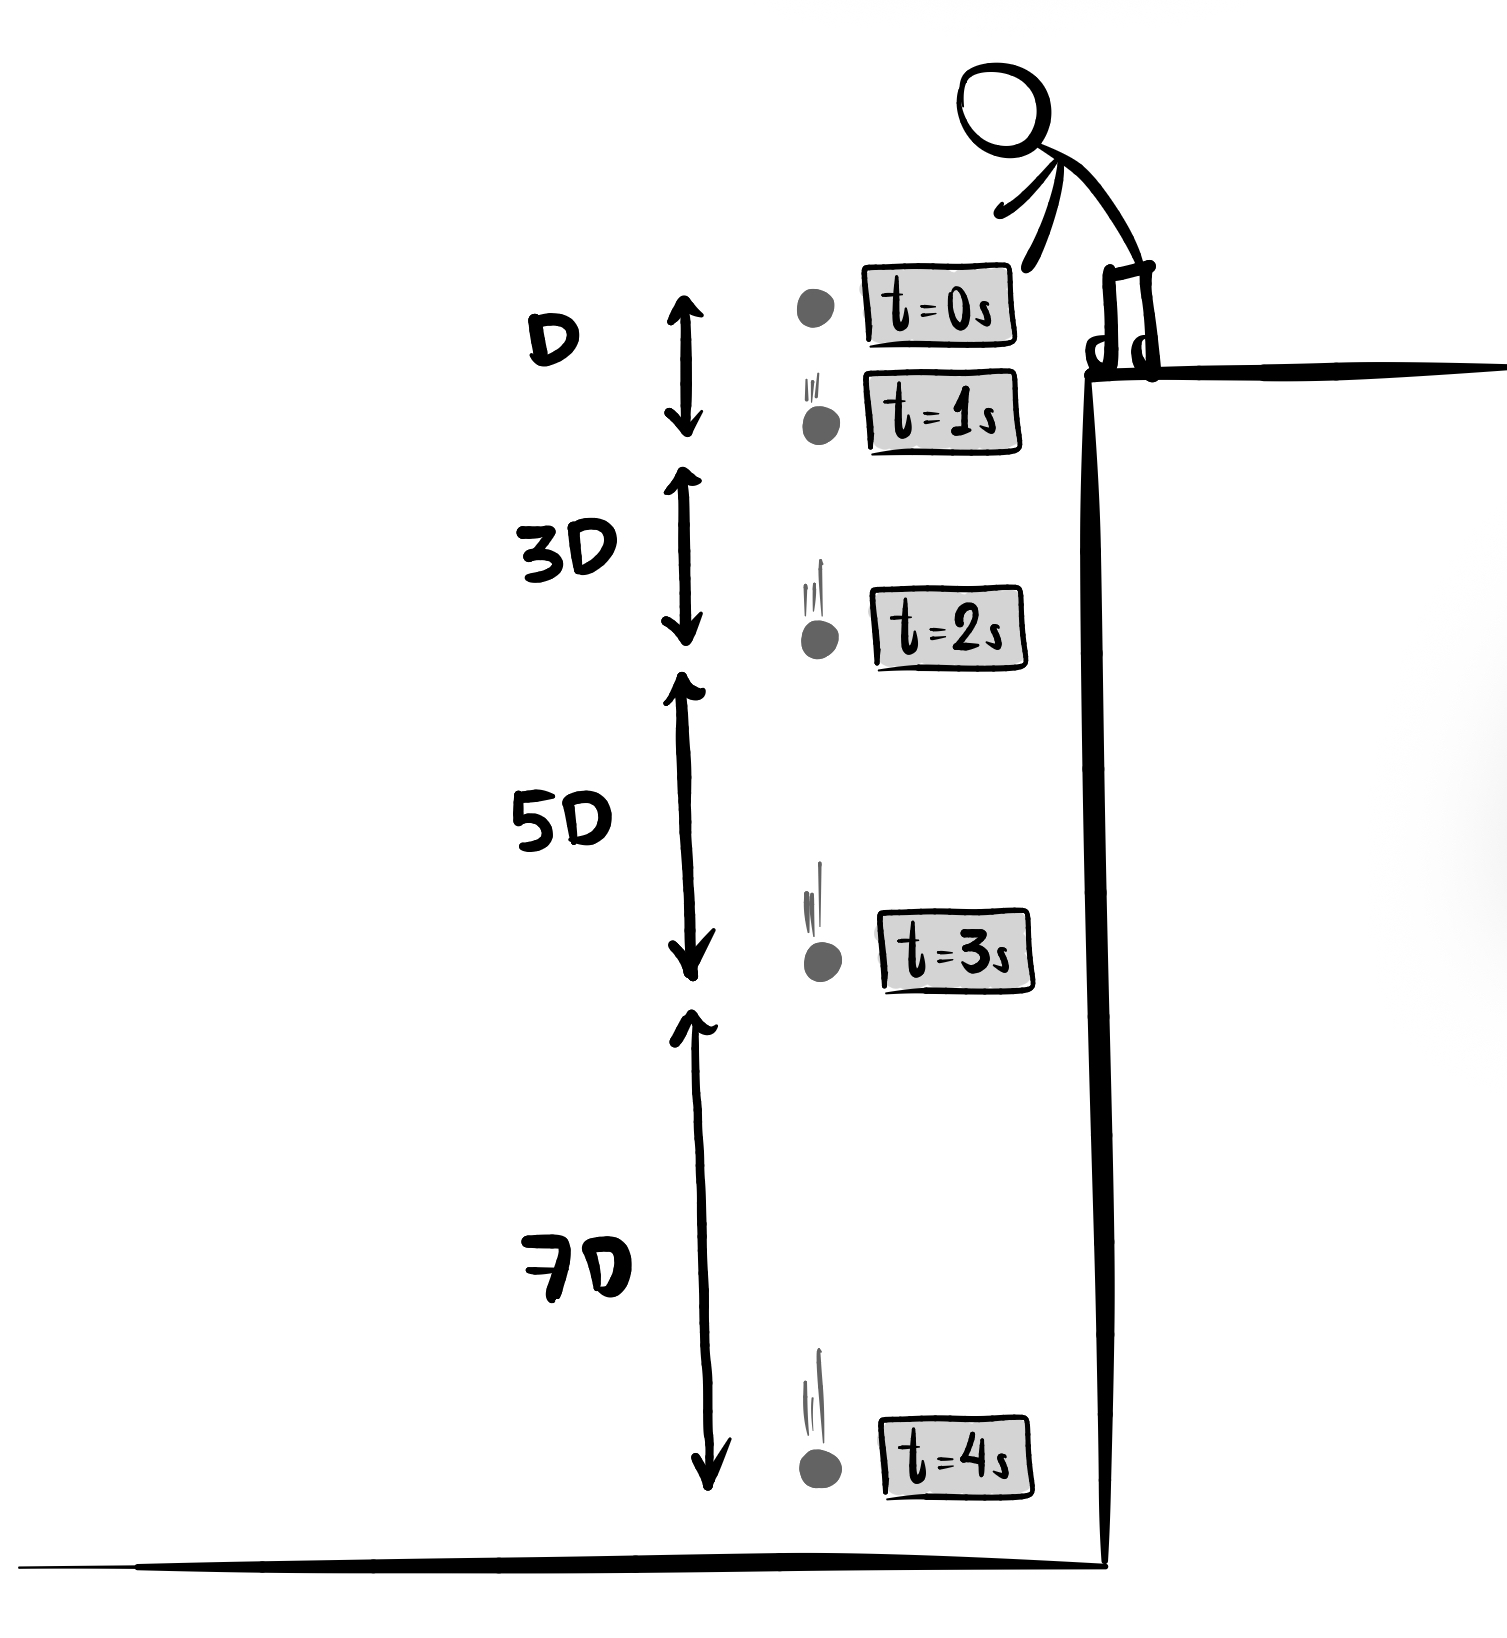
\includegraphics[scale=0.16]{imagensintro/quedalivre.jpeg}};
      \end{scope}
    \end{tikzpicture}
    \caption{Tentando novamente transmitir informações por meio de um desenho.}
    \label{intro02}
\end{figure}

Uma forma de te transmitir o resultado deste experimento é te entregando um desenho como o da Figura \ref{intro02}, que tenta sintetizar o que foi feito e qual foi o resultado obtido. Alguém poderia alegar que nem todos poderiam extrair de tal desenho exatamente o que seria necessário, por mais que o autor tenha colocado empenho e dedicação em fazer um bom desenho que fosse o mais fiel possível ao experimento realizado. Uma outra forma, talvez mais objetiva e que evite ambiguidade, seria dizer que

\begin{center}
    \textit{Ao fazer o experimento de abandonar uma pedra do repouso e deixá-la cair\footnote{Sem resistência do ar.}, nota-se que as distâncias percorridas em intervalos de tempo iguais e sucessivos estão na proporção dos números ímpares.}
\end{center}

Talvez isso lhe pareça ainda um pouco confuso --- e certamente poderíamos ter dado um jeito de expressar isso em língua portuguesa de forma mais clara --- mas essa foi exatamente a forma como Galileu Galilei, no século XVII, enunciou a chamada lei da Queda Livre, ao realizar tal experimento.

Um outro modo de sintetizar a mesma informação é dizendo que, sendo $s$ a distância vertical que a pedra percorre a partir do repouso (do ponto em que ela é abandonada) e sendo $t$ o tempo de movimento, contado a partir do instante em que a pedra é abandonada, então

\begin{equation}
    s = kt^2,
    \label{00intro_eq_quedalivre}
\end{equation}
em que $k$ é alguma constante.

Talvez a Equação \eqref{00intro_eq_quedalivre} soe, para o leitor, tão grego quanto a frase em grego anteriormente citada. Se este é o caso, tudo bem: não espero que você, a essa altura, tenha compreendido tudo.\footnote{Para o leitor mais afoito e curioso, note que em $t=1$ teríamos $s=k$; em $t=2$ teríamos $s=4k$; em $t=3$ teríamos $s=9k$; e por aí vai. Para avaliar a distância que a pedra percorre em intervalos \textbf{sucessivos} de tempo, teríamos que pegar a diferença entre suas posições em instantes consecutivos de tempo, isto é, a distância percorrida no segundo entre $t=1$ e $t=2$ seria a diferença entre $4k$ e $k$, ou seja, $3k$. A distância percorrida no segundo entre $t=2$ e $t=3$ seria a diferença entre $9k$ e $4k$, ou seja, $5k.$ Percebeu de onde surgem os números ímpares?} Contudo, é preciso notar que, até aqui, temos, a princípio, três formas de exprimir a informação a respeito do que observamos em nosso experimento:

\begin{itemize}
    \item [(i)] Por meio de um desenho, como o da Figura \ref{intro02}.

    \item [(ii)] Por meio da língua portuguesa (ou do grego, para gregos; ou mandarim, para chineses) em uma frase como

\begin{center}
    \textit{Ao fazer o experimento de abandonar uma pedra do repouso e deixá-la cair, nota-se que as distâncias percorridas em intervalos de tempo iguais e sucessivos estão na proporção dos números ímpares.}
\end{center}

  \item [(iii)] Por meio de uma fórmula matemática, como a Equação \eqref{00intro_eq_quedalivre}.
    
\end{itemize}



A primeira forma certamente possui suas limitações: um desenho é algo um pouco subjetivo e pode dar margem para interpretações equivocadas ou ambiguidades, por melhor e mais detalhado que ele tenha sido feito. Entre as formas $(ii)$ e $(iii)$ de se exprimir a informação, o leitor --- por mais que não compreenda como a equação $s=kt^2$ contém a informação de que as distâncias percorridas em intervalos de tempos iguais estão na proporção dos números ímpares --- há de concordar que o caminho $(iii)$ é superior: ele é o mais sucinto de todos. Por mais que a este momento lhe pareça grego, se você acreditar que a Equação \eqref{00intro_eq_quedalivre} contém toda a informação a respeito do resultado do experimento, você terá que concordar que, expressar tudo isso usando apenas 3 letras, 1 número e 1 caractere especial (o símbolo de igualdade) como tal equação faz é algo extremamente sofisticado. E melhor: não precisa de tradução. Pelo caminho $(ii)$ nós teríamos que traduzir para o grego, para o mandarim ou para algum outro idioma caso a conversa fosse com um estrangeiro. Já o caminho $(iii)$ não: ele é uma linguagem universal. Desde que se entenda tal linguagem --- a matemática --- um grego, um brasileiro, um chinês ou um russo seriam capazes de compreender e extrair a informação a respeito de como a natureza funciona ao soltarmos uma pedra do alto de um prédio.

Com isso, o leitor deve ter compreendido agora o que é uma fórmula de física: é uma forma de se expressar, por meio da linguagem matemática, uma informação.\footnote{É por isso que alocar energia para memorizar uma fórmula, sem compreender qual é a informação que ela se propõe a sintetizar, é uma grande perda de tempo. O foco deve estar sempre em compreender a informação e, posteriormente, entender como e por que tal fórmula matemática a sintetiza. É o que faremos nessa jornada.} Tal informação pode ser o resultado de um experimento, por exemplo, e ela poderia muito bem ser expressa por meio da língua falada, de um desenho ou de algum outro método qualquer --- todas essas outras formas são, contudo, bem menos eficientes, como já argumentamos.

Acontece que o terceiro caminho --- expressar o resultado de como a natureza se comporta por meio de uma fórmula matemática --- é superior a todos os demais por um outro fato: a natureza revela os seus padrões por meio da matemática. Por que isso ocorre, ninguém sabe muito bem \footnote{Inclusive, um grande físico, Eugene Wigner, vencedor do prêmio Nobel de Física de 1963, escreveu um artigo famoso intitulado \textit{The Unreasonable Effectiveness of Mathematics in the Natural Sciences} , em que ele concluiu que o fato de a matemática funcionar de modo extremamente eficaz para explicar a natureza é algo inexplicável, quase um milagre.} Mas o fato é que isso ocorre, e foi percebido pela primeira vez possivelmente por Galileu, que escreveu que

\begin{quote}
    A filosofia (isto é, a ciência) está escrita neste grandíssimo livro que, continuamente, está aberto diante de nossos olhos (eu quero dizer o universo), mas que não se pode entender se não se aprende a entender a língua, e a conhecer os caracteres, nos quais está escrito. Ele é escrito em língua matemática, e os caracteres são os triângulos, círculos, e outras figuras geométricas, sem cujos meios é humanamente impossível entender uma só palavra; sem esses é um vão caminhar por um obscuro labirinto.
\end{quote}


Ora, se a natureza não fala por palavras, mas sim por relações matemáticas, as equações são o modo mais honesto e eficiente que encontramos para escutá-la, estudá-la e compreendê-la. Para concluir essa introdução, espero que até aqui tenha ficado claro para o leitor: \textbf{uma fórmula de física é simplesmente um meio de se expressar, matematicamente, uma informação a respeito da natureza. Tal forma é a mais eficiente e objetiva, uma vez que a natureza se expressa em linguagem matemática.} Cabe destacar que, por meio da linguagem matemática, torna-se possível mensurar e transmitir informações quantitativas de forma mais precisa. Por exemplo, no contexto da Figura \ref{intro01}, é possível, por meio de uma equação matemática, expressar --- por meio de grandezas físicas adequadas --- o quão quente estava aquele dia ou o quão brilhante estava o sol, informações estas que seriam difíceis de se transmitir com precisão em palavras. Agora que o leitor já tem essa clareza, vamos aos 3 tipos de fórmulas que podemos encontrar.




\section{Os 3 tipos de equações físicas}

Note que o título dessa seção carrega o termo \textit{equações físicas} e não mais \textit{fórmulas de física}. No final do dia estou falando da mesma coisa, mas, dada a introdução feita, já está claro para o leitor que não há nada de mágico na Física e em suas equações matemáticas. Contudo, acredito que o termo ``fórmula'' acaba carregando essa conotação de algo meio místico, que ocorre como em uma fórmula mágica, em que se coloca as variáveis e ela, misticamente, lhe cospe o resultado, sem que ninguém entenda como isso é feito. Como estamos construindo um entendimento que vai na contramão disso, daqui em diante, sempre que me referir a uma fórmula matemática qualquer de física, vou usar o termo \textbf{equação}, para deixar, desde já, essa noção equivocada e ultrapassada do lado de fora --- seja do nosso entendimento ou mesmo do nosso vocabulário.


Dito isso, todas as centenas de fórmulas de física que você puder ver por aí serão, certamente, de um tipo específico entre três possíveis. Compreender esses três grupos de equações e entender suas diferenças certamente ajudará você a entender melhor as fórmulas, o que são e quando devem ser usadas.



\subsection{Definições} \label{subsecao_introducao_eqsdefinicoes}

O primeiro tipo de equação, as \textbf{definições}, são aquelas que são definidas, ou seja, criadas. Isso mesmo, elas são inventadas pelos físicos. Para você que desconfiava que esse negócio de fórmulas de física era tudo tirado da cabeça de algum maluco: você esteve certo o tempo inteiro. Pelo menos para esse primeiro tipo de fórmula, e você vai entender o motivo.

Digamos que você está na mesa, com sua família, tomando café. De repente você se vê na necessidade de pedir para o seu companheiro lhe passar o item da Figura \ref{intro03}. Porém, considere que a palavra \sout{colher} não existe, ou seja, o item em questão é conhecido por todos, mas não possui um nome atribuído a ele. 


\begin{figure}[h]
    \centering
    \begin{tikzpicture}
      \begin{scope}[blend mode=multiply]
        \node {
\includegraphics[scale=0.18]{imagensintro/colher.png}};
      \end{scope}
    \end{tikzpicture}
    \caption{O objeto que todos conhecem mas que não possui um nome.}
    \label{intro03}
\end{figure}

Você primeiro tenta apontar para o objeto, pedindo que lhe entreguem. Porém tal objeto está misturado com algumas facas, garfos e outros itens de cozinha, de modo que o interlocutor acaba confundindo a direção para qual você aponta e lhe entrega uma faca. Em seguida, observando que apontar pode não ser a melhor forma para estabelecer a comunicação de forma precisa, você tenta descrever o objeto do qual precisa, e diz algo como \textit{``me dê aquele objeto usado para pegar o açúcar''}, quando o interlocutor, meio na dúvida do que você quer, lhe passa um pote de açúcar. Tomado pela frustração, você decide levantar da cadeira e ir pegar a colher sem fazer uso de intermediários.

Esse diálogo fictício e simples serve para apontar uma coisa: a importância do estabelecimento da linguagem para que haja comunicação. Toda essa confusão e ambiguidade se eliminaria caso nós simplesmente acordássemos em chamar, daqui em diante, tal objeto sem nome de \textit{colher}: pronto, eis o acordo! Agora a comunicação é possível. 

Note que, aparentemente, fizemos algo absurdo: --- pelo menos é assim que você deve pensar no caso das fórmulas de física --- tivemos que inventar um nome!\footnote{Imagine só que absurdo, inventar uma fórmula...} Eu não sei bem qual é a etimologia da palavra colher, mas vamos imaginar que, um dia, um certo antepassado nosso, digamos, de nome Jairo, tomado pela mesma frustração que você ao não conseguir identificar tal objeto, decide inventar um nome e resolver essa palhaçada: eis que no dia 13 de abril do século III a.C. Jairo batiza tal objeto, levantando da mesa, em postura ereta, peito estufado, ele pega o objeto na mão direita, erguendo-o para o alto, com o braço esticado. Com uma xícara de café na mão esquerda, sobe na cadeira e grita a proclamação para os seus familiares:

\begin{center}
  \textit{``Doravante, tal objeto deve ser referenciado pelo nome \textit{colher!''}}.    
\end{center}

Todos se emocionam e batem palmas. Alguns choram de emoção, outros, tomados por tamanha emoção, ficam imóveis, mas com o semblante transmitindo êxtase. Que dia, meus amigos...! Quisera eu estar ali para presenciar este inédito feito na história da humanidade, que extinguiu, de uma vez por todas, os problemas de comunicação nas mesas de café da manhã de todas as famílias do mundo.

Note a importância do acordo --- termos combinado que o nome daquele objeto é colher --- para que possa haver uma comunicação clara e precisa. O poema \textit{Revelação}, de Viviane Mosé, evidencia isso:\footnote{Os trechos em negrito são destaques feitos pelo autor}


\begin{quote}
    Eu queria dizer uma coisa que eu não posso sair dizendo por aí.\\
É um segredo que eu guardo, é uma revelação\\
Que eu não posso sair dizendo por aí.\\
É que eu tenho medo de que as pessoas se desequilibrem delas mesmas.\\
Que elas caiam quando eu disser.\\
É que eu descobri que a palavra não sabe o que diz.\\
A palavra delira. A palavra diz qualquer coisa.\\
A verdade é que a palavra, ela mesma, em si própria, não diz nada.\\
\textbf{Quem diz é o acordo estabelecido entre quem fala e quem ouve.}\\
\textbf{Quando existe acordo existe comunicação,}\\
Mas quando esse acordo se quebra ninguém diz mais nada,\\
Mesmo usando as mesmas palavras.
\end{quote}



Nessa analogia o nome que demos a um objeto seria a nossa ``fórmula'' (ou melhor, a grandeza física definida por essa fórmula). Ora, poderíamos ter enfrentado um problema semelhante à impossibilidade do diálogo a respeito da colher em uma situação diferente. Digamos que vivemos em uma época na história da humanidade em que o conceito de \sout{velocidade} não existe. Eu quero tentar lhe transmitir a situação que ocorre na Figura \ref{intro04}, que retrata o movimento de um carro e de um ônibus.




\begin{figure}[h]
    \centering
    \begin{tikzpicture}
      \begin{scope}[blend mode=multiply]
        \node {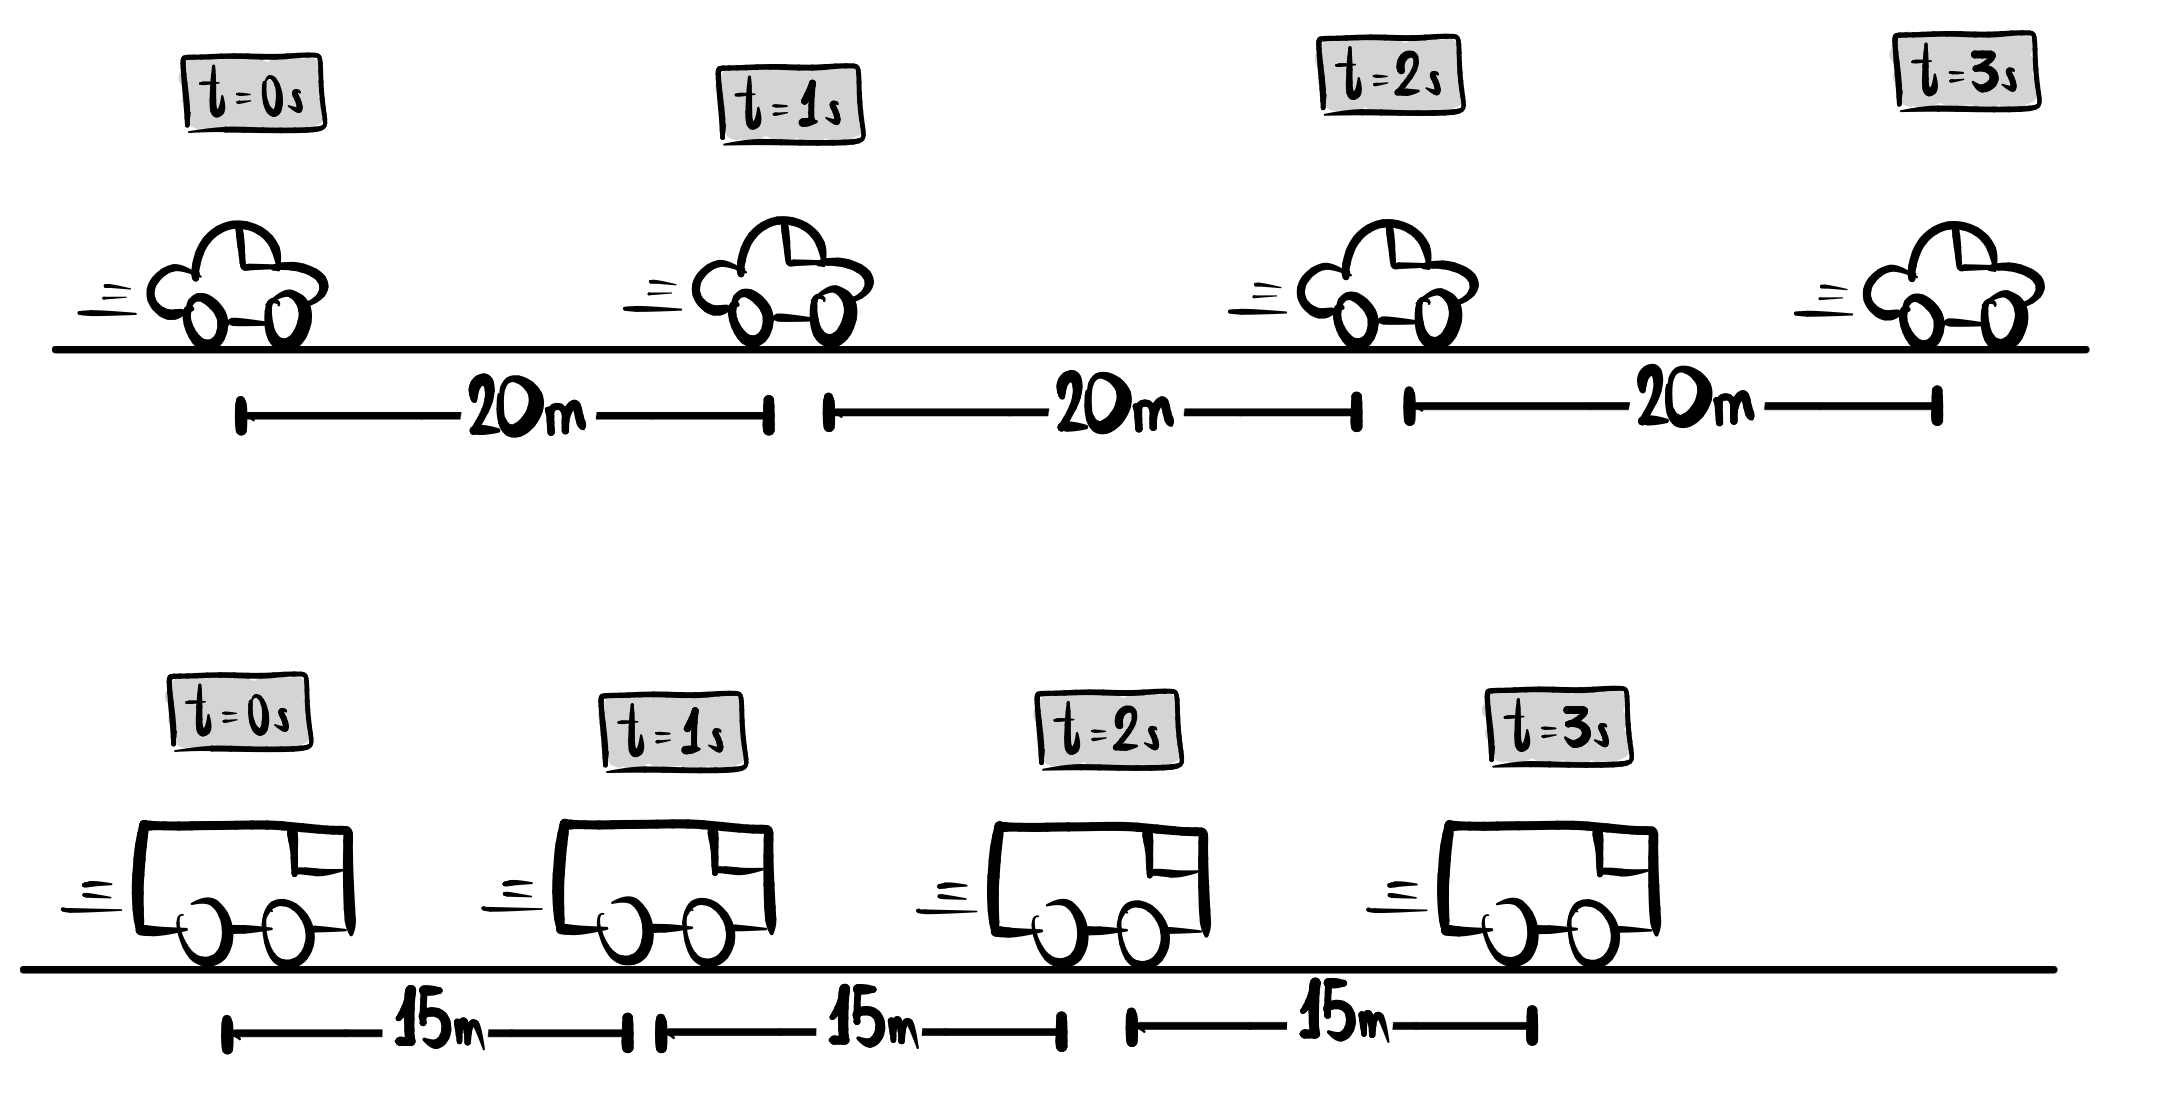
\includegraphics[scale=0.18]{imagensintro/carros.jpeg}};
      \end{scope}
    \end{tikzpicture}
    \caption{Comparando o movimento de dois objetos em um universo em que o conceito de velocidade é inexistente.}
    \label{intro04}
\end{figure}


Eu poderia começar lhe dizendo que existe um carro e um ônibus, os dois se movendo em uma mesma direção, porém o carro anda mais depressa que o ônibus. Isso estaria correto, porém um pouco incompleto. O quão mais depressa se move esse carro? 
% Poderíamos tentar observar qual dos dois teria mais \emph{tracinhos} atrás, mas isso dependerá do cuidado e esmero de quem fez as imagens para transmitir a rapidez de cada um com precisão.

Note que, para tentar dizer isso, eu começaria, em alguma medida, a enfrentar problemas parecidos com aquele da mesa do café da manhã, pela simples razão de limitação linguística --- não há um termo para medir o quão rápido algo se move na nossa linguagem, pelo menos até então. 

Eu poderia, então, lhe dizer que o carro anda cinco metros a mais que o ônibus em um mesmo intervalo de tempo, o que estaria correto, mas ainda deixaria espaço para imprecisão: você poderia pensar que o ônibus anda, a cada segundo, 80 metros, enquanto o carro andaria 85 metros. Quaisquer combinações de números em que um deles é cinco unidades maior do que o outro funcionariam e a informação que eu lhe transmiti, portanto, deixaria um grande espaço para ambiguidade. 

Talvez eu pudesse então logo lhe dizer o seguinte: \textit{existe um ônibus e um carro se movendo, em uma mesma direção e sentido, e enquanto o ônibus avança 15 metros, o carro avança 20 metros.} Pronto, agora não há espaço algum para ambiguidade: qualquer um conseguiria reconstruir, do zero, a Figura \ref{intro04} com base nessa informação. Quer dizer...alguém poderia, com base nessa informação, desenhar uma figura em que o carro avança 20 metros em 1 hora e o ônibus avança 15 metros durante essa mesma hora. Isso estaria coerente com a informação que fora transmitida, porém incoerente com a situação física real. 

Cansado de tentar explicar de forma sucinta a situação em questão, você simplesmente abandona tal missão e resolve descrever, \textit{ipsis litteris}, o que vê na figura: \textit{existe um ônibus e um carro se movendo na mesma direção e sentido, e enquanto o ônibus avança 15 metros durante o intervalo de tempo de 1 segundo, o carro avança 20 metros, neste mesmo intervalo de tempo de 1 segundo.}

Pronto, deu-se cabo de tal tarefa: não haverá cristão que discorde que tal frase transmite, na íntegra, toda a situação física da Figura \ref{intro04}. O que é verdade, porém foram necessárias algumas tentativas e, por fim, uma frase de três linhas para dar conta de tal tarefa.

Digamos, portanto, que, tal como nosso amigo Jairo o fez com a colher, resolvamos criar um novo conceito --- uma nova palavra --- para possibilitar facilitar e comunicar situações como as da Figura \ref{intro04}. Incumbido de tal missão, eis que o leitor, inspirado pelo espírito e feito de Jairo, sobe na cadeira, com o peito estufado, braço direito erguido e postura ereta, e grita aos que estão à sua volta:

\begin{center}
    \textit{Doravante, a razão entre a distância percorrida por um corpo e o intervalo de tempo no qual tal distância é percorrida será chamada de velocidade!}
\end{center}

Pronto: foi feito o batismo. Todos se emocionam e se arrepiam diante da grande honra que é viver tal momento em que uma nova grandeza física é criada. Em termos matemáticos, o que você fez foi dizer que, sendo $d$ a distância que um objeto percorre em um intervalo de tempo $\Delta t$, a sua velocidade, a qual denominaremos por $v$, é dada por

\begin{equation}
   \boxed{ v := \dfrac{d}{\Delta t}.}
   \label{00intro_eq_velocidade}
\end{equation}

E sim, é isso mesmo. Tal como foi necessário para Jairo criar um nome para um objeto a fim de ampliar sua capacidade de comunicação, o mesmo foi feito por nós: criamos um nome e uma equação matemática que \textbf{define} uma nova grandeza física, com o simples intuito de possibilitar que o estudo e a análise de situações como as da Figura \ref{intro04} sejam simplificados. 

Agora, analisando tal imagem e incumbido da nobre missão de transmitir toda a sua informação a alguém que não a viu, você poderia simplesmente dizer que:

\textit{Existe um ônibus e um carro se movendo, em uma mesma direção e sentido, sendo suas velocidades de $15$ m/s e $20$ m/s, respectivamente.}

Desde que esteja acordado e convencionado entre nós o que se trata o termo \textit{velocidade} --- tal e qual precisa estar acordado a que se refere o termo \textit{colher} --- tal frase transmite, com simplicidade, toda a informação física do contexto.



Algumas observações merecem ser feitas a respeito de tal definição:

\begin{itemize}
    \item [(i)] Simbologia

    O símbolo $:=$ que usamos talvez seja novo para o leitor. Confesso que acho seu uso desnecessário para o estudante de primeira viagem, mas fiz questão de usá-lo para deixar clara a natureza da equação física que apresentamos. Tal símbolo significa justamente que está ocorrendo uma definição, e é comum de ser utilizado assim que definimos (batizamos ou criamos, caso o leitor assim prefira) uma grandeza pela primeira vez. A fim de deixar nítida a diferença para o sinal de igualdade, perceba que as equações devem ser lidas como:

    \begin{align}
        v &= \sfrac{d}{\Delta t} \rightarrow v \text{ é igual a } d \text{ dividido por } \Delta t .\nonumber \\ 
        v &:= \sfrac{d}{\Delta t} \rightarrow v \text{ é definido como sendo } d \text{ dividido por } \Delta t  .\nonumber
    \end{align}

Uma vez que \textbf{definimos} $v$ como sendo $d$ dividido por $\Delta t$, é claro que $v$ passa ser \textbf{igual} a $d$ dividido por $\Delta t$, por definição. 

Ou seja, após o termo ter sido definido, podemos tranquilamente usar o símbolo de igualdade daí em diante, já que uma coisa equivale a outra. O símbolo $:=$, portanto, será usado exclusivamente na primeira vez em que estivermos definindo uma grandeza, e ele já deixará clara a natureza da equação física em questão: não se trata de uma equação experimental ou demonstrável, mas sim de uma definição.

    \item [(ii)] Significado

    De fato, o que estamos fazendo é realmente criar um novo termo: uma nova grandeza física. Isso não deveria lhe soar estranho, ou pelo menos não mais estranho do que o fato de que um dia alguém batizou o objeto da Figura \ref{intro01} como colher e começamos a nos referir a tal utensílio por tal nome, desde então. 
    
    Inventar verbos, criar nome para objetos ou para grandezas físicas faz parte da construção da linguagem, o que nos permite ampliar nossa capacidade, precisão e especificidade da comunicação. Seria muito difícil você expressar, em palavras, que gosta muito de alguém em uma sociedade na qual as palavras \textit{gostar} e \textit{amar} não existissem; da mesma forma que é difícil pedir a alguém uma colher se tal palavra não existe e também é um pouco complicado comparar a rapidez com que objetos se movem caso não exista o conceito de velocidade.
    
    É claro que alguém poderia, a seu bel prazer, criar uma nova grandeza física qualquer. Digamos que tal grandeza seja o número de janelas de uma casa dividido pelo número de portas, tudo isso elevado ao quadrado. Damos o nome a essa grandeza de Rudolph, representado pela letra $r$, e definido, portanto, por:

    $$ r : = \left( \dfrac{\text{número de janelas}}{\text{número de portas}} \right)^2.$$

    Ora, isso pode ser feito, mas qual seria a finalidade de inventarmos tal grandeza? Podemos, em teoria, inventar qualquer palavra ou qualquer grandeza física, mas, se isso não tiver uma finalidade ou serventia clara, certamente não será levado adiante. Acontece que criar uma grandeza física chamada \textit{velocidade} e defini-la conforme a Equação \eqref{00intro_eq_velocidade} parece fazer bastante sentido, uma vez que melhora nossa precisão na comunicação a respeito do movimento dos corpos, como vimos. 
    
    Note que o autor investiu um certo tempo, antes de apresentar tal fórmula, criando um contexto em que, ao final, ficasse claro como que a invenção de tal conceito resolveria alguns problemas de comunicação, eliminaria ambiguidades e possibilitaria que fosse possível transmitir informações a respeito de movimento de corpos com muito mais fluidez. Dito isso, parece fazer sentido criar tal conceito, tal como parecia fazer sentido criar um nome para o talher da Figura \ref{intro03}, fosse ele colher ou qualquer outro. Perceba que o nome da grandeza $v$ ser velocidade é pouco relevante --- caso ela se chamasse qualquer outra coisa ou fosse representada por qualquer outra letra, não teria muito problema. O que é relevante, de fato, é a sua definição matemática: ela representa a razão entre a distância percorrida e o tempo, e é isso, essencialmente, que a define. Do mesmo modo, se o nome do talher da Figura \ref{intro03} fosse, digamos, velocidade, não teria problema: temos um nome associado ao objeto, e isso é tudo que precisamos para estabelecer a comunicação.

    Note que, na grandeza Rudolph, nada disso se aplica: não parece ter sentido, serventia ou utilidade alguma em criar tal grandeza. Ela não facilita a comunicação de nada, até porque o número de janelas de uma casa pode ser importante, o número de portas também, mas ninguém está interessado em saber quanto vale a razão entre essas coisas elevado ao quadrado.

    Dito isso, ao definir qualquer grandeza, é importante que o leitor sempre se atente ao motivo pelo qual aquilo está sendo feito. Há algum sentido e razão em se criar um novo conceito, e é importante compreendê-lo para que o leitor entenda com profundidade o significado de tal equação, tal como fizemos, em parte, para criar o conceito de velocidade.

    

    

    \item [(iii)] Operacional

    Com tudo que construímos até aqui, parece que a única vantagem em se criar uma nova grandeza física, como a velocidade, é linguística: temos agora uma nova palavra, ou melhor, um novo conceito, para poder expressar algo que vemos no mundo. Isso é, em essência, o que Jairo fez ao criar a palavra colher.

    Contudo, esse não é o principal motivo de fazermos isso na Física. A definição de novas grandezas tem um caráter, acima de tudo, operacional. Como veremos, ao desdobrar os estudos da Física, em diversos contextos a rapidez com que um corpo se move ao longo do tempo --- a velocidade --- é um conceito que irá aparecer repetidas vezes, de modo que uma série de equações assumirão um caráter mais simples em termos dessa grandeza. Enuncio algumas delas abaixo, apenas para que o leitor tenha um gosto a respeito da importância de se criar o conceito de velocidade $v$:

    %$$ E_c = \dfrac{1}{2}mv^2 \text{  ;  } a_c = \dfrac{v^2}{R} \text{  ;  } F_M = Bqv \sin \theta \text{  ;  } \gamma = \dfrac{1}{\sqrt{1-\sfrac{v^2}{c^2}}}.$$

\[
\underbrace{E_c = \frac{1}{2}mv^2}_{\text{Energia cinética}} \quad ; \quad
\underbrace{a_c = \frac{v^2}{R}}_{\text{Aceleração centrípeta}} \quad ; \quad 
\underbrace{F_M = Bqv\sin\theta}_{\text{Força magnética}} \quad ; \quad
\underbrace{\gamma = \frac{1}{\sqrt{1 - \frac{v^2}{c^2}}}}_{\text{Fator de Lorentz}}
\]


Todas essas equações expressam grandezas físicas em termos de outras grandezas, sendo uma delas a velocidade $v$. Desse modo, ter criado o conceito de velocidade definido da forma como foi feito na Equação \eqref{00intro_eq_velocidade} se mostrará algo extremamente relevante: construiremos outras grandezas, equações e teorias em cima de tal noção, o que nos trará uma vantagem operacional ao longo dos cálculos.

\end{itemize}



Por fim, que fique claro para o leitor: as equações desse tipo --- as definições --- são expressões matemáticas que não descrevem a natureza, mas sim criam o vocabulário com o qual a natureza será descrita. O que estamos fazendo aqui, como a poetisa escreveu nos versos, é estabelecer o acordo para que consigamos fazer uma boa comunicação. Este é o primeiro tipo de equação que o leitor precisa conhecer. Note que, ao definirmos o conceito de velocidade, não estamos dizendo absolutamente nada a respeito de como a natureza funciona. Estamos apenas estabelecendo a linguagem que iremos utilizar para, aí sim, estudar a natureza e entender como ela funciona. \footnote{Como o objetivo desse tipo de equação é criar o vocabulário para construir, em cima dele, o conhecimento teórico, o leitor há de notar que, ao iniciar o estudo de uma nova parte da Física, quase sempre ele começará por meio de algumas definições. Ao começar o estudo de movimento precisamos criar o conceito de velocidade, de aceleração...ao começar o estudo de circuitos elétricos precisamos criar o conceito de corrente elétrica --- isto é, definir esta nova grandeza em termos de outras --- ao começar o estudo de óptica precisaremos definir o que é o índice de refração, e por aí vai. }




\subsection{Equações Experimentais}

O segundo tipo de equação que podemos encontrar na Física é o das equações experimentais. Esse tipo de equação não é uma invenção humana, logo, sua razão de ser não é estabelecer o vocabulário que será usado para o estudo. Equações desse tipo expressam, em linguagem matemática, como a natureza se comporta em certo contexto ou fenômeno. Ou seja, faz-se um experimento, digamos, como o da Figura \ref{intro02}, e sintetiza-se, matematicamente, o resultado de tal experimento por meio de um equação, como a Equação \eqref{00intro_eq_quedalivre}. Perceba que nós não inventamos tal equação\footnote{Pode haver alguma ambiguidade entre equações experimentais e equações demonstráveis, que serão as próximas a serem estudadas. Sobre isso, sugerimos ao leitor, após concluir a introdução e avançar bastante ao longo do texto para ganhar um pouco mais de maturidade, ler o \autoref{apendice-eqs-exp-vs-dem}.} --- e ela tampouco se propõe a definir ou criar algum conceito. Ela simplesmente traduz, em linguagem matemática, o que foi observado no experimento.

Para citar um outro exemplo, observe a Figura \ref{intro07}, que mostra duas cargas elétricas positivas, de cargas $Q_1$ e $Q_2$, separadas por uma distância $r$.

\begin{figure}[h]
    \centering
    \begin{tikzpicture}
      \begin{scope}[blend mode=multiply]
        \node {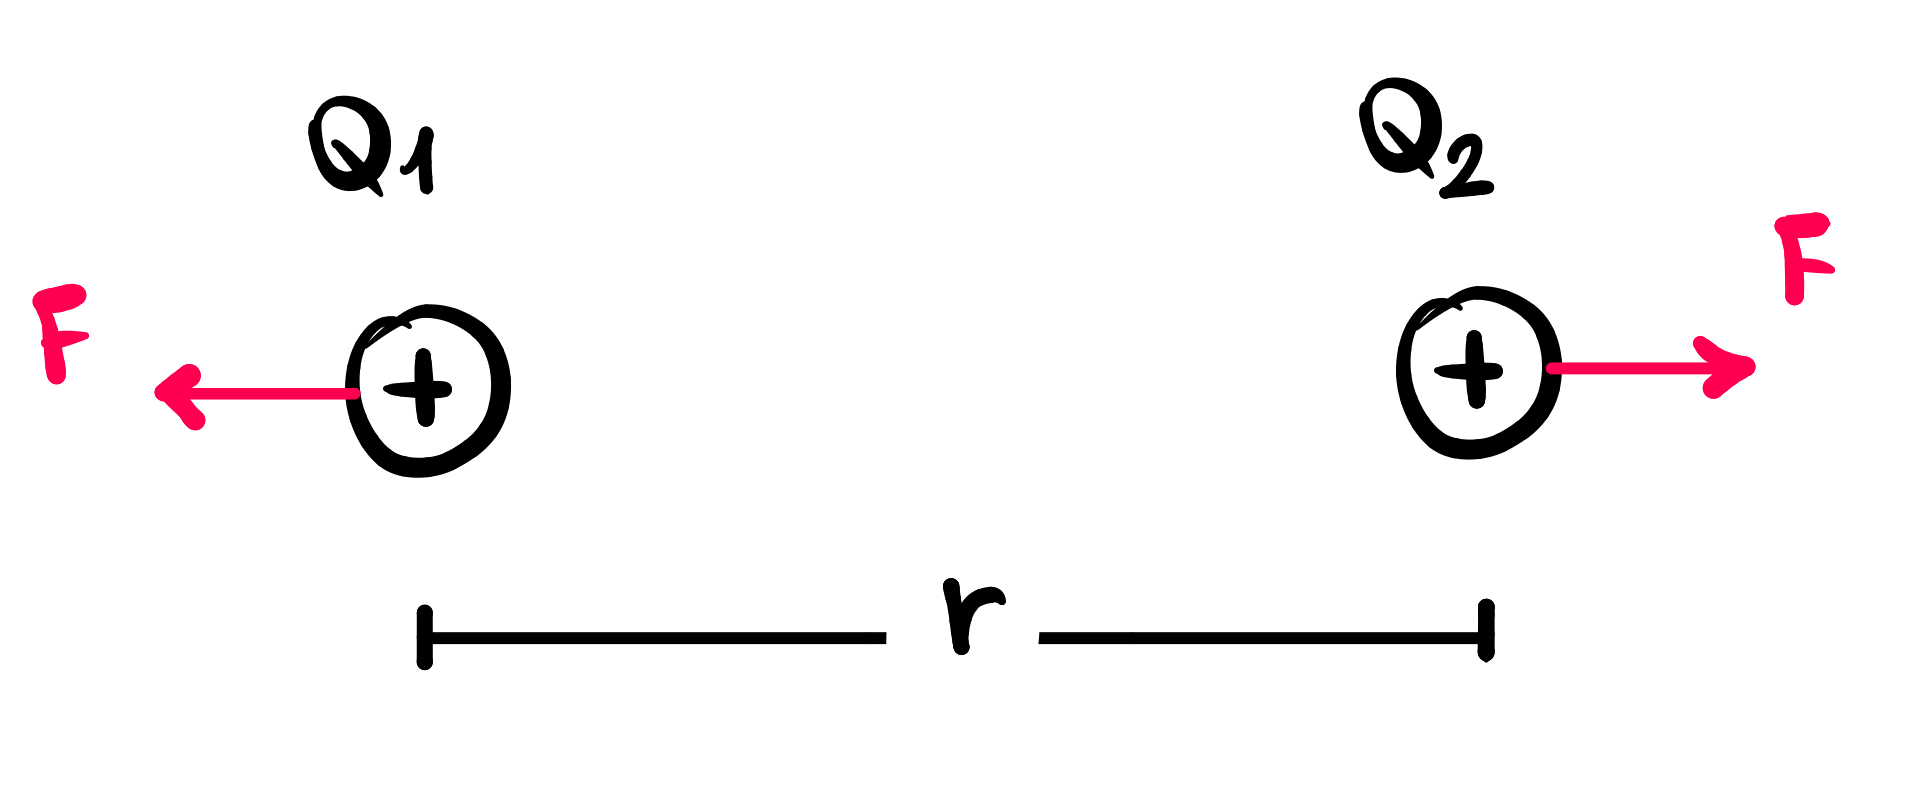
\includegraphics[scale=0.12]{imagensintro/coulomb.jpeg}};
      \end{scope}
    \end{tikzpicture}
    \caption{A força eletrostática entre duas cargas elétricas $Q_1$ e $Q_2$.}
    \label{intro07}
\end{figure}


Já era conhecido, desde o século XVII, que corpos eletrizados poderiam se atrair ou se repelir, porém ninguém sabia exatamente como poderíamos computar tal força. Em 1785, um físico francês chamado Charles-Augustin de Coulomb introduziu um aparato, chamado balança de torção, que o possibilitou fazer alguns experimentos para identificar como se dava tal força (explicaremos em mais detalhes o que é isso e como o experimento foi feito no momento adequado).

Ao fazer vários experimentos, com diferentes valores de cargas elétricas $Q$ e diferentes valores de distância $r$ entre as cargas, o aparato de Coulomb possibilitava medir a força elétrica entre as cargas da Figura \ref{intro07}. Após várias medições, foram percebidos dois fatos experimentais fundamentais:

\begin{itemize}
    \item A força é proporcional ao produto das cargas $Q_1 \cdot Q_2.$
    \item A força diminui com o quadrado da distância entre as cargas, ou seja, é proporcional a $\dfrac{1}{r^2}.$
\end{itemize}


Nada disso foi definido ou deduzido. Tudo isso foi inferido a partir de dados experimentais. Com o tempo, foi possível construir uma equação matemática que sintetizasse os dados do experimento, que é a equação conhecida como Lei de Coulomb, dada por

\begin{equation}
    F = k \dfrac{Q_1Q_2}{r^2},
    \label{00intro_eq_coulomb}
\end{equation}
em que $k$ é uma constante que é obtida pelos experimentos. Note que a Equação \eqref{00intro_eq_coulomb} sintetiza os dois fatos que foram observados anteriormente: a força é proporcional ao produto das cargas e inversamente proporcional ao quadrado da distância. Trata-se apenas de se transmitir, matematicamente, a informação a respeito de como a natureza funciona, informação esta que foi obtida por meio da realização de um experimento.

Observe que a Lei de Coulomb não é uma definição: ela não define ou explica o que é uma carga elétrica ou o que é uma força. Ao mesmo tempo, tal lei tampouco explica porque a força tem essa forma, ou como essa força é transmitida de uma carga para outra. Ela apenas afirma que é assim que a força se comporta, como foi observado no experimento.

A essa altura o leitor pode se sentir um pouco insatisfeito, talvez por ter enxergado uma aparente limitação nesse tipo de fórmula, o que pode tê-lo levado a questionamentos como

\begin{center}
    \textit{Temos só que aceitar que a fórmula é essa? De onde vem essa força, e por que ela funciona assim?}
\end{center}

Essa sensação é natural, mas é preciso deixar claro desde já: essa limitação não é um defeito da equação experimental. Ela é, na verdade, sua \textbf{característica essencial.}

Uma equação experimental não pretende explicar por que a natureza funciona de determinado modo.
Ela descreve como a natureza se comporta, dentro de um certo contexto observável.
O experimento nos permite medir, comparar, identificar regularidades e, a partir disso, sintetizar esse comportamento em linguagem matemática. É exatamente isso que a equação expressa: um retrato fiel do \textit{como.}

Por que ela funciona exatamente assim é algo que podemos responder com a criação de alguma teoria mais ampla que tente entender o motivo de tal funcionamento, ou, talvez, nunca conseguiremos responder. Em última instância, sempre chegaremos a alguma pergunta que não conseguiremos responder, que talvez se torne mais filosófica do que física.

%Para exemplificar isso, vamos voltar ao experimento de abandonar a pedra e analisar seu movimento, descrito na Figura \ref{intro02}. O experimento nos permite entender como se dá o movimento da pedra: em intervalos de tempos sucessivos as distâncias percorridas estão na proporção dos números ímpares. Isso pode ser transmitido dessa forma, ou em linguagem matemática, como a Equação \eqref{00intro_eq_quedalivre} se propõe a fazer. Note que, até aqui, não sabemos exatamente porque a pedra cai. Sabemos só que ela cai --- e sabemos que esse movimento evolui ao longo tempo de um jeito específico. Alguém poderia até perguntar: \textit{mas por quê a pedra cai?}.

Para tornar isso concreto, voltemos ao experimento simples de abandonar uma pedra e observar seu movimento, ilustrado na Figura~\ref{intro02}. O experimento nos mostra como a pedra se move: em intervalos de tempo sucessivos, as distâncias percorridas seguem a proporção dos números ímpares. Esse padrão pode ser descrito verbalmente ou condensado em linguagem matemática, como faz a Equação~\eqref{00intro_eq_quedalivre}.

Até aqui, tudo o que sabemos é como a pedra cai. Sabemos que ela cai. Sabemos que seu movimento evolui no tempo de uma forma específica e regular. Mas nada disso responde à pergunta: por que a pedra cai? E é importante perceber que o experimento, por si só, não pode responder a essa pergunta. Esse é precisamente o ponto.

A equação experimental não nasce para explicar causas profundas, mas para organizar o comportamento observado. Ela é uma síntese matemática do que pode ser medido, não uma explicação sobre por que as coisas funcionam como funcionam.

%Perceba que tal experimento não nos permite responder essa pergunta --- e essa é grande característica da equação experimental, como eu estava dizendo. Ela traduz uma síntese de \textit{como} a natureza funciona, que é o que o experimento nos permite medir e identificar, e não do \textit{por que} ela funciona dessa forma. 

É claro que alguém pode, posteriormente, propor uma teoria que tente responder a esse “porquê”. Foi exatamente isso que Newton fez ao formular sua teoria da gravitação. Agora, com essa nova estrutura conceitual, somos capazes de dizer: a pedra cai por causa da gravidade. Mas isso apenas desloca a pergunta. \textit{Por que a gravidade existe? Como ela se propaga? } 

O próprio Newton não saberia responder essas duas últimas perguntas. E, como disse, se formos avançando, provavelmente chegaremos em alguma pergunta que será mais filosófica do que física, e seremos obrigados a parar em algum momento. Em algum momento, talvez, teremos que ficar satisfeitos em entender como a natureza funciona, sem saber exatamente o motivo de ser assim.

É isso. Uma equação experimental é uma síntese matemática de \textit{como} a natureza funciona em um certo contexto. É uma equação que nasce do experimento, não da dedução lógica nem da definição conceitual. Ela surge quando medições revelam regularidades, quando padrões numéricos se repetem e é possível encontrar uma relação matemática simples capaz de condensar os dados.








\subsection{Equações Demonstráveis}

Vamos ao terceiro e último tipo possível de equação que podemos encontrar na Física: equações demonstráveis. Elas não são definições --- não servem para criar vocabulário e estabelecer novos conceitos. Ao mesmo tempo, elas também não são meramente uma expressão do resultado de algum experimento físico. O que elas são, então?

Para responder a essa pergunta, carece voltarmos ao século III a.C. para considerar a estruturação da lógica feita por Aristóteles. O filósofo grego criou o silogismo, que é um raciocínio dedutivo que parte de algumas premissas (afirmações iniciais) para chegar a uma \textbf{conclusão lógica.} O exemplo mais simples e conhecido possivelmente é: 

\begin{quote}
    P1: Todo homem é mortal.\\
    P2: Sócrates é homem.\\
    C: Logo, Sócrates é mortal.
\end{quote}


As duas primeiras frases são as nossas \textit{premissas:} afirmações que aceitamos como verdade. A terceira frase é nossa conclusão: uma consequência lógica e inevitável de termos aceitado como verdadeiras as duas premissas iniciais.

Note que é possível que se discorde das premissas. Alguém poderia questionar se todo homem é mesmo mortal, talvez acreditando que a ciência moderna desenvolverá tecnologias que permitam com que se viva para sempre. Também poderia haver um questionamento sobre Sócrates ser mesmo homem. Quem foi este ser? Será que ele existiu de fato? E, se o fez, quem me garante que ele não era um cachorro, mas sim um homem?

Ora, questionamentos como estes são até válidos, mas note que, se assumirmos as premissas como verdadeiras, a conclusão é inevitável, é absolutamente inquestionável: um estatuto estabelecido --- cuja veracidade depende, naturalmente, da veracidade das premissas. Se a conclusão não for compatível com a realidade --- isto é, se averiguarmos que o tal Sócrates não é mortal --- o erro não estaria na conclusão --- esta é logicamente irrefutável --- e sim nas premissas. Provavelmente teríamos errado ao assumir que todo homem é mortal, ou que Sócrates fosse homem...

Talvez o leitor prefira uma linguagem mais visual para compreender tal raciocínio, o que pode ser feito usando a teoria de conjuntos, como mostra a Figura \ref{intro06}. O que estamos dizendo é que existe um conjunto $M$ de todos os seres que são mortais. A primeira premissa diz que o conjunto $H$ de todos os homens faz parte do tal grupo $M,$ dos mortais. A segunda premissa diz que Sócrates faz parte do grupo $H$, dos homens, de onde devemos concluir, logicamente, que Sócrates, portanto, faz parte do grupo $M$ dos mortais, uma vez que ele contém o grupo dos homens.


\begin{figure}[h]
    \centering
    \begin{tikzpicture}
      \begin{scope}[blend mode=multiply]
        \node {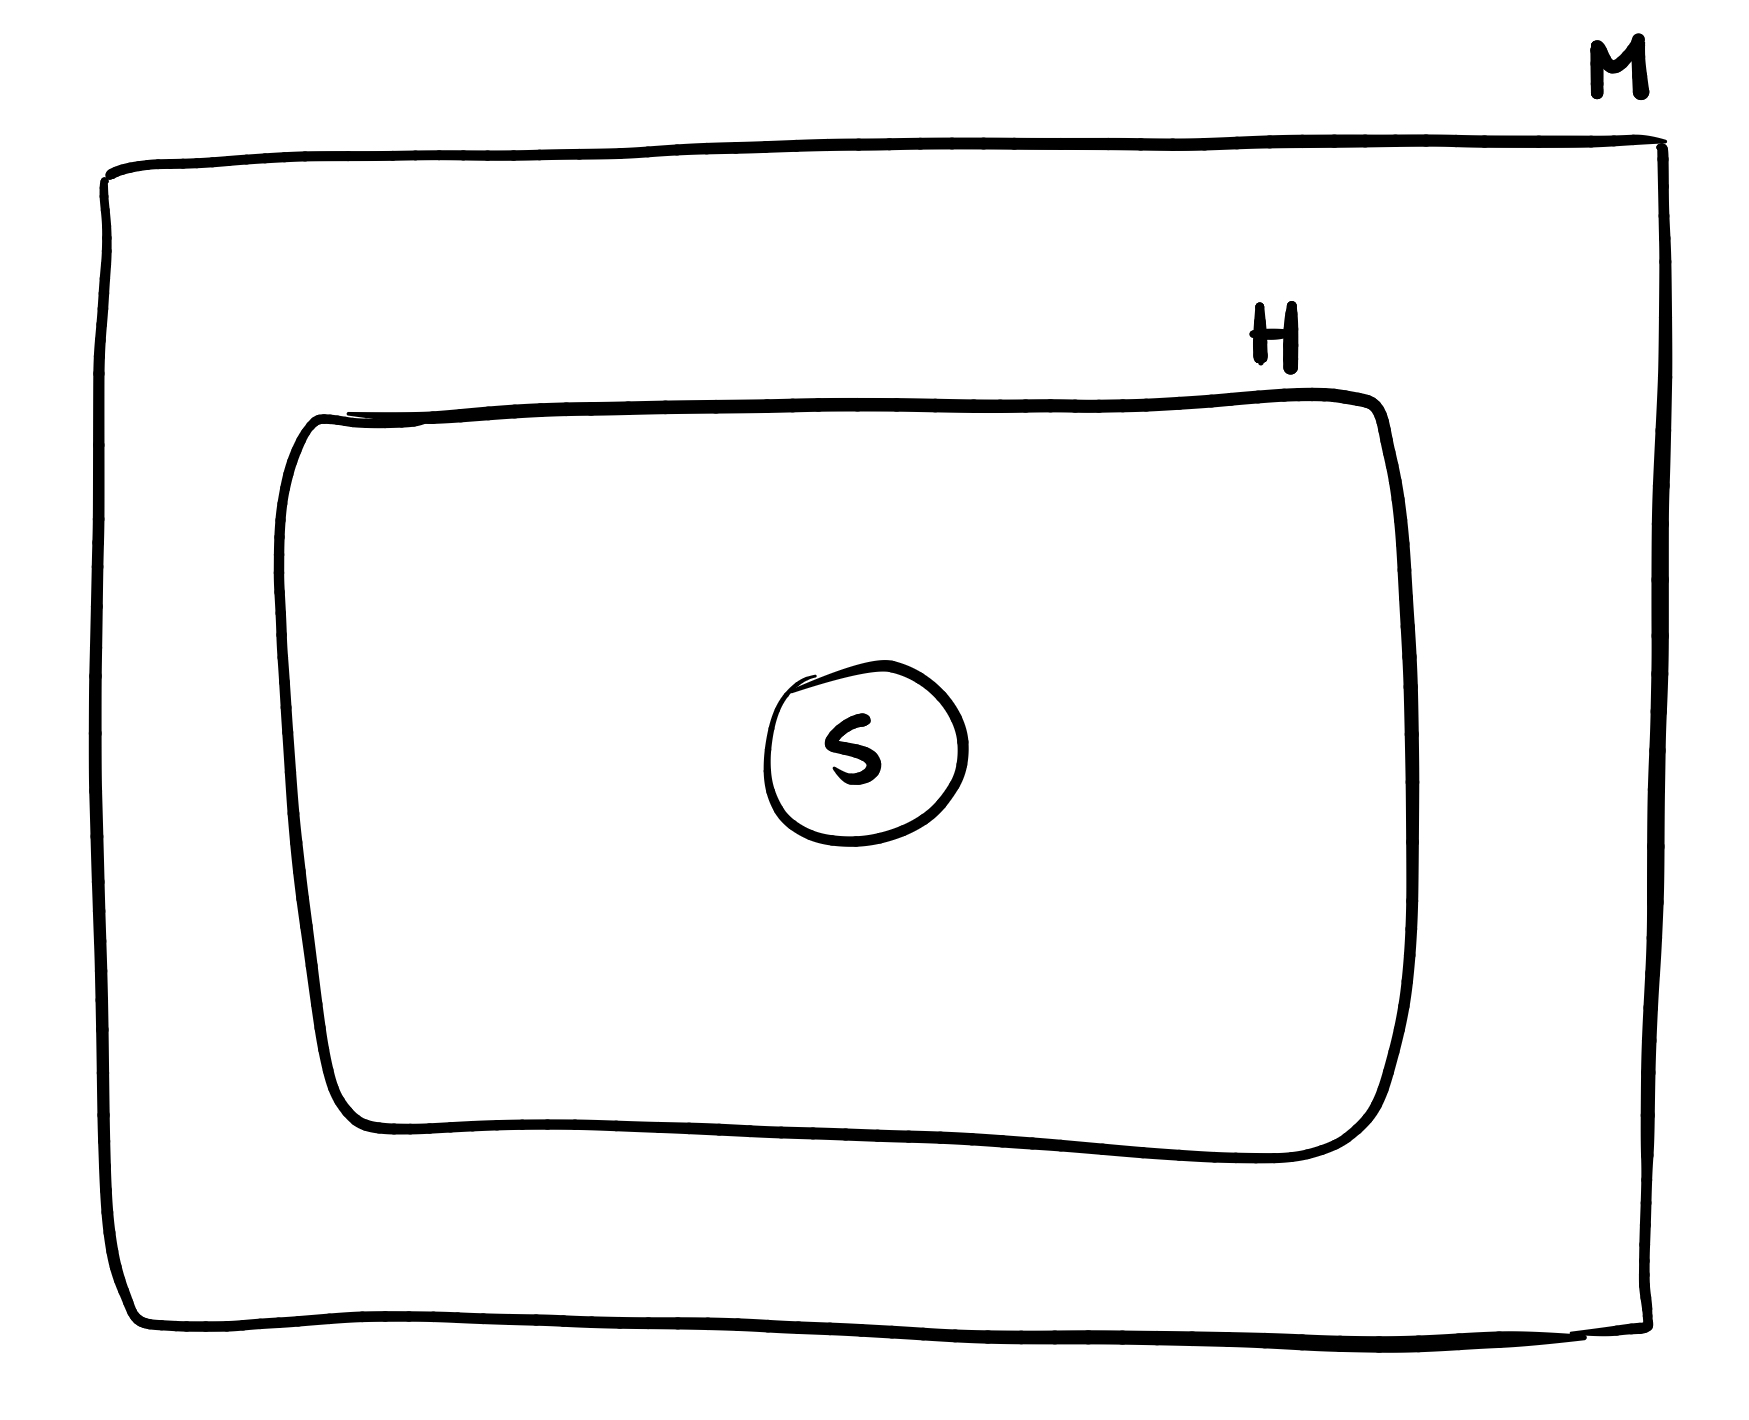
\includegraphics[scale=0.10]{imagensintro/socrates.jpeg}};
      \end{scope}
    \end{tikzpicture}
    \caption{Existe o grupo dos mortais, e a premissa P1 afirma que os homens fazem parte desse grupo. A premissa P2 afirma que Sócrates faz parte do grupo dos homens, logo, concluímos que Sócrates também faz parte do grupo dos mortais.}
    \label{intro06}
\end{figure}



Nessa analogia, as premissas seriam os princípios que fundamentam a nossa teoria física, e a conclusão seria uma equação matemática derivada de tais premissas, isto é, uma equação matemática que expressa uma conclusão lógica e irrefutável uma vez que se assume os princípios da teoria como verdadeiros. 

Poderíamos, por exemplo, criar uma teoria a respeito de como a luz se propaga. Tal teoria poderia enunciar, como princípio fundamental, que a luz se move de modo a sempre minimizar o tempo de percurso (o que de fato ocorre, e é conhecido como Princípio de Fermat, como veremos mais adiante). Além disso, poderíamos definir uma nova grandeza, o índice de refração $n$, de modo que seria possível construirmos o silogismo:

\begin{quote}
    P1: A luz se move de modo a sempre percorrer o trajeto que minimiza o tempo de percurso.\\
    P2: O índice de refração $n$ de um meio é definido como sendo $n := \sfrac{c}{v},$ em que $v$ é a velocidade da luz no meio e $c$ é a velocidade da luz no vácuo.\\
    C: Logo, ao mudar de meio, o comportamento da luz é governado pela equação matemática
    
    $$n_1 \sin \theta_1 = n_2 \sin \theta_2. $$
\end{quote}

Sim, eu sei: a conclusão não parece nada óbvia. Concluir que Sócrates era mortal foi muito mais fácil, mas acredite em mim: aqui estamos fazendo a mesma coisa. O fato de que a equação que governa a refração da luz --- ilustrada na Figura \ref{intro05} --- é aquela não ficou nada claro. Isso porque são necessários alguns passos intermediários de desenvolvimento matemático, o que será feito em momento oportuno. 


\begin{figure}[h]
    \centering
    \begin{tikzpicture}
      \begin{scope}[blend mode=multiply]
        \node {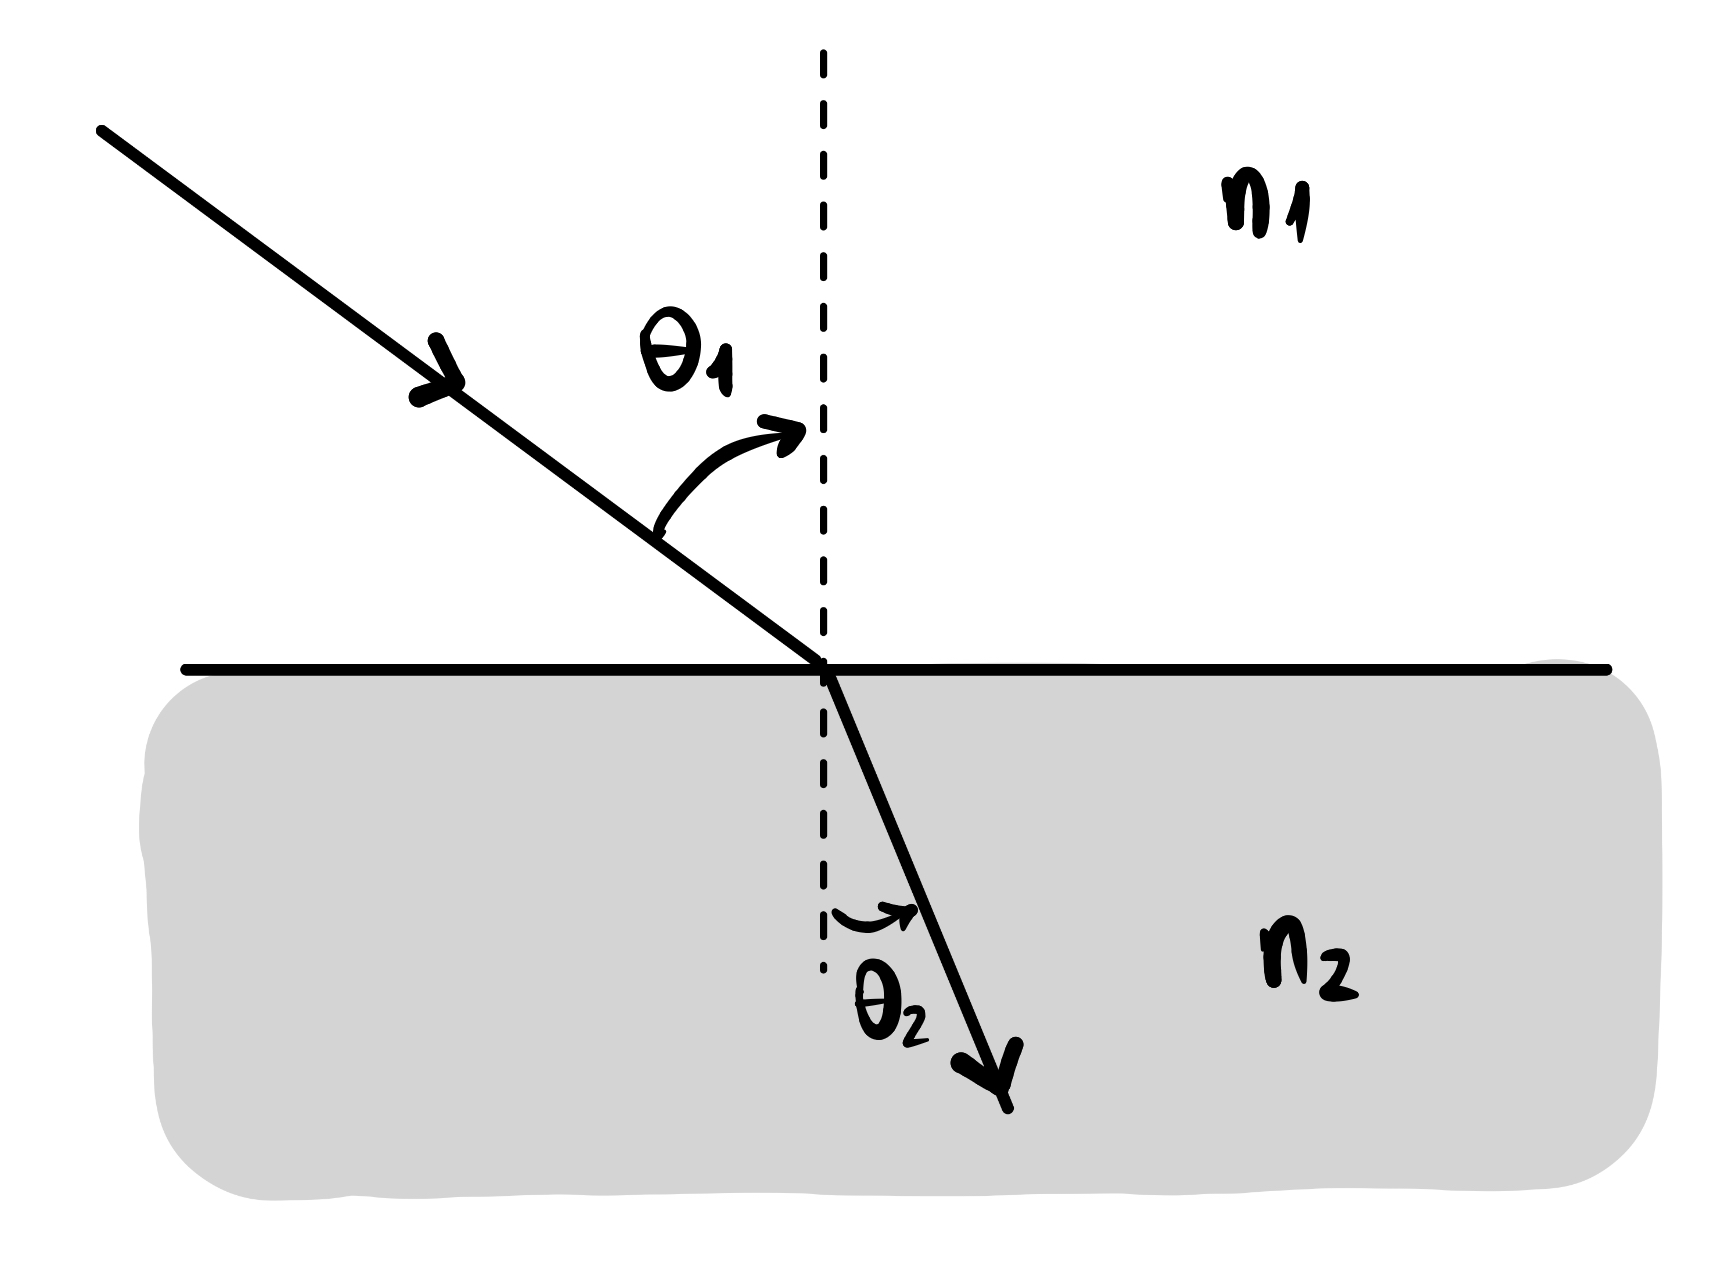
\includegraphics[scale=0.10]{imagensintro/refracao.jpeg}};
      \end{scope}
    \end{tikzpicture}
    \caption{Refração da luz.}
    \label{intro05}
\end{figure}

Contudo, para além da diferença no nível de dificuldade, o que foi feito acima é exatamente igual ao silogismo sobre a mortalidade de Sócrates. Assim, eis o nosso terceiro tipo de equação física: consequências lógicas e inevitáveis de termos assumido como verdadeiros os princípios da nossa teoria.

Tais equações, portanto, podem ser demonstradas, isto é, explicadas e construídas do zero com base nos pressupostos da teoria. Este é um tipo bem particular de equação, haja vista que as definições podem, no máximo, ser bem motivadas, mas elas são criações --- invenções humanas para estabelecer o vocabulário da teoria. Já as equações experimentais não têm nenhum tipo de margem para intervenção humana: elas são, letra por letra, governadas pelo experimento --- elas não dizem nada mais nada menos do que o experimento revelou. Já este terceiro tipo de equação, as demonstráveis, serão as que exigirão mais criatividade e arcabouço matemático, uma vez que elas são ``informações ocultas'' da teoria: elas estão ali, e dizem algo a respeito de como a natureza funciona, mas precisam ser encontradas e desvendadas, respeitando, naturalmente, as leis da lógica. Elas não estão explícitas, como as premissas, mas sim implícitas, e é preciso um olhar atento e refinado para conseguir extrair as conclusões que nos levarão a tais equações, que, como toda equação, apenas contém uma informação --- em linguagem matemática --- a respeito de como a natureza funciona.

Vejamos, a título de ilustração, algumas outras equações que são desse mesmo tipo.




\subsubsection{Período do Pêndulo Simples}

No século XVII, Galileu havia observado o \textit{isocronismo dos pêndulos de comprimentos idênticos,} ou seja, que pêndulos de mesmo comprimento sempre possuem o mesmo período de oscilação,\footnote{Do grego, \textit{iso = igualdade} e \textit{chronos = tempo}} independentemente da massa do objeto que está amarrada em sua extremidade. Ou seja, os três pêndulos da Figura \ref{intro06pend}, por terem o mesmo comprimento, terão exatamente o mesmo período de oscilação (tempo para que a massa vá de um extremo ao outro, retornando ao ponto inicial), independentemente dos valores das massas amarradas na sua extremidade.



\begin{figure}[h]
    \centering
    \begin{tikzpicture}
      \begin{scope}[blend mode=multiply]
        \node {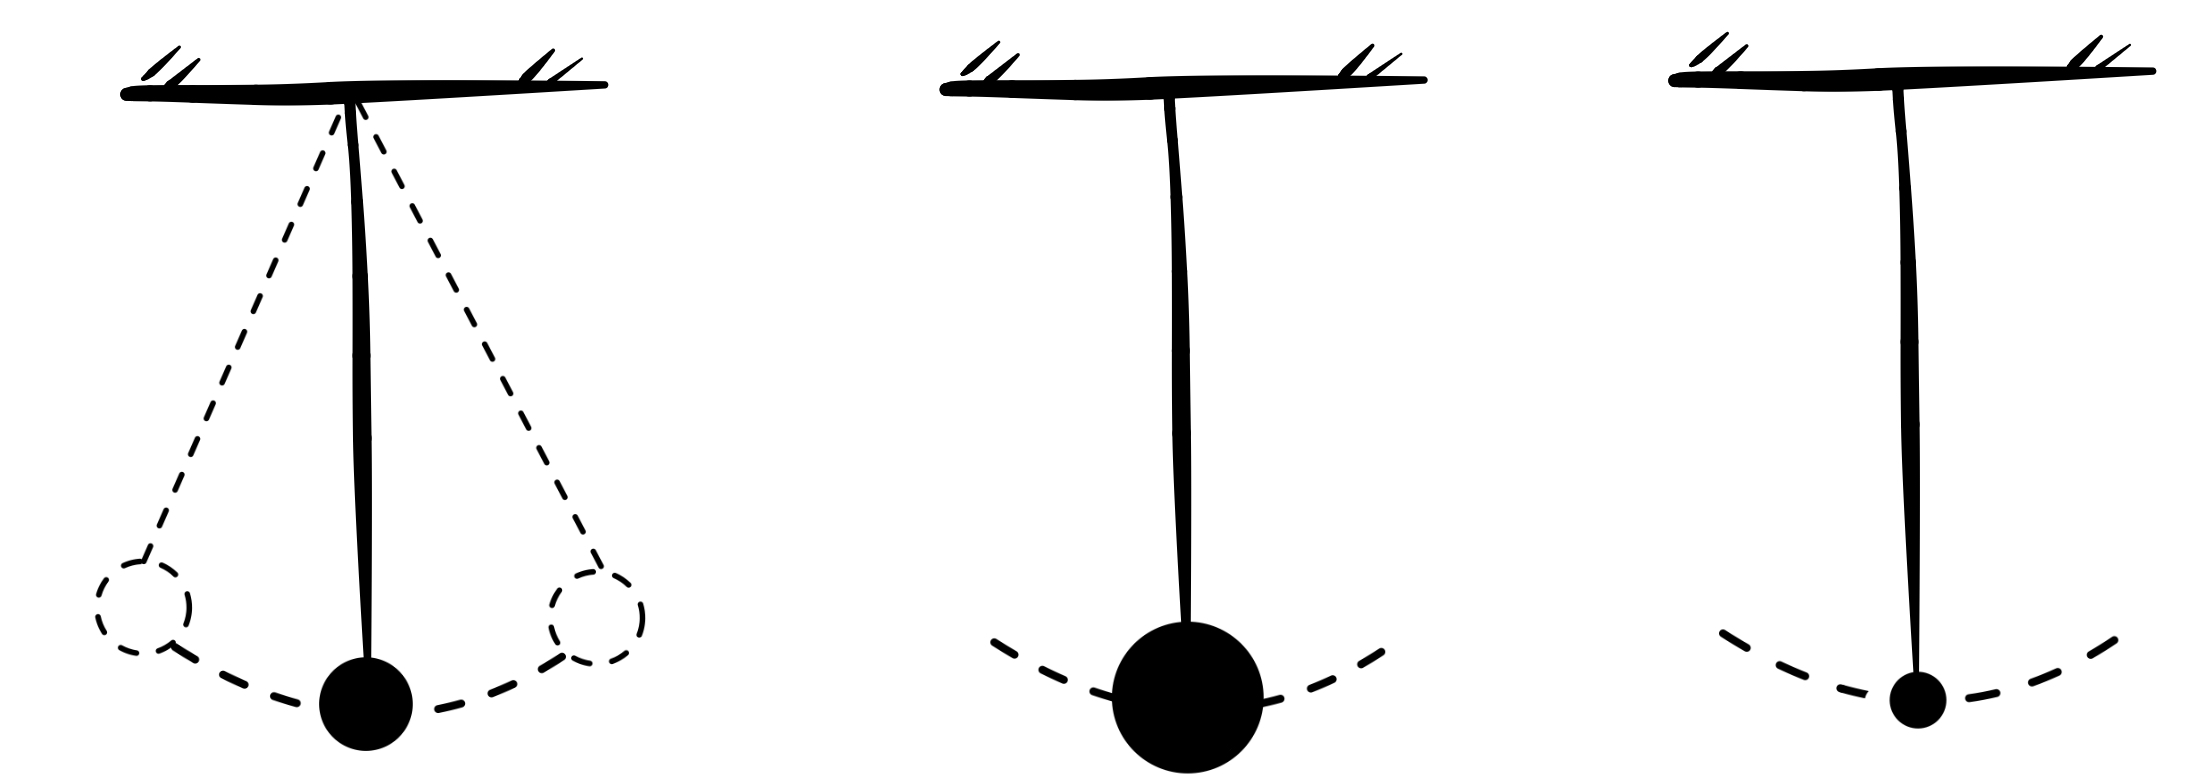
\includegraphics[scale=0.10]{imagensintro/pendulo.jpeg}};
      \end{scope}
    \end{tikzpicture}
    \caption{Oscilação do pêndulo simples.}
    \label{intro06pend}
\end{figure}


Que pêndulos de mesmo comprimento $l$ possuem o mesmo período de oscilação $T$, portanto, é um fato experimental. Contudo, podemos demonstrar, usando a teoria da dinâmica newtoniana e algumas premissas sobre o movimento oscilatório (não faremos isso neste momento) que o período de oscilação $T$ do pêndulo simples é dado por

\begin{equation}
    T = 2\pi \sqrt{\dfrac{l}{g}},
    \label{00intro_eq_pendulo}
\end{equation}
em que $g$ é a aceleração da gravidade e $l$ é o comprimento do pêndulo. Tal equação não é uma definição --- não estamos definindo nenhuma grandeza nova aqui --- e tampouco exprime simplesmente o resultado de algum experimento. Note que a equação, naturalmente, está de acordo com o experimento: o período depende do comprimento $l$ do fio, mas não da massa $m$ amarrada na sua extremidade, de modo que pêndulos de mesmo comprimento $l$ terão o mesmo período de oscilação qualquer que seja a massa amarrada em suas extremidades.

A Equação \eqref{00intro_eq_pendulo}, portanto, vai além: ela nos diz exatamente como pode-se calcular com precisão o período de um pêndulo simples qualquer\footnote{Para pequenas oscilações, como veremos em detalhes no estudo do volume II dessa coleção.}. Ela é uma consequência lógica dos princípios da teoria, expressando uma faceta a respeito de como a natureza funciona, no caso, como certos tipos de objetos oscilam sob a ação da gravidade. 

Tal equação, portanto, é uma conclusão (no sentido da lógica aristotélica): ela é uma consequência lógica dos pressupostos da teoria e, naturalmente, nos diz algo a respeito do funcionamento do universo. O fato do experimento concordar com o que tal conclusão diz é um bom indicativo de que as premissas da teoria devem estar corretas.

Quais são as premissas e como é o desenvolvimento lógico para nos permitir tirar a conclusão e desaguar na Equação \eqref{00intro_eq_pendulo} é algo que será feito em um momento futuro. Por hora, é importante que o leitor entenda apenas a diferença entre esse novo tipo de equação e os dois tipos anteriores.




\subsubsection{Equação Fundamental da Ondulatória}

Este é um exemplo de natureza mais simples, de modo que faremos seu desenvolvimento completo, para tentar trazer mais clareza ao leitor sobre esse tipo de equação.

Dada uma onda de \textit{comprimento de onda} $\lambda$ (isso é uma definição: criação de vocabulário para nos permitir construir a teoria), frequência $f$ (também uma definição) e velocidade de propagação $v,$ como mostra a Figura \ref{introonda}, essas três grandezas se relacionam por meio da Equação Fundamental da Ondulatória, que estabelece que

\begin{equation}
    v = \lambda f.
    \label{00intro_eq_vlambdaf}
\end{equation}

\begin{figure}[h]
    \centering
    \begin{tikzpicture}
      \begin{scope}[blend mode=multiply]
        \node {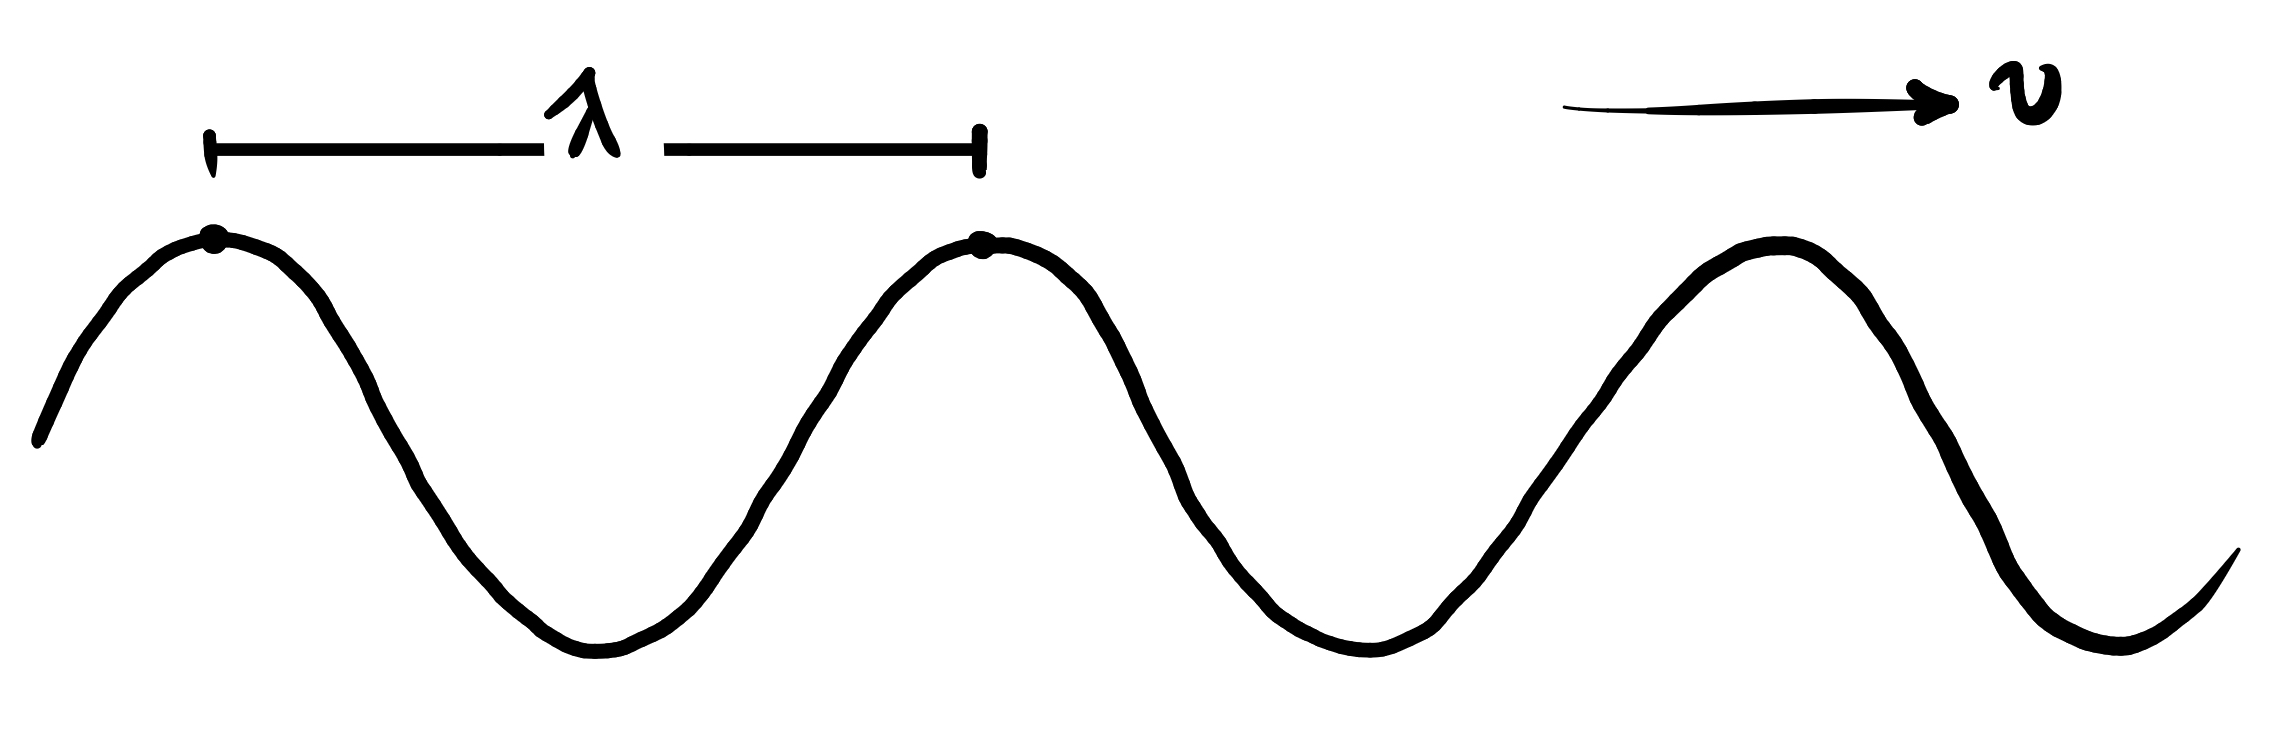
\includegraphics[scale=0.10]{imagensintro/onda.jpeg}};
      \end{scope}
    \end{tikzpicture}
    \caption{Propagação da onda.}
    \label{introonda}
\end{figure}


A Equação \eqref{00intro_eq_vlambdaf} não é resultado de um experimento, tampouco serve para definir alguma grandeza. Ela é uma consequência lógica do que é estabelecido pela teoria. 

Podemos demonstrá-la a partir da equação básica da Cinemática que define a velocidade média --- a Equação \eqref{00intro_eq_velocidade}.


\vspace{0.3cm}
{
\centering
\begin{tikzpicture}
  \begin{scope}[blend mode=multiply]
    \node {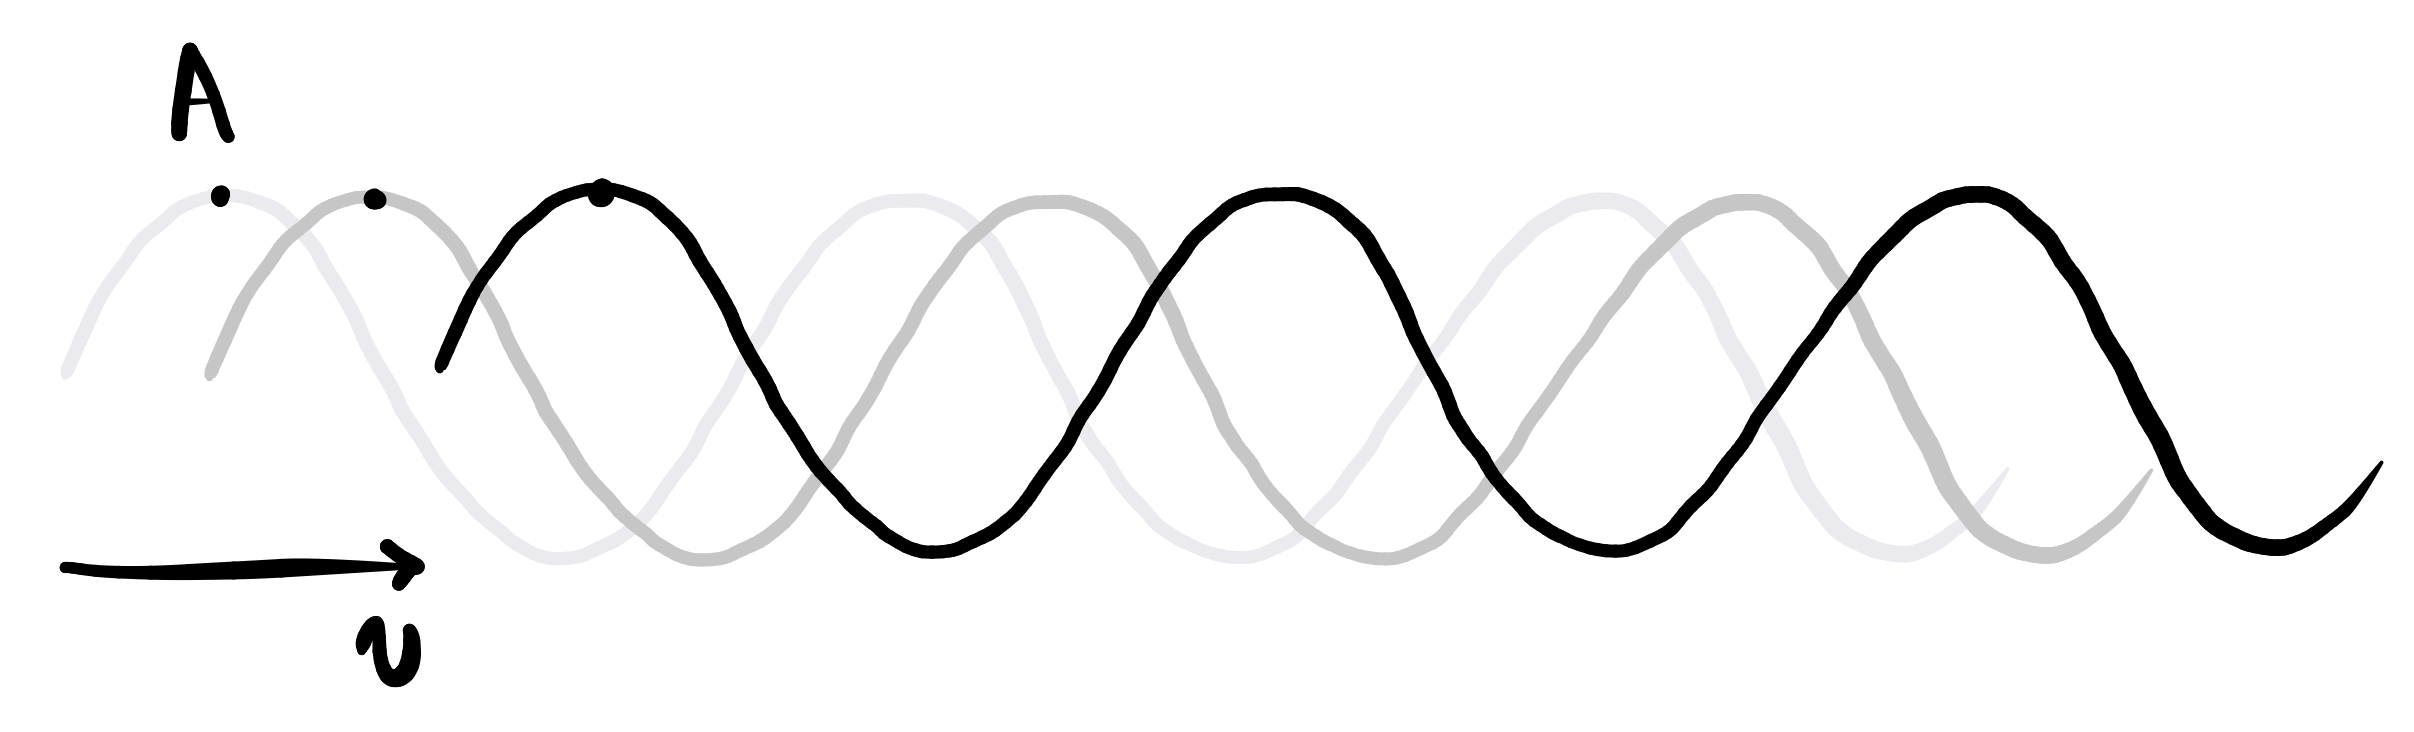
\includegraphics[width=0.8\linewidth]{imagensintro/ondapropagando.png}};
  \end{scope}
\end{tikzpicture}
\captionof{figure}{Onda se propagando para a direita.}
\label{fig_intro_ondapropagando}
} 
\vspace{0.3cm}


A Figura \ref{fig_intro_ondapropagando} mostra diferentes instantes da propagação de uma onda. Observe que o ponto $A$ destacado é sempre o mesmo, ele apenas está representado em diferentes instantes de tempo. Sendo $T$ o tempo de um período (um ciclo da onda) e sendo $\lambda$ definido como a distância que a onda percorre em um ciclo, ou seja, em um período, segue que, ao longo de tal intervalo de tempo, teríamos:

\begin{align}
    d &= vt,  \nonumber \\
    \lambda &= vT, \nonumber
\end{align}
ou seja, no tempo de um período $T$ a distância percorrida será igual a um comprimento de onda, $\lambda.$ Sendo a frequência $f$ dada pelo inverso do período $T$ (outra definição), teremos

$$ \lambda = vT \implies \lambda = v \dfrac{1}{f} \implies \boxed{v = \lambda f.}$$


Ou seja, tal equação é uma verdade fundamental sobre o comportamento das ondas, mas obtida não por meio do experimento, mas sim por meio de explorar a teoria e tentar entender o que decorre logicamente dos seus pressupostos, ou seja, quais são as ``verdades ocultas'', isto é, implícitas, contidas na teoria. Caso o leitor queira entender em um pouco mais de detalhes cada passo lógico usado, fizemos algo como o que segue abaixo:

\begin{quote}
    P1: O comprimento de onda $\lambda$ de uma onda é a distância que tal onda percorre ao longo de um ciclo.\\
    P2: A frequência $f$ de uma onda é dada pelo número de oscilações de tal onda por unidade de tempo.\\
    P3: O período $T$ de uma onda equivale ao tempo para que ela complete um ciclo de oscilação, e é dado pelo inverso da frequência.\\
    P4: A velocidade de propagação da onda é constante, de modo que vale a equação $d=vt.$\\
    C: A onda deve satisfazer a equação $\boxed{v = \lambda f.}$

\end{quote}

O desenvolvimento matemático para se tirar tal conclusão e desaguar na equação destacada é o que foi feito anteriormente.

Faz-se mister destacar ao leitor que a equação $v=\lambda f$ não é a definição de velocidade de uma onda, e sim uma relação que deve ser satisfeita por qualquer tipo de onda, por consequências lógico-matemáticas da forma como se define o comprimento de onda $\lambda$ e a frequência $f.$ A velocidade de uma onda depende, na verdade, das características do meio em que ela se propaga. Por exemplo, para uma onda se propagando em uma corda, sua velocidade é dada pela Equação de Taylor:

$$ v = \sqrt{\dfrac{F}{\mu}},$$

\noindent em que $F$ e $\mu$ representam a tração na corda e sua densidade linear, respectivamente. Estudaremos em detalhes tal equação em um momento futuro. Por hora, é importante notar que, ainda que a velocidade da onda na corda dependa do tipo de corda ($\mu$) e da força de tração na corda ($F$), ela também deve, necessariamente, ser igual ao produto $\lambda f.$ Ou seja, o comprimento da onda naquela corda, sua frequência e a velocidade de propagação dada pela Equação de Taylor devem ser tais que a equação $v=\lambda f$ seja satisfeita.








\section{Um passeio pelas equações}

A introdução feita até aqui é, possivelmente, a parte mais importante de todo este livro. Isso porque, caso o leitor não esteja disposto a ampliar seu horizonte e visualizar as equações matemáticas como informações --- que devem, portanto, ser compreendidas e não meramente memorizadas --- será muito difícil prosseguirmos juntos nessa jornada.

As páginas que se seguem buscarão mostrar todas as equações da Física sob a óptica que apresentamos aqui: vamos entender qual tipo de equação se trata, qual é o papel que aquela equação ocupa e qual é a informação que ela carrega. Em momento algum vamos simplesmente apresentar uma equação, entregar para o leitor um pequeno macete mnemônico para facilitar sua memorização e lhe ensinar como usar a equação para resolver algum problema. 

Eu entendo que, possivelmente, esse tenha sido o caminho trilhado até aqui pelo leitor, mas esse não é um livro que se propõe a fazer mais do mesmo. Se  deseja quebrar esse ciclo vicioso de ``aprendizado'', é preciso que esteja preparado para o momento de ruptura. Dito isso, incentivo o leitor a retornar, caso necessário, nas seções anteriores desta introdução, caso algo não tenha sido bem compreendido. É certo que algumas coisas que discutimos aqui vão se tornar mais claras à medida que avançarmos no texto e aplicarmos tal método em diferentes equações, contudo, é importante que o leitor tenha compreendido o panorama geral antes de iniciarmos este nosso passeio pelas equações da Física.

Parece relevante também comentar a respeito da escolha das equações que serão apresentadas e a ordem em que as apresentaremos. Este é um texto voltado para o estudante do Ensino Médio, de modo que todas as equações que trataremos serão aquelas trabalhadas e apresentadas neste contexto. Além disso, este material não se propõe a esgotar integralmente todas as equações da Física que podem ser estudadas no Ensino Médio: escolhemos, intencionalmente, deixar algumas de fora, a fim de dar espaço para que o leitor possa, posteriormente, por si só, aplicar o método aqui aprendido e construir o entendimento de algumas outras equações. Trabalharemos, portanto, com as principais equações --- as mais clássicas e relevantes de cada tópico --- de modo a passar por todas as áreas da Física, varrendo as suas partes mais relevantes.

Por fim, poderíamos escolher apresentar as equações em blocos de três grupos --- sendo cada grupo um tipo de equação, como enunciamos anteriormente. Contudo, pareceu muito mais didático apresentar as equações organizadas por assuntos, de modo que o texto ficará dividido em três grandes partes:

\begin{itemize}
    \item [(i)] Mecânica.
    \item [(ii)] Óptica, Ondas e Termodinâmica.
    \item [(iii)] Eletromagnetismo.
\end{itemize}

É muito importante que o material seja estudado na ordem cronológica em que é apresentado. Tal ordem foi cuidadosamente escolhida a fim de que cada nova ideia dependa exclusivamente de ideias e conceitos anteriormente construídos. Assim, a experiência e eficiência da aprendizagem será tão mais eficiente quanto mais fiel o leitor se mantiver à ordem de estudos aqui apresentada.

% Este é um material que deve ser usado em paralelo com um curso de Física para o Ensino Médio: quando o leitor estiver estudando, digamos, Hidrostática, ele deve consultar, na parte de Mecânica, a seção sobre tal tema, na qual apresentaremos e destrincharemos as principais equações de tal assunto.

Este material, portanto, não se propõe a ser um material didático completo para se aprender Física, mas sim um material de apoio, que irá apresentar, por uma perspectiva única, as principais fórmulas que se estudam em Física. Na seção sobre Hidrostática, por exemplo, não nos propomos a construir toda a teoria, apresentar todos os conceitos e passar por toda a história de tal tópico. Partiremos da premissa de que isso já foi feito pelo estudante, e, usando tal arcabouço conceitual, vamos apresentar e destrinchar cada equação matemática que se estuda dentro de tal assunto.

Deixamos ao leitor a sugestão de considerar construir tal arcabouço teórico pelo curso Lições de Física, ministrado pelo próprio autor que vos escreve, e disponível na escola on-line Universo Narrado. As próprias seções deste livro foram organizadas com base nos módulos e aulas do curso, de modo a tornar mais fluido e didático o estudo daquele que está fazendo o curso e buscando destrinchar melhor cada fórmula por este material. 



\section{A Mecânica em História}

Como dito, essa é uma coleção que se dividirá em três volumes, sendo este --- o primeiro deles --- sobre Mecânica, e não poderia ser de outra forma.

A mecânica é o ramo da física que estuda como os corpos se movem e por que se movem. Ela busca descrever, por meio de conceitos e fórmulas, as regularidades do movimento dos objetos, desde uma pedra lançada ao ar até o movimento dos planetas. O experimento de se abandonar uma pedra e analisar seu movimento, como fizemos na Figura \ref{intro02}, é algo que a Mecânica se propõe a estudar e analisar.

A Mecânica é uma estrutura conceitual que relaciona:

\begin{itemize}
    \item posição,
     \item tempo,
      \item velocidade,
       \item força,
        \item massa,
         \item momento linear,
          \item torque,
         \item energia.
\end{itemize}


Historicamente, foi o primeiro grande campo da física a adquirir forma matemática rigorosa, sobretudo a partir do trabalho de Galileu e Newton. Por isso, ela serve como porta de entrada natural para o estudo da física como ciência teórica. A maior parte do que se desenvolveu na Física nos três séculos após Newton foi baseada na sua teoria mecânica --- por isso, começaremos por aqui: a base e o alicerce de quase toda a Física.

Neste livro, apesar da sua abordagem, a mecânica não será apresentada como um catálogo de fórmulas, mas como um sistema coerente de ideias, no qual cada equação tem um papel bem definido: algumas introduzem conceitos, outras descrevem regularidades experimentais, e muitas são consequências lógicas dos princípios adotados. Compreender a mecânica é compreender o primeiro grande exemplo de como a natureza pode ser organizada em linguagem matemática.

Mais do que apresentar ao leitor as fórmulas da mecânica, este livro se propõe a contar uma história. A Física, como toda grande narrativa, tem uma estrutura dramática. E se tivéssemos que contar a história da Mecânica --- a maneira como a humanidade aprendeu a descrever o movimento --- ela se desenrolaria naturalmente em três atos.

No \textbf{Primeiro Ato}, aprendemos a \textit{descrever} o movimento. Antes de perguntar por quê os corpos se movem, precisamos ser capazes de dizer, com precisão, \textit{como} eles se movem: onde estão, quão rápido vão, em que direção. É a Cinemática --- a linguagem do movimento, sem julgamentos sobre suas causas.

No \textbf{Segundo Ato}, aprendemos a \textit{explicar} o movimento. Entra em cena a força --- e com ela, Newton. A pergunta já não é apenas \textit{como}, mas \textit{por quê}: o que faz um corpo acelerar, o que o faz parar, o que conserva seu estado. É a Dinâmica --- e com ela surgem também energia, trabalho e impulso, as importantes quantidades conservadas que a natureza parece prezar acima de tudo.

No \textbf{Terceiro Ato}, colhemos os frutos. Com a linguagem e a teoria em mãos, voltamos nosso olhar para o mundo: a gravidade que governa planetas e projéteis, os fluidos que sustentam navios e balões. São as Aplicações --- onde a teoria encontra a realidade e demonstra seu poder.

Três atos, portanto, para contar uma única história: a de como a humanidade aprendeu a ler o livro da natureza. Comecemos, então, nosso mergulho nesse drama.





\paginailustracaoato{imagens_artes/galileuactone.png}

\part{Cinemática}
\epigrafeato{%
  Meu objetivo é expor uma ciência muito nova que trata de um
  tema muito antigo. Talvez nada na natureza seja mais antigo
  que o movimento\ldots%
}{Galileo Galilei}

    
% !TeX spellcheck = pt_BR

\chapter*{Do que se trata a Cinemática}
\addcontentsline{toc}{chapter}{Do que se trata a Cinemática}



%Escrever aqui uma boa intro sobre o que se trata a cinemática, e que tal estudo aqui ficará dividido em duas partes: a parte unidimensional, que é escalar, e a parte bidimensional, que é vetorial.





A Cinemática é a área da física que trata do estudo do movimento. Buscamos aqui compreender as relações entre movimentos de um corpo em relação a outro, da rapidez com que um objeto se move e do quanto sua velocidade aumenta ou diminui.

Por ora vamos analisar o movimento dos corpos de forma pura, sem se preocupar com o que causa tal movimento. Historicamente, foi pela Cinemática que a Física começou a se formar, com os estudos de Galileu sobre a queda dos corpos e o movimento dos projéteis, buscando entender como tais movimentos poderiam ser descritos, sem se preocupar com o que causava tais movimentos -- as forças.

Ao suspender, provisoriamente, a discussão sobre forças, a Cinemática permite construir uma linguagem precisa para falar de movimento. Essa separação não é artificial: antes de explicar o mundo, é preciso aprender a descrevê-lo, e é isso que faremos por meio deste estudo.

O nosso estudo se dividirá em duas partes: a Cinemática Escalar, que tratará essencialmente dos tipos mais simples de movimento: os movimentos unidimensionais. Neste contexto, como teremos uma única dimensão na qual o movimento pode ocorrer, o caráter vetorial de grandezas como velocidade e aceleração poderá ficar de lado, haja vista que, para um corpo que se move horizontalmente, restam-nos duas opções para onde ele pode estar se movendo: para a direita ou para a esquerda. Essas duas opções podem ser distinguidas por meio de uma atribuição de sinais: uma velocidade positiva pode representar um corpo se movendo para direita, enquanto uma velocidade negativa representaria um corpo que se move para esquerda.

Dessa forma, usando alguns artifícios algébricos como este, poderemos estudar em detalhe diversos tipos de movimentos em uma dimensão sem necessariamente precisar fazer um tratamento vetorial das grandezas cinemáticas envolvidas -- essa é a Cinemática Escalar.

Posteriormente, quando quisermos estudar movimentos bidimensionais ou mesmo tridimensionais, seremos obrigados a usar o tratamento vetorial: existem apenas dois tipos de sinais -- positivo ou negativo -- porém a velocidade agora pode apontar para uma infinidade de direções distintas, que não poderão mais ser diferenciadas apenas com a atribuição de um sinal algébrico. Com isso, adentraremos no estudo da Cinemática Vetorial, em que redefiniremos todas as grandezas outrora estudadas na Cinemática Escalar, porém agora dando o devido tratamento vetorial a elas. Essa parte começará com uma breve apresentação sobre os vetores, suas características geométricas e suas operações. Com isso, estaremos munidos de todas as ferramentas necessárias para descrever a evolução de qualquer tipo de movimento -- e teremos, em mãos, tudo que precisamos para avançar nos estudos da Dinâmica, que constitui a segunda parte do nosso estudo.








% !TeX spellcheck = pt_BR

\chapter{Cinemática Escalar}

Neste capítulo, estudaremos os movimentos mais simples que a natureza oferece: aqueles que ocorrem em uma única dimensão — ao longo de uma reta. Como discutimos na introdução desta parte, essa restrição nos permite tratar as grandezas cinemáticas de forma algébrica, sem recorrer ao formalismo vetorial: uma velocidade positiva indica que o corpo se move em um sentido; uma velocidade negativa, no sentido oposto. É esse artifício simples que justifica o nome Cinemática Escalar.



O capítulo começa pelos conceitos fundamentais — velocidade escalar média e aceleração escalar média —, que são definições: acordos sobre como expressar, com precisão, o quão rápido um corpo se move e o quão rapidamente essa rapidez muda. A partir delas, derivamos as equações que descrevem os dois movimentos retilíneos mais importantes da mecânica clássica: o Movimento Uniforme (MU), em que a velocidade é constante, e o Movimento Uniformemente Variado (MUV), em que a aceleração é constante. As equações horárias da posição e da velocidade, a equação de Torricelli e a expressão da velocidade média no MUV formam o núcleo desse estudo.



O que o leitor encontrará aqui não é uma lista de fórmulas para decorar, mas a história de como cada uma delas surge naturalmente da anterior — cada equação demonstrável sendo deduzida a partir das definições e das equações que a precedem. Ao fim deste capítulo, o leitor terá em mãos não apenas as ferramentas para resolver problemas de cinemática escalar, mas também a compreensão de por que essas ferramentas funcionam.






\newpage


\section{Conceitos Introdutórios}


\begin{secnivel}[Velocidade Escalar Média]{I}{Velocidade Escalar Média}
  
  \eqLdois{def}{mecanica_eq_velocidademedia}{v_m := \dfrac{\Delta s}{\Delta t}}

\end{secnivel}





\secgfe{De onde vem}

Ao longo da introdução, na seção \ref{subsecao_introducao_eqsdefinicoes}, já discutimos amplamente qual é a razão de criarmos o conceito de velocidade e defini-lo como fizemos, de modo que ficaria demasiadamente repetitivo trazer de novo tal discussão aqui. Dito isso, vale destacarmos uma pequena diferença entre a definição de velocidade média que lá fizemos e a que foi feita aqui, por meio da Equação \eqref{mecanica_eq_velocidademedia}. 


    \begin{figure}[h]
    \centering
    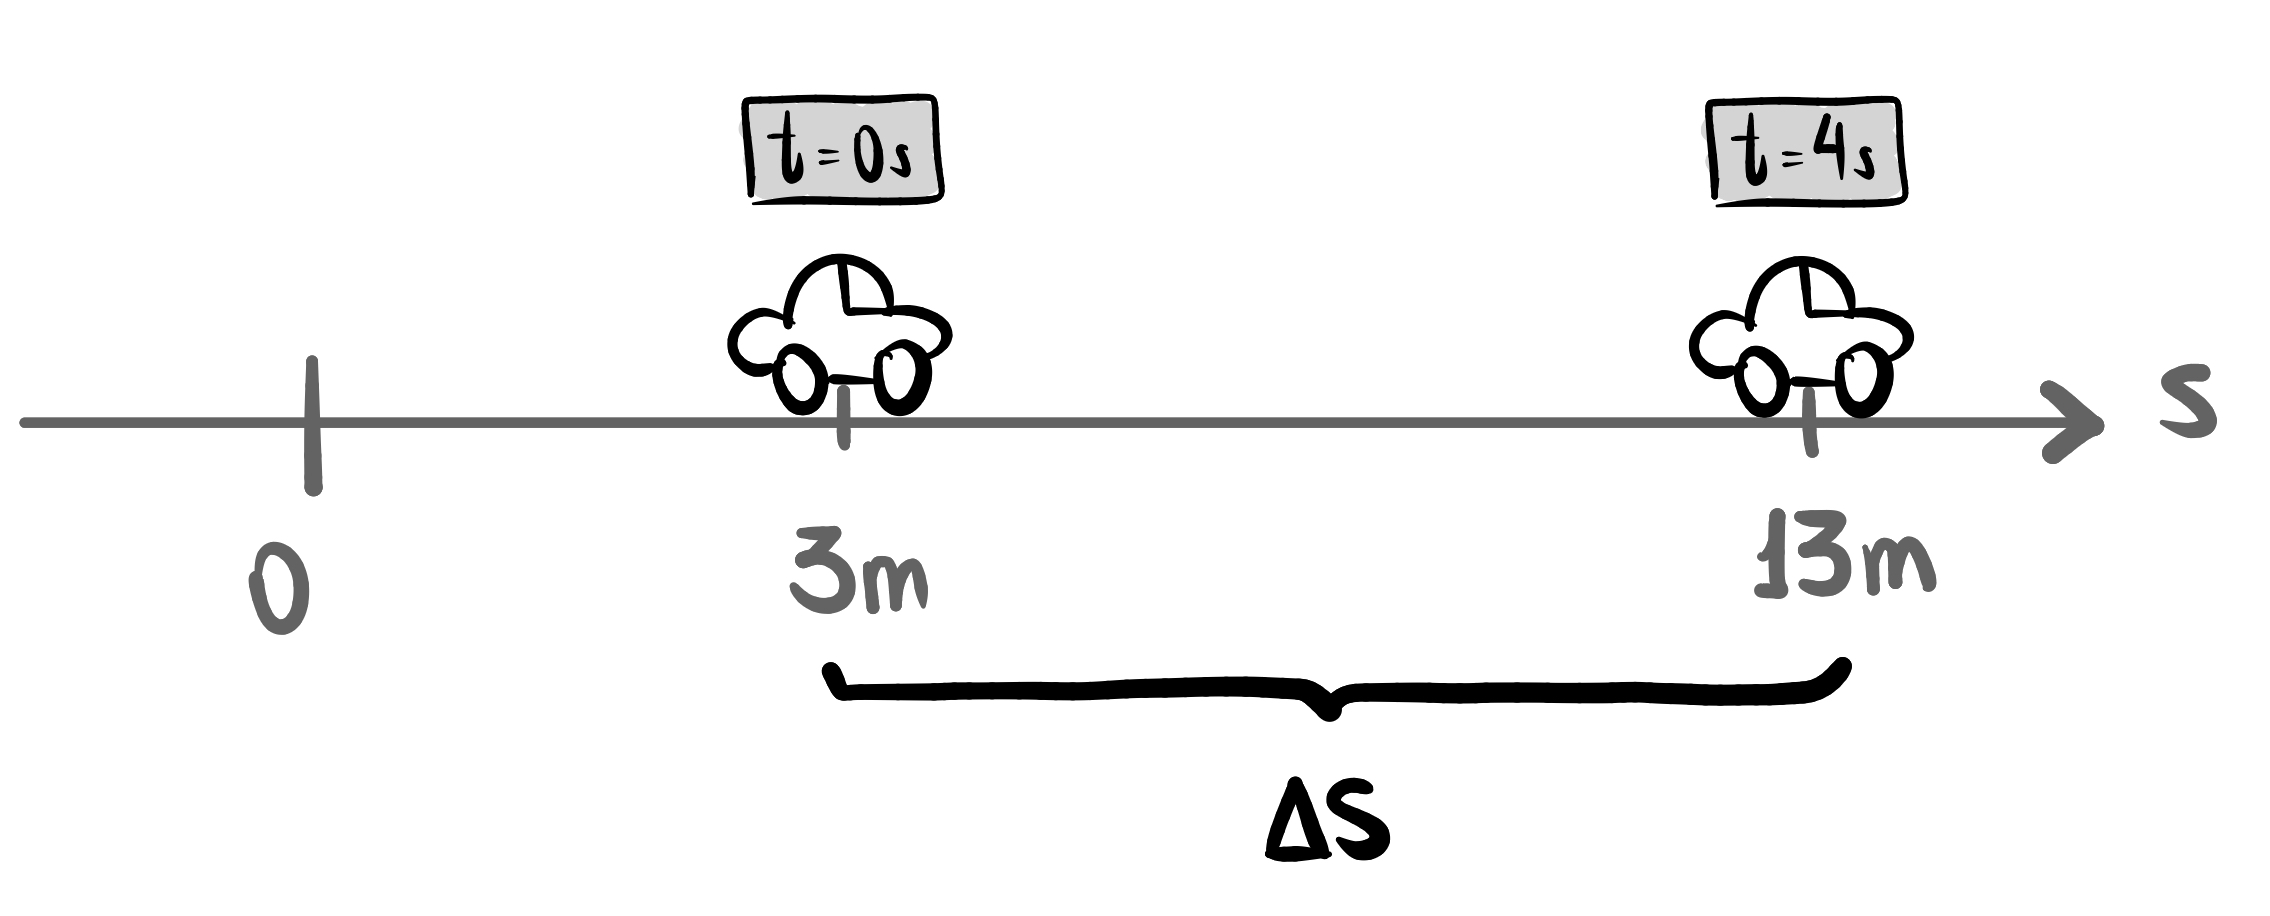
\includegraphics[scale=0.135]{imagensmecanica/deslocamentoescalar.jpeg}
    \caption{Deslocamento $\Delta s.$}
    \label{fig_mec_deslocamento_escalar}
\end{figure}

A bem da verdade, aquela forma de definir a velocidade, feita na introdução, não está exatamente correta -- ou, pelo menos, está incompleta --, por isso vamos refiná-la neste momento. Para medirmos um movimento é preciso que se saiba aonde o objeto está em cada instante de tempo -- é por isso que as estradas possuem placas de quilometragem: caso o seu carro quebre, você pode acionar o guincho e dizer que está no quilômetro 173 da BR-XYZ. 

Em Física, fazemos isso por meio da definição de um eixo de posições $s$, com uma origem -- a posição zero, a partir da qual começamos a medir --, e uma orientação: para onde as posições crescem. A Figura \ref{fig_mec_deslocamento_escalar} mostra isso, em que um carro começa na posição inicial $s_0=3$m, avançando para a posição final $s_f=13$m, ao longo de 4 segundos. A diferença entre a posição inicial e final é o que chamamos de deslocamento escalar $\Delta s$, dado por $\Delta s = s_f - s_0$, e com base nele definimos a velocidade média: ela é a razão entre o deslocamento escalar $\Delta s$ e o intervalo de tempo $\Delta t$ ao longo do qual tal deslocamento acontece.

Dito tudo isso, o leitor poderia se perguntar: \textit{mas isso não é a mesma coisa que a distância?}

E a resposta é: nem sempre. É claro que no caso da Figura \ref{fig_mec_deslocamento_escalar}, as duas coisas coincidem: o carro percorreu uma distância de 10m, e seu deslocamento escalar foi de $\Delta s = s_f-s_0 = 13 - 3 = 10 $m. O deslocamento, da forma como definimos, mede o resultado líquido do movimento, ou, caso o leitor prefira, o efeito global do movimento. A Figura \ref{fig_mec_deslocamento_vs_distancia02} deixa isso mais evidente: ela representa o movimento de um carro que sai da posição inicial $s_0=3$m, se desloca até a posição $13$m e depois retorna até a posição final $s_f=8$m. A distância total percorrida, naturalmente, foi a soma das distâncias varridas na ida e na volta, totalizando $10+5=15$ metros, porém o deslocamento escalar foi $\Delta s = s_f-s_0=8-3=5$ metros.\footnote{Podemos definir a distância percorrida como sendo $d= |\Delta s_{\text{ida}}| + |\Delta s_{\text{volta}}|,$ de modo que a distância percorrida será sempre positiva, diferente do deslocamento.}

Veja que a distância percorrida leva em conta, de fato, o comprimento da trajetória do corpo, enquanto que o deslocamento escalar -- posição final menos inicial -- irá medir o quanto o corpo se afastou do seu ponto de partida, ou seja, o efeito ``líquido do movimento''. Note que em todos os casos nos quais \textbf{não há inversão no sentido do movimento}, ou seja, o objeto sempre avança no mesmo sentido, a distância e o deslocamento escalar irão sempre coincidir -- e boa parte dos movimentos que estudaremos aqui estarão nesse contexto. Ou seja, nesses casos, as Equações \eqref{00intro_eq_velocidade} e \eqref{mecanica_eq_velocidademedia} serão equivalentes. O deslocamento escalar e a distância foram diferentes no caso da Figura \ref{fig_mec_deslocamento_vs_distancia02} justamente pelo fato de que o carro mudou o sentido de seu movimento.

 \begin{figure}[h]
    \centering
    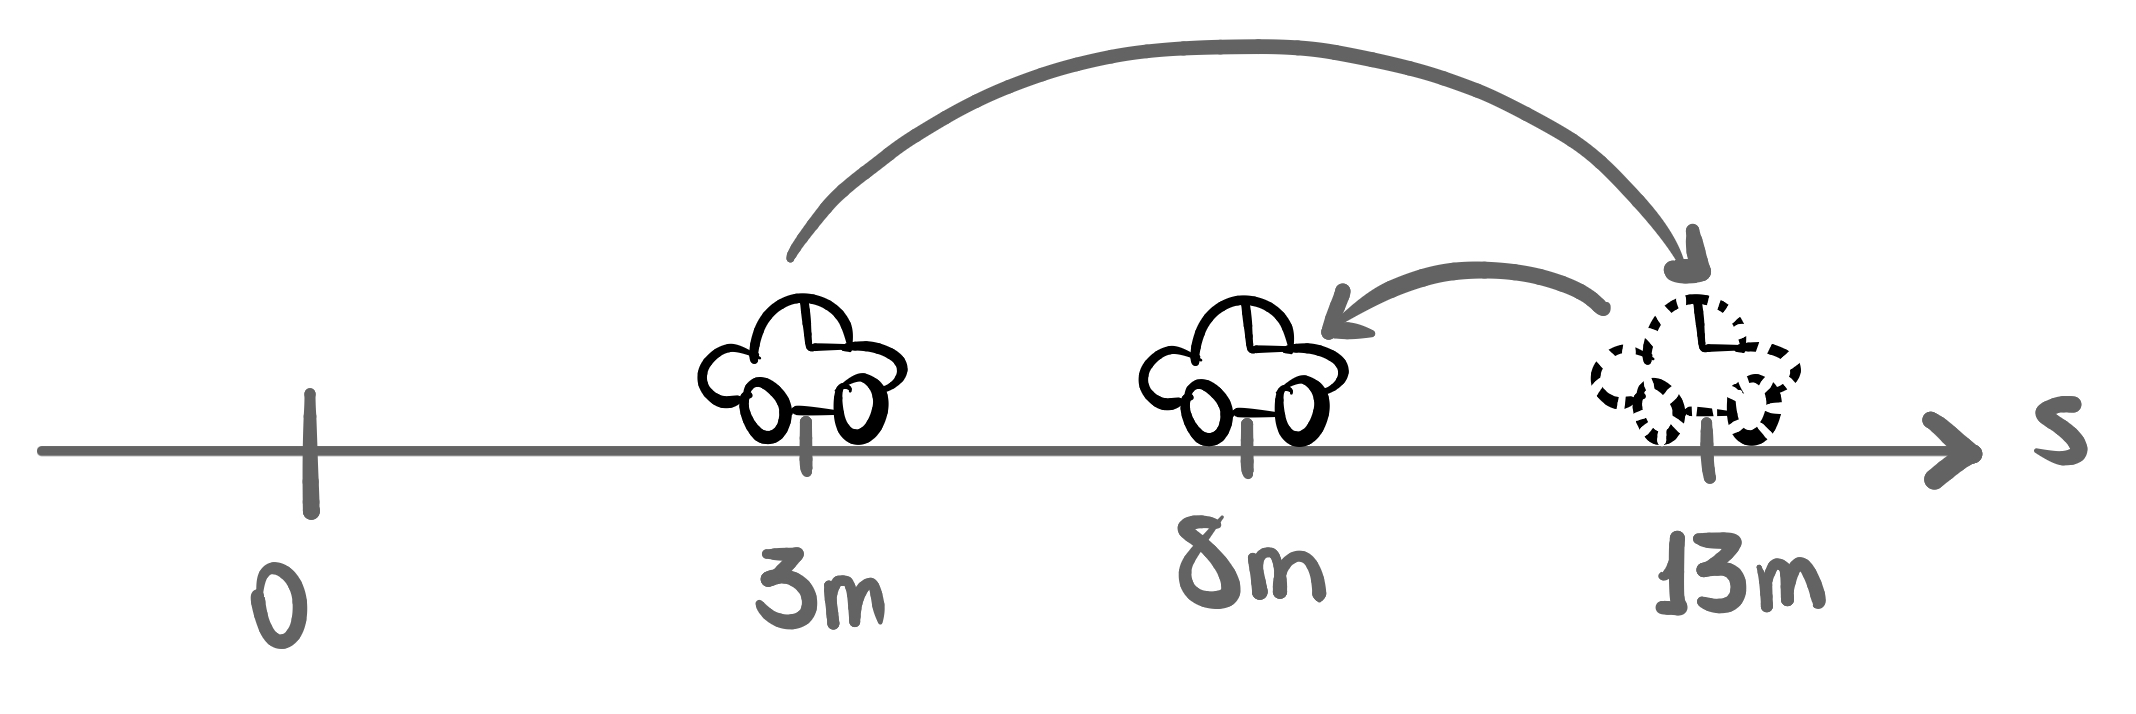
\includegraphics[scale=0.12]{imagensmecanica/deslocamentoescalarn.jpeg}
    \caption{A diferença entre o deslocamento $\Delta s$ e a distância percorrida $d$.}
    \label{fig_mec_deslocamento_vs_distancia02}
\end{figure}


%  \begin{figure}[h]
%     \centering
%     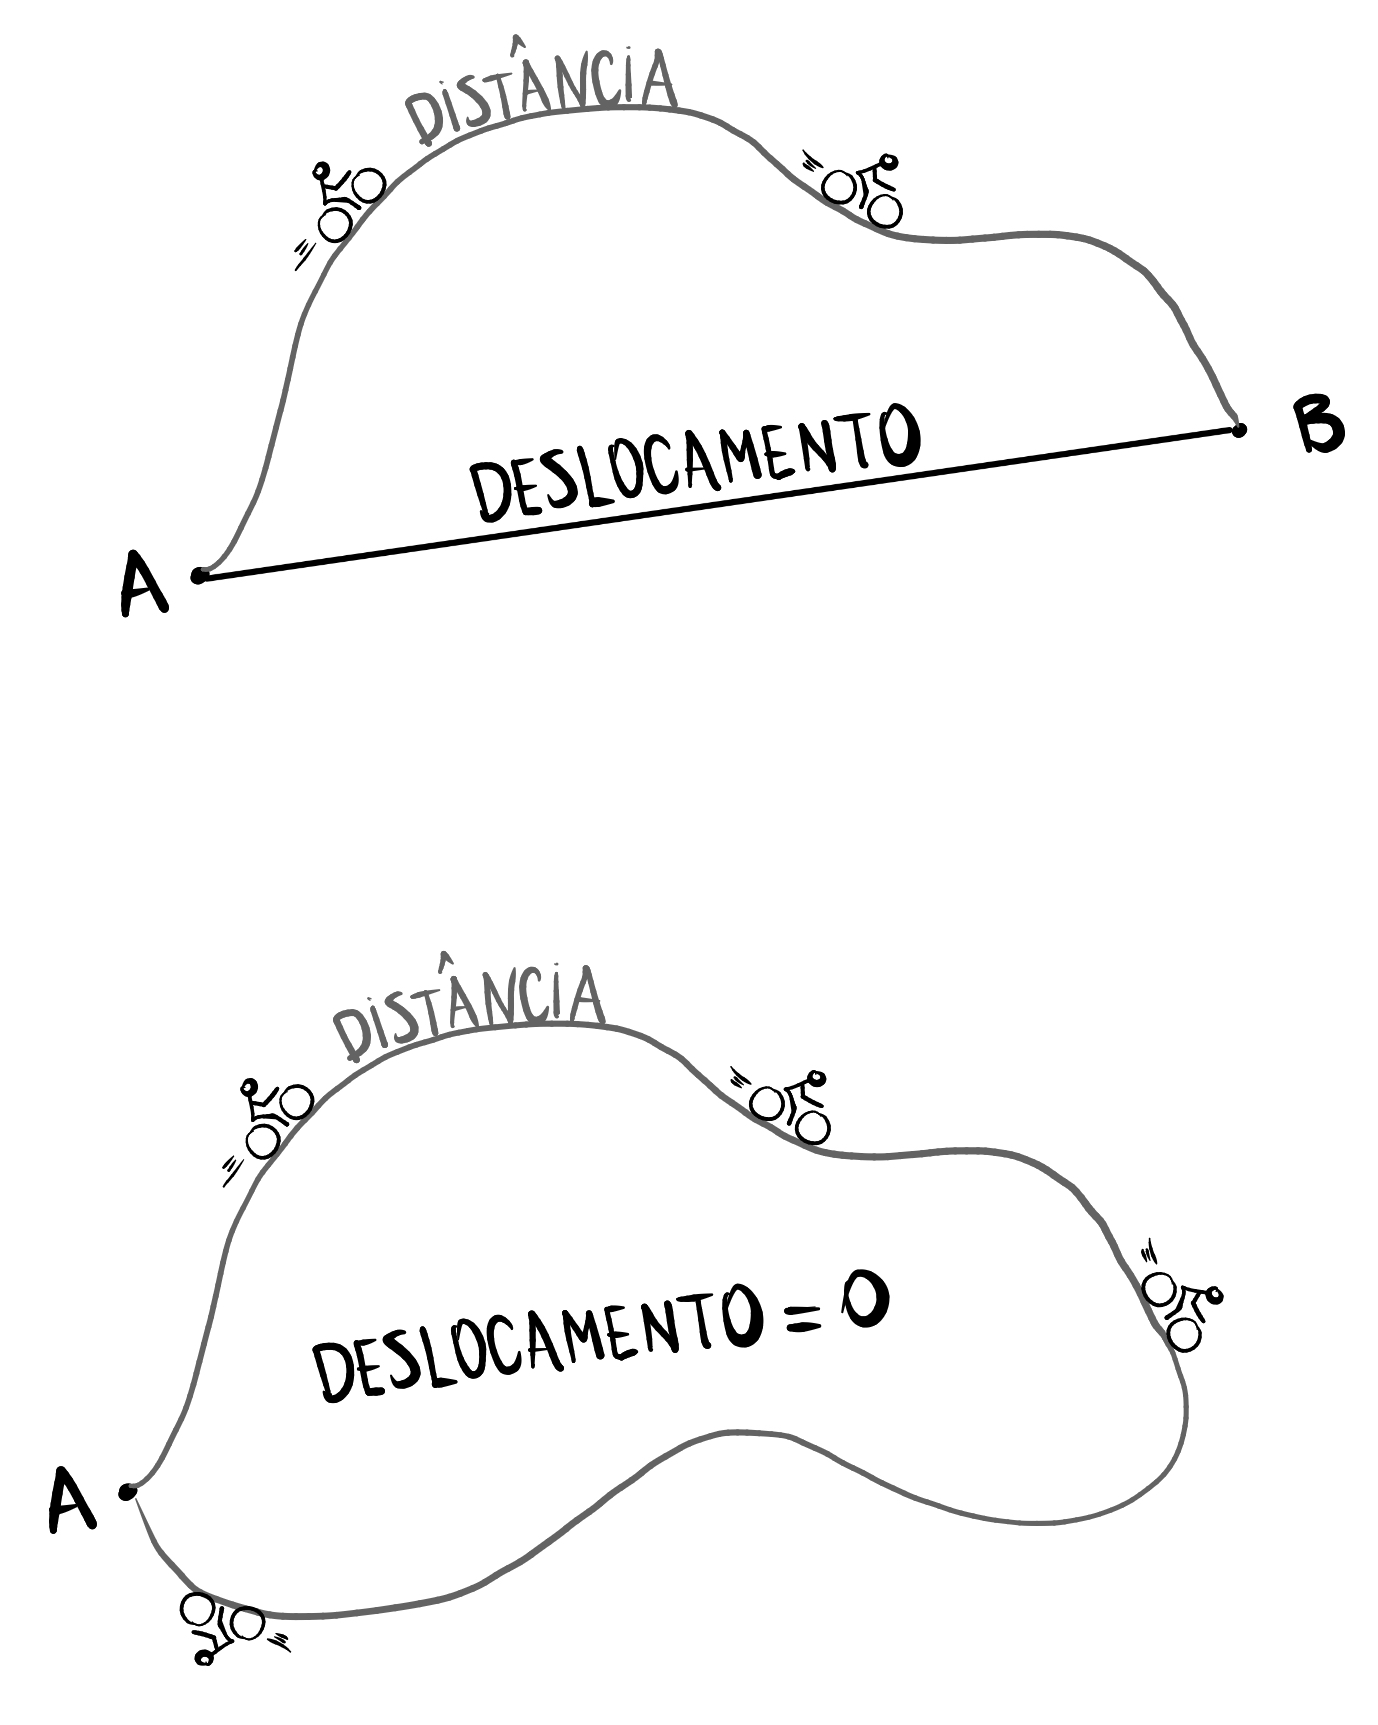
\includegraphics[scale=0.18]{imagensmecanica/deslocamentovsdistancia02.jpeg}
%     \caption{A diferença entre o deslocamento $\Delta s$ e a distância percorrida $d$.}
%     \label{fig_mec_deslocamento_vs_distancia02}
% \end{figure}



Como dito, em vários contextos a distância e o deslocamento irão coincidir. A Figura \ref{fig_mec_deslocamento_vs_distancia02} serve para mostrar um contexto em que isso não ocorre, a fim de deixar clara a diferença entre as duas grandezas.

Agora, a essa altura, o leitor poderia indagar:

\begin{center}
\textit{Ok, até entendi a diferença entre os dois...mas por que a velocidade é definida com base no deslocamento e não na distância?}
\end{center}

Essa, caro leitor, seria uma pergunta deveras inteligente...mas, infelizmente, não temos ferramentas, a essa altura, para respondê-la, de modo que a discussão terá que ficar para um momento futuro.\footnote{Nós poderíamos, inclusive, definir duas grandezas diferentes -- o que de fato ocorre, pelo menos em língua inglesa. Em português não se costuma encontrar isso na literatura, mas em literaturas em língua inglesa é comum que se defina o termo \textit{speed}, ou seja, a rapidez do movimento, como sendo a razão da distância dividida pelo intervalo de tempo. Já o termo \textit{velocity} seria a própria velocidade, que é a razão entre o deslocamento pelo tempo. Como podemos criar conceitos a nosso bel prazer, é possível que tenhamos esses dois conceitos diferentes para medir o movimento: a \textbf{rapidez}, que mede o ``movimento total'', e a \textbf{velocidade}, que mede o ``movimento líquido''. A razão da velocidade, ou seja, de se medir o movimento por meio do deslocamento, ser mais relevante e útil do que a medida do movimento a partir da distância -- o conceito de \textit{speed} -- é o que ficará claro mais adiante.}


Para concluir: na Física, velocidade média não é uma medida de quão longo foi o caminho percorrido, mas de quão diferente é a posição final da posição inicial. Por isso, ela é definida a partir do deslocamento, e não da distância.


\secgfe{Onde é usada}

Como a Cinemática se propõe a estudar o movimento dos corpos, e a velocidade é a grandeza fundamental que mede o movimento, ela aparecerá em absolutamente todas as equações da Cinemática. Além disso, em todas as equações que envolvem o movimento, a velocidade também estará lá. Como um exemplo disso, temos a energia cinética, que é a energia associada ao movimento. Naturalmente, a velocidade irá aparecer em tal equação. Já a força magnética $F_M$ em uma carga elétrica depende do movimento da partícula ao longo do campo, de modo que a velocidade $v$ também irá aparecer em tal equação.

\[
\underbrace{E_c = \frac{1}{2}mv^2}_{\text{Energia cinética}} \quad ; \quad
\underbrace{v^2 = v_0^2 + 2a\Delta s}_{\text{Equação de Torricelli}} \quad ; \quad 
\underbrace{F_M = Bqv\sin\theta}_{\text{Força magnética}} \quad ; \quad
\]


\secgfe{Erros comuns}


\begin{itemize}
    \item [(i)] Considere a Figura \ref{fig_mec_deslocamento_vs_distancia}, que mostra um objeto que sai da posição $s_0=3$ m, se desloca 10m para a direita, e depois retorna 10m para esquerda, terminando na posição $s_f=3$m. Digamos que tal movimento ocorre ao longo de um intervalo de tempo de $5$s. Ora, intuitivamente o leitor poderia pensar:
    
    \textit{Se o objeto percorre uma distância de 20m (10m na ida e 10m na volta) durante 5s, então sua velocidade é $v=\sfrac{d}{t} = \sfrac{20\text{m}}{5\text{s}} = 4$ m/s.} 


    \begin{figure}[h]
    \centering
    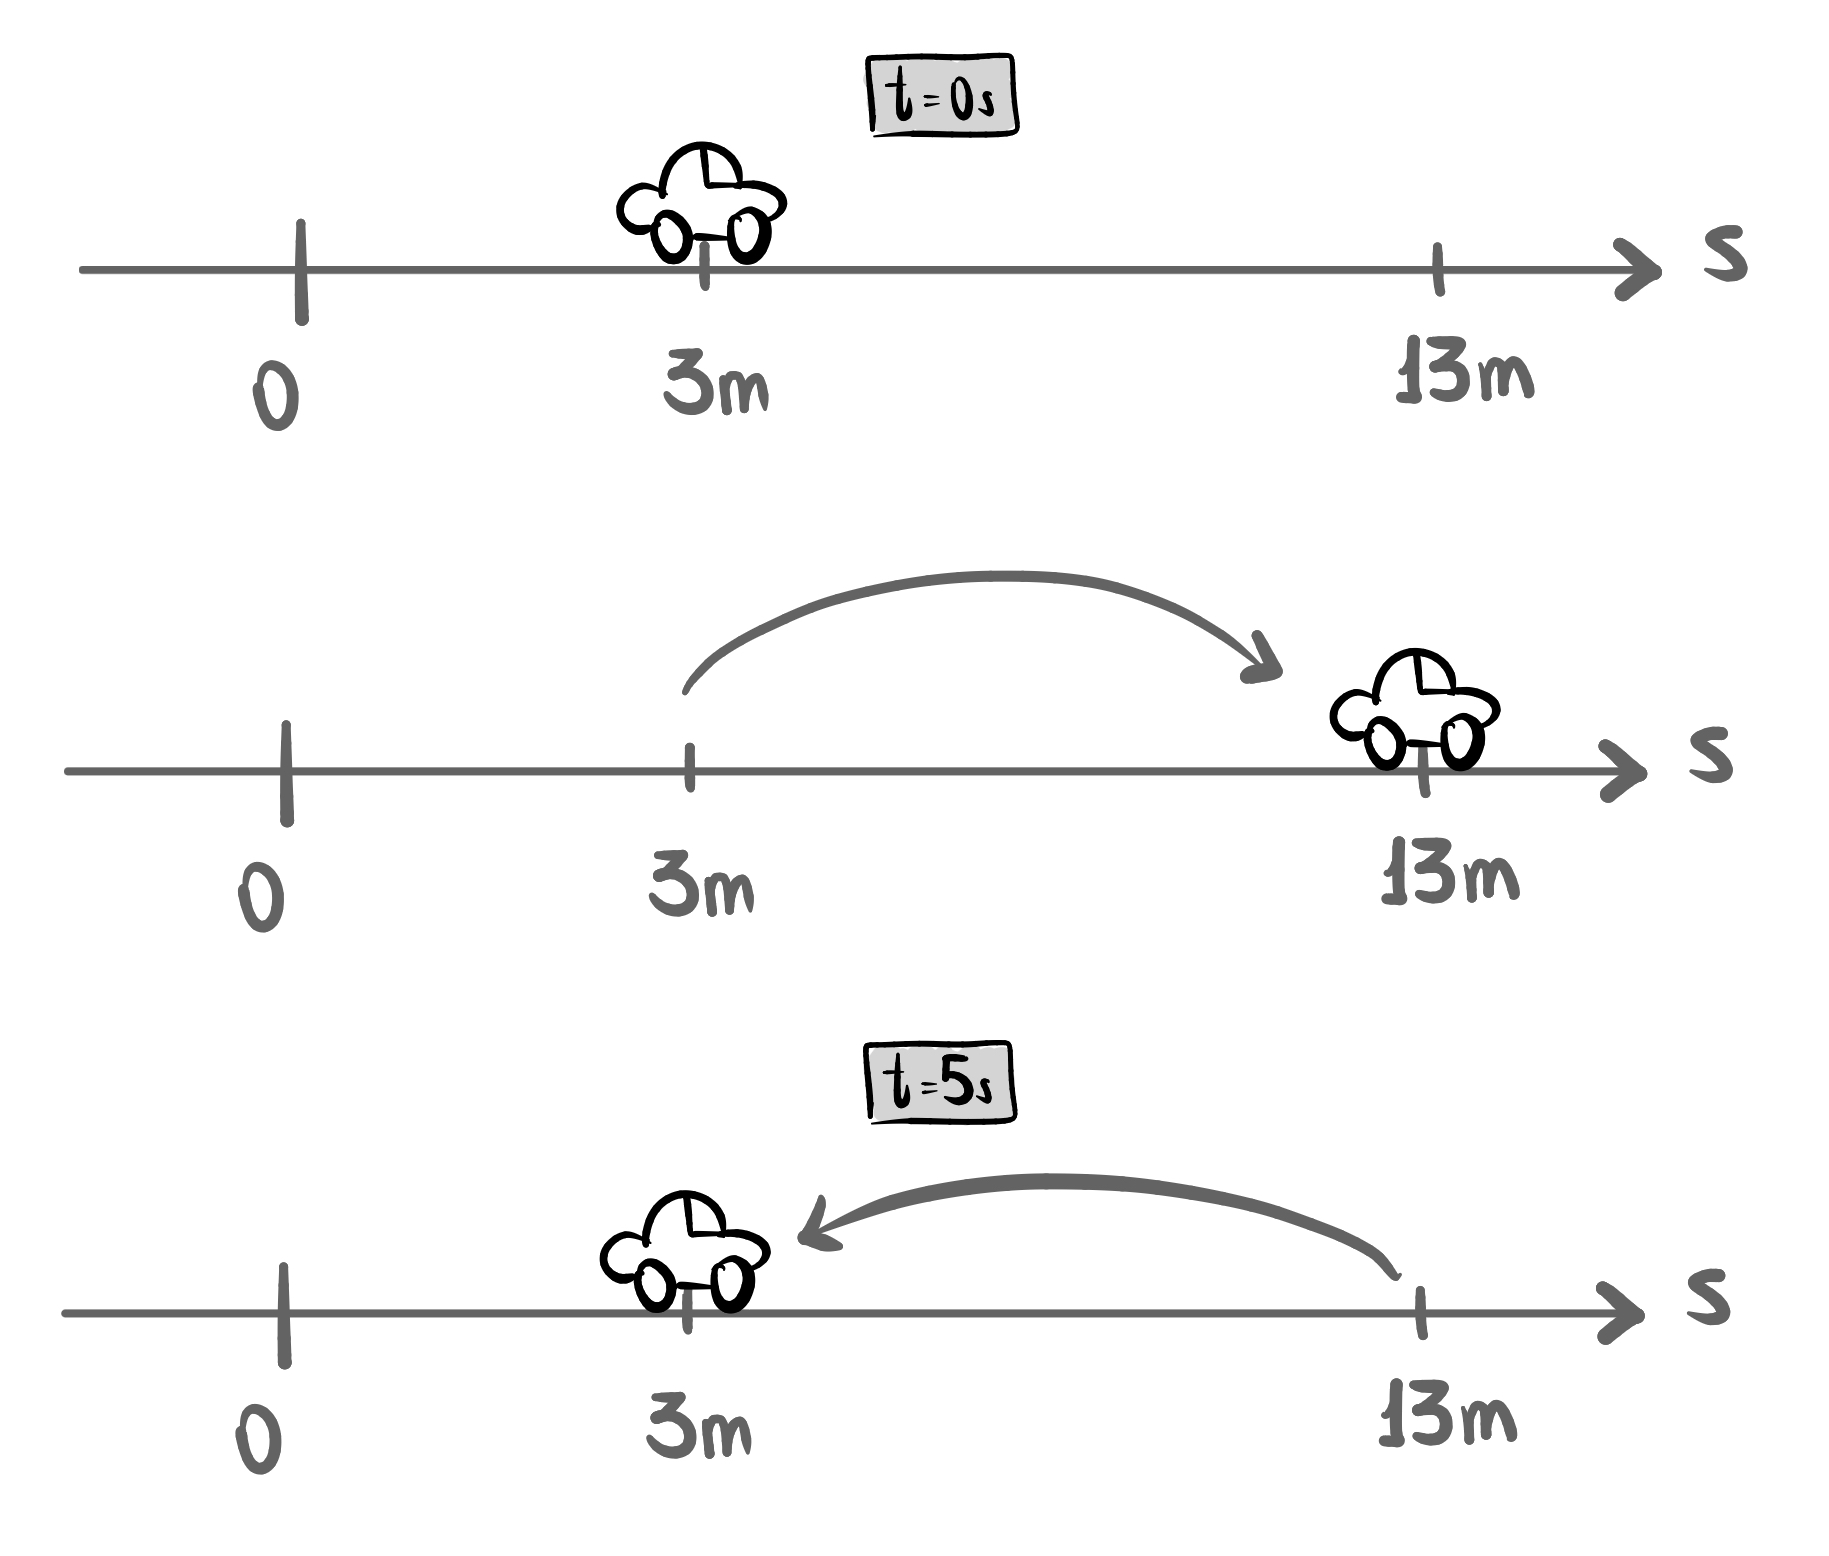
\includegraphics[scale=0.15]{imagensmecanica/deslocamentovsdistanciaescalar.jpeg}
    \caption{A distância percorrida é de 20m, mas o deslocamento, isto é, o quanto o corpo se afastou da sua posição inicial, é nulo.}
    \label{fig_mec_deslocamento_vs_distancia}
\end{figure}

    
    Isso, contudo, estaria errado, segundo a definição feita na Equação \eqref{mecanica_eq_velocidademedia}. A velocidade média neste trecho seria, na verdade, dada por

    $$ v_m = \dfrac{\Delta s}{\Delta t} = \dfrac{s_f-s_0}{t_f-t_0} = \dfrac{3-3}{5 \text{ s}} = 0 \text{ m/s}. $$

    Por mais estranho que isso possa lhe parecer, essa é a definição que fizemos: queremos medir o quanto o objeto se afastou da sua posição inicial e, se ele começa em uma posição e termina na mesma posição, ele não se afastou -- no resultado final de seu movimento -- do seu ponto de partida, de modo que seu deslocamento -- a variação $\Delta s$ da posição -- é nulo, o que resulta em uma velocidade média nula neste trecho, por mais que o objeto tenha se movido ao longo do tempo.

    O erro aqui, portanto, é considerar a distância, e não o deslocamento escalar, para o cálculo da velocidade média.

    \item [(ii)] Considere um carro que sai da cidade A, avança 120 km em 2 horas, e para a fim de abastecer em um posto. O motorista, além de abastecer, resolve fazer um lanche, ficando parado por 1 hora. Em seguida, ele sai do posto, se deslocando por mais 180 km, na mesma direção e sentido, para a cidade B. Se este último trecho é feito em outras 2 horas, qual foi a sua velocidade média ao longo da viagem?


    Existem vários erros diferentes que podem ser cometidos aqui, vamos tentar passar pelos mais comuns.

    \begin{enumerate}
        \item O estudante faz a velocidade média em cada trecho do movimento, e depois faz a média entre elas. Ou seja, no primeiro trecho, da cidade A ao posto, a velocidade média foi de 120km/2h = 60 km/h. No segundo trecho, do posto à cidade B, a velocidade média foi de 180km/2h = 90 km/h. Fazendo a média, teremos
        $$ v_m = \dfrac{60+90}{2} = 75 \text{ km/h.}$$

        Este resultado -- e tal raciocínio -- está totalmente errado. O erro aqui é confundir velocidade média, que é uma grandeza física cujo significado é definido e encapsulado pela Equação \eqref{mecanica_eq_velocidademedia}, com a média aritmética das velocidades. Talvez a confusão seja por tal grandeza levar o termo \textit{média} no nome, mas isso de fato não tem absolutamente nenhuma relação com o cálculo da média aritmética entre números. Tal raciocínio não faz nenhum sentido, haja vista que, pela forma como definimos a velocidade média, o conceito de média aritmética não tem nenhuma relação com a forma como se calcula tal grandeza.

        \item O estudante desconsidera o tempo em repouso, considerando que o carro teve um deslocamento total de $120+180 = 300 $ km, ao longo de um tempo total de movimento de $2+2 = $ 4h, o que daria uma velocidade média, pela definição, de 

        $$ v_m = \dfrac{\Delta s}{\Delta t} = \dfrac{300 \text{ km}}{4 \text{ h}} = 75 \text{ km/h}.$$

        Neste caso, o estudante aplicou a definição corretamente, porém errou na hora mensurar uma das grandezas envolvidas em tal definição. O deslocamento total está correto, é de fato de 300 km. Porém o intervalo de tempo que entra ali é o tempo total de movimento -- desde o carro sair da cidade A até chegar na cidade B, não importando se ele fez pausas no meio do caminho. Por termos desconsiderado o tempo em repouso, chegamos no resultado errado.\footnote{Note que, com este erro, chegamos no mesmo resultado numérico do erro anterior, de 75 km/h. O que foi uma coincidência -- um erro poderia ter nos levado a um valor de velocidade de 75 km/h, enquanto o outro tipo de erro poderia ter nos levado a um valor de 50 km/h, ou qualquer outro. Não se apegue a tal coincidência.}
    \end{enumerate}

O cálculo correto da velocidade média, neste caso, considera o deslocamento total de $120+180 = 300 $ km, ao longo de um intervalo de tempo de $2+2+1 = $ 5h, que é o tempo total de viagem. Isso dá uma velocidade média, pela definição, de 

        $$ v_m = \dfrac{\Delta s}{\Delta t} = \dfrac{300 \text{ km}}{5 \text{ h}} = 60 \text{ km/h}.$$


        O significado disso é o que se segue: um carro que tivesse saído do mesmo local, e se movido durante o mesmo intervalo de tempo total de viagem (5 horas, no caso), com uma velocidade constante de $60$ km/h, teria, ao final das 5 horas, percorrido a mesma distância total.
    
    
\end{itemize}






\secgfe{Observações}


No Sistema Internacional de Unidades de Medida (SI) a unidade padrão para medir distância é metro (m) e a unidade padrão para medir tempo é o segundo (s), de modo que a unidade de medida para velocidade no SI é dada em m/s.

É claro que alguém poderia medir a velocidade em $\text{km}/\text{s}$ ou  $\text{m}/\text{h},$ ou quaisquer outras unidades em que se tem uma unidade de distância no numerador e uma unidade de tempo no denominador. Fora do SI, a unidade mais comum para se medir velocidade é em km/h, de modo que é interessante conhecer a conversão entre tal unidade e aquela do SI, que é dada pela transformação:

\begin{equation}
    \boxed{1 \dfrac{ \text{m}}{\text{s}} = 3,6 \dfrac{\text{km}}{\text{h}}.}
      \label{mecanica_eq_convertermsparakmh}
\end{equation}

Ou seja, em palavras, se você anda 1 metro a cada segundo, você irá percorrer uma distância de 3,6 km ao longo de uma hora. Uma forma intuitiva de lembrar disso é a seguinte: via de regra, uma passada humana varre uma distância de 1 metro. É claro que isso vai variar um pouco para pessoas de diferentes alturas, haja vista que o tamanho da sua perna é o que irá definir o avanço ao longo de uma passada -- mas tal valor, de um metro, é razoável para ser considerado como uma boa média. Dito isso, se você estiver fazendo uma caminhada em ritmo leve, é comum você dar um passo a cada segundo (faça o teste), o que significa que, em tal caminhada -- na qual você avança 1 metro a cada 1 segundo -- você irá percorrer uma distância de 3,6 km se permanecer caminhando ao longo de 1 hora. 

Convido o leitor a fazer o teste e verificar, por si mesmo, que caminhando por 1 hora você avançará uma distância bem próxima de 3,6 km (como dito, o comprimento de suas pernas pode fazer essa distância variar um pouco para cima ou para baixo).

Agora que o leitor possui uma forma empírica de verificar a Equação \eqref{mecanica_eq_convertermsparakmh}, vamos à sua verificação matemática:

$$ 1 \dfrac{\text{km}}{\text{h}} = \dfrac{1000 \text{ m}}{3600 \text{ s}} = \dfrac{1}{3,6} \dfrac{\text{m}}{\text{s}} \implies 1 \dfrac{ \text{m}}{\text{s}} = 3,6 \dfrac{\text{km}}{\text{h}}. $$

Note que usamos que 1 hora possui 3600 segundos (60 minutos, com 60 segundos em cada: $60\cdot 60 = 3600 )$ e que 1 km são 1000 m. O resto são apenas manipulações algébricas.



\vspace{0.3cm}

\begin{exemplo}[Nível I]\label{exemplo_cinematicaescalar_velocidademedia01}

Converta as velocidades abaixo entre m/s e km/h:

\begin{enumerate}
    \item [(a)] 10 m/s
    \item [(b)] 20 m/s
    \item [(c)] 30 m/s
    \item [(d)] 90 km/h
    \item [(e)] 135 km/h
\end{enumerate}


\resolucao


A regra prática que se extrai da Equação \eqref{mecanica_eq_convertermsparakmh} é: se a velocidade está em m/s, multiplica-se tal valor por 3,6 para obtê-la em km/h. Se ela está em km/h, divide-se tal valor por 3,6 para obtê-la em m/s. Faremos isso, como se segue:

\begin{enumerate}
    \item  [(a)] 10 m/s \quad $\xrightarrow{\text{multiplicando por 3,6}} \quad 36 \text{ km/h}.$
    \item  [(b)] 20 m/s \quad $\xrightarrow{\text{multiplicando por 3,6}} \quad 72 \text{ km/h}.$
    \item  [(c)] 30 m/s \quad $\xrightarrow{\text{multiplicando por 3,6}} \quad 108 \text{ km/h}.$
    \item  [(d)] 90 km/h \quad $\xrightarrow{\text{dividindo por 3,6}} \quad 25 \text{ m/s}.$
    \item  [(e)] 135 km/h \quad $\xrightarrow{\text{dividindo por 3,6}} \quad 37,5 \text{ m/s}.$
\end{enumerate}

    
\end{exemplo}





\vspace{0.3cm}

\begin{exemplo}[Nível II (AFA - 2011)]\label{exemplo_cinematicaescalar_velocidademedia02}

Um turista, passeando de bugre pelas areias de uma praia em Natal--RN, percorre uma trajetória triangular, que pode ser dividida em três trechos, conforme a figura abaixo.

{
\centering
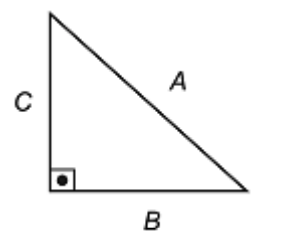
\includegraphics[width=0.2\linewidth]{imagensmecanica/exemplovmedianivel2afa.png}
\captionof{figure}{}
\label{fig_mec_exemplovelocidademedianivel2AFA}
} 


Os trechos $B$ e $C$ possuem o mesmo comprimento, mas as velocidades médias desenvolvidas nos trechos $A$, $B$ e $C$ foram, respectivamente, $v$, $2v$ e $v$. A velocidade escalar média desenvolvida pelo turista para percorrer toda a trajetória triangular vale

\begin{enumerate}
  \item [(a)] $v\sqrt{2}$
  \item [(b)] $2v\sqrt{2}$
  \item [(c)] $4v$
  \item [(d)] $(4 - 2\sqrt{2})\,v$
\end{enumerate}

\resolucao

Seja $x$ o comprimento dos trechos $B$ e $C$, logo, o trecho $A$ possui comprimento $x\sqrt 2.$ Essa é uma boa questão para que o aluno fique atento aos termos. Note que, a rigor, a velocidade escalar média seria nula, haja vista que o deslocamento total foi nulo -- o turista retorna ao mesmo ponto de partida. Contudo, nota-se que não há essa opção nas alternativas, de modo que o estudante atento já deve se dar conta de que houve um deslize conceitual por parte da banca que enunciou a questão. Sendo assim, é fácil induzir que estão tratando da \textit{rapidez} com que o turista se moveu, isto é, a razão entre a distância total percorrida por ele no tempo. \\

Logo, sendo $\Delta t_A$, $\Delta t_B$ e $\Delta t_C$ os tempos necessários para percorrer os trechos $A,$ $B$ e $C,$ respectivamente, teremos que a velocidade média em todo o trecho será

$$ v_m = \dfrac{d_A+d_B+d_C}{\Delta t_A+\Delta t_B+\Delta t_C}=\dfrac{x\sqrt 2+x+x}{\Delta t_A+\Delta t_B+\Delta t_C} = \dfrac{x(2+\sqrt 2)}{\Delta t_A+\Delta t_B+\Delta t_C} .$$

Resta-nos, portanto, obter os tempos de cada trecho:

$$ \Delta t_A=\dfrac{x\sqrt 2}{v}; \quad \Delta t_B=\dfrac{x}{2v}; \quad \Delta t_C=\dfrac{x}{v},$$

\noindent de modo que o tempo total é 

$$\Delta t_A+\Delta t_B+\Delta t_C =  \dfrac{2x\sqrt 2+x+2x}{2v} = \dfrac{x(2\sqrt 2+3)}{2v}, $$

\noindent e, portanto, a velocidade média em todo o trecho foi


$$v_m =\dfrac{x(2+\sqrt2)}{\Delta t_A+\Delta t_B+\Delta t_C} = \cancel{x}(2+\sqrt2) \cdot \dfrac{2v}{\cancel{x}(2\sqrt2+3)} =2v\dfrac{(2+\sqrt2)}{(2\sqrt2+3)},$$

\noindent e, multiplicando por $(3-2\sqrt2)$ o numerador e o denominador para racionalizar, chegamos em

$$  \boxed{ v_m=v(4-2\sqrt2) \implies \text{Letra D.}}$$


    
\end{exemplo}


\vspace{0.3cm}




\begin{exemplo}[Nível III]\label{exemplo_cinematicaescalar_velocidademedia03}

Um móvel desloca-se ao longo de uma trajetória retilínea de comprimento total $L$, dividida em infinitos trechos consecutivos. Em cada trecho o móvel sempre percorre metade da distância restante. Compute a velocidade média do móvel em todo o percurso nos casos em que


\begin{itemize}
  \item [(a)] a velocidade $v$ com que o móvel percorre cada trecho é sempre a mesma.
  
  \item [(b)] a velocidade $v$ com que o móvel percorre cada trecho é sempre a igual à metade da velocidade usada no trecho imediatamente anterior.

  \item [(c)] a velocidade $v$ com que o móvel percorre cada trecho é sempre a igual ao dobro da velocidade usada no trecho imediatamente anterior.
  
\end{itemize}



\resolucao



Nos três casos, note que, ao longo do movimento completo, o deslocamento total (que neste caso coincide com a distância percorrida) do corpo é igual a $L$. Logo, sendo $\Delta t$ o seu tempo total de movimento, teremos que a velocidade média $v_m$ ao longo de todo o movimento será

\begin{equation}
    v_m = \dfrac{\Delta s}{\Delta t} = \dfrac{L}{\Delta t}.
    \label{mecanica_eq_velocidademediaexemplonivelIII}
\end{equation}



O movimento, contudo, é quebrado em infinitas etapas, as quais serão usadas para computar o tempo de cada trecho. Ou seja, o tempo total de movimento $\Delta t$ será quebrado em infinitas partes, cada uma para uma etapa do deslocamento:

$$ \Delta t= \Delta t_1+\Delta t_2+\Delta t_3 + \dots,$$

\noindent em que $\Delta t_i$ representa o intervalo de tempo necessário para o móvel percorrer o $i$-ésimo trecho. Avaliemos cada caso, agora, individualmente.


\begin{itemize}
  \item [(a)] Neste caso a velocidade é sempre $v$, de modo que o tempo de percurso de cada etapa é:

    \begin{enumerate}
        \item [(i)] No primeiro trecho ainda resta a distância total $L$ a ser percorrida, de modo que aqui percorreremos metade deste trecho, o que leva um tempo 

        $$ \Delta t_1 = \dfrac{L/2}{v} = \dfrac{L}{2v}.$$


        \item [(ii)] Agora, no segundo trecho, resta a distância total $L/2$ a ser percorrida, de modo que aqui percorreremos metade deste trecho, o que leva um tempo

        $$ \Delta t_2 = \dfrac{L/4}{v} = \dfrac{L}{4v}.$$


        \item[(iii)]  Resta agora a distância total $L/4$ a ser percorrida, de modo que aqui percorreremos metade deste trecho, o que leva um tempo

        $$ \Delta t_3 = \dfrac{L/8}{v} = \dfrac{L}{8v}.$$
    \end{enumerate}

Já está claro qual é o padrão, de modo que o tempo total de movimento é 
$$\Delta t_A = \dfrac{L}{2v}+\dfrac{L}{4v}+\dfrac{L}{8v}+\dfrac{L}{16v}+\dots  = \dfrac{L}{2v} \left( 1+\dfrac{1}{2} + \dfrac{1}{4} + \dfrac{1}{8}+\dots \right),$$

\noindent em que a soma se estende até o infinito. Note que tal soma é uma progressão geométrica, de termo inicial $a_1=1$ e razão $q=\sfrac{1}{2},$ cuja soma é 

 $$ 1+\dfrac{1}{2} + \dfrac{1}{4} + \dfrac{1}{8}+\dots = \dfrac{a_1}{1-q} = \dfrac{1}{1-\sfrac{1}{2}} = 2,$$

 \noindent logo, o tempo total neste caso é 

 $$ \Delta t_A = \dfrac{L}{2v}\cdot 2 \implies \Delta t_A = \dfrac{L}{v}.$$

 Assim, pela Equação \eqref{mecanica_eq_velocidademediaexemplonivelIII}, a velocidade média neste trecho será

 $$ \boxed{ v_A = \dfrac{L}{\Delta t_A} = \dfrac{L}{L/v} = v}.$$

 Pensando bem, o leitor verá que tal resposta é óbvia: se vamos percorrer o movimento inteiro com a mesma velocidade constante $v$, não importa em quantos trechos o movimento será subdividido -- sendo a velocidade sempre igual a $v$, em qualquer trecho avaliado (seja em apenas um pedaço ou no trecho completo do movimento) a velocidade média será sempre igual a $v.$ \\
 
 Este é um problema baseado no famoso paradoxo de Zenão de Eleia, sobre Aquiles e a Tartaruga. A ideia é que, se dividirmos um movimento finito, como o percurso de uma distância $L$, em infinitas etapas, somos levados a crer que a tarefa nunca será concluída. Contudo, isso é uma inverdade -- é possível varrer infinitas etapas de um processo em um tempo finito, como é o caso aqui, haja vista que a soma dos infinitos tempos é conhecida -- a soma dos infinitos termos de uma P.G. -- e é finita, neste caso. \\

 Desse modo, não era exatamente necessário ter feito todos os cálculos aqui -- de fato era imediato a resposta de que a velocidade média seria $v.$ Contudo, tal desenvolvimento será importante para os próximos itens.
  
  \item [(b)] Note que, neste caso, a velocidade não é constante -- ela assume valores diferentes em cada trecho, de modo que o raciocínio não será tão simples como o anterior. Aqui teremos de fato que avaliar o que ocorre em cada trecho do movimento. Avaliemos cada trecho e o respectivo tempo que leva para percorrê-lo:

   \begin{enumerate}
    \item [(i)] Inicialmente resta a distância total $L$ a ser percorrida, de modo que aqui percorreremos metade deste trecho, com velocidade $v$, o que leva um tempo

    $$ \Delta t_1 = \dfrac{L/2}{v} = \dfrac{L}{2v}.$$


\item [(ii)] Resta-nos agora varrer a distância $L/2$ para concluir o movimento. Neste trecho, percorrer-se-á metade de tal distância, com metade da velocidade anterior, isto é, $v/2,$ o que leva um tempo:

$$ \Delta t_2 = \dfrac{L/4}{v/2} = \dfrac{L}{2v}.$$


\item [(iii)] Resta-nos agora varrer a distância $L/4$ para concluir o movimento. Neste trecho, percorrer-se-á metade de tal distância, ou seja, $L/8$, com metade da velocidade anterior, isto é, $v/4,$ o que leva um tempo:

$$ \Delta t_3 = \dfrac{L/8}{v/4} = \dfrac{L}{2v}.$$

    
\end{enumerate}


A essa altura o leitor já percebeu que o formato para se calcular o intervalo de tempo de duração do $i$-ésimo trecho é do tipo

$$ \Delta t_i = \dfrac{L/2^n}{v/2^{n-1}},$$

\noindent o que sempre resulta em $L/(2v),$ qualquer que seja o valor de $n \geq 1.$


Logo, o tempo total de movimento seria

$$ \Delta t_B =  \Delta t_1+\Delta t_2+\Delta t_3 + \dots= \dfrac{L}{2v}(1+1+1+1+\dots)= \infty,$$

\noindent de onde concluiríamos que a velocidade média, dada por $v_C = L/\Delta t$, tende a zero. O que aconteceu aqui? \\

Talvez o leitor tenha estranhado, mas está tudo normal. É impossível percorrer o trecho de comprimento $L$ da forma como proposto, por isso chegamos em tal resposta: a nossa partícula, na verdade, nunca termina de percorrer o comprimento $L$ inteiro.

Isso acontece porque, em cada novo trecho, apesar de termos que percorrer metade da distância, faremos isso com metade da velocidade, de modo que levaremos o mesmo tempo. Assim, é como se eu te dissesse: \textit{vou fazer infinitas caminhadas, cada uma durando 10 minutos. Quanto tempo levo para terminar tal tarefa?}. \\

Ora, são infinitas etapas com um tempo de duração de 10 minutos -- que seria o nosso $L/(2v)$ --, logo, o tempo total é infinito e a tarefa nunca é concluída. É diferente de quando percorremos metade da distância remanescente mantendo a mesma velocidade, pois isso faz com que o tempo para cumprir cada nova etapa seja cada vez menor, o que pode possibilitar que a soma desses infinitos intervalos de tempo seja finita, como foi o caso do item anterior.


  \item [(c)] Neste caso a velocidade também não é constante, assumindo valores diferentes em cada trecho. Vamos tentar construir uma intuição antes de fazer os cálculos. 

  Perceba que, a cada novo trecho, a distância percorrida diminui -- é sempre metade da distância anterior --, porém agora a velocidade com que se percorre essa distância aumenta -- é sempre o dobro da velocidade do trecho anterior. Assim, o tempo necessário para percorrer cada trecho vai ficando cada vez menor: percorreremos distâncias cada vez menores com velocidades cada vez maiores. Isso deve nos levar a crer que, diferente do item anterior, a soma dos infinitos intervalos de tempo de cada trecho, aqui, deve ser finita, uma vez que os intervalos de tempo ficam cada vez menores. \\

  Indo além, seria razoável esperar, inclusive, que o tempo total neste caso seja menor do que o tempo necessário para varrer a distância $L$ no item $(a),$ uma vez que lá as etapas são feitas sempre com a mesma velocidade $v$, enquanto aqui as novas etapas são feitas com velocidades cada vez maiores, resultando em intervalos de tempo que vão ficando ainda mais curtos do que aqueles que apareciam no caso do item $(a).$ \\

  O leitor pode verificar, neste caso, que a solução será bem semelhante ao do item $(a),$ resultando em um progressão geométrica análoga, porém com razão $q=\sfrac{1}{4}$ -- a distância percorrida em um novo trecho cai pela metade, porém a velocidade com que ele é percorrido dobra, por isso o fator $\sfrac{1}{2^2}$ aparece aqui, e apenas $\sfrac{1}{2}$ no item $(a)$. Assim, o tempo total de movimento é

  $$ \Delta t = \dfrac{L}{2v} \left(1+\dfrac{1}{4}+\dfrac{1}{16}+\dots \right) = \dfrac{L}{2v} \left( \dfrac{a_1}{1-q} \right) = \dfrac{L}{2v}\left( \dfrac{1}{1-\sfrac{1}{4}} \right) =  \dfrac{2L}{3v},$$

\noindent o que resulta, pela Equação \eqref{mecanica_eq_velocidademediaexemplonivelIII}, em uma velocidade média

$$ \boxed{ v_C = \dfrac{L}{\Delta t_C} = \dfrac{L}{\sfrac{2L}{3v}} = \dfrac{3v}{2}.}$$

Para chegar nessa resposta o leitor poderia ter tomado um caminho diferente e raciocinar apenas por comparação com o item $(a):$ no contexto do item $(c)$, em cada trecho, o tempo para percorrê-lo será exatamente metade do tempo para percorrer o mesmo trecho no contexto do item $(a);$ logo, o tempo total de movimento aqui será metade daquele, fazendo com que a velocidade média aqui -- uma vez que a distância total é a mesma -- seja o dobro daquela. Logo, concluiríamos que $v_C = 2v,$ e erraríamos em 33\% a resposta, haja vista que o valor correto é $v_C=1.5v$ \\

O leitor consegue perceber qual é o erro em tal raciocínio? \footnote{Vou dar uma dica para que o leitor possa refletir. Contudo, é importante que as palavras que se seguem sejam lidas apenas após o estudante colocar uma energia mínima em tentar descobrir por si só. Note que existe um único trecho -- o primeiro -- em que o raciocínio aplicado não caberia. No primeiro trecho do movimento -- o percurso de $L/2$, metade da distância total -- os tempos de percurso nos itens $(a)$ e $(c)$ são os mesmos. E por que será que uma diferença de apenas um trecho, entre infinitos, é capaz de gerar uma resposta que diverge em 33\% da resposta correta...?}
  
\end{itemize}





\end{exemplo}

\vspace{0.3cm}







\begin{secnivel}[Velocidade Relativa]{I}{Velocidade Relativa}
  
  \eqLdois{def}{mecanica_eq_velocidaderelativa}{v_{AB} = v_A \pm v_B}

\end{secnivel}








\secgfe{De onde vem}
 
A Equação \eqref{mecanica_eq_velocidaderelativa} nos permite obter a velocidade relativa $v_{AB}$ do objeto $A$ em relação ao objeto $B$. Mas o que raios seria uma velocidade relativa?

Giordano Bruno, contemporâneo de Galileu e coaduno de suas ideias a respeito da astronomia, escreveu, em sua obra \textit{De l’infinito, universo e mondi} de 1584 que

\begin{quote}
    “Nada está absolutamente imóvel; o movimento e o repouso existem apenas por comparação.”
\end{quote}


Essa ideia contém, com profundidade, um dos princípios mais importantes da teoria do movimento galileana: a ideia de que todo movimento é relativo. Para compreender melhor tal conceito, considere a Figura \ref{fig_mec_galileurepousoemovimento01}, que mostra dois indivíduos, Aristóteles, representado pela letra $A$, e Bohr, representado pela letra $B.$ O tempo passa e, aparentemente, nada acontece: a distância entre Aristóteles e Bohr não se altera, de modo que parece razoável que qualquer um conclua que os dois indivíduos estão em repouso.

Contudo, a Figura \ref{fig_mec_galileurepousoemovimento01} não contém toda a realidade do movimento: Aristóteles e Bohr estão, na verdade, no salão de um grande navio, que está viajando pelo oceano pacífico.

{
\centering
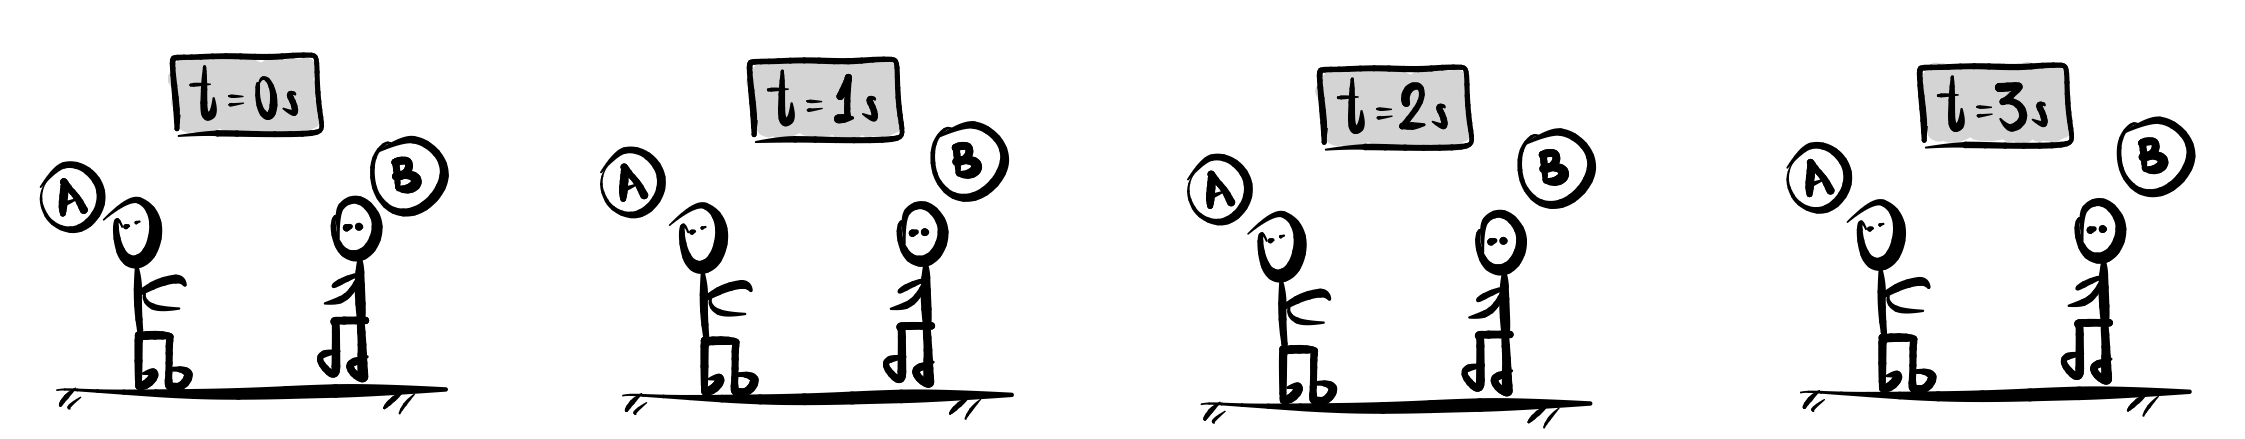
\includegraphics[width=0.9\linewidth]{imagensmecanica/galileu_movimentoerepouso1.jpeg}
\captionof{figure}{Os indivíduos $A$ e $B$ aparentam estar em repouso. }
\label{fig_mec_galileurepousoemovimento01}
} 

A Figura \ref{fig_mec_galileurepousoemovimento02} mostra, gradativamente, tal situação, à medida que vamos dando um \textit{zoom out} na nossa imagem. Note que, à medida que vamos nos afastando, percebemos um terceiro indivíduo, Copérnico, representado pela letra $C$, que aparece em terra firme, observando o navio se mover. Note que, para Copérnico, os indivíduos $A$ e $B$ não estão em repouso: eles se afastam de Copérnico, com a mesma velocidade na qual o navio se move. 

{
\centering
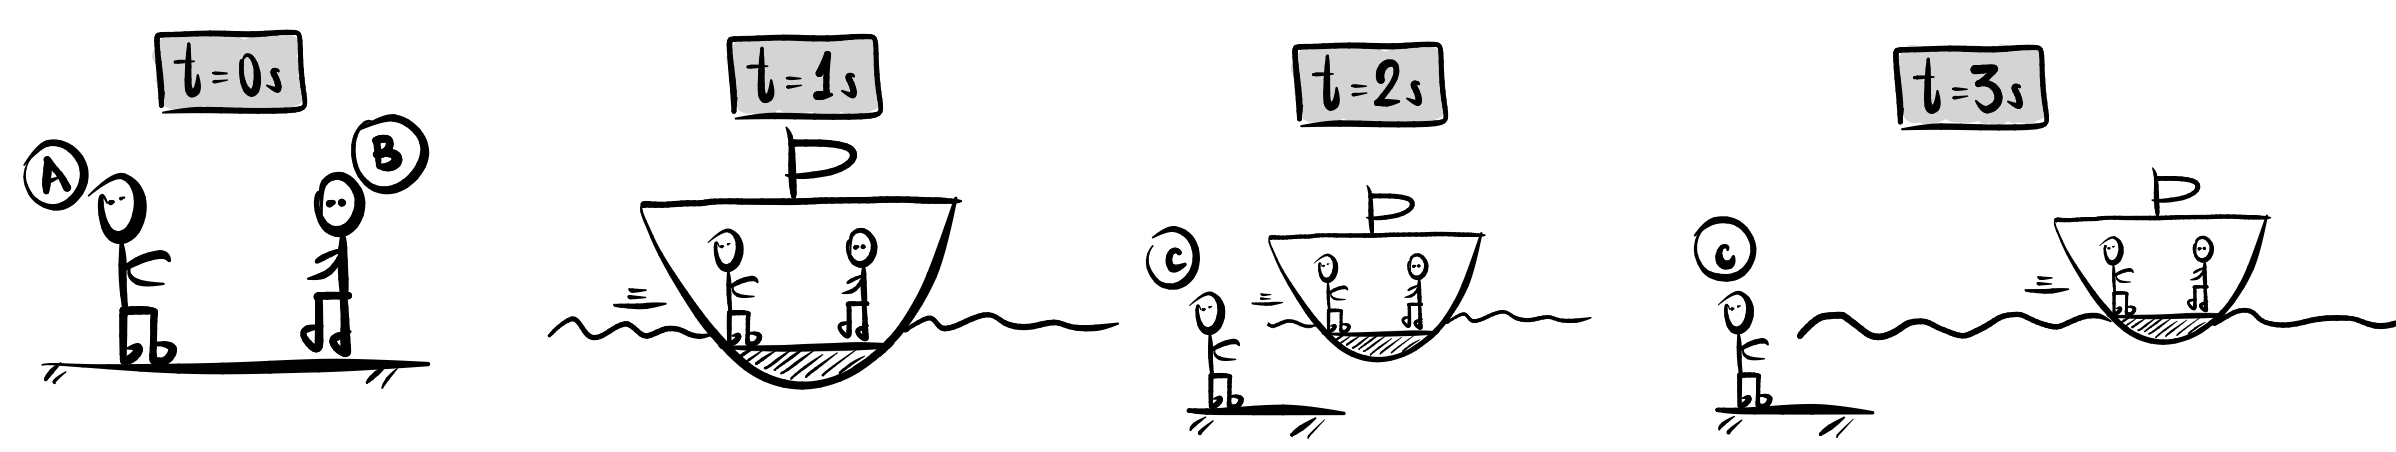
\includegraphics[width=1.0\linewidth]{imagensmecanica/galileu_movimentoerepouso2.jpeg}
\captionof{figure}{Os indivíduos $A$ e $B$ na verdade estão dentro de um navio, que se move em relação ao indivíduo $C.$}
\label{fig_mec_galileurepousoemovimento02}
} 

De modo concreto, caso a velocidade do navio (em relação à terra) seja de $50$ km/h, Copérnico perceberá seus amigos Aristóteles e Bohr se distanciando de si de $50$ km a cada hora que passa. Nesse sentido, seria correto escrever que

$$ v_{AB} = 0,$$

\noindent ou seja, a velocidade de Aristóteles ($A$) em relação à Bohr ($B$) é nula -- um não se move em relação ao outro, o que se evidencia na Figura \ref{fig_mec_galileurepousoemovimento01}. Contudo, não poderíamos dizer que $v_{AC}=0,$ ou seja, como mostra a Figura  \ref{fig_mec_galileurepousoemovimento02}, Aristóteles não está parado em relação à Copérnico, eles se afastam um do outro de 50 km a cada hora, ou seja:

$$ v_{AC}=50 \text{ km/h.}$$



Perceba, portanto, que a pergunta \textit{``qual é a velocidade de Aristóteles?''} não faz sentido. Essa pergunta só faz sentido quando, primeiro, fixarmos um referencial -- em relação a quem tal velocidade é medida. Do contrário, a velocidade Aristóteles pode ser qualquer valor: ela é zero para alguns, $50$ para outros, $120$ para alguns outros, e por aí vai.

É nesse sentido que foi afirmado, no início da seção, que \textbf{toda velocidade é relativa.} Não existe nenhuma grandeza física que se chama ``a velocidade de Aristóteles,'' como se essa fosse uma propriedade única e absoluta, que dependesse apenas de Aristóteles. O que existe é a velocidade de Aristóteles em relação à Bohr, representada por $v_{AB,}$ ou a velocidade $v_{AC}$ de Aristóteles em relação à Copérnico; ou a velocidade de $v_{AD}$ de Aristóteles em relação à Diofanto, e por aí vai. Ou seja, retomando as palavras de Giordano Bruno: \\


\begin{center}
   \textit{\textbf{``...o movimento e o repouso existem apenas por comparação.''}} 
\end{center}

Perceba, portanto, que quase sempre o enunciado de um problema de Física acaba cometendo um certo abuso de linguagem, quando ele diz que \textit{``considere um carro, cuja velocidade é de $60$ km/h, que se move e persegue um outro carro...''}. Não existe nenhum carro com a propriedade absoluta de ter $60$ km/h de velocidade -- essa velocidade é em relação a algum referencial, e terá outro valor em relação a outros referenciais. Contudo, nesses contextos, fica-se subentendido que nosso laboratório de análise é a Terra, de tal modo que tal velocidade é em relação à Terra. Ou seja, em relação a um indivíduo que está parado sobre este planeta, por exemplo, em frente à rodovia pela qual o carro passa. Desse modo, sempre que em algum contexto for informada uma velocidade sem informar explicitamente qual é o referencial no qual aquela velocidade é medida, assume-se que tal referencial é a terra.

Toda essa digressão parece uma grande conversa fiada, mas ela é absolutamente necessária. Agora que entendemos que toda velocidade é relativa -- que o movimento e o repouso só existem por comparação -- estamos prontos para fazer a pergunta: se soubermos a velocidade $v_{AT}$ de Aristóteles em relação à Terra, e a velocidade $v_{BT}$ de Bohr em relação à Terra, como podemos obter a velocidade $v_{AB}$ de Aristóteles em relação à Bohr? Esse é o problema que a Equação \eqref{mecanica_eq_velocidaderelativa} se propõe a resolver.

Perceba, portanto, que o problema de se calcular uma velocidade relativa é, na verdade, um problema de mudança de referencial: temos a velocidade $v_{AT}$ de Aristóteles em relação à Terra e queremos saber a velocidade $v_{AB}$ de Aristóteles em relação à Bohr. Sempre que você estiver obtendo uma velocidade relativa você estará, no fundo, operando uma mudança de referencial: obtendo a velocidade do corpo em relação a algum outro, ou seja, no referencial deste algum outro -- na perspectiva dele. Comecemos por entender o que significar observar algo na perspectiva de um certo referencial, digamos o referencial $A$ - Aristóteles. \\

O leitor há de concordar comigo que é impossível que Aristóteles se mova em relação a si mesmo, certo? Se ele andar 10 metros para a direita, adivinhe: lá ele estará. Se ele se mover 4 metros para cima, lá ele estará. Parece meio óbvio isso, mas será um conceito importante para a nossa construção: um corpo nunca se move em relação a si mesmo. 
\begin{center}
    \textit{``Ah, tenho um amigo que tomou uma certa substância e disse que sua alma saiu do corpo.''} 
\end{center}

Bom, estamos falando de física aqui, e não de alucinações. No contexto físico, é impossível que um objeto se mova em relação a si mesmo, uma vez que, para onde ele for, lá ele estará -- ele não se distancia nunca de si mesmo.

Dito isso, estudar um problema na perspectiva de Aristóteles é avaliar o problema no referencial no qual Aristóteles está parado, haja vista que, do ponto de vista de Aristóteles, ele está sempre parado -- ele nunca se move em relação a si mesmo. Este é o primeiro grande e importante passo para construirmos a Equação \eqref{mecanica_eq_velocidaderelativa}.


O segundo passo está relacionado à balança de pratos da Figura \ref{fig_mec_balanca01}. Note que ela está, na primeira imagem, em equilíbrio, com 2 pesos de cada lado. Caso alguém adicione um peso em apenas um dos lados a configuração inicial da balança irá, naturalmente, ser modificada, como mostra a imagem do meio. Contudo, se adicionarmos um peso do lado esquerdo mas fizermos exatamente a mesma coisa do lado direito, então a configuração inicial não é afetada -- a situação física permanece a mesma.


{
\centering
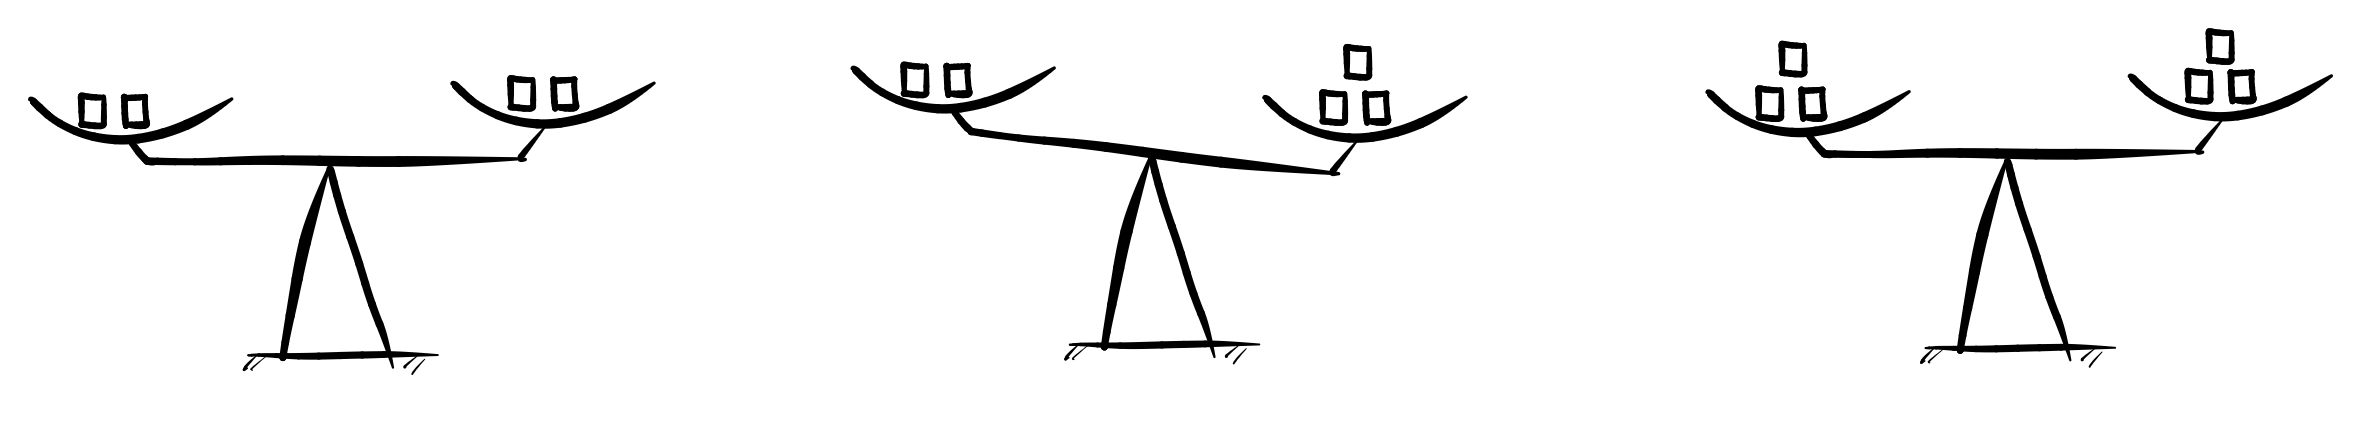
\includegraphics[width=0.8\linewidth]{imagensmecanica/balancapratos01.jpeg}
\captionof{figure}{A balança permanece em equilíbrio caso se adicione a mesma quantidade dos dois lados.}
\label{fig_mec_balanca01}
} 
\vspace{0.3cm}

Perceba que isso é verdade independente da balança estar ou não em equilíbrio, como é mostrado na Figura \ref{fig_mec_balanca02}, para uma balança inicialmente desequilibrada, com 2 pesos do lado direito e apenas 1 do lado esquerdo. Se adicionarmos 1 peso de um lado e nenhum do outro, então a configuração inicial da balança certamente será perturbada, como mostra a imagem do centro de tal figura. Contudo, se, mais uma vez, adicionarmos a mesma quantidade dos dois lados da balança, então a configuração inicial não é alterada, como o leitor pode perceber comparando a primeira e a última imagem da Figura \ref{fig_mec_balanca02}.
\vspace{0.3cm}

{
\centering
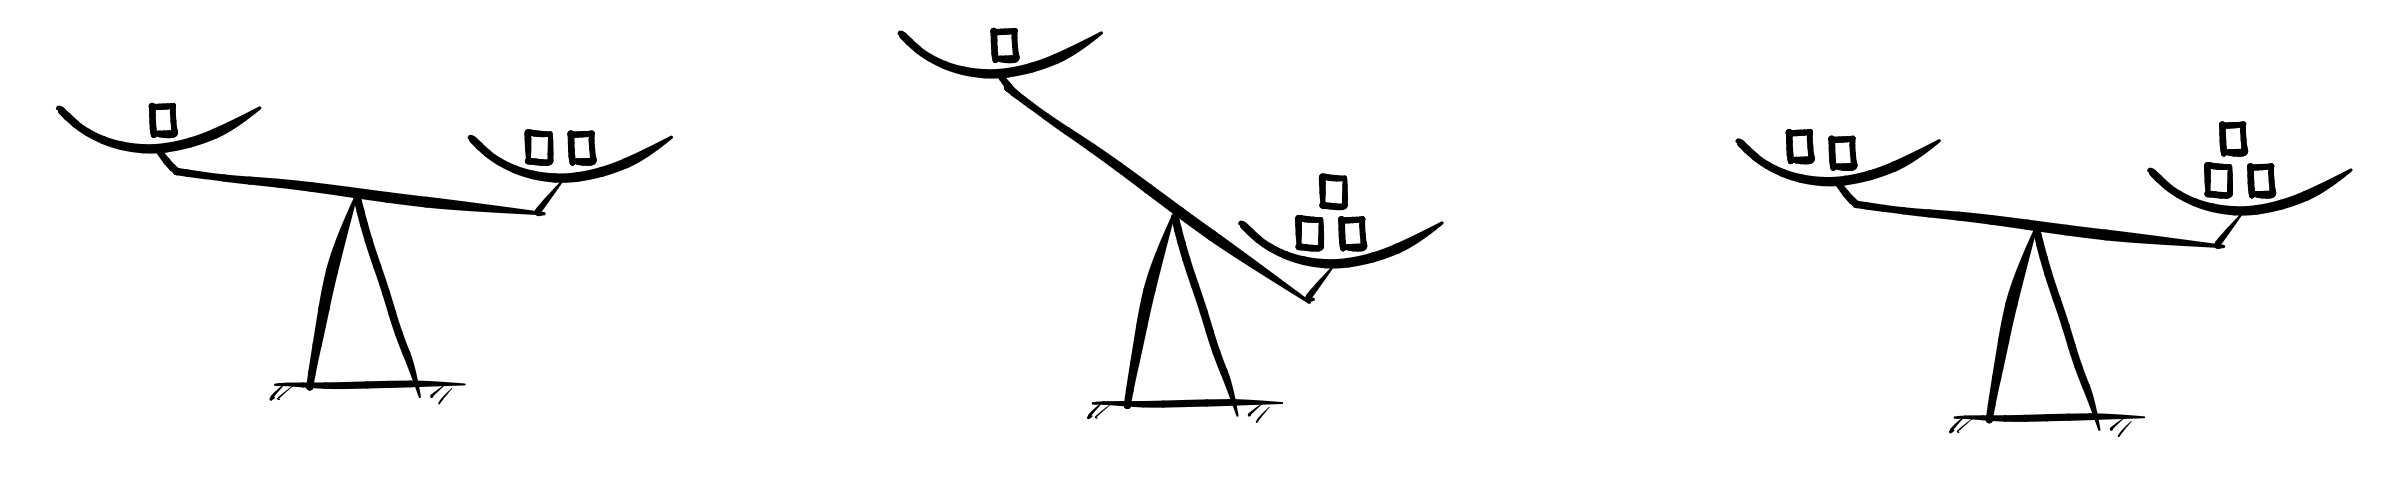
\includegraphics[width=0.8\linewidth]{imagensmecanica/balancapratos02.jpeg}
\captionof{figure}{A balança permanece na mesma configuração inicial caso se adicione a mesma quantidade dos dois lados.}
\label{fig_mec_balanca02}
} 

Sim, caro leitor -- a nossa conversa não tem absolutamente nada a ver com balanças. A ideia aqui é apenas usar esta analogia para extrair um princípio que utilizaremos aqui: em alguns contextos físicos, se adicionarmos a mesma quantidade a todos os elementos deste contexto -- no caso, os pratos da balança -- a física não é alterada, isto é, o sistema não é perturbado ou modificado.

Vamos agora ao nosso problema: Aristóteles está de carro, se movendo para a direita com uma velocidade $v_A=20$ m/s, enquanto Bohr se move em sentido contrário, com velocidade $v_B=30$ m/s.


{
\centering
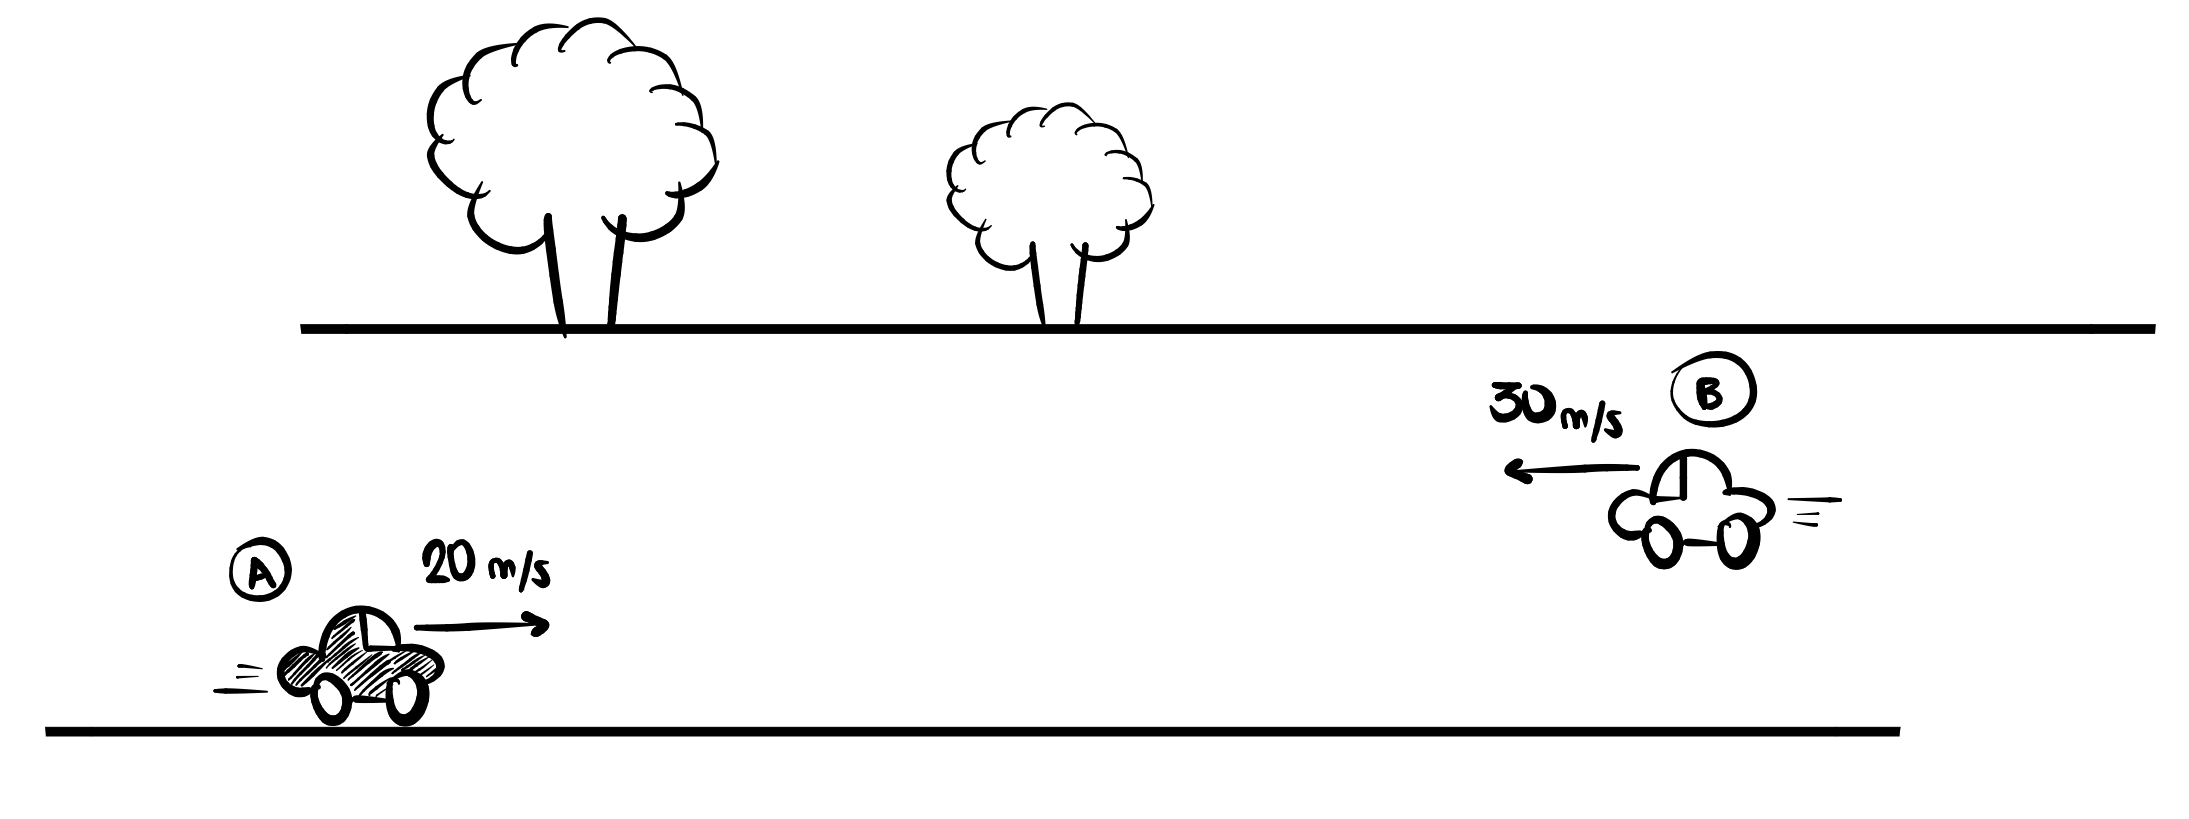
\includegraphics[width=0.6\linewidth]{imagensmecanica/velrelativaemudancaderefAB1.jpeg}
\captionof{figure}{Velocidades de $A$ e $B$ no referencial das árvores (terra).}
\label{velrelativaemudancaderefAB1}
} 
\vspace{0.3cm}

Note que não foi especificado em relação a qual referencial tais velocidades são medidas, de modo que assumimos que se trata da terra, como mostra a Figura \ref{velrelativaemudancaderefAB1}. Digamos que nosso interesse é o de obter a leitura do contexto no referencial de Bohr, ou seja, no referencial no qual $B$ está parado. Ora, para parar o carro $B$, que se move a $30$ m/s para a esquerda, o natural seria adicionar nele uma velocidade de $30$ m/s para a direita, o que anularia a sua velocidade e o colocaria em repouso. 

Contudo, fazer isso alteraria a configuração da nossa ``balança'', de modo que, para que sejamos justos, devemos adicionar a mesma coisa a todos os elementos do sistema; ou seja: adicionaremos uma velocidade de $30$ m/s para a direita a todos os corpos do nosso sistema, como mostra a Figura \ref{velrelativaemudancaderefAB2}.

{
\centering
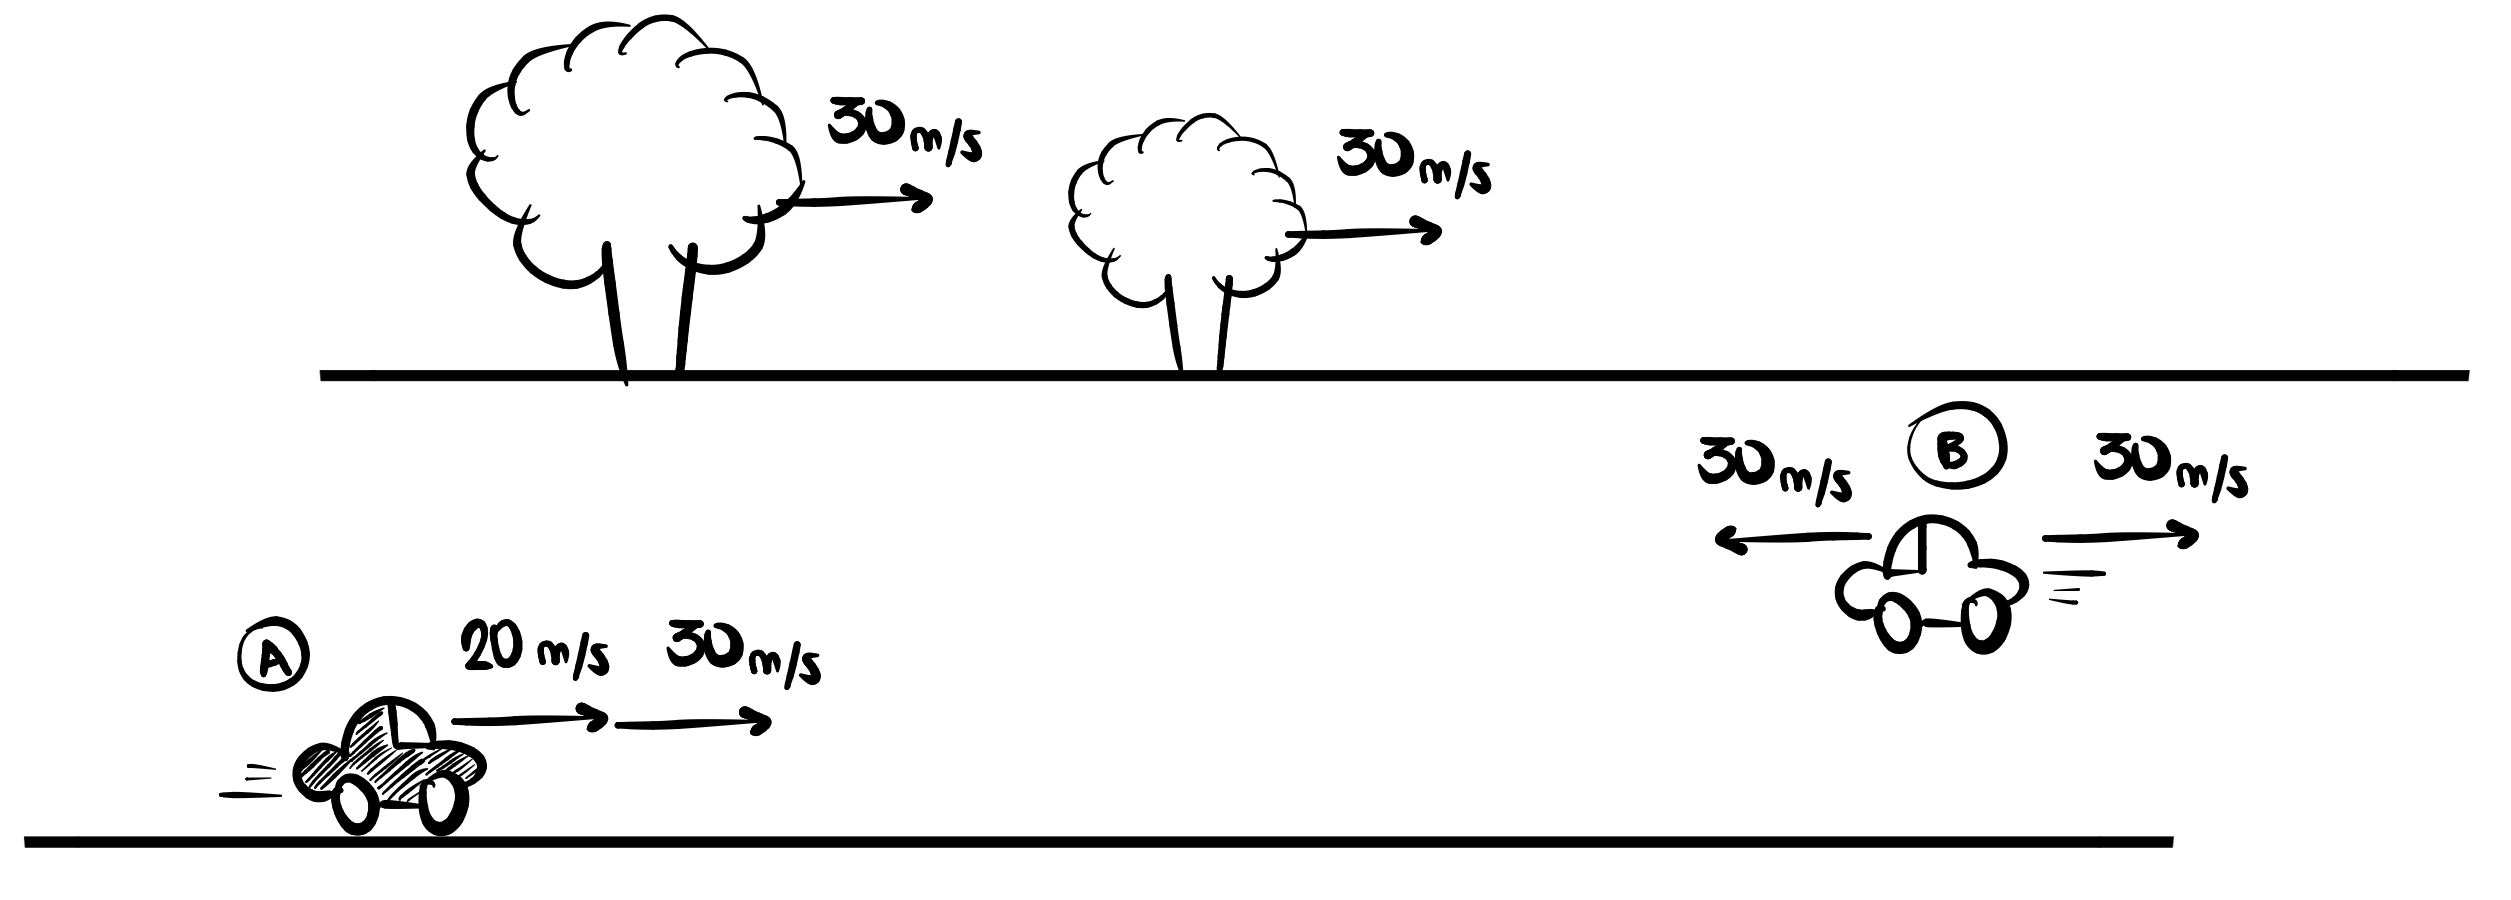
\includegraphics[width=0.6\linewidth]{imagensmecanica/velrelativaemudancaderefAB2.jpeg}
\captionof{figure}{Fazendo a mudança de referencial terra $\to$ B.}
\label{velrelativaemudancaderefAB2}
} 

Note que, ao sobrepor as velocidades, a velocidade do carro $B$ – 30 m/s para a direita sobreposta com 30 m/s para a esquerda – se anulará, que é justamente o que queríamos e o motivo de termos feito tal operação: estamos, agora, no referencial de Bohr. Este é o referencial no qual Bohr está parado. A Figura \ref{velrelativaemudancaderefAB3} mostra as velocidades finais dos corpos neste referencial: a velocidade de $A$ será de $20+30=50$ m/s e as velocidades das árvores serão de $30$ m/s para a direita.

{
\centering
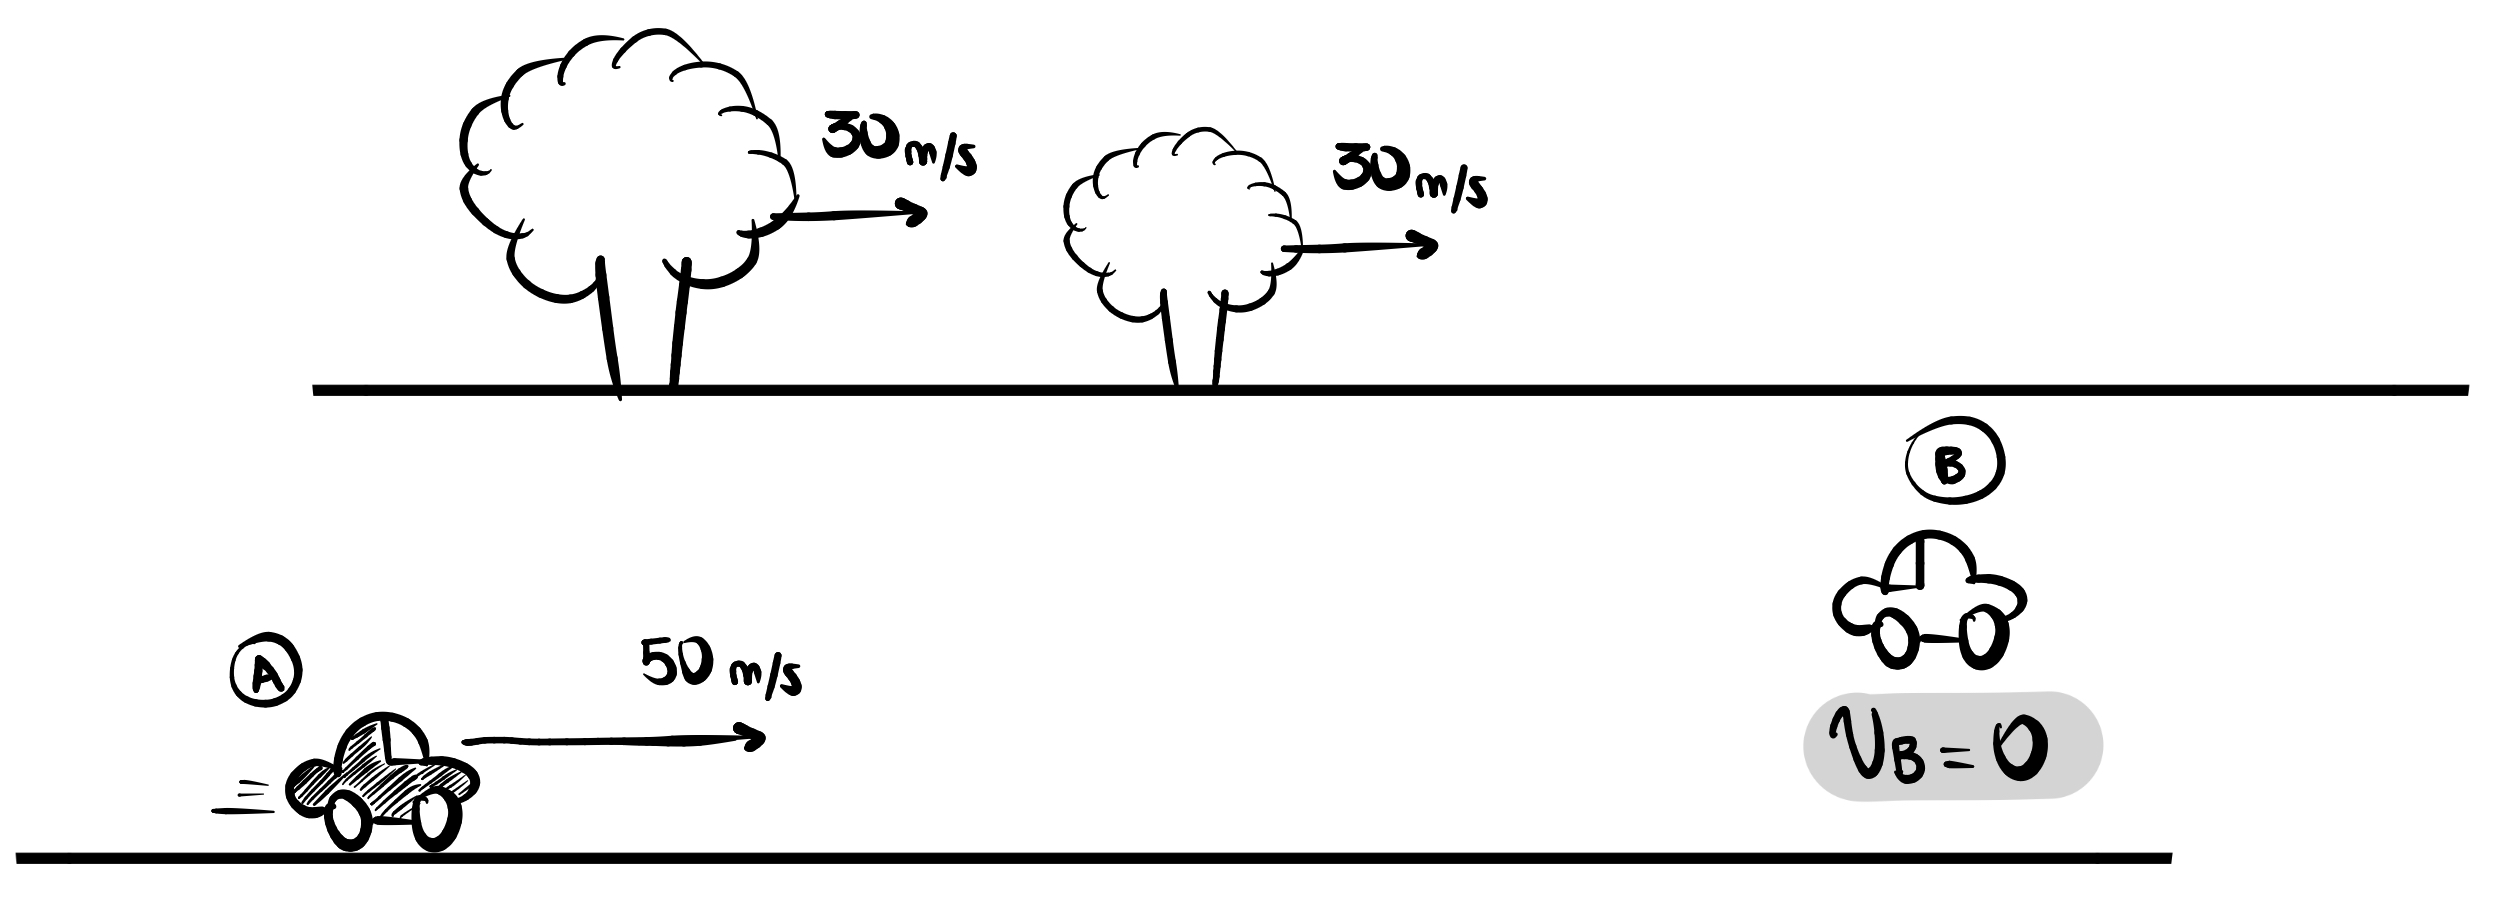
\includegraphics[width=0.6\linewidth]{imagensmecanica/velrelativaemudancaderefAB3.jpeg}
\captionof{figure}{Velocidades no referencial de $B.$}
\label{velrelativaemudancaderefAB3}
} 
\vspace{0.3cm}

O conceito de velocidade de uma árvore pode parecer um pouco estranho, mas vamos ler e comparar as situações físicas. Neste momento, é bem importante que o leitor observe e compare a Figura \ref{velrelativaemudancaderefAB1}, que mostra o problema no referencial das árvores, com a Figura \ref{velrelativaemudancaderefAB3}, que mostra o problema no referencial de $B.$ Note que, no referencial das árvores, elas estão paradas e o carro $B$ se aproxima delas a uma taxa de $30$ m/s a cada segundo. Já no referencial do carro $B$ é ele quem está parado e são as árvores que passam por ele a $30$ m/s. Razoável, não? Quando vocês está de carro, em uma estrada, não é essa a percepção que você tem -- de que as árvores estão passando por você e ficando para trás a uma alta velocidade?

Pois bem. Note que a física é a mesma, só muda a perspectiva: no referencial da árvore ela está parada e o carro passa por ela; no referencial do carro ele está parado e as árvores passam por ele. Tudo na mesma taxa de $30$ m/s, naturalmente -- a física não foi modificada, só estamos mudando de perspectiva.

Note, na Figura \ref{velrelativaemudancaderefAB1}, no referencial das árvores, que a cada segundo que passa o carro $A$ se aproxima 20 metros de $B$, e o carro $B$, que também se move em direção a $A$, se aproxima deste, portanto, de $30$ metros neste mesmo segundo. Ou seja, podemos dizer que, a cada segundo, a distância entre os carros $A$ e $B$ diminui de 50 metros. Essa é a leitura no referencial das árvores. Já observando a Figura \ref{velrelativaemudancaderefAB3}, notamos que o carro $B$ se encontra parado e o carro $A$ se aproxima dele a $50$ m/s: de novo, trata-se da mesma física, apenas vista por uma perspectiva diferente. Tal figura mostra todas as velocidades no referencial de $B.$

Vimos, neste caso, que sendo $v_A=20$ m/s a velocidade de $A$ em relação à terra e $v_B=30$ m/s a velocidade de $B$ em relação à terra, ao fazermos a mudança de referencial, obtivemos que a velocidade $v_{AB}$ do carro $A$ em relação ao carro $B$ era dada por

$$ \boxed{v_{AB}=v_A+v_B = 20+30=50 \text{ m/s.}}$$

Em resumo, para obtermos a velocidade de $A$ em relação a um referencial $B$, ou seja, para operarmos uma mudança de referencial, dois pontos merecem ser destacados, haja vista que todo o processo se sustenta neles:

\begin{enumerate}
    \item [(i)] Resolver o problema no referencial de $B$ é resolver o problema no qual $B$ está parado.

    \item [(ii)] A fim de parar um certo corpo, digamos $B,$ adiciona-se o oposto de sua velocidade a todos os corpos do sistema. Após efetuar a sobreposição de velocidades, a velocidade de $B$ será zero -- que é o que queríamos fazer -- de modo que estaremos no referencial de $B$: teremos, agora, as velocidades dos demais corpos no referencial de $B.$
\end{enumerate}


Poderíamos, por exemplo, a partir da situação da Figura \ref{velrelativaemudancaderefAB1}, escolher parar o carro $A$ para observar o problema na perspectiva de Aristóteles. Lembre-se que o referencial de Aristóteles é o referencial no qual ele está parado, por isso buscaremos zerar a velocidade de $A.$ Para isso, como ele se move a $20$ m/s para a direita, adicionaremos a velocidade de $20$ m/s para a esquerda a todas as partículas do sistema, como mostra a Figura \ref{velrelativaemudancaderefAB5}. Perceba que a velocidade de Aristóteles agora será, naturalmente, nula. A velocidade de $B$ em relação a $A$ será dada pela sobreposição das duas velocidades, ou seja $20+30=50$ m/s.

\vspace{0.3cm}
{
\centering
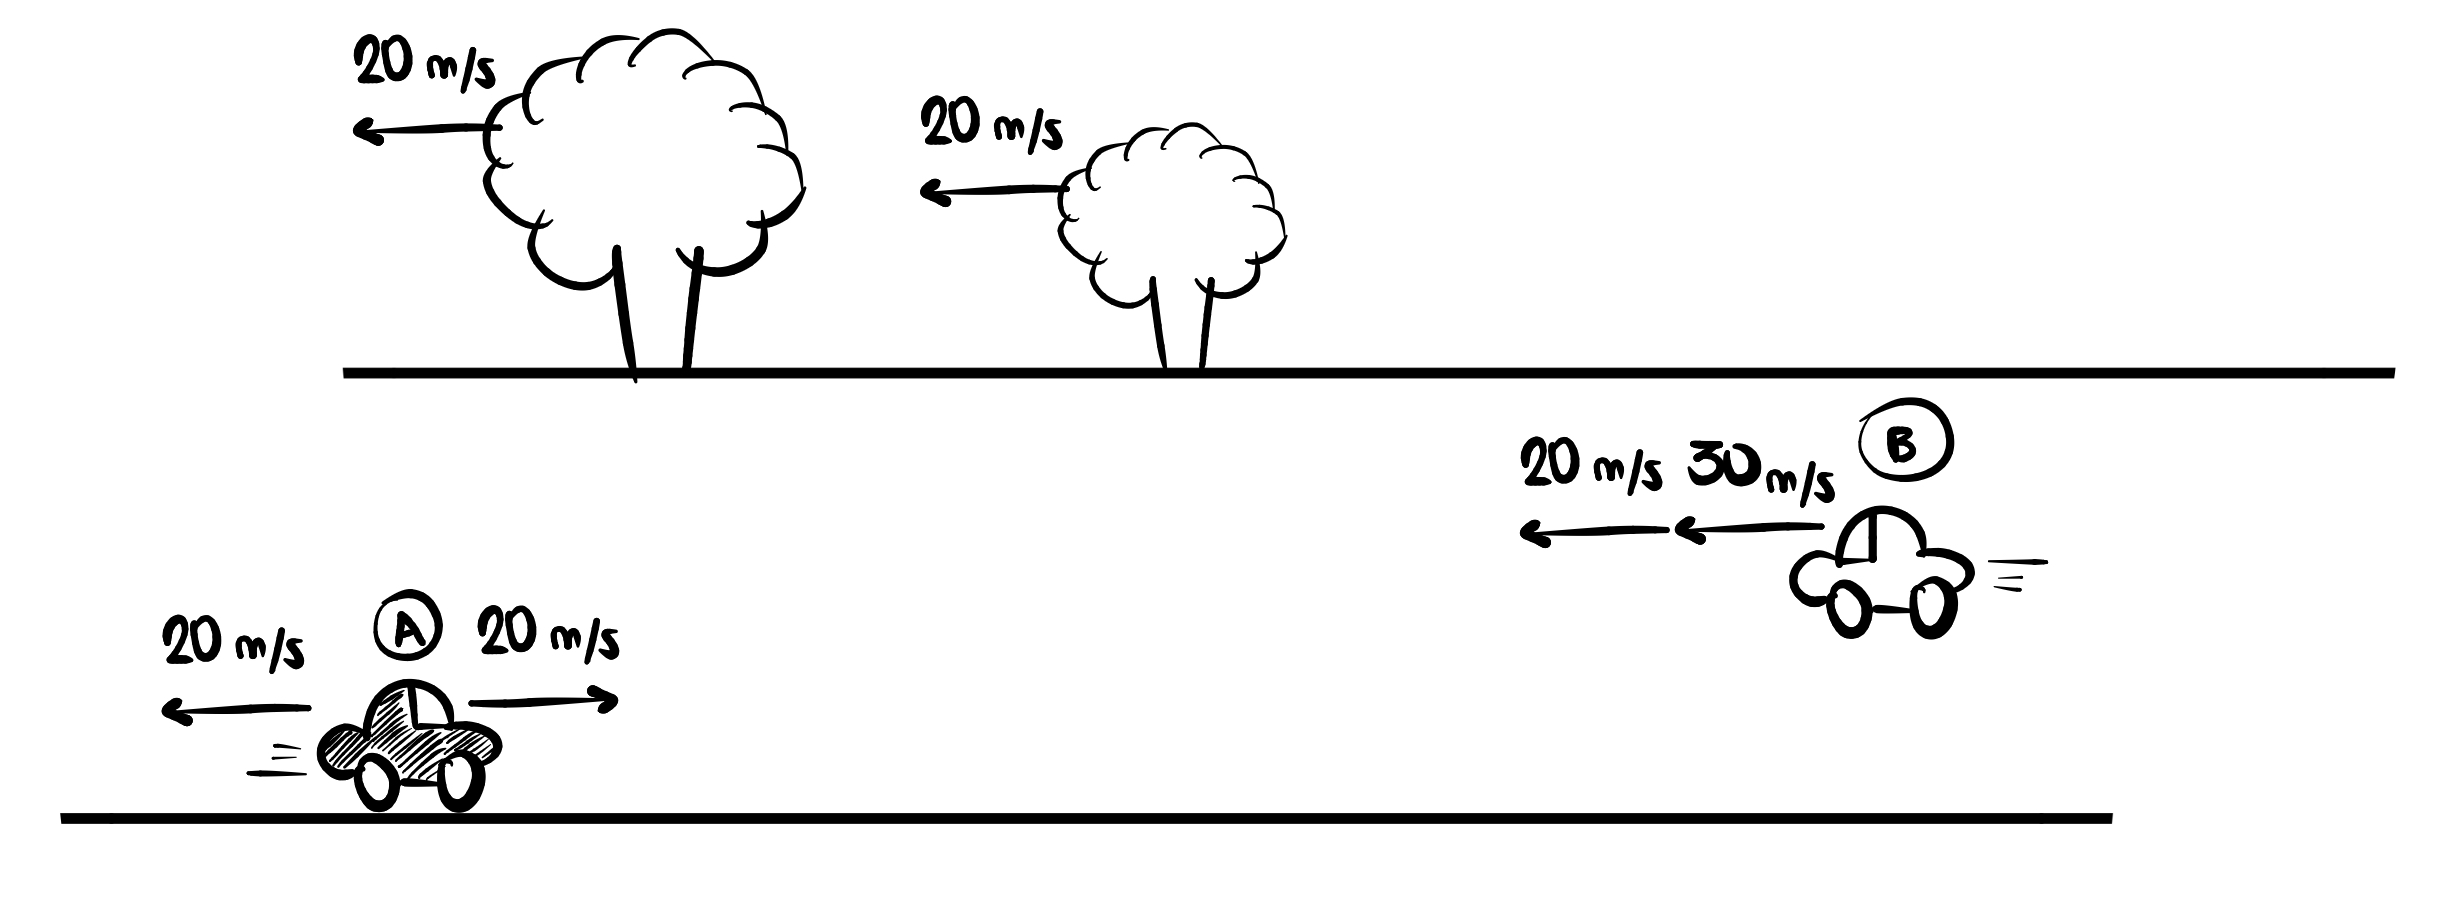
\includegraphics[width=0.6\linewidth]{imagensmecanica/velrelativaemudancaderefAB5.jpeg}
\captionof{figure}{Fazendo a mudança de referencial terra $\to$ A.}
\label{velrelativaemudancaderefAB5}
} 
\vspace{0.3cm}

Por fim, a Figura \ref{velrelativaemudancaderefAB4} mostra a situação final no referencial de $A.$ Perceba que nossa leitura é bem parecida: no referencial da terra as árvores estão paradas e o carro $A$ passa por elas a uma velocidade de $20$ m/s; já no referencial de $A$ é ele quem está parado e as árvores passam por ele a uma velocidade de $20$ m/s.

No referencial das árvores (terra) a distância entre $A$ e $B,$ como analisamos anteriormente, encurtava de $50$ metros a cada segundo; já no referencial de $A$ vemos que ele está parado enquanto $B$ se aproxima dele a $50$ metros por segundo -- a mesma Física, apenas vista por perspectivas diferentes.

{
\centering
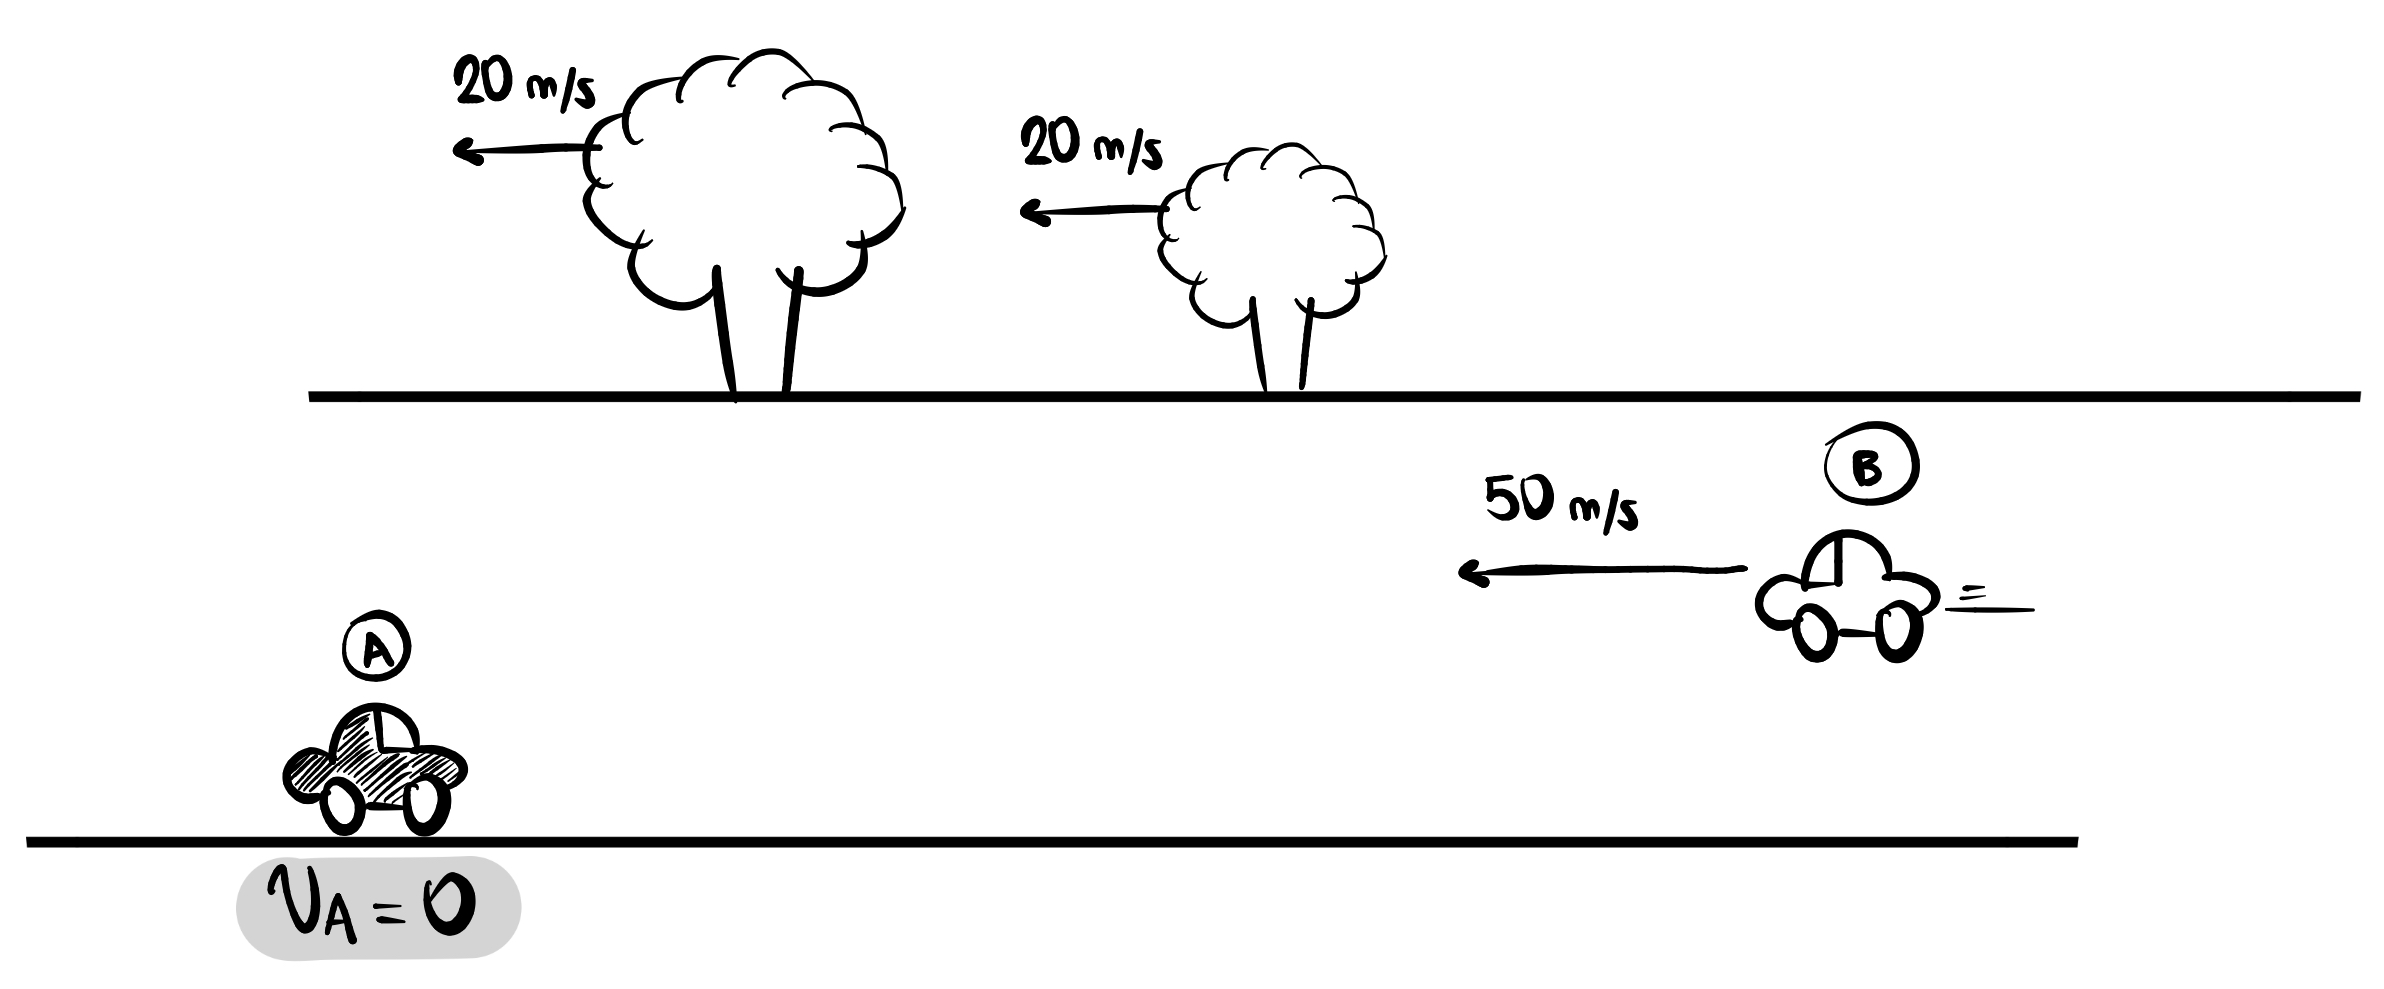
\includegraphics[width=0.6\linewidth]{imagensmecanica/velrelativaemudancaderefAB4.jpeg}
\captionof{figure}{Velocidades no referencial de $A.$}
\label{velrelativaemudancaderefAB4}
}    
\vspace{0.3cm}
Sugiro que o leitor tente mudar para o referencial de $A$, como exercício, a partir da situação da Figura \ref{velrelativaemudancaderefAB3}, isto é, do referencial de $B.$ \footnote{Dica: para fazer isso basta perceber que, para anular a velocidade de $A,$ é necessário adicionar uma velocidade de $50$ m/s para a esquerda em todos os corpos do sistema.} Após fazê-lo, observe a simetria entre $A$ e $B$ pelas Figuras \ref{velrelativaemudancaderefAB3} e  \ref{velrelativaemudancaderefAB4}: no referencial de $B$ ele está parado, e $A$ se aproxima dele a $50$ m/s. Já no referencial de $A$ é ele quem está parado, e $B$ se aproxima dele a $50$ m/s -- perceba, mais uma vez, como a física concorda. São apenas leituras de referenciais distintos. Ou seja, estamos aqui concluindo que

$$ v_{AB} = v_{BA},$$

\noindent ou seja, a velocidade $v_{AB}$ de $A$ em relação a $B$ é exatamente a mesma, em valor absoluto, que a velocidade $v_{BA}$ de $B$ em relação a $A$ -- as duas foram obtidas somando os valores $v_A$ e $v_B$ das velocidades de $A$ e $B$ em relação às árvores.

O leitor poderia, como exercício, considerar um contexto como o da Figura \ref{velrelativaemudancaderefAB1}, porém com $B$ se movendo para a direita, no mesmo sentido de $A.$ Fazendo a mudança de referencial da terra para o referencial de $A$ ou de $B$, será possível obter a velocidade $v_{AB}$ de $A$ em relação a $B$ (ou a velocidade $v_{BA}$ de $B$ em relação a $A,$ mas já sabemos que essas duas coisas são iguais), de modo que será possível compreender de onde vem o sinal negativo na Equação \eqref{mecanica_eq_velocidaderelativa}.

Por fim, para obtermos de forma geral a Equação \eqref{mecanica_eq_velocidaderelativa}, convido o leitor a observar a Figura \ref{vrelsentidooposto}. Não vou me delongar aqui e deixarei o leitor observar a figura e pensar por si só -- note apenas que, na primeira imagem temos a situação no referencial das árvores, na imagem central temos a operação da mudança de referencial e na última imagem temos a situação no referencial de $B.$

{
\centering
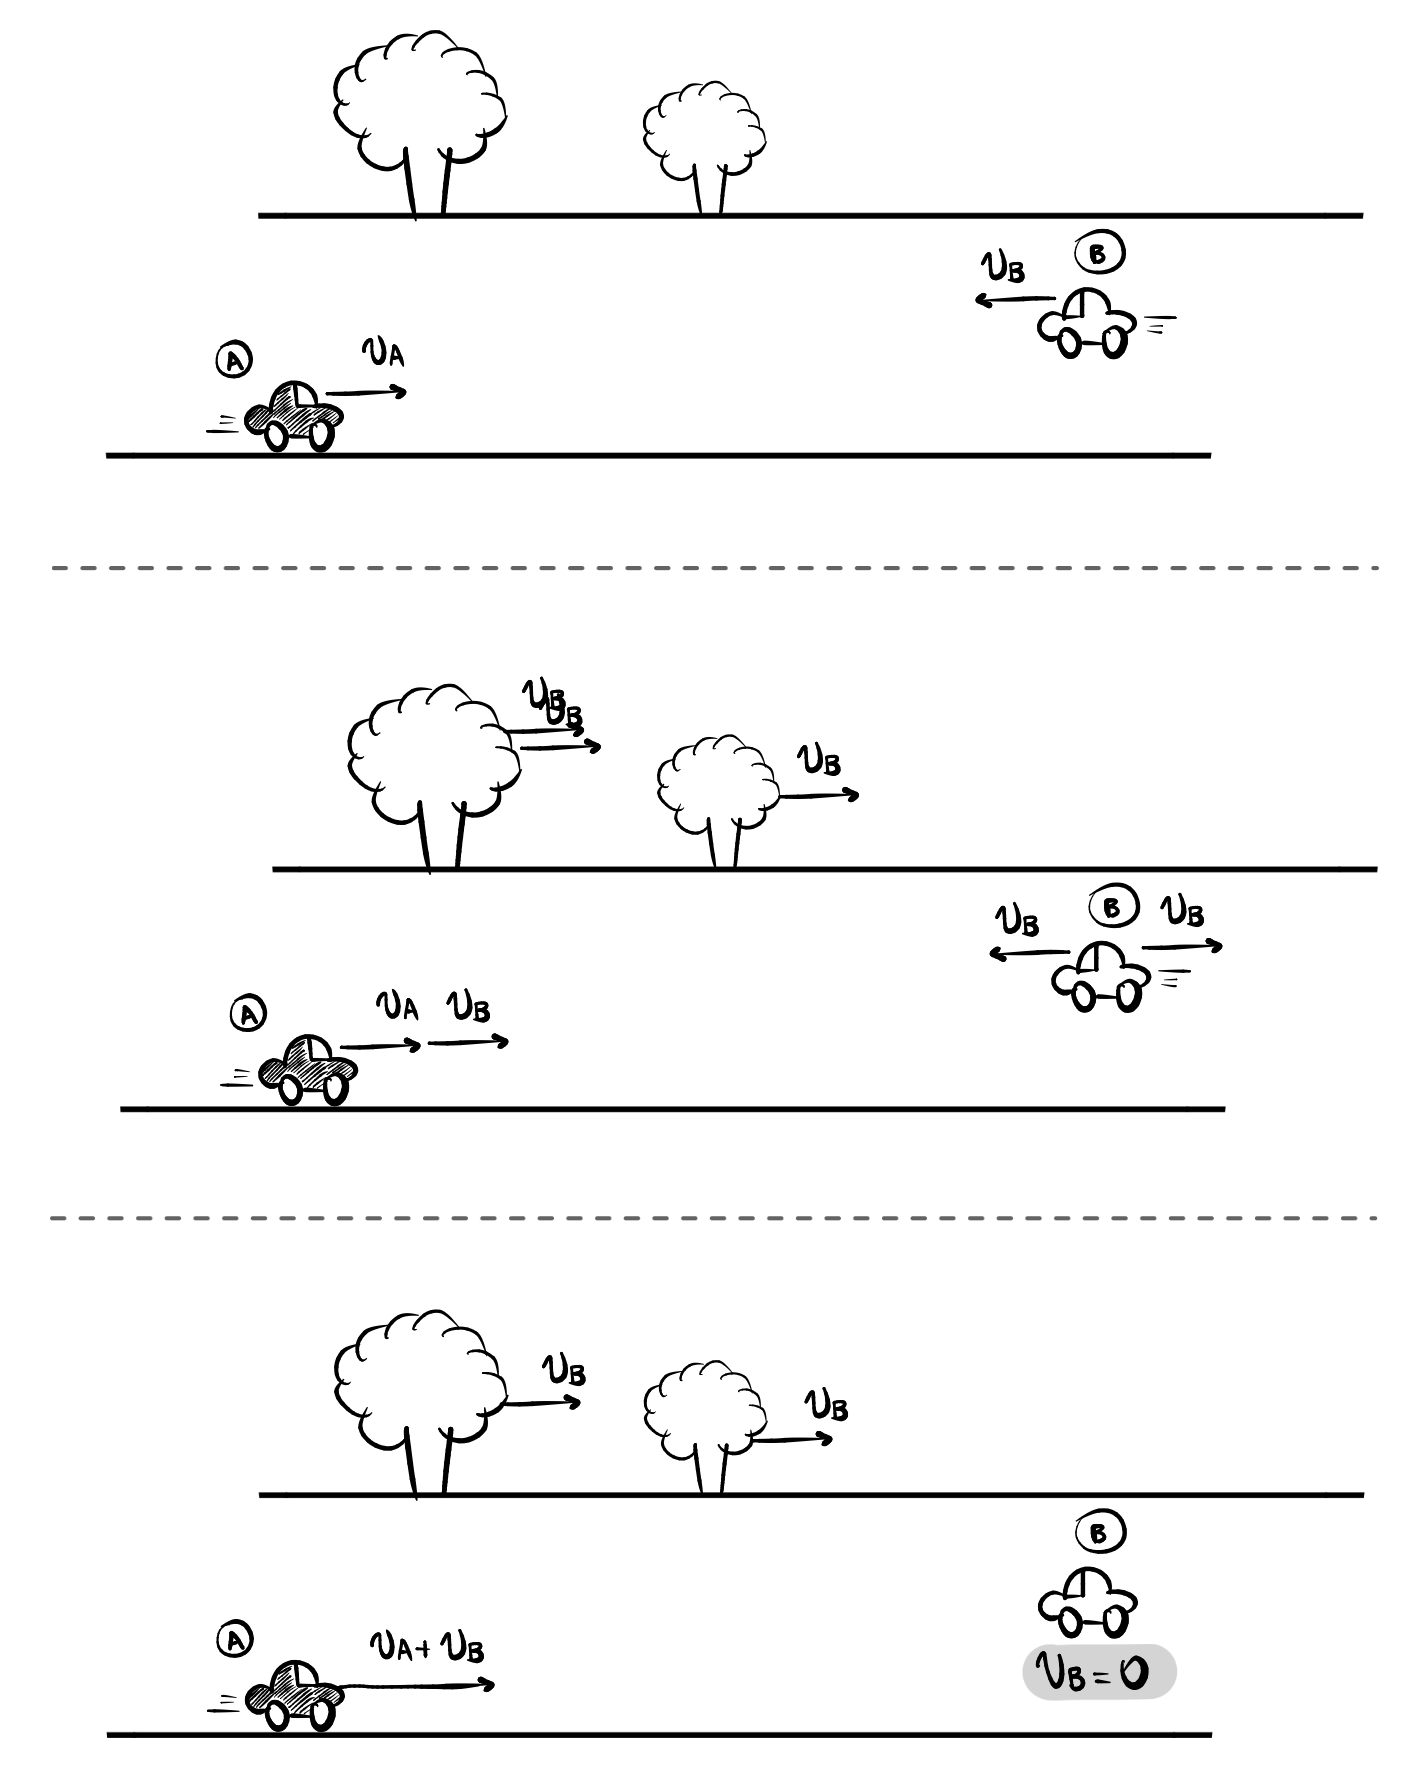
\includegraphics[width=0.6\linewidth]{imagensmecanica/vrelsentidooposto.png}
\captionof{figure}{Obtenção da velocidade relativa $v_{AB}$ de $A$ em relação a $B$ quando os dois corpos se movem na mesma direção mas em sentido contrários.}
\label{vrelsentidooposto}
}    
\vspace{0.3cm}
A partir de tal figura, o leitor concluirá que, sempre que dois carros se moverem na mesma direção mas em sentidos opostos, a velocidade de um em relação ao outro (ou do outro em relação ao um -- o que dá na mesma) será dada pela soma das suas velocidades, isto é, se $v_A$ e $v_B$ são as velocidades de $A$ e $B$ em relação à estrada, então a velocidade de $A$ em relação $B$ será dada por

$$ \boxed{v_{AB}=v_A+v_B.}$$

Já a Figura \ref{vrelsentidoigual} mostra a mesma situação, porém para os corpos que se movem no mesmo sentido -- a primeira imagem mostra a situação no referencial das árvores, na imagem central temos a operação da mudança de referencial e na última imagem temos a situação no referencial de $B.$


{
\centering
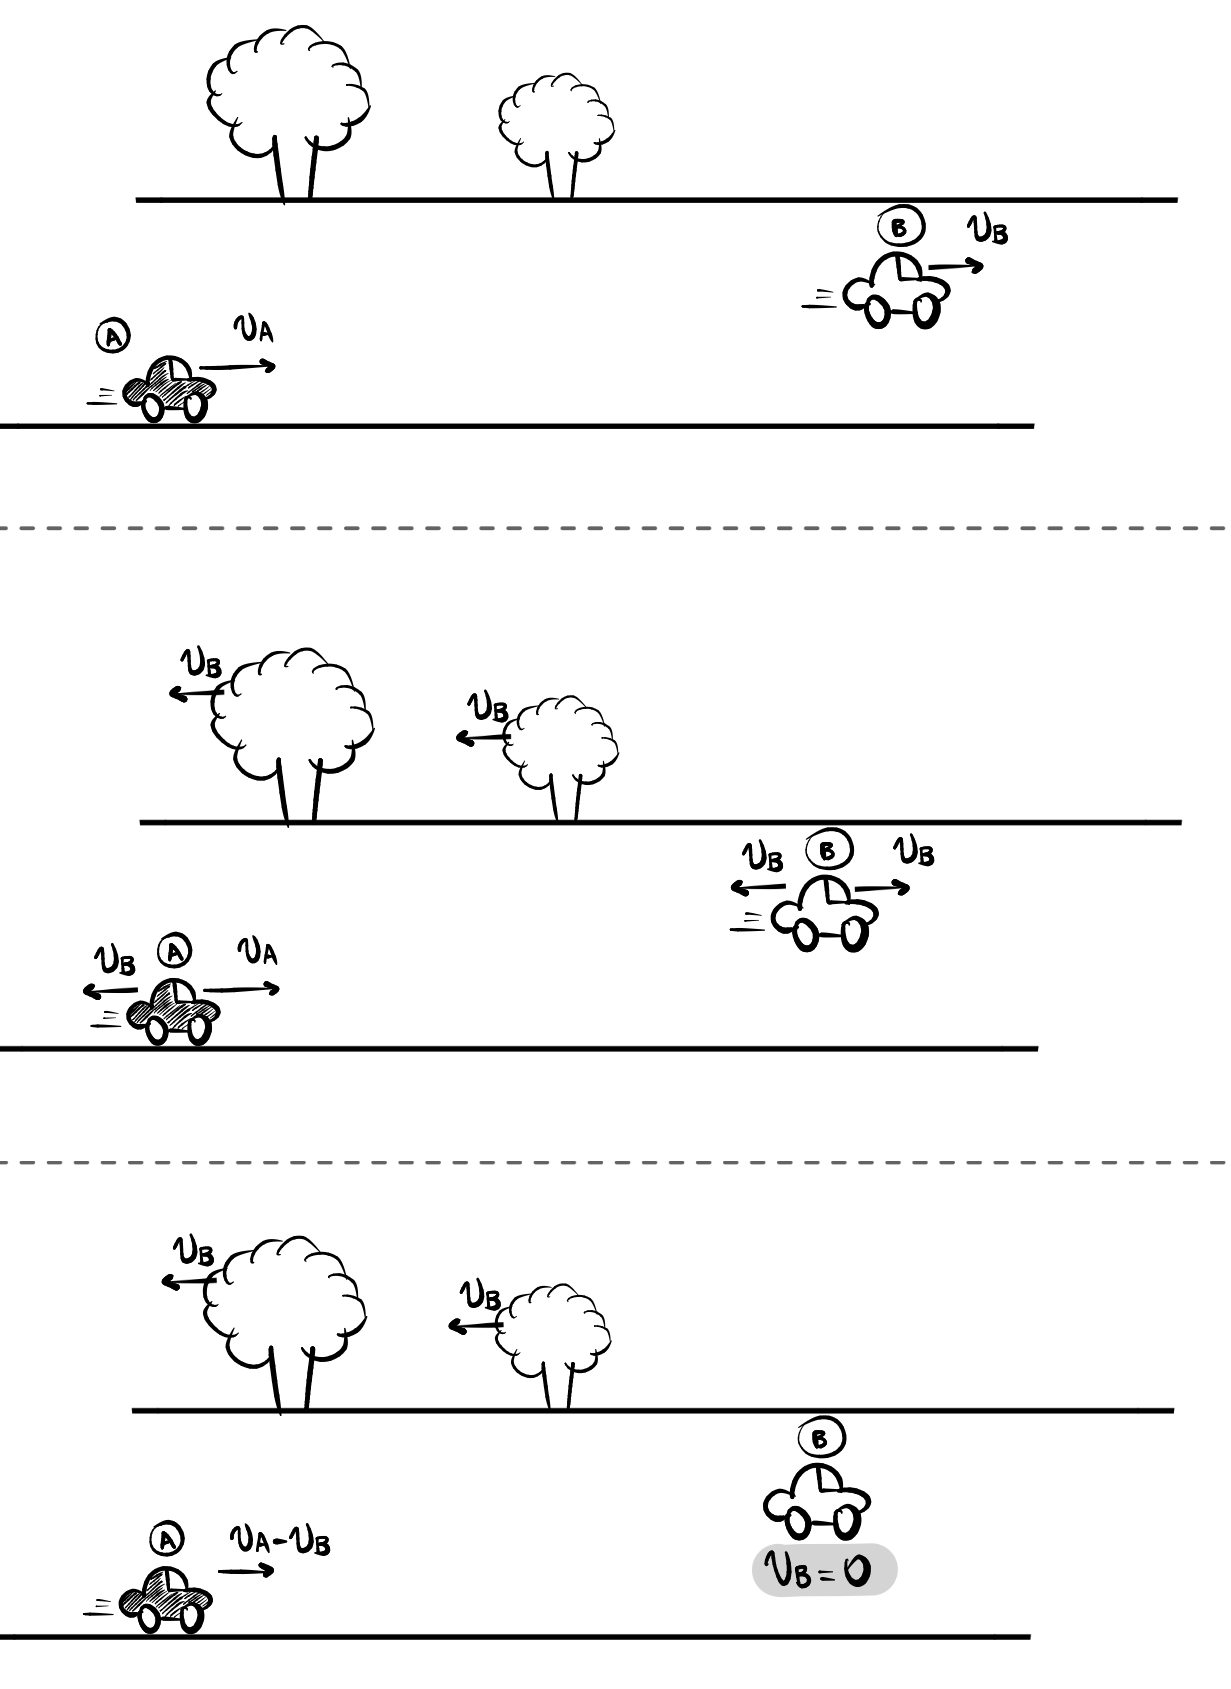
\includegraphics[width=0.5\linewidth]{imagensmecanica/vrelsentidoigual.jpeg}
\captionof{figure}{Obtenção da velocidade relativa $v_{AB}$ de $A$ em relação a $B$ quando os dois corpos se movem na mesma direção e mesmo sentido.}
\label{vrelsentidoigual}
}    
\vspace{0.3cm}
Dessa análise, o leitor concluirá que, sempre que dois carros se moverem na mesma direção e mesmo sentido, a velocidade de um em relação ao outro será dada pela diferença de suas velocidades, isto é, se $v_A$ e $v_B$ são as velocidades de $A$ e $B$ em relação à estrada, então a velocidade de $A$ em relação $B$ será dada por

$$ \boxed{v_{AB}=v_A-v_B.}$$

A Equação \eqref{mecanica_eq_velocidaderelativa} sintetiza as duas conclusões acima tiradas. Espero que, com toda essa discussão aqui feita, o leitor não se contente em apenas memorizar tal equação, mas compreenda, com profundidade, a sua natureza -- a operação de mudança de referencial.

\secgfe{Onde é usada}

Como dito anteriormente: toda velocidade é relativa. Qualquer velocidade dada sempre é em relação a algum sistema de referência específico; logo, o conceito de velocidade relativa é usado basicamente em qualquer contexto em que se fale de velocidade. Contudo, usar diretamente a Equação \eqref{mecanica_eq_velocidaderelativa} é um recurso do qual lançaremos mão quando quisermos observar o problema na perspectiva de outro referencial. Em muitos contextos, como veremos nos exemplos, fazer uma mudança de referencial simplifica drasticamente a matemática para resolver o exercício.


\secgfe{Erros comuns}

O erro mais comum aqui é o estudante se ater a memorizar a Equação \eqref{mecanica_eq_velocidaderelativa} sem entender o que de fato está por trás dela: uma mudança de referencial. Para o estudante que entendeu em detalhes o desenvolvimento feito na seção anterior, não só ficará totalmente dispensável memorizar a equação em questão, como ele terá muito mais profundidade e domínio acerca do que está fazendo quando usar o conceito de velocidade relativa.


\secgfe{Observações}

O conceito que construímos aqui é muito mais amplo do que o contexto no qual o aplicamos. A ideia de que estudar o problema no referencial $X$ é avaliar o problema na perspectiva na qual $X$ está parado -- e, portanto, para pará-lo, basta adicionar o oposto da sua velocidade à todas as partículas do sistema -- é um conceito que valerá para movimentos bidimensionais ou mesmo tridimensionais. É claro que, em tais movimentos, como estudaremos na Cinemática Vetorial, o tratamento geométrico para operar uma mudança de referencial pode ser um pouco mais complicado, mas, ainda assim, o princípio será exatamente o mesmo.

Sendo assim, cabe a observação de que o princípio que aqui construímos é geral: \textbf{avaliar um problema físico no referencial de $A$ é estudar o problema no referencial no qual $A$ está parado. Para pará-lo, basta adicionar o oposto de sua velocidade à todas as partículas envolvidas no sistema.}


\vspace{0.3cm}


\begin{exemplo}[Nível I]\label{exemplo_cinematica_vrelativa01}

Dois carros, separados de $600$m um do outro, se movem um em direção ao outro. Se as suas velocidades são de $20$ m/s e $40$ m/s, após quanto tempo eles se encontram?


\resolucao


Esse é o problema mais clássico de toda a Cinemática e, com o desenvolver dos nossos estudos, veremos diferentes forma de resolvê-lo ao longo das próximas seções.\\

Perceba que o enunciado nos forneceu velocidades mas sequer disse em relação a quem elas são medidas. Como já conversamos, isso acaba sendo comum e, quando ocorre, devemos partir da premissa de que tais velocidades são em relação à terra -- em relação a um indivíduo parado, na estrada. \\

Em geral é sempre mais complicado resolver um problema como este se os dois carros estão se movendo. Desse modo, façamos uma mudança de referencial para parar um dos carros e tentar simplificar o problema. Seja $A$ o carro cuja velocidade é de $20$ m/s e $B$ o carro cuja velocidade é de $40$ m/s. A Figura \ref{fig_mec_mudancareferencialexemplo01} mostra a mudança de referencial para o carro $B:$ adicionamos uma velocidade de $40$ m/s para a direita em todas as partículas do sistema, de modo que a velocidade resultante de $B$ é zero -- estamos, portanto, no referencial do carro B -- e a velocidade resultante de $A$ é de $60$ m/s, como mostra última imagem da figura.

{
\centering
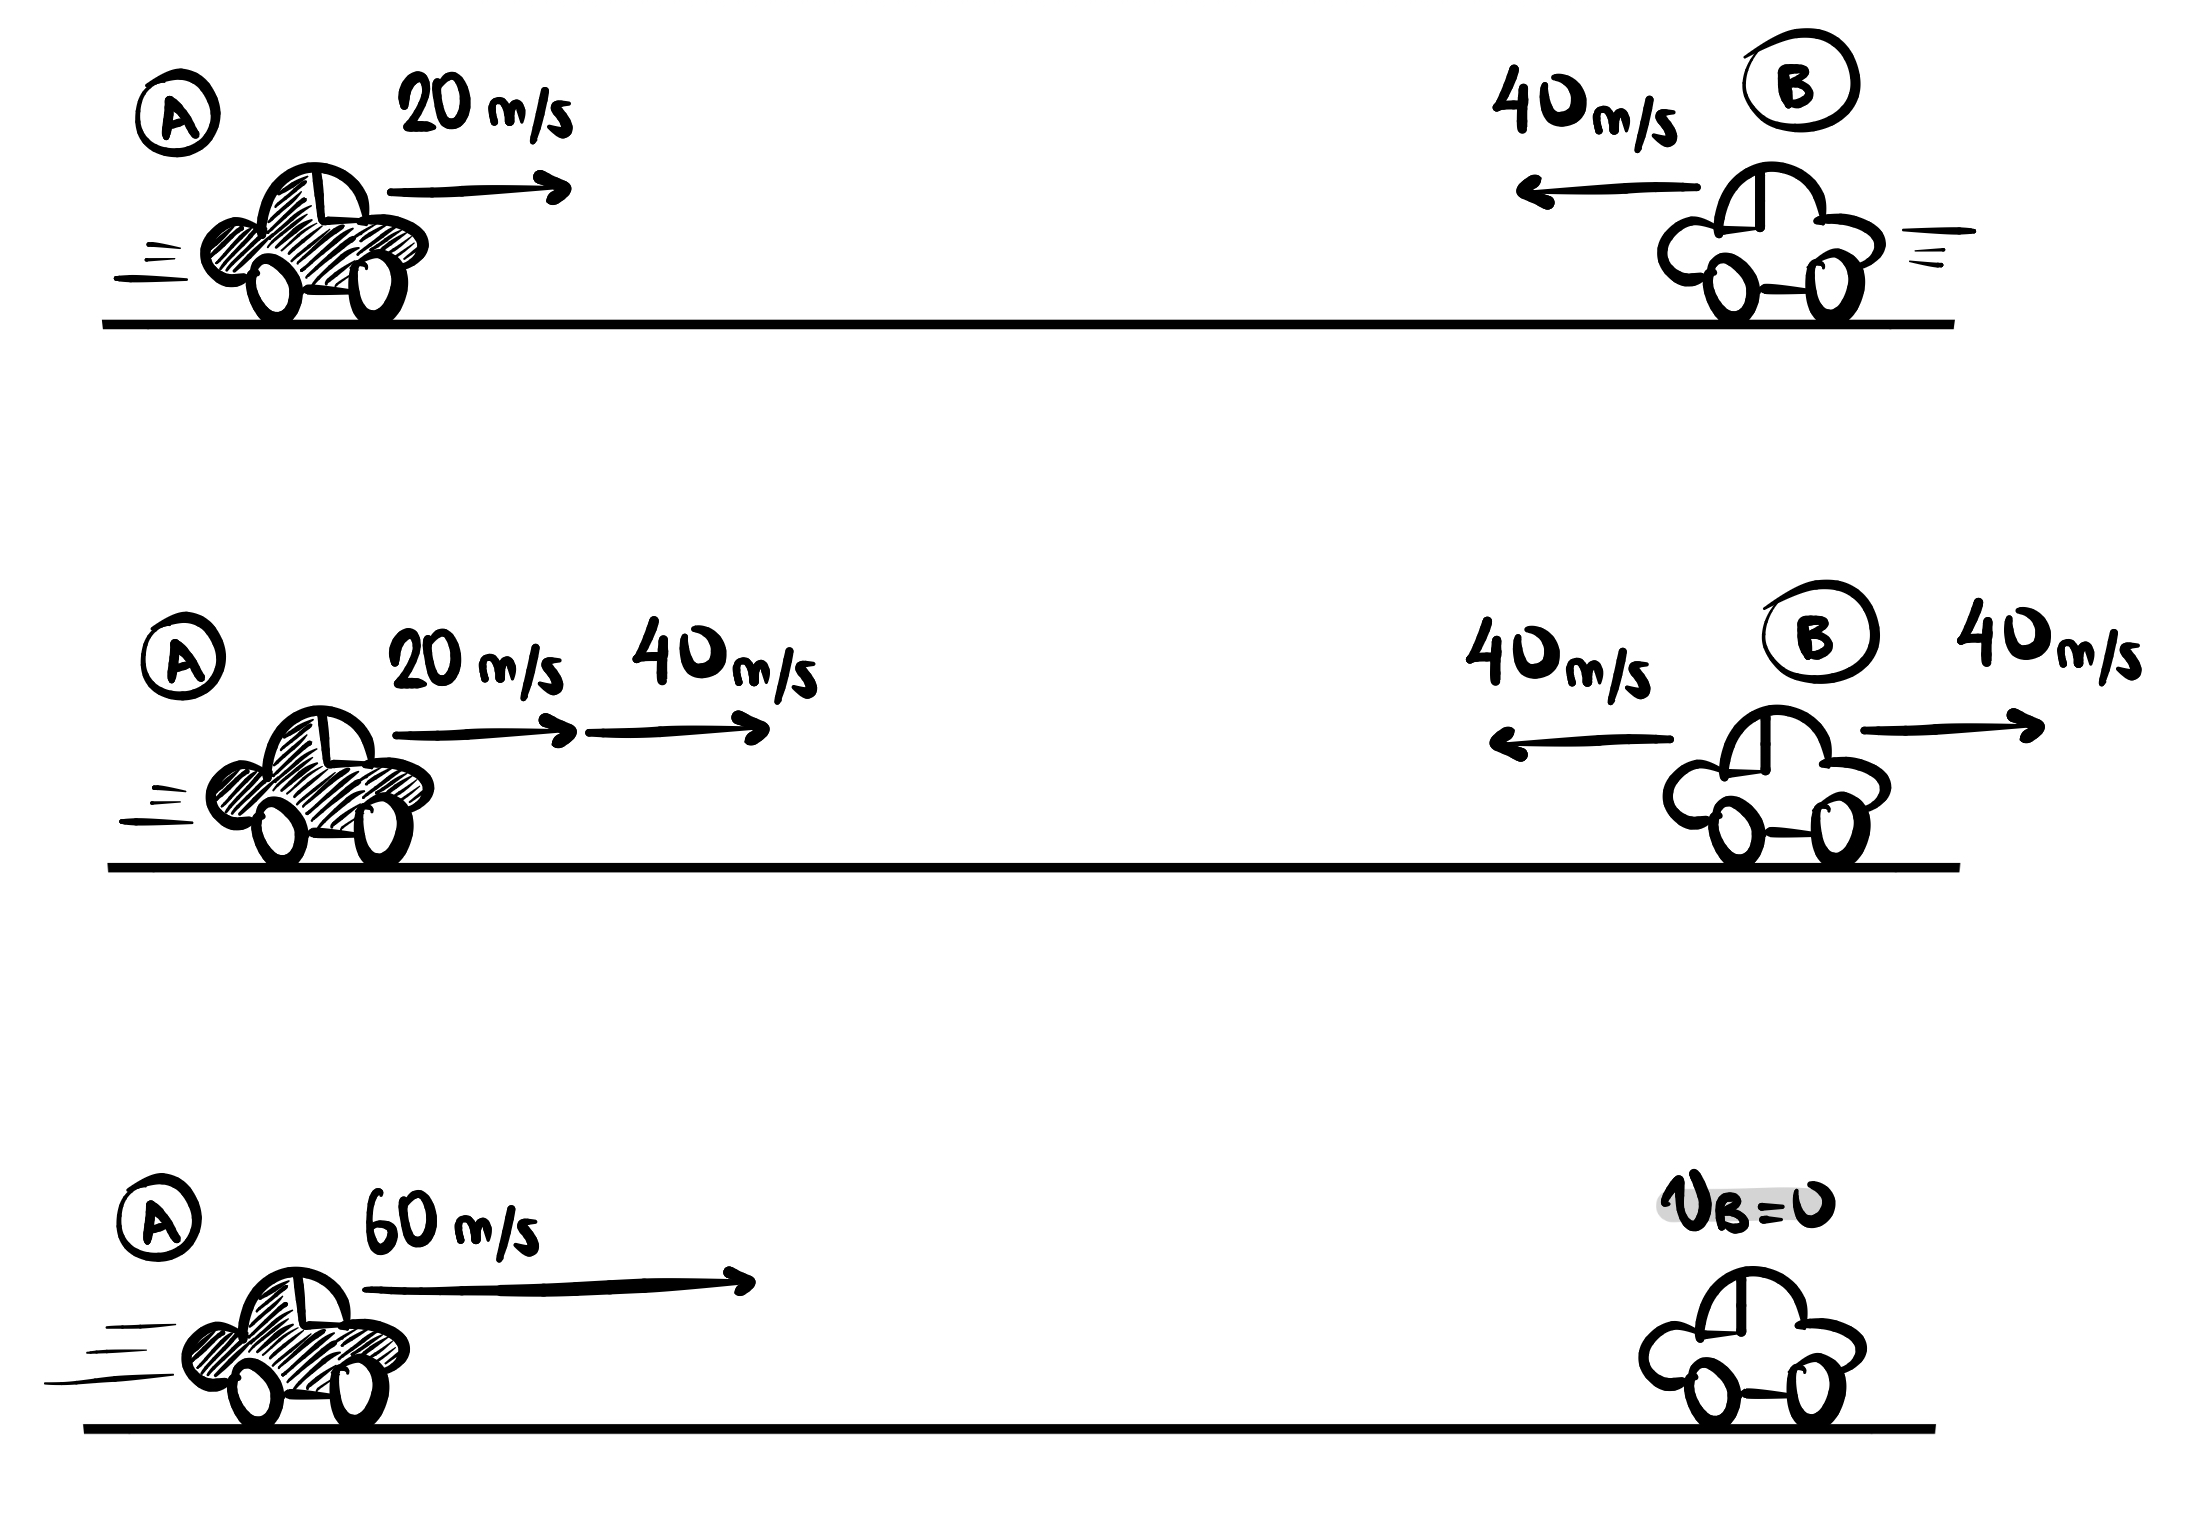
\includegraphics[width=0.5\linewidth]{imagensmecanica/mudancareferencialexemplo01.jpeg}
\captionof{figure}{Mudando do referencial da Terra para o referencial do carro B -- referencial no qual B está parado.}
\label{fig_mec_mudancareferencialexemplo01}
} 
\vspace{0.3cm}

Perceba como o problema agora se tornou mais fácil: temos dois carros, afastados um do outro de 600m. Um deles está parado, e o outro se aproxima dele a uma velocidade de $60$ m/s. O problema ficou tão simples que não é preciso muito mais conhecimento para perceber que, avançando $60$ metros a cada segundo, levar-se-á $10$ segundos para varrer os 600 metros que distanciam os dois carros. Logo, em $10$ segundos os carros terão se encontrado.

Como é a primeira vez que isso foi feito, cabe destacarmos alguns pontos importantes:

\begin{enumerate}
    \item [(i)] Alguém poderia pensar: \textit{``computamos que leva 10s para os carros se encontrarem, mas isso foi no referencial do carro $B.$ O que me garante que o tempo será o mesmo no referencial original, da terra?''}

    Seria uma boa pergunta -- e retornaremos a ela no futuro. Por hora, eu deixo ao leitor apenas a provocação: digamos que você e um amigo disparem um cronômetro em seus respectivos relógios, um ao lado do outro, no mesmo instante. Digamos que isso ocorre às 08 horas da manhã. Daí você pega um ônibus e vai à escola e, no fim do dia, digamos às 17 horas, retorna à casa de seu amigo. Ao comparar os tempos marcados nos cronômetros, em qual relógio terá passado mais tempo?

    Pois bem...se passaram-se 9 horas, isso parece ser algo absoluto, não? Algo que não depende do relógio que usamos para marcar, ou de qual referencial marcou a passagem do tempo...concorda?\footnote{Conheci um cara que discordava disso. Seu nome era Albert Einstein, mas isso é prosa para o outro volume da coleção...}

    \item [(ii)] Como já levantamos, essa não é a única forma de resolver o problema. Existem pelo menos outras duas ou três que veremos quando construirmos novas equações. Contudo, já adianto ao leitor, essa é a forma que o autor julga ser a melhor -- é que torna a situação e, consequentemente, os cálculos matemáticos, os mais simples de todos.
\end{enumerate}


\end{exemplo}



\vspace{0.3cm}






\begin{exemplo}[Nível II (UFMG - 2001)]\label{exemplo_cinematica_vrelativa02}

Um menino flutua em uma bóia que está se movimentando, levada pela correnteza de um rio. Uma outra bóia, que flutua no mesmo rio a uma certa distância do menino, também está descendo com a correnteza. A posição das duas bóias e o sentido da correnteza estão indicados na figura.


{
\centering
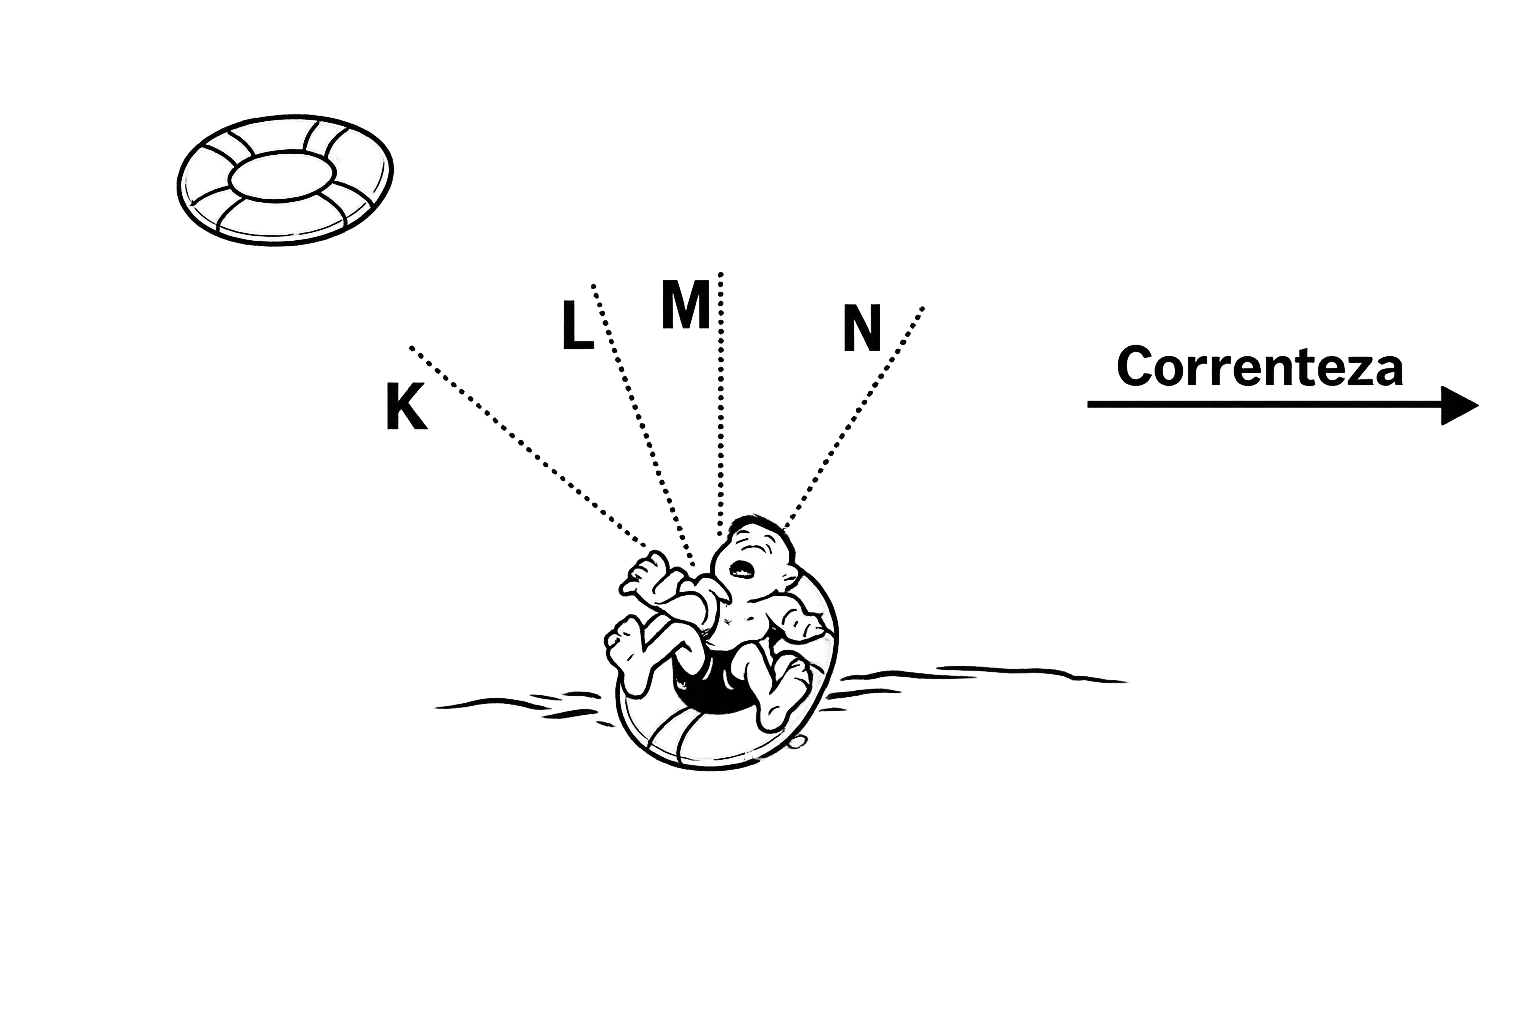
\includegraphics[width=0.50\linewidth]{imagensmecanica/ufmgboiarioexemplotest.png}
\captionof{figure}{}
\label{fig_mec_ufmgboiarioexemplo}
} 



Considere que a velocidade da correnteza é a mesma em todos os pontos do rio. Nesse caso, para alcançar a segunda bóia, o menino deve nadar na direção indicada pela linha:

\begin{enumerate}
  \item [(a)] K.
  \item [(b)] L.
  \item [(c)] M.
  \item [(d)] N.
\end{enumerate}


\resolucao

O problema, no referencial posto, parece ser mais complicado do que de fato é. Por hora, vamos imaginar que não há correnteza alguma -- as águas do rio são calmas e estão em repouso absoluto. Neste contexto, para qual direção o menino deve nadar para buscar a bóia? Parece óbvio que é na direção K -- a direção que liga o menino à bóia --, certo? \\

Pois bem. Agora quero convencer o leitor de que este é exatamente o caso. O enunciado nos diz que a velocidade da correnteza é a mesma em todos os pontos do rio, logo, a água do rio, a bóia e o menino se movem rio abaixo com a mesma velocidade -- a velocidade $v_c$ da correnteza, ou seja, a velocidade da água do rio. Observe agora a Figura \ref{fig_mec_ufmgboiarioexemplo02}, na qual, em sua primeira imagem, temos a ilustração da situação anteriormente citada. Fazendo a mudança de referencial terra $\to$ rio, ou seja, mudando para o referencial no qual a água do rio está parada, adicionaremos o oposto da velocidade $v_c$ da água do rio a todas as partículas do sistema -- o que está ilustrado na figura do meio.

{
\centering
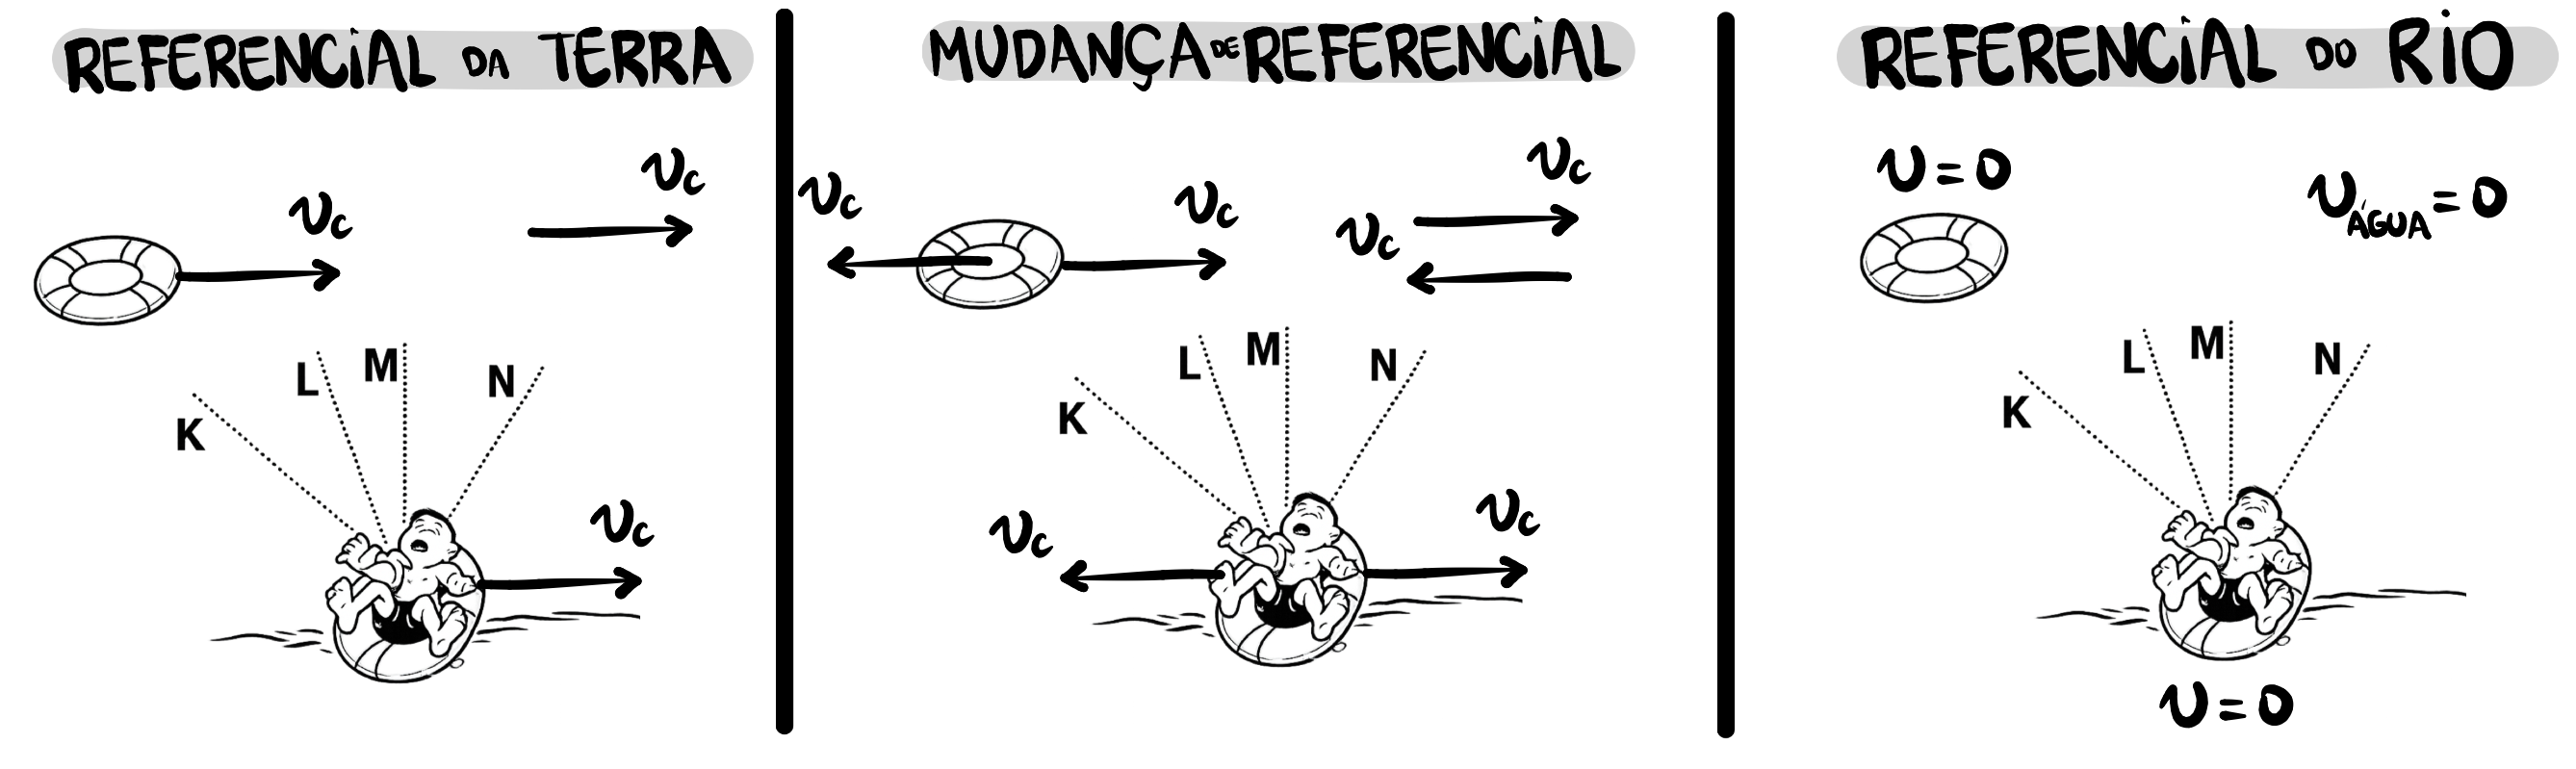
\includegraphics[width=1.0\linewidth]{imagensmecanica/imagem_sem_fundo_2.png}
\captionof{figure}{Mudando do referencial das margens (terra) para o referencial da água (rio).}
\label{fig_mec_ufmgboiarioexemplo02}
} 
\vspace{0.3cm}
A última imagem mostra o resultado: no referencial do rio todos os objetos estão em repouso: a velocidade do menino, da bóia e das águas é nula -- mas este problema já foi resolvido por nós: a direção na qual o menino deve nadar para pegar a bóia é a direção K. \\

Viu só como olhar o problema da perspectiva (referencial) correto muda tudo?


\end{exemplo}



\vspace{0.3cm}






% \begin{exemplo}[Nível III (ITA 2013)]\label{exemplo_cinematica_vrelativa03}

% Ao passar pelo ponto $O$, um helicóptero segue na direção norte com velocidade $v$ constante. Nesse momento, um avião passa pelo ponto $P$, a uma distância $\delta$ de $O$, e voa para o oeste, em direção a $O$, com velocidade $u$ também constante, conforme mostra a figura.

% {
% \centering
% 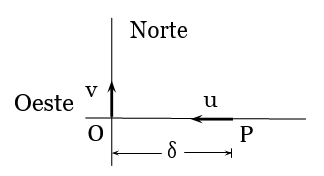
\includegraphics[width=0.3\linewidth]{imagensmecanica/vrelativaITA2013exemplo.png}
% \captionof{figure}{}
% \label{fig_mec_ita2013mudancareferencial}
% } 



% Considerando $t$ o instante em que a distância $d$ entre o helicóptero e o avião for mínima, assinale a alternativa correta.

% \begin{enumerate}
%   \item [(a)] A distância percorrida pelo helicóptero no instante em que o avião
%   alcança o ponto $O$ é $\delta u / v$.
  
%   \item [(b)] A distância do helicóptero ao ponto $O$ no instante $t$ é igual a
%   $\delta u / \sqrt{v^2 + u^2}$.
  
%   \item [(c)] A distância do avião ao ponto $O$ no instante $t$ é igual a
%   $\delta v^2 / (v^2 + u^2)$.
  
%   \item [(d)] O instante $t$ é igual a $\delta v / (v^2 + u^2)$.
  
%   \item [(e)] A distância $d$ é igual a $\delta u / \sqrt{v^2 + u^2}$.
% \end{enumerate}



% \resolucao


% Essa é uma questão cujo nível sobressai neste momento pelo fato de envolver um movimento bidimensional. A sua resolução, desse modo, talvez fique mais clara após o estudo da parte de Cinemática Vetorial. Contudo, a ideia principal é a mudança de referencial, de modo que pareceu oportuno trazê-la neste momento. \\

% Note que o problema é um pouco complicado porque temos dois objetos -- o avião e o helicóptero -- se movendo, e em direções distintas, inclusive. Note que o enunciado não especificou em relação a quem tais velocidades são medidas, de modo que assumimos que tais valores são relativos a um observador parado na terra. Vamos optar, por exemplo, por olhar o problema no referencial do avião -- isto é, o referencial no qual o avião está parado.  \\

% Desse modo, para pará-lo e fazer a mudança de referencial Terra $\to$ Avião, adicionamos a velocidade $u$ para direita a todos os corpos do sistema, como mostra a primeira imagem da Figura \ref{fig_mec_mudancareferencialITA2d}. Isso fará com que o avião esteja parado -- é o que queríamos -- e que a velocidade resultante do helicóptero, neste referencial, seja dada pela soma vetorial das velocidades $v$ e $u$, o que aparece na segunda imagem da figura. Tal velocidade pode ser obtido pelo Teorema de Pitágoras, sendo dado por $w=\sqrt{v^2+u^2.}$

% {
% \centering
% 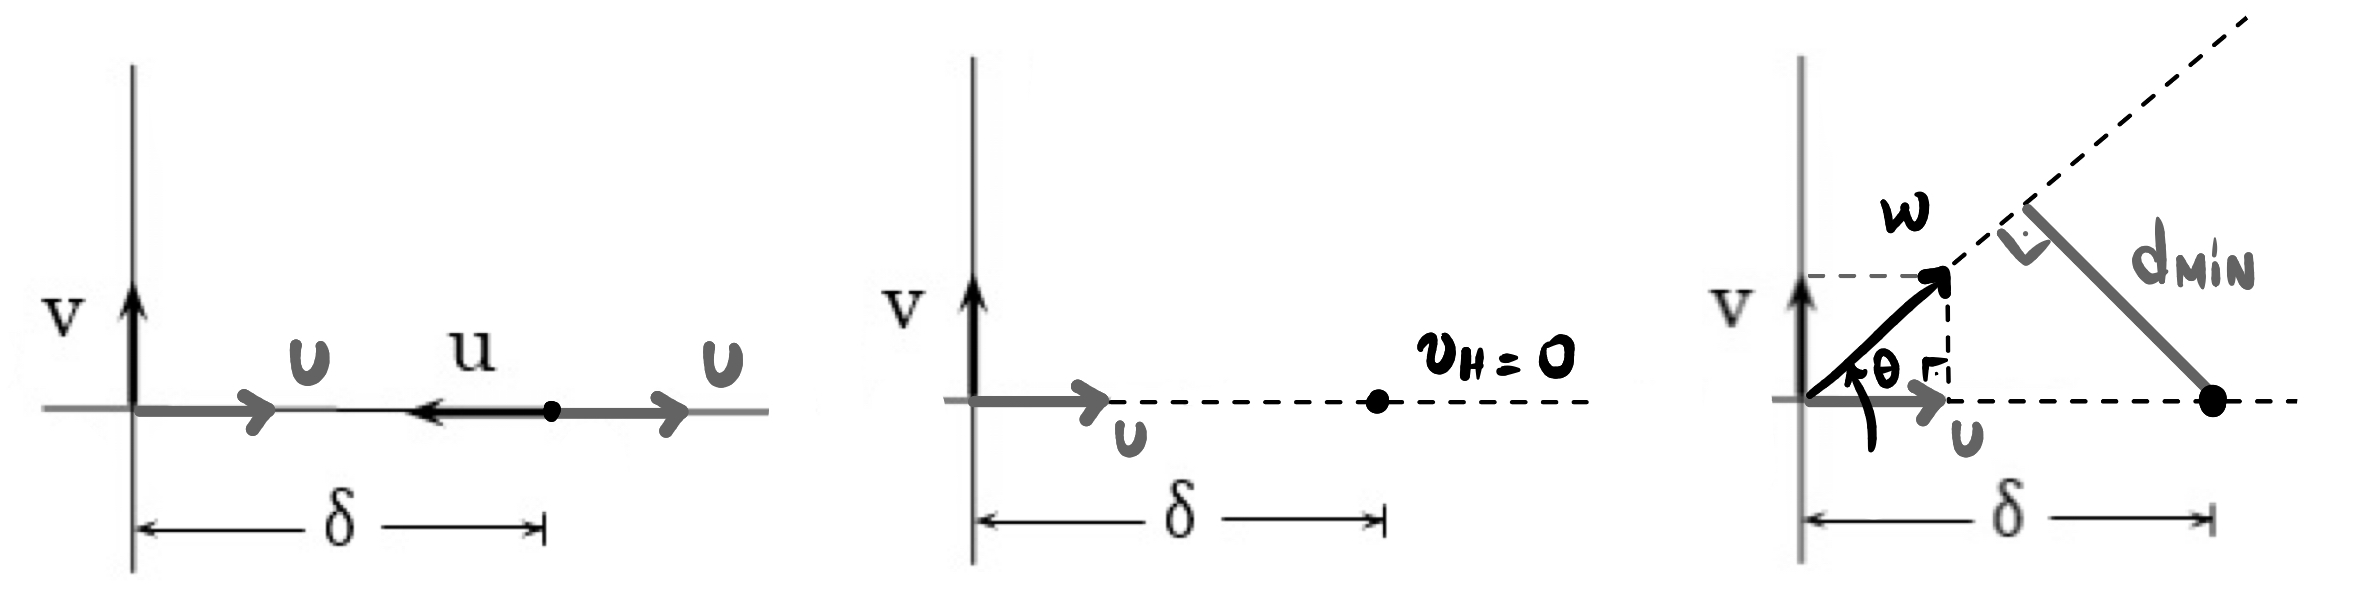
\includegraphics[width=0.80\linewidth]{imagensmecanica/mudancareferencialITA2d.jpeg}
% \captionof{figure}{}
% \label{fig_mec_mudancareferencialITA2d}
% } 


% A terceira imagem da figura mostra a trajetória do helicóptero no referencial do avião -- uma linha reta, inclinada de ângulo $\theta$ em relação à horizontal, sendo percorrida com velocidade $w$. Ora, no referencial do avião ele está parado, logo, a menor distância entre ele e o helicóptero será a menor distância entre um ponto e uma reta -- aquela tomada perpendicular à reta, destacada na terceira imagem da Figura \ref{fig_mec_mudancareferencialITA2d}. \\

% Podemos obter uma relação do $\sin \theta$ pelo trângulo dos vetores velocidade e o triângulo das distâncias, que fornecem, respectivamente:

% $$ \sin \theta =\dfrac{v}{w}= \dfrac{d_{min}}{\delta} \implies \boxed{d_{min}= \dfrac{ \delta v}{\sqrt{v^2+u^2}}.}$$

% Note que a distância entre dois pontos é uma propriedade geométrica invariante, ou seja, não depende do referencial -- a distância da ponta dos seus pés à sua cabeça é a sua altura, e este valor é o mesmo independente do referencial que o mede. Logo, a distância mínima entre os corpos obtida acima é uma grandeza absoluta, sendo, portanto, a mesma distância mínima que se obteria no referencial da terra. Com isso, eliminamos a alternativa E, que fornece o valor errado para tal distância. Vamos testar o que afirmam as outras alternativas:

% \begin{enumerate}
% \item [(a)] Para alcançar o ponto $O$ o avião leva um tempo $t'=\sfrac{\delta}{u},$ e, ao longo deste tempo, o helicóptero percorre uma distância dada por

% $$ d = vt'=  \dfrac{\delta v}{u},$$

% \noindent de modo que a alternativa $(a)$ também está errada.

%     \item [(b)] O tempo que demora até que se alcance a configuração em que a distância é mínima -- a situação da terceira imagem da Figura \ref{fig_mec_mudancareferencialITA2d} -- pode ser obtido fazendo a razão entre a distância percorrida pelo helicóptero neste referencial pela sua velocidade $w$ relativa ao mesmo referencial. A distância percorrida $x$ pode ser obtida por meio do $\cos \theta, $ pelo triângulo dos vetores velocidade e o trângulo de distâncias:

%     $$\cos \theta = \dfrac{u}{w} = \dfrac{x}{\delta} \implies x = \dfrac{\delta u}{\sqrt{v^2+u^2}},$$

%     \noindent de modo que o tempo para que isso ocorra é dado por 

%     $$ t = \dfrac{x}{w}=\dfrac{\delta u}{v^2+u^2},$$

%     \noindent de onde vemos que a letra $(d)$ está errada. Além disso, a distância do helicóptero ao ponto $O$ em tal instante é simplesmente

%     $$ d=vt= \dfrac{\delta uv}{v^2+u^2},$$

%     \noindent assim, a letra $(b)$ está errada.
    
    
%     Já a distância do avião ao ponto $O$ neste instante -- retornando ao referencial da terra -- é simplesmente dada por $(\delta - ut),$ haja vista que o helicóptero começa distando $\delta$ de tal ponto e se move com velocidade $u,$ no referencial da terra, em relação a ele. Logo, temos:

%     $$ \delta - ut = \delta - u\cdot \dfrac{\delta u}{v^2+u^2} = \dfrac{\delta v^2}{v^2+u^2},$$

%     \noindent de modo que a letra $(c)$ é a correta.



    
% \end{enumerate}


% \end{exemplo}



% \vspace{0.3cm}






\begin{exemplo}[Nível III (ITA 2009)]\label{exemplo_cinematica_vrelativa03}

Um barco leva 10 horas para subir e 4 horas para descer um mesmo trecho do rio Amazonas, mantendo constante o módulo de sua velocidade em relação à água. Quanto tempo o barco leva para descer esse trecho com os motores desligados?

\begin{enumerate}
    \item [a)] 14 horas e 30 minutos
    \item [b)] 13 horas e 20 minutos
    \item [c)] 7 horas e 20 minutos
    \item [d)] 10 horas
    \item [e)] Não é possível resolver porque não foi dada a distância percorrida pelo barco.
\end{enumerate}

\resolucao

Sejam $v$ o módulo da velocidade do barco em relação à água, $u$ o módulo da velocidade da correnteza e $d$ a extensão do trecho. Perceba que, com os motores desligados, o barco é carregado pela correnteza: sua velocidade em relação à margem é simplesmente $u$. Portanto, não precisamos encontrar $v$ nem $d$ separadamente — basta encontrar $u$.

Na subida, barco e correnteza se opõem, de modo que a velocidade resultante em relação à margem é $v - u$. Na descida com motores ligados, ambos cooperam, resultando em $v + u$. Usando $v=d/t$ em cada trecho:

$$v - u = \dfrac{d}{10}, \qquad v + u = \dfrac{d}{4}.$$

Subtraindo a primeira equação da segunda, eliminamos $v$:

$$2u = \dfrac{d}{4} - \dfrac{d}{10} = \dfrac{5d - 2d}{20} = \dfrac{3d}{20} \implies u = \dfrac{3d}{40}.$$

Com os motores desligados, o barco desce o trecho $d$ à velocidade $u$:

$$\Delta t = \dfrac{d}{u} = \dfrac{d}{\dfrac{3d}{40}} = \dfrac{40}{3} \text{ h} = \dfrac{39}{3} \text{ h} + \dfrac{1}{3} \text{ h}= 13\text{ h } 20\text{ min} \implies \text{letra B.}$$



\end{exemplo}

\vspace{0.3cm}



  











\begin{secnivel}[Aceleração Escalar Média]{I}{Aceleração Escalar Média}
  
  \eqLdois{def}{mecanica_eq_aceleracaomedia}{a_m := \dfrac{\Delta v}{\Delta t} }

\end{secnivel}
  






\secgfe{De onde vem}
O conceito de aceleração é criado a partir da necessidade de mensurar o quão rápido um movimento varia. Observe a situação Figura \ref{fig_mec_aceleracao01}. 

\begin{figure}[h]
    \centering
    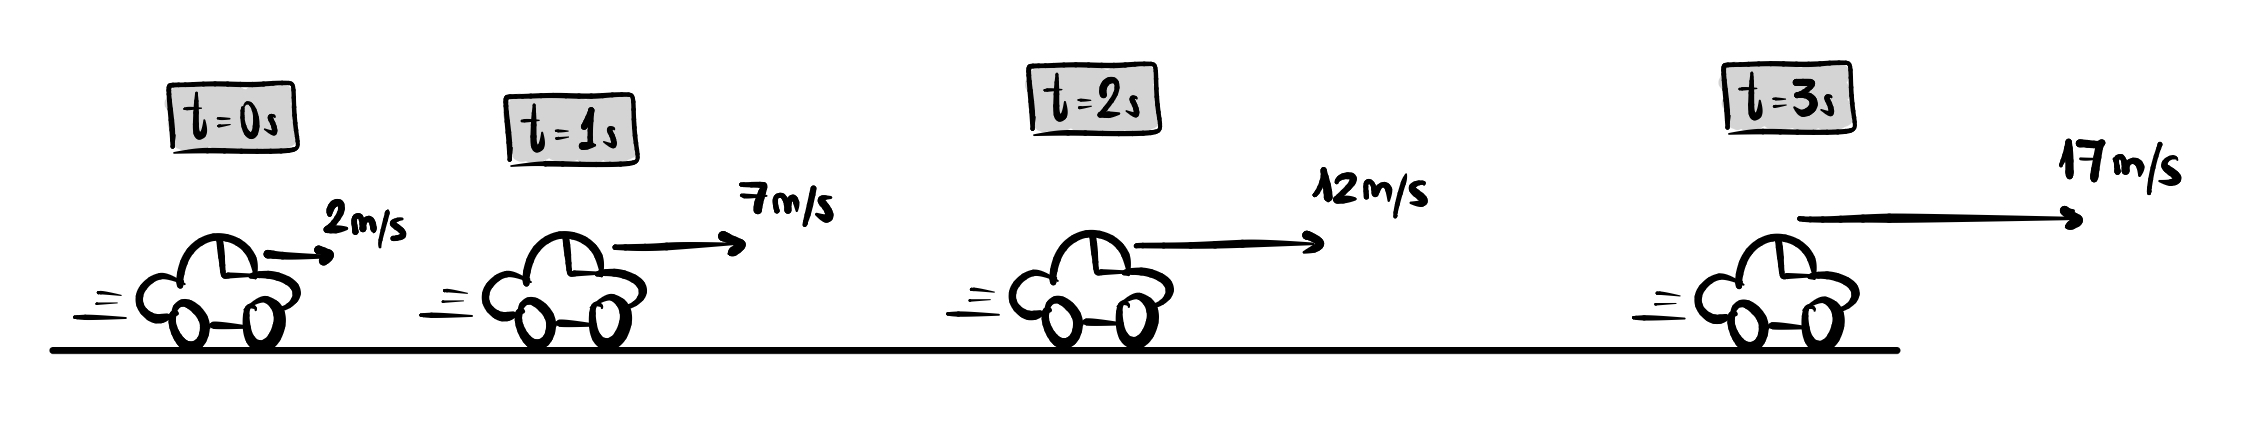
\includegraphics[scale=0.18]{imagensmecanica/acelerecao01.jpeg}
    \caption{Carro em movimento acelerado.}
    \label{fig_mec_aceleracao01}
\end{figure}



Como poderíamos comunicar a alguém acerca do que estamos vendo? Poderíamos dizer que estamos vendo um carro que anda cada vez mais depressa, com sua velocidade aumentando. Mas o quão mais depressa esse carro se move? Como essa velocidade aumenta?



%Poderíamos, é claro, simplesmente descrever o que vemos na figura: no instante inicial o carro possui velocidade de $2$ m/s; no instante $t=1s$ a sua velocidade é de $5$ m/s; no instante $t=2s$ a sua velocidade é de $12$ m/s e em $t=3s$ a sua velocidade é de $17$ m/s.



Para responder perguntas como essa é que estendemos o nosso vocabulário, introduzindo o conceito de aceleração, que irá medir justamente o quão rápido a velocidade está mudando à medida que tempo passa. Avaliando melhor o contexto, vemos, como mostra a Figura \ref{fig_mec_aceleracao02}, que há uma certa regularidade na forma como a velocidade varia: ela varia de exatamente $5$ m/s a cada segundo que passa, e a isso damos o nome de aceleração. Poderíamos dizer que o carro tem uma aceleração de $5$ m/s por segundo, ou seja, sua velocidade varia de $5$ m/s a cada segundo. Mas é mais comum dizermos que sua aceleração é de $5$ metros por segundo ao quadrado, ou $5\text{ m}/\text{s}^2,$ como pode ser destrinchado matematicamente:

$$ a = \dfrac{\Delta v}{\Delta t} = \dfrac{5\text{ m}/\text{s}}{1 \text{s}} = 5\text{ m}/\text{s}^2. $$



\begin{figure}[h]
    \centering
    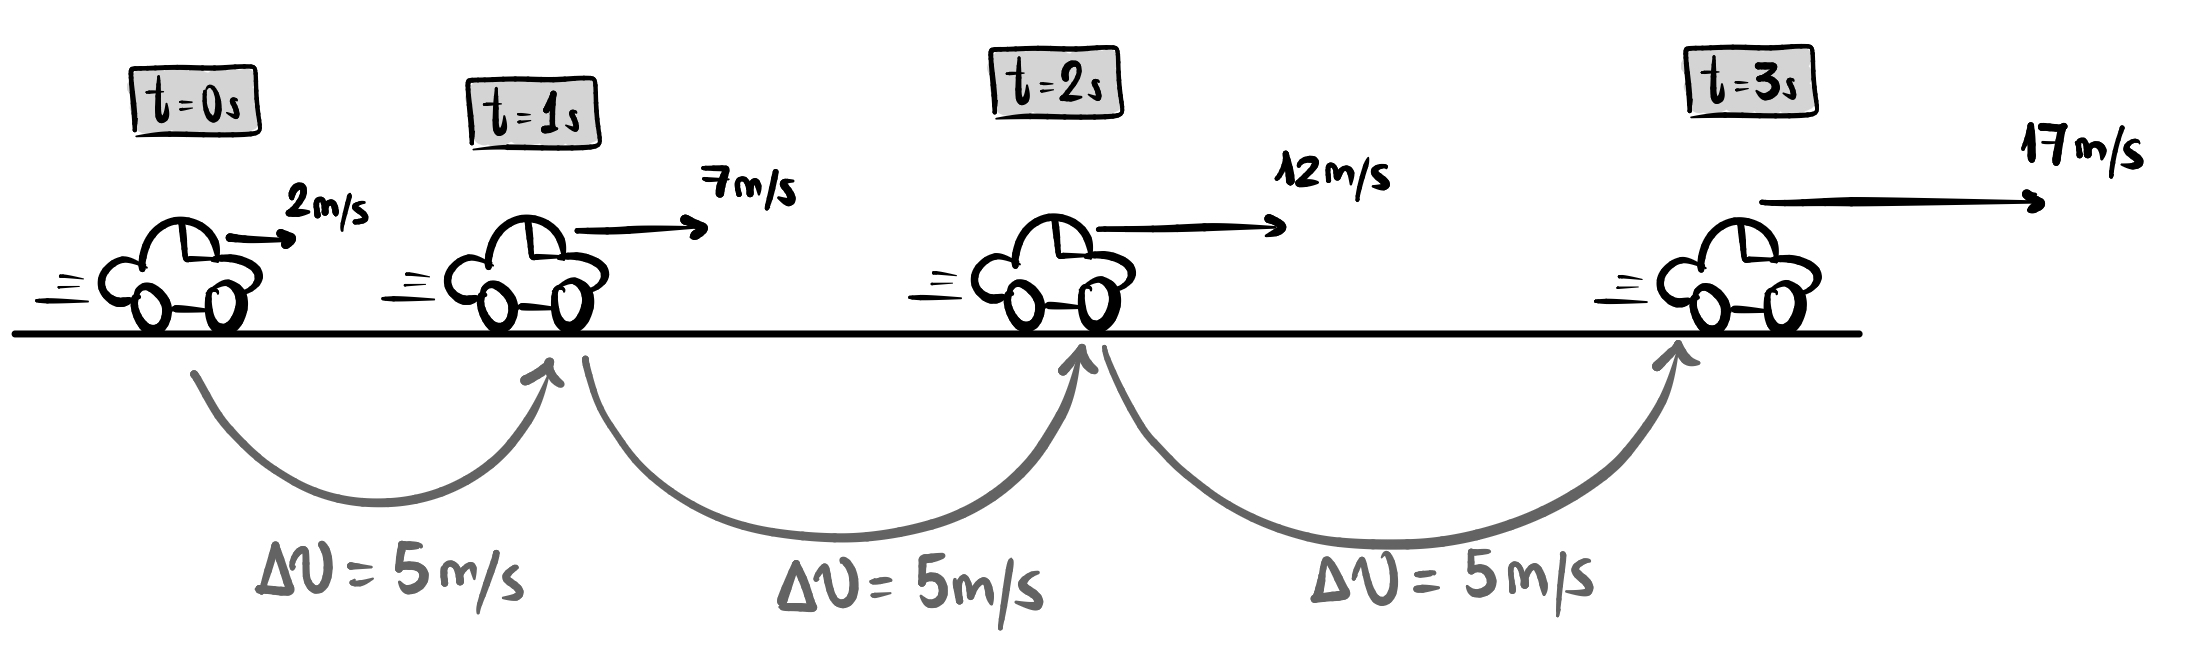
\includegraphics[scale=0.18]{imagensmecanica/acelerecao02.jpeg}
    \caption{Carro em movimento acelerado e o padrão de aumento de velocidade}
    \label{fig_mec_aceleracao02}
\end{figure}

Agora, munidos de tal conceito, temos mais vocabulário para estudar o movimento dos corpos -- em particular, corpos que se movem com velocidade variável.


\secgfe{Onde é usada}

Pode ser usada como uma aplicação direta para computar a aceleração de algum objeto que esteja se movendo. Por se tratar de uma equação que tem a ver com movimento -- ela mede o quão rápido o movimento (a velocidade) está mudando à medida que o tempo passa -- a aceleração irá aparecer em diversas fórmulas, como todas as de Cinemática, relativas ao movimento com aceleração constante, como:

$$ \Delta s = v_0t + \dfrac{1}{2}at^2 \quad ; \quad v^2 = v_0^2 + 2a\Delta s.$$

Além disso, como veremos futuramente, as forças são o que causam a aceleração dos corpos, de modo que a aceleração aparece na Segunda Lei de Newton:

$$ F = ma.$$


\secgfe{Erros comuns}

O erro mais comum certamente é confundir velocidade com aceleração. Para que fique bem claro: a velocidade mede o quão rápido um corpo de move, já a aceleração mede o quão rápido varia a velocidade desse mesmo corpo.

Desse modo, um corpo pode ter aceleração zero e ainda estar se movendo: se a aceleração é zero, significa que sua velocidade não varia, logo, tal corpo deve, necessariamente, estar se movendo com velocidade constante.

Portanto, atenção: se um corpo está em movimento ele \textbf{não precisa ter aceleração.} Se ele estiver em um movimento em que sua velocidade varia, aí sim ele precisa, \textbf{necessariamente}, ter aceleração.



\secgfe{Observações}

No Sistema Internacional de Unidades de Medida (SI) a unidade padrão para medir velocidade é o $\text{ m}/\text{s}$, e a unidade padrão para medida de tempo é o segundo, $\text{s}.$ Desse modo, a unidade padrão no (SI) para medir aceleração é, consequentemente, o $\text{ m}/\text{s}^2$.


É claro que alguém poderia medir a velocidade em $\text{km}/\text{h},$ o tempo em segundos, e computar uma aceleração medida em $\sfrac{\text{km/h}}{\text{s}}$, isso só seria muito estranho e bem pouco usual de ser feito.

\vspace{0.3cm}

\begin{exemplo}[Nível I]\label{exemplo_cinematicaescalar_aceleracaomedia01}


Considere um objeto, abandonado do repouso, a uma certa altura. Percebe-se que no terceiro segundo de seu movimento sua velocidade é de $12$ m/s. Já no quinto segundo do seu movimento sua velocidade é de $20$ m/s. Qual é a aceleração que tal objeto experimenta ao longo de seu movimento?



\resolucao



Usando a definição, e os valores de velocidade em $t_3=3$s e $t_5=5$s, temos que a aceleração média do objeto nestes 2 segundos de movimento foi

$$ a = \dfrac{\Delta v}{\Delta t} = \dfrac{v_5-v_3}{t_5-t_3}=\dfrac{20-12}{5-3} = \dfrac{8 \text{ m/s}}{2 \text{ s}} = 4 \text{m/s}^2.$$

  

    
\end{exemplo}

\vspace{0.3cm}




\begin{exemplo}[Nível II]\label{exemplo_cinematicaescalar_aceleracaomedia02}



Uma partícula move-se ao longo de uma trajetória retilínea orientada. Seu movimento ocorre em três intervalos de tempo consecutivos, de durações $\Delta t$, $2\Delta t$ e $3\Delta t$, respectivamente. As velocidades da partícula nos instantes inicial e final de cada intervalo são dadas a seguir:

\begin{itemize}
  \item [(i)] no instante inicial do primeiro intervalo, a velocidade vale $v$;
  \item [(ii)] no instante final do primeiro intervalo, a velocidade vale $2v$;
  \item [(iii)] no instante final do segundo intervalo, a velocidade vale $-v$;
  \item [(iv)] no instante final do terceiro intervalo, a velocidade vale $v$.
\end{itemize}

Não se dispõe de nenhuma outra informação sobre como a velocidade varia no interior de cada intervalo. Encontre a aceleração média da partícula durante o intervalo total de tempo.



\resolucao



Note que, para computar a aceleração média em um intervalo de tempo qualquer, tudo que precisamos é da velocidade $v_f$ no final de tal intervalo e da velocidade $v_0$ no início de tal intervalo. Toda e qualquer informação sobre velocidade durante tal intervalo é, portanto, irrelevante. \\

No caso do problema, as únicas informações importantes são aquelas dos itens $(i)$ e $(iv)$ -- a velocidade inicial no início de todo o movimento e a velocidade final no final do último trecho -- todo o resto é distração. Assim, ao longo de todo o trecho de duração $\Delta t+ 2\Delta t+3\Delta t = 6\Delta t$, a aceleração média é

$$ a_m = \dfrac{\Delta v}{\Delta t} = \dfrac{v_f-v_0}{6 \Delta t} = \dfrac{v-v}{6 \Delta t} = 0.$$

  

    
\end{exemplo}



\vspace{0.3cm}






















\newpage





\section{Movimento Uniforme}

O Movimento Uniforme (MU) é aquele no qual a velocidade possui valor constante. Observe, por exemplo, a Figura \ref{fig_mec_mu01}, que mostra um movimento uniforme unidimensional: o tempo passa e o valor de velocidade é sempre exatamente o mesmo (4 m/s, neste caso). Isso é o que caracteriza um movimento uniforme: o corpo percorre distâncias iguais em intervalos de tempos iguais, ou, caso o leitor prefira, a distância percorrida é sempre diretamente proporcional ao tempo transcorrido.


\begin{figure}[h]
    \centering
    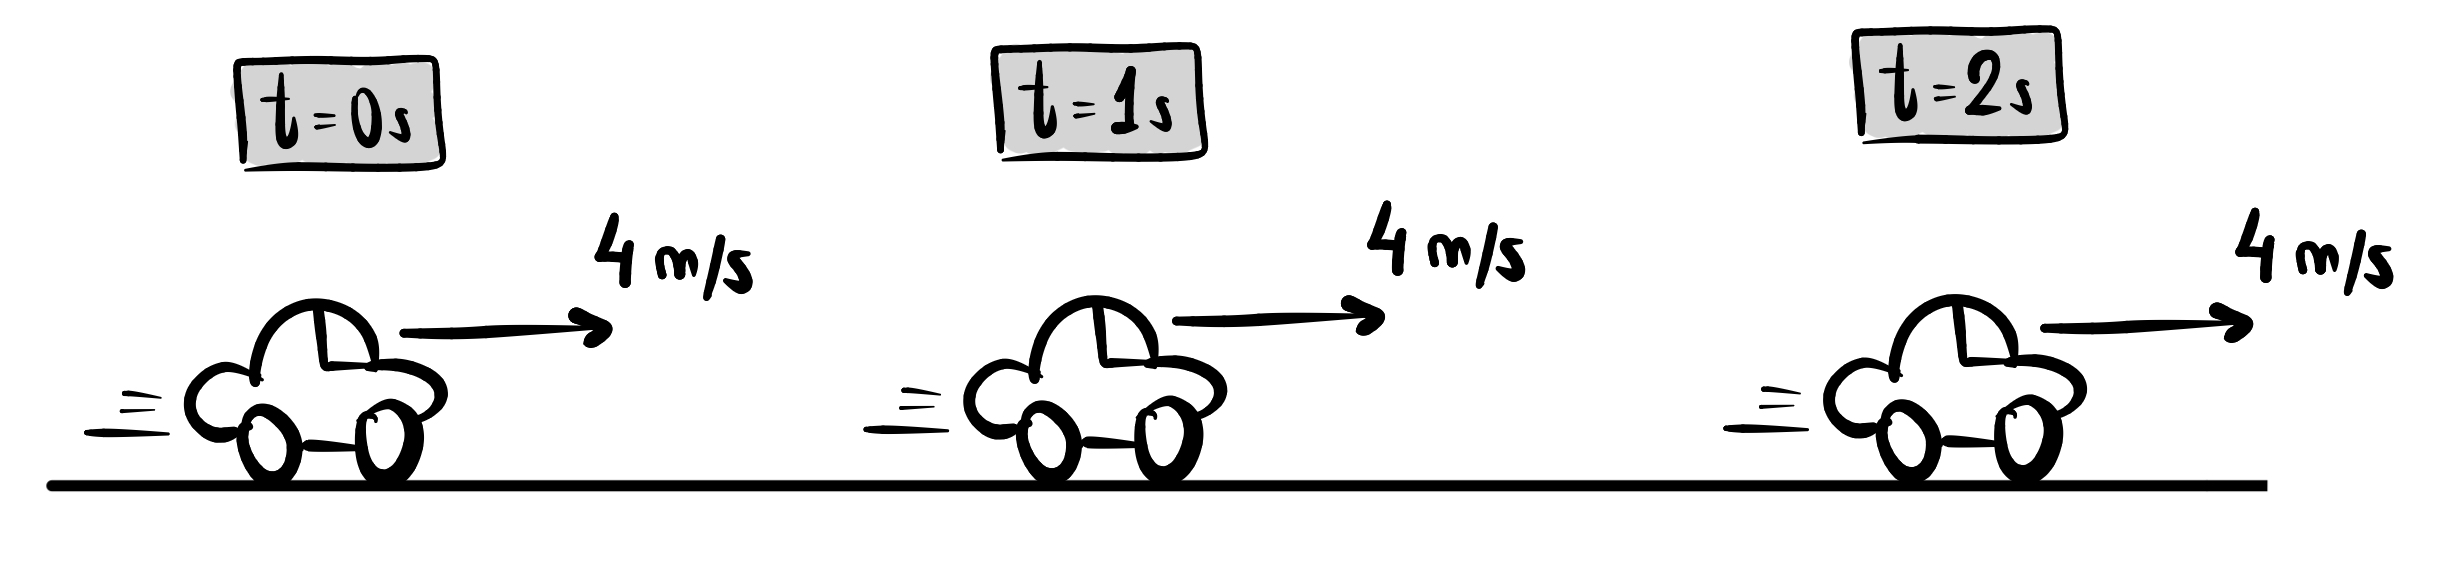
\includegraphics[scale=0.12]{imagensmecanica/mu01.jpeg}
    \caption{O Movimento Uniforme.}
    \label{fig_mec_mu01}
\end{figure}

Note, contudo, que o caso da Figura \ref{fig_mec_mu02} não constitui um MU, como talvez alguém poderia pensar, haja vista que o valor da velocidade é sempre de $4$ m/s. Não se trata de um MU, e vamos destacar dois aspectos que evidenciam isso:

\begin{itemize}
    \item [(i)] Note que, para que se alcance o cenário em $t=2$s, seria preciso que a velocidade do carro, a partir de $t=1s$, fosse diminuindo, até zerar. A partir deste momento o carro conseguiria inverter o sentido do seu movimento, começando a acelerar no sentido oposto, aumentando o valor de sua velocidade até alcançar o valor de $4$ m/s.

    Ou seja, o movimento foi acelerado entre $t=1$s e $t=2$s: a velocidade não ficou constante, de modo que não se trata de um MU.


    \item [(ii)] Dada a discussão do tópico anterior, está claro como que uma velocidade de $4$ m/s apontando para a direita é diferente de uma velocidade de $4$ m/s apontando para a esquerda -- e que deve haver aceleração para sair de uma configuração para outra.

    Dito isso, como faremos para não confundir essas duas situações? A Figura \ref{fig_mec_mu02} deixa isso claro: ao adotar um eixo de referência para marcar posições (um referencial), imediatamente isso já define um sentido positivo -- o sentido no qual as posições crescem -- e um sentido negativo -- o sentido no qual as posições diminuem.\footnote{Caso o leitor não tenha se dado conta de que isso é imediato, perceba que trata-se apenas de uma consequência da forma como definimos a velocidade. Considere as posições $10$m e $12$m, e um MU entre as duas que dura $1$s. Um corpo que sai de $s_0=10$m para $s_f=12$m terá velocidade média dada por $\sfrac{\Delta s}{\Delta t}=\sfrac{(12-10)}{1}=+2\text{m/s}$; já um corpo que sai de $s_0=12$m para $s_f=10$m terá velocidade média dada por $\sfrac{\Delta s}{\Delta t}=\sfrac{(10-12)}{1}=-2\text{m/s}$. Ou seja, quando nos movemos no sentido em que as posições diminuem a velocidade automaticamente já aparece com sinal negativo no cálculo -- o contrário também sendo verdadeiro. Logo, o fato da velocidade positiva ser aquela que aponta no sentido crescente das posições e a velocidade negativa ser aquela que aponta no sentido decrescente das posições é apenas uma consequência de como a velocidade média é definida, e não um fato extra que inserimos artificialmente na teoria. Esses dois movimentos, inclusive, recebem nomes: movimento progressivo -- quando a velocidade é positiva, ou seja, o corpo progride no eixo das posições -- e movimento retrógrado -- quando a velocidade é negativa, ou seja, o corpo retrocede no eixo das posições. } Desse modo, uma velocidade que aponte para a direita será considerada positiva, enquanto uma velocidade que aponta para a esquerda será considerada negativa. Assim, podemos diferenciar as duas situações, e fica claro que $+4$ m/s indica uma velocidade para a direita enquanto que $-4$ m/s indica uma velocidade para a esquerda.

    Isso também vale para acelerações -- uma aceleração negativa quer dizer simplesmente que ela aponta para o sentido contrário em que as posições crescem. Dito isso, é importante ressaltar: \textbf{o sinal de grandezas como velocidade e aceleração na cinemática está relacionado unicamente ao sentido no qual tais grandezas apontam, e é usado, justamente, para diferenciar corpos que se movem em sentidos opostos ao longo de uma mesma direção.}\footnote{Vale lembrar que o sentido em que as coisas crescem é arbitrário -- depende da escolha que se faça.}
\end{itemize}





\begin{figure}[h]
    \centering
    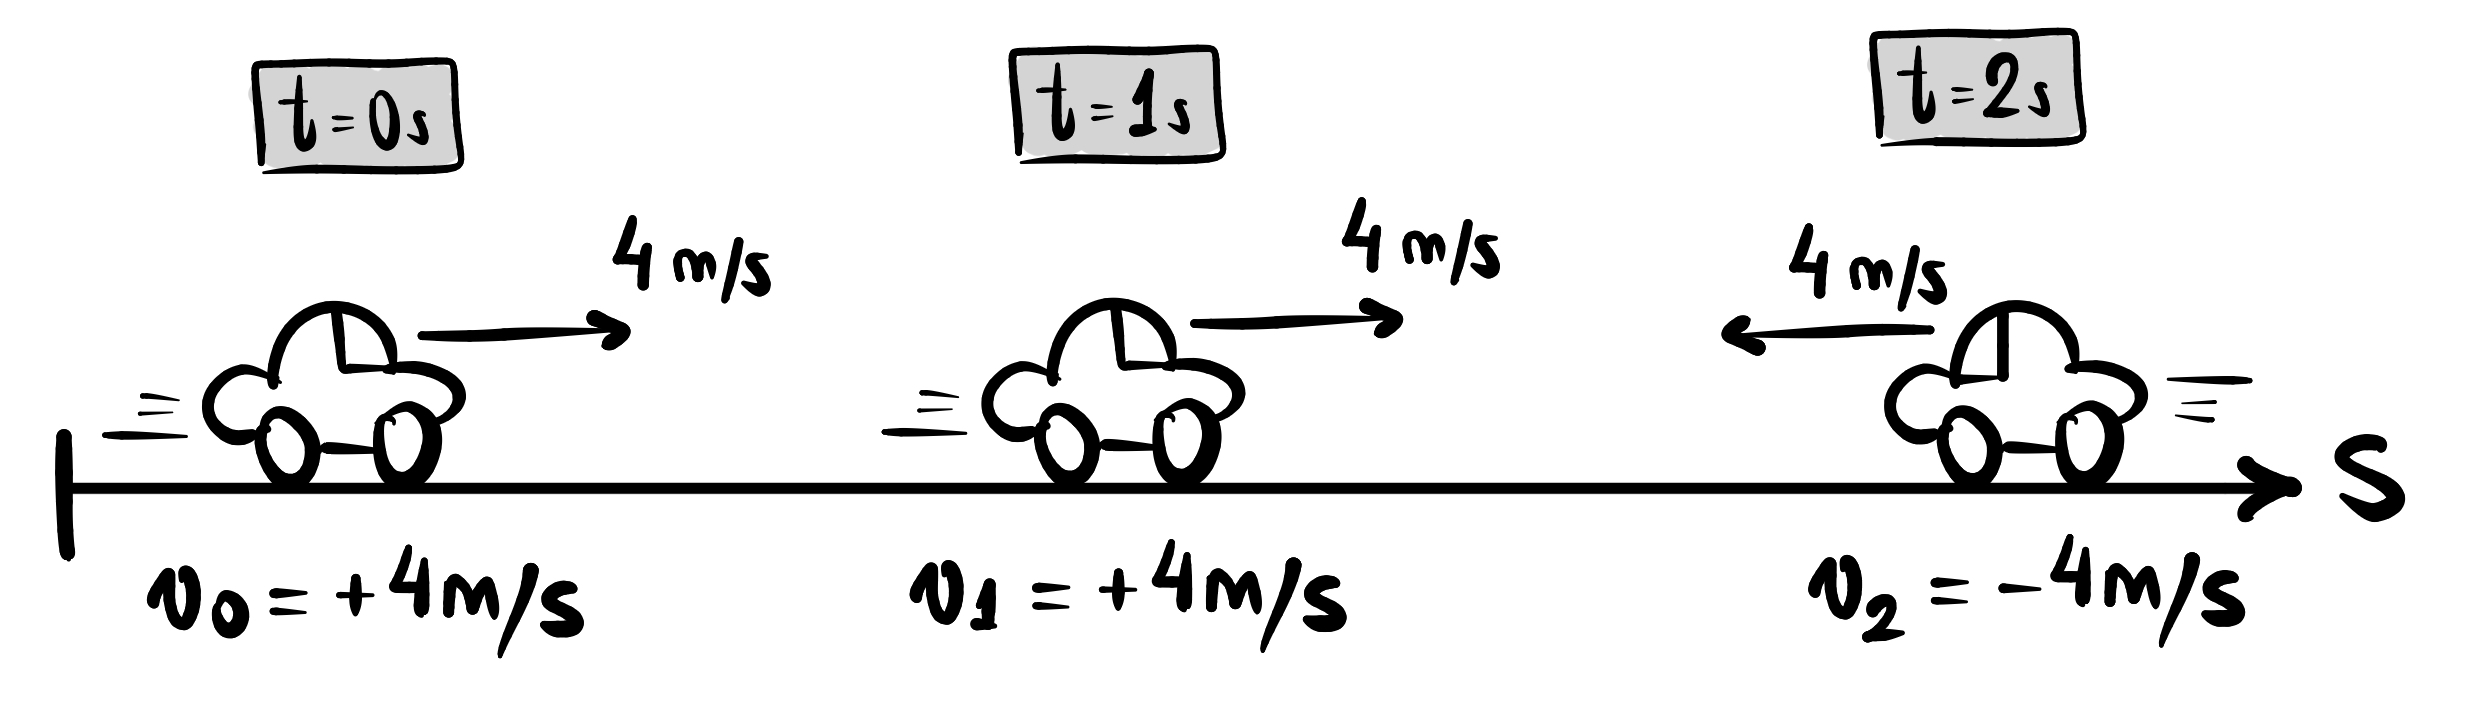
\includegraphics[scale=0.12]{imagensmecanica/mu02.jpeg}
    \caption{O sinal de uma grandeza física como velocidade ou aceleração está relacionado ao sentido em que tal grandeza aponta.}
    \label{fig_mec_mu02}
\end{figure}



\begin{secnivel}[Distância no Movimento Uniforme]{I}{Distância no Movimento Uniforme}
 

  \eqLdois{dem}{mecanica_eq_distanciamu}{d=vt}
  
\end{secnivel}







\secgfe{De onde vem}

Essa talvez seja a equação mais básica de toda a Física, e serve para calcular a distância percorrida por um corpo que executa um Movimento Uniforme.

Ela é uma consequência imediata da definição de velocidade média, feita na Equação \eqref{mecanica_eq_velocidademedia}. Note que, se temos um MU, isso significa que a velocidade é constante o tempo inteiro, por definição. Isso quer dizer, consequentemente, que o sentido do movimento nunca muda, isto é, se o corpo se move inicialmente para a direita, como mostra Figura \ref{fig_mec_mu01}, ele irá se mover para direita ao longo de todo o movimento -- caso contrário, para inverter o sentido do movimento, o corpo teria que acelerar, como vimos na situação da Figura \ref{fig_mec_mu02}, de modo que isso descaracterizaria o MU.

Dito isso, cabe ao leitor lembrar da nossa discussão feita na definição da Equação \eqref{mecanica_eq_velocidademedia} sobre a diferença entre o deslocamento $\Delta s$ e a distância percorrida $d$. Deixamos claro que essas duas grandezas deixam de coincidir quando há inversão no sentido do movimento. Logo, no MU, como isso nunca ocorre, distância e deslocamento sempre coincidirão, de modo que, a partir da Equação \eqref{mecanica_eq_velocidademedia}, podemos escrever

$$ v_m = \dfrac{\Delta s}{\Delta t} = \dfrac{d}{t-0} \implies v_m = \dfrac{d}{t},$$

\noindent em que escolhemos o instante inicial do movimento como sendo $t_0=0.$ Ora, como a velocidade no MU é constante, a velocidade média, $v_m$, em qualquer intervalo de tempo analisado irá sempre coincidir com a velocidade, $v$, do carro -- que é sempre a mesma. Logo, $v_m=v,$ de modo que a equação acima se torna

$$ v_m=v=\dfrac{d}{t} \implies \boxed{ d=vt,}$$

\noindent e está provado que, no MU, a distância é igual ao produto da velocidade pelo tempo. É importante que o leitor note que o argumento principal para que isso funcionasse estava pautado em dois critérios:

\begin{itemize}
    \item [(i)] O deslocamento $\Delta s$ e a distância percorrida $d$ coincidem para um corpo que executa um Movimento Uniforme, isto é:

    $$\Delta s = d.$$

    \item [(ii)] A velocidade $v$ do corpo, no MU, é sempre exatamente a mesma, de modo que ela coincide com a velocidade média em qualquer intervalo de tempo que se analise, ou seja:

    $$ v_m = v.$$
\end{itemize}

Esses dois critérios serão sempre atendidos exclusivamente para o MU, de modo que a Equação \eqref{mecanica_eq_distanciamu} será válida apenas para um corpo que executa um MU.


\secgfe{Onde é usada}

Em problemas que envolvem corpos que se movam com velocidade constante.



\secgfe{Erros comuns}

Essa, como dito, é uma das equações mais simples da física, de modo que não deixa tanta margem para que se cometa muitos erros que não sejam erros simples de cálculos matemáticos.

Talvez o principal erro aqui seja o estudante acreditar que essa é a equação fundamental do movimento de toda a Física, ou seja, que ela vale para qualquer tipo de movimento. Isso está, claramente, errado, e fizemos questão de evidenciar que a Equação \eqref{mecanica_eq_distanciamu} vale apenas para um corpo que executa um Movimento Uniforme. Caso o leitor queira aplicar tal equação para calcular a distância percorrida por um carro que acelera, ou que desacelera, ou qualquer outro tipo de movimento que não seja o MU, a equação irá fornecer certamente valores errados, por não se aplicar em tais regimes.



\secgfe{Observações}

A observação mais relevante aqui talvez seja a de que, em muitos problemas, o uso direto da Equação \eqref{mecanica_eq_distanciamu} pode acabar sendo o caminho mais complicado para resolver o problema. Em muitos problemas de Cinemática que envolvem o MU, a situação é drasticamente simplificada caso, primeiro, usemos a Equação \eqref{mecanica_eq_velocidaderelativa} para escolher o referencial adequado e, só então, usemos a Equação \eqref{mecanica_eq_distanciamu}. Isso ficará claro em alguns exemplos que resolveremos a seguir.





\vspace{0.3cm}


\begin{exemplo}[Nível I]\label{exemplo_distanciamovuniforme01}

Um carro se move com velocidade constante de 20 m/s ao longo de uma rodovia, enquanto outro se move com velocidade constante de 30 m/s, em sentido oposto, ao longo da mesma rodovia.

Se os carros inicialmente estão separados por uma distância de 1.2 km, após quanto tempo eles irão passar um pelo outro?

\resolucao

Vamos resolver esse problema de duas formas, mudando apenas o referencial.

\begin{itemize}
    \item [(i)] Referencial da Terra.

    A Figura \ref{fig_mec_muexemplo01} mostra a situação, em que os carros $A$ e $B$ estão separados de $1200$m. Digamos que eles vão se encontrar no ponto $P$, que, naturalmente, estará mais próximo de onde estava inicialmente o carro $A$, uma vez que este se move com uma velocidade menor.

    Sejam $d_A$ e $d_B$ as distâncias que os carros $A$ e $B,$ respectivamente, devem percorrer até chegar ao ponto de encontro $P$. Ora, tais distâncias devem varrer, somadas, a distância de $1200$m que inicialmente os separava, como a figura evidencia. Ou seja, matematicamente:

    $$ d_A + d_B = 1200.$$

    Sendo os movimentos uniformes, podemos usar a Equação \eqref{mecanica_eq_distanciamu} para cada um deles, ou seja, $d_A=v_A\cdot t = 20t$ e $d_B=v_b \cdot t = 30t,$ que, na equação acima, fornece:\footnote{Talvez o leitor pode ter ficado com a dúvida se a velocidade do carro que anda em sentido contrário não deveria ter entrado com sinal negativo na equação. Vamos discutir isso, em mais detalhes, na seção sobre a Equação \eqref{mecanica_eq_mu_funcaoposicao}.}

    $$ 20t + 30 t = 1200 \implies 50t=1200 \implies \boxed{t=24 \text{ segundos.}}$$



 {
\centering
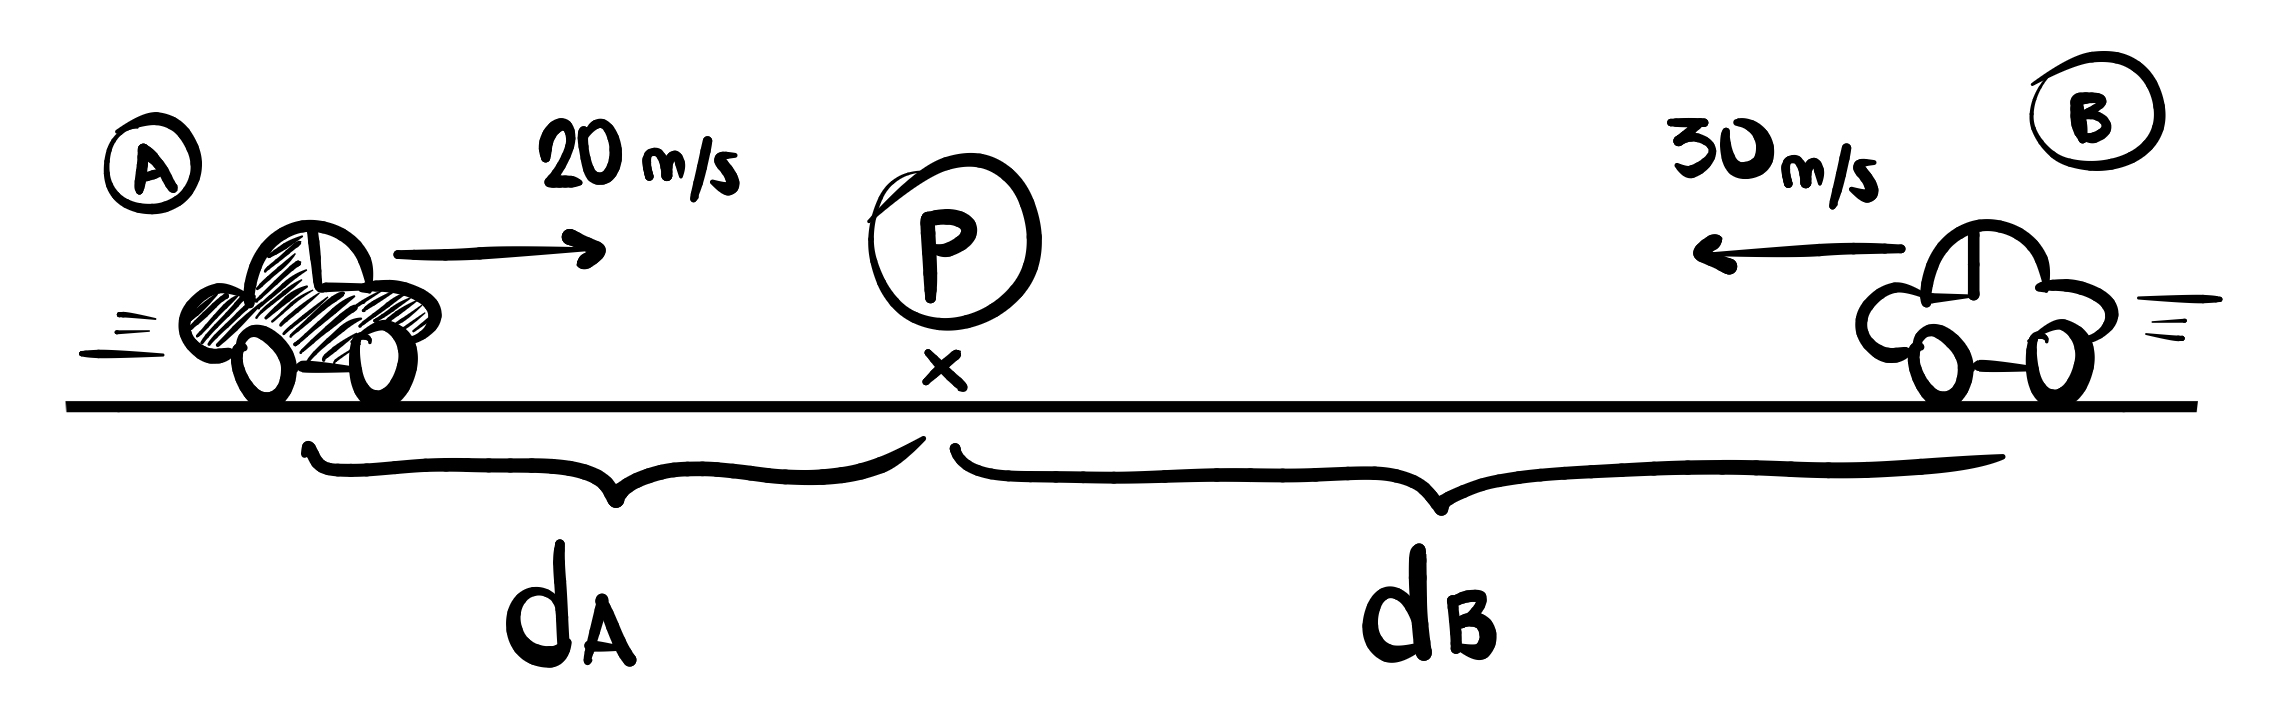
\includegraphics[width=0.6\linewidth]{imagensmecanica/muexemplo01.jpeg}
\captionof{figure}{}
\label{fig_mec_muexemplo01}
} 


    \item[(ii)] Referencial do carro $B$.

    Essa solução envolve fazer uma mudança de referencial, como aprendemos na construção da Equação \eqref{mecanica_eq_velocidaderelativa}. A Figura \ref{fig_mec_muexemplo0102} mostra, inicialmente, a situação no referencial da terra e, em seguida, a situação no referencial do carro $B.$ Lembrando que, para fazermos tal mudança, adiciona-se o oposto da velocidade de $B$ a todas as partículas do sistema, o que o faz ficar parado. Com isso, a velocidade do carro $A$ em relação ao carro $B$ é de $50$ m/s, como mostra a figura.


 {
\centering
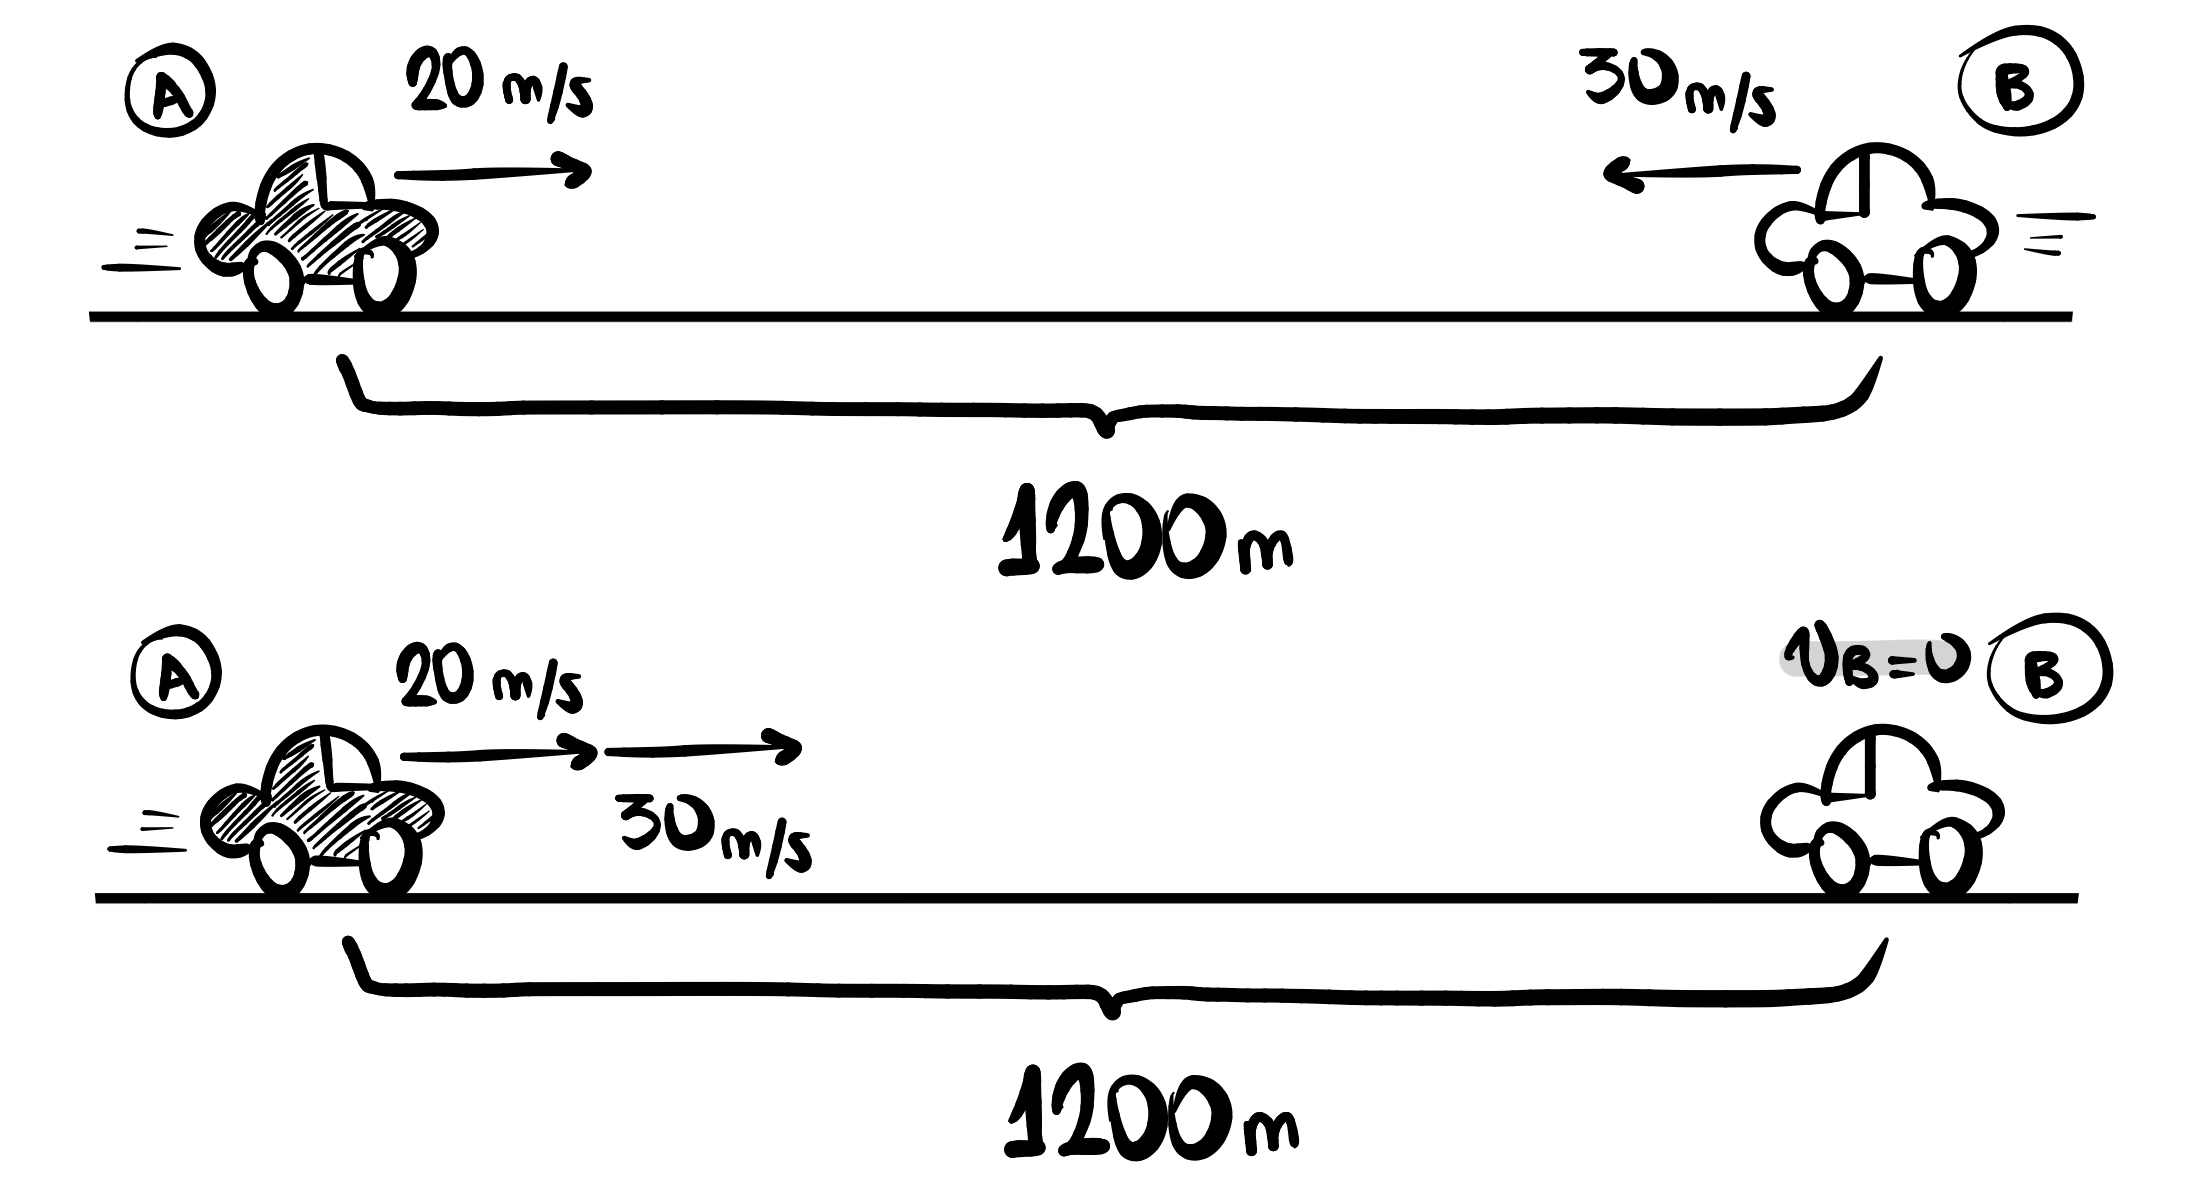
\includegraphics[width=0.6\linewidth]{imagensmecanica/muexemplo0102.jpeg}
\captionof{figure}{}
\label{fig_mec_muexemplo0102}
} 



Perceba que, agora, o problema ficou substancialmente mais simples: temos um carro que se move a $50$ m/s em direção a um outro carro, parado, que está afastado de $1200$m do primeiro. Sendo assim, o tempo que demora até que um carro encontre o outro é dado de forma direta por

$$ d = v \cdot t \implies 1200 = 50 t \implies \boxed{t = 24 \text{ segundos.}}$$

    
\end{itemize}

Note que, escolhendo o referencial adequado, o problema fica mais simples e, consequentemente, seus cálculos e sua resolução também. É sempre mais fácil resolver um problema de Cinemática em que há apenas um corpo em movimento e o outro fica parado. Quando os dois ou mais corpos se movem, a analise e os cálculos costumam ficar mais laboriosos -- é por isso que a mudança de referencial da segunda solução simplificou o problema. 


\end{exemplo}


\vspace{0.3cm}






\begin{exemplo}[Nível II]\label{exemplo_distanciamovuniforme02}


Dois trens partem, simultaneamente, um em direção ao outro, com velocidade constante de 80 km/h. O trem 1 sai da cidade A em direção à cidade B, enquanto o trem 2 sai da cidade B para a cidade A. A distância entre as cidades é de 640 km.

Uma mosca, inicialmente pousada na dianteira do trem 1, se move em direção à dianteira do trem 2. Ao chegar lá, ela imediatamente retorna até à dianteira do trem 1, e assim continua, até morrer esmagada pela colisão dos dois trens. Se a velocidade da mosca é de 120 km/h, qual é a distância total que ela percorre até ser esmagada?

\resolucao





Este problema, em um primeiro momento, pode parecer bastante complicado -- mas ele é bem parecido com o problema anterior. Note que a dificuldade parece residir no fato de que a mosca fica o tempo inteiro pulando de um lado para o outro -- isso enquanto os dois trens se aproximam um do outro, de modo que suas posições mudam e a mosca vai e volta cada hora até um lugar diferente.
\\

De fato é bem difícil avaliar o movimento da mosca. Contudo, isso não é necessário. Note que, a velocidade da mosca sendo constante, podemos usar que $d=v \cdot t.$ Como sabemos sua velocidade $v$, basta descobrirmos por quanto tempo $t$ ela ficará se movendo que será imediato obter a distância total $d$ que ela percorre. Ora, mas o tempo que ela se move é exatamente o tempo necessário para que os trens se encontrem, e isso é exatamente o que fizemos no problema anterior.

Mudando para o referencial de um dos trens, um ficará parado e o outro se moverá a uma velocidade de $80+80 = 160$ km/h, que, para varrer uma distância de $640$ km até colidir com o outro, levará um tempo de
$$ d= v \cdot t \implies 640 \text{ km} = 160 \text{ km/h} \cdot t \implies \boxed{t=4 \text{ h.}}$$

Assim, se a mosca se move por $4$ horas com uma velocidade de $120$ km/h, ela percorrerá, ao longo de todo o seu movimento, uma distância igual a

$$ d = vt = 120 \cdot 4 = \boxed{480 \text{ km.}}$$

\end{exemplo}


\vspace{0.3cm}






\begin{exemplo}[Nível III (ITA - 2007)]\label{exemplo_distanciamovuniforme03}


Considere que num tiro de revólver, a bala percorre trajetória retilínea com velocidade $v$ constante, desde o ponto inicial P até o alvo Q. 


 {
\centering
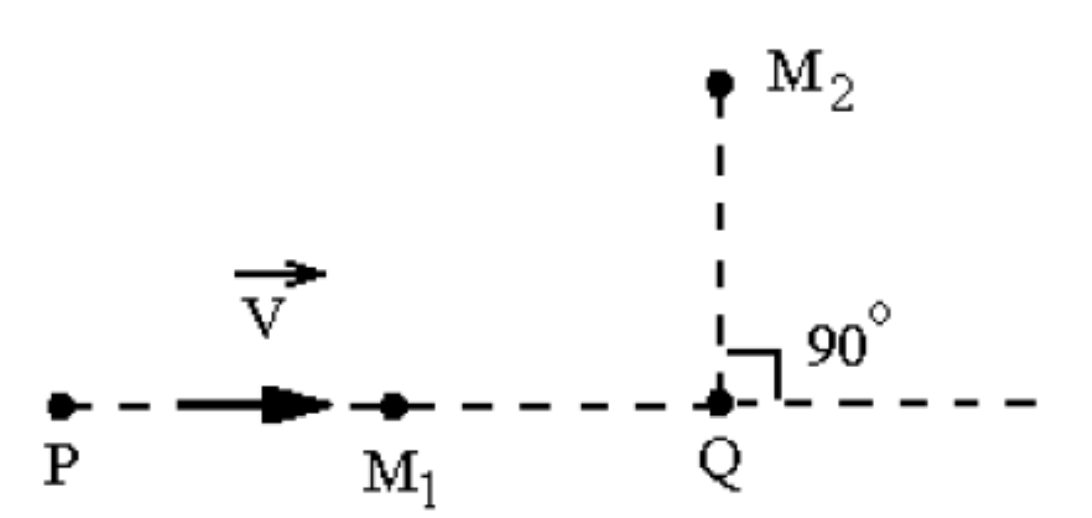
\includegraphics[width=0.35\linewidth]{imagensmecanica/muexemplo03ita.png}
\captionof{figure}{}
\label{fig_mec_muexemplo03ita2007}
} 



Mostrados na figura, o aparelho M$_1$ registra simultaneamente o sinal sonoro do disparo e o do impacto da bala no alvo, o mesmo ocorrendo com o aparelho M$_2$. Sendo $v_s$ a velocidade do som no ar, então a razão entre as respectivas distâncias dos aparelhos M$_1$ e M$_2$ em relação ao alvo
Q é

\begin{enumerate}
    \item [(a)] $\dfrac{v_s(v-v_s)}{v^2-v_s^2}$
    \item [(b)] $\dfrac{v_s(v_s-v)}{v^2-v_s^2}$
    \item [(c)] $\dfrac{v(v-v_s)}{v_2^2-v^2}$
    \item [(d)] $\dfrac{v_s(v\cdot v_s)}{v^2-v_s^2}$
    \item [(e)] $\dfrac{v_s(v-v_s)}{v^2\cdot v_s^2}$
\end{enumerate}

\resolucao


Considere as distâncias $x$, $y$ e $D$ nomeadas na Figura \ref{fig_mec_muexemplo03ita2007solution}. O que o enunciado nos pede é o valor da razão $\sfrac{x}{y}.$



 {
\centering
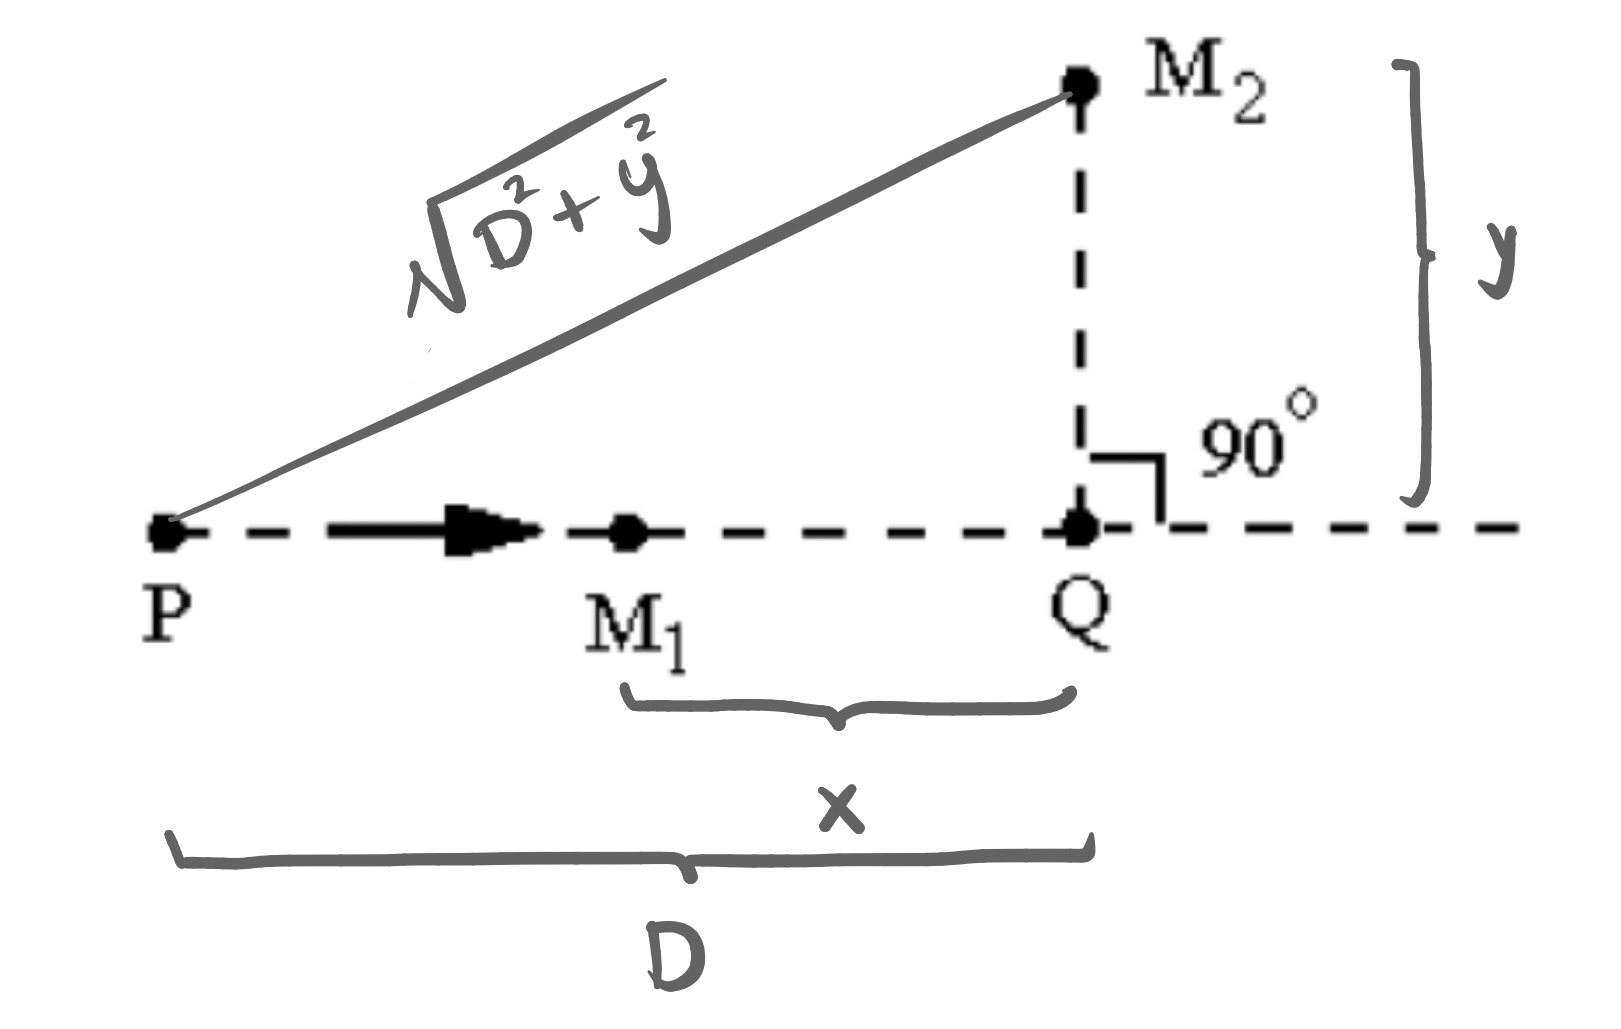
\includegraphics[width=0.4\linewidth]{imagensmecanica/muexemplo03itaresolucao.jpeg}
\captionof{figure}{}
\label{fig_mec_muexemplo03ita2007solution}
} 


Computemos primeiro os tempos para o aparelho $M_1$. Teremos:

\begin{enumerate}
    \item [(i)] Tempo para receber o som do disparo, isto é, para o som do disparo viajar de $P$ até $M_1$: $t_1 = \sfrac{(D-x)}{v_s}.$

    \item [(ii)] Tempo para receber o som do impacto da bala no alvo.

    Para isso, a bala precisa chegar ao alvo, isto é, viajar de $P$ até $Q$, o que leva um tempo $t'=\sfrac{D}{v}.$ Em seguida, o som do impacto deve viajar de $Q$ até $M_1,$ o que leva um tempo $t''=\sfrac{x}{v_s},$ totalizando um tempo total $t_2=t'+t''= \sfrac{(Dv_s+xv)}{(v \cdot v_s)}.$
\end{enumerate}

O enunciado nos diz que o aparelho $M_1$ registra simultaneamente os dois sons, ou seja, os tempos $t_1$ e $t_2$ calculados acima são iguais:

$$ \dfrac{(D-x)}{v_s} = \dfrac{Dv_s+xv}{v\cdot v_s}  \implies \boxed{(D-x) v = Dv_s+xv.}$$

Note que multiplicamos os dois lados da equação por $v \cdot v_s$ a título de simplificação. Agora, para o aparelho $M_2,$ precisamos também computar dois intervalos de tempo. Da tal equação tiramos que 

\begin{equation}
 \boxed{x=\dfrac{D(v-v_s)}{2v}}    
 \label{eq_cinematica_mu_questaoITA01}
\end{equation}


\begin{enumerate}
    \item [(i)] Tempo para receber o som do disparo, isto é, para o som do disparo viajar de $P$ até $M_2$: $t_3 = \sfrac{\sqrt{D^2+y^2}}{v_s}.$

    \item [(ii)] Tempo para receber o som do impacto da bala no alvo.

    Para isso, a bala precisa chegar ao alvo, isto é, viajar de $P$ até $Q$, o que leva um tempo $t'=\sfrac{D}{v}.$ Em seguida, o som do impacto deve viajar de $Q$ até $M_2,$ o que leva um tempo $t''=\sfrac{y}{v_s},$ totalizando um tempo total $t_4=t'+t''= \sfrac{(Dv_s+yv)}{(v \cdot v_s)}.$
\end{enumerate}

O enunciado nos diz que o aparelho $M_2$ registra simultaneamente os dois sons, ou seja, os tempos $t_3$ e $t_4$ calculados acima são iguais:

$$ \dfrac{\sqrt{D^2+y^2}}{v_s} = \dfrac{Dv_s+yv}{v\cdot v_s}  \implies \boxed{v\sqrt{D^2+y^2}  = Dv_s+yv.} $$

Elevando os dois membros dessa última equação ao quadrado, teremos: 


\begin{align}
    v^2(D^2+y^2)&=D^2v_s^2+2Dyv_sv+y^2v^2 \nonumber \\
    v^2D^2+ \cancel{v^2y^2} &=D^2v_s^2+2Dyv_sv+ \cancel{y^2v^2} \nonumber
\end{align}

\noindent e, isolando $y$,
chegaremos em 





\begin{equation}
 \boxed{y = \dfrac{D(v^2-v_s^2)}{2vv_s}} 
 \label{eq_cinematica_mu_questaoITA02}
\end{equation}



Assim, dividindo a Equação \eqref{eq_cinematica_mu_questaoITA01} pela Equação \eqref{eq_cinematica_mu_questaoITA02}, obtemos a razão que o enunciado pede:

$$ \boxed{\dfrac{x}{y}=\dfrac{v_s(v-v_s)}{v^2-v_s^2} \implies \text{Letra A.}}$$

\end{exemplo}


\vspace{0.3cm}





















\begin{secnivel}[Função Horária da Posição no MU]
{I}{Função Horária da Posição no Movimento Uniforme}
 

  \eqLdois{dem}{mecanica_eq_mu_funcaoposicao}{s=s_0+vt}
  
\end{secnivel}
  








\secgfe{De onde vem}
Essa equação segue naturalmente da definição de velocidade média feita na Equação \eqref{mecanica_eq_velocidademedia}. Façamos a análise de um movimento a partir do instante inicial $t_0=0,$ no qual a posição do móvel é $s_0.$ Assim, da equação \eqref{mecanica_eq_velocidademedia} temos:

$$ v_m = \dfrac{\Delta s}{\Delta t} = \dfrac{s-s_0}{t-0} \implies s = s_0 + v_mt,$$
contudo, como discutimos anteriormente, no MU a velocidade é sempre a mesma, coincidindo, portanto, sempre com a sua velocidade média: $v=v_m.$ Assim, a equação acima se reduz a

$$ \boxed{s=s_0+vt.}$$




\secgfe{Onde é usada}

Em problemas que envolvem corpos que se movam com velocidade constante. Em geral, ela pode ser usada para resolver os mesmos problemas que resolvemos no tópico anterior, usando a Equação \eqref{mecanica_eq_distanciamu}. De modo geral, ela acaba sendo mais útil em problemas nos quais deseja-se saber, por exemplo, a posição de encontro, ao invés de saber apenas o tempo.  

Problemas que envolvam o movimento de mais de dois corpos -- sejam três, quatro ou mais -- serão também, em geral, mais facilmente resolvidos usando a função horária da posição, como veremos em alguns exemplos em breve.

\secgfe{Erros comuns}

O erro mais comum é o estudante escrever a função da posição para algum MU sem ter, previamente, adotado um referencial. Perceba que os dois termos que entram na função da posição de um MU -- a sua posição inicial $s_0$ e sua velocidade $v$ -- dependem, integralmente, do sistema de referência adotado. A velocidade dependerá da orientação, uma vez que ela pode ser positiva ou negativa; enquanto que a posição inicial irá depender de qual foi a escolha da origem. 

Sendo assim, caso o problema já não tenha fixado um sistema de referência, o primeiro passo para resolver um problema de MU usando a função horária da posição é a escolha de uma origem e de uma orientação -- a adoção de um referencial.



\secgfe{Observações}

A digressão abaixo será um pouco técnica, e sua leitura pode -- talvez até deva -- ser pulada em um primeiro momento para evitar confusões. Carece ser lido de imediato apenas por quem teve a seguinte dúvida: \textit{por que não usamos a velocidade negativa para um carro que se move em sentido contrário ao resolver problemas usando a equação $d=vt$?}

Talvez o estudante estranhe o fato de que usaremos sinais diferentes para sentidos diferentes da velocidade aqui, mas não o fizemos quando resolvemos os problemas de Cinemática usando a Equação \eqref{mecanica_eq_distanciamu}. Para destacar essa diferença, observe a Figura \ref{fig_mec_dvsdeltas1}, a qual mostra um carro em MU. Se fôssemos calcular seu deslocamento, ele seria dado por $\Delta s=22-10=12$m. Com base em tal valor, calcularíamos a sua velocidade média, que, na verdade, coincide com a sua velocidade exata em qualquer instante, posto que ela é constante:

$$ v=\dfrac{\Delta s}{\Delta t}=\dfrac{12\text{m}}{1\text{s}}=12 \text{m/s.}$$

    
\begin{figure}[h]
    \centering
    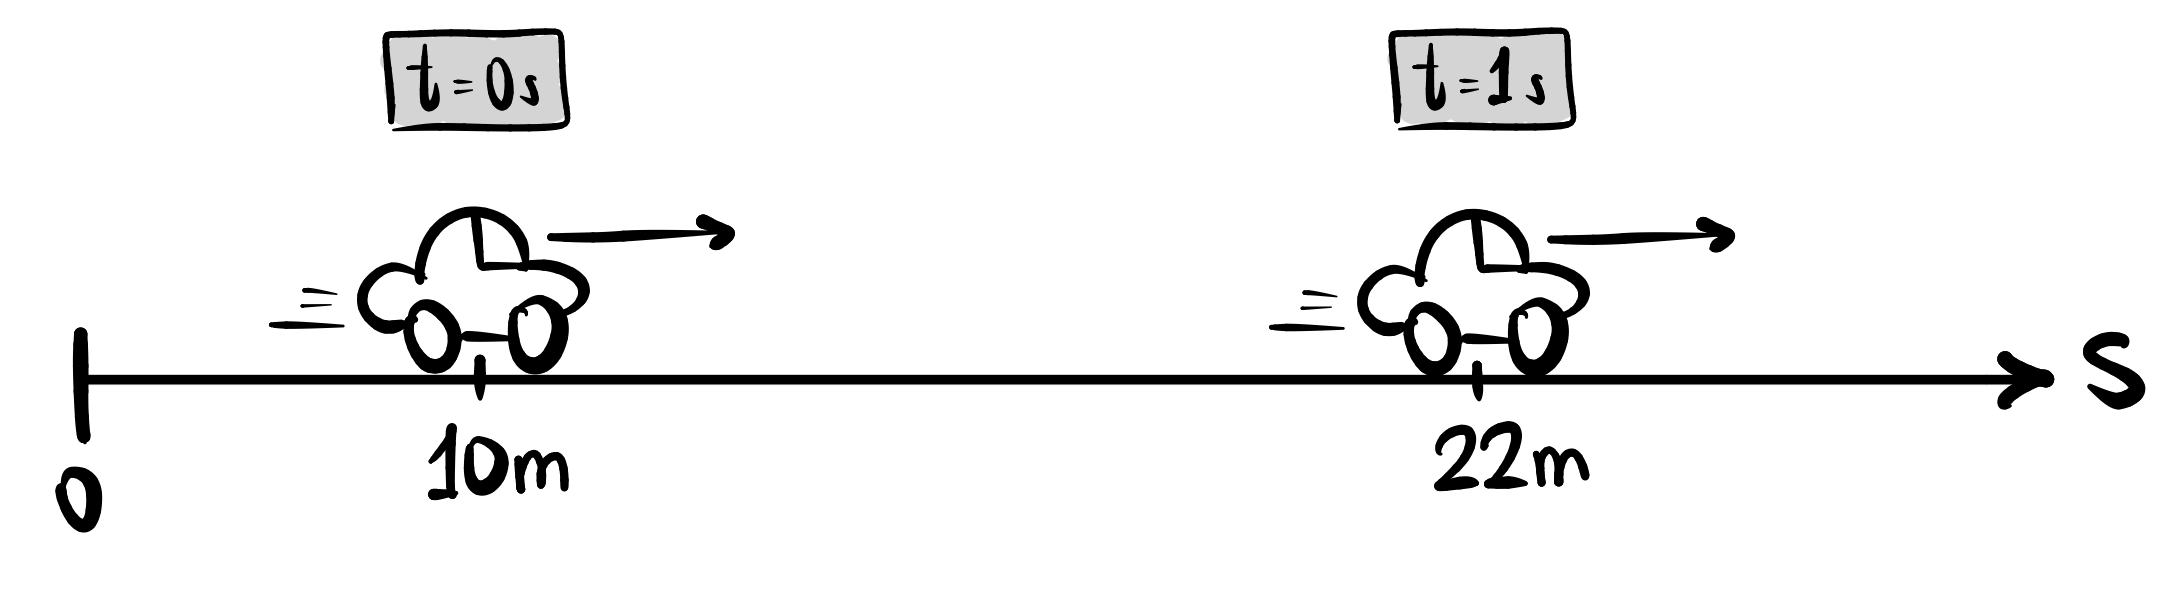
\includegraphics[scale=0.12]{imagensmecanica/mudvsdeltas1.jpeg}
    \caption{Carro em MU em um movimento progressivo.}
    \label{fig_mec_dvsdeltas1}
\end{figure}

A distância é igual ao comprimento da trajetória descrita pelo corpo em movimento. Em um movimento no qual não há inversão no seu sentido, é possível definir a distância como sendo o módulo do deslocamento, ou seja:
$$ d = |\Delta s|.$$

Neste caso, teríamos que $d=|12|=12$m, de modo que a velocidade, usando a Equação \eqref{mecanica_eq_distanciamu}, é dada por:

$$ v=\dfrac{d}{t}=\dfrac{12\text{m}}{1\text{s}}=12 \text{m/s.}$$

Considere agora a situação da Figura \ref{fig_mec_dvsdeltas2}, que é basicamente a mesma, porém de um carro que executa um movimento retrógrado, isto é, ele retrocede no eixo das posições. Calculando seu deslocamento, teríamos $\Delta s = 10-22=-12$m. Munidos disso, podemos calcular sua velocidade usando a Equação \eqref{mecanica_eq_velocidademedia}:

$$ v=\dfrac{\Delta s}{\Delta t}=\dfrac{-12\text{m}}{1\text{s}}=-12 \text{m/s.}$$



\begin{figure}[h]
    \centering
    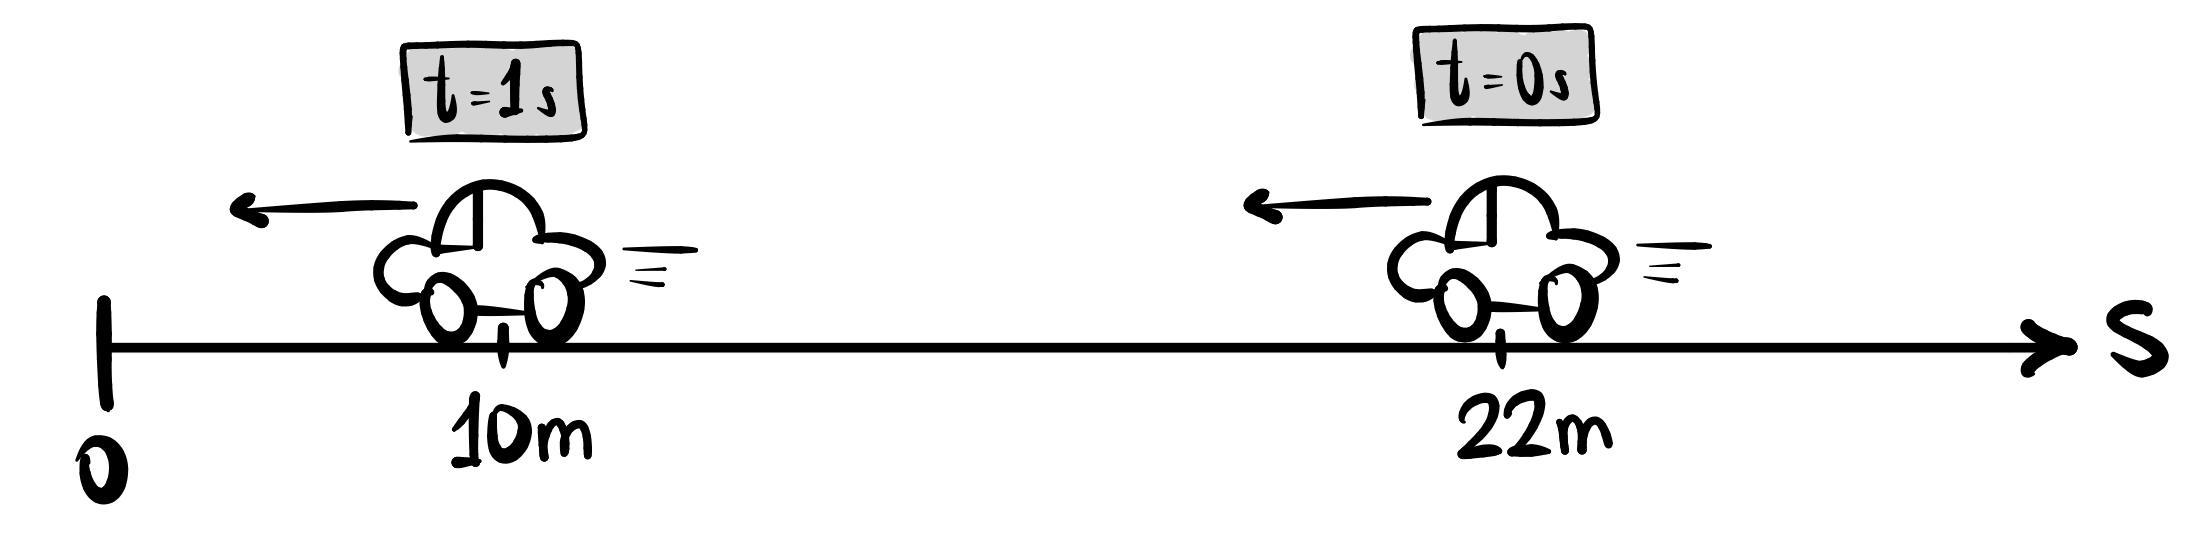
\includegraphics[scale=0.12]{imagensmecanica/mudvsdeltas12.jpeg}
    \caption{Carro em MU em um movimento retrógrado.}
    \label{fig_mec_dvsdeltas2}
\end{figure}


Ou seja, temos um carro que se move com a mesma \textit{rapidez} -- isto é, ele se desloca de 12m a cada 1s -- porém no sentido contrário ao que adotamos como o positivo -- é isso que o sinal negativo da velocidade significa.

Contudo, se fôssemos calcular a distância que o carro percorreu, teríamos que tal valor é $d=|\Delta s| = |-12|=12$m, o que não é de se estranhar: nos dois casos o carro percorreu uma distância de 12 metros. A distância não pode ser um número negativo, haja vista que ela mede um comprimento. Se eu me movo 12 metros para a direita ou para a esquerda a distância que percorri é a mesma nos dois casos: 12 metros.

Dito isso, se fôssemos agora calcular o valor da velocidade do carro usando a Equação \eqref{mecanica_eq_distanciamu}, teríamos:

$$ v = \dfrac{d}{t}=\dfrac{12\text{m}}{1\text{s}}=12 \text{m/s,}$$

\noindent e agora as coisas não concordam mais. O que aconteceu? Calculando a velocidade usando a ideia de deslocamento chegamos em $-12$ m/s, enquanto que usando a ideia de distância, chegamos em $12$ m/s.

Perceba que, na verdade, os resultados não são tão diferentes assim. O valor da velocidade -- a rapidez com que o corpo se move -- é o mesmo nos dois casos, eles só diferem por um sinal. Isso ocorre porque o conceito de velocidade usado nas Equações \eqref{mecanica_eq_velocidademedia} e \eqref{mecanica_eq_distanciamu} não é lá exatamente o mesmo. Veja bem: se a distância nunca pode ser negativa, uma vez que ela é um comprimento -- e foi inclusive definida neste contexto como sendo o módulo do deslocamento, o que é sempre positivo -- a velocidade, se computada por meio de $v=\sfrac{d}{t}$, jamais fornecerá um valor negativo. Nesse sentido, quando olhamos para a equação $d=vt,$ a velocidade que entra ali será sempre positiva -- ela estará medindo, na verdade, a rapidez absoluta com que o corpo se move. Usar a equação $d=vt$ sequer pressupõe que seja adotado um referencial: tanto faz para onde é o sentido positivo convencionado, porque aqui, neste caso, pegaremos sempre o módulo do deslocamento, que é sempre positivo, e isso fará com que a velocidade nunca fique negativa.

Assim, ao usarmos $d=vt$, a velocidade nunca entrará com sinal negativo -- essa é a forma como tal equação foi construída. Logo, para resolver problemas, teremos que avaliar as características geométricas e espaciais deles -- isso porque, como mostram as Figuras \ref{fig_mec_dvsdeltas1} e \ref{fig_mec_dvsdeltas2}, a velocidade, nesse critério, seria de $12$ m/s para os dois casos; ou seja, ela não diferencia quem se move para um lado ou para o outro -- ela olha só a \textit{rapidez com que o corpo se move.}

Já quando usamos a velocidade por meio de $v=\sfrac{\Delta s}{\Delta t},$ o valor absoluto será sempre o mesmo daquele calculado por meio de $v=\sfrac{d}{t},$ podendo diferir deste apenas de um sinal\footnote{Isso vale apenas para o Movimento Uniforme, que é o contexto no qual estamos.}, uma vez que o deslocamento pode ser positivo ou negativo. Assim, a velocidade, quando computada por meio da Equação \eqref{mecanica_eq_velocidademedia}, pressuporá, sempre, a adoção de uma convenção acerca de qual é o sentido positivo, e a velocidade poderá ser positiva ou negativa, a depender se ela aponta no mesmo sentido ou em sentido contrário ao que escolhemos como sendo o positivo.

Nesse sentido, podemos entender a velocidade média definida como sendo a razão entre deslocamento e tempo como um conceito mais completo do que aquele em que a velocidade pudesse ser computada como sendo a distância pelo tempo. Ele é mais completo no sentido que consegue capturar -- através do sinal -- corpos que se movem com a mesma rapidez porém em sentidos diferentes. Quando falamos de distância é impossível capturarmos tal informação, haja vista que se mover 12 metros para a direita ou para a esquerda dá na mesma. 

Como dito no início, essa se tratava de uma conversa um pouco abstrata. A resolução do próximo exemplo deixará mais clara a diferença que pontuamos aqui. Sugiro ao leitor que compare a solução do próximo exemplo com aquela que fizemos deste mesmo problema ao discutir a Equação \eqref{mecanica_eq_distanciamu}.

%Exemplo resolvido

\vspace{0.3cm}

\begin{exemplo}[Nível I]\label{exemplo_funcaohorariaposicaomu01}


Um carro se move com velocidade constante de 20 m/s ao longo de uma rodovia, enquanto outro se move com velocidade constante de 30 m/s, em sentido oposto, ao longo da mesma rodovia.

Se os carros inicialmente estão separados por uma distância de 1.2 km, após quanto tempo eles irão passar um pelo outro?


\resolucao

Sim, este é o mesmo exercício que fizemos anteriormente. Daremos, agora, uma terceira solução para ele. 

\medskip

Para resolver o problema usando a função horária da posição é preciso, antes de tudo, definir uma origem e uma orientação a fim de que as posições possam ser marcadas. Considere a Figura \ref{fig_mec_sorveteexemplo011}, que mostra uma escolha feita: consideramos a origem como sendo a posição inicial do carro $A$ e, consequentemente, a posição inicial de $B$ será $s_0=1200$m, uma vez que os carros estão inicialmente separados por tal distância e o eixo está orientado para direita.

{
\centering
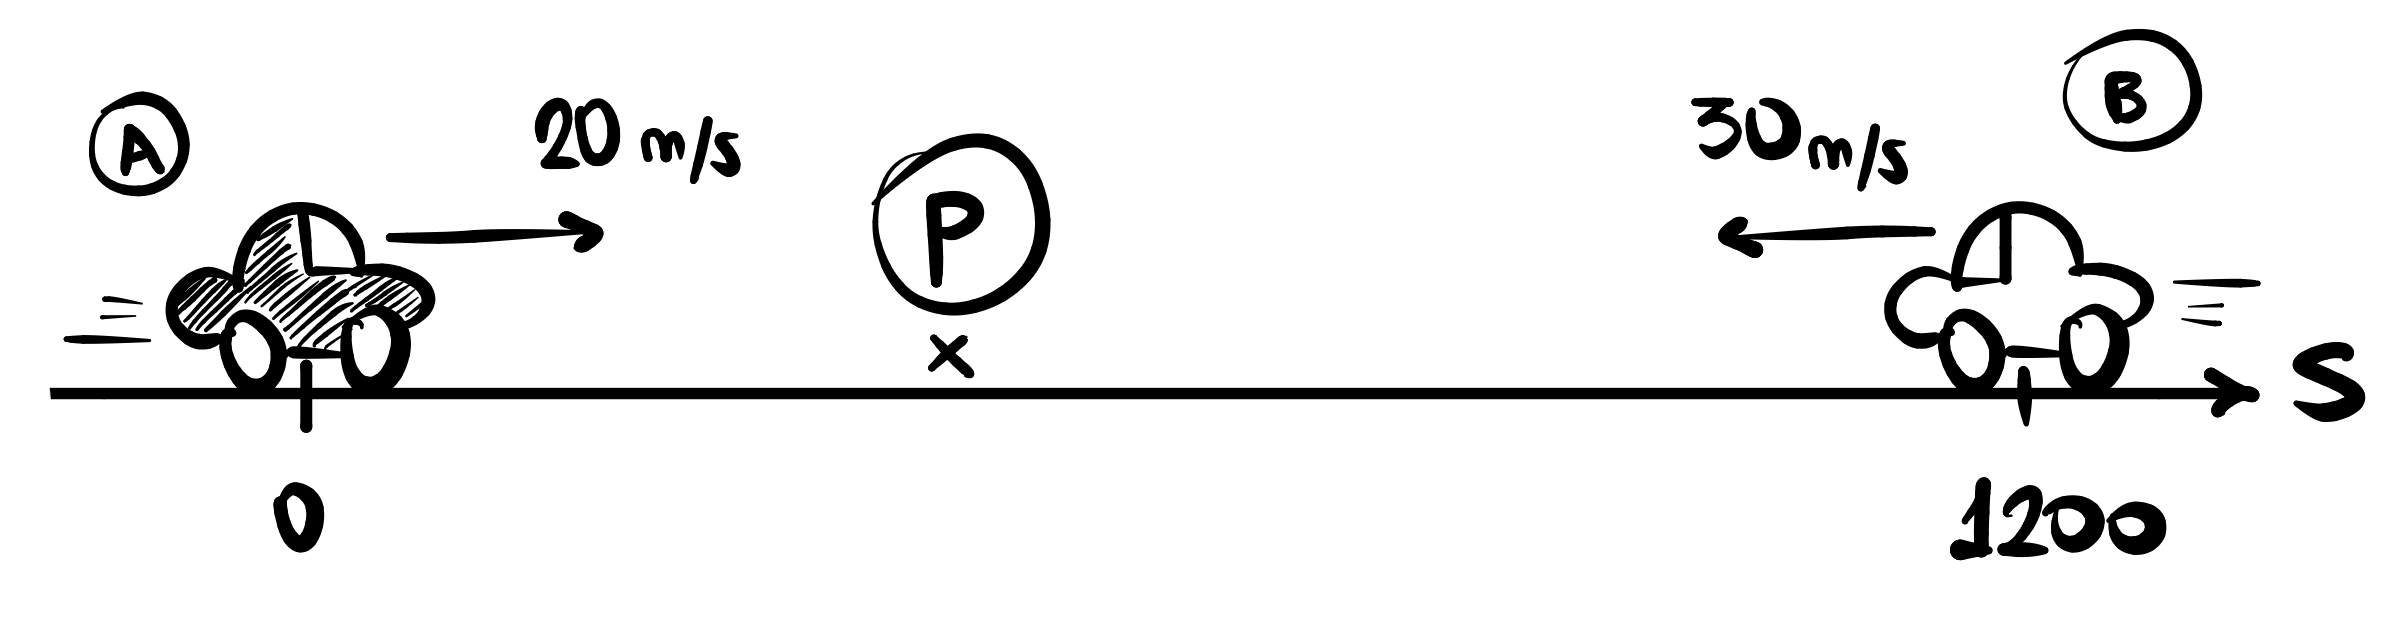
\includegraphics[width=0.6\linewidth]{imagensmecanica/sorveteexemplo011.jpeg}
\captionof{figure}{Referencial orientado para direita com origem na posição inicial do carro A.}
\label{fig_mec_sorveteexemplo011}
} 
\vspace{0.3cm}

Em tal referencial as funções de posição dos carros são:

\begin{enumerate}
    \item [(A)] $s_A= s_0+vt = \cancelto{0}{s_0}+20t \implies \boxed{s_A=20t.}$

    \item [(B)] $s_B= s_0+vt = 1200-30t \implies \boxed{s_B=1200-30t.}$
\end{enumerate}

Ora, dizer que os carros vão passar um pelo outro significa que, em um certo instante $t$, as suas posições irão coincidir -- na posição representada pelo ponto $P$ na figura. Ou seja, os carros se encontram quando $s_A=s_B:$

$$ 20t = 1200-30t \implies 50t = 1200 \implies \boxed{t = 24 \text{ segundos.}}$$

Naturalmente, obtivemos a resposta que já esperávamos. Note que tal resposta independe, é claro, do referencial adotado: o tempo, na mecânica clássica, é absoluto. Assim, se leva 24 segundos para que algo aconteça em um referencial, levará 24 segundos para que isso aconteça em qualquer outra referencial.  


\medskip

Considere, por exemplo, a origem e orientação adotadas no referencial da Figura \ref{fig_mec_sorveteexemplo012}: neste caso alteramos a origem, que agora está a 100 metros para a esquerda de $A.$ Assim, sendo a distância entre os carros inicialmente de $1200$m, a posição do carro $B$ deve ser $100+1200=1300$m, como mostra a figura.

\vspace{0.3cm}
{
\centering
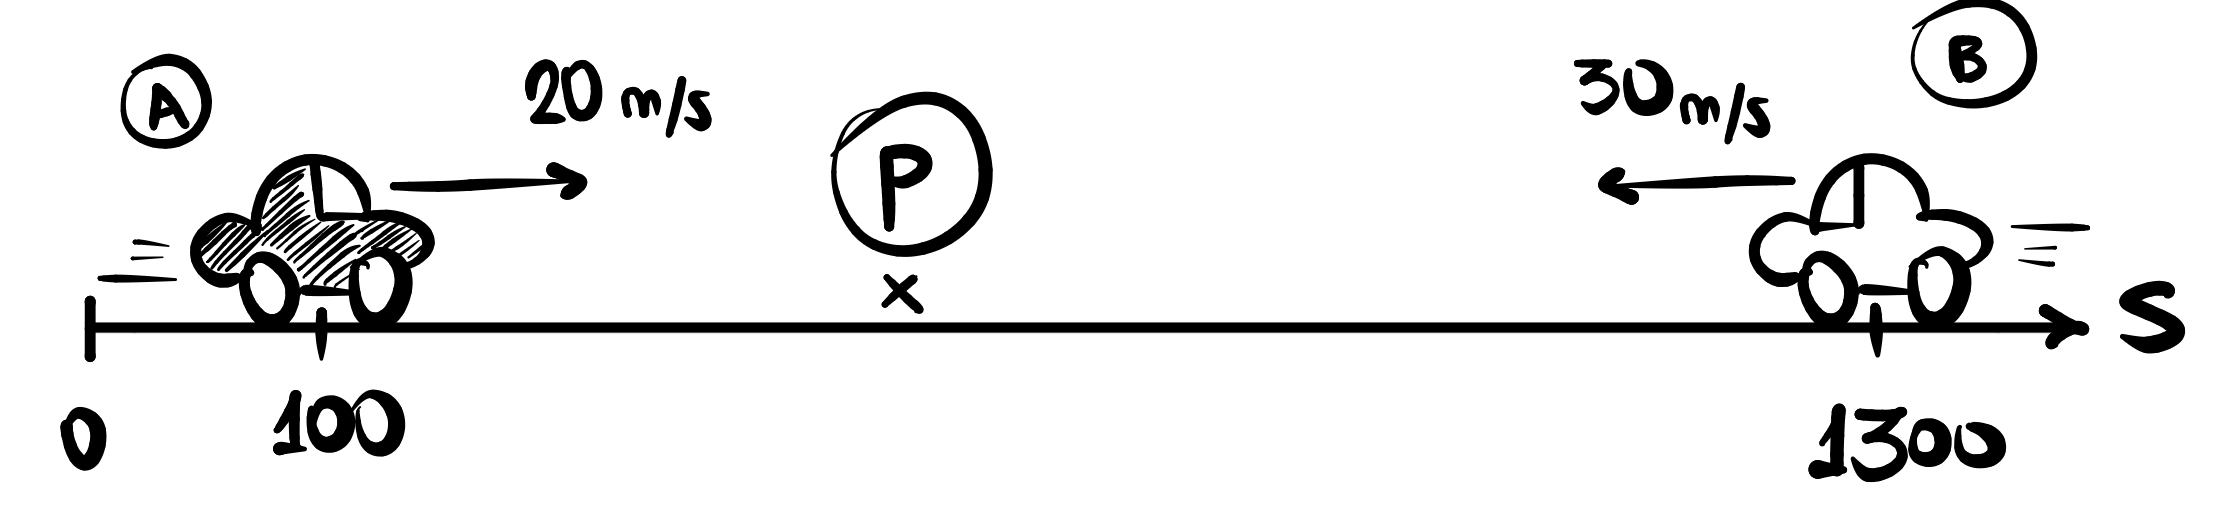
\includegraphics[width=0.6\linewidth]{imagensmecanica/sorveteexemplo012.jpeg}
\captionof{figure}{Referencial orientado para direita com origem arbitrária.}
\label{fig_mec_sorveteexemplo012}
} 
\vspace{0.3cm}

Em tal referencial as funções de posição dos carros são:

\begin{enumerate}
    \item [(A)] $s_A= s_0+vt = 100+20t \implies \boxed{s_A=100+20t.}$

    \item [(B)] $s_B= s_0+vt = 1300-30t \implies \boxed{s_B=1300-30t.}$
\end{enumerate}

Para que eles se encontrem é preciso que $s_A=s_B:$

$$ 100+20t = 1300 - 30t \implies 50t = 1200 \implies \boxed{t = 24 \text{ segundos.}}$$

Logo, adotando uma origem diferente, as funções horárias da posição mudam, mas a nossa resposta final segue sendo a mesma, como deve ser. \\


\medskip

Considere agora um terceiro referencial adotado na Figura \ref{fig_mec_sorveteexemplo013}, que em mudamos não apenas a origem mas também a orientação (note, porém, que as posições iniciais dos carros, por mais arbitrárias que sejam, precisam satisfazer a condição de que suas diferenças sejam de 1200 metros, uma vez que essa é a situação inicial do problema físico.)

\vspace{0.3cm}
{
\centering
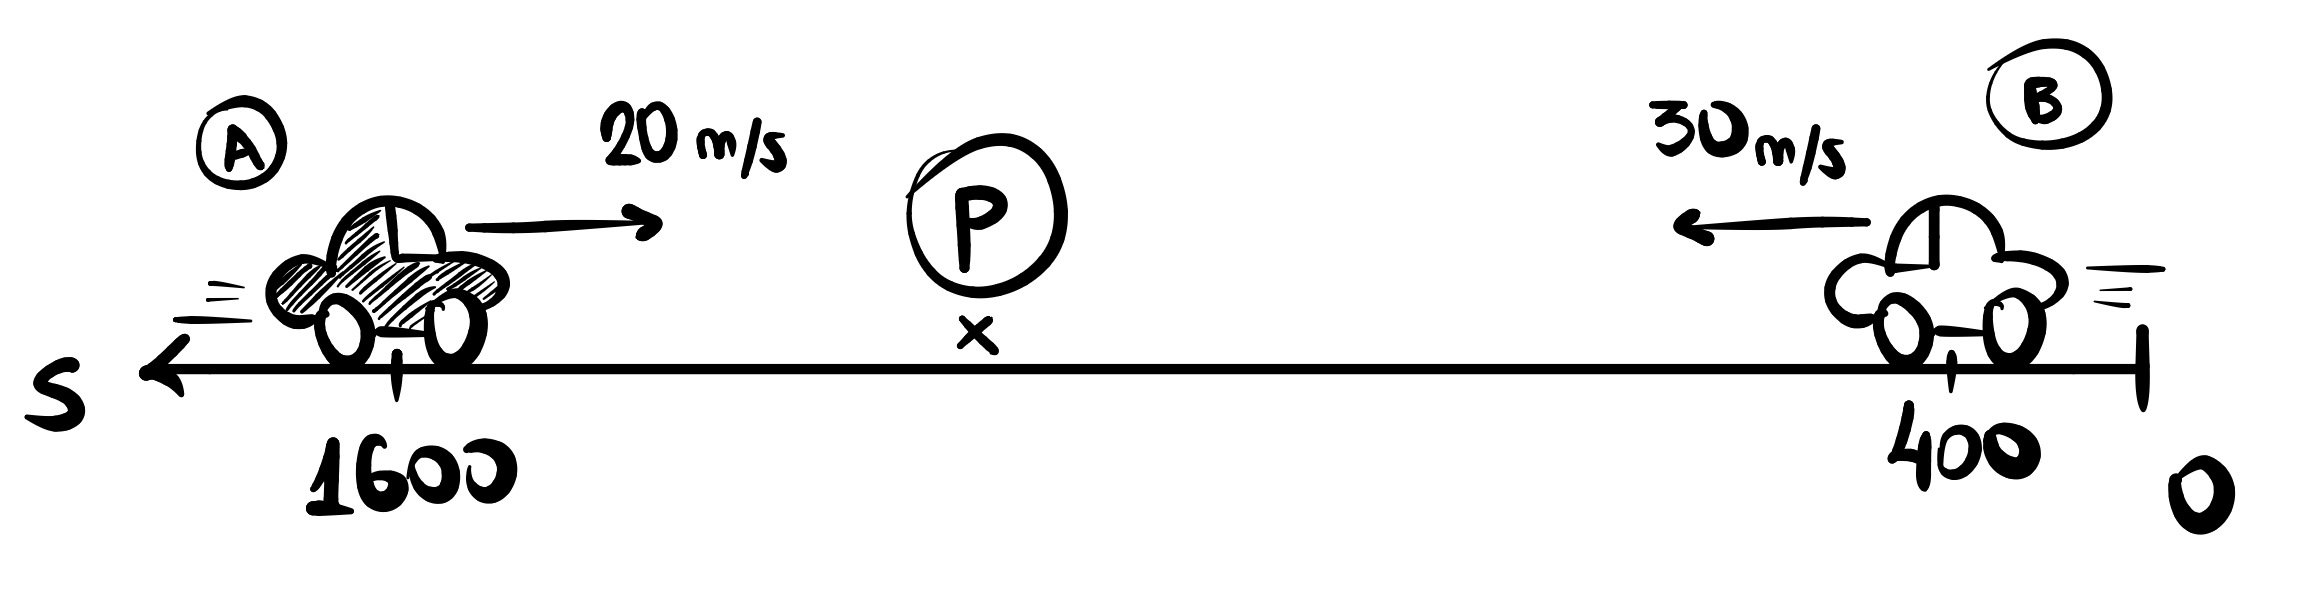
\includegraphics[width=0.6\linewidth]{imagensmecanica/sorveteexemplo013.jpeg}
\captionof{figure}{Referencial orientado para esquerda com origem arbitrária.}
\label{fig_mec_sorveteexemplo013}
} 
\vspace{0.3cm}

Em tal referencial as velocidades para a direita serão negativas, e as velocidades para a esquerda se tornam positivas, de modo que as funções de posição dos carros são:

\begin{enumerate}
    \item [(A)] $s_A= s_0+vt = 1600-20t \implies \boxed{s_A=1600-20t.}$

    \item [(B)] $s_B= s_0+vt = 400+30t \implies \boxed{s_B=400+30t.}$
\end{enumerate}

Para que eles se encontrem é preciso que $s_A=s_B:$

$$ 1600-20t = 400+30t \implies 50t = 1600 - 400 = 1200 \implies \boxed{t = 24 \text{ segundos.}}$$

Ou seja, para computar o intervalo de tempo entre dois eventos é indiferente o referencial adotado -- bastando, para tanto, se atentar aos sinais da velocidade para as diferentes orientações adotadas. Em sistemas de coordenadas (referenciais) distintos as posições iniciais e finais podem ser diferentes, os sinais da velocidade podem mudar, as equações de posição mudam, mas o intervalo de tempo para que algo aconteça é sempre o mesmo.\footnote{A posição no espaço na qual os carros se encontram também é a mesma: a colisão ocorre sempre no mesmo lugar geométrico do espaço. Tal lugar, contudo, receberá atribuições numéricas diferentes a depender da escolha da origem. Como o leitor pode verificar, nos três referenciais escolhidos, as posições de encontro serão, respectivamente, em $s_1=480$m, $s_2=580$m e $s_3=1120$m. O encontro, apesar de ocorrer no mesmo lugar geométrico do espaço, recebe coordenadas diferentes devido às diferentes escolhas de origem e orientação.}
 
 

\end{exemplo}

\vspace{0.3cm}






\begin{exemplo}[Nível II]\label{exemplo_funcaohorariaposicaomu02}


Considere três carros $A, B$ e $C,$ que se movem, respectivamente, com as velocidades $v_A=60$ m/s, $v_B=20$ m/s e $v_C=40$ m/s. O carro $B$ se encontra, inicialmente, $120$ metros a frente do carro $A$; e o carro $C$, por sua vez, $120$ metros a frente do carro $B.$ \\

A partir de tal configuração, após quanto tempo o carro $A$ estará entre $B$ e $C,$ exatamente no meio do caminho entre os dois?


\resolucao

Considere o referencial adotado na Figura \ref{fig_mec_funcaoposicaoexemplo011}, com a origem na posição inicial de $A.$ Em tal referencial as equações de posição são:

\begin{enumerate}
    \item [(A)] $s_A= \cancelto{0}{s_0}+vt \implies s_A=60t.$

    \item [(B)] $s_B= s_0+vt \implies s_B=120+20t.$

    \item [(C)] $s_C= s_0+vt \implies s_C=240+40t.$
\end{enumerate}

{
\centering
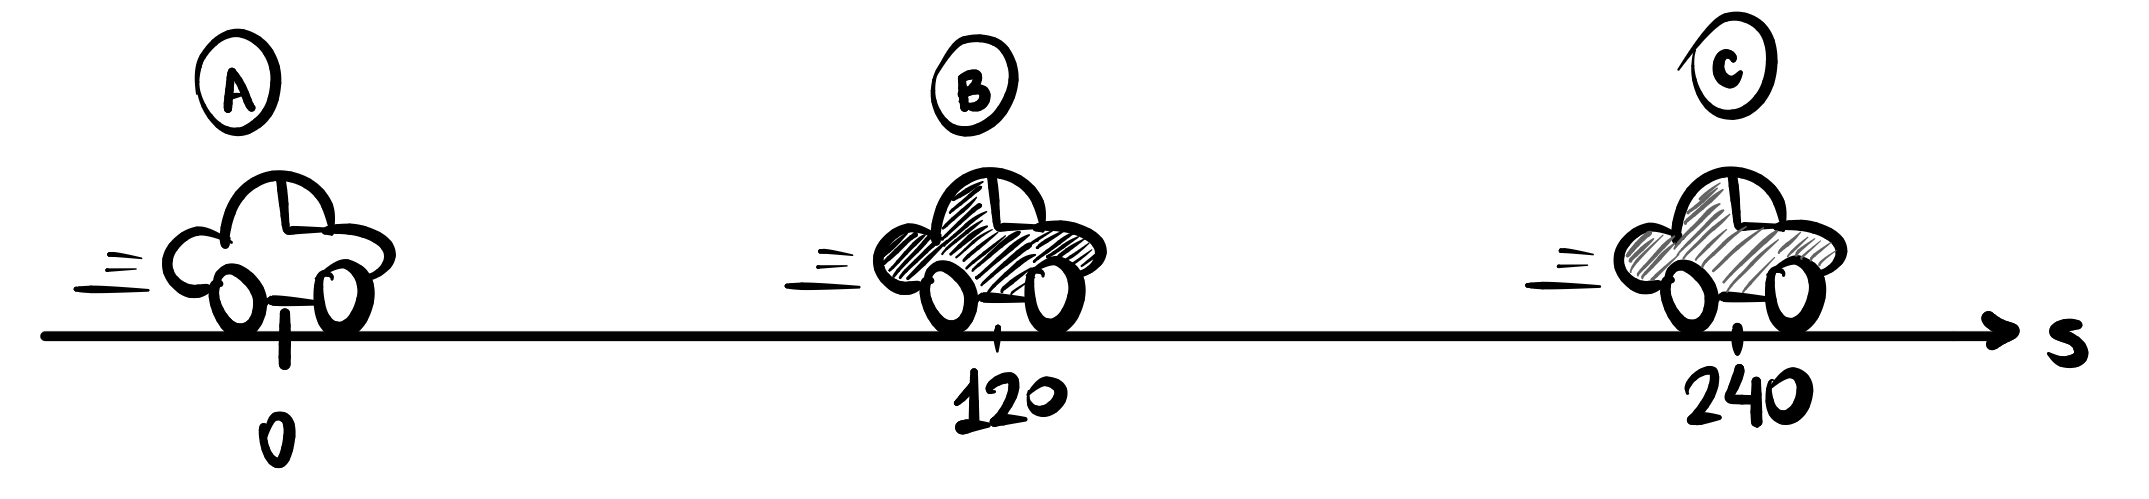
\includegraphics[width=0.6\linewidth]{imagensmecanica/funcaoposicaoexemplo011.jpeg}
\captionof{figure}{Representação do problema com escolha de referencial.}
\label{fig_mec_funcaoposicaoexemplo011}
} 
\vspace{0.3cm}

A configuração buscada é aquela da Figura \ref{fig_mec_funcaoposicaoexemplo012}, na qual, para que $A$ esteja exatamente no meio do caminho entre $B$ e $C$, as distâncias destacadas devem ser iguais, isto é:

$$ s_A-s_B = s_C-s_A,$$
o que nos leva a

$$ s_A = \dfrac{s_B+s_C}{2},$$
ou seja, a posição de $A$ será exatamente a média aritmética das posições de $B$ e $C$ -- ele estará exatamente no meio do caminho.

\vspace{0.3cm}
{
\centering
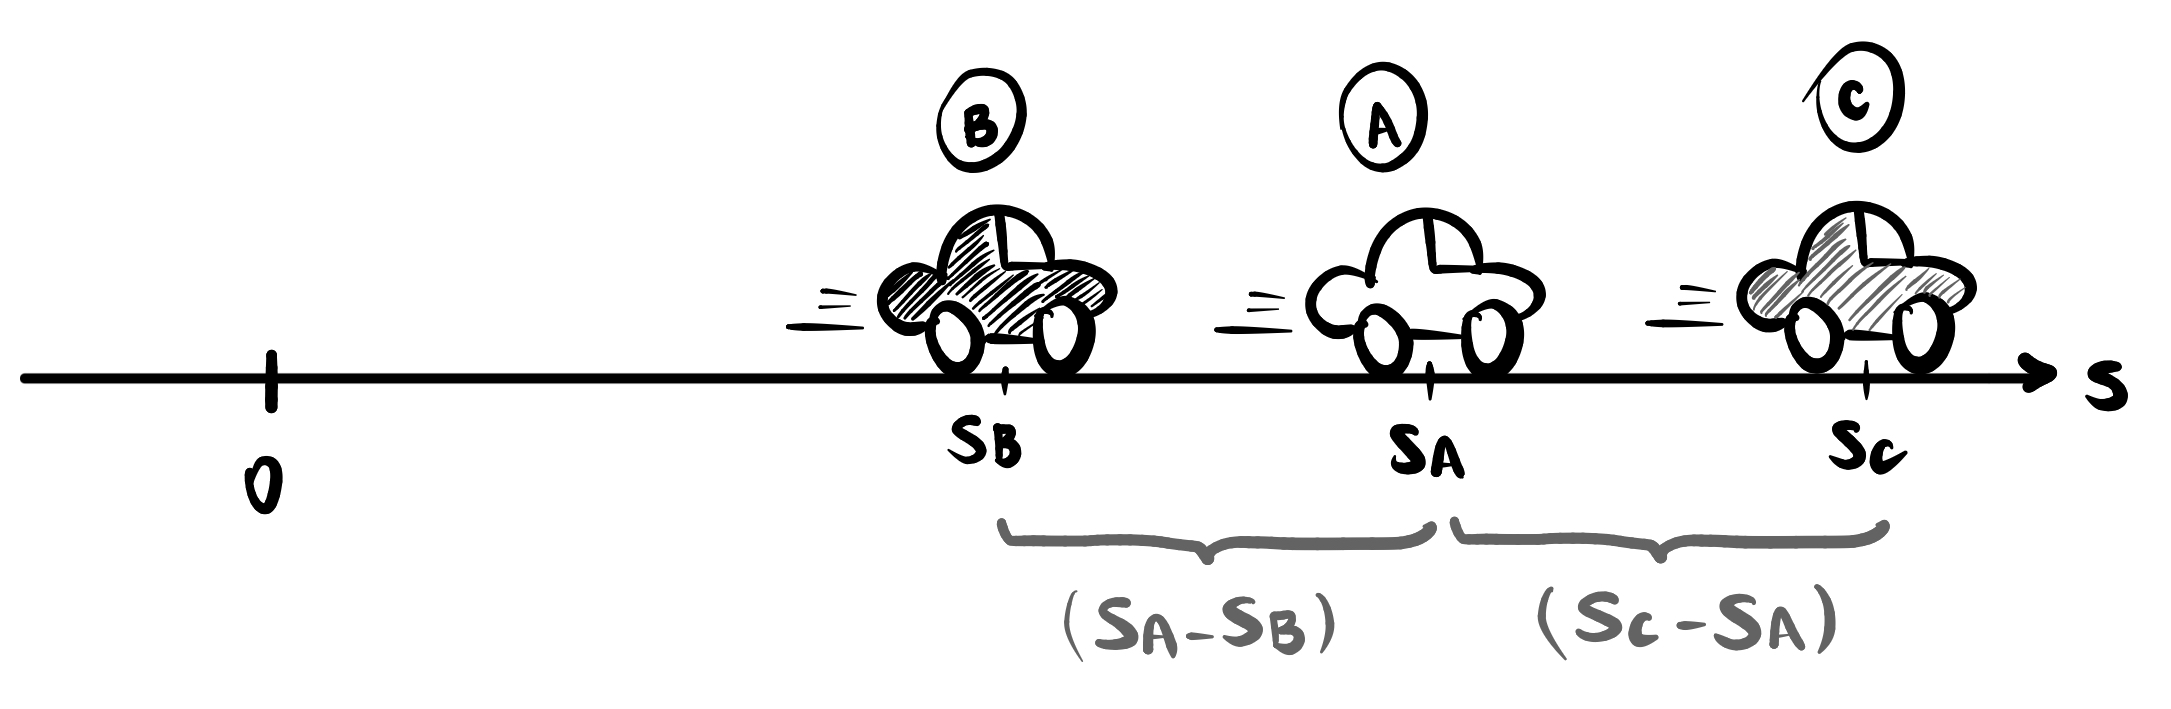
\includegraphics[width=0.6\linewidth]{imagensmecanica/funcaoposicaoexemplo012.jpeg}
\captionof{figure}{Carro $A$ exatamente a meia distância entre os carros $B$ e $C.$}
\label{fig_mec_funcaoposicaoexemplo012}
} 
\vspace{0.3cm}
Usando as equações de posições construídas, chegamos em

$$ s_A = \dfrac{s_B+s_C}{2} \implies 60t = \dfrac{360+60t}{2} \implies \boxed{t = 6 \text{ segundos.}}$$
 
 

\end{exemplo}

\vspace{0.3cm}







\begin{exemplo}[Nível III (ITA - 1985)]\label{exemplo_funcaohorariaposicaomu03}


Um ônibus parte do Rio de Janeiro para Curitiba às $7$ horas da manhã; às $12$ horas parte outro ônibus de Curitiba para o Rio. Percorrem os $720$ km entre as duas cidades em $12$ horas. A hora e a distância do Rio de Janeiro em que os ônibus se encontram, são, respectivamente:
\begin{enumerate}
\item[(a)] $08$h$30$ min e $220$ km.
\item[(b)] $15$h$30$ min e $220$ km.
\item[(c)] $08$h$30$ min e $510$ km.
\item[(d)] $15$h$30$ min e $510$ km.
\item[(e)] $15$h$30$ min e $498$ km.
\end{enumerate}


\resolucao


 Assumindo que os ônibus se movem com velocidade constante, seja $A$ e $B$ os pontos que representam o Rio de Janeiro e Curitiba, respectivamente. Considere um eixo de posições com origem em $A$ e orientado de $A$ para $B$. Logo, nesse sistema, a função horária da posição do ônibus que sai do Rio para Curitiba -- chamemo-lo de ônibus $1$ -- é

$$ s_1 = \cancelto{0}{s_0}+vt \implies s_1(t)=60t,$$

\noindent em que  velocidade de cada ônibus, sendo constante, é dada por

$$ v= \dfrac{d}{\Delta t} = \dfrac{720 \text{ km}}{12 \text{ h}}= 60 \text{ km/h.}$$

A função horária da posição do ônibus que sai de Curitiba para o Rio -- chamemo-lo de ônibus $2$ -- é

$$ s_2 = s_0 + vt' \implies s_2(t)=720-60(t-5).$$

Note que os cronômetros $t$ e $t'$ que cronometram os movimentos completos dos ônibus $1$ e $2$ são diferentes, uma vez que este começa a se mover apenas $5$ horas após o início do movimento daquele. Logo, para ajustar isso, o tempo do segundo ônibus deve ser $t'=t-5$. Perceba que isso está de acordo, porque em $t=5$ h (tempo cronometrado a partir do início do movimento do ônibus $1$) o ônibus $2$ estará iniciando o seu movimento, isto é, estará em $t'=t-5=0.$

Sendo assim, os ônibus se encontram quando $s_1(t)=s_2(t),$ ou seja:

$$ 60t = 720-60(t-5) \implies \boxed{t=8.5 \text{ h},}$$

\noindent e, como o tempo $t$ foi medido a partir do início do movimento do ônibus $1$, isto é, $t=0$ era às 07h00, então o horário do encontro ocorre em $07\text{h}00+08\text{h}30=15\text{h}30.$

A posição do encontro ocorre em

$$ s_1(t) = 60t =  \boxed{510 \text{ km}.}$$

Sendo a origem do sistema de coordenadas no Rio de Janeiro, a distância do ponto de encontro ao Rio é dada exatamente por $510$ km.
 

\end{exemplo}

\vspace{0.3cm}















\newpage




\section{Movimento Uniformemente Variado}

Tal movimento é \textbf{definido}\footnote{Ou seja, estamos criando vocabulário: dando um nome específico a um tipo específico de movimento.} como sendo aquele no qual o \textbf{valor da aceleração do objeto é constante}. Ou seja, como mostra a Figura \ref{fig_mec_muv}, a velocidade irá variar de quantidades iguais em iguais intervalos de tempo. Em tal exemplo, para quaisquer intervalos de tempo que o leitor escolher, o valor da aceleração será sempre o mesmo. Façamos alguns cálculos, a fim de tornar isso claro. Considerando o intervalo de tempo de $0$s a $1$s, teríamos:

$$ a_{1} = \dfrac{\Delta v}{\Delta t} = \dfrac{4-2}{1-0} = \dfrac{2 \text{m/s}}{1\text{s}} = 2 \text{m/s}^2.$$

Considerando agora intervalo de tempo de $1$s a $2$s, teríamos:

$$ a_{2} = \dfrac{\Delta v}{\Delta t} = \dfrac{6-4}{2-1} = \dfrac{2 \text{m/s}}{1\text{s}} = 2 \text{m/s}^2.$$

Se avaliarmos agora no intervalo de tempo total do movimento, de $0$s a $3$s, teríamos:

$$ a_{3} = \dfrac{\Delta v}{\Delta t} = \dfrac{8-2}{3-0} = \dfrac{6 \text{m/s}}{3\text{s}} = 2 \text{m/s}^2,$$

\noindent ou seja, o padrão de variação da velocidade é claro: ela muda sempre a uma mesma taxa, qualquer que seja o intervalo de tempo em que avaliarmos o movimento. Isso é o que define o movimento uniformemente variado.

\begin{figure}[h]
    \centering
    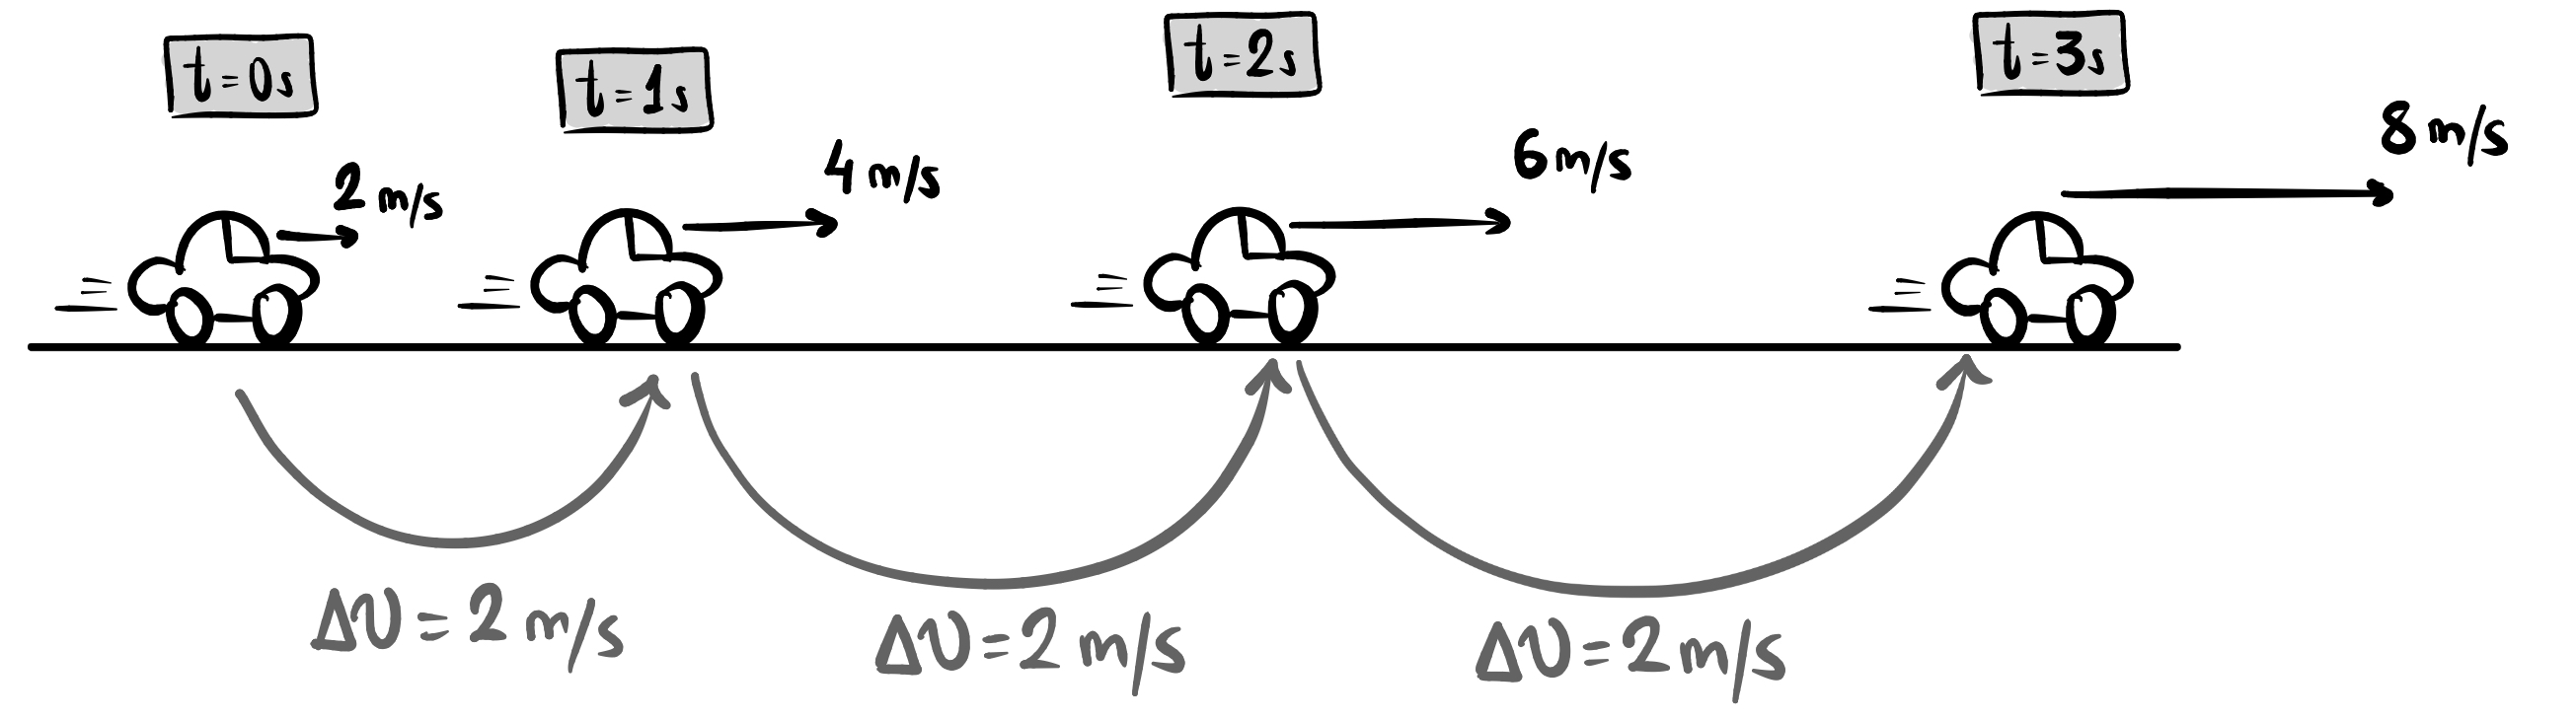
\includegraphics[scale=0.15]{imagensmecanica/muvexemplo.jpeg}
    \caption{O movimento com aceleração constante}
    \label{fig_mec_muv}
\end{figure}

Contudo, é importante que fique claro também o que \textbf{não é} um movimento uniformemente variado, e a Figura \ref{fig_mec_muvcontraexemplo} ilustra um exemplo. Perceba que trata-se um movimento acelerado -- isto é, no qual a velocidade varia -- porém a forma como a velocidade varia não é a mesma o tempo inteiro. Note que, se fôssemos calcular o valor da aceleração do corpo, não teríamos um único valor. 


\begin{figure}[h]
    \centering
    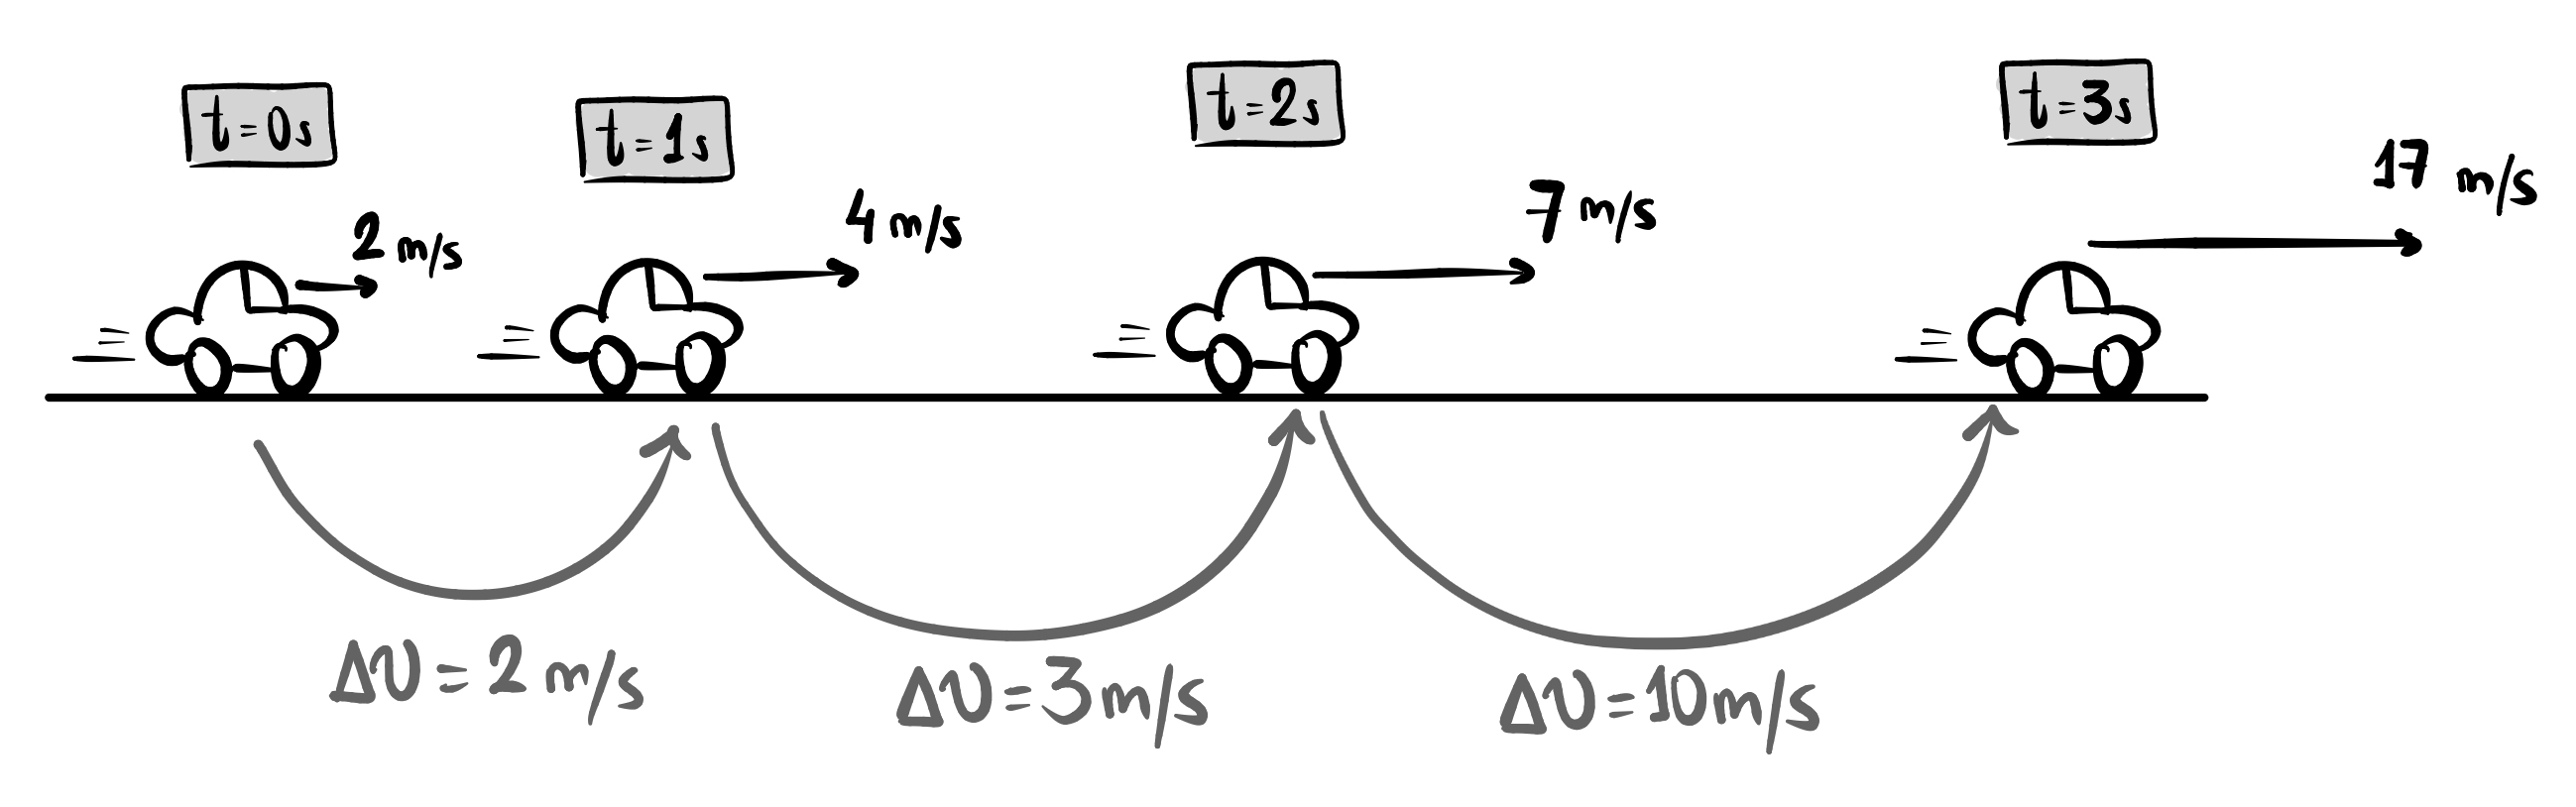
\includegraphics[scale=0.15]{imagensmecanica/muvcontraexemplo.jpeg}
    \caption{O movimento acelerado que não é uniformemente variado.}
    \label{fig_mec_muvcontraexemplo}
\end{figure}


Considerando o intervalo de tempo de $0$s a $1$s, teríamos:

$$ a_{1} = \dfrac{\Delta v}{\Delta t} = \dfrac{4-2}{1-0} = \dfrac{2 \text{m/s}}{1\text{s}} = 2 \text{m/s}^2.$$

Agora, avaliando no intervalo de tempo de $1$s a $2$s, teríamos:

$$ a_{2} = \dfrac{\Delta v}{\Delta t} = \dfrac{7-4}{2-1} = \dfrac{3 \text{m/s}}{1\text{s}} = 3 \text{m/s}^2.$$

E, se avaliássemos no intervalo de tempo total,  de $0$s a $3$s, teríamos:

$$ a_{3} = \dfrac{\Delta v}{\Delta t} = \dfrac{17-2}{3-0} = \dfrac{15 \text{m/s}}{3\text{s}} = 5 \text{m/s}^2.$$


Note que, neste caso, a velocidade varia, porém não de uma forma constante -- o incremento da velocidade para um mesmo intervalo de tempo é cada hora um, de modo que tal movimento é acelerado, porém não é uniformemente variado.

Agora que está claro do que se trata um movimento uniformemente variado, podemos analisar as equações que o descrevem.








\begin{secnivel}[Função Horária da Velocidade no MUV]
{I}{Função Horária da Velocidade do Movimento Uniformemente Variado}
 

  \eqLdois{dem}{mecanica_eq_muvfuncaovelocidade}{v=v_0+at}
  
\end{secnivel}







\secgfe{De onde vem}

Observe a Figura \ref{fig_mec_funcaovelocidade02}, na qual temos um objeto que se move em um Movimento Uniformemente Variado (MUV) com velocidade inicial $v_0$ no instante inicial $t_0=0$s, alcançando uma velocidade $v$ no instante $t$. Queremos uma equação em que, sabendo o valor da aceleração $a$ do objeto e sua velocidade inicial $v_0$, possamos encontrar, para qualquer instante de tempo futuro $t$, o valor da sua velocidade $v$ naquele instante.

\begin{figure}[h]
    \centering
    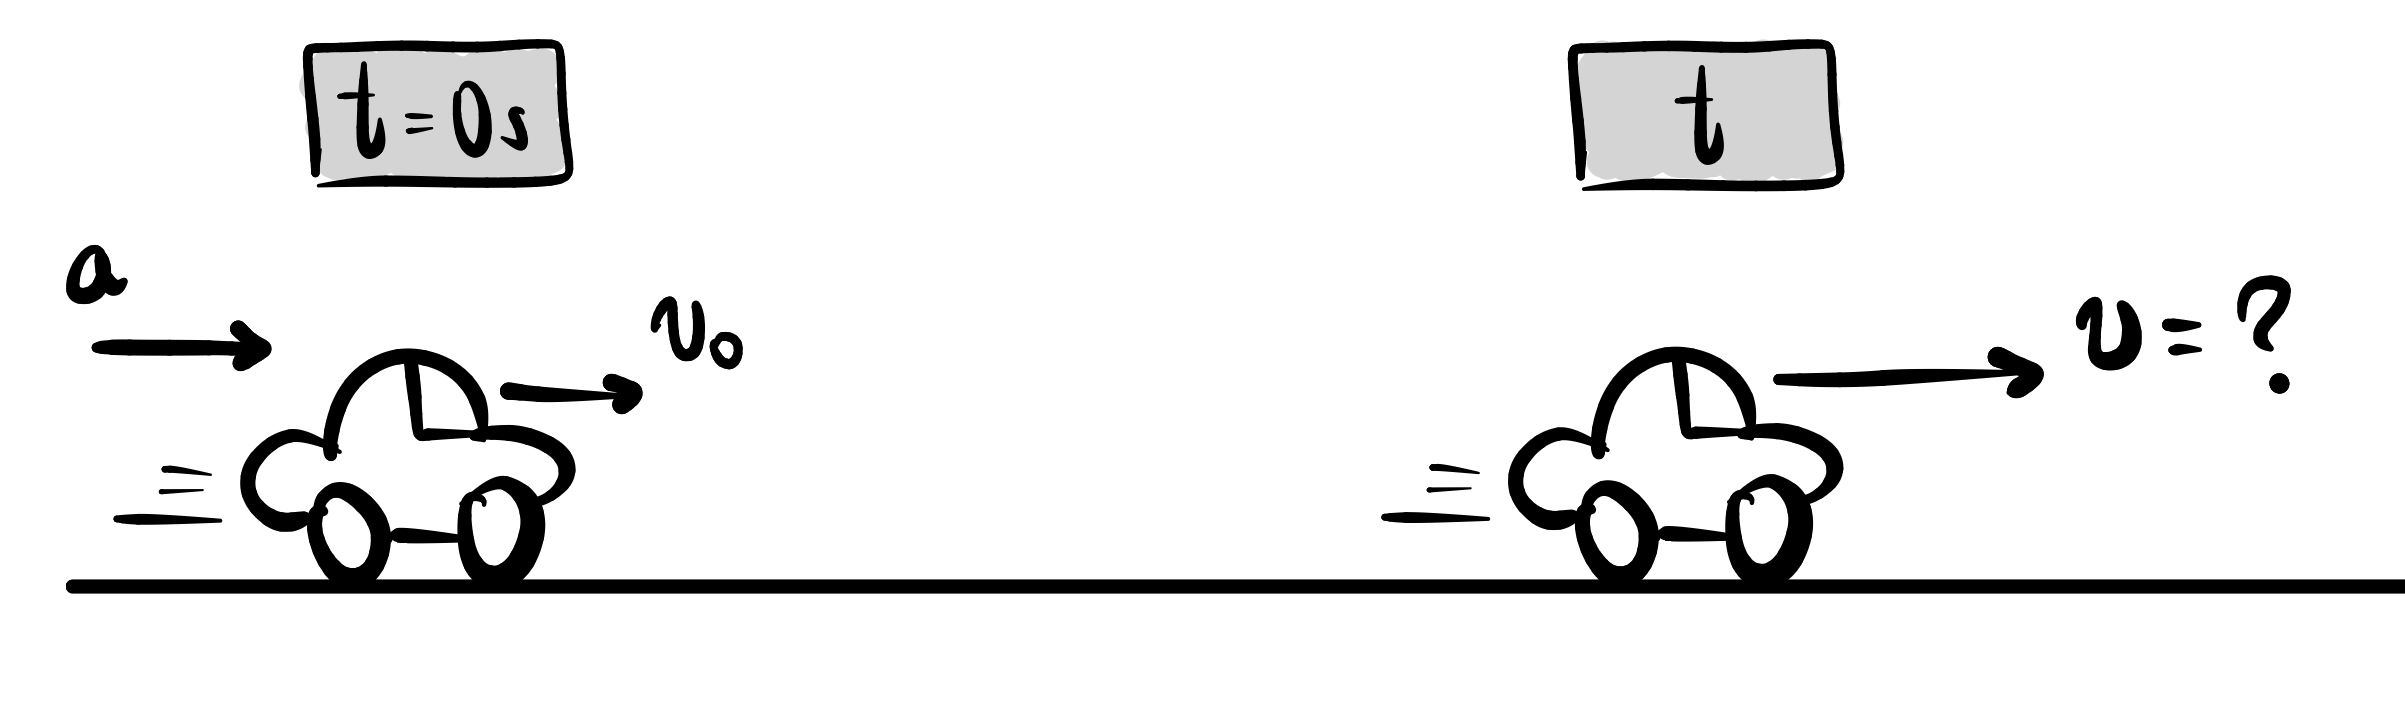
\includegraphics[scale=0.12]{imagensmecanica/muvfuncaovelocidade02.jpeg}
        \caption{A construção da função horária da velocidade para o MUV.}
    \label{fig_mec_funcaovelocidade02}
\end{figure}

A equação que vamos construir é uma consequência natural da definição de aceleração e da forma como definimos o MUV. Note que, pela Equação \eqref{mecanica_eq_aceleracaomedia}, temos que

$$ a_M = \dfrac{\Delta v}{\Delta t} =\dfrac{v-v_0}{t-0}, $$

\noindent contudo, sendo o movimento um MUV, a aceleração $a$ é constante o tempo inteiro, de modo que a aceleração média em qualquer intervalo de tempo será sempre igual a $a$, uma vez que a aceleração nunca muda. Assim, teremos

$$ a_M = a = \dfrac{v-v_0}{t-0} \implies \boxed{v = v_0 + at.} $$

Mais uma vez, vale destacar a finalidade de tal equação: de modo geral, conhecemos quem é a velocidade inicial $v_0$ de um certo objeto, qual é o valor de sua aceleração $a$ e, com tal equação, podemos descobrir o valor de sua velocidade $v$ para qualquer instante futuro de tempo $t$. Desse modo, tal equação é uma função do tempo, e poderíamos escrevê-la de modo a deixar isso explícito como

$$ v(t) = v_0+at,$$
ou seja, $v_0$ e $a$ são os coeficientes de tal função afim, $t$ é a sua variável e, para cada valor de $t$ a equação de retorna um valor de $v$ associado a ele: o valor da velocidade do móvel naquele instante específico. De modo mais concreto, considere um movimento acelerado em que a aceleração é $a=3$ m/s$^2$ e a velocidade inicial é $v_0=5$ m/s. Logo, a função horária da velocidade de tal movimento é

$$ v(t) = 5+3t.$$

Ou seja, com tal equação é possível saber o valor da velocidade $v$ do carro em $t=3$s, que seria de $14$ m/s; ou em  $t=25$s, que seria de $80$ m/s. De modo geral, tal equação fornece a velocidade do móvel para qualquer instante de tempo que se queira.



\secgfe{Onde é usada}

Usamos essa equação em diversos problemas de MUV nos quais estamos interessados em computar a velocidade do objeto que executa tal movimento. Considere, por exemplo, o contexto da Figura \ref{fig_mec_funcaovelocidade01}, no qual um carro executa um MUV. Como poderíamos proceder caso quiséssemos saber a sua velocidade no oitavo segundo do movimento?

\begin{figure}[h]
    \centering
    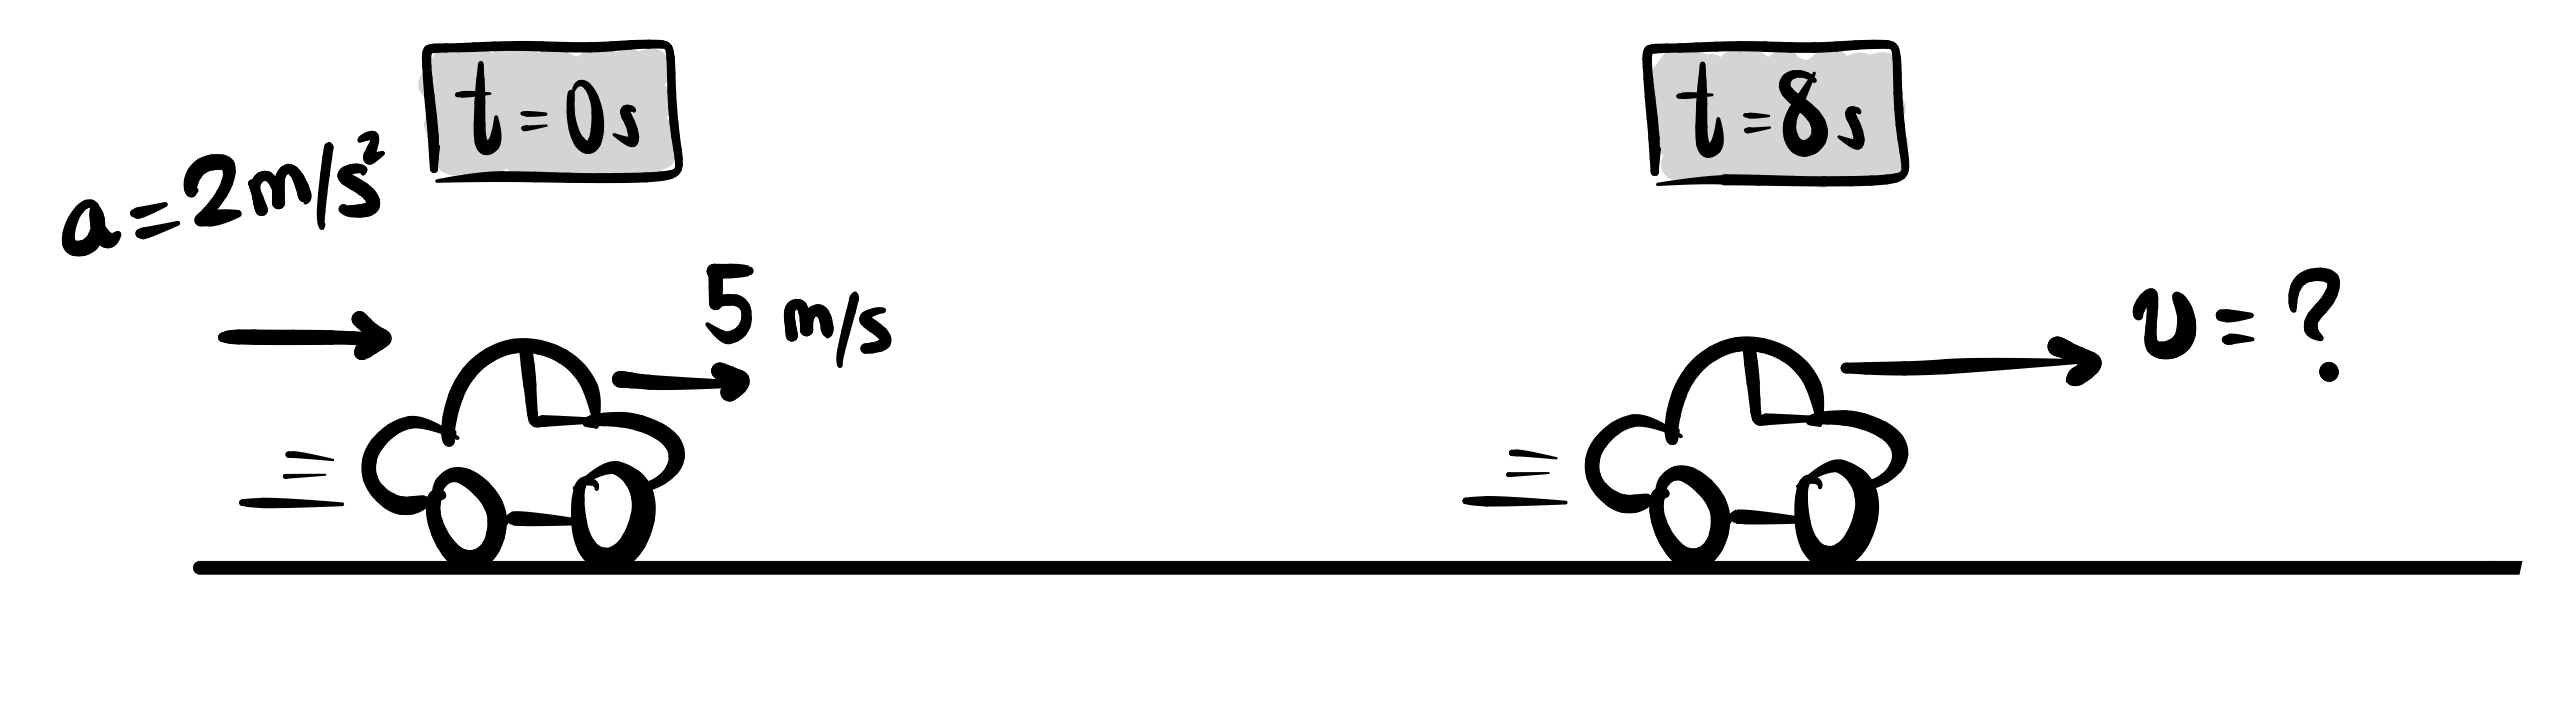
\includegraphics[scale=0.12]{imagensmecanica/muvfuncaovelocidade01.jpeg}
    \caption{Exemplo de um MUV.}
    \label{fig_mec_funcaovelocidade01}
\end{figure}

Ora, isso é justamente o que faz a função horária da velocidade:

$$v(t)=v_0+at \implies v(t) = 5 + 2t.$$

Munidos de tal equação, podemos descobrir o valor da velocidade do carro em qualquer instante. Em particular, para $t=8$s, teríamos

$$ v(8)=5+2\cdot 8= 21 \text{m/s}.$$


\secgfe{Erros comuns}

Os erros mais comuns no uso de tal equação consistem em:

\begin{itemize}
    \item [(i)] Confusão com o instante inicial.

    Note que, na própria demonstração da Equação \eqref{mecanica_eq_muvfuncaovelocidade}, definimos que em $t_0=0$s o valor da velocidade era $v_0.$ Logo, para usarmos corretamente tal equação neste formato, é preciso levar isso com rigor. Note, por exemplo, o MUV representado na Figura \ref{fig_mec_muvfuncaovelocidade04}. Está nítido que se trata de um MUV, no qual a aceleração vale $a=2$m/s$^2,$ como o leitor bem pode verificar. 
    
\begin{figure}[h]
    \centering
    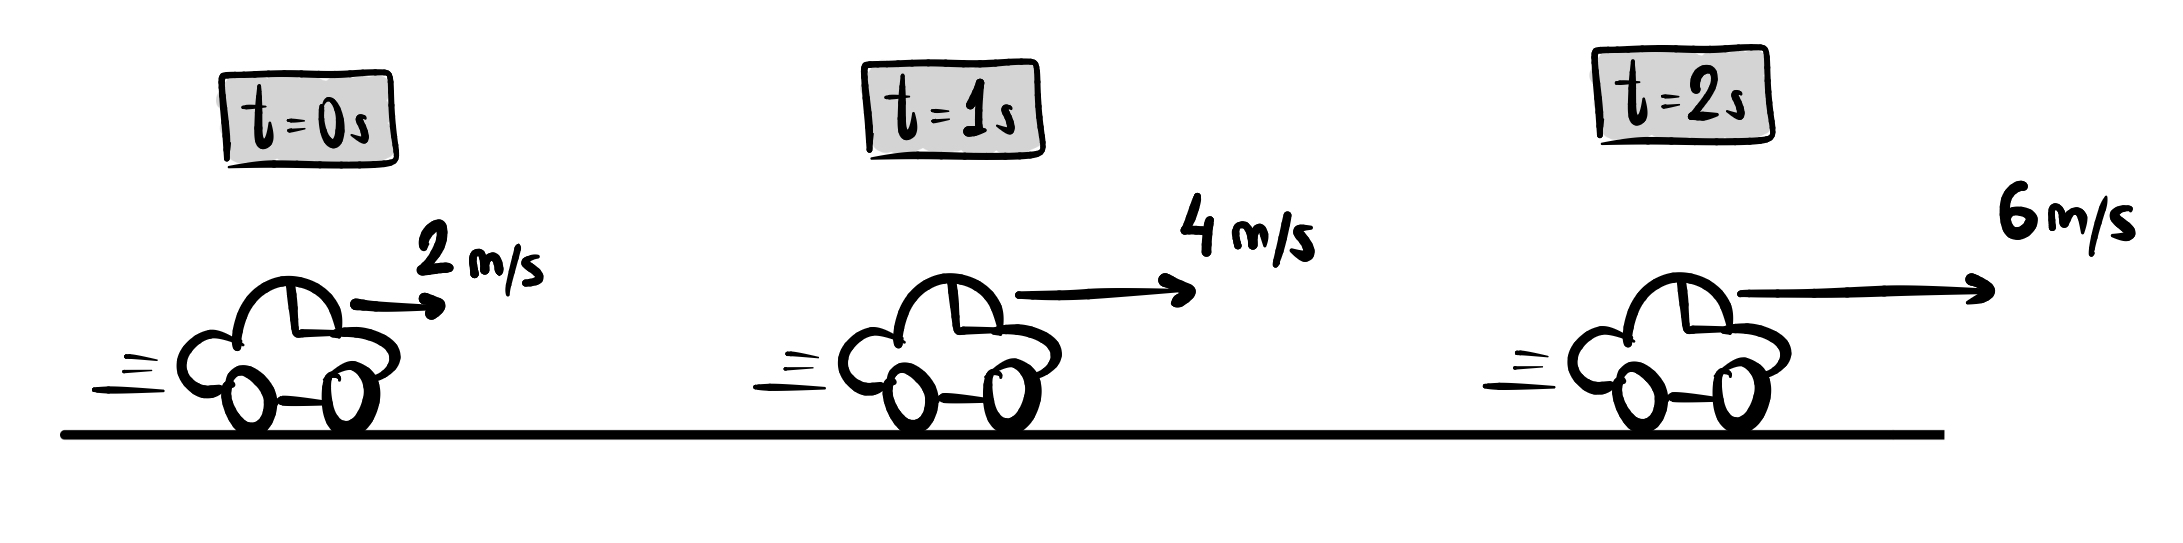
\includegraphics[scale=0.12]{imagensmecanica/muvfuncaovelocidade04.jpeg}
    \caption{Vários instantes para equacionar a função horária da velocidade do MUV.}
    \label{fig_mec_muvfuncaovelocidade04}
\end{figure}

     Contudo, ao escrever a função horária da posição, algum leitor poderia querer ignorar o instante inicial $t=0$s, e escrevê-la a partir do instante $t=1$s, considerando, portanto, o valor de $v_0$ como sendo igual a $4$ m/s, chegando na equação:

     $$ v(t) = 4 +2t.$$

     É imediato perceber que tal equação está errada e não condiz com o contexto, uma vez que, fazendo $t=0$s, chegaríamos em $v(0)=4$m/s, o que claramente está errado, pois $v(0)=2$m/s, como mostra a figura. O erro aqui, portanto, foi não considerar o valor de velocidade inicial como sendo aquele em $t_0=0$s. A equação em que o instante inicial é $t=1$s -- ou qualquer outro -- até pode ser construída, mas não será aquela mesma da Equação \eqref{mecanica_eq_muvfuncaovelocidade}. Neste caso, teríamos que fazer um ajuste e trocar $t$ por $t'=t-1.$ Isso faz a correção para que o novo instante inicial ($t=1$s) seja exatamente $t'=1-1=0$s, ou seja, o instante zero.\footnote{Isso é importante porque o instante de tempo multiplica a aceleração -- o produto $at$ -- e isso representa o incremento de velocidade. Logo, deve-se ter sempre $t=0$ no instante inicial para zerar a variação da velocidade. Uma vez que estamos no instante inicial da análise, não houve, ainda, variação da velocidade.} Neste caso, a equação correta seria:

     $$ v(t') = v_0 + at' \implies v(t)= 4 + 2(t-1).$$
     
     Neste caso, é fácil ver que $v(1) = 4$ m/s, o que concorda com o esperado: em $t=1$s a velocidade é de 4 m/s. 
     
     
     Para o leitor que achou tudo isso complicado demais, fica, portanto, o aviso: para não incorrer neste tipo de complicação e usar sempre a Equação \eqref{mecanica_eq_muvfuncaovelocidade} exatamente naquele formato como construímos, o valor da velocidade inicial $v_0$ deve ser aquele em $t_0=0$s.
     
    \item [(ii)]
     Usar tal equação em contextos nos quais ela não se aplica.

     Faremos aqui uma digressão um pouco mais abstrata, de modo que esse trecho pode ser pulado em uma primeira leitura. Lembre-se que estamos dentro do tópico de Movimento Uniformemente Variado. Correndo o risco de me tornar repetitivo, tal equação é a Função Horária da Velocidade do Movimento Uniformemente Variado -- ou seja, ela serve para computar a velocidade apenas de um corpo que executa um tipo específico de movimento: o movimento com aceleração constante.

     Tentar aplicá-la para outros tipos de movimento levará, naturalmente, a resultados errados. A bem da verdade, se aplicarmos ela para o Movimento Uniforme, até chegamos em um resultado correto. Lembre-se que tal movimento é definido como sendo aquele no qual a velocidade não varia, ou seja, sua aceleração é zero:

     $$ v(t) = v_0 + \cancelto{0}{a} \cdot t \implies \boxed{v(t)=v_0.}$$

     O resultado diz que a velocidade $v(t)$ para qualquer instante de tempo $t$ é igual à velocidade inicial $v_0$, ou seja, tal valor de velocidade é constante e nunca muda -- este é o Movimento Uniforme, e é claro que isso nós já sabíamos. Note, contudo, que, apesar de usarmos a equação ``errada'', nós só chegamos a uma conclusão certa porque, na verdade, o MU é um caso particular do MUV: o Movimento Uniforme é um Movimento Uniformemente Variado em que a aceleração é zero. Logo, todas as equações do MUV, se colocarmos a aceleração igual a zero, devem recair nas equações do MU.\footnote{O leitor pode ver isso como uma grande vantagem: é preciso conhecer só um par de equações -- as funções da posição e da velocidade do MUV, haja vista que as mesmas funções para o MU estão contidas naquelas, bastando, para obtê-las, fazer a aceleração igual a zero. Faça o mesmo exercício, na próxima seção, e obtenha a função da posição do MU a partir daquela do MUV.}

     Tirando este caso particular, em qualquer outro contexto no qual o leitor tentar aplicar a função horária da velocidade do MUV, ele incorrerá em graves erros.
    
    
\end{itemize}


\secgfe{Observações}

Cabe pontuar algumas observações a respeito dos sinais de algumas grandezas na equação. Como já sabemos, o sinal de uma grandeza cinemática -- velocidade ou aceleração -- irá depender do referencial adotado (origem e orientação). Desse modo, é possível escrever a função horária da posição para um certo movimento de mais de uma forma. Observe, para tanto, a Figura \ref{fig_mec_muvfuncaovelocidadesinal01}. Perceba que, nas duas imagens, trata-se exatamente do mesmo movimento -- o que muda é apenas o sistema de orientação: o referencial. Assim, para o referencial da imagem da cima, a velocidade inicial seria positiva, porém a aceleração negativa, de modo que a equação horária da velocidade seria

$$ v(t)=5-2t.$$

A velocidade em um certo instante, digamos $t=5$, seria, portanto, $v(5)=-5$ m/s. Perceba que o sinal negativo, uma vez que o sentido adotado como positivo foi para direita, está indicando apenas que tal velocidade aponta para a esquerda, com intensidade de 5 m/s.



\begin{figure}[h]
    \centering
    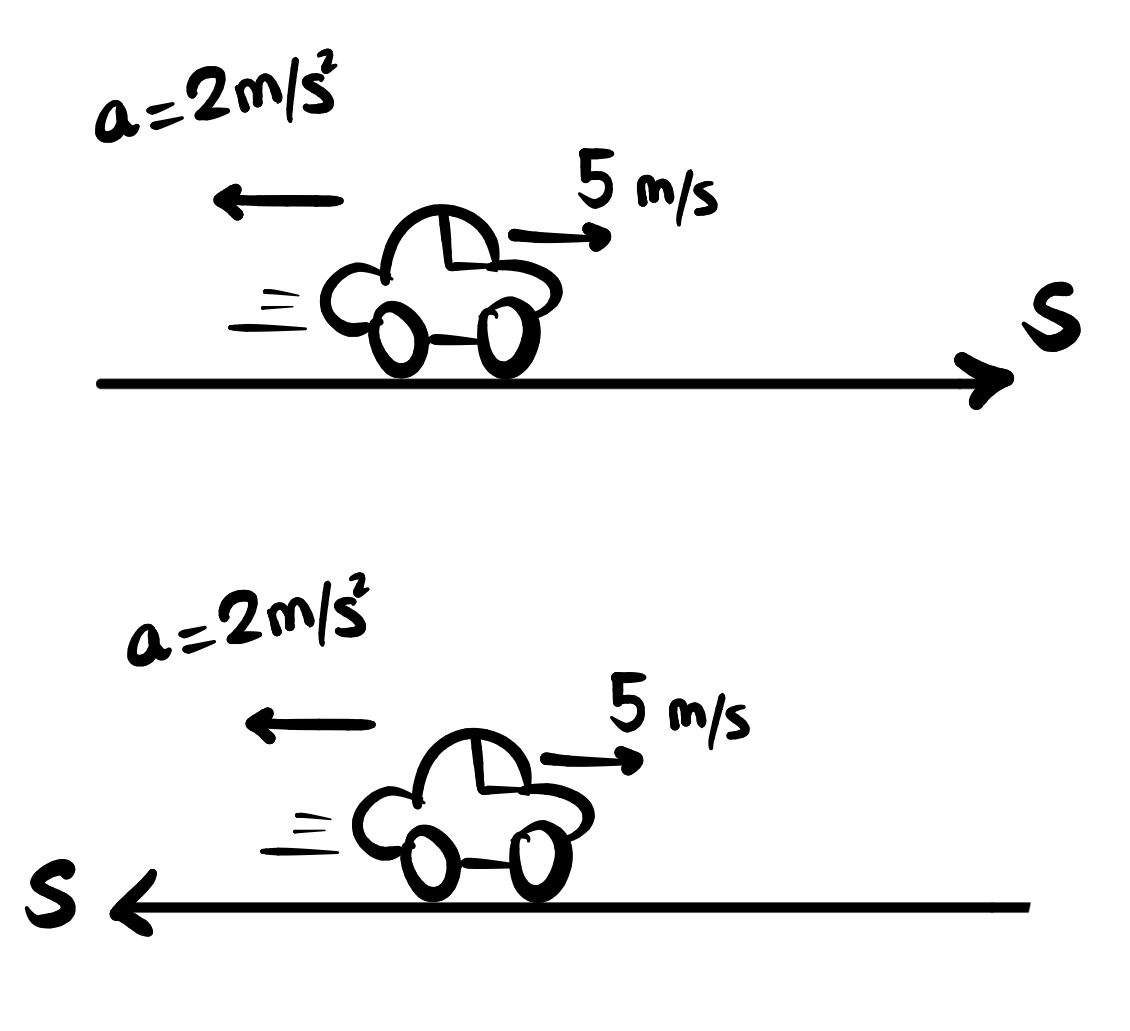
\includegraphics[scale=0.12]{imagensmecanica/muvfuncaovelocidadesinal1.jpeg}
    \caption{Referenciais distintos para equacionar a função da velocidade.}
    \label{fig_mec_muvfuncaovelocidadesinal01}
\end{figure}

Já a mesma equação no referencial da imagem inferior da figura seria diferente: nessa nova escolha de orientação a velocidade inicial é negativa e a aceleração é positiva, de modo que a equação seria:

$$ v(t) = -5+2t,$$
e a velocidade, no mesmo instante $t=5$s, seria $v(5)=5$ m/s. Note que agora a velocidade saiu positiva, o que indica que ela aponta para a esquerda -- uma vez que agora o sentido definido como positivo foi para a esquerda.

Desse modo, usando os dois sistemas de coordenadas distintos, chegamos exatamente à mesma conclusão: a velocidade do carro no quinto segundo de movimento aponta para a esquerda com intensidade de $5$ m/s. É preciso, contudo, saber interpretar os sinais dentro de cada convenção adotada.

Uma observação também merece ser feita a respeito do sinal da aceleração. Um MUV é dito \textbf{acelerado} se a aceleração e velocidade possuem o mesmo sentido, isto é, o mesmo sinal. Isto quer dizer que a velocidade aumenta à medida que o tempo passa. Em contrapartida, o MUV será classificado como \textbf{retardado} caso a velocidade e a aceleração possuam sentidos contrários, ou seja, sinais contrários. Neste caso, o corpo está desacelerando (ou freando), ou seja, ele irá andar cada vez mais devagar até a velocidade zerar.

Dito isso, estudantes costumam se confundir e achar que o movimento será retardado caso a aceleração seja negativa, e acelerado caso ela seja positiva. Note que isso não é verdade, até porque um mesmo movimento pode ter aceleração positiva ou negativa a depender do referencial adotado, como fizemos anteriormente. No primeiro caso a aceleração era positiva e no segundo era negativa -- e o movimento era exatamente o mesmo, só mudamos o sistema de coordenadas usado para descrevê-lo.

Note, portanto, que o que importa para fazer tal tipo de classificação é o sinal da aceleração em relação ao da velocidade: no movimento anterior a velocidade e aceleração sempre possuíam sinais (e portanto sentidos) contrários: inicialmente tínhamos uma velocidade inicial positiva com uma aceleração negativa; ao mudar a orientação passamos a ter uma velocidade inicial negativa e uma aceleração positiva. Nos dois casos os sinais das duas grandezas eram opostos -- indicando que seus sentidos eram opostos -- e, portanto, se velocidade e aceleração possuem sentidos opostos, o movimento é retardado. A Figura \ref{fig_mec_muvfuncaovelocidadestabelasinais} mostra uma tabela com um resumo de todas as possíveis combinações entre os sinais (sentidos) de velocidade e aceleração e o tipo de movimento de cada um deles.

\begin{figure}[h]
    \centering
    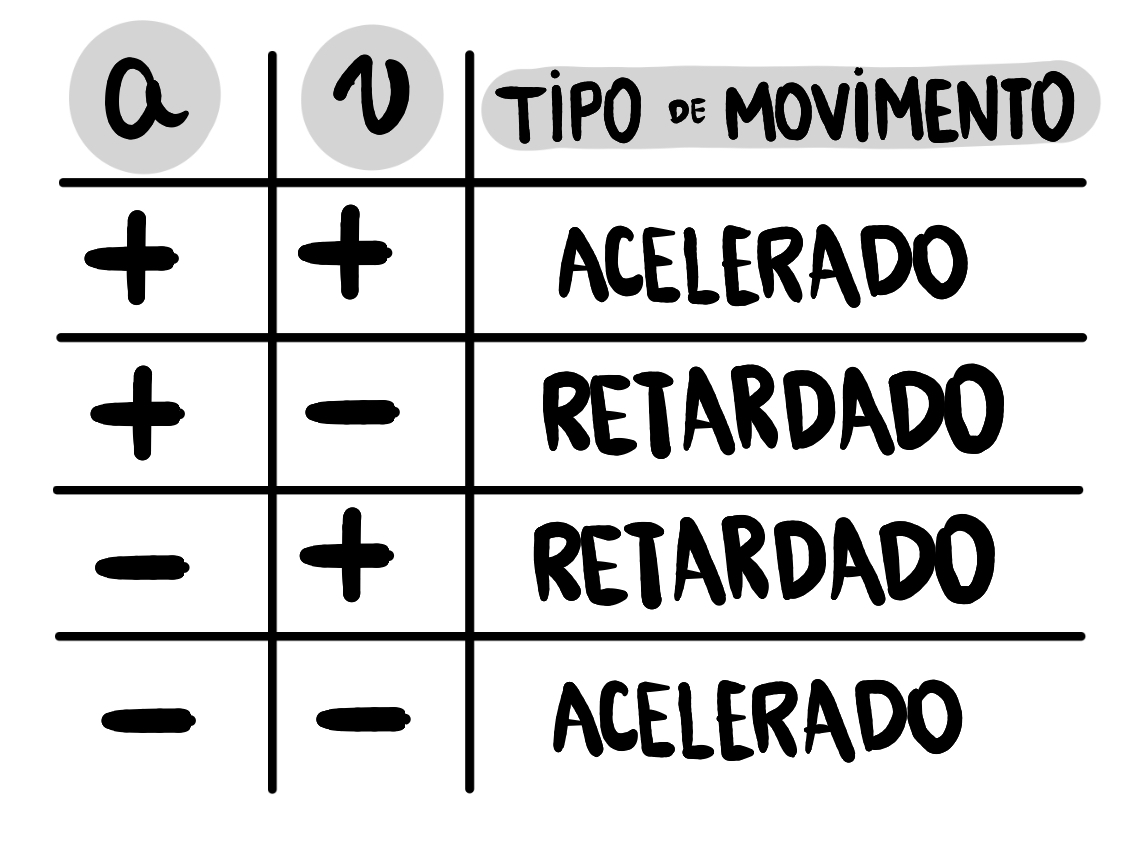
\includegraphics[scale=0.12]{imagensmecanica/muvfuncaovelocidadetabelasinais.jpeg}
    \caption{Classificação do MUV com base na comparação do sentido (sinal) da velocidade e da aceleração.}
    \label{fig_mec_muvfuncaovelocidadestabelasinais}
\end{figure}

%Exemplo resolvido





\vspace{0.3cm}



\begin{exemplo}[Nível I]\label{exemplo_cinematicaescalar_funcaovelocidademuvex01}

Um carro se move com aceleração constante. Sabe-se que, sua velocidade, em um certo instante, é igual a $2$ m/s e, dois segundos após tal instante, a sua velocidade passa a ser de $6$ m/s. Qual é a sua velocidade 10 segundos após ele atingir a velocidade de $6$ m/s?



\resolucao



É interessante fazermos um esboço da situação a fim de não nos perdermos em meio aos dados do problema. Fizemos isso na Figura \ref{fig_mec_funcaovelocidade03}, na qual consideramos o instante inicial do movimento $t_0=0$s como sendo aquele no qual a velocidade vale $2$m/s, que se torna, portanto, a nossa velocidade inicial, ou seja, $v_0 = 2$ m/s.

\vspace{0.3cm}
{
\centering
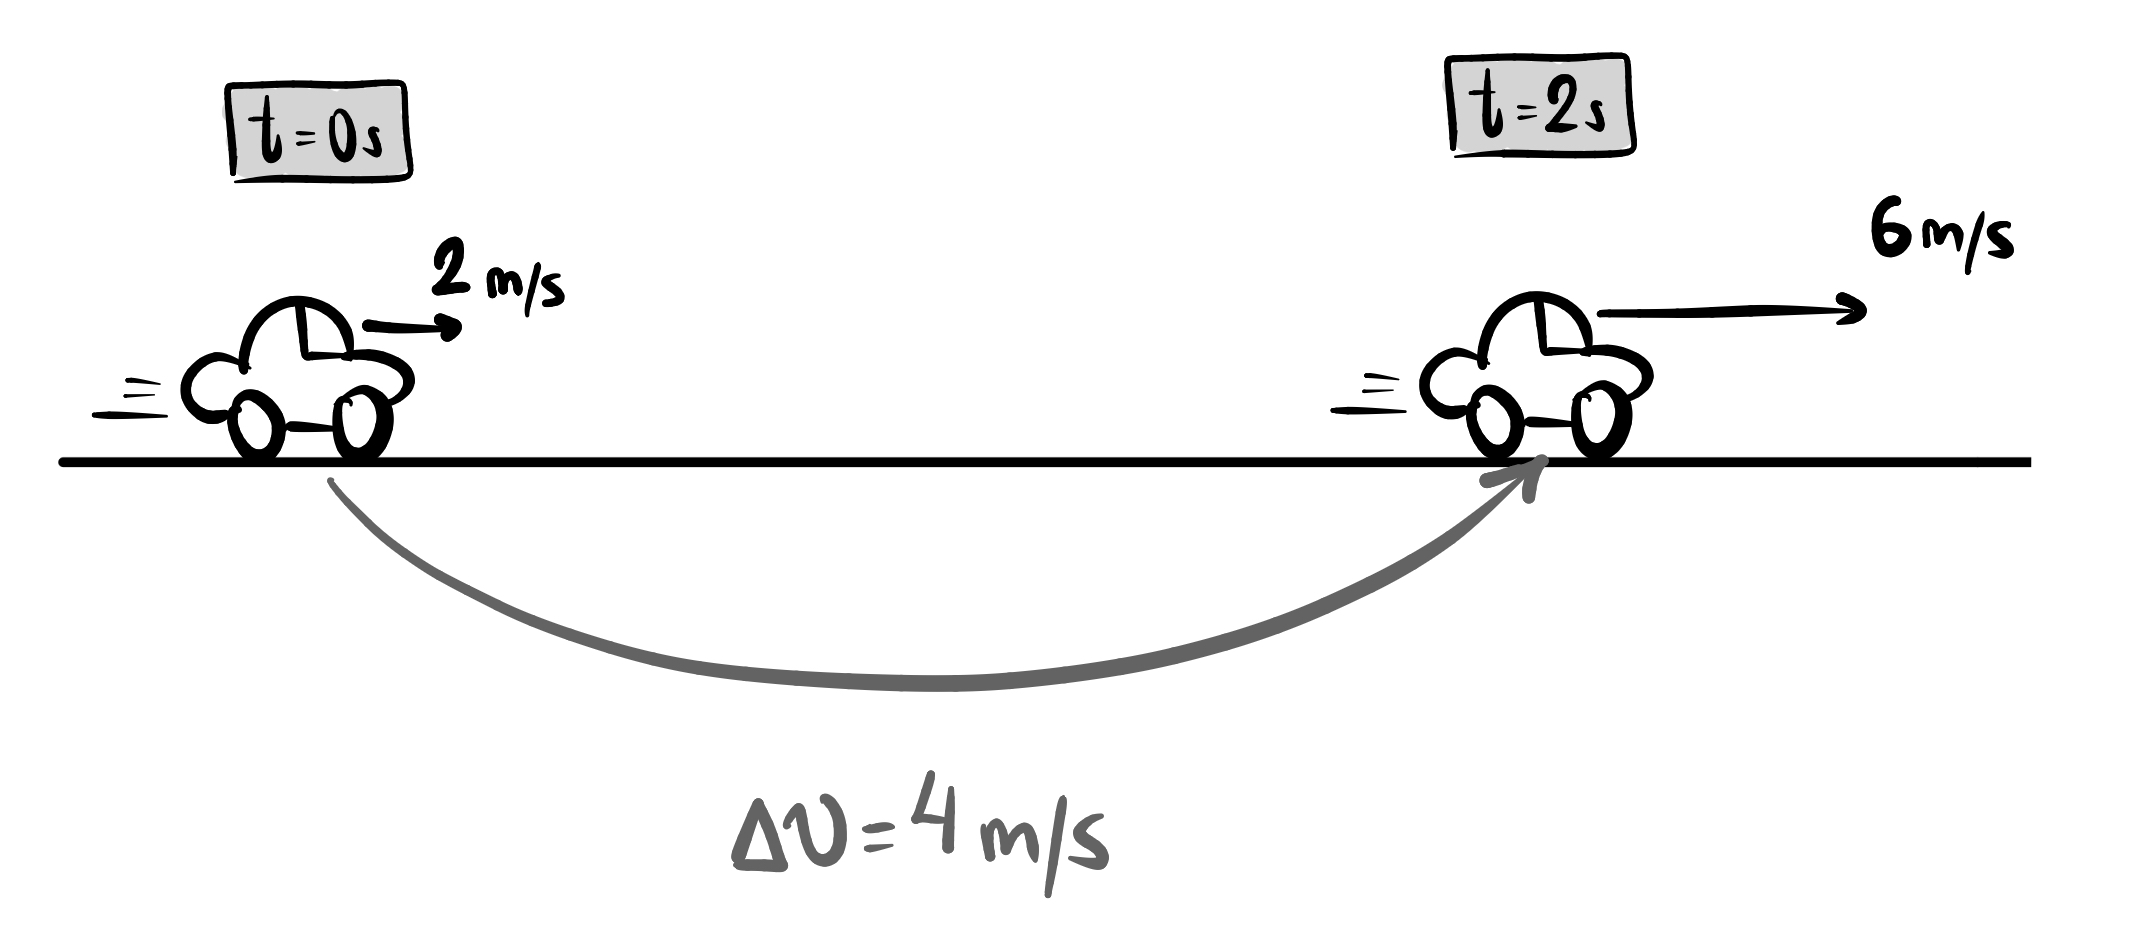
\includegraphics[width=0.5\linewidth]{imagensmecanica/muvfuncaovelocidade03.jpeg}
\captionof{figure}{Referencial orientado para esquerda com origem arbitrária.}
\label{fig_mec_funcaovelocidade03}
} 
\vspace{0.3cm}



Para montar a função horária da velocidade vamos precisar saber qual é a aceleração do carro, o que podemos fazer considerando as informações a respeito dos dois instantes dados:

$$ a = \dfrac{\Delta v}{\Delta t} = \dfrac{6-2}{2-0} = 4 \text{m/s}^2.$$

Munidos de tal valor podemos montar a função horária da velocidade de tal movimento (estamos considerando o sentido positivo para direita):

$$ v = v_0 + at \implies v(t) = 2 + 4t,$$
de modo que agora podemos obter o valor da velocidade $v$ do carro para qualquer instante futuro $t.$ No caso, queremos no instante de tempo 10s após o carro atingir a velocidade de 6 m/s, que é o instante $t=2$s em nossa análise.\footnote{Lembre-se de que o instante inicial $t_0=0$s é aquele no qual a velocidade é $v_0$, o qual consideramos sendo a velocidade de 2 m/s, e não 6 m/s. } Assim, 10s após isso, estaremos no instante $t=12$s, de modo que a velocidade em tal momento é dada por 
$$v(12)=2+4\cdot12 = \boxed{50 \text{m/s}.}$$

\end{exemplo}






\vspace{0.3cm}





\begin{exemplo}[Nível II]\label{exemplo_cinematicaescalar_funcaovelocidademuvex02}




Considere uma bola, lançada verticalmente para cima, em $t=0$, com velocidade de $30$ m/s. Se a aceleração da gravidade é igual a $10$ m/s$^2$, calcule:

\begin{enumerate}
    \item [(a)] O instante de tempo no qual a bola inverte o sentido do movimento.
    \item [(b)] A velocidade da bola em $t=5$s.
\end{enumerate}


\resolucao


\begin{enumerate}
    \item [(a)] O instante de tempo no qual um corpo em MUV inverte o sentido do movimento sempre será aquele no qual a velocidade é $0.$ Isso porque, se o corpo está sendo desacelerado, ele o será até que sua velocidade seja totalmente diminuída, ou seja, ela chegue em zero. Daí em diante, caso a mesma aceleração que o freou permaneça atuando, ela começará a acelerar o corpo no sentido contrário ao qual ele se movia -- a mesma aceleração gera, agora, um movimento acelerado, e não mais retardado.

    Logo, a bola chegará no ponto de altura máxima -- posição em que sua velocidade zera -- e inverterá seu sentido do movimento quando

    $$ v(t) = v_0+at =0\implies v(t) = 30-10t =0 \implies \boxed{t=3 \text{ s,}}  $$

    \noindent em que consideramos um sistema de coordenadas orientado para cima.


    
    \item [(b)] Alguns leitores poderiam pensar que é preciso construir uma nova função horária da velocidade após $t=3$s, haja vista que agora o movimento se dá em um sentido contrário, e deixou de ser retardado para ser acelerado.

    Isso é um equívoco, e tal construção é totalmente desnecessária. O fato de que o movimento mudou de sentido já é capturado pela função horária da velocidade por meio do sinal: no sistema que adotamos, orientado para cima, velocidades para cima são positivas e velocidades para baixo são negativas. 

    Logo, note que, quando o corpo começa a cair, sua velocidade ficará negativa -- a própria equação já conterá essa informação -- e, sendo a aceleração da gravidade negativa (uma vez que ela está orientada para baixo) teremos a velocidade e a aceleração com mesmo sinal, isto é, mesmo sentido, o que já captura informação de que o movimento passou a ser acelerado. 

    Portanto, para qualquer instante de tempo podemos usar a mesma equação $v(t)=30-10t,$ de modo que, em $t=5$s, teremos:

    $$ v(5)=30-10\cdot 5 \implies v(5)=-20 \text{ m/s},$$

    \noindent o que quer dizer uma velocidade com valor de $20$ m/s orientada para baixo. Veja que isso é condizente com o esperado: após $t=3$s quaisquer velocidades informadas pela equação devem ser negativas, uma vez que o sentido do movimento se inverte naquele instante.

    
\end{enumerate}

\end{exemplo}




\vspace{0.3cm}



% \begin{exemplo}[Nível III]\label{exemplo_cinematicaescalar_funcaovelocidademuvex03}



% \resolucao


% \end{exemplo}






% \vspace{0.3cm}






\begin{secnivel}[Função Horária da Posição do MUV]{I}{Função Horária da Posição do Movimento Uniformemente Variado}
 

  \eqLdois{dem}{mecanica_eq_muvfuncaoposicao}{\Delta s = v_0t + \dfrac{1}{2}at^2 \quad \text{ou} \quad  s = s_0+v_0t + \dfrac{1}{2}at^2 }
  
\end{secnivel}








\secgfe{De onde vem}

Antes de dar sequência a essa demonstração, é importante que o leitor tenha passado com calma e compreendido por completo o conteúdo do Apêndice \ref{apendice_areagraficovxt}. Feito isso, para demonstrar tal equação usaremos justamente o fato de que a área abaixo do gráfico de velocidade por tempo fornece o deslocamento $\Delta s$ do corpo naquele intervalo de tempo. 

Para o MUV, sabemos que a velocidade varia no tempo de acordo com a Equação \eqref{mecanica_eq_muvfuncaovelocidade}, que é uma função afim, cujo gráfico é uma reta. Tal reta se encontra representada na Figura \ref{fig_mec_graficovxt}, na qual usamos, novamente, a Equação \eqref{mecanica_eq_muvfuncaovelocidade} para marcar que a velocidade da partícula no instante $t$ será $(v_0+at).$

\begin{figure}[h]
    \centering
    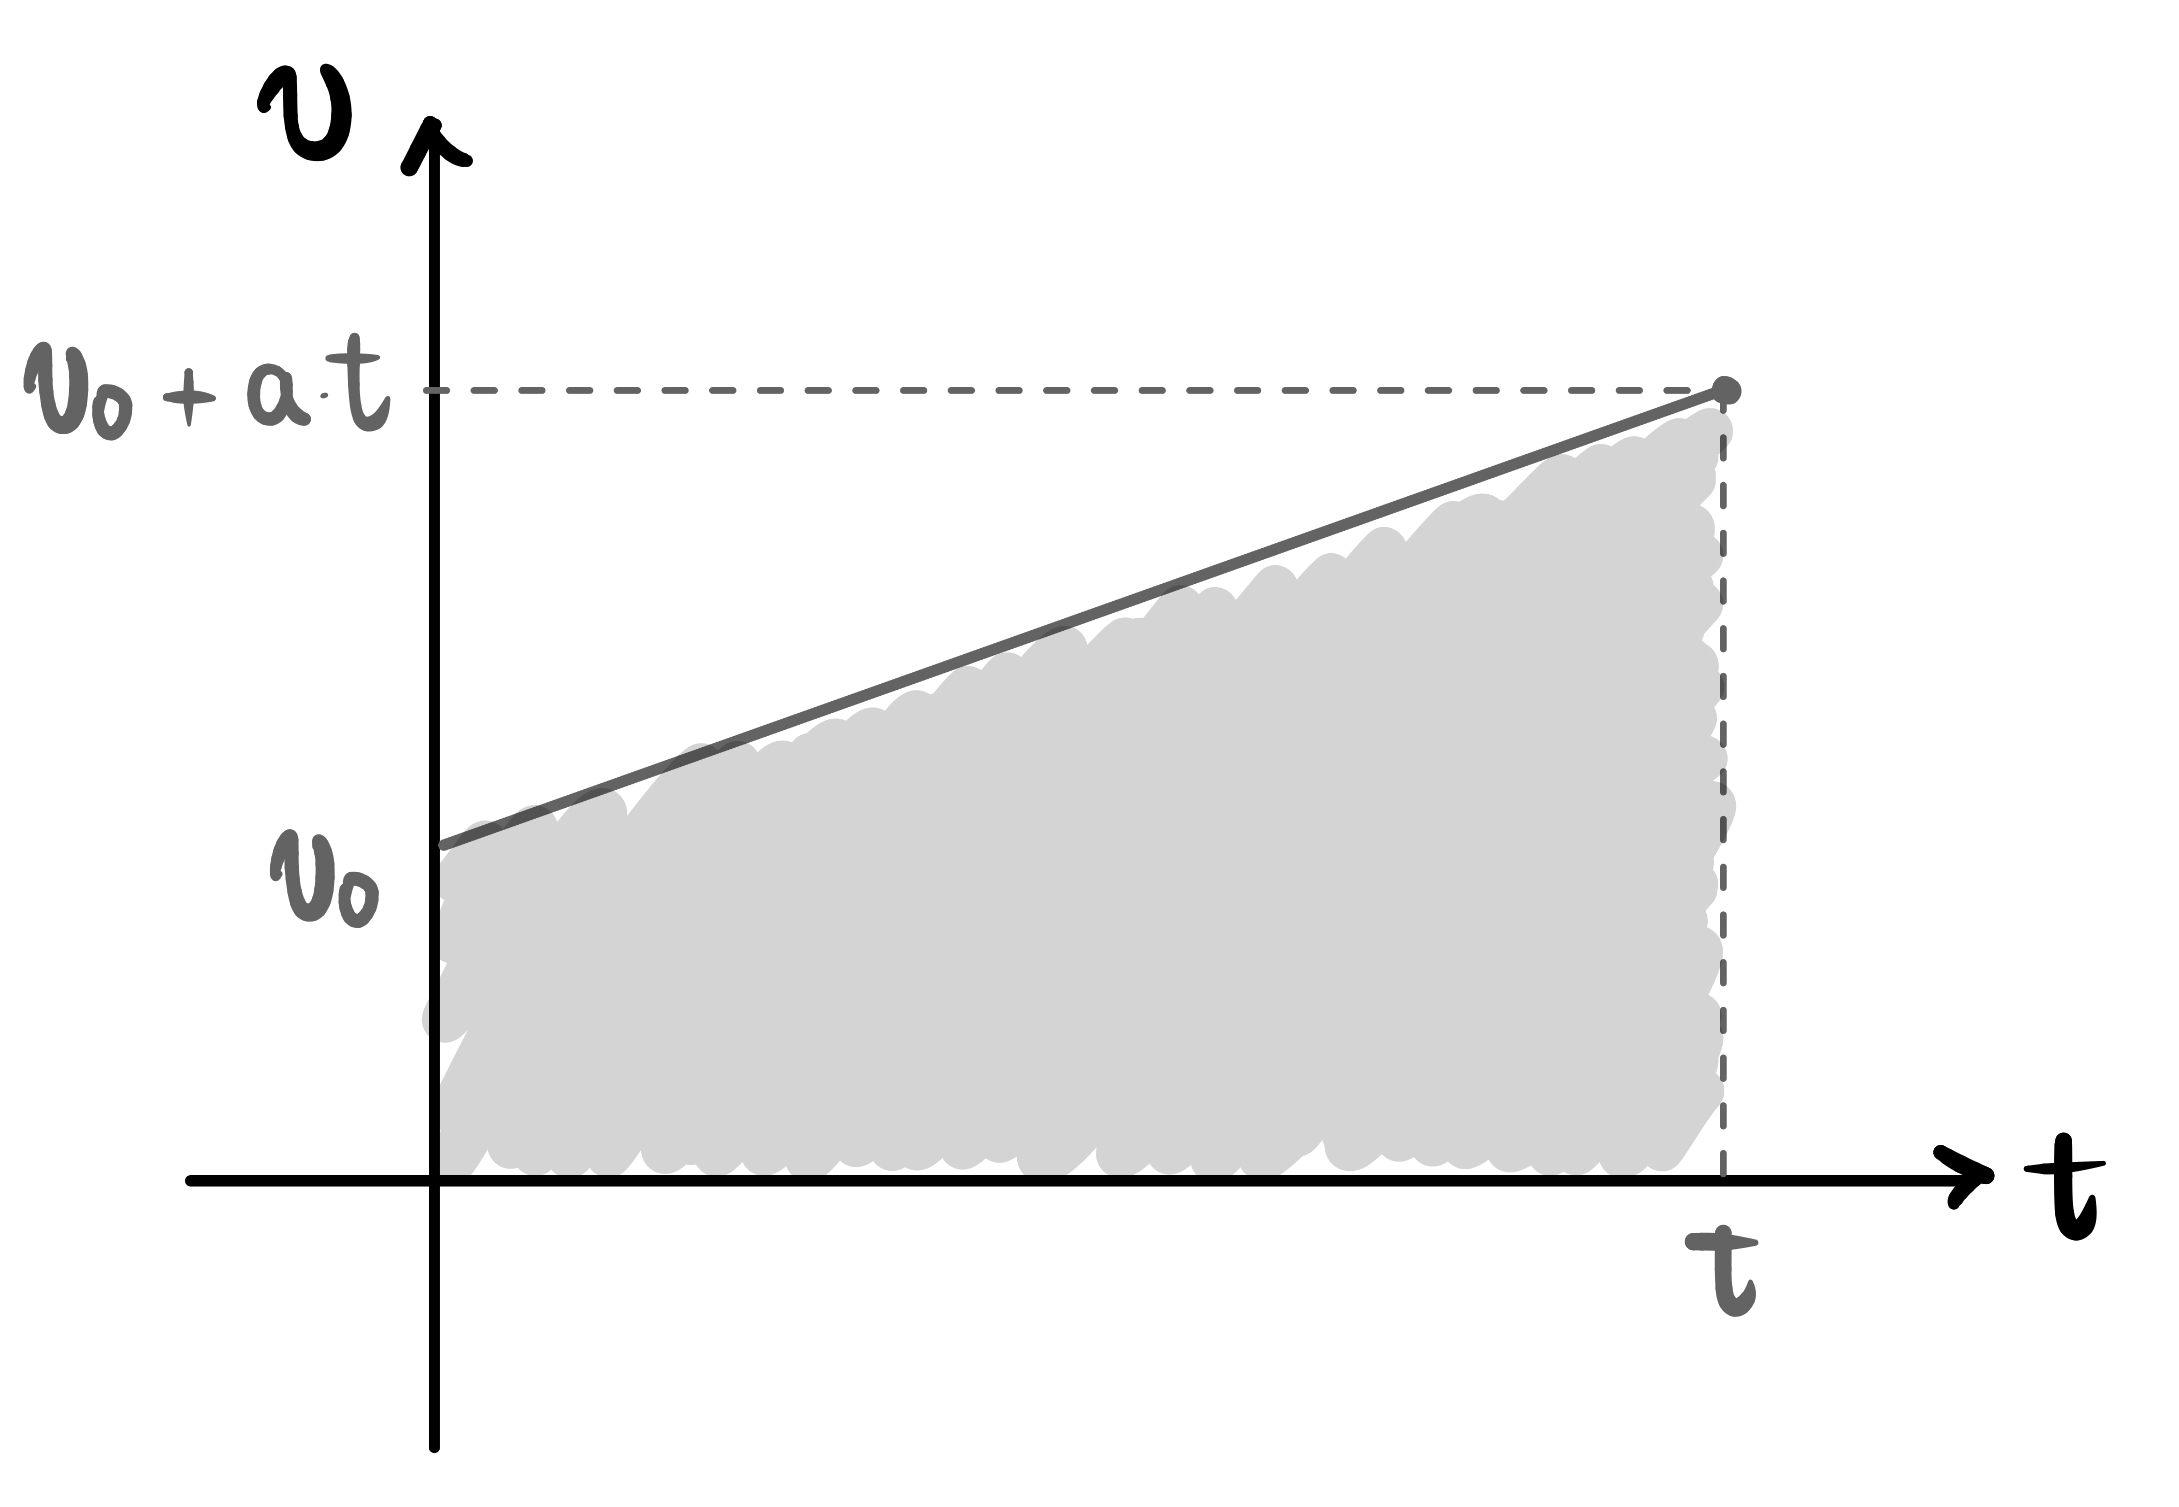
\includegraphics[scale=0.09]{imagensmecanica/muvgraficovxt.jpeg}
    \caption{Gráfico $v$ por $t$ para o MUV. }
    \label{fig_mec_graficovxt}
\end{figure}

O deslocamento da partícula no intervalo de $0$ a $t$ será, portanto, a área abaixo do gráfico ao longo deste intervalo, que incorre em ser a área de um trapézio, de altura $t$ e bases $v_0$ e $(v_0+at),$ sendo sua área $A$ dada por

$$ A=\Delta s = \dfrac{(B+b)\cdot h}{2}= \dfrac{(v_0+(v_0+at))\cdot t}{2} = \dfrac{2v_0t+at^2}{2} \implies \boxed{\Delta s = v_0t + \dfrac{1}{2}at^2.} $$

Sendo o deslocamento $\Delta s$ igual à variação da posição, isto é, sendo $s$ a posição da partícula no instante $t$ e $s_0$ sua posição no instante inicial $t=0$s, temos que $\Delta s = (s-s_0),$ de modo que a equação acima pode ser escrita como

$$ s=s_0+ v_0t + \dfrac{1}{2}at^2.$$

A Equação \eqref{mecanica_eq_muvfuncaoposicao} é o análogo da Equação \eqref{mecanica_eq_mu_funcaoposicao}, porém essa descreve a evolução da posição no Movimento Uniforme, enquanto aquela descreve como a posição evolui no Movimento Uniformemente Variado.\footnote{Note, inclusive, que ao tornar a aceleração nula na Equação \eqref{mecanica_eq_muvfuncaoposicao}, desaguamos justamente na função horária da posição do MU -- na qual $v_0=v$, haja vista que a velocidade é constate e nunca muda. Isso tem a ver com  fato anteriormente discutido de que o MU é um caso particular do MUV para o qual a aceleração tem o específico valor zero.}

\secgfe{Onde é usada}

Em qualquer contexto que se deseje computar a distância percorrida ou estudar a evolução das posições de um objeto que se move com aceleração constante. Considere, por exemplo, um carro que se move com aceleração de 6 m/s$^2$, que aponta no mesmo sentido da sua velocidade, que, inicialmente, é de 10 m/s. Se a posição inicial deste carro é no quilômetro 40 de uma rodovia, qual será a sua posição após 15 minutos de viagem?

Montando a função horária da posição para tal movimento, teremos (atente-se às unidades de medida):

$$ s(t)=s_0+v_0t +\dfrac{1}{2}at^2 \implies s(t)=40.000+10t+3t^2.$$

Note que tal equação nos possibilita descobrir aonde o carro estará, isto é, qual é a sua posição $s(t)$, para qualquer instante de $t$ futuro. Em particular, após 15 minutos, que são $15*60=900$ segundos, a posição do carro será

$$s(900)= 40.000+10\cdot 900+3 \cdot 900^2 \implies \boxed{ s(900)=2.479.000 \text{m}=2.479 \text{km},}$$
ou seja, o carro estará para lá do quilômetro dois mil da rodovia.\footnote{Caso o leitor tenha achado tal número estranho, reitero que ele é factível -- pelo menos em termos da geografia do Brasil. A BR-116, que conecta Fortaleza ao Rio Grande do Sul, possui cerca de 4.600 km de extensão. Contudo, certamente é impossível percorrê-la em 15 ou 30 minutos, de carro. O que acontece é que uma aceleração de 6 m/s$^2$, apesar de ser possível para um carro, não pode jamais ser mantida por 15 minutos. Com tal valor de aceleração, um carro vai de 0 a 100 km/h em cerca de 5 segundos. Logo, se ele conseguisse manter essa aceleração pelos próximos 14 minutos e 55 segundos seguintes, ele alcançaria uma velocidade de quase 20 mil km/h, o que certamente o leitor nunca deve ter visto acontecendo por aí. }



\secgfe{Erros comuns}

O erro mais comum aqui é o estudante usar a função horária da posição do MU quando o movimento é acelerado. Ou seja, é como se ele acabasse esquecendo para trás o fator $\sfrac{at^2}{2}.$

É importante notar que as Equações \eqref{mecanica_eq_mu_funcaoposicao} e \eqref{mecanica_eq_muvfuncaoposicao} de fato guardam similaridades: as duas se propõem a fazer a mesma coisa -- dizer como a posição de um corpo evolui no tempo ao longo de seu movimento. Contudo, elas o fazem para movimentos distintos: uma delas é para o movimento com velocidade constante, a outra para o movimento com aceleração constante. Movimentos de natureza e características distintas, naturalmente, terão equações diferentes para descrever sua evolução.

\secgfe{Observações}


É importante notar que a Equação \eqref{mecanica_eq_muvfuncaoposicao}, em seu primeiro formato, calcula o deslocamento do corpo, e não a distância percorrida. Para deixar isso claro, considere um corpo em um MUV em que sua velocidade inicial é de $30$ m/s e sua aceleração é de $10$ m/s$^2$, contrária ao sentido da velocidade inicial. Pede-se calcular a distância percorrida por tal corpo ao longo dos primeiros 6 segundos de movimento.

O estudante mais desavisado poderia escrever que

$$ d=v_0t+\dfrac{1}{2}at^2 \implies d = 30t+\dfrac{1}{2}(-10)t^2 \implies d=30 \cdot 6 -5 \cdot 6^2 \implies \boxed{d=0\text{m}.}$$

Como pode um corpo estar se movendo -- de forma acelerada, inclusive --  percorrer uma distância nula? Naturalmente, tal resultado está errado. E o erro foi em considerar que deslocamento $\Delta s$ é igual à distância percorrida. Novamente, note que a Equação \eqref{mecanica_eq_muvfuncaoposicao} fornece o \textbf{deslocamento} do corpo em MUV, e \textbf{não a distância que ele percorre}. Ou seja, o que calculamos acima, na verdade, é que $\Delta s=0$m, o que não é incoerente com o tipo de movimento. O que isso quer dizer é que o corpo, no sexto segundo de movimento, retorna para a mesma posição em que ele estava quando o movimento iniciou.

Isso não é incoerente porque o movimento, inicialmente, é retardado: a aceleração é contrária à velocidade. Isso quer dizer que o nosso objeto terá sua velocidade diminuída até zerar. Caso a aceleração continue existindo, ela irá, a partir do momento em que a velocidade zera, começar a fazer o objeto ganhar movimento no sentido oposto, ou seja, o objeto começa a ``voltar'', de modo que, em algum momento, ele passará de volta pela sua posição inicial. Neste instante, seu deslocamento total é nulo -- a posição inicial e final são iguais.

Tal situação -- que é justamente a do problema -- está descrita na Figura \ref{fig_mec_muvlancamentovertical}. Note que, ao longo dos primeiros 3 segundos de movimento, a velocidade vai de $30$ m/s a $0$ m/s. Daí em diante, o movimento é simétrico: o corpo inverte o sentido do seu movimento e a velocidade agora vai de $0$ m/s a $30$ m/s -- o sinal negativo só indica que, agora, o sentido do movimento inverteu. Assim, nos primeiros 6 segundos de movimento, o objeto sobe, atinge a altura máxima e retorna à mesma posição inicial, de modo que o deslocamento total é nulo. Essa é a exata experiência que o leitor pode ter ao lançar verticalmente para cima uma pedra.

\begin{figure}[h]
    \centering
    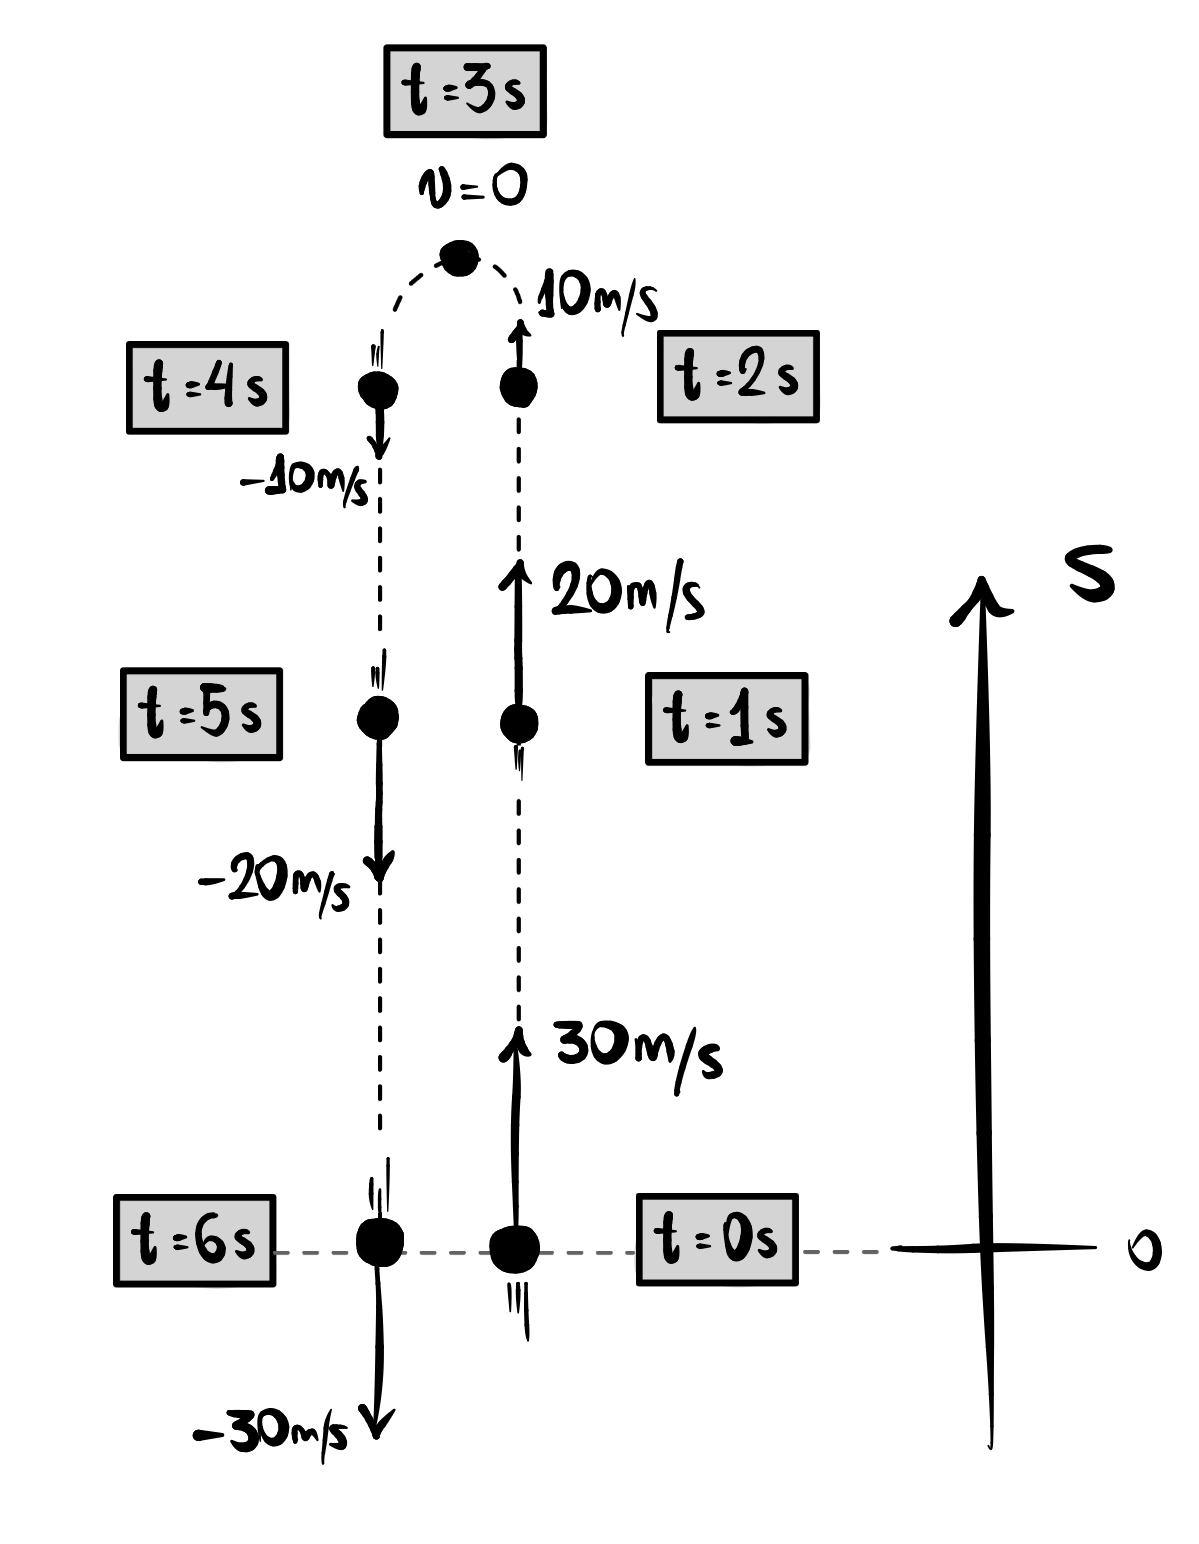
\includegraphics[scale=0.18]{imagensmecanica/muvfuncaoposicaoexemplo.jpeg}
    \caption{O lançamento vertical de uma pedra e o deslocamento total nulo.}
    \label{fig_mec_muvlancamentovertical}
\end{figure}

Como poderíamos perceber e computar tudo isso, sem o auxílio da Figura \ref{fig_mec_muvlancamentovertical}? Perceba que, em qualquer movimento retardado, este é um cuidado que o leitor deverá tomar. Porque em um movimento acelerado o sentido do movimento nunca muda, de modo que a distância sempre coincidirá com o deslocamento, e o raciocínio feito anteriormente estaria sempre correto.

Contudo, em um movimento retardado, eventualmente o sentido do movimento pode mudar, de modo que distância e deslocamento deixarão de coincidir, e é aí onde deve-se tomar cuidado. Para saber se isso ocorreu, é preciso descobrir quando a velocidade zera, porque é a partir daí que o sentido do movimento irá inverter. Para o movimento do exemplo, começamos com $v_0= 30$ m/s e $a=-10 $ m/s$^2$ (estamos considerando o sentido positivo como sendo aquele para onde aponta a velocidade inicial). Neste caso, a função horária da velocidade -- Equação \eqref{mecanica_eq_muvfuncaovelocidade} -- de tal movimento é

$$ v(t)=v_0+at \implies v(t) = 30 - 10t.$$

Queremos saber em qual instante a velocidade zera, isto é:

$$v(t)=30-10t =0 \implies \boxed{t=3\text{s.}}$$


Ora, acabamos de descobrir que a velocidade zera no terceiro segundo de movimento. Isso quer dizer que, nos primeiros 3 segundos de movimento, distância e deslocamento coincidem: o movimento se dá ao longo de um mesmo sentido (a Figura \ref{fig_mec_muvlancamentovertical} evidencia isso). Daí em diante o sentido do movimento irá inverter, e a distância e o deslocamento deixarão de coincidir. Sendo assim, a fim de computar a distância total percorrida por tal objeto nos primeiros 6 segundos de movimento, teríamos que calcular primeiro o seu deslocamento ao longo dos três primeiros segundos -- porque ele coincide com a distância -- e depois seu deslocamento do segundo 3 ao segundo 6, que também coincidirá com a distância neste intervalo.

Para os primeiros 3 segundos teríamos:

$$d_1=\Delta s_1=v_0t+\dfrac{1}{2}at^2 \implies d_1 = 30t +\dfrac{1}{2}(-10)t^2 \implies d_1 =30\cdot 3 -5 \cdot 3^2 \implies \boxed{d_1=45\text{m}.}$$


A partir de agora, teríamos que computar o deslocamento nos 3 segundos subsequentes. Contudo, percebendo que o movimento é simétrico -- a distância percorrida na subida, nos primeiros 3 segundos, é igual à distância percorrida na descida, nos próximos 3 segundos -- poderíamos de imediato concluir que a distância total percorrida é o dobro do valor anteriormente calculado, isto é $D=2d_1= \boxed{90 \text{m}.}$

\begin{figure}[h]
    \centering
    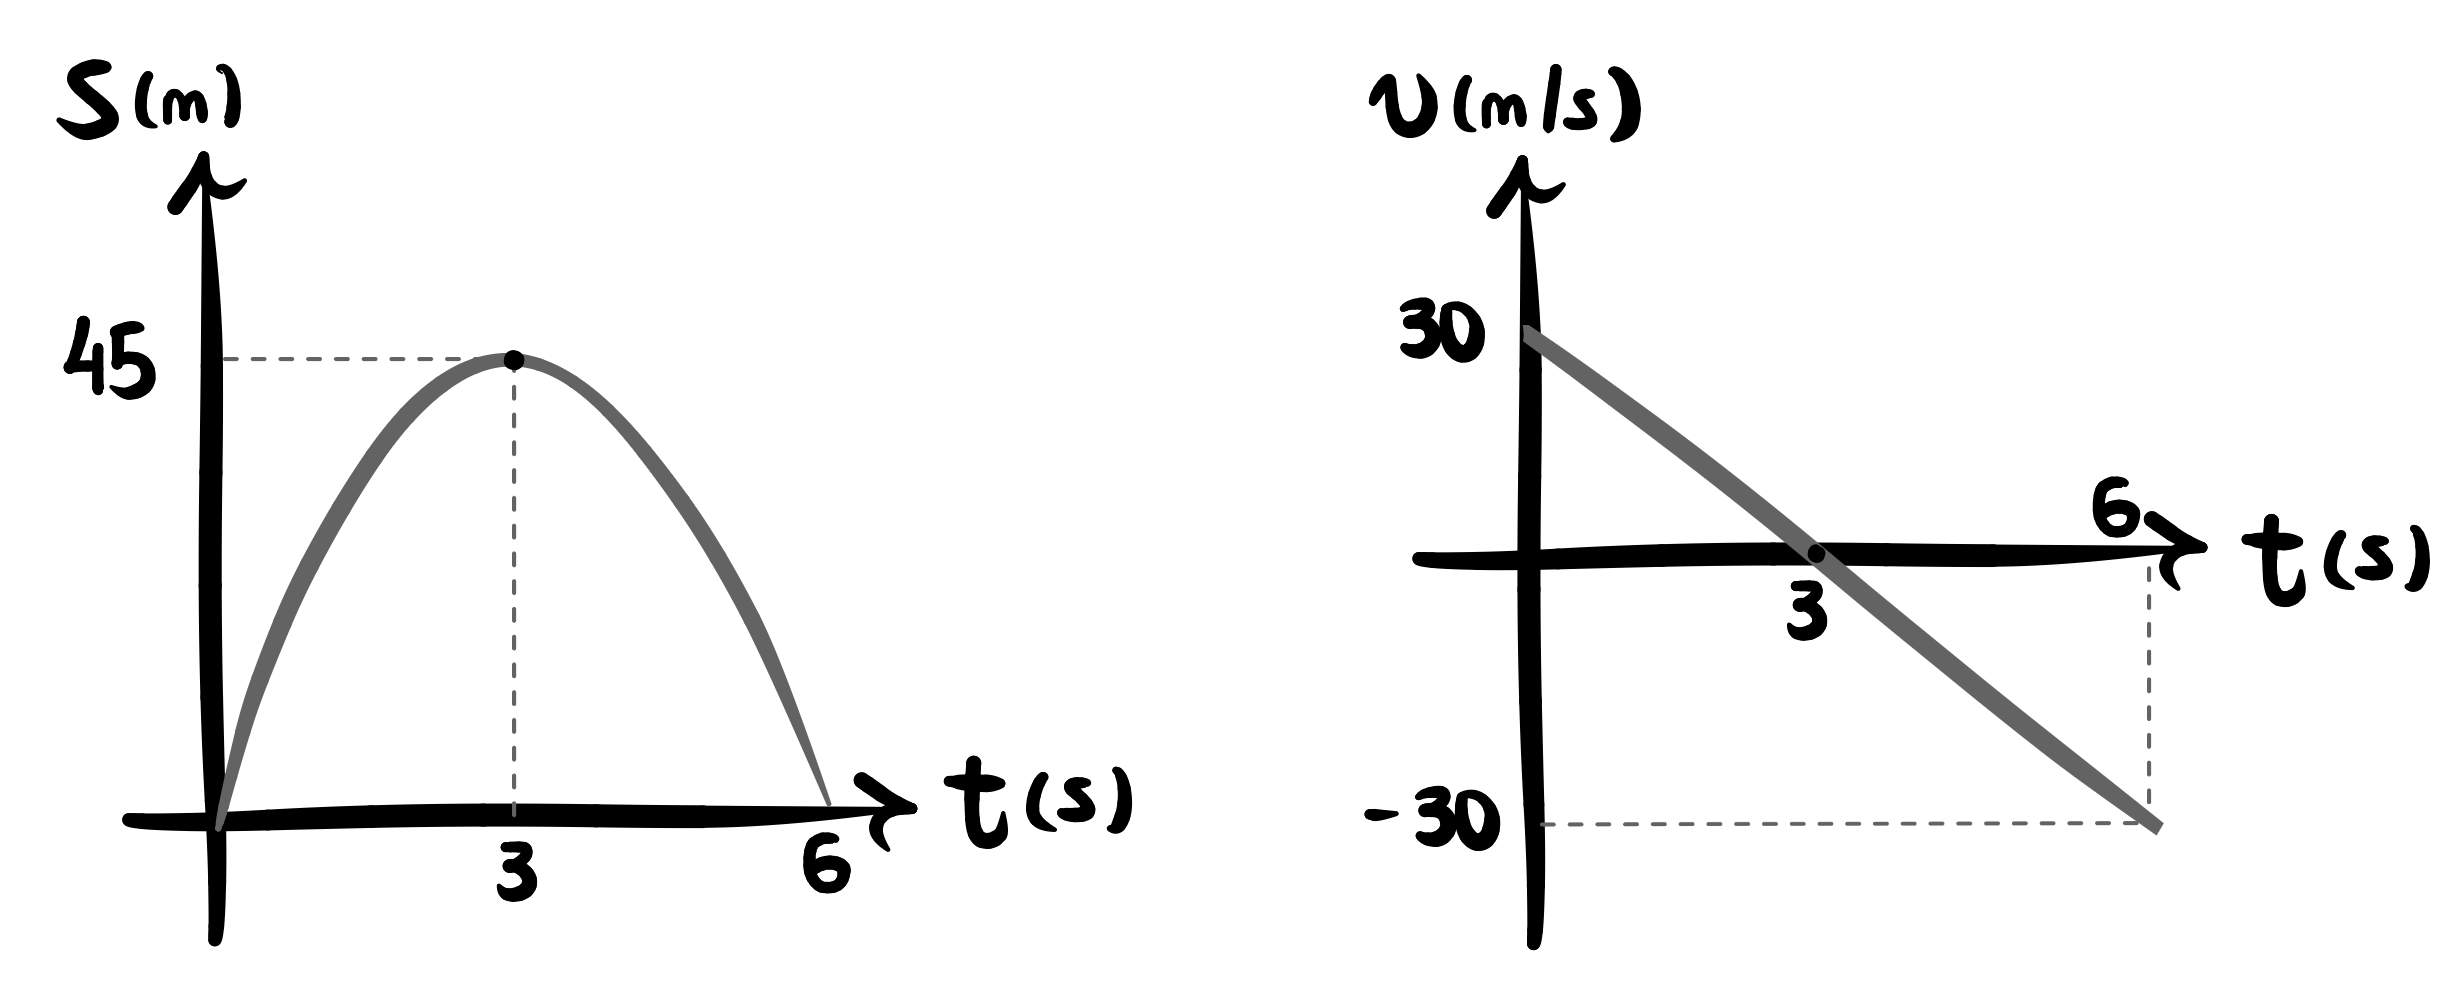
\includegraphics[scale=0.28]{imagensmecanica/graficosmuv.png}
    \caption{Os gráficos de posição e velocidade por tempo do movimento da pedra da Figura \ref{fig_mec_muvlancamentovertical}.}
    \label{fig_mec_graficosmuv}
\end{figure}

A Figura \ref{fig_mec_graficosmuv} mostra os gráficos de posição e velocidade por tempo, respectivamente, do movimento da pedra. Note, no gráfico de posição por tempo, que a posição aumenta até o terceiro segundo -- ponto em que a posição (altura) da pedra é máxima -- e passa a regredir deste instante em diante. Ou seja, o sentido do seu movimento deve inverter a partir de $t=3$s. O gráfico da direita, da velocidade por tempo, é compatível com isso: a velocidade é positiva nos primeiros 3 segundos, zerando em $t=3$s e se tornando negativa daí em diante. A inversão do sinal da velocidade indica a inversão no sentido do movimento.

%Exemplo resolvido

\vspace{0.3cm}

\begin{exemplo}[Nível I]\label{exemplo_cinematicaescalar_funcaoposicaomuvex01}


Uma câmera eletrônica está instalada em $s=0$ em uma certa avenida. Um carro passa por este ponto no instante $t=0,$ com velocidade de 15 m/s. A partir desse instante, o carro passa a acelerar uniformemente com aceleração de $2$m/s$^2$.

\begin{itemize}
    \item [(a)] Qual é a posição do carro após 10s?
    \item [(b)] Em qual instante o carro atinge a posição $s=1$km?
\end{itemize}



\resolucao



Convencionemos que o sentido positivo é aquele para o qual aponta a velocidade do carro. Neste caso, a função horária da posição do seu movimento é dada por

$$ s= s_0+v_0t+\dfrac{1}{2}at^2 \implies \boxed{ s(t)=15t+t^2.}$$

\begin{itemize}
    \item [(a)] Em $t=10$s a posição do carro será dada por:
    $$ s(10)=15 \cdot 10 + 10^2 = \boxed{250 \text{m}.}$$

    \item [(b)] Para saber em qual instante de tempo o carro alcança a posição $s=1000$m precisamos resolver a equação:

    $$ s(t)= 15t+t^2 = 1000 \implies t^2+15t-1000=0,$$
    cujas soluções são $t_1=-40$s e $t_2=25$s. Descartamos, naturalmente, a primeira solução, por ser negativa e não ter sentido físico. Assim, o carro atinge a posição $s=1$km em \boxed{$t=25$ \text{s}.}
\end{itemize}

\end{exemplo}


\vspace{0.3cm}





\begin{exemplo}[Nível II (ITA 2016)]\label{exemplo_cinematicaescalar_funcaoposicaomuvex02}


A partir do repouso, um foguete de brinquedo é lançado verticalmente do chão,
mantendo uma aceleração constante de $5{,}00\ \text{m/s}^2$ durante os
$10{,}0$ primeiros segundos. Desprezando a resistência do ar, a altura máxima
atingida pelo foguete e o tempo total de sua permanência no ar são,
respectivamente, de

\begin{enumerate}
  \item [(a)] $375\ \text{m}$ e $23{,}7\ \text{s}$
  \item [(b)] $375\ \text{m}$ e $30{,}0\ \text{s}$
  \item [(c)] $375\ \text{m}$ e $34{,}1\ \text{s}$
  \item [(d)] $500\ \text{m}$ e $23{,}7\ \text{s}$
  \item [(e)] $500\ \text{m}$ e $34{,}1\ \text{s}$
\end{enumerate}

\resolucao



Vamos dividir o estudo do movimento em duas partes:

\begin{enumerate}
    \item [(i)] Primeiros 10 segundos de movimento.

  Considere um sistema de coordenadas com origem na posição inicial do foguete, no chão, e com orientação para cima. Assim, a função horária da posição do foguete é
  $$ s= \cancelto{0}{s_0}+\cancelto{0}{v_0}+\dfrac{1}{2}5t^2 \implies \boxed{s(t)=\dfrac{5}{2}t^2.}$$

  Após 10 segundos sua posição será, naturalmente, $s(10)= \sfrac{5}{2}\cdot 10^2 = 250$m. Já a função horária da velocidade do foguete é

  $$ v= \cancelto{0}{v_0}+at \implies \boxed{v(t)=5t,}$$

  \noindent de modo que sua velocidade, em $t=10$s, é $v(10)=5\cdot 10=50$ m/s.

  \item[(ii)] Consideramos o movimento a partir de $t=10$s, no qual o foguete desligou sua aceleração. A partir de agora, é como se tivéssemos um lançamento vertical para cima, com velocidade inicial de $50$ m/s e sendo desacelerado pela gravidade, com aceleração de $g=10$m/s$^2.$ A função horária da velocidade é

  $$ v(t')=v_0+at' \implies \boxed{v(t')=50-10t',}$$

 \noindent e sua função horária da posição é

 $$s(t') = s_0 + v_0t'+ \dfrac{1}{2}at'^2 \implies \boxed{s(t')=250+50t'-5t'^2.}$$

 Perceba que estamos usando o mesmo referencial: orientado para cima e com origem no chão -- é por isso que agora a posição inicial do objeto é $s_0=250$m. O que mudamos foi apenas o tempo: é como se tivéssemos, a partir do ponto no qual o foguete está na posição $s=250$m, soltado um novo cronômetro, que marca o tempo $t'.$ É importante destacar essa diferença porque este tempo $t'$ está 10 segundos atrás do nosso tempo $t$ inicial, ou seja, $t'=t-10.$ Logo, quando $t=10$s, teremos $t'=0,$ que é a situação a partir da qual começaremos a equacionar. Dito isso, queremos que o foguete retorne ao chão, ou seja, sua posição final deve voltar a ser $s=0:$

 $$ s(t')=250+50t'-5t'^2=0 \implies \boxed{t'=5\pm5\sqrt3.}$$

 Uma das soluções da equação quadrática é negativa, de modo que a desprezamos. Assim, o instante de tempo até que o foguete retorne ao solo é $t'=5+5\sqrt3 \approx 13,65$ segundos. Logo, como $t'=t-10,$ segue que o tempo total, a partir do lançamento do foguete, até que ele retorne ao solo, é

 $$ t = t'+ 10 = 13,65 + 10 \implies \boxed{t=23,65 \text{ segundos.}} $$

 A altura máxima ocorrerá quando a velocidade tiver zerado, ou seja:

 $$ v(t')=50-10t' = 0 \implies \boxed{t'=5 \text{ segundos,}}$$

\noindent instante no qual a posição do foguete será

$$ s(t')=250+50t'-5t'^2 \implies s(5)=250+50 \cdot 5 -5 \cdot 5^2 \implies \boxed{ s(5)= 375 \text{ metros,}} $$

 \noindent de modo que a letra A fica sendo a resposta.
    
\end{enumerate}

  

\end{exemplo}

\vspace{0.3cm}





\begin{exemplo}[Nível III (ITA 2003)]\label{exemplo_cinematicaescalar_funcaoposicaomuvex03}

A partir do repouso, uma pedra é deixada cair da borda no alto de um edifício. 

{
\centering
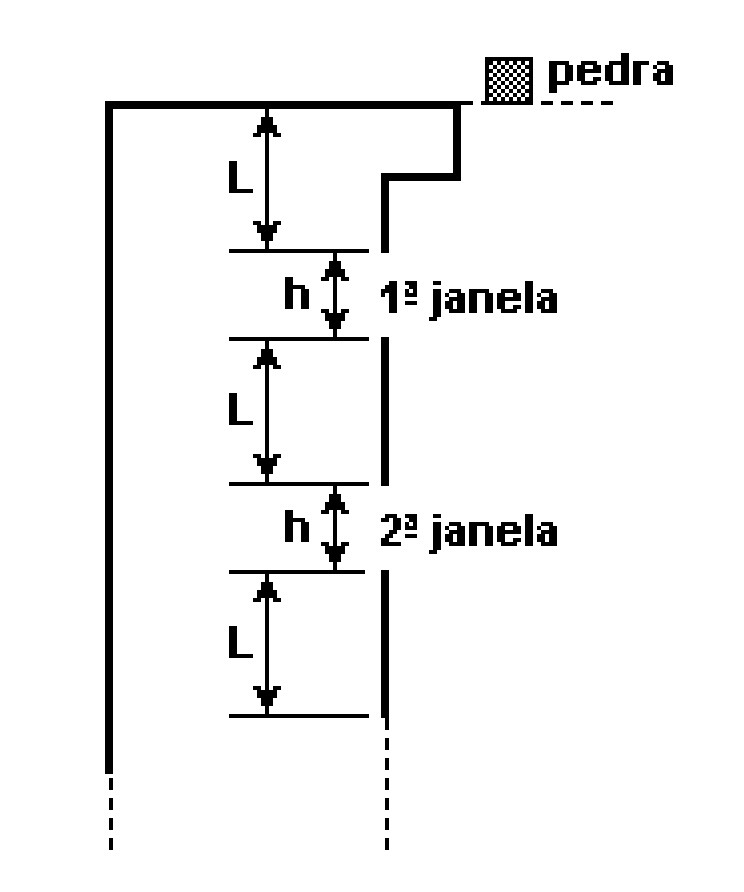
\includegraphics[width=0.25\linewidth]{imagensmecanica/funcaoposicaomuvITAexemplo.png}
\captionof{figure}{}
\label{fig_mec_funcaoposicaomuvITAjanelaexemplo}
} 

A figura mostra a disposição das janelas, com as pertinentes alturas $h$ e distâncias $L$ que se repetem igualmente para as demais janelas, até o térreo. Se a pedra percorre a altura $h$ da primeira janela em $t$ segundos, quanto tempo levará para percorrer, em segundos, a mesma altura $h$ da quarta janela? (Despreze a resistência do ar.)

\begin{enumerate}
  \item [(a)] 
  \left(
  \frac{\sqrt{L+h}-\sqrt{L}}
       {\sqrt{2L+2h}-\sqrt{2L+h}}
  \right)t$
  
  \item [(b)]
  \left(
  \frac{\sqrt{2L+2h}-\sqrt{2L+h}}
       {\sqrt{L+h}-\sqrt{L}}
  \right)t$
  
  \item [(c)]
  \left(
  \frac{\sqrt{4(L+h)}-\sqrt{3(L+h)+L}}
       {\sqrt{L+h}-\sqrt{L}}
  \right)t$
  
  \item [(d)]
  \left(
  \frac{\sqrt{4(L+h)}-\sqrt{3(L+h)+L}}
       {\sqrt{2L+2h}-\sqrt{2L+h}}
  \right)t$
  
  \item [(e)]
  \left(
  \frac{\sqrt{3(L+h)}-\sqrt{2(L+h)+L}}
       {\sqrt{L+h}-\sqrt{L}}
  \right)t$
\end{enumerate}


\resolucao



Considere um eixo vertical orientado para baixo com origem na posição em que a pedra é abandonada. Logo, a função horária da posição da pedra é

$$ s(t)=\cancelto{0}{s_0}+\cancelto{0}{v_0}t+\dfrac{1}{2}at^2 \implies s(t)=\dfrac{g}{2}t^2.$$

Sejam $s_{A}$ e $s_{B}$ as posições da pedra logo antes de adentrar na região da primeira janela e logo depois de tê-la percorrido. Sejam $t_A$ e $t_B$ os instantes de tempo respectivos de tais posições, de modo que, pelo enunciado, temos que $t_B - t_A = t.$ Assim, temos:

\begin{align}
    s_A &= L = \dfrac{g}{2}t_A^2 \implies t_A = \sqrt{\dfrac{2L}{g}}. \nonumber \\
    s_B &= L+h = \dfrac{g}{2}t_B^2 \implies t_B = \sqrt{\dfrac{2(L+h)}{g}}. \nonumber 
\end{align}

Subtraindo as duas equações acima e usando que $t_B - t_A = t,$ teremos

$$ t =  \sqrt{\dfrac{2(L+h)}{g}} - \sqrt{\dfrac{2L}{g}},$$

\noindent de onde tiramos, isolando o termo $\sqrt g,$ que

$$ \sqrt g = \dfrac{\sqrt{2(L+h)}-\sqrt {2L}}{t}.$$

Sejam $s_{C}$ e $s_{D}$ as posições da pedra logo antes de adentrar na região da quarta janela e logo depois de tê-la percorrido. Sejam $t_C$ e $t_D$ os instantes de tempo respectivos de tais posições. Queremos encontrar quanto vale $\Delta t =t_D - t_C,$ o intervalo de tempo entre tais posições. Assim, temos:

\begin{align}
    s_C &= 4L+3h = \dfrac{g}{2}t_C^2 \implies t_C = \sqrt{\dfrac{2(4L+3h)}{g}}. \nonumber \\
    s_D &= 4L+4h = \dfrac{g}{2}t_D^2 \implies t_D = \sqrt{\dfrac{2(4L+4h)}{g}}. \nonumber 
\end{align}

Subtraindo as duas equações acima, temos que o intervalo de tempo $\Delta t$ pedido é

$$ \Delta t = t_D - t_C =\sqrt{\dfrac{2(4L+4h)}{g}} - \sqrt{\dfrac{2(4L+3h)}{g}},$$

\noindent e, usando o valor da $\sqrt g$ obtido anteriormente, teremos

$$ \Delta t = \left( \dfrac{\sqrt{2(4L+4h)} -\sqrt{2(4L+3h)}}{\sqrt{2(L+h)} - \sqrt{2L}} \right) t,$$

\noindent dividindo o numerador e o denominador por $\sqrt 2$ teremos

$$ \Delta t = \left( \dfrac{\sqrt{4L+4h} -\sqrt{4L+3h}}{\sqrt{L+h} - \sqrt{L}} \right) t,$$

\noindent de modo que a resposta correta é a letra C.
  

\end{exemplo}

\vspace{0.3cm}





\begin{secnivel}[Equação de Torricelli]{I}{Equação de Torricelli}
 

  \eqLdois{dem}{mecanica_eq_torricelli}{v^2=v_0^2 + 2a \Delta s}
  
\end{secnivel}










\secgfe{De onde vem}

Tudo que você precisa saber, para estudar qualquer tipo de movimento, é saber exatamente aonde aquela partícula está em cada tempo -- saber sua \textbf{posição} -- e saber para onde ela está indo naquele instante de tempo -- \textbf{sua velocidade}. Dito isso, sabendo a \textit{função horária da posição} e a \textit{função horária da velocidade} você saberá tudo a respeito daquele movimento, qualquer que ele o seja. Logo, isso vale, naturalmente, para o Movimento Uniformemente Variado.

Assim, qualquer problema de Cinemática envolvendo um MUV poderá ser resolvido usando as duas equações anteriores, ou seja, as Equações \eqref{mecanica_eq_muvfuncaoposicao} e \eqref{mecanica_eq_muvfuncaovelocidade} são capazes de resolver absolutamente qualquer problema no contexto do MUV. Dito isso, a Equação \eqref{mecanica_eq_torricelli} é uma consequência daquelas duas últimas, isto é, ela é construída a partir das duas, com o intuito de resolver certos tipos de problemas com mais agilidade. 


\begin{figure}[h]
    \centering
    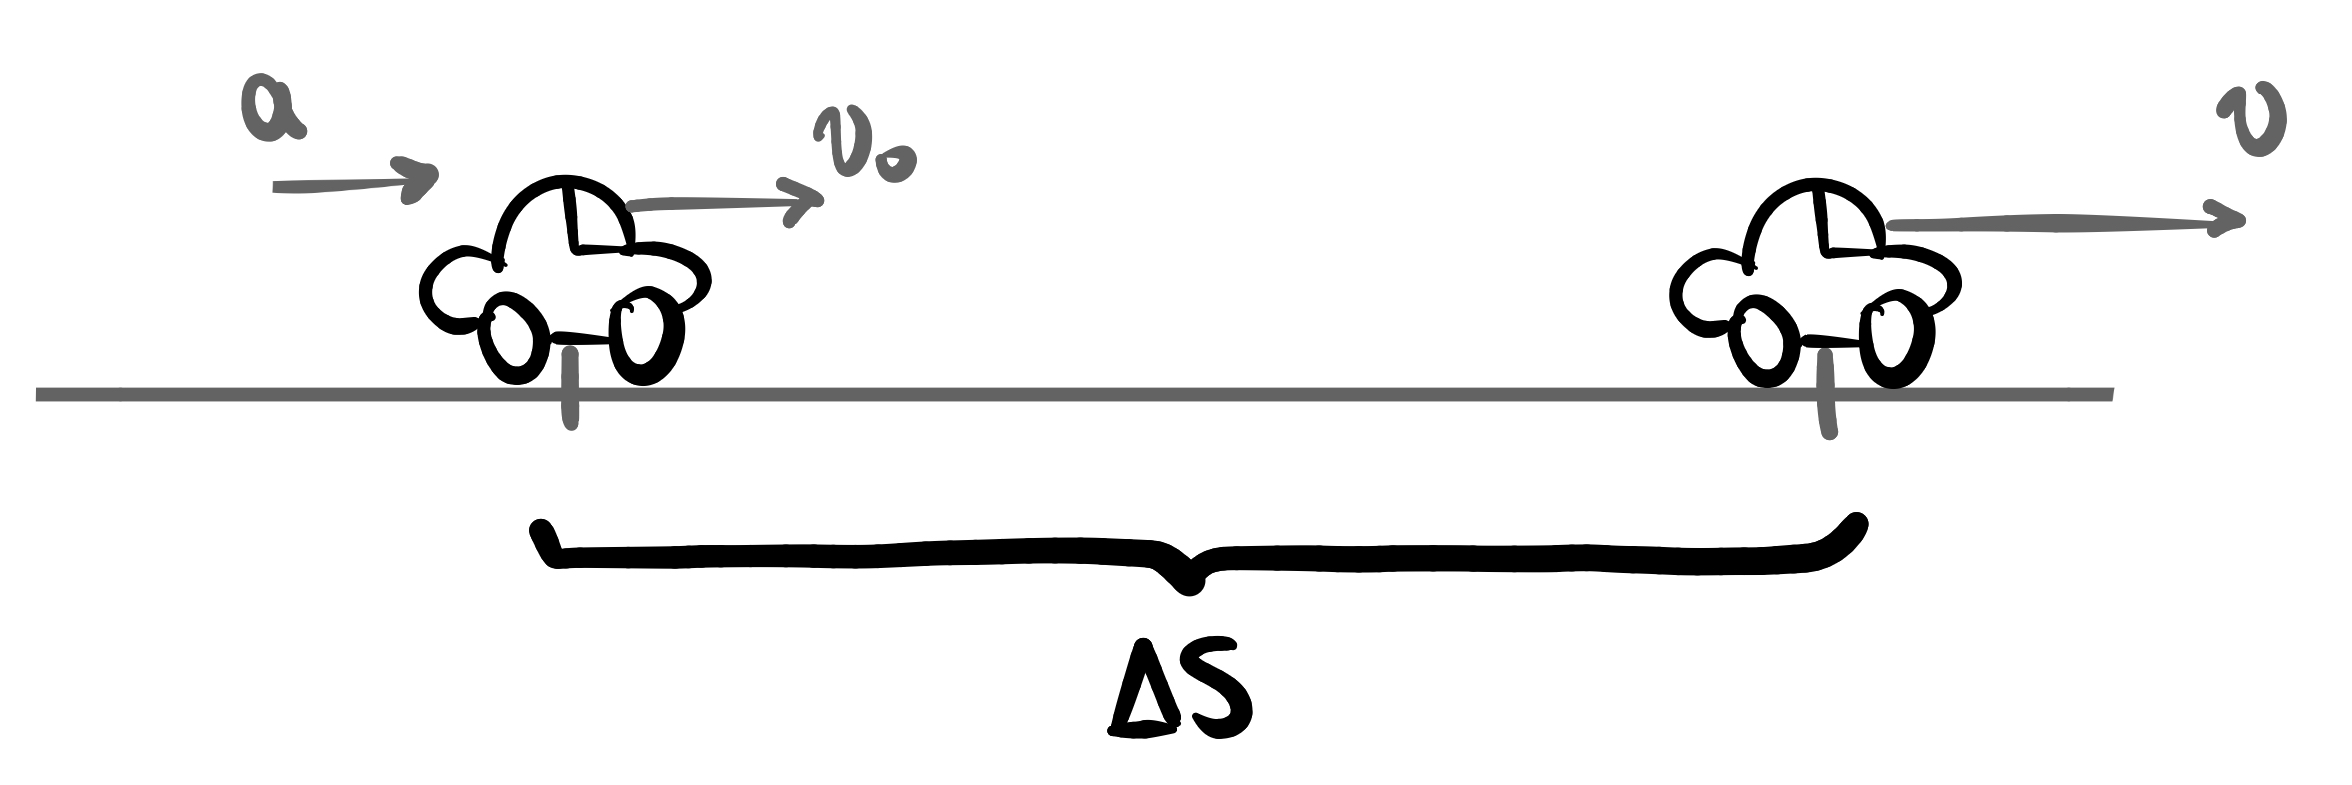
\includegraphics[scale=0.12]{imagensmecanica/torricelli02.jpeg}
    \caption{A construção da Equação de Torricelli.}
    \label{fig_mec_torricelli02}
\end{figure}

Tal equação envolve eliminarmos o tempo como variável para construir uma equação final que não dependa dele. Para tal, considere a Figura \ref{fig_mec_torricelli02}, que mostra um carro em Movimento Uniformemente Variado, com velocidade inicial $v_0$ e uma velocidade final, após um deslocamento $\Delta s$, igual a $v.$ Queremos relacionar essas três grandezas, sem envolver o tempo. Note que, por se tratar de um MUV, ele é governado pelas Equações \eqref{mecanica_eq_muvfuncaoposicao} e \eqref{mecanica_eq_muvfuncaovelocidade}. Podemos eliminar o tempo em uma delas e substituir na outra, a fim de alcançar o que pretendemos. Ou seja, nossos passos são:

\begin{itemize}
    \item [(i)] Usar a função horária da velocidade -- a Equação \eqref{mecanica_eq_muvfuncaovelocidade} -- para eliminar o tempo:

    $$ v = v_0 + at \implies v- v_0 = at \implies \boxed{t = \dfrac{v-v_0}{a} .}$$

     \item [(ii)] Substituímos tal resultado na função horária da posição para o MUV -- a Equação \eqref{mecanica_eq_muvfuncaoposicao} -- a fim de eliminar o tempo:

     \begin{align}
    \Delta s &= v_0t + \dfrac{1}{2}at^2 \nonumber \\
       &= v_0 \left( \dfrac{v-v_0}{a} \right) +\dfrac{1}{2}a \left( \dfrac{v-v_0}{a} \right)^2 \nonumber\\
       &= \dfrac{v_0v-v_0^2}{a} + \dfrac{\cancel{a}}{2} \left( \dfrac{v^2 -2vv_0 + v_0^2}{a^\cancel{2}} \right) \nonumber\\
       &= \dfrac{v^2-v_0^2}{2a}, \nonumber
     \end{align}
      \noindent de onde segue que $v^2 = v_0^2 +2a \Delta s$, como queríamos demonstrar.
\end{itemize}




\secgfe{Onde é usada}

Ela é usada em quaisquer problemas de Cinemática, envolvendo especificamente o Movimento Uniformemente Variado, nos quais não estamos interessados -- ou não temos informação -- a respeito do tempo. Note que, na Equação de Torricelli, o tempo não aparece em nenhum membro da equação. Em tais tipos de problemas, usar tal equação \textbf{não é obrigatório}, mas, em geral, \textbf{encurta e simplifica a resolução do problema}, como veremos no exemplo a seguir.

Considere o problema de se computar o deslocamento sofrido pelo carro da Figura \ref{fig_mec_torricelli} ao longo dos dois instantes registrados.

\begin{figure}[h]
    \centering
    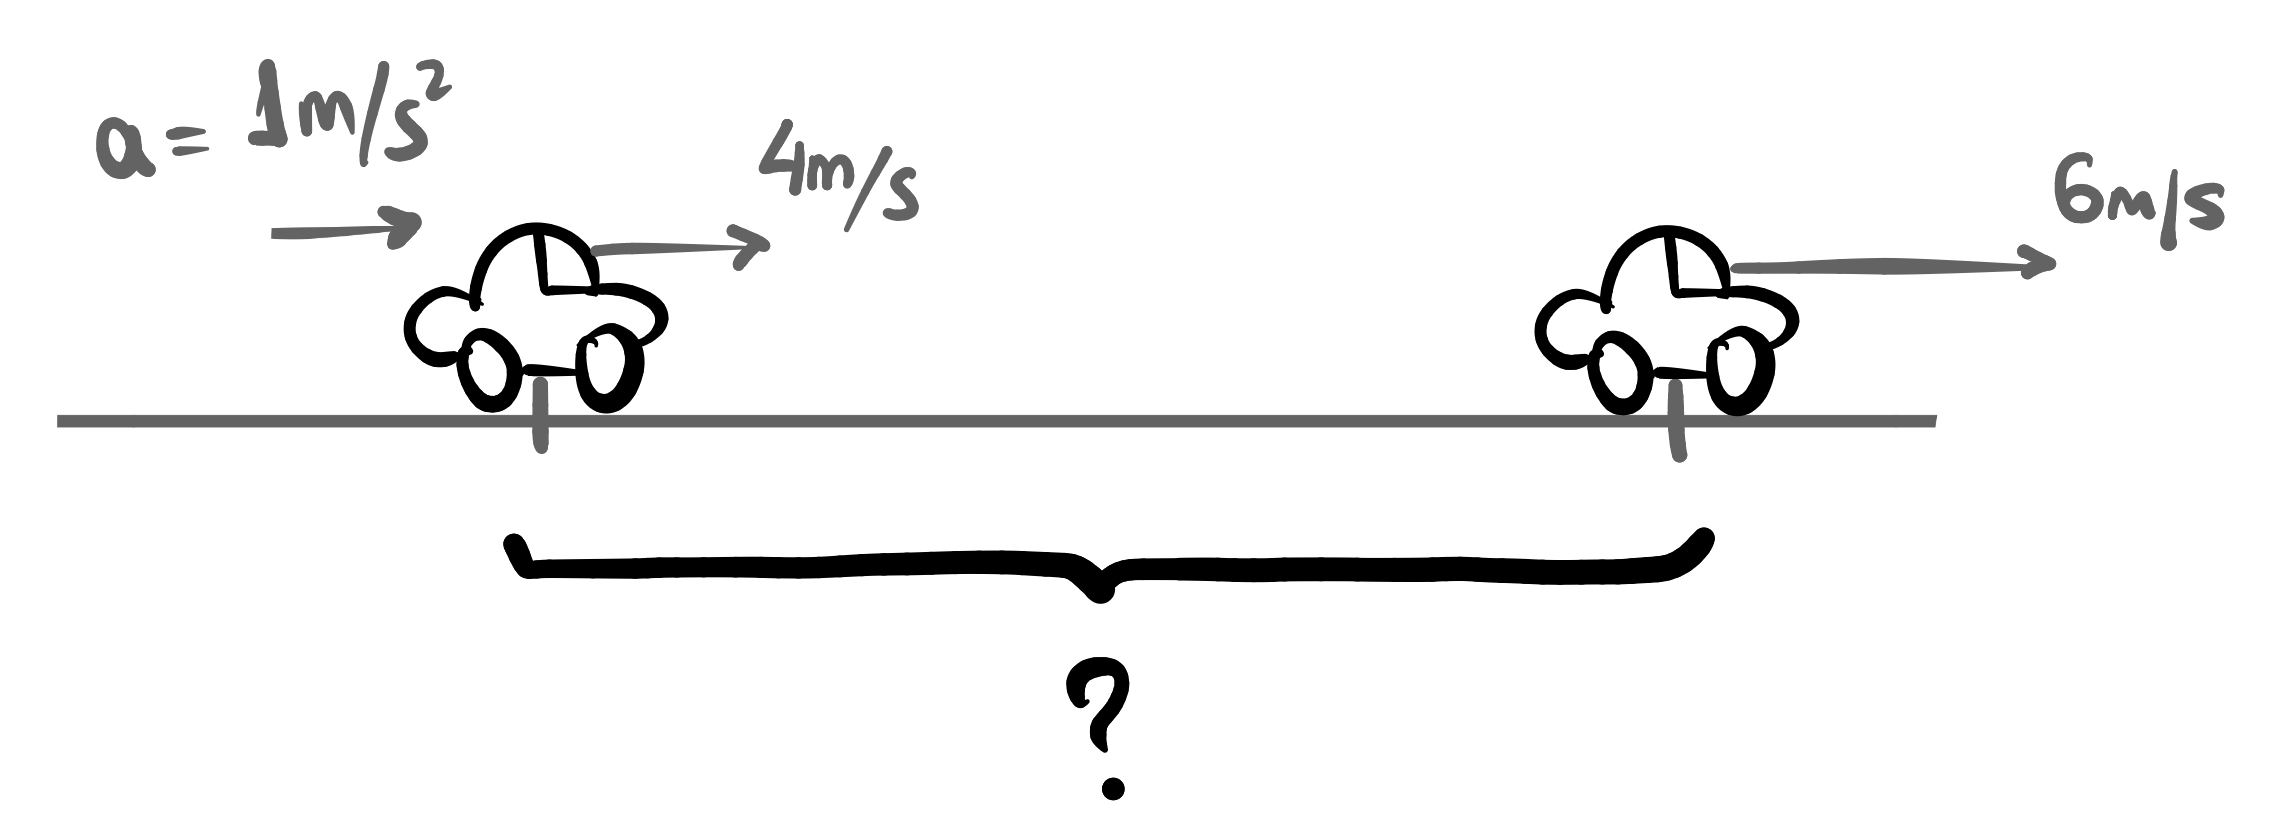
\includegraphics[scale=0.12]{imagensmecanica/torricelli01.jpeg}
    \caption{Construindo uma equação cinemática independente do tempo.}
    \label{fig_mec_torricelli}
\end{figure}

Perceba que não temos nenhuma informação a respeito do tempo que dura tal movimento -- e tampouco estamos interessados em tê-la: queremos saber apenas sobre o deslocamento. Contudo, caso não tivéssemos percebido isso, poderíamos prosseguir, em uma primeira abordagem, da seguinte maneira: como queremos computar o deslocamento, parece mais imediato usar a Equação \eqref{mecanica_eq_muvfuncaoposicao}, que fornece diretamente o valor do deslocamento $\Delta s$ por meio de

$$ \Delta s = v_0t + \dfrac{1}{2}at^2.$$

Contudo, olhando para tal equação, nós sabemos quanto vale a velocidade inicial $v_0$ e a aceleração $a$, porém não sabemos quanto tempo transcorreu desde o instante inicial até o final, no qual a velocidade atinge o valor de 6 m/s. Desse modo, para usar tal equação e resolver o problema, precisaríamos, antes, dar um passo intermediário e computar quanto tempo transcorreu entre aqueles dois instantes. O raciocínio, portanto, ocorreria em duas etapas, como se segue:

\begin{itemize}
    \item [(i)] Cálculo do tempo

    Usamos a Equação \eqref{mecanica_eq_muvfuncaovelocidade} para descobrir quanto tempo se passou entre as duas posições do carro, ou seja:

    $$ v= v
    _0+at \implies 6 = 4+1\cdot t \implies \boxed{t=2s.}$$

    \item [(ii)] Agora, munidos de tal resultado, podemos finalmente usar a Equação \eqref{mecanica_eq_muvfuncaoposicao} e computar o deslocamento que pretendíamos:

    $$ \Delta s = v_0t + \dfrac{1}{2}at^2 \implies \Delta s = 4 \cdot 2 + \dfrac{1}{2}\cdot 1 \cdot 2^2 \implies \boxed{ \Delta s = 10\text{m.}}$$
\end{itemize}

Uma segunda solução para tal problema -- e mais direta, como veremos -- seria o leitor perceber que o tempo não nos interessa, de modo que o passo inicial de computá-lo, como feito na solução anterior, acaba sendo desnecessário. 

Sendo assim, poderíamos usar direto a Equação de Torricelli que, como o leitor viu em sua demonstração, é construída justamente ao eliminar o tempo em uma equação e substituir na outra, ou seja, ela já contém, em seu pressuposto, a eliminação da etapa intermediária de se computar o tempo. Sendo assim, nossa resolução seria:

$$ v^2=v_0^2 + 2a \Delta s \implies 6^2 = 4^2+2 \cdot 1 \cdot \Delta s \implies \boxed{ \Delta s = 10\text{m}.}$$

Chegamos, naturalmente, na mesma resposta, porém realizando menos etapas. Note que, em tal solução, não sabemos quanto tempo durou o movimento -- mas nunca estivemos interessados em sabê-lo, desde o princípio. Por eliminar essa etapa intermediária do cálculo do tempo -- que é a premissa da Equação de Torricelli -- é que tal solução ficou mais curta e objetiva.





\secgfe{Erros comuns}

Os erros mais comuns quanto ao uso dessa equação são dois:

\begin{itemize}
    \item [(i)] Querer usá-la para outros movimentos que não sejam o Movimento Uniformemente Variado. Note que a Equação de Torricelli foi \textbf{construída} a partir das Equações \eqref{mecanica_eq_muvfuncaoposicao} e \eqref{mecanica_eq_muvfuncaovelocidade}, que são equações que \textbf{valem exclusivamente para um objeto que se move com aceleração constante}, ou seja, um objeto que esteja em um Movimento Uniformemente Variado. Logo, por conseguinte, a Equação de Torricelli também só valerá neste regime. 

    Se tentarmos aplicá-la para um corpo que descreve um Movimento Harmônico Simples (que será estudado posteriormente), um movimento com aceleração variável ou qualquer outro tipo de movimento que não seja o MUV, a equação, certamente, fornecerá resultados errados, por não valer em tais regimes.


    \item [(ii)] O sinal da aceleração.

    % Perceba que, ao fazermos a demonstração matemática da Equação \eqref{mecanica_eq_torricelli}, usamos como passo intermediário a equação $v=v_0+at,$ na qual a aceleração e as velocidades possuem o mesmo sinal. Ou seja, partimos da premissa de que o movimento era acelerado.

    % Se fizéssemos a demonstração para um movimento retardado, chegaríamos -- como o leitor pode fazer e verificar por si mesmo -- na equação

    % $$v^2 = v_0^2 - 2 a \Delta s. $$

    % Desse modo, a bem da verdade, teríamos duas equações de Torricelli: uma para o movimento acelerado, que é aquela descrita pela Equação \eqref{mecanica_eq_torricelli}, e uma para o movimento retardado, que é a equação acima. Contudo, essa segmentação parece mais complicar do que facilitar, e, como as duas equações são quase idênticas, a menos de uma troca de sinal, podemos optar por unificar as duas equações e dizer que há apenas uma: aquela descrita pela Equação \eqref{mecanica_eq_torricelli}. 

    % Para que isso seja verdade, basta convencionarmos que em tal equação a aceleração entra com sinal positivo em caso de movimento acelerado e sinal negativo em caso de movimento retardado. Com essa convenção, a equação se ajustará corretamente para cada caso. 

    % Assim, um erro comum é o aluno não se atentar a isso, e usar a aceleração como positiva na Equação \eqref{mecanica_eq_torricelli} para um movimento retardado, ou colocar o sinal negativo, sendo o movimento acelerado.

Perceba que, na demonstração da \eqref{mecanica_eq_torricelli}, usamos como passo intermediário
a Equação \eqref{mecanica_eq_muvfuncaovelocidade}, na qual a aceleração $a$ já carrega o seu sinal: ela é positiva
se aponta no mesmo sentido que o deslocamento, e negativa se aponta no sentido
contrário. Isso não é uma peculiaridade da demonstração --- é exatamente o mesmo
critério de sinal que usamos em toda a Cinemática.

Dito isso, há um erro bastante comum: o estudante identifica, por exemplo, que o
corpo está desacelerando e coloca o valor numérico da aceleração na equação sem sinal, obtendo
%
\begin{equation*}
    v^2 = v_0^2 + 2 \cdot 3 \cdot \Delta s,
\end{equation*}
%
\noindent para uma aceleração de $3$ m/s$^2$, no caso. Quando o correto seria inserir $a = -3\,\text{m/s}^2$, resultando em
%
\begin{equation*}
    v^2 = v_0^2 + 2\cdot(-3)\cdot\Delta s .
\end{equation*}

A regra é simples e a mesma que vale para todas as equações do MUV: defina
um referencial, atribua o sinal correto à aceleração dentro desse referencial, e
insira esse valor --- com sinal --- na Equação de Torricelli. A equação em si é sempre
a mesma; quem diferencia o movimento acelerado do retardado é o sinal de~$a$,
não uma fórmula diferente. De forma prática: movimentos acelerados carregarão aceleração positiva na Equação \eqref{mecanica_eq_torricelli}, enquanto movimentos retardados carregarão acelerações negativas.
    


    
\end{itemize}


\secgfe{Observações}

Cabe aqui uma breve observação sobre unidades de medida: a Equação de Torricelli envolve velocidades, aceleração e deslocamento. Se usarmos todas as grandezas em unidades de medida do SI, a respectiva grandeza calculada também irá ser fornecida em unidades do SI, ou seja:

\begin{itemize}
    \item Se usarmos $v_0$ em m/s, $a$ em m/s$^2$ e $\Delta s$ em m, então a equação irá nos fornecer o valor de $v$ em m/s.

    \item  Se usarmos $v_0$ em m/s, $v$ em m/s e $a$ em m/s$^2$, então a equação irá nos fornecer o valor de $\Delta s$ em m.

    \item Contudo, note que se usarmos $v_0$ em m/s, $v$ em km/h e $\Delta s$ em cm, então o autor há de lhe confessar que não faz a menor ideia de qual será a unidade de medida da aceleração que a equação irá fornecer. Ou seja, atente-se às unidades de medida que você coloca na equação para que o resultado final faça sentido.
    
    \end{itemize}



%Exemplo resolvido

\vspace{0.3cm}

\begin{exemplo}[Nível I]\label{exemplo_cinematicaescalar_torricelliex01}


Um carro, com velocidade inicial de 4 m/s, pisa no freio e imprime uma desaceleração constante de 1 m/s$^2$. Qual é a distância total percorrida por este veículo até parar?


\resolucao


A Figura \ref{fig_mec_torricelli03} ilustra a situação do problema. Note que trata-se de um problema em que não temos informação alguma a respeito do tempo, e tampouco pede-se para computar o tempo. Desse modo, usar a Equação \eqref{mecanica_eq_torricelli} parece ser um bom caminho. Assim, a solução é a que se segue:

$$ v^2=v_0^2 + 2a \Delta s \implies 0^2 = 4^2 +2 \cdot (-1) \cdot \Delta s \implies \boxed{ \Delta s = 8\text{m}.} $$

{
\centering
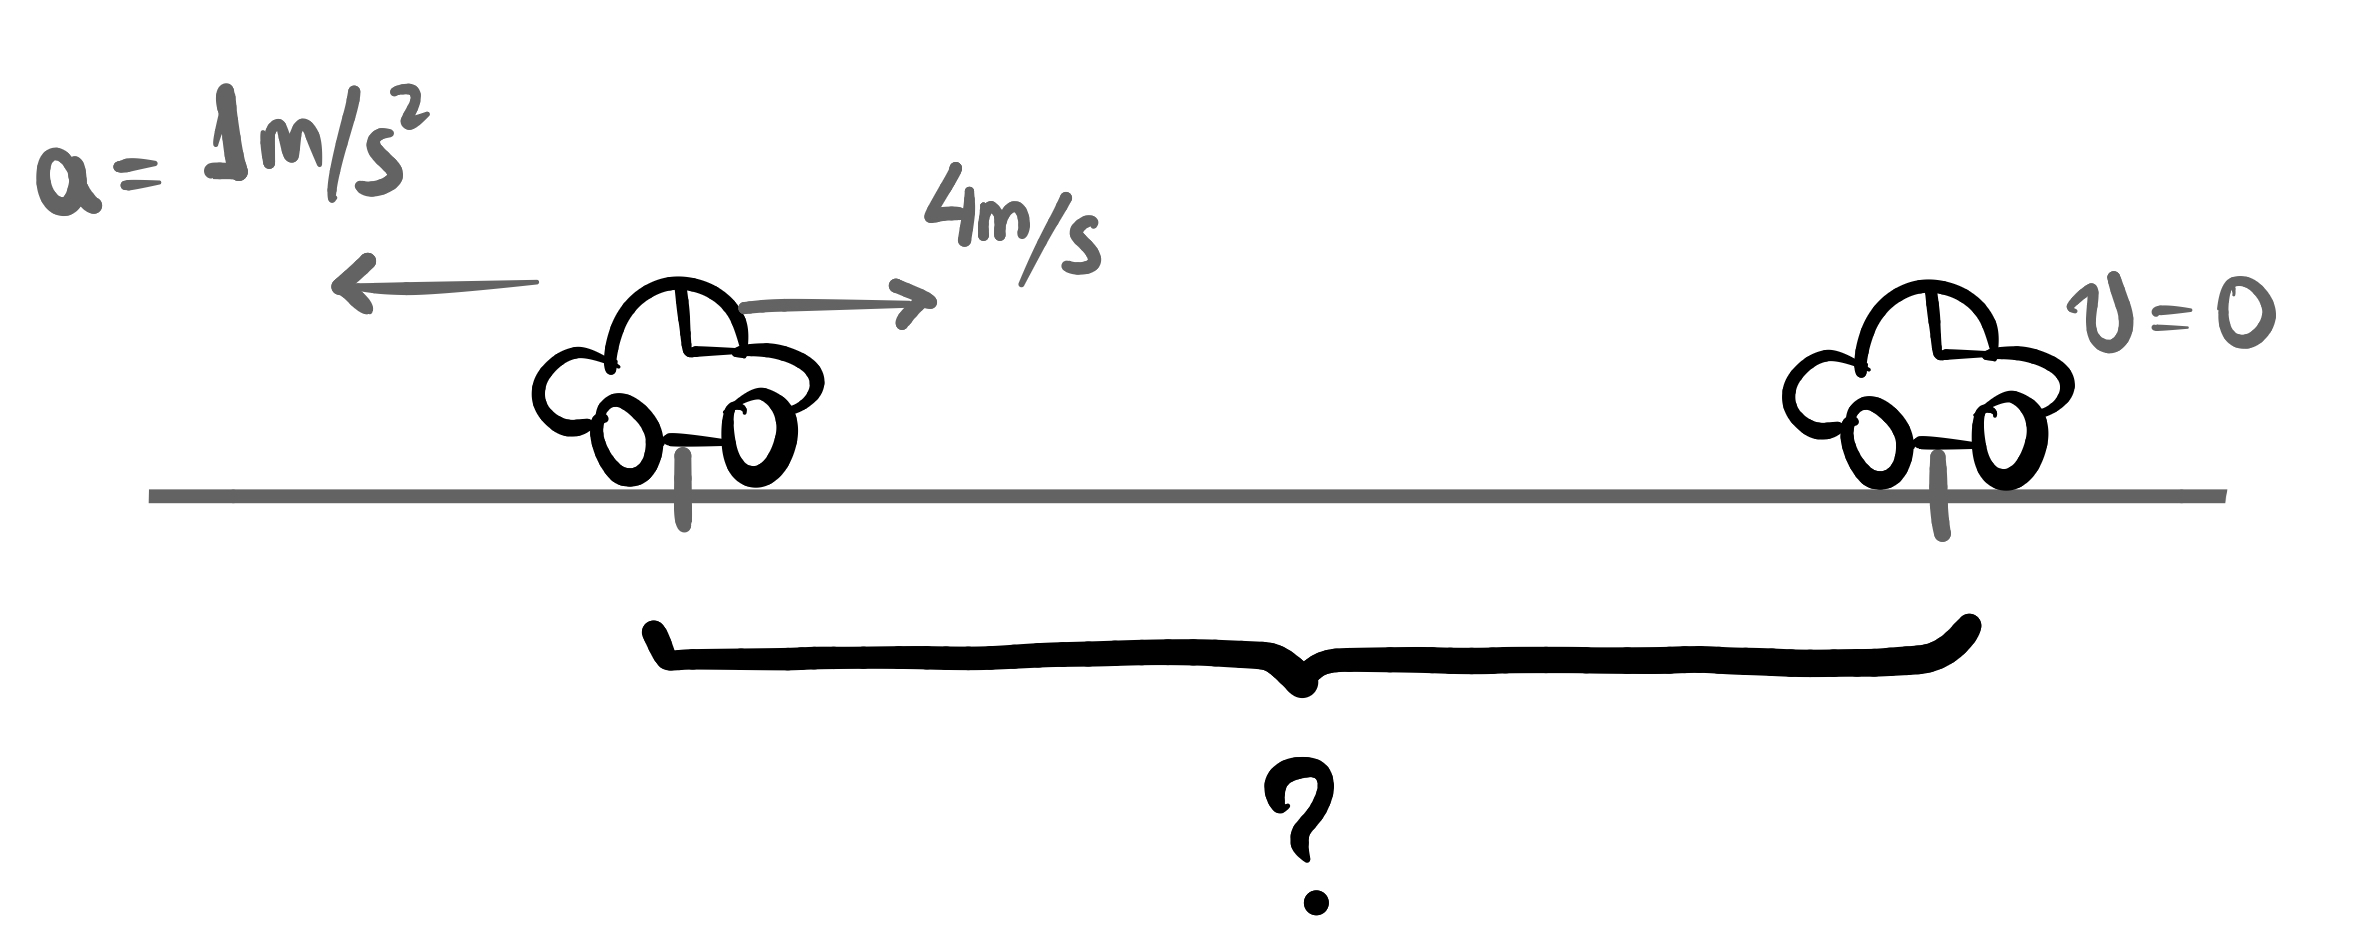
\includegraphics[width=0.5\linewidth]{imagensmecanica/torricelli03.jpeg}
\captionof{figure}{Carro freando com desaceleração constante.}
\label{fig_mec_torricelli03}
} 
\vspace{0.3cm}

Note que usamos a velocidade final $v$ como sendo $0$, uma vez que no instante final o carro estará parado. Além disso, como o movimento é retardado, a aceleração entra com sinal negativo na Equação de Torricelli.

\end{exemplo}

\vspace{0.3cm}







\begin{exemplo}[Nível II]\label{exemplo_cinematicaescalar_torricelliex02}


Dois corpos $A$ e $B$ movem-se ao longo da mesma reta. O corpo $A$ parte do repouso com aceleração constante $a$, enquanto o corpo $B$ parte do repouso, no mesmo instante e mesma posição de $A$, com aceleração constante $2a$. Quando $A$ atinge velocidade $v$ ele alcança uma certa posição. Encontre a velocidade de $B$ quando ele passar por essa mesma posição.


\resolucao


Para chegar na velocidade $v$, saindo do repouso, o corpo $A$ percorre uma distância $\Delta x_A,$ que pode ser obtida pela Equação \eqref{mecanica_eq_torricelli}:

$$ v^2 = \cancelto{0}{v_0^2}+2a \Delta x_A \implies \Delta x_A = \dfrac{v^2}{2a}.$$

Já o corpo $B$, partindo do mesmo ponto que $A,$ passará pela mesma posição que ele quando percorrer a mesma distância $\Delta x_A. $ Logo, sua velocidade $v_B$ nessa posição também pode ser obtida pela Equação \eqref{mecanica_eq_torricelli}:

$$ v_B^2 = \cancelto{0}{v_0^2}+2(2a) \Delta x_A \implies v_B^2 = 4a \dfrac{v^2}{2a} \implies \boxed{v_B = v\sqrt{2}.}$$


\end{exemplo}

\vspace{0.3cm}





% \begin{exemplo}[Nível III]\label{exemplo_cinematicaescalar_torricelliex03}



% Um corpo move-se em linha reta com velocidade inicial $v_0$ e deve ser freado até parar. Você dispõe de duas desacelerações constantes possíveis, de módulos $a_1$ e $a_2$ ($a_1\neq a_2$, ambas positivas). O procedimento de frenagem será o seguinte: primeiro aplica-se a desaceleração $a_1$ até a velocidade cair a $v_1$; em seguida aplica-se $a_2$ até o repouso. Você pode escolher livremente o valor de $v_1$ (isto é, o instante de troca).

% Determine o valor de $v_1$ que minimiza a distância total de frenagem e calcule essa distância mínima.


% \resolucao


% Usaremos a Equação \eqref{mecanica_eq_torricelli} nos dois trechos. Para o primeiro deles, temos:


% \medskip
% \textbf{Trecho 1:} de $v_0$ até $v_1$ com aceleração $-a_1$.
% Pela equação de Torricelli,
% \[
% v_1^2=v_0^2+2(-a_1)s_1
% \quad\implies\quad
% s_1=\frac{v_0^2-v_1^2}{2a_1}.
% \]

% \medskip
% \textbf{Trecho 2:} de $v_1$ até $0$ com aceleração $-a_2$.
% \[
% 0=v_1^2+2(-a_2)s_2
% \quad\implies\quad
% s_2=\frac{v_1^2}{2a_2}.
% \]

% \medskip

% A distância total percorrida até parar completamnete é $s=s_1+s_2$. Logo,
% \[
% s(v_1)= s_1+s_2 =\frac{v_0^2-v_1^2}{2a_1}+\frac{v_1^2}{2a_2}
% =\frac{v_0^2}{2a_1}+v_1^2\left(\frac{1}{2a_2}-\frac{1}{2a_1}\right).
% \]

% Perceba que todos os termos -- exceto $v_1$ -- são constantes e pré-determinados. Nossa função soma um termo que tem um coeficiente multiplicando $v_1^2$. Sendo $v_1^2$ sempre positivo, vamos analisar o sinal do coeficiente que o acompanha. Para tal, defina
% \[
% C=\left(\frac{1}{2a_2}-\frac{1}{2a_1}\right)=\frac{a_1-a_2}{2a_1a_2}.
% \]

% \medskip
% \textbf{Caso 1:} $a_2>a_1$ $\implies C<0$. Nesta caso $s$ diminui quando $v_1^2$ aumenta, já que o termo que contém $v_1^2$ fica sendo subtraído. Logo, o mínimo ocorre para o maior valor possível de $v_1,$ isto é, em $v_1=v_0$:
% \[
% s_{\min}=\frac{v_0^2-v_0^2}{2a_1}+\frac{v_0^2}{2a_2}=\frac{v_0^2}{2a_2}.
% \]

% \medskip
% \textbf{Caso 2:} $a_2<a_1$ $\Rightarrow C>0$. Neste caso $s$ aumenta quando $v_1^2$ aumenta, já que o termo que contém $v_1^2$ está sendo somado. Logo, o mínimo ocorre para o menor valor possível de $v_1$, isto é, em $v_1=0$:
% \[
% s_{\min}=\frac{v_0^2}{2a_1}.
% \]

% Note que, em um primeiro contato, parece um problema difícil, mas na verdade ele é bem fácil: use o maior valor de aceleração disponível e freie com ela durante todo o movimento -- essa é a forma de ter a frenagem mais eficiente e parar o carro na menor distância possível. Razoável, não?


% \end{exemplo}

\begin{exemplo}[Nível III]\label{exemplo_cinematicaescalar_torricelliex03}

Um corpo parte do repouso, acelera uniformemente com aceleração $a_1$ até atingir
velocidade $v_0$, e em seguida desacelera uniformemente com aceleração $a_2$ até
parar. Um segundo corpo parte simultaneamente do mesmo ponto com velocidade
constante $v_c$ e chega ao mesmo destino no mesmo instante. Determine $v_c$ e mostre
que o resultado independe de $a_1$ e $a_2$.

\resolucao

Calculemos o tempo e a distância de cada fase separadamente. Na \textit{fase de
aceleração}, o corpo parte do repouso e atinge $v_0$:

$$ t_1 = \frac{v_0}{a_1}, \qquad d_1 = \frac{v_0^2}{2a_1}. $$

Na \textit{fase de desaceleração}, o corpo parte de $v_0$ e para:

$$ t_2 = \frac{v_0}{a_2}, \qquad d_2 = \frac{v_0^2}{2a_2}. $$

Nos dois casos as distâncias percorridas foram obtidas pela Equação de Torricelli, e o tempo de percurso foi obtido pela Função Horária da Velocidade do MUV. O tempo total e a distância total são, portanto,

$$ T = t_1 + t_2 = v_0\!\left(\frac{1}{a_1}+\frac{1}{a_2}\right)
     = \frac{v_0(a_1+a_2)}{a_1 a_2}, $$

$$ D = d_1 + d_2 = \frac{v_0^2}{2}\!\left(\frac{1}{a_1}+\frac{1}{a_2}\right)
     = \frac{v_0^2(a_1+a_2)}{2\,a_1 a_2}. $$

Note que $D = v_0 T/2$. Logo, a velocidade constante equivalente é

$$ \boxed{v_c = \frac{D}{T} = \frac{v_0}{2}.} $$

O fator $(a_1+a_2)/(a_1 a_2)$ aparece tanto em $D$ quanto em $T$ e se cancela
inteiramente: $v_c$ não depende das acelerações.

Não importa se o corpo acelera devagar e freia bruscamente, ou o contrário --- sua
velocidade média é sempre exatamente metade da velocidade máxima alcançada por ele. Um corpo em movimento
uniforme a $v_0/2$ cobre a mesma distância no mesmo tempo, sempre.

\end{exemplo}
\vspace{0.3cm}




\begin{secnivel}[Velocidade Média no MUV]{II}{Velocidade Média no MUV}
 

  \eqLdois{dem}{mecanica_eq_muvvelocidademedia}{v_m = \dfrac{v_1+v_2}{2}}
  
\end{secnivel}








\secgfe{De onde vem}

Essa equação pode ser obtida de um modo bastante semelhante à construção feita para demonstrar a Equação \eqref{mecanica_eq_muvfuncaoposicao}, fazendo, para tanto, apenas uma pequena consideração.

Para entender tal consideração, observe a imagem da Figura \ref{fig_mec_trapezio01}, que mostra um trapézio, de bases $b$ e $B$ e altura $h.$ Pegando o ponto médio $M$ do quarto lado de tal trapézio, iremos construir, como mostra a segunda parte da figura, dois triângulos retângulos congruentes -- eles terão os três ângulos iguais, o que os faria semelhantes, porém suas hipotenusas possuem o mesmo tamanho, de modo que a razão de semelhança é 1 e, portanto, eles são congruentes. Uma semelhança de triângulos nos leva à conclusão de que a distância do ponto $M$ até o lado de tamanho $h$ é igual à média aritmética das bases do trapézio -- tal segmento é conhecido como base média do trapézio, e está destacado na segunda imagem da Figura \ref{fig_mec_trapezio01}.


\begin{figure}[h]
    \centering
    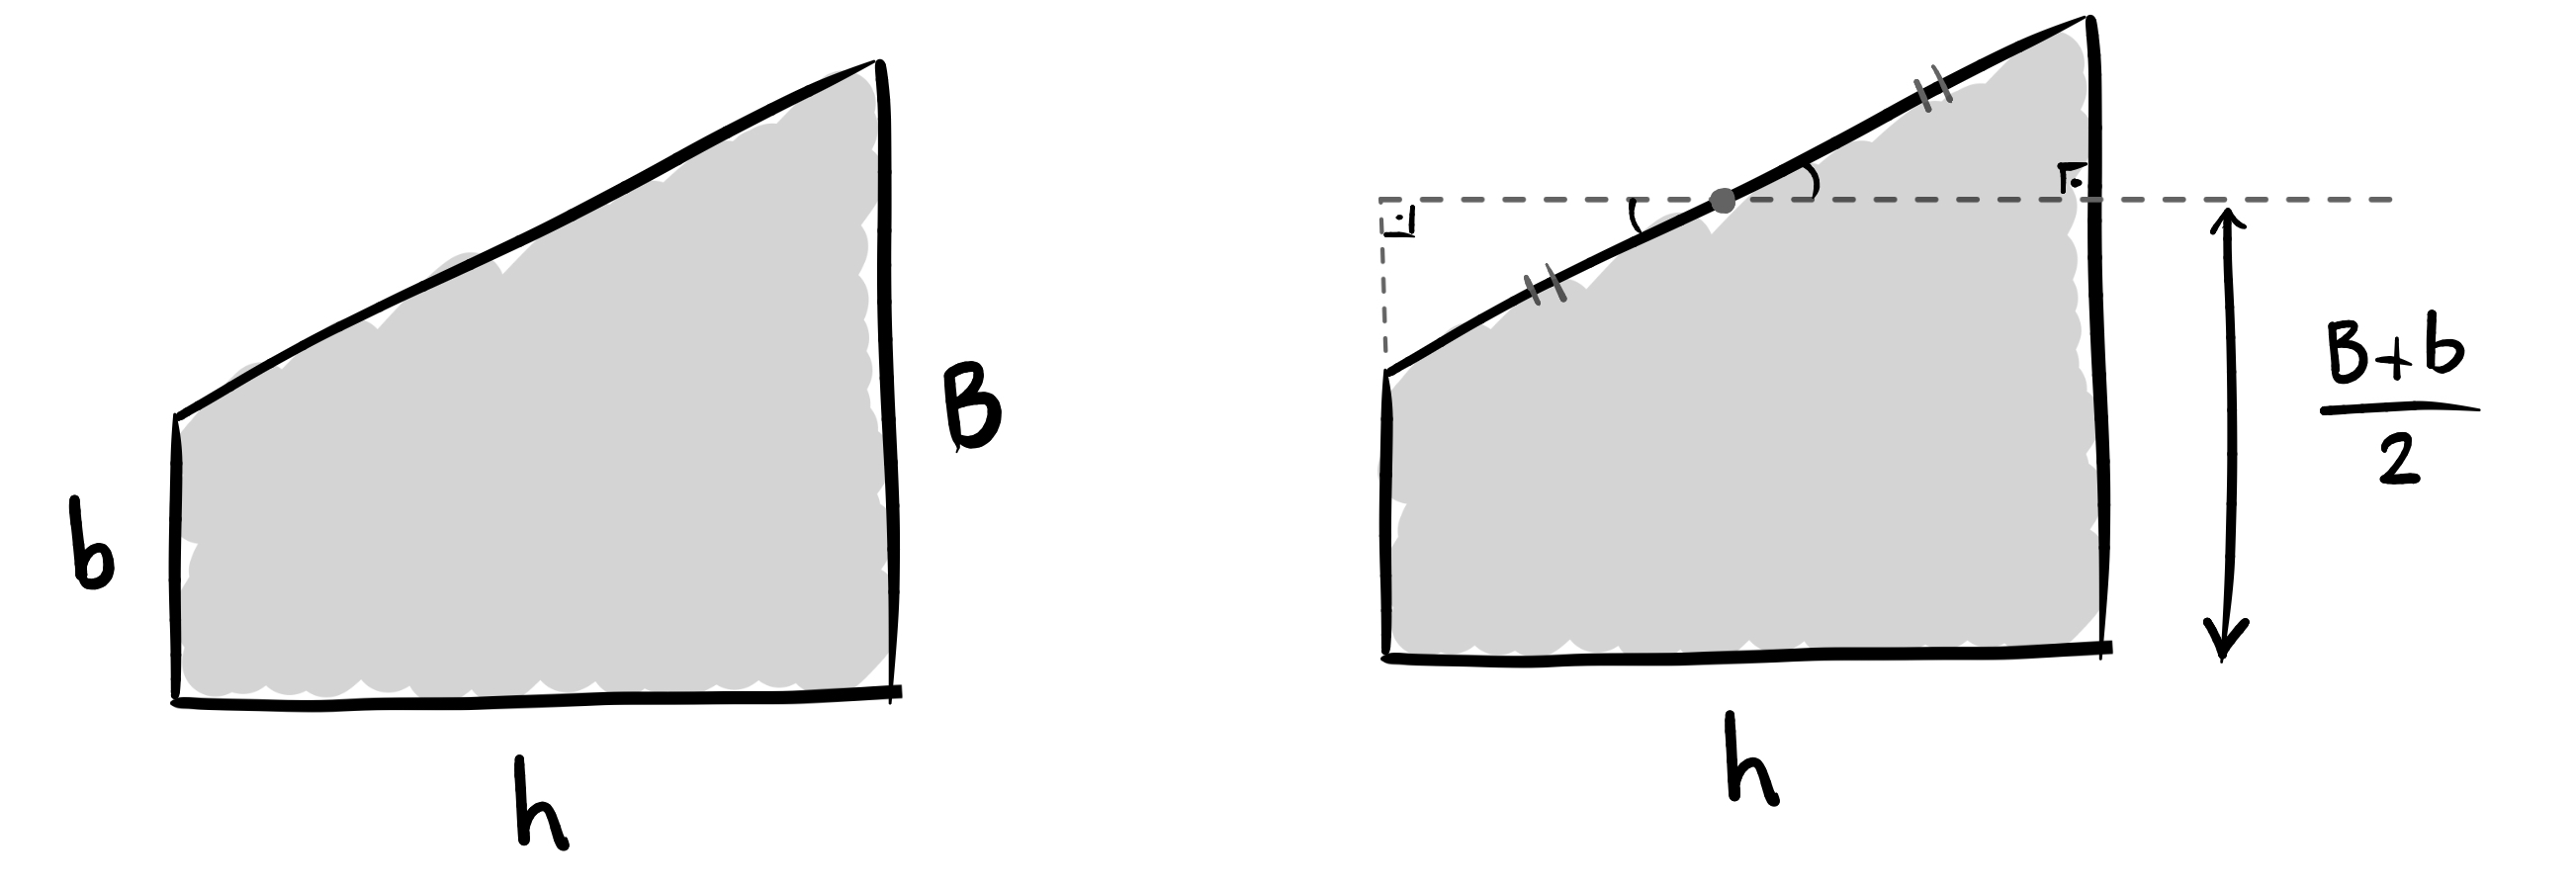
\includegraphics[scale=0.12]{imagensmecanica/muvtrapezio01.jpeg}
    \caption{A base média de um trapézio.}
    \label{fig_mec_trapezio01}
\end{figure}

Note agora que, devido às áreas dos dois triângulos retângulos serem iguais, poderíamos deslocar a área do triângulo do canto superior direito para o triângulo do canto inferior esquerdo. Isso modificaria a nossa figura geométrica sem alterar sua área -- tal processo é o que aparece na Figura \ref{fig_mec_trapezio02}.

Essa construção nos mostra que a área do trapézio de bases $b$, $B$ e altura $h$ é exatamente igual à área do retângulo de altura $\sfrac{(B+b)}{2}$ e altura $h$. Tal retângulo é o que aparece na imagem da direita da Figura \ref{fig_mec_trapezio02}. Ou seja, matematicamente:

$$ \dfrac{(B+b)\cdot h }{2} = \dfrac{(B+b)}{2}\cdot h,$$


\noindent em que o lado esquerdo é a forma tradicional de computar a área de um trapézio e o lado direito é o cálculo tradicional da área de um retângulo, isto é, bases vezes altura.



\begin{figure}[h]
    \centering
    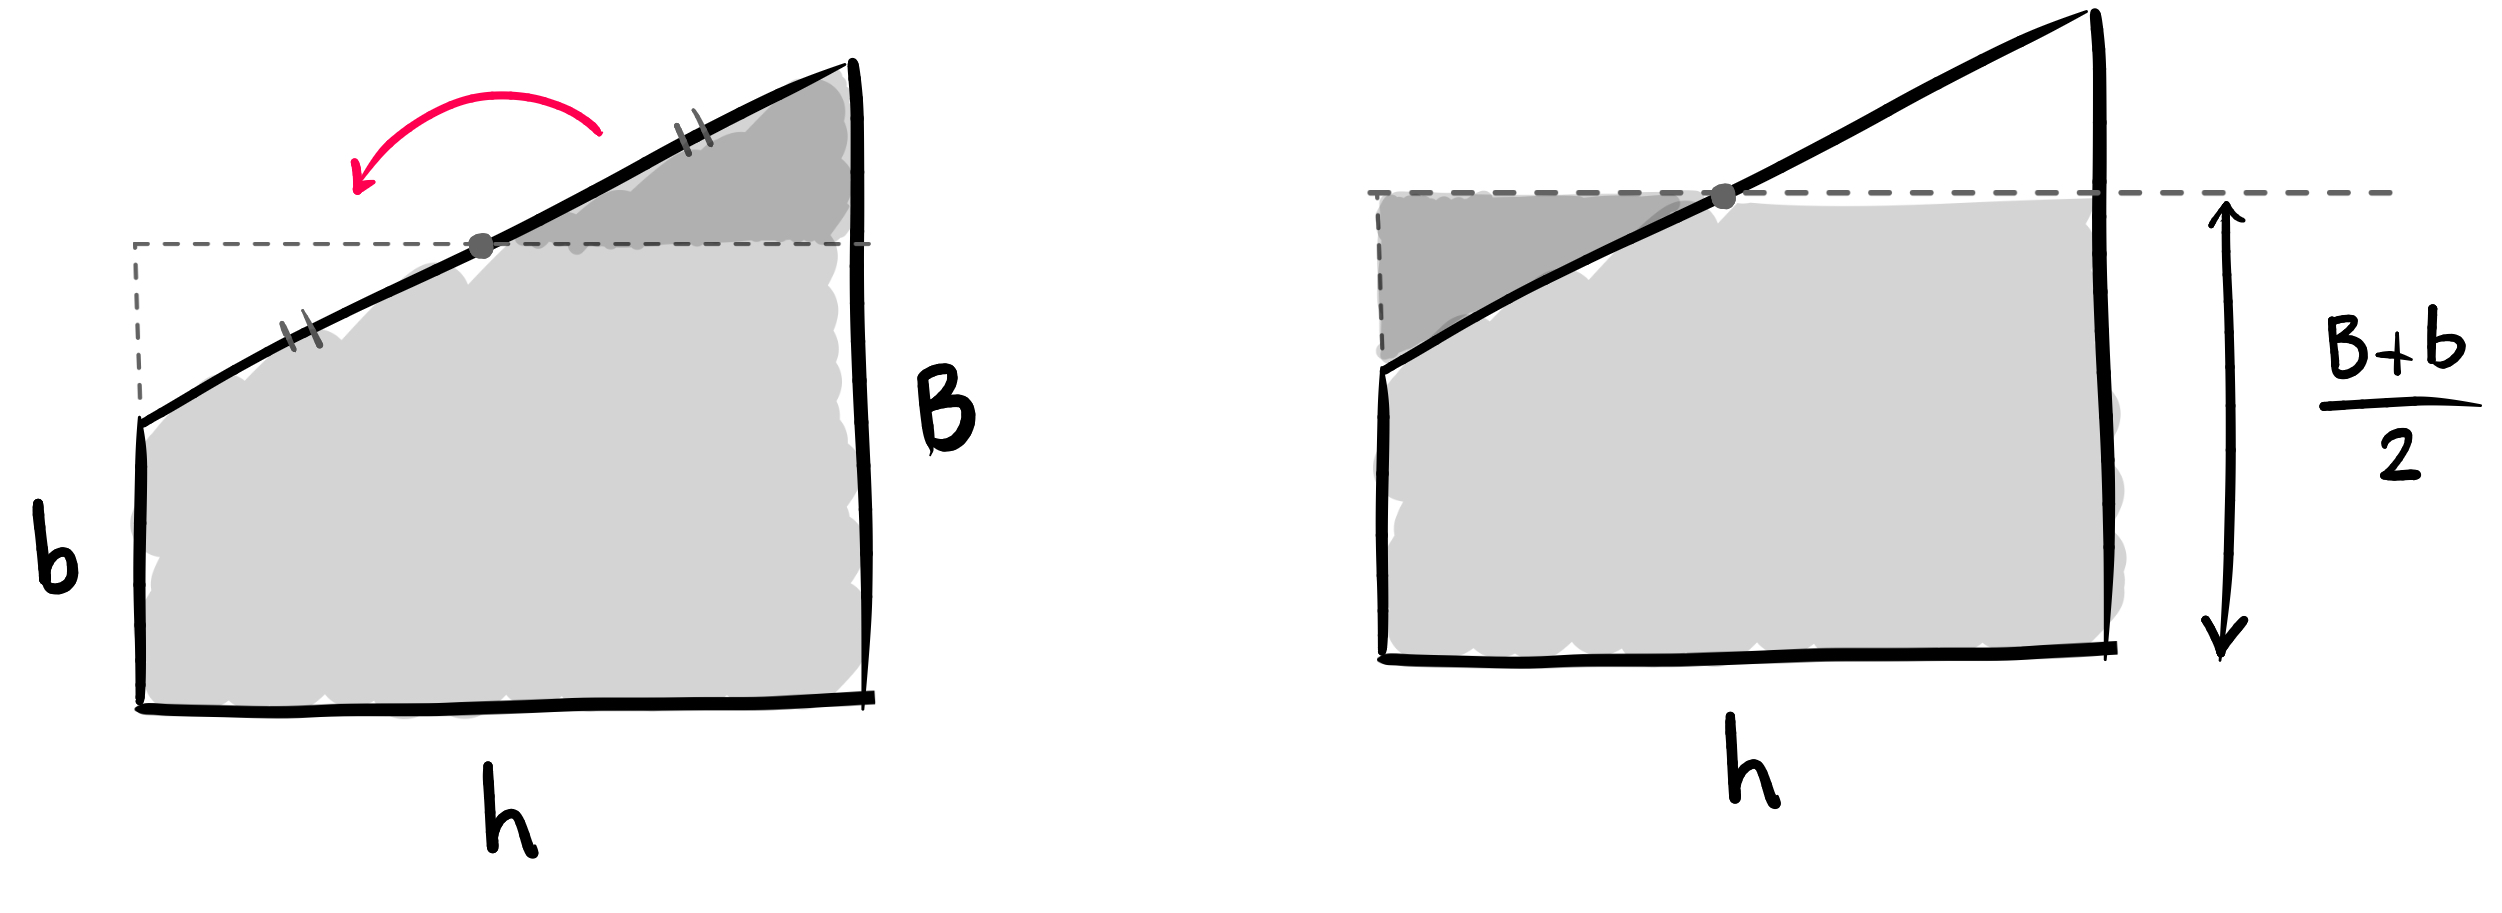
\includegraphics[scale=0.12]{imagensmecanica/muvtrapezio02.jpeg}
    \caption{Modificando a figura sem alterar sua área.}
    \label{fig_mec_trapezio02}
\end{figure}


Dito isso, voltemos agora à construção da Equação \eqref{mecanica_eq_muvfuncaoposicao}, a qual partiu do cálculo da área abaixo do gráfico de velocidade por tempo, destacado na Figura \ref{fig_mec_graficovxt}. Ora, a Figura \ref{fig_mec_trapezio03} evidencia que há duas formas de se calcular tal área: calculando diretamente à área do trapézio, como foi feito na construção da Equação \eqref{mecanica_eq_muvfuncaoposicao}; ou calculando a área do retângulo de mesma altura, porém cuja base é igual à média aritmética das bases do trapézio -- sua base média. 

Neste caso, vemos com clareza que as bases do nosso trapézio são as velocidades inicial $v_0$ e final $v$ do corpo em movimento, de modo que sua base média é 

$$ v'=\dfrac{v_0+v}{2}.$$



\begin{figure}[h]
    \centering
    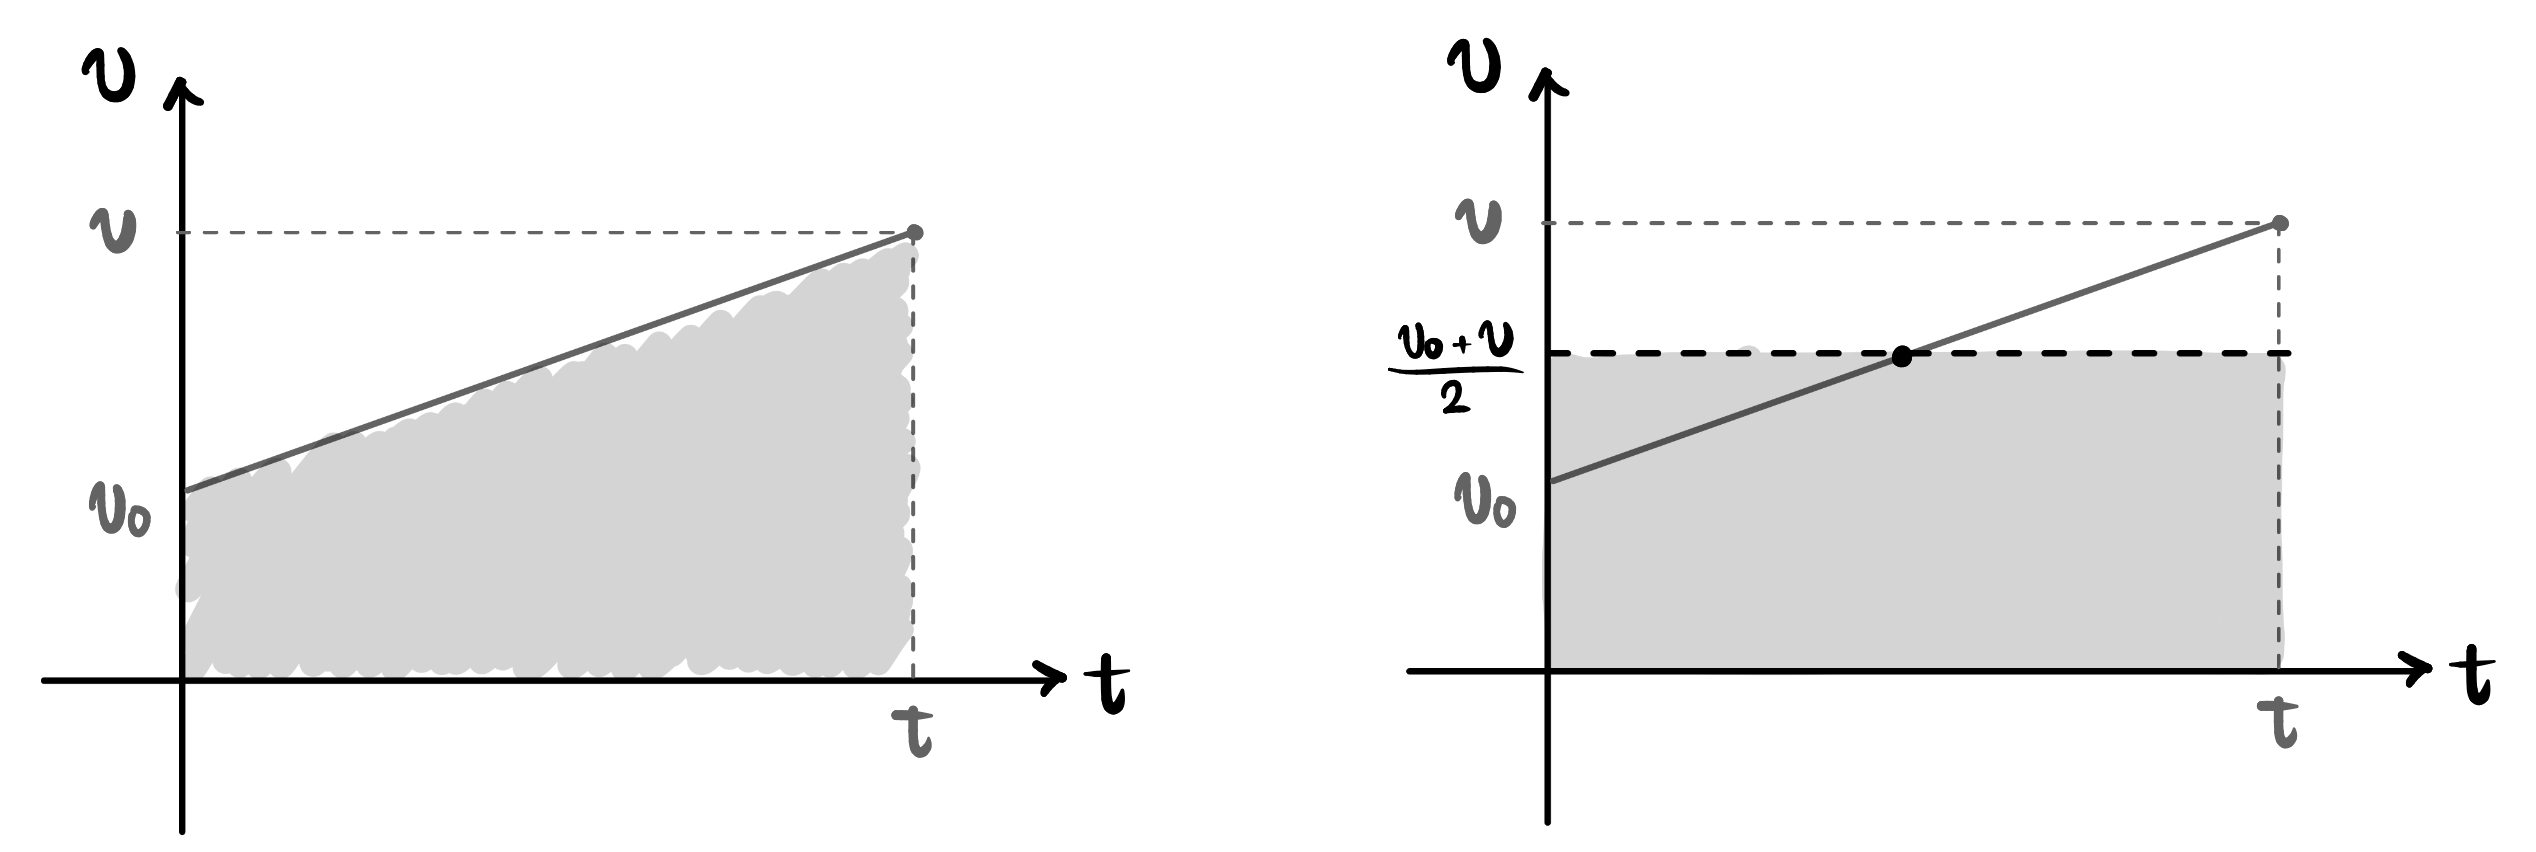
\includegraphics[scale=0.12]{imagensmecanica/muvtrapezio03.jpeg}
    \caption{A equivalência da área do trapézio e do retângulo cuja base é igual à sua base média.}
    \label{fig_mec_trapezio03}
\end{figure}

Ora, se a área abaixo do gráfico é igual ao deslocamento $\Delta s$, podemos computar tal área por meio do retângulo da direita da Figura \ref{fig_mec_trapezio03}:

$$ \Delta s = b \cdot h= \dfrac{(v_0+v)}{2} \cdot t,$$
e, pela definição de velocidade média feita na Equação \eqref{mecanica_eq_velocidademedia}, temos que
$$ \Delta s = v_m \cdot t,$$

\noindent e, igualando as duas últimas equações, chegamos finalmente em

$$ v_m =  \dfrac{(v_0+v)}{2}.$$

Isso quer dizer que, apesar das observações feitas quando definimos a velocidade média -- sendo a principal delas o fato de que calcular a \textbf{velocidade média não é o mesmo que calcular a média das velocidades}, essas duas coisas, curiosamente, coincidem no MUV. É isso que a Equação \eqref{mecanica_eq_muvvelocidademedia} diz: a velocidade média -- exclusivamente no MUV -- em um certo intervalo de tempo é igual à média das velocidades do corpo nos extremos de tal intervalo.

Para deixar absolutamente claro o que fizemos aqui: não estamos dizendo que velocidade média e média aritmética das velocidades são a mesma coisa. Não estamos mudando a definição do conceito de velocidade média -- a velocidade média continua sendo definida pela Equação \eqref{mecanica_eq_velocidademedia}. O que fizemos aqui foi perceber que, exclusivamente para o MUV, a velocidade média, definida exatamente como está na Equação \eqref{mecanica_eq_velocidademedia}, coincide com a média das velocidades.

\secgfe{Onde é usada}

Em problemas de MUV nos quais sabemos a velocidade inicial e final e se deseja calcular o deslocamento ao longo de tal intervalo de tempo, ou então o tempo para que um certo deslocamento ocorra.

É importante o leitor notar que essa equação não introduz nenhuma informação nova na nossa teoria -- ou seja, a princípio, ela é como a Equação de Torricelli: é desnecessária. Não é preciso sabê-la para resolver nenhum problema de MUV, mas, em alguns casos, ela pode ser um bom atalho e encurtar os cálculos, como veremos.


\secgfe{Erros comuns}

Aqui é preciso tomar cuidado, novamente, para não confundir deslocamento com distância. É tentador o leitor pensar que ele pode, agora, simplesmente aplicar a clássica equação $d=vt$ para o MUV, bastando para isso usar $v$ como sendo a média das velocidades. 

Isso está quase correto. Para perceber algumas nuances, voltemos ao contexto do problema descrito na Figura \ref{fig_mec_muvlancamentovertical}. Para os três primeiros segundos de movimento -- a subida -- poderíamos obter a velocidade média da partícula pela média das velocidades, que seria:

$$ v_m=\dfrac{v_0+v}{2}=\dfrac{30+0}{2}=15 \text{m/s}.$$

Assim, a distância percorrida nos três primeiros segundos seria simplesmente

$$d=v_mt=15\cdot 3 = 45 \text{m},$$

\noindent que é exatamente o valor que lá obtivemos, porém aqui de modo bem simples.

Se quiséssemos computar a distância percorrida ao longo dos 6 segundos de movimento poderíamos tentar algo parecido. Primeiro, façamos a velocidade média ao longo dos 6 segundos, que seria a média das velocidades inicial e final ao longo deste intervalo, ou seja:

$$  v_m=\dfrac{v_0+v}{2}=\dfrac{30+(-30)}{2}= 0 \text{m/s}.$$

Parece que ficou estranho. Se optarmos por prosseguir, computaríamos que a distância percorrida neste trecho é

$$ d=v_m t = 0 \cdot 6 = 0 \text{m},$$

\noindent o que está claramente errado.

O erro foi em trocar distância por deslocamento. A equação correta, que vem da definição de velocidade média feita na Equação \eqref{mecanica_eq_velocidademedia}, é que 

$$ \Delta s = v_m \cdot t,$$

\noindent ou seja, o produto da velocidade média pelo tempo fornece o deslocamento, e não a distância. Cabe novamente destacar que, em movimentos cujo sentido não se altera, tais grandezas coincidem. Mas quando há troca de sentido, elas em geral serão diferentes. Perceba que, ao longo dos 6 segundos de movimento da pedra no contexto da Figura \ref{fig_mec_muvlancamentovertical}, a pedra retorna à sua posição inicial, de modo que seu deslocamento total é nulo. Seu deslocamento total sendo zero, naturalmente, sua velocidade média também o será, por definição:

$$ v_m=\dfrac{\Delta s}{\Delta t}= \dfrac{0}{6}=0 \text{m/s,}$$

\noindent o que é condizente com o cálculo obtido pela média das velocidades feito logo acima.


\secgfe{Observações}

Como já pontuamos, a Equação \eqref{mecanica_eq_muvvelocidademedia}, tal como a Equação de Torricelli, não introduz nenhuma informação nova no sistema. Uma forma de ver isso é, inclusive, demonstrando a Equação de Torricelli a partir da Equação \eqref{mecanica_eq_muvvelocidademedia}, o que pode ser feito como se segue:

$$ v_m = \dfrac{v+v_0}{2} = \dfrac{\Delta s}{\Delta t} \implies 2 \Delta s = (v + v_0)t,$$

\noindent e, usando que $v=v_0+at$ podemos escrever que $t=(v-v_0)/a,$ o que nos leva a

$$2 \Delta s = (v + v_0) \dfrac{(v-v_0)}{a} \implies (v+v_0)(v-v_0) = 2a\Delta s \implies v^2 - v_0^2 = 2a \Delta s,$$

\noindent que é a Equação de Torricelli.





%Exemplo resolvido

\vspace{0.3cm}


\begin{exemplo}[Nível I]\label{exemplo_cinematica_muvvelocidademedia01}


Considere um carro que se move com aceleração constante. Sua velocidade, em um certo instante, é de 5 m/s. 10 segundos depois sua velocidade passa a ser de 25 m/s. 

Qual foi a distância percorrida pelo carro neste intervalo de tempo?

\resolucao

Temos, a princípio, três formas de resolver o problema. Façamos todas elas, a título de recapitular todas as equações do assunto e também de deixar claro ao leitor a vantagem de uma em relação à outra.

\begin{itemize}
    \item [(i)] Usando as equações fundamentais do MUV.

    O problema se quebra em duas etapas:

    \begin{enumerate}
        \item Começa-se por computar a aceleração do carro:

        $$ a = \dfrac{\Delta v}{\Delta t}=\dfrac{25-5}{10}=2 \text{m/s$^2$.}$$

        \item Munidos da aceleração, usamos a função horária da posição do MUV -- Equação \eqref{mecanica_eq_muvfuncaoposicao} -- para calcular o deslocamento:

        $$ \Delta s = v_0t + \dfrac{1}{2}at^2 = 5\cdot 10+\dfrac{1}{2}\cdot 2 \cdot 10^2 \implies \boxed{\Delta s =150 \text{m} .}$$
    \end{enumerate}

    \item [(ii)] Usando Torricelli.

    Neste caso, o problema também se divide em duas etapas, sendo a primeira delas a mesma da solução anterior -- o cálculo da aceleração. Munidos de tal valor, vamos à segunda etapa, em que usamos, neste caso, a Equação de Torricelli:

    $$v^2=v_0^2+2a\Delta s \implies 25^2=5^2+2 \cdot 2 \cdot \Delta s \implies \boxed{\Delta s = 150 \text{m}.}$$

    \item [(iii)] Usando o atalho.

    Vimos que, para o MUV, podemos usar $\Delta s=v_m t$ em que $v_m$ é a média das velocidades no intervalo de $0$ a $t$. Ora, a média das velocidades do carro nos instantes extremos do intervalo é

    $$ v_m = \dfrac{v_0+v_f}{2}=\dfrac{25+5}{2}=15 \text{m/s.}$$

    Sendo de $15$ m/s a média das velocidades nestes 10 segundos, a distância percorrida em tal intervalo de tempo é dada por


    $$ d=\Delta s=v_mt=15 \text{m/s}\cdot 10 \text{s} \implies \boxed{d=150 \text{m}.}$$
    
\end{itemize}


    Acredito que o leitor há de concordar que a última solução é a mais eficiente de todas. Apesar de todas as soluções envolverem duas etapas de cálculo, na terceira solução essas etapas são triviais: calcular a média aritmética de dois números e depois multiplicar dois números -- a média das velocidades pelo intervalo de tempo. Tal solução pode ser feita mentalmente, sem haver sequer a necessidade de se armar contas no papel, daí a vantagem de se usar tal equação.

\end{exemplo}

\vspace{0.3cm}







\begin{exemplo}[Nível II]\label{exemplo_cinematica_muvvelocidademedia02}


Um carro parte do repouso e, durante os primeiros $8\,\text{s}$, acelera uniformemente até atingir uma velocidade $v$. Em seguida, mantém essa velocidade constante por $12\,\text{s}$. Sabendo-se que o deslocamento total ao final dos $20\,\text{s}$ é de $400\,\text{m}$, determine o valor de $v$.


\resolucao


Vamos dividir o problema em dois trechos:

\begin{enumerate}
    \item [(i)] MUV, de $0$s a $8$s.

     Podemos computar a velocidade média nesse trecho por meio da média das velocidades, por ser um MUV. Logo:

     $$v_m= \dfrac{v_0+v_f}{2}=\dfrac{0+v}{2}=\dfrac{v}{2},$$

     \noindent o que, junto da definição de velocidade média, nos fornece:

     $$ v_m = \dfrac{\Delta s}{\Delta t} \implies v_m =\dfrac{\Delta s_1}{8} = \dfrac{v}{2} \implies \boxed{\Delta s_1=4v.}$$

     Assim, temos o deslocamento do carro no primeiro trecho, durante sua aceleração.

     \item{(ii)} MU, pelos próximos $12$s.

     Aqui o cálculo é imediato, e o deslocamento do carro é

     $$\Delta s_2 = v \Delta t = v \cdot 12.$$
    
\end{enumerate}


Sendo o deslocamento total de $400$m, temos:

$$ \Delta s_1 + \Delta s_2 = 400 \implies 4v+12v=400 \implies \boxed{v=25 \text{ m/s.}}$$
  

\end{exemplo}

\vspace{0.3cm}






\begin{exemplo}[Nível III (IME-2013)]\label{exemplo_cinematica_muvvelocidademedia03}


Um automóvel percorre uma estrada reta de um ponto $A$ para um ponto $B$. Um radar detecta que o automóvel passou pelo ponto $A$ a $72$ km/h. Se esta velocidade fosse mantida constante, o automóvel chegaria ao ponto $B$ em $10$ min. Entretanto, devido a uma eventualidade ocorrida na metade do caminho entre $A$ e $B$, o motorista foi obrigado a reduzir uniformemente a velocidade até $36$ km/h, levando para isso $20$ s. Restando $1$ min para alcançar o tempo total inicialmente previsto para o percurso, o veículo é acelerado uniformemente até $108$ km/h, levando para isso $22$ s, permanecendo nesta velocidade até chegar ao ponto $B$. O tempo de atraso, em segundos, em relação à previsão inicial, é:
\begin{enumerate}
\item[(a)] $46{,}3$
\item[(b)] $60{,}0$
\item[(c)] $63{,}0$
\item[(d)] $64{,}0$
\item[(e)] $66{,}7$
\end{enumerate}

\resolucao


A distância entre $A$ e $B$ pode ser varrida em $10$ min -- um sexto de hora -- com velocidade constante de $72$ km/h, logo, tal distância vale

$$ d = vt =  \dfrac{72\text{ km}}{\text{ h}} \cdot \dfrac{1 \text{h}}{6} = 12 \text{ km} = 12.000 \text{ m}.$$

Seja um eixo $x$ com origem em $A$ e orientado para $B$. Logo, o problema, ocorrendo na metade do caminho entre $A$ e $B,$ se dá em $x=6000$m e em $t=5$ min (metade do tempo total previsto). Considere agora quatro trechos distintos do movimento:

\begin{enumerate}
    \item [(i)] Desaceleração a partir do meio do caminho.

    Aqui o carro vai de $72$ km/h para $36$ km/h em $20$s, a partir de $x=6.000$m. Sua velocidade média nesse trecho é

    $$ v_m = \dfrac{v_0+v_f}{2} = \dfrac{72+36}{2}=54 \text{ km/h} = 15 \text{ m/s},$$

    \noindent e, pela definição de velocidade média, seu deslocamento foi de

    $$ \Delta s = v_m \Delta t = 15 \cdot 20 = 300 \text{ m}, $$

    \noindent de modo que sua posição passa a ser $x=6.000+300=6300$m em $t=5\text{min} + 20\text{ s}.$


     \item [(ii)] Velocidade constante de $36$ km/h até faltar $1$ min para completar o trajeto.

     Esse trecho se daria até o minuto 9 do movimento. Já tendo se passado 5 minutos e 20 segundos, esse trecho irá durar 3 minutos e 40 segundos, ou 220 segundos. Assim, a distância percorrida aqui é de

     $$ d = v\Delta t= \dfrac{10 \text{ m}}{\text{ s}} \cdot 220 \text{ s} = 2200 \text{ m},$$

     \noindent de modo que a posição do carro agora é $x=6300+2200=8500 \text{ m}.$ Restam, portanto, 60 segundos para completar o tempo inicialmente previsto de 10 minutos e mais $12.000-8.500=3.500 \text{m}$ para serem percorridos.

     


      \item [(iii)] Aceleração quando falta 1 minuto.

       Aqui o carro vai de $36$ km/h para $108$ km/h em $22$s, a partir de $x=8.500$m. Sua velocidade média nesse trecho é

    $$ v_m = \dfrac{v_0+v_f}{2} = \dfrac{36+108}{2}= 72 \text{ km/h} = 20 \text{ m/s},$$

    \noindent e, pela definição de velocidade média, seu deslocamento foi de

    $$ \Delta s = v_m \Delta t = 20 \cdot 22 = 440 \text{ m}, $$

    \noindent de modo que sua posição passa a ser $x=8.500+440=8.940$m em $t=9\text{min} + 22\text{ s},$ de modo que restariam apenas 38 segundos para percorrer o trecho final e não se atrasar.
      

      \item [(iv)] Velocidade constante de $30$ m/s (108 km/h) no trecho final.

      A distância que resta a ser percorrida é de $12.000-8.940=3.060$m, que, com uma velocidade de $30$ m/s, leva um tempo total de 

      $$ t = \dfrac{d}{v} = \dfrac{3060}{30} = 102 \text{ s}.$$

      Como o carro teria apenas $38$ segundos para completar esse trecho, isso gera um tempo de atraso dado por $102-38=64\text{ s,}$ de modo que a resposta correta é a letra D.
\end{enumerate}
  
\end{exemplo}

\vspace{0.3cm}

% !TeX spellcheck = pt_BR

\chapter{Cinemática Vetorial}


\section{Introdução}

Vamos agora adentrar no estudo de movimentos bidimensionais. Até então, por estarmos trabalhando com movimentos em apenas uma dimensão, foi possível deixar de lado o caráter \textbf{vetorial} das grandezas cinemáticas -- e é deles que vamos tratar daqui em diante. Note, como mostra a Figura \ref{fig_cinvet_grandezaescalar}, que em movimento unidimensional a direção já está fixada -- no caso, o movimento ocorrerá na direção horizontal. Tem-se, portanto, duas opções: o corpo se movimentar para a direita ou para a esquerda. Por serem apenas dois sentidos possíveis, podemos distingui-los atribuindo sinais diferentes -- positivo e negativo -- para cada uma das duas possíveis direções.



\begin{figure}[h]
    \centering
    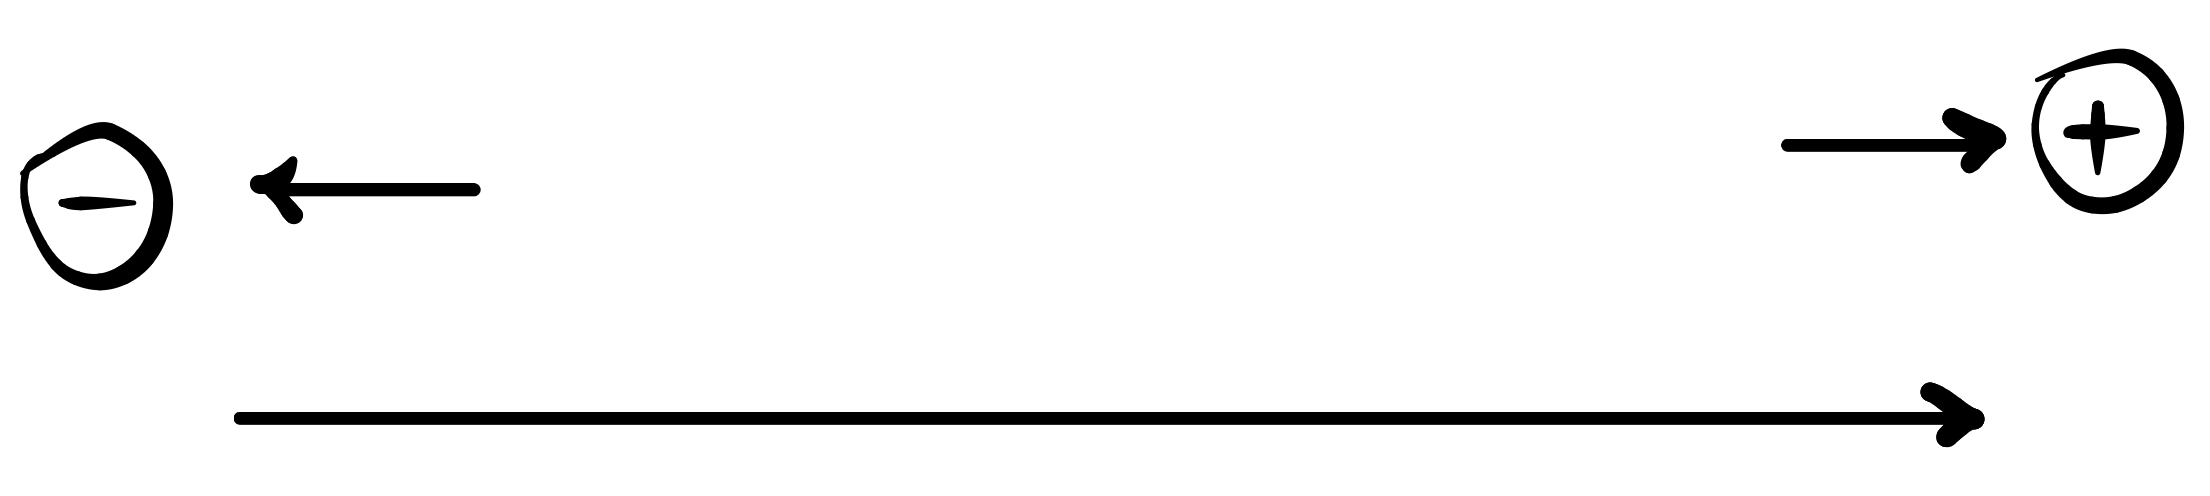
\includegraphics[scale=0.10]{imagenscinematicavetorial/grandezaescalar.jpeg}
    \caption{Em um movimento unidimensional a direção já está definida -- ela é única -- e o sentido pode ser expresso por dois sinais diferentes.}
    \label{fig_cinvet_grandezaescalar}
\end{figure}

Logo, se lhe for dito que um corpo possui velocidade de $-30$ km/h, você terá toda a informação necessária: você sabe a rapidez com que ele se move (valor absoluto da velocidade), você já sabe que ele se move na horizontal (direção do movimento) e, por conta do sinal, sabe que ele se move para a esquerda (sentido do movimento). Note que, para especificar com precisão para aonde um corpo se move, é fundamental saber essas três informações:

\begin{enumerate}
    \item [(i)] O valor absoluto da velocidade -- isso indica a rapidez com o corpo se move.
    \item [(ii)] A direção do movimento -- se ele ocorre na horizontal, na vertical, na diagonal, etc.
    \item [(iii)] O sentido do movimento: caso o movimento se dê na direção vertical, há duas possibilidades para o sentido: para cima ou para baixo. Se a direção for horizontal, o movimento pode ter sentido para direita ou para esquerda; etc.
\end{enumerate}


Perceba, contudo, que ao lhe informar que um corpo parte do ponto $P$ com velocidade de $30$ km/h, existem uma infinidade de movimentos possíveis, como mostra a primeira imagem da Figura \ref{fig_cinvet_grandezavetorial}: todas as direções são possíveis. Poderíamos especificar a direção, dizendo que é aquela que faz um ângulo de $60^\circ$ com a horizontal, como mostra a segunda imagem. Contudo, isso ainda seria insuficiente, posto que o corpo poderia se mover para um lado ou para o outro ao longo de tal direção -- ainda restariam duas opções possíveis.

\begin{figure}[h]
    \centering
    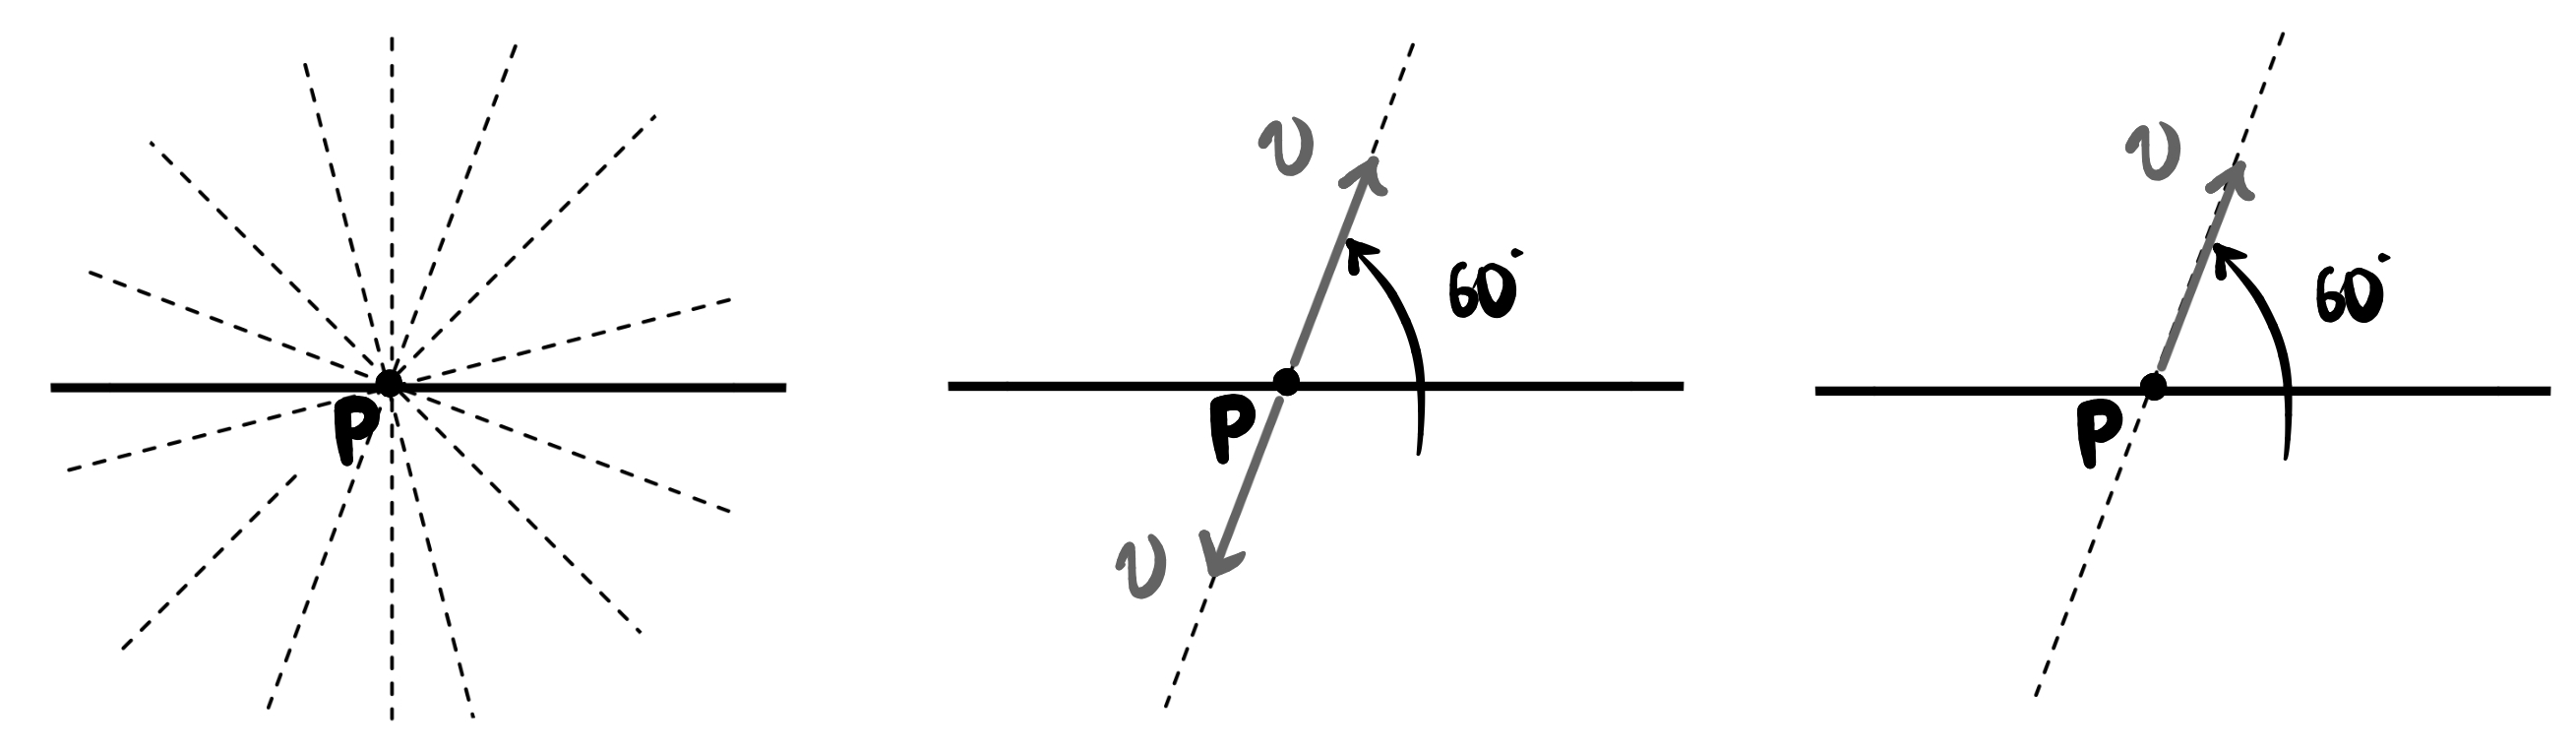
\includegraphics[scale=0.12]{imagenscinematicavetorial/grandezavetorial.jpeg}
    \caption{Para determinar com precisão o movimento é preciso informar o valor da velocidade, sua direção e seu sentido.}
    \label{fig_cinvet_grandezavetorial}
\end{figure}

Se afunilarmos e cravarmos que o corpo se move ``para cima'' -- ou seja, o sentido do movimento --, aí sim teremos transmitido toda a informação necessária para especificar o movimento -- a última imagem da Figura \ref{fig_cinvet_grandezavetorial} mostra isso.  \\



\begin{figure}[h]
    \centering
    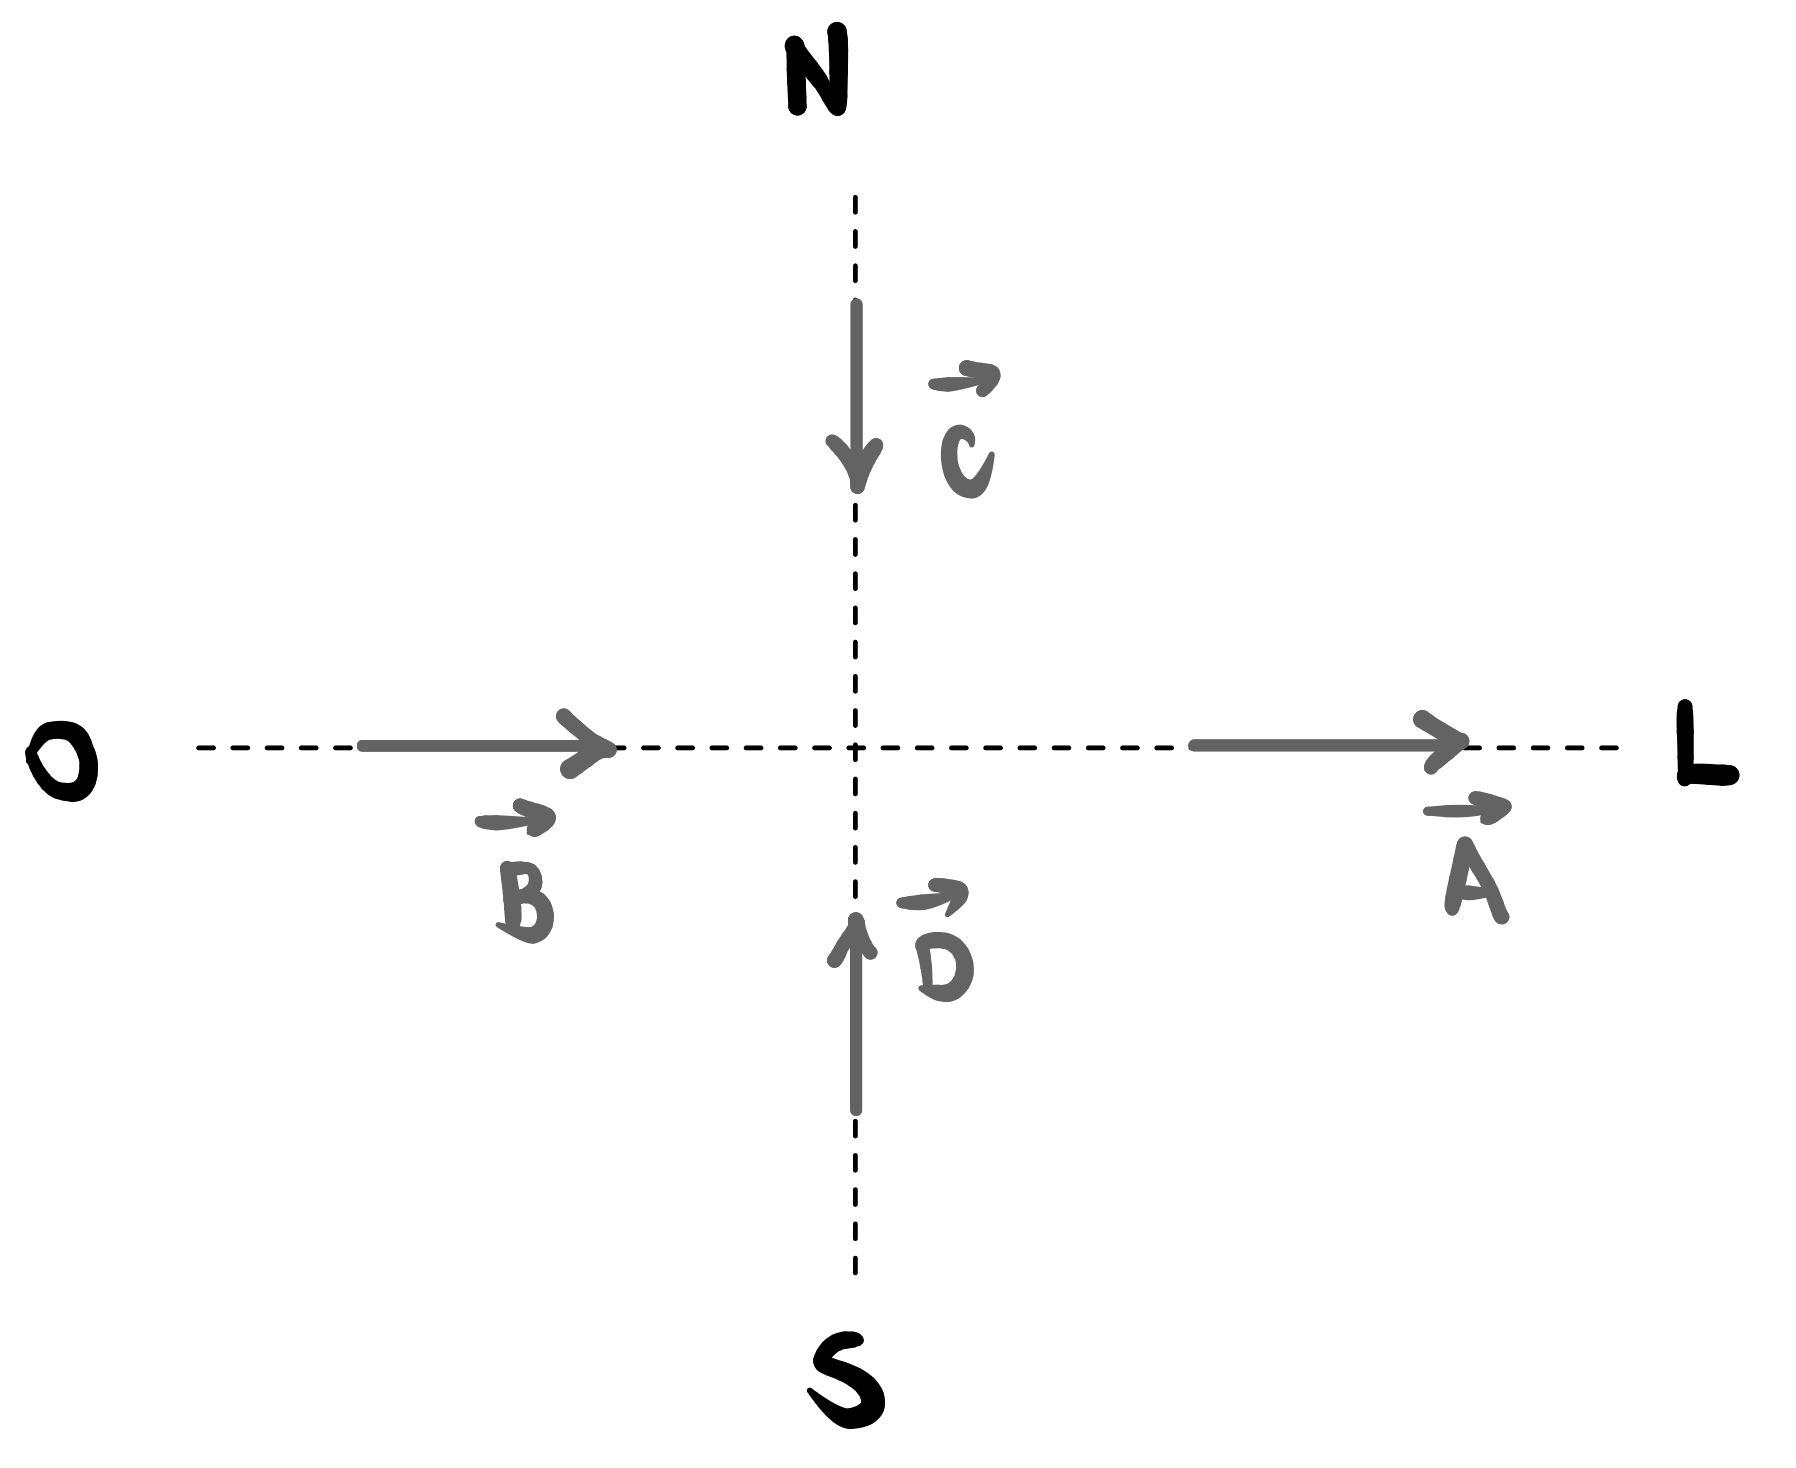
\includegraphics[scale=0.10]{imagenscinematicavetorial/vetordirecaosentido.jpeg}
    \caption{A diferença entre direção e sentido.}
    \label{fig_cinvet_vetordirecaosentido}
\end{figure}



Existem, portanto, certas grandezas que exigem que se informe não apenas seu valor, mas sua direção e sentido para que a informação transmitida esteja completa. Tais grandezas são chamadas de \textbf{grandezas vetoriais}, sendo a velocidade, a aceleração e a força alguns exemplos. Representaremos tais grandezas por setas, uma vez que uma seta consegue carregar essas três informações:

\begin{enumerate}
    \item [(i)] O valor da grandeza vetorial estará associado ao tamanho da seta. Logo, uma velocidade de $40$ km/h será representada por uma seta de tamanho $40$, enquanto uma velocidade de $20$ km/h será representada por uma seta com metade do tamanho. Chamamos isso de módulo do vetor e ele representa seu valor absoluto. Geometricamente, trata-se do tamanho da seta.
    \item [(ii)] A direção será determinada pela direção da seta\footnote{Que, normalmente, será especificada com base no ângulo que a seta faz com alguma direção -- normalmente, a horizontal.}. A Figura \ref{fig_cinvet_vetordirecaosentido} mostra, por exemplo, setas na direção vertical (norte-sul) e na direção horizontal (leste-oeste).
    \item [(iii)] Como uma seta pode apontar para dois sentidos diferentes em uma mesma direção, o sentido da seta irá indicar o sentido do vetor. No caso da Figura \ref{fig_cinvet_vetordirecaosentido} vemos que os vetores $\vec{A}$ e $\vec{B}$ possuem mesma direção (leste-oeste) e também o mesmo sentido: de oeste para leste (ou para a direita, caso prefira). Já os vetores $\vec{C}$ e $\vec{D}$ possuem a mesma direção (norte-sul, ou direção vertical), porém sentidos contrários.
\end{enumerate}







Representaremos uma grandeza vetorial, digamos, velocidade, por $\vec{v}.$ A seta em cima indica que se trata de um vetor. Perceba que a equação $\vec{v}=30$ km/h não faz sentido, porque estamos dizendo que uma seta -- um vetor -- é igual a um número, o que está claramente errado. Uma seta tem módulo, direção e sentido. O número, portanto, é só uma das características da seta -- está relacionada com o seu tamanho -- mas a seta é um ente geométrico que possui outras características além do tamanho.

Assim, para evitarmos esse tipo de incoerência, usaremos as seguinte notações quando quisermos nos referir ao tamanho do vetor, ou seja, seu módulo ou valor absoluto:

$$ v = |\vec{v}| = 30 \text{ km/h}.$$

Neste caso deixamos claro que estamos falando apenas de uma das características da seta: seu tamanho. A equação acima deve ser lida como \textit{o valor da velocidade é de 30 km/h} ou \textit{o módulo do vetor velocidade é de 30 km/h.} No caso da Equação \eqref{mecanica_eq_velocidaderelativa}, por exemplo, ela relaciona os \emph{módulos} das velocidades $v_A$ e $v_B$. Não introduzimos essa nomenclatura naquele contexto uma vez que a matemática dos vetores ainda não havia sido apresentada ao leitor.


Para lidar com movimentos que mudam de direção, movimentos curvilíneos e movimentos bidimensionais, de modo geral, o caráter vetorial de grandezas como velocidade ou aceleração será imprescindível. Desse modo, é importante que compreenda-se bem como funciona a matemática dos vetores.



\section{A Matemática dos Vetores}

Dentro do escopo do ensino médio existem essencialmente duas operações que podemos fazer com setas: multiplicar por uma constante (um escalar) ou somar/subtrair setas. Vamos entender em detalhes como funciona cada uma dessas operações.


\subsection{Multiplicação por Escalar}

Existem, além das grandezas vetoriais, as grandezas escalares. Enquanto os vetores precisam de módulo, direção e sentido para serem únicos, as grandezas escalares só precisam do módulo, isto é, do valor absoluto da grandeza. Um exemplo seria a temperatura. Se eu lhe disser que a temperatura ambiente está em $24^\circ$ Celsius você entendeu perfeitamente toda a informação necessária. A temperatura não aponta para lugar algum -- não precisa de direção ou sentido: é um escalar.

Grandezas escalares, portanto, são representadas apenas por um único número. Dito isso, nossa operação atual consiste em multiplicar um vetor por um escalar, ou seja, multiplicar um vetor por um número. O que essa operação faz é aumentar ou diminuir o tamanho de tal vetor, podendo, no máximo, inverter o seu sentido caso o número seja negativo.

A Figura \ref{fig_cinvet_multiplicarporescalar} mostra isso. Considere o vetor $\vec{A},$ que está na direção horizontal com sentido para a direita. Se multiplicarmos tal vetor por $2$ ou por $0,5$ teremos um vetor que terá, respectivamente, o dobro do tamanho e metade do tamanho do vetor $\vec{A};$ apontando, contudo, na mesma direção e sentido.

Poderíamos, contudo, multiplicar o vetor $\vec{A}$ por $-1$, o que nos daria um vetor de mesmo tamanho, mesma direção, porém sentido oposto. Já o vetor $-2\vec{A}$ possui a mesma direção, o dobro do tamanho e o sentido contrário ao de $\vec{A}.$


\begin{figure}[h]
    \centering
    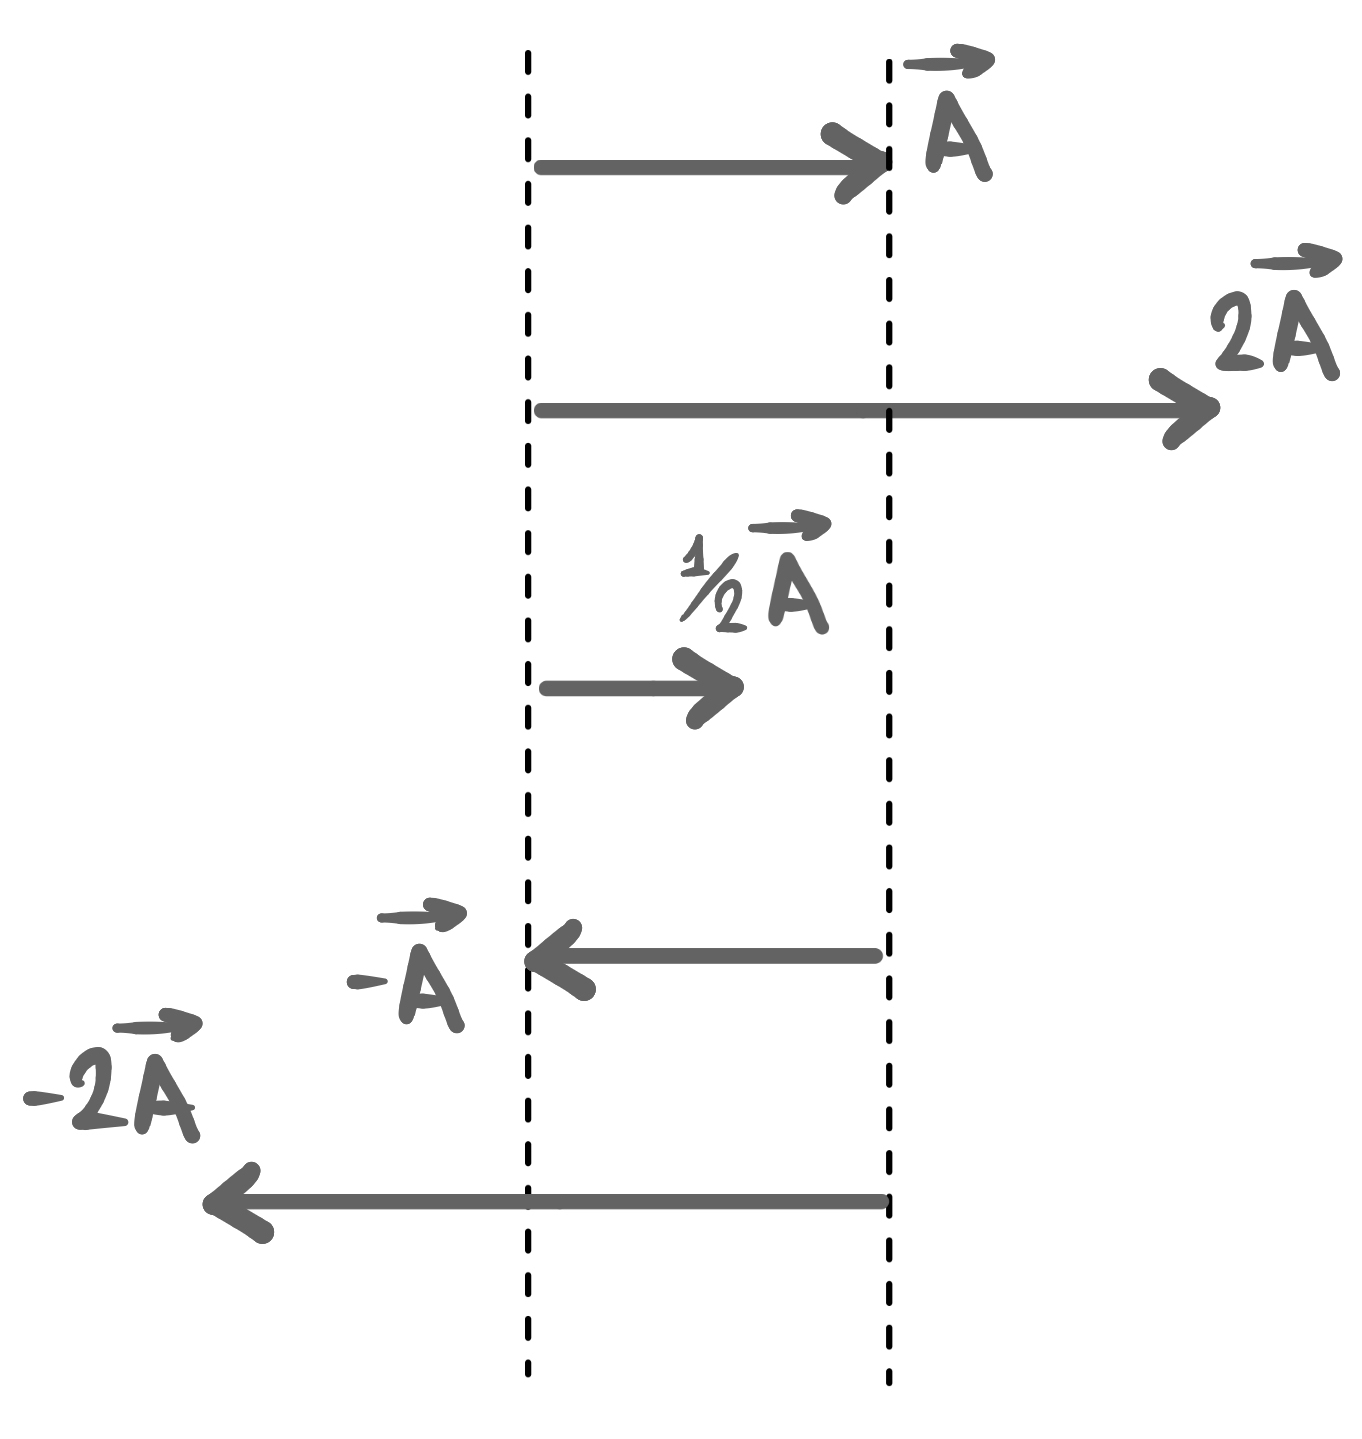
\includegraphics[scale=0.12]{imagenscinematicavetorial/dilatacaovetor.jpeg}
    \caption{A multiplicação de um vetor por um escalar.}
    \label{fig_cinvet_multiplicarporescalar}
\end{figure}


Note, portanto, que o efeito da multiplicação de um vetor por um escalar é o de dilatar ou contrair tal vetor: se o número for maior que $1$ (ou menor que $-1)$ nós estaremos aumentando o tamanho do vetor por tal fator multiplicativo. Já se o número for algo entre $0$ e $1$ (ou entre $-1$ e $0$) nós estaremos contraindo o vetor por tal fator multiplicativo. Além disso, tal operação permite que o sentido do vetor seja invertido -- caso o fator multiplicativo seja negativo -- mas nunca altera a direção original do vetor.



\subsection{Soma e Subtração}

Somar setas pode parecer uma operação estranha em um primeiro momento, mas veremos que ela é bem intuitiva. Imagine, como mostra a Figura \ref{fig_cinvet_somavetoresintro}, que você vai se deslocar do ponto $1$ até o ponto $2$ no espaço. Chegando no ponto $2,$ você se desloca até o ponto $3.$ Chegando lá, você vai para o ponto $4$ e, por fim, se desloca do ponto $4$ ao $5.$


\begin{figure}[h]
    \centering
    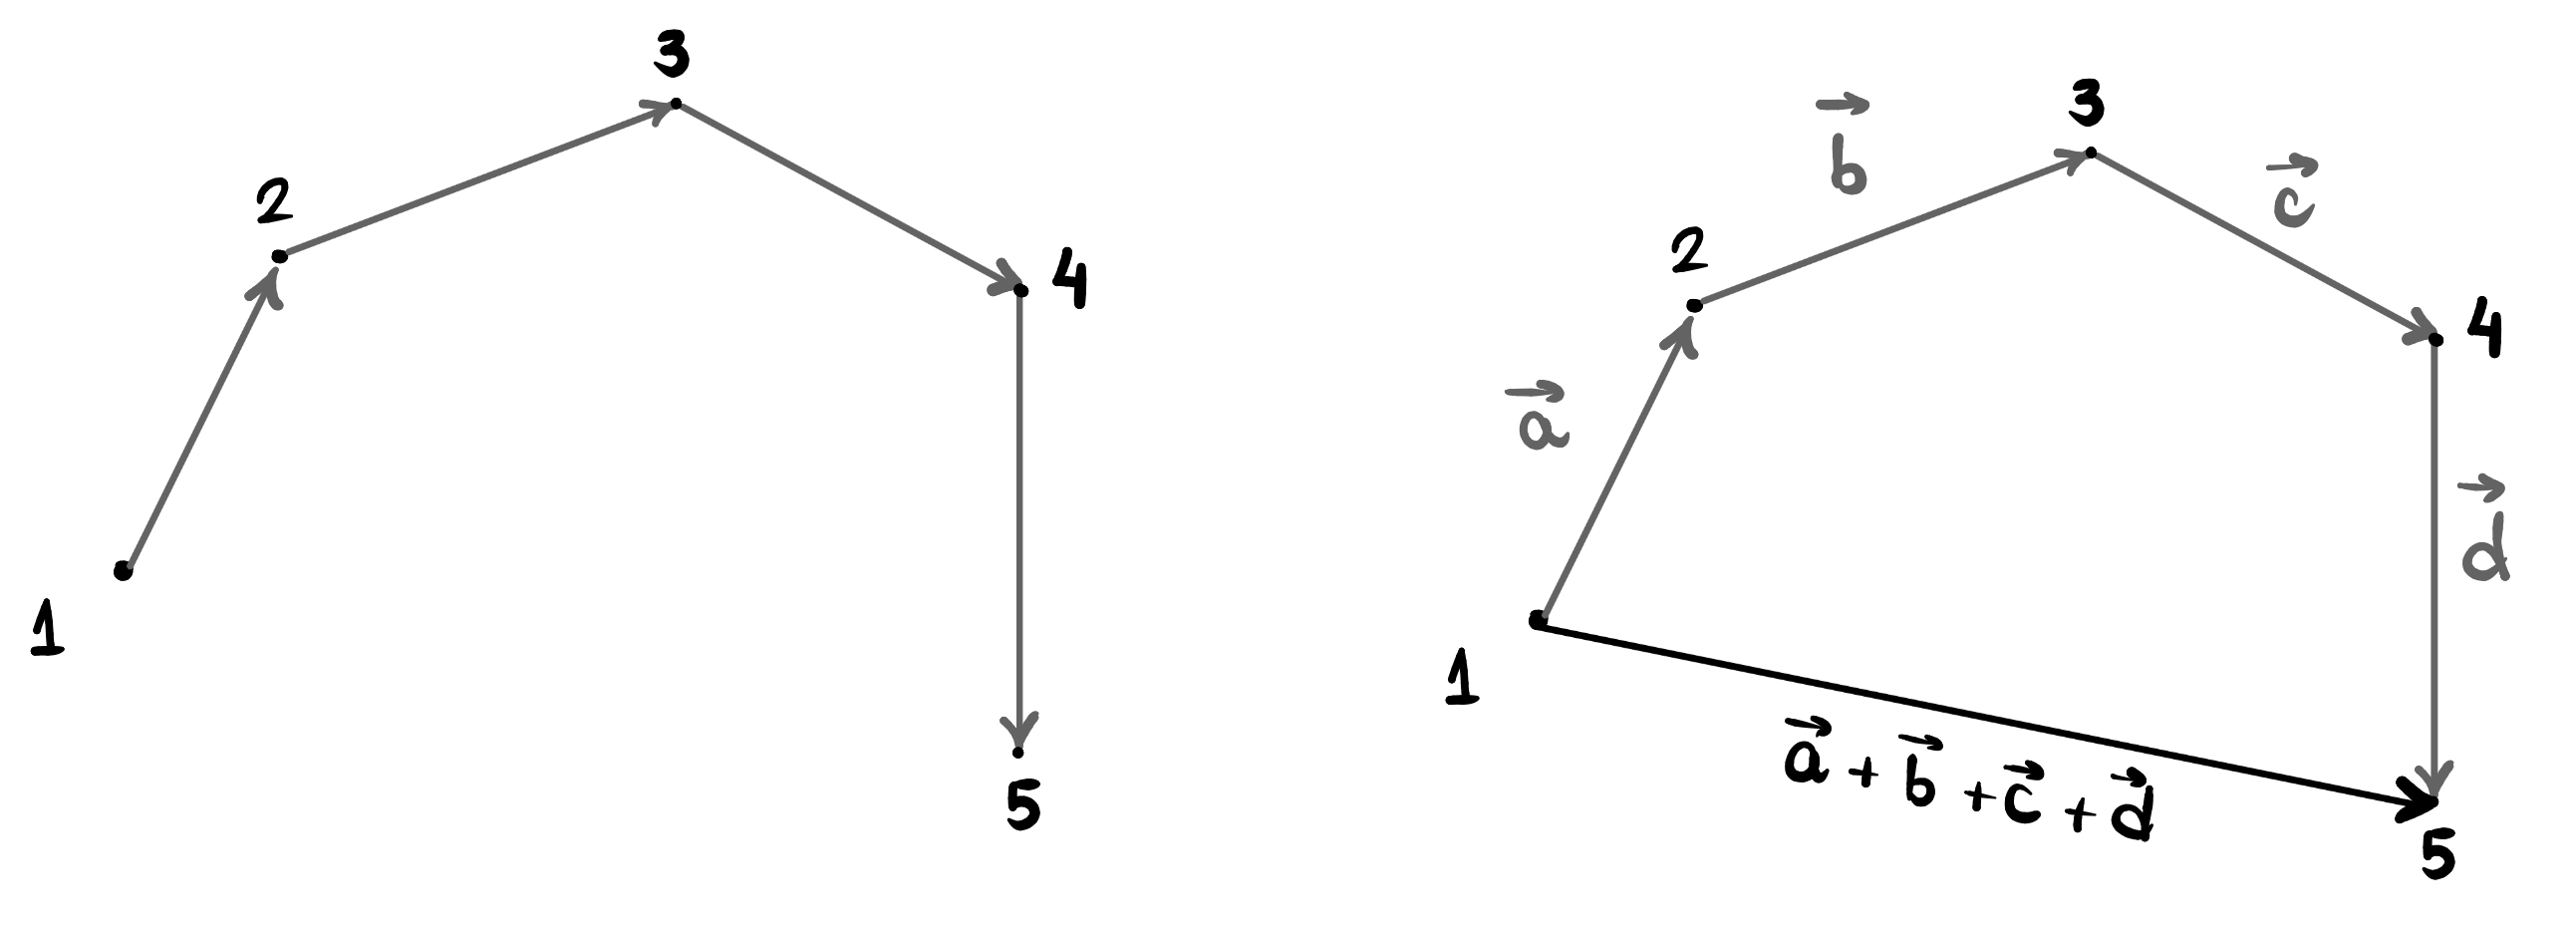
\includegraphics[scale=0.12]{imagenscinematicavetorial/somarsetasintro.jpeg}
    \caption{A soma dos vetores $\vec{a},\vec{b}, \vec{c} $ e $\vec{d}.$}
    \label{fig_cinvet_somavetoresintro}
\end{figure}

Temos aqui quatro setas que representam cada deslocamento que você teve ao longo do movimento. Como podemos somá-las? Ora, o efeito total do seu movimento foi sair do ponto $1$ e chegar ao ponto $5,$ desse modo, seu deslocamento total -- o quanto você se distanciou do ponto de partida -- é representado pela seta que une o ponto de partida (ponto $1)$ ao ponto de chegada (ponto $5$). Pronto: você acabou de aprender a lógica que guia a soma de setas.

De forma mais matemática, se os vetores em questão forem designados por $\vec{a},\vec{b}, \vec{c} $ e $\vec{d},$ o vetor soma $(\vec{a}+\vec{b}+\vec{c} +\vec{d})$\footnote{É importante que o leitor perceba a diferença entre a operação $(\vec{a}+\vec{b}+\vec{c} +\vec{d})$ e a operação $a+b+c+d$: a primeira envolve a soma de setas, enquanto a segunda envolve a soma de números -- que representam o tamanho das setas. Mais adiante vamos destacar com ainda mais ênfase essa diferença.} é aquele representado na segunda imagem da Figura \ref{fig_cinvet_somavetoresintro}.

A regra, portanto, é: para somar duas setas, conecte o início de uma delas com a extremidade da outra. A seta resultante é aquela que vai do início da primeira à extremidade da última. Isso vale para duas, três, cinco ou quarenta setas (vetores) que quisermos somar. Algumas perguntas poderiam surgir neste momento:

\begin{enumerate}
    \item [(i)] \textit{Mas e se os vetores em questão não forem referentes a um deslocamento?}

    Não mudaria nada. A lógica para se somar setas é sempre a mesma. Usamos os vetores $\vec{a},\vec{b}, \vec{c} $ e $\vec{d}$ como se fossem deslocamentos para deixar mais intuitivo a razão de essa ser a regra para se somar setas. Contudo, se os vetores $\vec{a},\vec{b}, \vec{c} $ e $\vec{d}$ representassem velocidades, acelerações ou forças, a operação de somá-los se daria exatamente do mesmo modo.
    
    \item [(ii)] \textit{Como poderíamos saber o tamanho do vetor resultante no caso da Figura \ref{fig_cinvet_somavetoresintro} ?}

    Essa seria uma ótima pergunta. O que se quer saber é, sabendo quais são os tamanhos das setas $\vec{a},\vec{b}, \vec{c} $ e $\vec{d}$, como podemos obter o tamanho da seta final? Essa será a pauta da nossa próxima discussão.
\end{enumerate}


Vamos à nobre tarefa de somar duas setas, digamos, $\vec{A}$ e $\vec{B},$ cujos tamanhos são 4 e 3, respectivamente. Ou seja, em notação matemática:

 $$|\vec{A}|=4 \quad \text{ e } \quad |\vec{B}|=3. $$

O leitor menos atento já poderia concluir que o vetor soma $(\vec{A}+\vec{B})$ será uma seta de tamanho $(4+3)=7,$ o que seria precipitado e, provavelmente, incorreto. Perceba que o tamanho da seta resultante irá depender das direções de cada uma das setas que serão somadas e, para cada uma delas, a geometria da soma será diferente. 

A nossa regra para somar os vetores será desenhá-los de modo que o início de um deles coincida com a extremidade do outro e, a partir disso, o vetor resultante será aquele que vai do início do primeiro à extremidade do último. Veja o resultado que tal regra nos daria no caso da Figura \ref{fig_cinvet_somasetas01}\footnote{Uma seta não possui lugar fixo no espaço, de modo que o leitor tem liberdade de desenhá-la aonde ele quiser: desde que possua o mesmo módulo, mesma direção e mesmo sentido, tratar-se-á sempre do mesmo vetor, independente da posição em que ele está desenhado.}.

Na primeira imagem temos os vetores $\vec{A}$ e $\vec{B},$ na imagem do meio temos eles desenhados de modo que o início de um deles coincida com a extremidade do outro, e na terceira imagem temos a regra da soma aplicada: o vetor soma é o que vai da origem do primeiro à extremidade do último. Note que, neste caso, sendo os tamanhos dos vetores $\vec{A}$ e $\vec{B}$ iguais a $4$ e $3,$ o nosso vetor soma terá, de fato, um tamanho que é igual à soma dos tamanhos dos vetores somados: $4+3=7.$


\begin{figure}[h]
    \centering
    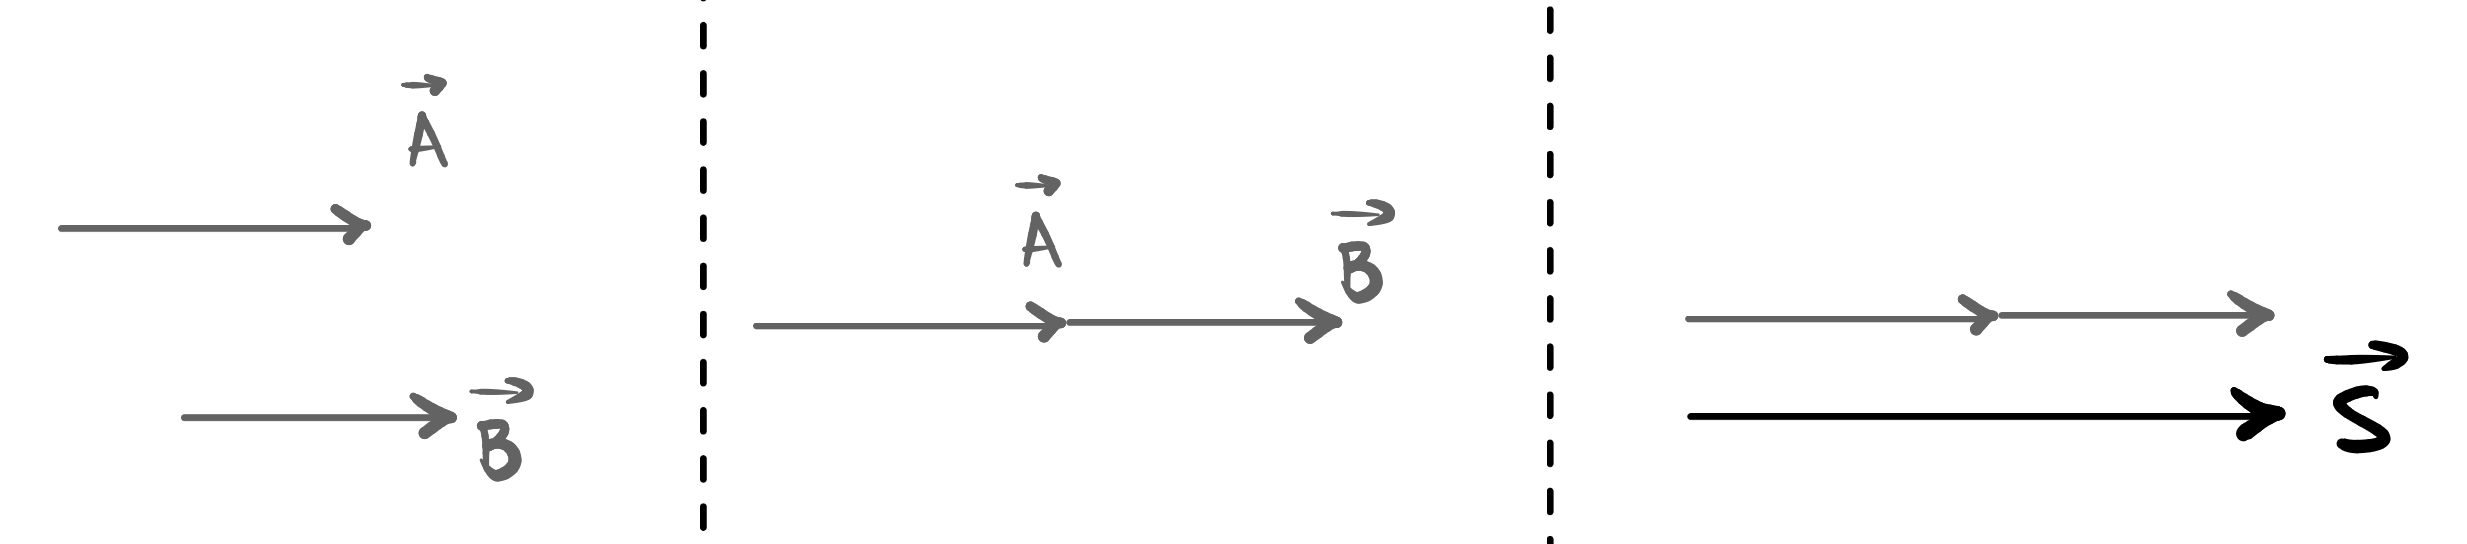
\includegraphics[scale=0.12]{imagenscinematicavetorial/somarvetores1.jpeg}
    \caption{Somando os vetores $\vec{A}$ e $\vec{B}$ de mesma direção e sentido.}
    \label{fig_cinvet_somasetas01}
\end{figure}

Perceba, contudo, os mesmos vetores $\vec{A}$ e $\vec{B}$ de tamanhos $4$ e $3,$ porém de sentidos opostos, como no contexto da Figura \ref{fig_cinvet_somasetas02}.


\begin{figure}[h]
    \centering
    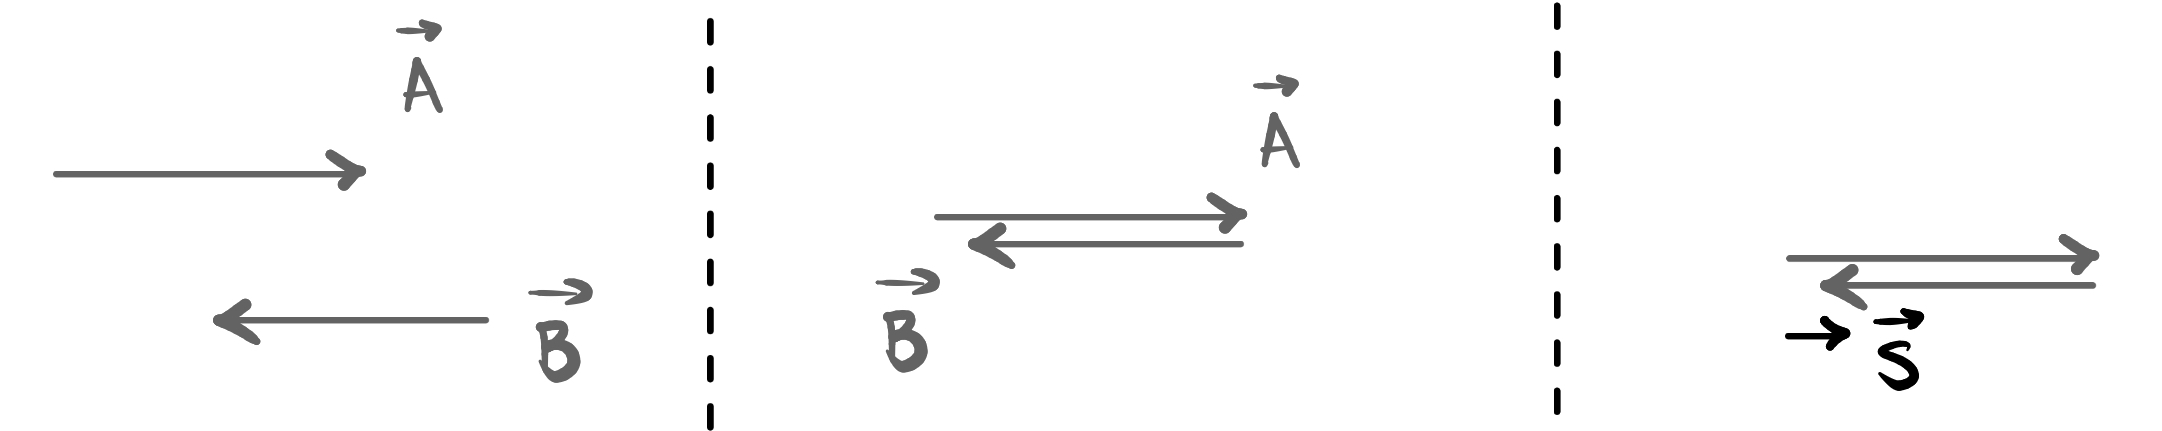
\includegraphics[scale=0.135]{imagenscinematicavetorial/somarvetores2.jpeg}
    \caption{Somando os vetores $\vec{A}$ e $\vec{B}$ de mesma direção e sentidos opostos.}
    \label{fig_cinvet_somasetas02}
\end{figure}


Neste caso, o vetor que vai da origem de $\vec{A}$ até a extremidade de $\vec{B}$ terá um tamanho dado por $4-3=1,$ como mostra a geometria da situação na Figura \ref{fig_cinvet_somasetas02}.

Já se alterarmos as direções dos vetores $\vec{A}$ e $\vec{B}$ para a situação da Figura \ref{fig_cinvet_somasetas03}, em que tais vetores tenham direções perpendiculares, notaremos agora que o tamanho da seta resultante será dado pelo Teorema de Pitágoras, ou seja, será igual a

$$ \sqrt{3^2+4^2}=5.$$

\begin{figure}[h]
    \centering
    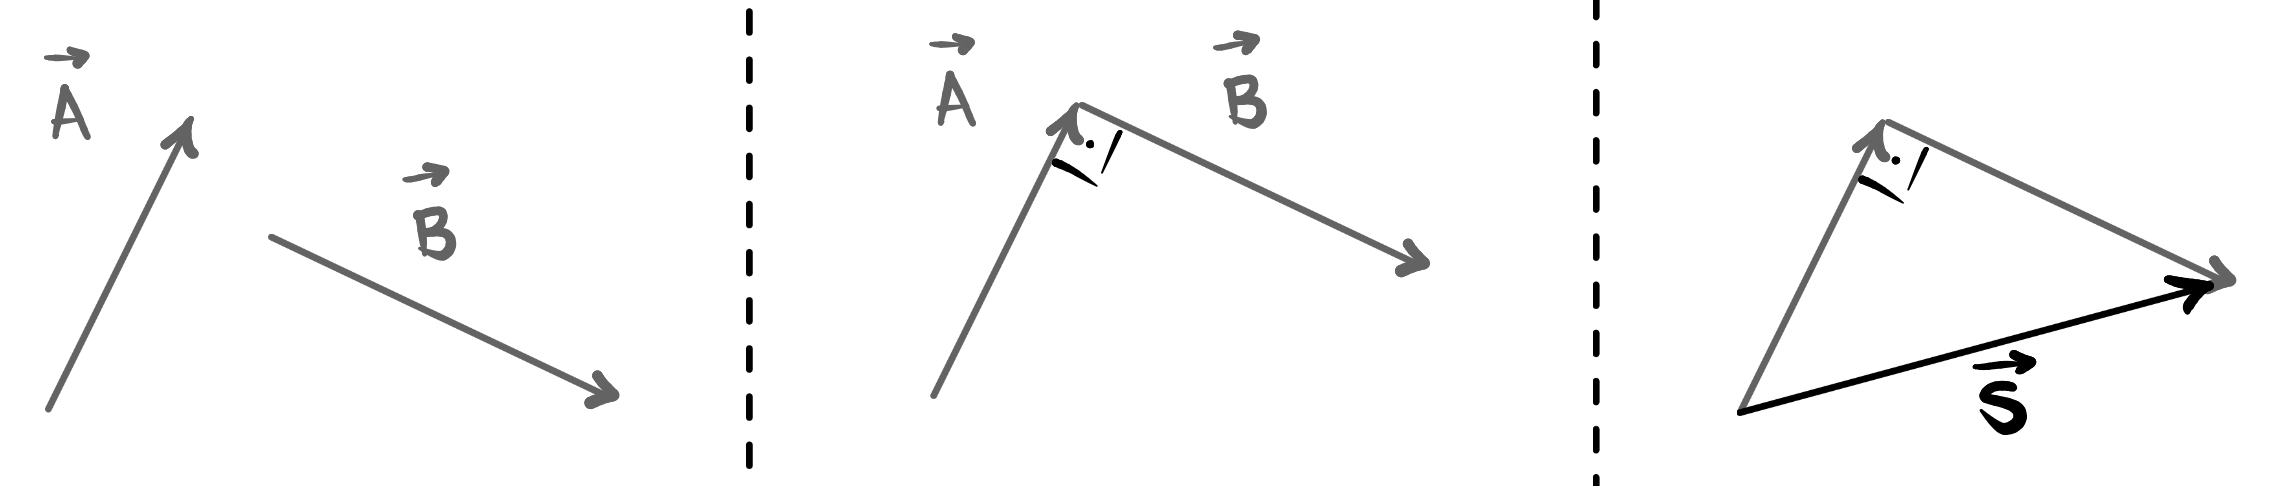
\includegraphics[scale=0.12]{imagenscinematicavetorial/somarvetores3.jpeg}
    \caption{Somando os vetores $\vec{A}$ e $\vec{B}$ de direções perpendiculares.}
    \label{fig_cinvet_somasetas03}
\end{figure}

Por fim, se as direções dos vetores $\vec{A}$ e $\vec{B}$ fizerem um ângulo de $120$ graus, como mostra a Figura \ref{fig_cinvet_somasetas04}, ao aplicar a mesma regra de soma, seremos levados a uma geometria que nos obrigaria a aplicar a Lei dos Cossenos, que forneceria como resultado que o tamanho da seta resultante da soma das setas $\vec{A}$ e $\vec{B}$ seria

$$ \sqrt{3^2+4^2- 2 \cdot 4\cdot 3 \cdot \cos(120^\circ)} = \sqrt{37} \approx 6{,}08. $$

\begin{figure}[h]
    \centering
    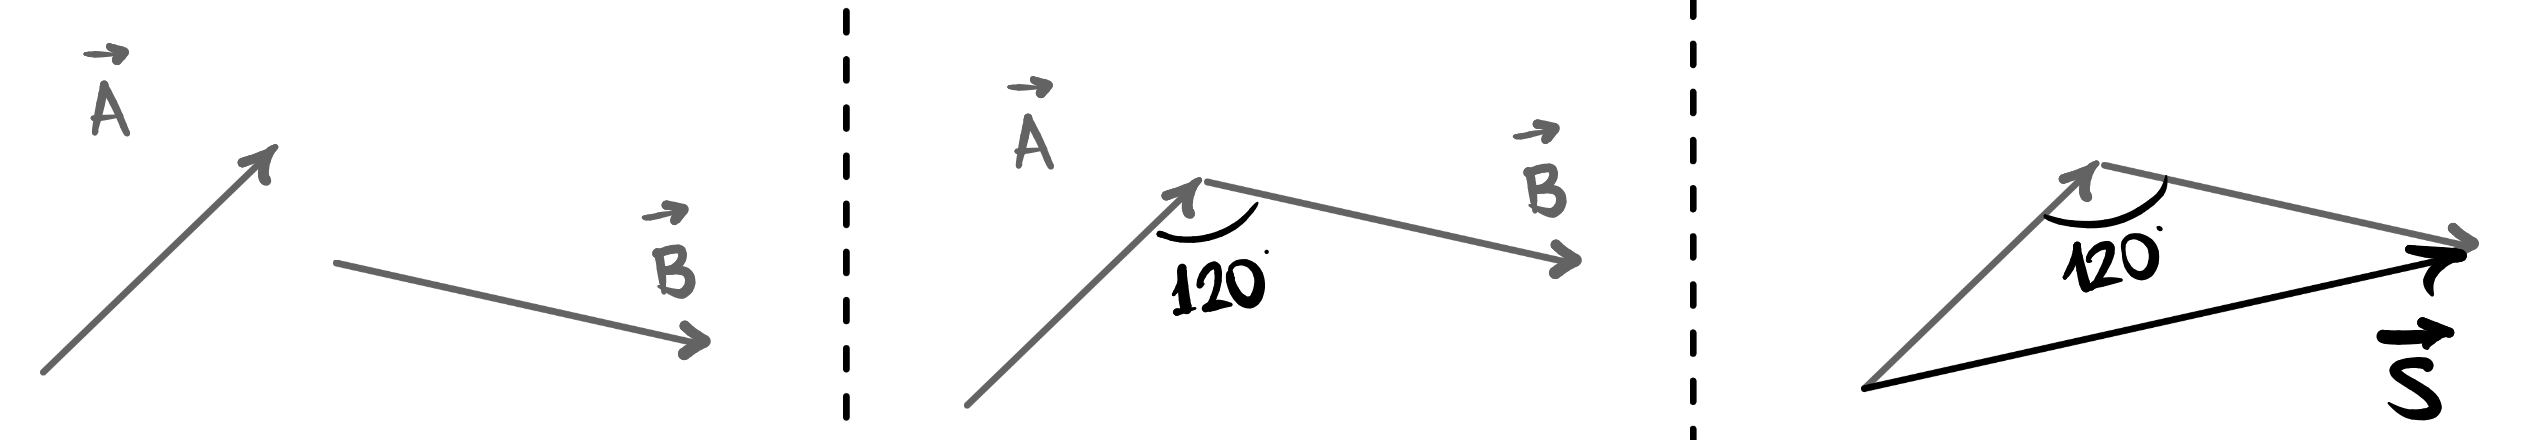
\includegraphics[scale=0.12]{imagenscinematicavetorial/somarvetores4.jpeg}
    \caption{Somando os vetores $\vec{A}$ e $\vec{B}$ de direções que fazem um ângulo obtuso.}
    \label{fig_cinvet_somasetas04}
\end{figure}



Sendo assim, o problema de obter o tamanho da seta resultante a partir da soma de outras duas setas é um problema de geometria. Para cada direção e sentido das setas somadas a geometria será uma, de modo que, para setas, $3+4$ nem sempre dá $7.$ 

Como vimos, é possível somar setas de tamanhos $3$ e $4$ e obter como resultado uma seta cujo tamanho dá $1$, ou $5$, ou $6{,}08$ ou até mesmo o próprio $7.$ Ao somar vetores de módulos $3$ e $4$ poderemos obter, para o tamanho do vetor resultante, qualquer valor entre $1$ e $7$ -- os casos das Figuras \ref{fig_cinvet_somasetas01} e \ref{fig_cinvet_somasetas02} são os extremos. Quando as setas possuem a mesma direção e mesmo sentido teremos um valor máximo para o tamanho da seta resultante; já quando elas possuem mesma direção e sentidos opostos teremos um valor mínimo para o tamanho da seta resultante. Qualquer outra configuração geométrica diferente dessas fornecerá um valor de tamanho para a seta resultante entre $1$ e $7.$


Logo, olhando para a situação da Figura \ref{fig_cinvet_somavetoresintro}, é impossível sabermos o tamanho da seta resultante sem sabermos exatamente o tamanho e os ângulos que as setas $\vec{a},\vec{b}, \vec{c} $ e $\vec{d}$ fazem entrem si, uma vez que são eles que definem a geometria do problema.


Por fim, vamos comentar sobre a operação de subtrair setas. Digamos que queremos fazer a subtração do vetor $\vec{B}$ do vetor $\vec{A},$ isto é, computar $(\vec{A}-\vec{B})$. Ora, note que isso é o mesmo que somar o vetor $\vec{A}$ com o vetor $-\vec{B},$ ou seja:

$$ \vec{A}-\vec{B} = \vec{A} + (- \vec{B}),$$

\noindent ou seja, uma vez que sabemos que $-\vec{B}$ é simplesmente o vetor $\vec{B}$ apontando no sentido oposto, acabamos de converter a subtração em uma soma: fazer a subtração $(\vec{A}-\vec{B})$ é somar o vetor $\vec{A}$ com o oposto do vetor $\vec{B},$ isto é, com $-\vec{B}$. A Figura \ref{fig_cinvet_subtrairsetas} mostra, na primeira coluna, a operação da soma dos vetores $\vec{A}$ e $\vec{B}$, enquanto a segunda coluna mostra a diferença entre os vetores.

\begin{figure}[h]
    \centering
    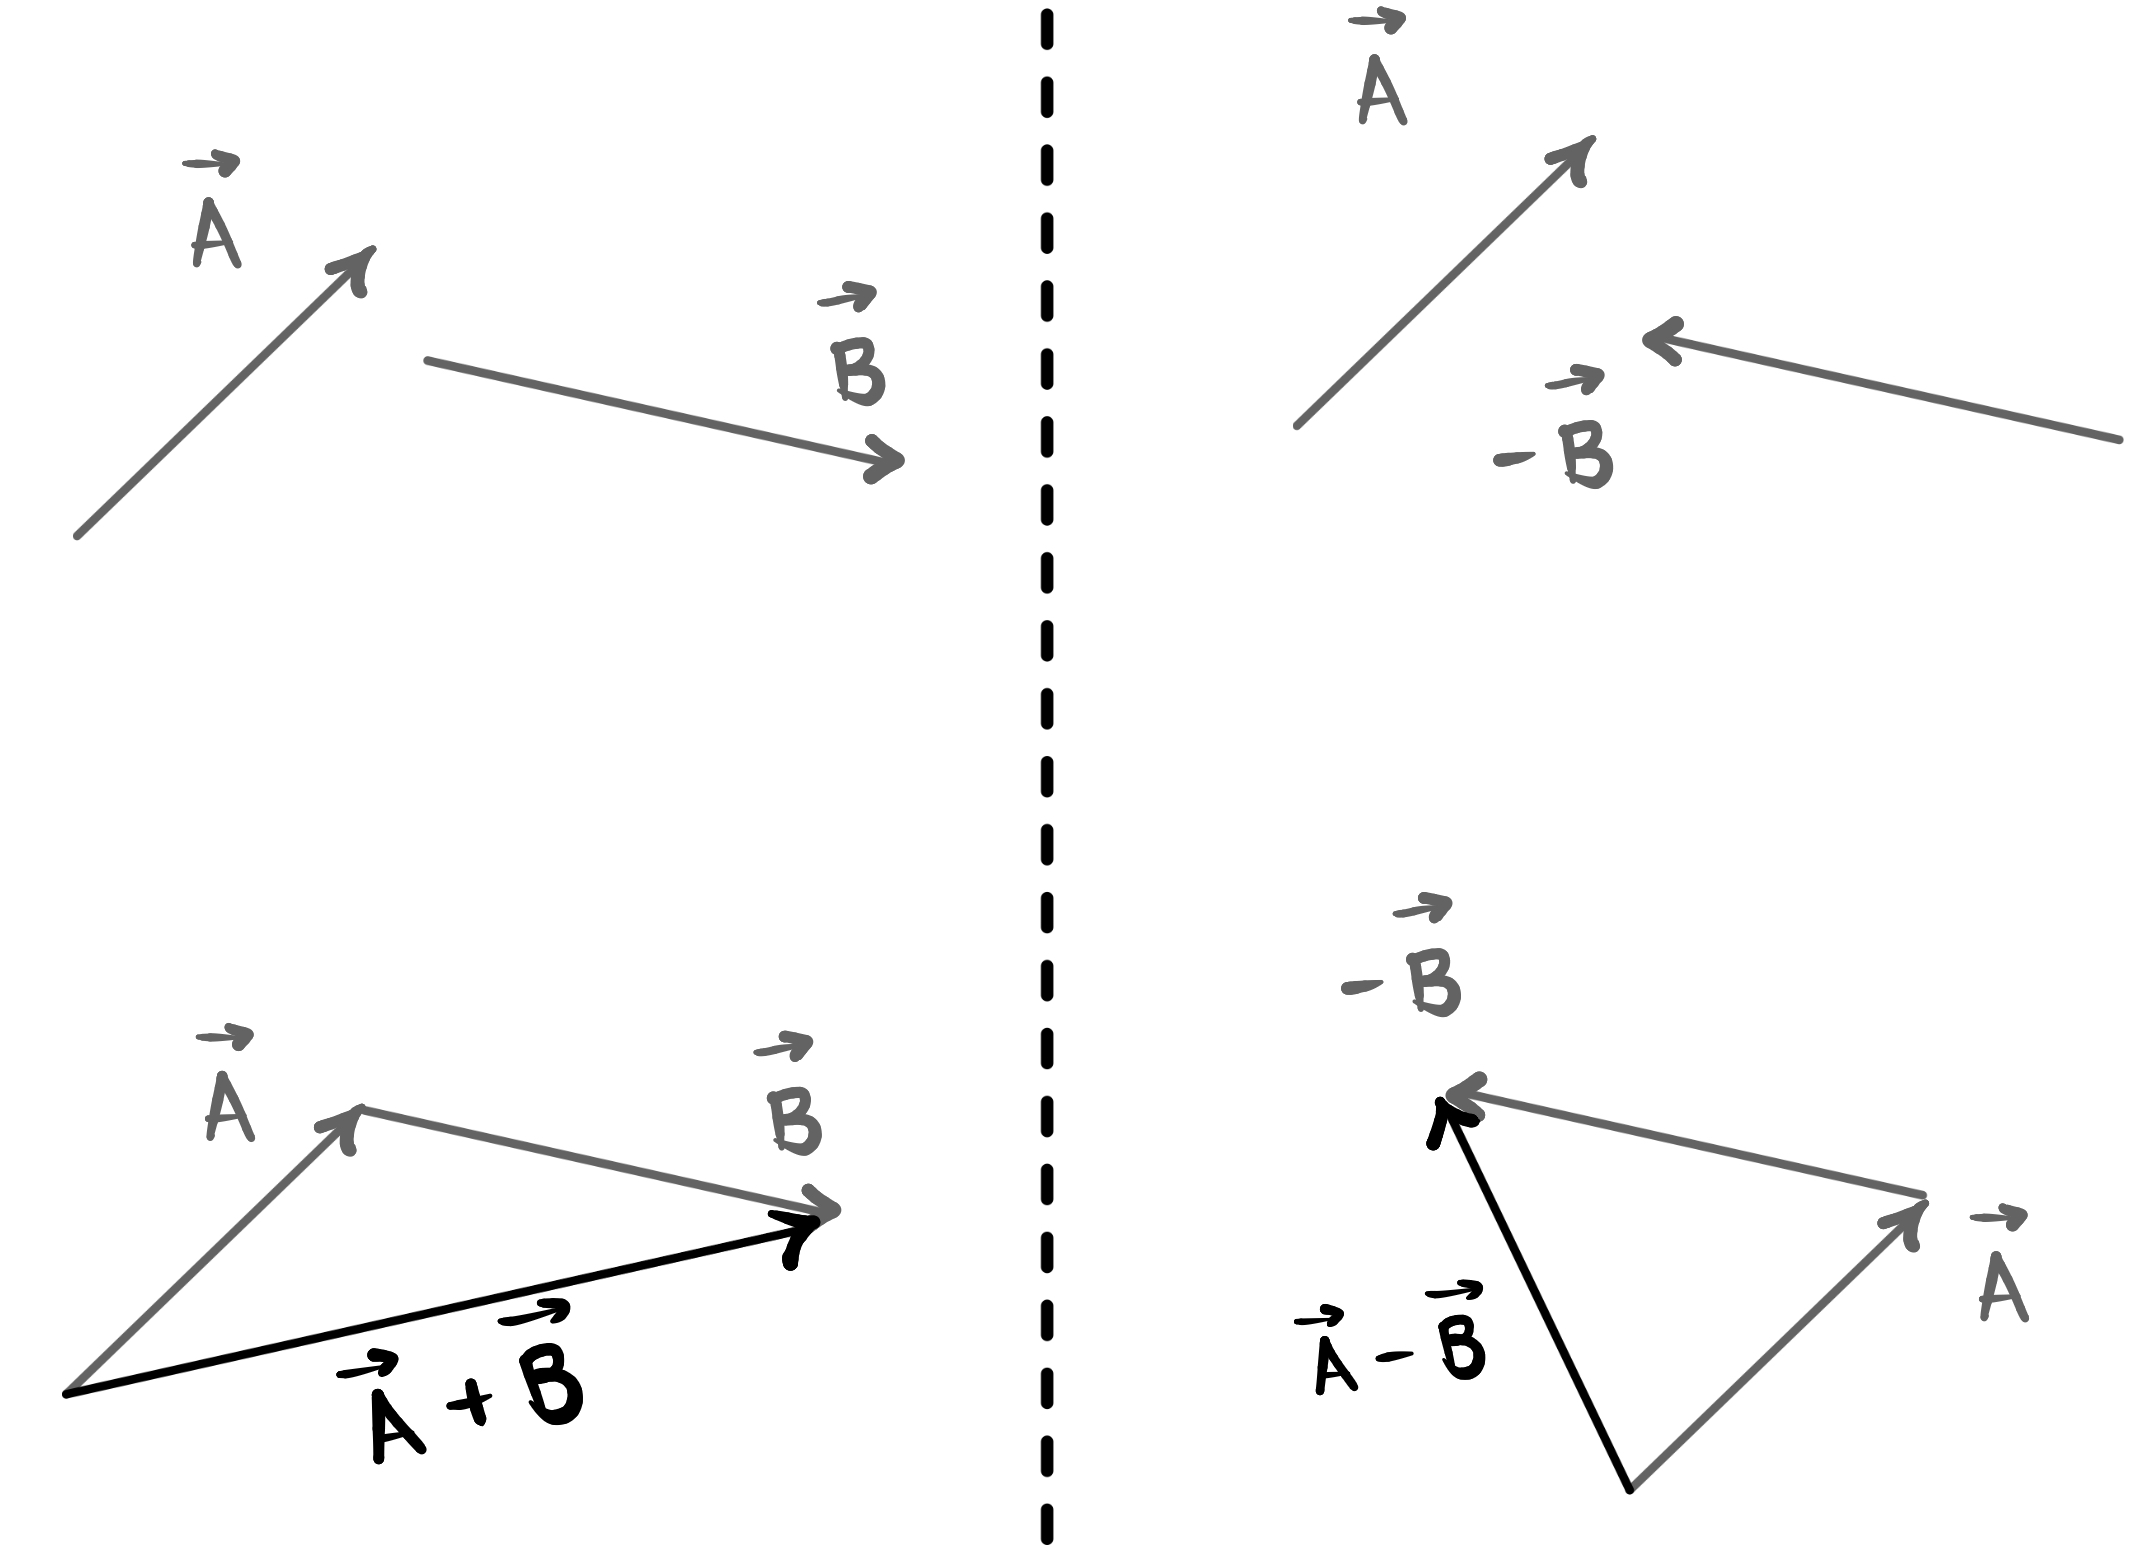
\includegraphics[scale=0.12]{imagenscinematicavetorial/subtrairvetores.jpeg}
    \caption{A soma e a subtração dos vetores $\vec{A}$ e $\vec{B}.$}
    \label{fig_cinvet_subtrairsetas}
\end{figure}


Curiosamente uma operação muito comum de se fazer com setas é o inverso do que construímos anteriormente. Ou seja, ao invés de lhe dar dois vetores e perguntar qual é o vetor resultante; teremos um único vetor e vamos querer entender quais são os outros dois vetores que, somados, dão ele.

É como se, em uma direção, estivéssemos fazendo a soma de $3+4,$ que naturalmente dá $7$ (estamos pensando em apenas números agora). Porém, neste momento, seremos apresentados ao número $7$, e buscaremos entender quais são os números que somados resultam nele. Perceba que essa pergunta pode ter várias respostas, dependendo do campo numérico que estivermos considerando. Ou seja, dado o número $7$, os dois números somados que resultam nele podem ser:

\begin{enumerate}
    \item [(i)] $3$ e $4$ caso estejamos restritos ao campo dos números naturais.
    \item [(ii)] $-5$ e $12$ caso ampliemos nosso escopo para os números inteiros (que incluem os negativos). Neste caso já teríamos várias outras possibilidades, como $-1$ e $8$ ou $-2$ e $9,$ por exemplo.
    \item [(iii)] $5.5$ e $1.5$ caso ampliemos nosso escopo para os números racionais (que incluem as frações). Neste também teríamos várias outras possibilidades, como $3.5$ e $3.5$ ou $-1.5$ e $8.5$, por exemplo.
\end{enumerate}

Perceba, portanto, que quando se somam dois números (ou duas setas) a resposta é única; porém, ao lhe ser entregue um número (ou uma seta), existirão várias possibilidades de pares de números (ou de setas) que, somados, dão como resultado o primeiro número.

No caso dos vetores, a ambiguidade tem a ver com a direção a ser escolhida para os vetores que, somados, darão o primeiro. Considere a Figura \ref{fig_cinvet_decomporvetores1}, que mostra, na primeira imagem, um dado vetor $\vec{A}.$ Queremos achar os dois vetores que, somados, resultam no vetor $\vec{A.}$ Na segunda imagem da figura foi fixada duas direções perpendiculares $x$ e $y$ -- as direções horizontal e vertical, respectivamente. Neste caso, fixadas essas direções, nossa resposta será única -- é como se estivéssemos nos restringindo ao campo dos números naturais, pensando em soma de números. Ou seja, a pergunta agora não é \textit{quais são os dois vetores que, somados, resultam no vetor A?}, mas sim \textit{quais são os dois vetores -- estando cada um deles nas direções $x$ e $y$ escolhidas -- que, somados, resultam no vetor A?}.


\begin{figure}[h]
    \centering
    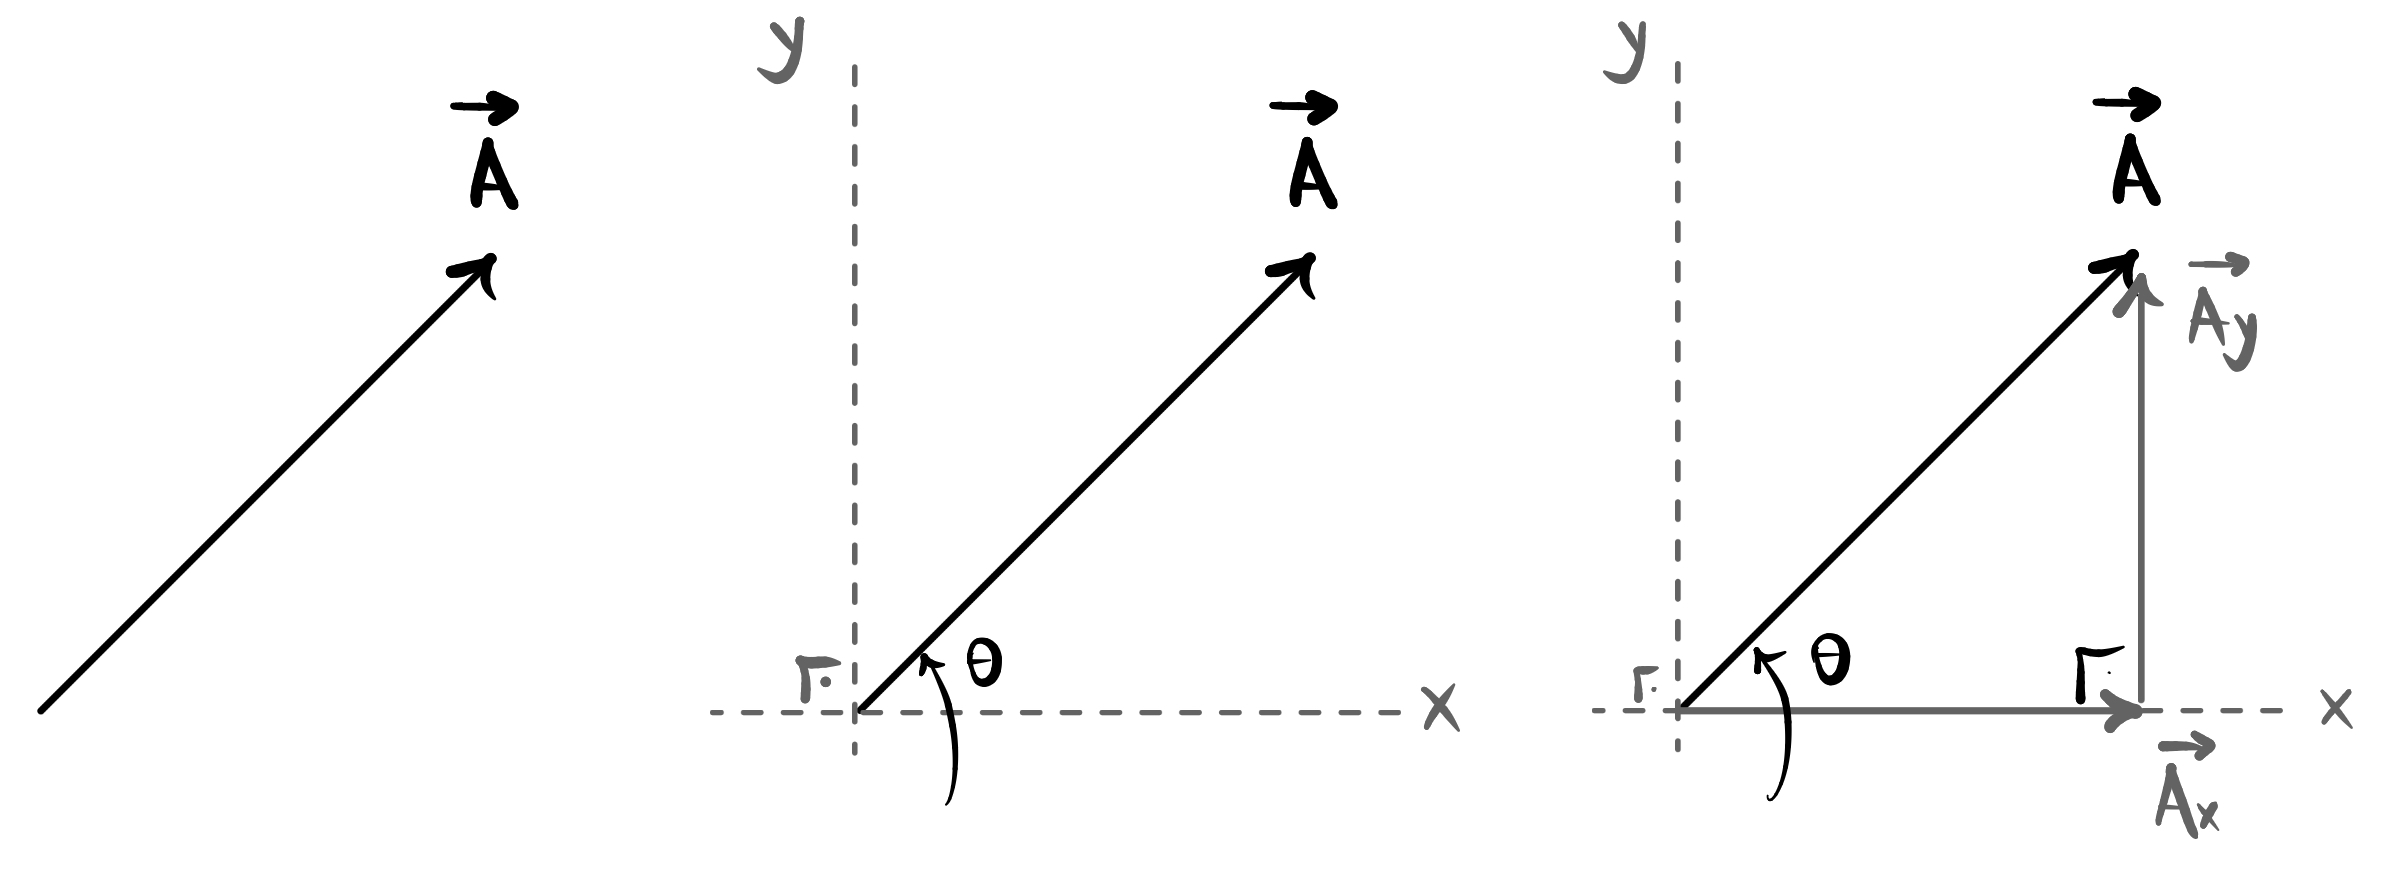
\includegraphics[scale=0.15]{imagenscinematicavetorial/decomporvetores1.jpeg}
    \caption{A decomposição vetorial nas direções cartesianas horizontal e vertical.}
    \label{fig_cinvet_decomporvetores1}
\end{figure}


Perceba, na última imagem, que os vetores $\vec{A}_x$ e $\vec{A}_y$, se somados, resultam no vetor $\vec{A},$ isto é:

$$ \vec{A} = \vec{A}_x + \vec{A}_y, $$

\noindent como queríamos. Ou seja, dado um vetor $\vec{A}$ encontramos os dois vetores $\vec{A}_x$ e $\vec{A}_y$ que, somados, resultam nele. Sendo as direções $x$ e $y$ perpendiculares, os módulos de tais vetores podem ser relacionados pelo Teorema de Pitágoras, isto é

$$ A^2 = A_x^2 + A_y^2,$$

\noindent e essa é a principal razão de se escolher direções perpendiculares -- para que valha o Teorema de Pitágoras na relação entre os módulos dos vetores. Poderíamos também relacionar o módulo de cada novo vetor $A_x$ e $A_y$ com o módulo $A$ do vetor inicial e o ângulo $\theta$ que ele faz com uma das direções escolhidas. Isso é feito usando a definição das razões trigonométricas no triângulo retângulo da terceira imagem da figura, de onde tiramos que

$$ \sin \theta = \dfrac{A_y}{A} \implies \boxed{A_y = A \sin \theta} \quad  \text{ e } \quad \cos \theta = \dfrac{A_x}{A} \implies \boxed{A_x = A \cos \theta.} $$

Esse é mais um motivo para usarmos direções perpendiculares na decomposição dos vetores: as relações trigonométricas acima são definidas e, portanto, só valem em triângulos retângulos.

O que acabamos de fazer foi uma \textbf{decomposição vetorial}: dado um vetor $\vec{A}$ e duas direções $x$ e $y$ encontramos quem são os vetores $A_x$ e $A_y$ ao longo de tais direções que, somados, resultam no vetor inicial $\vec{A}.$ Por isso, os vetores $\vec{A}_x$ e $\vec{A}_y$ são chamados de componentes do vetor $\vec{A.}$

Perceba que, se soubermos o módulo $A$ do vetor inicial $\vec{A}$ e qual é o ângulo $\theta$ que ele faz com alguma das direções escolhidas, as equações acima nos permitem calcular o módulo das suas componentes $A_x$ e $A_y$ e, portanto, resolver o problema proposto inicialmente.

\begin{figure}[h]
    \centering
    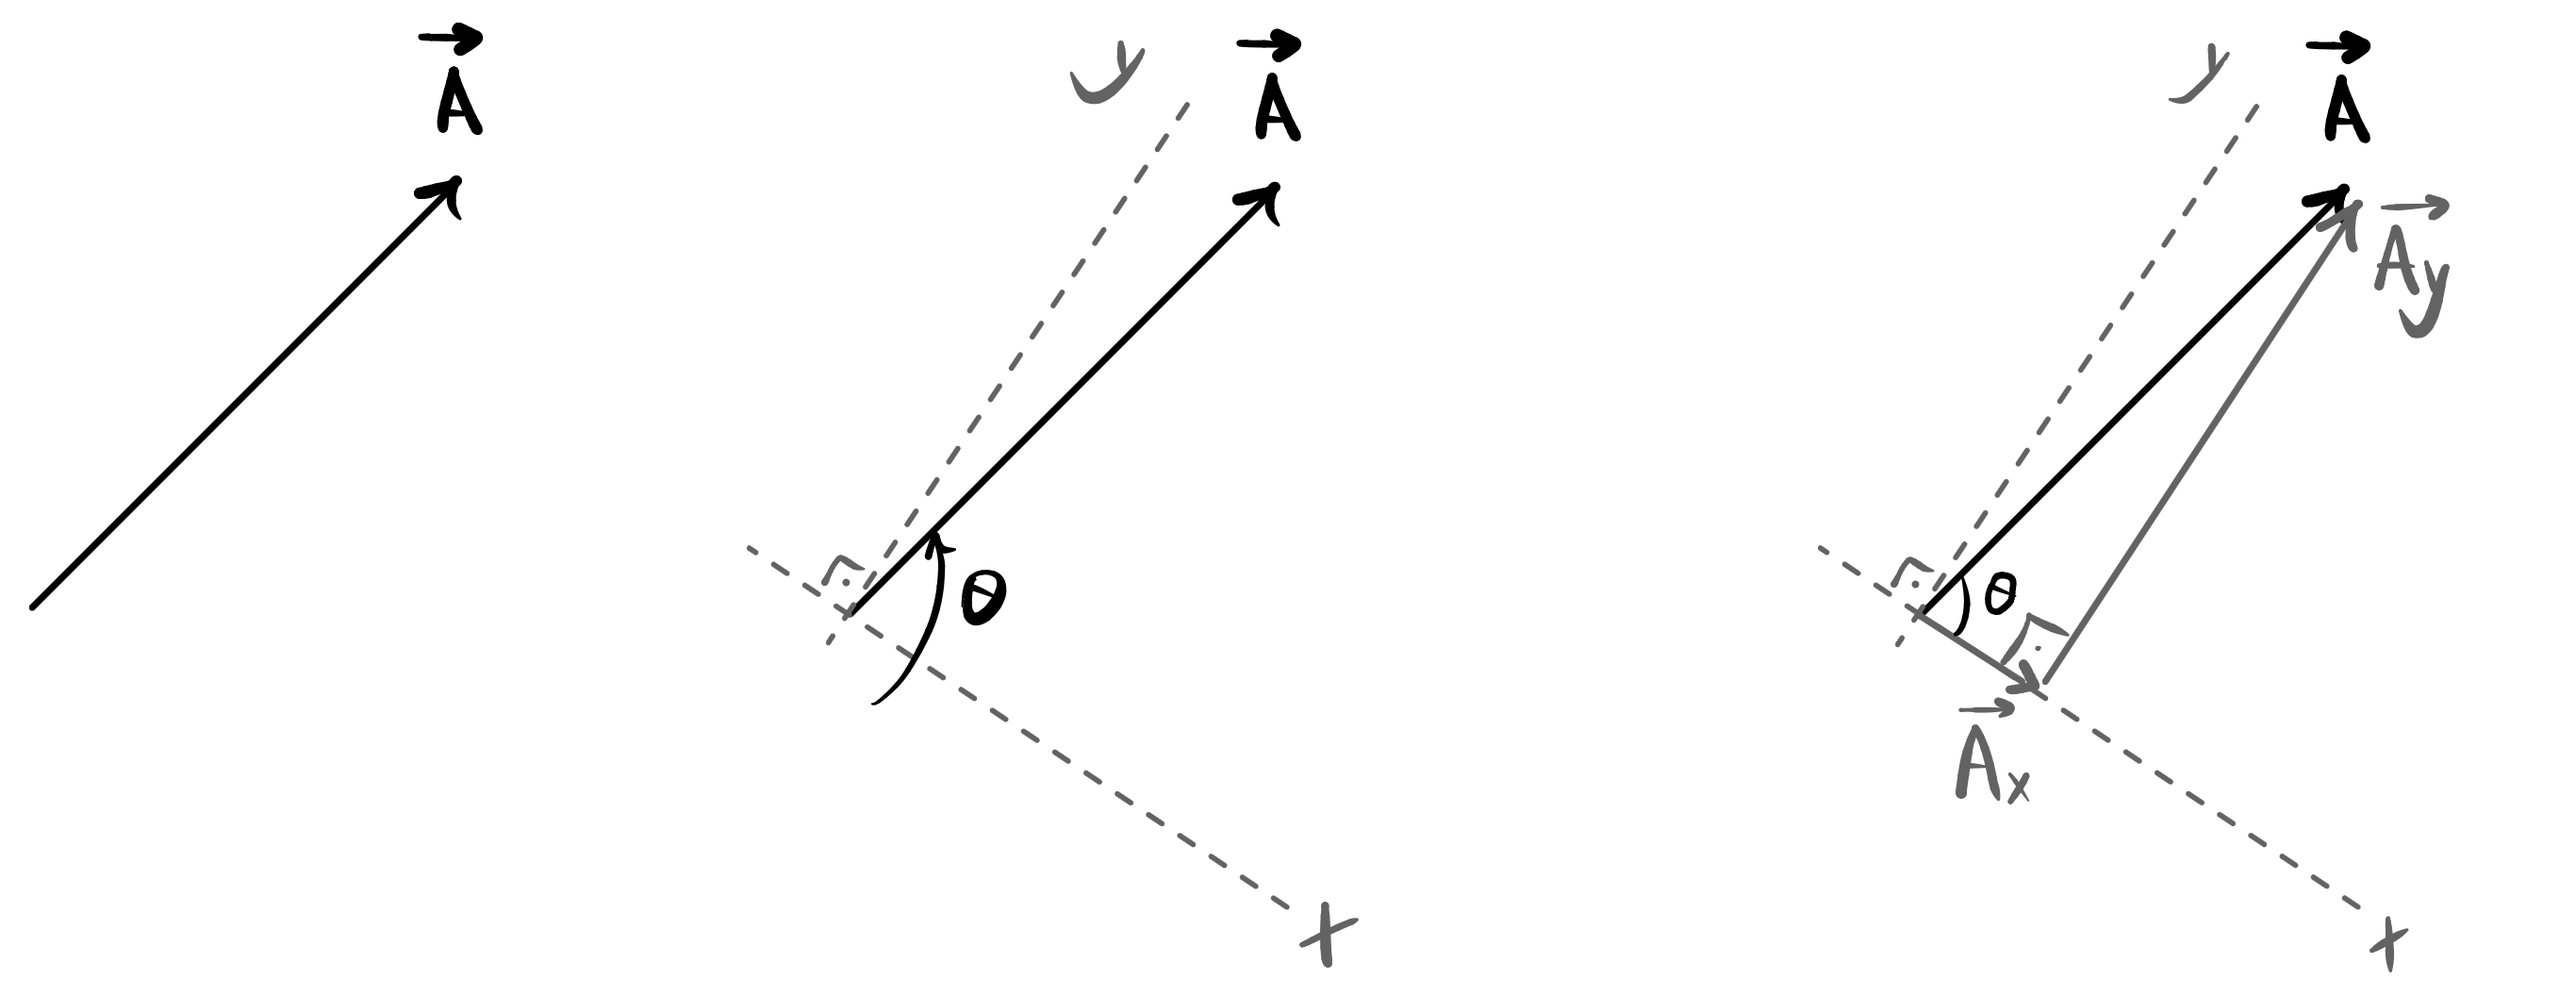
\includegraphics[scale=0.13]{imagenscinematicavetorial/decomporvetores2.jpeg}
    \caption{A decomposição vetorial nas direções perpendiculares quaisquer.}
    \label{fig_cinvet_decomporvetores2}
\end{figure}


Poderíamos ter escolhido quaisquer outras direções nas quais quiséssemos decompor o vetor inicial $\vec{A}.$ Tais direções sequer precisariam ser perpendiculares entre si -- mas nos ateremos sempre a estes casos, dadas as vantagens anteriormente mencionadas. Considere, por exemplo, a Figura \ref{fig_cinvet_decomporvetores2}, que contém o mesmo vetor $\vec{A}$, porém agora as direções perpendiculares $x$ e $y$ nas quais se pretende decompô-lo são outras. Note que o procedimento é exatamente o mesmo: ao projetar o vetor $\vec{A}$ em cada uma dessas direções teremos as suas componentes, o que aparece representado na terceira imagem da figura. Perceba que as mesmas relações de antes são válidas, isto é:

\begin{enumerate}
    \item [(i)] Os vetores $\vec{A}_x$ e $\vec{A}_y$, somados, resultam no vetor $\vec{A};$ ou seja, vale a equação vetorial:

    $$ \vec{A} = \vec{A}_x + \vec{A}_y. $$

    \item [(ii)] Os módulos das componentes $A_x$ e $A_y$ se relacionam com o módulo $A$ do vetor inicial pelo Teorema de Pitágoras \footnote{Isso sempre ocorrerá quando as direções $x$ e $y$ de decomposição forem perpendiculares, porque isso sempre fará com que o triângulo de vetores da terceira imagem das Figuras \ref{fig_cinvet_decomporvetores1} e \ref{fig_cinvet_decomporvetores2} seja um triângulo retângulo.}, de modo que vale a equação algébrica:

    $$ A^2 = A_x^2 + A_y^2.$$

    \item [(iii)] Os módulos das componentes $A_x$ e $A_y$ se relacionam com o módulo $A$ do vetor inicial e com o ângulo $\theta$ que ele faz com a direção $x$ por meio das equações

    $$ \boxed{A_y = A \sin \theta} \quad  \text{ e } \quad \boxed{A_x = A \cos \theta,}$$

    \noindent o que mudou, neste caso, foi apenas as direções de decomposição -- ou seja, o valor de $\theta$ -- de modo que as componentes nas novas direções $x$ e $y$ terão, naturalmente, valores distintos.
\end{enumerate}


\begin{figure}[h]
    \centering
    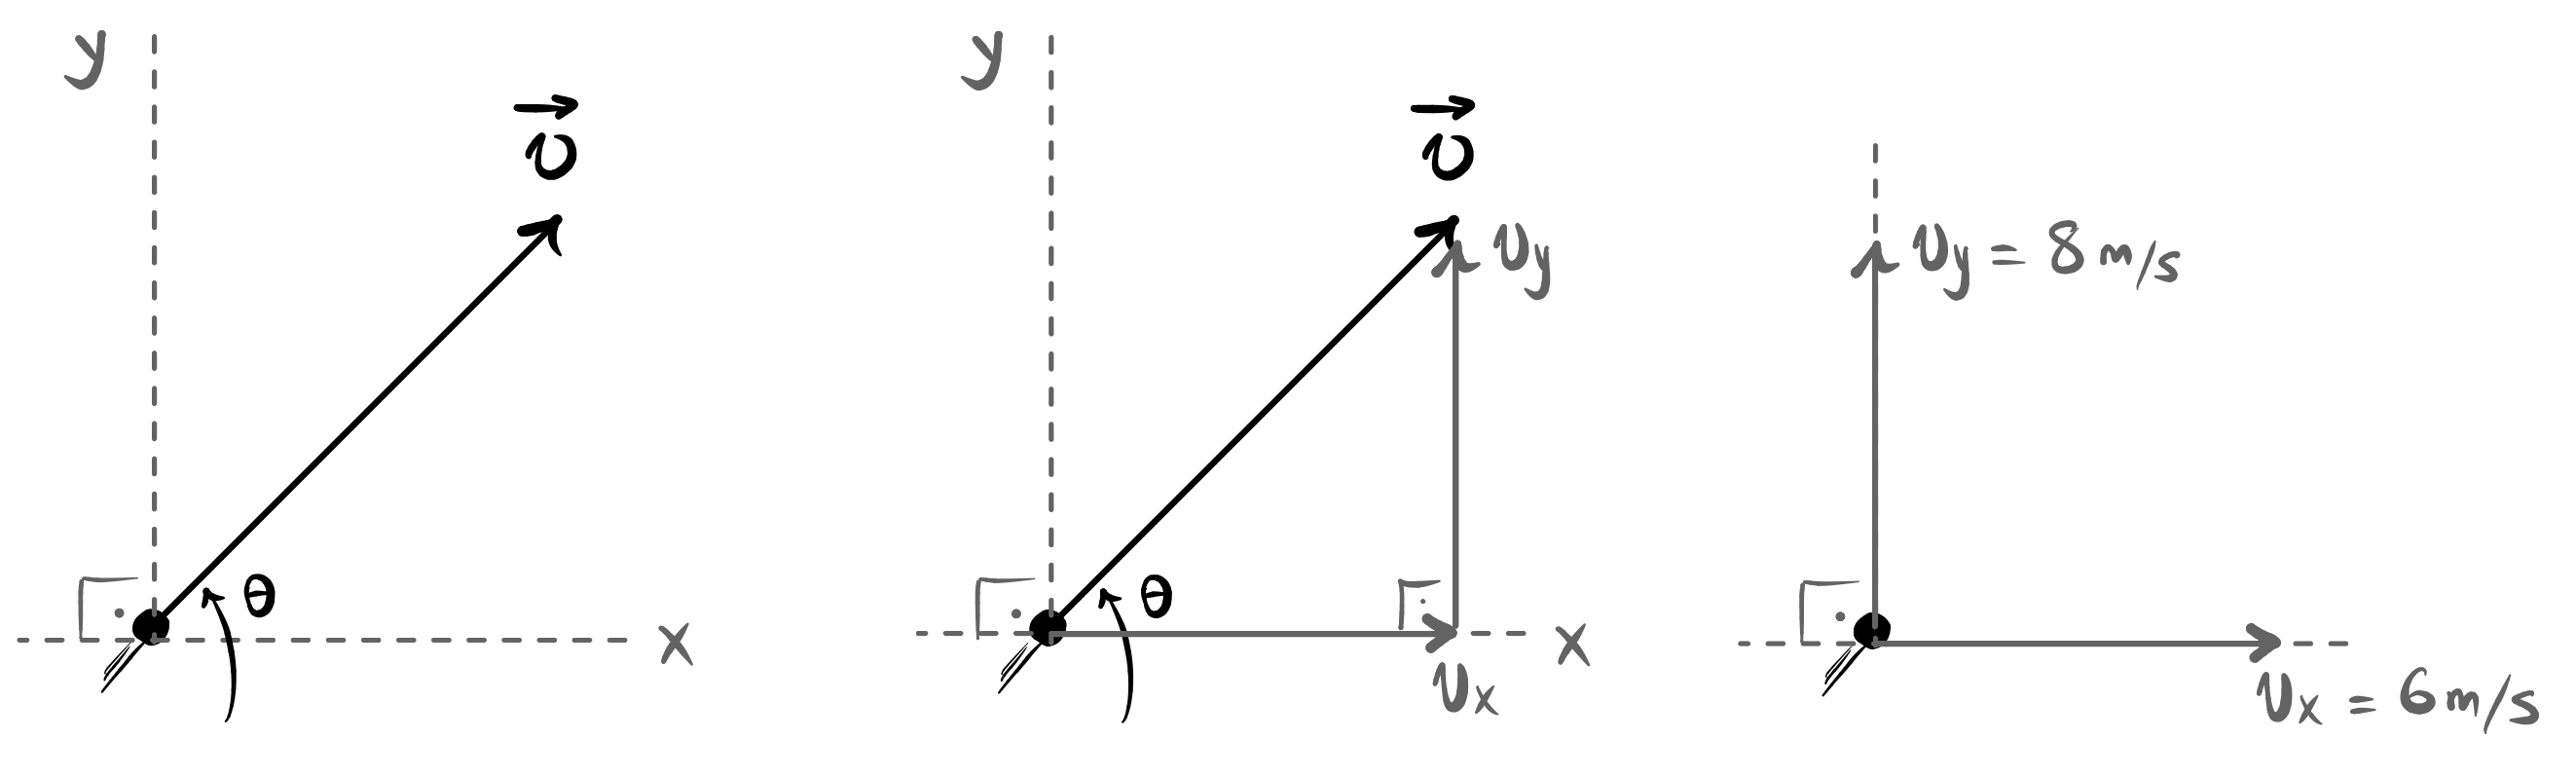
\includegraphics[scale=0.15]{imagenscinematicavetorial/decomporvetores3.jpeg}
    \caption{Fazendo uma decomposição vetorial.}
    \label{fig_cinvet_decomporvetores3}
\end{figure}


Para não deixar totalmente abstrata essa nova operação, avaliemos o caso da Figura \ref{fig_cinvet_decomporvetores3}, em que o ângulo $\theta$ com a direção $x$ é tal que $\sin \theta = 0.8$ e $\cos \theta = 0.6.$ Considere que trata-se de uma bola, que foi lançada com velocidade $v=10$ m/s, fazendo o ângulo $\theta$ em questão com a direção horizontal.





Podemos decompor tal velocidade nas direções $x$ e $y$, e suas componentes podem ser obtidas por meio das razões trigonométricas no triângulo retângulo da segunda imagem da figura:


\begin{align}
    \sin \theta &= \dfrac{v_y}{v} \implies v_y = v \sin \theta = 10 \cdot 0.8 \implies  \boxed{v_y=8 \text{ m/s,}} \nonumber \\
     \cos \theta &= \dfrac{v_x}{v} \implies v_x = v \cos \theta = 10 \cdot 0.6 \implies  \boxed{v_x=6 \text{ m/s.}} \nonumber
\end{align}

Perceba que $v_x^2+v_y^2=6^2+8^2=100=10^2=v^2,$ isto é, os módulos das componentes de velocidade se relacionam com o módulo da velocidade original por meio do Teorema de Pitágoras.

Logo, como os vetores $\vec{v}_x$ e $\vec{v}_y$ somados resultam no vetor inicial $\vec{v},$ em certa medida, lançar uma bola com velocidade $v=10$ m/s em uma direção que faz o ângulo $\theta$ em questão com a horizontal é o mesmo que lançá-la para cima com uma velocidade $v_y=8$ m/s e empurrá-la, ao mesmo tempo, para a direita, fornecendo-a uma velocidade horizontal $v_x=6$ m/s, como mostra a terceira imagem da Figura \ref{fig_cinvet_decomporvetores3}.

Isso será extremamente importante na Física: interpretar um movimento como sendo composto por dois movimentos independentes em duas direções perpendiculares; ou somar o efeito de dois movimentos em direções perpendiculares para obter o movimento composto.


\newpage




\section{Velocidade Vetorial}



\begin{secnivel}[Velocidade Vetorial Média]{I}{Velocidade Vetorial Média}
  
  \eqLdois{def}{cinvet_eq_velocidadevetorialmedia}{\vec{v}_m := \dfrac{\Delta \vec{r}}{\Delta t}}

\end{secnivel}




\secgfe{De onde vem}

Para acompanharmos um movimento bidimensional é comum adotarmos uma origem e localizarmos a partícula por meio de um vetor posição $\vec{r},$ que vai da origem até à posição atual da partícula. Note que isso é bem razoável: se você está acompanhando um passarinho voando, você o localiza por uma linha imaginária que vai dos seus olhos até o objeto em observação. Nesse sentido, os seus olhos seriam a origem do sistema de referência e essa linha pontilhada representa a direção do vetor posição, que aponta para o objeto observado.

Tal situação está representada na Figura \ref{fig_cinvet_vetorposicao01}, em que vetor posição $\vec{r}_1$ vai dos olhos do observador à partícula observada no instante $t_1,$ e o vetor posição $\vec{r}_2$ vai dos olhos do observador à partícula observada no instante $t_2$. O deslocamento vetorial $\Delta \vec{r}$ é definido, naturalmente, como sendo a variação da posição vetorial, ou seja:

$$ \Delta \vec{r} := \vec{r_2} - \vec{r_1},$$

\noindent e, como vimos, fazer essa subtração vetorial é somar o vetor $\vec{r}_2$ com o inverso do vetor $\vec{r}_1,$ o que aparece na segunda e terceira imagem da Figura \ref{fig_cinvet_vetorposicao01}, fornecendo o vetor deslocamento $\Delta \vec{r}$ como sendo o vetor que vai da posição inicial até a posição final.


\begin{figure}[h]
    \centering
    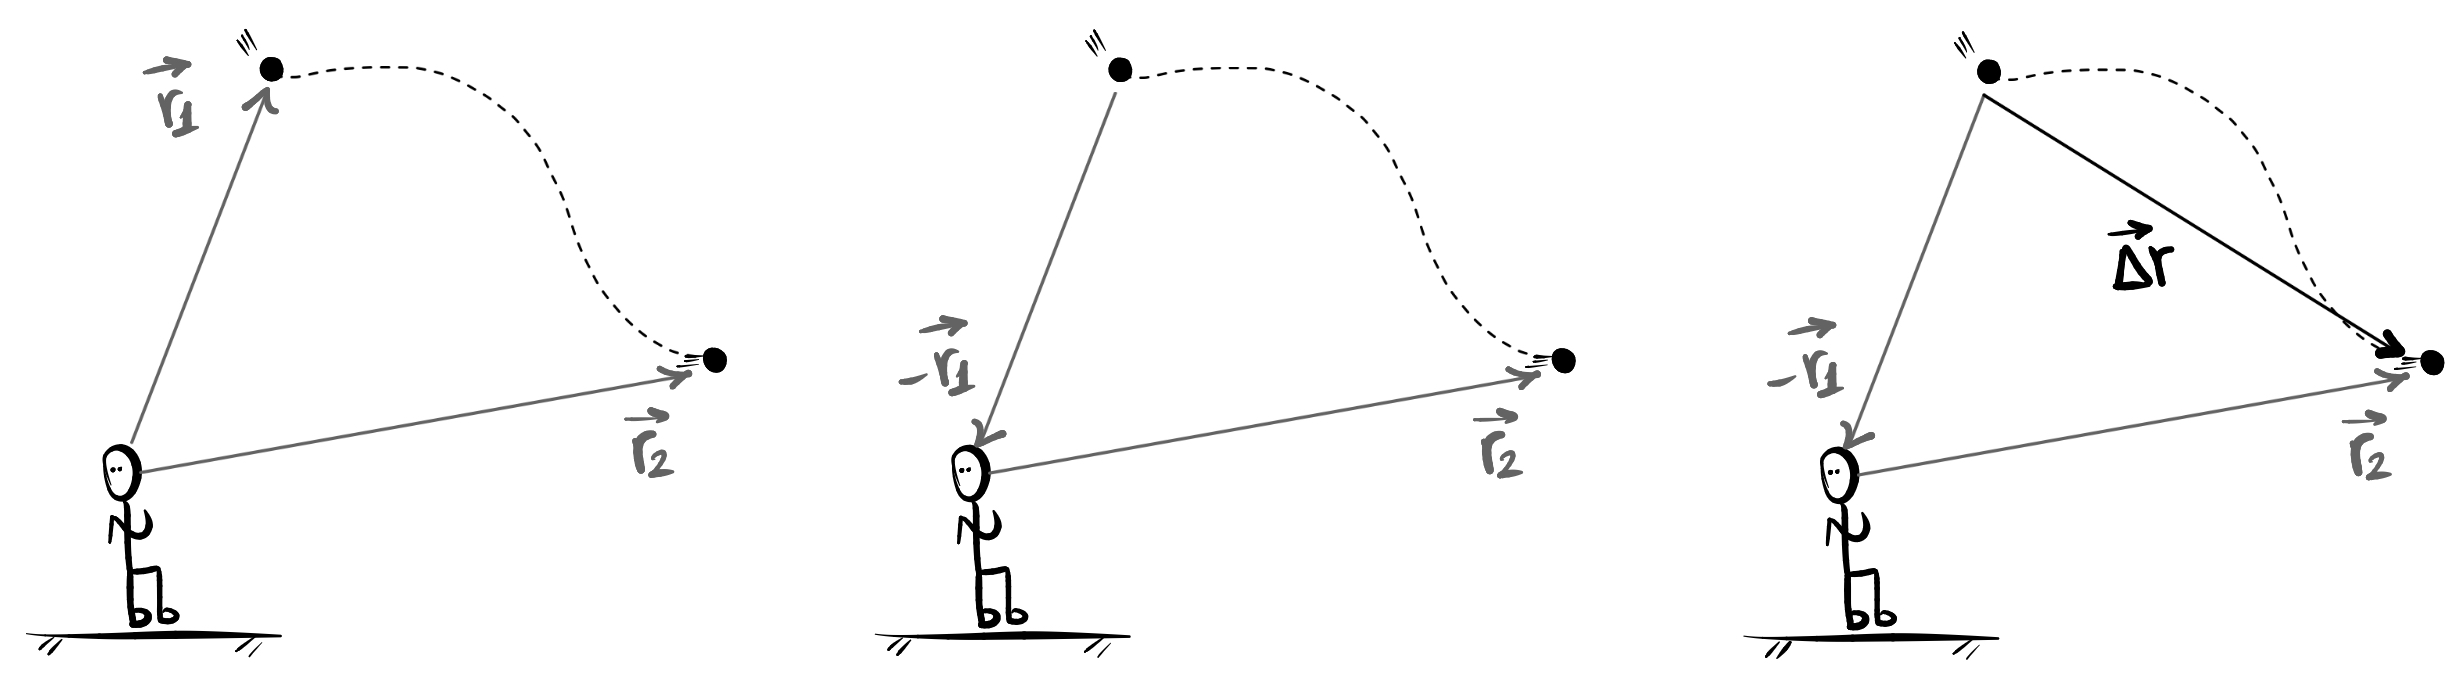
\includegraphics[scale=0.18]{imagenscinematicavetorial/vetorposicao.jpeg}
    \caption{O vetor posição $\vec{r}$ e o deslocamento vetorial $\Delta \vec{r}.$}
    \label{fig_cinvet_vetorposicao01}
\end{figure}

Vale notar que, apesar dos vetores posição $\vec{r}_1$ e $\vec{r}_2$ serem diferentes para diferentes observadores -- ou seja, a posição de um certo objeto no tempo depende do referencial --, o vetor deslocamento é algo absoluto, que não depende do referencial. Isso pode ser notado pela Figura \ref{fig_cinvet_vetorposicao02}, que mostra o mesmo movimento sendo analisado por um observador distinto. Note que os vetores posição $\vec{r}_1$ e $\vec{r}_2$ são diferentes daqueles do referencial da Figura \ref{fig_cinvet_vetorposicao01}; já o vetor deslocamento $\Delta \vec{r}$ é exatamente o mesmo: ele vai da posição inicial até a posição final do objeto.\footnote{O vetor deslocamento será sempre o mesmo para observadores em repouso, naturalmente. Um observador em movimento perceberia um deslocamento distinto.}


\begin{figure}[h]
    \centering
    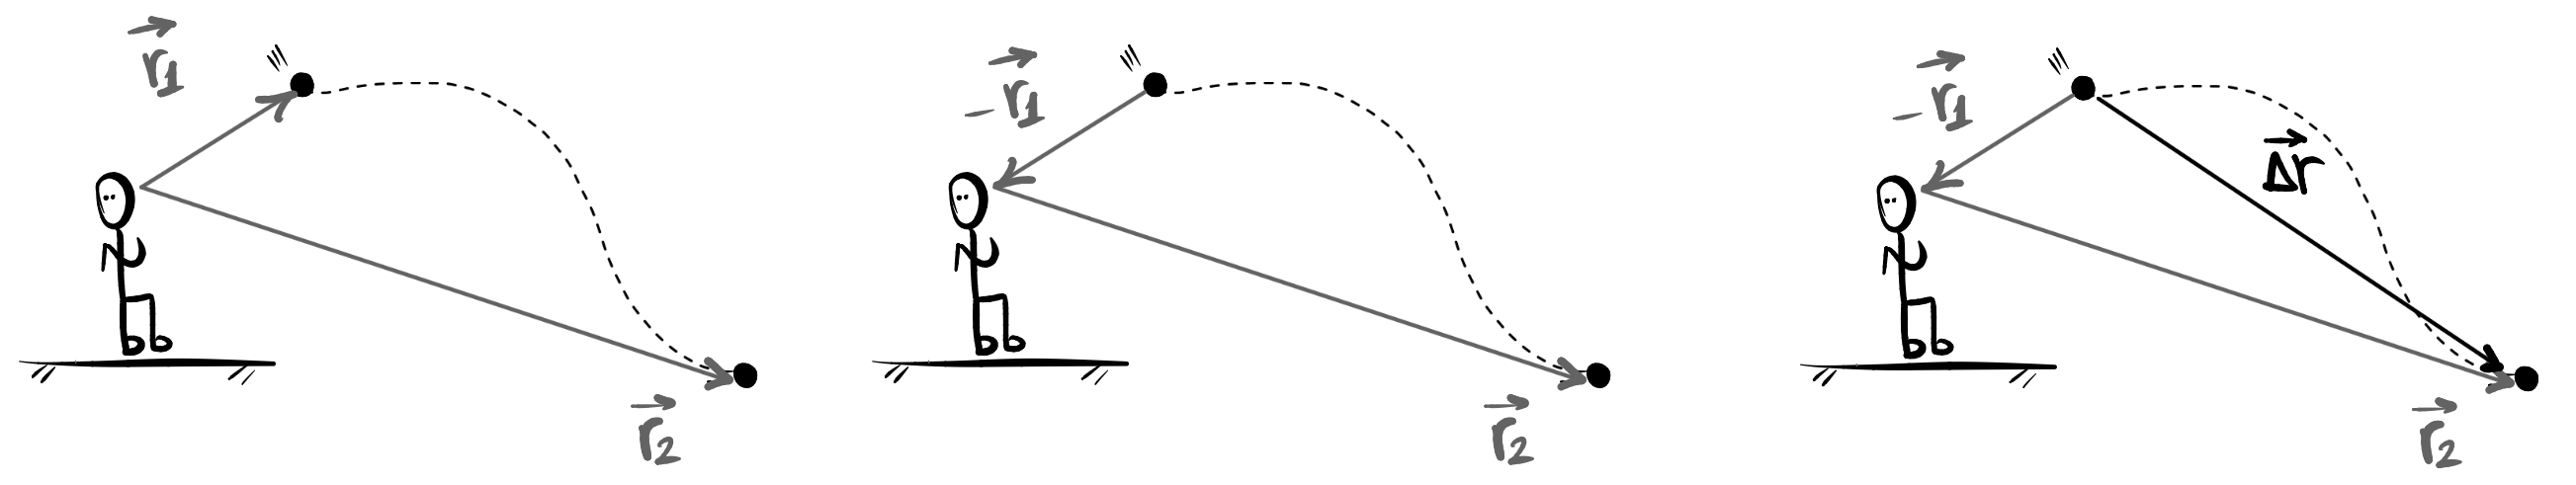
\includegraphics[scale=0.18]{imagenscinematicavetorial/vetorposicao02.jpeg}
    \caption{O vetor deslocamento $\Delta \vec{r}$ visto por um outro referencial em repouso.}
    \label{fig_cinvet_vetorposicao02}
\end{figure}


A Figura \ref{fig_cinvet_deslocamentoedistancia} dá um destaque para o deslocamento do corpo e a sua trajetória, removendo os observadores e os vetores posição, haja vista que o deslocamento e distância são os mesmos, independente do sistema de referência -- desde que ele esteja em repouso. Vale destacar, novamente, a diferença entre as duas grandezas: a distância percorrida mede o comprimento da trajetória do corpo, enquanto o deslocamento mede a distância entre suas posições inicial e final. É importante perceber essa diferença porque, como veremos, existirá uma situação muito importante na qual as duas grandezas irão coincidir -- e essa é a grande razão de definirmos a velocidade vetorial média como o fizemos.



\begin{figure}[h]
    \centering
    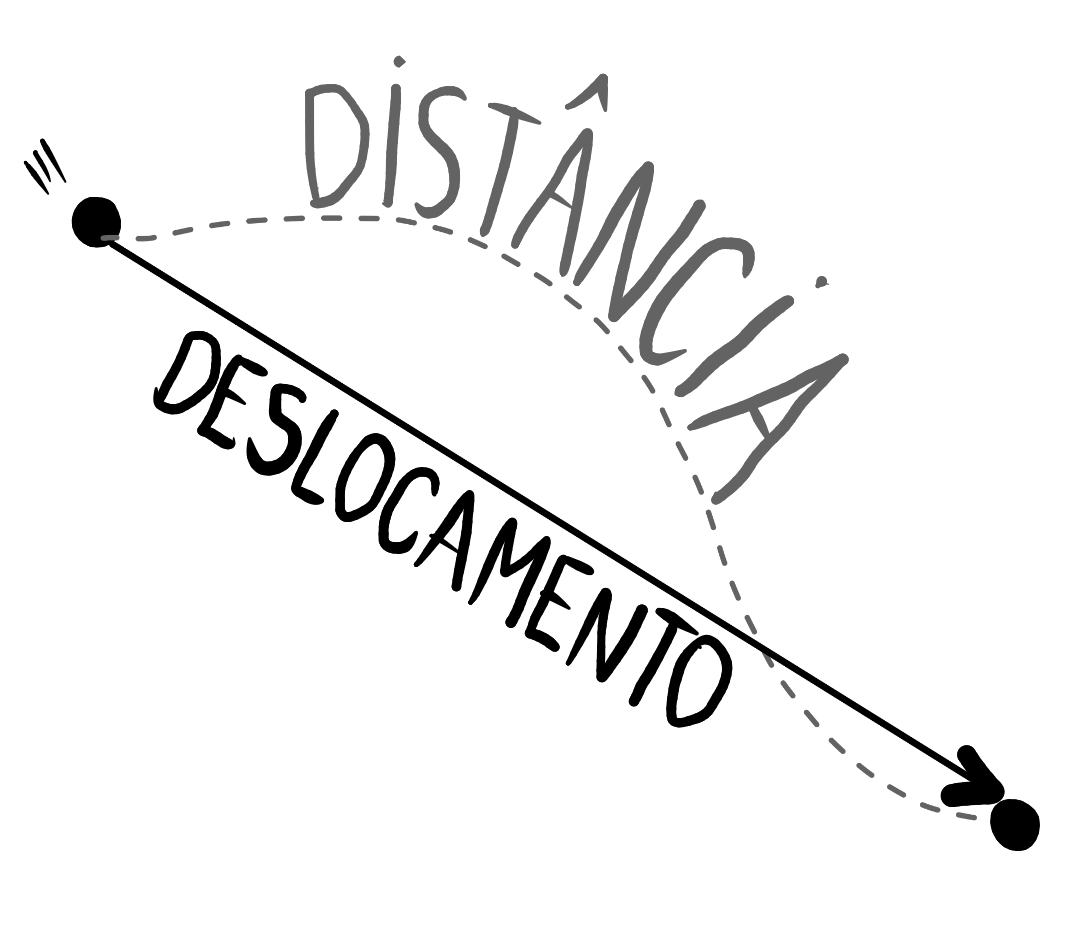
\includegraphics[scale=0.12]{imagenscinematicavetorial/vetordeslocamentoedistancia.jpeg}
    \caption{O vetor deslocamento $\Delta \vec{r}$ e a distância percorrida.}
    \label{fig_cinvet_deslocamentoedistancia}
\end{figure}

Feita essa digressão, definimos a velocidade vetorial média $\vec{v}_m$ como sendo a razão entre o deslocamento vetorial e o intervalo de tempo no qual ele se deu, ou seja:

 $$ \vec{v}_m :=\dfrac{\Delta \vec{r}}{\Delta t}.$$

 Perceba que tal definição é razoável, e não é lá tão diferente de como definimos a velocidade escalar média pela Equação \eqref{mecanica_eq_velocidademedia}, exceto pelo fato de que, aqui, incorporamos na equação o caráter vetorial da velocidade, o que nos possibilitará descrever movimentos em mais de uma dimensão, como havíamos discutido. A Figura \ref{fig_mec_deslocamento_vs_distancia02cinv} ilustra um movimento desse tipo, destacando a diferença entre a distância percorrida e o deslocamento vetorial. Vale ressaltar que, em movimentos nos quais o corpo retorna à posição de origem, o deslocamento vetorial é nulo ainda que a distância percorrida não o seja.

 \begin{figure}[h]
    \centering
    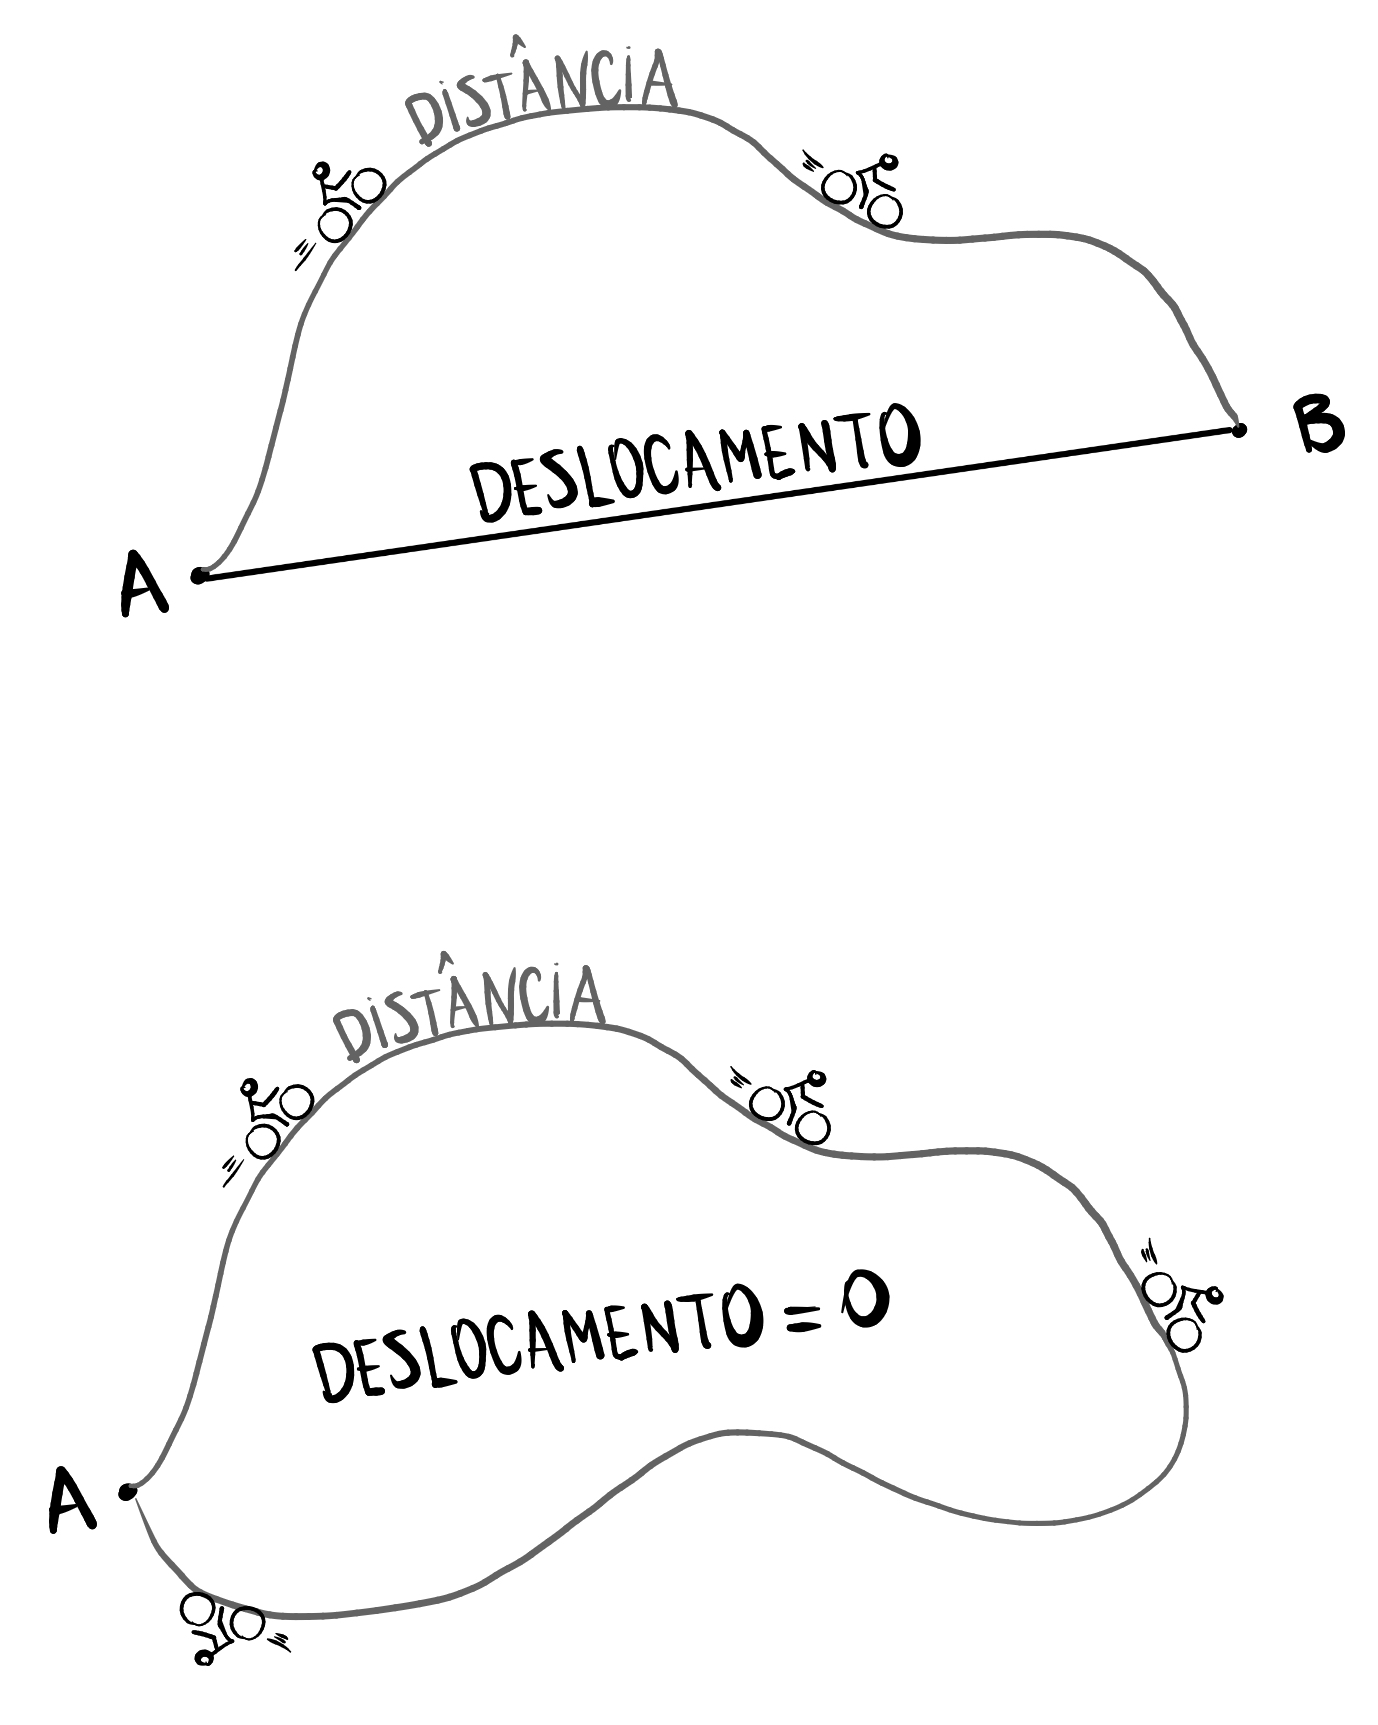
\includegraphics[scale=0.13]{imagensmecanica/deslocamentovsdistancia02.jpeg}
    \caption{A diferença entre o deslocamento $|\Delta \vec{r}|$ e a distância percorrida $d$.}
    \label{fig_mec_deslocamento_vs_distancia02cinv}
\end{figure}


Pela definição feita, o vetor velocidade média $\vec{v}_m$ é basicamente o vetor deslocamento $\Delta \vec{r}$ multiplicado por um escalar, isto é, o número real $\sfrac{1}{\Delta t}$. E, como o intervalo de tempo é sempre positivo, tal número será sempre positivo, de modo que o vetor $\vec{v}_m$, sendo um múltiplo positivo do vetor $\Delta \vec{r}$, apontará sempre na mesma direção e sentido deste. Logo, para uma partícula em movimento, seu vetor velocidade média sempre apontará na direção que une a posição inicial à posição final, apontando no sentido da posição inicial para a posição final.
 

 

\secgfe{Onde é usada}

A verdade é que é bastante raro usarmos diretamente a Equação \eqref{cinvet_eq_velocidadevetorialmedia}. Faremos, em breve, alguns exemplos, de modo que ficará claro para o leitor como ele pode precisar usar tal equação em certos problemas. Contudo, já adianto que tais exemplos são um pouco artificiais e é pouco provável que o leitor precise fazer cálculos como estes em algum momento.

Dito isso, por qual razão, então, estudamos tal equação? Como veremos em breve, o mais importante não é a fórmula e o uso dela em si, mas sim uma consequência que está contida, implicitamente, dentro dela. Tal consequência é tão importante que dedicaremos um espaço exclusivo para ela, nas \textbf{observações} sobre essa equação.




\secgfe{Erros comuns}

Novamente, o erro mais comum aqui é confundir distância com deslocamento. Note que, na Equação \eqref{cinvet_eq_velocidadevetorialmedia}, o que entra no numerador é o deslocamento, e não a distância percorrida.



\secgfe{Observações}


Como levantado anteriormente, existe uma consequência importante, que diz algo extremamente relevante a respeito da velocidade de um corpo, e está contida na forma como definimos a Equação \eqref{cinvet_eq_velocidadevetorialmedia}. Note que tal equação define o vetor \textbf{velocidade média $\vec{v}_m$} de um corpo entre dois instantes, digamos $t_1$ e $t_2$. Veja o que acontece quando fazemos o instante $t_2$ ser muito próximo do instante $t_1$, ou seja, o intervalo $\Delta t$ em que analisamos o movimento passa a ser cada vez mais curto. 



\begin{figure}[h]
    \centering
    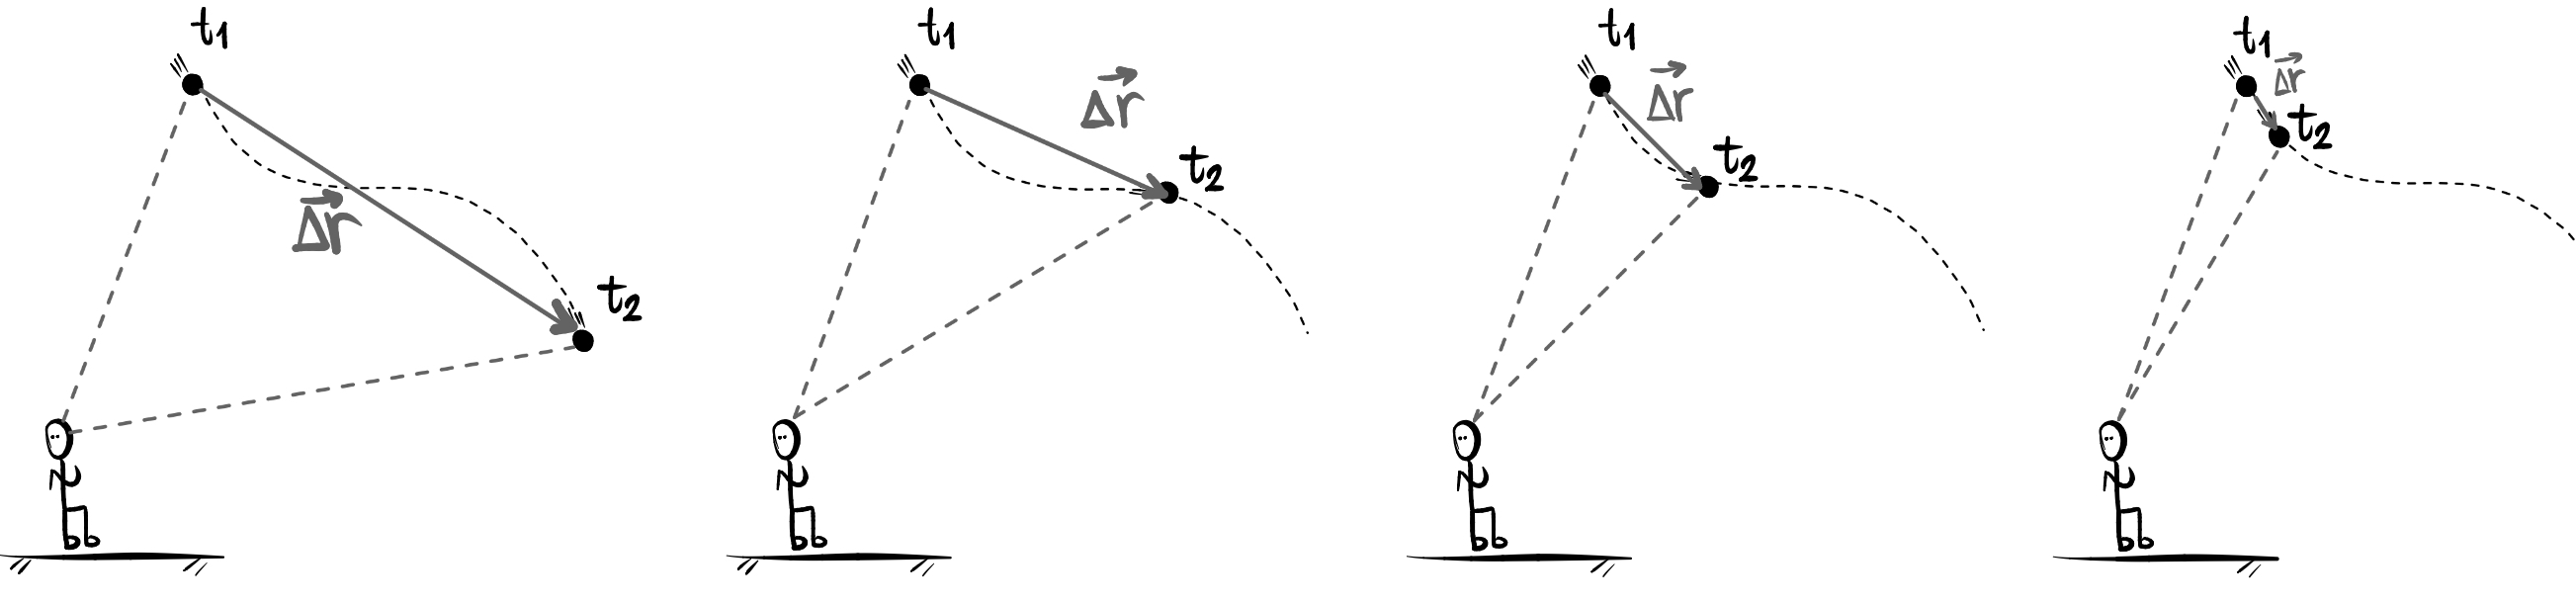
\includegraphics[scale=0.20]{imagenscinematicavetorial/deltatpequeno.jpeg}
    \caption{O vetor deslocamento $\Delta \vec{r}$ avaliado em um intervalo de tempo cada vez menor.}
    \label{fig_cinvet_deltatpequeno}
\end{figure}

Isso aparece na Figura \ref{fig_cinvet_deltatpequeno}, em que estudamos o mesmo movimento, porém analisado em um intervalo de tempo cada vez mais curto. As linhas pontilhadas saindo dos olhos do observador representariam as direções dos vetores posição inicial e final -- o que sequer é relevante, haja vista que o deslocamento sempre apontará da posição inicial do objeto para a sua posição final, mas preferimos deixar tais segmentos de marcação.

Digamos, para fins didáticos, que o intervalo de tempo inicial é $\Delta t = t_2-t_1 = 1 $s. Na segunda imagem da figura, digamos que reduzimos tal intervalo para $\Delta t = t_2-t_1 = 0.1 $s, e na terceira imagem, para $\Delta t = t_2-t_1 = 0.01 $s. Na quarta imagem, digamos que o intervalo de tempo analisado foi de um milésimo de segundo, ou seja, $\Delta t = t_2-t_1 = 0.001 $s.






Perceba que, à medida que o intervalo de tempo fica cada vez mais curto\footnote{Neste caso, o intervalo $\Delta t = t_2-t_1$ está diminuindo porque estamos fazendo $t_2$ se tornar cada vez mais próximo de $t_1.$ O instante $t_1,$ por sua vez, está sendo considerado fixo.}, duas coisas importantes acontecem:

\begin{enumerate}
    \item [(i)] A velocidade média calculada entre os instantes $t_1$ e $t_2$ fica cada vez mais próxima da velocidade instantânea da partícula no instante $t_1,$ isto é, sua velocidade exata em $t_1$, uma vez que a média é feita em um intervalo de tempo tão curto que praticamente não dá tempo de a velocidade variar substancialmente.
    
    \item [(ii)] Quando o intervalo de tempo fica realmente muito pequeno, como é o caso de avaliar para um milésimo de segundo, na última imagem da Figura \ref{fig_cinvet_deltatpequeno}, o módulo do vetor deslocamento $\Delta \vec{r}$ coincide com a distância percorrida $d$ e se torna \textbf{tangente à trajetória.} Este fato é tão importante que merece uma atenção própria: a Figura \ref{fig_cinvet_deslocamentoedistanciazoom} mostra um zoom na situação do intervalo de tempo de um milésimo de segundo -- a última situação da Figura \ref{fig_cinvet_deltatpequeno}. \\


\begin{figure}[h]
    \centering
    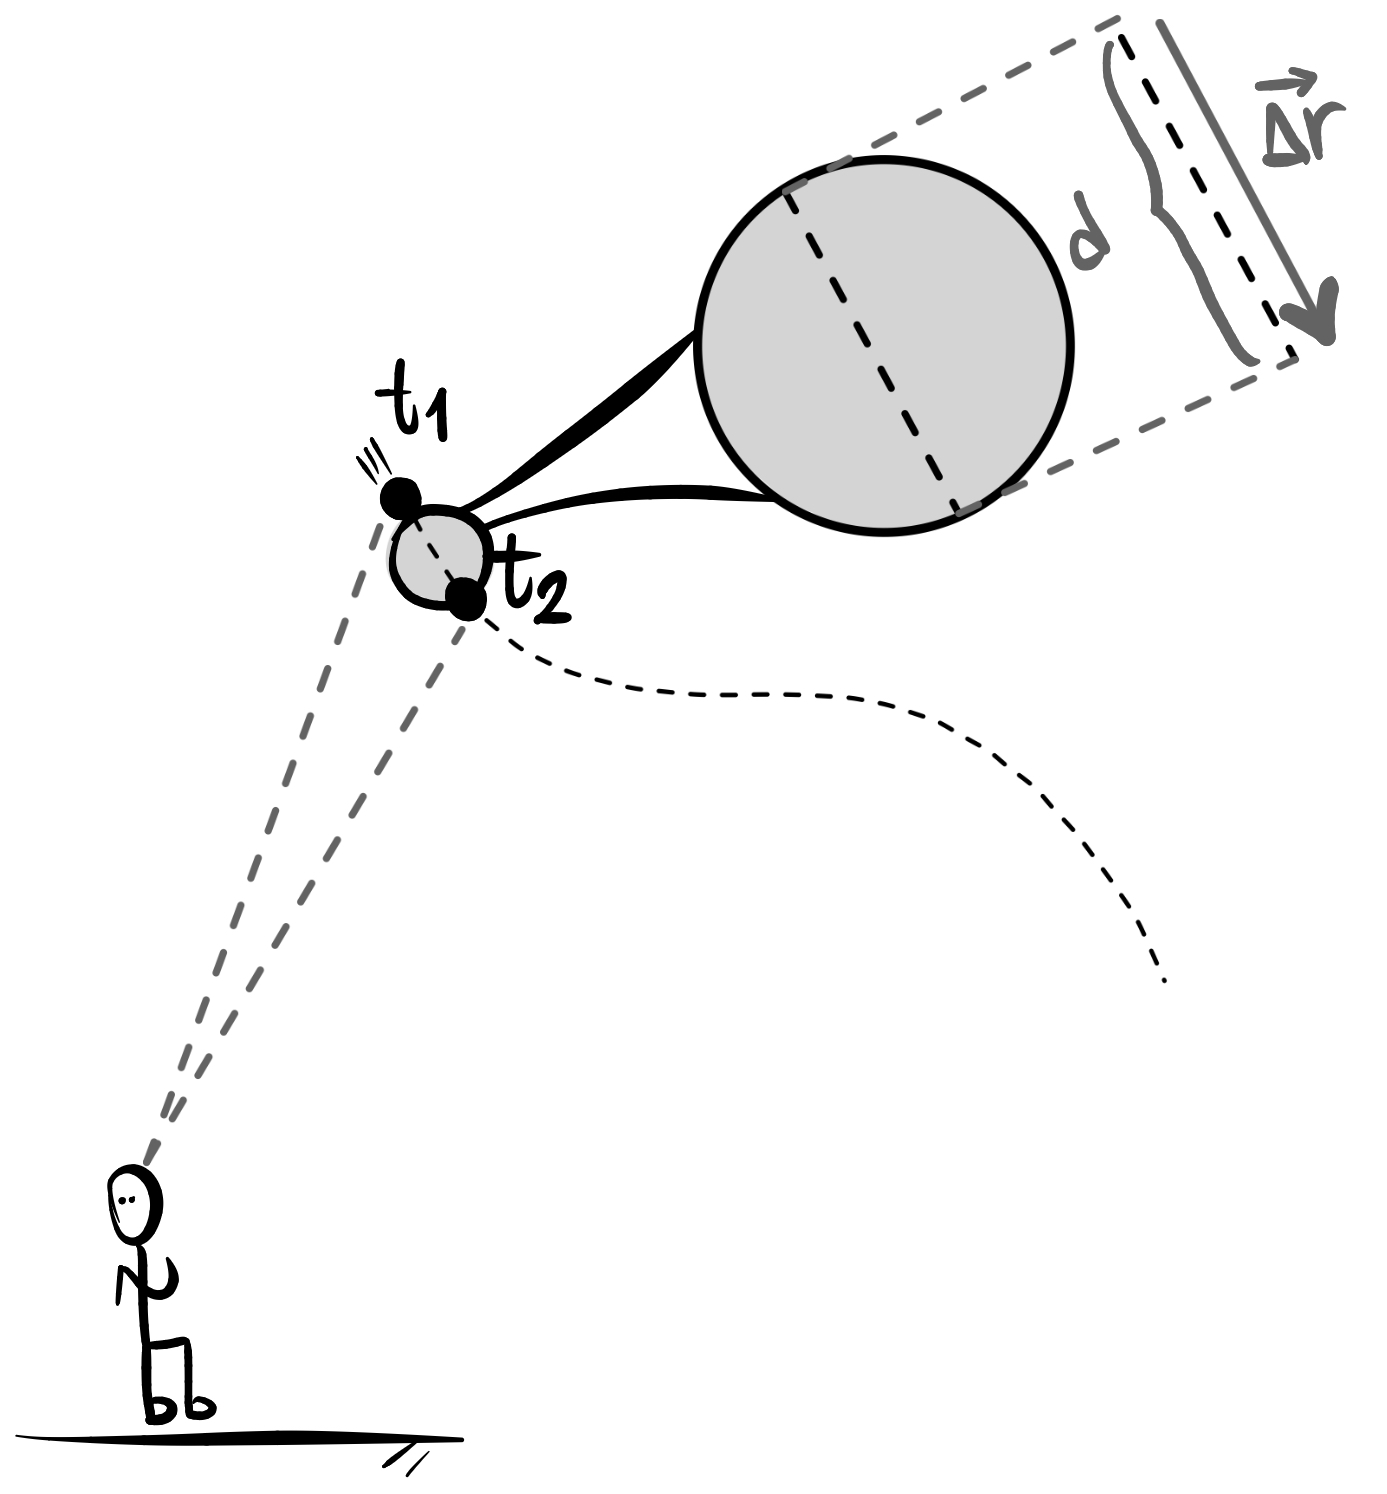
\includegraphics[scale=0.12]{imagenscinematicavetorial/zoomdeltaredistancia.jpeg}
    \caption{O módulo do vetor deslocamento $\Delta \vec{r}$ coincide com a distância percorrida $d$ para intervalos de tempo muito curtos.}
    \label{fig_cinvet_deslocamentoedistanciazoom}
\end{figure}
  
     Perceba que, por mais curvilíneo e esquisito que possa ser um movimento, em um intervalo de tempo suficientemente pequeno, ele se aproxima de uma reta.\footnote{Isso ocorre porque, sendo o tempo suficientemente pequeno -- pense em algo como um milésimo de um centésimo de um bilionésimo de segundo -- praticamente não deu tempo de o corpo se mover, seja para fazer uma curva ou se afastar substancialmente da posição inicial.} Desse modo, o deslocamento vetorial $\Delta \vec{r}$ -- que é a distância em linha reta da posição final à inicial -- coincide com a distância percorrida $d$, e a velocidade vetorial média instantânea $\vec{v}$ tem a direção da tangente à curva naquele ponto, apontando para o sentido do movimento.

     Daqui extraímos a \textbf{conclusão mais importante} de definirmos a velocidade vetorial média da forma como fizemos na Equação \eqref{cinvet_eq_velocidadevetorialmedia}: para uma partícula em um movimento qualquer, a sua velocidade vetorial $\vec{v}$, em cada instante,\footnote{Para que fique absolutamente claro este ponto, estamos falando da velocidade em cada instante porque, se fizermos a velocidade média entre $t_1=2.000$s e $t_2=2.001$s, o leitor há de concordar que tal valor será praticamente igual à velocidade da partícula no instante $t_1=2.000$s, uma vez que passou tão pouco tempo que a mudança na velocidade deve ter sido ínfima.} é tangente à sua trajetória e o seu módulo, naquele instante, coincide com o módulo da velocidade escalar média.

     
     A última parte da conclusão se refere ao fato de que, como distância e deslocamento coincidem, as razões
     
     
     $$ \dfrac{d}{\Delta t} \quad \text{e} \quad \dfrac{|\Delta \vec{r}|}{\Delta t}$$

     \noindent fornecerão exatamente o mesmo valor.
     

    
\end{enumerate}

Como dito, a parte mais importante do estudo da Equação \eqref{cinvet_eq_velocidadevetorialmedia} não é a aplicação da equação em si, mas sim uma informação que está contida implicitamente nela. Tal informação aparece ilustrada na Figura \ref{fig_cinvet_velocidadetangente} -- agora, para qualquer tipo de movimento bidimensional, o leitor já sabe exatamente qual é a propriedade geométrica que a velocidade do corpo em movimento deve satisfazer em todos os instantes: ela é sempre tangente à trajetória, apontando no mesmo sentido em que o movimento se dá.


\begin{figure}[h]
    \centering
    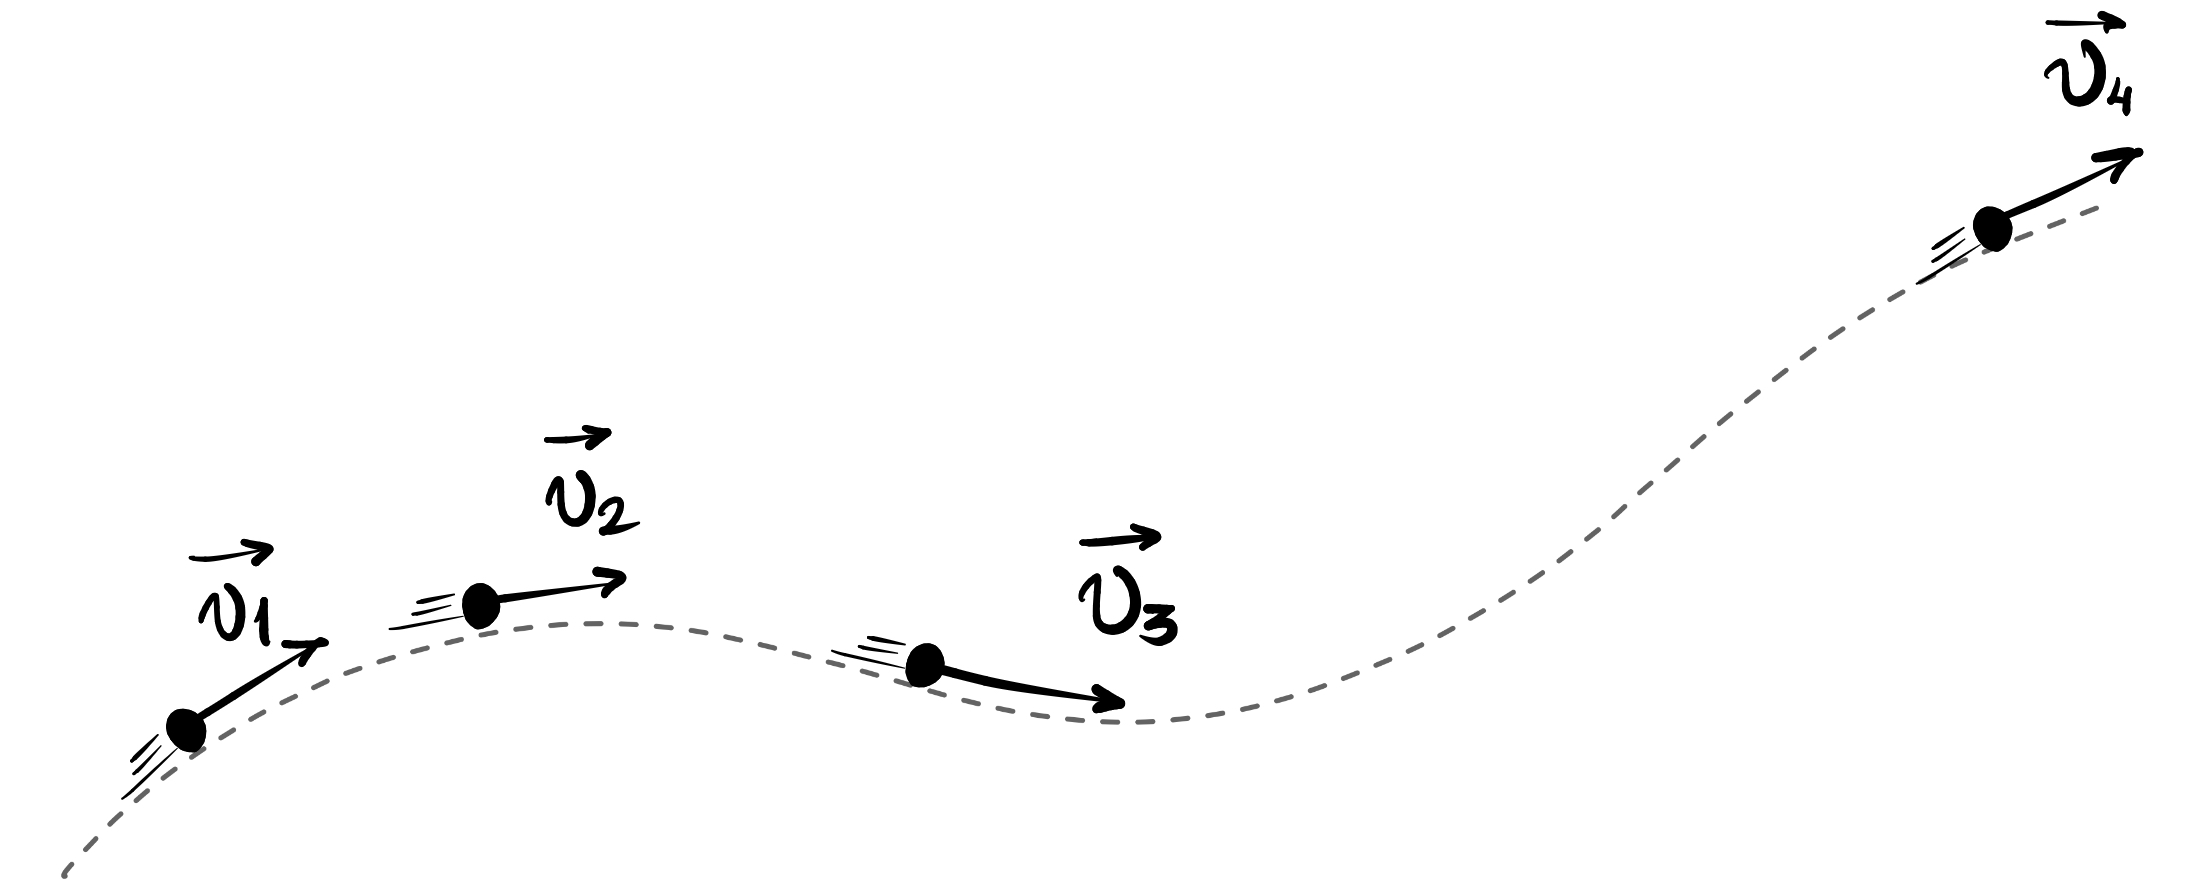
\includegraphics[scale=0.12]{imagenscinematicavetorial/velocidadetangente.jpeg}
    \caption{A velocidade vetorial $\vec{v}$ de uma partícula em movimento é sempre tangente à sua trajetória.}
    \label{fig_cinvet_velocidadetangente}
\end{figure}
  
É deste fato que decorre o fenômeno de \textit{sair pela tangente}. A velocidade aponta na direção e sentido para a qual o movimento tende a acontecer. Desse modo, na ausência de quaisquer forças ou interferências, um corpo sempre irá se mover exatamente na mesma direção e sentido para a qual aponta a sua velocidade. Considere o caso de uma pedra, amarrada por um barbante, que é posto a girar em torno de um centro fixo. Tal situação é a que aparece no primeiro desenho da Figura \ref{fig_cinvet_sairpelatangente}.


\begin{figure}[h]
    \centering
    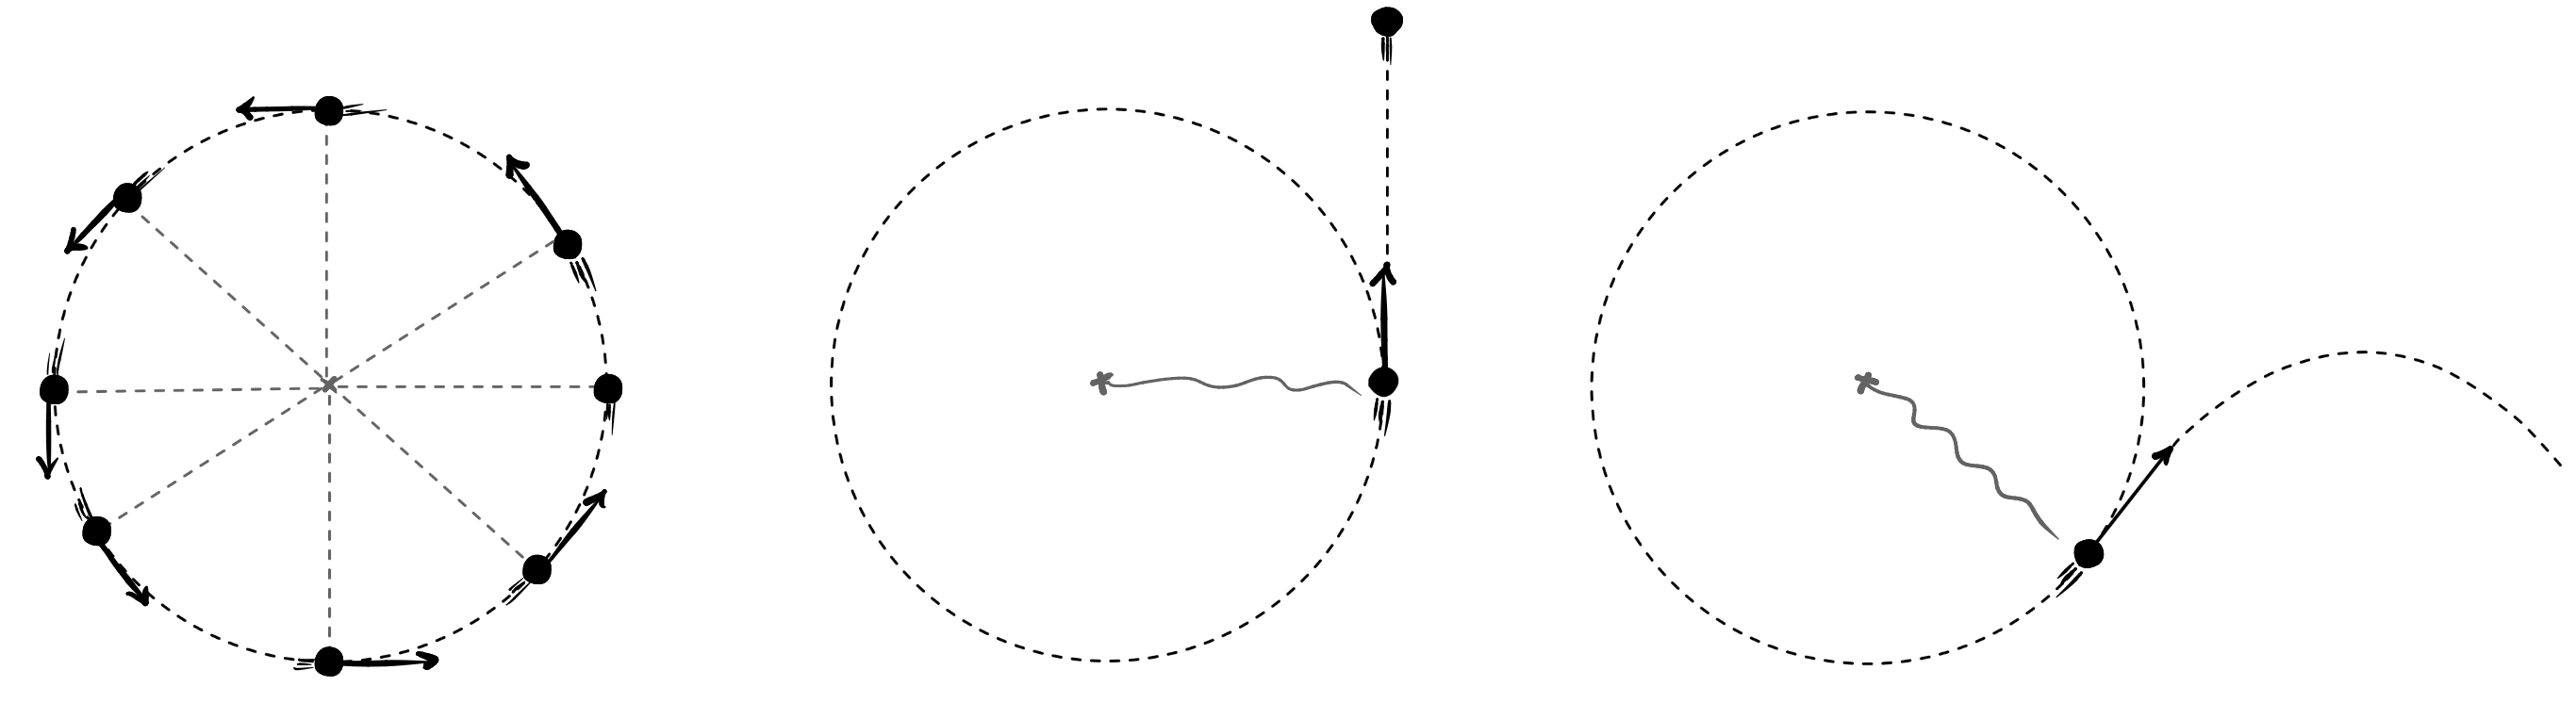
\includegraphics[scale=0.15]{imagenscinematicavetorial/sairpelatangente.jpeg}
    \caption{A velocidade vetorial $\vec{v}$ aponta na direção e sentido para onde o movimento se dá.}
    \label{fig_cinvet_sairpelatangente}
\end{figure}

Como já sabemos, em cada ponto a velocidade será tangente à trajetória. A pedra só não se move diretamente em tal direção porque existe uma força -- associada à sua conexão com o barbante -- que a confina e a obriga a se mover na trajetória circular. Contudo, se em qualquer ponto o barbante se romper, a partícula se moverá exatamente na direção para onde aponta a sua velocidade -- ela sairá na direção da tangente à circunferência, uma vez que a velocidade é tangente à circunferência. Tais situações estão ilustradas nas duas próximas imagens da Figura \ref{fig_cinvet_sairpelatangente}, que considera o barbante se rompendo para a pedra em duas posições diferentes. \footnote{Note que, no terceiro desenho da figura, a bolinha sai exatamente na direção da tangente. Sua trajetória, contudo, não é uma linha reta nessa direção devido à ação da gravidade, que puxa a bolinha para baixo, afetando e alterando a sua trajetória ao longo do movimento.}

\vspace{0.3cm}

%Exemplo resolvido

\begin{exemplo}[Nível I]\label{exemplo_cinematicavetorial_velocidadevetorialex01}

Um objeto sofre os sucessivos deslocamentos representados na Figura \ref{fig_cinvet_velocidadevetorialexemplo01}. Se o movimento todo dura $74$s, encontre seu vetor velocidade média ao longo de todo o intervalo -- ou seja, encontre seu módulo, direção e sentido.\\

Considere $\sin \theta = 0,8$ e $\cos \theta = 0,6.$

{
\centering
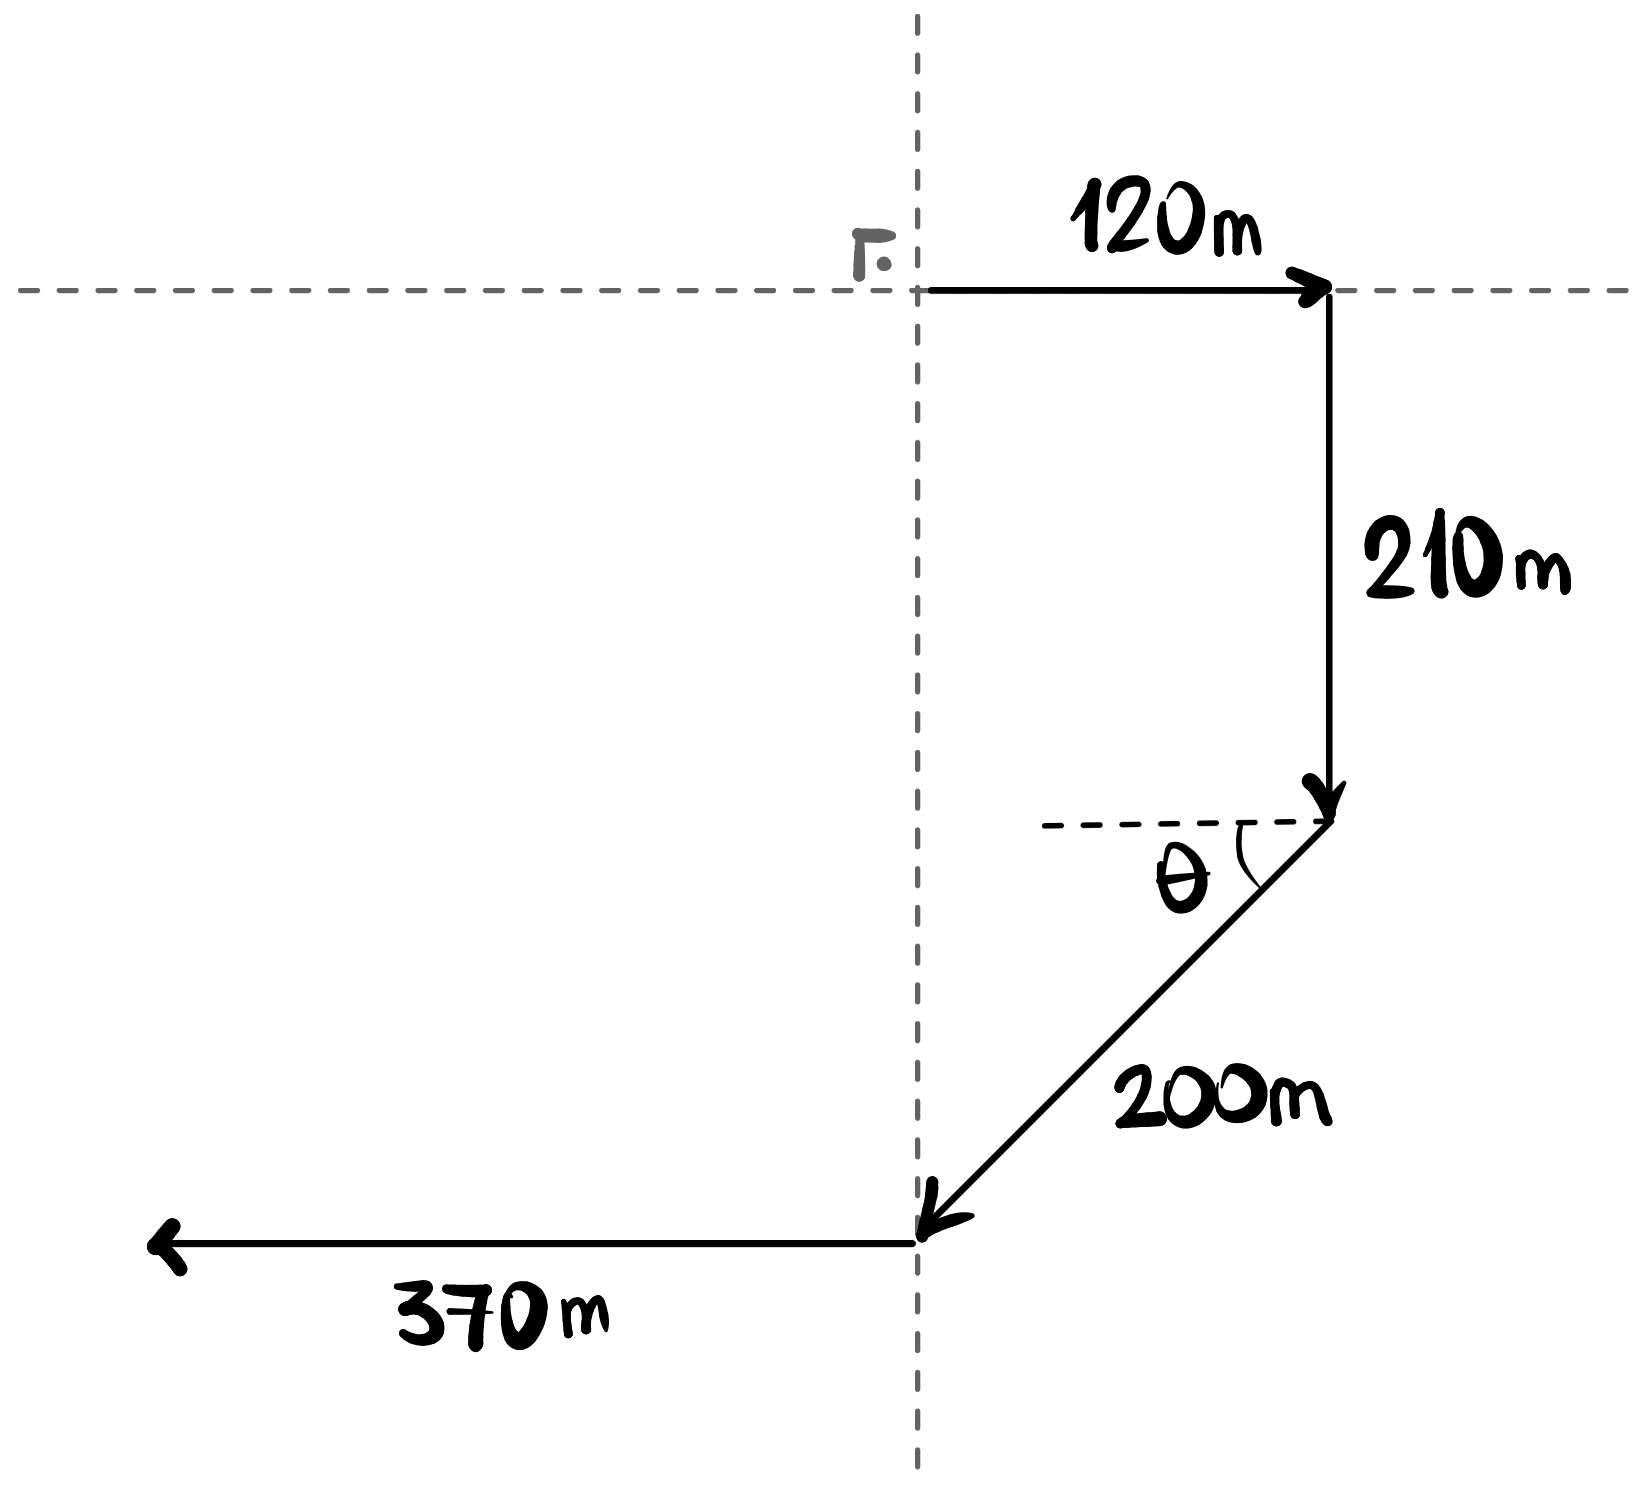
\includegraphics[width=0.3\linewidth]{imagenscinematicavetorial/velocidadevetorialexemplo1.jpeg}
\captionof{figure}{}
\label{fig_cinvet_velocidadevetorialexemplo01}
} 

\resolucao

Como mostra a primeira imagem da Figura \ref{fig_cinvet_velocidadevetorialexemplo0102}, sejam $a$ e $b$ os deslocamentos horizontal e vertical, respectivamente, oriundos do deslocamento inclinado de $200$ m. Podemos obter tais deslocamentos por meio de trigonometria básica:

$$ \sin \theta = \dfrac{b}{200} = 0.8 \implies \boxed{b=160 \text{ m}} \quad \text{e} \quad \cos \theta = \dfrac{a}{200} = 0.6 \implies \boxed{a=120 \text{ m.}}$$


{
\centering
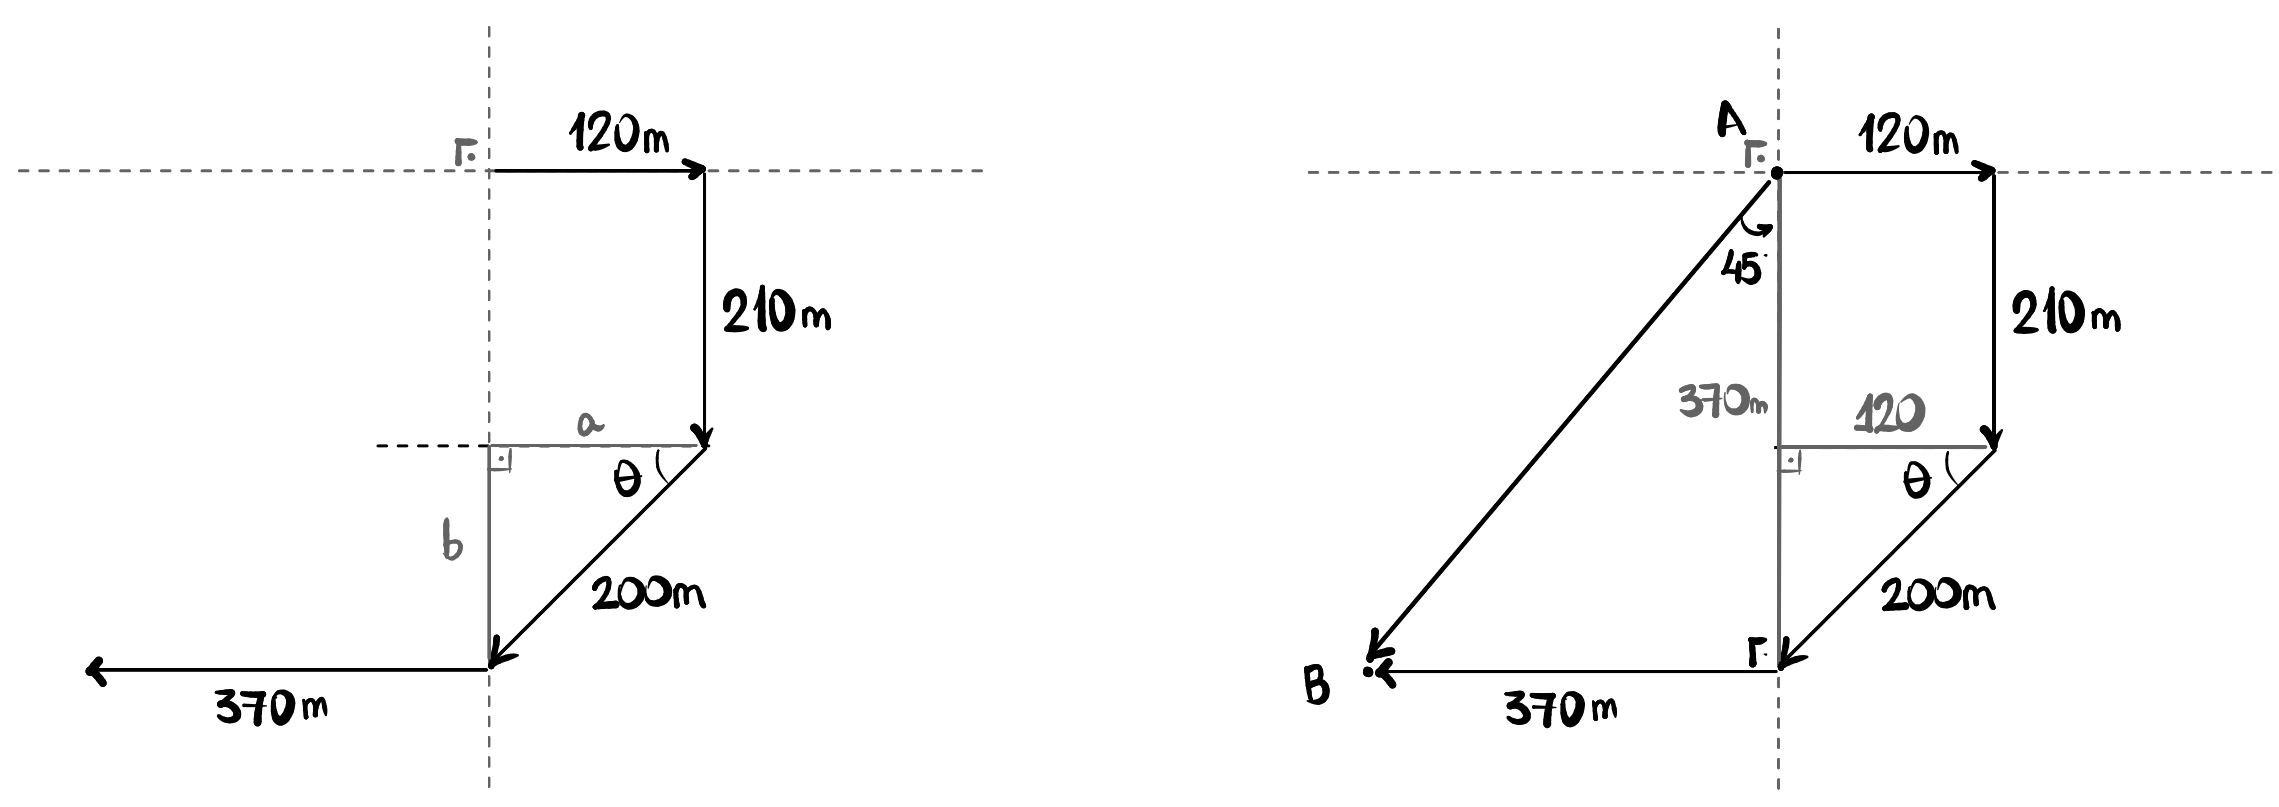
\includegraphics[width=0.8\linewidth]{imagenscinematicavetorial/velocidavetorialexemplo0102.jpeg}
\captionof{figure}{}
\label{fig_cinvet_velocidadevetorialexemplo0102}
} 

Com isso, podemos entender o vetor deslocamento de $200$m inclinado de $\theta$ como sendo composto por um deslocamento horizontal para a esquerda de $120$m --- que faz a partícula retornar ao alinhamento vertical inicial --- seguido de um deslocamento vertical para baixo de $160$m. Logo, o deslocamento vertical total é de $210+160=370$m, o que aparece na segunda imagem da Figura \ref{fig_cinvet_velocidadevetorialexemplo0102}. \\

Assim, o vetor deslocamento total $\Delta \vec{r}$ vai da posição inicial $A$ à posição final $B$, e aparece representado na segunda imagem da figura: pelo Teorema de Pitágoras, vemos que ele terá um módulo dado por $|\Delta \vec{r}|=370 \sqrt{2}$m e fará um ângulo de $45^\circ$, uma vez que o triângulo retângulo tem catetos iguais (a 370m, no caso), de modo que ele é isósceles.

Logo, como o movimento dura $\Delta t = 74$s, o módulo da velocidade vetorial média é

$$ |\vec{v}_m| = \dfrac{|\Delta \vec{r}|}{\Delta t} = \dfrac{370\sqrt2 \text{ m}}{74 \text{ s}} \implies \boxed{|\vec{v}_m| =5\sqrt2 \text{ m/s,}} $$

\noindent e ela aponta, naturalmente, na mesma direção e sentido do vetor $\Delta \vec{r}:$ inclinada de $45^\circ$ no sentido anti-horário em relação à parte inferior do eixo vertical, como mostra a figura.

    
\end{exemplo}

\vspace{0.3cm}



\begin{exemplo}[Nível II]\label{exemplo_cinematicavetorial_velocidadevetorialex02}

Calcule o módulo da velocidade vetorial média da extremidade do ponteiro dos minutos de um relógio quando o tempo vai de 16h00' a 16h20'. Considere que o tamanho do ponteiro é de $5$ cm.

\resolucao

A Figura \ref{fig_cinvet_ponteirorelogio} ilustra a situação, com o ponteiro dos minutos nas duas posições extremas: em 16h00' e às 16h20'. Perceba que, se em $60$ minutos tal ponteiro gira $360^\circ$, então ele gira $\sfrac{360^\circ}{60 \text{min}}=\sfrac{6^\circ}{\text{min}},$ de modo que em $20$ minutos ele terá girado $20 \cdot 6^\circ=120^\circ,$ que é o ângulo de abertura indicado na figura.



{
\centering
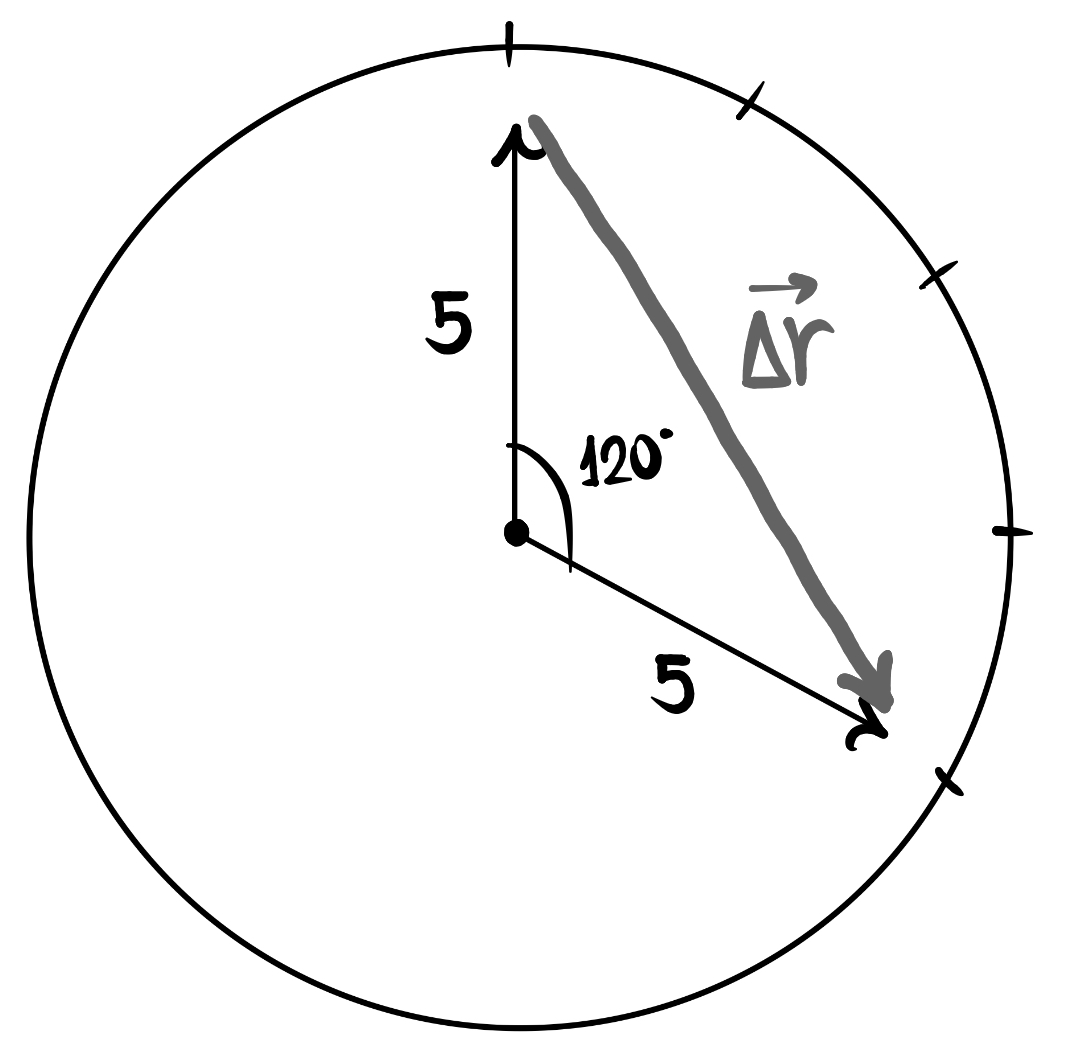
\includegraphics[width=0.3\linewidth]{imagenscinematicavetorial/relogio.jpeg}
\captionof{figure}{}
\label{fig_cinvet_ponteirorelogio}
} 

O vetor deslocamento $\Delta \vec{r}$ vai da posição inicial da extremidade do ponteiro até a sua posição final, e está indicado na mesma imagem. O módulo de tal vetor pode ser computado usando diretamente a Lei dos Cossenos, ou então, por um outro caminho, que consiste em perceber que tal triângulo é isósceles. \\

Assim, sendo seus lados iguais, os ângulos base também o serão, e iguais a $30^\circ$ no caso, para totalizar $180^\circ$ com o ângulo já encontrado de $120^\circ$. Sendo o triângulo isósceles, sua altura será também bissetriz, dividindo o ângulo de $120^\circ$ em dois iguais, e será também mediana, dividindo o módulo do vetor deslocamento em duas partes iguais, como mostra a Figura \ref{fig_cinvet_ponteirorelogio02}.

{
\centering
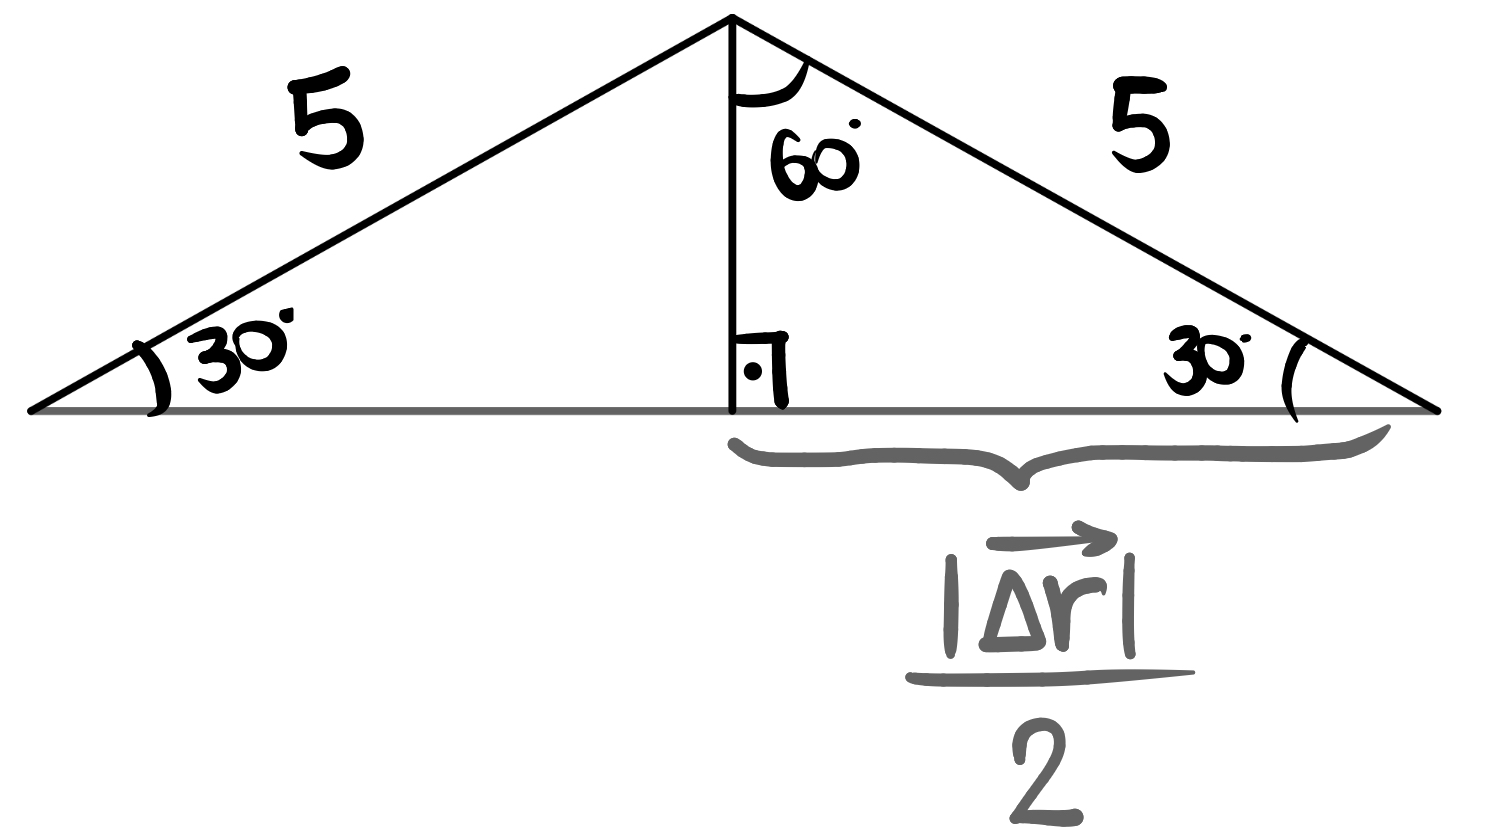
\includegraphics[width=0.3\linewidth]{imagenscinematicavetorial/ponteirorelogio02.jpeg}
\captionof{figure}{}
\label{fig_cinvet_ponteirorelogio02}
} 


Por meio de tal figura o cálculo se dá de forma imediata usando trigonometria básica:

$$ \sin 60^\circ = \dfrac{\sqrt3}{2}=\dfrac{\sfrac{|\Delta \vec{r}|}{2}}{5} \implies |\Delta \vec{r}| = 5\sqrt3 \text{ cm,}$$

\noindent de modo que a velocidade vetorial média é um vetor de módulo

$$ |\vec{v}_m| = \dfrac{|\Delta \vec{r}|}{\Delta t}= \dfrac{5 \sqrt 3 \text{ cm}}{20 \text{ min}} \implies \boxed{|\vec{v}_m| =\dfrac{\sqrt 3}{4} \text{ cm/min.}}$$
    
\end{exemplo}


\vspace{0.3cm}


\begin{exemplo}[Nível III (ITA 2009 - ADAPTADA)]\label{exemplo_cinematicavetorial_velocidadevetorialex03}

Na figura, um ciclista percorre o trecho $AB$ com velocidade escalar média de $22{,}5\ \text{km/h}$ e, em seguida, o trecho $BC$ de $3{,}00\ \text{km}$ de extensão.
No retorno, ao passar em $B$, verifica ser de $20{,}0\ \text{km/h}$ sua velocidade escalar média no percurso então percorrido, $ABCB$.
Finalmente, ele chega em $A$ perfazendo todo o percurso de ida e volta em $1{,}00\ \text{h}$, com velocidade escalar média de $24{,}0\ \text{km/h}$.
Encontre o módulo $v$ do vetor velocidade média referente ao percurso $ABCB$.

\vspace{0.8cm}

\begin{center}
\begin{tikzpicture}[scale=1.05, line cap=round, line join=round]
  % Points
  \coordinate (A) at (0,0);
  \coordinate (B) at (6,0);
  \coordinate (C) at (9,2.2);

  % Path AB (horizontal)
  \draw[thick] (A) -- (B);

  % Path BC (inclined)
  \draw[thick] (B) -- (C);

 

  % Labels
  \node[below] at (A) {$A$};
  \node[below] at (B) {$B$};
  \node[above right] at (C) {$C$};

  % Length label for BC
  \node[rotate=33.5, above] at ($(B)!0.55!(C)$) {$3{,}00\ \text{km}$};
\end{tikzpicture}
\end{center}




\resolucao

Seja $x$ o comprimento do segmento $\overline{AB}$. Como queremos o vetor velocidade média no trecho $ABCB$, vemos que o deslocamento total será o vetor $\overrightarrow{AB},$ uma vez que o ciclista sai de $A$ e termina em $B$. O módulo de tal vetor, sendo $x,$ faz com que o módulo da velocidade vetorial média em todo o trecho seja
$$ |\vec{v}_m| = \dfrac{|\Delta \vec{r}|}{\Delta t},$$

\noindent em que $\Delta t$ é o tempo de movimento do trecho ABCB.\\

Avaliemos a velocidade média no trecho total ABCBA, de 1 hora de duração. Como o enunciado nos diz que a velocidade escalar média em tal trecho é de $24$ km/h, teremos:

$$ v_m = 24 = \dfrac{d}{t} = \dfrac{x+3+3+x}{1} \implies x = 9 \text{ km.}$$

Avaliando o trecho $ABCB,$ sendo de $20,0$ km/h sua velocidade escalar média em tal trecho, temos que sua duração foi de

$$\Delta t = \dfrac{d}{v} = \dfrac{(9+3+3) \text{ km}}{20 \text{ km/h}}= \dfrac{3}{4} \text{ h.}$$

Logo, a velocidade vetorial média no trecho ABCB tem módulo dado por

  $$ |\vec{v}_m| = \dfrac{|\Delta \vec{r}|}{\Delta t} = \dfrac{x}{\Delta t}=\dfrac{9 \text{ km}}{\sfrac{3}{4} \text{ h} } = \boxed{12 \text{ km/h.}}$$
    
\end{exemplo}


\vspace{0.3cm}










\section{Aceleração Vetorial}






\begin{secnivel}[Aceleração Vetorial Média]{I}{Aceleração Vetorial Média}
  
  \eqLdois{def}{cinvet_eq_aceleracaovetorialmedia}{\vec{a}_m  := \dfrac{\Delta \vec{v}}{\Delta t}}

\end{secnivel}




\secgfe{De onde vem}

Essa definição é apenas uma continuação do conceito de aceleração escalar média, em que agora estendemos esse conceito para absorver o caráter vetorial da velocidade.

Assim, tendo definido a velocidade vetorial, fica natural definir a aceleração vetorial média como sendo a variação de tal grandeza no tempo, ou seja:

$$ \vec{a}_m = \dfrac{\Delta \vec{v}}{\Delta t} = \dfrac{\vec{v}-\vec{v_0}}{t-t_0},$$

\noindent em que $\vec{v}$ é a velocidade do objeto no instante $t,$ e $\vec{v}_0$ é a velocidade do objeto no instante $t_0.$

Como já investimos muito tempo em discutir qual é o sentido em se definir a aceleração média como o fizemos -- na parte sobre Cinemática Escalar -- parece razoável ser mais sucinto nesse momento. A lógica agora é realmente apenas ampliar tal conceito para incorporar o caráter vetorial da velocidade.


\secgfe{Onde é usada}

Tal como comentamos acerca de Equação \eqref{cinvet_eq_velocidadevetorialmedia}, algo semelhante se aplica à Equação \eqref{cinvet_eq_aceleracaovetorialmedia}: ela é, de forma direta, bem pouco usada. Será raro o leitor se deparar com algum contexto físico, problema ou exercício em que ele precise usar diretamente tal equação.

Ela, contudo, é usada como passo intermediário para construir outras equações que usaremos mais, como, por exemplo, a da aceleração centrípeta. Sendo assim, a importância da Equação \eqref{cinvet_eq_aceleracaovetorialmedia} se dará mais pelo que decorrerá dela do que do uso direto em si.


\secgfe{Erros comuns}

Os erros mais comuns aqui costumam ser de geometria ou trigonometria. Como a equação em questão é vetorial, o cálculo de $\Delta \vec{v}$ envolve a subtração de dois vetores -- a velocidade final e inicial. Logo, a geometria de tal cálculo irá depender da direção desses vetores, e o seu cálculo poderá envolver alguns teoremas da geometria plana como o Teorema de Pitágoras, a Lei dos Senos e Cossenos, ou noções básicas de trigonometria como aplicação de seno, cosseno e tangente em triângulos retângulos.

O leitor que não estiver muito afiado nesses conceitos possivelmente encontrará dificuldades em fazer cálculos envolvendo a Equação \eqref{cinvet_eq_aceleracaovetorialmedia}



\secgfe{Observações}

Como pontuamos, o que estamos fazendo aqui é apenas uma extensão do conceito escalar de aceleração. Assim, é interessante notar que essa nova definição de aceleração média incorpora, como casos particulares, o que já conhecíamos como aceleração. 

Note, por exemplo, o movimento da Figura \ref{fig_cinvet_aceleracaovetorialecasoparticular1}, que mostra um MU em linha reta. Como sabemos, em tal movimento a aceleração é nula, o que de fato ocorre caso façamos o cálculo por meio da Equação \eqref{cinvet_eq_aceleracaovetorialmedia}, como é mostrado no lado direito da figura. Ali, tomamos o instante final $t=2$s e sua velocidade ali, cujo módulo é $|\vec{v}_f|=2$ m/s, apontando para a direita. Já a velocidade inicial $\vec{v}_0$ é aquela em $t=0$s, cujo módulo é $|\vec{v}_0|=2$ m/s e também aponta para direita. 

Assim, fazendo a variação $\Delta \vec{v} = \vec{v_f}-\vec{v}_0,$ chegamos, naturalmente, em um vetor nulo, de modo que a aceleração vetorial média será $\sfrac{\Delta \vec{v}}{\Delta t}= \vec 0,$ como esperado\footnote{Usamos aqui o zero como vetor para manter a coerência: do lado esquerdo da equação temos um vetor, calculado por $\sfrac{\Delta \vec{v}}{\Delta t}$, de modo que o lado direito também deve ser o vetor. O vetor $\vec 0$ é o vetor nulo: seu módulo é zero, de modo que sua direção e sentido são irrelevantes haja vista que ele não aponta para lugar algum.}. Caso o leitor avalie em quaisquer outros intervalos de tempo chegará sempre no mesmo resultado, e a conclusão -- que já sabíamos, mas sem usar o caráter vetorial até então -- é de que a aceleração é nula ao longo do Movimento Uniforme.

\vspace{0.3cm}

{
\centering
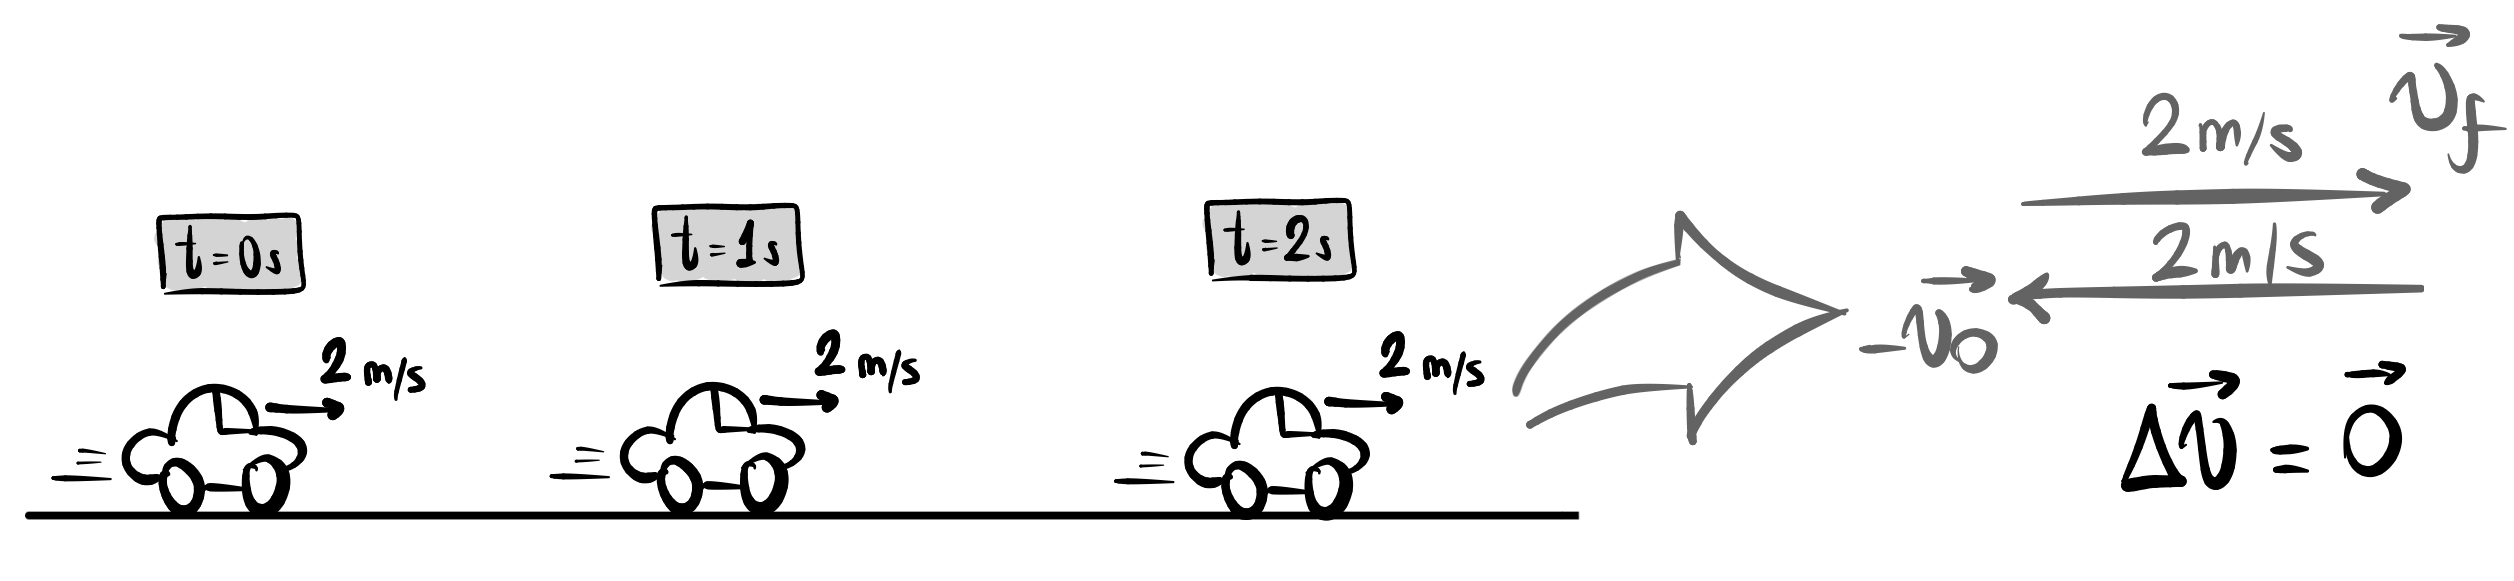
\includegraphics[width=0.85\linewidth]{imagenscinematicavetorial/aceleracaovetorialecasoparticular1.jpeg}
\captionof{figure}{O conceito de aceleração vetorial média aplicada ao Movimento Uniforme em linha reta.}
\label{fig_cinvet_aceleracaovetorialecasoparticular1}
} 

\vspace{0.3cm}

Um outro caso particular pode ser observado na Figura \ref{fig_cinvet_aceleracaovetorialecasoparticular2}, que mostra um Movimento Uniformemente Variado em linha reta. Novamente, tomamos o instante final $t=2$s e sua velocidade ali, cujo módulo é $|\vec{v}_f|=1$ m/s, apontando para a direita. Já a velocidade inicial $\vec{v}_0$ é aquela em $t=0$s, cujo módulo é $|\vec{v}_0|=7$ m/s e também aponta para direita. 

\vspace{0.3cm}

{
\centering
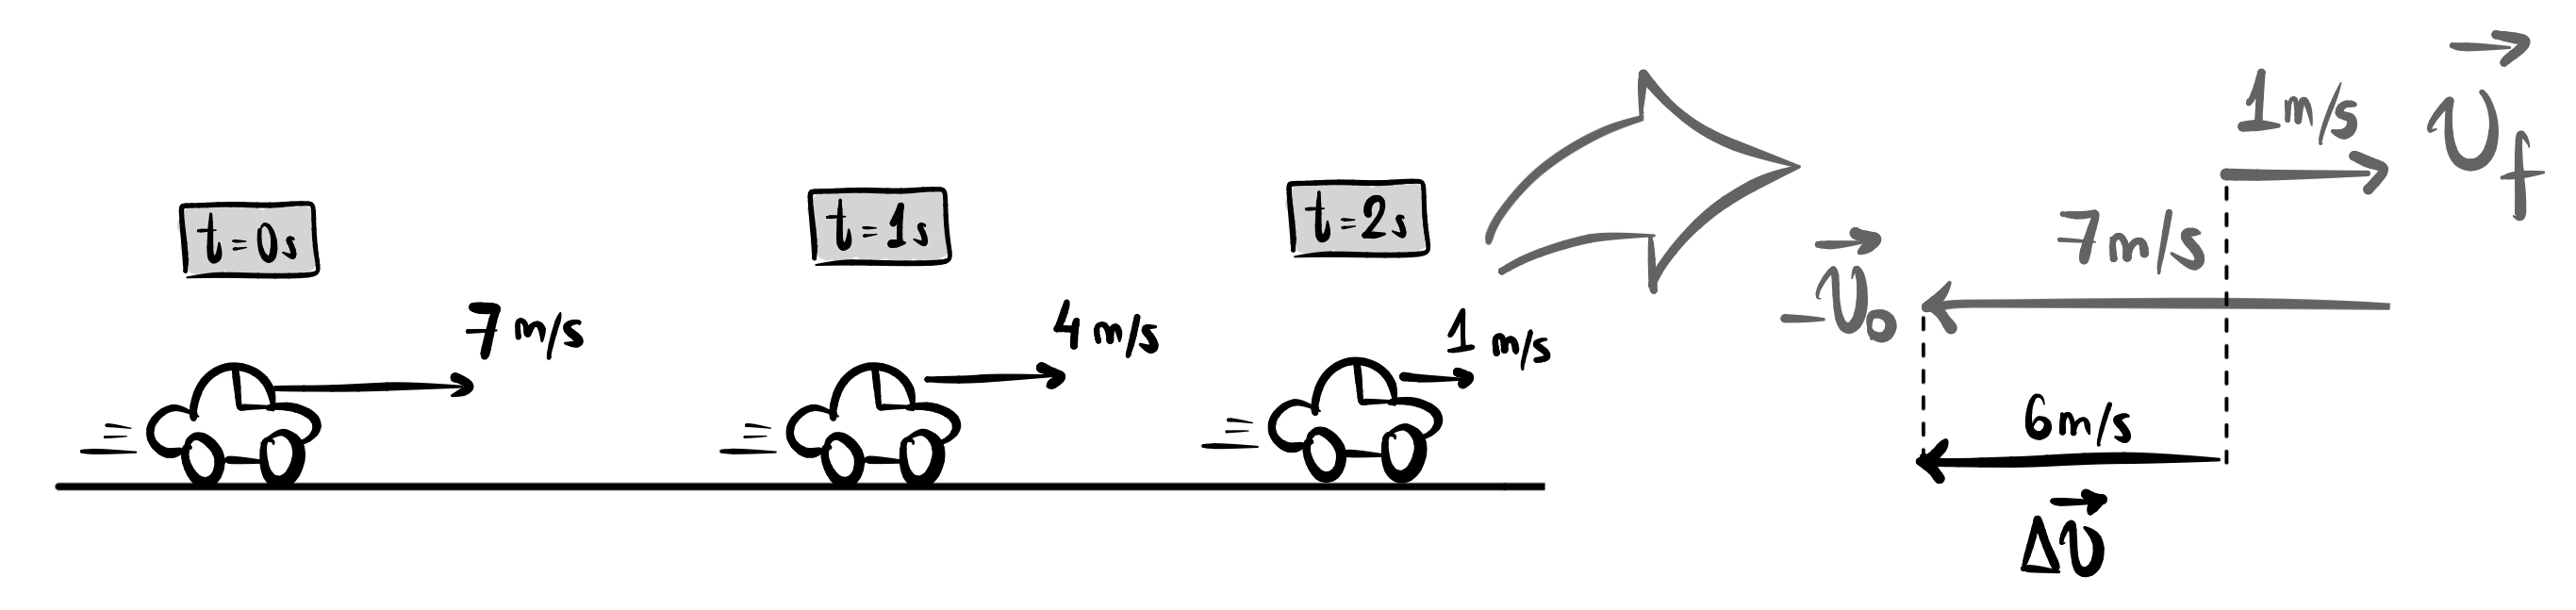
\includegraphics[width=0.8\linewidth]{imagenscinematicavetorial/aceleracaovetorialecasoparticular2.jpeg}
\captionof{figure}{O conceito de aceleração vetorial média aplicada ao Movimento Uniformemente Variado em linha reta.}
\label{fig_cinvet_aceleracaovetorialecasoparticular2}
} 

\vspace{0.3cm}

O lado direito da imagem mostra o esboço do cálculo da variação $\Delta \vec{v} = \vec{v_f}-\vec{v}_0,$ que resulta em um vetor de tamanho $6$, isto é, $|\Delta \vec{v}|=6$ m/s, porém apontando para a esquerda. Assim, a aceleração vetorial média nos dois segundos de movimento tem módulo igual a

$$ |\vec{a}_m| = \dfrac{|\Delta \vec{v}|}{\Delta t} = \dfrac{6 \text{ m/s}}{2 \text{ s}} \implies \boxed{ |\vec{a}_m|=3 \text{ m/s$^2$},}$$

\noindent apontando para a esquerda -- que é o sentido do vetor $\Delta \vec{v}$ --, de modo que o movimento é retardado. Calculando a aceleração entre quaisquer dois instantes de tempo -- e usando a definição escalar de aceleração -- o leitor será levado ao mesmo resultado.

Com isso, fica claro que nossa nova definição de aceleração média incorpora todo o conceito de aceleração que já conhecíamos, e, na verdade, estende-o para um campo de aplicação ainda maior, uma vez que, com o caráter vetorial embutido na definição, poderemos tratar de movimentos bidimensionais, o que antes não era possível.

\vspace{0.3cm}
%Exemplo resolvido

\begin{exemplo}[Nível I]\label{exemplo_cinematicavetorial_aceleracaovetorialexemplo01}

Considere a situação ilustrada na Figura \ref{fig_cinvet_aceleracaovetorialmediaex01}. Calcule, entre os instantes $t=0$s e $t=2$s, a aceleração escalar média do corpo e a sua aceleração vetorial média.

{
\centering
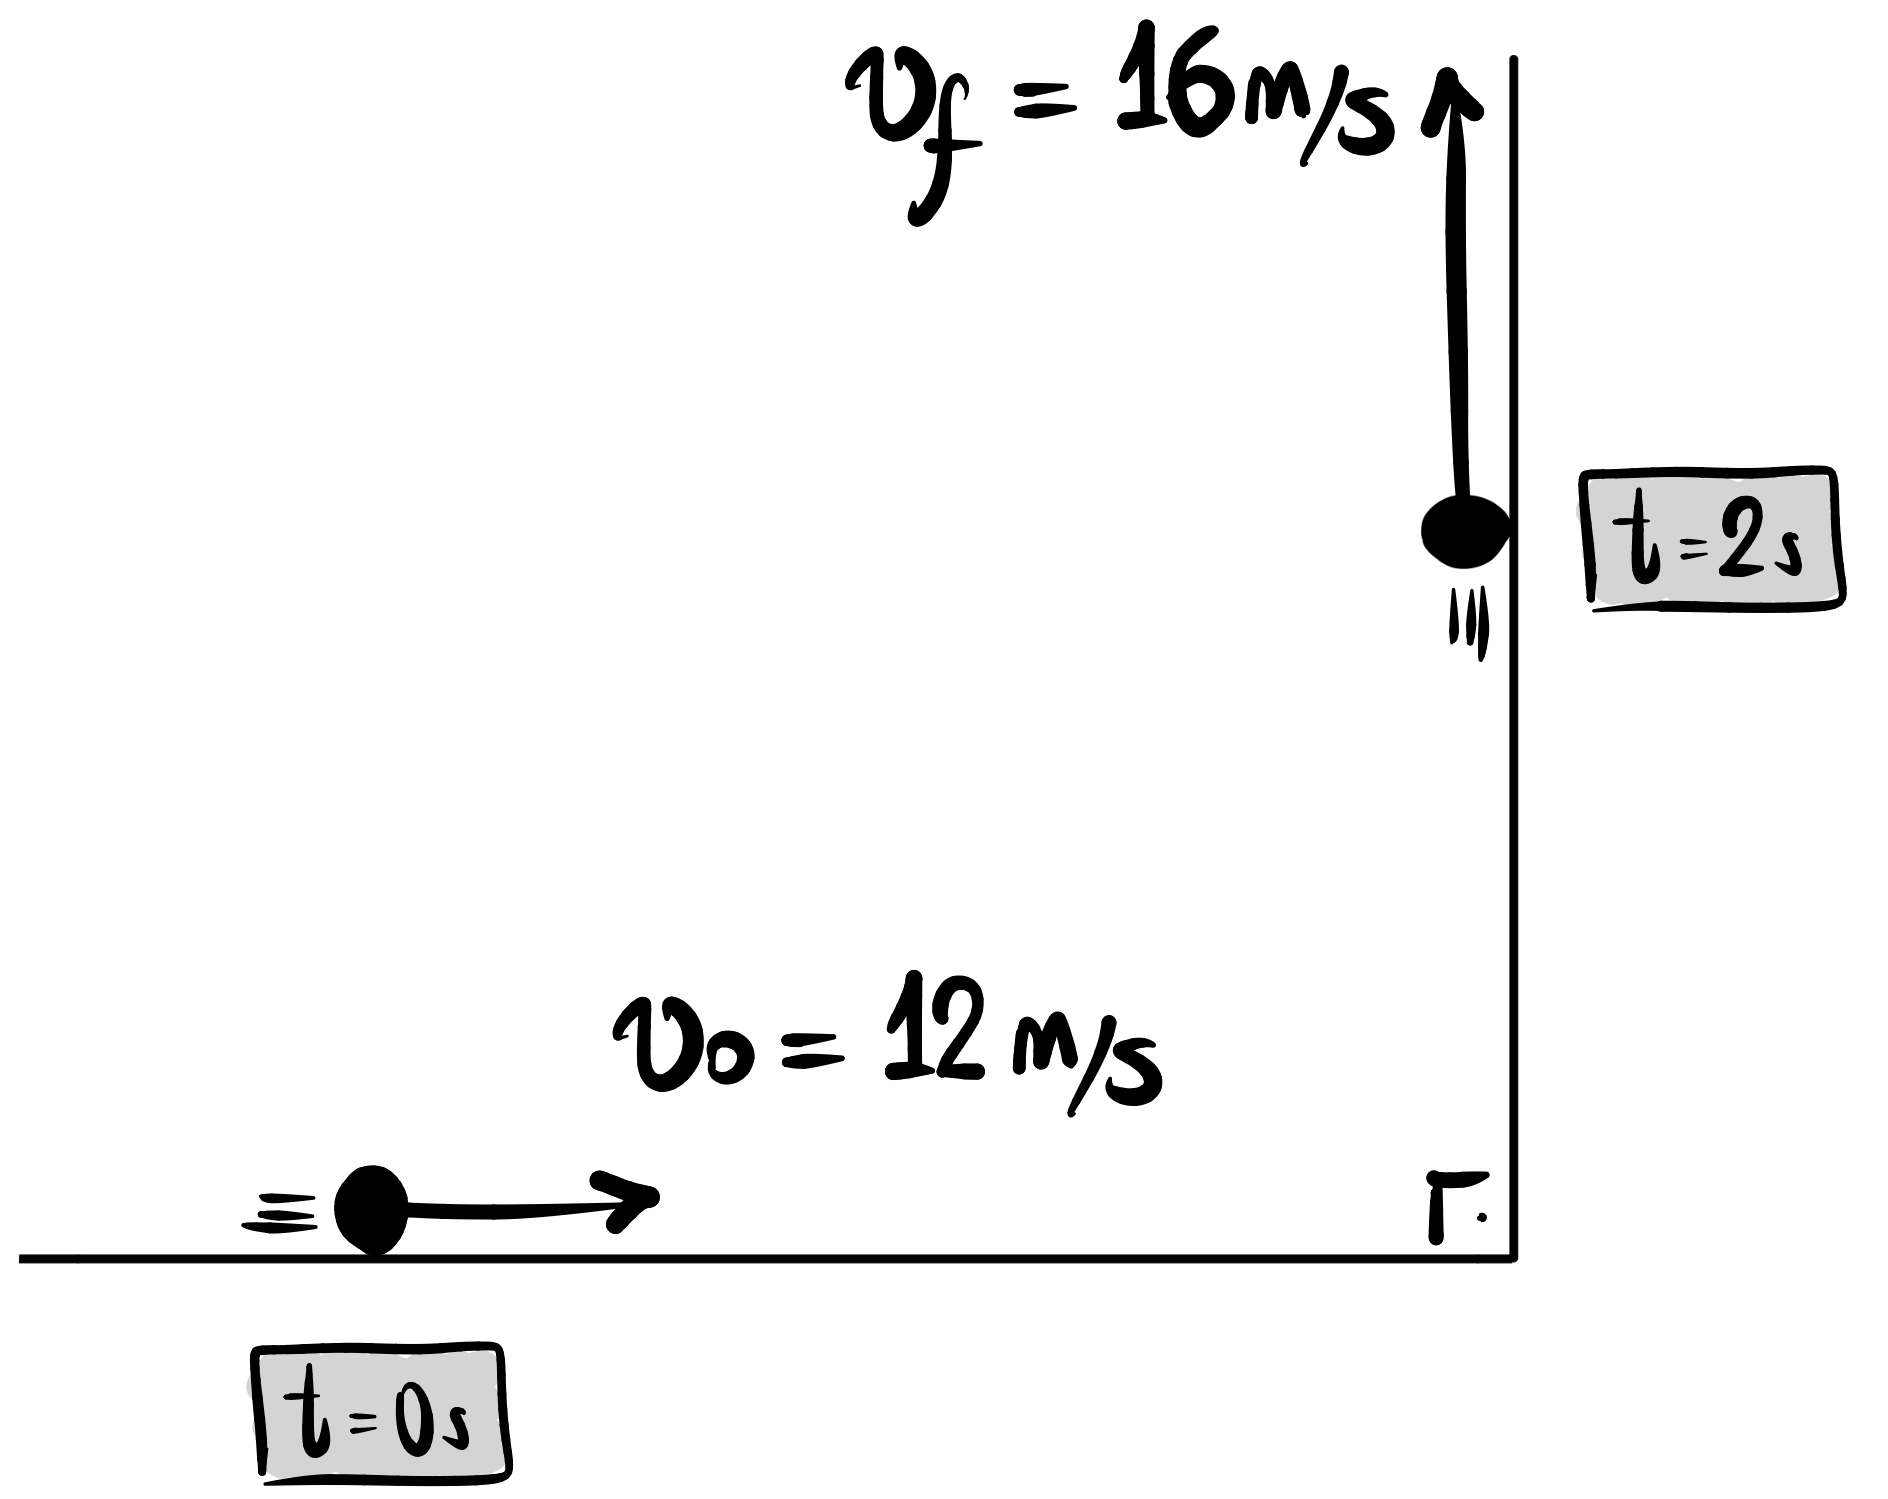
\includegraphics[width=0.35\linewidth]{imagenscinematicavetorial/aceleracaovetorialmediaex01.jpeg}
\captionof{figure}{}
\label{fig_cinvet_aceleracaovetorialmediaex01}
} 

\resolucao


Este é UM ótimo exemplo para percebermos a diferença entre a aceleração vetorial e a aceleração escalar. Faremos aqui, portanto, uma extensa digressão a fim de tornar clara essa diferença e suas nuances. Vamos por partes:

\begin{enumerate}
    \item [(a)] Aceleração Escalar Média

    Essa grandeza mede apenas o quanto varia o valor, isto é, o módulo, da velocidade. Sendo assim, seu cálculo é imediato:

    $$ a_m=\dfrac{\Delta v}{\Delta t}=\dfrac{16-12}{2-0} \implies \boxed{a_m=2 \text{ m/s$^2$.}}$$


     \item [(b)] Aceleração Vetorial Média

     Agora o que importa não são apenas os valores, isto é, os módulos das velocidades, mas também sua direção e sentido, já que elas influenciarão na geometria do problema. Observe a Figura \ref{fig_cinvet_aceleracaovetorialmediaex012}, que esboça o cálculo de $\Delta \vec{v}=\vec{v}_f-\vec{v}_0.$

{
\centering
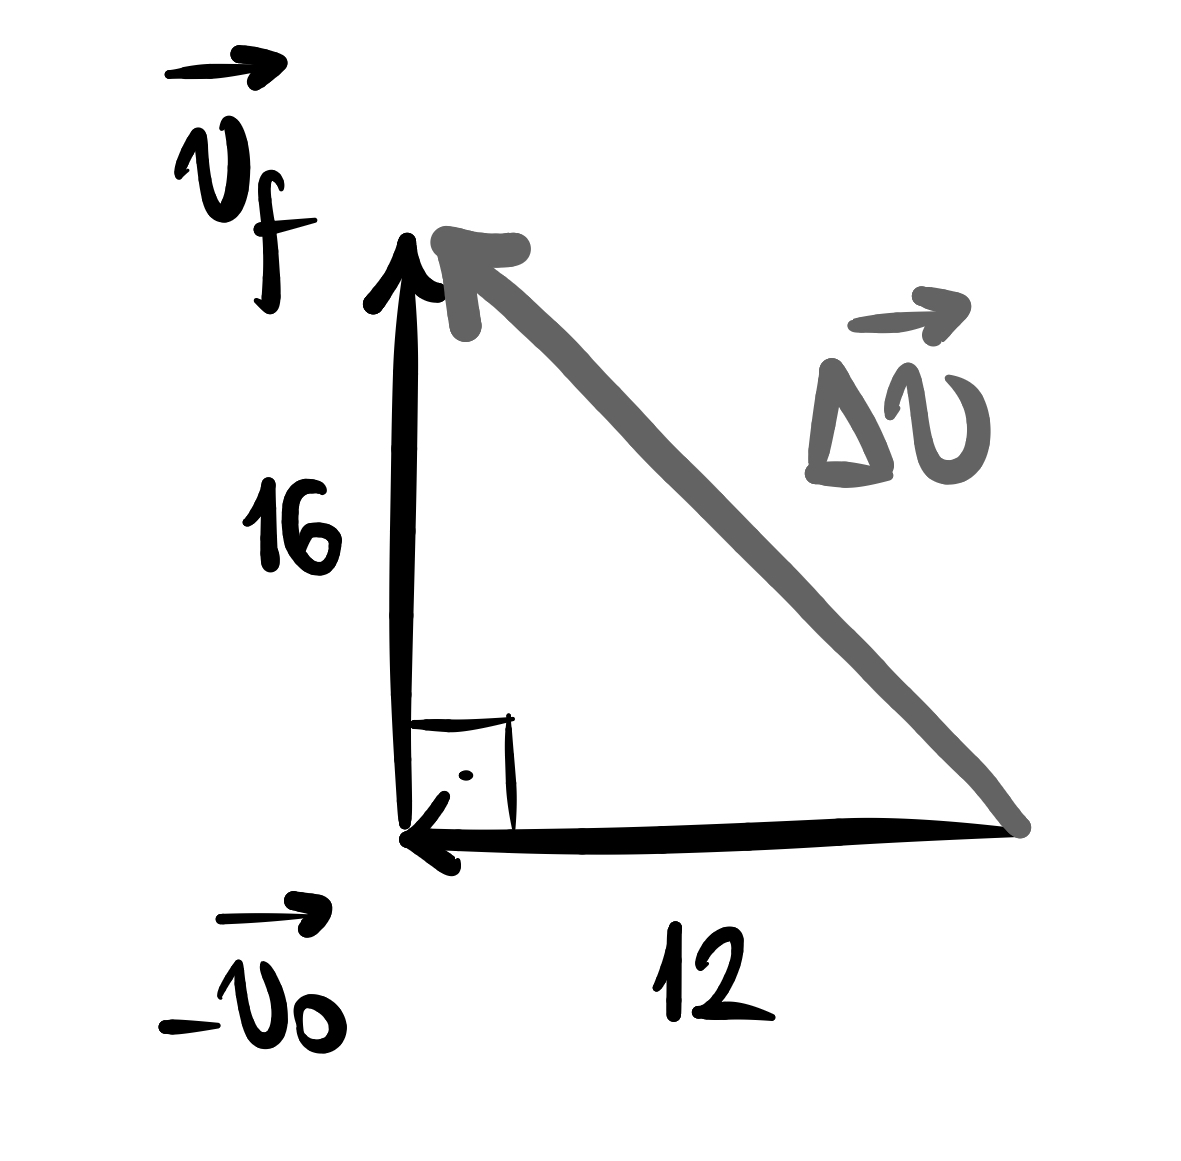
\includegraphics[width=0.25\linewidth]{imagenscinematicavetorial/aceleracaovetorialmediaex012.jpeg}
\captionof{figure}{}
\label{fig_cinvet_aceleracaovetorialmediaex012}
} 

A partir de tal figura é imediato calcular o módulo da variação da velocidade, que é obtido pelo Teorema de Pitágoras:

$$ |\Delta \vec{v}|^2 = 12^2+16^2 \implies |\Delta \vec{v}| = 20 \text{ m/s},$$

\noindent de modo que o módulo da aceleração vetorial média é

$$ |\vec{a}_m| = \dfrac{|\Delta \vec{v}|}{\Delta t} = \dfrac{20 \text{ m/s}}{2 \text{ s}} \implies \boxed{|\vec{a}_m|=10 \text{ m/s$^2$}.}$$

     
\end{enumerate}

Pois bem...as respostas não coincidiram. Em um primeiro momento isso pode parecer estranho, mas, na verdade era algo a se esperar. Cabe destacarmos algumas observações importantes sobre este fato:


\begin{enumerate}
    \item [(i)] Coincidência entre os cálculos escalar e vetorial.

    Os valores da aceleração escalar e do módulo da aceleração vetorial só vão coincidir em movimentos unidimensionais, como já exposto. Na seção sobre \textbf{observações} a respeito da Equação \eqref{cinvet_eq_velocidadevetorialmedia} deixamos isso claro com os exemplos do MU e do MUV em linha reta. 
    
    A questão, no contexto deste exemplo, é que o movimento muda de direção -- e a aceleração escalar não consegue capturar essa informação. Observe que, do ponto de vista da aceleração escalar, as velocidades da Figura \ref{fig_cinvet_axeaxyaceleracaovetorial1} são iguais -- duas velocidades cujo valor é de $10$ m/s. 

{
\centering
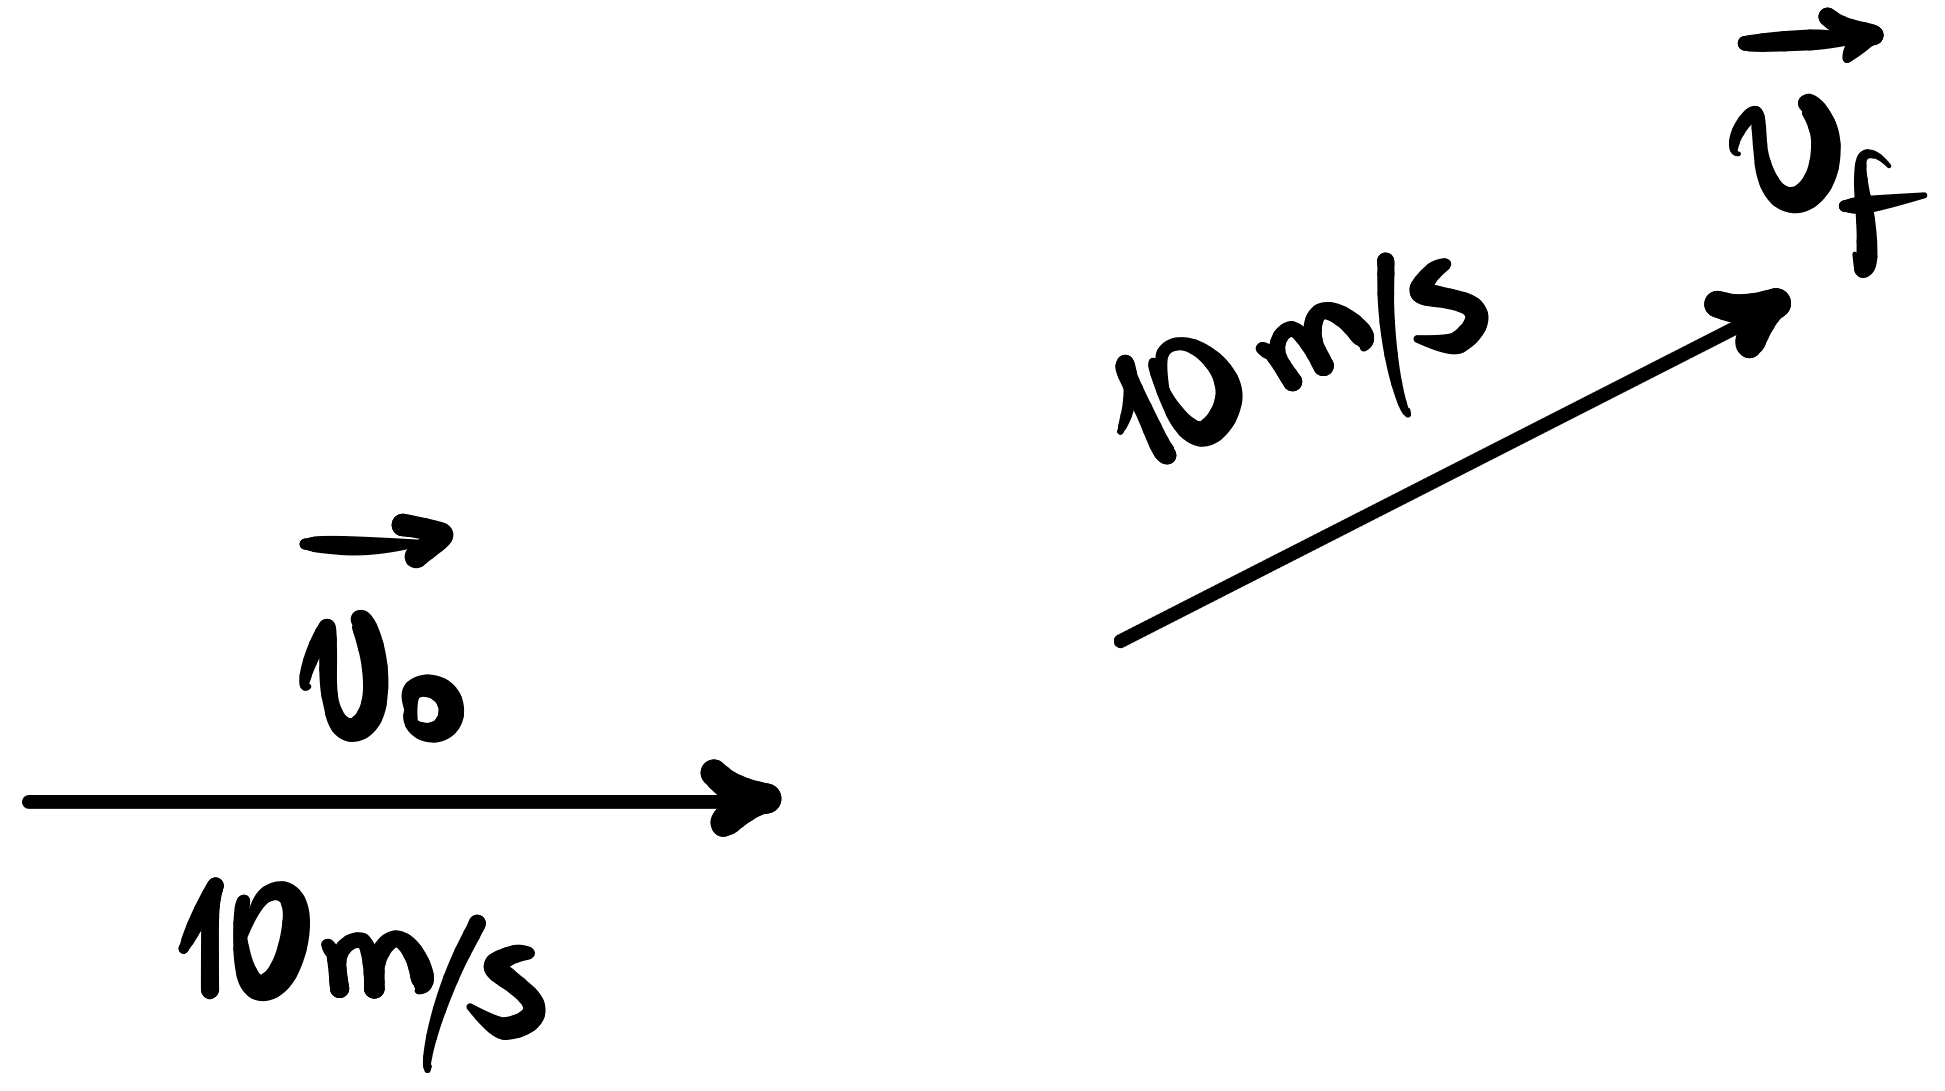
\includegraphics[width=0.30\linewidth]{imagenscinematicavetorial/axeaxyaceleracaovetorial1.jpeg}
\captionof{figure}{}
\label{fig_cinvet_axeaxyaceleracaovetorial1}
} 
    
    
    \item [(ii)] Caráter vetorial da velocidade.

    O fato de termos obtido valores distintos para as acelerações neste exemplo é por que, enquanto a aceleração escalar só percebe a variação do valor da velocidade, que foi de $16-12=4$ m/s, a aceleração vetorial captura também a variação vetorial da velocidade, isto é, a variação da sua direção. Voltemos, por exemplo, ao caso da Figura \ref{fig_cinvet_axeaxyaceleracaovetorial1}. Digamos que a velocidade $\vec{v}_f$ faça um ângulo $\theta$ com a horizontal -- direção da velocidade $\vec{v}_0$ -- tal que  $\sin \theta = 0.6 \quad \text{ e } \quad \cos \theta = 0.8.$ 
    
    Neste caso, obtemos, por trigonometria básica, que

    $$ \sin \theta = \dfrac{v_y}{10}=0.6 \implies \boxed{v_y= 6 \text{ m/s}} \quad \text{ e } \quad \cos \theta = \dfrac{v_x}{10}=0.8 \implies \boxed{v_x= 8 \text{ m/s},}$$
    
\noindent como mostra a Figura \ref{fig_cinvet_axeaxyaceleracaovetorial2}.

{
\centering
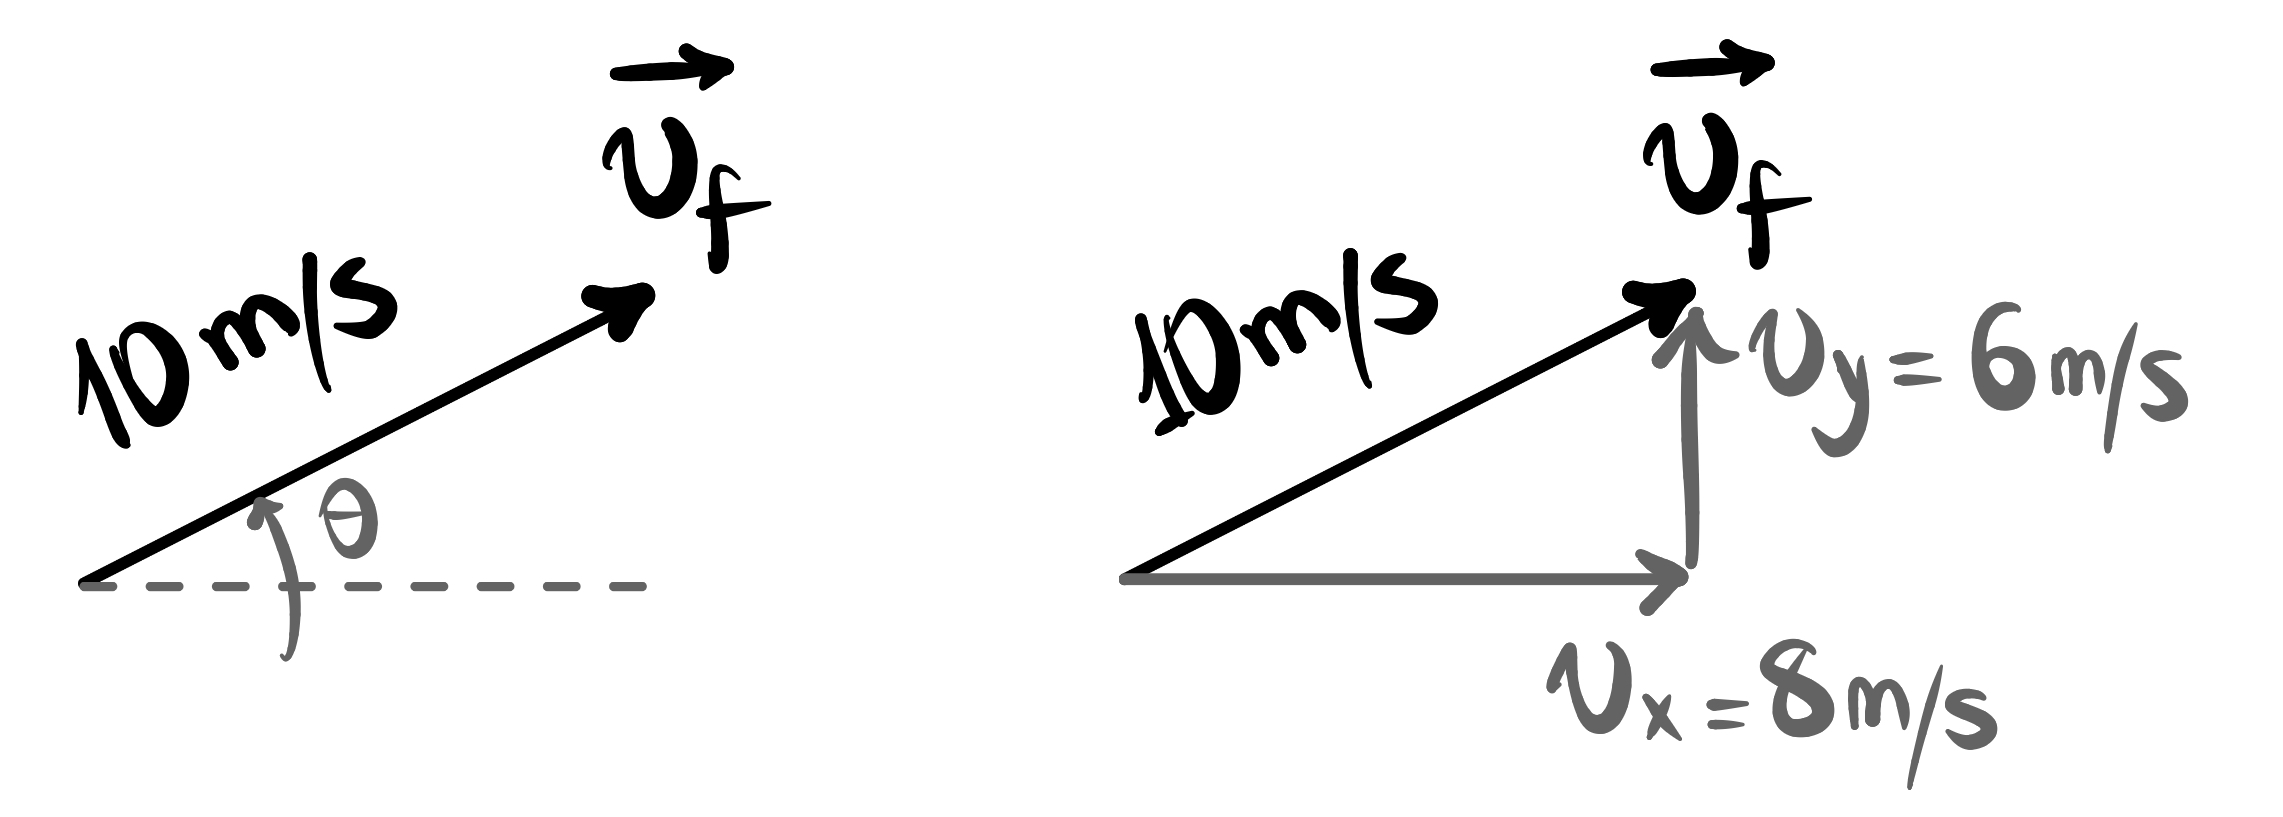
\includegraphics[width=0.50\linewidth]{imagenscinematicavetorial/axeaxyaceleracaovetorial2.jpeg}
\captionof{figure}{}
\label{fig_cinvet_axeaxyaceleracaovetorial2}
} 

Assim, a velocidade $\vec{v}_f$ pode ser interpretada como composta por uma velocidade horizontal $\vec{v}_x$ cujo módulo é de $8$ m/s, e uma velocidade vertical $\vec{v}_y$ cujo módulo é de $6$ m/s. Neste caso, comparar as velocidades $\vec{v}_0$ e $\vec{v}_f$ da Figura \ref{fig_cinvet_axeaxyaceleracaovetorial1} deixa evidente como elas são diferentes, como destaca a Figura \ref{fig_cinvet_axeaxyaceleracaovetorial3}.



{
\centering
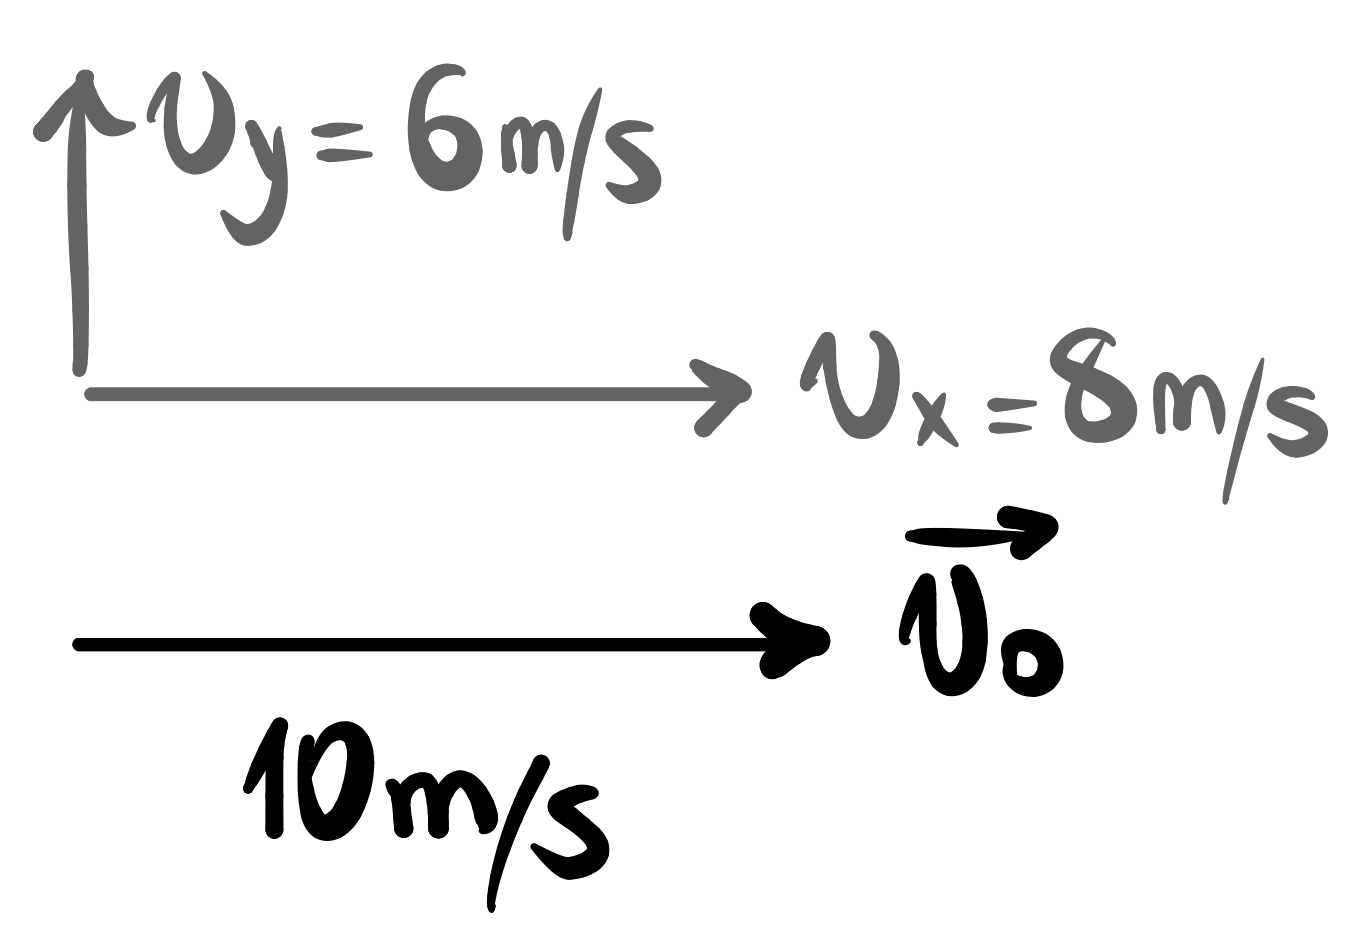
\includegraphics[width=0.30\linewidth]{imagenscinematicavetorial/axeaxyaceleracaovetorial3.jpeg}
\captionof{figure}{}
\label{fig_cinvet_axeaxyaceleracaovetorial3}
} 

Para alterar a velocidade do seu estado inicial $\vec{v_0}$ e fazer com que se chegue no estado final $\vec{v}_f$ \textbf{é preciso alterar seu valor em duas dimensões}: diminuir em $2$ m/s a componente horizontal e aumentar em $6$ m/s a componente vertical. 

E é por isso que a aceleração escalar fornece um resultado diferente: ela ignora o caráter bidimensional do movimento por olhar apenas para o valor absoluto da velocidade, e não para o que acontece com a velocidade enquanto ente geométrico.

    \item [(iii)] Análise por componentes.

Uma perspectiva final que vale pontuar é que a aceleração vetorial pode ser interpretada, no contexto deste problema, como uma espécie de aceleração escalar composta em duas dimensões. 

Voltando ao problema do exemplo e avaliando o movimento separadamente nas suas componentes horizontal e vertical, como fizemos no final do tópico acima, podemos entender que, para sair do estado inicial e chegar no estado final, é preciso desacelerar completamente na horizontal, indo de $v_{0}=12$ m/s até $0$ m/s, o que exigiria uma variação de velocidade horizontal de

$$ \Delta v_x  =0-12 = -12\text{ m/s},$$

\noindent o que significa, no intervalo de tempo de $2$s, haver uma aceleração horizontal $a_x$ que retarda a partícula dada por

$$a_x=\dfrac{\Delta v_x}{\Delta t} = \dfrac{-12 \text{ m/s}}{2\text{ s}} = -6 \text{ m/s$^2$},$$

\noindent em que o sinal negativo só indica que aceleração possui sentido contrário ao da velocidade inicial, ou seja, o movimento de fato é retardado.

{
\centering
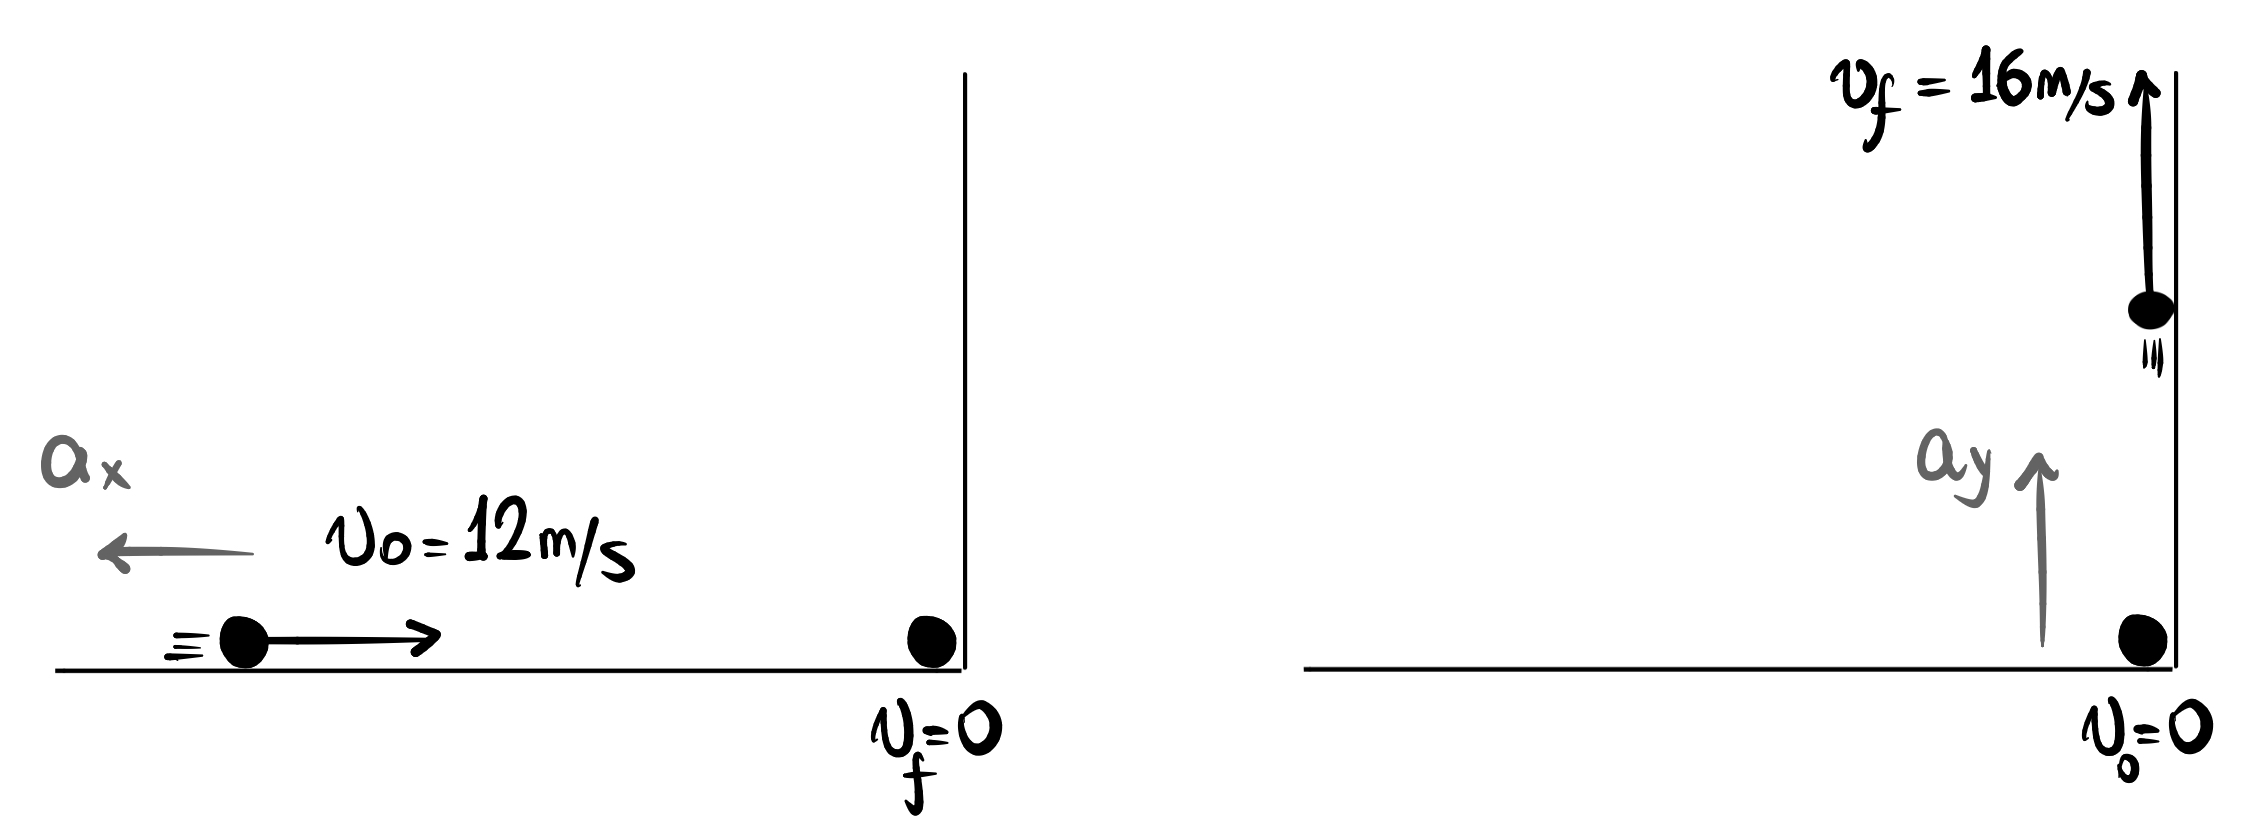
\includegraphics[width=0.80\linewidth]{imagenscinematicavetorial/axeaxyaceleracaovetorial4.jpeg}
\captionof{figure}{}
\label{fig_cinvet_axeaxyaceleracaovetorial4}
} 


Após ter desacelerado totalmente na horizontal, é preciso agora que a nossa partícula, saindo do repouso, adquira uma velocidade de $16$ m/s na direção vertical, a fim de alcançar o estado final de movimento do contexto. Assim, haverá uma variação de velocidade vertical dada por

$$\Delta v_y  = 16-0 = 16\text{ m/s}, $$

\noindent o que significa, no intervalo de tempo de $2$s, haver uma aceleração vertical $a_y$ que acelere a partícula dada por

$$a_y=\dfrac{\Delta v_y}{\Delta t} = \dfrac{16 \text{ m/s}}{2\text{ s}} = 8 \text{ m/s$^2$}.$$

Tal situação aparece ilustrada na Figura \ref{fig_cinvet_axeaxyaceleracaovetorial4}, em que imaginamos o movimento completo como sendo uma desaceleração horizontal $a_x$ que leva a partícula até o repouso logo antes de encostar na parede e, na sequência, uma aceleração vertical $a_y$ que tira a partícula do repouso e a leva à velocidade vertical de $16$ m/s. 

Quebramos o movimento nesses dois estágios para fins didáticos, mas as duas coisas acontecem ao mesmo tempo -- enquanto a partícula desacelera na horizontal ela acelera na vertical -- de modo que o tempo no qual as ``duas acelerações'' atuam é o mesmo, o tempo total de $2$ segundos do movimento completo.


{
\centering
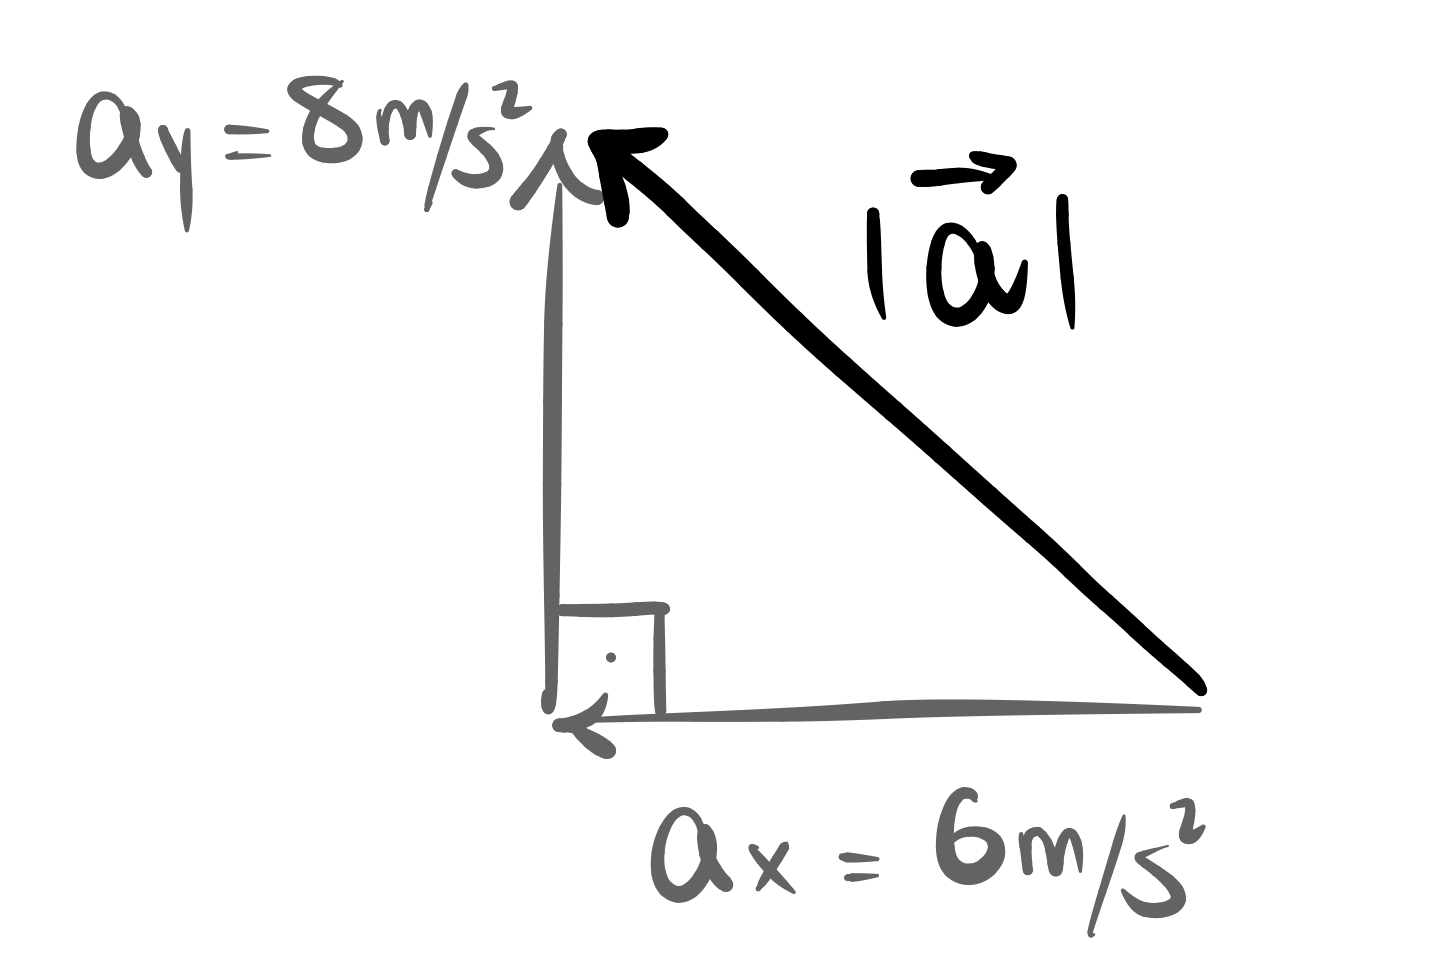
\includegraphics[width=0.30\linewidth]{imagenscinematicavetorial/fig_cinvet_axeaxyaceleracaovetorial5.jpeg}
\captionof{figure}{}
\label{fig_cinvet_axeaxyaceleracaovetorial5}
} 

Sendo assim, encontraríamos que a aceleração total do objeto seria o efeito resultante das acelerações $a_x$ e $a_y$, dado, pelo Teorema de Pitágoras no triângulo da Figura \ref{fig_cinvet_axeaxyaceleracaovetorial5}:

$$ |\vec{a}_m|^2 = a_x^2+a_y^2 = 6^2+8^2 \implies \boxed{|\vec{a}_m|=10 \text{ m/s$^2$}.}$$

Note que este foi o mesmo resultado obtido no cálculo do item $(b)$ do exemplo, porém agora usando, em cada dimensão, o conceito de aceleração escalar. Convida-se, neste momento, o leitor a comparar a Figura \ref{fig_cinvet_aceleracaovetorialmediaex012} com a figura acima, de modo a concluir que, em certa medida, a aceleração vetorial é uma superposição -- em duas dimensões -- do conceito de aceleração escalar, o qual só se aplicava para uma dimensão.
    
\end{enumerate}

    
\end{exemplo}


\vspace{0.3cm}


\begin{exemplo}[Nível II]\label{exemplo_cinvet_acelvetorialnivel2}

Considere um objeto que se move com uma velocidade de valor constante e igual a $10$m/s ao longo de uma trajetória circular. Se o objeto leva $12$ segundos para completar uma volta, calcule o módulo da sua aceleração vetorial média entre 

\begin{enumerate}
    \item [(a)] $t_1=3$s e $t_2=15$s.
    \item [(b)] $t_1=3$s e $t_2=9$s.
    \item [(c)] $t_1=3$s e $t_2=6$s.
    \item [(d)] $t_1=3$s e $t_2=5$s.
\end{enumerate}


\resolucao


Vale destacar que, como o objeto possui velocidade de módulo constante, a aceleração escalar seria zero qualquer que fosse o intervalo de tempo considerado. Assim, o que computarmos aqui como módulo da aceleração vetorial será relativo à aceleração responsável por variar a direção do vetor velocidade, e não o seu módulo, uma vez que este é constante em todo o movimento.

Vamos avaliar cada item separadamente:

\begin{enumerate}
    \item [(a)]  Perceba que os valores específicos dos instantes de tempo são pouco relevantes, o que importa é o intervalo de tempo. Para o primeiro caso, por exemplo, temos $\Delta t = t_2-t_1=15-3=12$s, ou seja, a partícula terá completado uma volta completa.

    Logo, as posições inicial e final sendo as mesmas, os vetores velocidade inicial também o serão, de modo que a sua variação será nula, e, sendo $|\Delta \vec{v}|=0,$ a aceleração vetorial média será nula neste intervalo de tempo.

    \item [(b)] Neste caso o intervalo de tempo é $\Delta t = t_2-t_1=9-3=6$s, de modo que a partícula terá completado meia volta, situação ilustrada na Figura \ref{fig_cinvet_aceleracaovetorialmediaexemplo0101}. 
    
    
    
    {
\centering
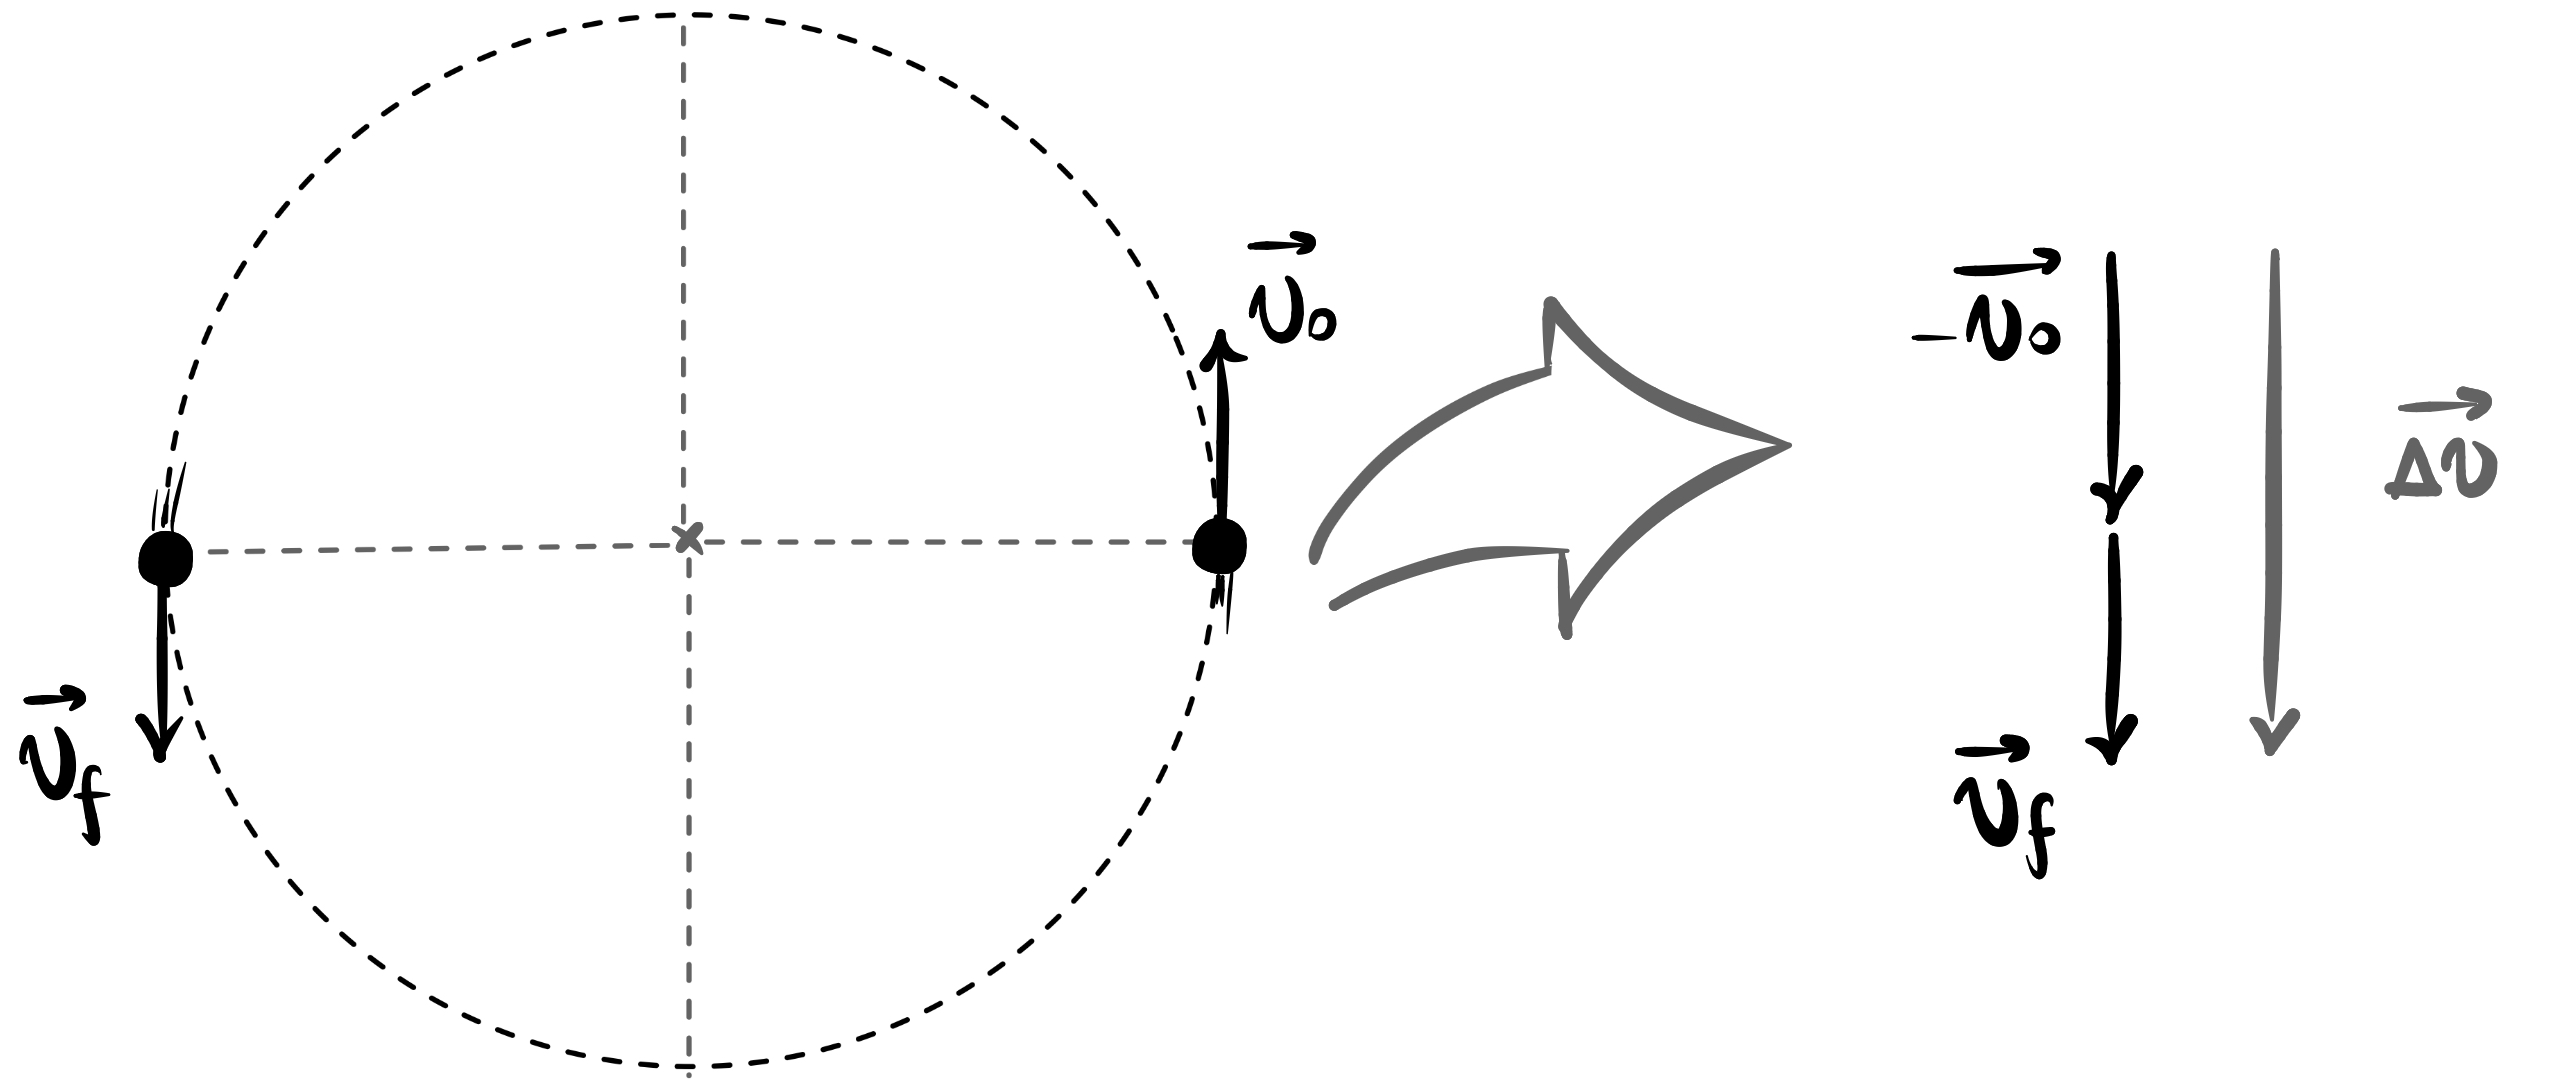
\includegraphics[width=0.6\linewidth]{imagenscinematicavetorial/fig_cinvet_aceleracaovetorialmediaexemplo0101.jpeg}
\captionof{figure}{}
\label{fig_cinvet_aceleracaovetorialmediaexemplo0101}
} 
    
    
    À direita na figura tem o esboço do cálculo de $\Delta \vec{v}=\vec{v}_f-\vec{v}_0,$ que, como se vê, terá módulo igual à soma dos módulos de $\vec{v}_0$ e $\vec{v}_f$, ou seja, $|\Delta \vec{v}|=10+10=20$m/s, de modo que a aceleração vetorial média é, neste intervalo, dada por

    $$ | \vec{a}_m|= \dfrac{|\Delta \vec{v}|}{\Delta t}= \dfrac{20 \text{ m/s}}{6\text{ s}} \implies \boxed{| \vec{a}_m|=\dfrac{10}{3}\text{ m/s$^2$}.}$$
     



   \item [(c)] Agora o intervalo de tempo é $\Delta t = t_2-t_1=6-3=3$s, de modo que a partícula terá completado um quarto de volta, situação ilustrada na Figura \ref{fig_cinvet_aceleracaovetorialmediaexemplo0102}.

{
\centering
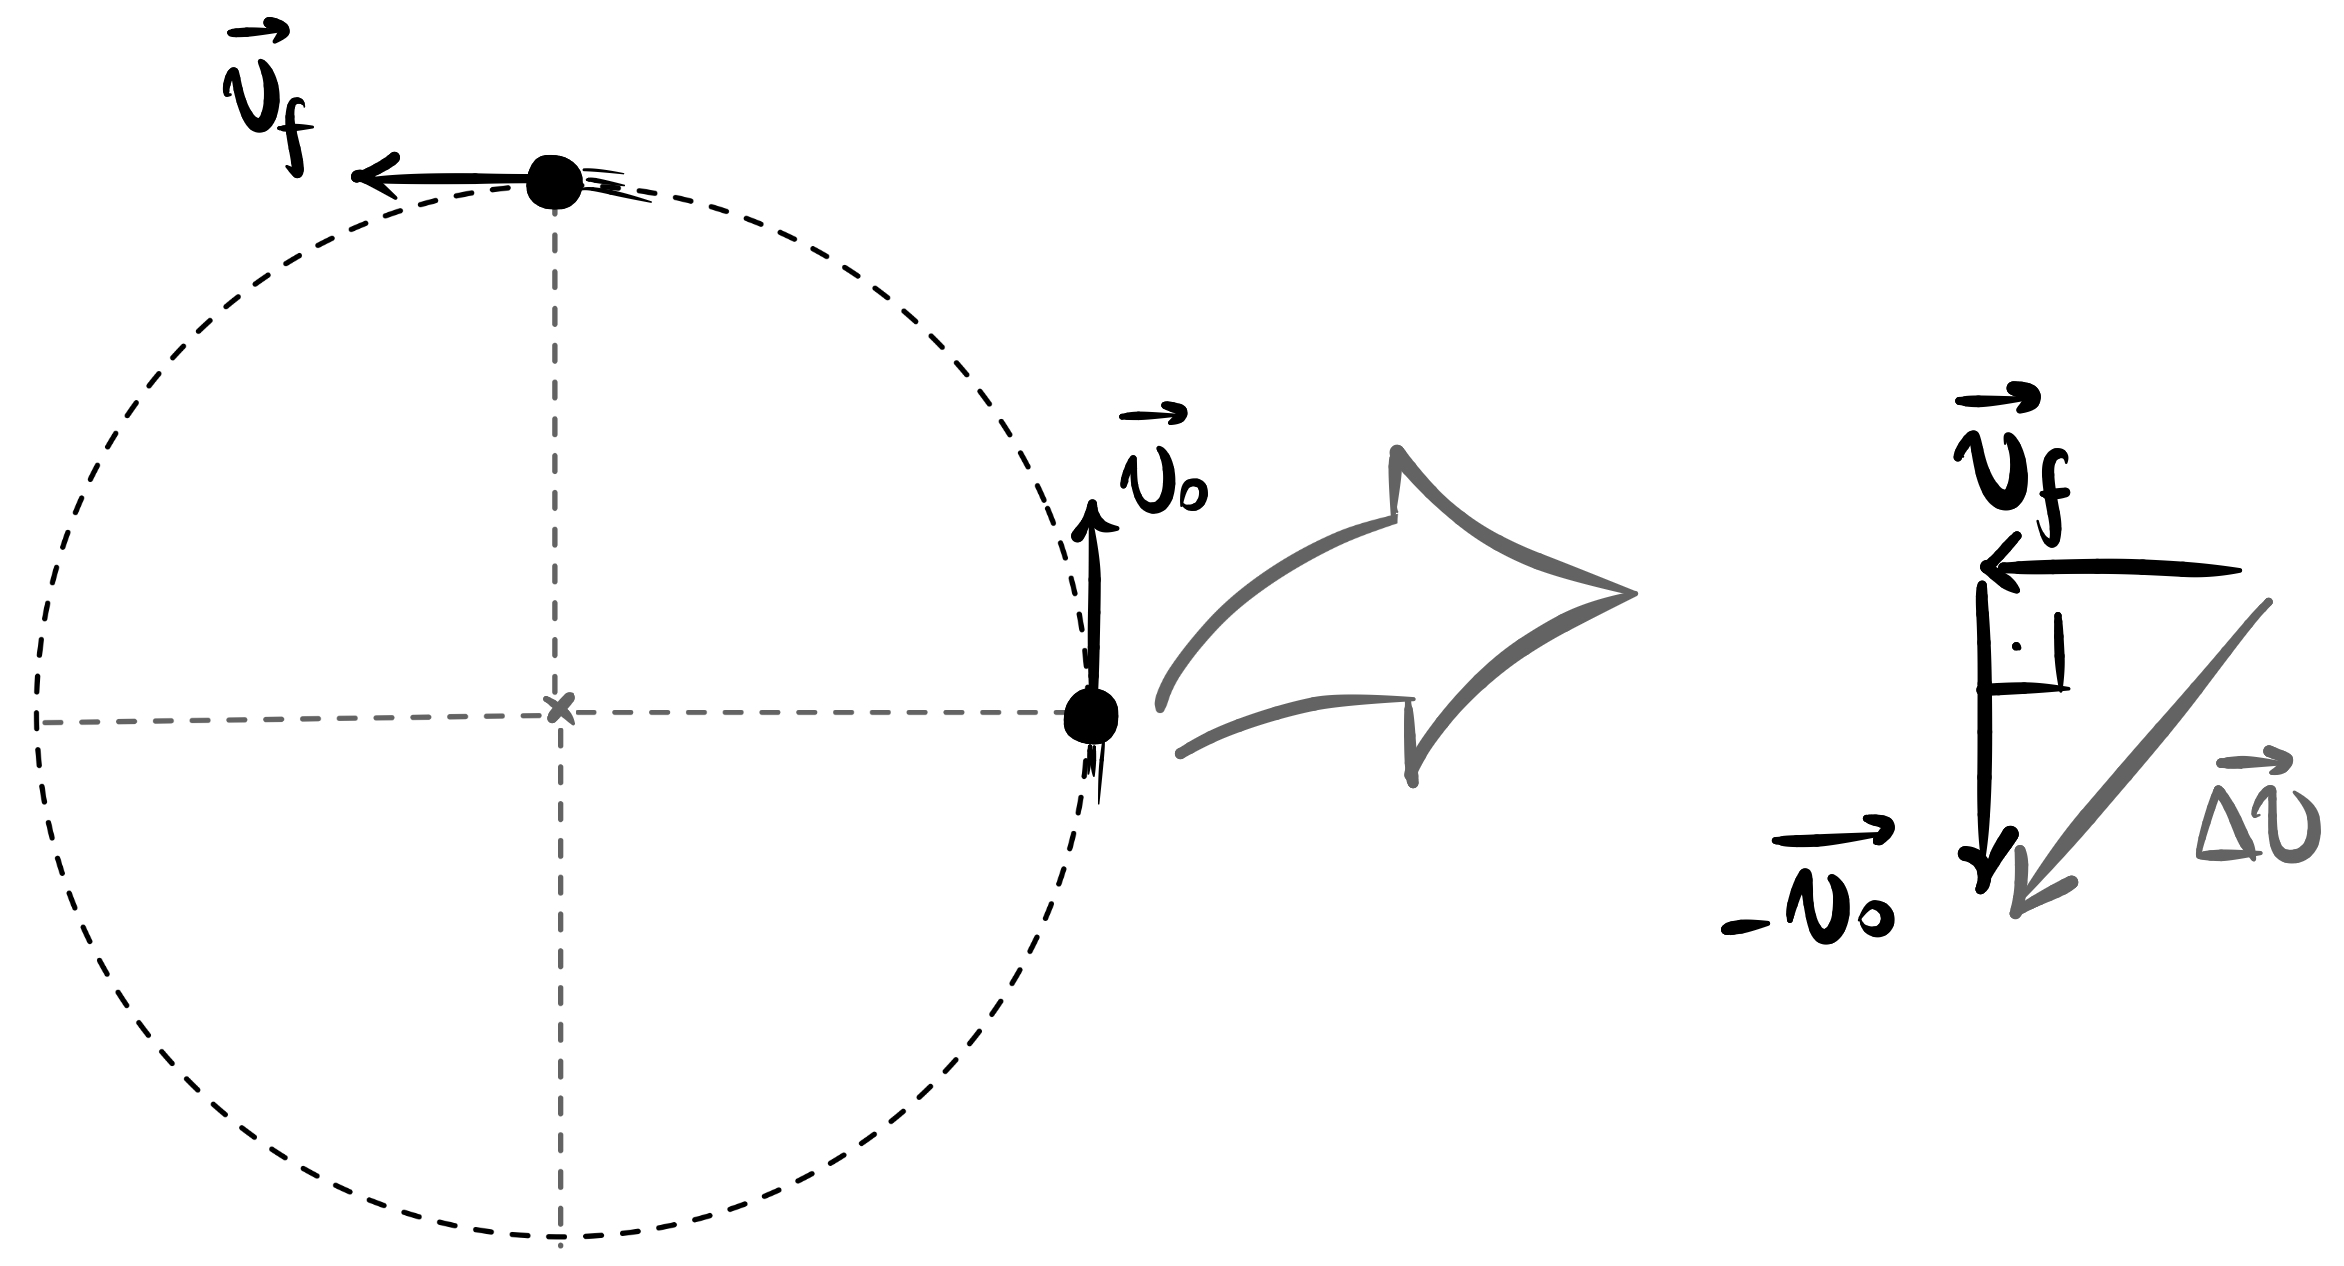
\includegraphics[width=0.6\linewidth]{imagenscinematicavetorial/fig_cinvet_aceleracaovetorialmediaexemplo0102.jpeg}
\captionof{figure}{}
\label{fig_cinvet_aceleracaovetorialmediaexemplo0102}
} 

Na parte direita da figura vemos o esboço do cálculo de $\Delta \vec{v}$, cujo módulo pode ser obtido pelo Teorema de Pitágoras:

$$ |\Delta \vec{v}|^2 = 10^2+10^2 \implies  |\Delta \vec{v}|=10\sqrt 2 \text{ m/s},$$

\noindent de modo que a aceleração vetorial média, neste intervalo, tem módulo

$$ | \vec{a}_m|= \dfrac{|\Delta \vec{v}|}{\Delta t}= \dfrac{10\sqrt 2 \text{ m/s}}{3\text{ s}} \implies \boxed{| \vec{a}_m|=\dfrac{10\sqrt2}{3}\text{ m/s$^2$}.}$$

 \item [(d)] O último intervalo de tempo é $\Delta t = t_2-t_1=5-3=2$s, de modo que a partícula terá completado $\sfrac{2}{12}=\sfrac{1}{6}$ de volta, o que significa ter girado $\sfrac{360^\circ}{6}=60^\circ$, situação ilustrada na Figura \ref{fig_cinvet_aceleracaovetorialmediaexemplo0103}.

{
\centering
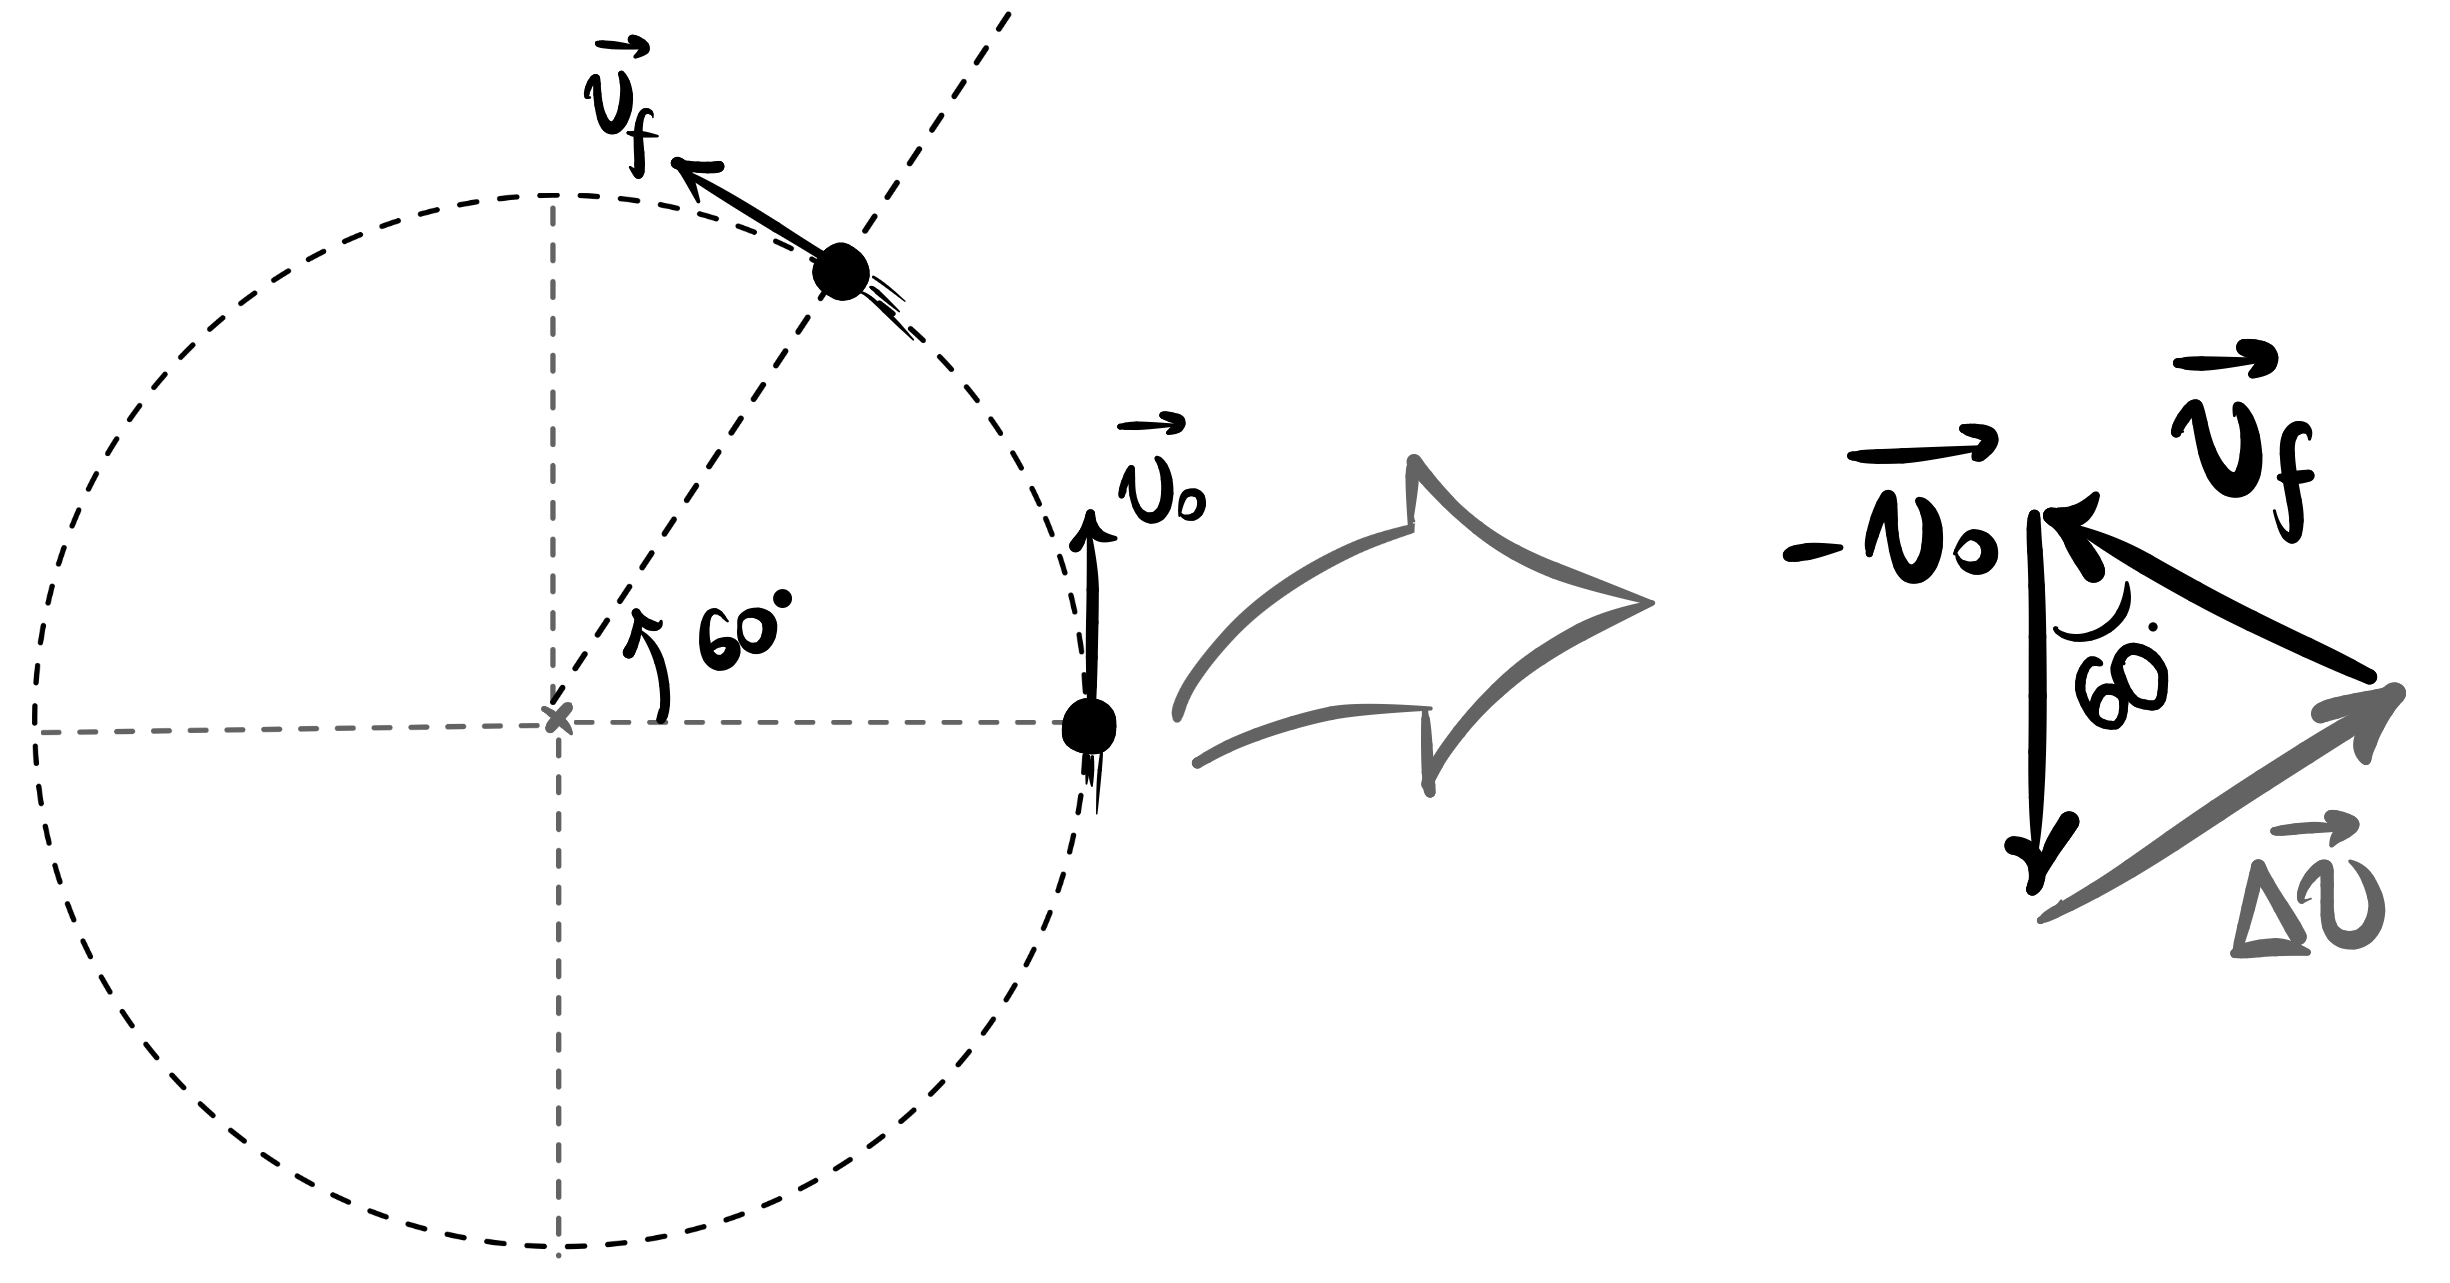
\includegraphics[width=0.6\linewidth]{imagenscinematicavetorial/fig_cinvet_aceleracaovetorialmediaexemplo0103.jpeg}
\captionof{figure}{}
\label{fig_cinvet_aceleracaovetorialmediaexemplo0103}
} 

Na parte direita da figura vemos o esboço do cálculo de $\Delta \vec{v}$, cujo módulo pode ser obtido observando que, em tal triângulo, os lados de tamanhos $|\vec{v}_0|$ e $|-\vec{v}_f|$ são iguais, de modo que os seus ângulos opostos também devem o ser -- o triângulo é isósceles. Como já temos $60^\circ$ para o ângulo de cima, cada ângulo da base precisa ter $\sfrac{(180^\circ-60^\circ)}{2}=60^\circ$, de modo que o triângulo é, na verdade, equilátero. 

Logo, temos que $|\Delta \vec{v}|=|\vec{v}_0|=|-\vec{v}_f|=10 \text{ m/s}$, de modo que a aceleração vetorial média, neste intervalo, tem módulo

$$ | \vec{a}_m|= \dfrac{|\Delta \vec{v}|}{\Delta t}= \dfrac{10 \text{ m/s}}{2\text{ s}} \implies \boxed{| \vec{a}_m|=5\text{ m/s$^2$}.}$$
     
     
    
\end{enumerate}

  
\end{exemplo}


\vspace{0.3cm}






\begin{exemplo}[Nível III]

Considere uma partícula que executa um movimento circular, de raio $R$, mantendo o módulo da sua velocidade sempre constante. Se a partícula leva um tempo $\tau$ para completar uma volta, mostre que o módulo da sua aceleração vetorial média entre os instantes $t=0s$ e $t$ é dado por

$$ |\vec{a}_m(t)|=\dfrac{4 \pi R}{t \tau}  \sin \left( \dfrac{\pi t}{\tau} \right).$$

\resolucao


Sendo a velocidade, em módulo, sempre constante, podemos computá-la por meio de $v=\sfrac{d}{t},$ e, para uma volta completa, teremos

$$ v=\dfrac{2 \pi R}{\tau}.$$

Seja $\theta$ o ângulo de giro para o intervalo de tempo $t$. Logo, tem-se 

$$ \dfrac{\theta}{t} = \dfrac{2 \pi}{\tau} \implies \theta = \dfrac{2 \pi t}{\tau}.$$

{
\centering
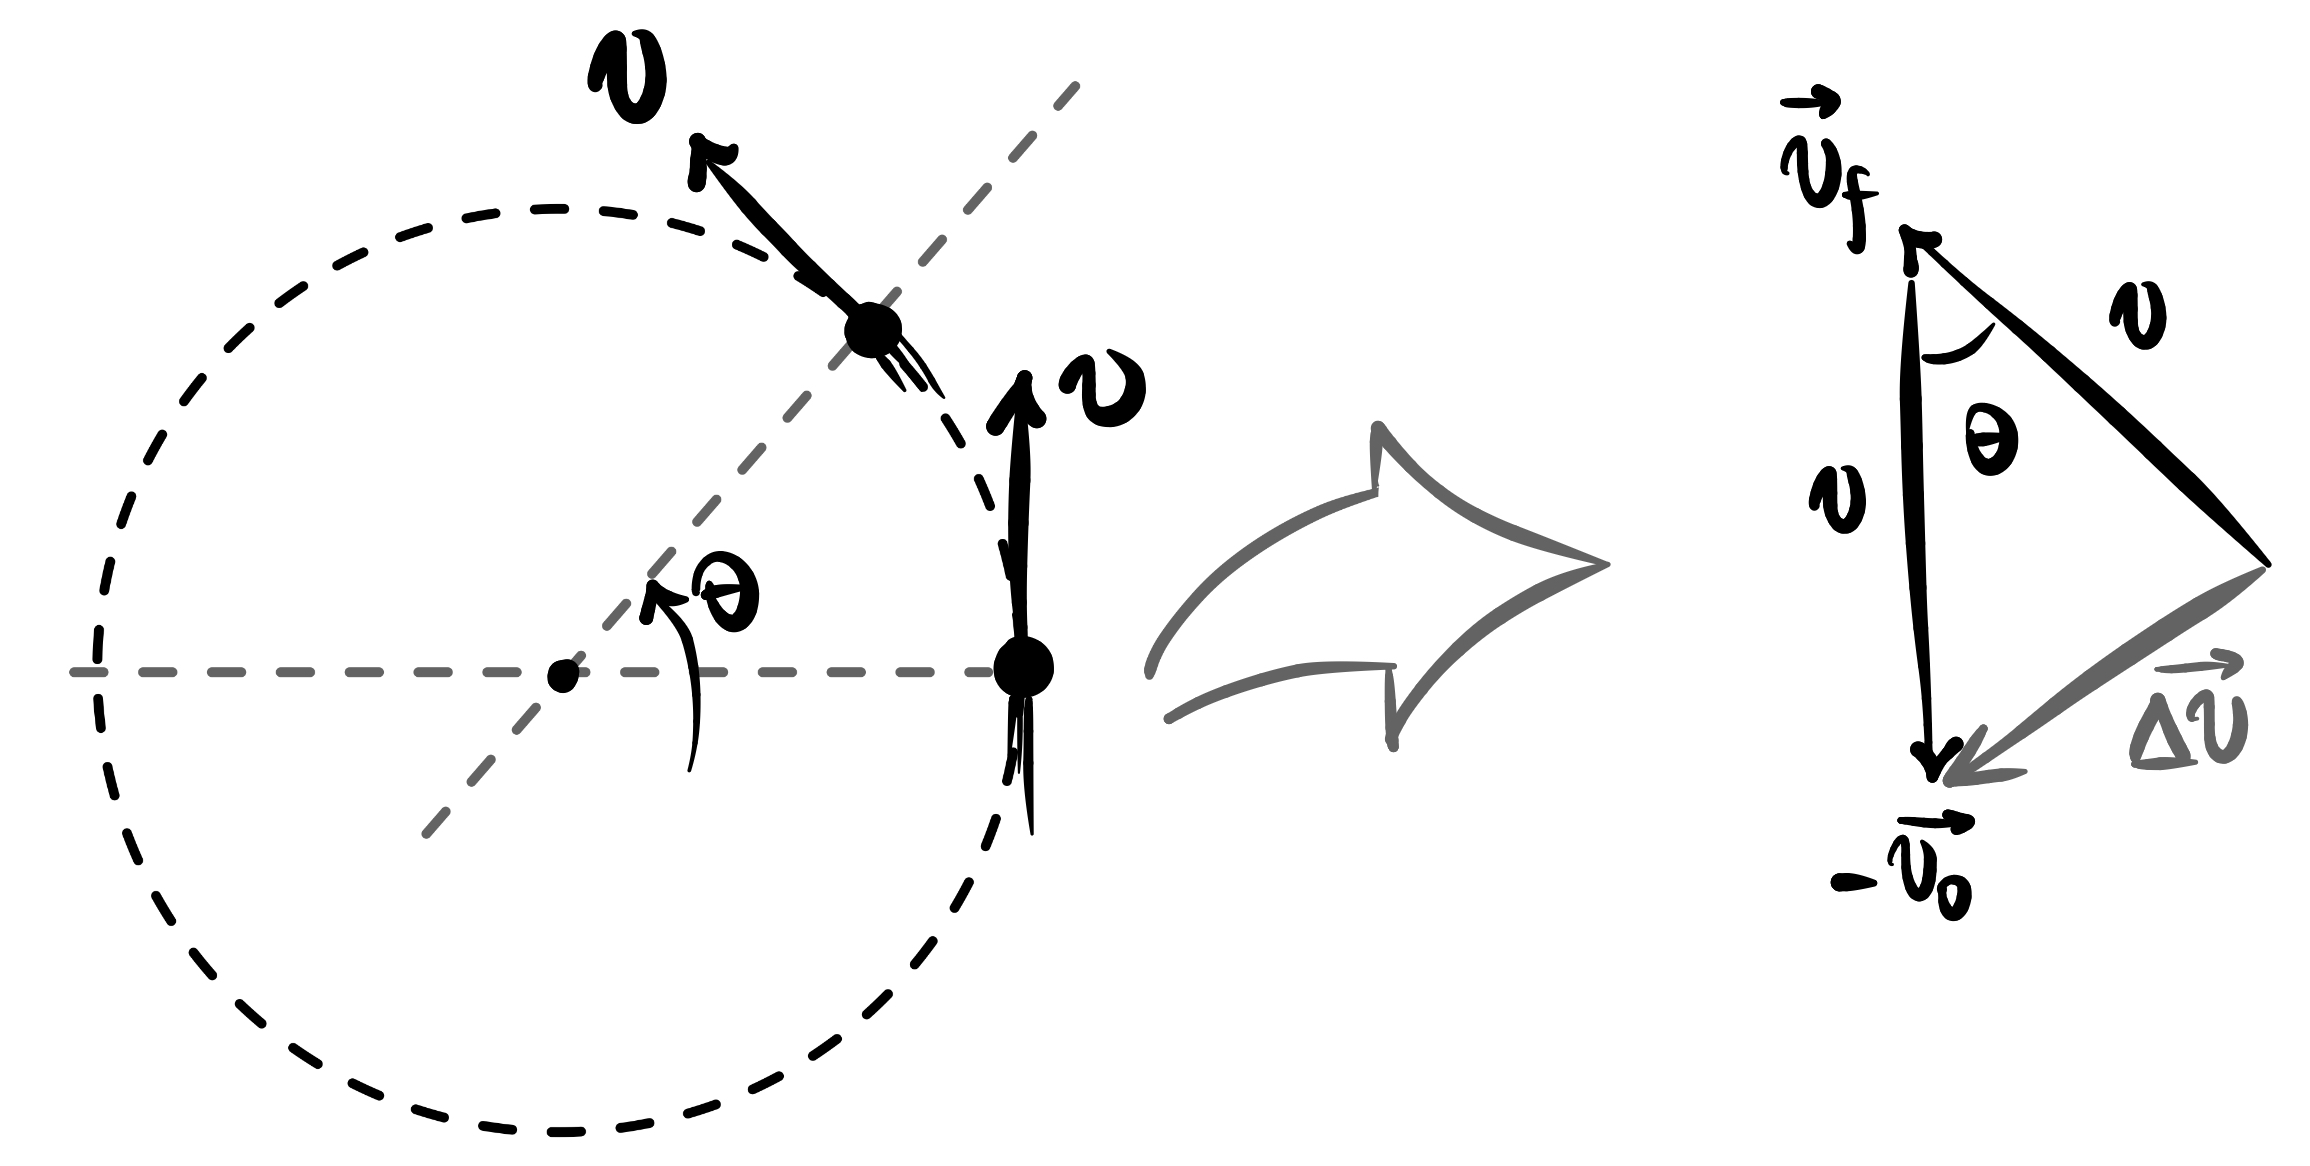
\includegraphics[width=0.5\linewidth]{imagenscinematicavetorial/fig_cinvet_aceleracaovetorialexemplonivel3.jpeg}
\captionof{figure}{}
\label{fig_cinvet_aceleracaovetorialexemplonivel3}
} 

A Figura \ref{fig_cinvet_aceleracaovetorialexemplonivel3} ilustra a situação e também o esboço dos vetores para o cálculo de $\Delta \vec{v}=\vec{v}_f-\vec{v}_0.$ Por meio da aplicação da Lei dos Cossenos no triângulo da figura, teremos:

 $$ |\Delta \vec{v}|^2= v^2+v^2 - 2 \cdot v \cdot v \cdot \cos \theta,$$

 \noindent que, por meio da fórmula do arco metade $\sin^2 \theta = \sfrac{(1-\cos \theta)}{2},$ nos leva a

 $$ |\Delta \vec{v}| = 2v \sin \left( \dfrac{\theta}{2} \right). $$



Assim, a aceleração vetorial média terá módulo, no intervalo de tempo $t$, dado por

$$ |\vec{a}_m| = \dfrac{ |\Delta \vec{v}|}{\Delta t} = \dfrac{ 2v \sin \left( \dfrac{\theta}{2} \right)}{t},$$

\noindent e, usando os valores de $\theta$ e $v$ calculados anteriormente em termos dos valores fornecidos, somos levados a

$$ \boxed{|\vec{a}_m(t)|=\dfrac{4 \pi R}{t \tau} \sin \left( \dfrac{\pi t}{\tau} \right),}$$

\noindent como queríamos demonstrar.\\

Sugerimos ao leitor que insira os valores de $t$ como sendo um período, meio período e um quarto de período para comparar os resultados com aqueles do exemplo anterior.

  
\end{exemplo}

\vspace{0.3cm}




\begin{secnivel}[Aceleração Centrípeta]{I}{Aceleração Centrípeta}
  
  \eqLdois{dem}{cinvet_eq_aceleracaocentripeta}{a_c=\dfrac{v^2}{r}}

\end{secnivel}








\secgfe{De onde vem}

Nos exemplos resolvidos da Equação \eqref{cinvet_eq_aceleracaovetorialmedia} ficou claro que, mesmo em um movimento no qual a velocidade não muda em valor, isto é, o tamanho do vetor é sempre constante, deve existir algum tipo de aceleração caso a direção desse vetor mude, ou seja, caso o movimento faça algum tipo de curva. O melhor movimento para avaliarmos isso é justamente aquele usado em tais exemplos: o Movimento Circular Uniforme (MCU).

O fato de ser um movimento uniforme implica que o valor (módulo) da velocidade do objeto é constante; logo, não existe a aceleração que até então conhecíamos: a aceleração que faz variar o valor da velocidade -- aceleração escalar. Contudo, no MCU, a direção do vetor velocidade muda o tempo inteiro, uma vez que este é sempre tangente à trajetória. Logo, deve haver aqui algum tipo de aceleração -- aquela responsável por alterar a direção do vetor velocidade, e não o seu módulo. À \textbf{componente} da aceleração que faz isso damos o nome de aceleração centrípeta, representada por $a_c.$

Logo, é como se a aceleração vetorial $\vec{a}$ fosse composta de duas partes, a aceleração centrípeta $\vec{a}_c$ e a aceleração tangencial $\vec{a}_t$. \footnote{Essa última é justamente a aceleração que faz variar o módulo da velocidade e coincide com o valor da conhecida aceleração escalar. Discutiremos tal componente em uma seção própria a ela.} Logo, a aceleração vetorial é

$$\boxed{ \vec{a} = \vec{a}_c + \vec{a}_t.}$$

Contudo, no MCU, como o valor da velocidade nunca muda, a aceleração $a_t$ será nula, logo

$$ \vec{a} = \vec{a}_c + \cancelto{0}{\vec{a}_t} \implies  \boxed{ \vec{a} = \vec{a}_c,}$$

\noindent ou seja, se calcularmos a aceleração vetorial usando a Equação \eqref{cinvet_eq_aceleracaovetorialmedia}, ela irá coincidir, no caso do MCU, com a aceleração centrípeta, que é quem queremos encontrar. Este será o caminho para construirmos a Equação \eqref{cinvet_eq_aceleracaocentripeta}. 

Considere, portanto, o MCU representado na Figura \ref{fig_cinvet_demonstracaoacentripeta01}, em que a circunferência tem raio $R$ e o valor da velocidade da partícula é $v$. Considere a partícula se movendo entre os pontos $A$ e $B,$ nos quais sua velocidade é dada pelos vetores $\vec{v}_1$ e $\vec{v}_2,$ respectivamente. Sendo o movimento uniforme, o módulo de tais vetores é o mesmo, isto é

$$ |\vec{v}_1| = |\vec{v}_2| = v.$$


{
\centering
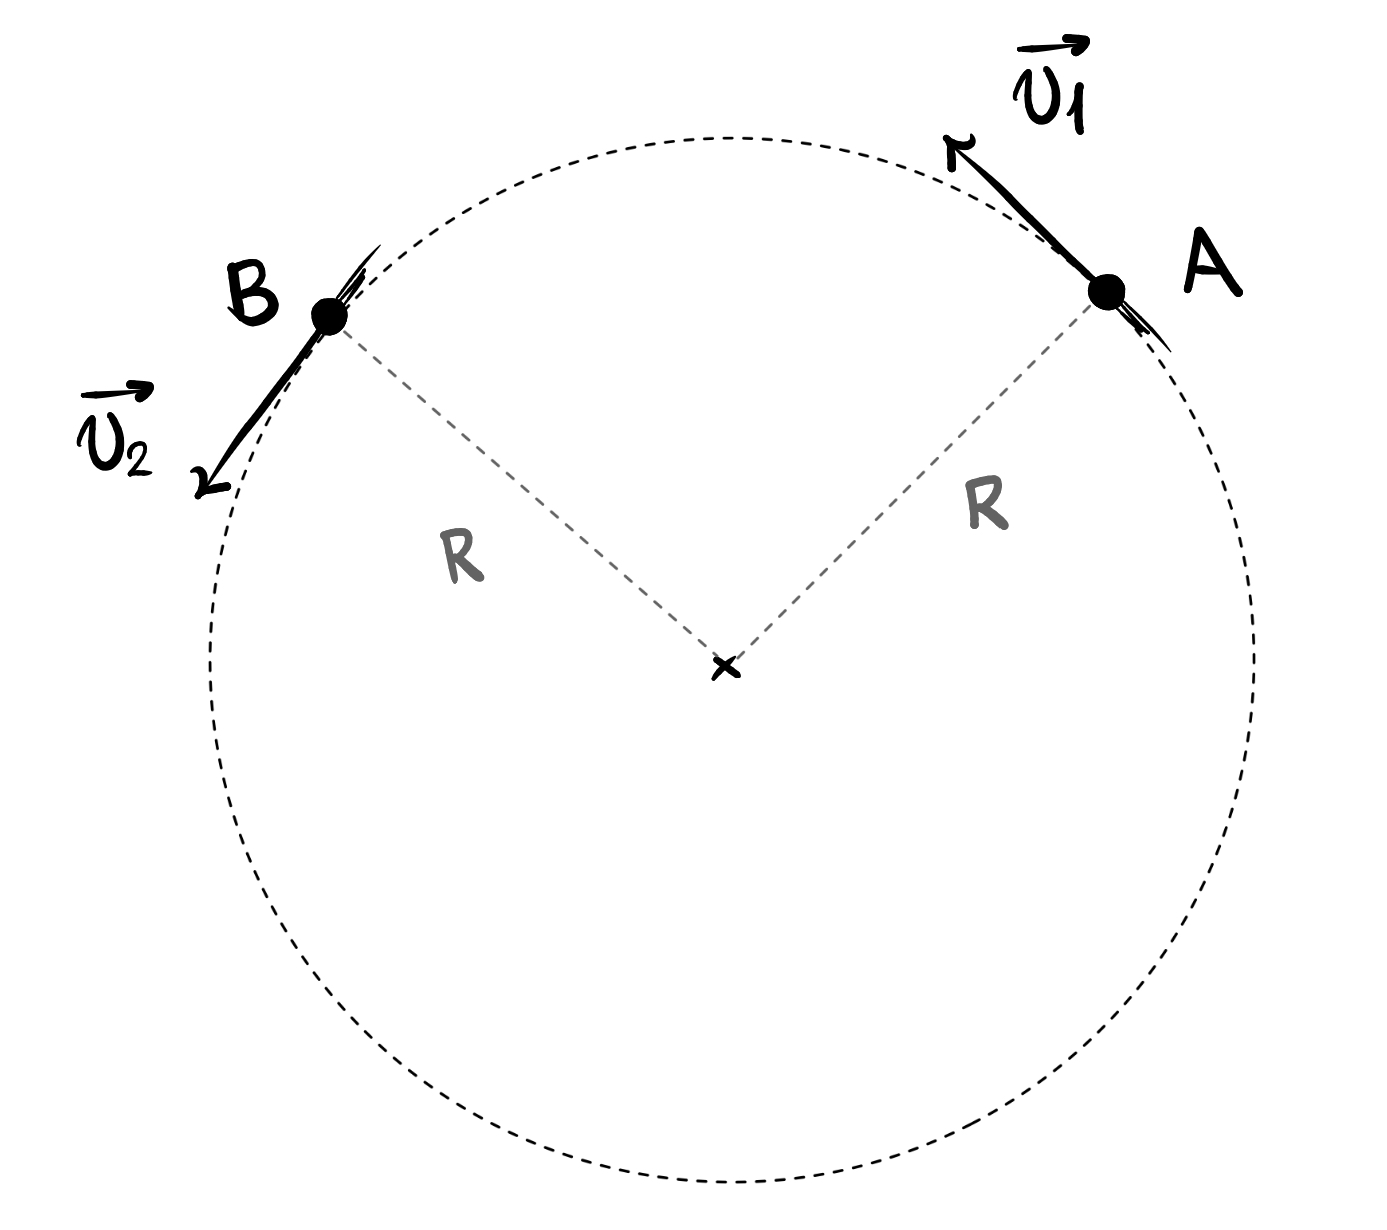
\includegraphics[width=0.35\linewidth]{imagenscinematicavetorial/demonstracaoacentripeta01.jpeg}
\captionof{figure}{Movimento Circular Uniforme: o módulo dos vetores $\vec{v}_1$ e $\vec{v}_2$ é o mesmo.}
\label{fig_cinvet_demonstracaoacentripeta01}
} 

\vspace{0.3cm}

Vimos que, neste caso, a aceleração centrípeta coincidirá com a aceleração vetorial, que é computada pela Equação \eqref{cinvet_eq_aceleracaovetorialmedia} por meio de:

$$ \vec{a} = \dfrac{\Delta \vec{v}}{\Delta t.}$$

A Figura \ref{fig_cinvet_demonstracaoacentripeta02} mostra o esboço do cálculo do vetor $\Delta \vec{v} = \vec{v}_2 -  \vec{v}_1 $. Na primeira imagem projetamos em linha pontilhada a direção dos dois vetores e os arrastamos, ao longo de tais linhas, de modo a desenhá-los com a origem de um deles coincidindo com a extremidade do outro. O vetor $\vec{v}_1$ teve seu sentido invertido para fazermos a soma $\Delta \vec{v} = \vec{v}_2 +  (-\vec{v}_1), $ que é um vetor que vai da origem do primeiro à extremidade do último, como a segunda imagem indica.


\vspace{0.3cm}
{
\centering
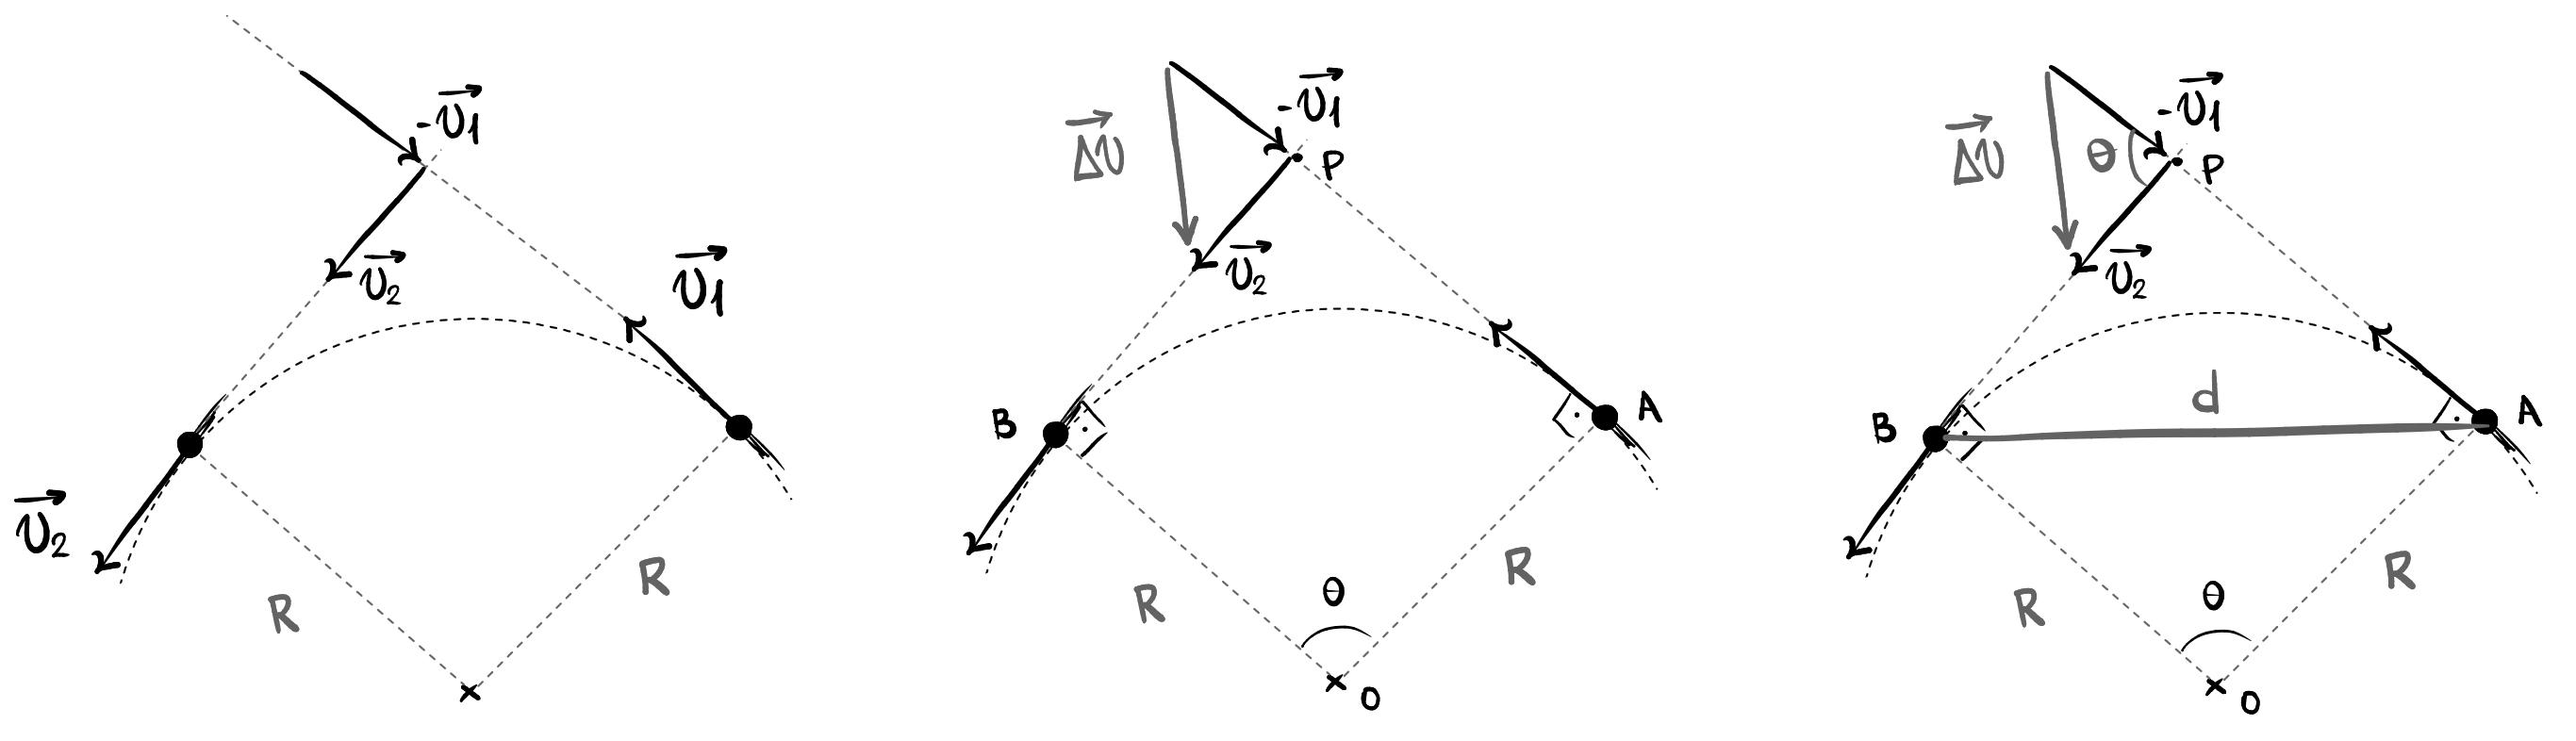
\includegraphics[width=1.0\linewidth]{imagenscinematicavetorial/demonstracaoacentripeta02.jpeg}
\captionof{figure}{Cálculo do vetor $\Delta \vec{v}$.}
\label{fig_cinvet_demonstracaoacentripeta02}
} 
\vspace{0.3cm}

Note, ainda na segunda imagem da Figura \ref{fig_cinvet_demonstracaoacentripeta02}, que os ângulos $\angle OAP$ e $\angle OBP$ são retos, haja vista que a velocidade é tangente à trajetória e, portanto, perpendicular ao raio. Logo, como os ângulos internos do quadrilátero $AOBP$ devem totalizar $360^\circ$, concluímos que o ângulo $\angle APB$ deve medir $180^\circ - \theta,$ de onde obtemos que o ângulo adjacente à ele, que é seu suplementar -- o ângulo entre os vetores $\vec{v}_2$ e $-\vec{v}_1$ -- terá medida igual a $\theta$, como mostra a terceira imagem da figura. Dessa terceira imagem extrairemos os triângulos $AOB$ e o triângulo formado pelos vetores, que se encontram na Figura \ref{fig_cinvet_demonstracaoacentripeta03}.

\vspace{0.3cm}

{
\centering
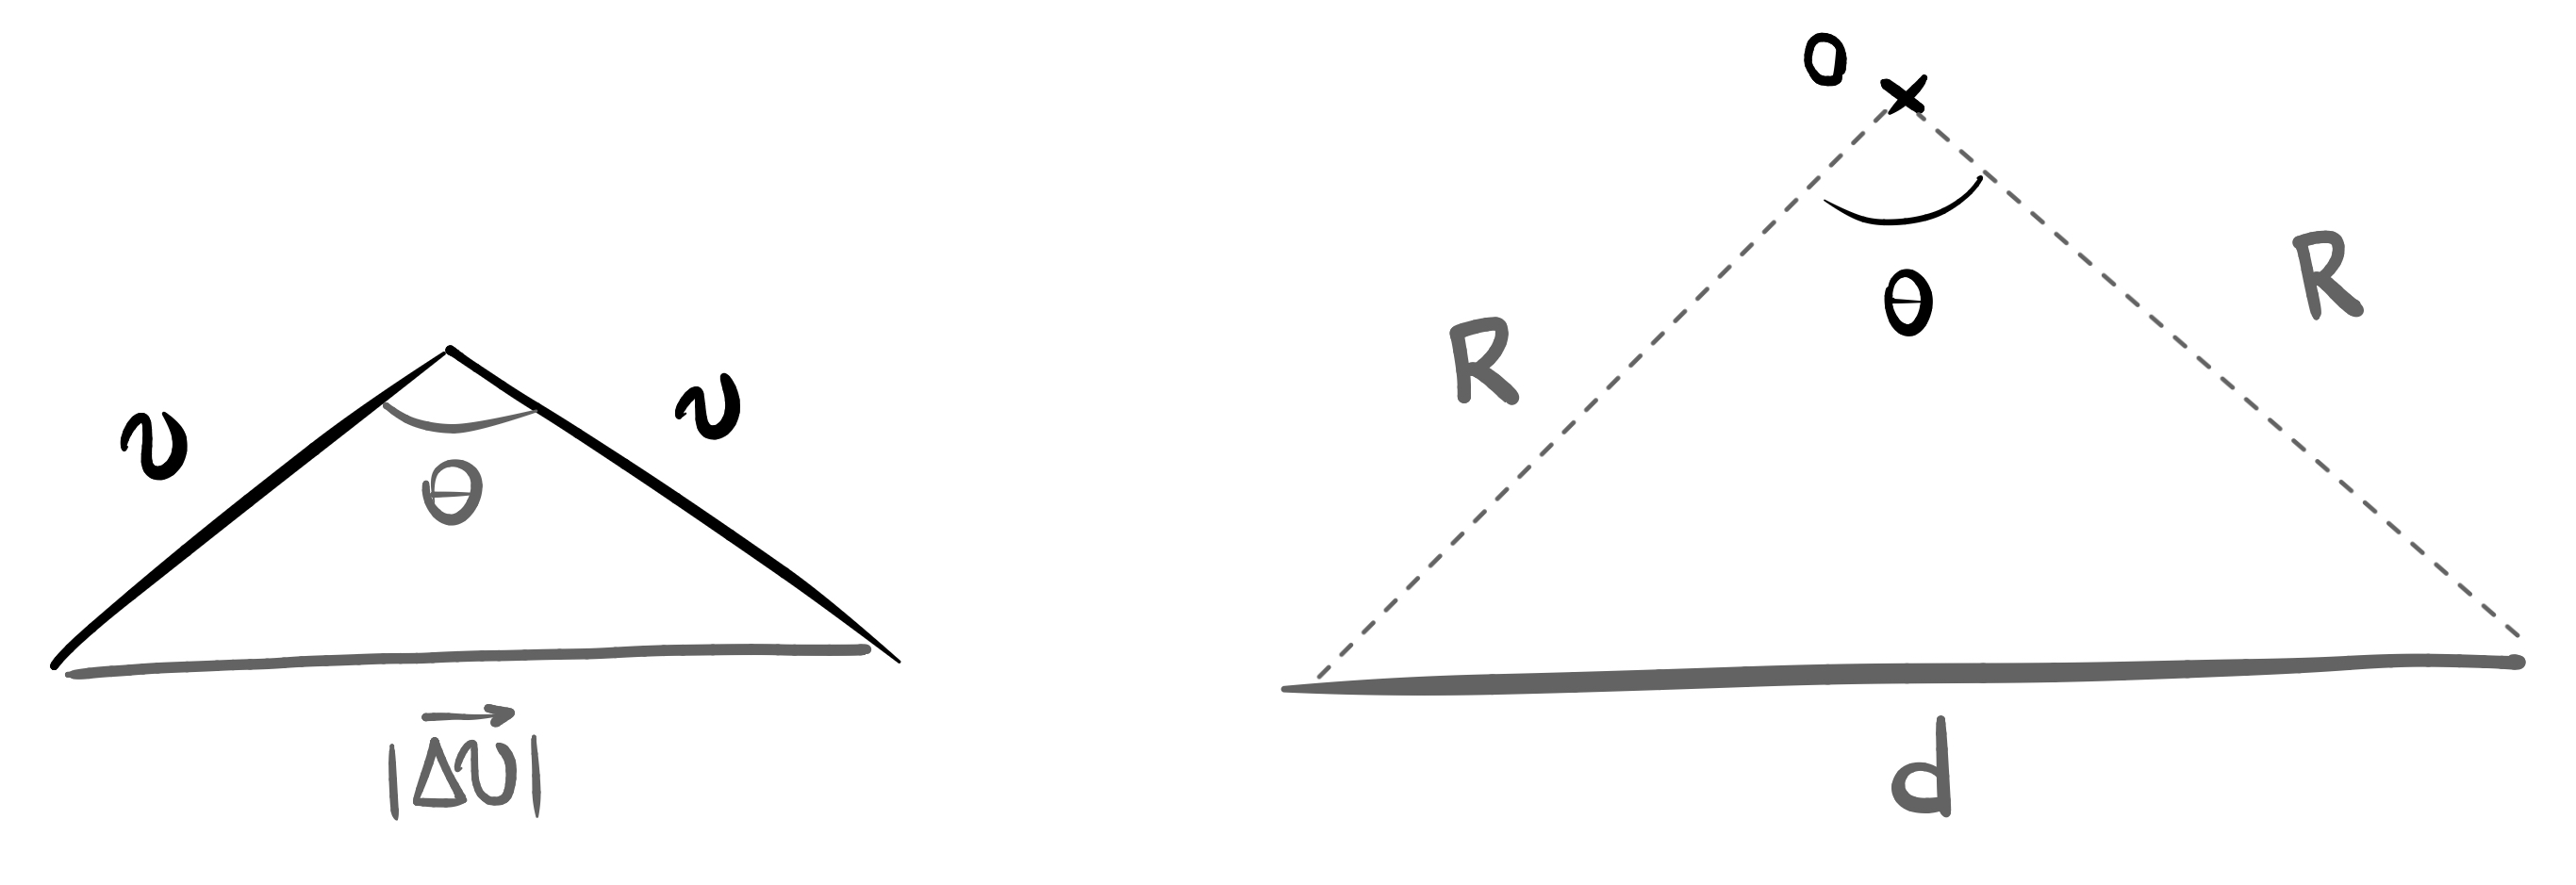
\includegraphics[width=0.6\linewidth]{imagenscinematicavetorial/demonstracaoacentripeta03.jpeg}
\captionof{figure}{O triângulo dos vetores é semelhante ao triângulo geométrico formado pelos raios e pela distância.}
\label{fig_cinvet_demonstracaoacentripeta03}
} 
\vspace{0.3cm}

Note que esses triângulos são semelhantes: ambos possuem o ângulo $\theta$ e, como os dois são isósceles, os ângulos da base também serão iguais. Logo, por semelhança de triângulos, podemos escrever que

$$ \dfrac{|\Delta \vec{v}|}{d} = \dfrac{v}{R} \implies |\Delta \vec{v}| = \dfrac{vd}{R},$$

\noindent mas, sendo o movimento uniforme, podemos escrever que $d=v\Delta t,$ de modo que somos levados a

$$ |\Delta \vec{v}| = \dfrac{v}{R} \cdot v\Delta t\implies \boxed{\dfrac{|\Delta \vec{v}|}{\Delta t} = \dfrac{v^2}{R}.} $$


Perceba que, pela definição da Equação \eqref{cinvet_eq_aceleracaovetorialmedia}, o que calculamos acima é justamente o módulo do vetor aceleração. Mas, como vimos, no MCU só existe um tipo de aceleração: a aceleração responsável por mudar a direção do vetor velocidade, ou seja, a aceleração centrípeta. Assim, temos que, para o MCU,

$$ |\vec{a}| = a_c = \dfrac{v^2}{R},$$

\noindent como queríamos demonstrar.

Sobre tal equação é importante pontuar algumas observações:

\begin{enumerate}
    \item [(i)] A Equação \eqref{cinvet_eq_aceleracaocentripeta} vale para qualquer tipo de movimento curvilíneo. Demonstramos ela nessa seção partindo do MCU para fins didáticos, uma vez que este é o movimento no qual só há aceleração centrípeta, simplificando os cálculos e a geometria.

    Para qualquer tipo de movimento que faça curva, portanto, existirá uma aceleração, calculada pela Equação \eqref{cinvet_eq_aceleracaocentripeta}, que é responsável por fazer a mudança na direção do vetor velocidade e, portanto, possibilitar que o movimento seja curvo.

    Para o leitor curioso que pode ter se indagado a respeito do que significaria o raio $R$ na Equação \eqref{cinvet_eq_aceleracaocentripeta} no caso de um movimento que não seja circular, trataremos disso nas próximas linhas. Adianto ao nobre leitor que a discussão que se segue é um pouco mais abstrata -- de modo que pode ser pulada em uma primeira leitura.


A resposta começa com uma observação simples: olhe com atenção para
qualquer curva e, num determinado ponto $P$, tente encontrar o círculo
que melhor a ``\emph{abraça}'' naquele instante — aquele que toca a curva em
$P$ e se curva com a mesma
intensidade. Esse círculo especial é chamado de \textit{círculo
osculador} (do latim \textit{osculari}, ``beijar''), e seu raio recebe
o nome de \textit{raio de curvatura} da trajetória naquele ponto.

\vspace{0.3cm}
{
\centering
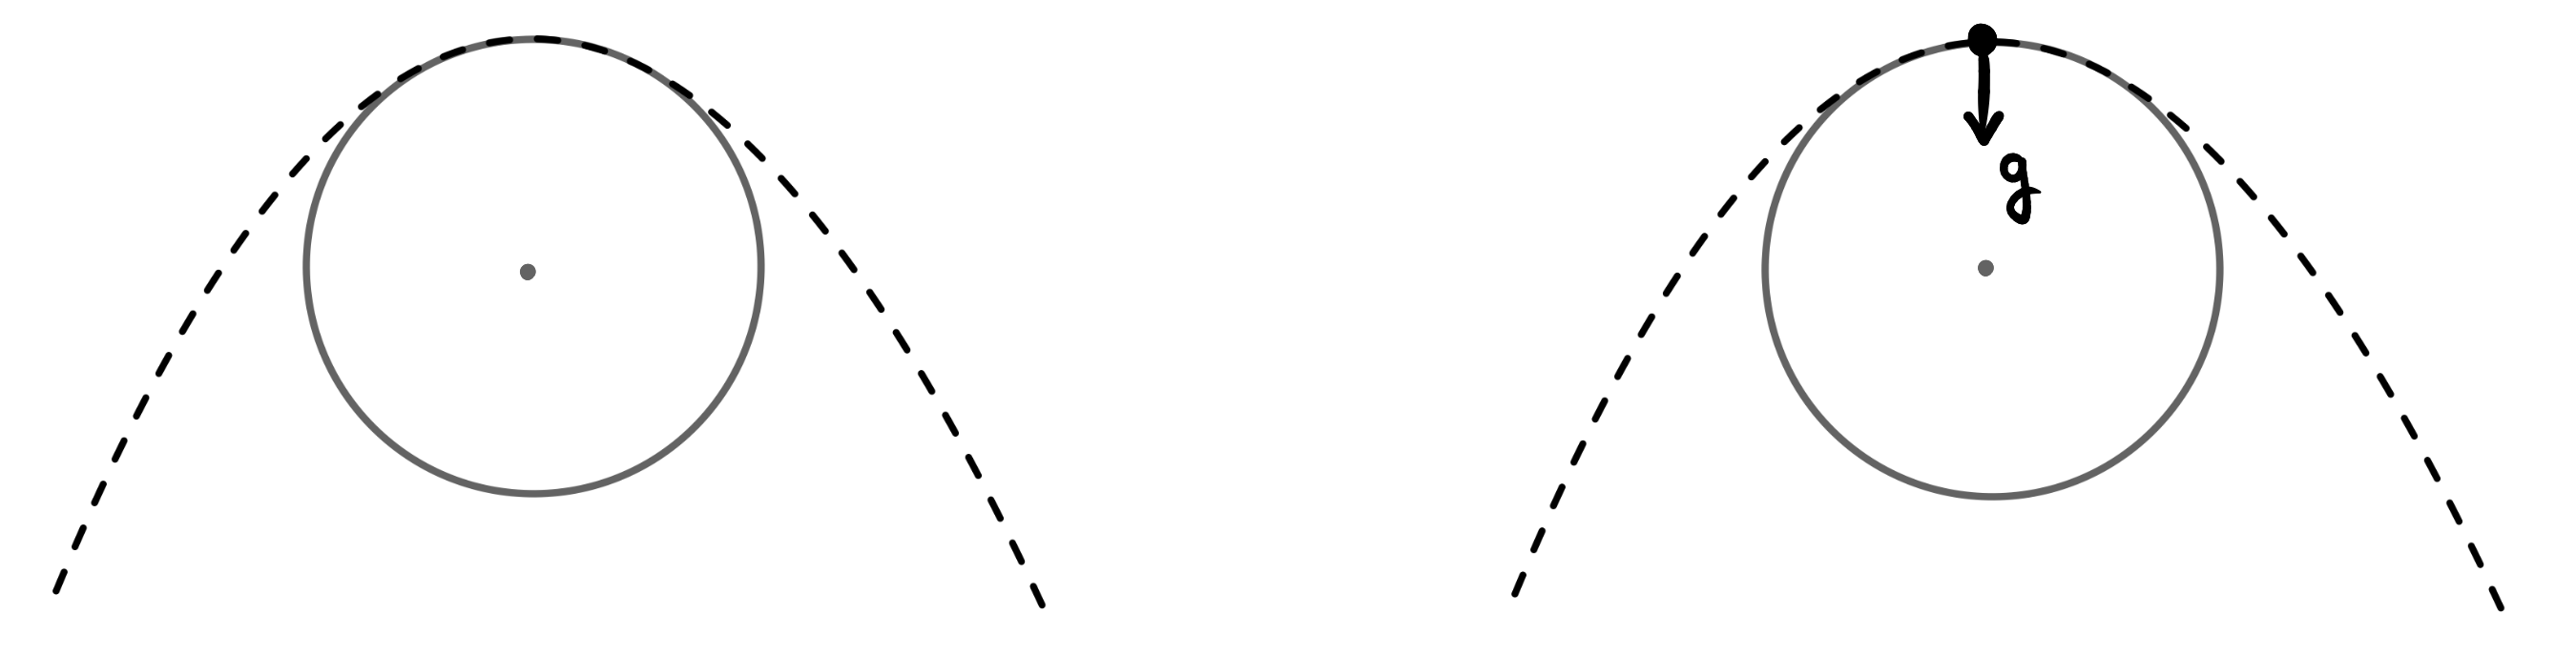
\includegraphics[width=0.75\linewidth]{imagenscinematicavetorial/circunferenciaoscular.png}
\captionof{figure}{A circunferência oscular.}
\label{fig_cinvet_circoscular}
} 
\vspace{0.3cm}

A Figura \ref{fig_cinvet_circoscular} ilustra a ideia. No ponto $P$, o círculo tracejado e a
trajetória se tocam tão intimamente que, visto de perto, seria
impossível distingui-los — eles compartilham a mesma tangente e a
mesma curvatura. Um pouco além de $P$, porém, os dois caminhos se
dividem: a trajetória segue o seu curso, e o círculo segue o seu.

O que torna isso poderoso é que a Equação \eqref{cinvet_eq_aceleracaocentripeta} continua válida em
qualquer ponto de qualquer trajetória curva, desde que $R$ seja
interpretado como esse raio de curvatura local:
%
\begin{equation}
    a_c = \frac{v^2}{R}.
    \nonumber
\end{equation}
%
Quando a curva é muito fechada, o círculo osculador é pequeno, $R$ é
pequeno, e a aceleração centrípeta necessária é grande. Quando a
trajetória é quase reta, o círculo osculador é enorme — no limite, uma
linha reta corresponde a um círculo de raio infinito —, e $a_c \to 0$.

Considere, por exemplo, no topo da parábola, como a
segunda imagem da Figura \ref{fig_cinvet_circoscular} ilustra. Naquele instante, a velocidade é puramente
horizontal e a única aceleração que age sobre o projétil é a gravidade
$g$, apontando verticalmente para baixo — exatamente em direção ao
centro $C$ do círculo osculador. A gravidade, portanto, desempenha o
papel de aceleração centrípeta, e isso é suficiente para determinar o
raio de curvatura da parábola naquele ponto.




    

    \item [(ii)] O leitor mais atento pode ter se sentido desconfortável quando usamos que o segmento de tamanho $d$, na terceira imagem da Figura \ref{fig_cinvet_demonstracaoacentripeta02}, fosse igual à distância percorrida pela partícula. A distância $d$, na verdade, é igual ao comprimento do arco pontilhado de circunferência -- essa é a trajetória que o corpo percorre. Já a distância em linha reta entre os pontos $A$ e $B$ é o deslocamento, que, em geral, é diferente da distância. Contudo, como mostra a Figura \ref{fig_cinvet_demonstracaoacentripeta04}, para intervalos de tempo muito pequenos a distância percorrida -- a linha pontilhada -- fica cada vez mais próxima do deslocamento -- linha cheia -- de modo que essas duas grandezas coincidem se o tempo for suficientemente pequeno, como discutimos na construção da Equação \eqref{cinvet_eq_velocidadevetorialmedia}.

\vspace{0.3cm}
{
\centering
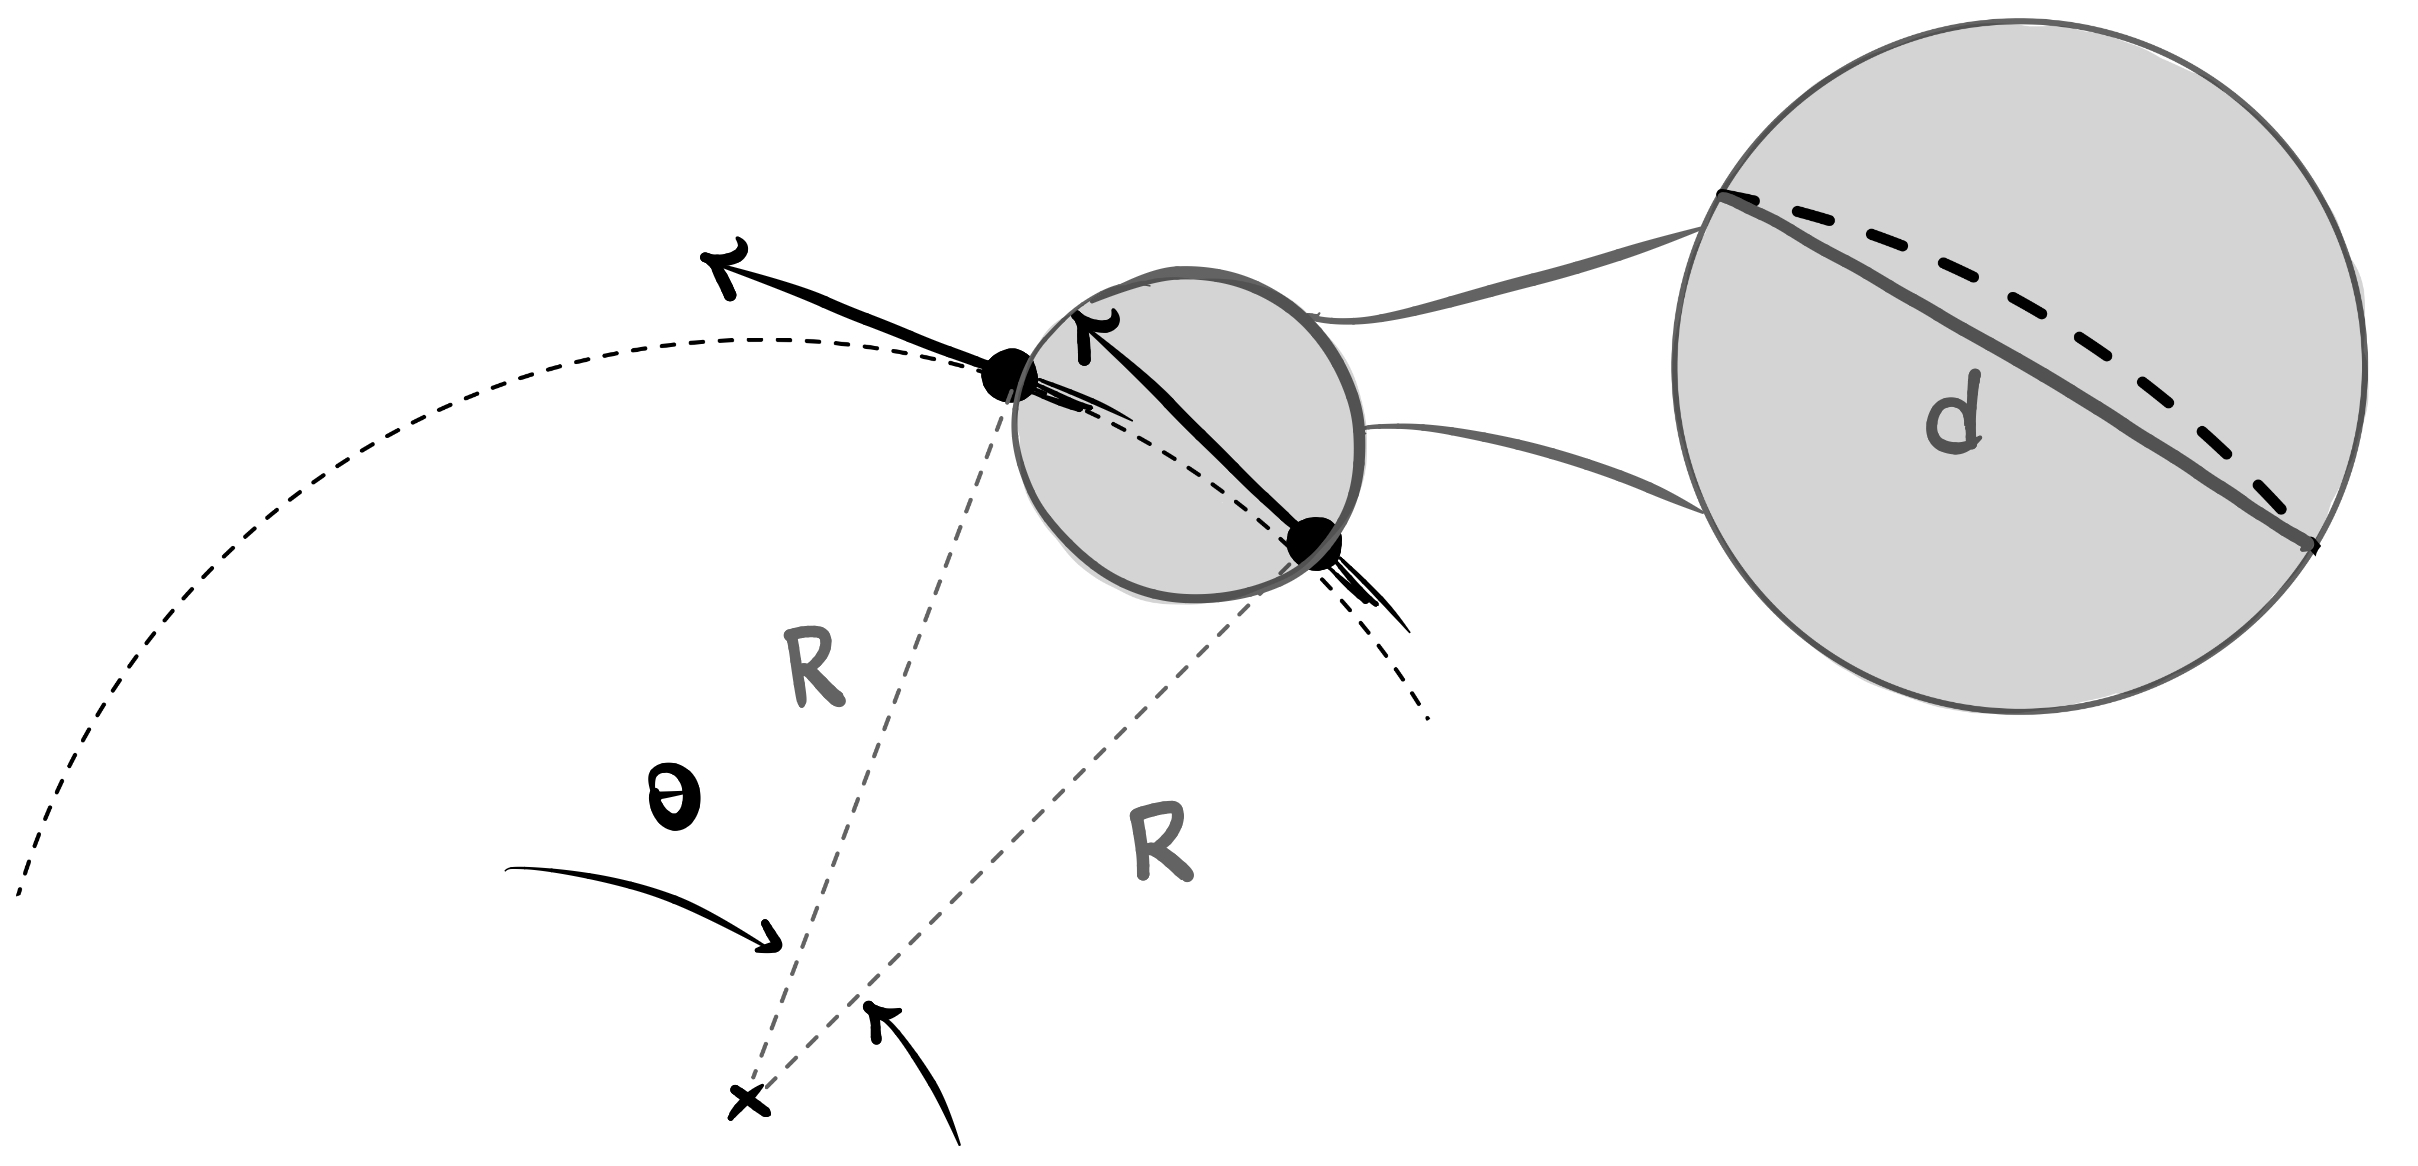
\includegraphics[width=0.6\linewidth]{imagenscinematicavetorial/demonstracaoacentripeta04.jpeg}
\captionof{figure}{O deslocamento e a distância percorrida coincidem quando o intervalo de tempo é muito pequeno.}
\label{fig_cinvet_demonstracaoacentripeta04}
} 
\vspace{0.3cm}

Como queremos calcular a aceleração vetorial em um ponto específico da trajetória do corpo, a ideia é calcular a aceleração vetorial média, porém usando um intervalo de tempo tão pequeno que, como quase não deu tempo da partícula se mover, estaremos praticamente calculando a aceleração naquele instante. 

      \item [(iii)]  Com base na ideia anterior, como vamos avaliar um intervalo de tempo muito curto para obter a aceleração da partícula em um instante específico -- e não uma média entre dois instantes distantes -- o ângulo de abertura $\theta$ dos triângulos da Figura \ref{fig_cinvet_demonstracaoacentripeta03} será muito pequeno. A própria Figura \ref{fig_cinvet_demonstracaoacentripeta04} já evidencia isso: em um intervalo de tempo curto a partícula se move muito pouco, de modo que a abertura angular $\theta$ é pequena. 

      Na verdade a abertura angular é tão pequena, mas tão pequena, que o ângulo $\theta$ é praticamente zero, como mostra a Figura \ref{fig_cinvet_acentripetaapontaparacentro1}. No caso limite, como a última imagem tenta mostrar, os ângulos da base do triângulo isósceles tendem a $90^\circ.$ Para que isso fique claro, sendo $\alpha$ o valor de cada ângulo, precisamos que 
       
       $$ \alpha + \alpha + \theta = 180^\circ,$$

       \noindent contudo, sendo $\theta$ praticamente zero, vemos que
       
  $$ \alpha + \alpha + \cancelto{0}{\theta} = 180^\circ \implies  \boxed{\alpha =90^\circ.}$$
  
\vspace{0.3cm}
{
\centering
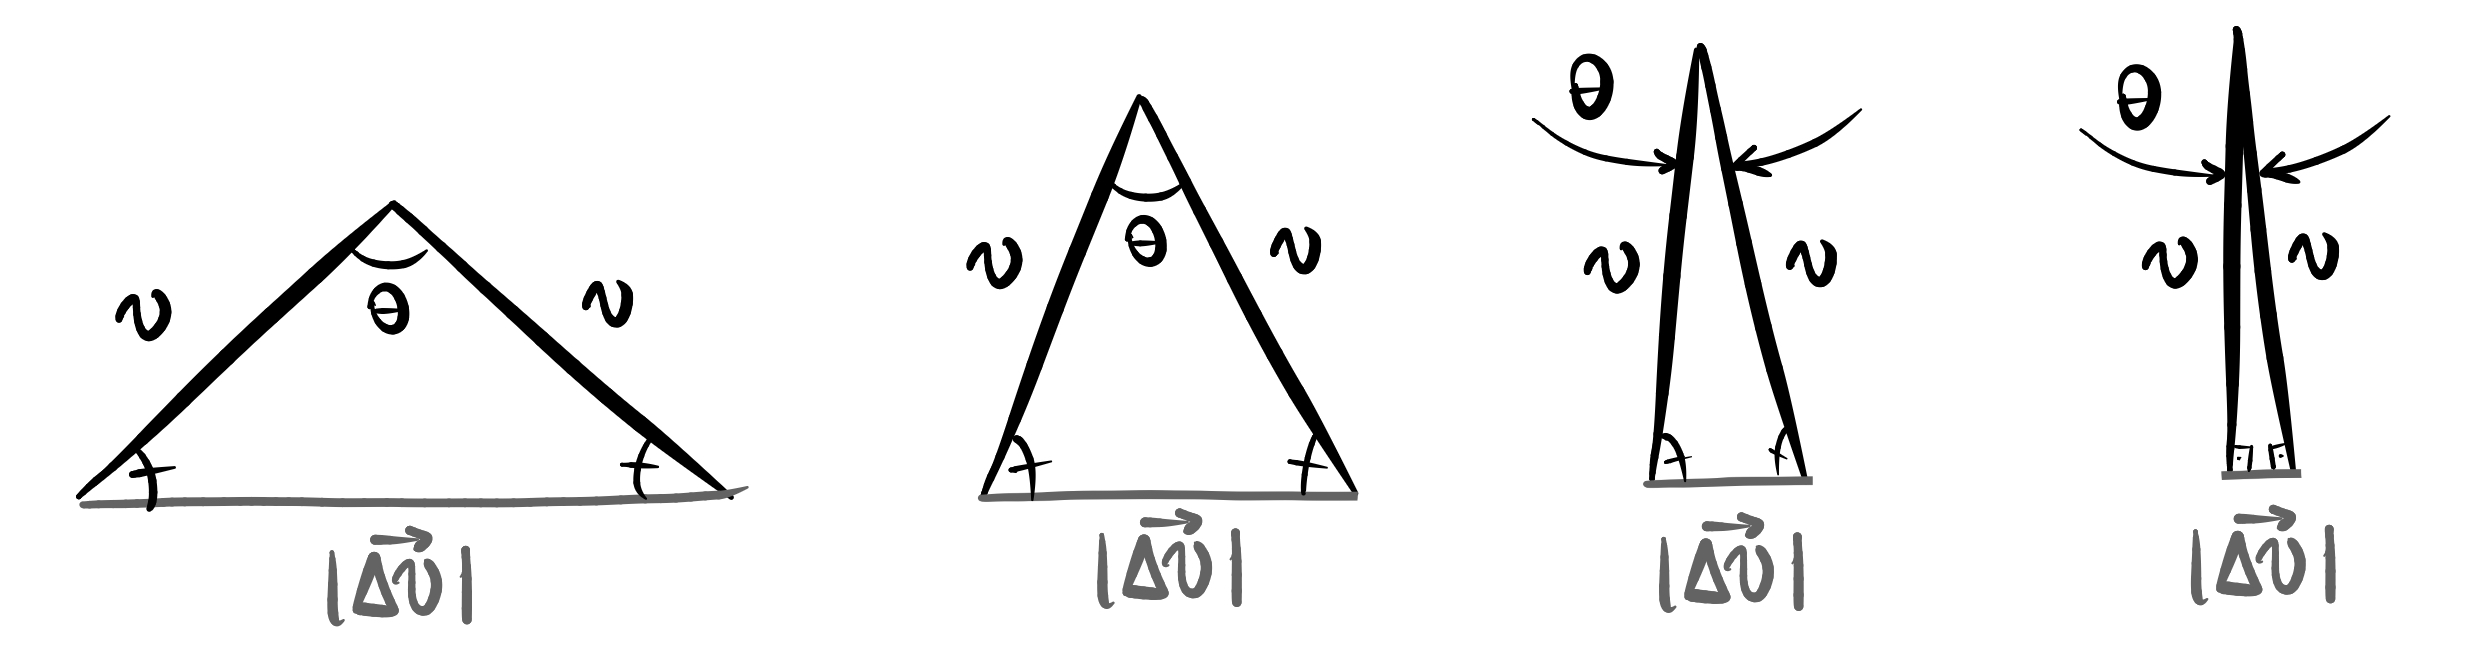
\includegraphics[width=0.8\linewidth]{imagenscinematicavetorial/acentripetaapontaparacentro1.jpeg}
\captionof{figure}{Quando o intervalo de tempo é muito curto a abertura angular é muito pequena, de modo que os ângulos iguais do triângulo tendem a $90^\circ$ cada.}
\label{fig_cinvet_acentripetaapontaparacentro1}
} 
\vspace{0.3cm}

Contudo, lembre-se que triângulos da Figura \ref{fig_cinvet_acentripetaapontaparacentro1} representam, na verdade, o triângulo dos vetores $-\vec{v}_1$, $\vec{v}_2$ e $\Delta \vec{v}$ da terceira imagem da Figura \ref{fig_cinvet_demonstracaoacentripeta02}. Ou seja, o ângulo $\alpha$ em questão é o ângulo entre o vetor $\Delta \vec{v}$ e o vetor velocidade da partícula (seja ele $\vec{v}_1$ ou $\vec{v}_2$, porque, como o intervalo de tempo é curto, tais vetores serão praticamente paralelos -- quase não deu tempo da velocidade mudar de direção). 

Estamos concluindo, portanto, que o vetor $\Delta \vec{v}$ é perpendicular à velocidade da partícula. Porém, sendo a aceleração vetorial dada por

$$ \vec{a} = \dfrac{\Delta \vec{v}}{\Delta t},$$

\noindent vê-se que os vetores $\vec{a}$ e ${\Delta \vec{v}}$ possuem a mesma direção e o mesmo sentido, uma vez que são múltiplos escalares um do outro (sendo tal escalar -- um intervalo de tempo -- positivo). Logo, sendo a aceleração vetorial neste contexto puramente centrípeta, a conclusão final é que

$$ \boxed{\text{ a aceleração centrípeta é perpendicular ao vetor velocidade em cada instante.}}$$

Sendo a velocidade sempre tangente à trajetória, a direção perpendicular à tangente em uma circunferência é a direção radial (direção dos raios da circunferência), de forma que a conclusão acima está dizendo que a aceleração centrípeta, portanto, sempre aponta na direção do centro da circunferência -- chamada de direção centrípeta ou direção radial. Por isso, inclusive, ela leva esse nome. A Figura \ref{fig_cinvet_acentripetaapontaparacentro2} ilustra este fato.


\vspace{0.3cm}
{
\centering
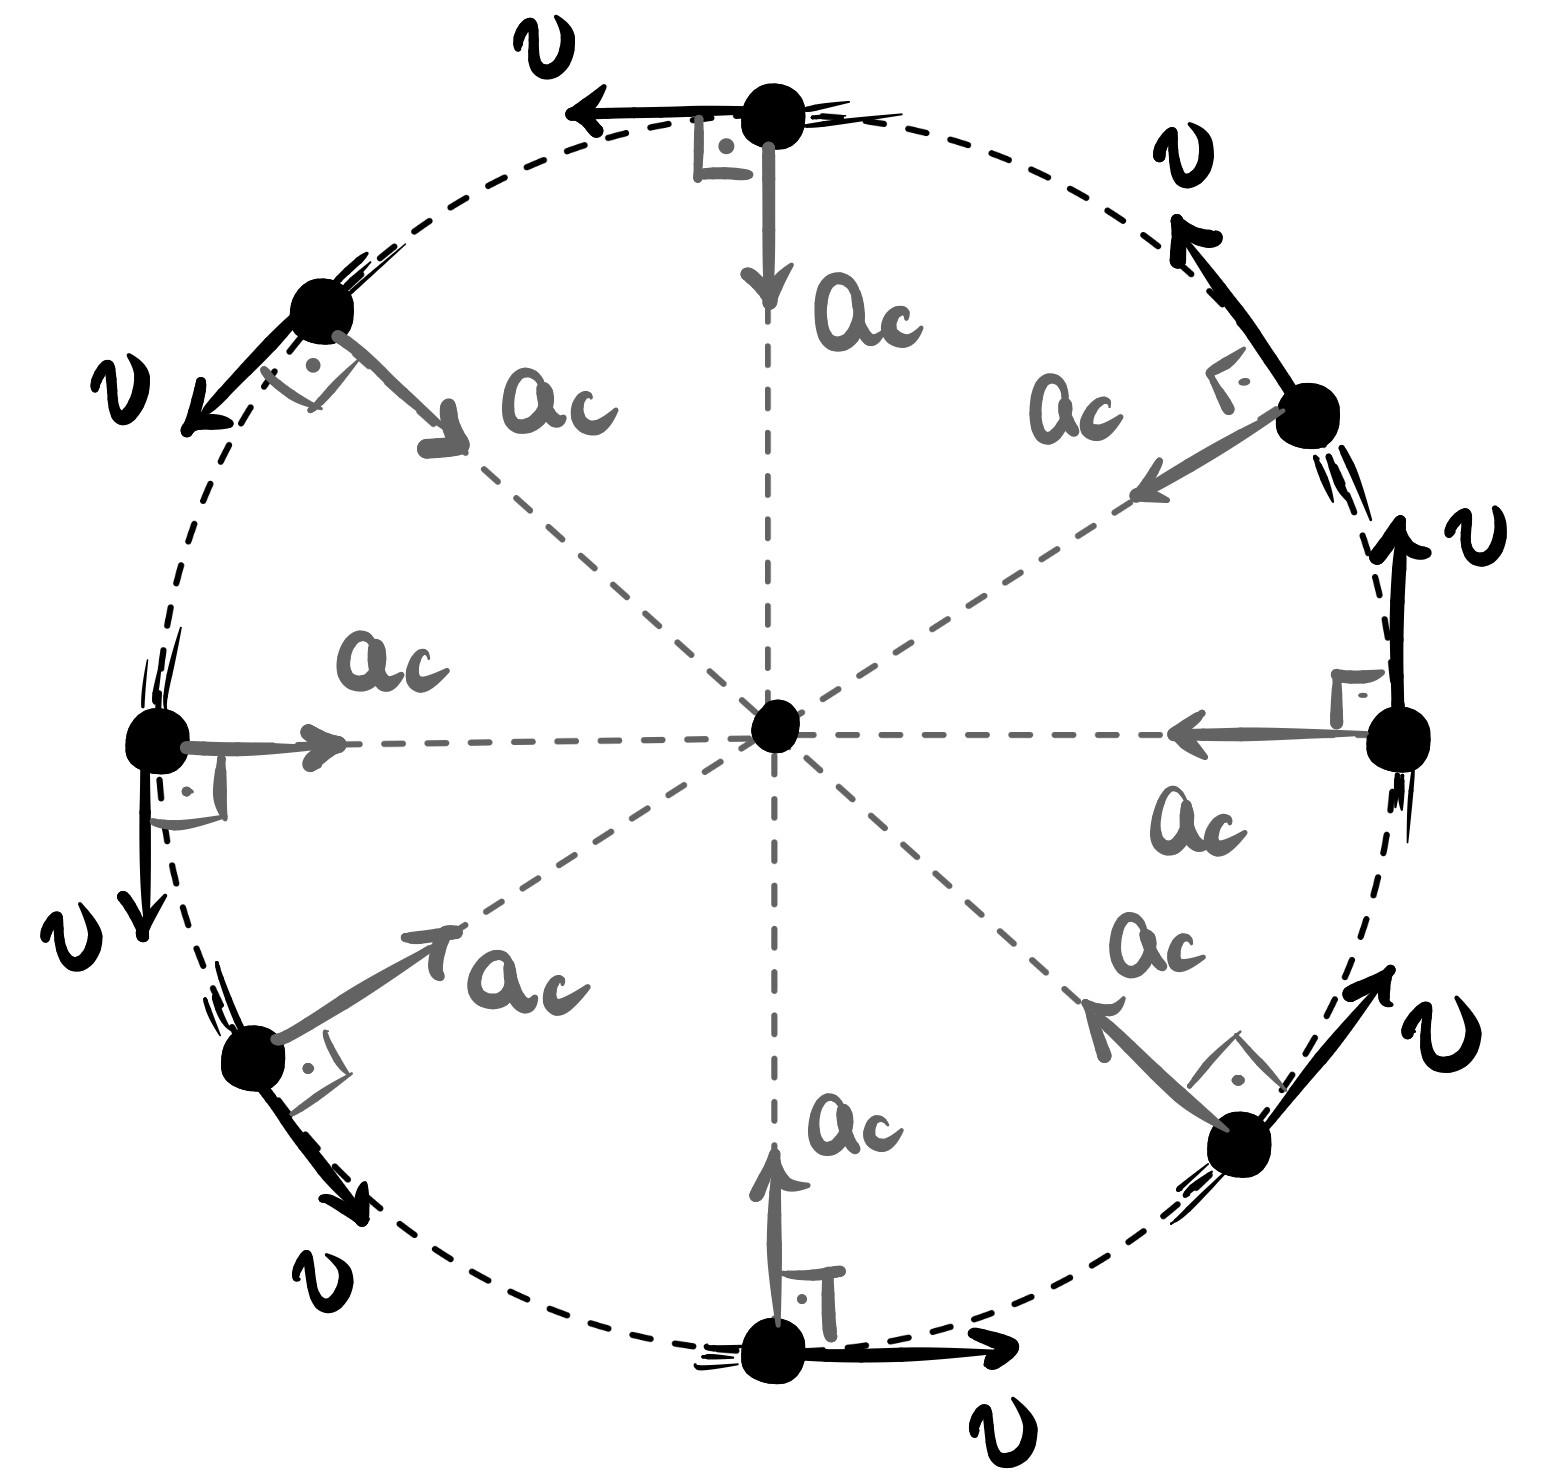
\includegraphics[width=0.4\linewidth]{imagenscinematicavetorial/acentripetaapontaparacentro2.jpeg}
\captionof{figure}{A aceleração centrípeta é sempre perpendicular à velocidade, apontando para o centro de curvatura em cada instante.}
\label{fig_cinvet_acentripetaapontaparacentro2}
} 

\end{enumerate}



\secgfe{Onde é usada}

Em praticamente qualquer contexto em que haja um movimento circular. Na verdade, o movimento sequer precisa ser circular: como a aceleração centrípeta é a responsável por alterar a direção do vetor velocidade, em absolutamente qualquer movimento que faça curva -- seja essa curva um arco de circunferência ou qualquer outra figura geométrica -- a aceleração centrípeta estará presente, garantindo que seja possível haver tal mudança de direção. Os movimentos circulares, por serem figuras geométricas mais simples, costumam ser os casos de aplicação mais comuns.

A Figura \ref{fig_cinvet_acentripetaexemplos} ilustra, para diferentes tipos de trajetórias curvilíneas, o vetor aceleração centrípeta -- sempre perpendicular à velocidade e apontando na direção radial, no sentido do centro de curvatura.

\vspace{0.3cm}
{
\centering
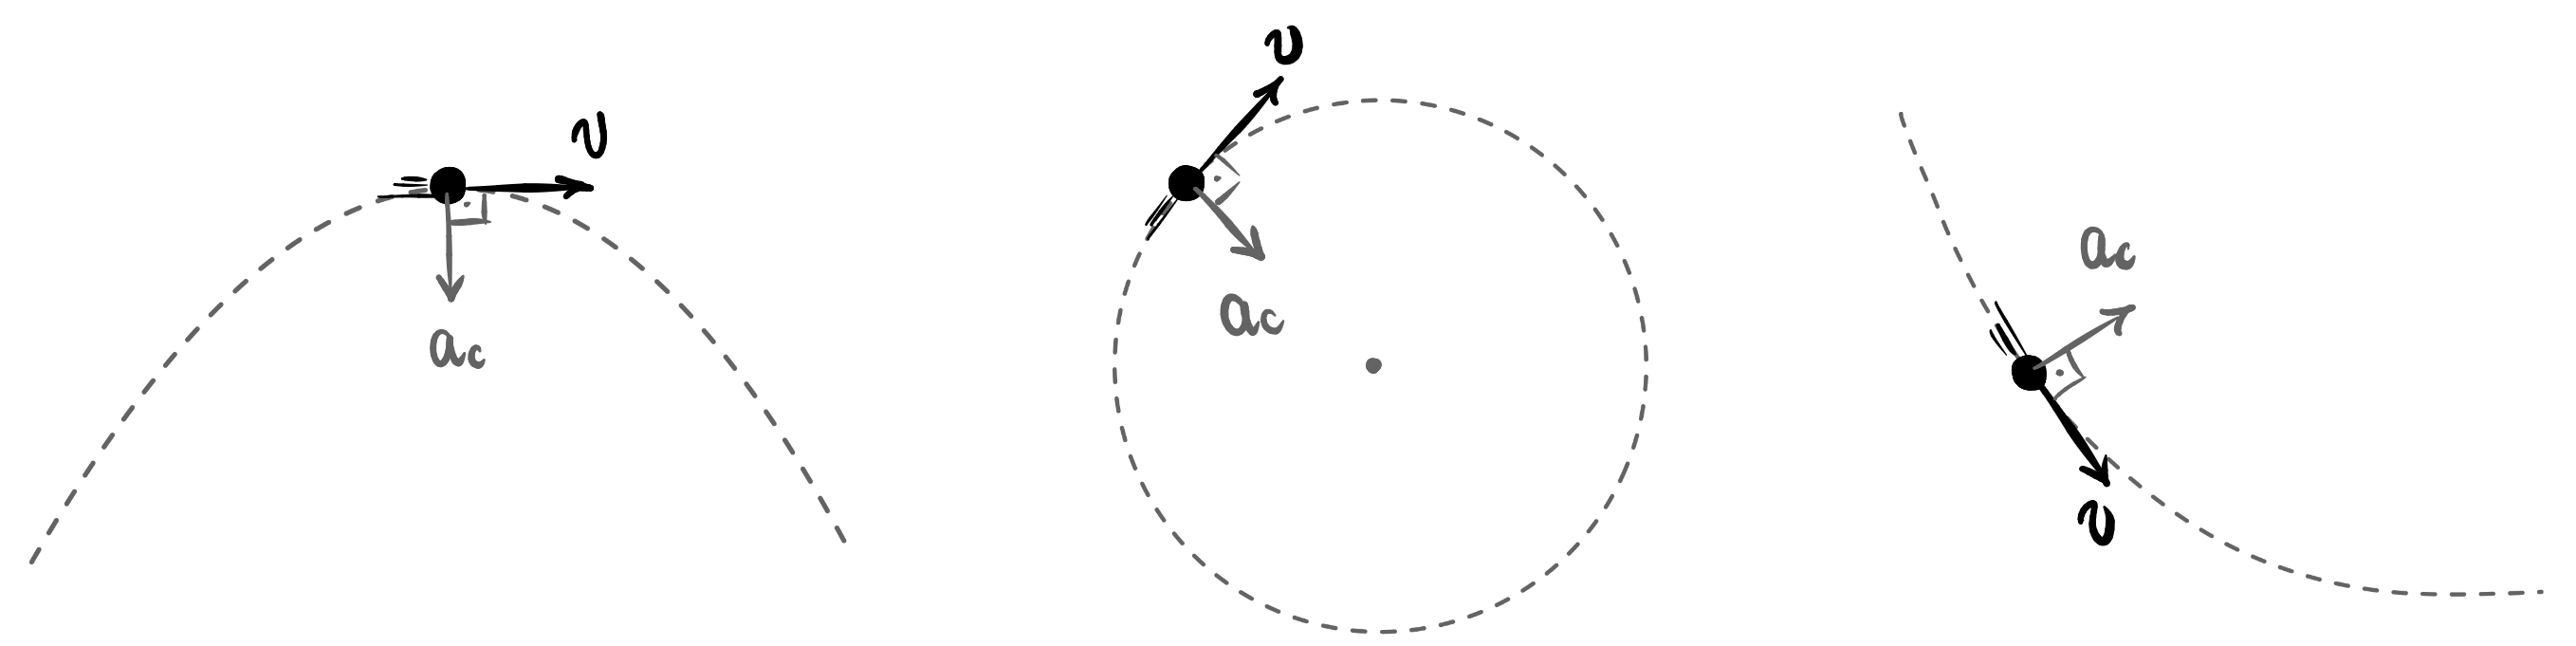
\includegraphics[width=0.8\linewidth]{imagenscinematicavetorial/acentripetaexemplos.jpeg}
\captionof{figure}{O vetor aceleração centrípeta em diferentes tipos de trajetória.}
\label{fig_cinvet_acentripetaexemplos}
} 


\secgfe{Erros comuns}

O erro mais comum aqui não costuma ser exatamente na aplicação e desenvolvimento de cálculos a partir da Equação \eqref{cinvet_eq_aceleracaocentripeta}, mas sim no entendimento claro do que ela calcula. Desse modo, correndo o risco de ser repetitivo, cabe destacar que tal equação \textbf{não calcula a aceleração de um corpo,} mas sim uma \textbf{componente específica de sua aceleração} -- aquela componente que é perpendicular à trajetória (e, portanto, perpendicular à velocidade) e aponta para o centro de curvatura. 

Tal componente, como já exposto, tem a função de alterar exclusivamente a direção do vetor velocidade, e não o seu módulo. Logo, em movimentos:




\begin{enumerate}
    \item [(i)] \textbf{retilíneos}, com certeza não haverá aceleração centrípeta, isto é

   $$ \boxed{\text{ movimento retilíneo $\Leftrightarrow a_c = 0$.}}$$

 Ou seja, vale a ida e a volta: se o movimento é retilíneo isso implica, necessariamente, que a aceleração centrípeta é nula; e se em um movimento a aceleração centrípeta for nula, então necessariamente tal movimento deve ser retilíneo.

     \item [(ii)] \textbf{curvilíneos} -- qualquer que seja o formato geométrico da curva -- a aceleração centrípeta nunca será nula:
     
        $$ \boxed{\text{ movimento curvilíneo $\Leftrightarrow a_c \neq 0$ .}}$$

        Novamente,  vale a ida e a volta: se o movimento faz curva isso implica, necessariamente, que a aceleração centrípeta não é zero; e se em um movimento a aceleração centrípeta for não nula, então necessariamente tal movimento deve ser curvilíneo.
\end{enumerate}


\secgfe{Observações}

A unidade de medida no SI da aceleração centrípeta é a mesma da aceleração escalar, que é $\text{m}\cdot\text{s}^{-2}.$ Afinal de contas, a aceleração centrípeta é apenas uma componente da aceleração -- a componente responsável por alterar a direção do vetor velocidade --, sendo, portanto, mensurada exatamente na mesma unidade de medida que já conhecíamos.

\vspace{0.3cm}

\begin{exemplo}[Nível I (UFSM)]

A figura representa dois atletas numa corrida, percorrendo uma curva circular, cada um em uma raia. Eles desenvolvem velocidades lineares com módulos iguais e constantes, num referencial fixo no solo. Atendendo à informação dada, assinale a resposta correta.

\begin{center}
\begin{tikzpicture}[scale=0.75]

% centro dos semicírculos
\coordinate (O) at (4,0);

% semicírculos concêntricos em escala de cinza
\fill[gray!55] (O) ++(180:3.6) arc[start angle=180,end angle=90,radius=3.6] --
               ++(0,-0.6) arc[start angle=90,end angle=180,radius=3.0] -- cycle;

\fill[gray!20] (O) ++(180:3.0) arc[start angle=180,end angle=90,radius=3.0] --
               ++(0,-0.6) arc[start angle=90,end angle=180,radius=2.4] -- cycle;

\fill[gray!55] (O) ++(180:2.4) arc[start angle=180,end angle=90,radius=2.4] --
               ++(0,-0.6) arc[start angle=90,end angle=180,radius=1.8] -- cycle;

\fill[gray!20] (O) ++(180:1.8) arc[start angle=180,end angle=90,radius=1.8] --
               ++(0,-0.6) arc[start angle=90,end angle=180,radius=1.2] -- cycle;

\fill[gray!55] (O) ++(180:1.2) arc[start angle=180,end angle=90,radius=1.2] --
               ++(0,-0.6) arc[start angle=90,end angle=180,radius=0.6] -- cycle;

% disco central
\fill[gray!65] (O) circle (0.6);

% pontos A e B
\fill (2.65,0) circle (2pt);
\node[left] at (2.8,-0.35) {\small A};

\fill (2.25,0.35) circle (2pt);
\node[left] at (2.25,0.35) {\small B};

\end{tikzpicture}
\end{center}



% {
% \centering
% 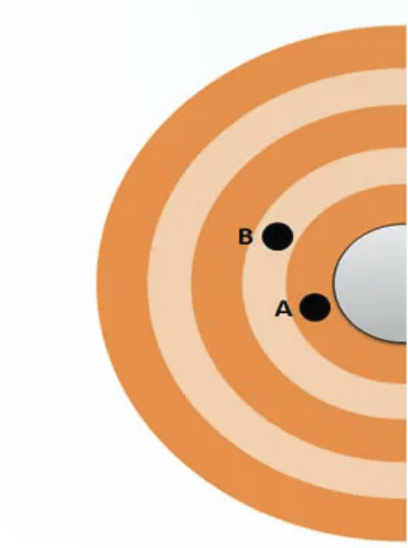
\includegraphics[width=0.15\linewidth]{imagenscinematicavetorial/ufsma_circular.png}
% \captionof{figure}{}
% \label{fig_cinvet_acentripetaufsm}
% } 

\begin{enumerate}
    \item [(a)] Em módulo, a aceleração centrípeta de A é maior do que a aceleração centrípeta de B.
    
    \item [(b)] Em módulo, as velocidades angulares de A e B são iguais.
    
    \item [(c)] A poderia acompanhar B se a velocidade angular de A fosse maior do que a de B, em módulo.
    
    \item [(d)] Se as massas dos corredores são iguais, a força centrípeta sobre B é maior do que a força centrípeta sobre A, em módulo.
    
    \item [(e)] Se A e B estivessem correndo na mesma raia, as forças centrípetas teriam módulos iguais, independentemente das massas.
\end{enumerate}


\resolucao

Avaliando o item $(a)$, sendo a aceleração centrípeta dada por $a_c = \sfrac{v^2}{R},$ e sendo as velocidades, em módulo, iguais, vemos que o indivíduo que percorrer a circunferência de menor raio -- indivíduo $A$, no caso -- terá maior aceleração centrípeta, haja vista que tais grandezas são inversamente proporcionais. \\

Logo, o item $(a)$ é o correto.

    
\end{exemplo}




\vspace{0.3cm}

\begin{exemplo}[Nível II]



Uma partícula descreve um movimento circular uniforme de raio $R$ e período $T$ em um plano horizontal. Em um certo instante, considera-se um sistema de eixos ortogonais fixos $x$ e $y$, tal que o vetor velocidade da partícula aponta exatamente na direção do eixo $y$.

Assinale a alternativa correta para as componentes da aceleração da partícula nesse instante.

\begin{enumerate}
\item [(a)] $a_x = 0$ e $a_y = \dfrac{4\pi^2 R}{T^2}$
\item [(b)] $a_x = -\dfrac{4\pi^2 R^2}{T^2}$ e $a_y = 0$
\item [(c)]$a_x = \dfrac{4\pi^2 R}{T^2}$ e $a_y = 0$
\item [(d)]$a_x = 0$ e $a_y = -\dfrac{4\pi^2 R}{T^2}$
\item [(e)]$a_x = -\dfrac{2\pi R}{T^2}$ e $a_y = \dfrac{2\pi R}{T^2}$
\end{enumerate}

\resolucao

A Figura \ref{fig_cinvet_aceleracaocentripetaexemplo02} ilustra a situação. Sendo o movimento uniforme, a aceleração será puramente centrípeta, apontando para o centro da circunferência, estando, portanto, alinhada com a direção $x.$ Logo, concluímos que $a_y=0$, de modo que descartamos as alternativas $(a)$, $(d)$ e $(e).$

{
\centering
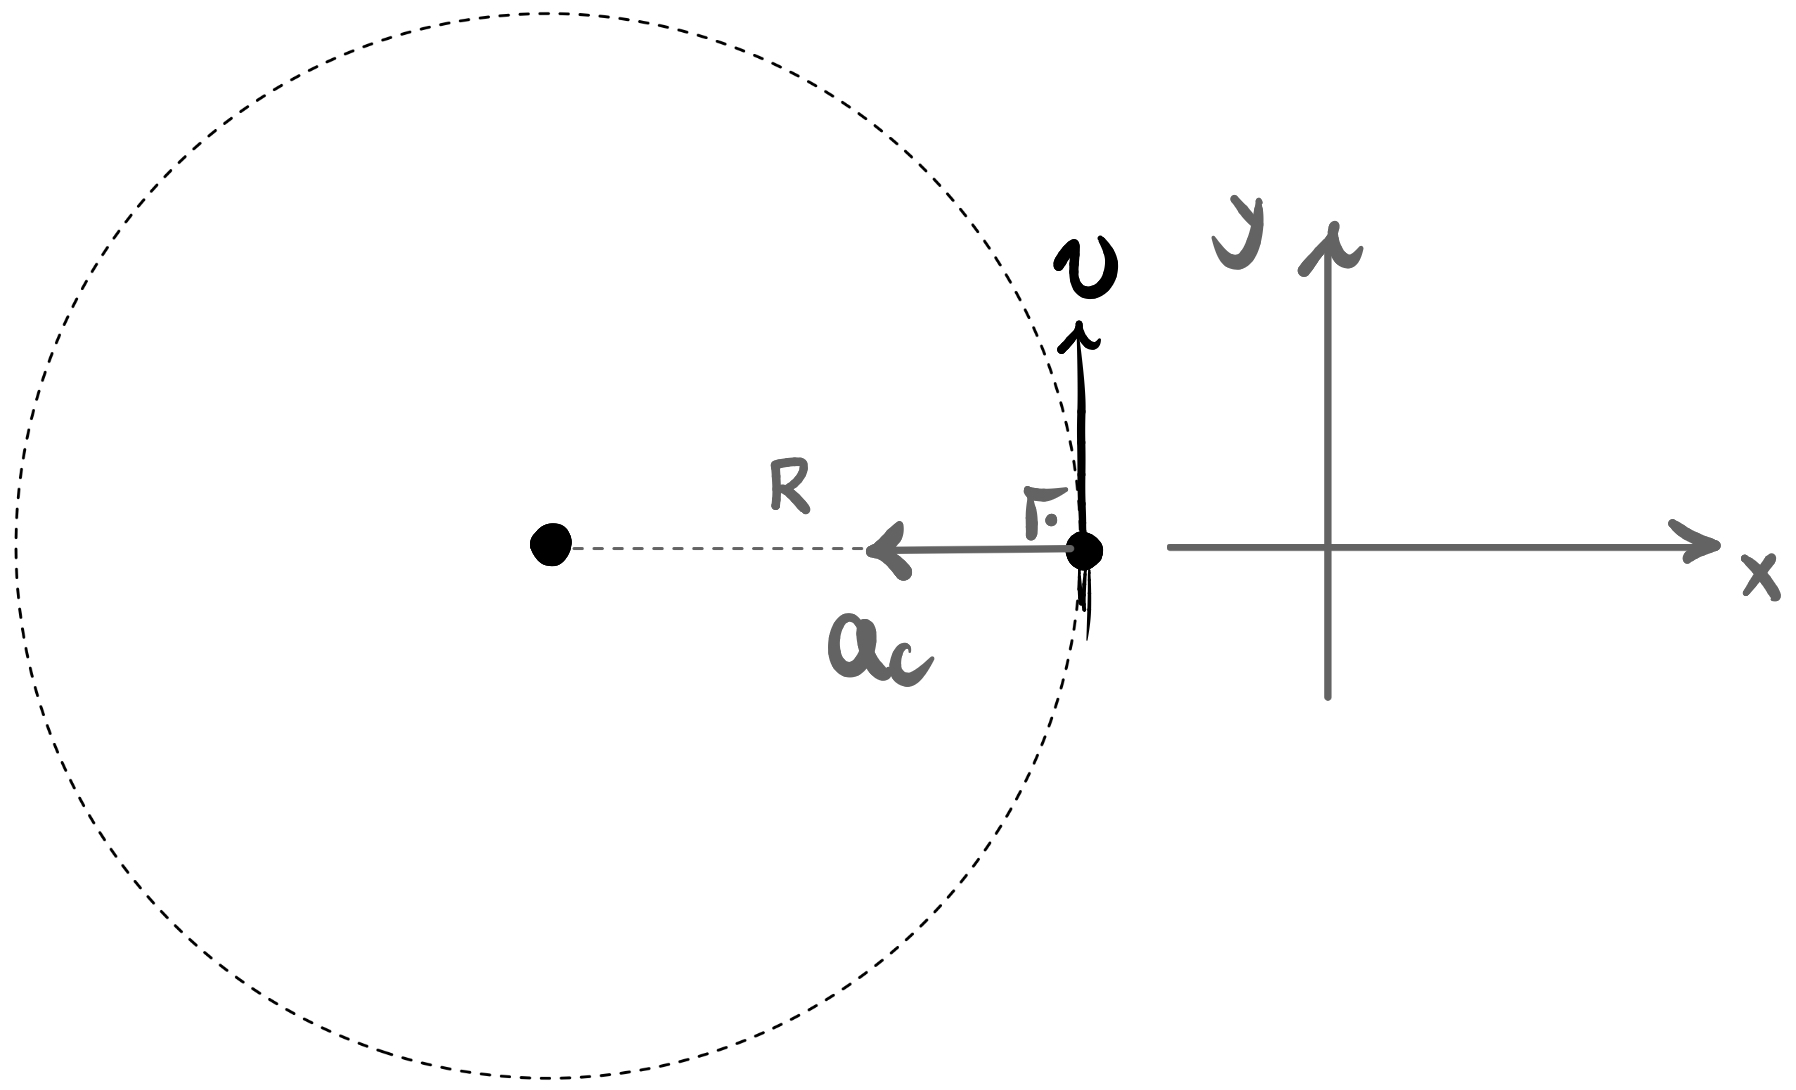
\includegraphics[width=0.4\linewidth]{imagenscinematicavetorial/aceleracaocentripetaexemplo02.jpeg}
\captionof{figure}{}
\label{fig_cinvet_aceleracaocentripetaexemplo02}
} 

A aceleração em $x$ será, portanto

$$ a_x =a_c = \dfrac{v^2}{R},$$

\noindent e, sendo o movimento uniforme, podemos usar que $v=\sfrac{d}{t}.$ Sendo $T$, o período, o tempo de uma volta, teremos que neste intervalo de tempo:

$$ v= \dfrac{d}{t} = \dfrac{2 \pi R}{T} \implies v^2 = \dfrac{4 \pi^2 R^2}{T^2},$$

\noindent e a aceleração em $x$ é, portanto,

$$ a_x = a_c = \dfrac{v^2}{R} = \dfrac{\dfrac{4 \pi^2 R^2}{T^2}}{R} \implies \boxed{a_x = \dfrac{4 \pi^2 R}{T^2},}$$

\noindent de modo que a resposta correta é a letra $(c).$
    
\end{exemplo}




\vspace{0.3cm}

\begin{exemplo}[Nível III]


Demonstre a Equação \eqref{cinvet_eq_aceleracaocentripeta} usando o conceito de aceleração escalar nas direções horizontal e vertical, computando a sobreposição desses efeitos para obter a aceleração que faz variar a direção do vetor velocidade.

\resolucao

A ideia aqui é fazer uma análise semelhante ao que fizemos no final da resolução do primeiro exemplo sobre e Equação \eqref{cinvet_eq_aceleracaovetorialmedia}, a qual convidamos que o leitor revisite para conectar melhor as ideias aqui desenvolvidas.

\vspace{0.3cm}
{
\centering
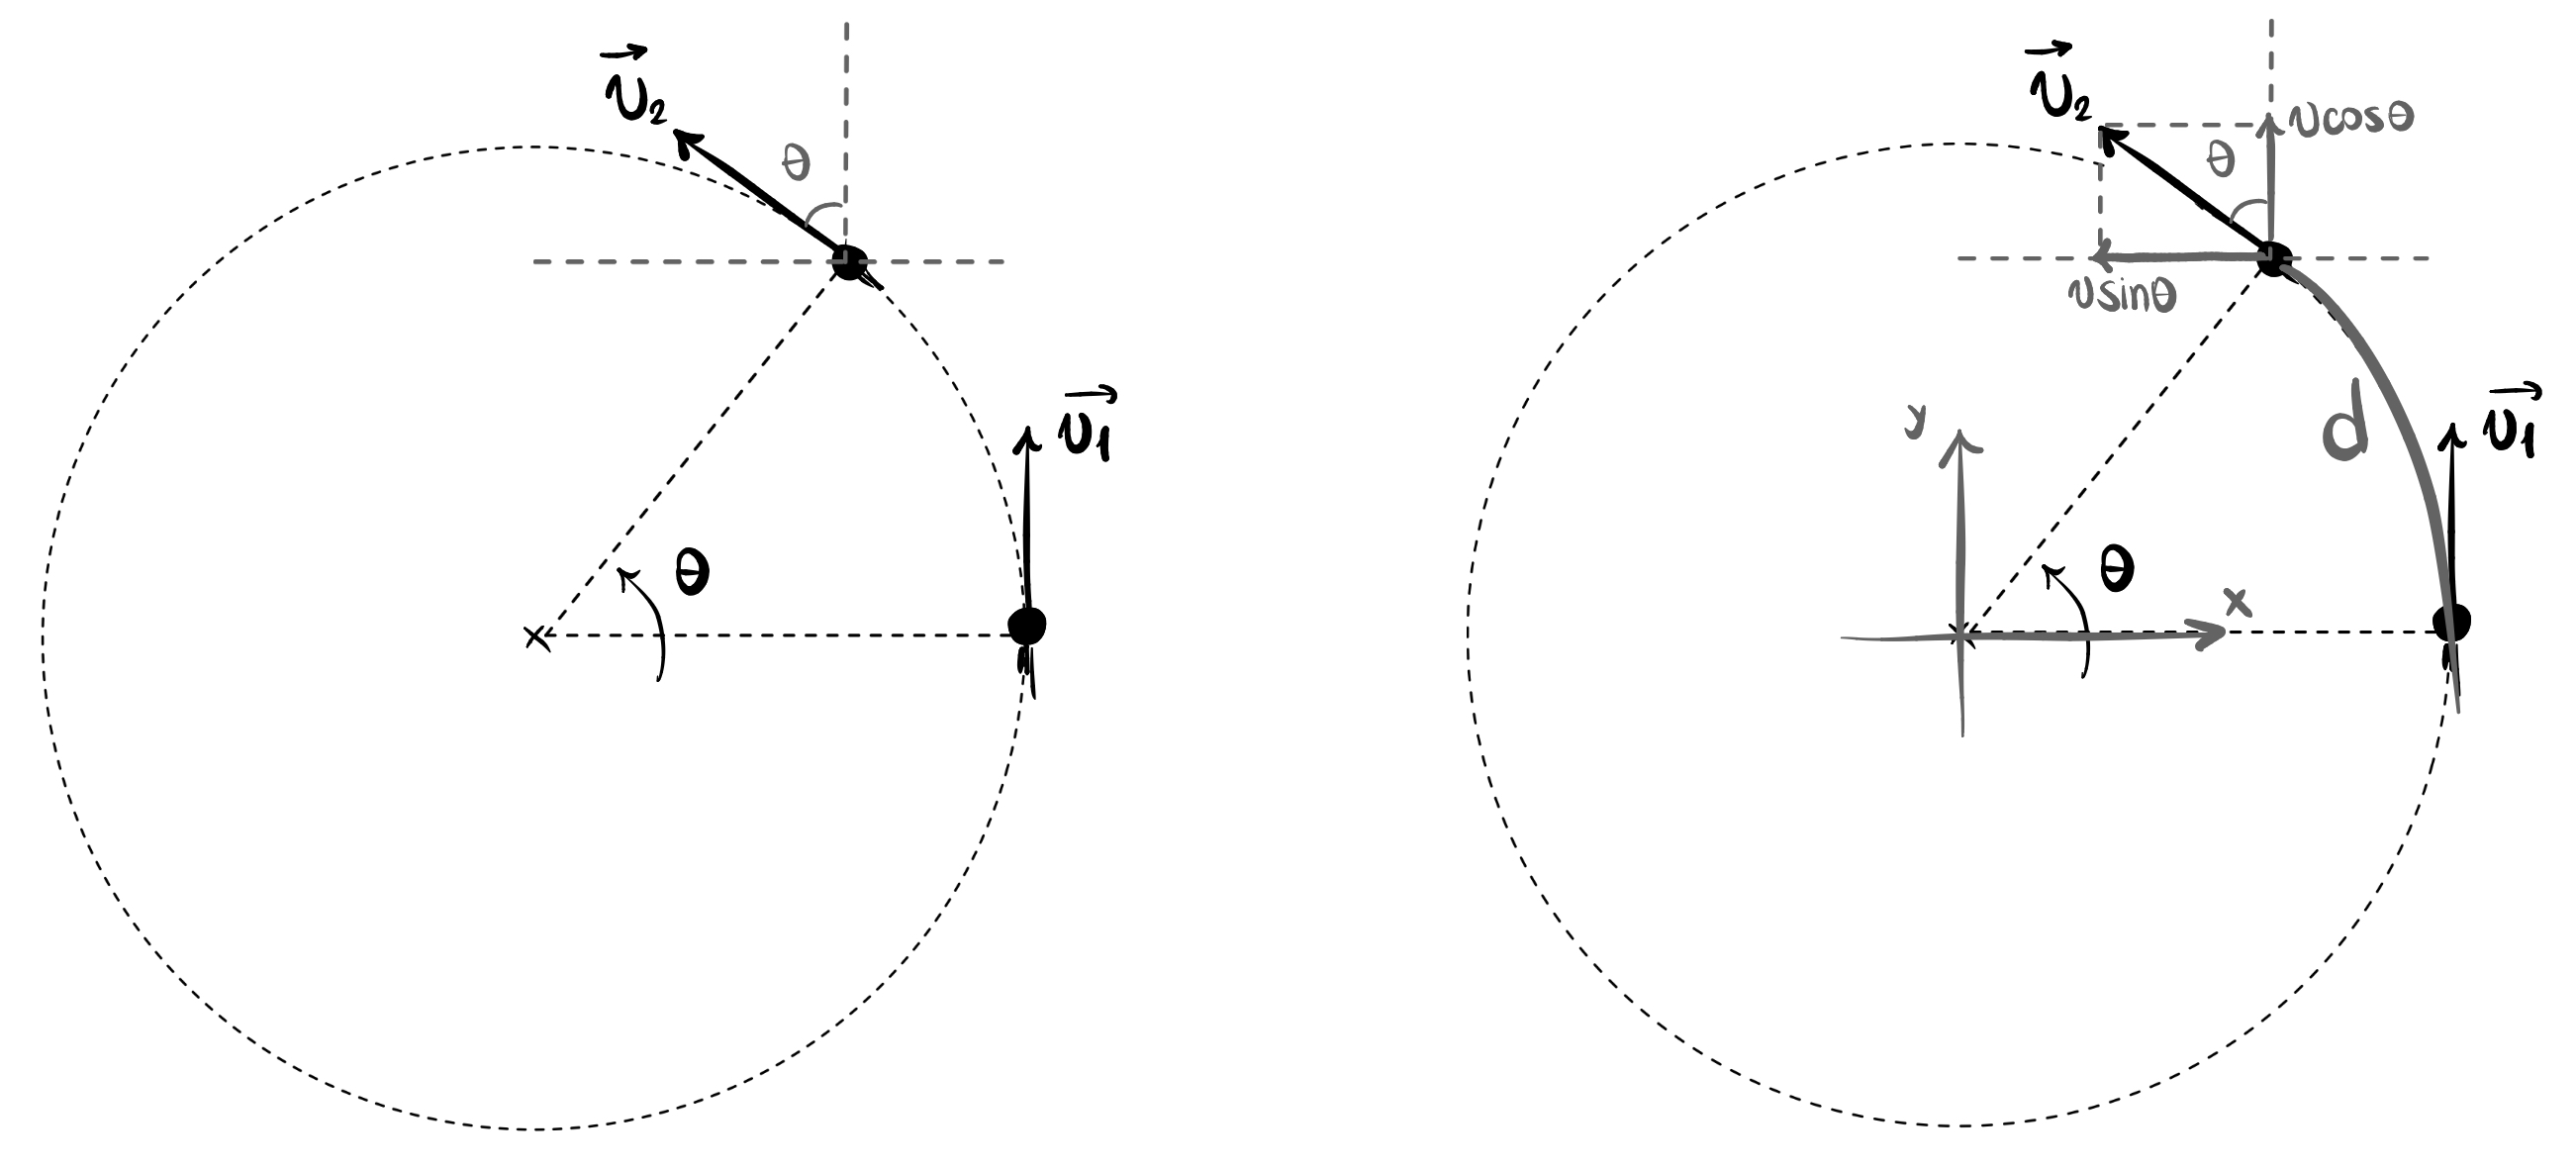
\includegraphics[width=0.8\linewidth]{imagenscinematicavetorial/aceleracaocentripetaexemplonivel3.jpeg}
\captionof{figure}{}
\label{fig_cinvet_aceleracaocentripetaexemplonivel3}
} 

Considere a primeira imagem da Figura \ref{fig_cinvet_aceleracaocentripetaexemplonivel3}, que mostra dois instantes de uma partícula que executa um MCU. Por ser um movimento uniforme, sabemos que 

$$ | \vec{v}_1| =  | \vec{v}_2| = v.$$

Entre os dois instantes $t_1$ e $t_2$, vamos considerar que atuam acelerações escalares nas duas direções $x$ e $y$, dadas por $a_x$ e $a_y,$ respectivamente. Com isso, calculamos a variação da velocidade em cada direção, o que aparece ilustrado na segunda imagem da Figura \ref{fig_cinvet_aceleracaocentripetaexemplonivel3}:

$$ \Delta v_x = -v \sin \theta - 0 \implies \boxed{ |\Delta v_x| = v \sin \theta}  \text{ e }  \Delta v_y = v \cos \theta - v \implies \boxed{ |\Delta v_y| = v  (1 - \cos \theta).} $$


Com isso, calculamos o módulo da aceleração escalar em cada direção, dado por

$$ |a_x| = \dfrac{|\Delta v_x|}{\Delta t} \implies \boxed{|a_x| = \dfrac{v \sin \theta}{\Delta t}} \quad \text{ e } \quad |a_y| = \dfrac{|\Delta v_y|}{\Delta t} \implies \boxed{|a_y| = \dfrac{v (1- \cos \theta)}{\Delta t}.}$$

Sendo as duas componentes perpendiculares, calculamos a aceleração resultante por meio do Teorema de Pitágoras:

$$ |\vec{a}|^2 = |a_x|^2 + |a_y|^2 \implies |\vec{a}|= \dfrac{v^2(\sin^2 \theta + 1 -2 \cos \theta + \cos^2 \theta)}{\Delta t},$$

\noindent que, usando a transformação do arco-metade $\sin^2 (\sfrac{\theta}{2}) = \sfrac{(1- \cos \theta)}{2},$ nos leva a

$$ |\vec{a}|= \dfrac{2v \sin (\sfrac{\theta}{2})}{\Delta t}. $$

Sendo o movimento uniforme, podemos escrever que $d=v \Delta t.$ Contudo, pela definição de radiano, temos que $\theta = \sfrac{d}{R},$ de modo que chegamos que

$$ \theta = \dfrac{v \Delta t}{R},$$

  \noindent assim, temos

  $$ |\vec{a}|= \dfrac{2v \sin (\sfrac{v \Delta t}{2R})}{\Delta t}.$$

  Por fim, como faremos a análise para um intervalo de tempo muito pequeno de modo a obter a aceleração vetorial em um instante, e não uma aceleração média entre intervalos de tempos distantes, o ângulo $\theta,$ como discutido anteriormente, será muito, muito pequeno. Usando a aproximação para ângulo pequenos $\sin \theta \approx \theta,$ que vale para $\theta$ em radianos, teremos

   $$\sin \left( \dfrac{v \Delta t}{2R} \right) \approx \dfrac{v \Delta t}{2R}, $$

   \noindent o que nos leva finalmente a

    $$ |\vec{a}|= \dfrac{2v \sin (\sfrac{v \Delta t}{2R})}{\Delta t} = \dfrac{2v}{\Delta t} \cdot \dfrac{v \Delta t}{2R} \implies \boxed{|\vec{a}|=\dfrac{v^2}{R},} $$

    \noindent como queríamos demonstrar.
  

    
\end{exemplo}




%Exemplo resolvido











\begin{secnivel}[Aceleração Tangencial]{I}{Aceleração Tangencial}
  
  \eqLdois{def}{cinvet_eq_aceleracaotangencialmedia}{a_t= a_m}

\end{secnivel}







\secgfe{De onde vem}

A bem da verdade, a Equação \eqref{cinvet_eq_aceleracaotangencialmedia} não é uma equação nova, mas sim uma reestruturação de um conceito que já conhecíamos -- o de aceleração escalar, aquela que faz variar o módulo do vetor velocidade. Tal equação está dizendo que este novo conceito que construiremos aqui -- o de aceleração tangencial, representada por $a_t$ -- coincide com o conceito de aceleração escalar que havíamos definido na Equação \eqref{mecanica_eq_aceleracaomedia}.

\vspace{0.3cm}
{
\centering
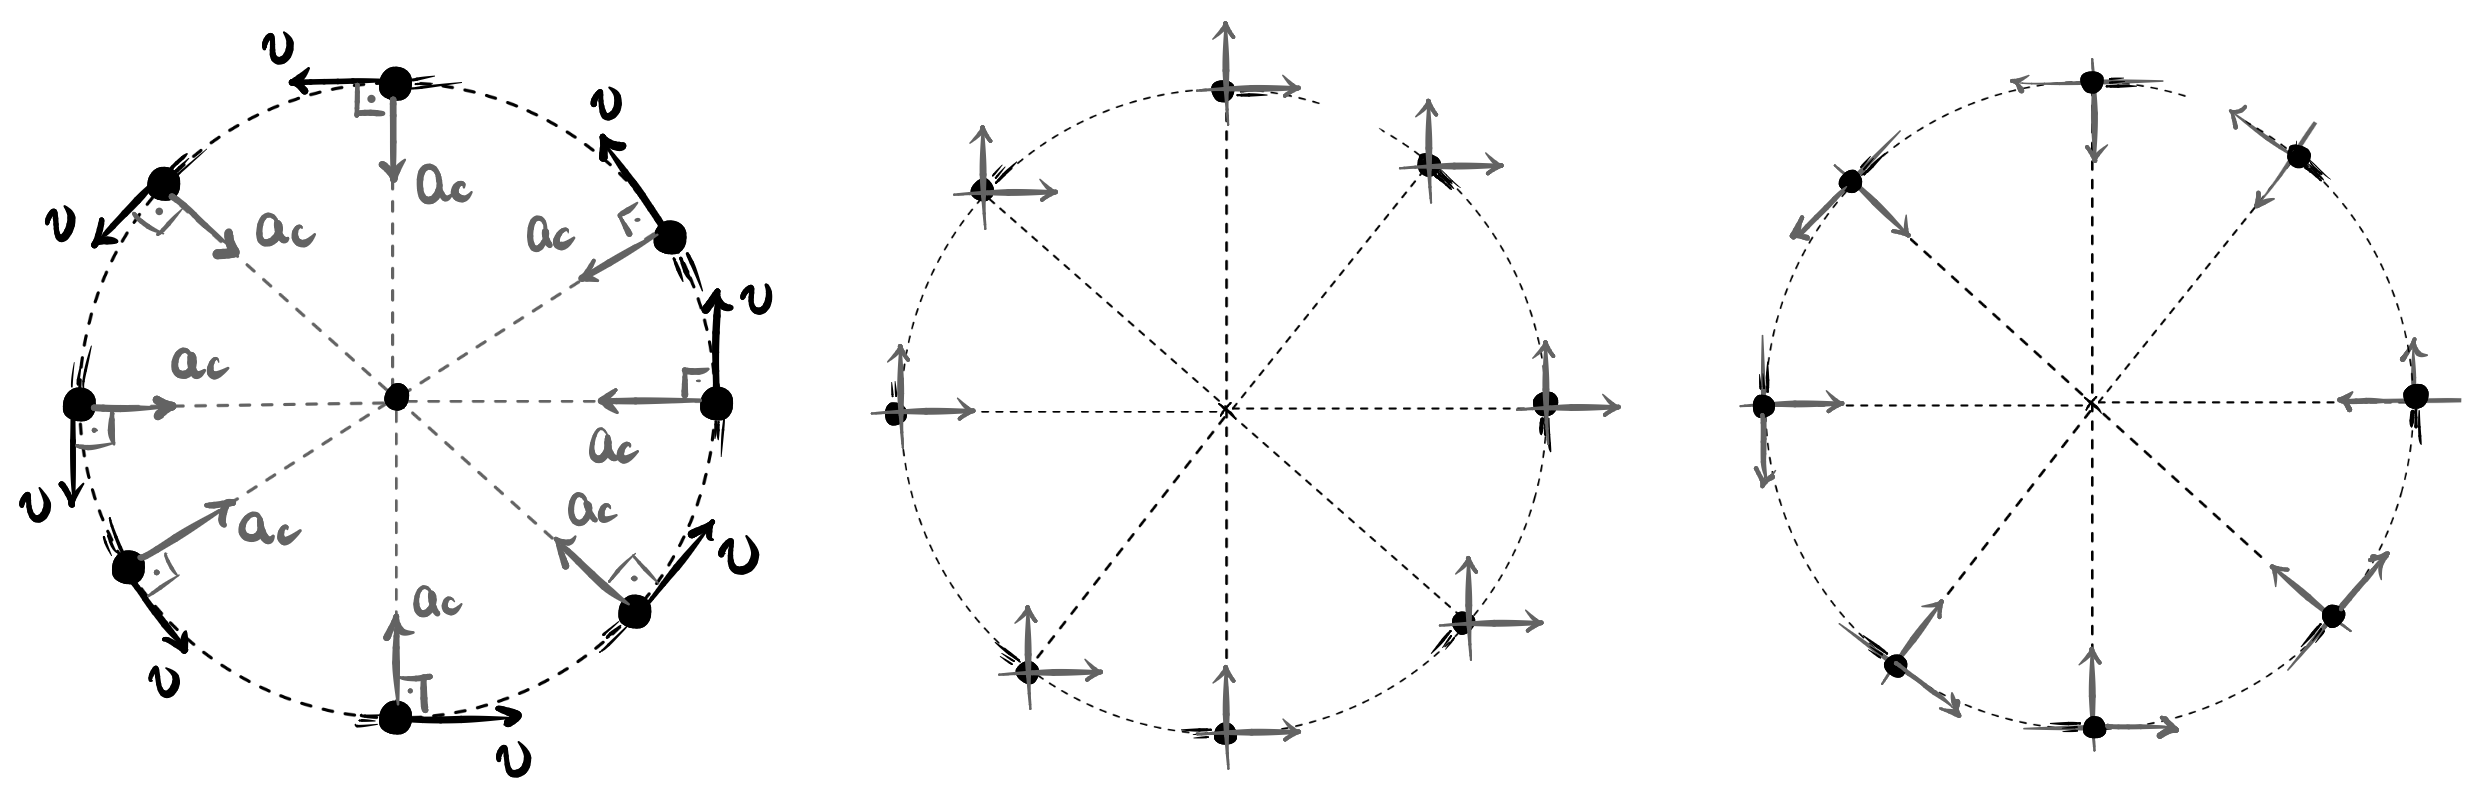
\includegraphics[width=0.9\linewidth]{imagenscinematicavetorial/aceleracaotangencial1.png}
\captionof{figure}{Os eixos mais adequados para fazer a análise das grandezas vetoriais em um movimento curvilíneo são os eixos centrípeto e tangencial.}
\label{fig_cinvet_aceleracaotangencial1}
} 
\vspace{0.3cm}

Relembre, pela Figura \ref{fig_cinvet_aceleracaotangencial1}, o que construímos até aqui: em um movimento curvilíneo a velocidade é sempre tangente à trajetória, e em tal movimento sempre há, pelo menos, um tipo de aceleração -- a aceleração responsável por variar a direção do vetor velocidade e possibilitar, portanto, que o corpo em movimento faça curva. Tal aceleração aponta sempre para o centro de curvatura, como vimos.




Note que a imagem do meio mostra uma escolha ruim de eixos ortogonais para se decompor e fazer a análise das grandezas vetoriais do problema -- um sistema de eixos fixo, vertical e horizontal. Tal sistema é ruim porque, como já vimos, todas as grandezas vetoriais estudadas até aqui em tal movimento se dão ao longo da direção tangencial e direção radial (centrípeta). Sendo assim, é muito mais conveniente adotar um sistema de eixos perpendiculares em que um deles está alinhado com a direção centrípeta e o outro com a direção tangencial.

É claro que, enquanto as direções vertical e horizontal são fixas, as direções tangencial e radial são variáveis, como mostra a terceira imagem da \ref{fig_cinvet_aceleracaotangencial1}. Desse modo, é como se nosso par de eixos ortogonais, ao invés de ser fixo, girasse junto com a partícula em movimento. Ou, caso o leitor prefira, é como se tivéssemos vários sistemas de coordenadas diferentes, um para cada ponto do movimento da partícula, sendo seus eixos sempre perpendiculares e alinhados com as direções tangente e radial à circunferência naquele ponto.

Dito isso, o que aconteceria se tivéssemos um movimento curvilíneo, em que a velocidade muda não apenas de direção, mas também tem o seu módulo alterado? Ora, se concluímos que existe um tipo de aceleração $a_c$ -- que aponta para o centro -- cujo único efeito é alterar a direção da velocidade, então é natural esperar que a aceleração $a_t$, cujo efeito será alterar o valor de tal velocidade, esteja em uma direção complementar àquela, no caso, na direção tangente à trajetória.

\vspace{0.3cm}
{
\centering
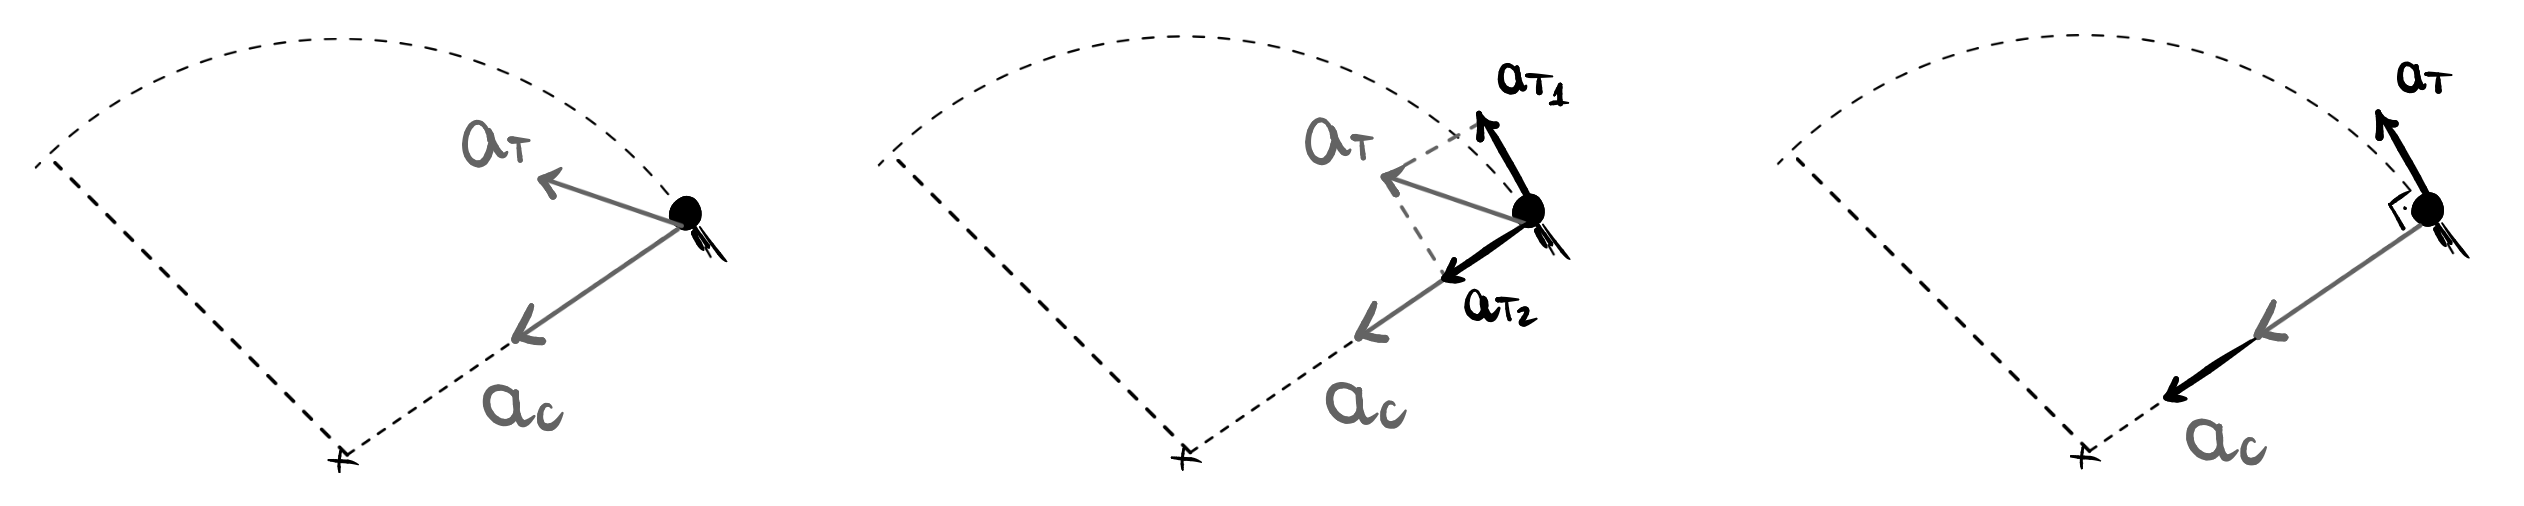
\includegraphics[width=0.9\linewidth]{imagenscinematicavetorial/aceleracaotangencial15.png}
\captionof{figure}{A aceleração responsável por alterar o módulo do vetor velocidade é paralela a tal vetor, sendo, portanto, tangente à trajetória.}
\label{fig_cinvet_aceleracaotangencial15}
} 
\vspace{0.3cm}

Para capturar bem este conceito, observe a Figura \ref{fig_cinvet_aceleracaotangencial15}. Nela, estamos assumindo que temos um movimento em que o vetor velocidade varia não apenas em direção, mas também em módulo. Já conhecemos a componente de aceleração responsável por variar a direção, é a componente $a_c,$ que aponta para o centro. Digamos que agora estamos querendo compreender como funciona a componente de aceleração $a_t$ responsável por alterar o módulo do vetor velocidade. Assim, suponha que tal componente atue sempre em uma direção oblíqua, fazendo um certo ângulo com o vetor $\vec{a}_c.$ Ora, neste caso, seria possível decompor tal vetor nas direções radial e tangencial, como mostra a segunda imagem da figura. Com isso, notaríamos que a componente de tal vetor na direção centrípeta na verdade trata-se de uma contribuição para a aceleração centrípeta, ou seja, é um tipo de aceleração que não altera o módulo do vetor velocidade. Assim sendo, a aceleração que nos restaria -- aquela que deve ser a responsável por alterar apenas o módulo do vetor velocidade -- é justamente aquela componente que se encontra integralmente na direção tangencial.




Sendo assim, concluímos aqui a essência do que diz a Equação \eqref{cinvet_eq_aceleracaotangencialmedia}: em movimentos bidimensionais que façam curvas, caso o módulo da velocidade mude, tal fato se dá devido à ação de uma componente de aceleração, chamada aceleração tangencial, que é tangente à trajetória -- e, portanto, paralela ao vetor velocidade -- e cuja ação está integralmente ligada à variação do valor da velocidade, de modo que o módulo de tal vetor pode ser computado por 

 $$ |\vec{a}_t| = \dfrac{\Delta v}{\Delta t},$$

\noindent que coincide justamente com o conceito de aceleração escalar que já conhecíamos, porém agora passando a incorporar o caráter vetorial -- a aceleração que muda o valor da velocidade deve ser sempre paralela à velocidade e, portanto, tangente à trajetória.

Observe que isso já ocorria nos casos unidimensionais antes estudados, no MUV: a nossa aceleração era sempre paralela à velocidade, podendo apontar no mesmo sentido -- casos em que o movimento seria acelerado e o valor da velocidade, portanto, aumentaria -- ou no sentido contrário -- casos em que o movimento era chamado de retardado e o valor da velocidade, portanto, diminuiria ao longo do tempo. De todo modo, a aceleração ali já respeitava essa condição de ser tangente à trajetória. Ocorre que, sendo a trajetória retilínea (movimento em uma dimensão) ser tangente a uma reta significa simplesmente que todos os vetores estão alinhados naquela mesma direção. Quando expandimos o estudo para movimentos bidimensionais é preciso estender este conceito, e é isso que o conceito de aceleração tangencial faz.


\vspace{0.3cm}
{
\centering
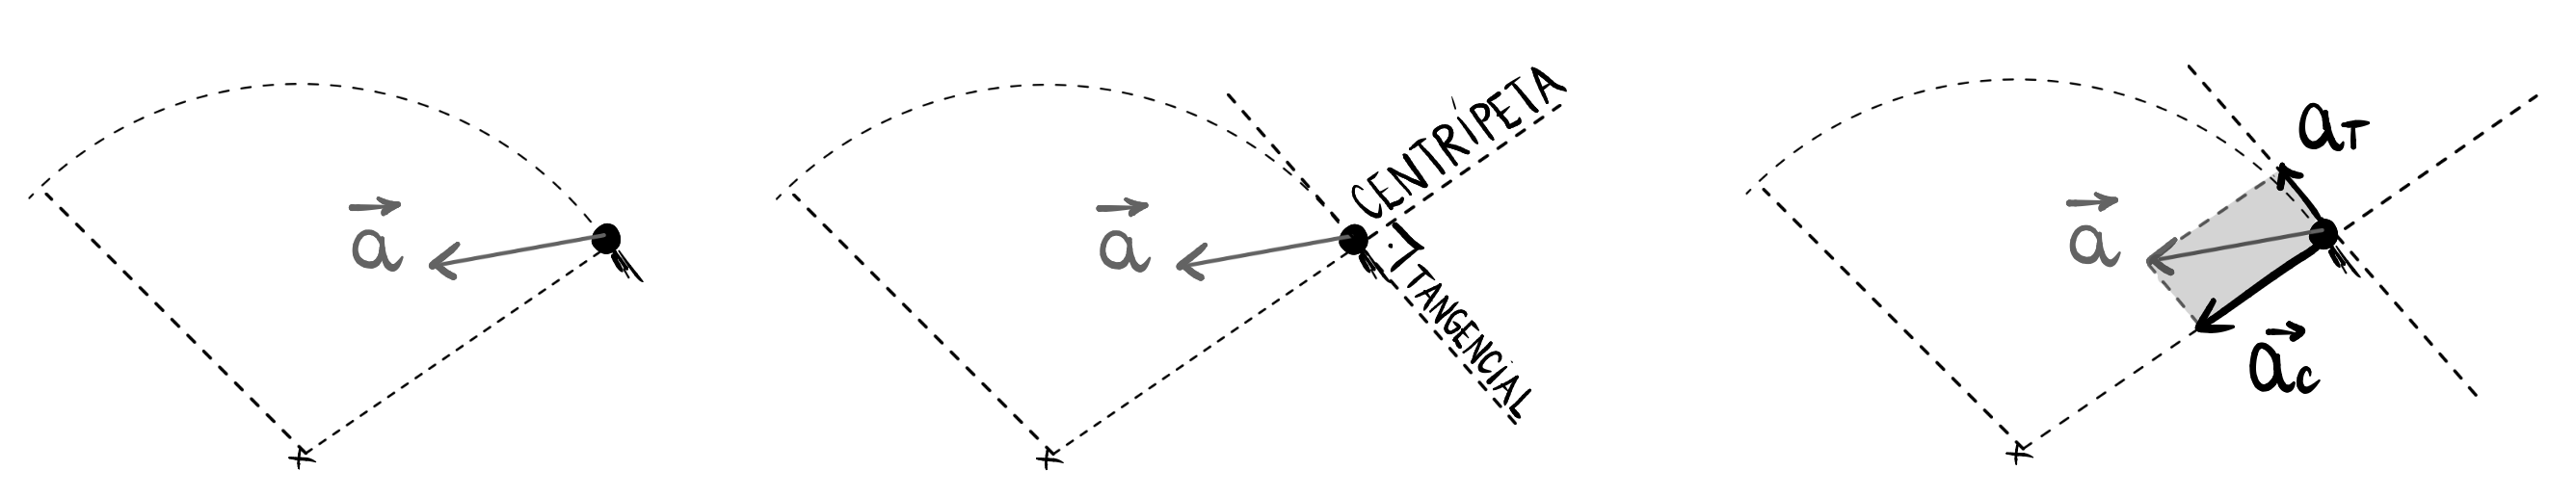
\includegraphics[width=0.9\linewidth]{imagenscinematicavetorial/aceleracaotangencial2.png}
\captionof{figure}{As componentes tangencial e centrípeta da aceleração.}
\label{fig_cinvet_aceleracaotangencial2}
} 
\vspace{0.3cm}

Por fim, observe que, de modo geral, o vetor aceleração $\vec{a}$ de uma partícula em um movimento qualquer pode apontar em uma direção qualquer, como mostra a primeira imagem da Figura \ref{fig_cinvet_aceleracaotangencial2}. Contudo, tal vetor sempre pode ser decomposto nas direções centrípeta e tangencial, resultando nas componentes $a_c$ e $a_t$ respectivamente. Cada uma dessas componentes pode ser computada e interpretada de forma separada, e o significado de cada uma delas já foi amplamente discutido e deve soar bem familiar leitor a essa altura.




Vale pontuar que, como os eixos centrípeto e radial são perpendiculares, os módulos das componentes $a_t$ e $a_c$ da aceleração $a$ podem ser relacionados pelo Teorema de Pitágoras:

$$ \boxed{a^2=a_t^2+a_c^2.}$$



\secgfe{Onde é usada}

Em problemas nos quais o \textbf{módulo da velocidade do corpo varia.} Perceba que, quando estudamos o MU e o MUV, sempre em linha reta, a aceleração que lá tratamos -- aceleração escalar -- é justamente o que, aqui, estamos chamando de aceleração tangencial: uma aceleração que atua na mesma direção do vetor velocidade e, portanto, faz variar o seu módulo, aumentando-o ou diminuindo-o.


\secgfe{Erros comuns}

O erro mais comum -- em se tratando de movimentos curvilíneos -- é quando o estudante insiste em fazer a análise das grandezas vetoriais nas direções horizontal e vertical. Como vimos na Figura \ref{fig_cinvet_aceleracaotangencial1}, as direções ideais que simplificam a análise são as direções centrípeta e radial, em cada ponto. A componente de aceleração na direção centrípeta será aquela responsável por variar a direção do vetor velocidade, e será computada pela Equação \eqref{cinvet_eq_aceleracaocentripeta}; enquanto a componente de aceleração na direção tangencial será responsável por variar o módulo do vetor velocidade, e será computada por meio da Equação \eqref{mecanica_eq_aceleracaomedia}.


\secgfe{Observações}

Vale pontuar que qualquer movimento que faça alguma curva será, certamente, um movimento acelerado: atua ali, pelo menos, a componente centrípeta da aceleração. Perceba, portanto que o movimento da primeira imagem da Figura \ref{fig_cinvet_aceleracaotangencialfinal} é acelerado, ainda que o valor da velocidade não mude.

\vspace{0.3cm}
{
\centering
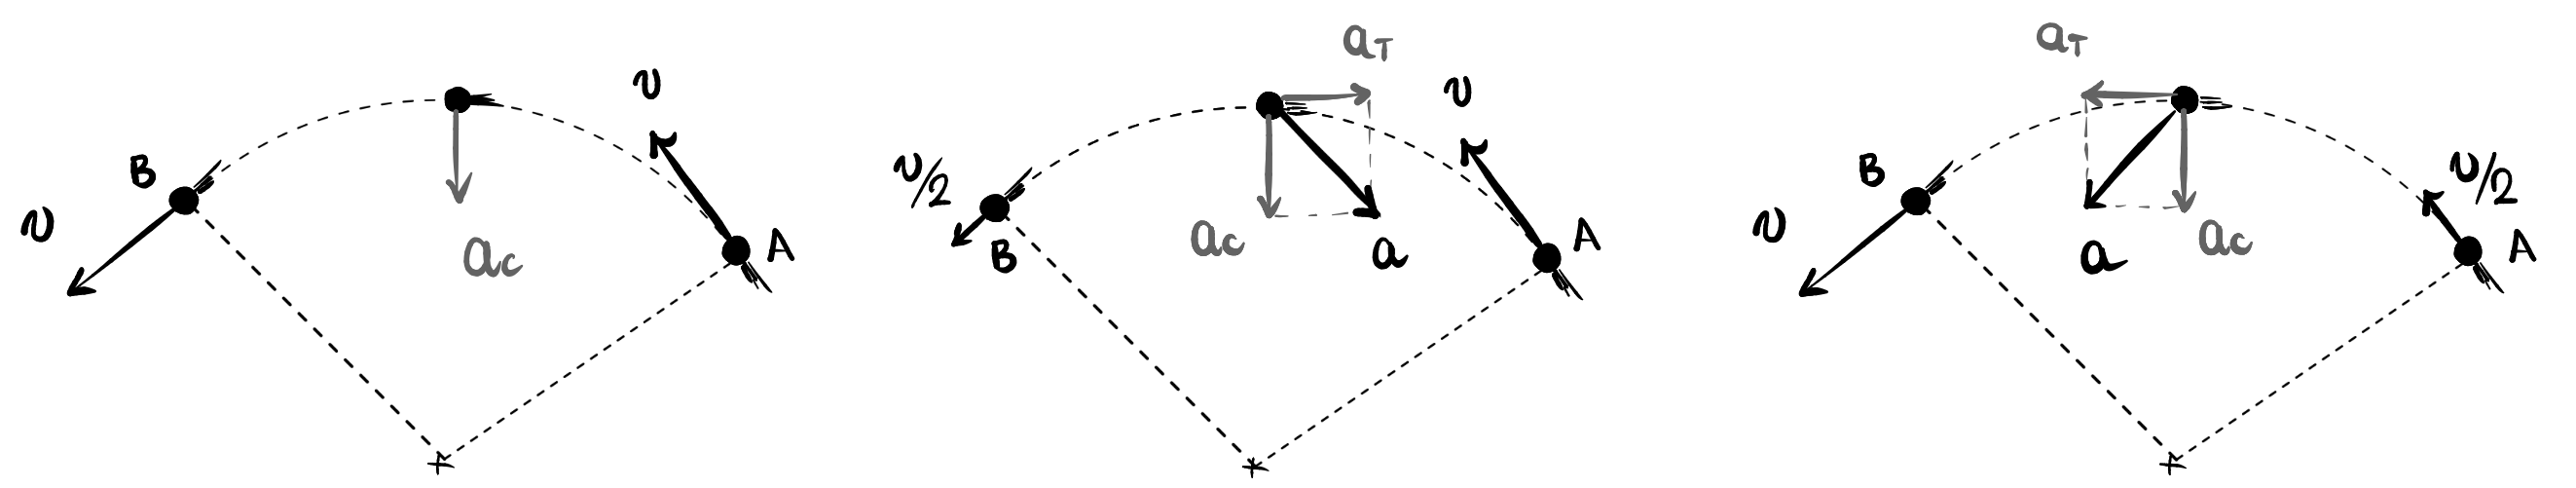
\includegraphics[width=0.9\linewidth]{imagenscinematicavetorial/aceleracaotangencialfinal.png}
\captionof{figure}{Os diferentes tipos de movimento acelerado.}
\label{fig_cinvet_aceleracaotangencialfinal}
} 
\vspace{0.3cm}

Já no movimento da imagem do meio, observamos que entre os pontos $A$ e $B$ a velocidade diminuiu. Logo, além da aceleração centrípeta, há também atuando ali a aceleração tangencial, retardando o movimento. Assim, a aceleração tangencial atua no sentido contrário ao da velocidade, contribuindo para que a aceleração resultante aponte para a direção oblíqua destacada naquele ponto intermediário do movimento.


No movimento da última imagem observamos que entre os pontos $A$ e $B$ a velocidade aumentou. Logo, além da aceleração centrípeta, há também atuando ali a aceleração tangencial, aumentando o valor da velocidade. Assim, a aceleração tangencial atua no mesmo sentido da velocidade, contribuindo para que a aceleração resultante aponte para a direção oblíqua destacada naquele ponto intermediário do movimento.




Os três movimentos da Figura \ref{fig_cinvet_aceleracaotangencialfinal} são, portanto, movimentos acelerados, uma vez que possuem algum tipo de aceleração. No primeiro o valor da velocidade é constante, então ele também pode ser chamado de movimento uniforme. No segundo o movimento seria retardado e no terceiro acelerado -- sendo essas classificações oriundas da componente tangencial da aceleração.

\vspace{0.3cm}

\begin{exemplo}[Nível I]\label{exemplo_cinematicavetorial_aceleracaotangencialex01}


Uma partícula se move em uma trajetória circular de raio $R=20.25$m. No instante $t=0$s sua velocidade é $v_0=3$ m/s, já no instante $t=2$s sua velocidade é $v=9$ m/s.

Se a taxa com que o valor da sua velocidade muda é constante, encontre, em $t=2$s

\begin{enumerate}
    \item [(a)] O módulo da aceleração tangencial da partícula.
    \item [(b)] O módulo da aceleração centrípeta da partícula.
    \item [(c)] O módulo da aceleração vetorial da partícula.
    
\end{enumerate}

\resolucao

\begin{enumerate}
   

 \item [(a)] A aceleração tangencial captura a informação de quanto varia o valor da velocidade da partícula, logo, tem-se

 $$ a_t = \dfrac{\Delta v}{\Delta t}=\dfrac{9-3}{2-0} \implies \boxed{a_t=3 \text{ m/s}^2.}$$

 \item [(b)] A aceleração centrípeta $a_c$ dependerá do valor exato da velocidade e, como este aumenta, o valor de $a_c$ será diferente em cada ponto. Em particular, para $t=2$s, teremos

  $$ a_c = \dfrac{v^2}{R} = \dfrac{9^2}{20.25} \implies \boxed{a_c= 4 \text{ m/s}^2.}$$

\item [(c)] A aceleração vetorial é o efeito resultante das acelerações calculadas anteriormente. Sendo as direções tangencial e centrípeta perpendiculares, o módulo $a$ do vetor aceleração média é obtido pela relação pitagórica

$$ a^2 = a_t^2+a_c^2 = 3^2+4^2 \implies \boxed{a= 5 \text{ m/s}^2.}$$
  \end{enumerate}
    
\end{exemplo}







\vspace{0.3cm}

\begin{exemplo}[Nível II]\label{exemplo_cinematicavetorial_aceleracaotangencialex02}

Uma partícula descreve uma trajetória circular de raio $R$. Seu movimento é tal que o módulo da aceleração total permanece constante, enquanto a velocidade escalar aumenta com o tempo. Sabendo que, em um certo instante, a velocidade da partícula é $v$, determine a aceleração tangencial $a_t$ nesse instante, em função de $v$, $R$ e do módulo constante $a$ da aceleração total.

\resolucao

Vamos primeiro tentar intuir o que deve acontecer: o valor da velocidade aumenta, logo, temos uma aceleração tangencial. Ora, mas se o valor de $v$ aumenta, então o valor $a_c$ da aceleração centrípeta também deve aumentar, uma vez que $a_c = \sfrac{v^2}{R},$ e o raio é mantido fixo.

Porém se o valor de $a_c$ aumenta, mas se o valor absoluto da aceleração vetorial é mantido constante, então a aceleração tangencial $a_t$ deve diminuir, a fim de equilibrar o aumento da componente centrípeta, mantendo a aceleração resultante constante. Vejamos isso nos cálculos. No instante em questão, a aceleração centrípeta vale

$$ a_c = \dfrac{v^2}{R},$$
\noindent e, sendo $a$ o valor do módulo da aceleração vetorial, que é mantido fixo, teremos

$$ a^2 = a_c^2 + a_t^2 \implies a_t^2 = a^2 - a_c^2=a^2 - \left(\dfrac{v^2}{R} \right)^2 \implies \boxed{a_t=\sqrt{a^2-\left(\dfrac{v^2}{R} \right)^2}.}$$

Conforme intuimos, o valor de $a_t$ decresce conforme $v$ aumenta.
    
\end{exemplo}



\vspace{0.3cm}




\begin{exemplo}[Nível II]\label{exemplo_cinematicavetorial_aceleracaotangencialex03}

Um avião se desloca em linha reta com velocidade $v_0$ e aceleração
constante $a_0$. A hélice do avião tem raio $R$. Em certo instante,
a hélice gira com velocidade angular $\omega$ e aceleração angular
$\alpha$. Determine o módulo da aceleração de um ponto localizado na
extremidade da hélice.

\resolucao

A aceleração da ponta da hélice é a soma de três parcelas:
%
\begin{equation}
    \vec{a} = \vec{a}_{\text{avião}}
            + \vec{a}_{\text{tangencial}}
            + \vec{a}_{\text{centrípeta}}.
\end{equation}
%
Temos:
%
\begin{align}
    a_{\text{avião}}     &= a_0,    \nonumber  \\
    a_{\text{tangencial}}&= R\alpha, \nonumber \\
    a_{\text{centrípeta}}&= R\omega^2. \nonumber
\end{align}
%
Como essas três acelerações são perpendiculares entre si, o módulo é dado pelo Teorema de Pitágoras:
%
\begin{equation}
    a = \sqrt{a_0^2 + (R\alpha)^2 + (R\omega^2)^2}.
    \nonumber
\end{equation}
%
Portanto:
%
\begin{equation}
    \boxed{a = \sqrt{a_0^2 + R^2\alpha^2 + R^2\omega^4}.}
    \nonumber
\end{equation}

Vale a pena pausar e visualizar o caminho que esse ponto traça no
espaço. Escolhendo o eixo $x$ ao longo da direção de voo, a posição
da ponta da hélice pode ser escrita como
%


\begin{equation}
\begin{cases}
    x(t) =  \left(v_0 t + \tfrac{1}{2}a_0 t^2\right) \\[6pt] 
    y(t) = R\cos\!\left(\omega t + \tfrac{1}{2}\alpha t^2\right) \\[6pt] 
    z(t) = R\sin\!\left(\omega t + \tfrac{1}{2}\alpha t^2\right)
\end{cases}
    \nonumber
\end{equation}

%
As componentes $y$ e $z$ descrevem um movimento circular de raio
constante $R$ no plano perpendicular ao voo, enquanto a componente
$x$ avança continuamente. O resultado é uma \textit{hélice espacial}
— a mesma forma de um parafuso ou de uma mola esticada.

No caso mais simples, em que $a_0 = 0$ e $\alpha = 0$ (avião em
velocidade constante, hélice em rotação uniforme), a hélice é
\emph{uniforme}: cada volta ocupa exatamente o mesmo espaço ao longo
do eixo $x$, e as três acelerações se reduzem a apenas uma — a
centrípeta $R\omega^2$, apontando para o eixo da hélice.

Quando $a_0 \neq 0$ ou $\alpha \neq 0$, a hélice deixa de ser
uniforme. A aceleração $a_0$ altera o espaçamento entre voltas
consecutivas (o passo da hélice cresce se o avião acelera), enquanto
$\alpha$ altera a velocidade com que o ponto percorre cada volta,
``comprimindo'' ou ``expandindo'' as espiras ao longo do tempo. É
precisamente essa não-uniformidade que dá origem às componentes
tangencial ($R\alpha$) e linear ($a_0$) na expressão do módulo da
aceleração.


\end{exemplo}

\vspace{0.3cm}















\chapter{Movimento Circular}




\begin{secnivel}[Frequência e Período]{I}{Frequência e Período}
  
  \eqLdois{def}{cinvet_eq_freqeperiodo}{f = \dfrac{1}{T}}

\end{secnivel}







\secgfe{De onde vem}

Existem duas grandezas que aparecem na Equação \eqref{cinvet_eq_freqeperiodo}, o período $T$ e a frequência $f.$ Essas duas grandezas se referem a movimentos periódicos, ou seja, movimentos que se repetem, como um pêndulo que oscila de um lado para o outro, um carro de fórmula 1 que dá repetidas voltas em uma mesma pista ou uma partícula em movimento circular.

O período $T$ é definido como sendo o tempo necessário para que a partícula complete um ciclo completo. No caso de um pêndulo, seria o tempo necessário para sair de um extremo, ir até o outro e depois retornar ao ponto inicial. No caso de uma partícula em movimento circular seria o tempo necessário para dar uma volta. Logo, se o movimento circular for uniforme, sendo $R$ o raio da circunferência, poderíamos escrever que 

$$ v = \dfrac{d}{t} = \dfrac{2 \pi R}{T},$$

\noindent que é uma equação que evidencia o significado de $T:$ é o tempo necessário para que se percorra uma volta completa, que no caso da circunferência, vem a ser a distância $2 \pi R.$

Já a frequência $f$ é definida como o inverso do período, e é isso que aparece na Equação \eqref{cinvet_eq_freqeperiodo}. Se o período, portanto, computa o tempo por volta, o inverso disso seria quantas voltas se dá por tempo -- essa é a frequência $f$.

Considere, por exemplo, um corpo em movimento circular uniforme, executando 12 voltas a cada minuto. Isso seria a frequência $f$. O tempo para se executar uma única volta pode ser obtido por regra de três, ou pela aplicação direta da Equação \eqref{cinvet_eq_freqeperiodo}:

$$ T = \dfrac{1}{f}=\dfrac{1}{\sfrac{12 \text{ voltas}}{1 \text{ min}}} = \dfrac{1 \text{ min}}{12 \text{ voltas}} = \dfrac{60 \text{ segundos}}{12 \text{ voltas}} = \boxed{ \dfrac{5 \text{ s}}{1\text{ volta}},}$$

\noindent ou seja, o período -- tempo de uma volta -- é de 5 segundos.

As unidades de medida foram carregadas ao longo do cálculo por dois motivos: primeiro para evidenciar de forma explícita o significado do resultado computado -- o tempo por ciclo ou volta. Segundo para que o leitor perceba que, muitas vezes, será conveniente fazer algumas conversões de unidades, tal como trocar minutos por segundos, como fizemos acima.

\secgfe{Onde é usada}

Os conceitos de frequência e período e, consequentemente, a Equação \eqref{cinvet_eq_freqeperiodo}, são amplamente utilizados no estudo de movimentos periódicos, como movimentos oscilatórios (MHS), movimentos ondulatórios ou movimentos circulares.


%\secgfe{Erros comuns}





\secgfe{Observações}

Cabe aqui uma observação sobre unidades de medida. A unidade de medida no Sistema Internacional (S.I.) para tempo é o segundo, de modo que a unidade de medida no S.I. seria $\sfrac{1}{s},$ a que dá-se o nome de Hertz (Hz). Assim, uma frequência de $1.200$Hz significa que a partícula completa 1200 ciclos a cada segundo. Uma frequência de $5.000$Hz significam $5.000$ ciclos realizados a cada segundo.

É comum também que se apareçam frequências em r.p.m (rotações por minuto), que podem facilmente ser convertida para Hertz pela conversão direta de minutos em segundos. Como exemplo, considere uma frequência de 120 voltas por minuto, isto é, 120 r.p.m:

$$  \dfrac{120\text{ rotações}}{1 \text{ minuto}} = \dfrac{120\text{ rotações}}{60 \text{ segundos}} = \dfrac{2\text{ rotações}}{1 \text{ segundo}} = 2 \text{ Hz.}$$

Raciocínio análogo se aplica à unidade de medida r.p.h (rotações por hora). Neste caso, usaremos o fato de uma hora equivale a $3600$ segundos, de modo que a frequência, por exemplo, de 7200 r.p.h é igual a

$$ \dfrac{7200\text{ rotações}}{1 \text{ hora}} =  \dfrac{7200\text{ rotações}}{3600 \text{ segundos}} = \dfrac{2 \text{ rotações}}{1 \text{ seg}} = 2 \text{ Hz,} $$

\noindent ou seja, a frequência de 7200 r.p.h é igual à frequência de 120 r.p.m.

\vspace{0.3cm}


\begin{exemplo}[Nível I]\label{exemplo_cinvet_periodofrequenciaex01}

Considere uma partícula que executa um MCU com frequência igual a $3 \text{s}^{-1}$ , em uma circunferência cujo raio é $R=2$m. Calcule a velocidade da partícula.

\resolucao

Sendo o movimento uniforme, temos que

$$ v=\dfrac{d}{t}=\dfrac{2 \pi R}{T} = 2 \pi R \cdot \dfrac{1}{T} = 2 \pi R f.$$

\noindent Perceba que usamos o fato de que, em um período $T$, a partícula completa uma volta, ou seja, percorre a circunferência inteira. Posteriormente usamos que a frequência é o inverso do período, chegando na equação final que permite computar diretamente a velocidade a partir dos parâmetros fornecidos:

$$ v = 2 \pi R f \approx 2 \cdot 3 \cdot 2 \text{m} \cdot 3 \text{s}^{-1} = 36 \text{ m/s}.$$

\noindent Note que a frequência fornecida, na unidade inverso de segundo, isto é $\sfrac{1}{s}=s^{-1}$, é justamente o Hertz.

\end{exemplo}





\begin{secnivel}[Velocidade Angular Média]{I}{Velocidade Angular Média}
  
  \eqLdois{def}{cinvet_eq_velangular}{\omega_m = \dfrac{\Delta \theta}{\Delta t}}

\end{secnivel}










\secgfe{De onde vem}

Considere uma partícula que descreve um movimento cuja trajetória é circular. Com tudo que já vimos até aqui de Cinemática -- posição, velocidade média, aceleração média, etc é possível descrever, de forma precisa e completa, quaisquer tipos de movimentos -- em particular, movimentos circulares.

Entretanto, para tais movimentos, pode ser muito mais conveniente descrevê-los a partir de grandezas angulares do que lineares. Isto é, ao invés de descrever o deslocamento da partícula por meio do comprimento linear $\Delta s$ da sua trajetória -- que chamaremos aqui de deslocamento linear -- podemos fazê-lo por meio do seu deslocamento angular $\Delta \theta$.

\vspace{0.3cm}
{
\centering
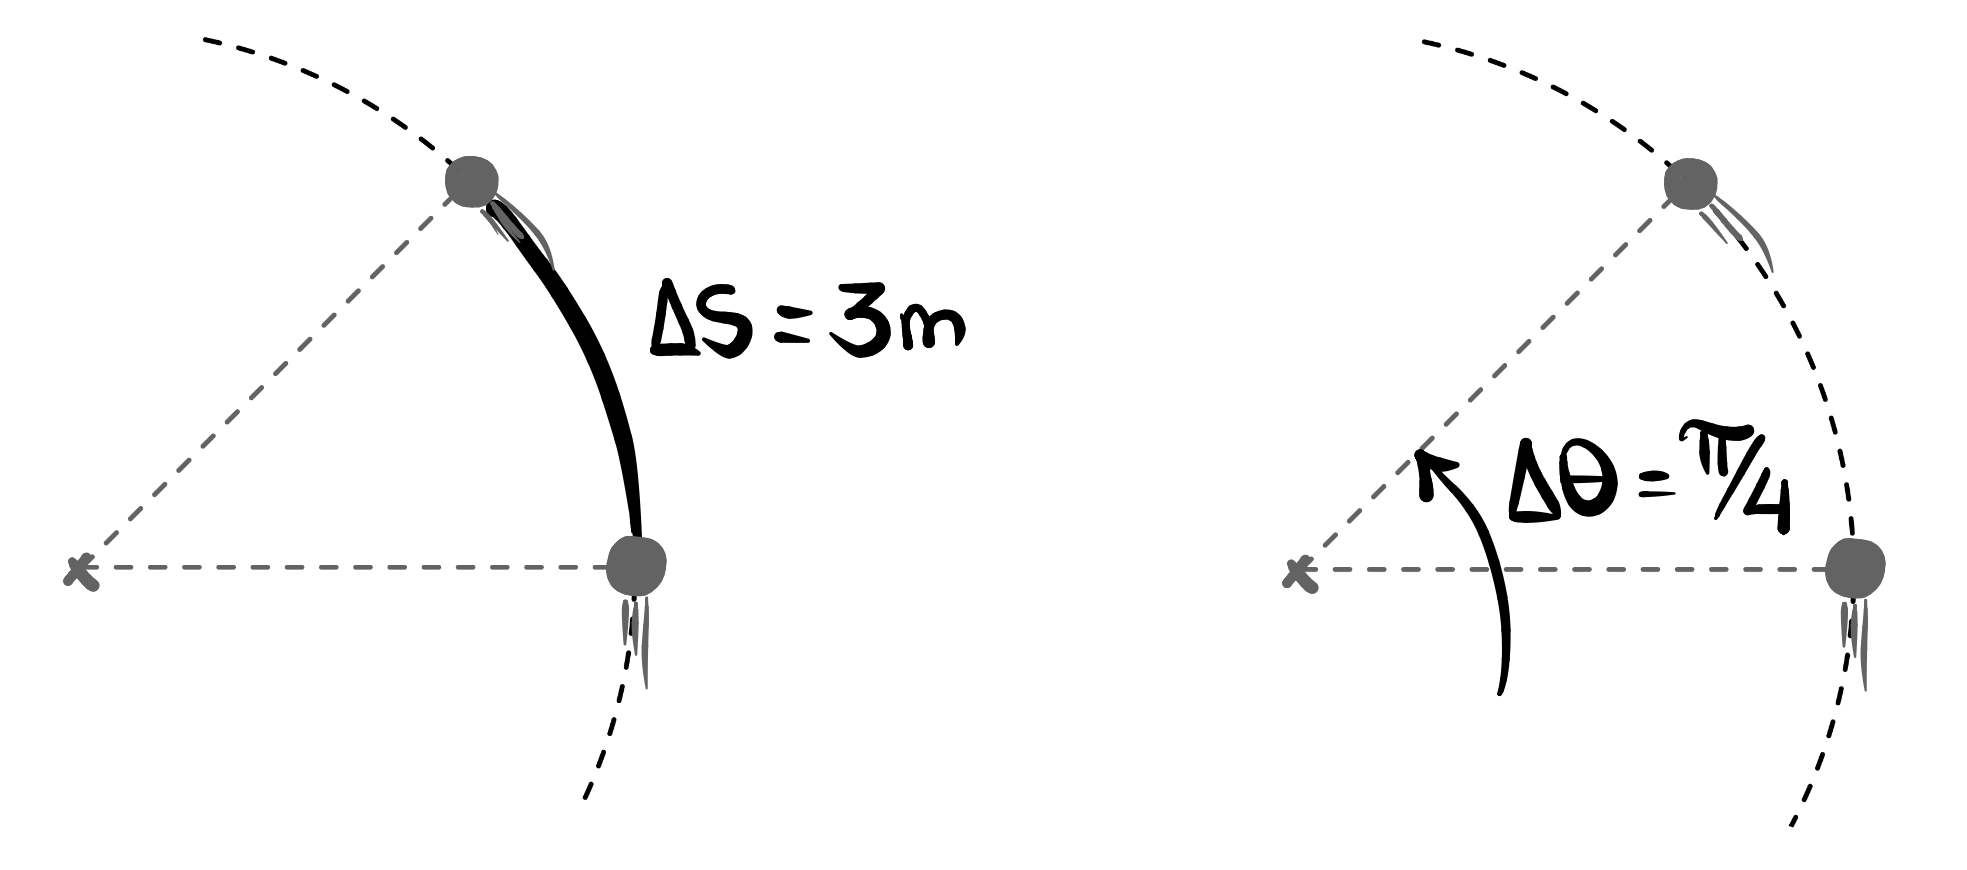
\includegraphics[width=0.6\linewidth]{imagenscinematicavetorial/deslocamentoangular.png}
\captionof{figure}{O deslocamento linear e angular.}
\label{fig_cinvet_deslocamentoangular}
} 
\vspace{0.3cm}


Dada uma circunferência, veja que existem duas formas equivalentes de se expressar o deslocamento de um corpo. No caso da Figura \ref{fig_cinvet_deslocamentoangular}, dizer que o corpo, em um certo intervalo de tempo, se deslocou 3 metros; ou dizer que ele se deslocou 45 graus, ou seja, $\sfrac{\pi}{4}$ radianos, são informações equivalentes. Das duas formas conseguimos, dada uma posição inicial, descobrir onde o corpo estará no próximo instante de tempo, ou seja, nos permitem fazer uma descrição cinemática do movimento do corpo.

Sendo assim, podemos criar uma grandeza angular análoga à velocidade média definida na Equação \eqref{mecanica_eq_velocidademedia}. Ora, se lá definimos a velocidade linear\footnote{Para diferenciar as grandezas, o que já conhecíamos como velocidade, será aqui chamada de velocidade linear. Trata-se da mesma grandeza até então conhecida por nós -- é uma acréscimo de vocabulário apenas para certificar de que vamos conseguir diferenciar com clareza $v$ de $\omega$, isto é, a velocidade linear da velocidade angular.} $v$ como sendo a razão entre o deslocamento linear $\Delta s$ pelo intervalo de tempo; é natural que se defina a velocidade angular $\omega$ como sendo a razão entre o deslocamento angular $\Delta \theta$ e o intervalo de tempo, que é justamente o que aparece na Equação \eqref{cinvet_eq_velangular}.

Perceba que, enquanto a velocidade linear $v$ mede o quão rápido se percorre uma distância, ou seja, quantos metros se percorre por segundo; a velocidade angular $\omega$ mede o quão rápido se percorre um ângulo, ou seja, quantos radianos se gira por segundo, por exemplo.



\secgfe{Onde é usada}

Em quaisquer problemas que envolvam movimentos periódicos, em particular, para movimentos circulares.


\secgfe{Erros comuns}

O erro mais comum aqui é o estudante querer usar os ângulos em graus e não em radianos. Isso, eventualmente, pode levá-lo a alguns erros, que estarão relacionados à natureza geométrica da definição de radiano. Na seção em que apresentaremos a Equação \eqref{cinvet_eq_velangularelinear} vamos discutir em detalhes este fato e ficará claro por qual razão é mais natural usar radianos e não graus. Por hora, fica a ressalva ao leitor: o ideal que todos os ângulos, em equações físicas, sejam calculados e inseridos em radianos.

Desse modo, a unidade padrão no S.I. para velocidade angular é o rad/s.


\secgfe{Observações}

O contexto mais comum em que aplicaremos a Equação \eqref{cinvet_eq_velangular} será o de movimentos circulares, em particular, o movimento circular uniforme (MCU). Em tal contexto, a velocidade angular $\omega$, por ser constante, será igual à velocidade angular média $\omega_m$ em qualquer intervalo de tempo, ou seja

$$ \omega_m = \omega = \dfrac{\Delta \theta}{\Delta t}.$$

No intervalo de tempo de um período $T$, o ângulo total girado será o de uma volta, isto é, $\Delta \theta = 2\pi$ rad, logo, teremos

$$ \omega =  \dfrac{\Delta \theta}{\Delta t} = \dfrac{2 \pi}{T} \implies \boxed{\omega =  \dfrac{2 \pi}{T} .}$$

Além disso, sendo a frequência o inverso do período, poderíamos escrever a equação acima como

$$ \omega = \dfrac{2 \pi}{T} = 2 \pi \cdot \dfrac{1}{T} = 2 \pi f \implies \boxed{\omega = 2 \pi f.}$$

As duas equações destacadas acima são apenas uma pequena variação da Equação \eqref{cinvet_eq_velangular}, \textbf{válidas exclusivamente para o MCU.} É comum que as usemos para resolver certos problemas, mas é importante que o leitor perceba que tais equações não são exatamente novas e sequer precisam ser memorizadas. São apenas um caso particular da própria definição de velocidade angular, aplicada ao MCU fixando o intervalo de tempo como sendo o de uma volta.

\vspace{0.3cm}


\begin{exemplo}[Nível I]\label{exemplo_cinvet_velocidadeangularex01}

Um ventilador realiza 120 rotações por minuto. Sendo a dimensão da sua pá de 15 cm, calcule a velocidade linear da extremidade da pá e sua velocidade angular.

\resolucao

A frequência é de 

$$\dfrac{120 \text{ rot.}}{1\text{ min}} = \dfrac{120 \text{ rot.}}{60 \text{ s}} = 2 s^{-1}.$$ 


Assim, a velocidade angular $\omega$ é

$$ \omega = \dfrac{\Delta \theta}{\Delta t} = \dfrac{2 \pi}{T} = 2 \pi \cdot \dfrac{1}{T} = 2 \pi f,$$

\noindent em que usamos que o ângulo total girado em um período é o de uma volta completa, isto é, $2 \pi $ rad, e que a frequência é o inverso do período. Substituindo os valores teremos

$$ \omega =2 \pi f =4 \pi\text{ rad/s} \approx 12 \text{ rad/s}.  $$

Já a velocidade linear $v$ é

$$ v = \dfrac{d}{t} = \dfrac{2 \pi R}{T} = 2 \pi R \cdot \dfrac{1}{T} = 2 \pi R f,$$

\noindent que, substituindo, fornece:

$$ v = 2 \pi R f = 2 \pi \cdot 0.15 \text{m} \cdot 2 s^{-1} = 0.6 \pi \text{ m/s} \approx 1.9 \text{ m/s}.$$

\end{exemplo}



\vspace{0.3cm}


\begin{exemplo}[Nível II]\label{exemplo_cinvet_velocidadeangularex02}

Um corpo descreve um movimento circular uniforme de raio $R$. Sua velocidade linear é $v$. Determine o tempo necessário para que ele descreva um ângulo de $5$ radianos.


\resolucao

Usando a definição de velocidade angular, temos

$$ \omega = \dfrac{\Delta \theta}{\Delta t} = \dfrac{5}{\Delta t} \implies \Delta t = \dfrac{5}{\omega}.$$

Sendo assim, o problema consiste em encontrar a velocidade angular $\omega$ da partícula.

Sabemos sua velocidade linear $v$ e o raio $R$ da circunferência. Com isso, temos

$$ v = \dfrac{d}{t}=\dfrac{2 \pi R}{T} = \underbrace{\dfrac{2 \pi}{T}}_{\substack{\text{velocidade}\\\text{angular}}}\cdot R = \omega R \implies \omega = \dfrac{v}{R}.$$

Tal relação é tão importante que merece uma discussão à parte -- assunto para a próxima seção. Logo, tendo $\omega$ em termos dos parâmetros fornecidos, teremos o tempo pedido:

$$ \Delta t = \dfrac{5}{\omega} = \dfrac{5}{\sfrac{v}{R}} \implies \boxed{\Delta t = \dfrac{5R}{v} .} $$





\end{exemplo}





\begin{secnivel}[Relação entre $v$ e $\omega$.]{I}{Relação entre velocidade linear e angular}
  
  \eqLdois{dem}{cinvet_eq_velangularelinear}{v = \omega r}

\end{secnivel}






\secgfe{De onde vem}

A Equação \eqref{cinvet_eq_velangularelinear} mostra como podemos converter uma grandeza angular, como a velocidade angular $\omega$, no seu análogo linear, isto é, na velocidade linear $v:$ basta usar o raio $r$ de curvatura como fator de conversão.

Isso vem de um fato geométrico, relativo ao modo como definimos o radiano. Antes, lembremos como é definido um ângulo medido em graus: divida uma circunferência em 360 partes iguais. O ângulo de 1 grau é igual ao ângulo de abertura de uma dessas partes.

É por isso que uma volta completa tem $360^\circ$: por definição. Poderíamos muito bem ter escolhido dividir a circunferência em 120 partes iguais -- ou até mesmo em 100 partes iguais, dado o fato de que usamos um sistema decimal e tudo funciona de dez em dez. O fato de que o grau é definido como sendo uma parte em 360 da circunferência é herança dos babilônios, que usavam um sistema sexagesimal (base 60), mas não vamos entrar em grandes detalhes nisso. 


\vspace{0.3cm}
{
\centering
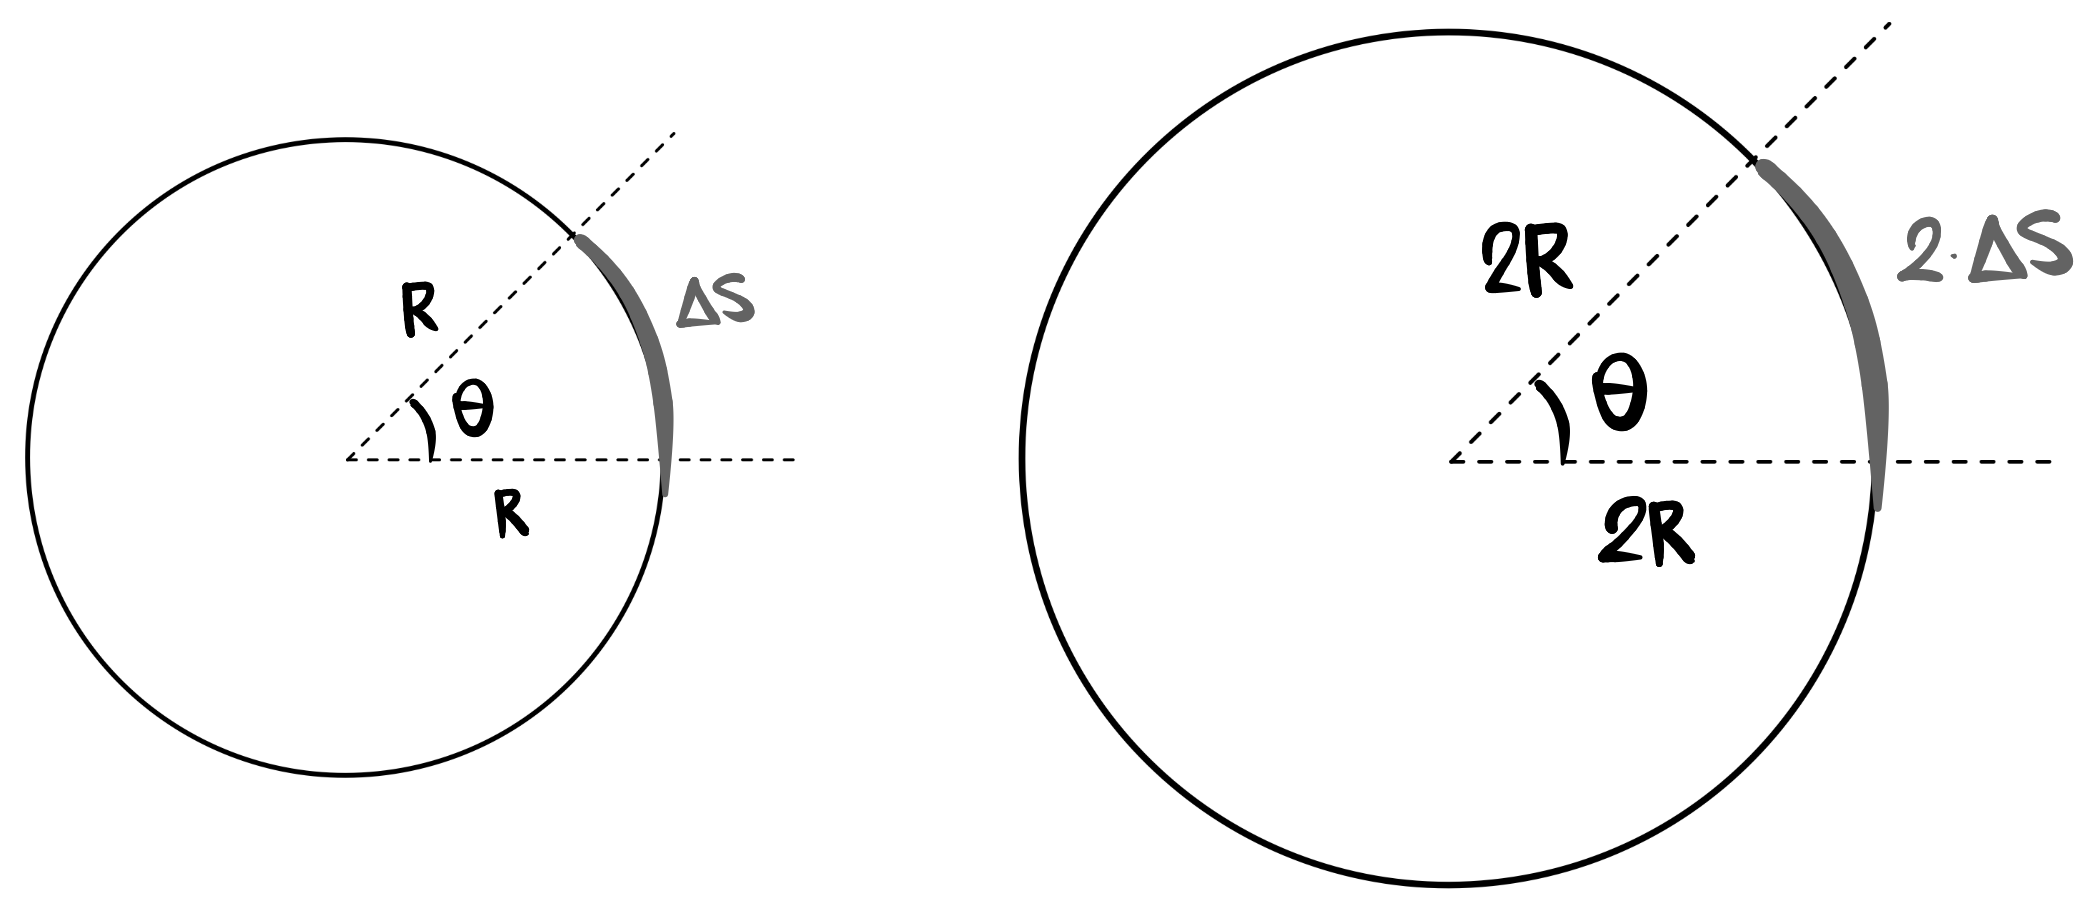
\includegraphics[width=0.5\linewidth]{imagenscinematicavetorial/definicaoradiano1.png}
\captionof{figure}{A unidade de medida natural para ângulos consiste em usar o próprio raio da circunferência como unidade de medida.}
\label{fig_cinvet_defradiano1}
} 

\vspace{0.3cm}

O fato é que existe uma outra forma de se definir a medida de ângulos -- uma forma bem menos artificial, diga-se de passagem. Tal maneira consiste em se usar o próprio raio da circunferência como unidade de medida: um ângulo $\theta$ em radianos é definido como sendo a razão entre o comprimento $\Delta s$ do arco de circunferência que ele subentende e o raio da circunferência $R$:

$$ \theta := \dfrac{\Delta s}{R}.$$





A Figura \ref{fig_cinvet_defradiano1} ilustra o fato de que, ao definir o ângulo dessa forma, a medida do ângulo independe da circunferência que usamos para medi-lo. Isso porque, avaliando a mesma abertura angular em uma circunferência que tenha o dobro do raio, vemos que, por ter o dobro do raio, o arco de circunferência referente à mesma abertura angular terá o dobro de comprimento, de modo que a razão entre essas duas grandezas será a mesma:

$$ \theta = \dfrac{\Delta s}{R} = \dfrac{2 \Delta s}{2R},$$


\noindent ou seja, independente da circunferência que se use, medindo o ângulo dessa forma seremos sempre levados ao mesmo valor.


Essa é, portanto, a forma mais natural de se medir o ângulo: usando como régua de medida o próprio raio da circunferência -- e já vimos que isso nos leva a uma medida angular que independe do raio da circunferência, ou seja, trata-se de uma medida, de certo modo, absoluta (e não relativa a uma circunferência específica). Note que tal forma de medir nos leva a um número adimensional: a razão entre dois comprimentos, $\Delta s$ e $R,$ respectivamente. 

Assim, o ângulo de uma unidade nesse sistema significaria uma abertura angular tal que o comprimento de arco na circunferência referente a tal abertura fosse de exatamente um raio. Um ângulo de duas unidades, por sua vez, representaria uma abertura angular tal que o comprimento de arco na circunferência referente a tal abertura fosse de exatamente dois raios. A Figura \ref{fig_cinvet_defradiano2} ilustra essas situações, mostrando que, para um ângulo de 3 unidades, isto é, uma abertura angular que enxerga um arco de três raios de comprimento, teremos varrido quase meia circunferência.


\vspace{0.3cm}
{
\centering
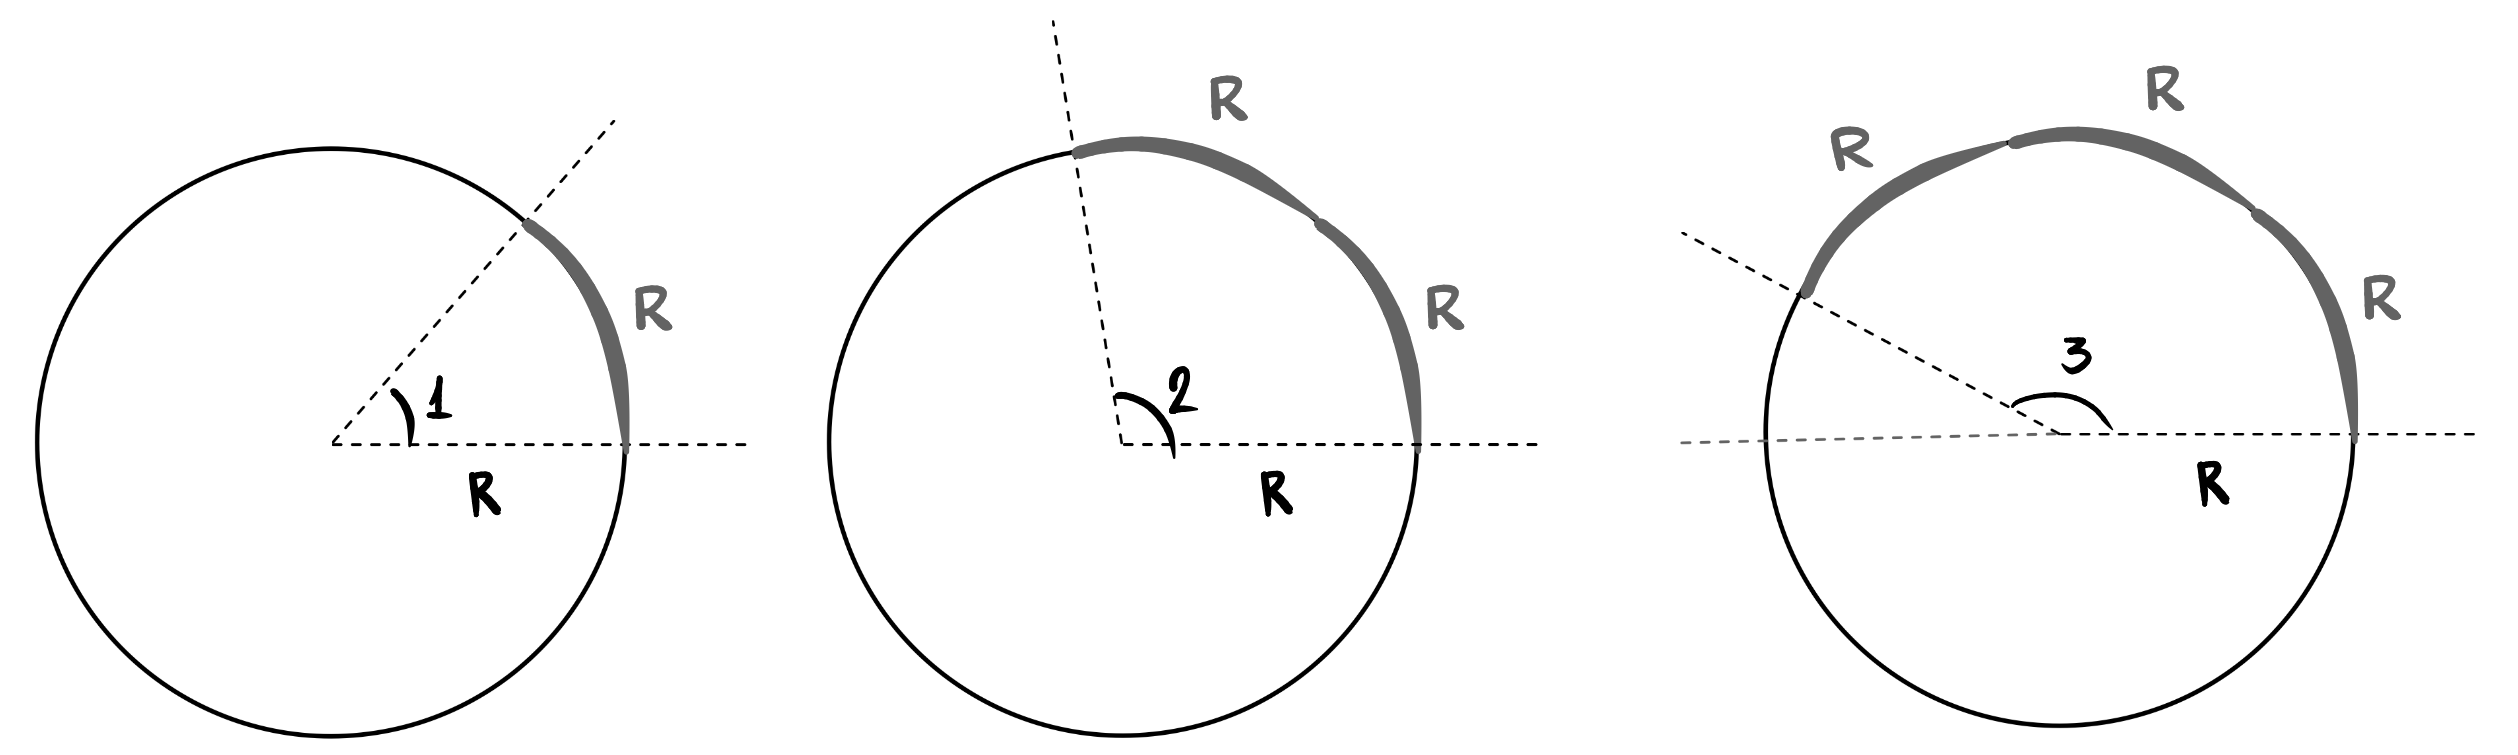
\includegraphics[width=0.8\linewidth]{imagenscinematicavetorial/definicaoradiano2.png}
\captionof{figure}{Alguns ângulos em radianos.}
\label{fig_cinvet_defradiano2}
} 

\vspace{0.3cm}
Para varrer exatamente meia circunferência precisaríamos na verdade de um ângulo de medida $\pi \approx 3,14$, ou seja, um ângulo que enxerga um arco de circunferência de 3,14 raios de comprimento. É fácil notar isso, uma vez que sabemos o comprimento de uma circunferência completa, de modo que o ângulo de uma volta completa é de

$$ \theta = \dfrac{\Delta s}{R} = \dfrac{2 \pi R}{R} = 2 \pi,$$

\noindent e, portanto, o ângulo de meia volta é de $\pi \approx 3,14$.


Para não deixar ambiguidade em relação a essa forma de medir ângulos, damos a ela um nome: radiano. Isso é só para que não haja confusão quando alguém te disser algo como \textit{considere um ângulo de medida 2...}

Ora, 2 o quê? 2 graus? Ou seria um ângulo tal que ele enxerga um arco de circunferência de comprimento igual a 2 raios? Por ser adimensional, essa nova unidade de medida pode gerar esse tipo de dúvida, de modo que damos a ela o nome de radiano: a abertura angular tal que o comprimento de arco na circunferência referente a tal abertura é de exatamente dois raios tem medida de 2 radianos. 

É importante notar, porém, que para o ângulo de $2$ rad, o termo rad não é exatamente uma unidade de medida -- o ângulo medido dessa forma é, na verdade, adimensional, por ser uma razão entre dois comprimentos. Assim, o rad é apenas um nome que conectamos com o número para eliminar algum tipo de dúvida em relação a qual é a forma que está sendo usada para medir ângulos (alguns autores chamam isso de \emph{unidade auxiliar}.)

Talvez o leitor pense que todo esse devaneio -- puramente matemático -- a respeito do que é um radiano não tenha nada a ver com a física em questão e seja mero preciosismo. Vejamos agora que, na verdade, a Equação \eqref{cinvet_eq_velangularelinear} é simplesmente uma consequência direta da forma como define-se o radiano. De tal definição -- usando agora $\Delta \theta$ para representar a abertura angular no lugar de apenas $\theta$ -- temos que 

$$ \Delta s = \Delta \theta R,$$

\noindent ou seja, se temos uma grandeza angular, $\Delta \theta$, e queremos achar seu correspondente linear, $\Delta s$, fazemos isso simplesmente multiplicando aquela pelo raio $R$ da circunferência: assim, convertemos a abertura angular em abertura linear (comprimento do arco).

Agora, considere que essa abertura angular é gerada por uma partícula que executa um MCU ao longo dessa circunferência. Assim, dividindo a equação acima por $\Delta t$, teremos:


$$ \underbrace{\Delta s = \Delta \theta R}_{\text{definição de radiano}} \xrightarrow{\text{dividindo por $\Delta t$}}  \underbrace{\dfrac{\Delta s}{\Delta t}}_{v} = \underbrace{\dfrac{\Delta \theta}{\Delta t}}_{\omega} R, $$


\noindent de onde segue naturalmente que $v=\omega R,$ que é o que queríamos provar. Perceba, portanto, que tal equação só vale se usarmos a medida angular em radianos, uma vez que a Equação \eqref{cinvet_eq_velangularelinear} é, em sua essência, a própria definição de radianos, porém considerando a variação no tempo. Vale lembrar também que as razões $\sfrac{\Delta s}{\Delta t}$ e $\sfrac{\Delta \theta}{\Delta t}$ só coincidem com os valores das velocidades linear $v$ e angular $\omega$, respectivamente, para o movimento uniforme. Do contrário tais razões forneceriam as velocidades lineares e angulares médias, respectivamente.

\secgfe{Onde é usada}

Tal equação pode ser usada basicamente em qualquer contexto em que haja um MCU. Contudo, uma aplicação muito comum dela é para o estudo de problemas nos quais dois corpos estão executando um certo tipo de movimento circular, porém com algum nível de acoplamento. Por exemplo, quando estamos andando de bicicleta: existe uma correia que transmite o movimento de giro do pedal para uma catraca na roda de trás que, por sua vez, transmite a rotação para a roda traseira da bicicleta -- que é que faz o movimento ocorrer.

Veja que existem pelo menos 3 elementos girando na descrição acima, mas tais movimentos não são independentes: estão acoplados. Seja por uma correia ou por um eixo comum. A Equação \eqref{cinvet_eq_velangularelinear} costuma ser bastante útil para analisar contextos como esse, como veremos em alguns exemplos.



\secgfe{Erros comuns}

A Equação \eqref{cinvet_eq_velangularelinear} é relativamente simples, não deixando muitas margens para erro. O erro mais comum aqui é, provavelmente, em relação às unidades de medida. Vejamos como isso pode ocorrer.

Lembre-se de que, em se tratando da velocidade angular $\omega,$ definimos-a como sendo a razão entre o deslocamento angular $\Delta \theta$ e o intervalo de tempo $\Delta t$. Contudo, o ângulo em radiano -- a unidade natural para medir ângulos -- é adimensional. Logo, a unidade de medida de velocidade angular pode ser entendida como sendo 
 $$\dfrac{\text{rad}}{\text{s}},$$ 

\noindent ou, simplesmente, 

$$\dfrac{1}{\text{s}}=\text{s}^{-1},$$

\noindent haja vista que radiano é apenas um nome que damos para uma medição de ângulo que é intrinsecamente adimensional.

Assim, a velocidade angular $\omega$ é, de forma intrínseca, uma frequência. Ambas as grandezas têm dimensão $\text{s}^{-1}$, e é por isso que $\omega$ costuma ser chamada de \textit{frequência angular}. Contudo, elas não são a mesma grandeza: $f$ conta ciclos por segundo (unidade: Hz), enquanto $\omega$ conta radianos por segundo (unidade: rad/s). A diferença é justamente o fator $2\pi$ da equação $\omega = 2\pi f$ anteriormente construída por nós, que converte ciclos em radianos.

% Note que a equação $\omega = 2 \pi f$, construída na seção anterior, contém essa informação: sendo $2\pi$ uma constante e tendo que ser iguais as unidades de medida do lado esquerdo e direito de uma equação física, concluímos que a unidade de medida de $\omega$ é a mesma unidade de medida de $f$. Na verdade, $\omega$ é simplesmente a frequência $f$ multiplicada por um fator constante, logo, é natural que se trate também de uma frequência. Usamos, contudo, o Hertz (Hz) para medir a frequência $f$, enquanto a medida da frequência angular se dá em rad/s: a diferença entre as duas se dá pelo fator $2 \pi$ na equação $\omega = 2 \pi f.$

Perceba que tudo isso só faz sentido se usamos a medida do deslocamento angular $\Delta \theta$ em radianos, que é, na verdade, uma unidade de medida adimensional. Tudo isso para dizer que, para que possamos usar diversas equações, como por exemplo, $\omega = 2 \pi f$, é imprescindível que usemos $\Delta \theta$ em radianos no cálculo de $\omega.$

O erro mais comum aqui é o estudante usar $\omega$ em outra unidade de medida, como por exemplo $\text{graus}/\text{s}$, o que incorrerá certamente em erros ao longo do desenvolvimento.


Por fim, lembre-se que, no S.I., a unidade de medida para velocidade $v$ é $\text{m}\text{s}^{-1},$ e a unidade de medida da velocidade angular $\omega$ é $\text{s}^{-1}.$ Assim, usando o raio $R$ em metros, as unidades de medida dos dois lados da Equação \eqref{cinvet_eq_velangularelinear} ficam iguais, mantendo a coerência necessária. Ou seja, novamente vemos que uma exigência para que a Equação \eqref{cinvet_eq_velangularelinear} possa ser usada é que se use a velocidade angular $\omega$ com o ângulo sendo medido em radianos.


\secgfe{Observações}

Uma observação interessante é que a partir da Equação \eqref{cinvet_eq_velangularelinear} é possível obter diversas outras que construímos anteriormente. Usando, por exemplo, que $\omega = \sfrac{2 \pi}{T},$ chegamos em

$$  v = \omega R \implies v = \dfrac{2 \pi R}{T},$$

\noindent e, usando que a frequência é o inverso do período, chegamos em

$$ \boxed{v = 2 \pi R f.}$$

Um outro exemplo seria usarmos diretamente a equação acima na Equação \eqref{cinvet_eq_velangularelinear}:


$$  v = \omega R \implies 2 \pi R f = \omega R \implies \boxed{\omega = 2 \pi f.}$$


\vspace{0.3cm}


\begin{exemplo}[Nível I]\label{exemplo_cinvet_velocidadeangularelinearex01}

Considere as duas massas $A$ e $B,$ conectadas por um bastão rígido, que gira em torno do ponto $O.$ Se a distância entre $A$ e $B$ é a mesma entre $B$ e $O,$ qual é a relação entre as velocidades lineares de $A$ e $B?$

\resolucao

A Figura \ref{fig_cinvet_v=wr exemplo01} ilustra a situação do problema. A parte mais importante -- que cabe à interpretação do estudante -- é perceber que, neste contexto, as duas bolinhas executam um MCU acoplado, de tal forma que a velocidade angular $\omega$ delas é a mesma. 



\vspace{0.3cm}
{
\centering
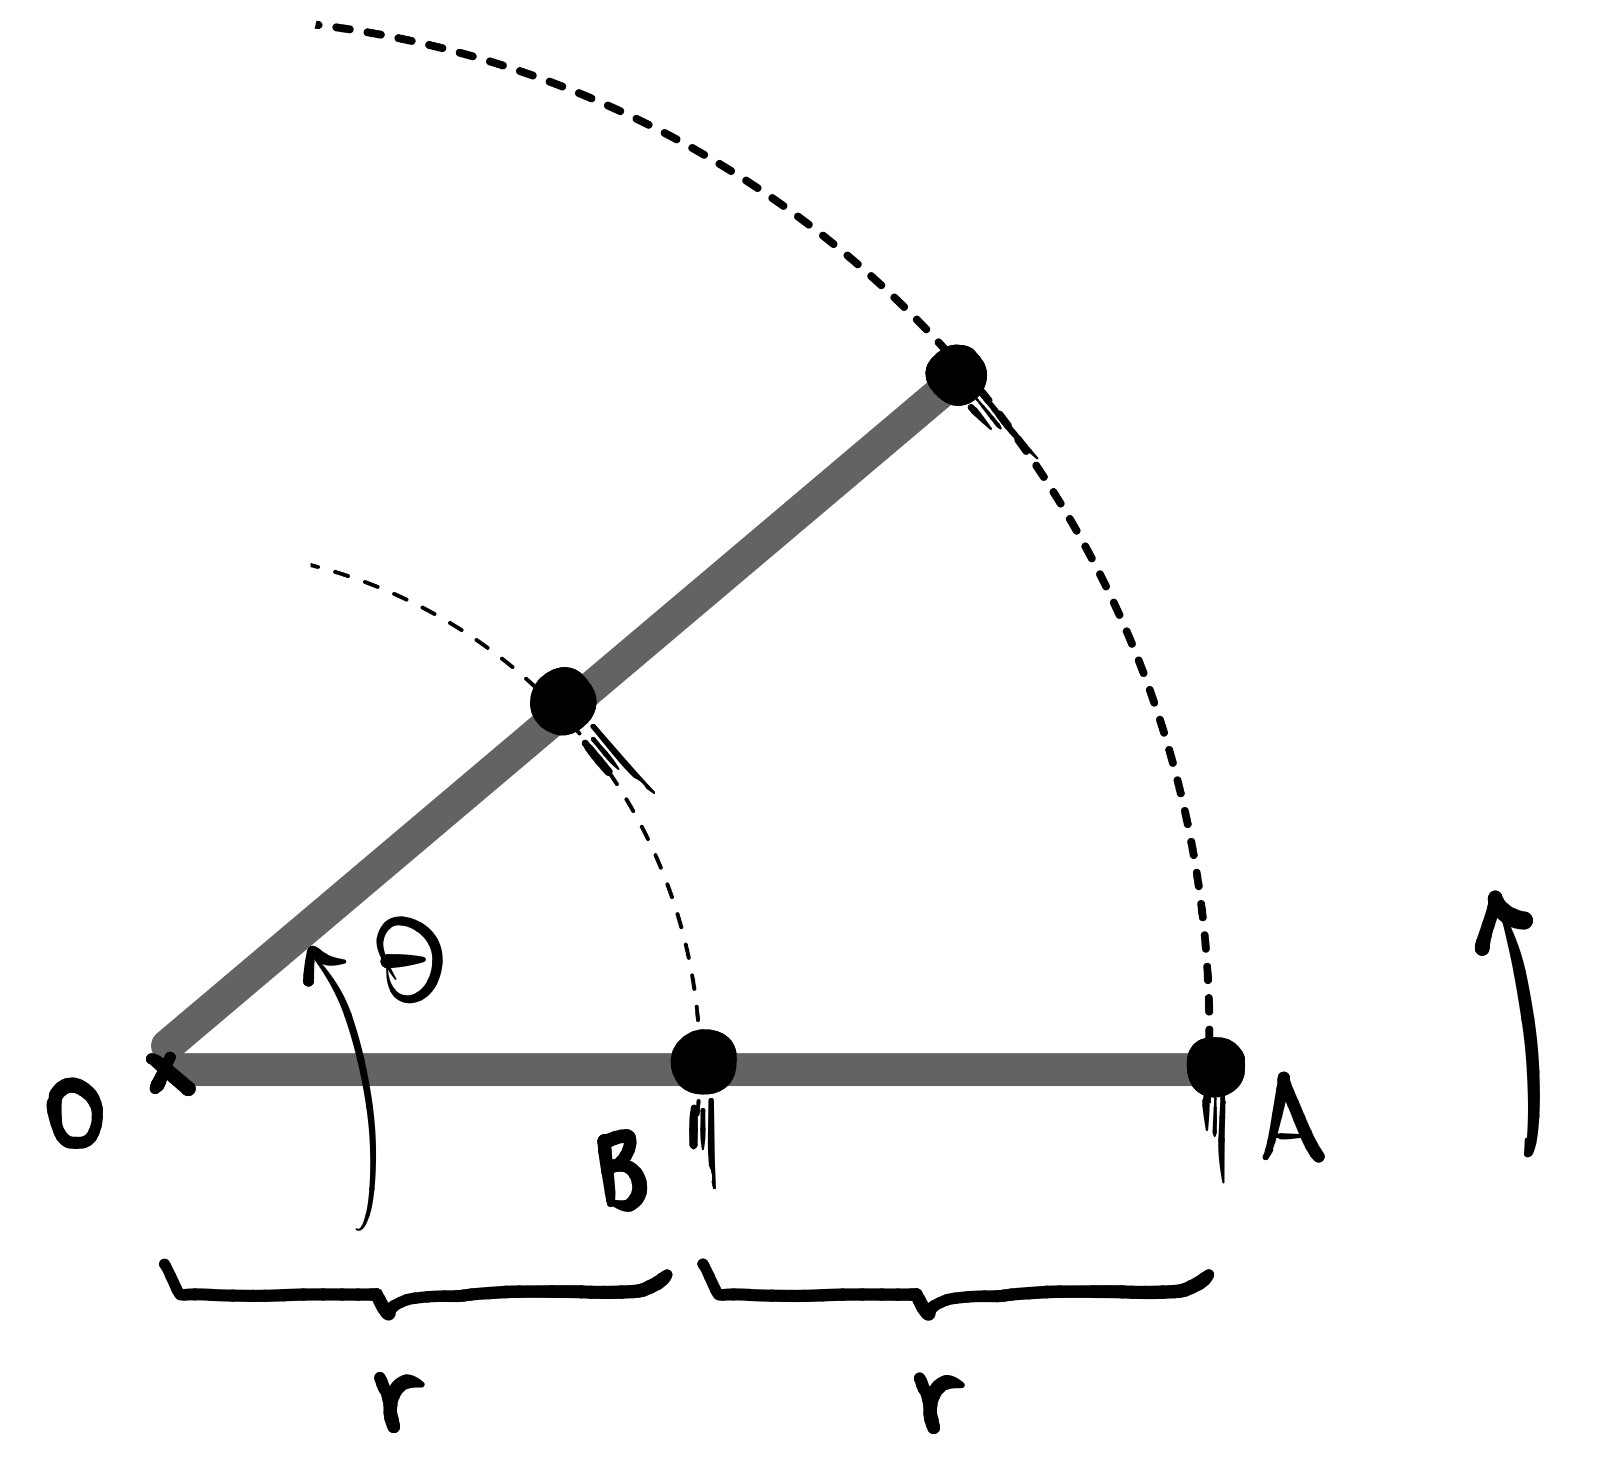
\includegraphics[width=0.35\linewidth]{imagenscinematicavetorial/v=wr exemplo01.png}
\captionof{figure}{}
\label{fig_cinvet_v=wr exemplo01}
} 

\vspace{0.3cm}

A figura tenta evidenciar isso, mostrando que, quando uma delas gira um certo ângulo $\theta,$ a outra, por estar fixa por uma haste rígida à primeira, obrigatoriamente gira, também, o mesmo ângulo. Logo, neste caso, podemos escrever que

$$ \omega_A = \omega_B \implies \dfrac{v_A}{R_A} = \dfrac{v_B}{R_B} \implies \dfrac{v_A}{2r} = \dfrac{v_B}{r} \implies \boxed{v_A = 2 v_B.}$$

Perceba que essa mesma conclusão poderia ter sido tirada sem o uso de equações: sendo o raio da circunferência $A$ o dobro do raio da circunferência $B,$ concluímos que o comprimento total da circunferência $A$ é o dobro do comprimento da circunferência $B.$ Logo, como as hastes giram juntas, quando $A$ completar uma volta, $B$ também terá completado uma volta, de modo que o período delas é o mesmo. Porém, tendo que varrer o dobro de distância no mesmo tempo, a velocidade linear de $A$ deve ser o dobro da de $B.$ \\

De certo modo, toda essa análise é capturada pelo tratamento matemático que fizemos ao usar $v = \omega r.$ Contudo, é importante entender o que se passa por trás dos processos algébricos ao manipular equações.

\end{exemplo}



\vspace{0.3cm}



\begin{exemplo}[Nível II]\label{exemplo_cinvet_velocidadeangularelinearex02}

Considere um ciclista que dá 2 pedaladas por segundo (cada pedalada significa realizar uma volta completa no disco acoplado aos pedais).

Se o raio do disco acoplado aos pedais é de 4cm, o raio da roda traseira é de 32 cm e o raio da catraca traseira -- que está acoplado por uma correia ao disco dos pedais -- é de 8 cm, qual é a velocidade com que o ciclista se move?

\resolucao

Sejam $A$, $B$ e $C$ o disco acoplado aos pedais, a catraca e a roda traseira, respectivamente. E sejam $R_A,$ $R_B,$ e $R_C$ os seus raios, respectivamente.


\vspace{0.3cm}
{
\centering
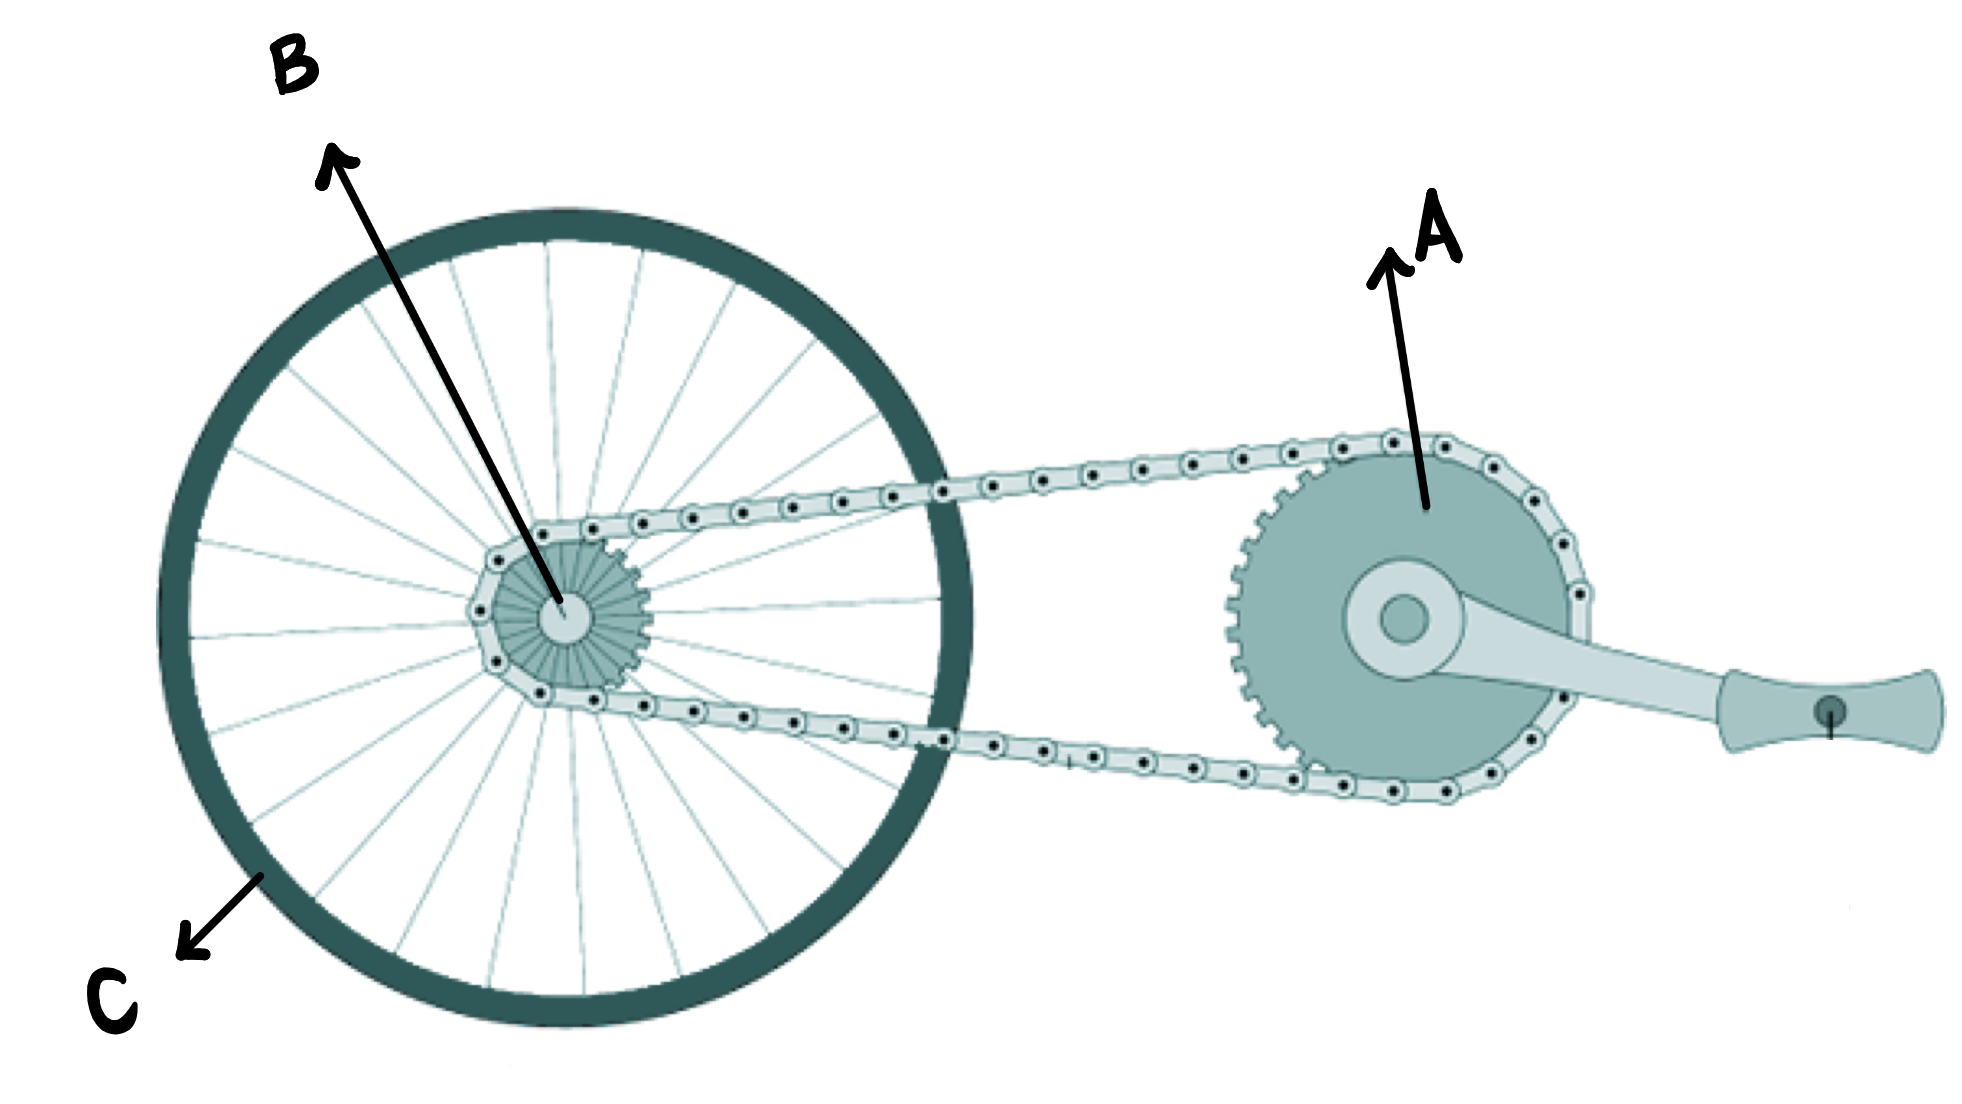
\includegraphics[width=0.5\linewidth]{imagenscinematicavetorial/bicicleta.png}
\captionof{figure}{}
\label{fig_cinvet_bicicelta}
} 

\vspace{0.3cm}


Como mostra Figura \ref{fig_cinvet_bicicelta}, a transmissão de movimento do disco acoplado aos pedais para a catraca se dá através de uma correia, que transmite a velocidade de um disco para o outro. Sendo a velocidade linear de todos os pontos da correia sempre a mesma, isso gera um acoplamento que obriga esses dois discos a girarem com mesma velocidade linear, ou seja:

$$ v_A = v_B \implies \omega_A R_A = \omega_BR_B \implies \omega_B = \omega_A\dfrac{R_A}{R_B}.$$


Já a catraca $B$ e a roda traseira $C$ giram sob um mesmo eixo, o que vem a ser o mesmo caso do exemplo anterior. Logo, elas possuem a mesma velocidade angular:

$$ \omega_B = \omega_C \implies  \omega_A \dfrac{R_A}{R_B} = \dfrac{v_C}{R_C} \implies v_C = \omega_A  \dfrac{R_A R_C}{R_B},$$

\noindent ou seja, para descobrir a velocidade da bicicleta $v_C$ -- que será igual à velocidade de movimento da sua roda traseira -- basta descobrir o valor da frequência angular $\omega_A$ de giro dos pedais. Ora, temos a informação de que o ciclista dá duas pedaladas por segundo, ou seja, o disco $A$ dá duas voltas por segundo: $f_A = 2$Hz. Logo, usando que $\omega = 2 \pi f,$ temos:

$$ \omega_A = 2 \pi f_A = 4 \pi \text{ Hz},$$

\noindent de modo que a velocidade $v_C$ da bicicleta é

$$ v_C = \omega_A  \dfrac{R_A R_C}{R_B} = 4 \pi \dfrac{0,04 \cdot 0,32}{0,08}  \approx 2 \text{ m/s.} $$

Note que convertemos os raios para metros, a fim de obter a resposta final em m/s.

\end{exemplo}







\paginailustracaoato{imagens_artes/newton.png}

\part{Dinâmica}
\epigrafeato{%
  O próximo grande passo no desenvolvimento de nossa compreensão
  do mundo foi este: as forças não são o que se precisa para
  produzir movimento; as forças são o que se precisa para
  produzir variações no movimento.%
}{Richard P. Feynman}



% !TeX spellcheck = pt_BR

\chapter*{Do que se trata a Dinâmica}
\addcontentsline{toc}{chapter}{Do que se trata a Dinâmica}

A Cinemática nos ensinou a descrever o movimento com precisão: como
dizer onde um corpo está, quão rápido vai, em que direção aponta sua
velocidade, como essa velocidade muda ao longo do tempo. É uma
linguagem poderosa --- e, como toda boa linguagem, deliberadamente
incompleta. Ela descreve \textit{o quê}, mas se recusa, por princípio,
a responder \textit{por quê.}

É exatamente essa pergunta que a Dinâmica se propõe a responder.

O conceito central é o de \textbf{força} --- e, com ele, uma ruptura
que levou quase dois mil anos para acontecer. Durante esse tempo, o
mundo acreditou em Aristóteles: a força seria a causa do movimento.
Para um corpo se mover, seria necessário que uma força agisse
continuamente sobre ele. Intuitivo e razoável, porém equivocado.

Foi Galileu quem percebeu a falácia, ao observar bolinhas deslizando
em planos inclinados perfeitamente lisos. Foi Newton quem a
formalizou, ao enunciar que a força não é a causa do movimento, mas
a causa da \textit{variação} do movimento --- da aceleração. Um corpo
em repouso permanece em repouso sem precisar de nenhuma força para
isso. Um corpo em movimento permanece em movimento, na mesma direção
e com a mesma velocidade, enquanto nenhuma força resultante agir sobre
ele. O que exige força é a mudança.

Esse deslocamento conceitual --- de força como causa do movimento para
força como causa da aceleração --- é a virada mais importante de todo
este livro, e ela está no coração do Segundo Ato.

O nosso estudo se dividirá em duas partes. Na primeira, construiremos
a \textbf{Dinâmica Vetorial}: as Leis de Newton, a força gravitacional,
a força de atrito, o impulso, o momento linear e suas leis de
conservação. É uma linguagem inteiramente vetorial --- forças têm
direção e sentido, e tratá-las como escalares seria perder precisão
onde a precisão mais importa. O coração dessa parte são as Leis de Newton: uma estrutura lógica que descreve, a partir de grandezas vetoriais, as causas do movimento.

Na segunda parte, introduziremos uma linguagem complementar e
inteiramente escalar: a \textbf{Dinâmica Escalar}, baseada nos
conceitos de trabalho e energia. Essa formulação não substitui as
Leis de Newton --- descreve a mesma realidade física por um caminho
diferente, mais conveniente em situações onde o que importa não é
o que acontece \textit{durante} o percurso, mas o que muda entre o
estado inicial e o estado final do sistema.

As duas linguagens juntas --- vetorial e escalar --- formam o arsenal
completo da mecânica clássica. Com elas, estaremos prontos para o
Terceiro Ato: aplicar tudo que foi construído ao mundo real, dos
planetas em órbita ao comportamento dos fluidos.
% !TeX spellcheck = pt_BR


\chapter{Dinâmica -- Descrição Vetorial}



\section{Leis de Newton}



\begin{secnivel}[Segunda Lei de Newton]{I}{Segunda Lei de Newton}
  
  \eqLdois{def}{eq_dinamica1_segundaleinewton}{\vec{F}_R = m \vec{a}}

\end{secnivel}


Podemos entender a Segunda Lei de Newton como sendo a equação matemática por meio da qual se define o conceito de força: ela é definida em termos do efeito que ela produz sobre o corpo em que atua: variar o movimento desse corpo, isto é, gerar aceleração.\footnote{Esta é uma equação do tipo Definição, mas de uma natureza peculiar: ela não inventa um nome para algo que já observávamos, como fizemos com a velocidade média. Ela cria o próprio conceito de força — define o que a palavra significa em física, operacionalmente, em termos de efeitos mensuráveis. Assim, ao medir a massa de um objeto e sua aceleração, a força que nele atua é definida como sendo o produto dessas duas grandezas. O conteúdo físico profundo da mecânica newtoniana não está nessa equação sozinha, mas na combinação dela com as leis de força específicas que virão a seguir.}






\secgfe{De onde vem} \label{secao_mecanicanewtoniana_segundaleinewton}




Para começarmos a construir o entendimento sobre a Equação \eqref{eq_dinamica1_segundaleinewton} vamos divagar sobre o problema da Figura \ref{fig_dinamicanewton_f=ma1}: sabendo que a força para a direita é maior do que a força para a esquerda, para onde a caixa se move?


\vspace{0.3cm}
{
\centering
\begin{tikzpicture}
  \begin{scope}[blend mode=multiply]
    \node {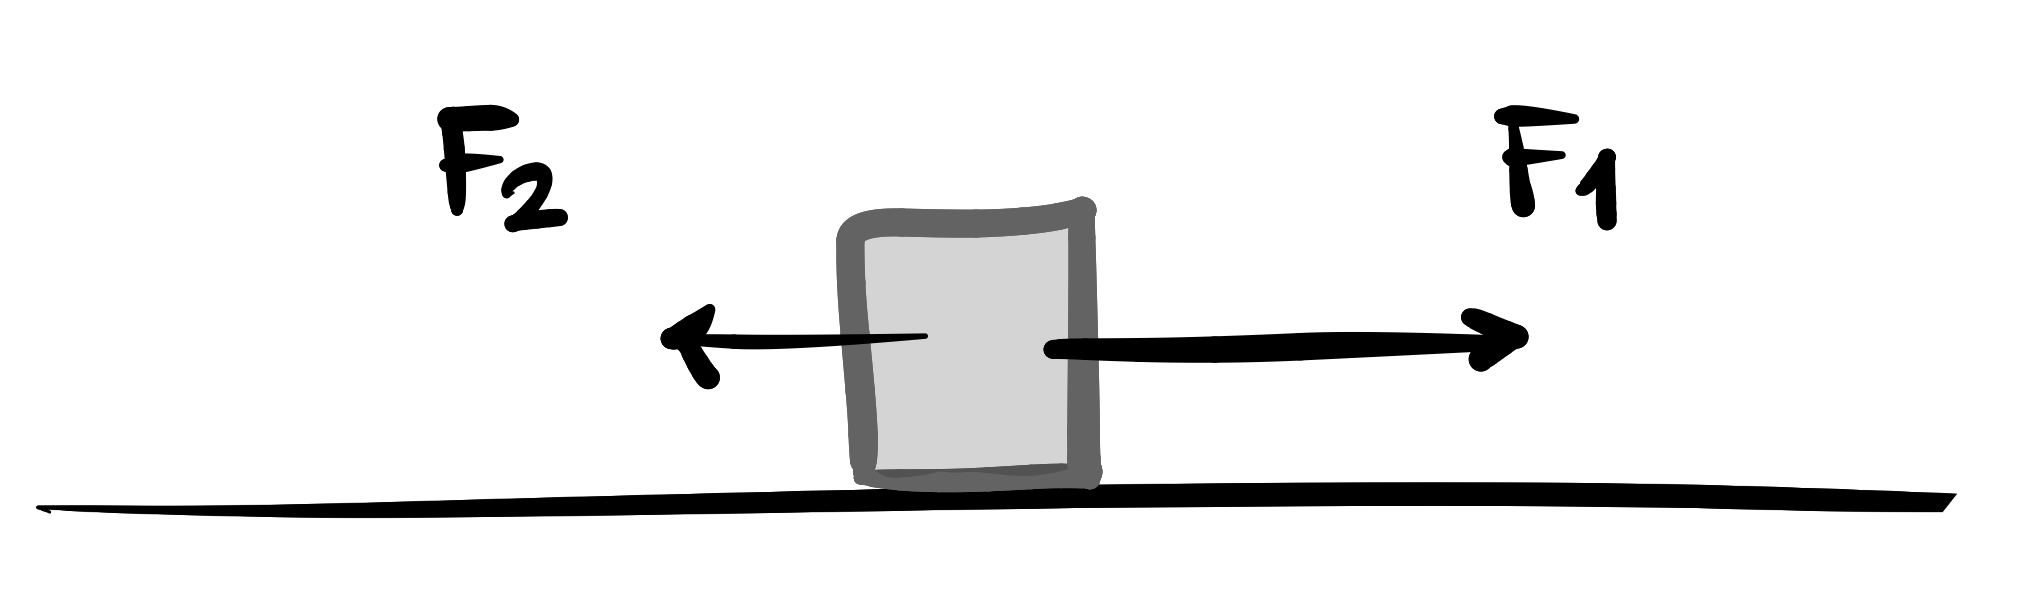
\includegraphics[width=0.4\linewidth]{imagensdinamicanewton/f=ma1.png}};
  \end{scope}
\end{tikzpicture}
\captionof{figure}{Se $F_1 > F_2$, para onde a caixa se move?}
\label{fig_dinamicanewton_f=ma1}
} 
\vspace{0.3cm}

Pelo senso comum, diríamos, com bastante segurança, que a caixa deve se mover para a direita. Razoável, não? Se você pensa assim, por ora, está tudo bem. Uma das mentes mais brilhantes da humanidade também pensava dessa forma -- o filósofo grego Aristóteles. Ocorre que tal conclusão está errada, e é isso que tentaremos perceber juntos a partir de agora.

Note que, ao responder que a caixa se move para a direita, a premissa da qual se parte é que a \textbf{força causa o movimento.} Ou seja, se a força para a direita é maior, então a caixa deve estar se movendo para a direita. Estamos partindo da noção de que existe uma relação de causalidade entre força e movimento. Lembrando que a velocidade é a grandeza física que definimos para medir movimento, estamos dizendo que a força é a causa da velocidade, isto é: a velocidade (ou seja, o movimento) se dá na mesma direção em que a resultante das forças atua:

$$ \boxed{\text{a força é necessária para que haja movimento.} }$$

Logo, se a força resultante for nula, o corpo estaria, segundo este raciocínio, em repouso. A Figura \ref{fig_dinamicanewton_f=ma2} ilustra algumas conclusões tiradas com o uso dessa linha de raciocínio: a caixa sempre se move na direção e no sentido para onde aponta a força resultante.

\vspace{0.3cm}
{
\centering
\begin{tikzpicture}
  \begin{scope}[blend mode=multiply]
    \node {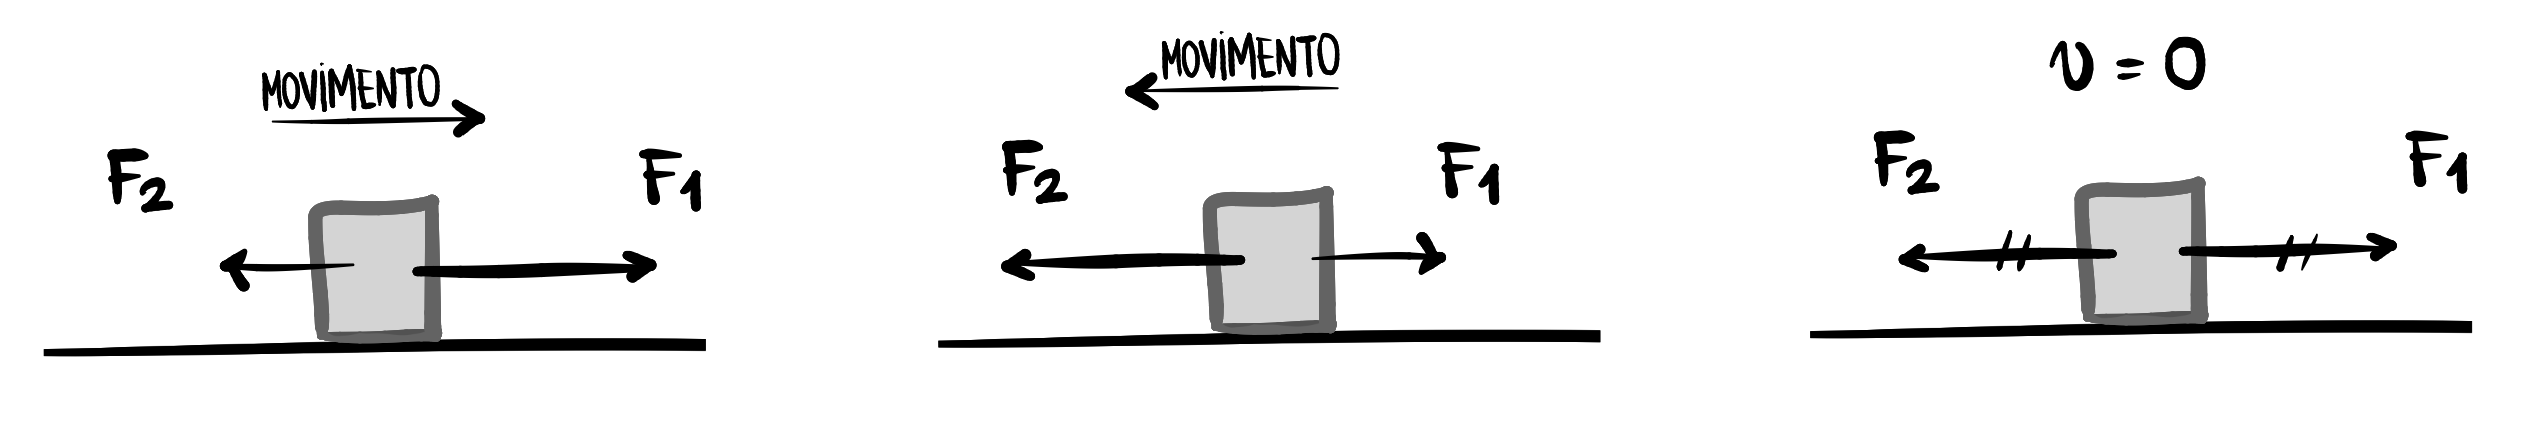
\includegraphics[width=0.9\linewidth]{imagensdinamicanewton/f=ma2.png}};
  \end{scope}
\end{tikzpicture}
\captionof{figure}{Segundo a visão aristotélica de movimento a caixa se moverá no mesmo sentido da força resultante. Se a força total for nula, o movimento (velocidade) da caixa será também nulo.}
\label{fig_dinamicanewton_f=ma2}
} 

\vspace{0.3cm}

Novamente, é importante destacar que tudo que conversamos até aqui é a visão de mundo aristotélica do movimento, e ela está equivocada, como veremos. É claro que tudo isso é bastante intuitivo e parece fazer sentido -- não em vão essa foi a visão de mundo durante quase dois mil anos, até que Galileu e Newton a sobrepujassem com uma nova teoria sobre o movimento. Contudo, se o mundo funcionasse apenas conforme nossa intuição, todo o campo de estudo da Física seria desnecessário. Ocorre que vários fenômenos são bem contraintuitivos e a natureza parece não gostar de funcionar da forma como achamos que ela deveria, e é do estudo dessa natureza aparentemente desobediente que cuida a Física.

Apenas para que o leitor consiga perceber a importância dessa teoria aristotélica do movimento , era a crença nela que incompatibilizou, durante séculos, a teoria de uma terra em movimento. A Figura \ref{fig_dinamicanewton_f=mamovimentoterra} irá nos ajudar a entender como. 

Suponha que a Terra tenha um movimento de rotação em torno do seu próprio eixo. Neste contexto, caso o menino pulasse -- como no ar não haveria nenhuma força que o mantivesse em movimento junto da terra -- ele acabaria ficando para trás, caindo em um ponto diferente do qual ele saltou.\footnote{A título de curiosidade, caso você ficasse por 1 segundo no ar durante este pulo -- o que é factível para um ser humano -- caso o leitor morasse no Pará, exatamente sob a linha do Equador, você ficaria para trás de uns 460 metros em relação ao ponto do qual pulou. Ou seja, com pouco menos de 100 pulos seria possível percorrer a distância do Pará ao Rio Grande do Sul: viajar do norte ao sul do Brasil, em poucos segundos.} Isso é claramente um absurdo e é só você dar um pulo agora onde está para se dar conta de que isso não ocorre.

\vspace{0.3cm}
{
\centering
\begin{tikzpicture}
  \begin{scope}[blend mode=multiply]
    \node {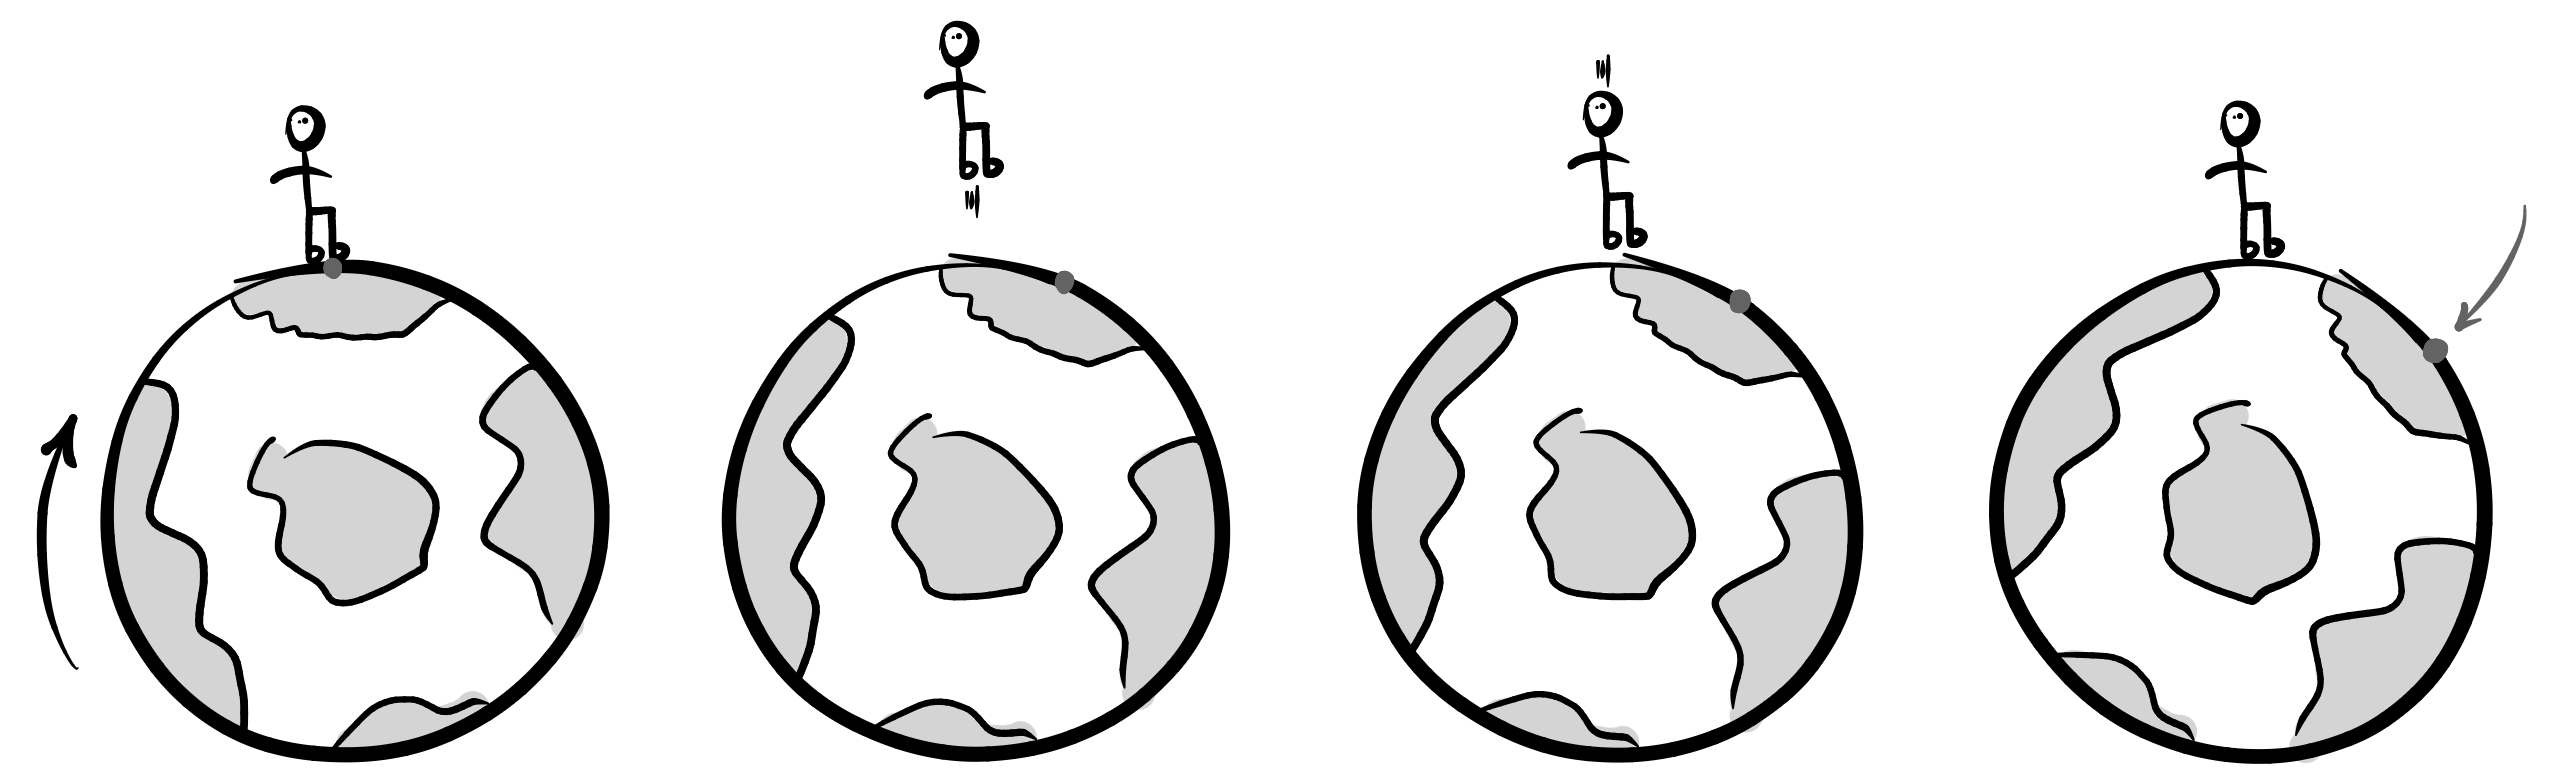
\includegraphics[width=0.8\linewidth]{imagensdinamicanewton/f=ma movimento terra.png}};
  \end{scope}
\end{tikzpicture}
\captionof{figure}{Se a força causa o movimento então uma cosmovisão em que a terra está em movimento é impossível.}
\label{fig_dinamicanewton_f=mamovimentoterra}
} 
\vspace{0.3cm}

O raciocínio, contudo, está impecável, e seguiria a própria lógica aristotélica de silogismos, partindo das premissas $P1,$ $P2$ e $P3,$ a conclusão é natural:

\begin{itemize}
    \item P1: A força causa o movimento.
    \item P2: Se a Terra se movesse, ao pular, no ar, sem contato com ela, não haveria nenhuma força que manteria o menino em movimento junto da Terra.
    \item P3: Logo, o menino iria cair em um ponto diferente daquele em que saltou.
    \item Conclusão: Como isso não ocorre, concluímos que a Terra não se move.
\end{itemize}

É por essas e por outras que levou-se quase dois mil anos para que uma teoria cosmológica em que a Terra estivesse em movimento ganhasse força. Foi apenas no século XVII que algumas teorias, como a de Copérnico, em que o Sol estava no centro e, portanto, a terra em movimento, começaram a se destacar. Isso ocorreu porque uma nova teoria mostrou que a premissa $P1$ estava errada: a força não causa o movimento. Foi Galileu -- um grande defensor do modelo cosmológico de Copérnico -- quem percebeu isso. Vejamos agora como.


Existe um experimento bastante conhecido de Galileu, chamado de experimento dos planos inclinados, que o levou à conclusão de que a força não é necessária para que haja movimento. A Figura \ref{fig_dinamicanewton_f=maplanoinclinado01} ilustra esse experimento: Galileu abandonava do repouso uma bolinha para escorregar ao longo de um plano inclinado, que estava conectado com um outro plano inclinado, todos bastante lisos e bem polidos. \footnote{A importância de deixar o plano bem polido é a de eliminar uma eventual força que pode se manifestar caso o chão não seja perfeitamente liso: a força de atrito. Queremos eliminar essa força justamente porque a intenção é entender o que ocorre com o movimento da bola na \textbf{ausência de forças}. Em breve estudaremos o atrito e entenderemos como ele afeta o movimento.} Ele observava, ao fazer o experimento, que por algum motivo que ele desconhecia a bolinha sempre chegava do outro lado exatamente na mesma altura: nem mais alto, nem mais baixo. 


\vspace{0.3cm}
{
\centering
\begin{tikzpicture}
  \begin{scope}[blend mode=multiply]
    \node {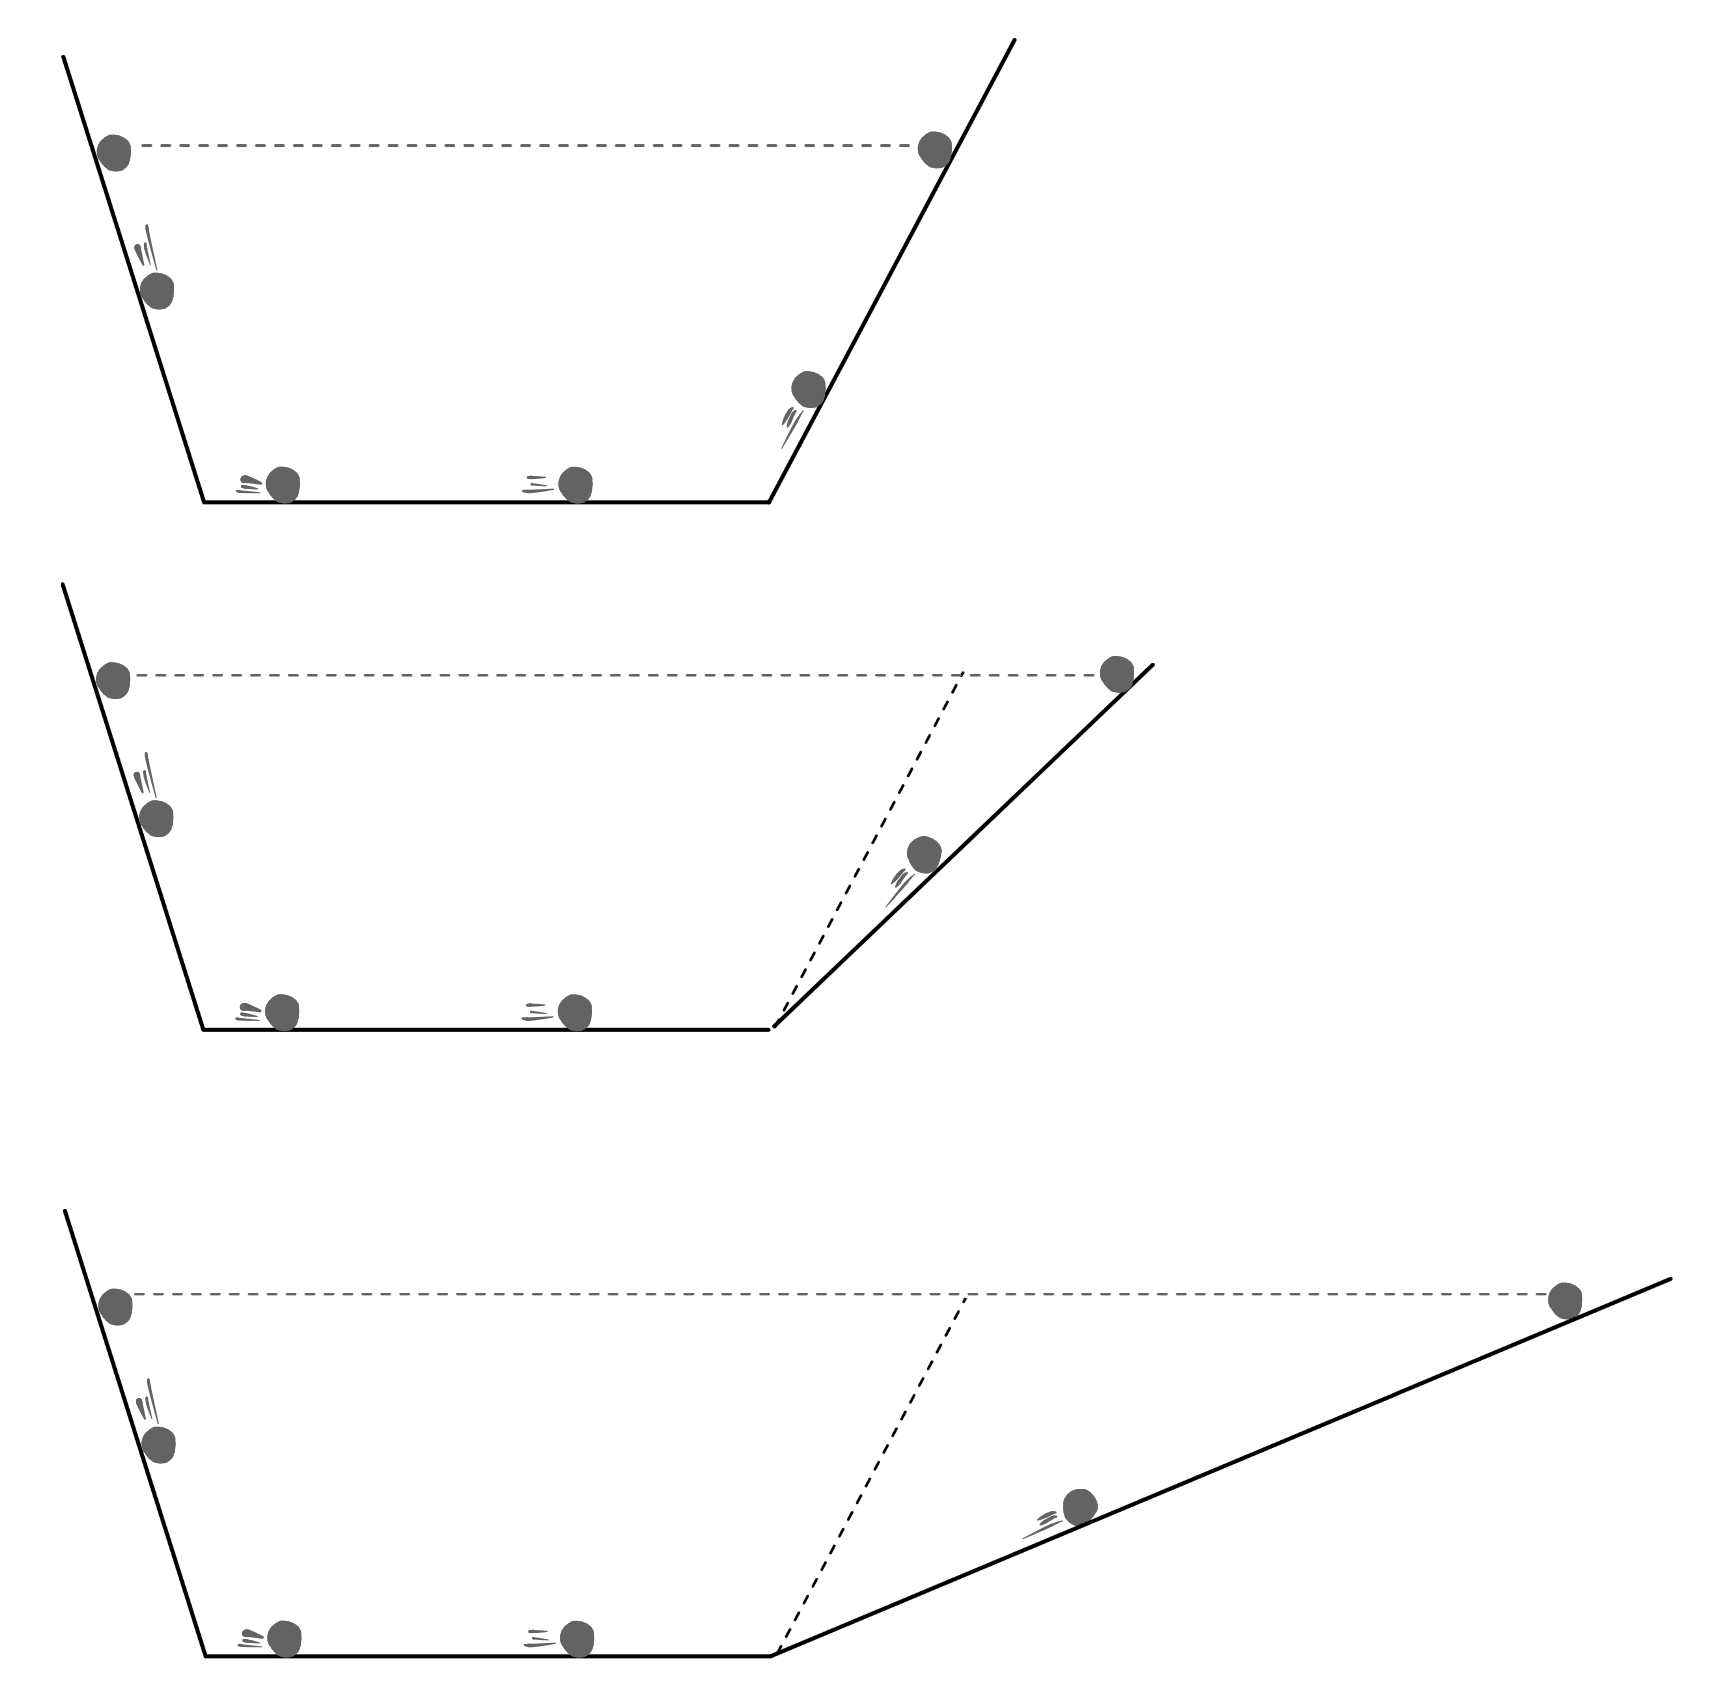
\includegraphics[width=0.6\linewidth]{imagensdinamicanewton/f=ma4.png}};
  \end{scope}
\end{tikzpicture}
\captionof{figure}{Independente da inclinação da rampa a bolinha sempre alcança, do outro lado, a mesma altura.}
\label{fig_dinamicanewton_f=maplanoinclinado01}
} 
\vspace{0.3cm}

Mesmo descendo a inclinação do plano -- o que obrigaria a bolinha a percorrer cada vez mais distância na subida para alcançar a mesma altura -- este era o resultado: a bolinha sempre chegava do outro lado na mesma altura. Partindo da premissa de que essa sempre seria a forma com que a bolinha se comportaria, \footnote{Um estudante mais sabido diria que isso é uma consequência da lei da conservação da energia: a energia potencial $E=mgh$, na descida, se converte em energia cinética, que por sua vez se converte em energia potencial gravitacional de novo na subida da bolinha. Se não existe atrito, o sistema é conservativo e, portanto, a bolinha deve alcançar a mesma altura. Ok, isso faz sentido, mas seria anacrônico usar este raciocínio: na época de Galileu os conceitos de energia cinética, potencial ou de conservação da energia eram inexistentes. Portanto, por mais que ele não soubesse justificar o motivo, era isso que ele observava: as bolinhas sempre chegavam do outro lado na mesma altura. É como se a natureza tivesse uma lei, digamos, ``lei das alturas'', que obrigasse a bolinha a sempre chegar exatamente do outro lado na mesma altura. Galileu estava percebendo como a natureza funcionava, não por que ela funcionava daquela forma -- teorias futuras, como a da conservação da energia, se serviram para dar essa explicação, mas este não é o nosso foco ou interesse neste momento.}, Galileu indaga: \textit{o que aconteceria se deitássemos completamente o plano e reduzíssemos sua inclinação a zero?}

A Figura \ref{fig_dinamicanewton_f=maplanoinclinado02} ilustra a conclusão que o gênio tirou dessa pergunta: como a distância percorrida para chegar à mesma altura aumenta cada vez que deitamos o plano, no caso em que o deitarmos completamente, a distância que a bolinha teria que percorrer seria infinita: ela permaneceria se movendo, com a mesma velocidade, até o infinito. \footnote{Caso o leitor já tenha escutado que retas paralelas se encontram no infinito, perceba, pela imagem da Figura \ref{fig_dinamicanewton_f=maplanoinclinado02}, que, para que a bolinha retorne à mesma altura, a linha cheia, que representa o plano horizontal, teria que encontrar a linha pontilhada, que representa o mesmo nível de altura em que a bolinha foi abandonada. Assim, sendo essas linhas paralelas, a bolinha teria que ir até o infinito para chegar à mesma altura. Não espere que o leitor acredite que o autor tenha ido pessoalmente ao infinito para observar o suposto encontro das paralelas. Tal expedição, além de custosa, parece logisticamente complexa. Recebeu tal informação de um amigo -- sujeito de boa índole e de caráter sólido -- mas, como se vê, trata-se de um testemunho indireto. Quanto à comprovação empírica, resta-lhe a humildade de admitir que não a possui.} Tal movimento se daria sem a necessidade de ter qualquer força para manter a bolinha em movimento: o movimento se perpetuaria, de modo natural, na ausência de forças. Trata-se de um movimento bem especial, como a Figura \ref{fig_dinamicanewton_f=maplanoinclinado02} ilustra: o Movimento Uniforme em Linha Reta, como descrito por Isaac Newton, ou o Movimento Retilíneo Uniforme (MRU), como descrito atualmente nos almanaques de ensino de Física. É um movimento, em linha reta, com velocidade constante. 

Perceba que isso contraria a visão aristotélica de movimento: estamos falando de um movimento que se perpetua na ausência de forças, ou seja, \textbf{não é preciso nenhuma força para manter a bolinha neste movimento, o MRU.} A isso, futuramente, Isaac Newton deu o nome de inércia: a capacidade que um corpo tem de permanecer no seu estado de movimento. Ou seja, podemos dizer que a bolinha \textit{se move por inércia}: ela não precisa de nenhuma força para se manter em movimento; ela se move porque é assim que a natureza funciona -- corpos em movimento tendem a permanecer no seu estado de movimento, não é necessária força para mantê-los em movimento. A força é necessária apenas para alterar o seu estado de movimento.

\vspace{0.3cm}
{
\centering
\begin{tikzpicture}
  \begin{scope}[blend mode=multiply]
    \node {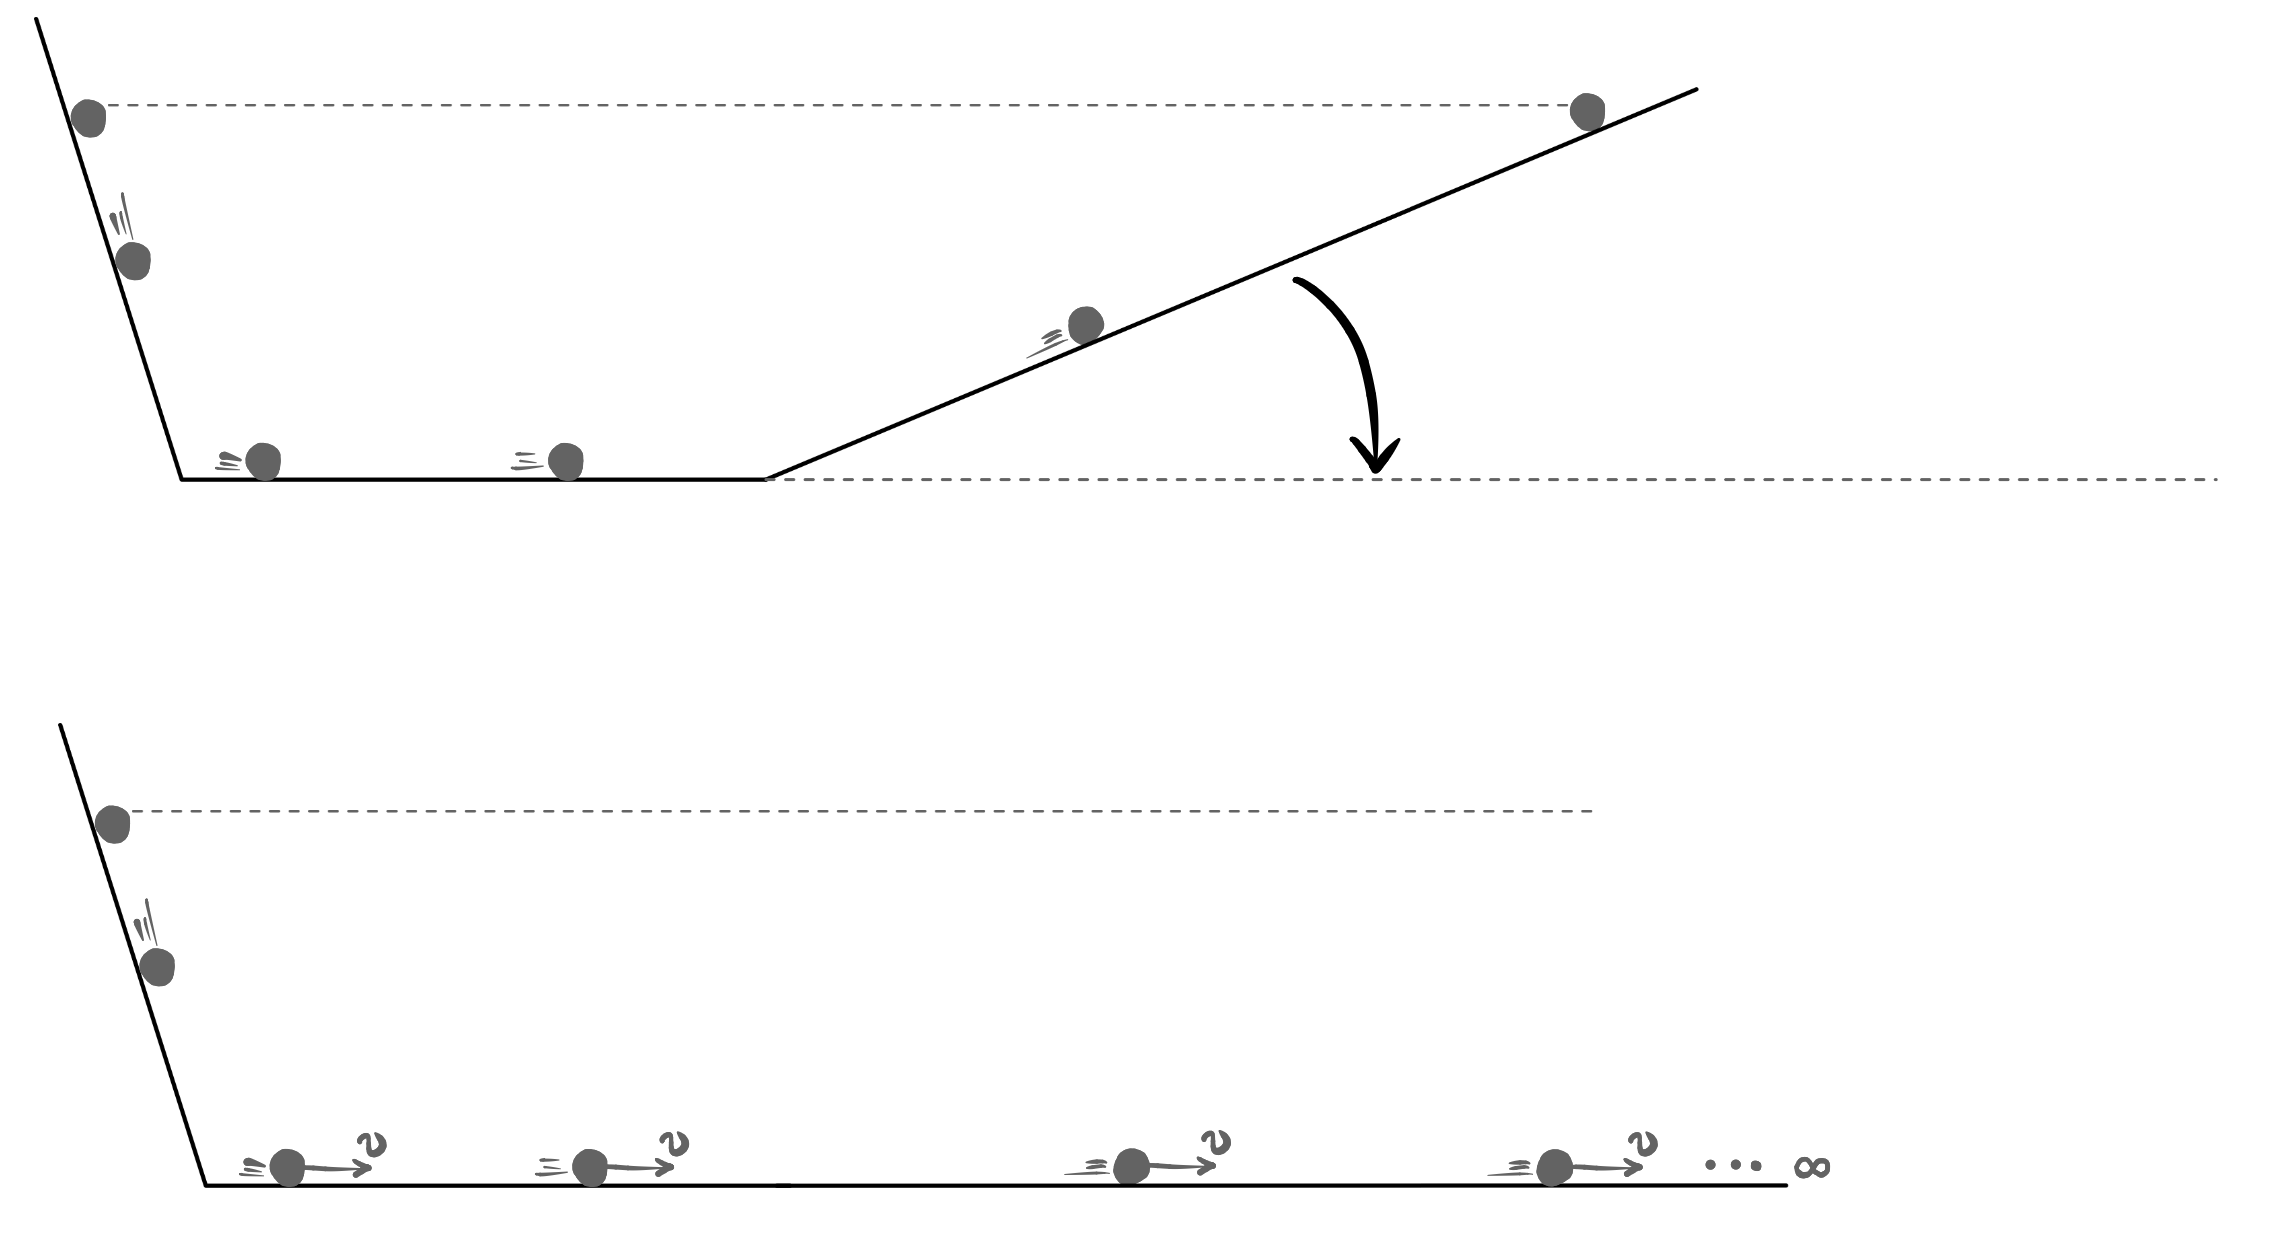
\includegraphics[width=0.8\linewidth]{imagensdinamicanewton/f=ma5.png}};
  \end{scope}
\end{tikzpicture}
\captionof{figure}{Ao reduzir a inclinação do plano a zero a bolinha teria que percorrer uma distância infinita para chegar à mesma altura.}
\label{fig_dinamicanewton_f=maplanoinclinado02}
} 

\vspace{0.3cm}



Os experimentos das três imagens da Figura \ref{fig_dinamicanewton_f=maplanoinclinado01} poderiam e foram, de fato, executados por Galileu. Já o experimento da segunda imagem da Figura \ref{fig_dinamicanewton_f=maplanoinclinado02} não foi executado por ele -- e sequer poderia sê-lo. Primeiro porque ele não tinha material infinito para produzir um plano de tamanho infinito. Mesmo que o tivesse, levaria um tempo infinito para observar a bolinha se movendo, bem, até o infinito. 

Logo, existe de fato um salto aqui -- um salto que, talvez, apenas um gênio conseguiria dar sozinho. O último experimento não foi realizado e, como visto, sequer poderia sê-lo. Foi uma conclusão tirada a respeito de como a coisa toda deveria funcionar em um caso que seria teórico, ideal e irrealizável na prática; partindo do entendimento tirado dos experimentos que eram de fato realizáveis. Galileu visualiza a estrutura com que a natureza parece funcionar, entende o que ela quer lhe comunicar e, finalmente, extrapola para o campo da abstração e tira a conclusão do caso que seria impossível de se realizar ou observar: na ausência perfeita de atrito, ao deitar completamente o plano, a bolinha teria que se mover indefinidamente, com a mesma velocidade, até o infinito. Logo, não se precisa de força alguma para mantê-la em movimento e, portanto, a força deixa de ser necessária para que haja movimento. Pronto: desconstruiu-se quase 2 mil anos de pensamento e uma nova ideia sobre o movimento começa a surgir.

A força, agora, é entendida como necessária para \textbf{alterar o movimento}:  se a bolinha está parada, é necessária uma força para colocá-la em movimento. Se ela está em movimento, é necessária alguma força para fazê-la andar mais depressa ou mais devagar -- mas não é preciso força para mantê-la em movimento:

$$ \boxed{\text{a força é necessária para que haja \textbf{variação} do movimento.} }$$

Se o leitor tentar realizar o experimento da Figura \ref{fig_dinamicanewton_f=maplanoinclinado02} vai perceber que a bolinha, diferente do que dissemos, não se move até o infinito. Ela, na verdade, se moverá por alguns metros ao longo do plano horizontal e irá parar logo depois. Isso ocorre porque é impossível ter uma superfície perfeitamente polida: por mais que se lixe ou lubrifique o material para tentar deixá-lo o mais liso possível, a fim de eliminar o atrito, isso nunca pode ser feito de forma perfeita, de modo que o atrito estará sempre presente, por menor que ele seja. 

Assim, sendo a força de atrito, neste caso, uma força que se opõe ao movimento e, como a força causa a variação do movimento, ela irá variar o movimento, diminuindo-o até ele cessar. Ou seja, a força aqui retarda a bolinha, fazendo-a parar -- e é por isso que, no experimento real, ela não vai até o infinito. Mais uma vez, é necessária a capacidade de pensar de forma abstrata para concluir o que Galileu conclui: é uma experiência de pensamento, feita na nossa cabeça, em um mundo ideal, e nos serve para entender, na sua essência mais pura, como o movimento funciona.

Perceba que a diferença entre a perspectiva Galileana/Newtoniana \footnote{Aqui não nos atemos a explicar muito essa diferença entre Galileu e Newton, mas ocorre que Galileu foi o primeiro a perceber essas ideias, mas não conseguiu unificá-las e estruturá-las em uma nova teoria completa a respeito do movimento, capaz de substituir a teoria aristotélica. Isso foi feito posteriormente por Isaac Newton.} em relação à Aristotélica é sutil: a visão aristotélica do movimento entendia que a força $F$ era necessária para que houvesse movimento, ou seja, sendo a velocidade $v$ a grandeza física que mede o movimento, teríamos que

$$ F \propto v,$$

\noindent ou seja, a força seria proporcional à velocidade, pensando em termos mais matemáticos. Já na visão Galileana/Newtoniana a força $F$ era necessária para que houvesse \textbf{variação} do movimento, ou seja, sendo a aceleração $a$ a grandeza física que mede o a variação do movimento, isto é, a variação da velocidade, teríamos que

$$ F \propto a,$$

\noindent ou seja, a força seria proporcional à aceleração, e não à velocidade.

Da relação de proporção direta acima para desaguarmos na Equação \eqref{eq_dinamica1_segundaleinewton} falta apenas um passo: adicionar a massa $m$ como constante de proporcionalidade e, voilà, temos a Segunda Lei de Newton: $F = ma.$ Em breve discutiremos a razão da massa ser a constante de proporcionalidade. Por ora, vamos nos atentar à sutil mudança de que agora a força é necessária para causar a variação do movimento, e não o movimento em si.


Note que, nessa nova perspectiva, o problema da Figura \ref{fig_dinamicanewton_f=ma1} não faria sentido: não tem como saber para onde o bloco se move só sabendo das forças, uma vez que agora a força não tem relação direta com o movimento, mas sim com a variação dele. Ainda no contexto de tal figura, em que $F_1 > F_2,$ isto é, a força resultante aponta para a direita, o bloco poderia ter diferentes velocidades, como ilustra a Figura \ref{fig_dinamicanewton_f=ma3}. O bloco poderia estar


\begin{enumerate}
    \item [(i)] se movendo para a direita -- ocasião em que o movimento seria acelerado, uma vez que a força resultante estaria a favor da velocidade, aumentando o movimento (aumentando a velocidade);
    \item [(ii)] se movendo para a esquerda -- ocasião na qual o movimento seria retardado, uma vez que a força resultante estaria no sentido contrário ao da velocidade, diminuindo o movimento (a velocidade);
    \item [(iii)] em repouso instantâneo, ou seja, $v=0$ -- ocasião na qual certamente o bloco começaria a se mover para a direita, uma vez que, sendo a força responsável por variar o movimento, estando ela para a direita, com o bloco em repouso, ela alteraria este estado de movimento (repouso) fazendo com que o bloco começasse a se mover na direção e sentido para a qual a força resultante aponta.
    
\end{enumerate}



{
\centering
\begin{tikzpicture}
  \begin{scope}[blend mode=multiply]
    \node {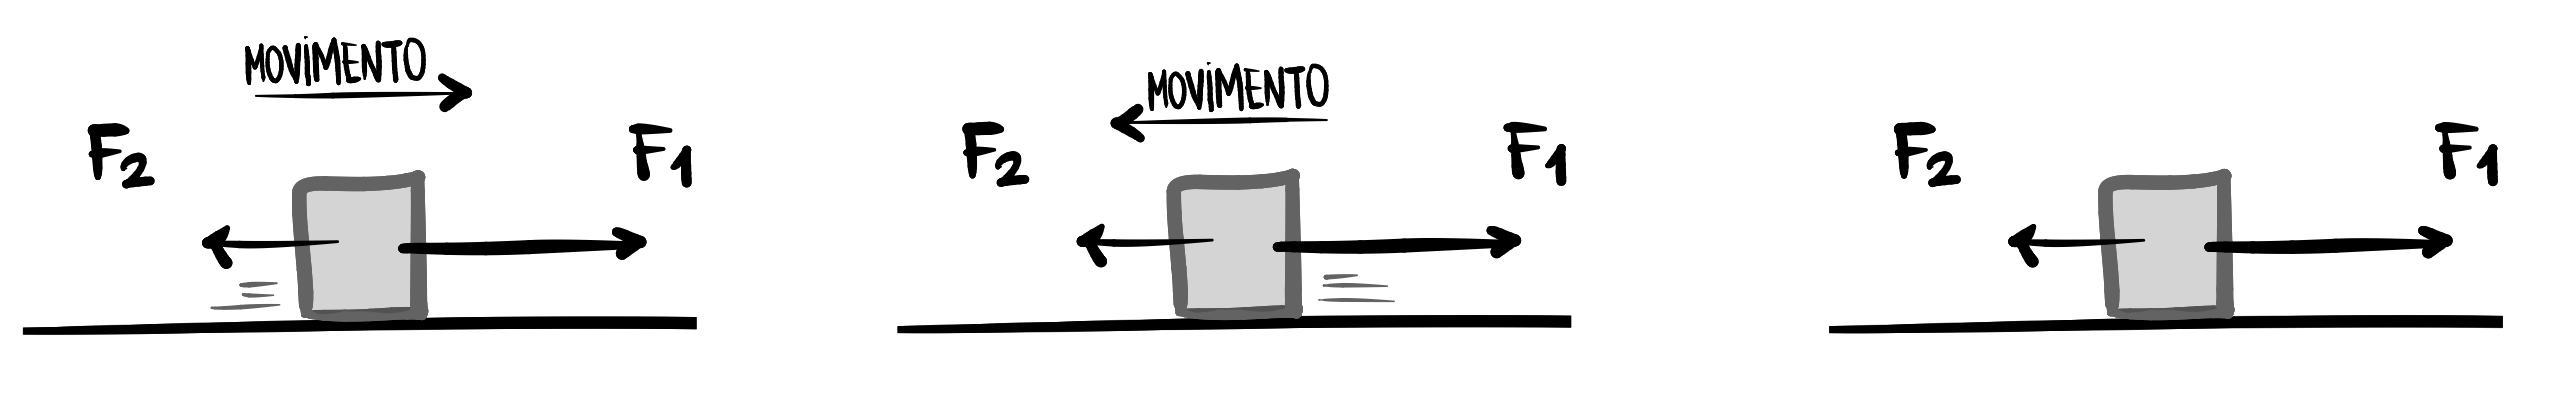
\includegraphics[width=0.8\linewidth]{imagensdinamicanewton/f=ma3.png}};
  \end{scope}
\end{tikzpicture}
\captionof{figure}{Tendo a força resultante para direita, o bloco pode ter qualquer tipo de velocidade, uma vez que a força não causa o movimento (velocidade) mas sim a sua variação (aceleração).}
\label{fig_dinamicanewton_f=ma3}
} 

\vspace{0.3cm}

Portanto, ao te fornecer a situação da Figura \ref{fig_dinamicanewton_f=ma1} e te perguntar para onde o bloco se move, tal pergunta deixa de fazer sentido no paradigma galileano/newtoniano, uma vez que, com forças, podemos determinar apenas como será a variação do movimento, e não o movimento em si. Como a \textbf{força causa a variação do movimento}, precisaríamos de, pelo menos, dois instantes distintos para tirar quaisquer conclusões, percebendo como o movimento varia de um instante para o outro.

\vspace{0.3cm}
{
\centering
\begin{tikzpicture}
  \begin{scope}[blend mode=multiply]
    \node {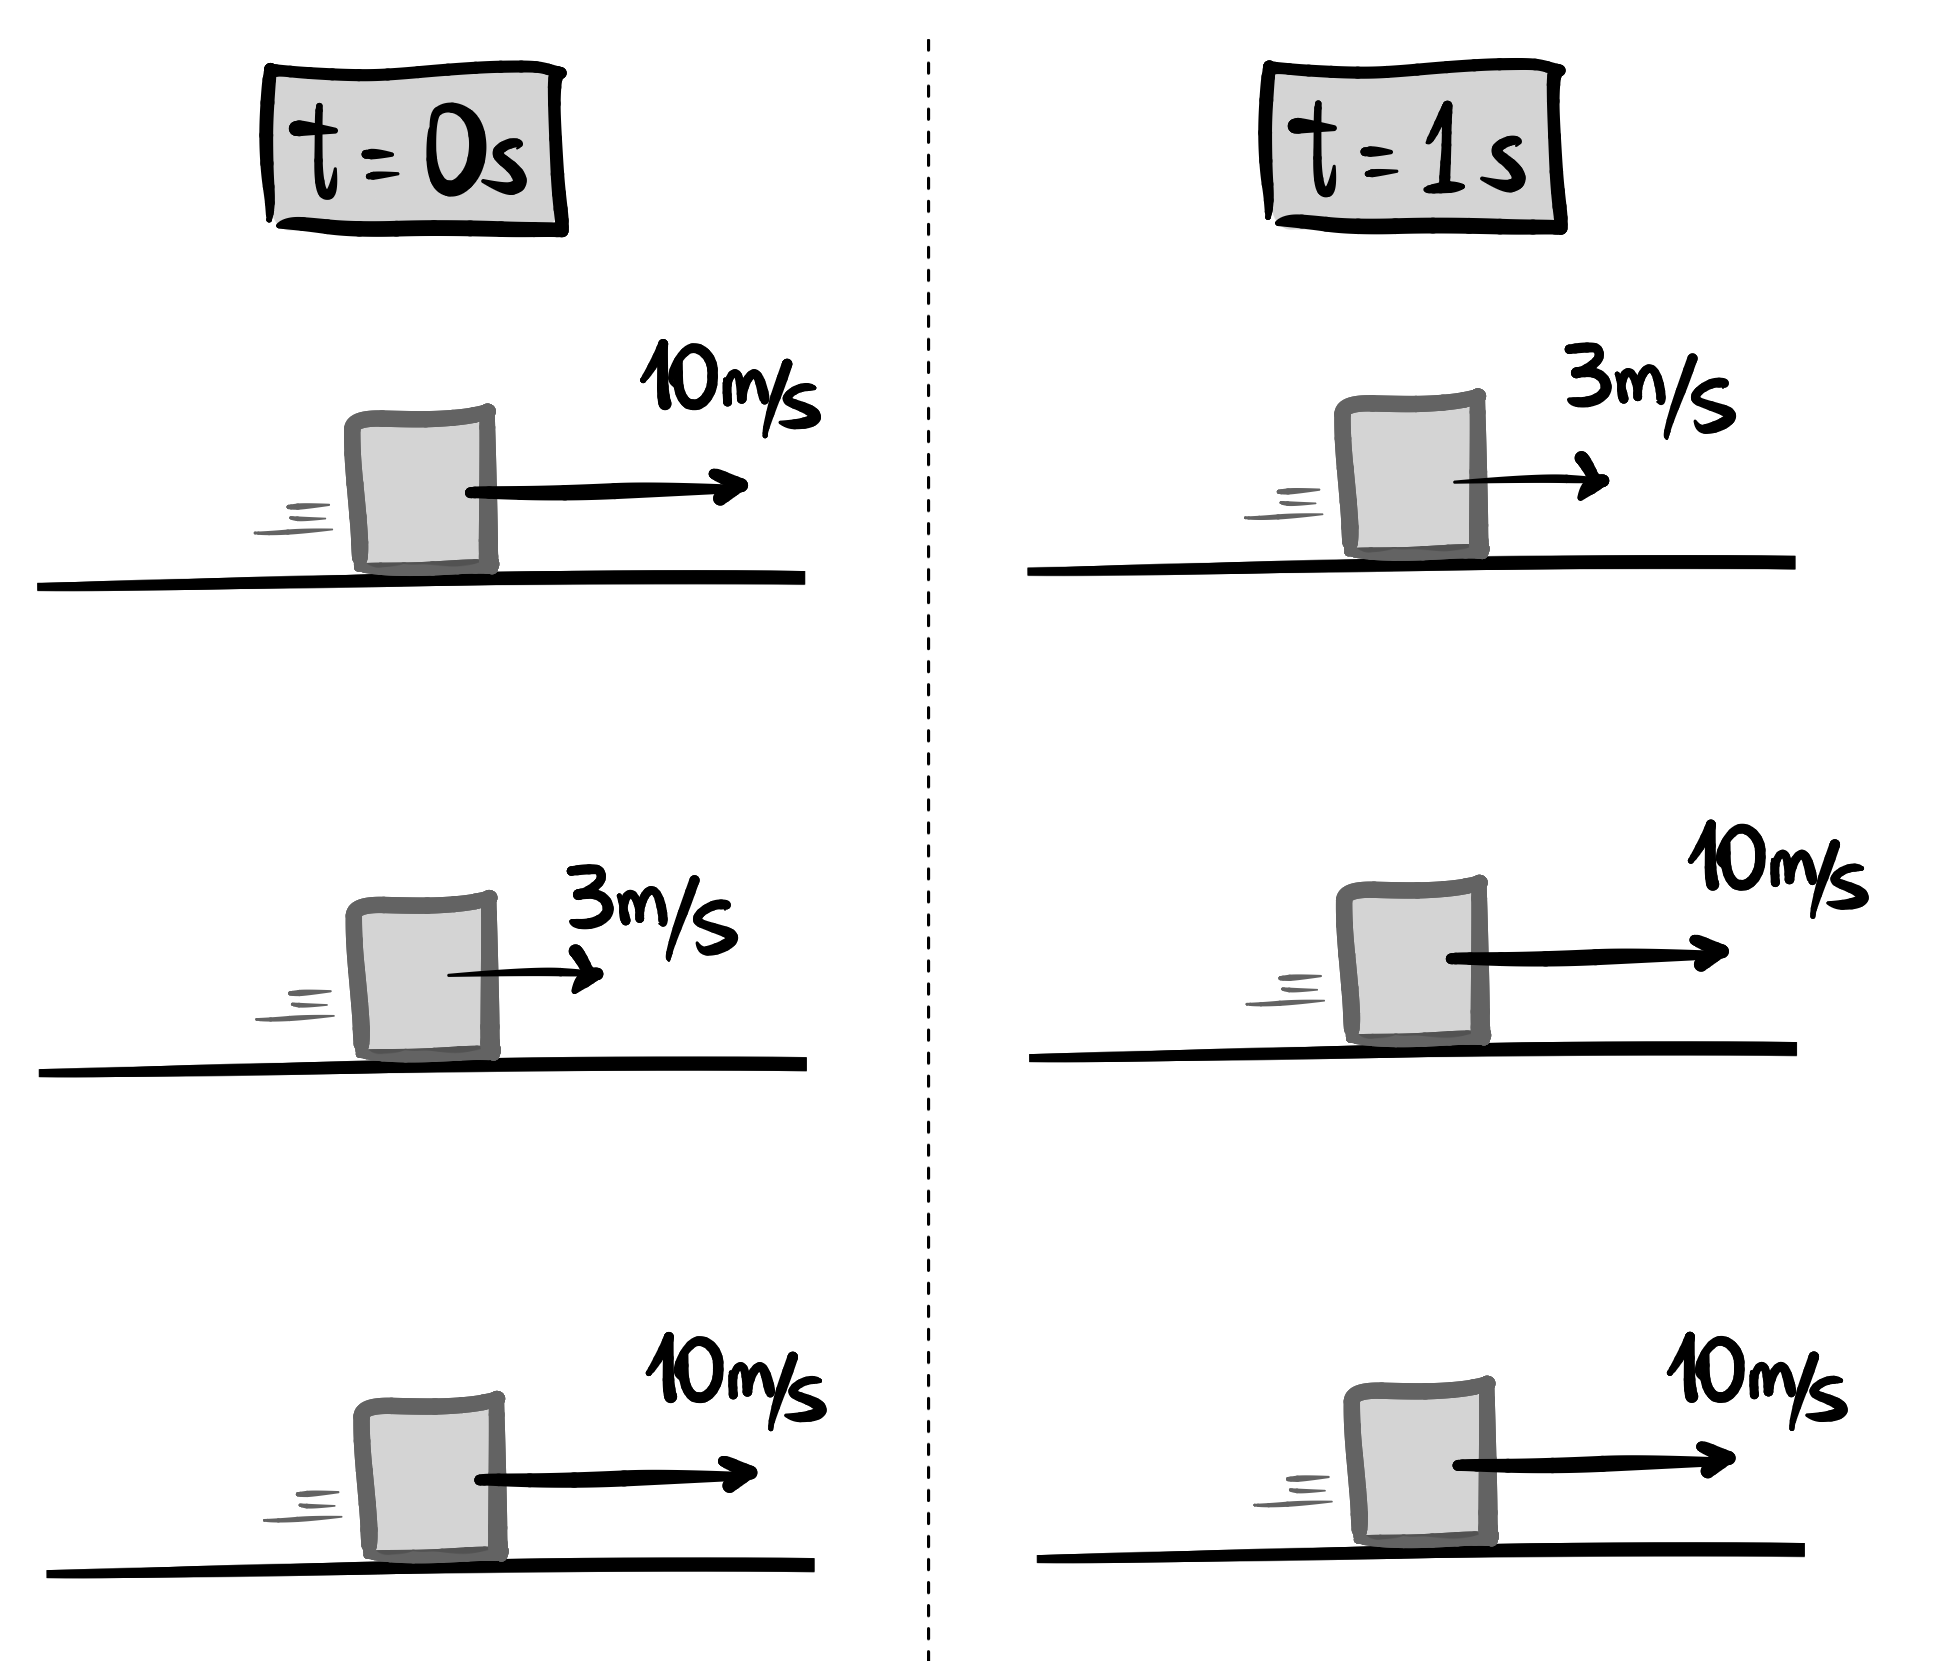
\includegraphics[width=0.4\linewidth]{imagensdinamicanewton/f=ma variacao movimento.png}};
  \end{scope}
\end{tikzpicture}
\captionof{figure}{Para obter informação sobre a força é preciso saber se houve variação do movimento (aceleração).}
\label{fig_dinamicanewton_f=ma variacao movimento}
} 
\vspace{0.3cm}

Essa é a situação da Figura \ref{fig_dinamicanewton_f=ma variacao movimento}, que mostra dois instantes distintos de um mesmo movimento. Ao avaliar o que ocorreu com o movimento (velocidade) de um instante para o outro, podemos concluir sobre a força que eventualmente atua no corpo. Avaliemos cada situação:

\begin{enumerate}
    \item [(i)] Na primeira linha, vemos que o movimento (velocidade) diminuiu de $t=0s$ para $t=1s$. Como houve variação do movimento, deve ter tido algum tipo de força para gerá-lo. Como o movimento (velocidade) diminuiu, concluímos que havia uma força contrária ao movimento, empurrando o bloco para a esquerda e gerando uma desaceleração nele.


    \item [(ii)] Na segunda linha, vemos que o movimento (velocidade) aumentou. Ora, se há variação do movimento, deve ter tido algum tipo de força para gerá-lo. Como o movimento (velocidade) aumentou, concluímos que havia uma força favorável ao movimento, empurrando o bloco para a direita e gerando uma aceleração nesse sentido.
     
    \item [(iii)] Na terceira linha percebemos que não houve variação no movimento de $t=0s$ para $t=1s$. Assim, concluímos que $F_R=0,$ isto é, se houver quaisquer tipos de forças atuando no bloco, elas devem se anular.\footnote{Vale destacar, correndo o risco de ser repetitivo: a condição $F_\text{R}=0$ não quer dizer que não há forças atuando no corpo. Podem sim haver forças, mas elas devem se anular.} Esse seria justamente o caso do MRU: o corpo tende a permanecer no seu estado de movimento, sem precisar de nenhum tipo de força para fazê-lo. A isso damos o nome de inércia.
\end{enumerate}


Acredito que já está mais do que clara a diferença entre a noção aristotélica e a noção galileana/newtoniana de movimento. Galileu foi o primeiro que começou a entender que não era preciso força para manter um corpo em movimento, mas foi Newton -- que nasceu em 1642, no mesmo ano em que Galileu morreu -- quem sintetizou e estruturou tudo isso.\footnote{ Inclusive, esse foi um dos erros cometidos por Galileu: para ele, a ideia de inércia não era restrita ao movimento retilíneo; ele admitia que podia haver uma espécie de \emph{inércia circular} em certos contextos. A definição completa e correta de inércia só viria com Newton.} A essa altura, é importante que o leitor perceba como a Equação \eqref{eq_dinamica1_segundaleinewton} condensa tudo o que conversamos até aqui: as conclusões do experimento dos planos inclinados estão capturadas ali; a ruptura com a física aristotélica está ali; a possibilidade de movimento na ausência de forças está ali. O que antes ocupava páginas de argumentação e descrição experimental agora repousa elegantemente em poucos símbolos.

Este é o verdadeiro poder de uma equação matemática: não apenas representar, mas sintetizar. Ela é capaz de comprimir uma longa sequência de raciocínios, experimentos e mudanças conceituais em uma expressão compacta. A Equação \eqref{eq_dinamica1_segundaleinewton} não inaugura a discussão — ela a encerra. Não é o ponto de partida do pensamento, mas o seu ponto de chegada: é nela que toda essa nossa longa conversa se organiza, se depura e se transforma em forma matemática.

Para perceber como tal equação contém a informação de que é possível a existência de movimento na ausência de força -- a grande ruptura com o paradigma aristotélico -- basta avaliar o que ela nos diz na ausência de forças, isto é, quando $F_R=0$:

$$ \vec F_R = m \vec a \xrightarrow{ \text{ } F_R = 0 \text{ } } \cancelto{0}{  \vec F_R }= m \cancelto{0}{  \vec a }  \xrightarrow{\text{  }} \vec a  =  0 \xrightarrow{ \text{ como } \vec a = \sfrac{\Delta \vec v}{\Delta t} \text{ }} \vec v \text{ é constante},  $$

\noindent ora, mas se o vetor velocidade $\vec v$ é constante, só há duas opções:

\begin{enumerate}
    \item [(i)] $\vec v = 0$, isto é, a partícula está em repouso. Este caso é simples e já estava dentro da visão de mundo aristotélica: na ausência de forças, um corpo deve necessariamente ficar em repouso, haja vista que o movimento, para Aristóteles, só pode se manter por meio da aplicação de forças.

    \item[(ii)] $\vec v$ é constante e diferente de zero. Por ser um vetor, para que ele seja constante é preciso que
       \begin{enumerate}
           \item Sua direção e sentido seja constante. Logo, o movimento deve ser \textbf{retilíneo}, uma vez que fazer curvas implica em mudar a direção do vetor velocidade.

           \item Seu valor (módulo) deve ser constante: o corpo não pode se mover mais rápido nem mais devagar, mas sempre na mesma velocidade. Ou seja, o movimento deve ser \textbf{uniforme.}
       \end{enumerate}

       Esta é a grande novidade na perspectiva Newton/Galileu: na ausência de forças, além do repouso, existe também um outro estado de movimento possível: o MRU. Aqui fica claro porque ele é tão especial: ele é o único movimento em que o vetor velocidade é constante em todas as suas características: a velocidade não muda em direção nem sentido (daí a necessidade de ser retilíneo) nem em valor (por isso o movimento é uniforme).
\end{enumerate}

Assim, a própria Equação \eqref{eq_dinamica1_segundaleinewton} contêm os dois possíveis estados de movimentos inerciais, ou seja, estados de movimento que ocorrem na ausência de forças: repouso \footnote{Talvez o leitor possa achar isso estranho, mas é comum nos referirmos ao repouso como um estado de movimento.} e MRU.


Estando claro a origem, história e significado da Equação  \eqref{eq_dinamica1_segundaleinewton}, resta-nos entender por que a massa $m$ é a constante de proporcionalidade que aparece ali. Tentarei ser breve nesta justificativa, para não correr o risco de me alongar mais do que o necessário -- mas certas equações, sobretudo esta, não se deixam atravessar com pressa. Sendo talvez a mais importante de toda a Física escolar, ela merece, sem dúvida, algum gasto adicional de palavras e de calorias do pensamento.

Indo direto ao ponto, o motivo principal da massa $m$ aparecer na Equação \eqref{eq_dinamica1_segundaleinewton} é porque a \textbf{massa é uma medida da inércia}, isto é, da capacidade que um corpo tem de permanecer em seu estado de movimento. Considere, por exemplo, um caminhão, inicialmente parado. Ao tentar empurrá-lo, ou seja, exercer uma força $F$, a fim de alterar seu estado de movimento -- colocá-lo em movimento -- o leitor há de encontrar certa dificuldade nessa tarefa. Isso porque, tendo o caminhão uma grande massa $m,$ sua inércia é muito alta: é difícil alterar o seu estado de movimento.

O mesmo valeria caso o caminhão estivesse se movendo a uma certa velocidade constante: é preciso muita força para pará-lo: sua inércia (tendência de permanecer no seu atual estado de movimento) é elevada, o que exige uma força maior para alterar seu estado de movimento.

Já um corpo de pouca massa, como uma bola de futebol, pode ter seu estado de movimento facilmente alterado com a aplicação de uma pequena força. Estando ela parada, com o chute de uma criança, conseguimos romper seu repouso e colocá-la em movimento. Estando ela em movimento, basta, talvez, o corpo de uma outra criança para interceptá-la e colocá-la em repouso: a inércia (massa) da bola é baixa, é preciso pouca força para alterar seu estado de movimento.

\vspace{0.3cm}
{
\centering
\begin{tikzpicture}
  \begin{scope}[blend mode=multiply]
    \node {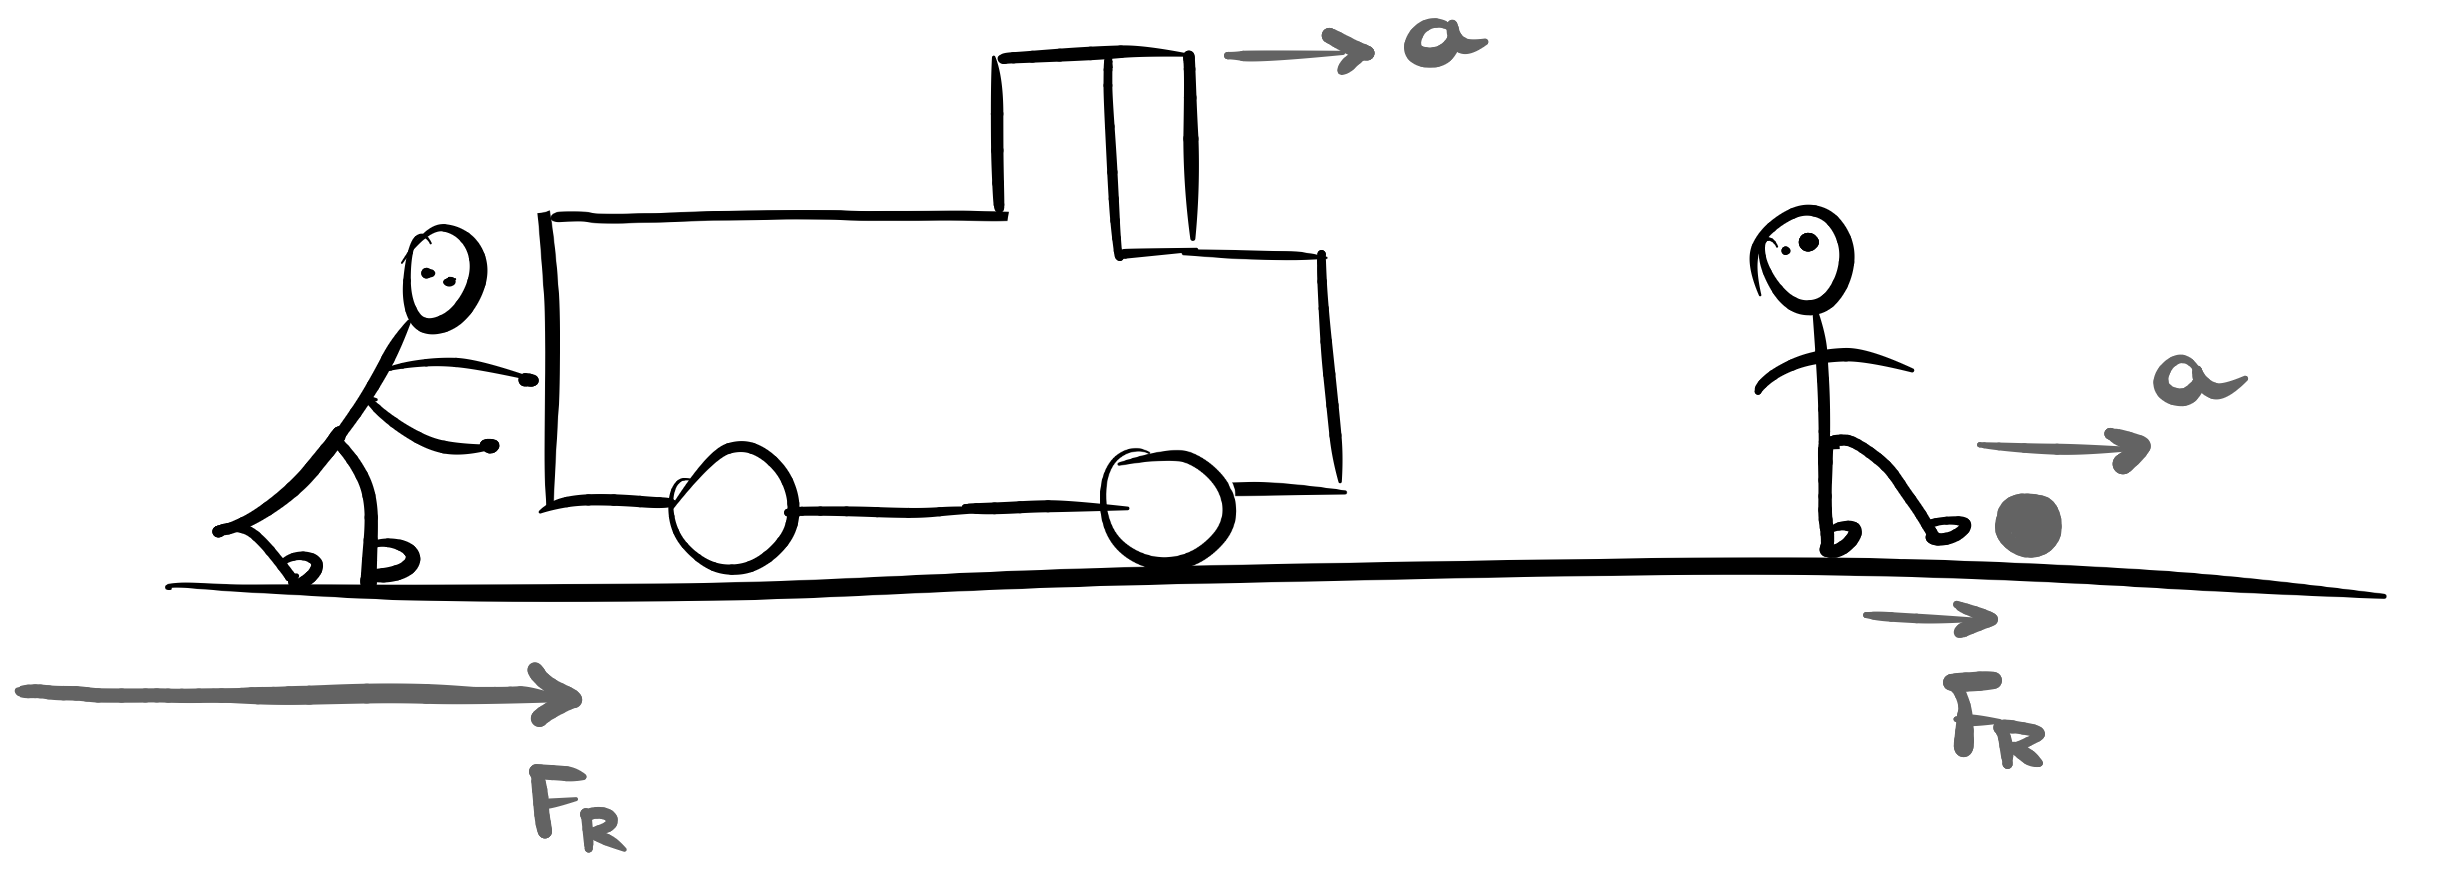
\includegraphics[width=0.6\linewidth]{imagensdinamicanewton/f=ma inercia massa.png}};
  \end{scope}
\end{tikzpicture}
\captionof{figure}{É preciso pouca força para alterar o estado de movimento de um corpo de pouca massa, mas muita força para alterar o estado de movimento de um corpo de muita massa.}
\label{fig_dinamicanewton_f=ma inercia massa}
} 

\vspace{0.3cm}

Com isso, conclui-se que a força resultante -- o agente que altera o estado de movimento de um corpo -- deve ser diretamente proporcional à massa do corpo cujo estado de movimento deseja-se alterar, uma vez que esta mede a capacidade de tal corpo permanecer em seu atual estado de movimento (inércia). É por isso que a massa $m$ é a constante de proporcionalidade que aparece na Segunda lei de Newton: corpos de maior massa (inércia) exigirão uma força maior (agente que causa a variação do movimento) para que se gere a mesma aceleração (variação do movimento). Podemos, inclusive, ler a Segunda Lei de Newton dessa forma:


$$  \underbrace{\text{(agente que causa a variação do movimento)}}_{\text{$F_R$}} = \underbrace{\text{(inércia)} }_{m} \cdot \underbrace{\text{(variação do movimento)}}_{a} .  $$




Logo, no caso do caminhão, como sua massa (inércia) é alta, é preciso mais força para gerar a mesma variação de movimento (aceleração):

$$  \underbrace{ \uparrow \text{(agente que causa a variação do movimento)}}_{\text{$F_R$}} = \underbrace{ \uparrow \text{(inércia)} }_{m} \cdot \underbrace{\text{(variação do movimento)}}_{a} .  $$



\secgfe{Onde é usada}



Essa é, com segurança, a equação mais importante de toda a Física estudada no Ensino Médio. Ela é o alicerce central de toda a mecânica newtoniana, que é a base de toda a Física que se desenvolveu nos 250 anos posteriores a Newton. 

Galileu morre em 1642, mesmo ano em que Newton nasce. Até o desenvolvimento da chamada Física Moderna – que se dá a partir de 1900, com o surgimento da Física Quântica por Planck e, posteriormente, com o desenvolvimento da Teoria da Relatividade Restrita de Einstein, em 1905 – praticamente tudo que é feito em Física neste longo intervalo de tempo é baseado na teoria mecânica de Newton e, consequentemente, na Equação \eqref{eq_dinamica1_segundaleinewton}.

Dito isso, as aplicações possíveis de tal equação dariam, por si só, um livro inteiro. Veremos, nas próximas seções, algumas equações que constituem certas aplicações. Mas que fique claro que o que veremos é apenas um copo d'água -- uma pequena porção do que contém o oceano. As aplicações são as mais diversas, como o estudo de corpos em movimento, o estudo de movimentos oscilatórios, de colisões de corpos, da trajetória e movimento de partículas que se movem sob a ação de um campo elétrico ou magnético, da interação eletrostática entre corpos carregados, etc. De modo geral, para estudar como se dá o movimento -- ou seja, qual é a aceleração -- de um corpo sob a ação de uma força qualquer -- seja ela uma força gravitacional, eletromagnética, elástica ou de qualquer outra natureza -- a Equação \eqref{eq_dinamica1_segundaleinewton} será a base inicial desse estudo: dada a expressão matemática da força, tal equação nos permitirá encontrar a aceleração deste corpo que é gerada pela aplicação de tal força, de tal sorte que, munidos da aceleração, poderemos fazer a descrição cinemática e compreender toda a evolução do movimento.


\secgfe{Erros comuns}

O erro mais comum é não compreender o caráter vetorial da Equação \eqref{eq_dinamica1_segundaleinewton}: trata-se de uma equação que envolve vetores, a força resultante $\vec{F}_R$ e a aceleração $\vec{a},$ respectivamente. Sendo assim, trabalhando com a decomposição vetorial, o mais comum é que façamos uma análise das forças em duas direções perpendiculares e, portanto, independentes.

\vspace{0.3cm}
{
\centering
\begin{tikzpicture}
  \begin{scope}[blend mode=multiply]
    \node {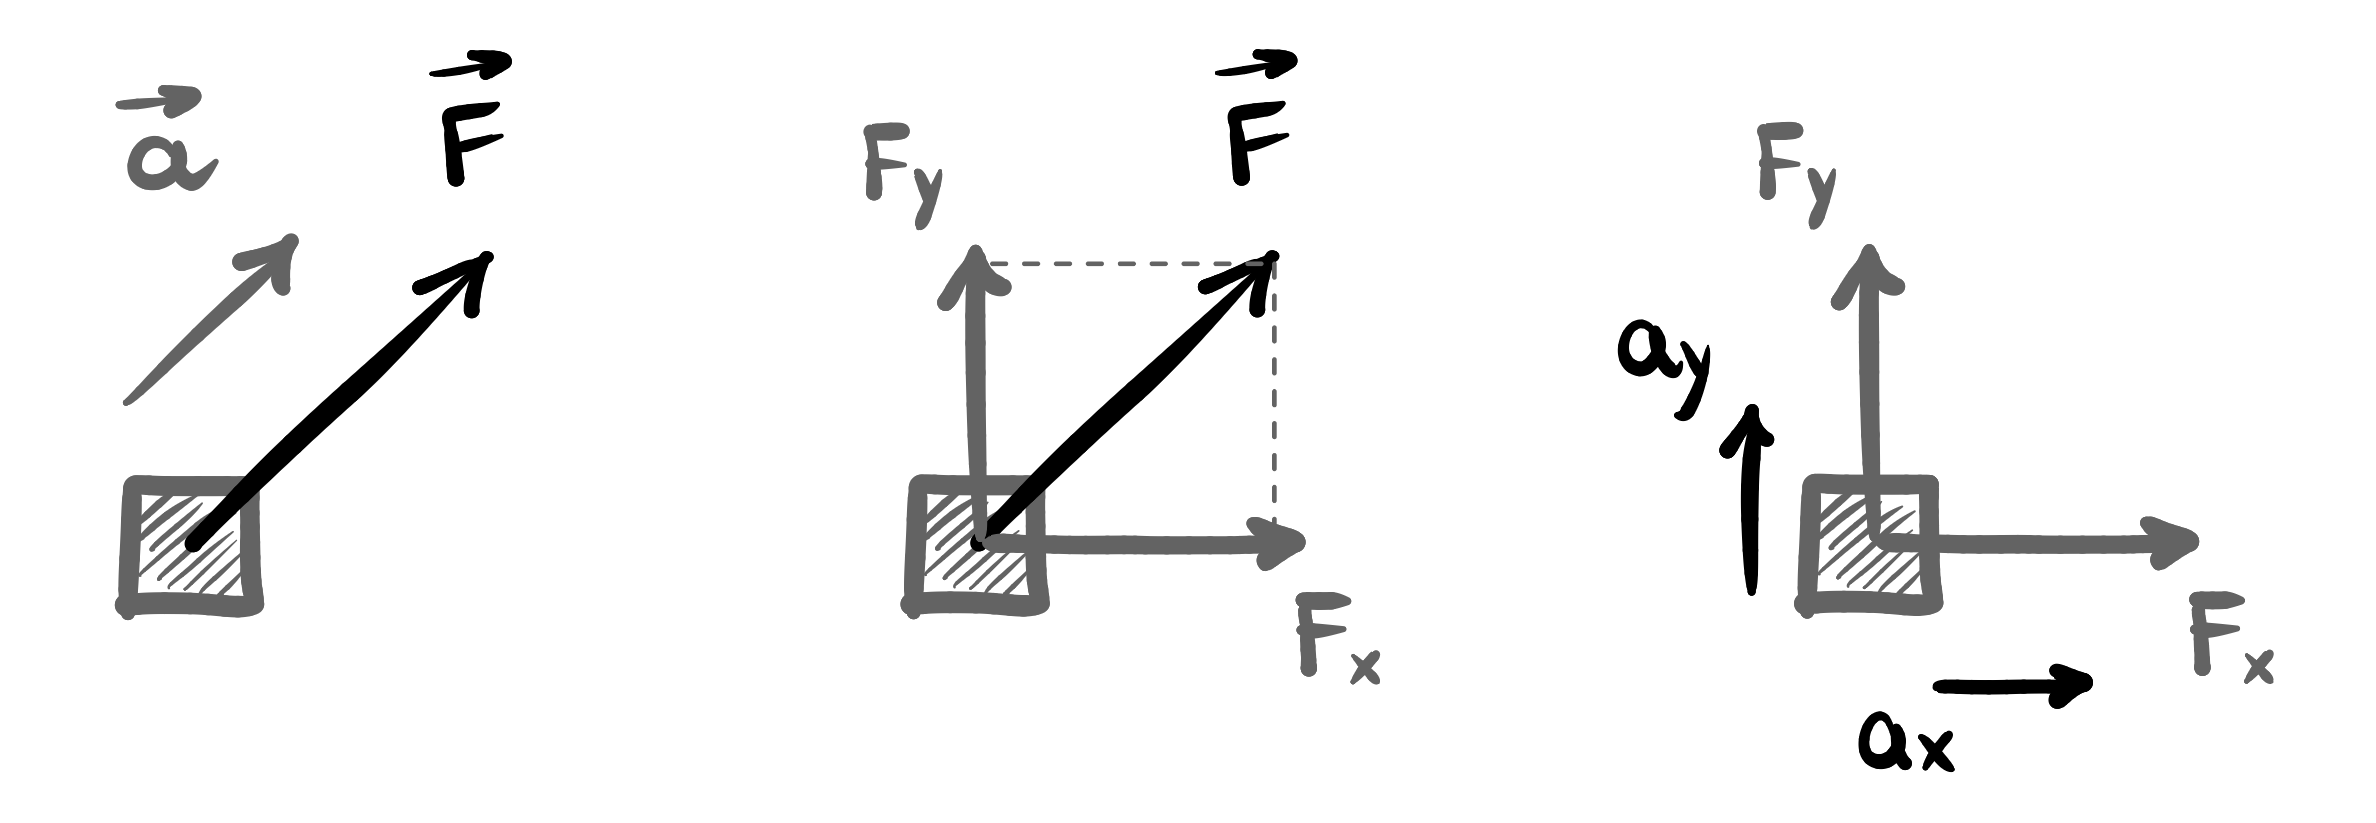
\includegraphics[width=0.6\linewidth]{imagensdinamicanewton/segundaleinewtondecomposicao2.png}};
  \end{scope}
\end{tikzpicture}
\captionof{figure}{A segunda lei de Newton aplicada em duas direções perpendiculares -- e, portanto, independentes.}
\label{fig_dinamicanewton_segundaleinewtondecomposicao2}
} 
\vspace{0.3cm}

Ou seja, como mostra a Figura \ref{fig_dinamicanewton_segundaleinewtondecomposicao2}, podemos compreender a força $\vec{F}$ como sendo a responsável por gerar a aceleração total $\vec a$ da partícula; ou, então, podemos decompor tal força em duas componentes nos eixos perpendiculares $x$ e $y$, originando as forças $\vec{F}_x$ e $\vec{F}_y$. Assim, tais forças gerariam as acelerações $\vec{a}_x$ e $\vec a_y,$ respectivamente. Este segundo caminho será o mais comum: analisarmos a resultante das forças em direções perpendiculares $x$ e $y,$ para compreender a aceleração gerada nessas duas direções.

Dito isso, sendo tal procedimento extremamente comum e corriqueiro na resolução de problemas sobre leis de Newton, os erros mais comuns cometidos pelos estudantes são dois:

\begin{enumerate}
    \item [(i)] Cometer erros na decomposição vetorial.

    Aqui podemos ter os mais variados tipos de erros: não compreender corretamente como funciona a decomposição vetorial, ou então, por lacunas no conhecimento matemático, não saber usar corretamente as razões trigonométricas seno e cosseno para calcular as componentes decompostas. Essa natureza de erros refere-se, majoritariamente, a falhas oriundas da matemática: o aluno não tem uma boa base em geometria/trigonometria e se confunde na decomposição dos vetores e nos cálculos geométricos necessários para fazê-lo.

    Como Galileu percebeu, \textit{``...o grande livro da Natureza está escrito em linguagem matemática, e seus caracteres são triângulos, círculos e outras figuras geométricas, sem os quais é humanamente impossível entender uma única palavra. Sem eles é uma errância, é um desatino vão num labirinto obscuro.''} 

    Sem matemática é impossível estudar Física -- certamente isso já está claro para o leitor ao longo da leitura de um guia de fórmulas matemáticas para o estudo de Física. Mas cabe ressaltar que, daqui em diante, os conhecimentos de matemática -- em particular os de geometria e trigonometria -- se farão mais presentes e relevantes do que nunca. A sua ausência ou insuficiência acaba se tornando o motivo de muitos erros e dificuldades dos estudantes nesse assunto.

    \item [(ii)] Fazer a escolha errada de eixos para a decomposição.


     Sendo necessário na quase totalidade dos problemas de dinâmica fazer a decomposição das forças nos dois eixos perpendiculares, fica a pergunta: \textit{quais eixos devem ser usados?}

 Já sabemos e acordamos que a decomposição de vetores será sempre feita em um par de eixos perpendiculares. Isso ocorre para que possamos usar o Teorema de Pitágoras, as razões trigonométricas no triângulo retângulo e o princípio de que movimentos em direções perpendiculares são independentes; logo, podemos aplicar de forma independente a Equação \eqref{eq_dinamica1_segundaleinewton} nas duas direções distintas $x$ e $y$:


\[
 \vec{F}_R = m\vec a
\quad \xrightarrow{\text{projeção nos eixos}}
\quad
\begin{cases}
F_x = m a_x \\
F_y = m a_y
\end{cases}
\]

Contudo, qual é a melhor escolha de eixos? Mesmo nos restringindo a eixos perpendiculares, existem uma infinidade deles. A Figura \ref{fig_dinamicanewton_segundaleinewtondecomposicao1}, que ilustra o movimento de um pêndulo, destaca três possíveis escolhas de pares de eixos $xy$ que podem ser utilizados para a decomposição das forças e análise da dinâmica do movimento.


\vspace{0.3cm}
{
\centering
\begin{tikzpicture}
  \begin{scope}[blend mode=multiply]
    \node {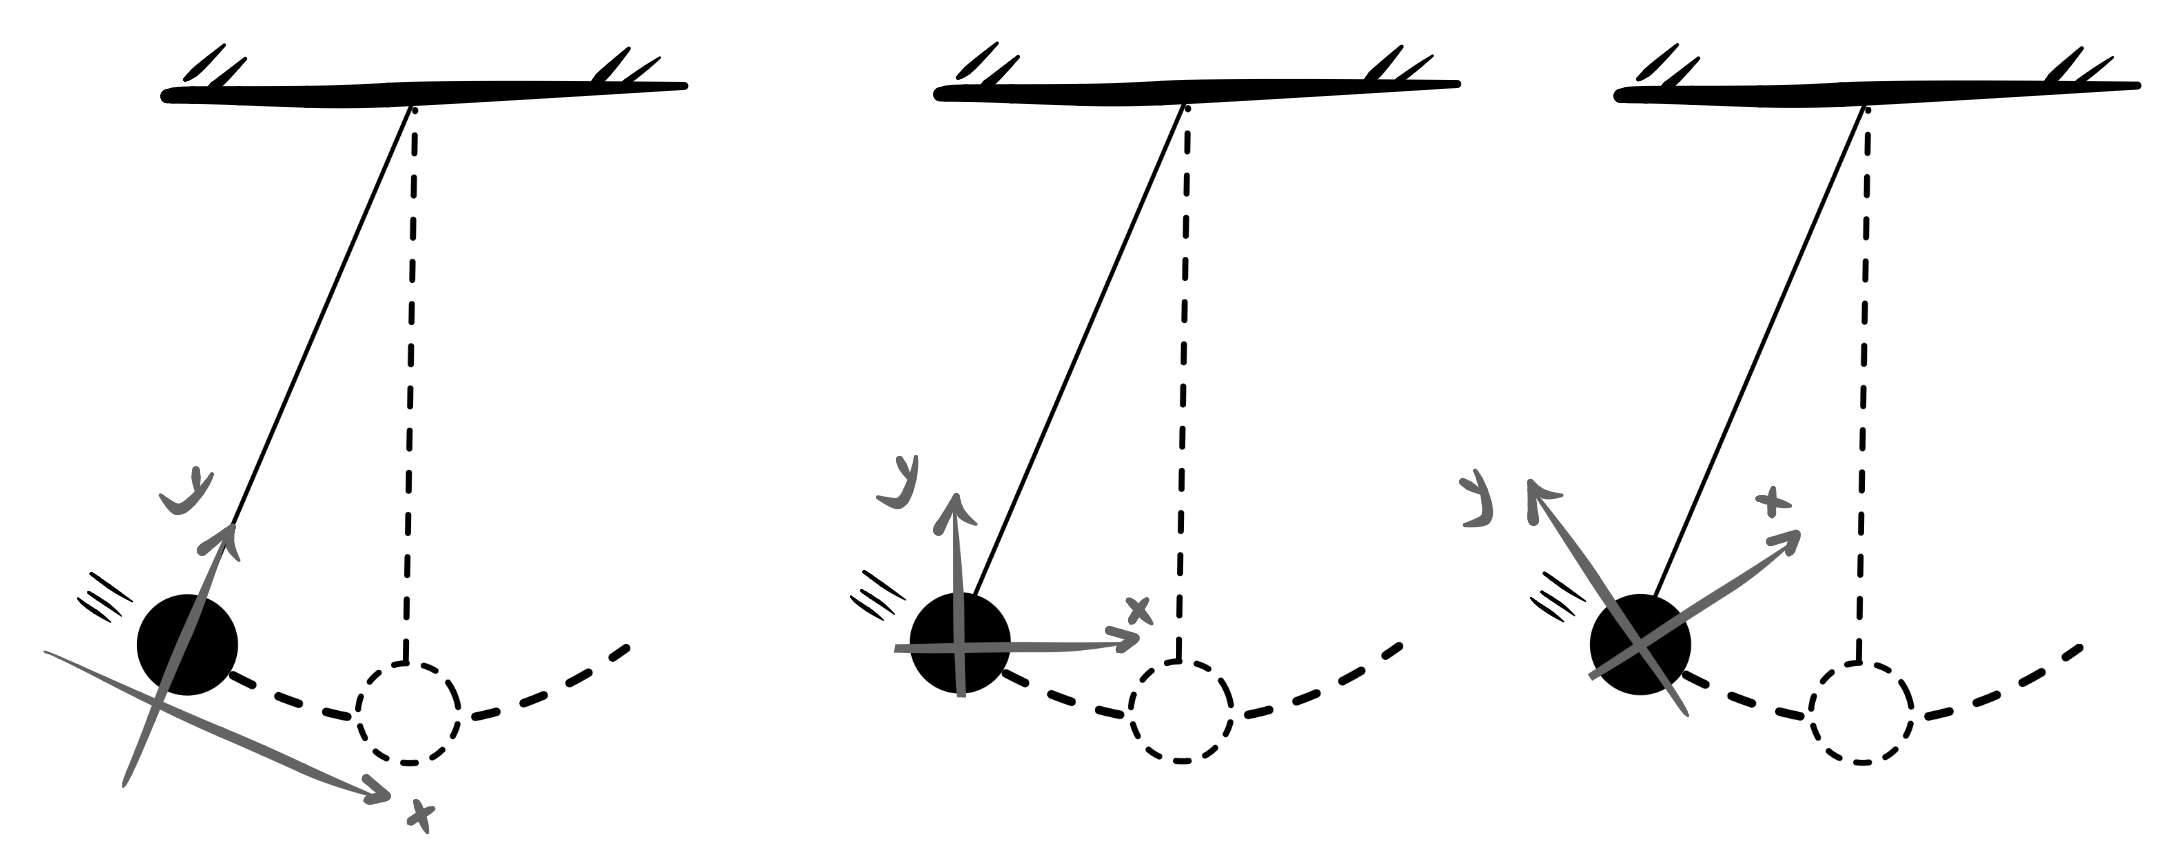
\includegraphics[width=0.6\linewidth]{imagensdinamicanewton/segundaleinewtondecomposicao1.png}};
  \end{scope}
\end{tikzpicture}
\captionof{figure}{Possíveis escolhas de eixos para fazer a decomposição vetorial das forças.}
\label{fig_dinamicanewton_segundaleinewtondecomposicao1}
} 
\vspace{0.3cm}


     Se o estudante não souber fazer essa escolha corretamente, a análise e o desenvolvimento matemático do problema se tornará (sem exageros) 5 vezes mais difícil, e acabará levando o leitor, com quase total certeza, a conclusões equivocadas e erros no meio do caminho. Esse é, possivelmente, o principal erro cometido em problemas que envolvam a Equação \eqref{eq_dinamica1_segundaleinewton}. 
     
     Para saciar a curiosidade dos mais ansiosos, a escolha mais adequada dos eixos de decomposição da situação da Figura \ref{fig_dinamicanewton_segundaleinewtondecomposicao1} é a da primeira imagem. Em breve entenderemos o porquê, e também faremos alguns exemplos para nos familiarizarmos com esse procedimento e conseguirmos sempre acertar nessa escolha de eixos, mas já adianto ao leitor qual será a regra de ouro para fazer a escolha correta:

 
        \textbf{A escolha dos eixos para fazer a decomposição vetorial e análise das forças que atuam em um corpo para que se aplique a Equação \eqref{eq_dinamica1_segundaleinewton} é tal que um dos eixos seja sempre paralelo ao vetor velocidade da partícula naquele ponto.}\footnote{A resultante das forças nesse eixo será responsável por gerar a aceleração tangencial (ou escalar) da partícula: aquela aceleração responsável por variar o módulo da sua velocidade.} 

         O segundo eixo já fica automaticamente definido pela exigência de ter de ser perpendicular ao primeiro.
   
    
\end{enumerate}




\secgfe{Observações}


A própria Equação \eqref{eq_dinamica1_segundaleinewton} já evidencia que a força é uma grandeza vetorial: ela precisa de módulo, direção e sentido para ser determinada. O vetor força sempre apontará na mesma direção e sentido do vetor aceleração, uma vez que o primeiro é o responsável por gerar o último. Logo, em um movimento retilíneo acelerado (aceleração e velocidade no mesmo sentido) a força terá o mesmo sentido da velocidade, enquanto que em um movimento retilíneo retardado (aceleração e velocidade em sentidos contrários) o vetor força terá sentido oposto ao do vetor velocidade.

A unidade de massa no Sistema Internacional de unidades de medida (SI) é o kg, enquanto que a unidade de aceleração no SI é m$\cdot$s$^{-2}.$ Assim, a unidade de força no SI é $\text{kg}\cdot\text{m}\cdot\text{s}^{-2}$, a que damos o nome de Newton (N):

$$ \boxed{\text{kg}\cdot\text{m}\cdot\text{s}^{-2} = N.}$$

Logo, se faz-se uma força em um objeto de $2$ kg de massa e gera-se nele uma aceleração de $5$ m/s$^2,$ tal força deve ser igual a
$$ F_R = ma \implies F_R = 2 \text{ kg} \cdot 5 \text{ m/s}^2 \implies F_R = 10 \text{ N.}$$

Como estamos introduzindo agora a Dinâmica, cabe fazer uma observação importante sobre a diferença entre ela e a Cinemática, que constituiu todo nosso estudo até então.  A Cinemática e a Dinâmica tratam do movimento, mas não fazem o mesmo tipo de pergunta. A Cinemática descreve, enquanto a Dinâmica explica.

Quando escrevemos
\[
s(t)=s_0+v_0 t+\frac12 at^2,
\]
estamos apenas descrevendo como a posição varia no tempo. A equação nada nos diz sobre \emph{por que} a aceleração tem determinado valor. Ela aceita a aceleração como um dado e constrói, a partir dela, o movimento.

A Segunda Lei de Newton muda completamente o cenário:

$$ \vec F_R = m\vec a.$$
 

Agora, a aceleração deixa de ser um dado arbitrário e passa a ser consequência de algo físico: a força resultante. Essa é a transição essencial: na Cinemática, a aceleração é um dado que aceitamos; já na Dinâmica, a aceleração é determinada por causas.


Em termos conceituais, a Segunda Lei introduz uma estrutura de causalidade, a de que a aceleração é causada pela força:
\[
\text{força resultante} \longrightarrow \text{aceleração}.
\]

A força não produz velocidade diretamente. Ela produz variação da velocidade.  Esse detalhe, aparentemente pequeno, é o que diferencia a mecânica newtoniana da aristotélica e é a base de toda a mecânica clássica, como vimos. 

É por isso que um corpo pode mover-se com velocidade constante mesmo sob ausência total de forças --- algo que a intuição pré-newtoniana não aceitava. O movimento uniforme não precisa de causa contínua; apenas a mudança do movimento exige isso.

% Essa estrutura causal é determinista: dadas as condições iniciais do movimento (onde a partícula estava inicialmente e qual era sua velocidade no instante inicial do movimento) e conhecidas as forças atuantes, o movimento está completamente determinado. Essa foi uma das grandes revoluções intelectuais da ciência moderna.


Desse modo, a Cinemática responde à pergunta ``como o corpo se move?'', enquanto a Dinâmica responde à pergunta ``por que ele se move assim?'' A primeira descreve trajetórias; a segunda constrói o mecanismo que as produz. 

\medskip

Uma outra observação bastante importante é o fato de que a Segunda Lei de Newton afirma que a força resultante determina a aceleração, mas ela não nos diz o que é a força. Ela não explica por que a Terra atrai a Lua; ou por que cargas elétricas interagem; ou por que dois corpos em contato exercem forças normais, etc. Ela apenas estabelece o que acontece quando uma força está presente.

Essa distinção é fundamental. Muitas vezes o estudante imagina que $ \vec F = m\vec a$ seja uma teoria completa do movimento. Não é. Ela é uma estrutura geral dentro da qual diferentes interações podem ser inseridas. 

A gravidade, a força elétrica e a força elástica, por exemplo, são descritas respectivamente por


$$ F_G = \,G\frac{Mm}{r^2}, \quad F_E = K\frac{q_1 q_2}{r^2} \quad \text{e} \quad  F = -k x  $$

\vspace{0.3cm}
{
\centering
\begin{tikzpicture}
  \begin{scope}[blend mode=multiply]
    \node {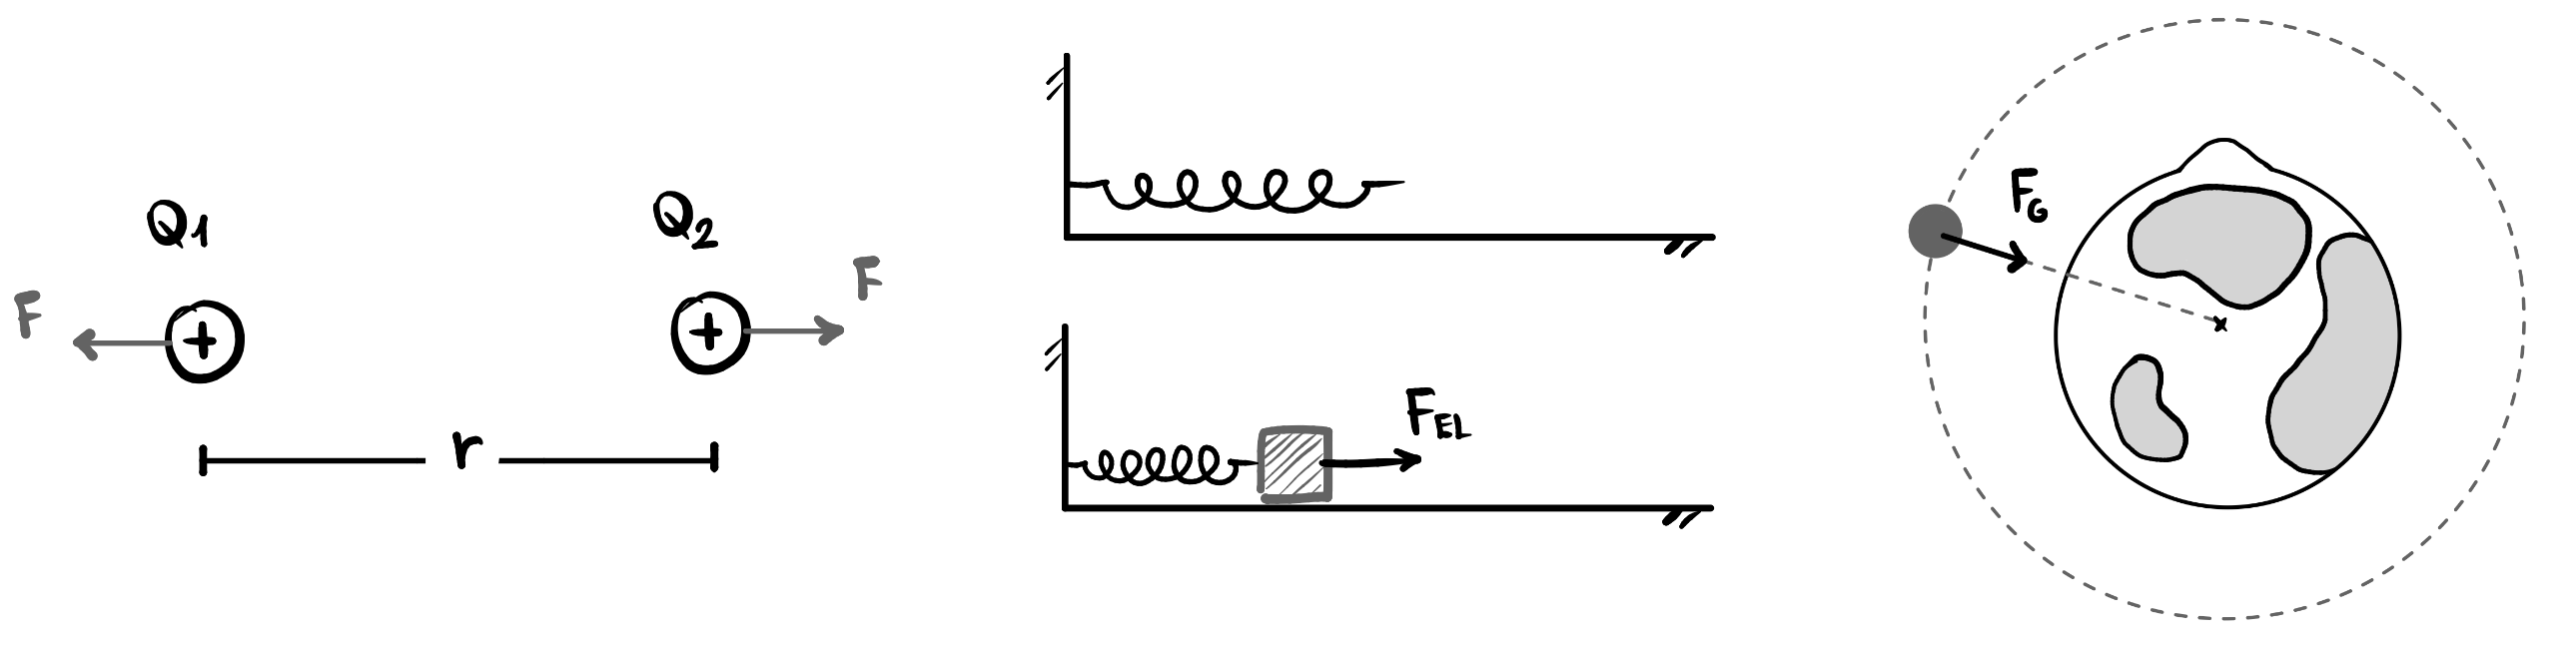
\includegraphics[width=1.0\linewidth]{imagensdinamicanewton/dinamicaforcasrepresentacaoexemplo.png}};
  \end{scope}
\end{tikzpicture}
\captionof{figure}{Representação das forças de interação elétrica, elástica e gravitacional.}
\label{fig_dinamicanewton_dinamicaforcasrepresentacaoexemplo}
} 
\vspace{0.3cm}

Essas três forças se encontram representadas, respectivamente, na Figura \ref{fig_dinamicanewton_dinamicaforcasrepresentacaoexemplo}: a força elétrica é a força de interação entre corpos carregados eletricamente (e é estudada em detalhes no volume III dessa coleção), a força elástica é a força que se manifesta em uma mola comprimida, e é estudada na Equação \eqref{eq_dinamicanewton_leihooke}; e, por fim, a força gravitacional é a força de interação entre corpos massivos -- a força de interação entre a Terra e a Lua, por exemplo -- e será estudada na Equação \eqref{eq_gravitacao_leigravitacaouniversal}.

Essas expressões não vêm da Segunda Lei. Elas são leis adicionais, obtidas por experimentos, e descrevem tipos específicos de interação. A Segunda Lei, portanto, atua como uma espécie de tradutor: como já vimos na Cinemática, a aceleração é a linguagem do movimento. Já as forças são a linguagem da interação -- sempre que corpos interagirem, tal interação será por meio de uma força (magnética, elétrica, elástica, gravitacional, etc). Assim, a segunda lei faz a tradução de como as forças -- a linguagem da interação entre corpos -- produzem aceleração, isto é, a linguagem do movimento. Desse modo, a Segunda Lei permite obter, por meio de como corpos interagem (forças), o elemento central (a aceleração) que a Cinemática precisa para fazer a descrição do movimento como um todo. O procedimento, portanto, sempre é:

\begin{enumerate}
\item  Escolhe-se o corpo cujo movimento desejamos estudar.
\item  Identificam-se as forças que nele atuam.
\item  Somam-se as forças vetorialmente.
\item  Com a Segunda Lei, determina-se a aceleração do corpo.
\item  Com a aceleração, a Cinemática já tem tudo o que precisa para descrever o movimento do corpo.
\end{enumerate}


O segundo exemplo que faremos na sequência ilustrará com clareza a execução desse procedimento.


É importante perceber que a natureza das forças pertence a outras teorias. Essa separação mostra a grandeza e vastidão da aplicabilidade da Equação \eqref{eq_dinamica1_segundaleinewton}: ela permite que a mecânica clássica seja um arcabouço geral, dentro do qual diferentes fenômenos podem ser descritos, desde que se conheça a estrutura das forças de cada fenômeno específico. E é por isso que tal equação é tão central no estudo da Física.



\vspace{0.3cm}

\begin{exemplo}[Nível I]\label{exemplo_dinamica1_eq_dinamica1_segundaleinewtonex01}

Uma partícula de massa $m=2$kg tem um movimento retilíneo e acelerado, sob a ação de apenas duas forças, como mostra a Figura \ref{fig_dinamicanewton_f=ma1} (p.~\pageref{fig_dinamicanewton_f=ma1}). Se o módulo da sua aceleração é $a=3$ m/s$^2$ e $F_1 = 50N,$ calcule o valor de $F_2.$



\resolucao

Pela segunda lei de Newton temos

$$ F_R = ma = 2 \text{ kg} \cdot 3 \text{m/s}^2 \implies \boxed{ F_R = 6 \text{N}.}$$

A $\vec F_R$ é, na verdade, um vetor: é a soma vetorial de todas as forças que atuam no corpo, computando a força resultante que nele atua, ou seja:

$$ \vec F_R = \vec F_1 + \vec F_2.$$

Já estudamos em detalhes a soma de vetores, que no caso da Figura \ref{fig_dinamicanewton_f=ma1}, em que eles apontam em direções contrárias, o módulo do vetor soma é dado pela diferença entre os módulos dos vetores somados, isto é:

$$ F_R = F_1 - F_2 \implies 6 = 50 - F_2 \implies \boxed{F_2 = 44 \text{N.}} $$



\end{exemplo}

\vspace{0.3cm}



\begin{exemplo}[Nível II]\label{exemplo_dinamica1_eq_dinamica1_segundaleinewtonex02}

Um bloco se move em linha reta em um plano horizontal. Sua velocidade inicial é $v_0=20$ m/s e ele enfrenta uma força de atrito constante de valor igual a $10$ N. Sendo a massa do bloco $m=2$ kg, encontre a distância total que ele percorre até ser totalmente desacelerado pelo atrito.

\resolucao

O problema se dividirá em duas etapas: a primeira é a aplicação da Dinâmica, que nos fornecerá o resultado para segunda etapa, a análise Cinemática:

\begin{enumerate}
    \item [(i)] Dinâmica.

    Usando a Segunda Lei de Newton -- sendo a força de atrito $F_{AT}$ a única força que atua na direção do movimento -- teremos, para essa direção:

    $$ F_{AT}  = F_R = ma \implies 10 = 2 a \implies \boxed{a = 5 \text{ m/s}^2.}  $$

    Logo, como a equação é vetorial, isto é:

    $$ \vec F_{R} = m \vec a,$$

    \noindent a aceleração apontará exatamente na mesma direção e sentido da força de atrito (que é a força resultante nessa situação), isto é, no sentido oposto ao do movimento (velocidade). Teremos, portanto, um movimento retardado, como era esperado. Sendo o valor de tal aceleração constante, concluímos que se trata de um MUV, e podemos usar nossos conhecimentos de Cinemática sobre tal movimento para dar sequência no raciocínio.

    \item [(ii)] Cinemática.

    Daqui em diante tudo se reduz a um problema já resolvido por nós algumas vezes. Temos um bloco com velocidade inicial $v_0=$ 20 m/s, sofrendo uma desaceleração constante de $5$ m/s$^2$, e queremos saber a distância que ele percorre até parar, isto é, até atingir $v=0.$ Por se tratar de um MUV, uma boa equação para computar isso sem necessidade de cálculos intermediários é a Equação de Torricelli:

    $$ \cancelto{0}{v^2} = v_0^2 -2a \Delta s \implies \Delta s = \dfrac{v_0^2}{2a} = \dfrac{20^2}{2 \cdot 5} \implies \boxed{\Delta s = 40 \text{ m} .}$$
\end{enumerate}

Perceba como estamos empilhando conhecimentos. O passo $(ii)$ foi um problema já resolvido por nós na Cinemática. Com a Dinâmica o que fizemos foi construir um arcabouço teórico que nos permite, dadas as influências físicas que um corpo sente (forças), encontrar a sua aceleração. Munidos da aceleração -- caso ela seja constante -- todo o problema se reduzirá aos problemas já estudados de MUV.\\

Desse modo, quase todo problema de Dinâmica vai envolver Cinemática: as leis de Newton serão o passo inicial para encontrar a aceleração e, com essa, o restante do problema seguirá pelos caminhos já conhecidos da Cinemática.


\end{exemplo}

% \vspace{0.3 cm}

% Essa é uma amostra grátis do livro de Guia de Fórmulas Explicadas, de autoria do professor Felipe Guisoli. A previsão é que ele seja lançado em agosto de 2026. Até lá, você pode estudar toda a Física do ensino médio com essa mesma abordagem -- didática, profunda e completa -- pelo curso completo de Física do Universo Narrado, o Lições de Física, ministrado pelo mesmo professor.

% O QR Code abaixo te direcionará para um grupo exclusivo em que você terá acesso a uma oferta especial no dia 02/março para se matricular no UN.

% {
% \centering
% 
\includegraphics[width=0.4\linewidth]{imagensintro/qr-code (6).png}
% \captionof{figure}{Entre no grupo VIP para receber em primeira mão a oferta especial para se tornar aluno do UN em 2026.}
% \label{figura_lancamentoforadacurva2026}
% } 

%\newpage

\vspace{0.3cm}


%  \begin{exemplo}[Nível III]\label{exemplo_dinamica1_eq_dinamica1_segundaleinewtonex03}

% Dois blocos, de massas $m_1 = \SI{3{,}0}{kg}$ e $m_2 = \SI{2{,}0}{kg}$,
% estão em contato e são empurrados juntos por uma força horizontal
% $F = \SI{20}{N}$ aplicada sobre $m_1$, numa superfície sem atrito.
% Determine:

% \begin{enumerate}
%   \item [a)] a aceleração do conjunto;
%   \item [b)] a intensidade da força de contato $F_c$ que $m_1$ exerce sobre
%   $m_2$.
% \end{enumerate}

%  \resolucao

% O conceito mais importante deste problema está em perceber que
% $\vec{F}_R = m\vec{a}$ pode ser aplicada a \emph{subsistemas} ---
% não apenas ao objeto isolado ou ao sistema completo. A escolha inteligente
% do sistema de análise é, aqui, o cerne da solução.

% \medskip 

% \noindent\textit{a)} Sistema completo ($m_1 + m_2$):

% Quando tratamos os dois blocos como um único sistema, a força de contato
% entre eles torna-se uma força \emph{interna} --- e forças internas não
% aparecem na resultante externa do sistema. A única força externa
% horizontal é $F$. Portanto:

% \[
%   F = (m_1 + m_2)\,a
%   \;\Longrightarrow\;
%   a = \frac{F}{m_1 + m_2} = \frac{20}{3{,}0 + 2{,}0} = \frac{20}{5{,}0}
%     = \SI{4{,}0}{m/s^2}.
% \]

% \noindent\textit{b)} Subsistema $m_2$ isolado:

% O bloco $m_2$ não sente a força $F$ diretamente --- ele só ``sabe'' que ela
% existe porque $m_1$ o empurra. A única força horizontal sobre
% $m_2$ é exatamente a força de contato $F_c$. Aplicando $F_R = m_2\,a$:

% \[
%   F_c = m_2\,a = 2{,}0 \cdot 4{,}0 = \SI{8{,}0}{N}.
% \]

% % \noindent Verificação pelo subsistema $m_1$: sobre $m_1$ atuam $F$
% % para a frente e $F_c$ para trás (reação de $m_2$ sobre $m_1$, pela
% % Terceira Lei --- que formalizaremos na seção seguinte):

% % \[
% %   F - F_c = m_1\,a \;\Longrightarrow\; 20 - 8{,}0 = 3{,}0 \cdot 4{,}0
% %   = 12 \;\checkmark
% % \]

% \noindent O resultado $F_c = \SI{8{,}0}{N}$ merece uma leitura
% qualitativa: a força de contato não é $F$, nem $F/2$. Ela é a fração
% da força total que ``coube'' a $m_2$ na distribuição proporcional às
% massas:

% \[
%   F_c = F \cdot \frac{m_2}{m_1 + m_2} = 20 \cdot \frac{2{,}0}{5{,}0}
%       = \SI{8{,}0}{N}.
% \]

% \noindent Essa proporcionalidade é uma das primeiras manifestações de
% algo que o leitor encontrará repetidamente: em sistemas acoplados sem
% atrito, cada parte recebe da força total exatamente a parcela
% proporcional à sua inércia.

%  \end{exemplo}


\begin{exemplo}[Nível III]\label{exemplo_dinamica1_eq_dinamica1_segundaleinewtonex03}

Um corpo de massa $m$ parte do repouso. Uma força resultante constante $F$ atua sobre
ele por um intervalo de tempo $T$, após o que é imediatamente invertida --- mantendo
módulo $F$, porém no sentido contrário --- e continua atuando indefinidamente. Determine
o tempo que o corpo leva para retornar à posição de partida após a inversão, e a
velocidade com que passa por ela.



\resolucao

Sendo as forças constantes, as acelerações geradas por elas -- dadas por $a = F/m$ -- também serão constantes, de modo que os movimentos serão uniformemente variados. Na primeira fase, o corpo acelera a partir do repouso por um tempo $T$, atingindo

$$ v_{\max} = \cancelto{0}{v_0} + aT = \frac{FT}{m}, \qquad d_1 = \cancelto{0}{v_0} \cdot t  + \frac{1}{2}aT^2 = \frac{FT^2}{2m}. $$

Esta é a maior velocidade do movimento. Tomando $t = 0$ no instante da inversão e a
origem na posição de partida, a posição na segunda fase é

$$ x(t) = d_1 + v_{\max}\,t - \frac{1}{2}a\,t^2. $$

O retorno à origem ocorre quando $x(t) = 0$. Substituindo e multiplicando por $2m/F$:

$$ t^2 - 2Tt - T^2 = 0, $$

\noindent cujas raízes são

$$ t = T\!\left(1 \pm \sqrt{2}\right). $$

Tomando a raiz positiva:

$$ \boxed{t_{\text{retorno}} = T\!\left(1 + \sqrt{2}\right).} $$

A velocidade ao retornar à origem é

$$v = v_\text{max} - at \implies  v = \frac{FT}{m} - \frac{F}{m}\cdot T\!\left(1+\sqrt{2}\right)
     = -\frac{FT\sqrt{2}}{m}, $$

\noindent cujo módulo é

$$ \boxed{|v| = \frac{FT\sqrt{2}}{m} = \sqrt{2}\cdot v_{\max}.} $$

O corpo retorna à posição de partida com velocidade $\sqrt{2} \approx 1{,}41$ vezes
maior do que a velocidade máxima atingida durante a ida. Curioso, não?




\end{exemplo}

\vspace{0.3cm}









\begin{secnivel}[Peso]{I}{Peso}
  
  \eqLdois{exp}{eq_dinamicanewton_peso=mg}{P = mg}

\end{secnivel}






\secgfe{De onde vem}

Estudaremos em mais detalhes a força de interação entre corpos massivos, chamada de força gravitacional,\footnote{Ao estudar em mais detalhes a Lei da Gravitação Universal vamos entender como a Equação \eqref{eq_dinamicanewton_peso=mg} da força peso é uma lei experimental particular da lei da Gravitação de Newton.} cuja lei é dada pela Equação \eqref{eq_gravitacao_leigravitacaouniversal}. 

A força peso é justamente a força de interação gravitacional que todos os corpos aqui na Terra sentem, devido à atração gravitacional realizada pela Terra. Ela é dirigida para o centro da Terra, o que, para fins práticos, significa ser dirigida para o chão: é a força que faz com que os corpos caiam.

Experimentos feitos por Galileu evidenciaram que corpos de diferentes pesos em queda livre -- isto é, sob a ação exclusiva da força peso -- caem juntos. Ou seja, mesmo tendo massas diferentes, os corpos caem com a mesma aceleração $g$, que, na superfície da terra, é de $g \approx 9.81 $m/s$^2$. Ou seja, sendo $P$ o valor da força peso, e usando a Equação \eqref{eq_dinamica1_segundaleinewton}, teríamos que, sob a ação exclusiva da força peso, isto é, $F_R =P,$ teríamos:

$$ F_R = P = ma,$$


\noindent e, sendo $g$ a aceleração com os corpos caem sob ação da força peso -- e ela é a mesma independente da massa, como observado pelos experimentos -- temos

$$ P = mg,$$

\noindent que é a equação que queríamos construir.


\secgfe{Onde é usada}

Em praticamente todos os problemas envolvendo as leis de Newton. Sendo a quase totalidade desses problemas no contexto do planeta Terra, uma força que estará sempre presente, naturalmente, será a força peso. 

A aplicação mais direta é a queda livre e o lançamento vertical. Quando
um corpo é abandonado ou arremessado na vertical, o peso é a única força
que atua (desprezando o ar), e a Segunda Lei fornece imediatamente
$a = P/m = g$. É daqui que vem a aceleração gravitacional: ela não é
uma constante que ``existe por si só'' --- ela é a razão entre o peso
e a massa do corpo, e o fato de ser a mesma para todos os corpos é uma
consequência da proporcionalidade $P \propto m$ que a própria fórmula
expressa. Galileu não sabia escrever $P = mg$; mas foi exatamente isso
que ele descobriu ao soltar objetos de alturas diferentes em Pisa.

No estudo do plano inclinado, que veremos na Equação \eqref{eq_dinamicanewtoniana_gsintheta}, o peso é
decomposto em duas componentes: uma paralela ao plano, responsável pela
aceleração do objeto ao longo da rampa, e outra perpendicular, que
equilibra a força normal exercida pelo plano. Toda essa análise vetorial começa com o vetor
$\vec{P} = m\vec{g}$. O mesmo ocorre nos sistemas de polias, nos quais as tensões no fio são
determinadas a partir do peso dos blocos envolvidos: a polia redistribui
forças, mas não cria nem destrói peso. 

A Equação \eqref{eq_dinamicanewton_peso=mg}, portanto, será uma das mais presentes em nosso estudo daqui em diante.


\secgfe{Erros comuns}

O erro mais comum não seria tanto da aplicação em si da Equação \eqref{eq_dinamicanewton_peso=mg}, mas sim de uma interpretação dela: a força peso é maior quanto mais massa o corpo tiver, o que pode levar muitos a intuir que a aceleração com que corpos mais massivos caem seja maior, pelo fato da força que os puxa para baixo ser maior. Contudo, como a massa aparece na equação da força peso e também na equação da Segunda Lei de Newton, este efeito acaba se cancelando, fazendo com que corpos de diferentes massas tenham sempre a mesma aceleração quando sob a ação exclusiva da força peso. Isso pode ser facilmente mostrado usando a força peso como força resultante na Segunda Lei de Newton:

\begin{align}
    F_R &= ma \nonumber \\
    P &= ma  \nonumber \\
    \cancel mg &= \cancel ma, \nonumber 
\end{align}

\noindent de onde conclui-se que 

$$  \boxed{  a = g,} $$

\noindent ou seja, independente da massa, todos os corpos, sob ação única e exclusiva da força peso, caem com a mesma aceleração da gravidade $g.$ É por isso que o movimento de queda livre -- queda sob a ação exclusiva da gravidade -- é um exemplo de MUV, isto é, um movimento com aceleração constante.

\secgfe{Observações}

É importante perceber a diferença entre a massa $m$ de um corpo, que é uma propriedade intrínseca do corpo e mede a quantidade de matéria que ele contêm; do seu peso $P,$ que é uma propriedade que depende da sua massa $m$, mas também do valor do campo gravitacional $g$ da região na qual o corpo está inserido.

Considere, por exemplo, um indivíduo de massa $70$ kg. Na terra, em que a gravidade é $g_T \approx 10$ m/s$^2$, seu peso é

$$ P = mg = 70 \cdot 10 = 700 \text{ N,}$$

\noindent enquanto na lua, onde a gravidade é $g_L \approx 1.6$ m/s$^2$, sua massa -- propriedade intrínseca do indivíduo -- continua sendo de 70 kg, mas seu peso passa a ser de

$$ P = mg = 70 \cdot 1.6 = 112 \text{ N.}$$

Isso não quer dizer que o indivíduo ``\textit{emagreceu}'' ao ir para a lua -- sua massa continua sendo a mesma: 70 kg. Lá, contudo, como a gravidade é menos intensa, a força que o puxa para baixo e o mantém preso no chão -- o seu peso -- é menos intensa. É comum, ao se \textit{pesar} em uma balança, ler o resultado e dizer que o seu peso é de 70 kg. Isso, contudo, estaria impreciso do ponto de vista físico: sua massa é de 70 kg, não o seu peso. A massa informada é um propriedade específica sua, enquanto que o seu peso é uma força que é proporcional à sua massa, mas também depende da região em que você está (por depender do valor da gravidade).


\vspace{0.3cm}

\begin{exemplo}[Nível I]\label{exemplo_dinamicanewton_p=mg01}

Um corpo de massa $m=3$ kg é lançado verticalmente para cima com velocidade de 12 m/s. Se ele enfrenta, ao longo de toda a sua subida, uma força de resistência do ar constante e igual a $6$ N, qual é a altura máxima que ele atinge?

\resolucao

Para problemas desse tipo sempre assumimos que a situação se passa na superfície da Terra, na qual a gravidade -- caso não seja informado nenhum valor -- pode ser sempre considerada igual a 10 m/s$^2$. Logo, o peso do corpo é $P=mg=3\cdot 10 = 30$ N.

Ora, o corpo sente duas forças, ambas para baixo: o peso e a força de resistência do ar. Logo, a sua força resultante é a somatória dessas duas, apontando para baixo:

$$ F_R = 30 +  6 = 36 \text{ N}.$$

Logo, pela segunda lei de Newton:

$$ F_R = ma \implies 36 = 3a \implies a = 12 \text{ m/s$^2$}.$$

Perceba que a desaceleração que o corpo sofrerá na sua subida é ligeiramente maior do que a da gravidade $g$, que seria de $10$ m/s$^2$. Isso porque, além do peso puxando o corpo para baixo, há também a força de resistência do ar se opondo ao seu movimento. Essas duas forças, somadas, resultam em uma força que se opõe ao movimento maior do que seria se houvesse apenas o peso, e é por isso que elas, juntas, resultam em um valor de aceleração maior do que o da gravidade.

Daqui em diante trata-se de um problema de Cinemática: sendo a aceleração constante, temos um MUV. Podemos, por exemplo, resolver usando a Equação de Torricelli, em que, na altura máxima, a velocidade será nula:

$$ \cancelto{0}{v^2} = v_0^2 - 2 a \Delta s \implies \Delta s = \dfrac{v_0^2}{2a} = \dfrac{12^2}{2\cdot 12} = \boxed{ 6 \text{ m.}} $$

\end{exemplo}


\vspace{0.3cm}

\begin{exemplo}[Nível II]\label{exemplo_dinamicanewton_p=mg02}


A Figura \ref{fig_mec_pendulodenewtonexemplo21} mostra um vagão acelerado com um pêndulo no seu interior que permanece em repouso em relação ao vagão, fazendo um ângulo $\theta$ com a vertical. Encontre a aceleração do vagão.

\vspace{0.3cm}
{
\centering
\begin{tikzpicture}
  \begin{scope}[blend mode=multiply]
    \node {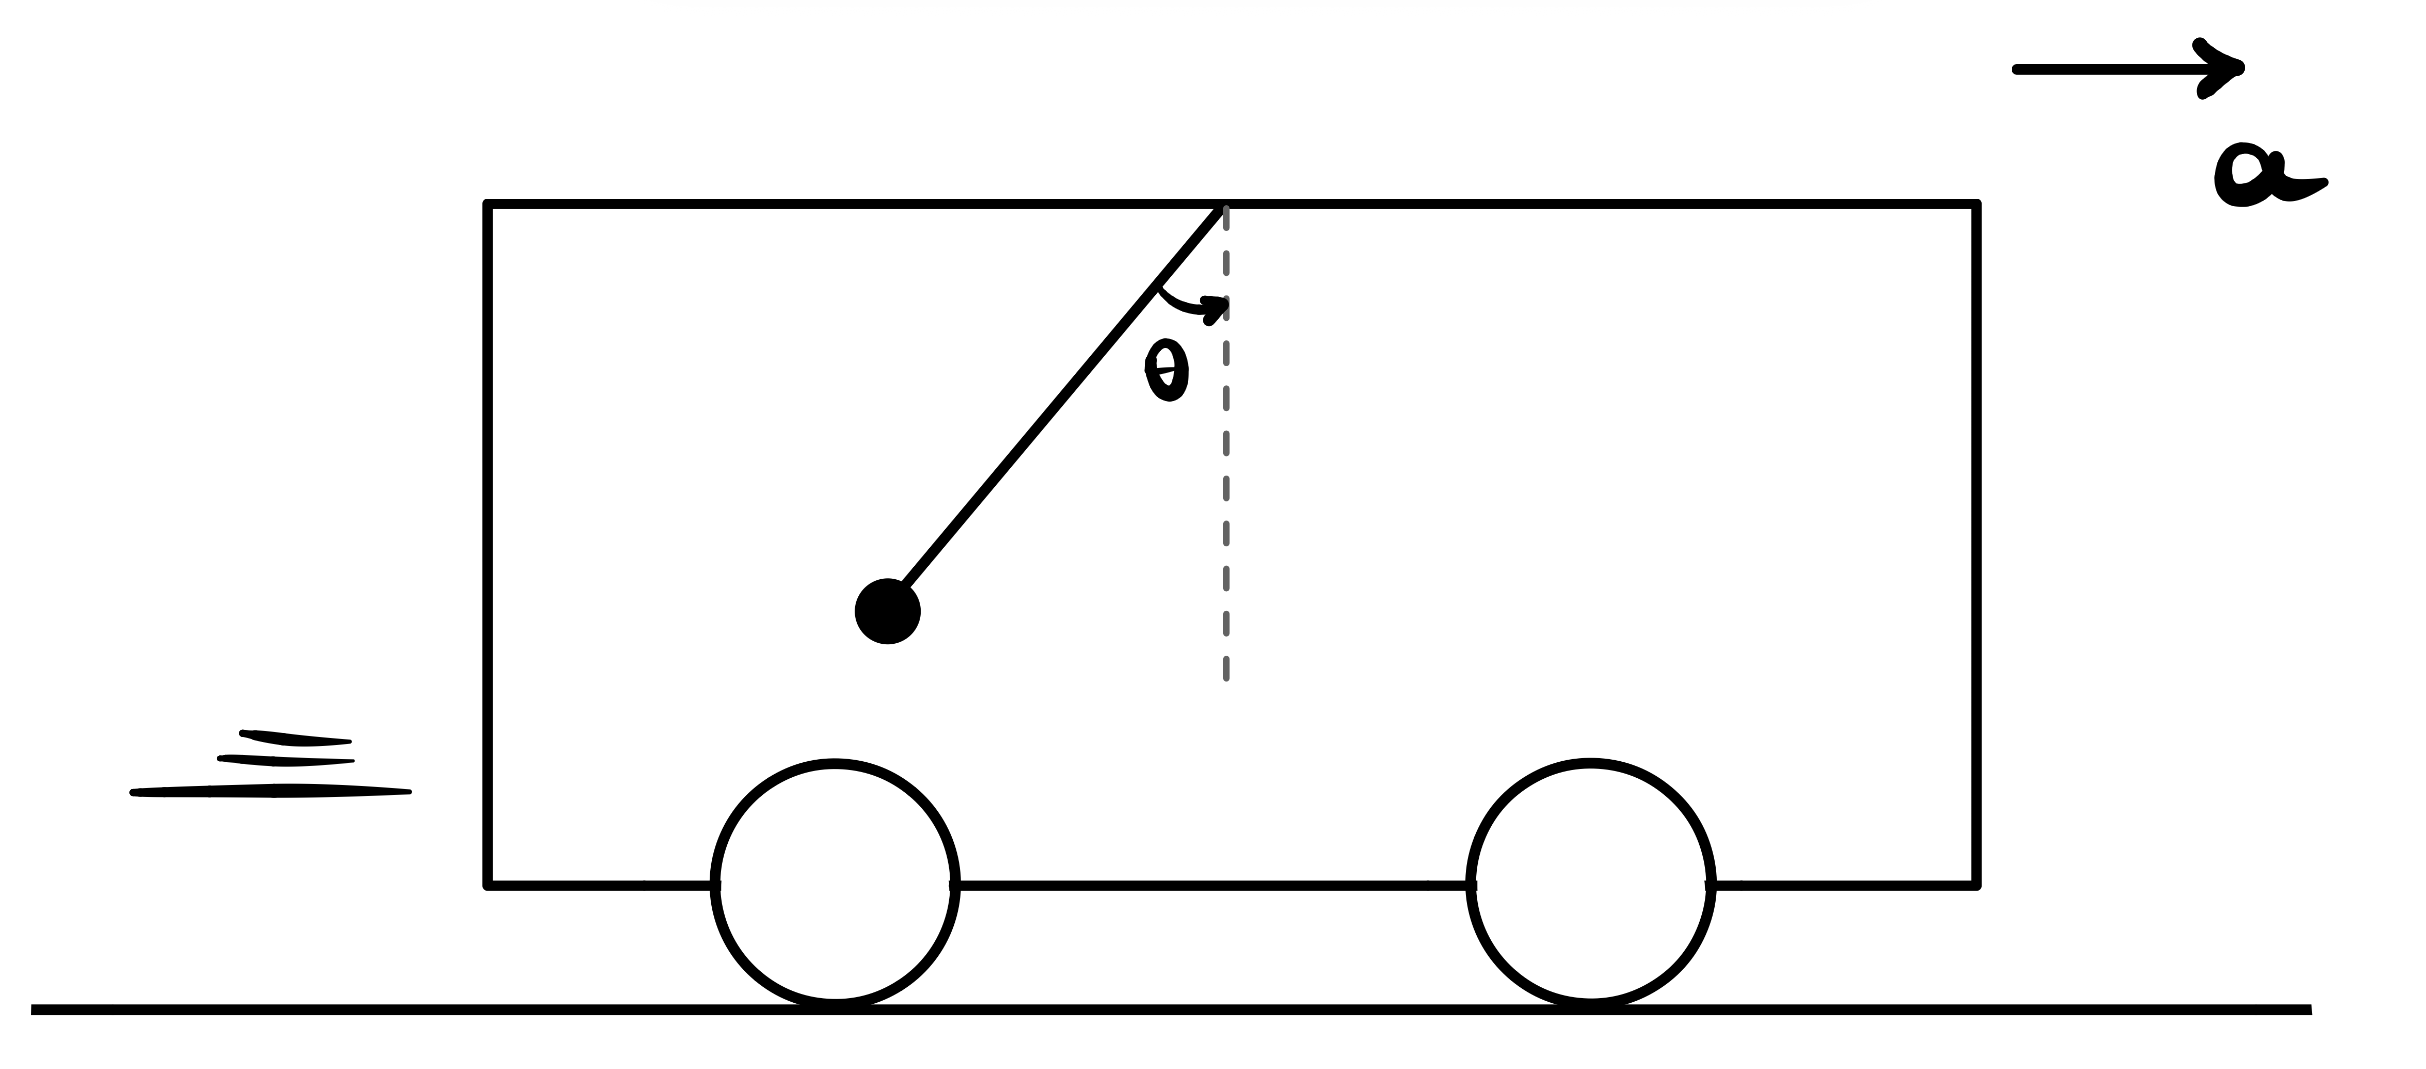
\includegraphics[width=0.5\linewidth]{imagensdinamicanewton/pendulodenewtonexemplo21.png}};
  \end{scope}
\end{tikzpicture}
\captionof{figure}{}
\label{fig_mec_pendulodenewtonexemplo21}
} 
\vspace{0.3cm}

\resolucao

Se o pêndulo permanece em repouso em relação ao vagão isso quer dizer que ele compartilha exatamente da mesma aceleração que o vagão. Lembre-se: o repouso é o movimento compartilhado. Dois corpos que executem exatamente o mesmo movimento terão a impressão de estarem em repouso um em relação ao outro. Assim, montamos o diagrama de forças na esfera do pêndulo, que aparece na Figura \ref{fig_mec_pendulodenewtonexemplo22}.

\vspace{0.3cm}
{
\centering
\begin{tikzpicture}
  \begin{scope}[blend mode=multiply]
    \node {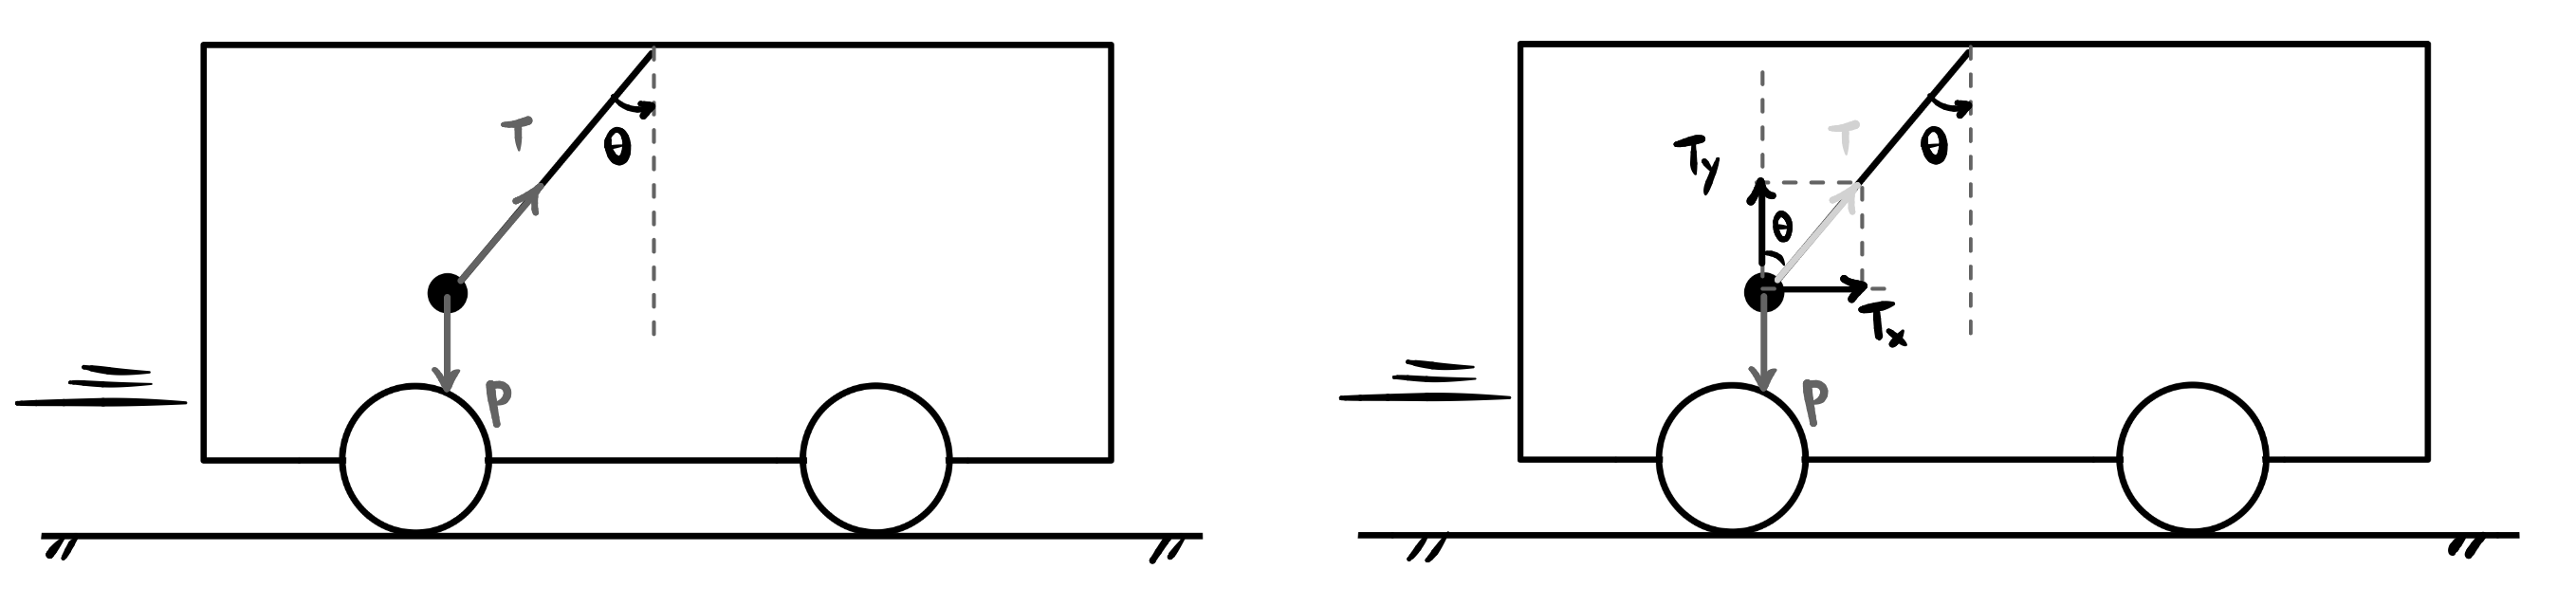
\includegraphics[width=0.99\linewidth]{imagensdinamicanewton/pendulodenewtonexemplo22.png}};
  \end{scope}
\end{tikzpicture}
\captionof{figure}{}
\label{fig_mec_pendulodenewtonexemplo22}
} 
\vspace{0.3cm}



Na vertical, como o vagão não se move, o pêndulo também não pode se mover. Logo, teremos:

$$ F_{\text{R}_y} = 0 \implies T_y = P \implies \boxed{T \cos \theta = mg.}$$

Na horizontal a resultante das forças deve produzir na massa a mesma aceleração $a$ que o vagão possui:

$$ F_{\text{R}_x} = m a_x \implies  \boxed{T \sin \theta =  ma.}$$

Dividindo as duas últimas equações seremos levados a

$$ \dfrac{\cancel T \sin \theta }{\cancel T \cos \theta } = \dfrac{\cancel ma}{\cancel mg} \implies \boxed{a = g \tan \theta.}$$

Logo, a aceleração do bloco deve ser exatamente igual a $a = g \tan \theta.$ Note que, para $\theta = 0,$ teremos $a=0.$ Ou seja, o pêndulo só fica alinhado com a vertical caso o vagão esteja em repouso ou em MRU -- as duas condições em que $a=0.$ Para que o pêndulo ficasse alinhado com a horizontal, isto é, $\theta = \sfrac{\pi}{2},$ seria preciso ter $a \to \infty.$ Isso mostra que quando mais intensa é a aceleração, mais próximo da horizontal o pêndulo fica, tendendo à horizontal para uma aceleração infinitamente grande. 

\end{exemplo}

\vspace{0.3cm}


\begin{exemplo}[Nível III]\label{exemplo_dinamicanewton_p=mg03}

Uma sonda espacial pousa num planeta sem atmosfera. O astronauta realiza
o seguinte experimento: arremessa verticalmente para cima um objeto de
massa $m$, a partir do solo, com velocidade inicial $v_0$
desconhecida. Duas grandezas são medidas com precisão:

\begin{itemize}
  \item altura máxima atingida pelo objeto acima do solo: $H$;
  \item tempo total de voo (do lançamento até o retorno ao solo): $T$.
\end{itemize}

\noindent Determine:

\begin{enumerate}
  \item [a)] o valor de $g$ naquele planeta, em função de $H$ e $T$;
  \item [b)] a velocidade inicial $v_0$ do lançamento, em função de $g$ e $T$;
  \item [c)] o peso do objeto nesse planeta, em função de $m$, $H$ e $T$;
  \item [d)] se o astronauta tivesse medido apenas $T$, sem registrar $H$,
  seria possível determinar $g$? Justifique.
\end{enumerate}

\resolucao



\noindent\textit{a)} Tomamos o eixo positivo para cima e a origem no solo. O objeto é
lançado com $v_0 > 0$ e sofre aceleração $-g$ (gravidade para baixo)
durante todo o voo. O problema se divide em duas etapas de cálculo:

\begin{enumerate}
    \item [(i)] Equação de Torricelli para cálculo da altura máxima:
    \begin{equation}
      0 = v_0^2 - 2gH \;\Longrightarrow\; v_0^2 = 2gH.  
      \label{eq_dinamicanewton_eqintermediariaexemplopeson31}
    \end{equation}
   



    \item [(ii)] Cálculo do tempo total de voo.

Como o movimento é simétrico (mesma aceleração constante, mesmo ponto
de partida e chegada, sem atrito), o tempo de subida é igual ao tempo
de descida. Portanto $T = 2\,t_{\text{sub}}$, onde $t_{\text{sub}}$ é
o tempo até a altura máxima. No ponto mais alto, $v = 0$, e da equação
$v = v_0 + at$ produz:

\begin{equation}
      0 = v_0 - g\,t_{\text{sub}}
  \;\Longrightarrow\;
  t_{\text{sub}} = \frac{v_0}{g}
  \;\Longrightarrow\;
  T = \frac{2v_0}{g}.
  \label{eq_dinamicanewton_eqintermediariaexemplopeson32}
\end{equation}

\end{enumerate}


Da Equação \eqref{eq_dinamicanewton_eqintermediariaexemplopeson32}: $v_0 = \dfrac{gT}{2}$. Substituindo na Equação \eqref{eq_dinamicanewton_eqintermediariaexemplopeson31}:

\[
  \left(\frac{gT}{2}\right)^2 = 2gH
  \;\Longrightarrow\;
  \frac{g^2 T^2}{4} = 2gH
  \;\Longrightarrow\;
  \boxed{g = \frac{8H}{T^2}.}
\]

\medskip
\noindent\textit{b)} Com $g$ determinado, obtemos $v_0$ pela Equação \eqref{eq_dinamicanewton_eqintermediariaexemplopeson32}:

\[
  \boxed{v_0 = \frac{gT}{2} = \frac{4H}{T}.}
\]

\medskip
\noindent\textit{c)} O peso do objeto no planeta:

\[
  \boxed{P = mg = \frac{8mH}{T^2}.}
\]

\noindent O peso depende das duas medidas experimentais $H$ e $T$, e
cresce com $H$ (quanto mais alto o objeto sobe, mais forte é a
gravidade local)\footnote{Um pouco estranho este resultado, não? O leitor consegue perceber a razão de sê-lo?} e decresce com $T^2$ (quanto mais tempo o objeto
permanece no ar, mais fraca é a gravidade que o puxa de volta). O
objeto tem a mesma \emph{massa} $m$ em qualquer lugar do universo;
o que muda é o \emph{peso}, que é ditado pelo campo gravitacional
local.

\medskip
\noindent\textit{d)} Se apenas $T$ fosse conhecido, a equação
disponível seria $T = 2v_0/g$, ou seja:

\[
  \frac{v_0}{g} = \frac{T}{2}.
\]

\noindent Esta é uma relação entre duas incógnitas, não uma equação
que as determina individualmente. Há infinitas combinações de $g$ e
$v_0$ que satisfazem $v_0/g = T/2$ para um dado $T$: basta tomar
qualquer $g > 0$ e definir $v_0 = gT/2$. Sem a segunda medida $H$
--- ou qualquer outra informação independente --- o sistema é
indeterminado. Dois dados são necessários para determinar duas
incógnitas.



\end{exemplo}




\begin{secnivel}[Lei de Hooke]{I}{Lei de Hooke}
  
  \eqLdois{exp}{eq_dinamicanewton_leihooke}{F = kx}

\end{secnivel}







\secgfe{De onde vem} 

A lei de Hooke nos diz qual é a força $F$ exercida por uma mola de constante elástica $k$ quando deformada de $x$ em relação ao seu comprimento inicial. Como mostra a Figura \ref{fig_dinamicanewton_hooke01}, quando distendemos uma mola, a sua tendência natural é retornar à posição de equilíbrio. Sendo assim, manifesta-se nas extremidades da mola uma força que a puxa de volta para sua posição inicial.

\vspace{0.3cm}
{
\centering
\begin{tikzpicture}
  \begin{scope}[blend mode=multiply]
    \node {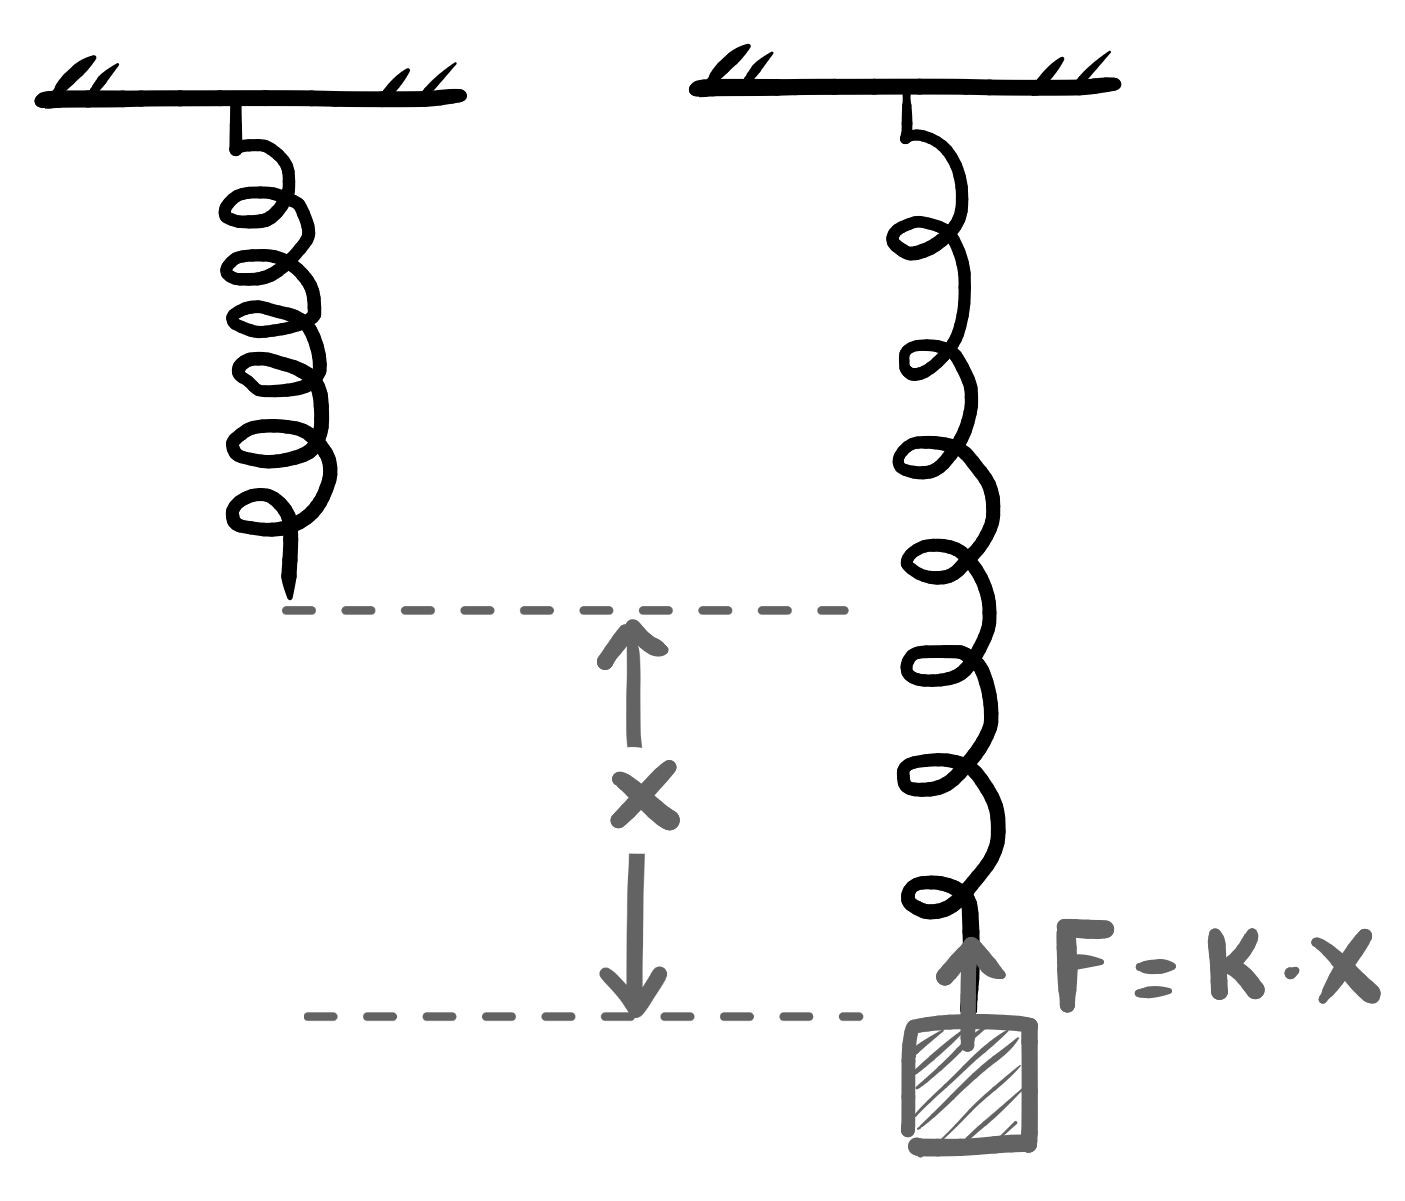
\includegraphics[width=0.3\linewidth]{imagensdinamicanewton/leihooke1.png}};
  \end{scope}
\end{tikzpicture}
\captionof{figure}{Ao ser distendida a mola tende a voltar para sua posição inicial. Com isso, surgem forças nas suas extremidades puxando-a de volta para sua posição natural.}
\label{fig_dinamicanewton_hooke01}
} 

\vspace{0.3cm}

A Equação \eqref{eq_dinamicanewton_leihooke} diz que tal força é diretamente proporcional à deformação $x$ da mola. Este é um fato obtido experimentalmente: para uma certa mola, pode-se avaliar, para diferentes deformações, qual é o valor da força que se manifesta em sua extremidade. Ao fazer isso, o experimento irá nos fornecer alguns dados, mostrados no gráfico da primeira imagem da Figura \ref{fig_dinamicanewton_hooke03}. Os dados experimentais indicam que a relação entre $F$ e $x$ é linear: uma relação de proporção direta, do tipo $y(x)=ax,$ ou, no nosso caso, $F(x)=kx.$

\vspace{0.3cm}
{
\centering
\begin{tikzpicture}
  \begin{scope}[blend mode=multiply]
    \node {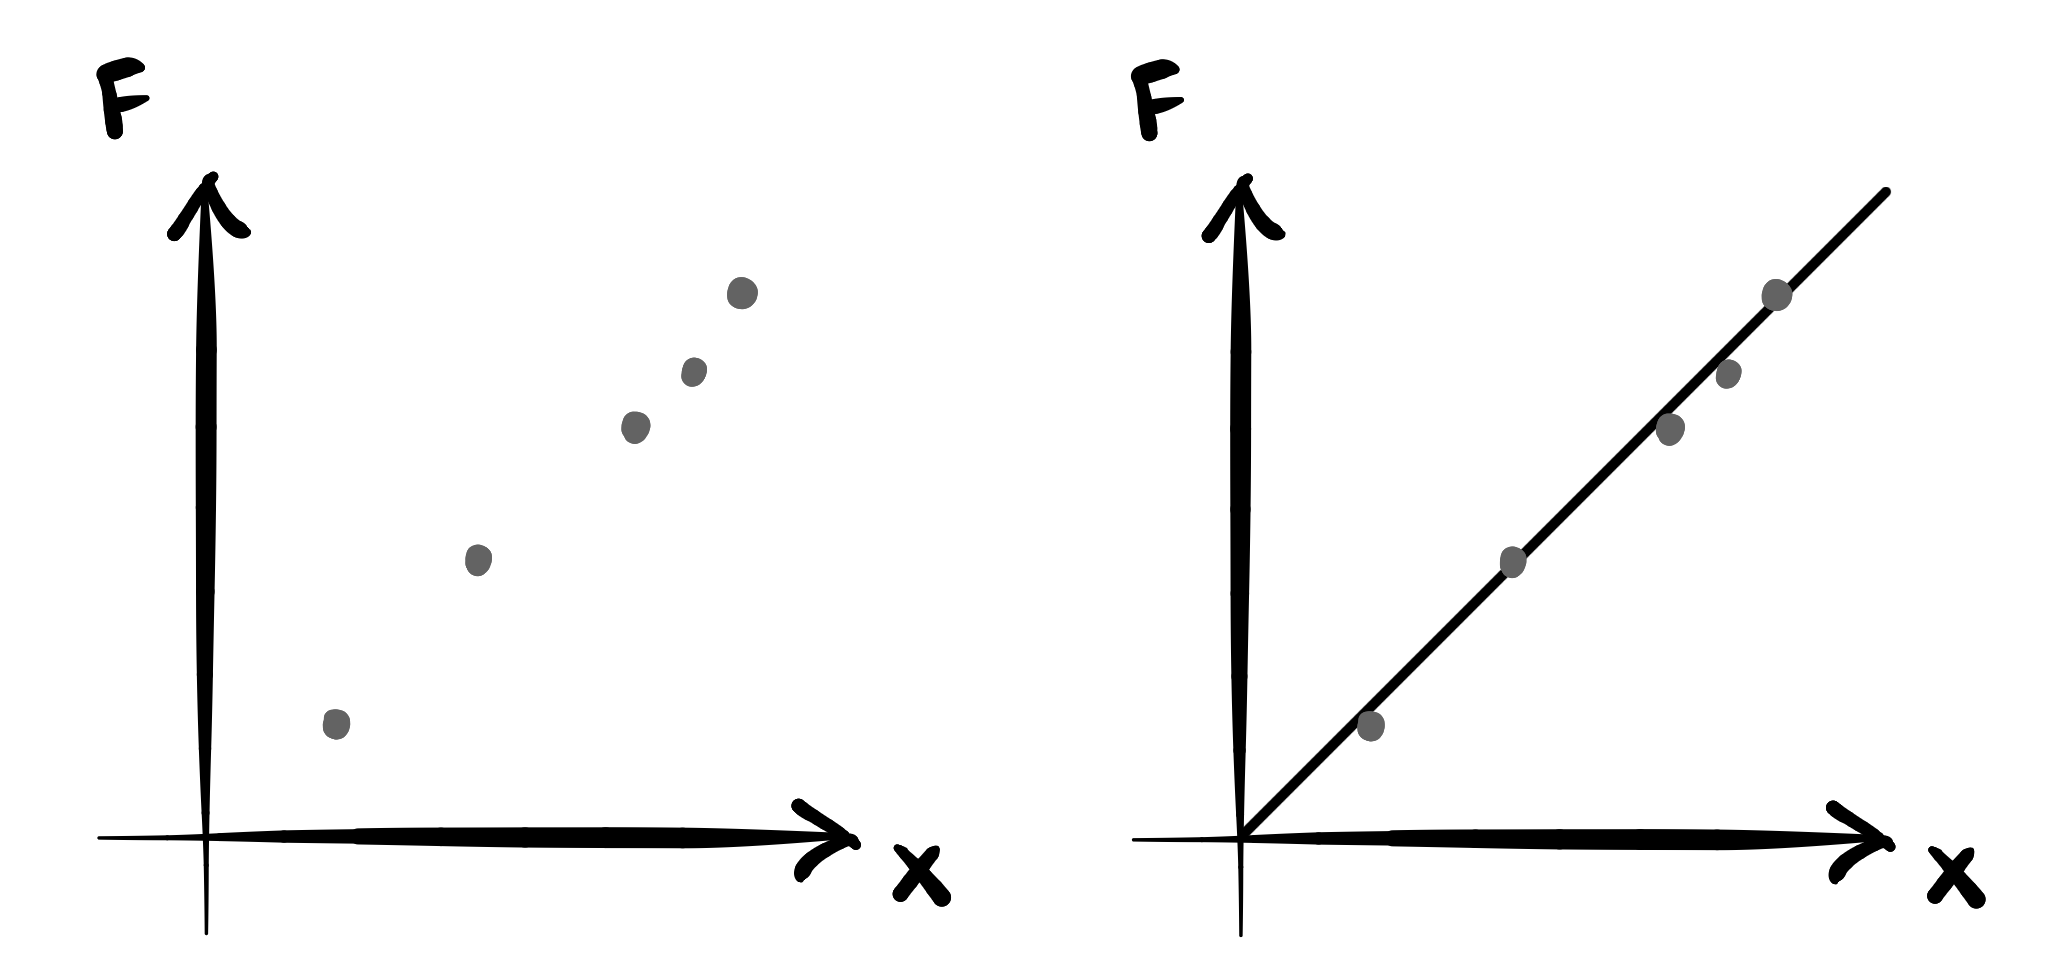
\includegraphics[width=0.5\linewidth]{imagensdinamicanewton/leihooke3.png}};
  \end{scope}
\end{tikzpicture}
\captionof{figure}{Ao plotar as forças $F$ que se manifestam na extremidade da mola para diferentes deformações $x$ encontramos que a relação entre essas duas grandezas é linear.}
\label{fig_dinamicanewton_hooke03}
}
\vspace{0.3cm}


É comum também, em algumas literaturas, apresentar a Equação \eqref{eq_dinamicanewton_leihooke} na forma $F=-kx.$ Neste caso, o sinal negativo entra ali apenas para indicar que a força terá sentido contrário ao deslocamento da mola. Como mostra a Figura \ref{fig_dinamicanewton_hooke01}, ao puxar a mola para baixo, a força elástica irá se manifestar para cima, puxando a mola de volta para sua posição inicial.




\secgfe{Onde é usada}

A Equação \eqref{eq_dinamicanewton_leihooke} será usada, naturalmente, em qualquer problema que envolva uma mola/elástico; como em um estilingue ou um arco e flecha. Cabe, contudo, trazermos luz ao leitor para alguns contextos em que as molas aparecem de forma implícita.

Um deles refere-se a um contexto bem interessante. Considere o seguinte: se a força peso de um corpo, como vimos na Equação \eqref{eq_dinamicanewton_peso=mg}, é a força de interação gravitacional entre a terra e o corpo, como podemos medi-la? A resposta a essa pergunta está relacionada a molas e à Equação \eqref{eq_dinamicanewton_leihooke}.

A Figura \ref{fig_dinamicanewton_hooke02} mostra, de forma simples, a estrutura de uma balança. Tal objeto funciona com um sistema de diversas pequenas molas -- simplificado por uma única mola na figura. Ao subir na balança, por conta da sua força peso, o indivíduo será puxado contra o chão, o que o fará empurrar a mola para baixo, comprimindo-a.

\vspace{0.3cm}
{
\centering
\begin{tikzpicture}
  \begin{scope}[blend mode=multiply]
    \node {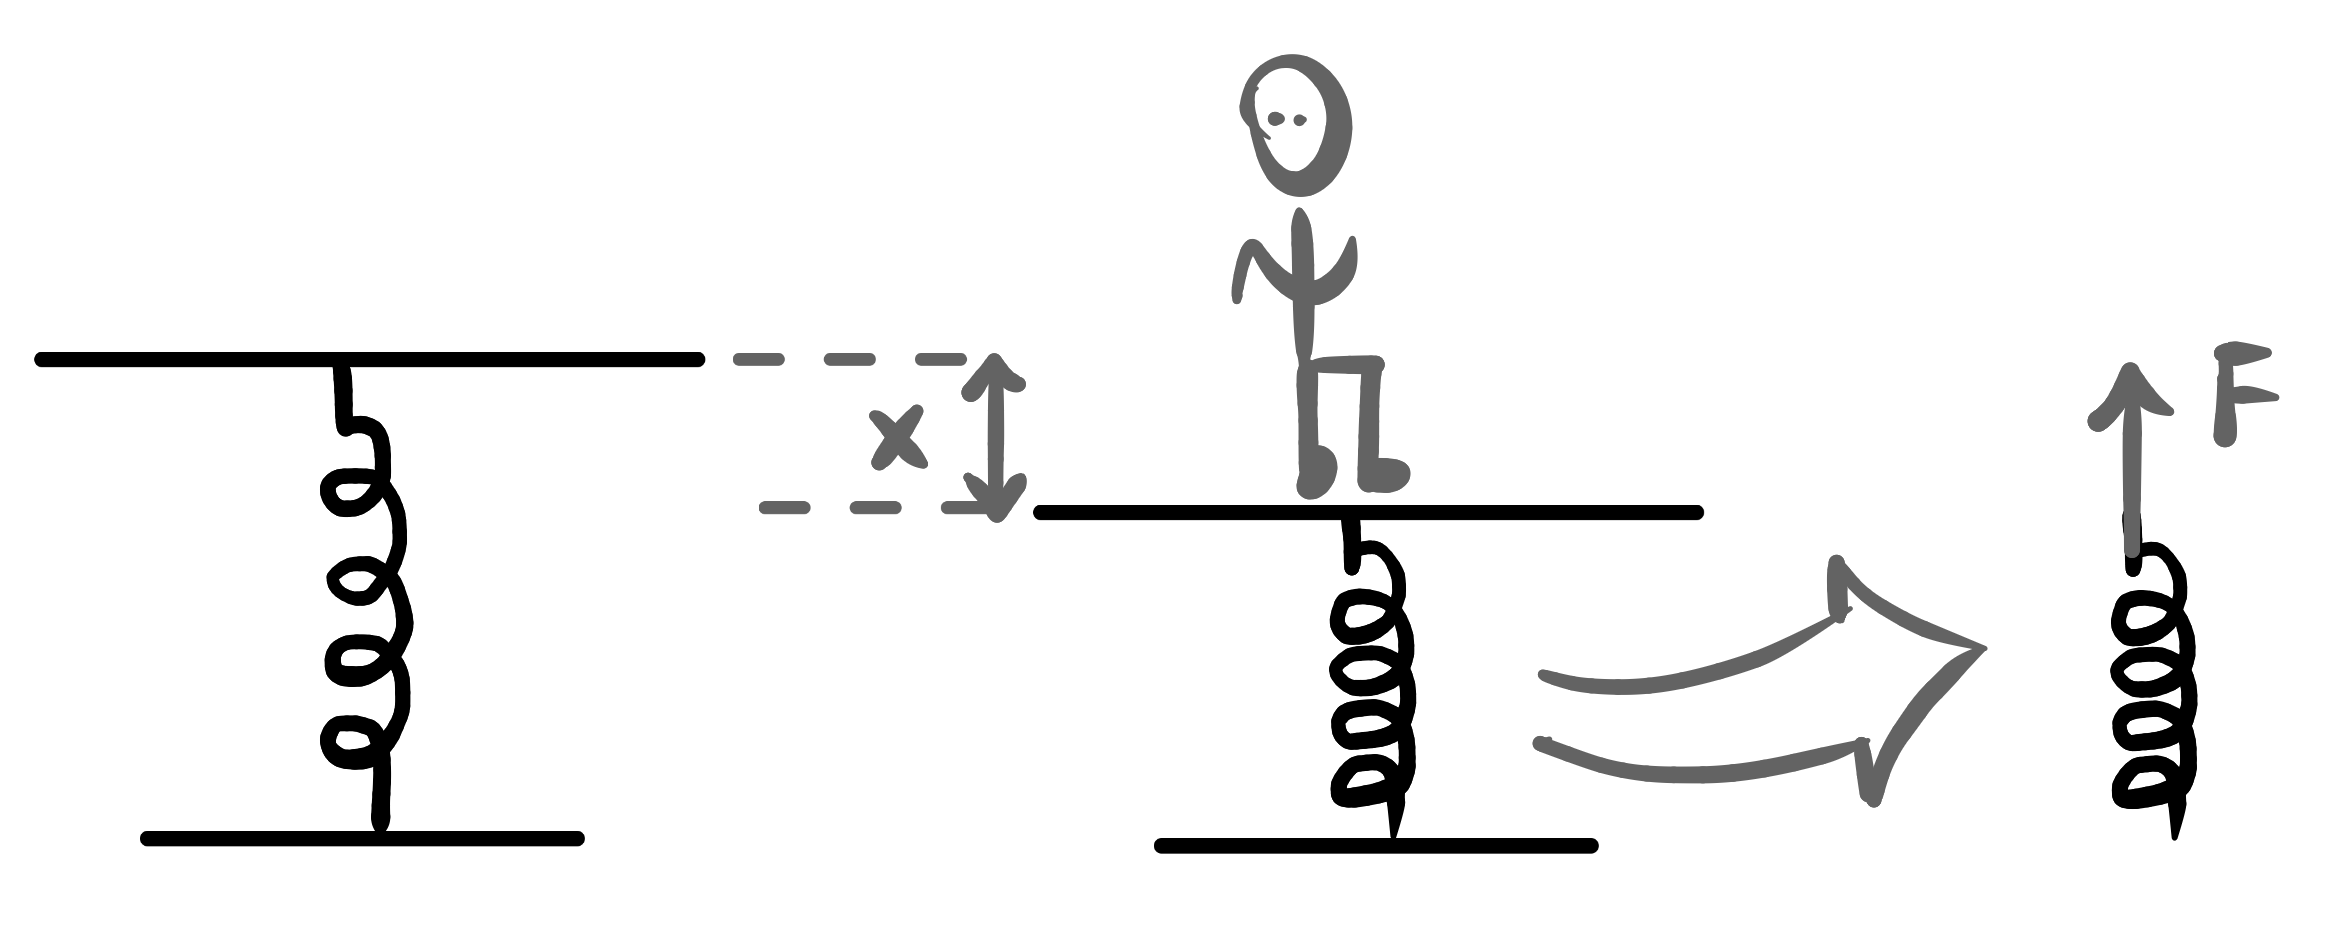
\includegraphics[width=0.5\linewidth]{imagensdinamicanewton/leihooke2.png}};
  \end{scope}
\end{tikzpicture}
\captionof{figure}{A balança não mede a sua força peso: ela mede o quanto as molas foram comprimidas.}
\label{fig_dinamicanewton_hooke02}
} 

\vspace{0.3cm}

Ao atingir sua nova posição de equilíbrio,\footnote{Situação em que a mola terá parado de ser comprimida, ou seja, a força elástica, empurrando o indivíduo para cima, terá que ser igual ao seu peso, que empurra a mola para baixo -- nessa situação cessa a deformação da mola.} a mola terá se deformado de um tanto $x,$ o que pode ser facilmente medido, como destaca a figura.

Ora, sabendo qual é a mola usada na construção da balança, saberemos qual é o valor da sua constante elástica $k,$ que é uma propriedade intrínseca da mola. Munidos desses valores, podemos usar a Lei de Hooke para encontrar o valor da força elástica:

$$ F = kx,$$

\noindent haja vista que o valor de $x$ foi medido e o valor de $k$ é conhecido. Logo, com isso, teremos a força elástica $F$ com que a mola empurra o indivíduo para cima. Ora, se o indivíduo está em equilíbrio, isto é, a mola não está mais sendo comprimida, isso significa que a força que o empurra para cima -- a força elástica -- deve ser exatamente igual, em módulo, ao valor do seu peso $P$, que é a força que o puxa para baixo: se as forças se anularem o menino não irá comprimir a mola para além da sua compressão atual. Assim, teremos:

$$ F=P,$$

\noindent e, como a força elástica $F$ pode ser medida, conseguimos, indiretamente, obter o peso do indivíduo. Como $P=mg,$ basta informar para o sistema eletrônico o valor da gravidade $g$ na superfície da Terra e programar o visor para pegar a força obtida e dividi-la por tal valor, de modo a obter a massa do indivíduo:

$$ P =mg \implies m = \dfrac{P}{g}.$$

Perceba como é engenhoso o sistema da balança, uma vez que

\begin{enumerate}
    \item [(i)] A balança não mede \textbf{nunca} o seu peso $P$. O que ela consegue medir é um comprimento geométrico: o quando a mola foi deformada. Munidos deste valor e conhecendo a constante elástica da mola, a Equação \eqref{eq_dinamicanewton_leihooke} nos permite obter a força elástica que a mola exerce, empurrando a base com o menino para cima, a fim de voltar à sua posição inicial. 

    Se, neste ponto, o sistema estiver em equilíbrio: o menino não está descendo, comprimindo mais a mola; nem subindo, então significa que a sua força peso que o puxa para baixo é igual à força elástica que o empurra para cima: $F=P.$ Logo, obtemos o valor da força peso do indivíduo, \textbf{de forma indireta: o que medimos de fato é uma deformação, que nos permite computar a força elástica na mola. Pelo fato de ela, neste contexto, ser igual ao peso, conseguimos obter o peso do indivíduo}.

    \item [(ii)] Ainda assim, no final, o que teríamos não é a massa do indivíduo, mas sim o valor do seu peso, que foi medido de forma indireta. Desse modo, seria necessário informar ao sistema da balança o valor da gravidade $g$ no local onde ela se encontra e programá-la para pegar o valor obtido e dividir por $g$, pois, pela Equação \eqref{eq_dinamicanewton_peso=mg}, a massa é a razão entre a força peso e a aceleração da gravidade: $m=\sfrac{P}{g}.$
\end{enumerate}



Perceba que esse tipo de mecanismo constitui uma nova ferramenta para medir forças: as forças podem ser medidas com base na deformação de molas. Digamos que queremos avaliar quem é mais forte: Aristóteles ($A)$ ou Bohr ($B$). Podemos pedir para que Aristóteles puxe uma mola, fixa em uma parede, por exemplo, com sua força máxima $F_A.$

Em seguida, pedimos que Bohr puxe um sistema com duas molas idênticas, uma ao lado da outra, com sua força máxima $F_B$. Se constatarmos que Bohr consegue gerar a mesma deformação que Aristóteles, podemos dizer que ele é duas vezes mais forte, uma vez que teve que distender duas molas para tal. Isto é, $F_B= 2F_A$, como mostra a Figura \ref{fig_dinamicanewton_hooke04}. Tal dispositivo é conhecido como dinamômetro e é usado para medir forças com base na lei de Hooke.

\vspace{0.3cm}

{
\centering
\begin{tikzpicture}
  \begin{scope}[blend mode=multiply]
    \node {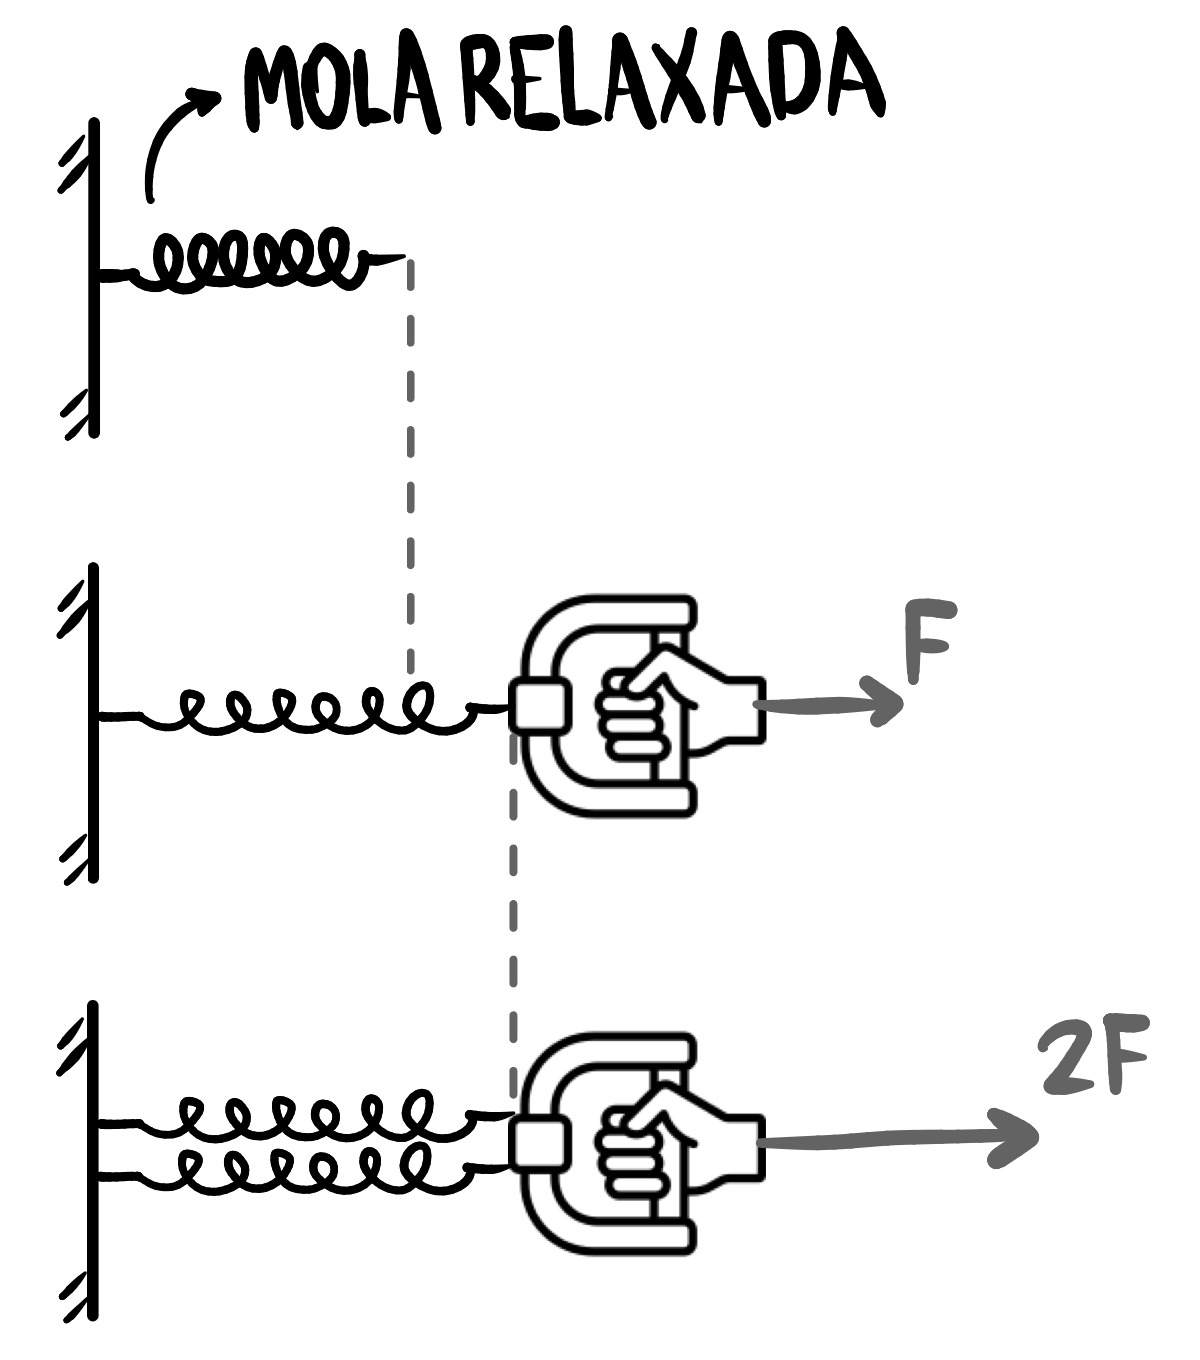
\includegraphics[width=0.35\linewidth]{imagensdinamicanewton/leihooke4.png}};
  \end{scope}
\end{tikzpicture}
\captionof{figure}{O mecanismo do dinamômetro.}
\label{fig_dinamicanewton_hooke04}
} 
\vspace{0.3cm}


\secgfe{Erros comuns}


Talvez o erro mais comum aqui seja confundir a deformação $x$ da mola com o seu comprimento natural $L.$ Se tivermos uma mola de constante elástica $k = 10$ N/cm, cujo comprimento natural -- isto é, o comprimento da mola relaxada, sem estar comprimida ou esticada -- é de 30 cm, qual é a força elástica se nós a esticarmos de $3$ cm? Alguns estudantes, neste caso, tendem a considerar como valor de $x$ para o cálculo na lei de Hooke o valor de 30 cm, ou de 33 cm. Contudo, o cálculo correto é

$$ F = kx = \dfrac{10 \text{ N}}{\text{ cm}} \cdot 3 \text{ cm} = 30 \text{ N.}$$

Perceba que o comprimento inicial da mola de 30 cm é irrelevante -- ele poderia ser de 50 cm, de 75 cm ou qualquer outro valor. O que importa para o cálculo da força elástica é a deformação $x$ da mola: o quanto ela foi esticada ou comprimida a partir da sua posição relaxada. Logo, o comprimento inicial $L$ da mola é irrelevante para o cálculo da força elástica.
 


\secgfe{Observações}

A constante $k$, chamada de constante elástica da mola, é uma grandeza que irá depender de características específicas daquela mola, nos dizendo quantos Newtons de força são necessários para deformar a mola de uma certa quantidade:

$$ [\text{k}] = \dfrac{[\text{F}]}{ [\text{x}]}  = \dfrac{\text{N}}{\text{m}}. $$

Uma mola de constante elástica $k = 80 \text{ N}/ $m é uma mola que exige 80 N de força para que ela seja esticada (ou comprimida) de exatamente 1 metro.


\vspace{0.3cm}

\begin{exemplo}[Nível I]\label{exemplo_newton_hooke01}

Considere a situação, como na Figura \ref{fig_dinamicanewton_hooke01}, que um bloco massa $m=4$ kg foi pendurado na extremidade de uma mola de constante elástica $k=50$ N/m.

Se o bloco fica em repouso após a distensão da mola, de quanto ela foi distendida?

\resolucao

No bloco atuam duas forças: o peso, verticalmente para baixo, e a força elástica, para cima. Se ele fica em repouso então as forças devem se anular:

$$ F_R = 0 \implies P = F \implies mg = kx \implies x = \dfrac{mg}{k}=\dfrac{4 \cdot 10}{50}= 0.8 \text{ m.}$$




\end{exemplo}



\vspace{0.3cm}

\begin{exemplo}[Nível II]\label{exemplo_newton_hooke02}

Um bloco de massa $m=5$ kg é amarrado na extremidade de uma mola. Ao empurrar o bloco 10 cm contra a parede, como mostra a Figura \ref{fig_dinamicanewton_hookeex021}, percebe-se que sua aceleração, assim que ele é solto, é de $2$ m/s$^2.$ Encontre a constante elástica da mola.




\vspace{0.3cm}
{
\centering
\begin{tikzpicture}
  \begin{scope}[blend mode=multiply]
    \node {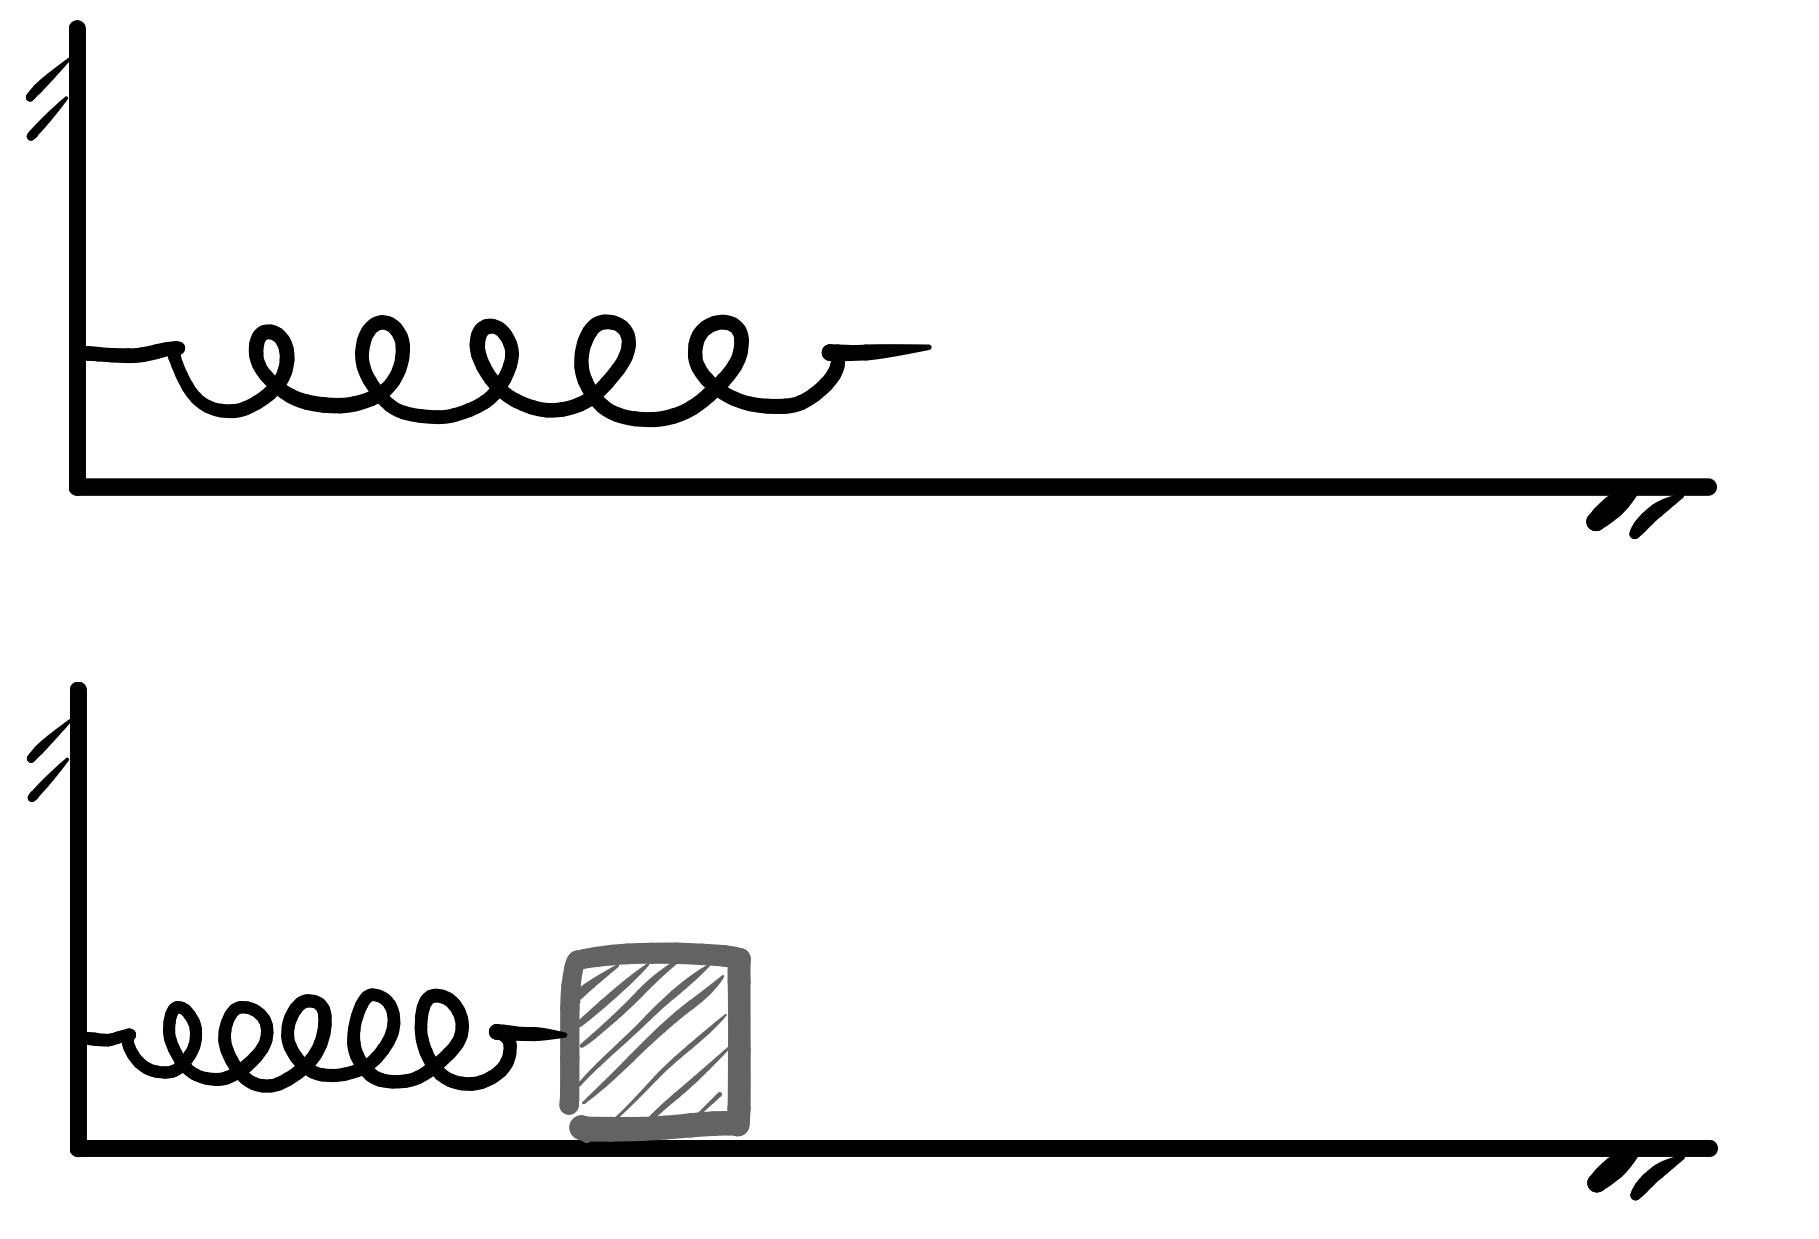
\includegraphics[width=0.35\linewidth]{imagensdinamicanewton/hookeex021.png}};
  \end{scope}
\end{tikzpicture}
\captionof{figure}{}
\label{fig_dinamicanewton_hookeex021}
} 
\vspace{0.3cm}


\resolucao

Como mostra a Figura \ref{fig_dinamicanewton_hookeex022}, analisando as forças na horizontal, a força resultante atuando no bloco será a própria força elástica. Logo, usando a lei de Hooke e a Segunda Lei de Newton, teremos

$$ F_R = F_{EL} \implies ma = kx \implies k = \dfrac{ma}{x} = \dfrac{5 \cdot 2}{0.1} = 100 \text{ N/m}.$$


\vspace{0.3cm}
{
\centering
\begin{tikzpicture}
  \begin{scope}[blend mode=multiply]
    \node {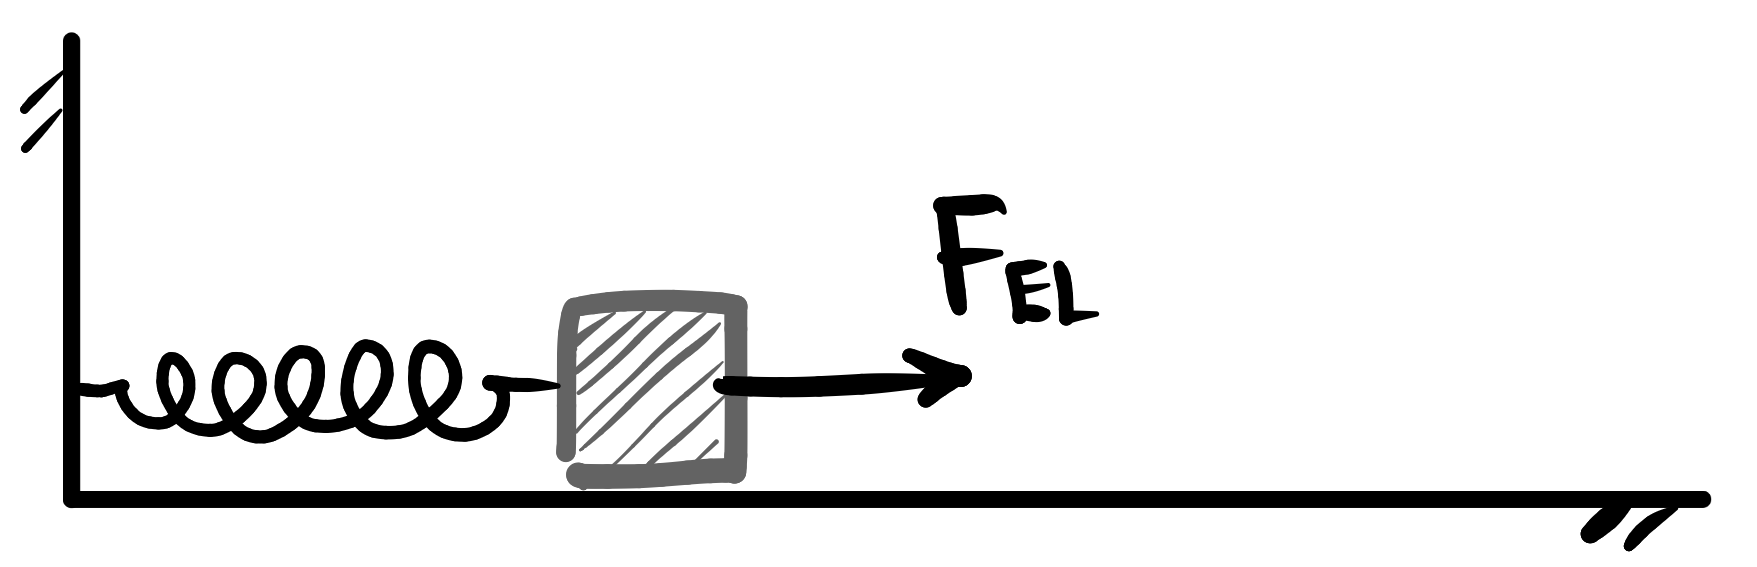
\includegraphics[width=0.35\linewidth]{imagensdinamicanewton/hookeex022.png}};
  \end{scope}
\end{tikzpicture}
\captionof{figure}{}
\label{fig_dinamicanewton_hookeex022}
} 
\vspace{0.3cm}

Note que convertemos a deformação $x$ da mola de centímetros para metros, a fim de inserir todas as informações na equação no SI e garantir que o resultado sairia, também, no SI.

\end{exemplo}


\vspace{0.3cm}



\begin{exemplo}[Nível III]\label{exemplo_newton_hooke03}

Considere duas molas de mesmo comprimento inicial e constantes elásticas $k_1$ e $k_2$. Mostre que

\begin{enumerate}
    \item [(a)] ao associar as molas em paralelo, isto é, de modo que a deformação delas seja a mesma, o sistema pode ser substituído por uma única mola de constante $k_{eq}=k_1+k_2.$

     \item [(b)] ao associar as molas em série, isto é, de modo que a força em cada uma delas seja a mesma, o sistema pode ser substituído por uma única mola de constante $k_{eq}$ dada por $\sfrac{1}{k_{eq}}= \sfrac{1}{k_1}+\sfrac{1}{k_2}.$
\end{enumerate}

\resolucao


\noindent a) Molas em paralelo — mesma deformação.

Quando as duas molas estão em paralelo, uma força externa $F$ é
aplicada ao sistema e ambas se deformam do mesmo valor $x$ (pois estão
fixadas nos mesmos dois pontos). Cada mola reage individualmente com
sua própria força:

\[
  F_1 = k_1\,x \qquad \text{e} \qquad F_2 = k_2\,x.
\]




\vspace{0.3cm}
{
\centering
\begin{tikzpicture}
  \begin{scope}[blend mode=multiply]
    \node {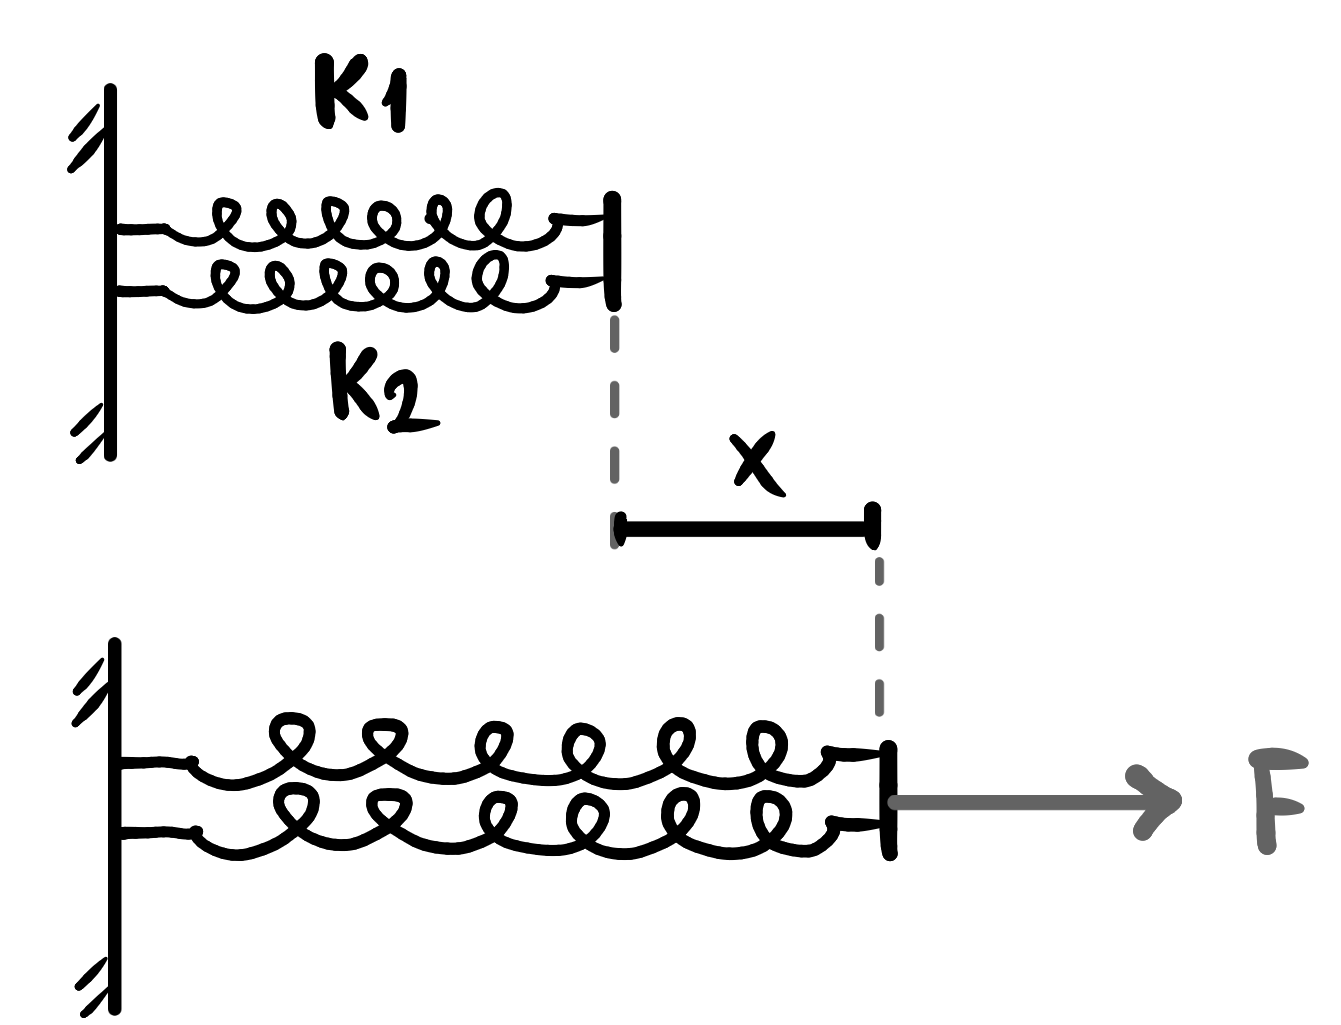
\includegraphics[width=0.40\linewidth]{imagensdinamicanewton/associacaodemolas1.png}};
  \end{scope}
\end{tikzpicture}
\captionof{figure}{Associação de molas em paralelo.}
\label{fig_dinamicanewton_associacaodemolas1}
} 
\vspace{0.3cm}


\noindent A força total que as molas exercem deve ser capaz de anular a força externa $F$ para que a mola fique em equilíbrio naquela posição. Logo:

\[
  F = F_1 + F_2 = k_1\,x + k_2\,x = (k_1 + k_2)\,x.
\]

\noindent Uma mola equivalente, por definição, satisfaz $F = k_{eq}\,x$. Ou seja, quando submetida a uma mesma deformação $x$ que o conjunto das outras duas, ela faz a mesma força total $F$ feita pelo sistema. Comparando com a expressão acima:


$$ F = k_{eq}\,x = (k_1 + k_2)\,x,$$

\noindent de onde segue que 

\[
  \boxed{k_{eq} = k_1 + k_2.}
\]

\noindent O resultado é intuitivo: em paralelo, as molas ``somam
esforços'' para resistir à mesma deformação, de modo que o sistema é
mais rígido do que qualquer uma das molas individualmente. Assim, podemos substituir o sistema de duas molas da Figura \ref{fig_dinamicanewton_associacaodemolas1} por uma única mola, de constante elástica $k_{eq} = (k_1 + k_2)$, e, quando submetida àquela mesma força $F,$ nossa mola sofrerá a mesma deformação $x$ que o sistema inicial sofria.

\bigskip
\noindent b) Molas em série — mesma força.

Quando as molas estão em série, a mesma força $F$ percorre toda a
cadeia --- se assim não fosse, algum trecho do sistema estaria
acelerando, o que contraria o equilíbrio estático. 

\vspace{0.3cm}
{
\centering
\begin{tikzpicture}
  \begin{scope}[blend mode=multiply]
    \node {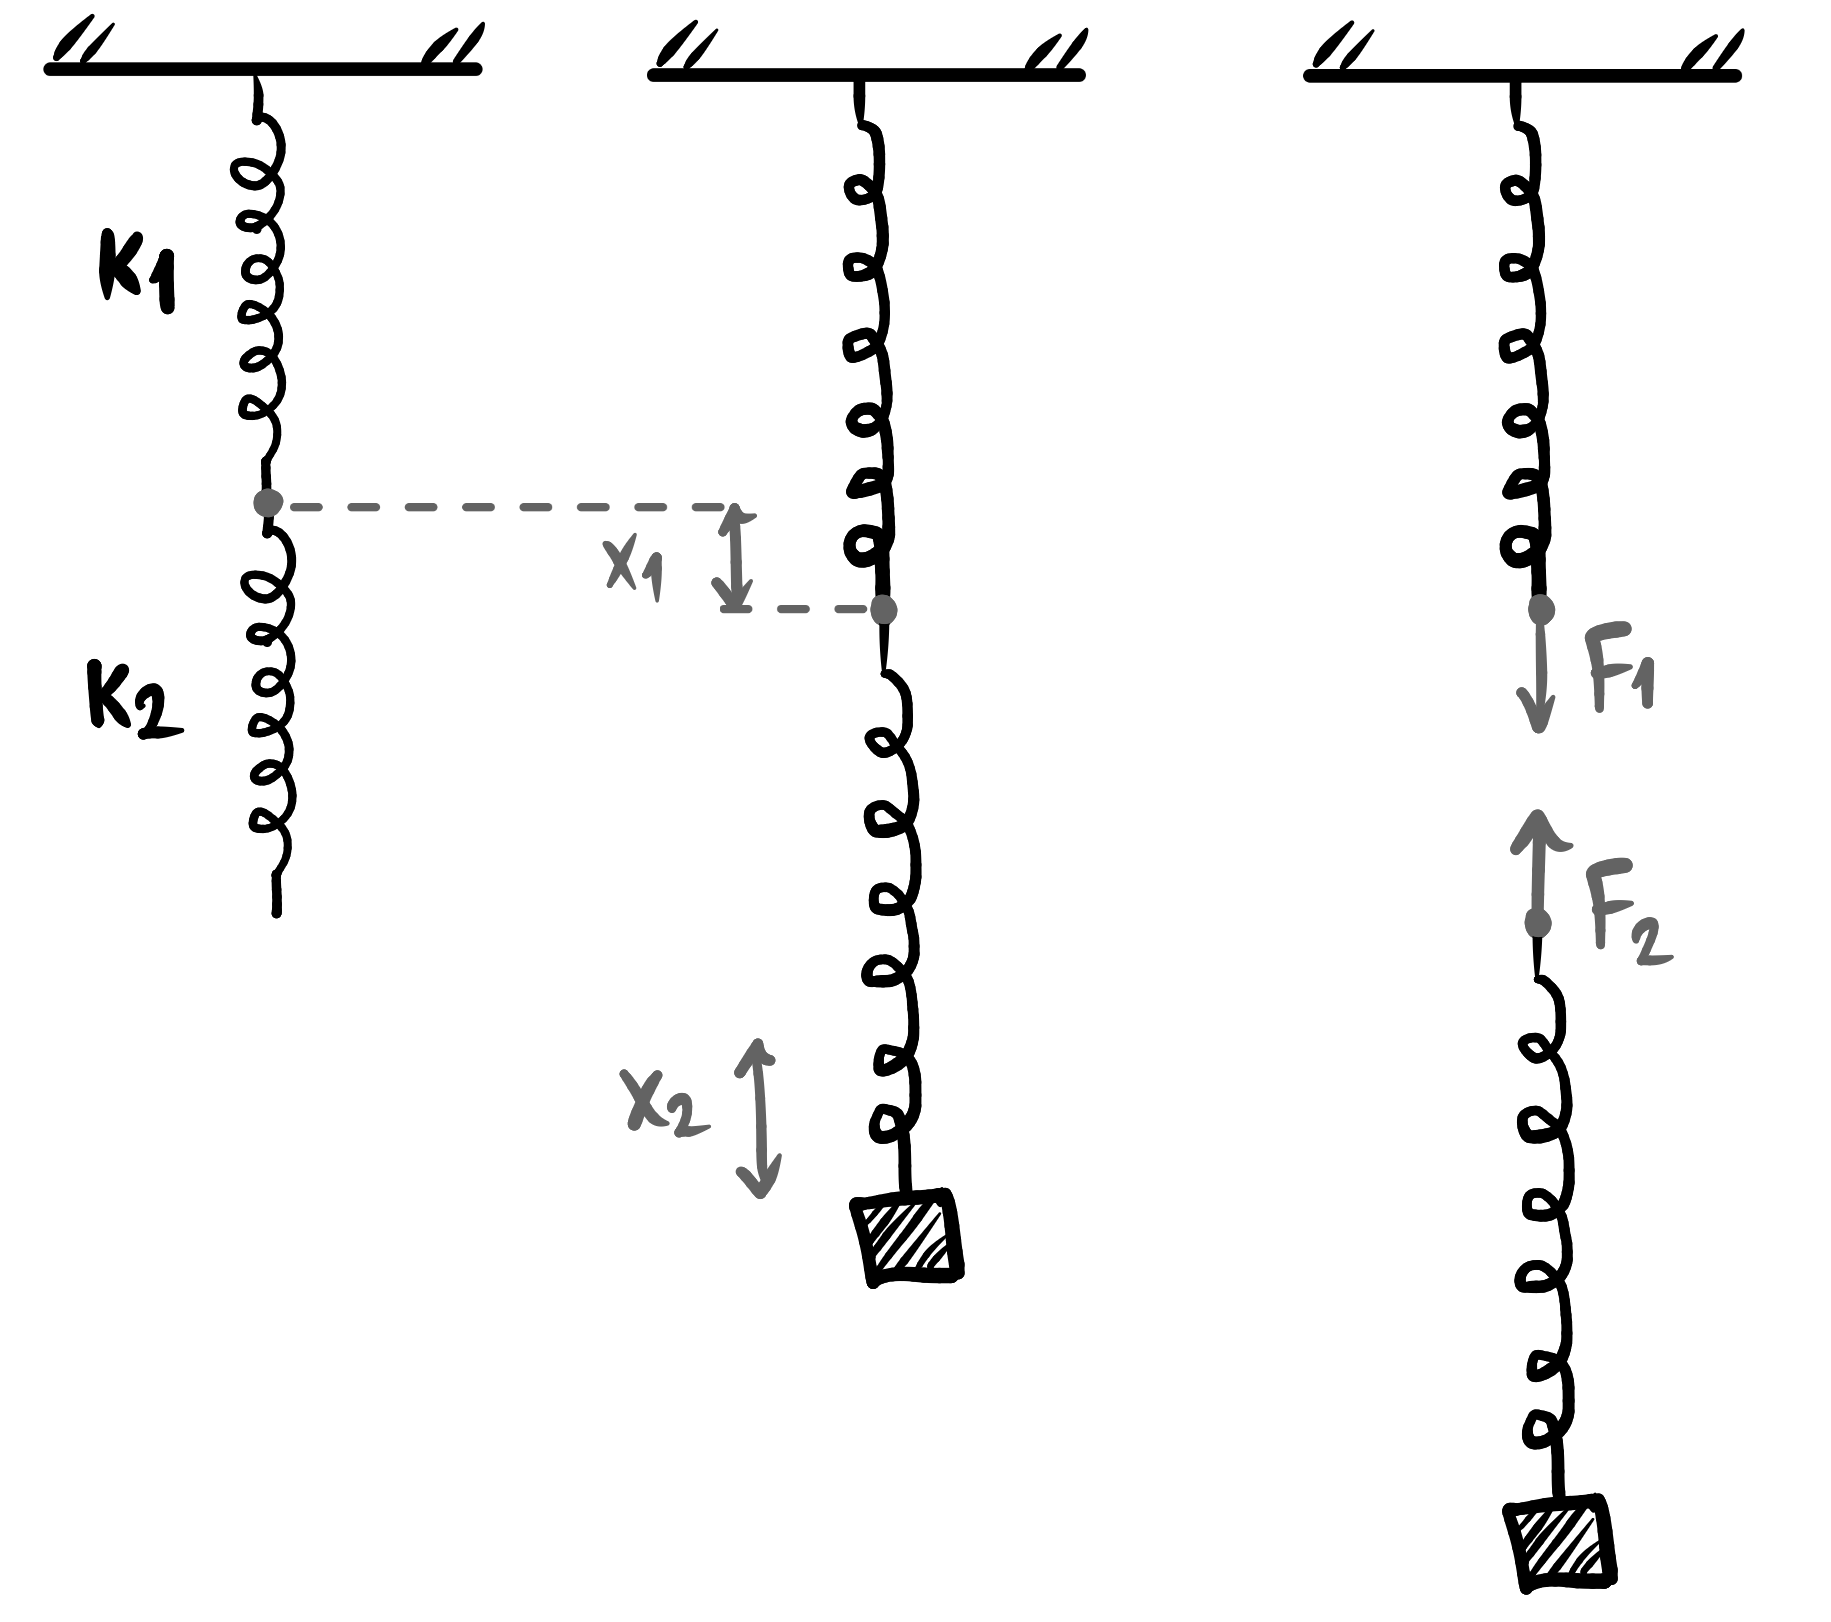
\includegraphics[width=0.55\linewidth]{imagensdinamicanewton/associacaodemolas2.png}};
  \end{scope}
\end{tikzpicture}
\captionof{figure}{Associação de molas em série.}
\label{fig_dinamicanewton_associacaodemolas2}
} 
\vspace{0.3cm}

A terceira imagem da Figura \ref{fig_dinamicanewton_associacaodemolas2} ilustra isso: a força $F_1$ com que a mola 1 puxa a mola 2, no ponto de junção, deve ser igual à força $F_2$ com que a mola 2 puxa a mola 1, para que o sistema não esteja acelerado naquele ponto. Logo:

$$ F_1 = F_2 = F\implies k_1 x_1 = k_2x_2 = F \implies \boxed{x_1 = \dfrac{F}{k_1} \quad \text{ e } \quad x_2 = \dfrac{F}{k_2}.}$$


\noindent A deformação total do sistema é a soma das deformações
individuais (as molas estão encadeadas, portanto seus alongamentos se
acumulam):

\[
  x = x_1 + x_2 = \frac{F}{k_1} + \frac{F}{k_2}
    = F\!\left(\frac{1}{k_1} + \frac{1}{k_2}\right).
\]

\noindent A mola equivalente é aquela que, submetida à mesma força $F$, produz a mesma deformação $x$ (ou, quando deformada do mesmo tanto $x$, produz a mesma força resistiva $F$). Logo, ela satisfaz $x = F/k_{eq}$, e, portanto:

$$ x = F\!\left(\frac{1}{k_1} + \frac{1}{k_2}\right) = \dfrac{F}{k_{eq}} ,  $$

\noindent de onde segue que

\[
  \boxed{\frac{1}{k_{eq}} = \frac{1}{k_1} + \frac{1}{k_2}.}
\]

\noindent Isso quer dizer que podemos substituir o sistema da Figura \ref{fig_dinamicanewton_associacaodemolas2} por uma única mola de constante $k_{eq}$ dada pela expressão acima que, ao amarrar na extremidade dessa mola a mesma massa que amarrou-se na extremidade da mola 2, a mola equivalente sofrerá a mesma deformação total $x=x_1+x_2$ do sistema original, proporcionando a mesma força sentida pela caixa.

\noindent O resultado também é intuitivo, embora em sentido inverso
ao do paralelo --- e vale a pena entendê-lo com cuidado. Em série,
a mesma força $F$ obriga \emph{cada} mola a ceder separadamente:
$x_1 = F/k_1$ e $x_2 = F/k_2$. O ponto de aplicação da força se
desloca a soma $x_1 + x_2$, que é \emph{maior} do que qualquer uma
das deformações individualmente. Como a rigidez é definida por
$k = F/x$ --- força dividida pela deformação --- e o denominador
cresceu sem que o numerador mudasse, a constante equivalente é
necessariamente menor do que $k_1$ e menor do que $k_2$.

Uma imagem ajuda: imagine segurar uma corrente pelo extremo e
puxá-la. Cada elo cede um pouco. Adicionar elos à corrente não a
torna mais rígida --- ao contrário, torna-a mais longa e mais
``mole''. Molas em série funcionam exatamente assim: cada mola é
um elo, e o sistema inteiro é a corrente. Quanto mais molas em
série, maior a deformação total para a mesma força, e portanto menor
a constante equivalente.

\end{exemplo}





\begin{secnivel}[Terceira Lei de Newton]{I}{Terceira Lei de Newton}
  
  \eqLdois{exp}{eq_newton_terceiraleinewton}{\vec F_{AB} = - \vec F_{BA}}

\end{secnivel}




Essa equação é um princípio geral da mecânica, classificada aqui como uma equação do segundo tipo: uma equação experimental. \footnote{Na verdade, as três leis de Newton são os princípios que ele assume como verdadeiros para estruturar toda a sua teoria da dinâmica. Nenhuma delas veio, de forma completa, de um experimento único, e não podem também ser demonstradas. Desse modo, a Equação \eqref{eq_newton_terceiraleinewton} não é exatamente experimental: ela é inspirada em resultados experimentais, como veremos, mas ela é adotada e postulada como um princípio geral de como a natureza funciona. O Apêndice \ref{apendice-eqs-exp-vs-dem} explora melhor essa nuance.} Tal equação diz que a força $\vec F_{AB}$ que a partícula $A$ faz em $B$ é sempre igual e contrária à força $\vec F_{BA}$ que a partícula $B$ faz em $A.$ Ou, nas palavras do próprio Newton:

\begin{center}
    \textit{A toda ação há sempre uma reação oposta e igual; isto é, as ações de dois corpos um sobre o outro são sempre iguais e dirigidas em sentidos contrários.}
\end{center}

Logo, parte-se da \textbf{premissa de que as forças sempre vem aos pares: a toda ação existe uma reação igual e contrária.} Ou seja, se dois indivíduos brigam e um desfere um soco no rosto do outro, a terceira lei de Newton diz que a força com que a mão do indivíduo $A$ bate no rosto do indivíduo $B$ é exatamente a mesma com que o rosto do indivíduo $B$ bate na mão do indivíduo $A.$ 

É por isso que ao trocar socos sua mão pode ser gravemente machucada -- mesmo que seja você quem desfere o golpe, a mesma força com que você atinge o rosto do indivíduo será aquela com que o rosto do indivíduo atingirá a sua mão. Nesse sentido, do ponto de vista físico, toda briga é um empate. O fato de o estrago ser maior no rosto do que na mão é apenas um detalhe biológico.

\secgfe{De onde vem}


Considere o experimento da Figura \ref{fig_dinamicanewton_thirdlawmomento}, que mostra duas bolinhas idênticas, se movendo uma em direção à outra, com a mesma velocidade. 

\vspace{0.3cm}
{
\centering
\begin{tikzpicture}
  \begin{scope}[blend mode=multiply]
    \node {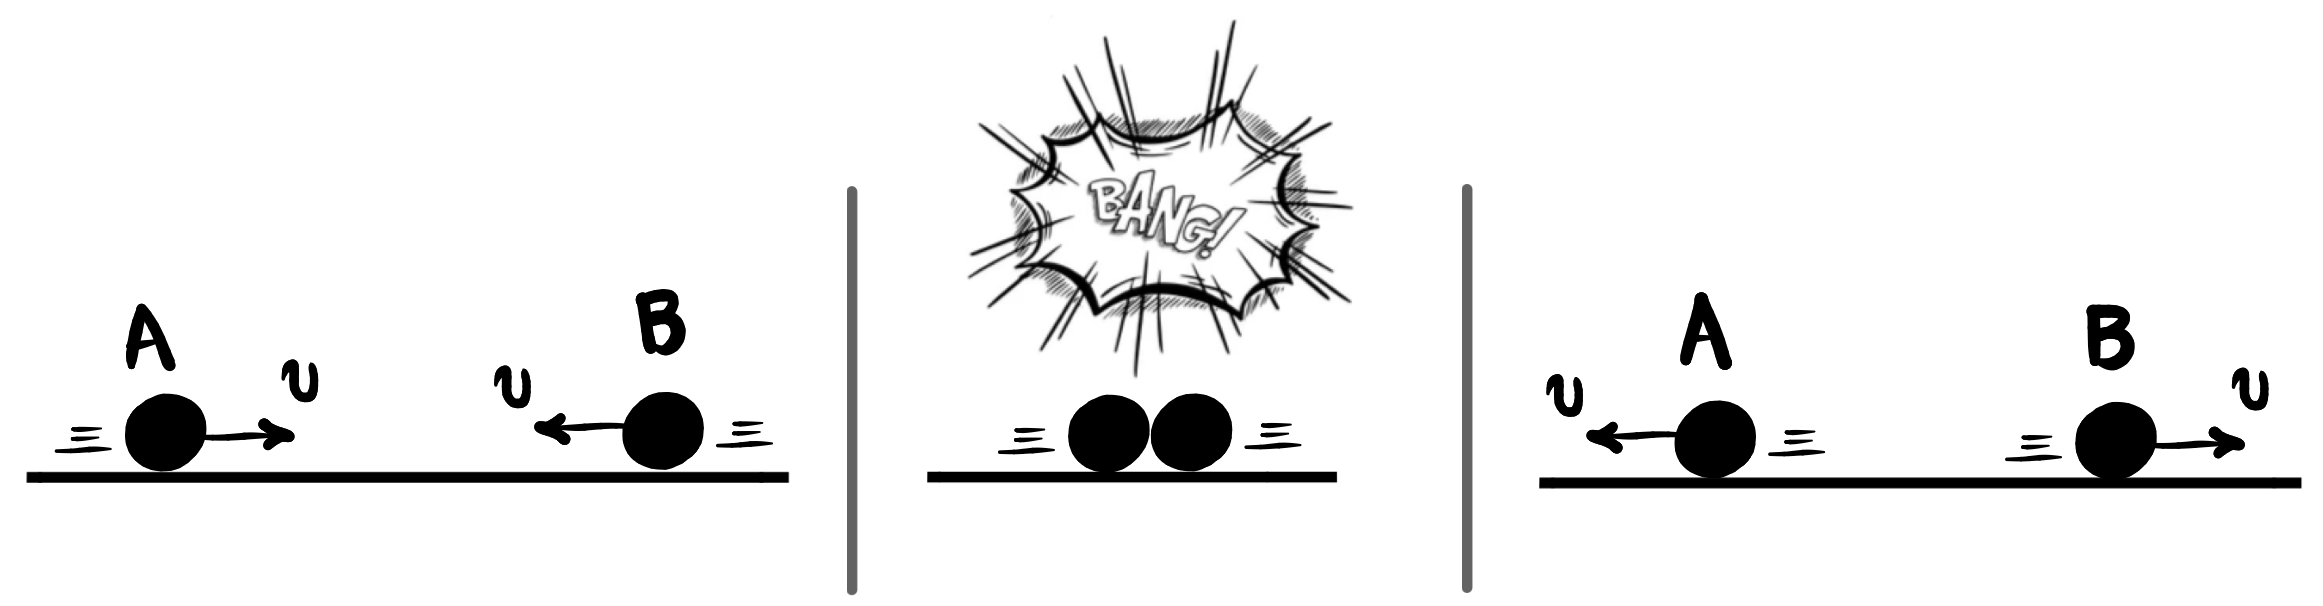
\includegraphics[width=0.8\linewidth]{imagensdinamicanewton/thirdlawnewton.png}};
  \end{scope}
\end{tikzpicture}
\captionof{figure}{Experimento de duas bolas, idênticas e de mesma velocidade, colidindo.}
\label{fig_dinamicanewton_thirdlawmomento}
} 
\vspace{0.3cm}

Ao fazer tal experimento, verifica-se que, após a colisão, as bolinhas mantêm o mesmo valor de velocidade, porém invertem o sentido do seu movimento. Ora, se houve variação do movimento (velocidade) então certamente houve aceleração. Mas a Segunda Lei de Newton diz que, para que haja aceleração, deve haver força resultante. Assim, a bolinha que inicialmente se movia para a direita deve ter sentido, durante a colisão uma força para a esquerda, de modo a variar seu movimento e inverter o sentido da sua velocidade. Já a bolinha que se movia para a esquerda deve ter sentido uma força para a direita, capaz de gerar uma aceleração e variar sua velocidade, de modo a inverter o sentido do seu movimento.

Dito isso, vemos que, durante este choque ideal, tudo indica que enquanto a bolinha $A$ bate na bolinha $B$, a bolinha $B$ também bate na bolinha $A.$ Ou seja, durante o choque, a bolinha $A$ faz uma força $F_{AB}$ na bolinha $B$, para a direita; porém a bolinha $B$ faz uma força -- no sentido contrário, para a esquerda -- $F_{BA}$ na bolinha $A.$

Ora, sendo as bolinhas idênticas (mesma massa) e tendo as duas sofrido exatamente a mesma variação de movimento (aceleração), as forças necessárias para que isso seja feito devem ser as mesmas, ou seja:

$$ F_{AB} = F_{BA},$$

\noindent o que, em palavras, quer dizer que a força com que a bolinha $A$ bate em $B$ tem exatamente o mesmo valor da força com que a bolinha $B$ bate em $A$.

Alguns estudantes costumam ter a curiosidade de saber qual é a ação e qual é a reação, mas isso é irrelevante e nem faz muito sentido. Seria o mesmo que perguntar: \textit{o que ocorreu primeiro, a bolinha $B$ bater em $A$ ou a bolinha $A$ bater em $B?$} Perceba que a pergunta não faz sentido porque as duas coisas ocorrem ao mesmo tempo: a colisão é um fenômeno único, e no mesmo instante em que $A$ faz a força $F_{AB}$ em $B,$ a bolinha $B$ faz a força $F_{BA}$ em $A.$ Ou seja, tanto faz quem é a ação e quem é a reação -- essa realmente é uma classificação que não tem importância alguma. O que importa é sempre o par ação-reação e o fato de que todas as forças sempre virão aos pares. Recapitulando, perceba que:

\begin{enumerate}
    \item [(i)] As forças $F_{AB}$ e $F_{BA}$ são de mesma natureza: forças de contato. Tais forças constituem um par ação-reação e, como neste caso, tal par sempre será constituído de forças de mesma natureza. Se a ação $F_{AB}$ for de natureza gravitacional, a reação $F_{BA}$ também será gravitacional. Se a ação for elétrica, a reação será também força elétrica, e por aí vai.
    
    \item [(ii)] As forças $F_{AB}$ e $F_{BA}$ atuam na mesma direção, possuem o mesmo valor porém sentidos contrários: a força $F_{AB}$ que $A$ faz em $B$ atua para a direita, enquanto a força $F_{BA}$ que $B$ faz em $A$ atua para a esquerda. Isso é exatamente o que está contido na relação vetorial da Equação \eqref{eq_newton_terceiraleinewton}.

    \item [(iii)] As forças $F_{AB}$ e $F_{BA}$ \textbf{atuam em corpos distintos: uma atua em $B$ e a outra em $A.$} Desse modo, um par ação-reação jamais irá se anular, justamente por atuarem em corpos distintos. 
    
    Não tem como a força peso que você está sentido agora se anular com a força peso que eu sinto, ainda que elas tenham o mesmo valor, mesma direção e sentidos contrários. Isso ocorre justamente pelo fato de que elas atuam em corpos distintos. A Figura \ref{fig_dinamicanewton_thirdlawcolision} deixa isso claro, onde analisamos as forças de interação durante a colisão. 
    
    É sempre útil desenhar os corpos separados espacialmente -- ainda que eles estejam ocupando o mesmo lugar do espaço -- a fim de conseguir visualizar com clareza qual é a força que atua em cada um deles.
    
\end{enumerate}


\vspace{0.3cm}
{
\centering
\begin{tikzpicture}
  \begin{scope}[blend mode=multiply]
    \node {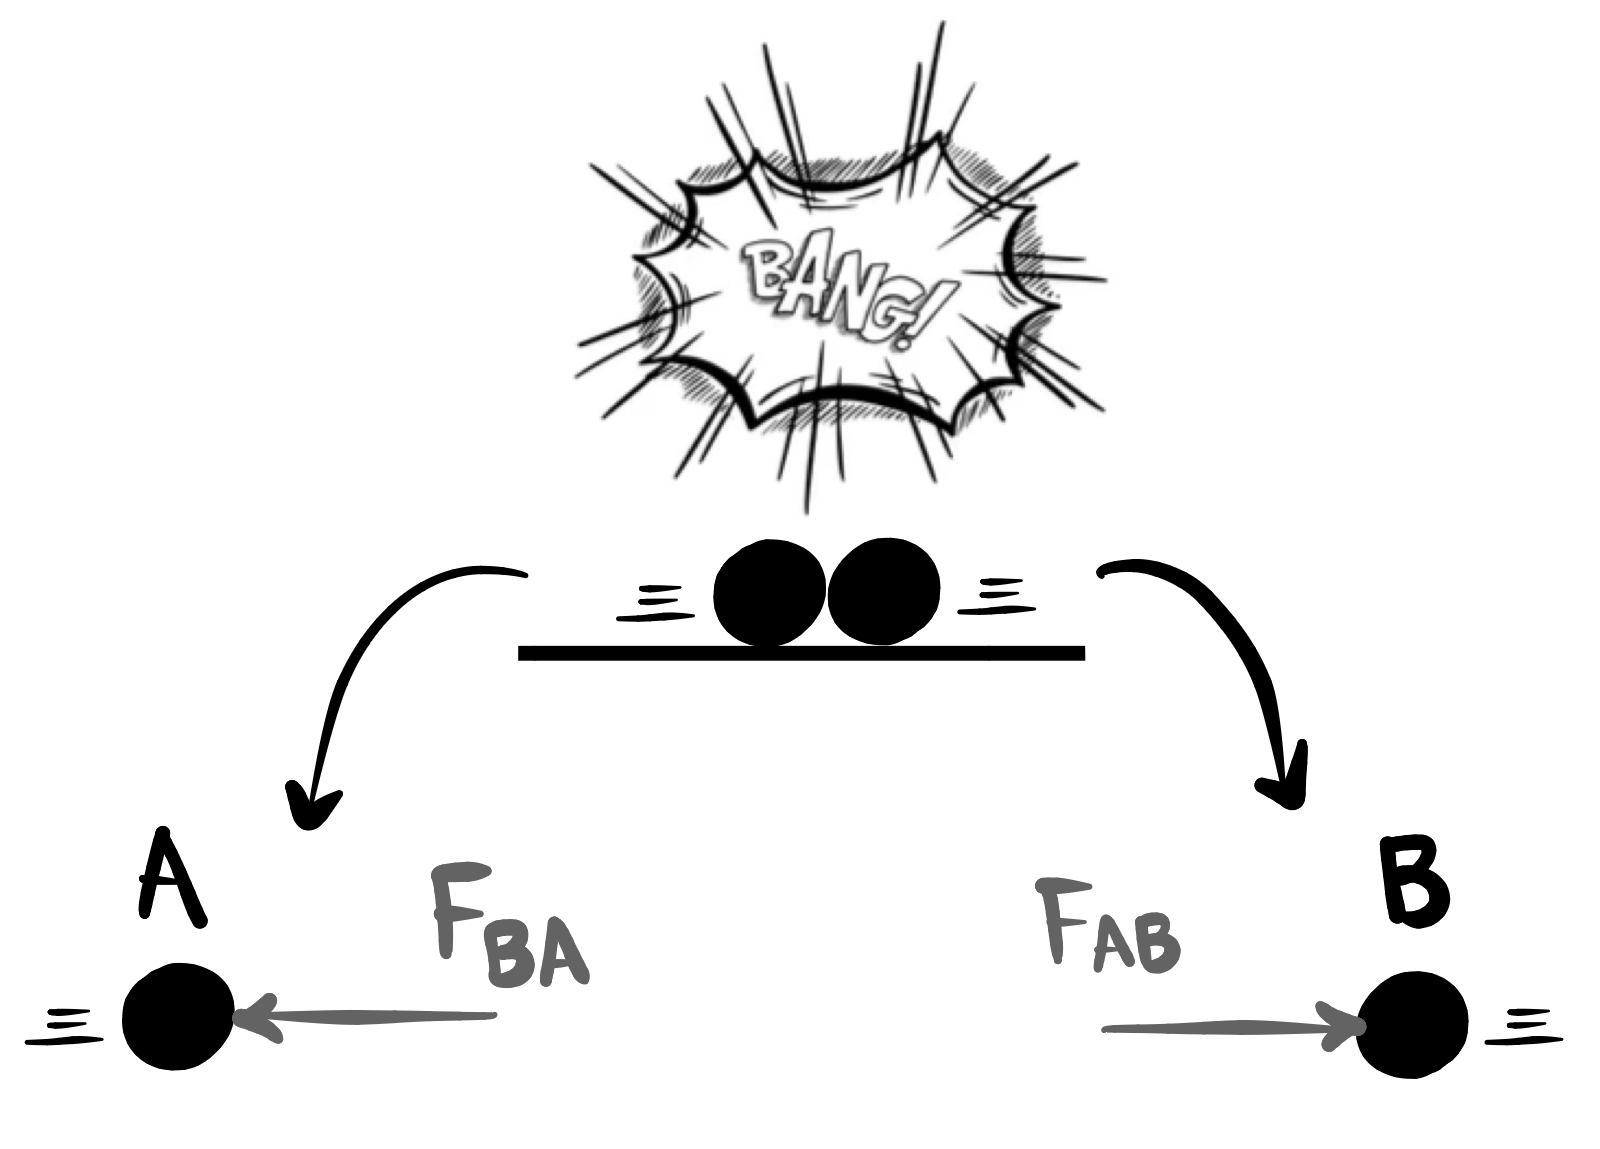
\includegraphics[width=0.4\linewidth]{imagensdinamicanewton/thirdlawcolision.png}};
  \end{scope}
\end{tikzpicture}
\captionof{figure}{Análise das forças de interação durante a colisão.}
\label{fig_dinamicanewton_thirdlawcolision}
} 
\vspace{0.3cm}




\secgfe{Onde é usada}

Como absolutamente todas as forças vem aos pares -- sem exceção -- a Terceira Lei de Newton acaba por aparecer em diversos contextos distintos e é usada para explicar uma enorme quantidade de fenômenos. 

Considere, por exemplo, a situação de uma simples caminhada: ao dar um passo, você está empurrando o chão para trás. Pela terceira lei de Newton, o chão reage e te empurra para frente, e é isso que possibilita que você ande. Essa força trocada entre os seus pés e o chão é chamada de força de atrito, e é por isso que em superfícies muito lisas -- com pouco atrito -- como em uma pista de gelo é bem difícil caminhar. A força de atrito e suas origens serão estudadas em detalhes em seções futuras.

Se você flexiona as pernas para dar um salto, ocorre algo parecido: você está empurrando o chão para baixo, que reage, empurrando você para cima: é por isso que você consegue saltar. \footnote{Sim, você está empurrando o planeta Terra para baixo ao dar um salto. Ocorre que a massa (inércia) dele é tão grande, mas tão grande, mas tão grande que esse seu empurrão sequer o tira do lugar.} A Figura \ref{fig_dinamicanewton_thirdlawatritoandar} mostra essas duas situações. 


\vspace{0.3cm}
{
\centering
\begin{tikzpicture}
  \begin{scope}[blend mode=multiply]
    \node {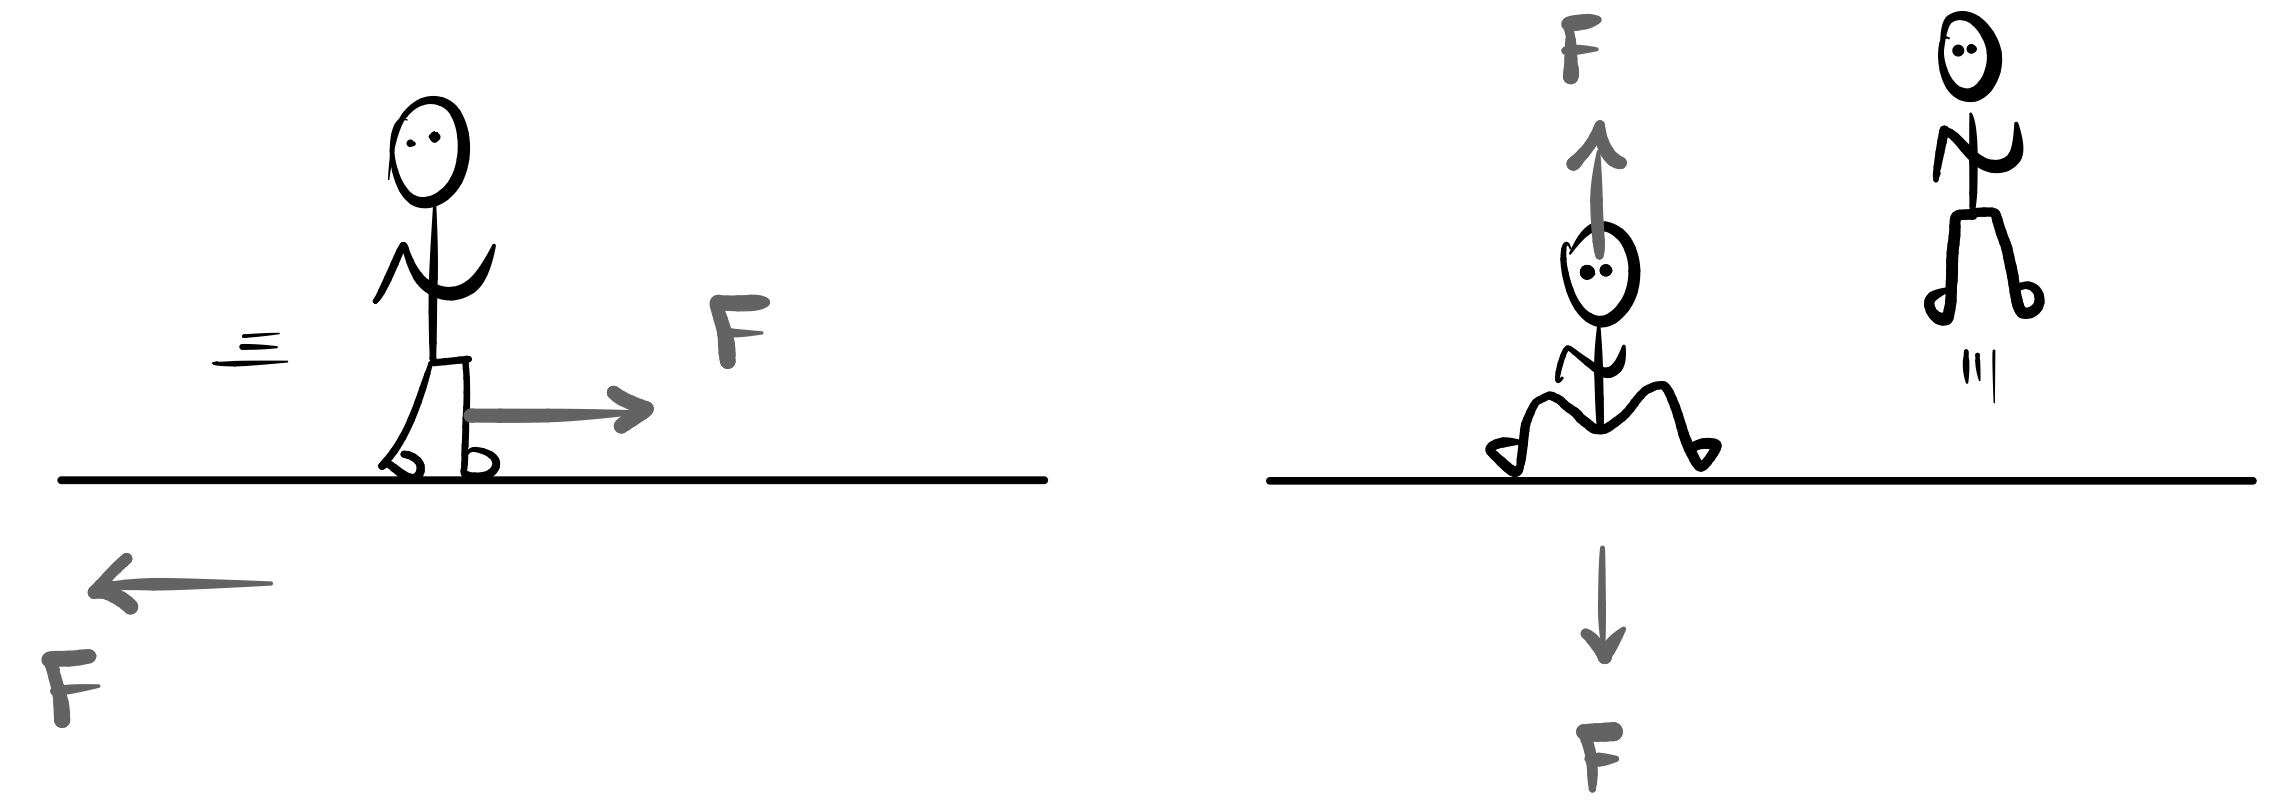
\includegraphics[width=0.55\linewidth]{imagensdinamicanewton/thirdlawexample.png}};
  \end{scope}
\end{tikzpicture}
\captionof{figure}{O par ação-reação das forças trocadas entre o menino e o chão durante uma caminhada e durante um salto, respectivamente.}
\label{fig_dinamicanewton_thirdlawatritoandar}
} 
\vspace{0.3cm}

A Terceira Lei de Newton também explica, por exemplo, como um foguete decola. No interior do foguete, o combustível é queimado, produzindo gases extremamente quentes. Esses gases são expelidos para trás com grande velocidade. Isso significa que o foguete exerce uma força sobre os gases, empurrando-os para trás. Pela Terceira Lei de Newton, os gases devem fazer uma força igual e contrária no foguete, empurrando-o para cima -- essa força propulsora para cima é a que faz o foguete decolar.



Um outro contexto importante que pode ser compreendido sob a luz da Terceira Lei de Newton é o da força que se manifesta em fios, chamada de tração. Observe a Figura \ref{fig_dinamicanewton_thirdlawatraction}, em que um menino puxa uma caixa por uma corda. O menino puxa a corda, na extremidade $1$, com uma força que chamamos de $T_1.$ Pela Terceira Lei, neste mesmo ponto, a corda puxa o menino com uma força igual e contrária. Isso está representado na segunda imagem de tal figura. 

Como o menino puxa a corda, este efeito se propaga e faz com que a corda, que está presa na caixa, puxe a caixa. Chamemos essa força de $T_2.$ Pela Terceira Lei, a caixa deve puxar a corda com uma força igual e contrária.

\vspace{0.3cm}
{
\centering
\begin{tikzpicture}
  \begin{scope}[blend mode=multiply]
    \node {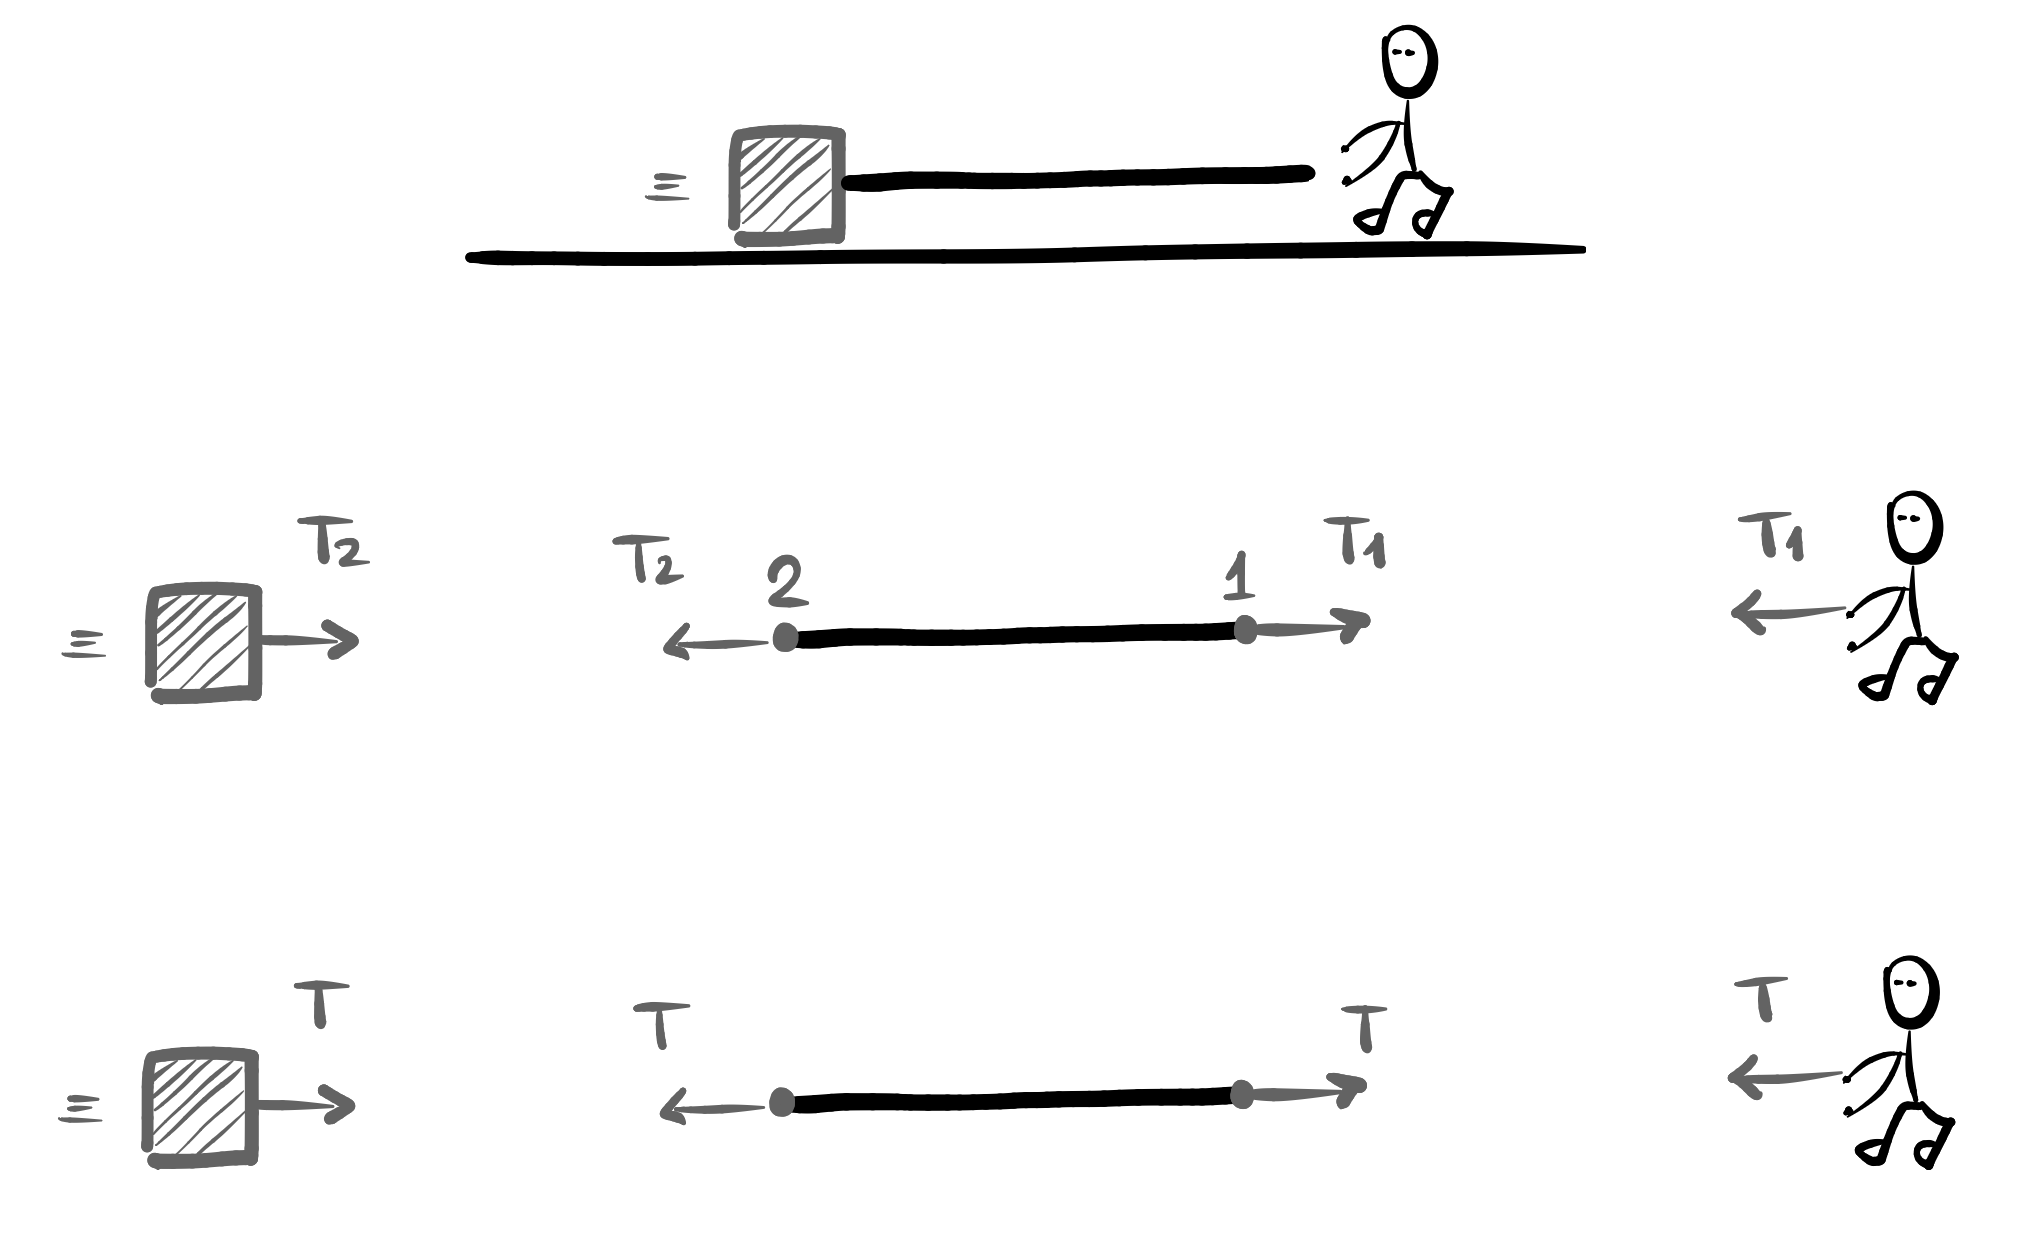
\includegraphics[width=0.8\linewidth]{imagensdinamicanewton/thirdlawtraction.png}};
  \end{scope}
\end{tikzpicture}
\captionof{figure}{A tração em um fio ideal.}
\label{fig_dinamicanewton_thirdlawatraction}
} 
\vspace{0.3cm}

Na quase totalidade dos problemas de Ensino Médio trabalharemos com fios ideais, que são aqueles de massa nula.\footnote{Como o próprio nome diz, é um fio ideal: trata-se de uma idealização, não existe nenhuma corda de massa zero. Isso se trata, na verdade, de uma aproximação: a massa da corda, em geral, será bem menor do que a massa das caixas que serão puxadas, por isso podemos considerar sua massa desprezível. Considere, por exemplo, uma corda de 100g, puxando uma caixa de 50 kg. A massa da corda é de apenas 0.2\% da massa da caixa, de modo que é uma aproximação razoável dizer que sua massa é praticamente zero, se comparada com a da caixa.} Sendo a sua massa nula, a Segunda Lei de Newton nos diz que 

$$ F_R = \cancelto{0}{m} a \implies F_R =0,$$

\noindent portanto, a força resultante em um fio ideal -- estando ele acelerado, parado ou em qualquer estado de movimento -- será sempre nula, ou seja, teremos $T_1=T_2,$ que poderemos chamar apenas de $T,$ para simplificar. Essa conclusão está ilustrada na terceira imagem da Figura \ref{fig_dinamicanewton_thirdlawatraction}: em um fio ideal a força feita em uma extremidade é propagada na íntegra ao longo do fio até a outra extremidade. Assim, no fio ideal, as forças nas suas extremidades -- as trações -- sempre terão o mesmo módulo.











A Terceira Lei de Newton também nos permite compreender uma força muito importante trocada entre dois corpos em contato: a força normal. Considere, por exemplo, uma caixa sob o chão, na superfície da Terra, como mostra a Figura \ref{fig_dinamicanewton_thirdlawnormal}. A caixa possui uma força peso $P$, que a puxa para baixo. Isso faz com que a caixa seja empurrada contra o chão, \textbf{comprimindo o chão}, por meio de uma força que chamamos de força normal $N.$ A caixa, portanto, empurra o chão para baixo, e, pela Terceira Lei, o chão reage e empurra a caixa para cima com uma força de mesmo módulo, direção, porém sentido contrário. \textbf{A força normal, portanto, é uma força de compressão entre duas superfícies em contato, e é sempre perpendicular a tal superfície de contato.}

\vspace{0.3cm}
{
\centering
\begin{tikzpicture}
  \begin{scope}[blend mode=multiply]
    \node {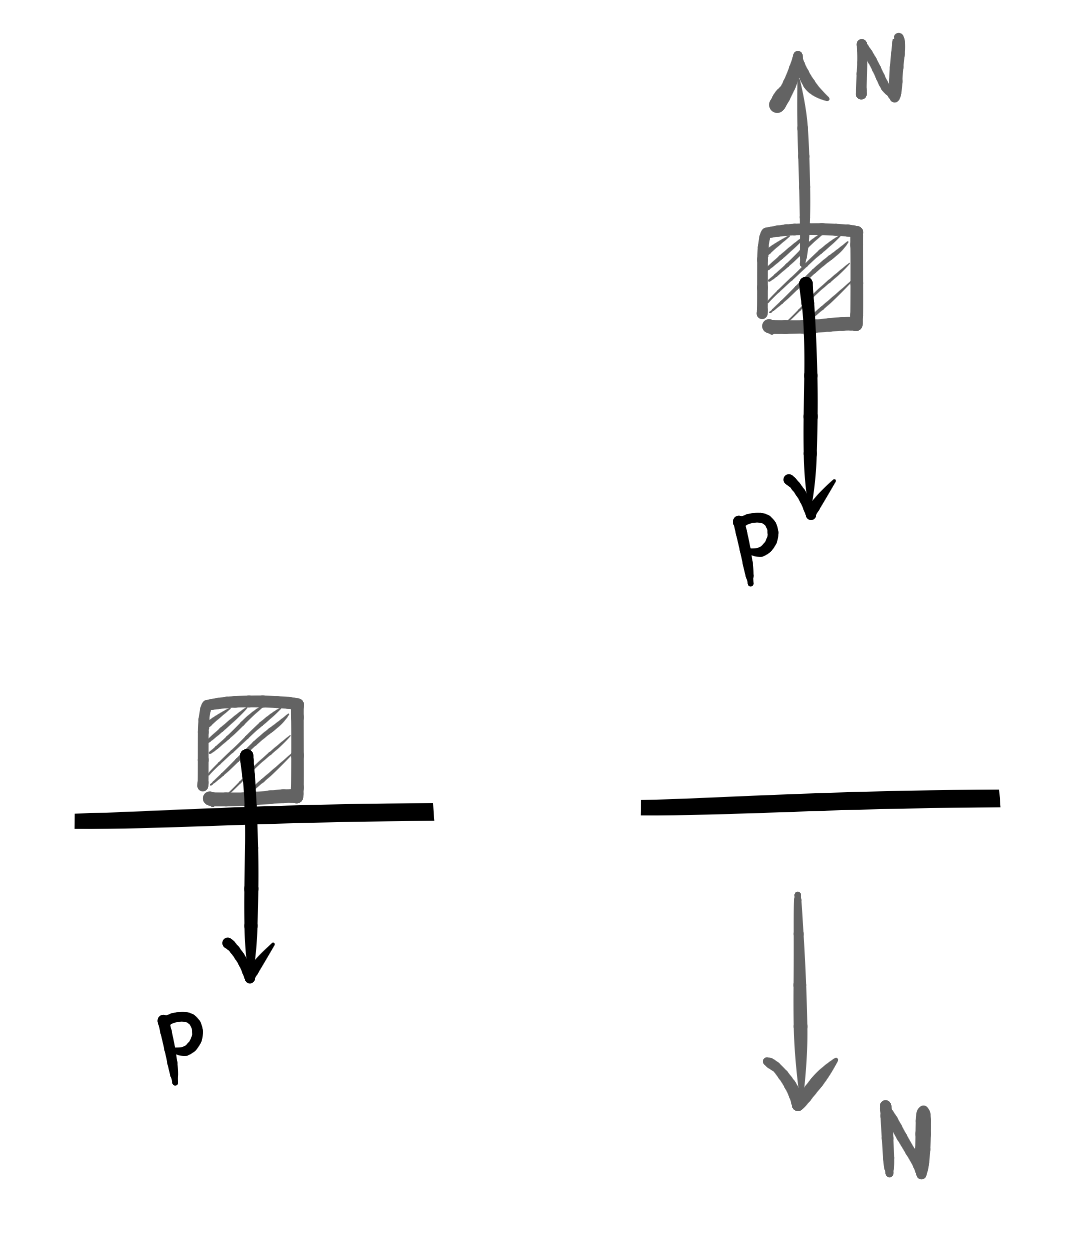
\includegraphics[width=0.3\linewidth]{imagensdinamicanewton/thirdlawnormal.png}};
  \end{scope}
\end{tikzpicture}
\captionof{figure}{A força normal é uma força de contato sempre perpendicular à superfície de contato entre os corpos.}
\label{fig_dinamicanewton_thirdlawnormal}
} 
\vspace{0.3cm}


Note algumas coisas neste contexto:

\begin{enumerate}
    \item [(i)] A força normal é uma força de contato, e recebe esse nome justamente pelo fato de que, em física, normal é sinônimo de perpendicular: a força normal é uma força de contato trocada entre dois corpos que estejam em contato, e tal força é sempre perpendicular à superfície de contato entre os corpos. A Figura \ref{fig_dinamicanewton_normalsempreperpendicular} ilustra algumas outras situações, destacando a força normal de contato entre o corpo e a superfície -- sendo tal força sempre perpendicular (normal) à superfície do corpo apoiado.  



\vspace{0.3cm}
{
\centering
\begin{tikzpicture}
  \begin{scope}[blend mode=multiply]
    \node {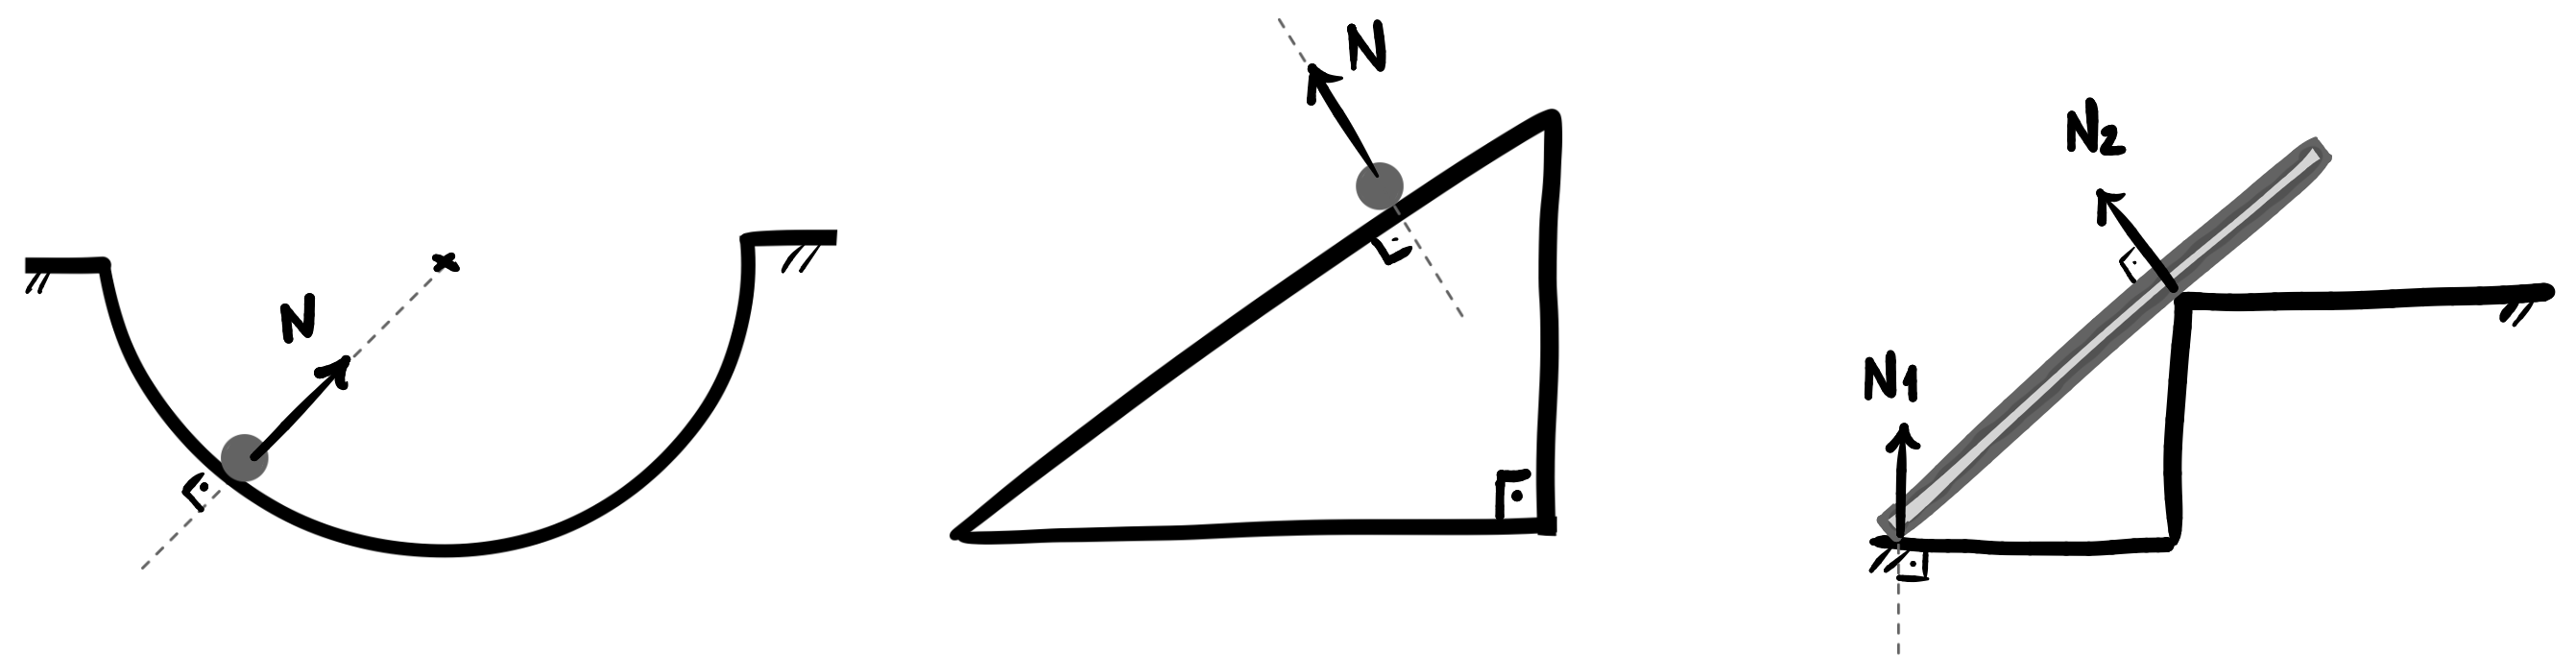
\includegraphics[width=0.95\linewidth]{imagensdinamicanewton/normalsempreperpendicular.png}};
  \end{scope}
\end{tikzpicture}
\captionof{figure}{A força normal é sempre perpendicular à superfície de contato entre os corpos.}
\label{fig_dinamicanewton_normalsempreperpendicular}
} 
\vspace{0.3cm}

Note que, na situação da última imagem da figura, a barra está apoiada em dois pontos -- no solo, horizontal, e na quina da parede vertical com a parede horizontal --, de modo que, tendo dois pontos de contato, existem duas forças normais distintas, representadas por $N_1$ e $N_2$. Note também, ainda nessa situação, que na quinta ficaria difícil de definir a direção perpendicular à superfície de apoio: neste caso, a normal $N_2$ é perpendicular à superfície da barra que está em contato com a quina. 
    
    
    \item [(ii)] Se a caixa estiver em repouso, teremos que $F_R=0,$ de modo que a força para cima deve anular a força para baixo, isto é, $N=P.$

    \item [(iii)] A normal e o peso \textbf{não constituem uma par ação-reação}. Elas, como visto, atuam no mesmo corpo: na caixa. Elas possuem, inclusive, naturezas distintas: a normal é uma força de contato enquanto o peso é uma força de interação gravitacional. O par ação-reação aqui é o par de forças normais trocadas entre o chão e a caixa: a reação da normal na caixa (força que o chão faz na caixa) é a normal no chão (força que a caixa faz no chão). Isso está destacado na segunda imagem da Figura \ref{fig_dinamicanewton_thirdlawnormal}.

    Um leitor mais auspicioso poderia perguntar: \textit{mas qual é a reação do peso na caixa?} Essa pergunta será respondida na subseção seguinte, mas já levanto a bola para o leitor chutá-la: se o peso é a força que a Terra (corpo A) faz na caixa (corpo B), a reação deve ser uma força de mesma natureza feita pelo corpo B no corpo A...conseguiu perceber de qual força se trata?

    
\end{enumerate}







\secgfe{Erros comuns}

A situação da Figura \ref{fig_dinamicanewton_thirdlawnormal} certamente já deve ter levado o leitor a cometer um dos erros mais comuns: não conseguir identificar com clareza quais são os pares ação-reação.

Note, naquele contexto, que a força peso é uma interação gravitacional entre a caixa (corpo $A$) e a Terra (corpo $B).$ Já a força normal é uma interação de contato entre a caixa (corpo $A)$ e o chão (corpo $C).$ Logo, veja que há três corpos em questão interagindo, de modo que, sendo as forças sempre em pares, precisamos analisar as interações dois corpos por vez. O erro muitas vezes cometido é sequer perceber quais são os corpos envolvidos nas interações -- e a representação da própria Figura \ref{fig_dinamicanewton_thirdlawnormal} já induz a este erro, por mostrar apenas dois dos três corpos que estão interagindo com as forças representadas na figura.

O mais correto, portanto, seria colocarmos todos os corpos no nosso esboço, como mostra a Figura \ref{fig_dinamicanewton_thirdlawclassictable}, em que consideramos a caixa apoiada em cima de uma mesa ao invés do chão, apenas para facilitar a representação. 

Perceba, pela primeira imagem, que ao representarmos as forças $P$ e $N$ na caixa, é fácil sermos induzidos ao erro, haja vista que cada uma dessas forças é exercida por um corpo diferente: o peso $P$ é exercido pela Terra, enquanto a força normal $N$ é exercida pela mesa. Assim, é bastante instrutivo separar os corpos dois a dois para analisar cada interação individualmente -- o que é feito nas próximas imagens dessa figura.

\vspace{0.3cm}
{
\centering
\begin{tikzpicture}
  \begin{scope}[blend mode=multiply]
    \node {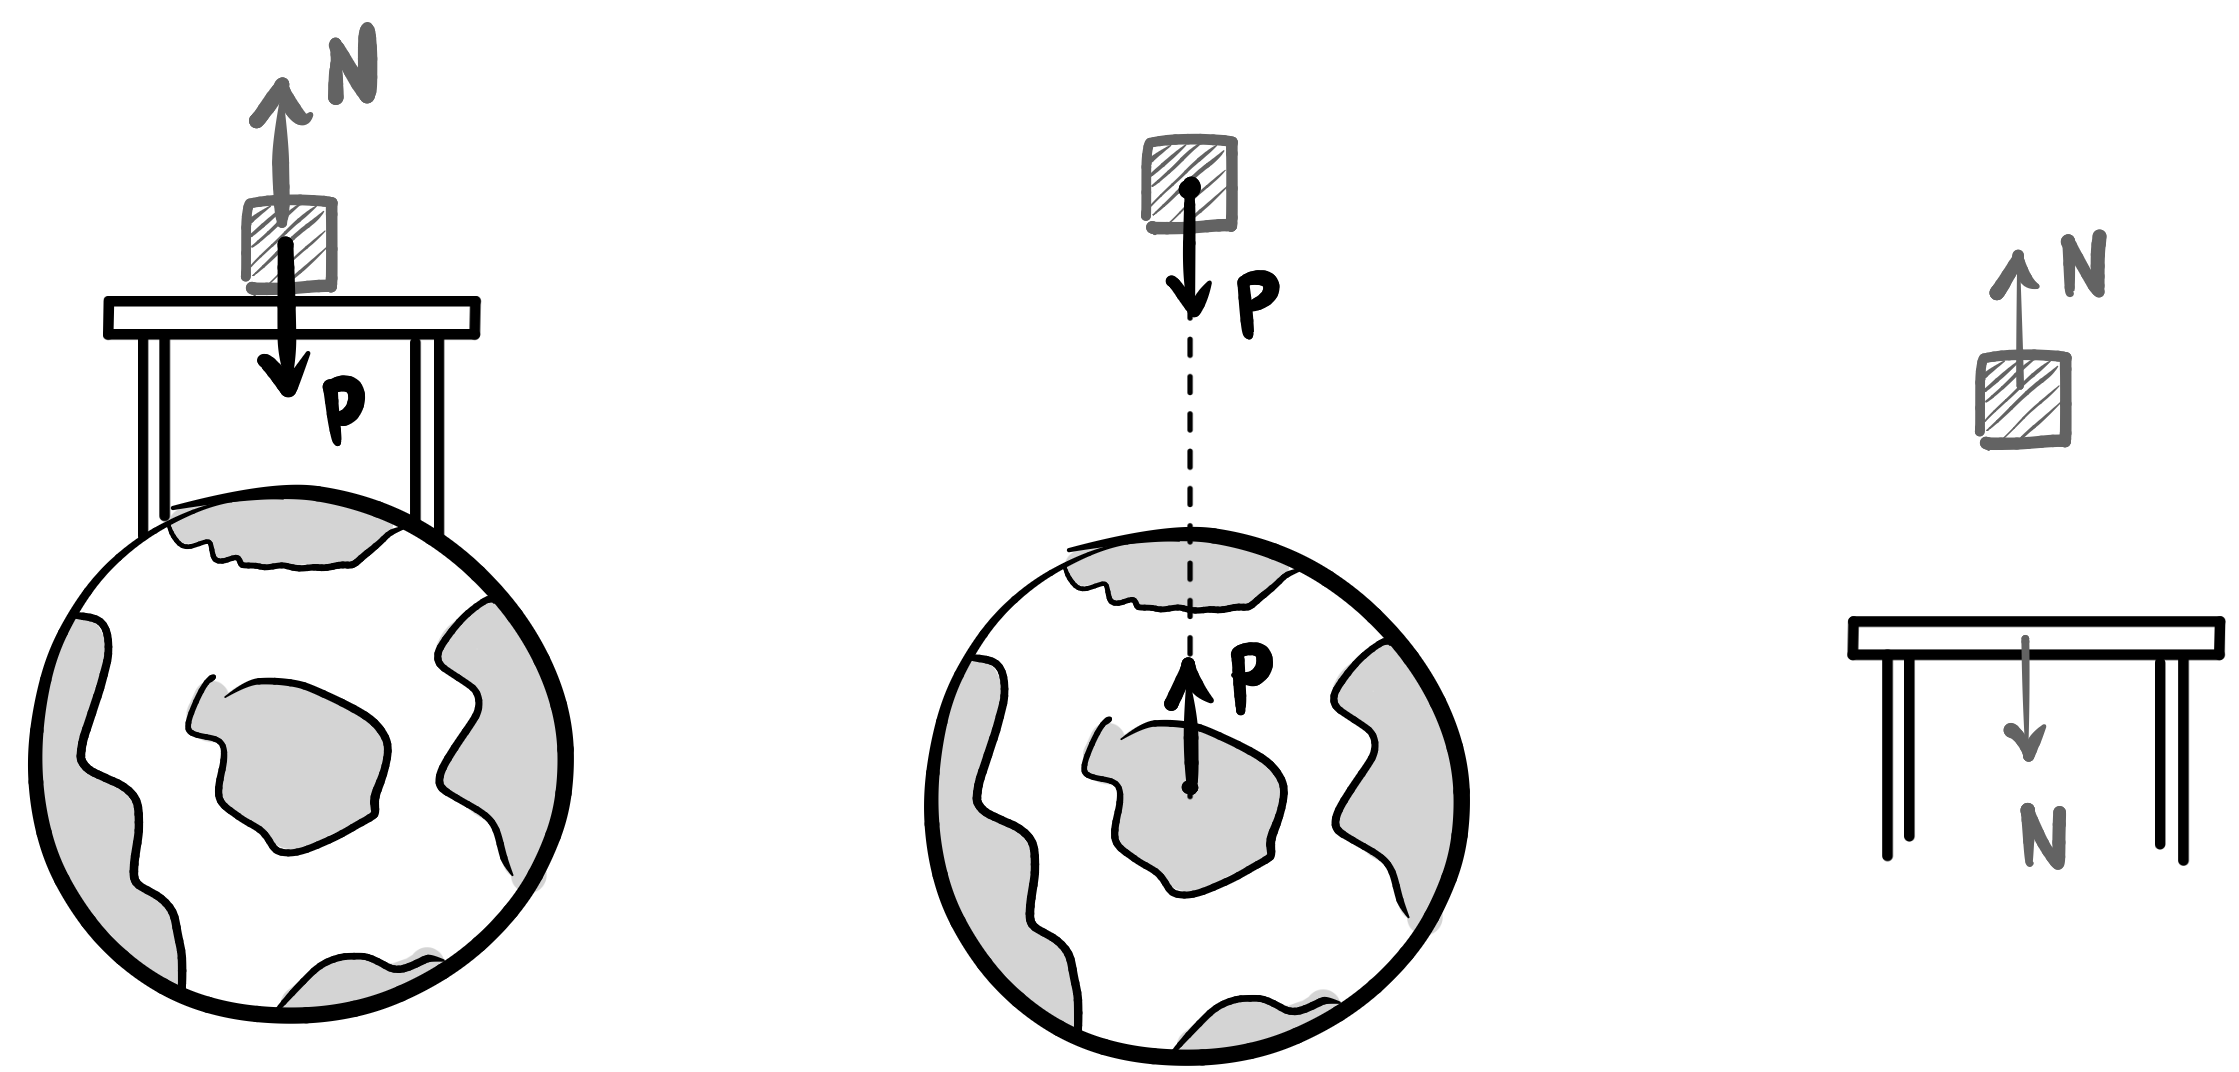
\includegraphics[width=0.6\linewidth]{imagensdinamicanewton/thirdlawclassictable.png}};
  \end{scope}
\end{tikzpicture}
\captionof{figure}{A Terceira Lei de Newton diz que as forças sempre vêm aos pares. Assim, é instrutivo sempre separar os corpos em pares para avaliar a respectiva intereção trocada entre eles.}
\label{fig_dinamicanewton_thirdlawclassictable}
} 
\vspace{0.3cm}


A primeira interação é entre a caixa e a Terra: se a Terra faz uma força $P$, gravitacional, na caixa, então a reação será a caixa fazendo uma força $P$, também gravitacional, de mesmo módulo, direção, porém sentido contrário, na Terra. Portanto, a reação do peso na caixa está no centro do planeta Terra, e é também uma força de natureza gravitacional.\footnote{Como a Terra tem uma massa (inércia) gigante, tal força é irrelevante e não altera o estado de movimento dela.}

Separando agora os outros dois corpos cuja interação nos interessa, temos a caixa e a mesa, na última imagem da Figura \ref{fig_dinamicanewton_thirdlawclassictable}. Por ter um peso que a puxa para baixo, a caixa empurra a mesa para baixo com uma força normal de contato $N.$ Desse modo, a mesa reage e faz uma força normal $N$ na caixa: essas duas forças são de mesma natureza, direção, módulo, porém sentidos contrários: constituem um par ação-reação.


Este é um ótimo exemplo e nos permite discutir os principais erros cometidos ao aplicar a Terceira Lei de Newton. Vamos recapitular brevemente cada um deles para que fique claro ao leitor:


\begin{enumerate}
    \item Achar que par ação-reação são forças que se cancelam. 
    
    O fato de que a normal e o peso se anulam na caixa, na situação da Figura \ref{fig_dinamicanewton_thirdlawclassictable}, já é razão suficiente para termos certeza de que essas duas forças não constituem um par ação e reação. 

    \item Não se dar conta de que o par ação-reação devem ser forças de mesma natureza. 

    Ainda na situação da Figura \ref{fig_dinamicanewton_thirdlawclassictable}: ao avaliar as forças na caixa, temos certeza de que a normal não é reação do peso porque a força peso é de natureza gravitacional, enquanto a normal é uma força de contato. São forças de naturezas distintas e jamais poderiam constituir um par ação-reação.

    \item Não separar adequadamente as forças nos diferentes corpos.

    Como feito em todas as análises, é extremamente instrutivo separar os corpos e representar, isoladamente, as forças em cada um deles. 
    
    Dado que o par ação-reação representa um par de forças trocadas por \textbf{dois corpos que interagem}, cada uma das forças desse par sempre irá atuar em um desses corpos, de modo que facilita muito desenhá-los separada e isoladamente para representar as forças em cada um deles. Foi o que fizemos na Figura \ref{fig_dinamicanewton_thirdlawclassictable}, analisando isoladamente as interações dos corpos de dois em dois: primeiro a Terra com a caixa, depois a caixa com a mesa.


\end{enumerate}




\secgfe{Observações}

Acredito que a observação mais relevante de todas a ser pontuada aqui -- correndo o risco de ser repetitivo -- é o conselho de sempre desenhar os corpos separados para avaliar a força que atua em cada um deles e não se embolar no par ação-reação. Foi isso que fizemos em todas as nossas análises dos exemplos que trouxemos -- incorpore este raciocínio e use-o.


\vspace{0.3cm}


\begin{exemplo}[Nível I]\label{exemplo_newton_terceiralei01}

Dois blocos, $A$ de massa $m_A = 6\,\text{kg}$ e $B$ de massa $m_B = 4\,\text{kg}$,
estão ligados por um fio ideal e repousam sobre uma superfície horizontal sem atrito.
Uma força horizontal $F = 30\,\text{N}$ é aplicada sobre o bloco $A$, conforme a
figura abaixo. 


\begin{center}
    \begin{tikzpicture}[
    >=Stealth,
    font=\small,
    bloco/.style={draw=black, thick, fill=none,
                  minimum width=1.5cm, minimum height=1.5cm}
  ]

  % ── blocos ──────────────────────────────────────────────────────
  \node[bloco] (A) at (0, 0.75)  {};
  \node[bloco] (B) at (3.2, 0.75) {};

  \node at (A.center) [yshift= 5pt]                  {$A$};
  \node at (A.center) [yshift=-7pt, font=\scriptsize] {$6\,\mathrm{kg}$};

  \node at (B.center) [yshift= 5pt]                  {$B$};
  \node at (B.center) [yshift=-7pt, font=\scriptsize] {$4\,\mathrm{kg}$};

  % ── fio ideal entre os blocos ────────────────────────────────────
  \draw[thick] (A.east) -- (B.west);

  % ── força aplicada em A ──────────────────────────────────────────
  \draw[->, line width=1.2pt]
    (-3, 0.75) -- (A.west)
    node[midway, above=2pt] {$F = 30\,\mathrm{N}$};

  % ── superfície ───────────────────────────────────────────────────
  \draw[thick] (-2.2, 0) -- (5, 0);
  \foreach \x in {-2.0,-1.5,-1.0,-0.5,0.0,0.5,1.0,1.5,2.0,2.5,3.0,3.5,4.0,4.5}
    \draw[thin] (\x, 0) -- (\x-0.3, -0.3);

\end{tikzpicture}
\end{center}






Determine:

\begin{enumerate}
    \item [a)] a aceleração do sistema;
    \item [b)] a tração $T$ no fio que conecta os dois blocos.
\end{enumerate}

\resolucao

\begin{enumerate}

    \item [a)] Como os blocos estão ligados por um fio inextensível, eles se movem
    juntos com a mesma aceleração. Podemos, portanto, tratar o sistema como um único
    corpo de massa total $m_A + m_B = 10\,\text{kg}$. Aplicando a Segunda Lei de
    Newton ao sistema:

    $$F_R = (m_A + m_B)\,a \implies 30 = 10\,a \implies \boxed{a = 3\,\text{m/s}^2.}$$

    \item [b)] Com a aceleração conhecida, isolamos agora apenas o bloco $B$. A única
    força horizontal que atua sobre ele é a tração $T$ do fio — e é exatamente isso
    que buscamos. Pela Segunda Lei de Newton aplicada ao bloco $B$:

    $$T = m_B \cdot a = 4 \cdot 3 = \boxed{12\,\text{N.}}$$

    Note que $T < F$: a força $F = 30\,\text{N}$ precisa acelerar o sistema inteiro
    ($m_A + m_B = 10\,\text{kg}$), enquanto a tração $T$ precisa acelerar apenas o
    bloco $B$ ($4\,\text{kg}$). É natural, portanto, que sejam diferentes.

\end{enumerate}


\end{exemplo}

\vspace{0.3cm}





\begin{exemplo}[Nível II]\label{exemplo_newton_terceiralei02}

Um menino empurra uma caixa de massa $m_A=8$kg, que, por sua vez, empurra uma segunda caixa de massa $m_B=4$kg. 

\vspace{0.3cm}
{
\centering
\begin{tikzpicture}
  \begin{scope}[blend mode=multiply]
    \node {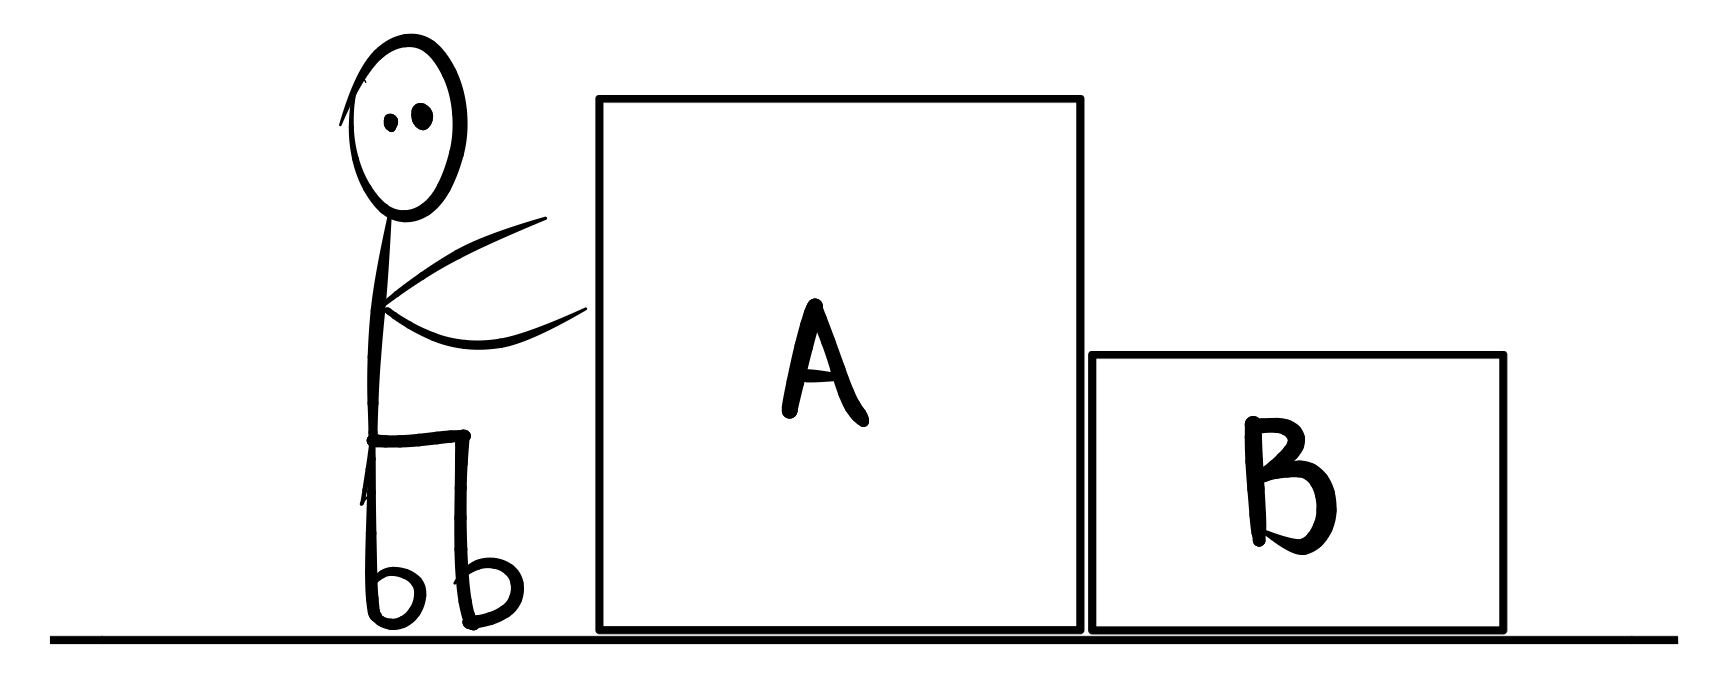
\includegraphics[width=0.4\linewidth]{imagensdinamicanewton/newtonforcasdecontatoexemplo1.png}};
  \end{scope}
\end{tikzpicture}
\captionof{figure}{}
\label{fig_dinamicanewton_newtonforcasdecontatoexemplo1}
} 
\vspace{0.3cm}

Se o menino faz uma força $F=24$N na caixa $A$, calcule:

\begin{enumerate}
    \item [a)] a aceleração do sistema.
    \item [b)] a força de contato entre as caixas.
\end{enumerate}

\resolucao

\begin{enumerate}
    \item [a)] Para computar a aceleração do sistema podemos proceder de duas formas:

    \begin{enumerate}
        \item [(i)] Considerar o sistema das caixas $(A+B)$ como um único corpo.

\vspace{0.3cm}
{
\centering
\begin{tikzpicture}
  \begin{scope}[blend mode=multiply]
    \node {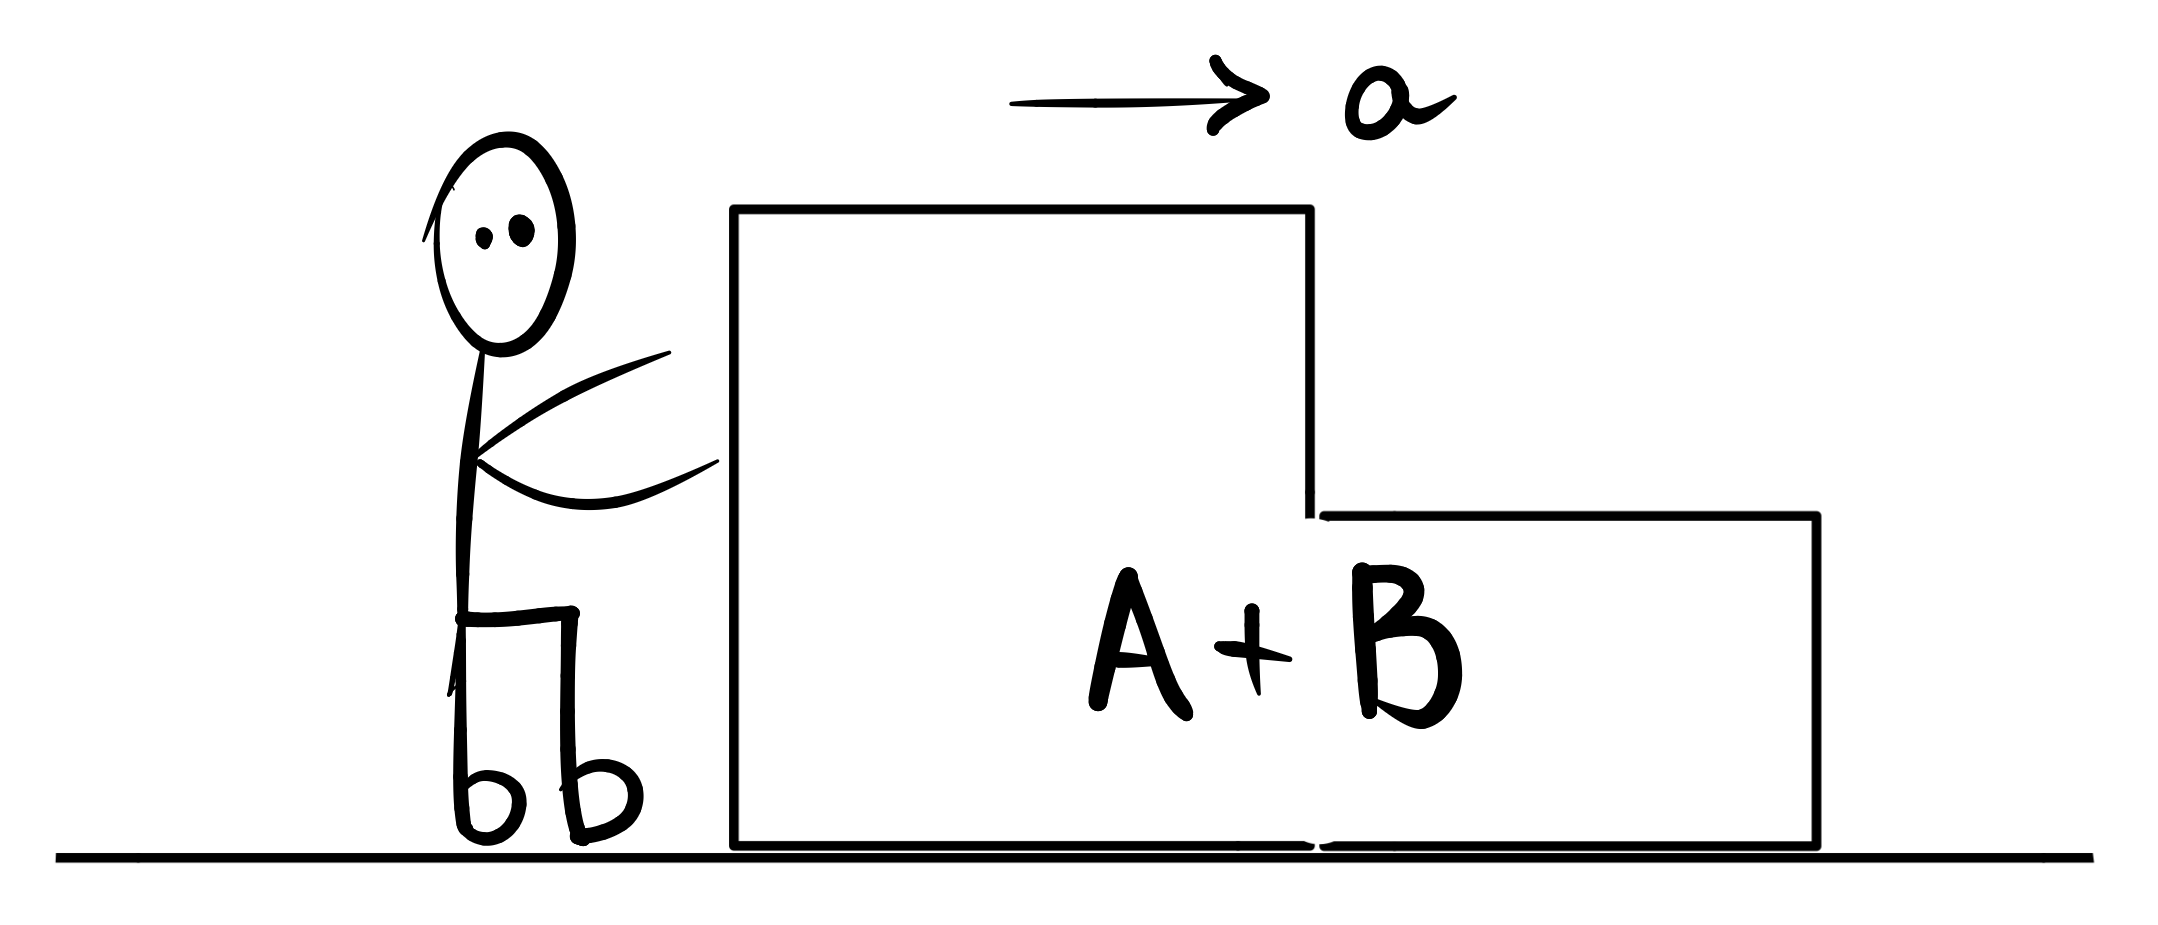
\includegraphics[width=0.4\linewidth]{imagensdinamicanewton/newtonforcasdecontatoexemplo3.png}};
  \end{scope}
\end{tikzpicture}
\captionof{figure}{}
\label{fig_dinamicanewton_newtonforcasdecontatoexemplo3}
} 
\vspace{0.3cm}

        
         Neste caso, o menino, com a força $F=24$N, deve acelerar $8+4=12$kg de massa. Assim, a Segunda Lei de Newton diz que

         $$ F_\text{R} = ma \implies 24 = (8+4)a \implies \boxed{a=2 \text{m/s}^2.}$$

         Note que, se o menino empurra a caixa $A$ de olhos vendados, ele jamais saberia que está tendo que empurrar uma única caixa de 12 kg, ou duas caixas de 6 kg, ou uma caixa de 8 kg e uma de 4 kg, como é o caso. O fato é que sua força $F$ deve ser capaz de acelerar 12 kg de massa, e é por isso que podemos usar este raciocínio de considerar os dois corpos $A$ e $B$ como se fossem um único corpo: porque os dois se moverão juntos, exatamente sob a mesma aceleração $a.$
         

         \item [(ii)] Considerar as caixas $A \text{ e }B$ como corpos separados.

         Neste caso, será preciso desenhar as forças (representaremos apenas as forças horizontais) que atuam individualmente em cada bloco. A Figura \ref{fig_dinamicanewton_newtonforcasdecontatoexemplo2} mostra isso: a caixa $A$ empurra a caixa $B$ com uma força de contato $F_C.$ Pela Terceira Lei de Newton, a caixa $B$ devolve uma força igual e contrária em $A.$

\vspace{0.3cm}
{
\centering
\begin{tikzpicture}
  \begin{scope}[blend mode=multiply]
    \node {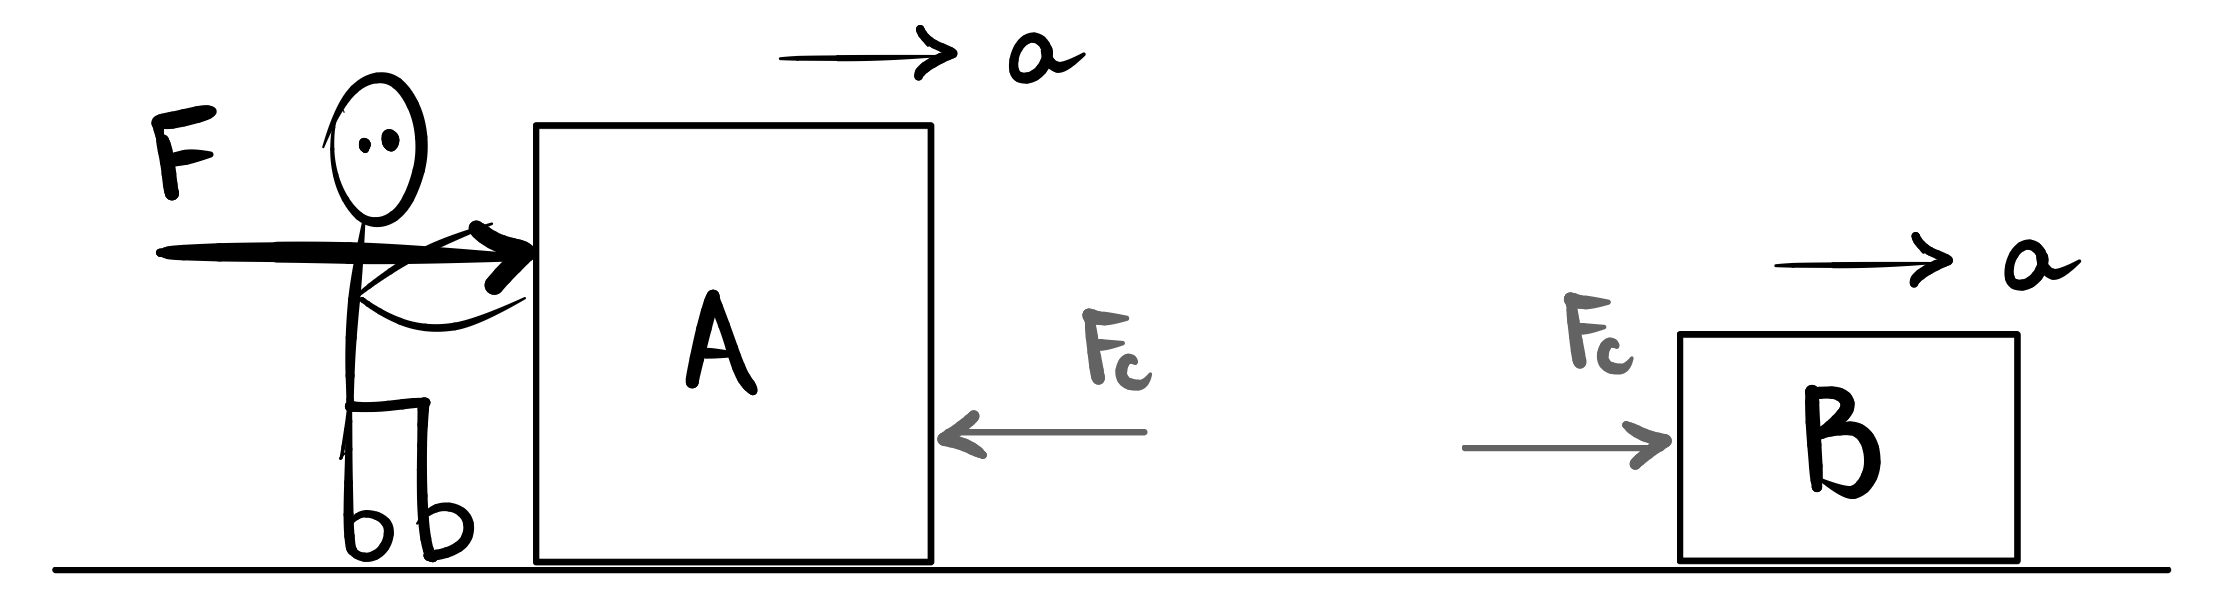
\includegraphics[width=0.65\linewidth]{imagensdinamicanewton/newtonforcasdecontatoexemplo2.png}};
  \end{scope}
\end{tikzpicture}
\captionof{figure}{}
\label{fig_dinamicanewton_newtonforcasdecontatoexemplo2}
} 
\vspace{0.3cm}


         Escrevendo a Segunda Lei de Newton para cada caixa individualmente, teremos, para as forças na horizontal:

         \begin{align}
             F_{\text{R}_A} &= m_A \cdot a_A \implies F - F_C = 8a \nonumber \\
            F_{\text{R}_B} &= m_B \cdot a_B \implies  F_C = 4a, \nonumber
         \end{align}

         \noindent e, somando as duas últimas equações, somos levados a

         $$ \begin{cases} 
           F - \cancel {F_C} = 8a \\
           \cancel {F_C} = 4a
         \end{cases} $$

\noindent ou seja,  $ F = 8a + 4 a = (8+4)a = 12 a.$ Como $F=24$ N, segue que $a= 2$ m/s$^2$, como esperado. Note que esse desenvolvimento prova porque podemos aplicar o raciocínio da solução anterior: ao somar as equações, a força de contato $F_C$ simplifica, restando apenas $F=(8+4)a = (m_A+m_B)a,$ ou seja, podemos olhar para o sistema das caixas como um único corpo -- neste caso, a força de contato desaparecerá, porque será uma força interna a este corpo -- e aplicar a Segunda Lei de Newton $F_R = M_T \cdot a,$ em que $M_T$ seria a massa total do sistema.

Note que isso só pode ser feito porque $a_1=a_2=a,$ isto é, porque os corpos se movem juntos, como se fossem um único corpo.
         
    \end{enumerate}
    
    
    
    \item [b)] Para computar a força de contato $F_C$ entre as caixas, a partir da segunda solução dada no item anterior, basta substituir o valor da aceleração em qualquer uma das equações para os corpos $A$ ou $B$. Fazendo para o corpo $B$, teremos:

    $$ F_C = 4a = 4 \cdot 2 = 8 \text{ N.}$$

    A título de verificação, façamos para a equação de movimento do corpo $A:$

    $$ F - F_C = 8a  \implies 24 - F_C = 8 \cdot 2 \implies F_C = 24 - 16 = 8 \text{ N } \checkmark $$
    
\end{enumerate}



\end{exemplo}



\vspace{0.3cm}


\begin{exemplo}[Nível III]\label{exemplo_newton_terceiralei03}

Tem-se \textit{n} blocos cuja massa cresce de 1 kg a cada bloco, ao se andar da direita para a esquerda, conforme mostra a Figura abaixo.

\vspace{0.3cm}
\begin{center}
\begin{tikzpicture}[
  block/.style = {draw, minimum width=1.4cm, minimum height=1.0cm,
                  font=\small, align=center},
  wire/.style  = {thick},
  >=stealth
]
  % Blocos da esquerda para a direita
  \node[block] (Bn) at (0,0)     {$n$\\kg};
  \node[block] (Bn1) at (2.2,0)  {$(n{-}1)$\\kg};
  \node        (dots) at (4.4,0) {\Large$\cdots$};
  \node[block] (B3) at (6.0,0)   {$3$\\kg};
  \node[block] (B2) at (8.2,0)   {$2$\\kg};
  \node[block] (B1) at (10.4,0)  {$1$\\kg};

  % Fios
  \draw[wire] (Bn.east)  -- (Bn1.west);
  \draw[wire] (Bn1.east) -- (dots.west);
  \draw[wire] (dots.east) -- (B3.west);
  \draw[wire] (B3.east)  -- (B2.west);
  \draw[wire] (B2.east)  -- (B1.west);

  % Força F
  \draw[->, very thick, black] (B1.east) -- ++(0.3,0)
        node[right, font=\normalsize, black] {$F$};
\end{tikzpicture}
\end{center}
\vspace{0.3cm}
% {
% \centering
% 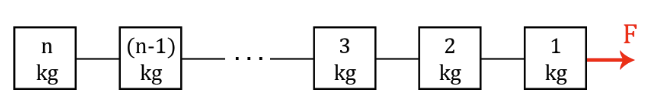
\includegraphics[width=0.6\linewidth]{imagensdinamicanewton/thirdlawexnivel3.png}
% \captionof{figure}{}
% \label{fig_dinamicanewton_thirdlawexnivel3}
% } 
% \vspace{0.3cm}


Os blocos estão conectados entre si por fios ideais e inextensíveis. Ao comunicar ao primeiro bloco -- a contar da direita -- uma força $F$, determine a expressão para a tração no \textit{p-ésimo} fio, em que o primeiro fio é aquele que conecta os blocos de massa 1 kg e 2 kg; o segundo fio é o que conecta os blocos de massa 2 kg e 3 kg, e assim por diante, ou seja, enumera-se os fios a contar da direita.

Discuta as condições de existência de tal expressão.

\resolucao

A chave deste problema é perceber que, uma vez obtida a aceleração do
sistema, a tensão em qualquer fio pode ser determinada isolando um
subsistema conveniente --- exatamente a estratégia que utilizamos no
exemplo anterior. Aqui, a novidade está em generalizar esse
procedimento para $n$ blocos e expressar o resultado em função de $p$.

\medskip
\noindent\textbf{Passo 1 — Aceleração do sistema.}

Tratando os $n$ blocos como um único sistema, todas as tensões internas
se cancelam. A única força horizontal externa é $F$. A massa total é:

\[
  M = 1 + 2 + 3 + \cdots + n = \frac{n(n+1)}{2}.
\]

Pela Segunda Lei:

\[
  a = \frac{F}{M} = \frac{2F}{n(n+1)},
\]

\noindent e todos os blocos do sistema se movem exatamente com essa mesma aceleração. Assim, ao aplicar a Segunda Lei para cada bloco (ou para um conjunto qualquer de blocos) já sabemos qual será a sua aceleração.

\noindent\textbf{Passo 2 — Tensão no $p$-ésimo fio.}

O $p$-ésimo fio (contando da direita) conecta o bloco de $p$\,kg ao
bloco de $(p+1)$\,kg. Para encontrar a tensão $T_p$, isolamos o
subsistema à \emph{esquerda} desse fio: os blocos de massas
$(p+1), (p+2), \ldots, n$\,kg. A única força horizontal sobre esse
subsistema é $T_p$, que o puxa para a direita.

A massa desse subsistema é:

\[
  M_{\text{esq}} = (p+1) + (p+2) + \cdots + n
  = \frac{n(n+1)}{2} - \frac{p(p+1)}{2}
  = \frac{(n-p)(n+p+1)}{2}.
\]

Aplicando a Segunda Lei ao subsistema:

\[
  T_p = M_{\text{esq}}\cdot a
      = \frac{(n-p)(n+p+1)}{2} \cdot \frac{2F}{n(n+1)},
\]

\[
  \boxed{T_p = \frac{(n-p)(n+p+1)}{n(n+1)}\,F.}
\]

\noindent\textbf{Verificação qualitativa.} Para $p = n-1$ (o fio mais
à esquerda, que puxa apenas o bloco de $n$\,kg):

\[
  T_{n-1} = \frac{1 \cdot (2n)}{n(n+1)}\,F = \frac{2F}{n+1}.
\]

Para $p = 1$ (o fio mais à direita, que arrasta todos os demais blocos):

\[
  T_1 = \frac{(n-1)(n+2)}{n(n+1)}\,F.
\]

Em ambos os casos, $T_p < F$, como deve ser: nenhum fio pode exercer
uma força maior do que a força externa que move o sistema inteiro.

\medskip
\noindent\textbf{Condições de existência da expressão.}

A expressão para $T_p$ existe e tem significado físico sob as seguintes
condições:

\begin{itemize}
  \item $n \geq 2$: são necessários pelo menos dois blocos para que
  haja algum fio;
  \item $p \in \{1, 2, \ldots, n-1\}$: $p$ deve ser inteiro positivo
  e não pode superar $n-1$, pois há exatamente $n-1$ fios no sistema;
  \item $F > 0$: a força deve ser não nula para que o sistema acelere e
  os fios fiquem tensionados; se $F = 0$, o sistema está em repouso e todas
  as tensões são nulas.
\end{itemize}

\noindent Para $p = n$, não existe fio --- seria o ``fio à esquerda do
bloco mais à esquerda''. Para $p = 0$, a expressão forneceria $T_0 =
F$, o que corresponderia à tensão imediatamente à direita do bloco de
\SI{1}{kg} --- ou seja, a própria força aplicada. Isso é formalmente
consistente, mas não há fio nessa posição: é apenas a continuidade
algébrica da fórmula além de seu domínio físico.



\end{exemplo}






\begin{secnivel}[Aceleração no Plano Inclinado]{I}{Aceleração no Plano Inclinado}
  
  \eqLdois{dem}{eq_dinamicanewtoniana_gsintheta}{a= g \sin (\theta)}

\end{secnivel}





\secgfe{De onde vem}

A Equação \eqref{eq_dinamicanewtoniana_gsintheta} fornece qual é a aceleração $a$ de um corpo que se move, exclusivamente sob a ação da gravidade, escorregando ao longo de um plano inclinado de $\theta$ em relação à horizontal em uma região em que a gravidade vale $g.$ 

Vamos construir tal equação, passando pausada e calmamente por cada etapa da resolução de um problema qualquer no campo da Dinâmica. Considere a Figura \ref{fig_dinamicanewton_planoinclinado01}. Vamos tentar dividir em etapas o nosso raciocínio:

\begin{enumerate}
    \item [(i)] Começamos desenhando as forças que atuam no corpo que queremos estudar -- no caso, a caixa. A força em questão -- que fará ela escorregar plano abaixo -- é o peso.

\vspace{0.3cm}
{
\centering
\begin{tikzpicture}
  \begin{scope}[blend mode=multiply]
    \node {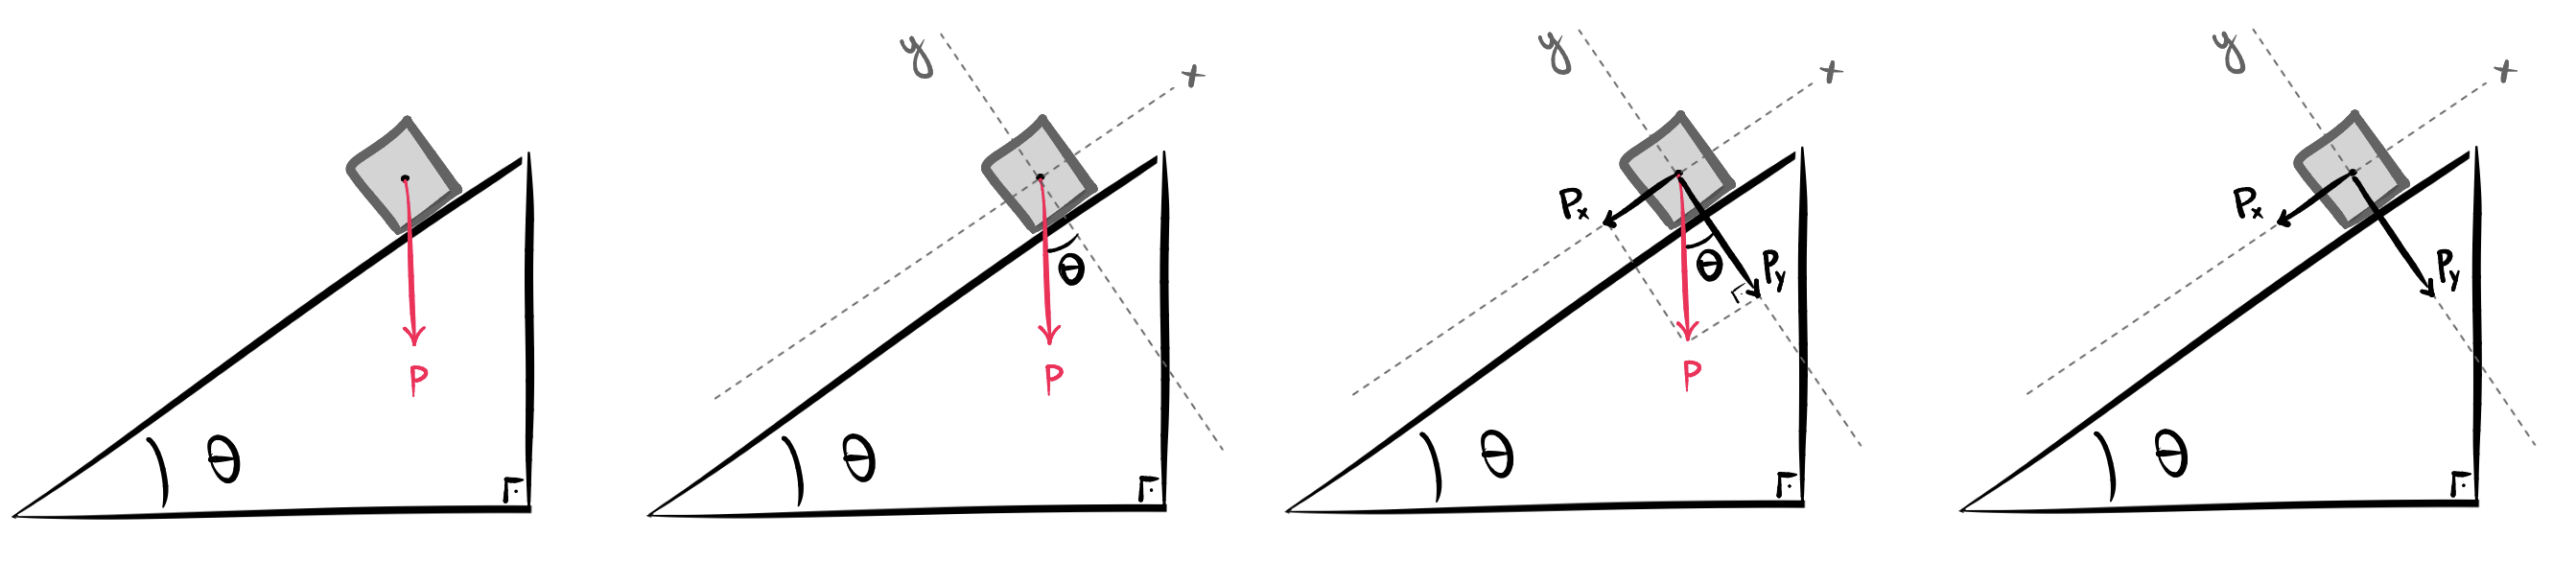
\includegraphics[width=1.0\linewidth]{imagensdinamicanewton/planoinclinado.png}};
  \end{scope}
\end{tikzpicture}
\captionof{figure}{Decomposição de forças no plano inclinado.}
\label{fig_dinamicanewton_planoinclinado01}
} 
\vspace{0.3cm}

\item [(ii)] O segundo passo é definir um sistema de eixos (sempre perpendiculares, como já explicamos ao estudar os vetores) nos quais iremos decompor as eventuais forças. \textbf{Um dos eixos sempre será aquele da direção na qual o movimento se dá, ou, caso prefira, este eixo será sempre paralelo ao vetor velocidade da partícula.} No caso, como ela irá escorregar plano abaixo, tal eixo será paralelo ao plano, representado na segunda imagem pelo eixo $x.$ O outro eixo, sendo perpendicular ao primeiro, será, portanto, perpendicular ao plano, representado pelo eixo $y.$

\item [(iii)] Definido o sistema de eixos, basta fazer a decomposição: isso aparece na terceira imagem da figura, e as componentes podem ser obtidas de forma direta usando as razões trigonométricas no triângulo retângulo dos vetores:

$$ \sin \theta = \dfrac{P_x}{P} \implies \boxed{P_x = P \sin \theta} \quad \text{ e } \quad \cos \theta = \dfrac{P_y}{P} \implies \boxed{P_y = P \cos \theta.} $$

Estamos, neste momento, interessados na resultante das forças na direção $x$: sendo essa a direção do movimento da caixa é nessa direção que aponta a velocidade da partícula, assim, a resultante das forças nessa direção será responsável pela aceleração tangencial:

$$ \sum F_x = ma_x \implies P \sin \theta = ma_x \implies \cancel{m}g \sin \theta = \cancel m a_x \implies \boxed{a_x = g \sin\theta,}$$

\noindent o que fornece a aceleração $a_x$ da caixa ao longo do plano.

\end{enumerate}

O passo-a-passo acima será basicamente a estrutura central de raciocínio para resolver qualquer problema de dinâmica. Algumas dúvidas, contudo, são naturais d surgirem no processo. A primeira delas, provavelmente, é sobre o ângulo $\theta$ do plano inclinado aparecer magicamente no triângulo dos vetores, entre a direção vertical e a direção perpendicular ao plano. 

\vspace{0.3cm}
{
\centering
\begin{tikzpicture}
  \begin{scope}[blend mode=multiply]
    \node {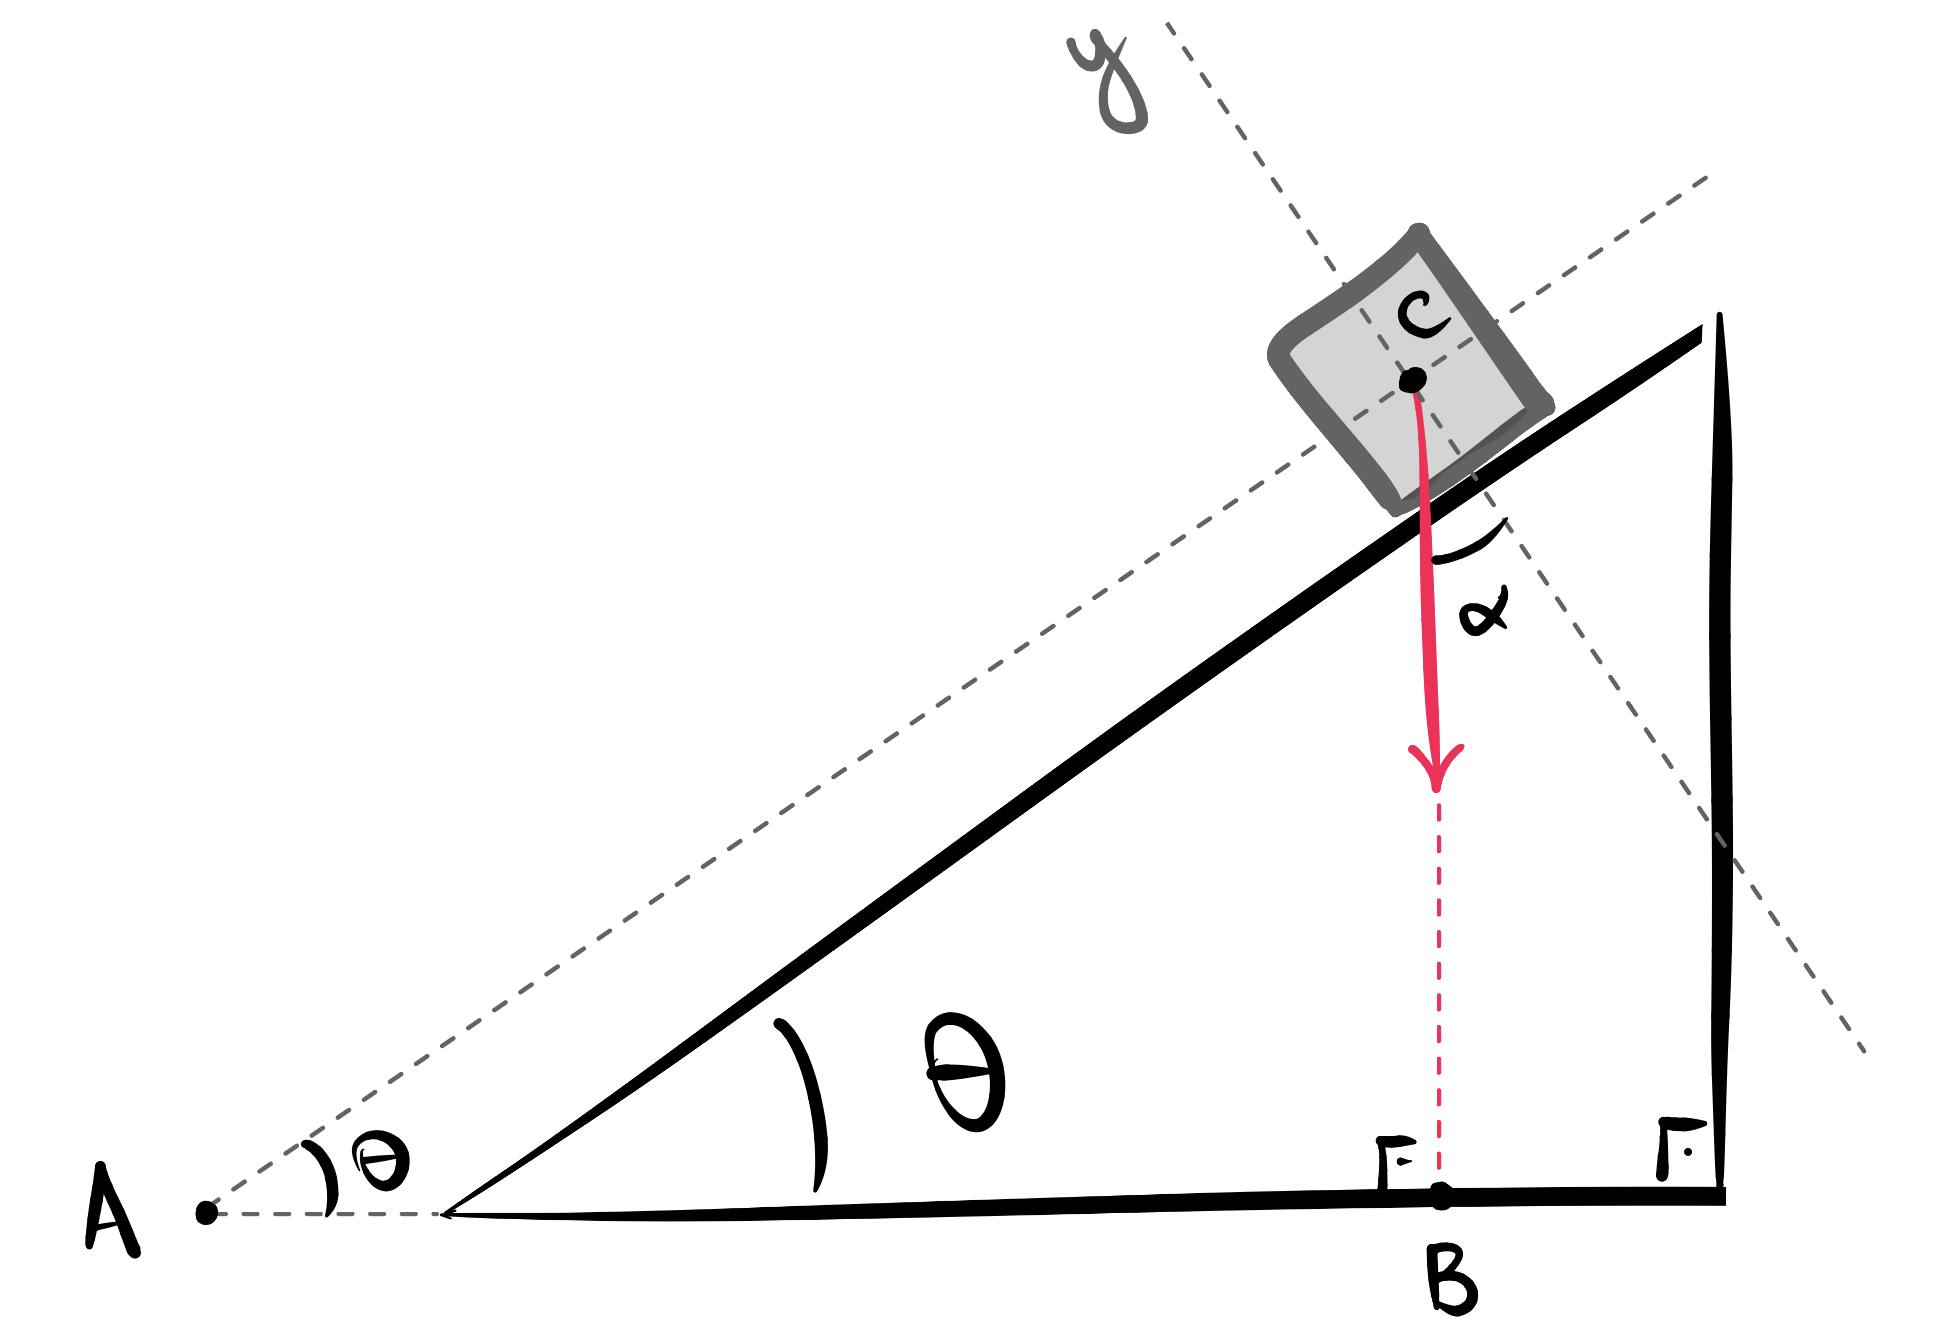
\includegraphics[width=0.35\linewidth]{imagensdinamicanewton/anguloplanoinclinado.png}};
  \end{scope}
\end{tikzpicture}
\captionof{figure}{O ângulo do plano inclinado no diagrama de vetores.}
\label{fig_dinamicanewton_planoinclinado02}
} 
\vspace{0.3cm}

A Figura \ref{fig_dinamicanewton_planoinclinado02} mostra um caminho possível para compreender como podemos encontrar tal ângulo: seja $C$ o ponto de aplicação da força peso, na caixa. Prolongue a direção da força peso até encontrar o solo, no ponto $B.$ Agora prolongue a direção $x,$ paralela ao plano inclinado, até encontrar o chão, no ponto $A.$ O ângulo $B\hat{A}C$ e o ângulo $\theta$ são correspondentes, de modo que suas medidas são iguais: $B\hat{A}C = \theta.$

Note, no triângulo $ABC$, que o ângulo $B\hat{C}A$ é complementar de $\theta$, e o ângulo $\alpha$ destacado é o complementar\footnote{Porque os eixos $x$ e $y$ são perpendiculares.} de $B\hat{C}A$, ou seja:

 $$ \alpha = \dfrac{\pi}{2} - \left( \dfrac{\pi}{2} - \theta \right) = \theta,$$



\noindent de modo que fica provado que o ângulo $\theta$ de inclinação do plano em relação à horizontal aparece entre a direção vertical e a direção perpendicular ao plano.


Uma segunda dúvida que poderia surgir é quanto à componente $P_y = P \cos \theta$ da força peso na direção perpendicular ao plano. Um primeiro comentário importante é o seguinte: as forças na direção perpendicular à direção $x$ são irrelevantes para o cálculo da aceleração na direção $x.$ Movimentos em direções perpendiculares são independentes, esse é um princípio enunciado por Galileu e que é crucial para a análise que fizemos: a aceleração na direção $x$ é determinada única e exclusivamente pela resultante das forças na direção $x$. Desse modo, podemos, como foi feito, isolar o problema e tratar separadamente apenas das componentes de força na direção do plano, uma vez que o que queremos computar é o valor da aceleração na direção do plano.

Dito isso, poderíamos fazer a análise das forças na direção $y$ -- apenas para enriquecer nossa discussão, uma vez que tais forças serão irrelevantes para o cálculo da aceleração na direção $x.$ Neste caso, vale separar os dois corpos em questão: a caixa e o plano inclinado. Por ter uma componente de peso $P_y$ puxando a caixa contra o plano, isso faz com que a caixa exerça uma força normal $N$ sob o plano inclinado, empurrando ele nessa direção. Pela Terceira Lei de Newton, o plano reage e faz uma força igual e contrária na caixa, como está representando na Figura \ref{fig_dinamicanewton_planoinclinado03}. 

\vspace{0.3cm}
{
\centering
\begin{tikzpicture}
  \begin{scope}[blend mode=multiply]
    \node {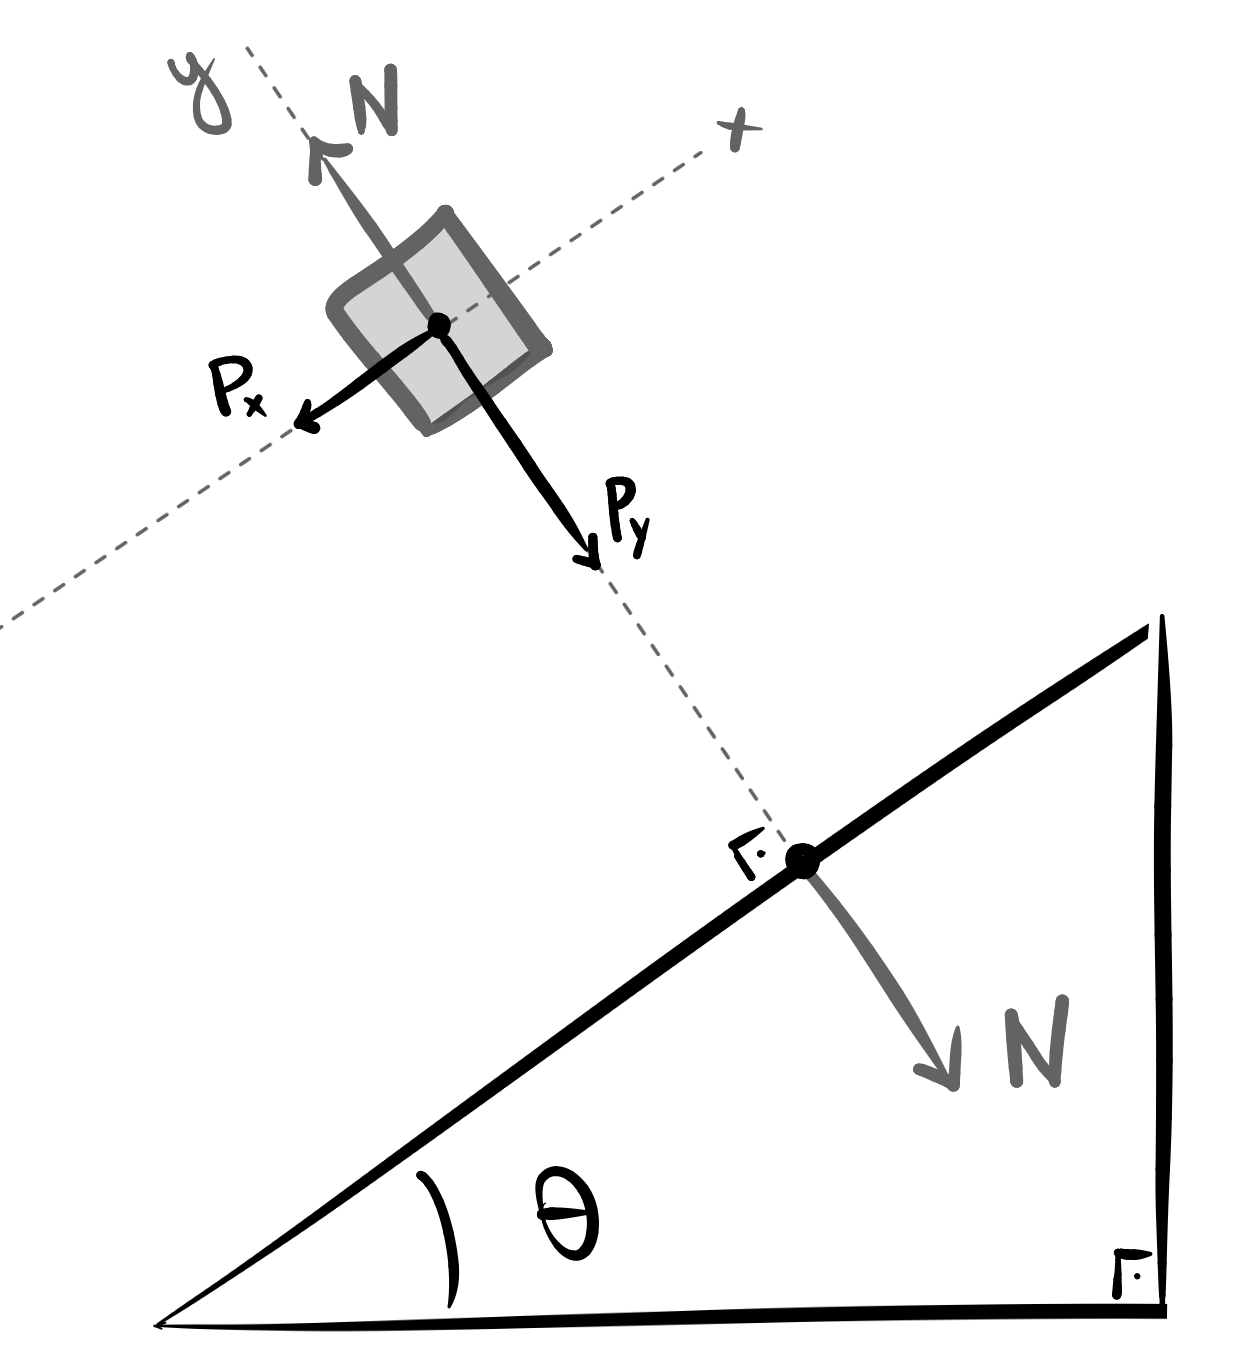
\includegraphics[width=0.3\linewidth]{imagensdinamicanewton/normalplanoinclinado.png}};
  \end{scope}
\end{tikzpicture}
\captionof{figure}{A resultante das forças na direção perpendicular ao plano.}
\label{fig_dinamicanewton_planoinclinado03}
} 
\vspace{0.3cm}

Para concluir a análise do problema, vemos que a caixa acelera -- e na verdade, só se move -- na direção $x.$ Sendo assim, a resultante das forças na direção $y$ deve ser nula, e concluímos que a componente $P_y$ do peso é anulada pela força normal que o plano faz na caixa:

$$ P_y = P \cos \theta = N.$$

A equação acima permitiria, sabendo a massa da caixa e o ângulo $\theta$ do plano inclinado, calcular o valor da força normal $N$ trocada entre o plano e a caixa. Como já pontuado, tal cálculo é irrelevante se o problema é computar a aceleração da caixa na direção $x$.





\secgfe{Onde é usada}

Essa é fácil e não hei de enrolá-lo, amigo leitor: essa equação é usada em problemas de plano inclinado. Contudo, para além disso, toda a discussão que fizemos e faremos aqui é bem mais ampla: envolve decomposição de vetores, escolha dos eixos mais adequados para fazê-lo, análise de casos particulares, etc. Todo esse ferramental, na verdade, se aplicará em praticamente qualquer problema sobre leis de Newton. 

Sendo assim, amigo leitor, não suponha que esta seção tenha nascido apenas para apresentá-lo à Equação \eqref{eq_dinamicanewtoniana_gsintheta}. A pobre equação serviu-nos, na verdade, de pretexto para conversarmos sobre princípios mais fundamentais na arte de analisar um problema de dinâmica.


% Sendo assim, caro leitor, não entenda essa seção como tendo o objetivo principal de apenas apresentá-lo à Equação \eqref{eq_dinamicanewtoniana_gsintheta}. Tal equação foi, na verdade, apenas uma cômoda desculpa para discutirmos princípios fundamentais da análise de um problema de dinâmica.

\secgfe{Erros comuns}

Eu diria — e digo com alguma experiência — que o erro mais comum é o estudante recorrer imediatamente à Equação \eqref{eq_dinamicanewtoniana_gsintheta}, como quem saca uma ferramenta da caixa sem sequer examinar a peça que tem diante de si.

Não me entenda mal: a equação pode, sim, ser usada diretamente. Aliás, esse é justamente o seu mérito. Uma boa equação condensa uma longa caminhada de raciocínios, poupando-nos de repeti-la a cada novo problema. É um atalho honesto, conquistado a duras penas pelo pensamento.

O perigo, porém, é sutil: quanto mais você se habitua a usar a fórmula pronta sem reconstruí-la por conta própria, menos exercita a musculatura do raciocínio — e pensamento, como qualquer músculo, enferruja quando não é usado.

Permita-me, então, um conselho que dou a você e que já dei a mim mesmo — e cumpri: use a forma direta da Equação \eqref{eq_dinamicanewtoniana_gsintheta} apenas depois de tê-la reconstruído, do zero, umas dez ou quinze vezes, como fizemos aqui. Pode parecer excesso de zelo, mas não é. Mesmo que o resultado já seja conhecido, o caminho ainda não o é — e é ele que forma o entendimento.

Os atalhos são úteis, mas há sempre o risco de nos fazer esquecer por onde passa a estrada principal. Convém, de quando em quando, voltar a percorrê-la.

% Eu diria que o erro mais comum é o estudante utilizar diretamente a Equação \eqref{eq_dinamicanewtoniana_gsintheta} sem se dar ao trabalho de construir todo o raciocínio que fizemos para chegar nela. Sim, é claro que ela pode ser usada diretamente e, de certo modo, este é o valor de uma equação: condensar toda uma caminhada de raciocínios para que eles não precisem ser empregados sempre e possamos, de modo prático, obter uma solução quase pronta para algum tipo de problema.

% Contudo, note o perigo: quanto mais você se exime de construir o racíocinio por si só e usa fórmulas prontas, menos você desenvolve e afia a sua capacidade de pensar. Sendo assim, eu lhe dou o conselho que eu daria para mim mesmo -- e foi exatamente o que fiz quando estudei tal equação pela primeira vez -- diante dessa situação: só use, de forma direta, a fórmula pronta da Equação \eqref{eq_dinamicanewtoniana_gsintheta} após ter construído-a, do zero, como fizemos, umas 10 ou 15 vezes. Isso será importante para desenvolver o seu entedimento e compreensão de tudo que fizemos -- mesmo que te leve a um resultado que você já conhece e pode usar de imediato. Muitas vezes os atalhos nos afastam do caminho original...é preciso tomar cuidado.



\secgfe{Observações}


É importante perceber que a Equação \eqref{eq_dinamicanewtoniana_gsintheta} vale para quaisquer valores de $\theta$, de modo que podemos também atestar sua validade avaliando o resultado que ela fornece para alguns ângulos cujo movimento seria trivial.

\vspace{0.3cm}
{
\centering
\begin{tikzpicture}
  \begin{scope}[blend mode=multiply]
    \node {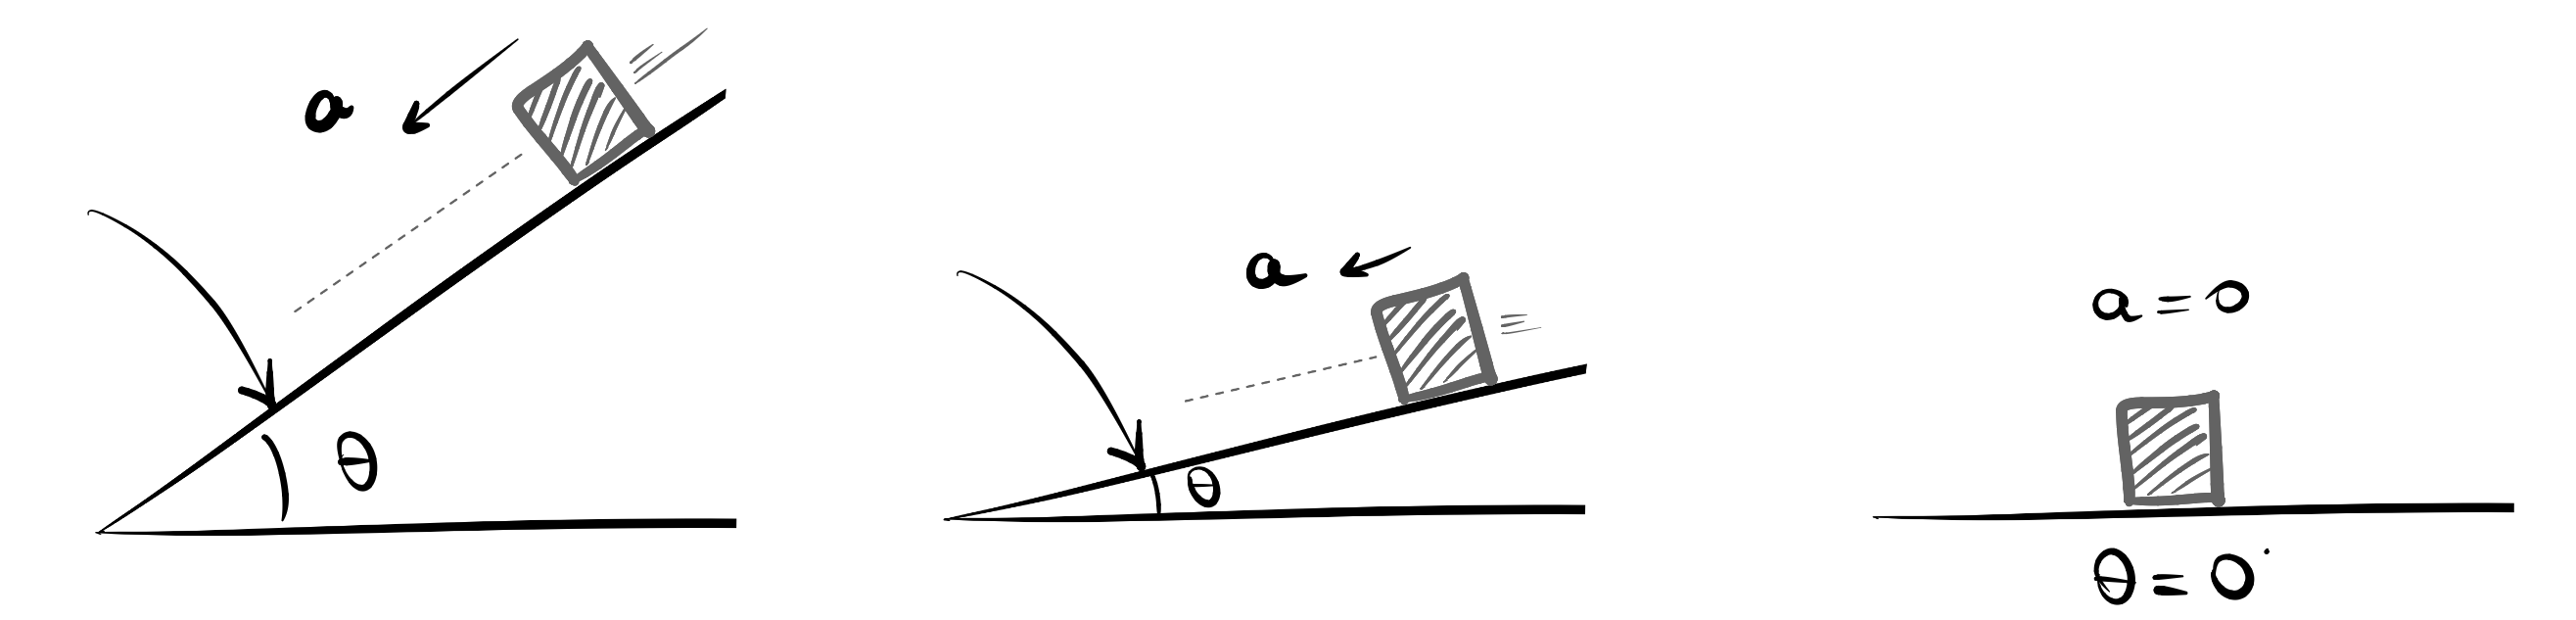
\includegraphics[width=0.8\linewidth]{imagensdinamicanewton/gsinthetacasoparticular1.png}};
  \end{scope}
\end{tikzpicture}
\captionof{figure}{Ao diminuir a inclinação do plano a aceleração da caixa deve diminuir, até zerar quando a inclinação do plano for nula.}
\label{fig_dinamicanewton_gsinthetacasoparticular1}
} 
\vspace{0.3cm}

Considere, por exemplo, a Figura \ref{fig_dinamicanewton_gsinthetacasoparticular1}. Nela, a cada nova etapa, o ângulo de inclinação do plano diminui. Isso faz com que a aceleração diminua e, no caso limite, quando deitarmos totalmente o plano e o ângulo for zero, o corpo estará em repouso: sua aceleração será nula. Ou seja, estamos dizendo que se $\theta =0,$ então devemos ter $a=0,$ uma vez que o corpo estará em um plano horizontal. Isso de fato ocorre, uma vez que $\sin 0 = 0,$ logo:

$$ a= g \sin 0 = 0.$$

\vspace{0.3cm}
{
\centering
\begin{tikzpicture}
  \begin{scope}[blend mode=multiply]
    \node {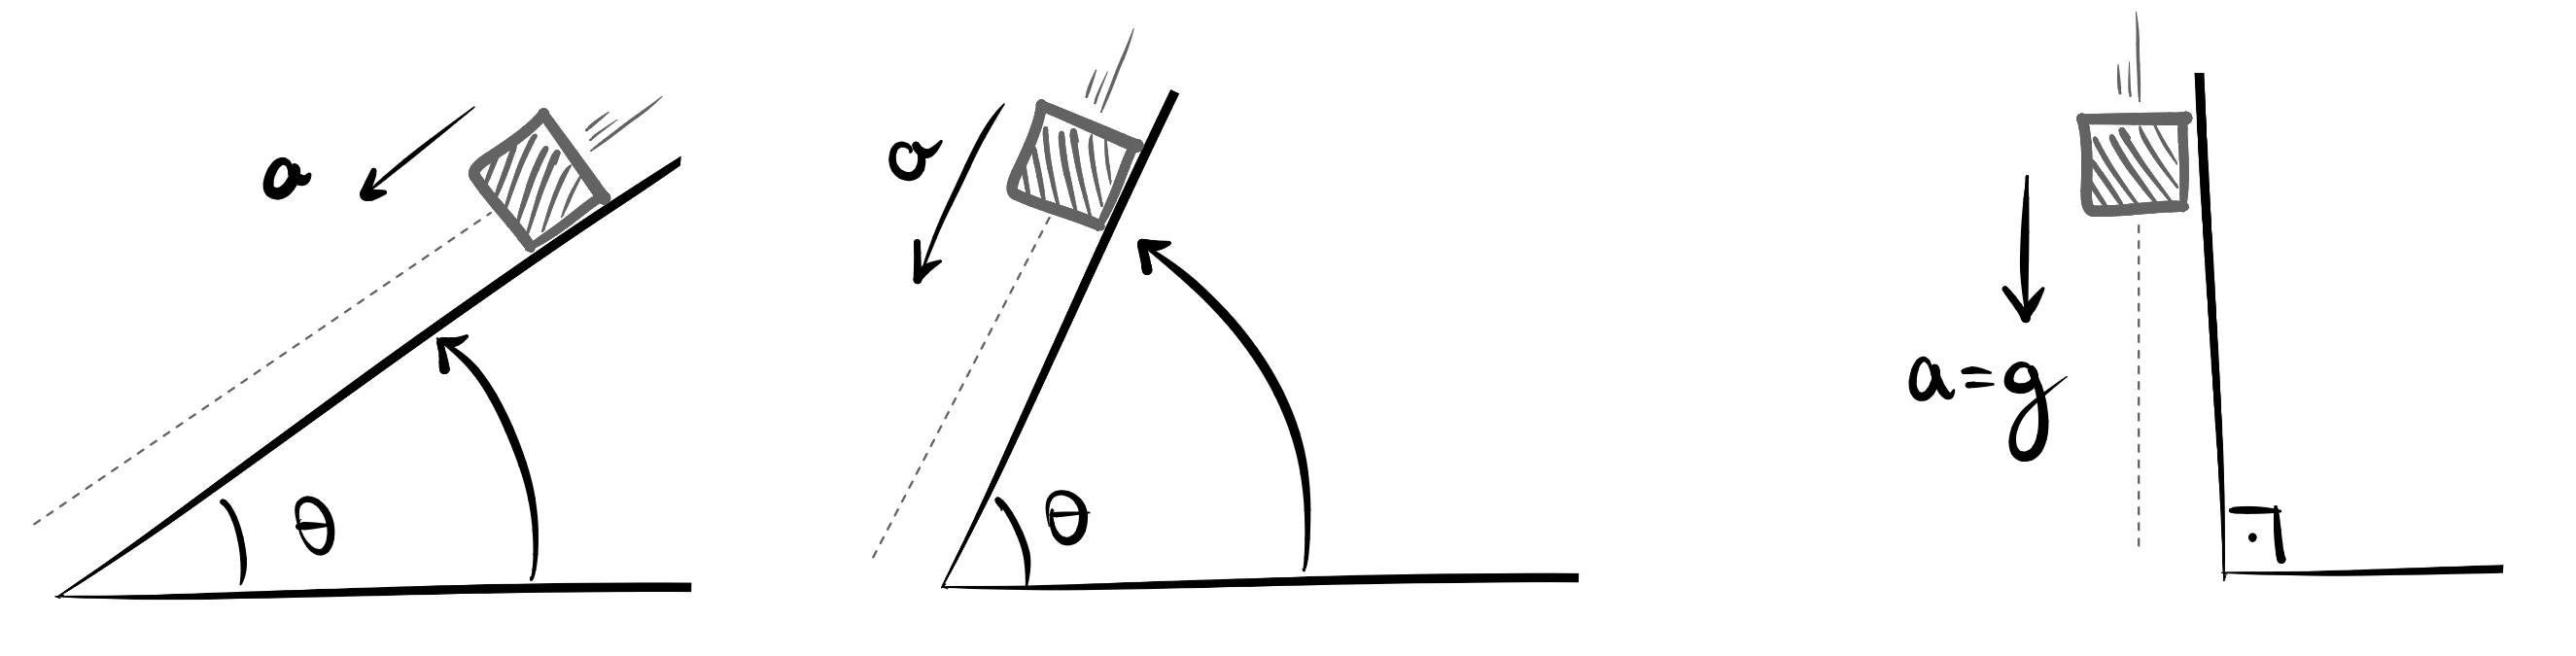
\includegraphics[width=0.8\linewidth]{imagensdinamicanewton/gsinthetacasoparticular2.png}};
  \end{scope}
\end{tikzpicture}
\captionof{figure}{Ao aumentar a inclinação do plano a aceleração da caixa deve aumentar, até atingir o valor máximo igual ao da gravidade quando a inclinação do plano for perpendicular ao chão.}
\label{fig_dinamicanewton_gsinthetacasoparticular2}
} 
\vspace{0.3cm}

Considere agora a situação da Figura \ref{fig_dinamicanewton_gsinthetacasoparticular2}. Neste caso tomamos o caminho oposto: vamos aumentar a inclinação do plano. Isso nos leva a crer que a aceleração irá aumentar, até atingir o seu valor máximo quando a inclinação do plano for de $90^\circ$: neste caso a caixa estará em queda livre, sendo sua aceleração, portanto, igual à da gravidade. Veja que é exatamente isso que a Equação \eqref{eq_dinamicanewtoniana_gsintheta} diz para $\theta=90^\circ$, uma vez que neste valor o seno é igual a 1:

$$ a = g \sin \left(\dfrac{\pi}{2}\right) = g.$$



Essa observação serve, talvez, para dois objetivos principais:

\begin{enumerate}
    \item [(i)] Mostrar que a Equação \eqref{eq_dinamicanewtoniana_gsintheta} serve para quaisquer valores de $\theta,$ ainda para situações que aparentavam não estar cobertas por ela: um plano horizontal com uma caixa em repouso ou um plano totalmente na vertical com uma caixa em queda livre.
    \item [(ii)] Evidenciar o motivo da estrutura da Equação \eqref{eq_dinamicanewtoniana_gsintheta} ser exatamente aquela. Perceba que se tivéssemos um cosseno no lugar do seno as conclusões que tiramos anteriormente não seriam corretas, o que mostraria que a equação deve estar errada. 
    
    Chamamos essa situação de análise de casos particulares: avaliamos uma equação que, a priori, vale para qualquer ângulo $\theta$, para dois valores bem específicos, no caso $\theta=0$ e $\theta = \sfrac{\pi}{2}.$ Fizemos isso porque esses dois casos particulares forneciam situações que nos eram familiares, de modo que poderíamos atestar se a tal equação de fato nos levaria ao que esperaríamos em tais situações -- o que de fato ocorre. Isso não prova que a equação está correta, é claro. Mas prova que ela, pelo menos, está de acordo com o que esperaríamos para algumas situações limite. \\
    Esse tipo de análise pode ajudar o leitor a se lembrar rapidamente da estrutura de uma equação que ele eventualmente tenha se esquecido, sem precisar, necessariamente, deduzir a equação do zero. Pode servir também para testar se uma equação encontrada está de fato correta: se ela não nos fornecer a resposta que esperamos para os casos mais simples, certamente ela está incorreta.
 \end{enumerate}

\vspace{0.3cm}

\begin{exemplo}[Nível I]\label{exemplo_dinamica1_planoinclinado01}

Um bloco é lançado com velocidade $v_0=30$ m/s de modo a subir um plano inclinado que faz um ângulo $\theta = 30^\circ$ com a horizontal.

Qual é a distância máxima que tal bloco sobe ao longo do plano?

\resolucao

A aceleração do bloco pode ser obtida pela aplicação direta da Equação \eqref{eq_dinamicanewtoniana_gsintheta} (o que eu farei, mas não recomendo que o leitor o faça, haja vista o conselho dado na subseção \textbf{Erros Comuns} sobre essa equação), de modo que o seu valor é

$$ a = g \sin \theta = 10 \cdot \sin 30^\circ = 5 \text{m/s}^2.$$

Computada a aceleração, daqui em diante torna-se um problema de Cinemática. Perceba que o valor da aceleração é constante, de modo que temos um MUV. Assim, podemos usar, por exemplo, a Equação de Torricelli:


$$ v^2 = v_0^2-2a\Delta s \implies \cancelto{0}{v^2} = 30^2 - 2 \cdot 5\Delta s \implies \Delta s = 90 \text{ m},$$

\noindent em que a velocidade final do bloco é zero uma vez que, tendo sido totalmente decelerado, ele começará a descer ao longo do plano. Assim, a máxima distância que ele sobe ao longo do plano é aquela que ele percorre até sua velocidade zerar.


\end{exemplo}


\vspace{0.3cm}


\begin{exemplo}[Nível II]\label{exemplo_dinamica1_planoinclinado02}

Considere um plano inclinado de inclinação $\theta$ em relação à horizontal e de massa $M,$ que pode se mover livremente, sem atrito, ao longo do solo. 

\vspace{0.3cm}
{
\centering
\begin{tikzpicture}
  \begin{scope}[blend mode=multiply]
    \node {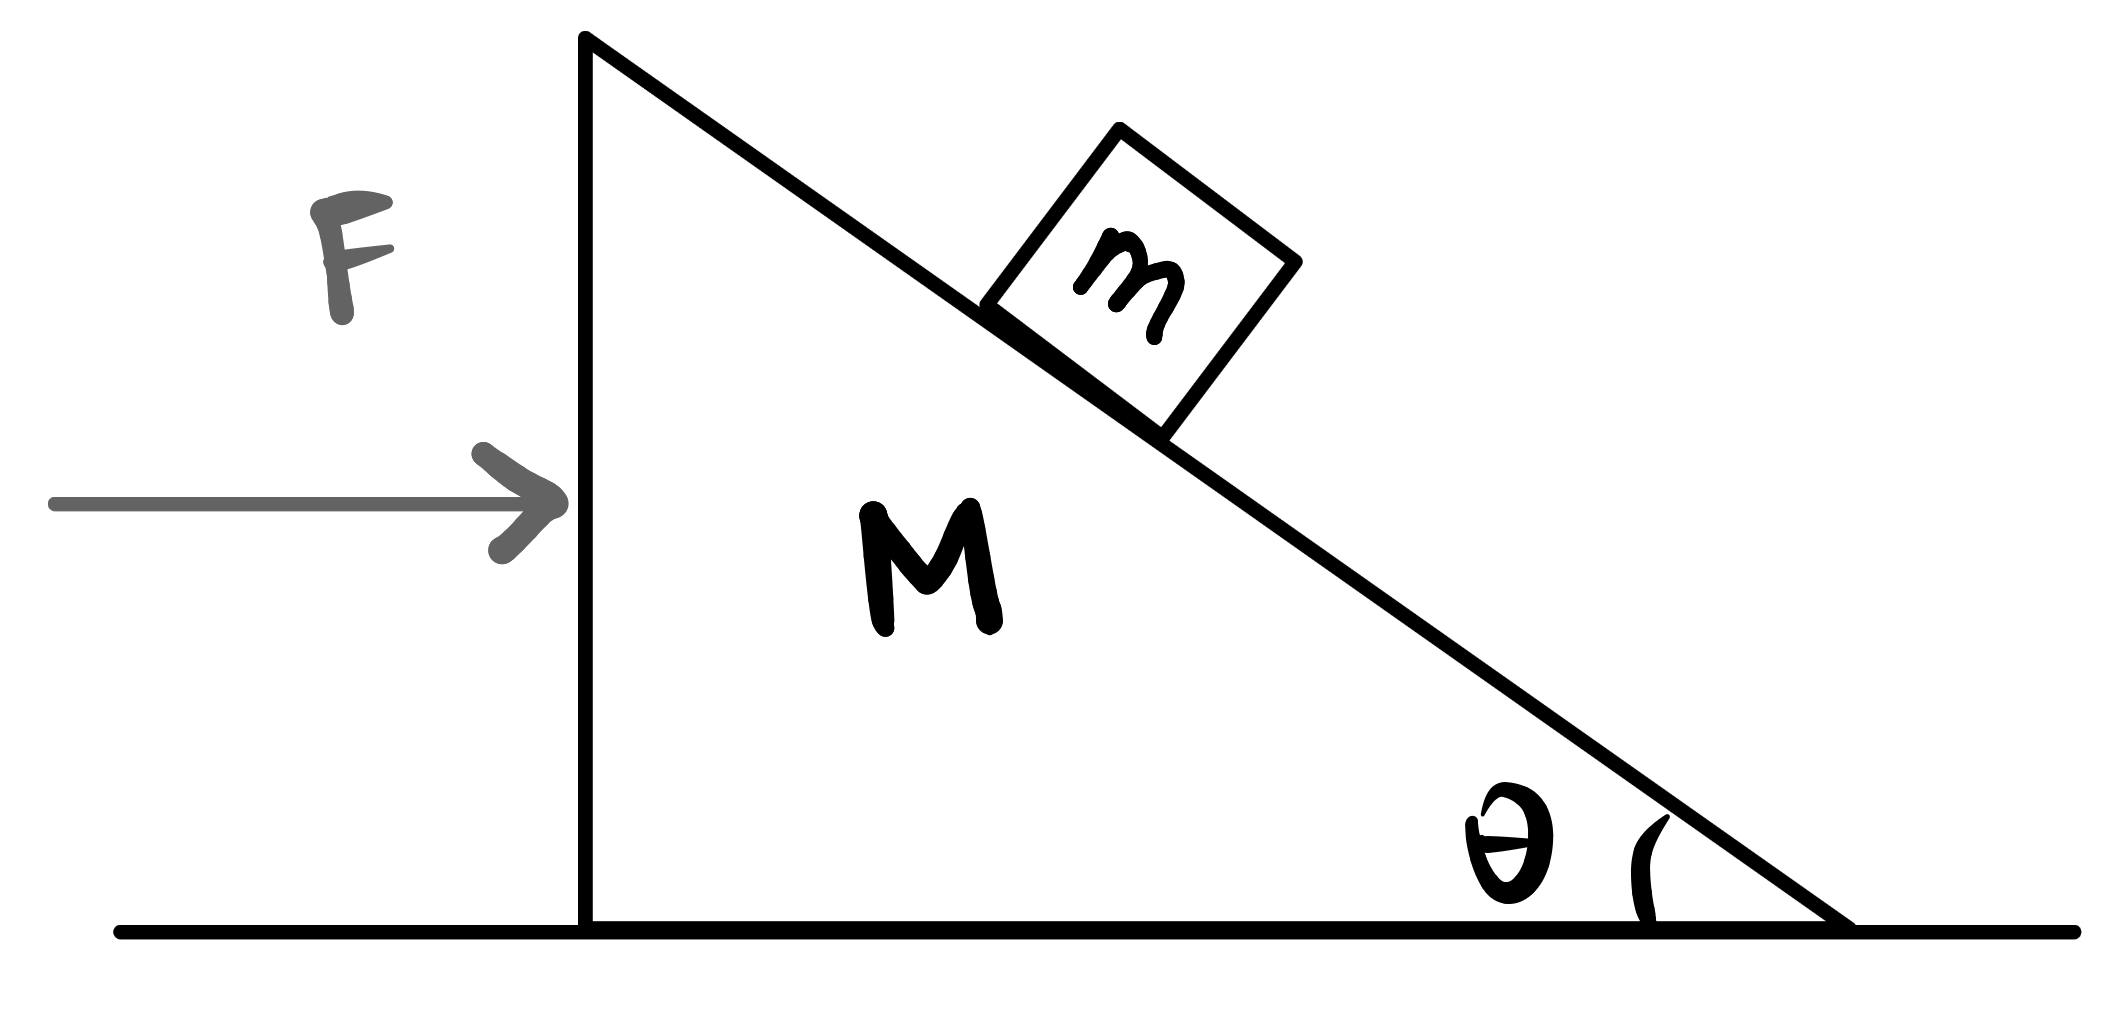
\includegraphics[width=0.35\linewidth]{imagensdinamicanewton/planoinclinadoexemplo2blocoerampa1.png}};
  \end{scope}
\end{tikzpicture}
\captionof{figure}{}
\label{fig_dinamicanewton_planoinclinadoexemplo2blocoerampa1}
} 
\vspace{0.3cm}

Em cima dele coloca-se um bloquinho de massa $m$, que também pode se mover livremente, sem atrito, ao longo do plano. Uma força $F$ é feita no plano e o acelera de tal modo que o bloquinho não se move em relação ao plano. Encontre o valor de $F.$

\resolucao

Podemos começar enxergando os dois corpos como um único corpo de massa $(m+M),$ uma vez que eles se moverão juntos, como se fosse um só corpo. 

\vspace{0.3cm}
{
\centering
\begin{tikzpicture}
  \begin{scope}[blend mode=multiply]
    \node {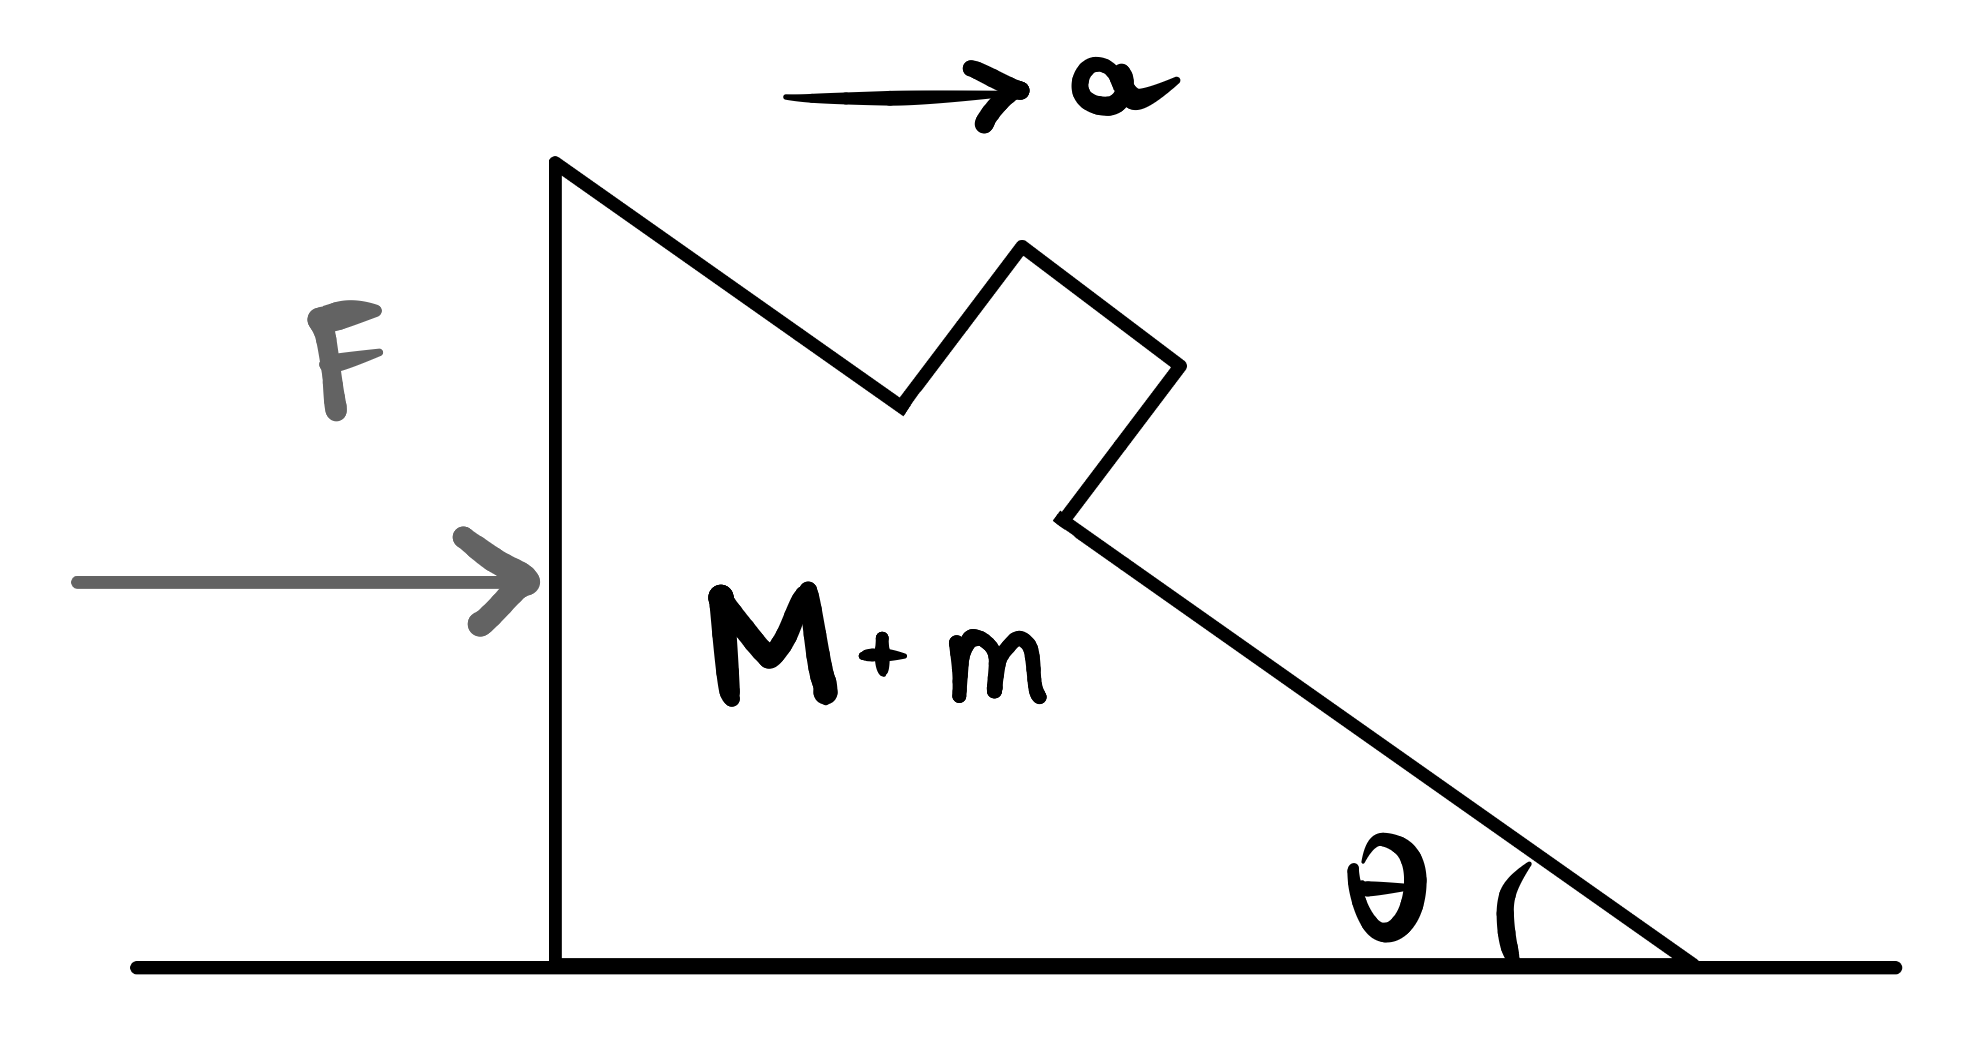
\includegraphics[width=0.35\linewidth]{imagensdinamicanewton/planoinclinadoexemplo2blocoerampa3.png}};
  \end{scope}
\end{tikzpicture}
\captionof{figure}{A rampa+bloco pode ser considerado como um corpo único.}
\label{fig_dinamicanewton_planoinclinadoexemplo2blocoerampa3}
} 
\vspace{0.3cm}


Neste caso, a força externa que acelera este sistema é a força horizontal $F$, de modo que a Segunda Lei de Newton se escreve como

$$ \boxed{F=(m+M)a.}$$

Agora, analisando separadamente as forças que atuam em cada bloco, avaliemos a resultante das forças no bloco de massa $m.$ A Figura \ref{fig_dinamicanewton_planoinclinadoexemplo2blocoerampa2} ilustra essa situação. Note que, para o bloco de massa $m,$ como ele acelera (e se move) horizontalmente para a direita, um dos eixos de decomposição das forças deverá ser o eixo horizontal -- sempre paralelo ao movimento do bloco. O outro eixo, sendo perpendicular ao primeiro, será o eixo vertical $y,$ como mostra a segunda imagem da Figura.


\vspace{0.3cm}
{
\centering
\begin{tikzpicture}
  \begin{scope}[blend mode=multiply]
    \node {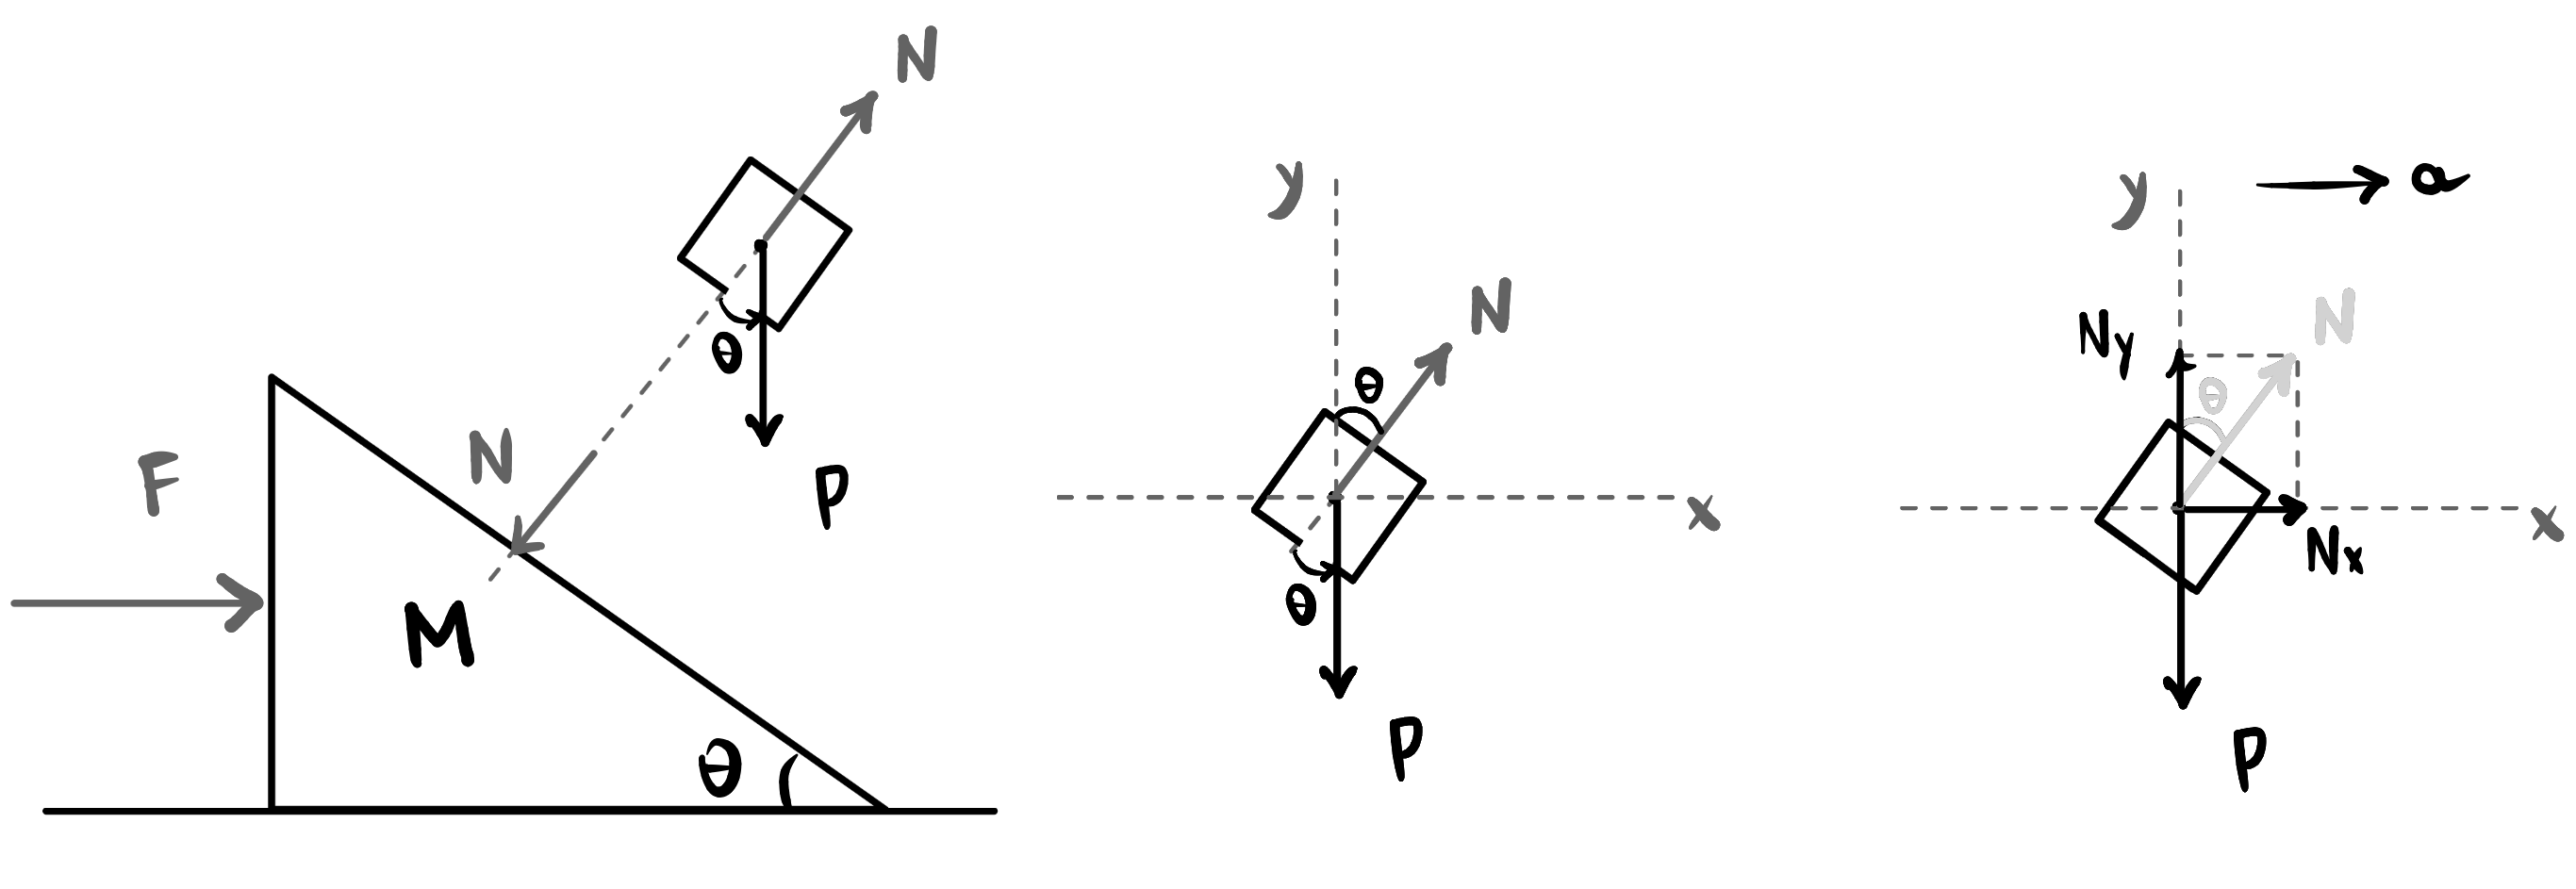
\includegraphics[width=0.95\linewidth]{imagensdinamicanewton/planoinclinadoexemplo2blocoerampa2.png}};
  \end{scope}
\end{tikzpicture}
\captionof{figure}{}
\label{fig_dinamicanewton_planoinclinadoexemplo2blocoerampa2}
} 
\vspace{0.3cm}

Assim, para o bloco de massa $m$, a Segunda Lei de Newton se escreve como:

$$
\begin{cases}
    F_{\text{R}x} = ma_x \implies N \sin \theta = ma \\
    F_{\text{R}y} = m \cancelto{0}{a_y  } =0\implies N \cos \theta = mg.
\end{cases}
$$

Dividindo as duas equações acima membro a membro, somos levados a

$$ \dfrac{\cancel N \sin \theta}{\cancel N \cos \theta} = \dfrac{\cancel ma}{\cancel mg} \implies \boxed{a = g \tan \theta.}$$

Ou seja, essa deve ser a aceleração \emph{exata} que o sistema deve ter para que o bloco de massa $m$ consiga se mover junto da rampa, sem escorregar em relação a ela.

Assim, da primeira relação obtida, é possível obter a força $F$ que viabiliza com que isso ocorra:

$$ F = (m+M)a \implies \boxed{F = (m+M)g \tan \theta.}$$
\end{exemplo}

\vspace{0.3cm}


\begin{exemplo}[Nível III]\label{exemplo_dinamica1_planoinclinado03}

Considere um plano inclinado de inclinação $\theta$ em relação à horizontal e de massa $M,$ que pode se mover livremente, sem atrito, ao longo do solo. Em cima dele coloca-se um bloquinho de massa $m$, que também pode se mover livremente, sem atrito, ao longo do plano. Ao abandonar o bloquinho, encontre o valor da aceleração do plano em relação à Terra.

\resolucao

A complexidade deste problema está no fato de que o plano
inclinado se move, de modo que não podemos simplesmente decompor o
peso do bloquinho ao longo do plano como faríamos num plano fixo. A Figura \ref{fig_dinamicanewton_planoinclinadoescorregandoex3nivelita1} ilustra essa situação: quando o bloco começa escorregar plano abaixo, o plano começa a recuar para a esquerda, com aceleração $A$. Isso faz com que, em relação à Terra, a trajetória do bloco não seja paralela ao plano inclinado.
% saída é trabalhar com as acelerações absolutas (em relação à Terra) e
% aplicar a Segunda Lei a cada corpo separadamente.

\vspace{0.3cm}
{
\centering
\begin{tikzpicture}
  \begin{scope}[blend mode=multiply]
    \node {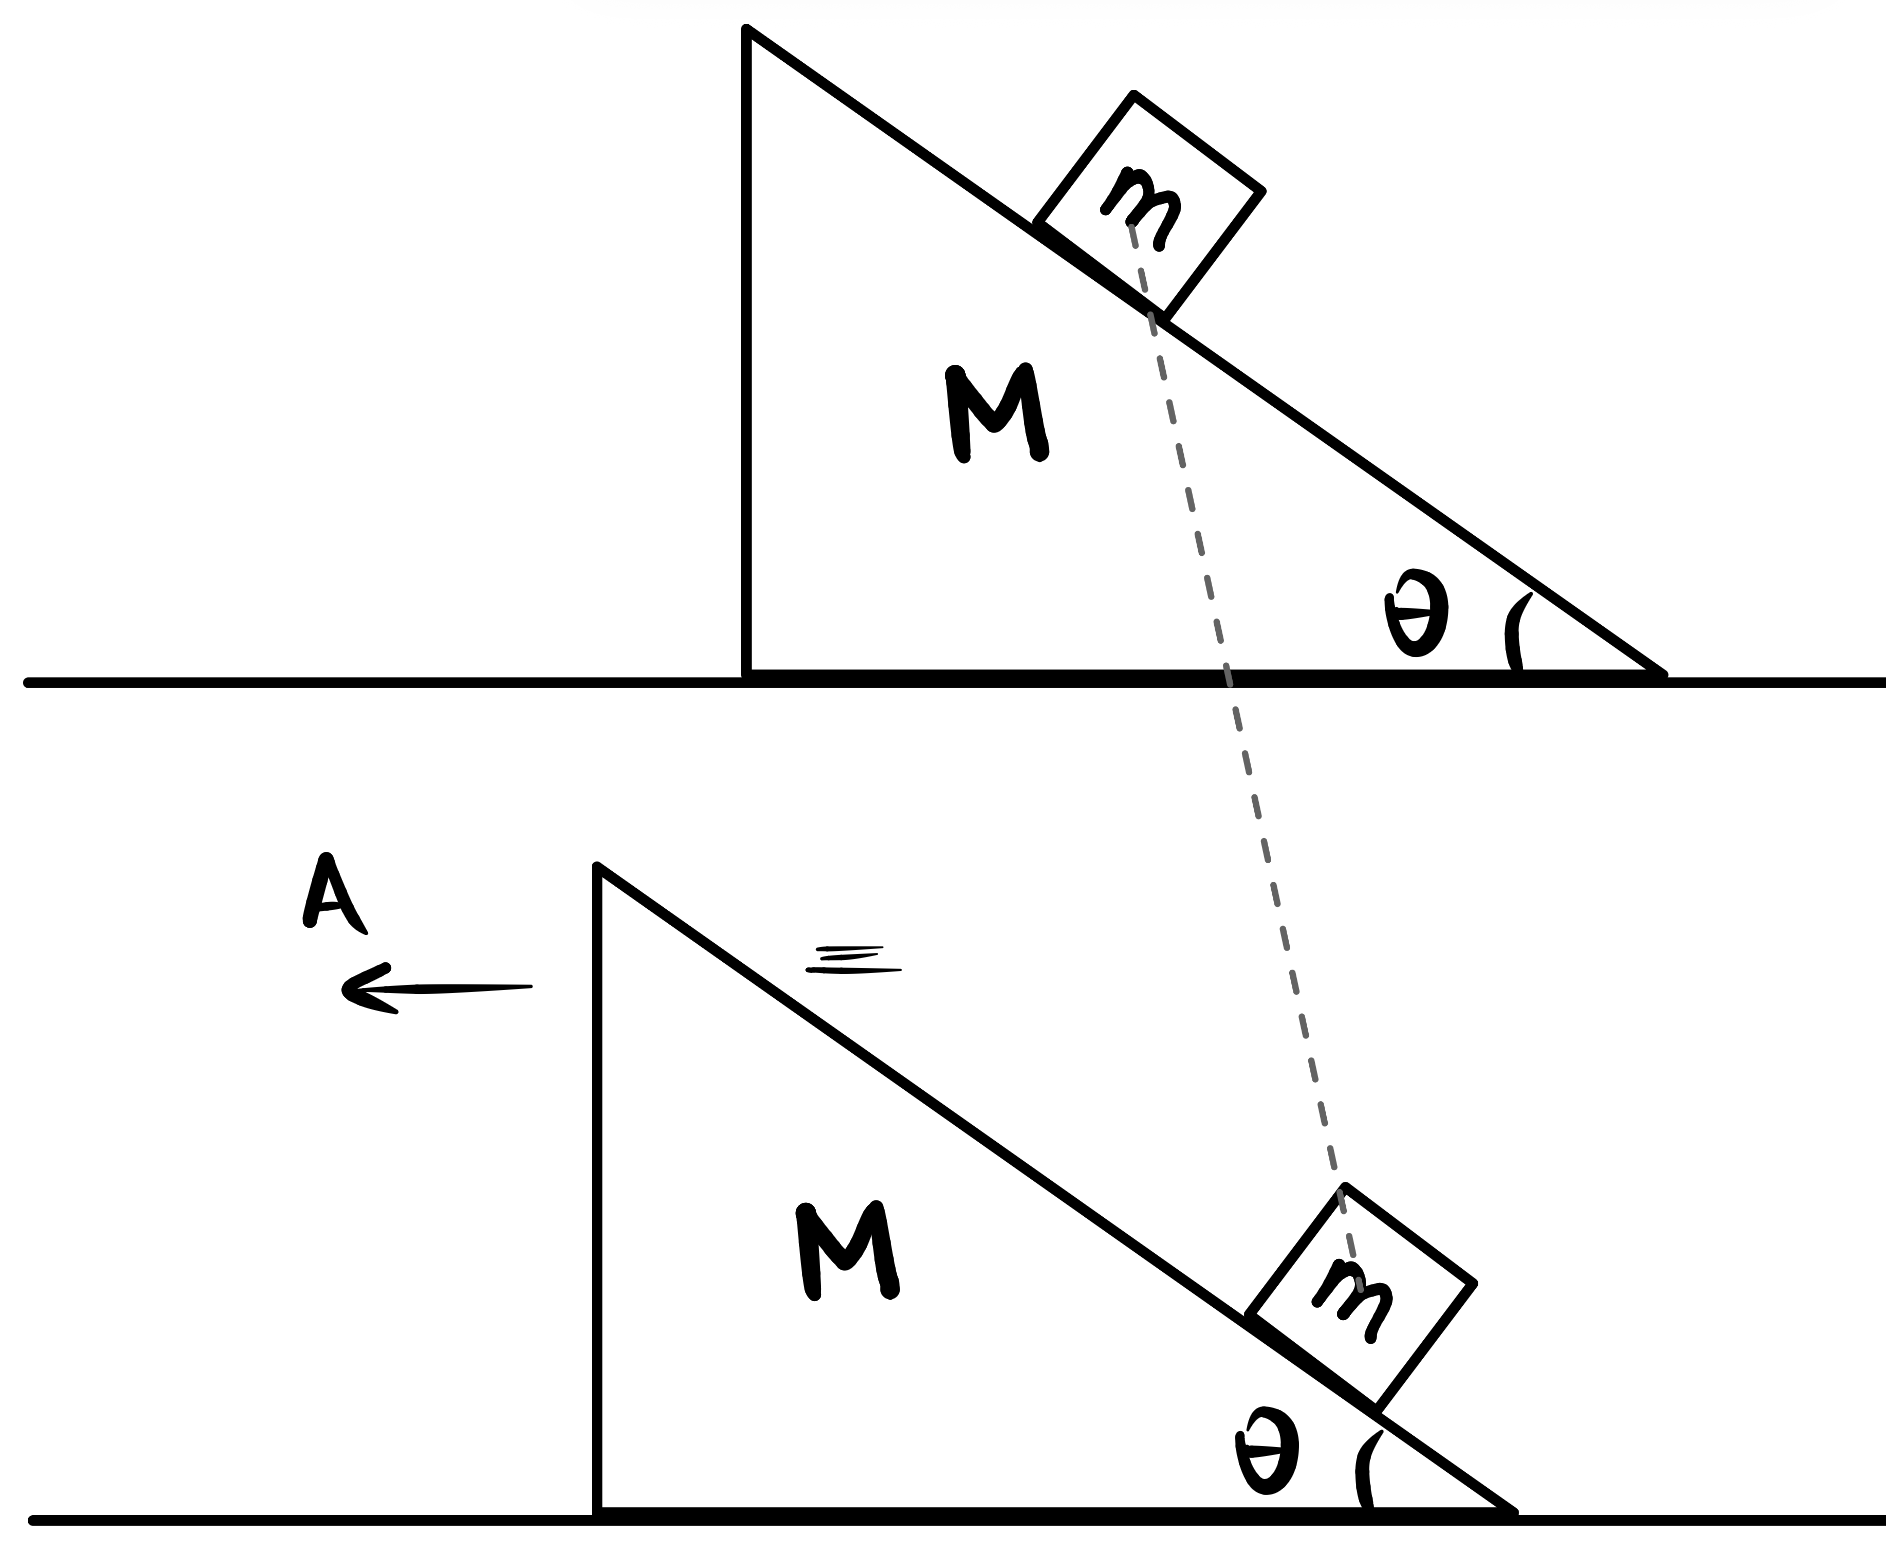
\includegraphics[width=0.45\linewidth]{imagensdinamicanewton/planoinclinadoescorregandoex3nivelita1.png}};
  \end{scope}
\end{tikzpicture}
\captionof{figure}{}
\label{fig_dinamicanewton_planoinclinadoescorregandoex3nivelita1}
} 
\vspace{0.3cm}

No referencial do plano o bloco, naturalmente, se move na direção do plano inclinado. Seja $a$ a aceleração do bloco no referencial do plano. Ela possui componentes $a_x$ e $a_y$, representadas na Figura \ref{fig_dinamicanewton_planoinclinadoescorregandoex3nivelita2}.

\vspace{0.3cm}
{
\centering
\begin{tikzpicture}
  \begin{scope}[blend mode=multiply]
    \node {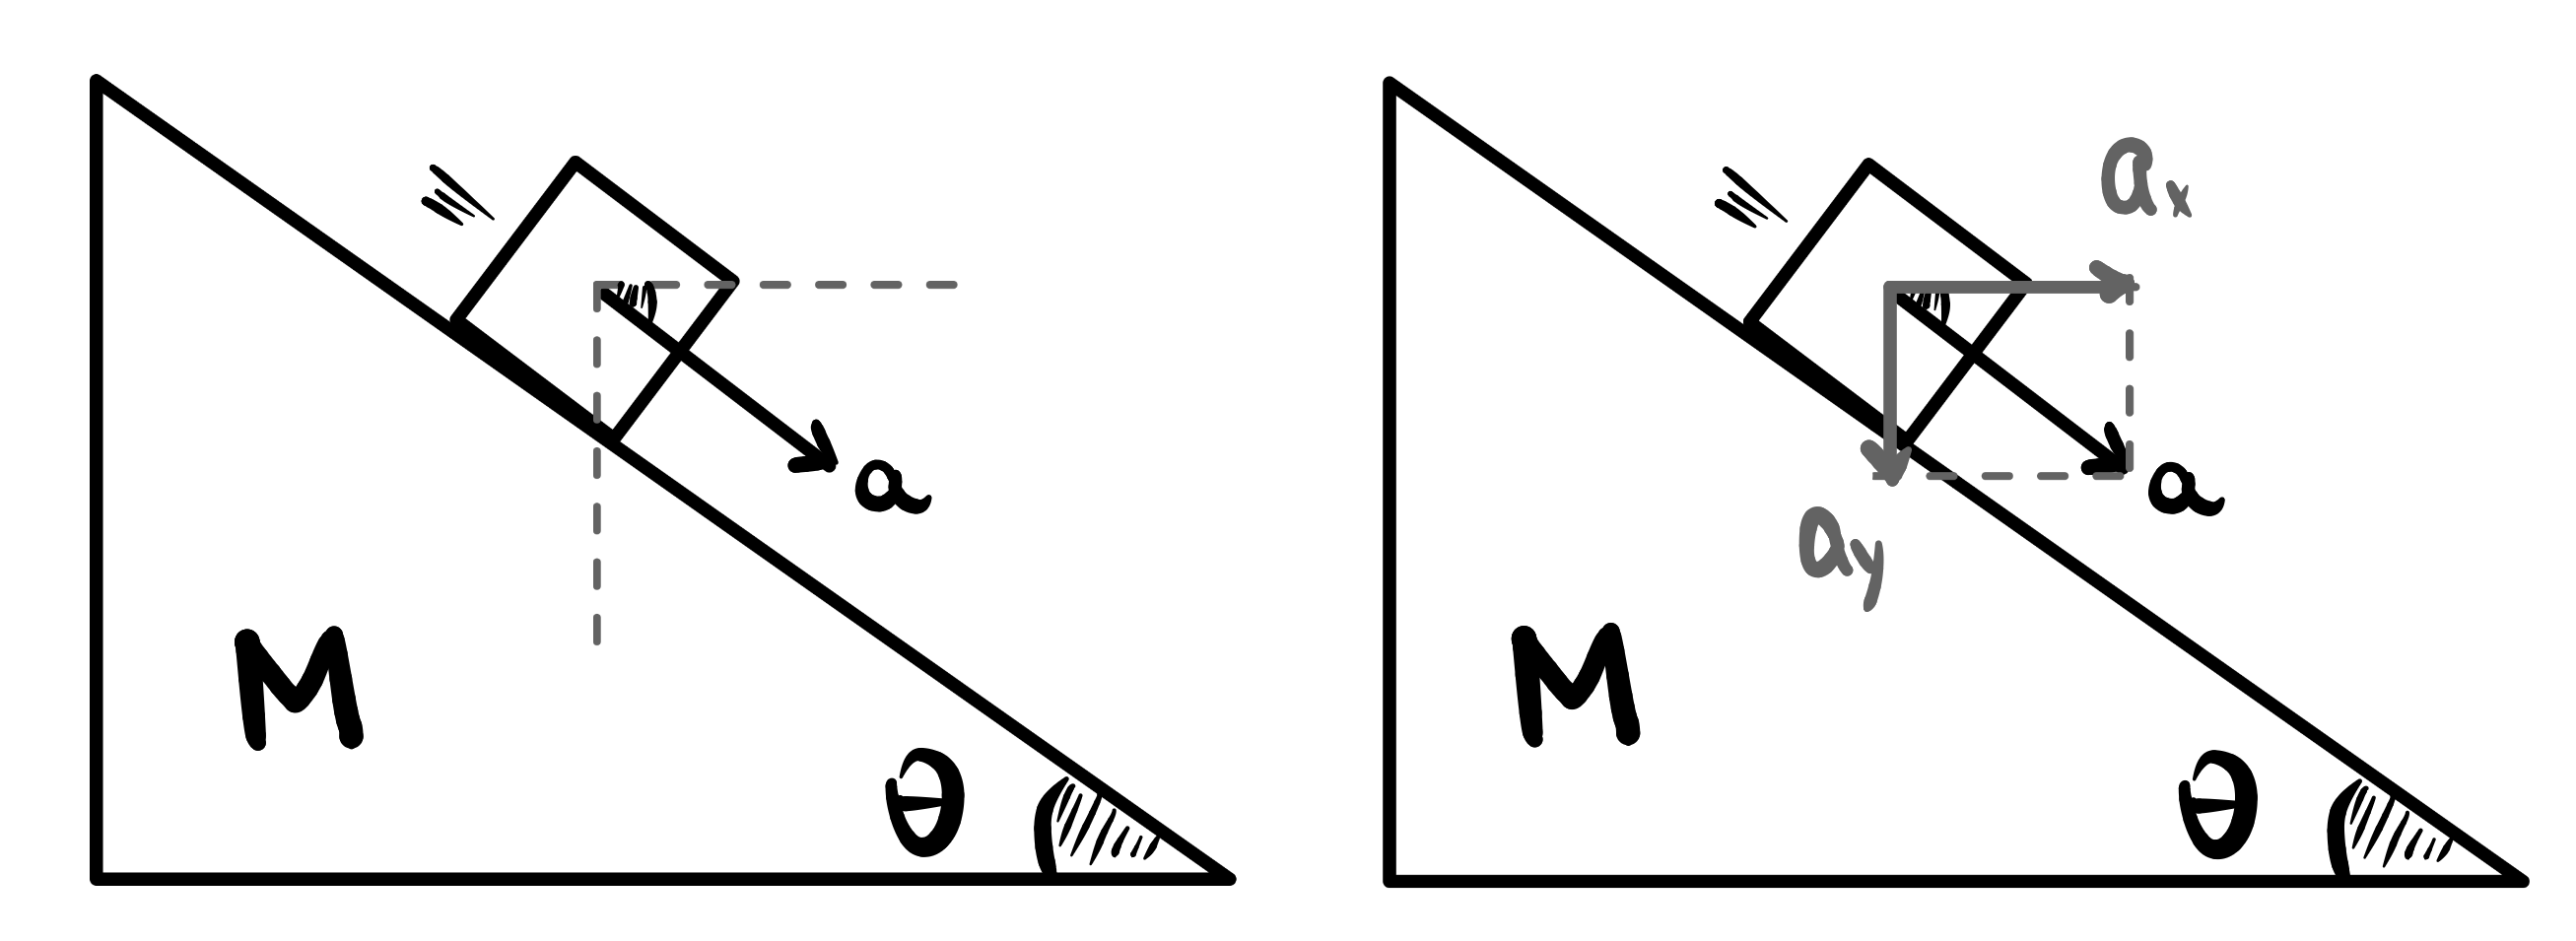
\includegraphics[width=0.55\linewidth]{imagensdinamicanewton/planoinclinadoescorregandoex3nivelita2.png}};
  \end{scope}
\end{tikzpicture}
\captionof{figure}{}
\label{fig_dinamicanewton_planoinclinadoescorregandoex3nivelita2}
} 
\vspace{0.3cm}


Sendo $A$ a aceleração do plano em relação à Terra (horizontal, para a
esquerda --- pois o bloco empurra o plano nessa direção ao deslizar).
Então a aceleração absoluta do bloquinho em relação à terra tem então:

\begin{itemize}
  \item componente horizontal: $a\cos\theta - A$ (para a direita);
  \item componente vertical: $-a\sin\theta$ (para baixo).
\end{itemize}

\medskip

A única força de contato entre o bloco e o plano é a normal $N$,
perpendicular à superfície da rampa. Ela aponta para cima e para a
direita sobre o bloco; para baixo e para a esquerda sobre o plano
(Terceira Lei). A Figura \ref{fig_dinamicanewton_planoinclinadoescorregandoex3nivelita3} mostra o diagrama de forças para cada um dos dois corpos.

\vspace{0.3cm}
{
\centering
\begin{tikzpicture}
  \begin{scope}[blend mode=multiply]
    \node {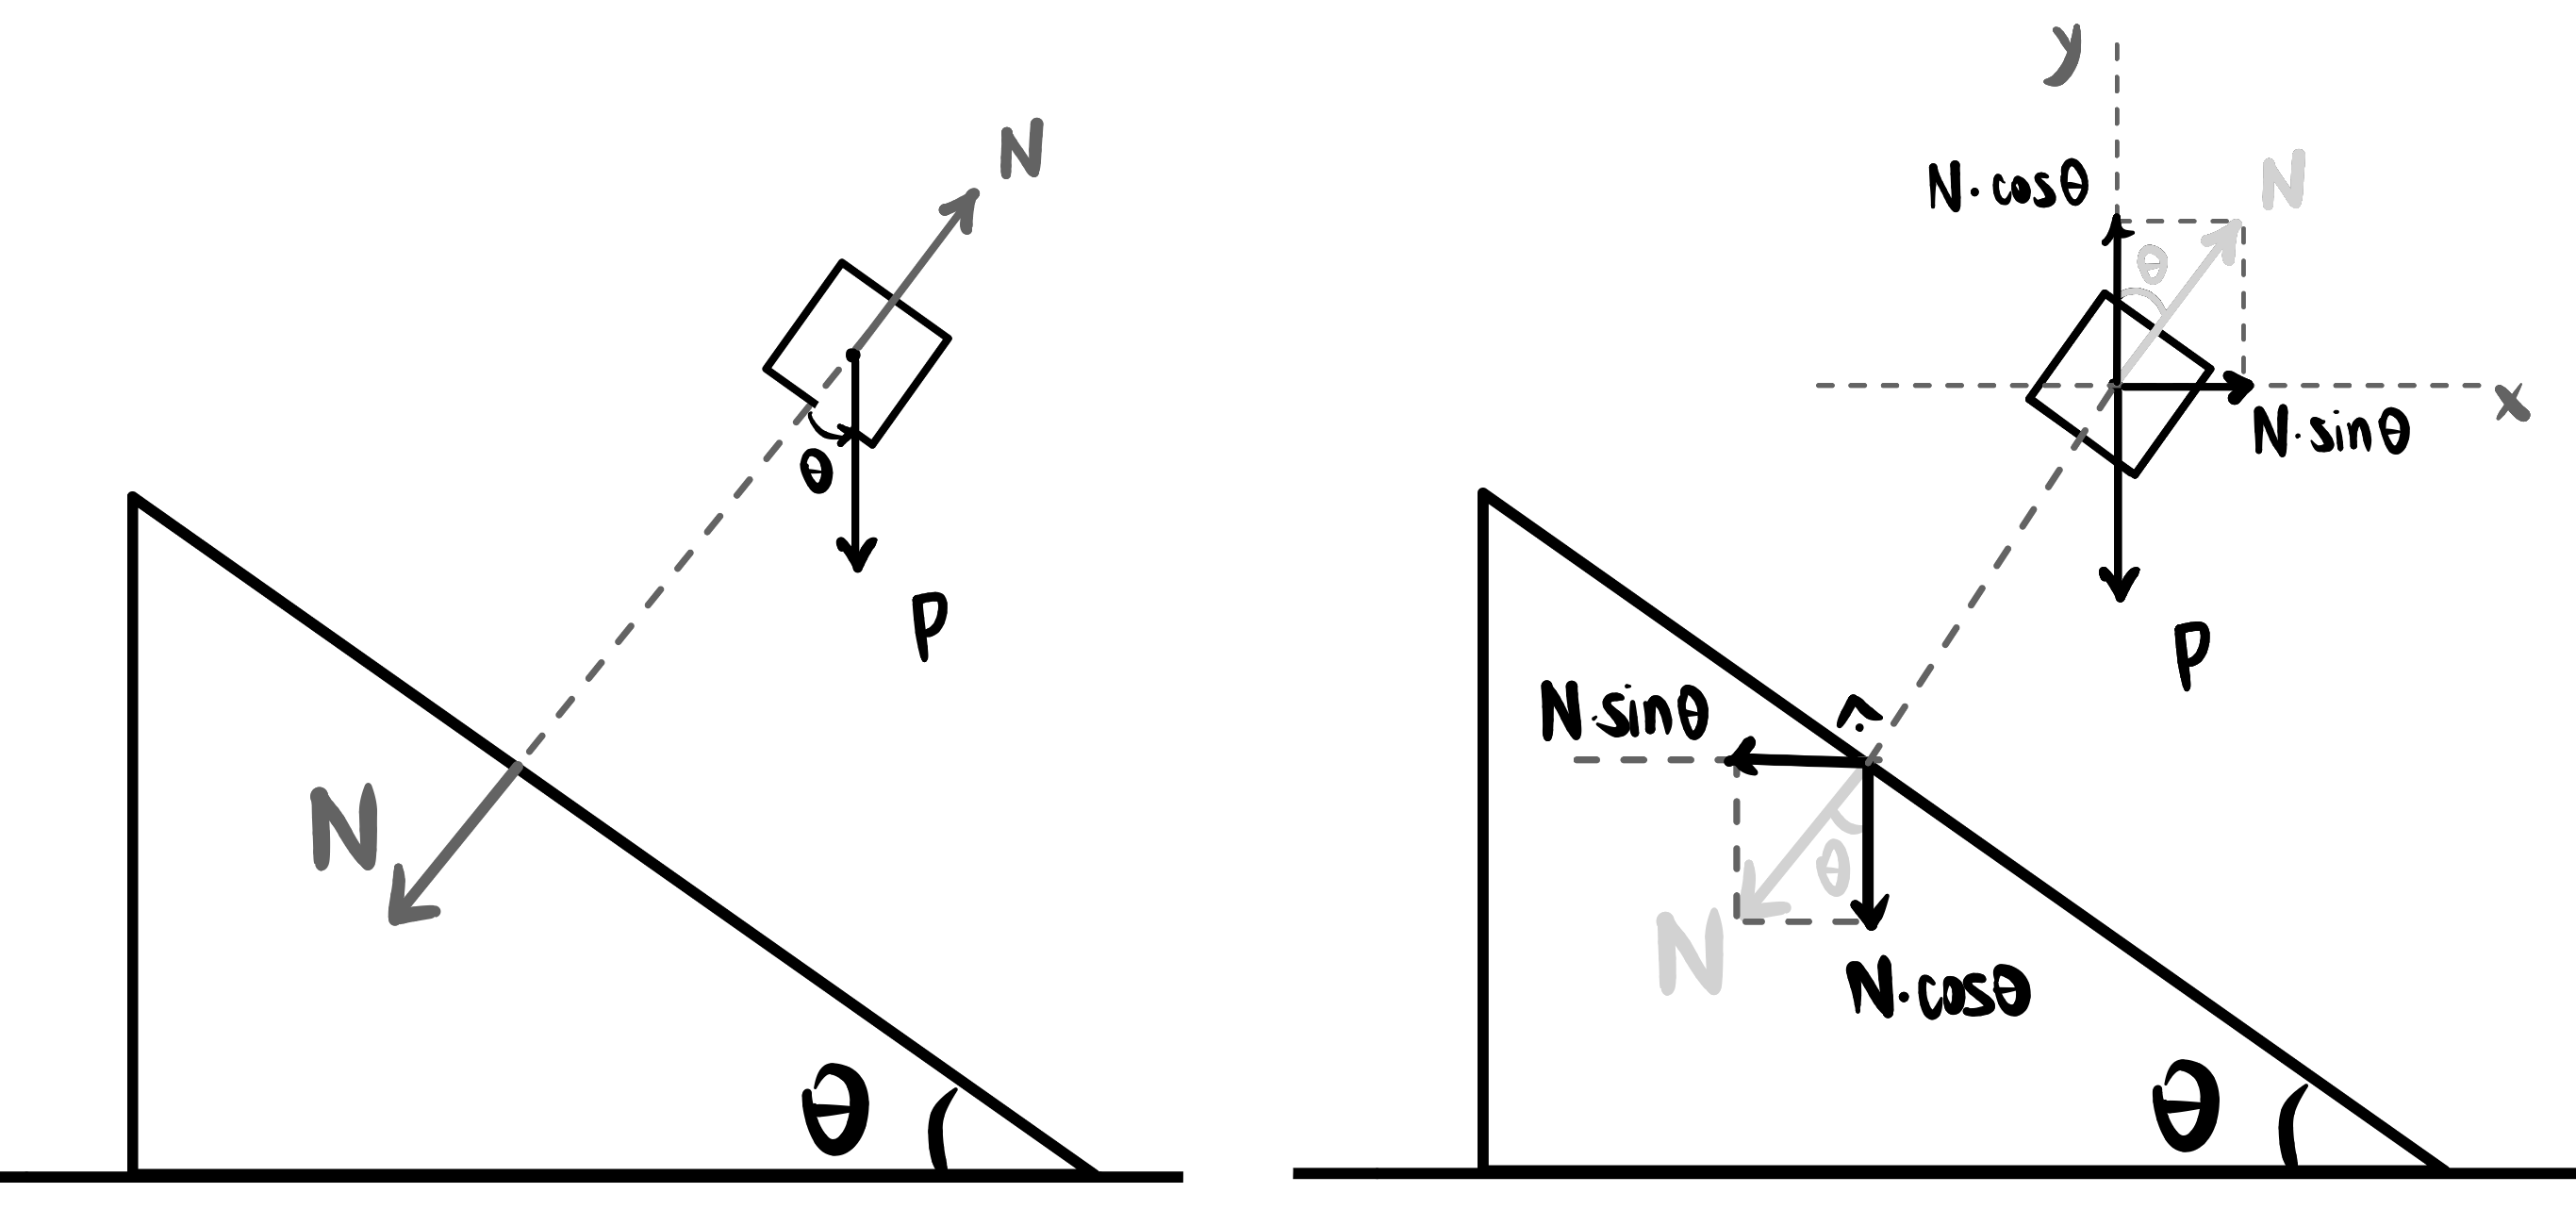
\includegraphics[width=0.8\linewidth]{imagensdinamicanewton/planoinclinadoescorregandoex3nivelita3.png}};
  \end{scope}
\end{tikzpicture}
\captionof{figure}{}
\label{fig_dinamicanewton_planoinclinadoescorregandoex3nivelita3}
} 
\vspace{0.3cm}


\medskip
Equacionando a Segunda Lei em $x$ e $y$ para o bloquinho, ter-se-á:

\begin{align}
  N\sin\theta &= m(a\cos\theta - A), \tag{1} \\
  N\cos\theta - mg &= -ma\sin\theta. \tag{2}
\end{align}

Para o plano inclinado (só a direção horizontal importa, pois ele não sai do solo):

\[
  N\sin\theta = MA. \tag{3}
\]

\medskip
De (1) e (3):

\[
  MA = m(a\cos\theta - A)
  \;\Longrightarrow\;
  A(M+m) = ma\cos\theta
  \;\Longrightarrow\;
  A = \frac{ma\cos\theta}{M+m}. \tag{4}
\]

De (2):

\[
  N = \frac{m(g - a\sin\theta)}{\cos\theta}. \tag{5}
\]

De (3) e (4):

\[
  N = \frac{MA}{\sin\theta} = \frac{Mma\cos\theta}{(M+m)\sin\theta}. \tag{6}
\]

Igualando (5) e (6):

\[
  \frac{m(g - a\sin\theta)}{\cos\theta}
  = \frac{Mma\cos\theta}{(M+m)\sin\theta}.
\]

Multiplicando ambos os lados por $\cos\theta\cdot(M+m)\sin\theta$:

\[
  (g - a\sin\theta)(M+m)\sin\theta = Ma\cos^2\theta,
\]
\[
  g(M+m)\sin\theta
  = a\bigl[M\cos^2\theta + (M+m)\sin^2\theta\bigr]
  = a\bigl[M + m\sin^2\theta\bigr].
\]

Portanto:

\[
  a = \frac{g(M+m)\sin\theta}{M + m\sin^2\theta}.
\]

Substituindo em (4):

\[
  A = \frac{m\cos\theta}{M+m}
    \cdot \frac{g(M+m)\sin\theta}{M + m\sin^2\theta},
\]

\[
  \boxed{A = \frac{mg\sin\theta\cos\theta}{M + m\sin^2\theta}.}
\]

\medskip

Vamos verificar alguns casos limite para ver se a resposta faz sentido físico.

\begin{center}
\begin{tabular}{cll}
\toprule
\textbf{Caso limite} & \textbf{Resultado} & \textbf{Interpretação} \\
\midrule
$m \to 0$      & $A \to 0$ & Sem bloco, o plano não se move \\
$M \to \infty$ & $A \to 0$ & Plano infinitamente pesado, permanece fixo \\
$\theta = 0^\circ$  & $A = 0$   & Superfície plana, sem força horizontal \\
$\theta = 90^\circ$ & $A = 0$   & Bloco cai verticalmente, não empurra o plano \\
\bottomrule
\end{tabular}
\end{center}

\noindent O máximo de $A$ ocorre num ângulo intermediário: há um
$\theta^*$ que maximiza $\sin\theta\cos\theta\,/\,(M + m\sin^2\theta)$,
revelando que existe uma inclinação ótima para a qual o plano recua
mais rapidamente. O leitor consegue encontrar essa condição e achar $A_{MAX}?$

\medskip

Por fim, cabe comentarmos um outro tipo de solução para este mesmo problema, que reside em um certo \emph{vínculo} entre o movimento do bloco e da rampa: como o bloco sempre permanece em contato com a rampa isso significa que a aceleração relativa entre esses corpos na direção perpendicular à rampa é zero:


$$ A \sin \theta = a_x \sin \theta - a_y \cos \theta. \tag{7}$$

As Equações $(1)$ e $(2)$ são simplesmente a Segunda Lei de Newton para o bloquinho na horizontal e vertical, respectivamente. De onde tiramos que:

$$ N \sin \theta = ma_x \implies \boxed{a_x = \dfrac{N \sin \theta}{m},} \tag{8}$$

$$ N \cos \theta - mg = ma_y \implies \boxed{a_y = \dfrac{N \cos \theta  - mg}{m}.} \tag{9}$$


De $(3)$ extraímos que 

$$ A = \dfrac{N \sin \theta }{M} \tag {10}.$$

Substituindo (8), (9) e (10) na Equação do vínculo (7):


$$ \dfrac{N \sin \theta }{M} \sin \theta = \dfrac{N \sin \theta}{m} \sin \theta - \dfrac{(N \cos \theta  - mg)}{m}\cos \theta,$$

\noindent que, desenvolvendo, nos leva a

$$N = \frac{gmM\cos\theta}{M + m\sin^2\theta}.$$

Substituindo em (10):

$$\boxed{A = \frac{gm\sin\theta\cos\theta}{M + m\sin^2\theta}.}$$

A sacada dessa solução está no vínculo (7): ao exigir que a aceleração relativa não tenha componente normal, eliminamos completamente a aceleração relativa $a$ do sistema
--- ela sequer aparece. O problema se reduz a três equações de Newton em três incógnitas, e fecha direto.

\end{exemplo}



\begin{secnivel}[Condição de Equilíbrio]{I}{Condição de Equilíbrio}
  
  \eqLdois{def}{eq_newton_equilibriof=0}{F_R=0}

\end{secnivel}







\secgfe{De onde vem}

Vamos ampliar o nosso vocabulário: em Física, quando se diz que um corpo está em equilíbrio, queremos dizer que a resultante das forças que nele atuam é nula. Essa é uma definição: equilíbrio é a condição em que um corpo está tal que a Equação \eqref{eq_newton_equilibriof=0} é satisfeita.



\secgfe{Onde é usada}

Em diversos contextos iremos lidar com corpos em equilíbrio -- seja em repouso ou em MRU. O importante aqui é que o leitor esteja familiarizado com tal termo e entenda, fisicamente, o que isso significa. Ao se deparar com uma situação que diz que um certo corpo está em equilíbrio, a Equação \eqref{eq_newton_equilibriof=0} precisa vir na sua mente de imediato -- ela é versão matemática que define o que é a condição de equilíbrio.



\secgfe{Erros comuns}

O erro mais comum é assumir que, por estar em equilíbrio, o corpo tem que estar, necessariamente, parado. Como já vimos no estudo da Segunda Lei de Newton na Seção \ref{secao_mecanicanewtoniana_segundaleinewton}, diferente do que Aristóteles pensava, se a força resultante atuando em um corpo é nula, existem não apenas uma, mas duas situações que satisfazem tal condição:

\begin{enumerate}
    \item [(i)] Repouso.

     O corpo pode estar, de fato, parado. Chamamos essa condição de \textbf{equilíbrio estático}.

    \item [(ii)] Movimento Retilíneo Uniforme (MRU).

    Como observado por Galileu, existe um outro estado de movimento inercial além do repouso: o MRU -- um estado de movimento na ausência de forças. Assim, se $F_R=0,$ o corpo pode também estar em MRU, e permaneceria indefinidamente em tal estado a menos que uma força se manifeste para alterar seu estado de movimento. Isso é justamente o que diz a Primeira Lei de Newton.

    Tal condição é chamada de \textbf{equilíbrio dinâmico.}
\end{enumerate}



\secgfe{Observações}

Dentro da condição de equilíbrio estático, ou seja, quando já se sabe que o corpo está em repouso, existem algumas situações distintas que merecem ser destacadas. Considere a Figura \ref{fig_newton_equilibrioestavel1}, em que temos, nas três situações, a bolinha em equilíbrio estático.

\vspace{0.3cm}
{
\centering
\begin{tikzpicture}
  \begin{scope}[blend mode=multiply]
    \node {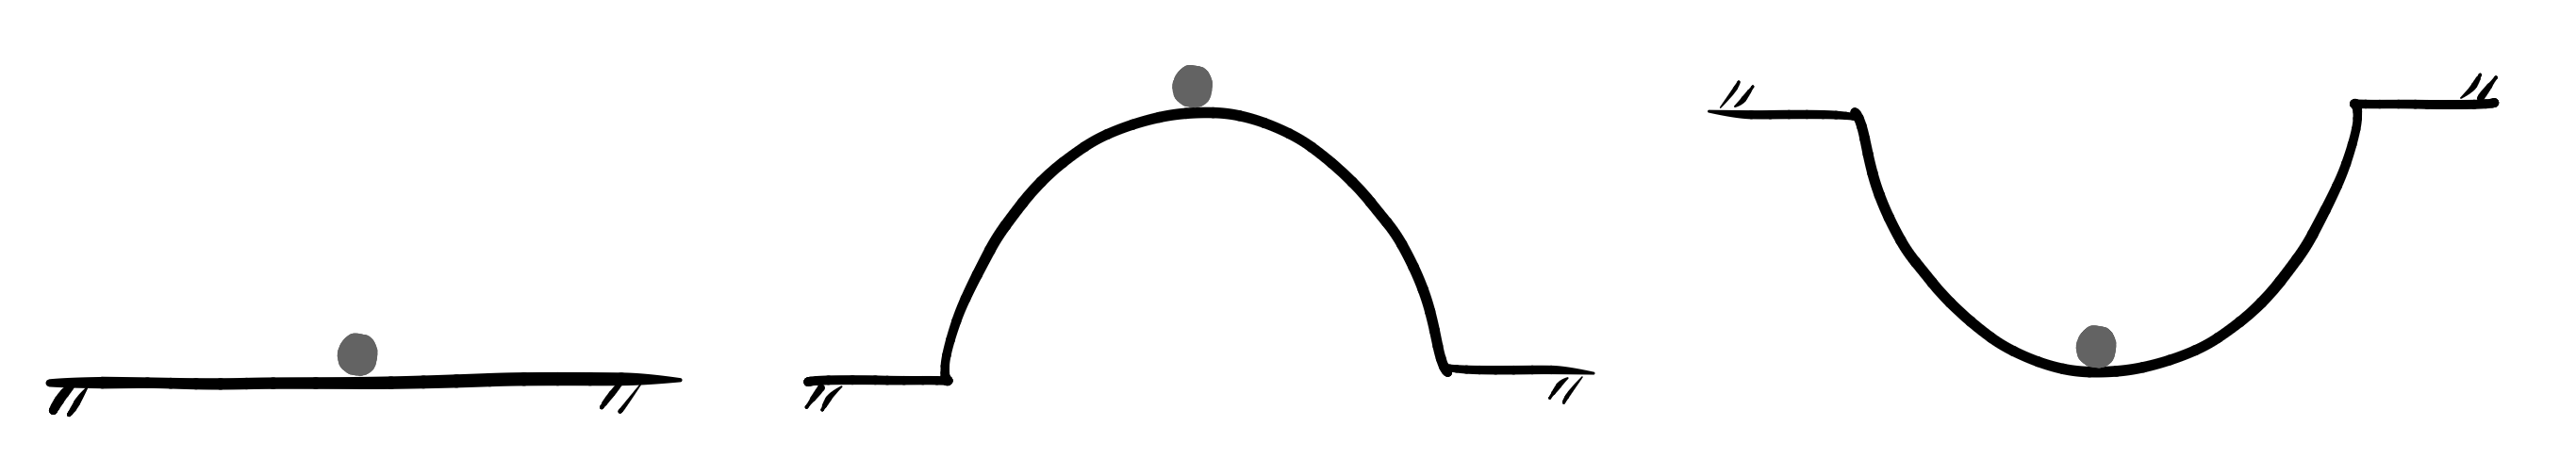
\includegraphics[width=0.8\linewidth]{imagensdinamicanewton/equilibrioestavel1.png}};
  \end{scope}
\end{tikzpicture}
\captionof{figure}{Três corpos em condição de equilíbrio estático.}
\label{fig_newton_equilibrioestavel1}
} 
\vspace{0.3cm}

Qual seria a diferença entre cada uma delas? Ora, se nas três situações trata-se de uma condição de equilíbrio, então certamente as forças atuantes precisam se anular. A Figura \ref{fig_newton_equilibrioestavel2} ilustra isso: por conta de seu peso a bolinha comprime o solo, fazendo nele uma força normal. Pela Terceira Lei o solo reage, fazendo uma força normal na bolinha, que deve ser anulada pelo seu peso, a fim de garantir a condição de equilíbrio.


\vspace{0.3cm}
{
\centering
\begin{tikzpicture}
  \begin{scope}[blend mode=multiply]
    \node {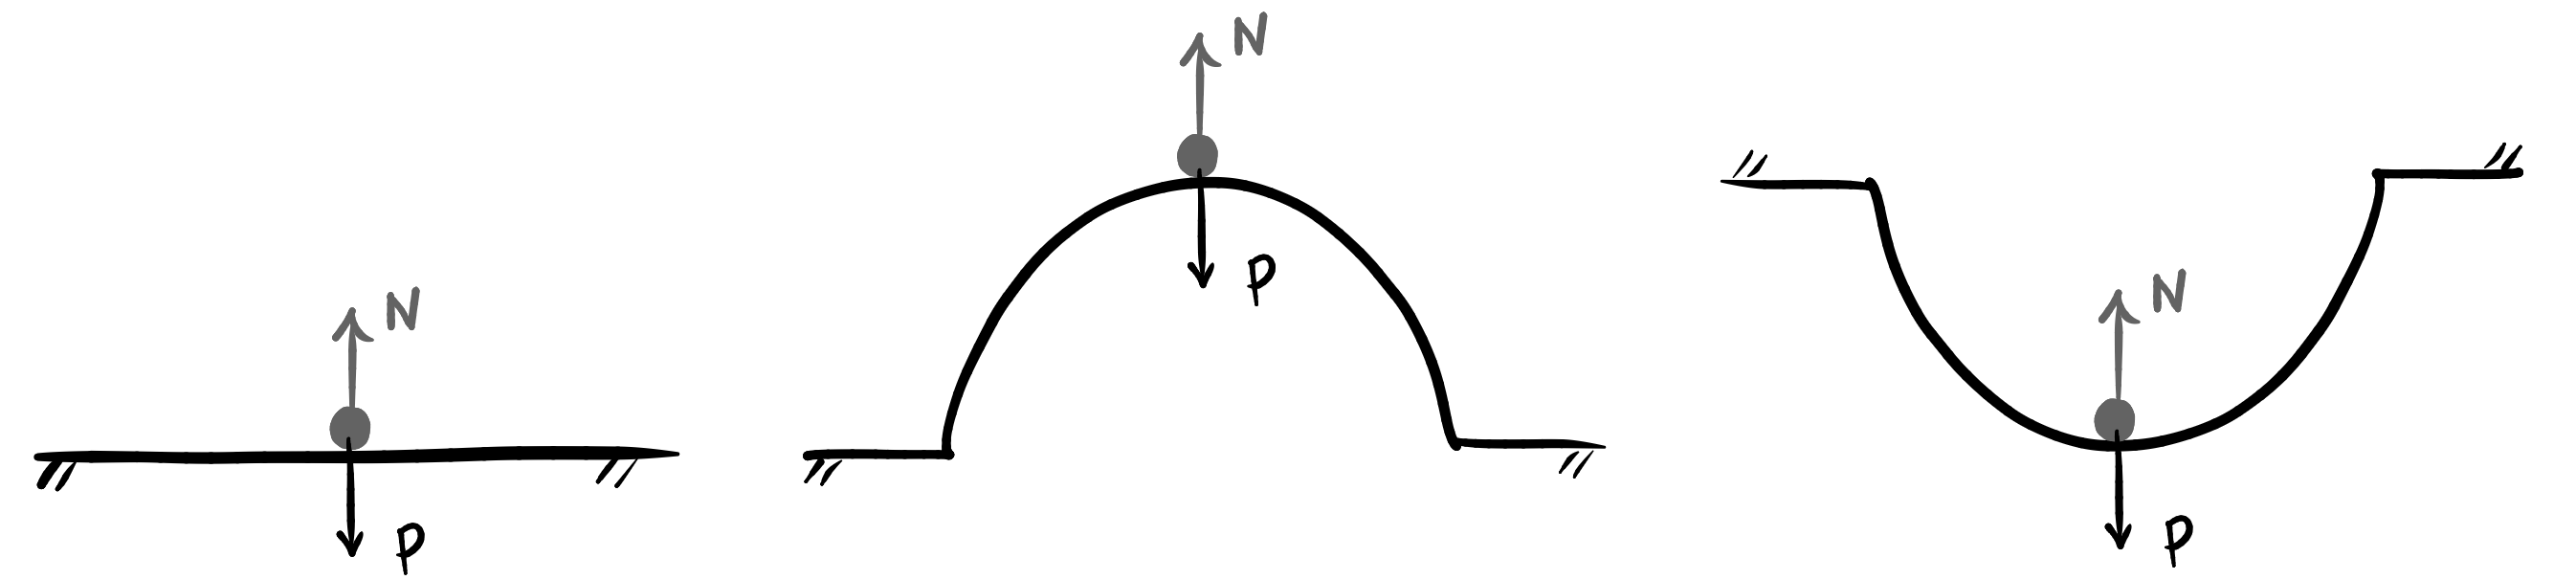
\includegraphics[width=0.8\linewidth]{imagensdinamicanewton/equilibrioestavel2.png}};
  \end{scope}
\end{tikzpicture}
\captionof{figure}{A condição de equilíbrio impõe que $F_R=0$, ou seja, a força normal anula o peso.}
\label{fig_newton_equilibrioestavel2}
} 
\vspace{0.3cm}

Note, contudo, que existe uma diferença entre as três situações da Figura \ref{fig_newton_equilibrioestavel1}. Não tem a ver com a dinâmica das forças, mas sim com o que acontece com o sistema ao ser levemente perturbado. Considere a situação de afastar levemente a bolinha da sua posição inicial de equilíbrio, isto é, retirá-la de onde ela está e colocá-la e uma posição, digamos, um centímetro para a direita. Na situação da primeira imagem ela voltaria a ficar em equilíbrio nessa mesma posição. Contudo, na situação da segunda imagem -- no topo do morro -- ao se deslocar de muito pouco para a direita a bolinha começaria a rolar morro abaixo. Tal situação é chamada, portanto, de \textbf{equilíbrio instável:} ao ser levemente perturbada da sua posição de equilíbrio a bolinha tende a se afastar de tal posição.

Já na situação da terceira imagem, no fundo do vale, ao se deslocar de muito pouco para a direita a bolinha começaria a rolar de volta para baixo, tendendo a volta para a sua posição anterior. Tal situação é chamada, portanto, de \textbf{equilíbrio estável:} ao ser levemente perturbada da sua posição de equilíbrio a bolinha tende a retornar para tal posição. Tal situação dará origem a movimentos oscilatórios, em que o corpo poderá oscilar em torno da sua posição de equilíbrio. 

A Figura \ref{fig_newton_rolypoly} ilustra um brinquedo, o \emph{João Bobo,} que representa bem a situação de equilíbrio estável: ao golpear e tombar o brinquedo ele sempre retorna à sua posição inicial de equilíbrio. Isso tem a ver com a posição do seu centro de massa, assunto que será discutido em detalhes no estudo da Equação \eqref{eq_newtonrotacao_posicaocentrodemassa}.

\vspace{0.3cm}
{
\centering
\begin{tikzpicture}
  \begin{scope}[blend mode=multiply]
    \node {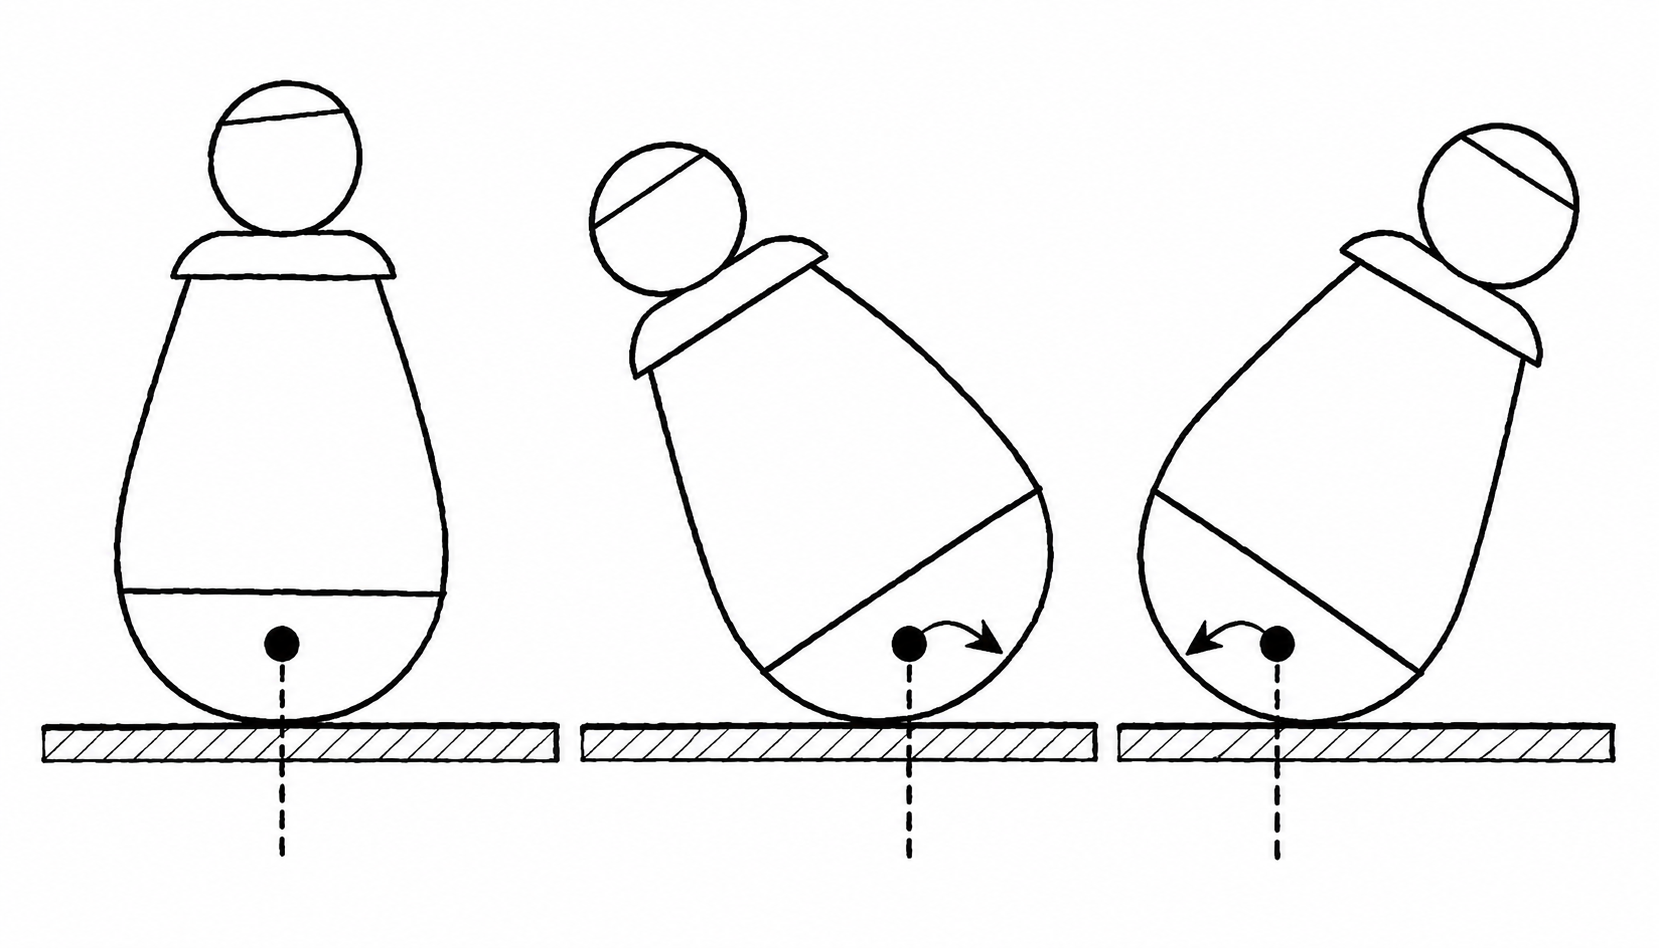
\includegraphics[width=0.5\linewidth]{imagensdinamicanewton/joaobobo.png}};
  \end{scope}
\end{tikzpicture}
\captionof{figure}{Brinquedo que ilustra a condição de equilíbrio estável.}
\label{fig_newton_rolypoly}
} 
\vspace{0.3cm}



Já a situação da primeira imagem é chamada de \textbf{equilíbrio indiferente}: o corpo não tende a retornar nem se afastar da sua posição inicial quando levemente perturbado.

\vspace{0.3cm}

\begin{exemplo}[Nível I]\label{exemplo_newton_equilibrio01}

Um bloco está apoiado sob um plano inclinado, fixo ao solo, que faz um ângulo $\theta = 45^\circ $ com a horizontal. O bloco está preso, na sua parte superior, por um fio ideal, paralelo ao plano inclinado, fixado na sua parte superior.

Se a tração máxima que o fio suporta é igual a $282$ N, qual é o maior valor de massa $m$ do bloco para que ele fique em equilíbrio?

\resolucao

A Figura \ref{fig_newton_planoinclinadoequilibrio} ilustra a situação do problema. Na segunda imagem já desenhamos todas as forças que atuam no bloco -- já decompostas nos eixos normal ($y$) e paralelo ($x)$ ao plano.

As forças de tração no fio e a força normal feita pelo plano no bloco não precisam ser decompostas uma vez que já estão alinhadas com tais eixos. A decomposição da força peso é exatamente aquela feita no desenvolvimento da Equação \eqref{eq_dinamicanewtoniana_gsintheta}.

\vspace{0.3cm}
{
\centering
\begin{tikzpicture}
  \begin{scope}[blend mode=multiply]
    \node {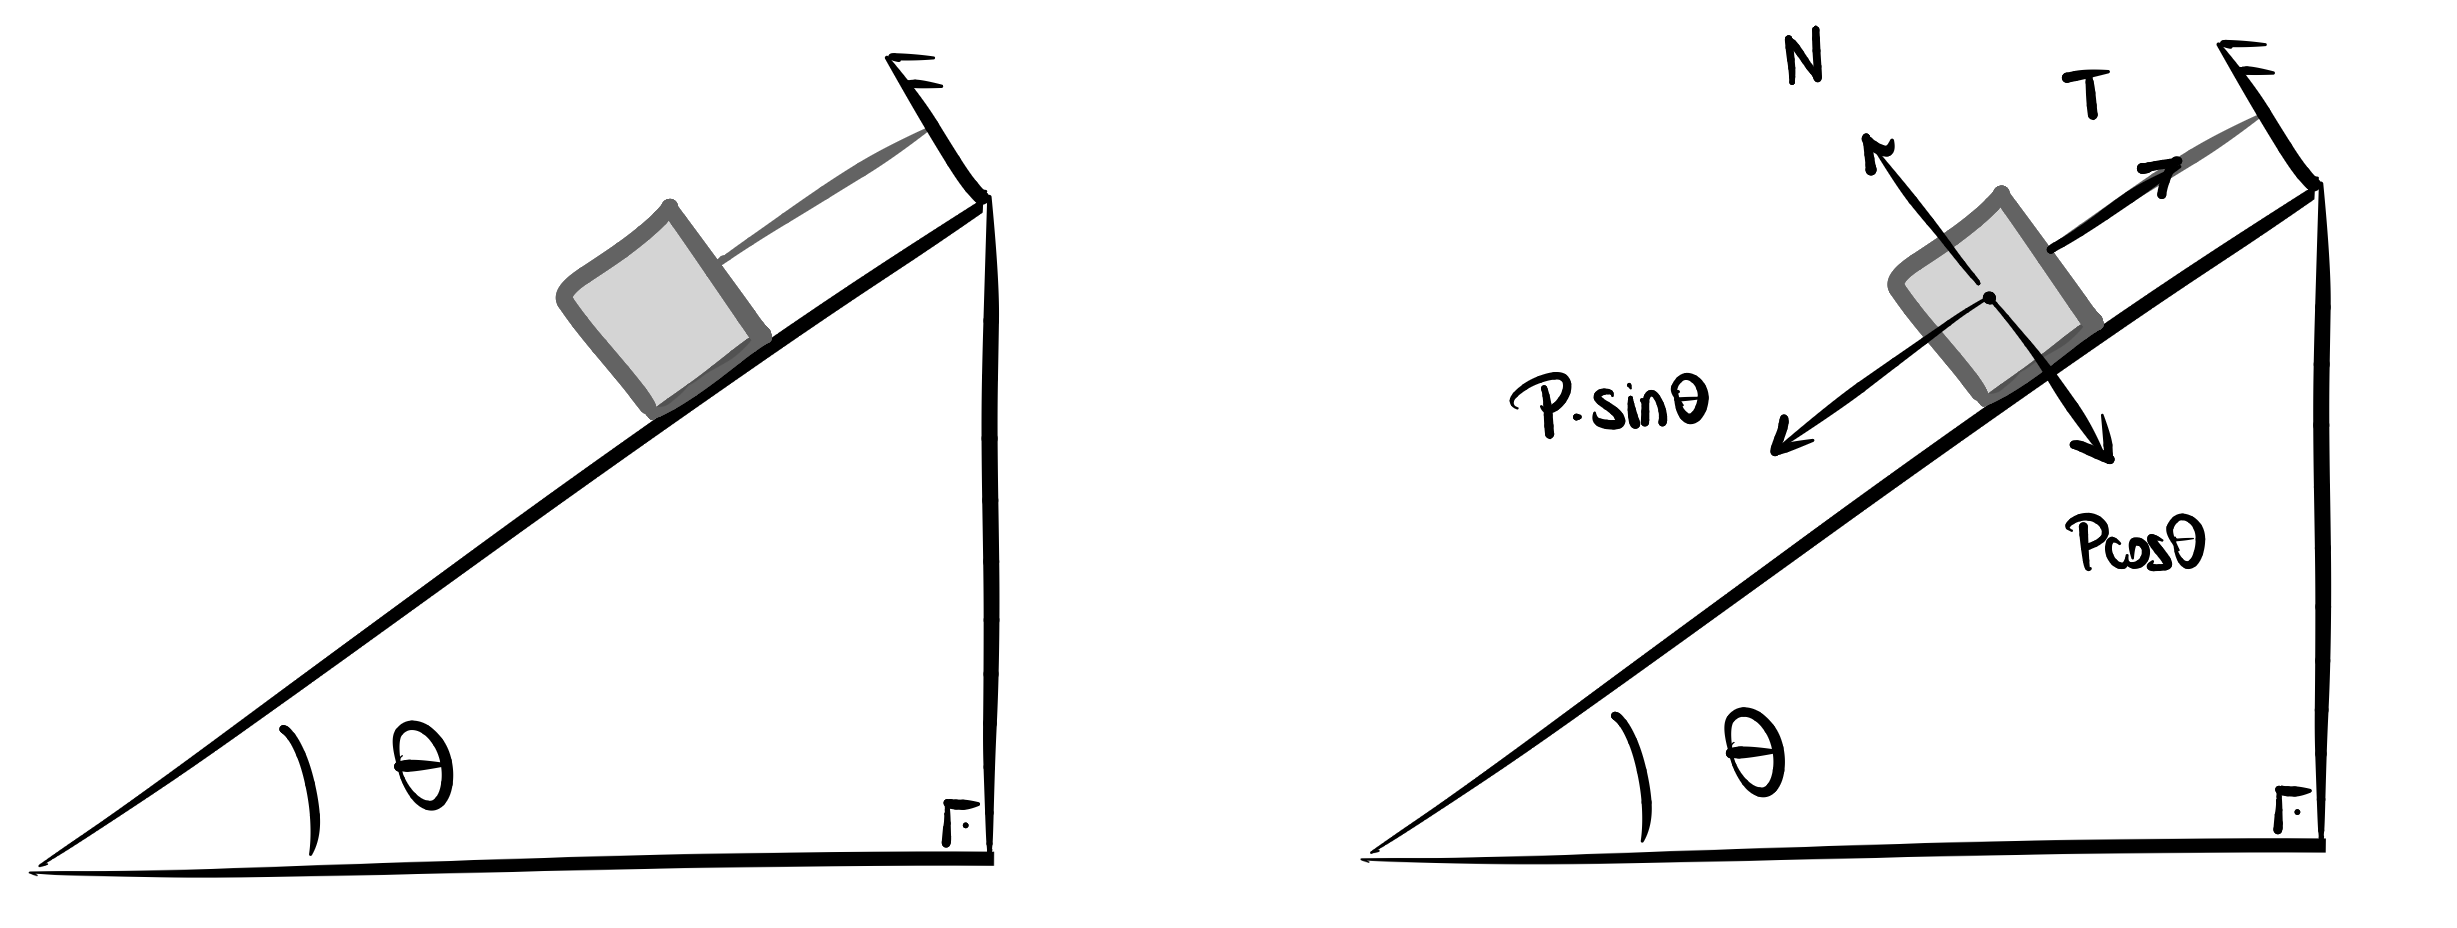
\includegraphics[width=0.6\linewidth]{imagensdinamicanewton/planoinclinadoequilibrio.png}};
  \end{scope}
\end{tikzpicture}
\captionof{figure}{}
\label{fig_newton_planoinclinadoequilibrio}
} 
\vspace{0.3cm}

Do equilíbrio na direção normal tem-se

$$ F_{Ry} = 0 \implies \boxed{N=P\cos \theta ,}$$

\noindent enquanto que o equilíbrio na direção paralela ao plano exige que

$$ F_{Rx} = 0 \implies \boxed{T=P\sin \theta.} $$

Ora, se a máxima tração no fio é de $282$ N, o valor máximo da massa $m$ do bloco para que ele fique em equilíbrio será aquele tal que a equação acima seja satisfeita para o maior valor possível de tração que o fio pode suportar:

$$ T=P\sin \theta \implies 282 = mg \sin (45^\circ) \implies 282 = m \cdot 10 \cdot \dfrac{\sqrt 2}{2} \implies \boxed{m \approx 40 \text{ kg}.}$$


\end{exemplo}


\vspace{0.3cm}
\begin{exemplo}[Nível II]\label{exemplo_newton_equilibrio02}

Considere a situação da Figura \ref{fig_mec_exemploequilibrionivel11}, em que um bloco de massa $m=5$ kg é amarrado por dois fios ideais.

{
\centering
\begin{tikzpicture}
  \begin{scope}[blend mode=multiply]
    \node {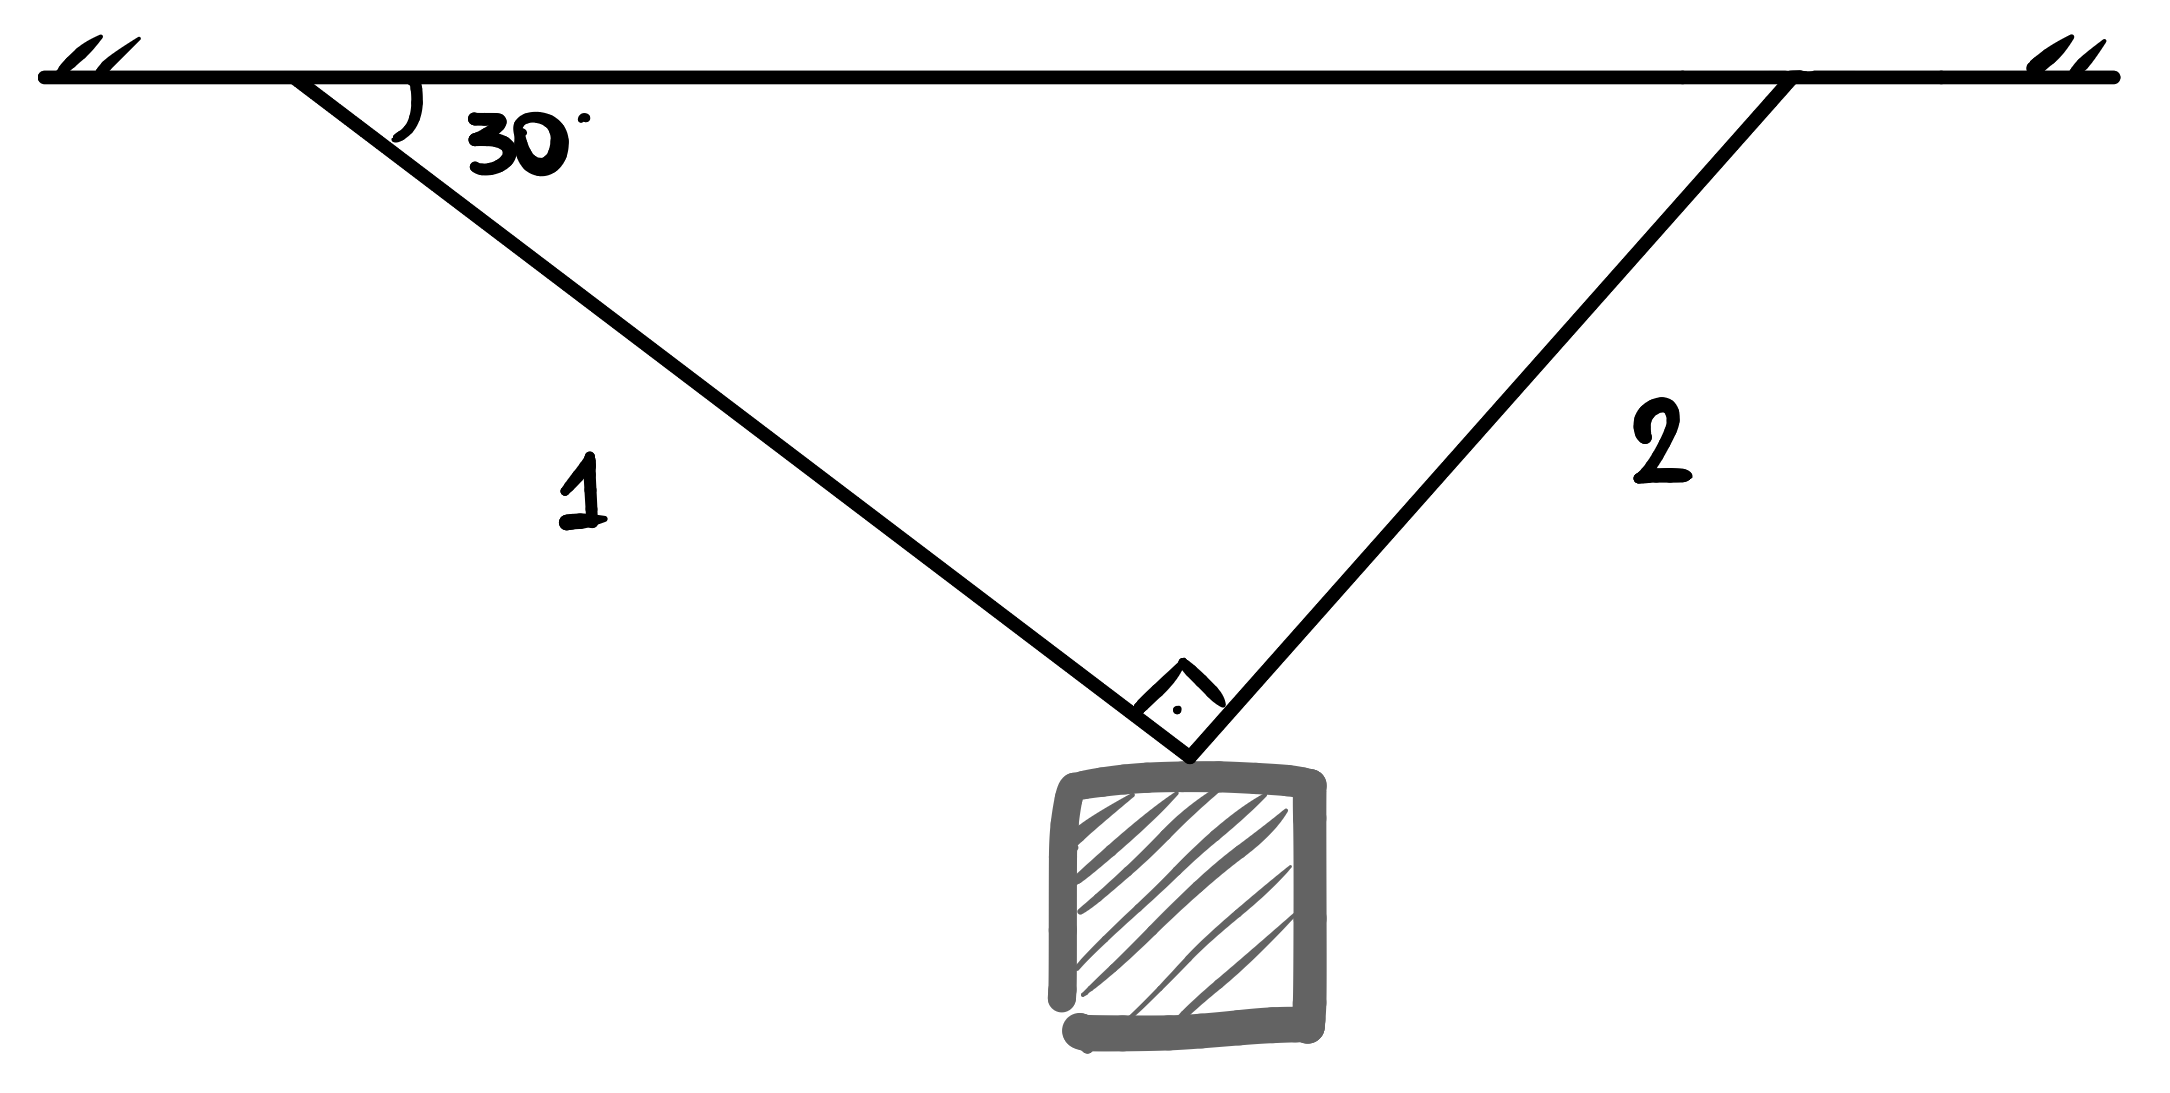
\includegraphics[width=0.4\linewidth]{imagensdinamicanewton/exemploequilibrion11.png}};
  \end{scope}
\end{tikzpicture}
\captionof{figure}{}
\label{fig_mec_exemploequilibrionivel11}
} 
\vspace{0.3cm}

Se o bloco está em equilíbrio, qual é a o valor da maior tração nos fios?

\resolucao

A figura abaixo indica o diagrama de forças que atuam na caixa. 

\vspace{0.3cm}
{
\centering
\begin{tikzpicture}
  \begin{scope}[blend mode=multiply]
    \node {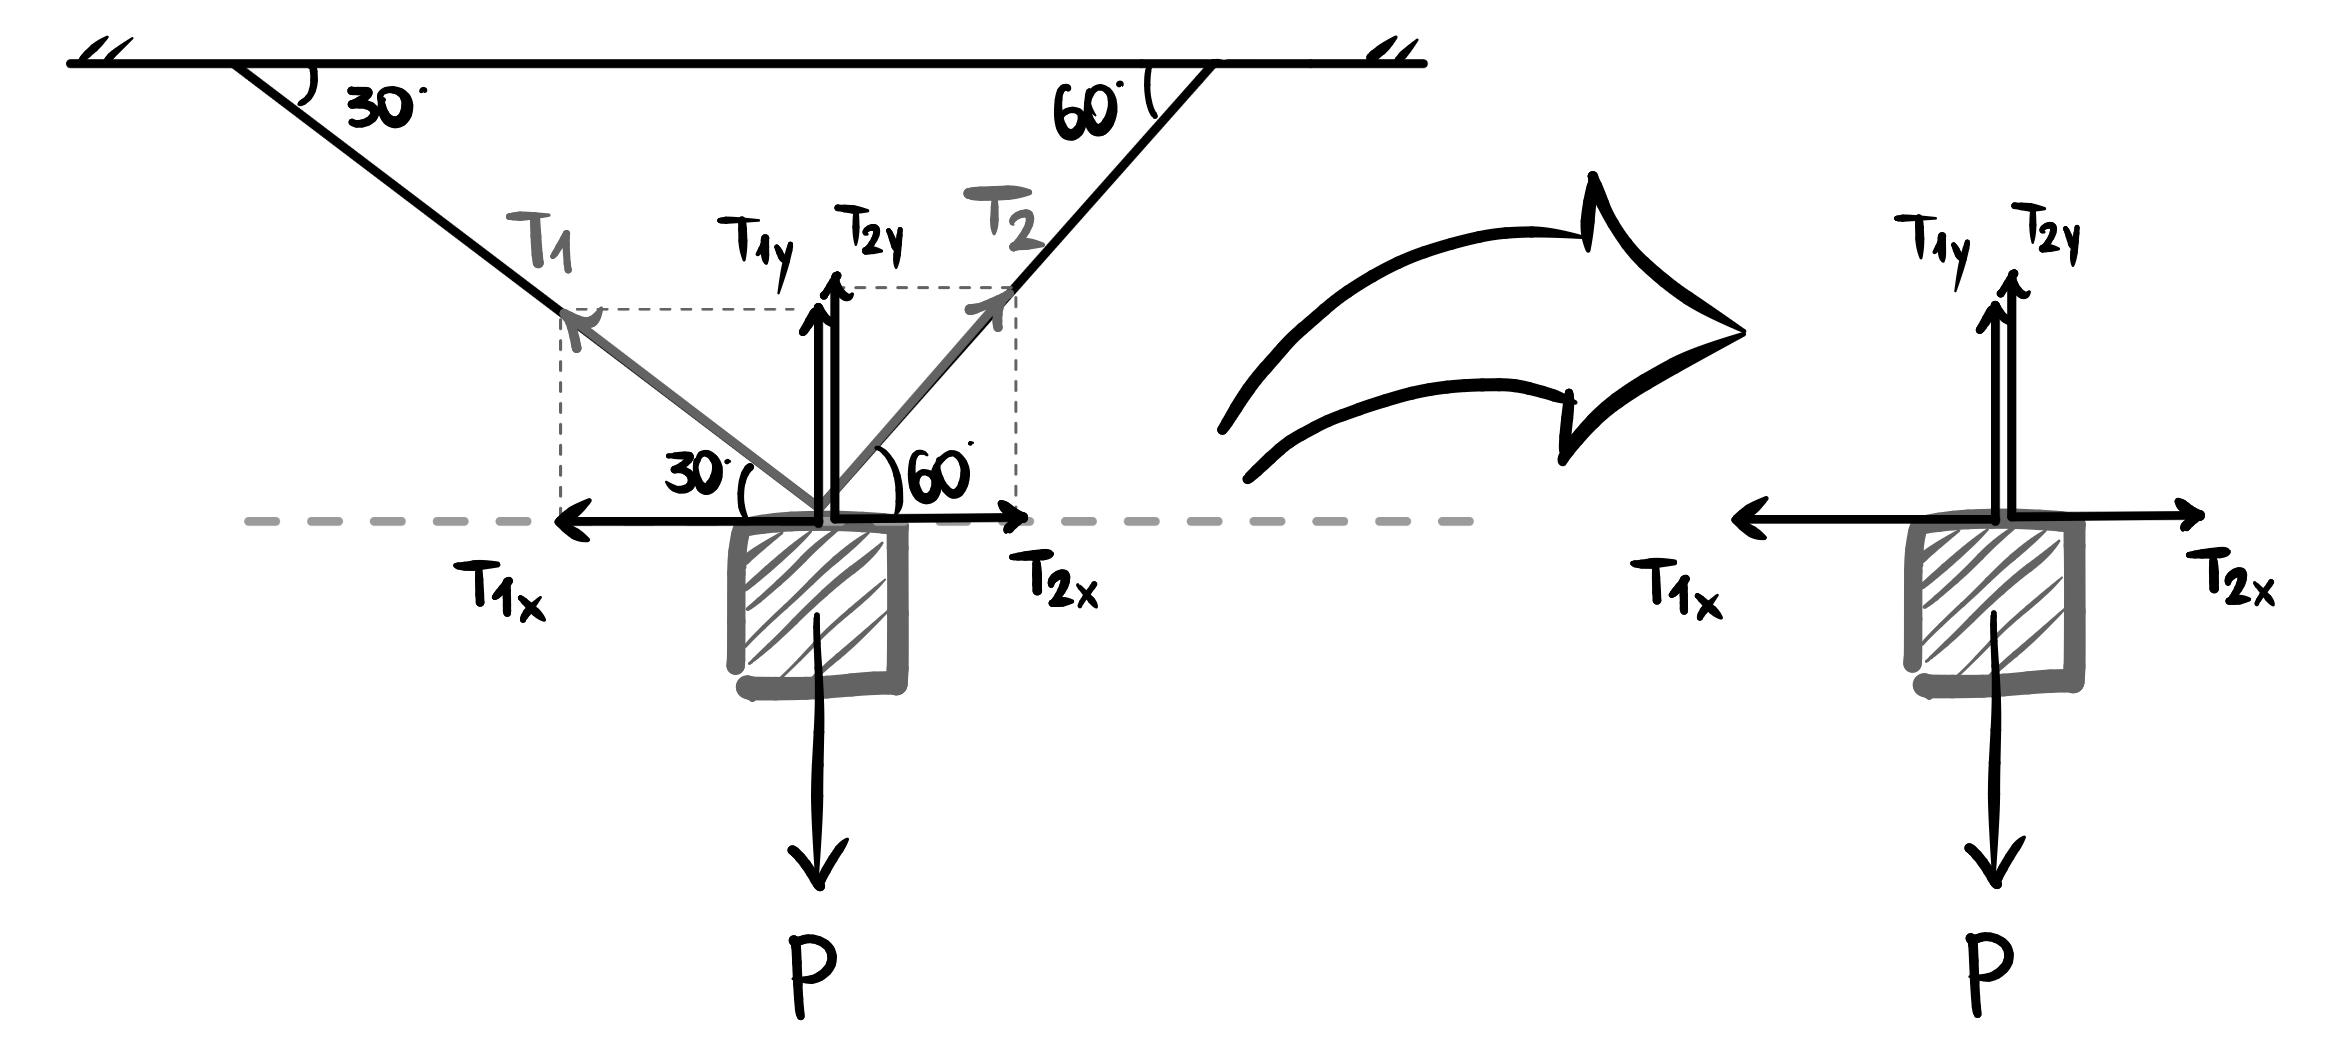
\includegraphics[width=0.7\linewidth]{imagensdinamicanewton/exemploequilibrion12.png}};
  \end{scope}
\end{tikzpicture}
\captionof{figure}{}
\label{fig_mec_exemploequilibrionivel12}
} 
\vspace{0.3cm}

O passo a passo para resolver problemas desse tipo sempre será



\begin{enumerate}
    \item Identificar o corpo cuja dinâmica queremos estudar. No caso, é a caixa.

    \item Desenhar todas as forças que atuam no corpo. Neste caso, trata-se do seu peso, que atua verticalmente para baixo e vale $P=50$N. Além das trações $T_1$ e $T_2$ que atuam nos fios $1$ e $2$, e estão na mesma direção dos fios.

    \item Como queremos impor que $F_R=0,$ daqui em diante podemos agir de duas formas diferentes. A primeira seria escolher um par de eixos perpendiculares nos quais iríamos decompor todas as forças, obrigando-as a serem nulas nas duas direções. 

    Neste caso, escolhemos as direções vertical e horizontal, e, por meio da decomposição vetorial, temos, para o fio 1:

    $$ T_{1x} = T_1 \cos (30) \implies \boxed{T_{1x}=\dfrac{T_1 \sqrt{3}}{2}} \quad \text{e} \quad  T_{1y} = T_1 \sin (30) \implies \boxed{T_{1y}=\dfrac{T_1} {2}.}  $$

    Já para o fio 2 teríamos

     $$ T_{2x} = T_2 \cos (60) \implies \boxed{T_{2x}=\dfrac{T_2}{2}} \quad \text{e} \quad  T_{2y} = T_2 \sin (60) \implies \boxed{T_{2y}=\dfrac{T_2 \sqrt3} {2}.}  $$

     Feito isso, impomos a condição de equilíbrio nas duas direções, isto é, para a direção horizontal teríamos

     $$ F_{Rx} = 0 \implies T_{1x} = T_{2x} \implies  \dfrac{T_1 \sqrt{3}}{2} = \dfrac{T_2}{2} \implies \boxed{T_2=T_1\sqrt 3,}$$

     \noindent e, para a direção vertical, teríamos

     $$ P = T_{1y}+T_{2y} \implies 50 = \dfrac{T_1}{2} + \dfrac{T_2 \sqrt 3}{2} \implies \boxed{T_1 + T_2 \sqrt 3 = 100.}$$

     Usando que $T_2=T_1 \sqrt 3$ na equação acima, somos levados a 

     $$T_1 + (T_1 \sqrt3) \sqrt 3 = 100 \implies T_1 = 25\text{N},$$

     \noindent de modo que a tração no fio 2 é $T_2=T_1 \sqrt 3= 25\sqrt3 \text{N}.$ Logo, a maior tração ocorre no fio 2, e vale $T_2 = 25\sqrt3 \text{N}.$

     
\end{enumerate}

Poderíamos ter procedido de um modo diferente no terceiro passo. Este caminho costuma parecer um pouco mais abstrato no começo, porque exige um maior manejo geométrico. Mas, como veremos, os cálculos se tornarão bem mais simples. \\

Neste caso, ao invés de decompor as forças para falar que elas se anulam em $x$ e em $y$, escreveremos uma única equação vetorial de equilíbrio: 


\[
 \vec{F}_R = 0
\quad \xrightarrow{\text{projeção nos eixos}}
\quad
\begin{cases}
F_x = 0 \\
F_y = 0
\end{cases}
\]

Ou seja, ao invés de projetarmos nos eixos e escrevermos duas equações de equilíbrio, escreveremos uma única equação, porém elas será vetorial -- e, por isso, exigirá uma interpretação geométrica. Impondo que $\vec{F}_R=0,$ teremos

$$\vec{T}_1+\vec{T}_2+\vec{P}=0.$$

É importante que o leitor perceba que a equação acima é vetorial: ela leva em consideração o vetor $\vec{T_1},$ com sua direção e sentido. Enquanto que a equação que envolve $T_{1x}$ não é vetorial, mas escalar: ela envolve o valor de uma projeção do vetor $\vec T_1$ -- o tamanho da sua projeção horizontal.

Tal equação pode ser reescrita como 

$$\vec{T}_1+\vec{T}_2+\vec{P}=0 \implies \vec{T}_1+\vec{T}_2 = -\vec{P} ,$$

\noindent ou seja, os vetores $\vec T_1 \text{ e } \vec T_2$ somados devem resultar no oposto do vetor peso. A Figura \ref{fig_mec_exemploequilibrioexemplofios} ilustra essa situação. 


\vspace{0.3cm}
{
\centering
\begin{tikzpicture}
  \begin{scope}[blend mode=multiply]
    \node {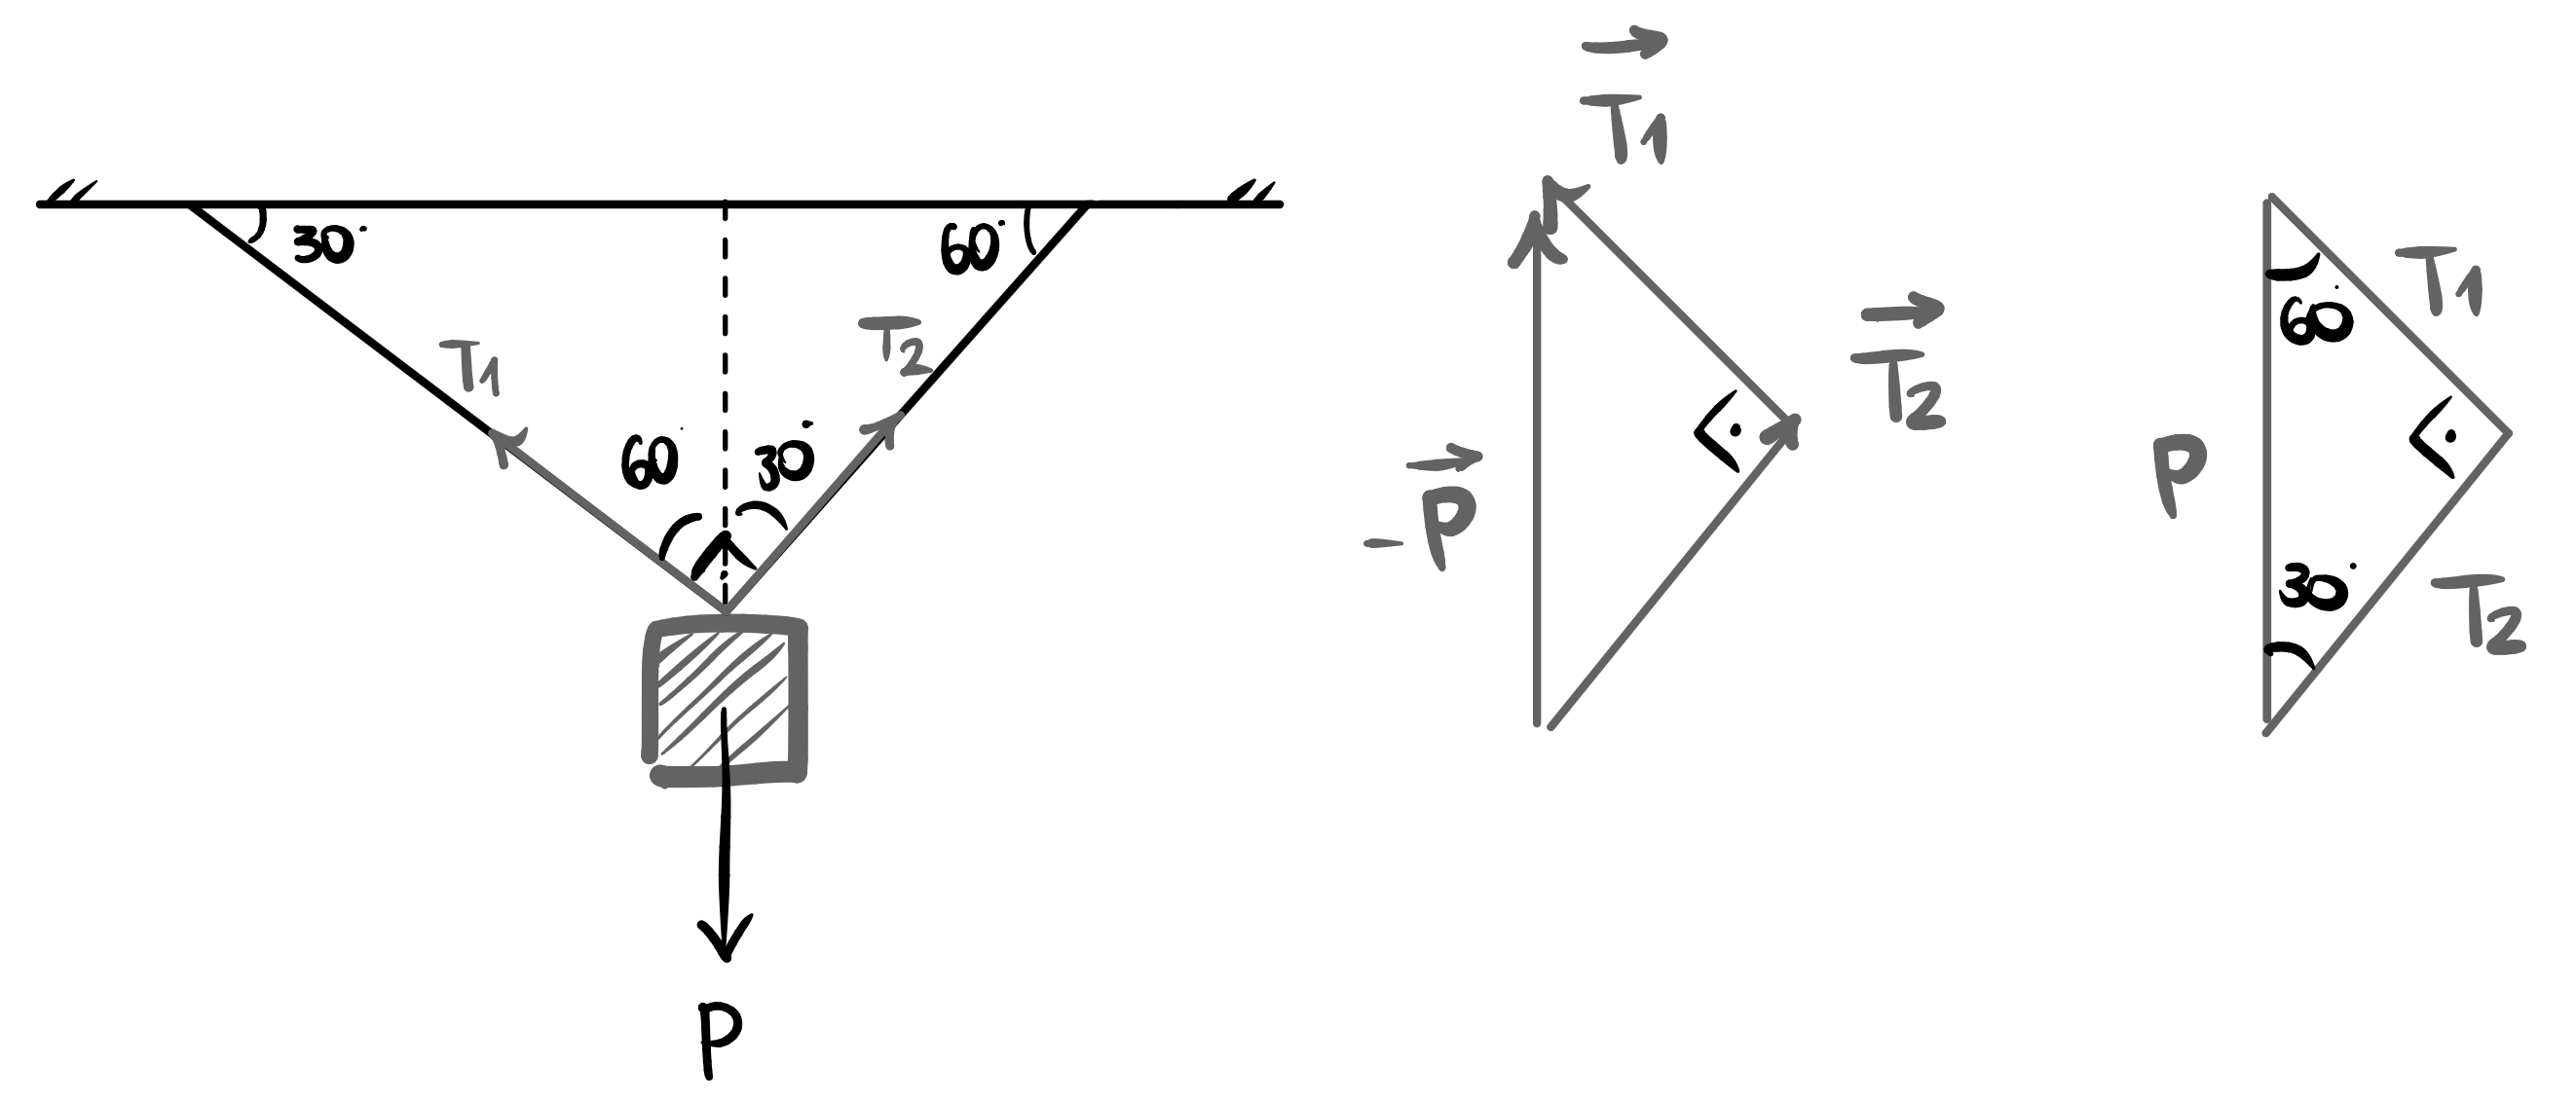
\includegraphics[width=0.7\linewidth]{imagensdinamicanewton/equilibrio exemplo fios.png}};
  \end{scope}
\end{tikzpicture}
\captionof{figure}{}
\label{fig_mec_exemploequilibrioexemplofios}
} 
\vspace{0.3cm}



Como vemos, na primeira imagem, optamos por não decompor os vetores. A imagem do meio mostra, geometricamente, o que significa a equação vetorial $ \vec{T}_1+\vec{T}_2 = -\vec{P},$ enquanto que a última imagem desconsidera o seu caráter vetorial (para onde as setas apontam) e mantém apenas suas características geométricas: tem-se um triângulo, retângulo (haja vista que os fios eram perpendiculares) de lados cujos tamanhos medem $P,$ $T_1$ e $T_2.$ \\

A primeira imagem da figura já indica que o ângulo entre o fio 1 e a vertical (direção do peso) é igual a $60^\circ$, enquanto que o ângulo entre o fio 2 e a vertical (direção do peso) é de $30^\circ$. Tais informações estão no triângulo da última figura, nos ângulos entre as direções de $T_1$ e $T_2$ com a vertical (direção do peso). \\

Note que, até então, ainda não fizemos nenhum cálculo, apenas uma construção geométrica. Munidos dela, podemos obter as trações diretamente, com um único cálculo, usando a definição das razões trigonométricas no triângulo retângulo. Para o caso de $T_2,$ teríamos

$$ \sin(60^\circ) = \dfrac{T_2}{P} \implies T_2 = P \sin(60^\circ) = 50 \cdot \dfrac{\sqrt 3}{2} \implies \boxed{T_2 =25 \sqrt 3 \text{N}.} $$

Perceba que este segundo caminho torna o cálculo algébrico muito simples, por trocar duas equações (equilíbrio em $x$ e em $y)$ por uma única. O preço a se pagar é que a equação de equilíbrio vetorial precisa ser interpretada geometricamente. Isso, contudo, sempre vai ocorrer: se um corpo está em equilíbrio sobre a ação de um certo número de forças, então tais forças irão formar um polígono fechado. No caso de 3 forças, trata-se de um triângulo. Se fossem 4 ou 6 teríamos um quadrilátero e um hexágono, respectivamente. Tais figuras nos permitirão escrever, geometricamente, a equação de equilíbrio $\vec F_R =0.$



\end{exemplo}



\vspace{0.3cm}



\begin{exemplo}[Nível III]\label{exemplo_newton_equilibrio03}

Considere a generalização do exemplo anterior: um bloco de massa $m$ está preso por dois fios, que fazem os ângulos $\theta$ e $\phi$ com a parede do teto, como mostra a Figura \ref{fig_mec_leisnewtonequilibrioexemplonivel31}.


\vspace{0.3cm}
{
\centering
\begin{tikzpicture}
  \begin{scope}[blend mode=multiply]
    \node {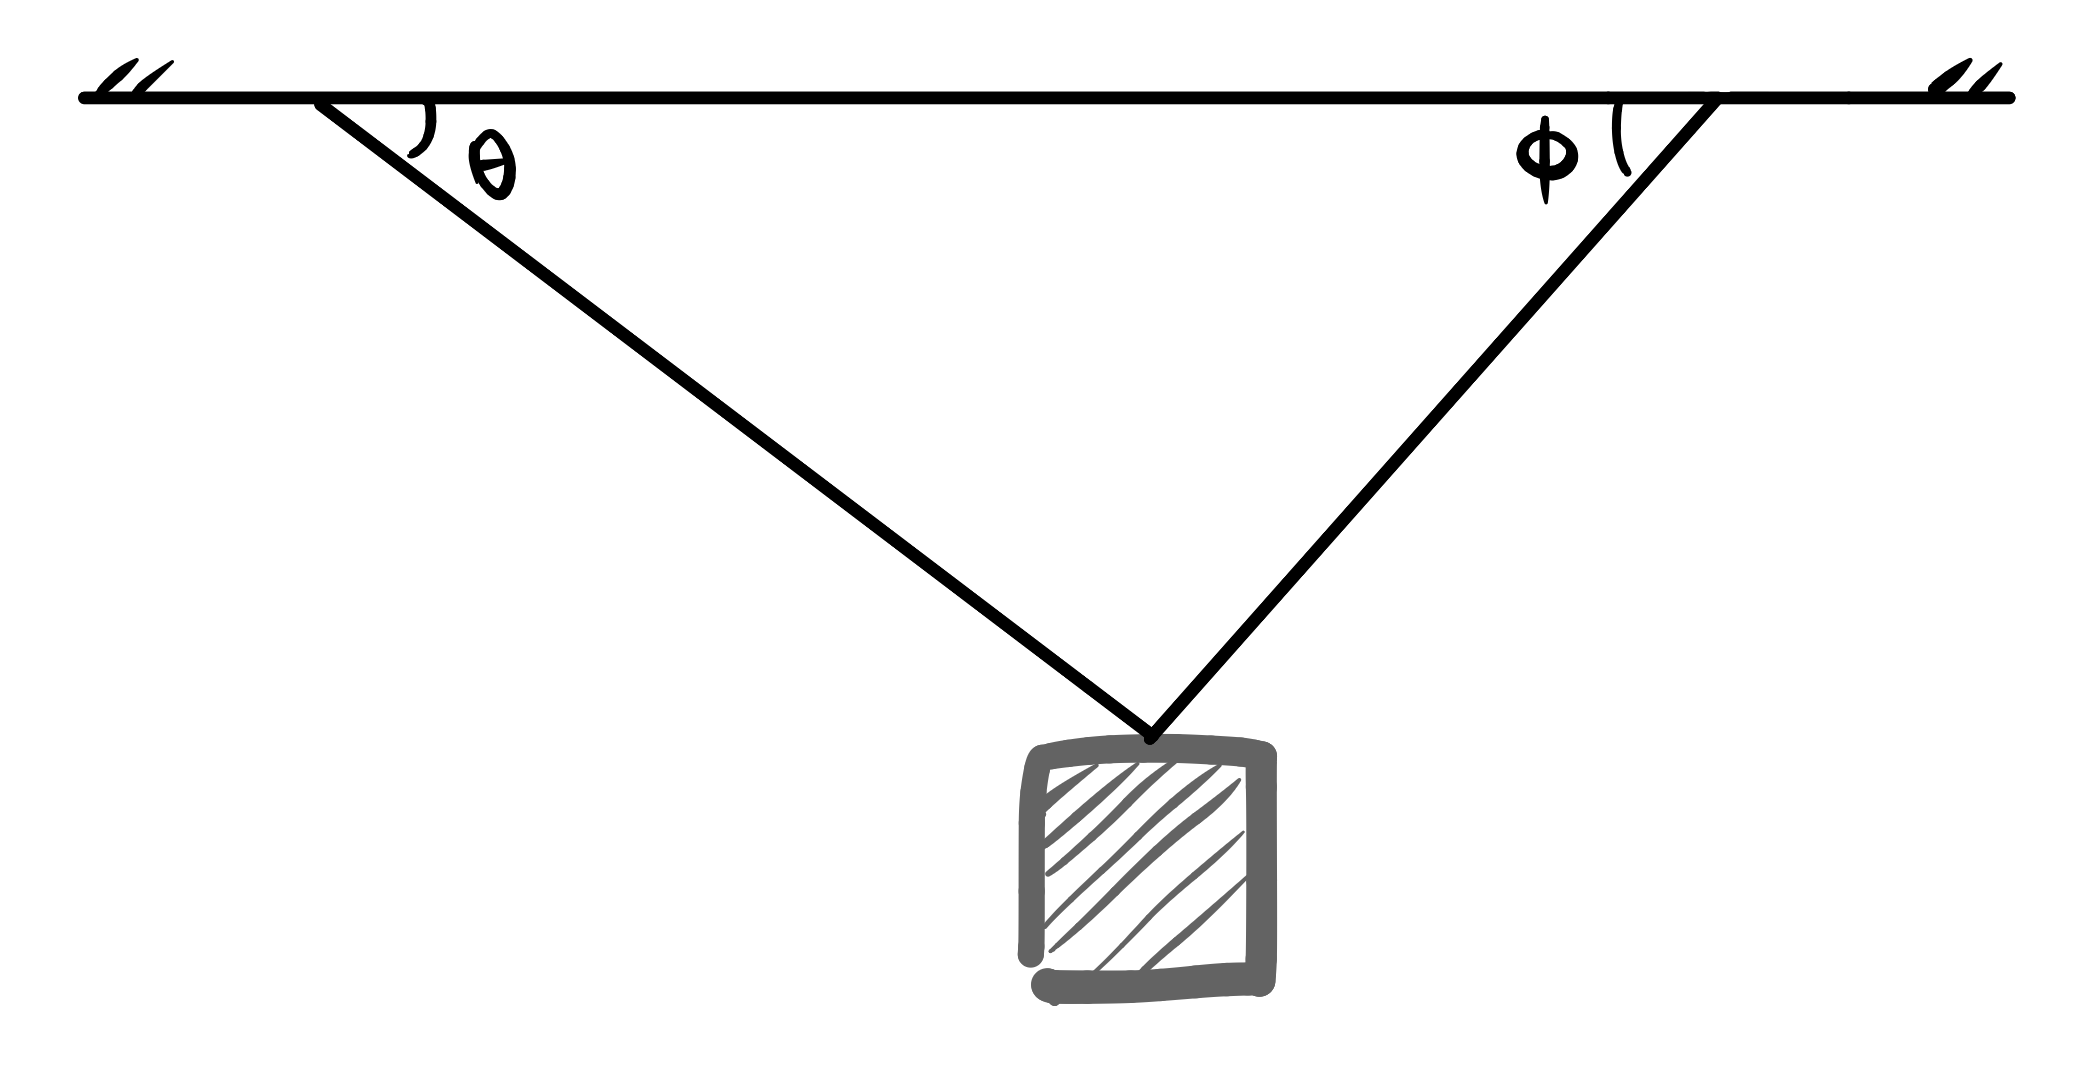
\includegraphics[width=0.4\linewidth]{imagensdinamicanewton/leisnewtonequilibrioexemplonivel31.png}};
  \end{scope}
\end{tikzpicture}
\captionof{figure}{}
\label{fig_mec_leisnewtonequilibrioexemplonivel31}
} 
\vspace{0.3cm}


Encontre a razão entre as trações nos fios quando o bloco está em repouso.

\resolucao

A Figura \ref{fig_mec_leisnewtonequilibrioexemplonivel32} ilustra o diagrama de forças na caixa. Tomando o segundo caminho do exemplo anterior, escreveremos uma única equação de equilíbrio, a equação vetorial:

$$ \vec F_R = \vec T_1 + \vec T_2 + \vec P = 0 \implies \vec T_1 + \vec T_2 = - \vec P.$$

Ou seja, os vetores $\vec T_1 $ e $\vec T_2 $ somados devem dar um vetor vertical, apontando para cima, do mesmo tamanho do vetor peso. Tal situação está representada no triângulo no desenho da direita da Figura \ref{fig_mec_leisnewtonequilibrioexemplonivel32}.

\vspace{0.3cm}
{
\centering
\begin{tikzpicture}
  \begin{scope}[blend mode=multiply]
    \node {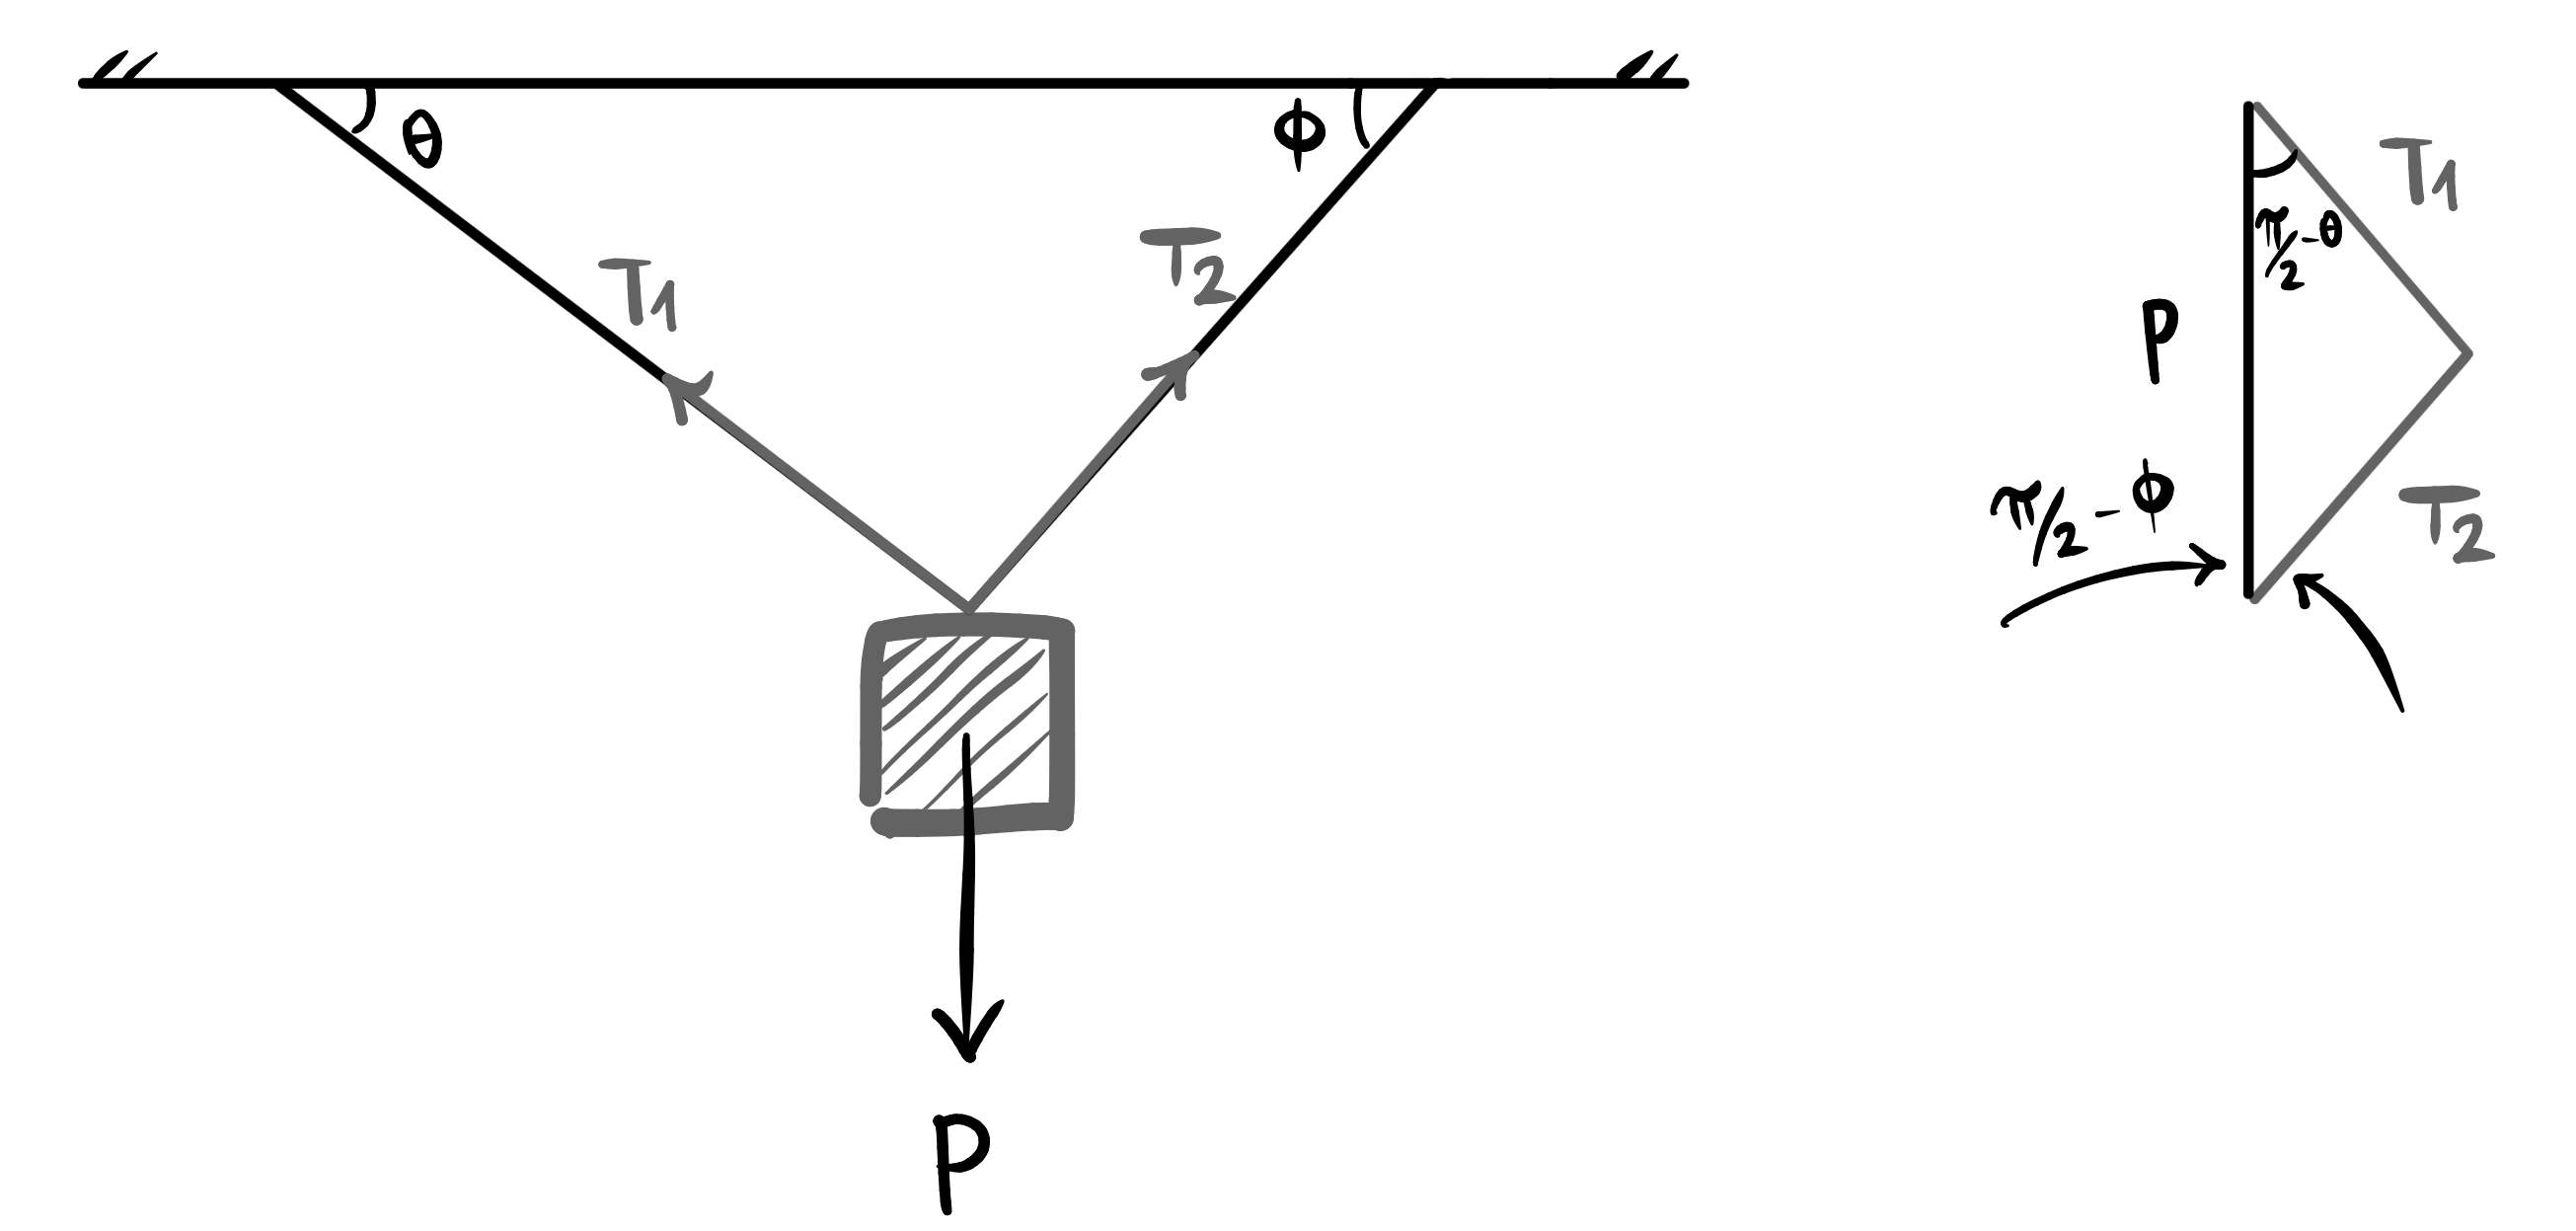
\includegraphics[width=0.7\linewidth]{imagensdinamicanewton/leisnewtonequilibrioexemplonivel32.png}};
  \end{scope}
\end{tikzpicture}
\captionof{figure}{}
\label{fig_mec_leisnewtonequilibrioexemplonivel32}
} 
\vspace{0.3cm}

Da imagem da esquerda de tal figura, ao traçar uma vertical passando pelo centro da caixa, obtém-se facilmente os ângulos entre os fios e a vertical, que aparecem representados já no triângulo da figura da direita. Pela Lei dos Senos em tal triângulo podemos escrever que

$$ \dfrac{T_2}{\sin \left( \dfrac{\pi}{2} - \theta \right)} = \dfrac{T_1}{\sin \left( \dfrac{\pi}{2} - \phi \right)} = \dfrac{P}{\sin \left(\phi +\theta \right)}.$$

Da primeira igualdade extraímos

$$ \boxed{\dfrac{T_2}{T_1} = \dfrac{\cos \theta}{\cos \phi}.}$$



\end{exemplo}









\begin{secnivel}[Força na Polia Fixa]{I}{Força na Polia Fixa}
  
  \eqLdois{dem}{eq_newton_poliafixa}{F_\text{FINAL}=F}

\end{secnivel}


 A força $F$ em tal equação representa a força feita por um indivíduo na extremidade uma corda que passa por uma polia (roldana) fixa, como mostra Figura \ref{fig_dinamicanewton_poliafixa01}. A força $F_\text{FINAL}$ que chega em uma extremidade da corda é igual à força $F$ feita na outra extremidade.

A Equação \eqref{eq_newton_poliafixa}, portanto, constata que a força transmitida ao longo do fio é a mesma.




\secgfe{De onde vem}

Uma polia -- ou roldana -- fixa é aquela que está, como o próprio nome indica, presa em alguma parede ou anteparo. Sendo assim, ela está fixa e não tem nenhuma liberdade de se mover. Em polias fixas ideais\footnote{Sempre trabalharemos com polias ideias -- aquelas de massa desprezível -- no contexto do Ensino Médio. Do contrário, sua inércia de rotação teria que ser levada em conta, o que exigiria cálculos mais avançados do que as ferramentas do ensino médio possibilitam fazer.} o seu uso será apenas o de mudar a direção em que se aplica a força, como mostra a Figura \ref{fig_dinamicanewton_poliafixa01}.

Perceba, em tal figura, que para sustentar parado, digamos, um bloco de peso $P=200$N, a força necessária a ser feita deverá ser exatamente igual a $200$N. O indivíduo pode puxar a corda em diferentes direções, mas sempre terá que fazer uma força exatamente igual ao peso do bloco para mantê-lo parado. A roldana fixa, portanto, é um dispositivo que não aumenta o diminui a força feita em uma extremidade -- a força se transmite integralmente até a outra extremidade do fio.

A utilidade de um dispositivo como esse, portanto, não é puxar um bloco fazendo menos força do que o valor de seu peso, mas apenas o de facilitar a execução de tal força por fazê-la através de uma corda.

\vspace{0.3cm}
{
\centering
\begin{tikzpicture}
  \begin{scope}[blend mode=multiply]
    \node {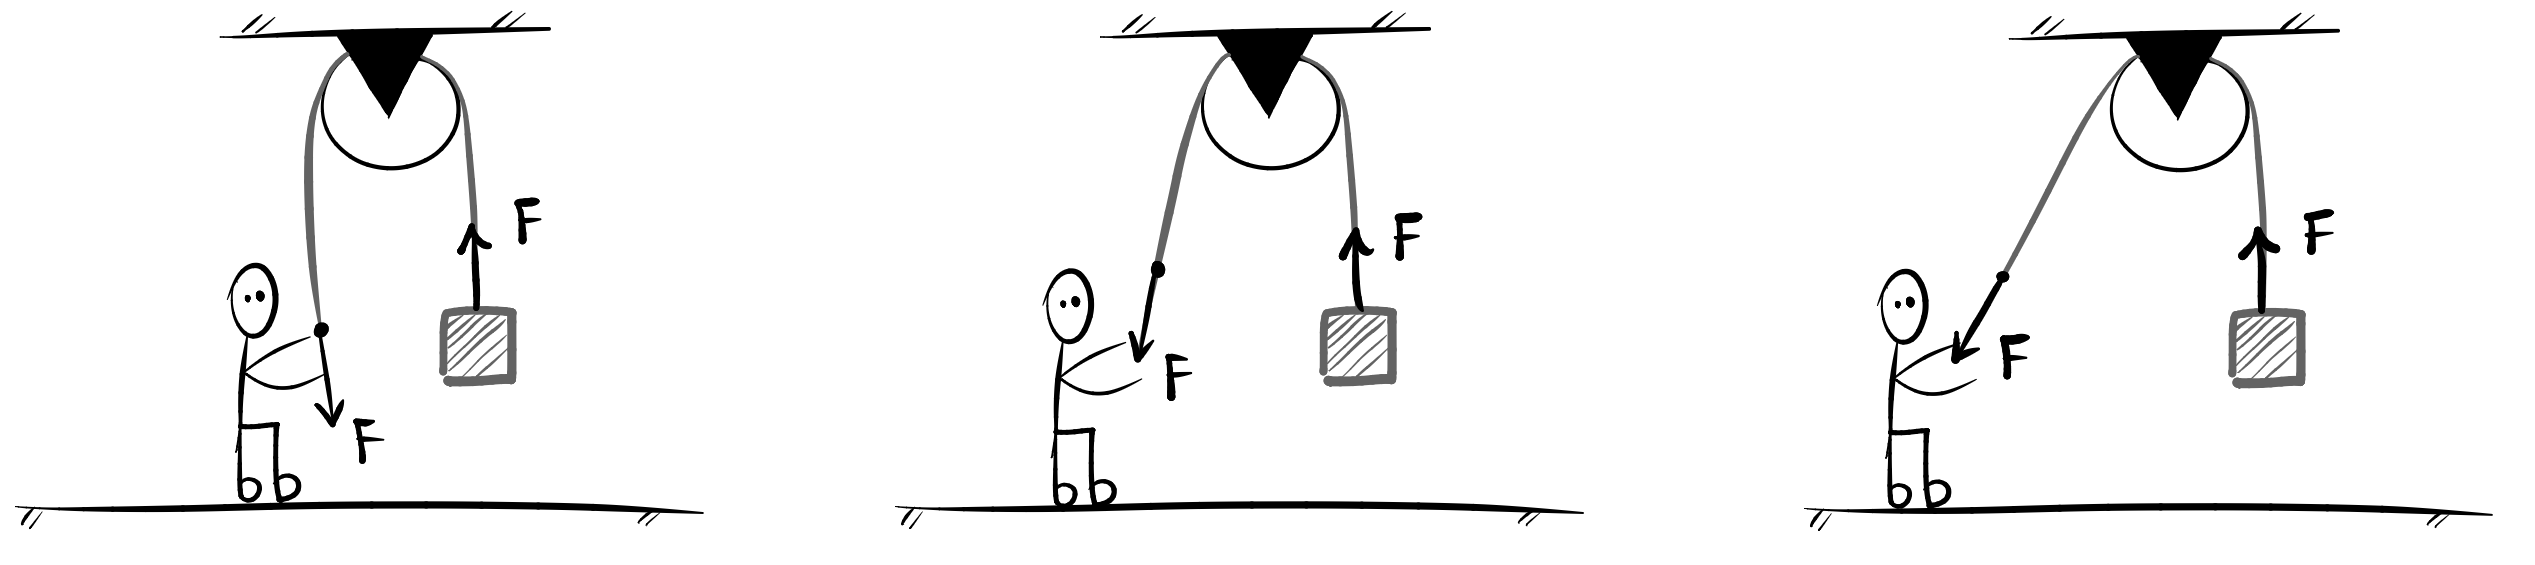
\includegraphics[width=0.9\linewidth]{imagensdinamicanewton/poliafixa01.png}};
  \end{scope}
\end{tikzpicture}
\captionof{figure}{O funcionamento de uma polia fixa.}
\label{fig_dinamicanewton_poliafixa01}
} 
\vspace{0.3cm}

No desenvolvimento da Equação \eqref{eq_newton_terceiraleinewton} nós exploramos o conceito de tração em um fio e a definição de um fio ideal. Ali nós provamos, matematicamente, que ao longo de um fio ideal a tração é sempre a mesma. Como o sistema de uma roldana fixa consiste em um disco fixado e um fio ideal que passa através dele, é de se esperar que a força (tração) ao longo do fio seja sempre a mesma, como provamos na discussão sobre a Terceira Lei de Newton. É exatamente isso que a Equação \eqref{eq_newton_poliafixa} diz.

\secgfe{Onde é usada}

Polias aparecem em diversos contextos nos quais deseja-se, em geral, carregar um objeto pesado. Diversos aparelhos de academias possuem polias, para mudar a direção com que se aplica certas forças ao carregar um mesmo peso, a fim de trabalhar músculos diferentes, por exemplo.

Imagine a dificuldade em carregar um objeto grande e pesado, como, digamos, um piano. É muito mais fácil amarrá-lo por uma corda e puxá-lo por essa corda, em um sistema como o da Figura \ref{fig_dinamicanewton_poliafixa01}. Por mais que a força exercida na corda deva ser pelo menos igual ao peso do piano para levantá-lo, será muito mais simples executar tal força ao longo de uma corda -- o que pode inclusive ser realizado por uma máquina, como no funcionamento de um elevador -- do que carregar o piano diretamente. 

\secgfe{Erros comuns}

Os erros mais comuns aqui consistem em confundir a polia fixa com a polia móvel, que será estudada na próxima seção. 

Além disso é comum o estudante acreditar que a força necessária para carregar um objeto na situação da Figura \ref{eq_newton_poliafixa} irá depender do ângulo da corda. Tal figura, contudo, já mostra que isso está equivocado: a força que se propaga no fio é sempre a mesma feita na outra extremidade, independente da direção do fio.


\secgfe{Observações}

Costuma-se dizer que a polia fixa é um sistema que não oferece vantagem mecânica, isto é, a força que se faz é exatamente a mesma que chega na outra extremidade. Um dispositivo que oferece vantagem mecânica seria aquele que multiplica essa força ao longo do seu caminho, como a própria polia móvel o faz, como veremos.

Contudo, embora a polia fixa não reduza a intensidade da força necessária para erguer um corpo -- já que, no modelo ideal, a tração no fio é igual ao peso da carga -- ela pode tornar o esforço humano significativamente mais confortável e eficiente do ponto de vista biomecânico. Ao permitir que a pessoa puxe o fio para baixo em vez de levantar o peso para cima, a polia transforma a ação em algo mais natural: é mais fácil aplicar força no sentido descendente, aproveitando o próprio peso do corpo e recrutando grupos musculares mais fortes, como os dorsais e os bíceps, em vez de depender apenas dos ombros. Além disso, puxar para baixo melhora o equilíbrio e o controle do movimento, reduzindo a instabilidade. 

Assim, a polia fixa não oferece vantagem mecânica em termos físicos -- não há redução da força exigida --, mas oferece uma vantagem operacional e ergonômica que explica por que ela é tão útil na prática e porque, mesmo fazendo a mesma força, o esforço necessário para carregar o mesmo objeto pareça menor usando um sistema de polia fixa.


\vspace{0.3cm}


\begin{exemplo}[Nível I]\label{exemplo_newton_poliafixa01}

Considere a situação da Figura \ref{fig_mec_poliafixaex1} em que o ângulo do plano inclinado é $\theta = 30^\circ$ e a massa do bloco é $m=10$ kg. Se o bloco sobe com velocidade constante, qual é a força feita pelo menino?

{
\centering
\begin{tikzpicture}
  \begin{scope}[blend mode=multiply]
    \node {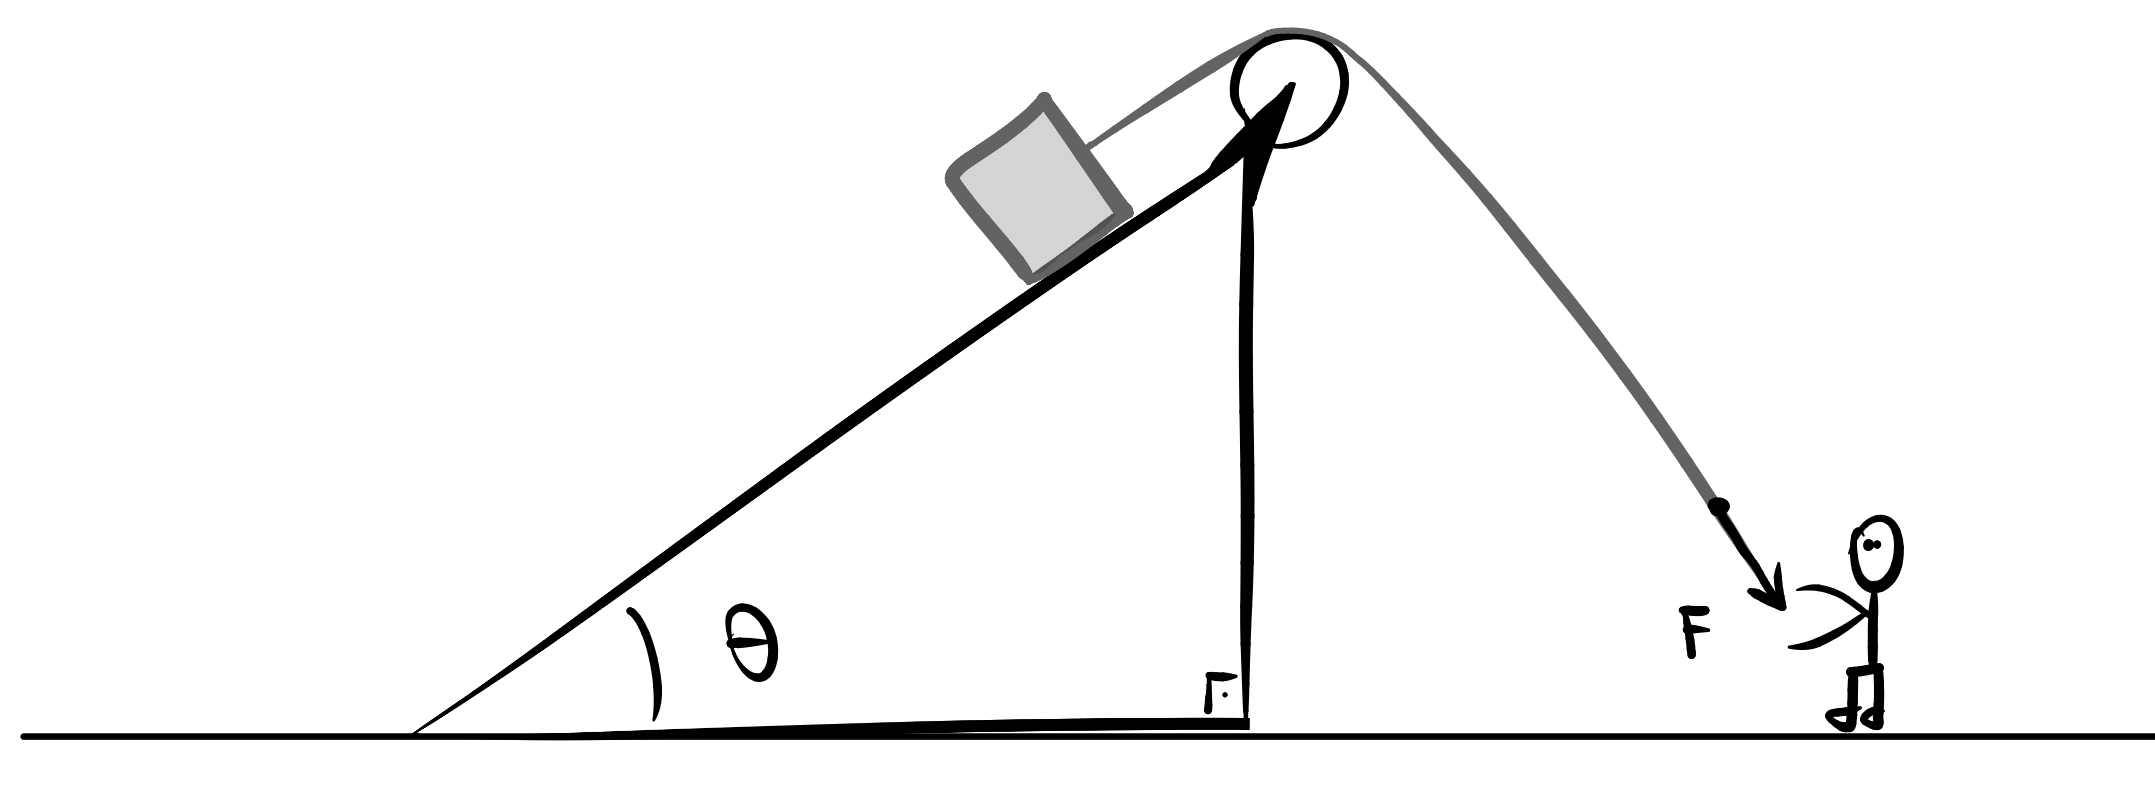
\includegraphics[width=0.5\linewidth]{imagensdinamicanewton/poliafixa1.png}};
  \end{scope}
\end{tikzpicture}
\captionof{figure}{}
\label{fig_mec_poliafixaex1}
} 


\resolucao

Se o bloco sobe com velocidade constante (MRU) isso significa que ele está em equilíbrio dinâmico, ou seja, $F_R =0.$ Analisando as forças na direção do plano inclinado teremos a tração puxando o bloco plano acima e a componente $P \sin \theta$ do peso puxando o bloco plano abaixo (veja o desenvolvimento da Equação \eqref{eq_dinamicanewtoniana_gsintheta} em caso de surpresa com tal expressão). Sendo assim, equacionado o equilíbrio em tal direção teremos

$$ T = P \sin \theta = mg \sin 30^\circ = 10 \cdot 10 \cdot \dfrac{1}{2} \implies T = 50 \text{ N.}$$

Como trata-se de um sistema de polia fixa, a força feita pelo menino em uma extremidade do fio é exatamente aquela que se propaga e chega na outra extremidade. Logo, o menino faz uma força $F$ tal que 

$$ \boxed{F=T=50 \text{ N.}}$$



\end{exemplo}

\vspace{0.3cm}




\begin{exemplo}[Nível II (Escola Naval - 2019)]\label{exemplo_newton_poliafixa02}

Analise a figura abaixo.


{
\centering
\begin{tikzpicture}
  \begin{scope}[blend mode=multiply]
    \node {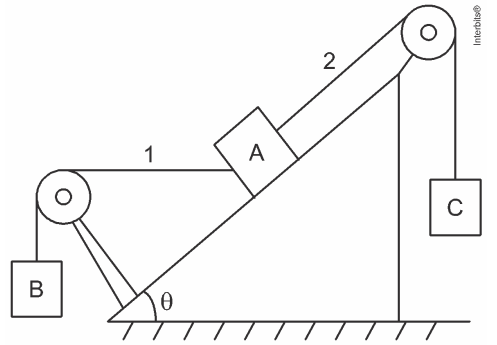
\includegraphics[width=0.4\linewidth]{imagensdinamicanewton/poliafixa2.png}};
  \end{scope}
\end{tikzpicture}
\captionof{figure}{}
\label{fig_mec_poliafixaex2}
} 


A figura representa o perfil de um plano inclinado de um ângulo $\theta$ no qual estão fixas duas polias ideais, de modo que o trecho do fio 1 é horizontal e o trecho do fio 2 é paralelo ao plano inclinado. Os fios são ideais e os atritos são desprezíveis. Sabendo-se que os blocos $A$ e $B$ têm o mesmo peso $P$, qual deve ser o peso do bloco $C$ para que o sistema permaneça em equilíbrio?

\begin{enumerate}
    \item [a)] $P(\sin\theta+\cos\theta)$
    \item [b)]$P(\sin\theta-\cos\theta)$
    \item [c)]$2P\sin\theta$
    \item [d)]$2P\cos\theta$
    \item [e)]$\dfrac{P}{2}\,(\sin\theta+\cos\theta)$
\end{enumerate}


\resolucao

A Figura \ref{fig_mec_newetonpoliafixaexmplonivel2} ilustra a situação com o diagrama de todas as forças que atuam nos blocos. Começando pela direita, a tração $T_1$ no primeiro fio deve ser igual ao peso $P_C$ do bloco $C$, isto é: $T_1 = P_C$.

\vspace{0.3cm}
{
\centering
\begin{tikzpicture}
  \begin{scope}[blend mode=multiply]
    \node {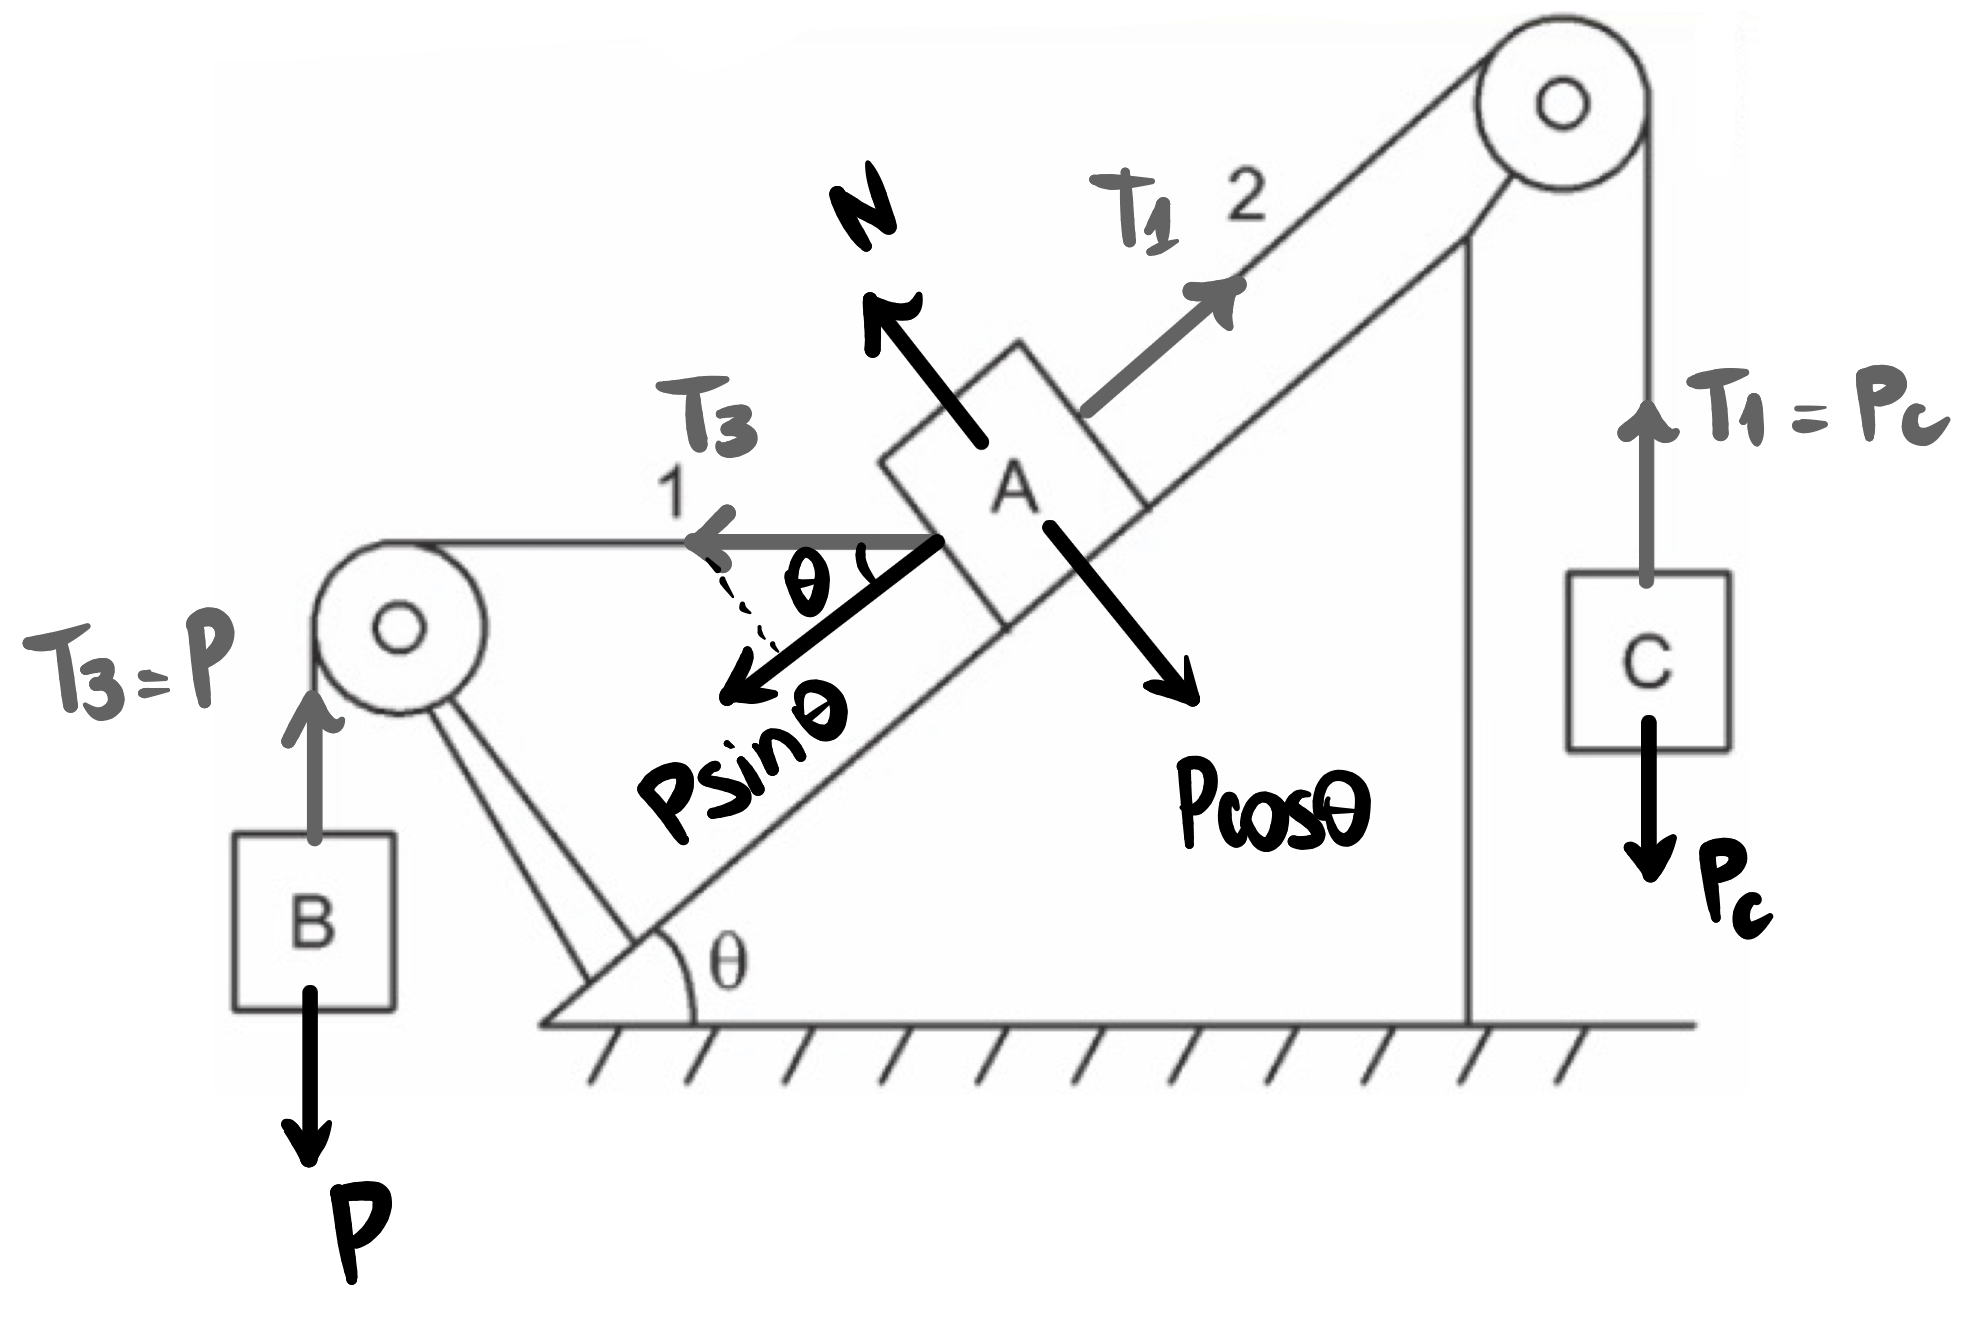
\includegraphics[width=0.45\linewidth]{imagensdinamicanewton/newetonpoliafixaexmplonivel2.png}};
  \end{scope}
\end{tikzpicture}
\captionof{figure}{}
\label{fig_mec_newetonpoliafixaexmplonivel2}
} 
\vspace{0.3cm}

Essa tração se propaga, puxando o bloco $A$ na direção plano acima. Do lado esquerdo, a tração $T_3$ no fio vertical deve ser igual ao peso $P$ do bloco $B$, ou seja, $T_3 = P.$ Essa tração se propaga, puxando horizontalmente o bloco $A.$  

Já no bloco $A$, representamos a normal $N$ feita pelo plano sob ele e a sua força peso $P$, já decomposta nas componentes paralela ao plano, $P \sin \theta$, e perpendicular ao plano, $P \cos \theta.$ Equacionando o equilíbrio das forças na direção do plano será necessário decompor a tração $T_3,$ que possui componente $T_3 \cos \theta$ na direção do plano. Logo, em tal direção, aplicando $F_\text{R} = 0,$ somos levados a

$$ P \sin \theta + T_3 \cos \theta = T_1,$$

\noindent e, como $T_3 = P$ e $T_1 = P_C$, segue que 

$$ \boxed{ P_C = P \sin \theta + P \cos \theta \implies \text{letra A}.}$$

\end{exemplo}

\vspace{0.3cm}





\begin{exemplo}[Nível III (ITA 1996)]  \label{exemplo_newton_poliamovel03}

Dois blocos de massa $M$ estão unidos por um fio de massa desprezível que passa por uma roldana com eixo fixo. 
Um terceiro bloco de massa $m$ é colocado suavemente sobre um dos blocos, como mostra a figura. 
Com que força esse pequeno bloco de massa $m$ pressionará o bloco sobre o qual foi colocado?

{
\centering
\begin{tikzpicture}
  \begin{scope}[blend mode=multiply]
    \node {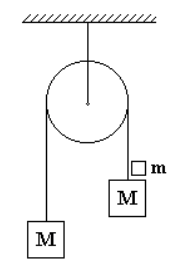
\includegraphics[width=0.2\linewidth]{imagensdinamicanewton/poliamovelexemplo03.png}};
  \end{scope}
\end{tikzpicture}
\captionof{figure}{}
\label{fig_mec_poliamovelexemplo3}
} 

\begin{enumerate}
    \item [a)] $\displaystyle \frac{2mMg}{2M + m}$
    \item [b)] $mg$
    \item [c)] $(m - M)g$
    \item [d)] $\displaystyle \frac{mg}{2M + m}$
    \item [e)] outra expressão
\end{enumerate}

\resolucao

Primeiramente, como mostra a Figura \ref{fig_mec_newtonpoliafixaexemploita}, vamos considerar o sistema dos dois blocos da direita como um único corpo de massa $(M+m).$ 

\vspace{0.3cm}
{
\centering
\begin{tikzpicture}
  \begin{scope}[blend mode=multiply]
    \node {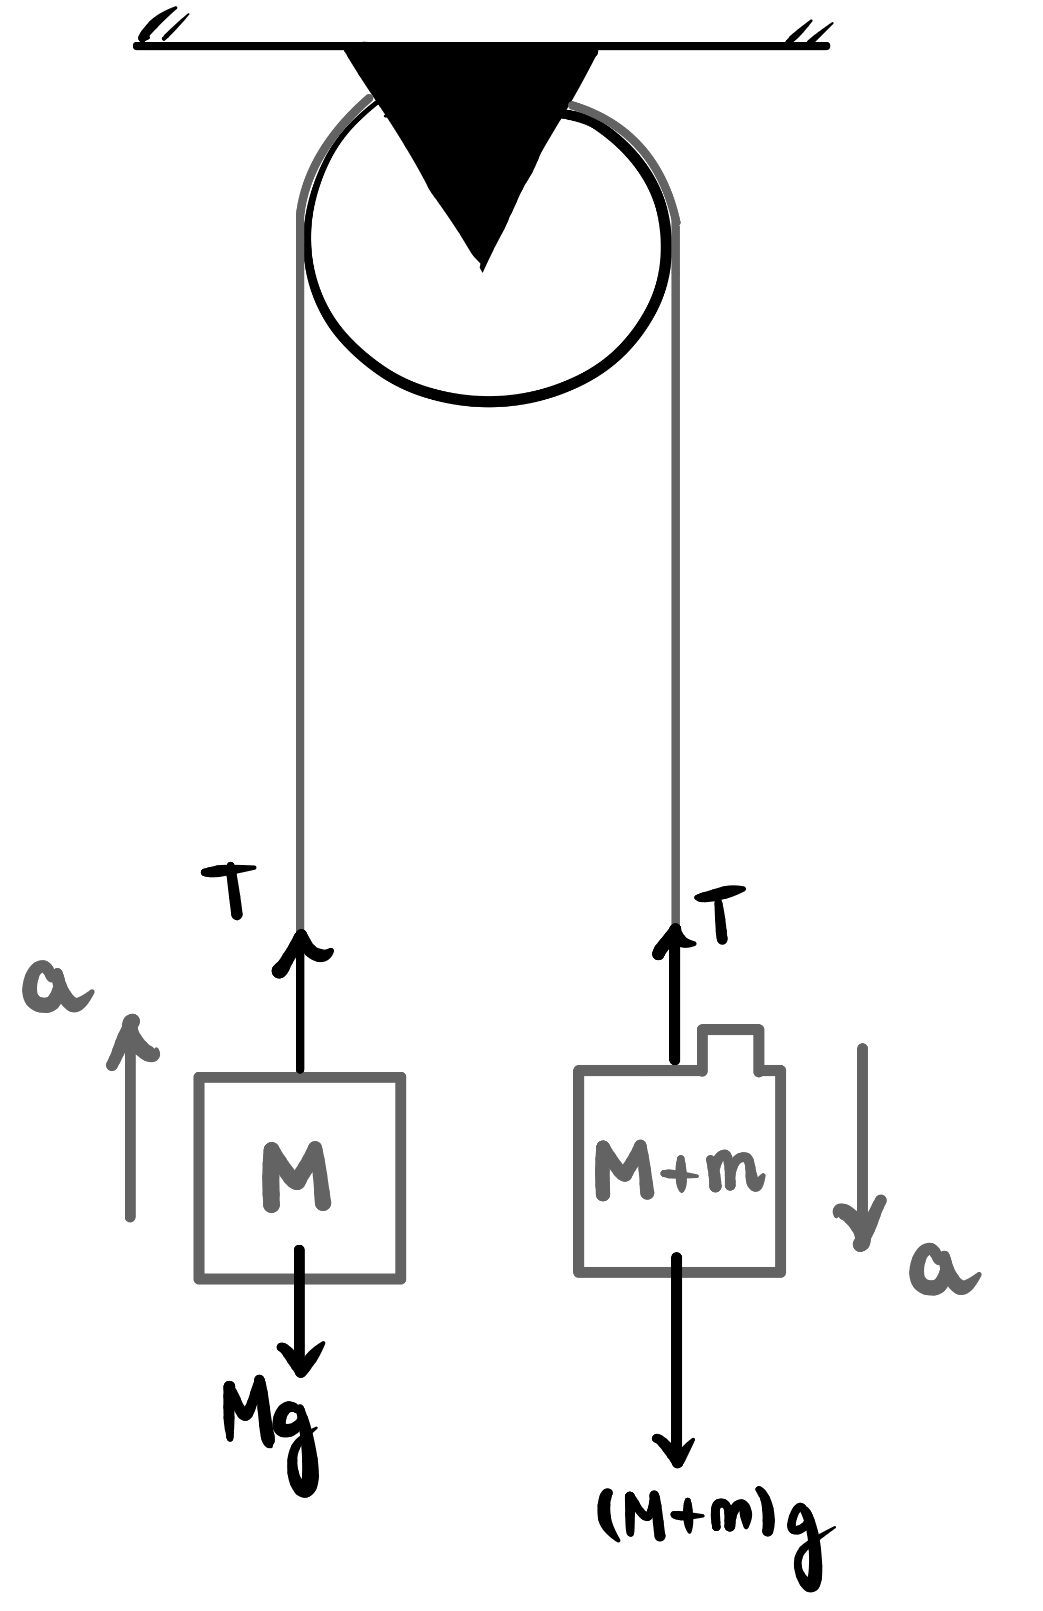
\includegraphics[width=0.22\linewidth]{imagensdinamicanewton/newtonpoliafixaexemploita.png}};
  \end{scope}
\end{tikzpicture}
\captionof{figure}{}
\label{fig_mec_newtonpoliafixaexemploita}
} 
\vspace{0.3cm}


Sendo assim, o cálculo da aceleração $a$ do sistema se dá através da aplicação da Segunda Lei de Newton:

\begin{align}
    \text{Bloco de massa $M$:}& \quad T - Mg = Ma \nonumber \\
    \text{Bloco de massa $(M+m)$:}& \quad (M+m)g - T  = (M+m)a, \nonumber
\end{align}

\noindent que, somando, nos leva a

$$ a = \dfrac{mg}{(2M+m)}.$$

Munidos de tal valor, avaliemos agora as forças que atuam exclusivamente no bloco de massa $m$: o seu peso $P=mg,$ vertical e para baixo; e a normal $N$ trocada com o bloco de massa $M$, que atua verticalmente para cima. Assim, a resultante de tais forças deve gerar no bloquinho a mesma aceleração $a$ que o sistema inteiro possui:

$$F_\text{R} = ma \implies mg - N = m \cdot \dfrac{mg}{(2M+m)} \implies \boxed{N = \dfrac{2Mm}{(2M+m)}g \implies \text{letra A}.}$$

\end{exemplo}







\begin{secnivel}[Força na Polia Móvel]{I}{Força na Polia Móvel}
  
  \eqLdois{dem}{eq_newton_poliamovel}{F_\text{FINAL}=F \cdot2^n}

\end{secnivel}






\secgfe{De onde vem}


A Equação \eqref{eq_newton_poliamovel} mostra como varia uma força $F$, aplicada na extremidade de um sistema de polias à medida que passa por cada polia móvel. Em tal equação, $n$ é o número de polias móveis, $F$ é a força feita por um agente em uma extremidade, como indica a Figura \ref{fig_mec_poliamoveldemonstracao}, e $F_\text{FINAL}$ é a força final que chegará no bloco na última extremidade. 

Em bom português, a Equação \eqref{eq_newton_poliamovel} diz que a força feita pelo menino dobra de valor a cada nova polia móvel no sistema.

\vspace{0.3cm}
{
\centering
\begin{tikzpicture}
  \begin{scope}[blend mode=multiply]
    \node {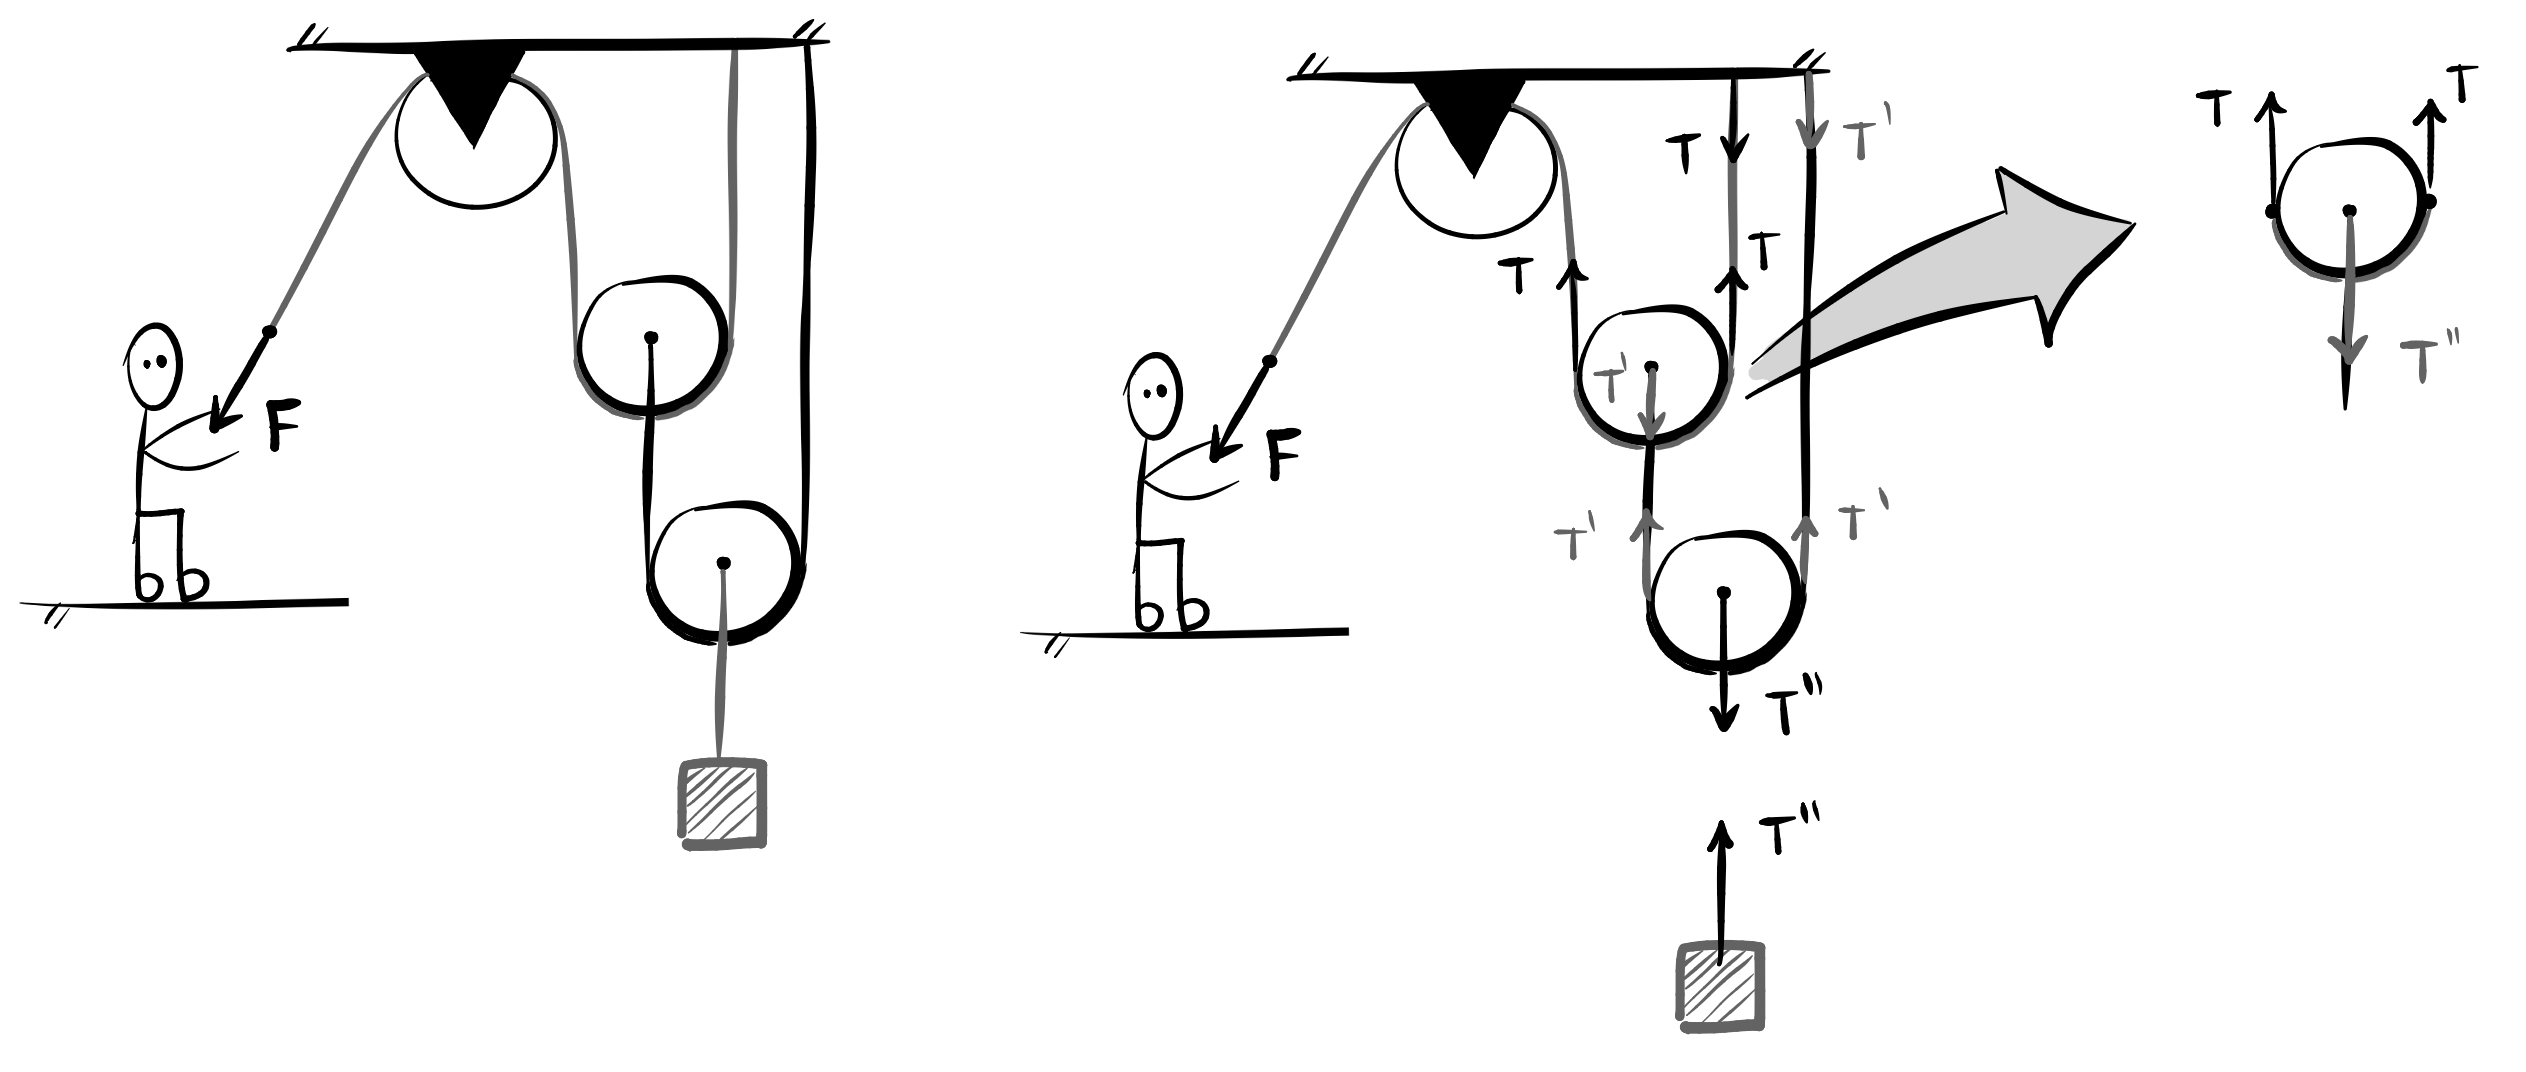
\includegraphics[width=0.8\linewidth]{imagensdinamicanewton/poliamovelprovamatematica.png}};
  \end{scope}
\end{tikzpicture}
\captionof{figure}{Entendendo o sistema de polias móveis.}
\label{fig_mec_poliamoveldemonstracao}
} 
\vspace{0.3cm}

Para entender porque isso funciona assim, é preciso recapitularmos duas ideias centrais:

\begin{enumerate}
    \item [(i)] A força de tração ao longo de um fio ideal é sempre a mesma. Isso vale sempre ao longo de um mesmo fio, e foi demonstrado no desenvolvimento da Equação \eqref{eq_newton_terceiraleinewton}.

    \item [(ii)] Uma polia ideal (que é o que sempre teremos) é aquela em que sua massa é tão pequena que a consideramos nula, isto é, $m_p \approx 0.$ Isso já foi levantado no desenvolvimento da Equação \eqref{eq_newton_poliafixa}.
\end{enumerate}

Note, no sistema da Figura \ref{fig_mec_poliamoveldemonstracao}, que temos uma polia fixa, presa ao teto, e na sequência duas polias móveis. As polias móveis são aquelas que, como o próprio nome diz, não estão fixadas de forma rígida em nenhuma parede e, portanto, podem se mover. Perceba que os fios que passam por tais polias estão presos no teto, mas as polias em si não o estão, de modo que possuem liberdade para se mover.

Note, também, que existem diversos fios no sistema: o primeiro é aquele que o menino puxa. Ele vai das mãos do menino, passa pela polia fixa, depois passa pela polia móvel e se prende no teto. Ao longo de todo esse fio, por ser ideal, a tração será sempre a mesma: $T=F$, como mostra a segunda imagem da figura.

O segundo fio é aquele que conecta o centro da primeira polia móvel, passa pela segunda polia móvel e se prende no teto. Como mudamos o fio, a tração já não tem nenhuma obrigatoriedade de ser manter a mesma. Chamemo-la de $T',$ o que está representando na segunda imagem da figura: ao longo de todo este fio a tração é sempre $T'.$

O terceiro fio seria aquele fio retilíneo que conecta a segunda polia móvel ao bloco. Novamente, como trata-se um novo fio, a tração pode assumir um outro valor -- que será sempre a mesma ao longo de tal fio. Chamemos tal valor de $T'',$ o que está representando na segunda imagem da figura.

Agora que compreendemos os diferentes fios e nomeamos as forças em cada um deles, vamos analisar a Segunda Lei de Newton para a primeira polia móvel, como destacado no último desenho à direita da Figura \ref{fig_mec_poliamoveldemonstracao}. Se a força $F$ aplicada pelo menino for suficiente para erguer o bloco, tal polia irá acelerar verticalmente para cima, uma vez que o sistema como um todo é puxado para cima. Digamos que a aceleração da polia de massa $m_p$ é $a_p.$ Assim, pela Segunda Lei de Newton, teremos, para a primeira polia móvel:

$$ F_{\text{R}} = m a \implies 2T - T'= \cancelto{0}{m_p} \cdot a_p \implies  2T - T' = 0 \implies \boxed{T'= 2T.}$$

Ou seja, ainda que a polia esteja acelerando junto ao bloco, por ter massa nula, a Segunda Lei de Newton nos diz que, em uma polia ideal, a força resultante sempre será zero. Para tal, é necessário que a tração no novo fio logo abaixo da polia móvel seja o dobro da tração no fio superior, a fim de fazer com que a resultante das forças na polia móvel seja nula. A mesma análise para a segunda polia móvel nos levaria a concluir que $T''= 2T',$ ou seja, a força dobraria novamente ao se passar por uma polia móvel.

Dizemos, portanto, que um sistema com polias móveis oferece vantagem mecânica: a força se multiplica por 2 a cada nova polia móvel no sistema, fazendo com que, por meio da aplicação de uma pequena força $F$ em um extremo, seja possível erguer corpos extremamente massivos no outro extremo, bastando para isso adicionar um número suficiente de polias móveis capaz de fazer a força dobrar até conseguir superar o peso de tal corpo.

Desse modo, ao fazer uma força $F$ em um fio na extremidade de um sistema com várias polias móveis, a força irá multiplicar por 2 a cada polia móvel pela qual passar, de modo que a força final que teremos no extremo será

$$ F_\text{FINAL}=F\cdot  \underbrace{2 \cdot 2 \cdot 2 \dots \cdot 2}_{\text{n vezes}} = F \cdot 2^n, $$

\noindent que é exatamente o que diz a Equação \eqref{eq_newton_poliamovel}.


\secgfe{Onde é usada}

Os contextos mais comuns de aplicação aqui são os mesmos daqueles da polia fixa: aparelhos de academia ou dispositivos em que se deseja carregar grandes massas. Aqui, como temos um dispositivo que oferece vantagem mecânica, ele é particularmente interessante para carregar objetos extremamente pesados, o que poderá ser feito por meio da aplicação de pequenas forças, como a Equação \eqref{eq_newton_poliamovel} indica.

Considere, por exemplo, a situação da Figura \ref{fig_mec_poliamovelteoria}. Qual seria a força necessária a ser feita para carregar o bloco de massa $m=10kg$ com velocidade constante?

\vspace{0.3cm}
{
\centering
\begin{tikzpicture}
  \begin{scope}[blend mode=multiply]
    \node {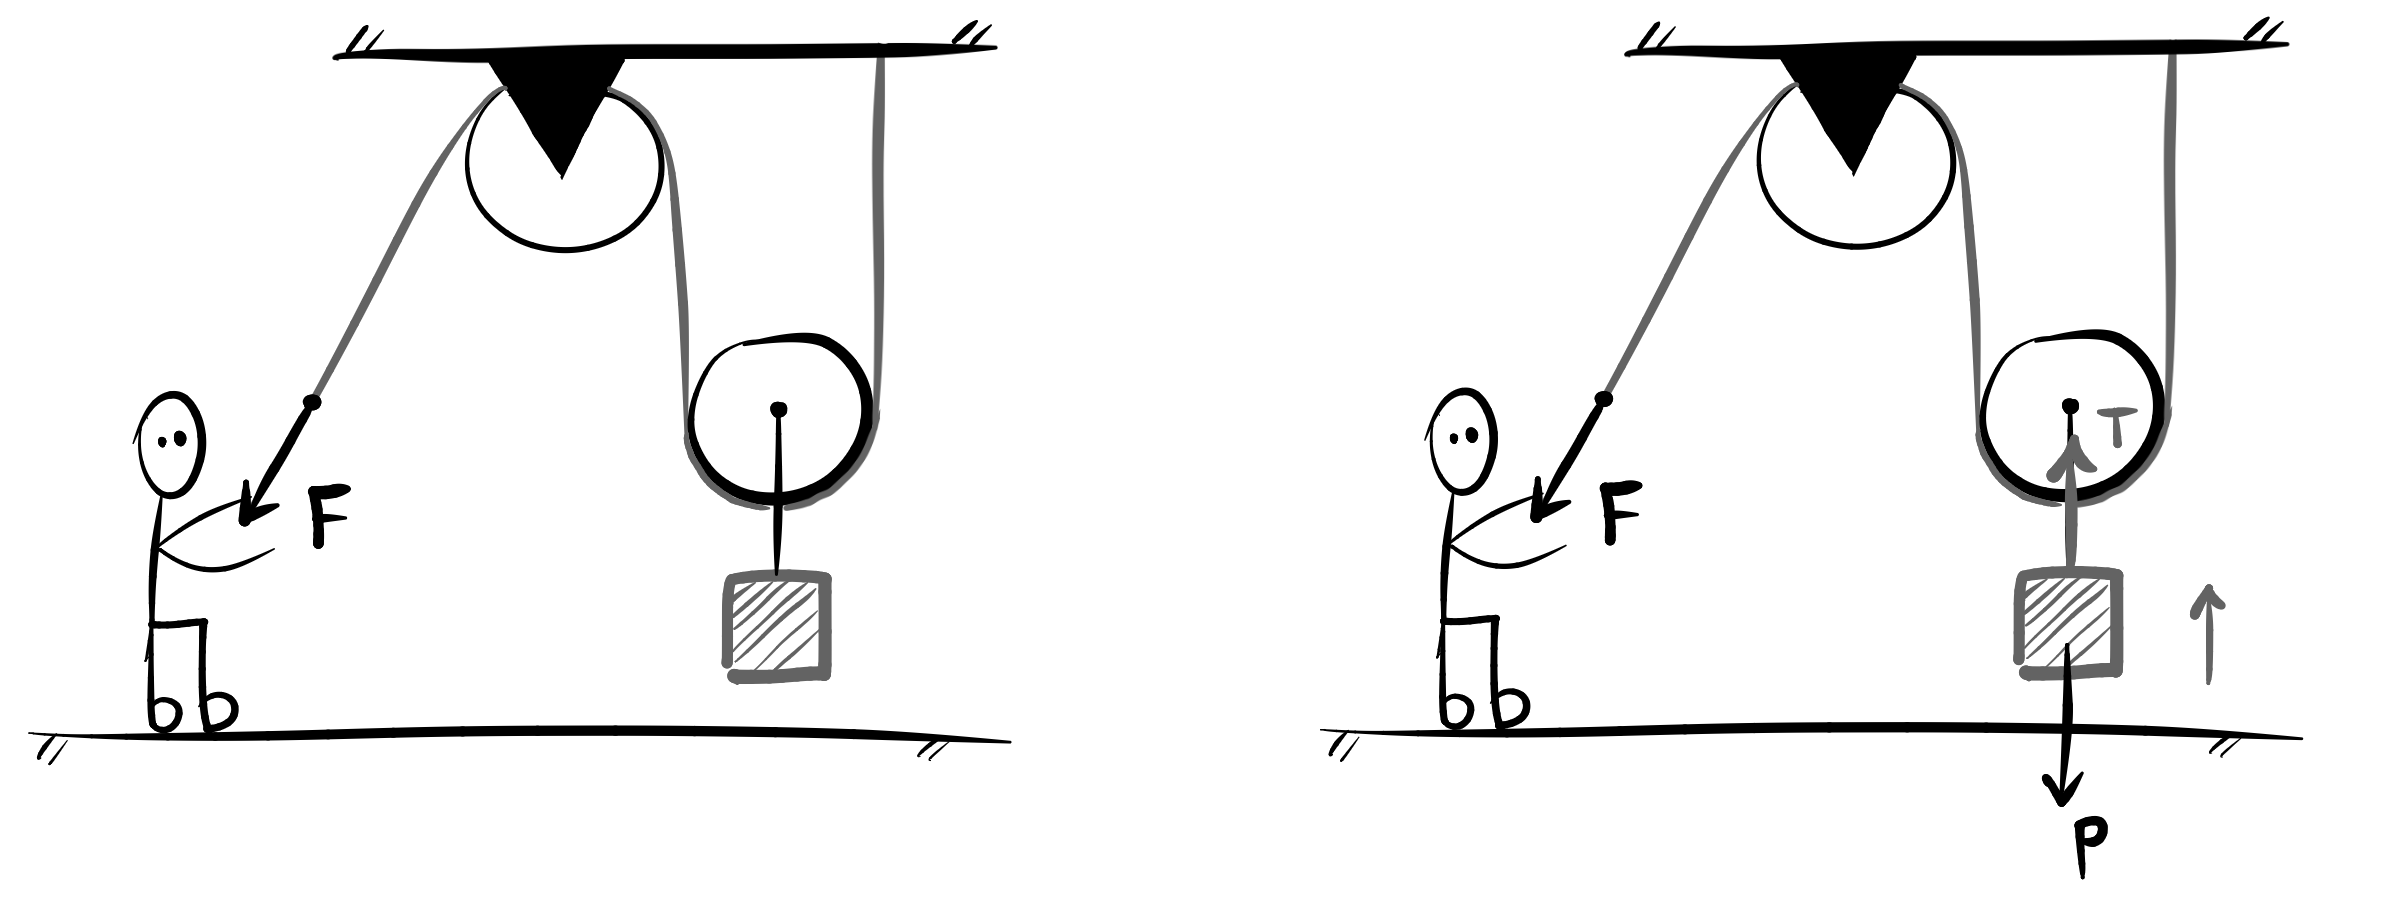
\includegraphics[width=0.6\linewidth]{imagensdinamicanewton/poliamovelteoria.png}};
  \end{scope}
\end{tikzpicture}
\captionof{figure}{Erguendo bloco com um sistema de polias.}
\label{fig_mec_poliamovelteoria}
} 
\vspace{0.3cm}

Para subir com velocidade constante o bloco estará em equilíbrio, isto é, $F_\text{R}=0.$ Como mostra a segunda imagem da Figura \ref{fig_mec_poliamovelteoria}, isso quer dizer que $T=P=100$N. Como a força feita pelo menino na extremidade da direita irá dobrar a cada polia móvel -- e temos apenas uma polia móvel -- ele pode fazer uma força de apenas $50$N, que se manterá constante ao longo da polia fixa e dobrará de valor após passar pela polia móvel, originando a força de $100$ N para erguer a caixa com velocidade constante.

Parece mágica em um primeiro momento: é possível erguer um bloco de 10kg fazendo a força que seria necessária para erguer um bloco de 5kg. Mas não tem nada de errado nisso: não existe, na Física, nenhuma \textit{lei de conservação da força}, de modo que um sistema que multiplique o valor da força e ofereça vantagem mecânica, como o sistema de uma polia móvel, é perfeitamente viável e fisicamente possível, por mais que cause um certo estranhamento em um primeiro momento. Veremos, ao estudar a Lei de Conservação da Energia, que tal sistema não só é possível como também deve ser exatamente desse modo, a fim de respeitar tal lei da Física.


\secgfe{Erros comuns}

Em geral os problemas irão envolver polias fixas e móveis na mesma situação. O erro mais comum é o estudante não conseguir identificar quais são as polias fixas e quais são as móveis, e acabar usando que a força dobra ao passar por uma polia fixa, por exemplo.

Note, na Figura \ref{fig_mec_roldanafixaemovel}, que todas as quatro polias da parte de cima estão fixas no teto, logo, tratam-se de polias fixas, sem vantagem mecânica. Já as quatro polias da parte inferior são móveis -- elas não estão fixas\footnote{Algum leitor poderia pensar \textit{``ora, mas elas estão fixadas na barra abaixo, que está presa ao bloco.''} Sim, mas perceba que o bloco não está fixado em lugar algum, logo, todo esses sistema -- polias, barra e bloco -- pode se mover. Portanto, tratam-se de polias móveis. Se um objeto está fixado em um corpo que pode se mover, logo, tal objeto também poderá se mover, sendo, portanto, um corpo móvel e não fixo.} e podem se mover junto com o bloco.

\vspace{0.3cm}

{
\centering
\begin{tikzpicture}
  \begin{scope}[blend mode=multiply]
    \node {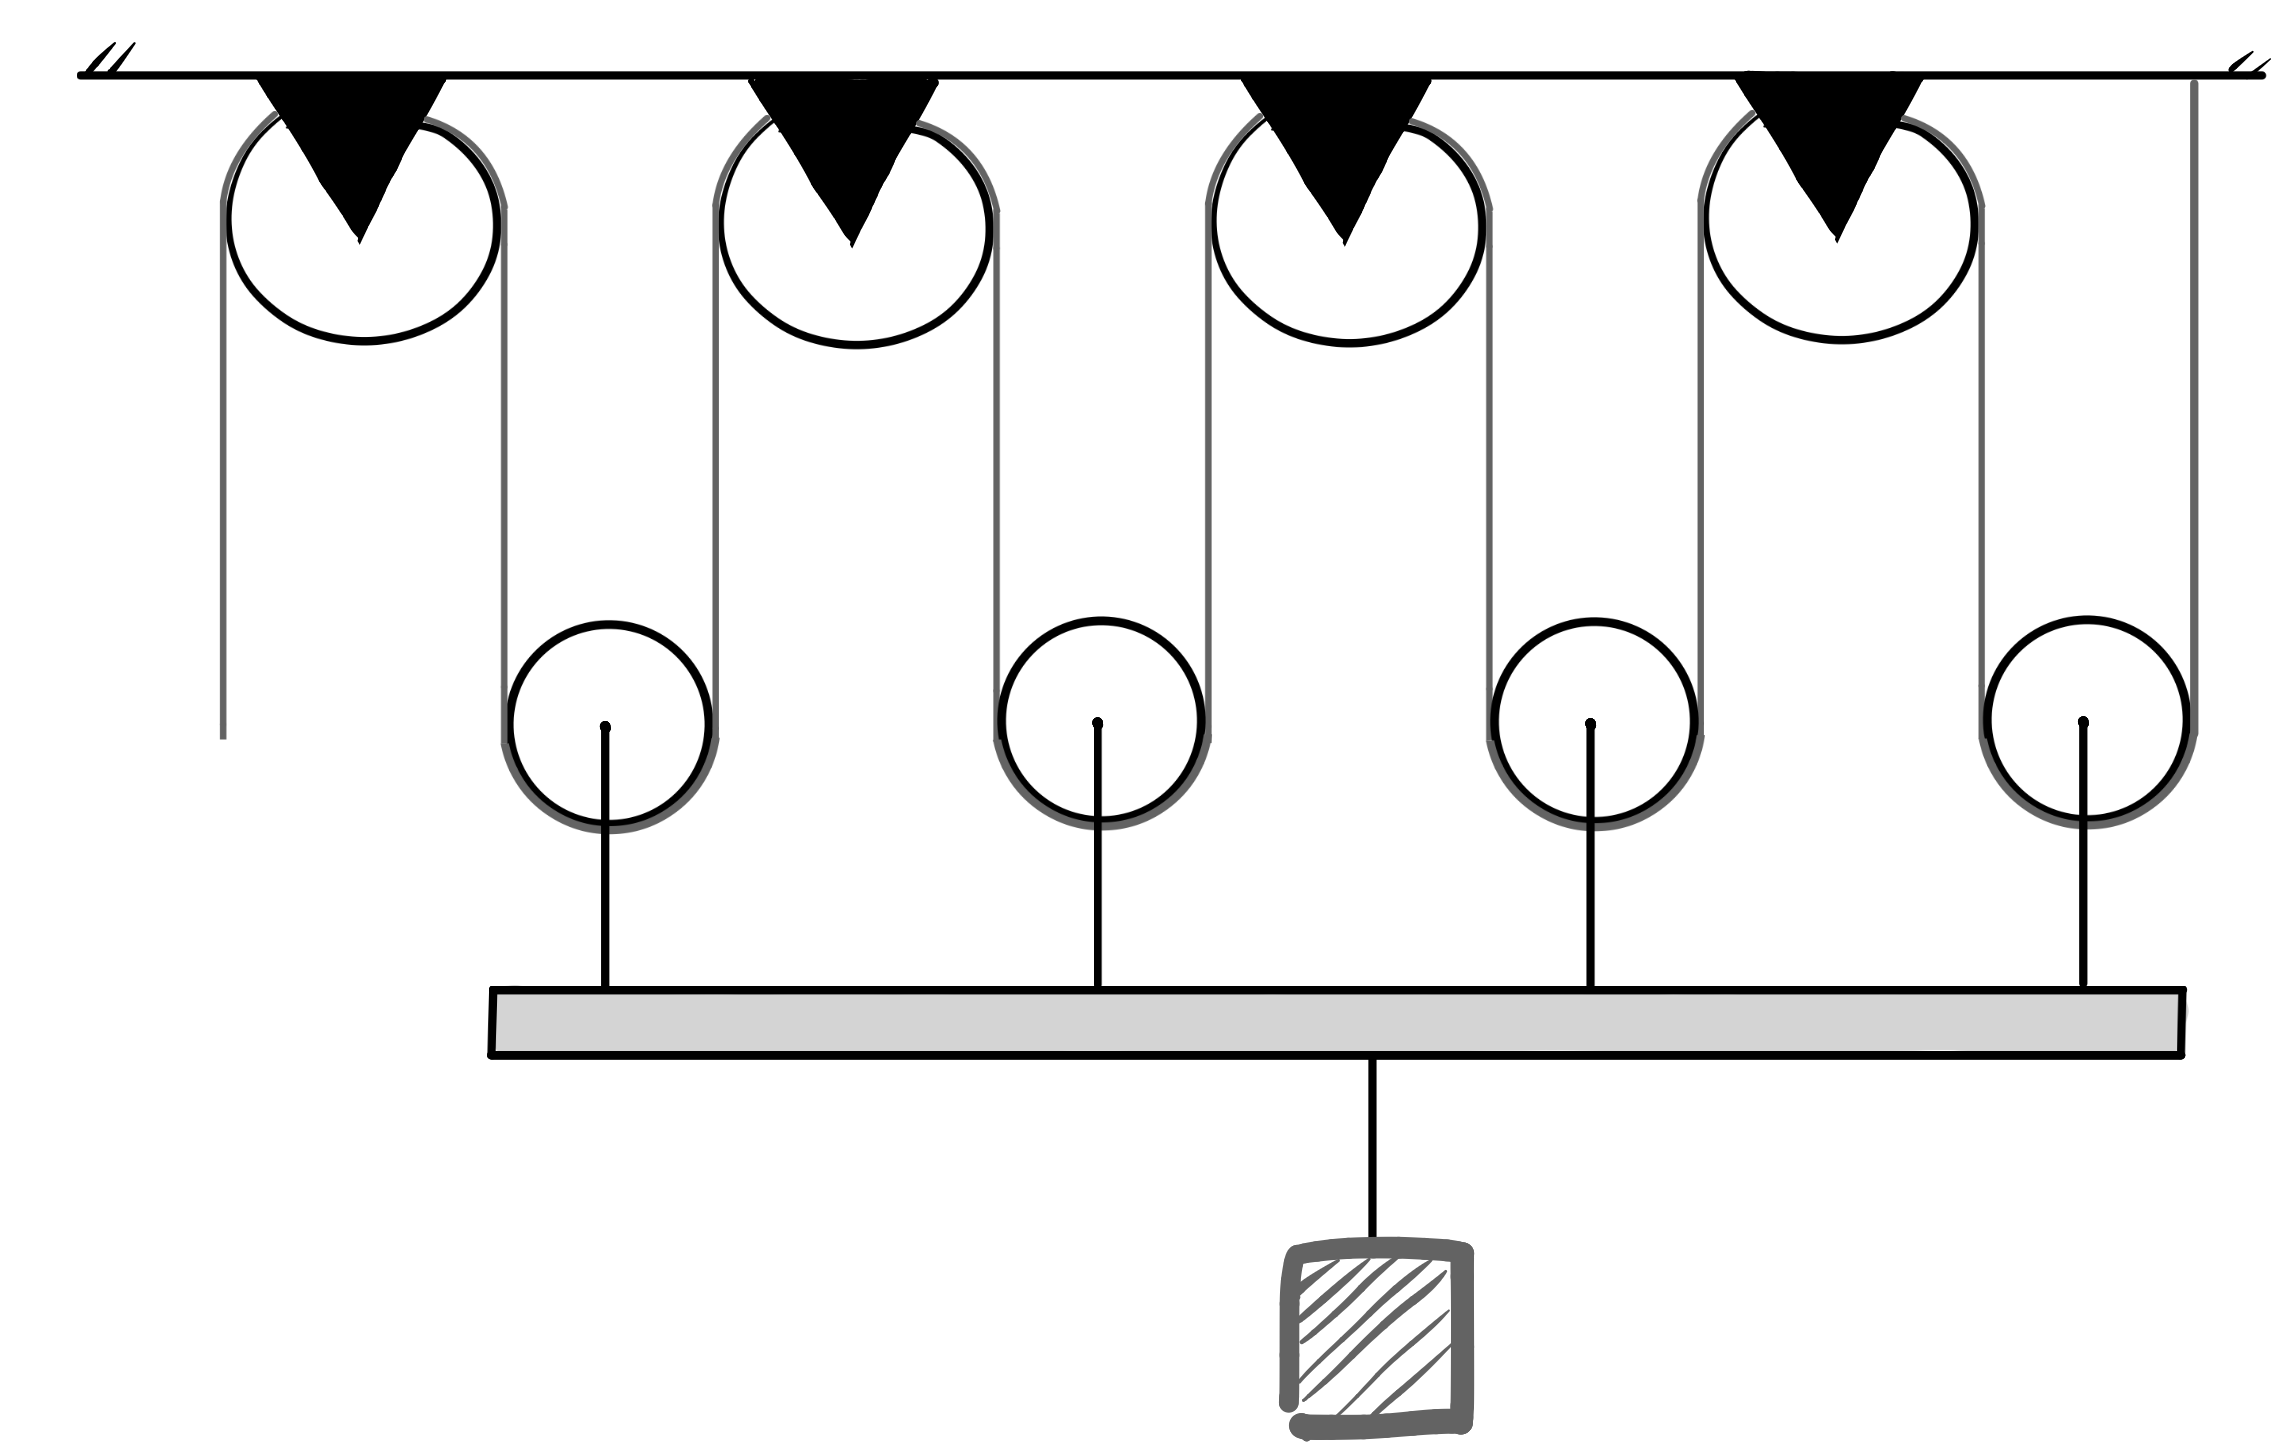
\includegraphics[width=0.45\linewidth]{imagensdinamicanewton/roldanafixaemovel.png}};
  \end{scope}
\end{tikzpicture}
\captionof{figure}{Roldanas fixas e móveis.}
\label{fig_mec_roldanafixaemovel}
} 
\vspace{0.3cm}



\secgfe{Observações}

Vamos discorrer brevemente sobre a razão pela qual o sistema multiplicador de forças é fisicamente possível. Isso será entendido com mais profundidade ao estudarmos o princípio da Conservação da Energia Mecânica, no estudo da Equação \eqref{eq_energia_conservacaodaenergiamecanica}.


Observe a situação da Figura \ref{fig_mec_poliamovelconservacao}. Tal situação mostra que, ao puxar o fio e fazer com que a polia móvel (e, consequentemente, o bloco, uma vez que este está preso em tal polia por um fio) se mova para cima de um certo tanto $x$, foi necessário que o menino puxasse o fio do dobro desse valor, isto é, de $2x$. Isso ocorre porque o fio sai da polia fixa, desce pela esquerda da polia móvel e sobe pela sua direita, prendendo-se ao teto. Sendo assim, ao puxar o fio de 2 metros, por exemplo, será como se tivéssemos puxado 1 metro da parte esquerda e 1 metro da parte direita. Ou seja, o sistema só sobe 1 metro, ainda que se puxe 2 metros de fio.




\vspace{0.3cm}
{
\centering
\begin{tikzpicture}
  \begin{scope}[blend mode=multiply]
    \node {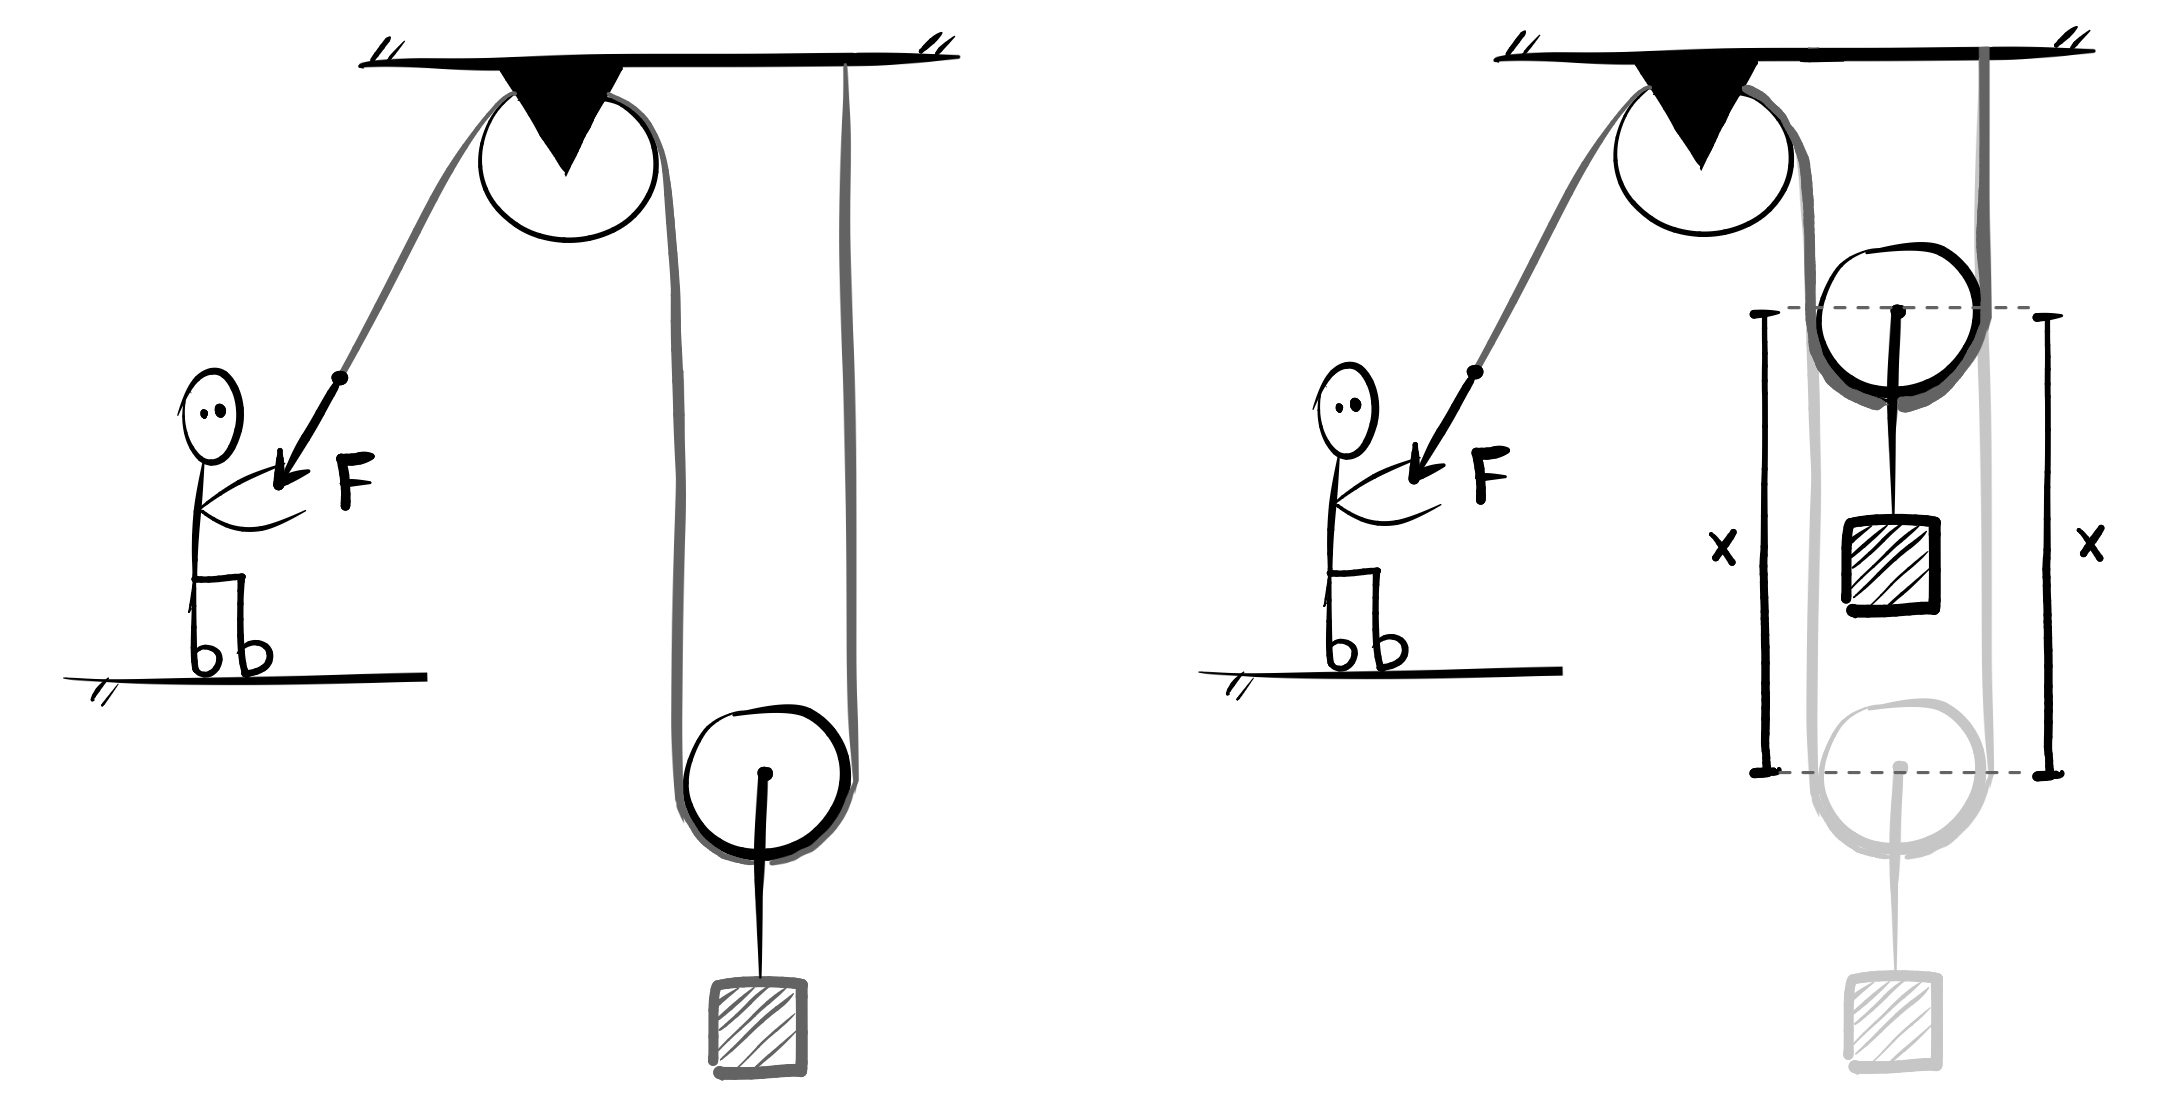
\includegraphics[width=0.6\linewidth]{imagensdinamicanewton/poliamoveleconservacaoenergia.png}};
  \end{scope}
\end{tikzpicture}
\captionof{figure}{O preço a se pagar neste sistema: para erguer o bloco de um tanto $x$ é preciso puxar o dobro de corda, isto é, $2x$.}
\label{fig_mec_poliamovelconservacao}
} 
\vspace{0.3cm}

No final do dia esse é o preço que se paga em um sistema como esse, nada é de graça: a força feita pelo menino é metade da força que chega ao bloco, porém a quantidade de fio que o menino deve puxar será sempre o dobro do tanto que o bloco se move. Assim, o menino precisará puxar a corda sempre com o dobro da velocidade com que o bloco se moverá: para subir o bloco a uma velocidade de 3 m/s é preciso que o menino puxe 6 metros de corda a cada segundo. 

Como veremos no estudo da Equação \eqref{eq_energia_conservacaodaenergiamecanica}, o produto da força feita pelo tanto de fio que se puxa (seu deslocamento) é justamente igual à energia dispendida pelo menino. Logo, ele faz metade da força, mas puxa o dobro de corda, de modo que a energia que ele gasta é exatamente a mesma que chega ao bloco e o suspende.

Assim, apesar de se fazer menos força, o esforço (energia dispendida) é o mesmo. Troca-se fazer menos força por puxar mais corda -- o que, em muitos casos, é uma excelente troca.


\vspace{0.3cm}


\begin{exemplo}[Nível I (EsPCEx 2020)]\label{exemplo_newton_poliamovel0}

O sistema de polias, sendo uma fixa e três móveis, encontra-se em equilíbrio estático, conforme mostra o desenho. 
A constante elástica da mola, ideal, de peso desprezível, é igual a $50\,\text{N/cm}$ e a força $F$ na extremidade da corda é de intensidade igual a $100\,\text{N}$. 
Os fios e as polias, iguais, são ideais.

\vspace{0.3cm}
{
\centering
\begin{tikzpicture}
  \begin{scope}[blend mode=multiply]
    \node {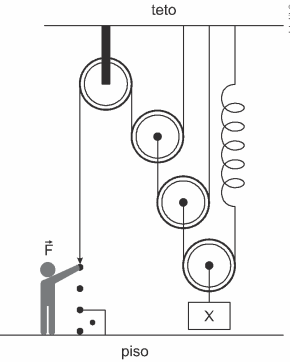
\includegraphics[width=0.27\linewidth]{imagensdinamicanewton/poliamovelexemplo2.png}};
  \end{scope}
\end{tikzpicture}
\captionof{figure}{}
\label{fig_mec_poliamovelexemplo2}
} 
\vspace{0.3cm}

O valor do peso do corpo $X$ e a deformação sofrida pela mola são, respectivamente,
\begin{enumerate}
    \item [a)]$800\,\text{N}$ e $16\,\text{cm}$
    \item [b)]$400\,\text{N}$ e $8\,\text{cm}$
    \item [c)]$600\,\text{N}$ e $7\,\text{cm}$
    \item [d)]$800\,\text{N}$ e $8\,\text{cm}$
    \item [e)]$950\,\text{N}$ e $10\,\text{cm}$
\end{enumerate}

\resolucao

A força $F$ feito pelo menino irá dobrar a cada polia móvel pela qual passar, de modo que, para 3 polias móveis, a força final será

$$ F_\text{FINAL} = F \cdot 2^3 = 8F = 8 \cdot 100 = 800 \text{N.}$$

Assim, se o bloco está em equilíbrio, é porque tal força é exatamente igual ao seu peso: $P=800 \text{N}.$

O fio que possui tração de 800 N é aquele que conecta o bloco à última polia. Logo, o fio em que a mola está conectada é outro: ao longo deste fio a tração é de 400N. Observe em detalhes o diagrama das forças na Figura \ref{fig_mec_poliamoveldemonstracao} em caso de dúvida.

Assim, para a mola, teremos:

$$F = kx \implies 400 = 50x \implies x = 8 \text{ cm},$$

\noindent de modo que a letra D é a resposta correta.


\end{exemplo}



\vspace{0.3cm}


\begin{exemplo}[Nível II]\label{exemplo_newton_poliamovel02}

Considere o sistema da Figura \ref{fig_mec_poliamovelexemploresolvido21}. Qual deve ser o valor da massa $M$ para que ela fique em equilíbrio?

\vspace{0.3cm}
{
\centering
\begin{tikzpicture}
  \begin{scope}[blend mode=multiply]
    \node {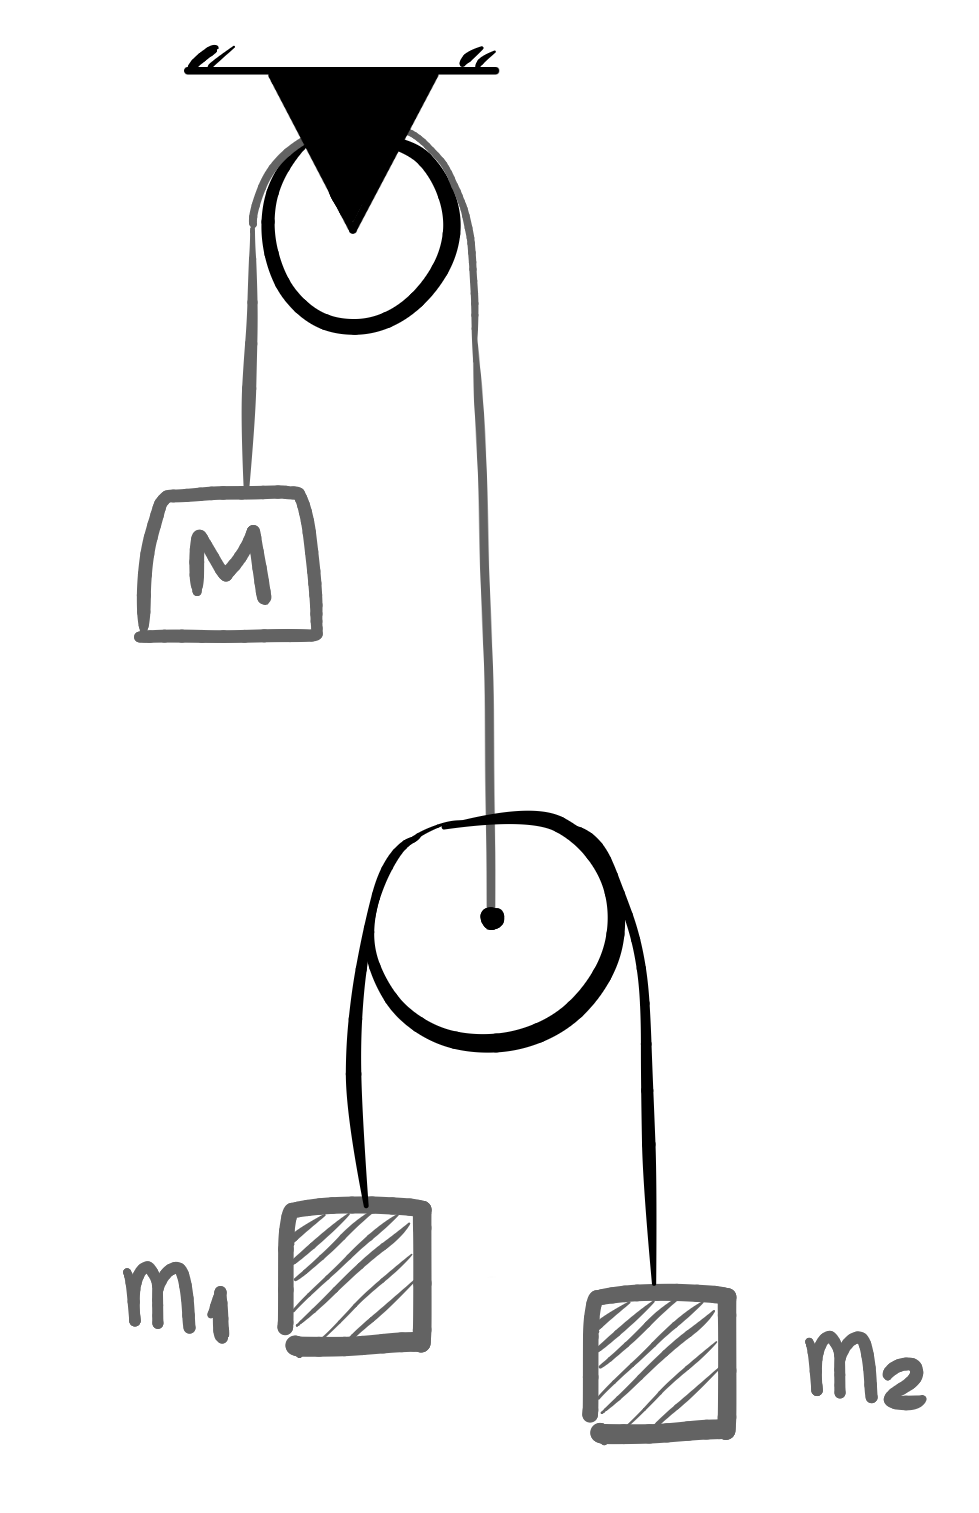
\includegraphics[width=0.22\linewidth]{imagensdinamicanewton/poliamovelexemploresolvido21.png}};
  \end{scope}
\end{tikzpicture}
\captionof{figure}{}
\label{fig_mec_poliamovelexemploresolvido21}
} 
\vspace{0.3cm}


\resolucao

O leitor mais ingênuo poderia pensar que a massa $M$ deveria equivaler à soma das massas do lado direito, isto é, $M = m_1+m_2.$ Isso até seria verdade se o sistema inteiro estivesse em equilíbrio, o que não ocorre.

\medskip

As massas da direita, $m_1$ e $m_2,$ certamente não estarão em equilíbrio se $m_1 \neq m_2$ elas certamente estarão acelerando. Queremos, contudo, que a polia móvel na qual elas estão conectadas permaneça em equilíbrio. Como acelerações são geradas por forças, o fato do sistema da direita estar acelerado irá alterar as trações nos fios, o que irá afetar a dinâmica do sistema e, portanto, irá alterar o valor de massa $M$ necessário para manter  a polia móvel em equilíbrio. 

\vspace{0.3cm}
{
\centering
\begin{tikzpicture}
  \begin{scope}[blend mode=multiply]
    \node {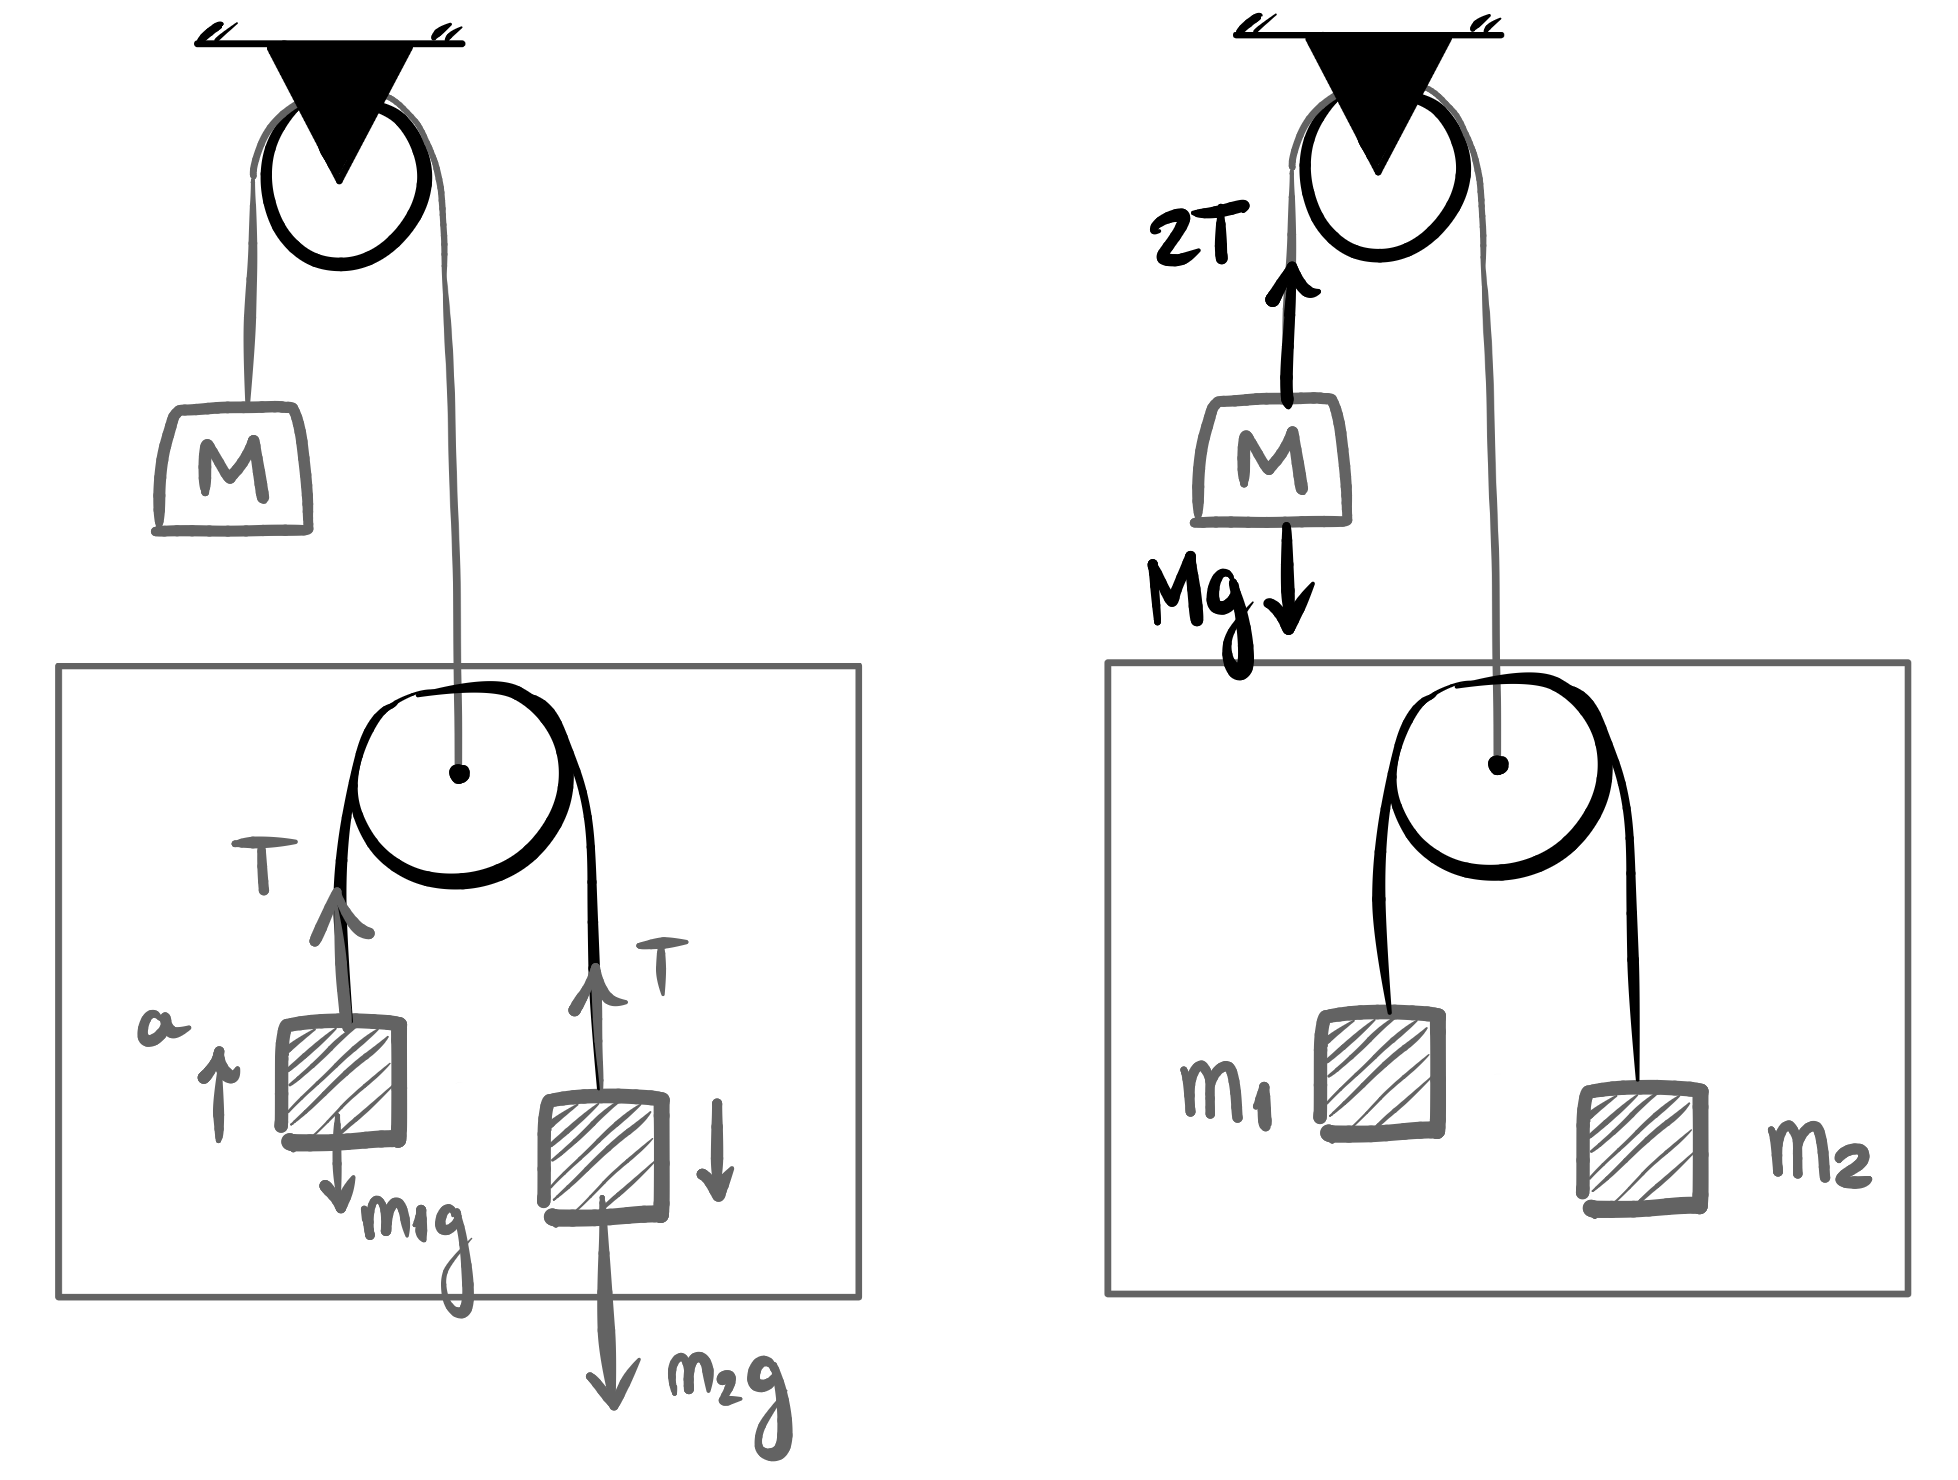
\includegraphics[width=0.6\linewidth]{imagensdinamicanewton/poliamovelexemploresolvido22.png}};
  \end{scope}
\end{tikzpicture}
\captionof{figure}{}
\label{fig_mec_poliamovelexemploresolvido22}
} 
\vspace{0.3cm}

Equacionando a Segunda Lei de Newton para as massas $m_1$ e $m_2,$ supondo $m_2>m_1$, teremos:

\begin{align}
    T - m_1g &= m_1 a \nonumber \\
    m_2g - T &= m_2 a ,\nonumber
\end{align}

\noindent que, somando, nos leva a

$$ a =  \left(\dfrac{m_2 - m_1}{m_2+m_1} \right)g \quad \text{ e } \quad T = \dfrac{2m_1m_2g}{m_1+m_2}.$$

A segunda imagem da Figura \ref{fig_mec_poliamovelexemploresolvido22} mostra que a força no fio que passa pelo bloco de massa $M$ é $2T,$ de modo que, para que ele fique em equilíbrio, é preciso que:

$$ 2T = Mg \implies \boxed{M = \dfrac{4m_1m_2}{m_1+m_2}.}$$

Note que, se $m_1 = m_2,$ teremos $a=0$ e $T = mg, $ como esperado. Neste caso os blocos da direita ficam parados ou em MRU -- de toda forma, se encontram em equilíbrio. Assim, a expressão acima se reduz a $M=2m=m+m,$ que foi nossa intuição inicial.

\medskip

Contudo, se o sistema da direita estiver acelerado, a força necessária a ser feita do lado esquerdo para manter a polia móvel em equilíbrio não será igual à soma dos pesos dos blocos $m_1$ e $m_2$, e sim igual ao peso de um bloco de massa $M=4m_1m_2/(m_1+m_2)$

\medskip 

Façamos uma breve discussão desse resultado. A média aritmética (MA) entre dois números $x_1$ e $x_2$ e sua média harmônica (MH) são definidas como:

$$ MA = \dfrac{x_1+x_2}{2} \quad \text{ e } \quad MH = \dfrac{2}{\dfrac{1}{x_1} + \dfrac{1}{x_2}}.$$

A desigualdade das médias nos diz que $MA \geq MH,$ a igualdade ocorrendo quando os números forem iguais. Logo, teremos:

$$ \dfrac{x_1+x_2}{2} \geq  \dfrac{2}{\dfrac{1}{x_1} + \dfrac{1}{x_2}},$$

\noindent o que se escreve como

$$ x_1+x_2 \geq \dfrac{4x_1x_2}{x_1+x_2}.$$

Fazendo $m_1$ e $m_2$ como sendo os números $x_1$ e $x_2$, teremos

$$ m_1+m_2 \geq \dfrac{4m_1m_2}{m_1+m_2} = M,$$

\noindent ou seja, se o sistema dos blocos $m_1$ e $m_2$ estiver acelerando, como na primeira imagem da Figura \ref{fig_mec_poliamovelexemploresolvido22}, então a massa $M$ que mantém a polia móvel em repouso será sempre menor que a soma das massas $m_1$ e $m_2.$ Ou seja, é mais fácil sustentar o sistema da máquina de Atwood acelerado do que o sistema em equilíbrio.


\end{exemplo}
\vspace{0.3cm}








\begin{exemplo}[Nível III]\label{exemplo_newton_poliamovel03}

O sistema da Figura \ref{fig_mec_poliamovelexemplo222a} é livre de atrito e os fios e polias são ideais. Se a gravidade local vale $g,$ encontre a aceleração de cada bloco.

\vspace{0.3cm}
{
\centering
\begin{tikzpicture}
  \begin{scope}[blend mode=multiply]
    \node {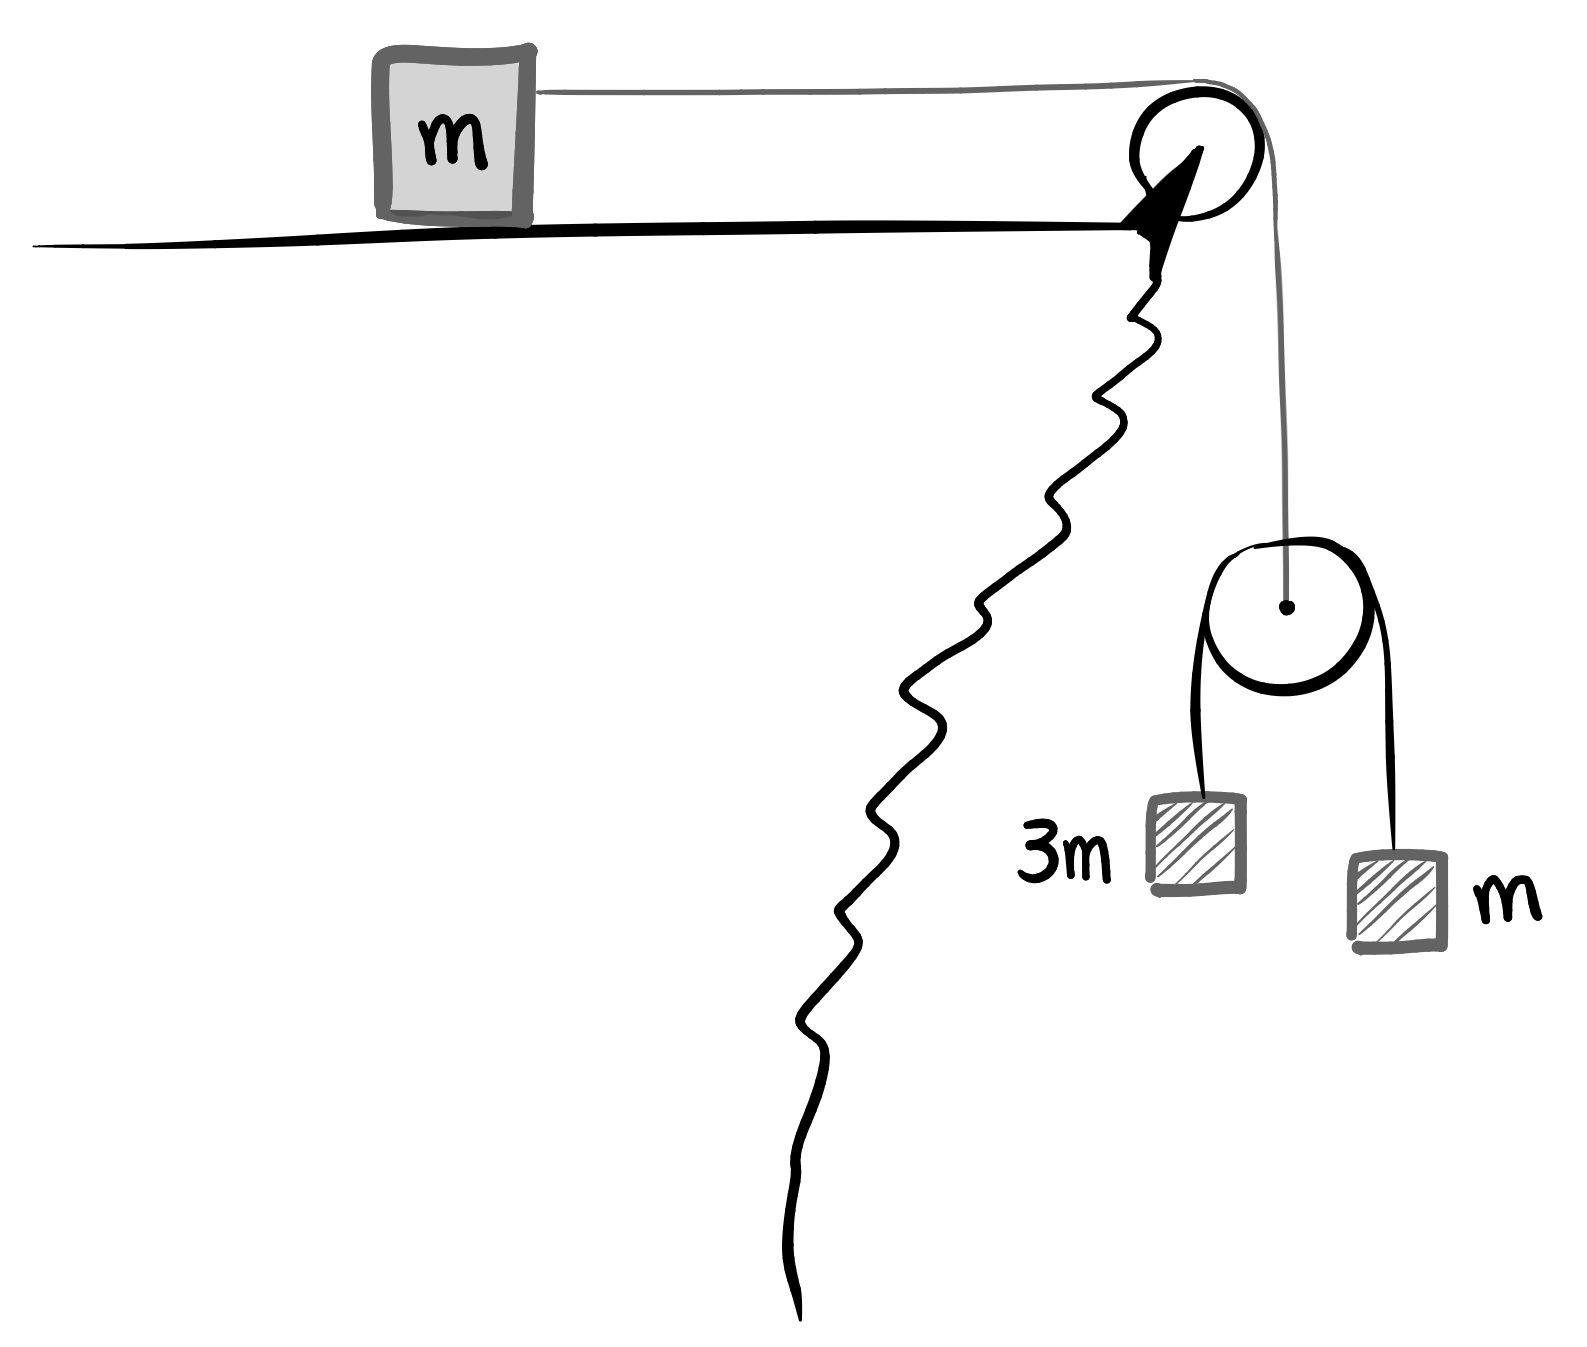
\includegraphics[width=0.4\linewidth]{imagensdinamicanewton/polia movel ex 02.png}};
  \end{scope}
\end{tikzpicture}
\captionof{figure}{}
\label{fig_mec_poliamovelexemplo222a}
} 
\vspace{0.3cm}



\resolucao

Chamemos de bloco $1$ aquele de massa $m$ que está apoiado no solo horizontal. Ele se moverá com aceleração horizontal $a_1=a$ para a direita, como mostra a primeira imagem da Figura \ref{fig_mec_poliamovelexemplo2avancao2}. Com isso, imagine que o sistema dos outros dois blocos estivesse dentro de um elevador: este elevador irá cair verticalmente com a mesma aceleração $a_1$ do bloco horizontal, uma vez que esses dois corpos estão acoplados pelo mesmo fio e devem se mover com a mesma aceleração.


\vspace{0.3cm}
{
\centering
\begin{tikzpicture}
  \begin{scope}[blend mode=multiply]
    \node {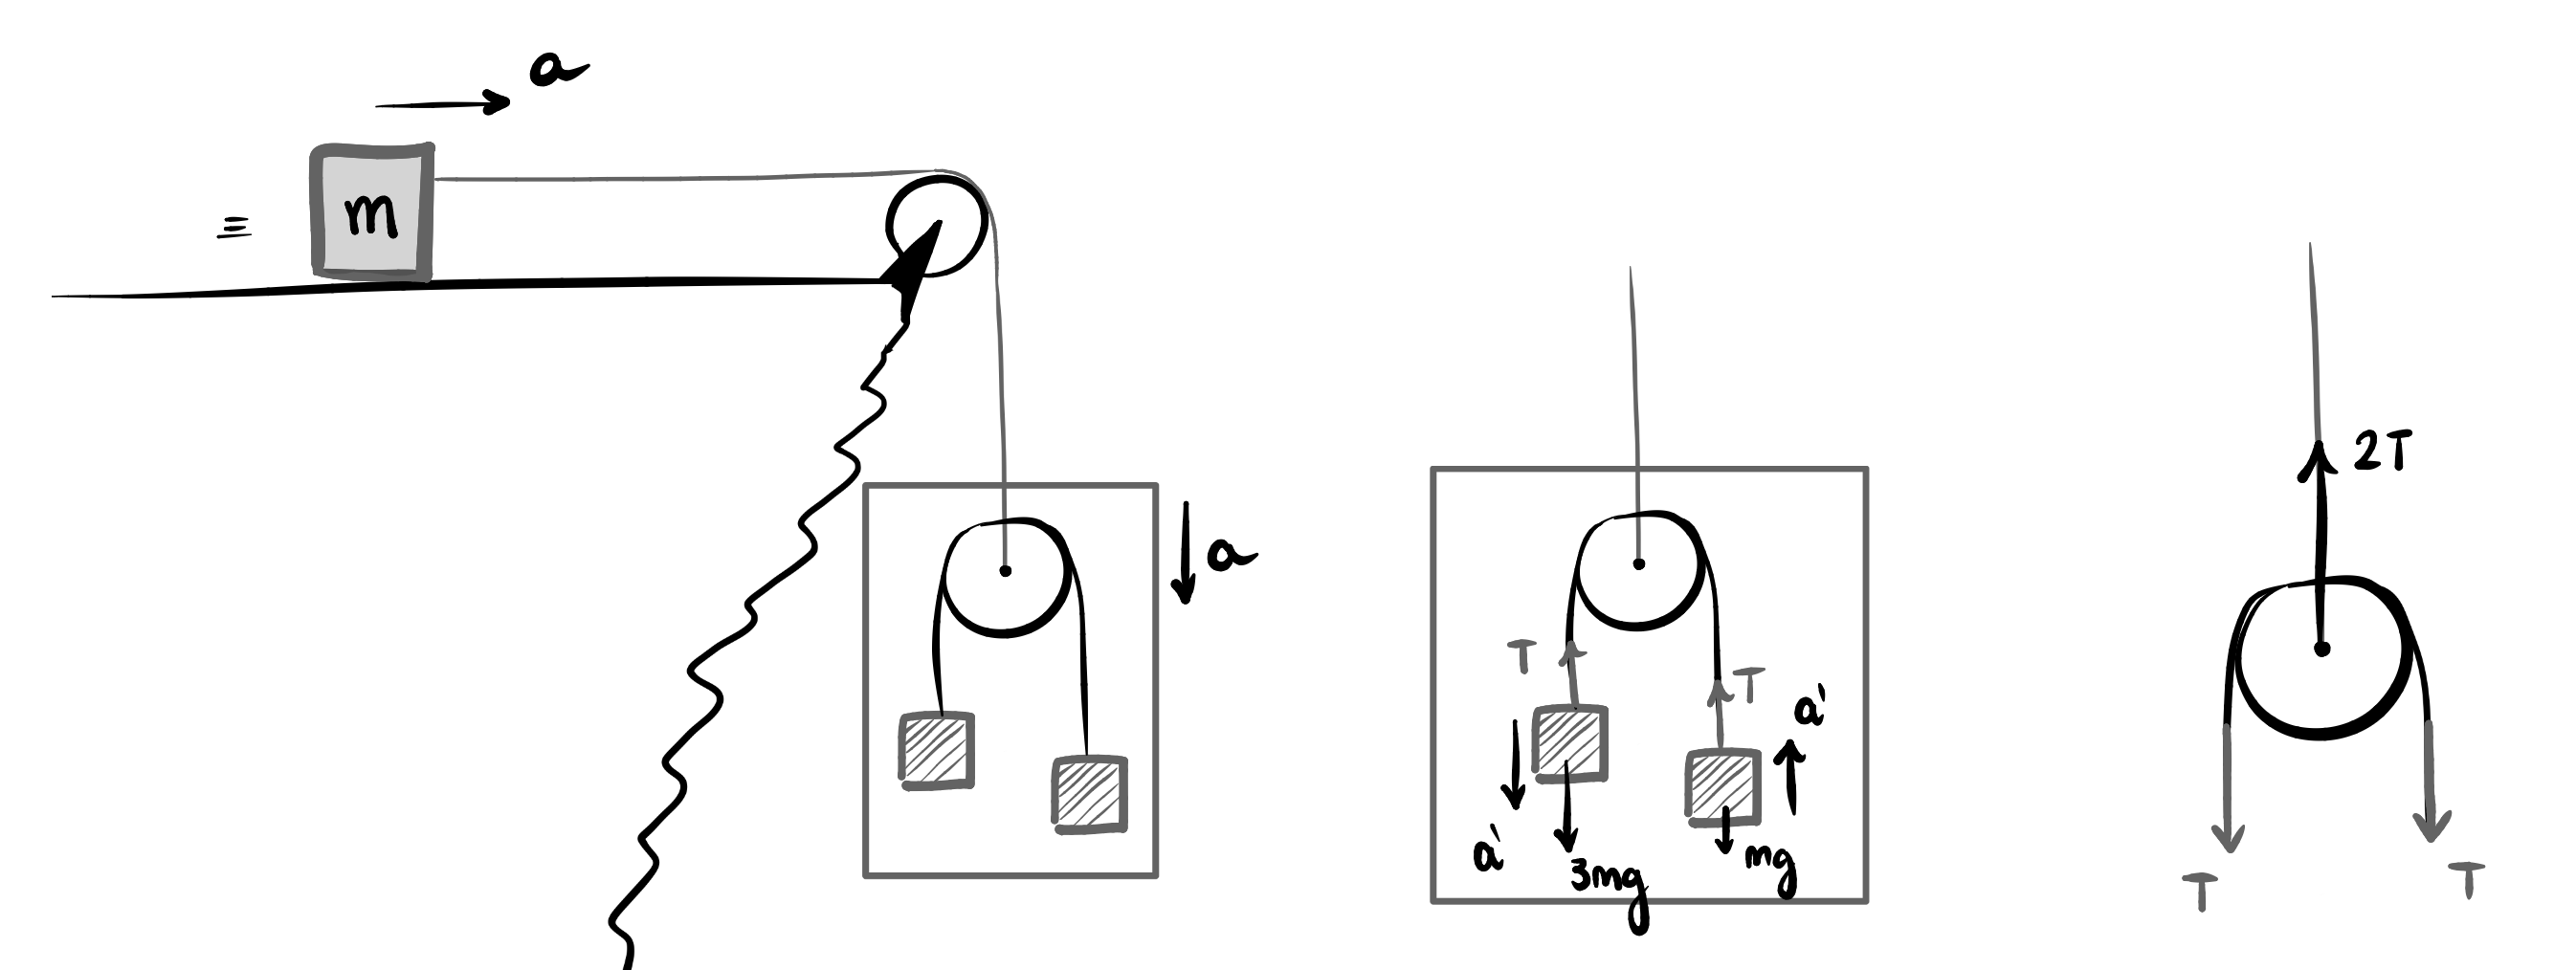
\includegraphics[width=0.9\linewidth]{imagensdinamicanewton/poliamovelexemplo2avancao.png}};
  \end{scope}
\end{tikzpicture}
\captionof{figure}{}
\label{fig_mec_poliamovelexemplo2avancao2}
} 
\vspace{0.3cm}

Contudo, internamente dentro deste elevador, os dois blocos também se movem em movimentos acelerados. Designemos por $a'$ a aceleração destes blocos em relação ao elevador. Logo, as acelerações $a_2$ e $a_3$ dos blocos de massa $3m$ e $m$, internos ao elevador, serão, em relação à Terra, respectivamente iguais a:

\begin{align}
    a_2 &= a_1 + a'  \nonumber \\
    a_3 &= a_1 - a'  \nonumber
\end{align}

Desse modo, a Segunda Lei de Newton para cada um desses blocos diz que

\begin{align}
    3mg - T &= 3 m (a_1 + a') \nonumber \\
    mg-T &=  m (a_1 - a'), \nonumber
\end{align}

\noindent que, subtraindo, nos leva a\footnote{Note que, para o bloco $3$, de massa $m,$ a força resultante foi equacionada para baixo: a força peso menos a tração. Isso foi feito porque partimos da premissa de que sua aceleração total em relação à Terra é para baixo, isto é, ela é $a_3=a_1-a',$ em que $a_1>a'.$}

$$ a_1+2a' = g \quad \text{ e } \quad T = \dfrac{3m(g-a_1)}{2}.$$

A segunda última imagem da Figura \ref{fig_mec_poliamovelexemplo2avancao2} mostra o diagrama de forças na polia móvel: como em toda polia ideal é preciso ter $F_\text{R}=0,$ a tração no fio superior que conecta a polia movel ao bloco horizontal deve ser $2T = 3mg.$ Logo, a Segunda Lei de Newton para o bloco $1$ que está no plano horizontal se escreve como

$$ F_\text{R} = ma \implies 2T = ma_1 \implies  3m(g-a_1) = ma_1 \implies \boxed{a_1 = \dfrac{3g}{4} .}$$

De $a_1+2a' = g$ segue que $a'= g/8,$ de onde segue que

\begin{align}
    a_2 &= a_1 + a' = \dfrac{3g}{4} + \dfrac{g}{8} \implies \boxed{ a_2 = \dfrac{7g}{8}.} \nonumber \\
    a_3 &= a_1 - a' =\dfrac{3g}{4} - \dfrac{g}{8} \implies \boxed{ a_3 = \dfrac{5g}{8}.} \nonumber
\end{align}


A dificuldade dessa questão reside em perceber que todas as acelerações devem ser escritas em relação à Terra para poder equacionar a Segunda Lei de Newton.

\end{exemplo}
\vspace{0.3cm}





% \begin{exemplo}[Nível III]\label{exemplo_newton_poliamovel03}

% Considere os sistemas da Figura \ref{fig_mec_poliamovelexemplo3} com fios e polias ideais, e o valor da gravidade local sendo igual a $g,$ verticalmente para baixo.

% {
% \centering
% 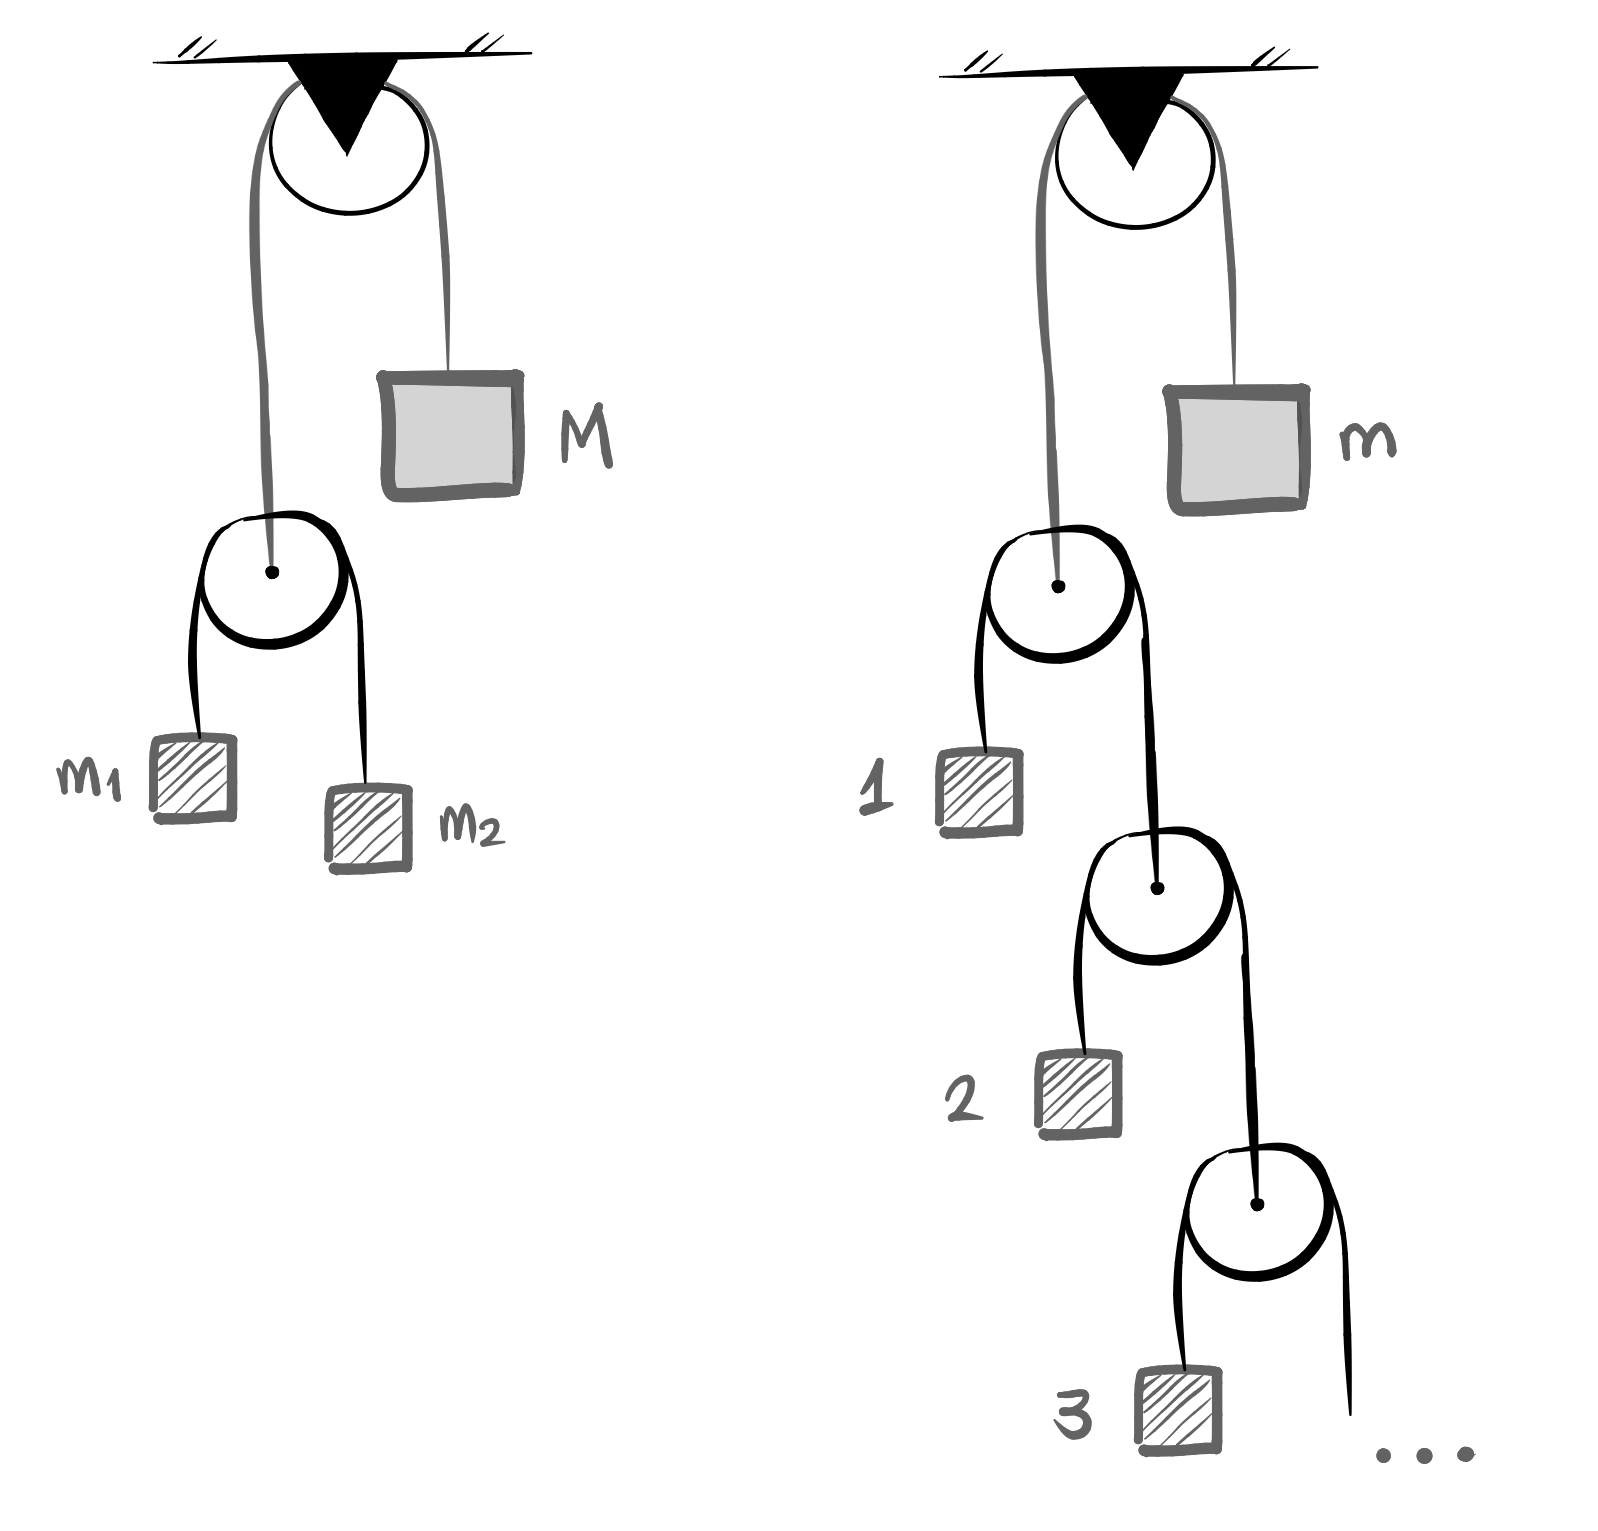
\includegraphics[width=0.5\linewidth]{imagensdinamicanewton/poliamovelex03.png}
% \captionof{figure}{}
% \label{fig_mec_poliamovelexemplo3}
% } 

% \begin{enumerate}


% \item [a)] Considere a máquina de Atwood da primeira imagem da Figura \ref{fig_mec_poliamovelexemplo3}. Qual é o valor de massa $M$, em função de $m_1$ e $m_2,$ que mantêm o sistema em equilíbrio?

% \item [b)] Considere a máquina de Atwood infinita da segunda imagem da Figura \ref{fig_mec_poliamovelexemplo3}. Encontre a tração no fio que prende a polia fixa ao teto, dado que todas as caixas $1,2,3,...$ possuem massa $m.$

% \item [c)] Considere a máquina de Atwood infinita da segunda imagem da Figura \ref{fig_mec_poliamovelexemplo3}. Encontre a tração no fio que prende a polia fixa ao teto, dado que as massas das caixas caem pela metade a cada nova polia, ou seja, $m_1= \sfrac{m}{2}, m_2= \sfrac{m}{4}, m_3= \sfrac{m}{8}, \dots$

% \end{enumerate}
% \resolucao

% 181, 182 e 183 RB

% \end{exemplo}


% \vspace{0.3cm}




\begin{secnivel}[Força de Atrito Estático Máximo]{I}{Força de Atrito Estático Máximo}
  
  \eqLdois{exp}{eq_newton_fatestatico}{F_{\text{AT}_{\text{MAX}}}= \mu_{e} N}

\end{secnivel}







\secgfe{De onde vem}

A Equação \eqref{eq_newton_fatestatico} calcula o valor da força de atrito estático máximo. Antes de examiná-la com mais atenção, convém compreender a natureza da força de atrito de maneira mais ampla.

Primeiro, vamos discorrer sobre sua origem. A força de atrito entre duas superfícies é uma força que irá resistir à tendência de movimento relativo entre as superfícies pelo fato de elas estarem, em escala microscópica, ``\textit{acopladas}.'' A Figura \ref{fig_mec_fatorigem} mostra essa situação, em que temos um bloco em equilíbrio em cima do solo. Ao observarmos a superfície de contato entre o bloco e o solo vemos que, diferente do que enxergamos a olho nu, tal superfície é repleta de irregularidades. 


\vspace{0.3cm}
{
\centering
\begin{tikzpicture}
  \begin{scope}[blend mode=multiply]
    \node {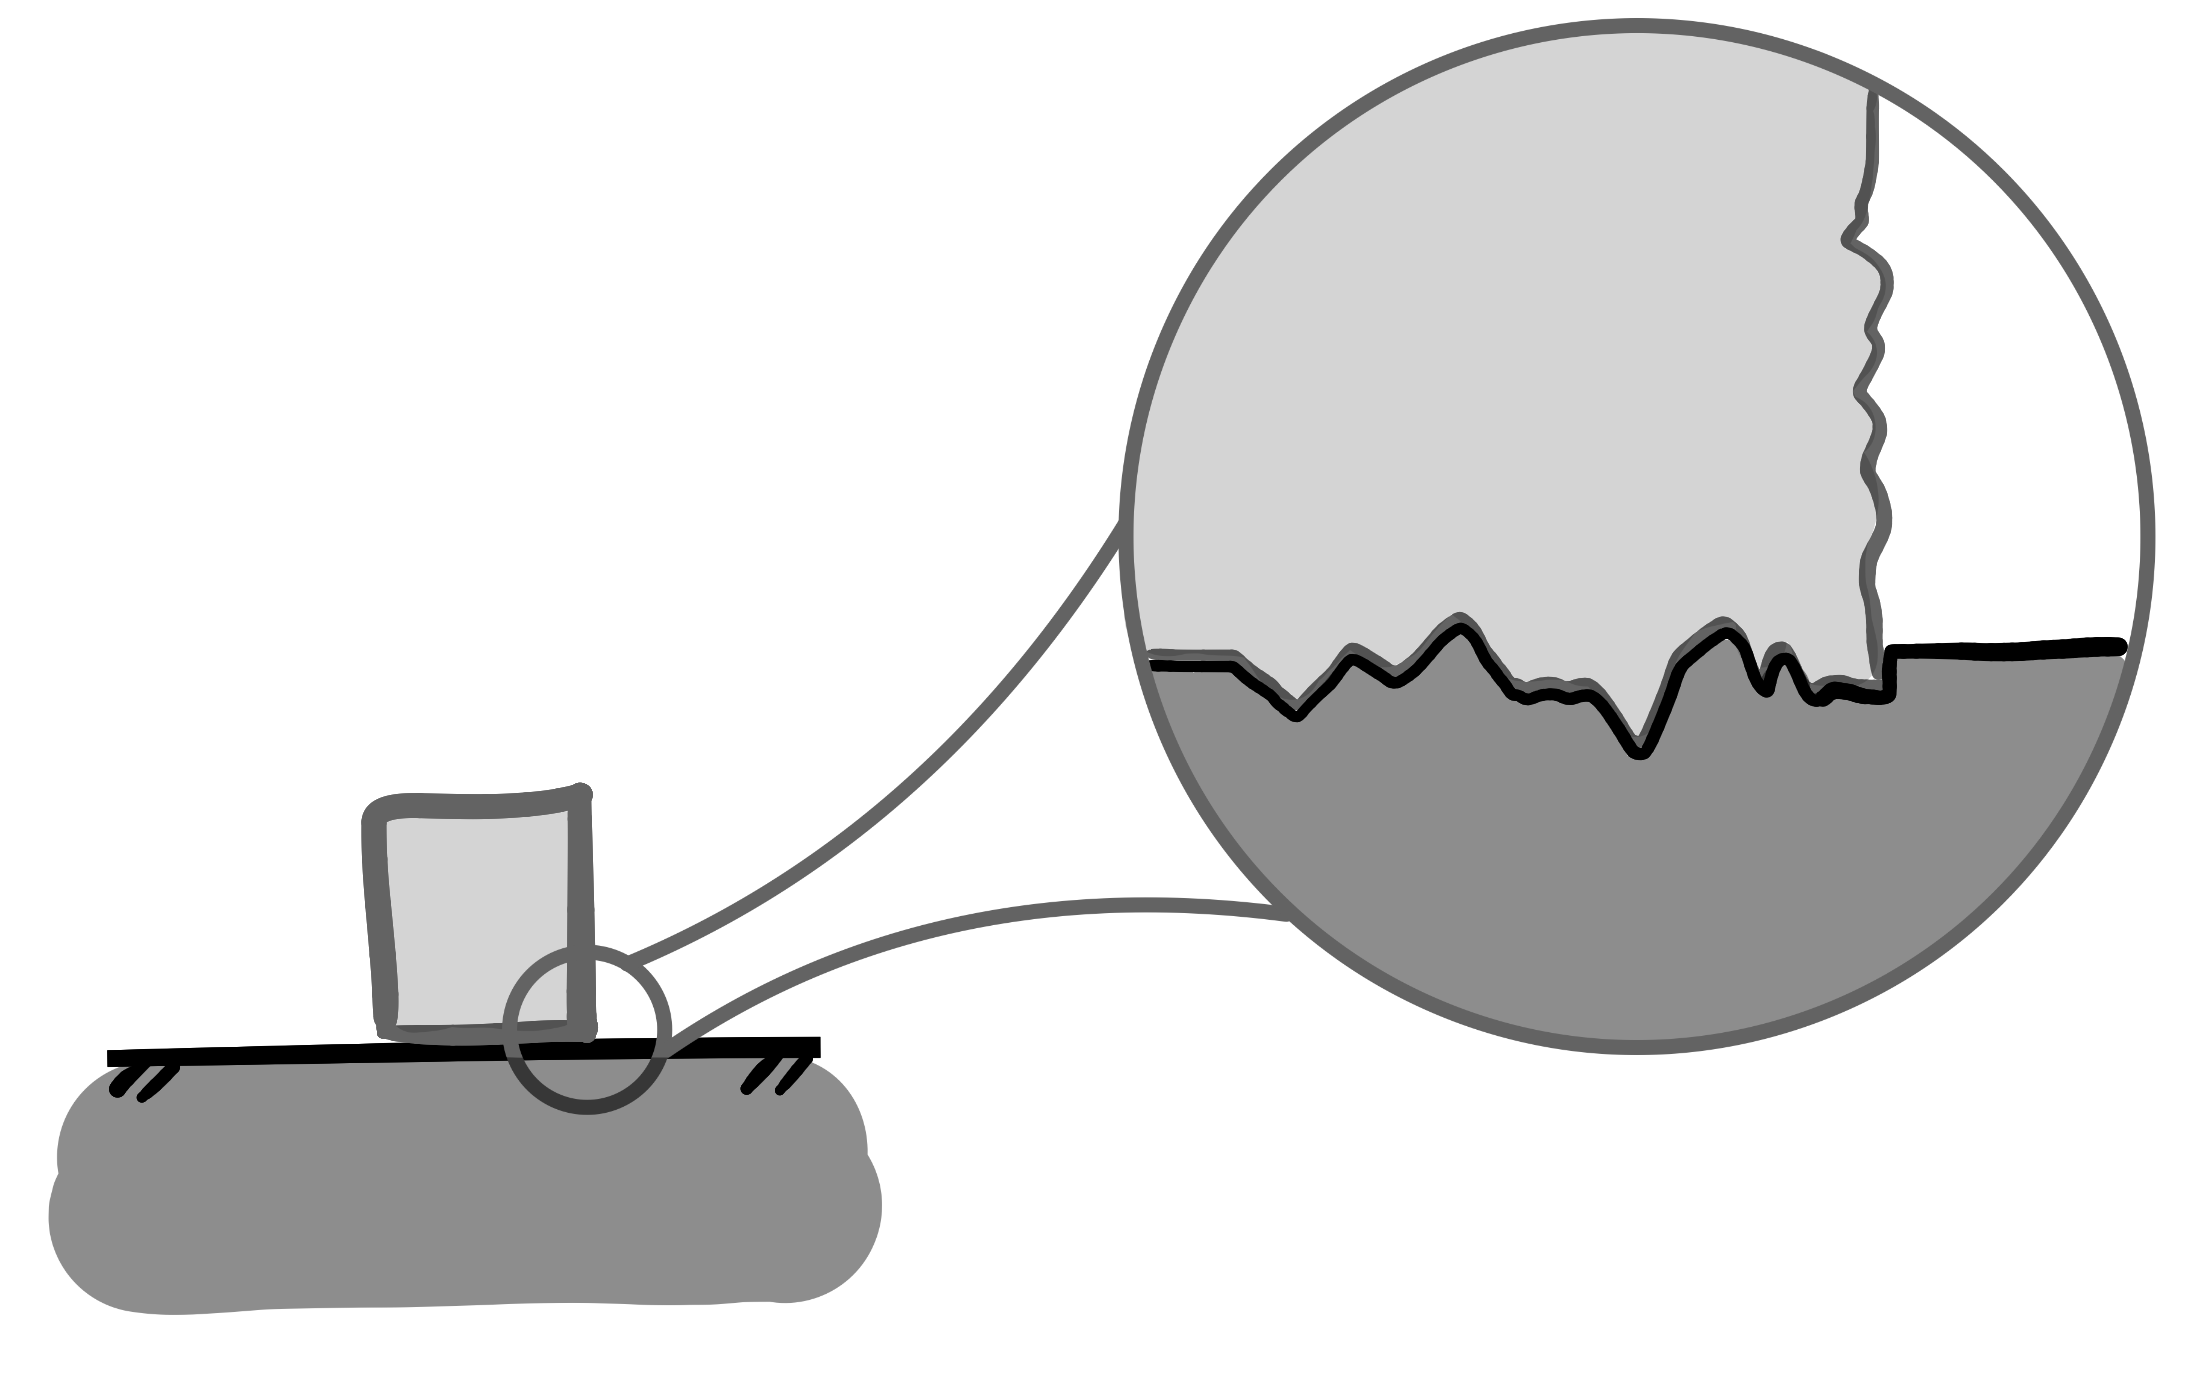
\includegraphics[width=0.4\linewidth]{imagensdinamicanewton/fatorigem.png}};
  \end{scope}
\end{tikzpicture}
\captionof{figure}{A origem da força de atrito.}
\label{fig_mec_fatorigem}
} 
\vspace{0.3cm}

Tais irregularidades se interpenetram, fazendo com que o bloco fique, de certo modo, fincado no solo, como se fossem raízes de um árvore. Assim, ao tentar movê-lo, encontraremos certa resistência para tal movimento. Essa resistência não existiria caso as superfícies fossem totalmente lisas, sem nenhuma irregularidade. Por isso, polir e lixar uma superfície (que é um tentativa de eliminar as irregularidades e deixá-la mais lisa) é uma forma de diminuir o atrito.




Em segundo lugar, sendo o atrito uma força, sabemos que se trata de uma grandeza vetorial, que possui, portanto, módulo, direção e sentido. Tratemos agora da sua direção e sentido. Estando a superfície do bloco da Figura \ref{fig_mec_fatorigem} ``\textit{fincada}'' no chão, é natural perceber que a força de atrito que se manifestará será paralela a tal superfície de contato; isto é, ela será, nesse caso, horizontal.

Isso porque, ao tentar empurrar o bloco, digamos, para a direita, as saliências e irregularidades do bloco penetradas na superfície do solo irão empurrar o solo para a direita. Assim, o solo reage e faz uma força para a esquerda no bloco. As forças trocadas, portanto, possuem sempre a direção da superfície de contato (sempre paralela ao plano, podendo ser para a direita ou para a esquerda).

Agora que já sabemos sobre a direção da força de atrito, vamos ao seu sentido: ela é sempre contrária à \textbf{tendência de movimento}. Essa é uma nuance que costuma gerar muitos erros. Note que ela exige um certo nível de abstração, uma vez que o bloco pode sequer se mover: é preciso imaginar, dadas as forças aplicadas nele, para onde ele \textbf{tende a se mover.} No caso de empurrar para a direita o bloco da Figura \ref{fig_mec_fatorigem}, a tendência é que ele se mova para a direita. Logo, o atrito, contrariando essa tendência, atua no bloco para a esquerda (isso se dá pela Terceira Lei de Newton, como construímos no raciocínio do parágrafo anterior). Perceba que, ao empurrar o bloco para a direita, pode ser que ele continue parado. Ou seja, ele sequer se move: o atrito estático é suficiente para mantê-lo em repouso e seria necessária uma força maior para colocá-lo em movimento. Sendo assim, é preciso sempre estar atento à tendência de movimento. O movimento em si pouco importa -- pode ser que ele sequer ocorra.

Na Figura \ref{fig_mec_fatcontratendenciamov} ilustramos diversos casos para que o leitor se familiarize com tal conceito. O primeiro caso é exatamente aquele da Figura \ref{fig_mec_fatorigem}, então dispensaremos sua análise. 

No segundo caso, ao empurrar o bloco de baixo pra direita com uma força $F$, sua tendência é se mover para a direita, naturalmente. Logo, o bloco de cima, por inércia, tende a ficar parado. Contudo, ficar parado em relação a um corpo que se move para a direita significa ficar para trás em relação a ele, ou seja, escorregar para a esquerda. Como a tendência do bloco de cima é escorregar para a esquerda em relação ao bloco de baixo, a força de atrito entre os blocos,\footnote{Analisamos aqui só as forças de atrito entre os blocos. Poderia haver também atrito entre o bloco maior e o chão. Neste caso, seria a mesma situação da primeira imagem da figura: o atrito atuaria para a esquerda.} contrariando tal tendência de movimento, atua para a direita, como mostra a imagem.

Na terceira situação da Figura \ref{fig_mec_fatcontratendenciamov} colocamos um bloco sob um plano inclinado, em repouso. Sua tendência, naturalmente, é escorregar plano abaixo. Logo, o atrito, contrário à tendência de movimento, atua na direção do plano, apontando para cima.

\vspace{0.3cm}
{
\centering
\begin{tikzpicture}
  \begin{scope}[blend mode=multiply]
    \node {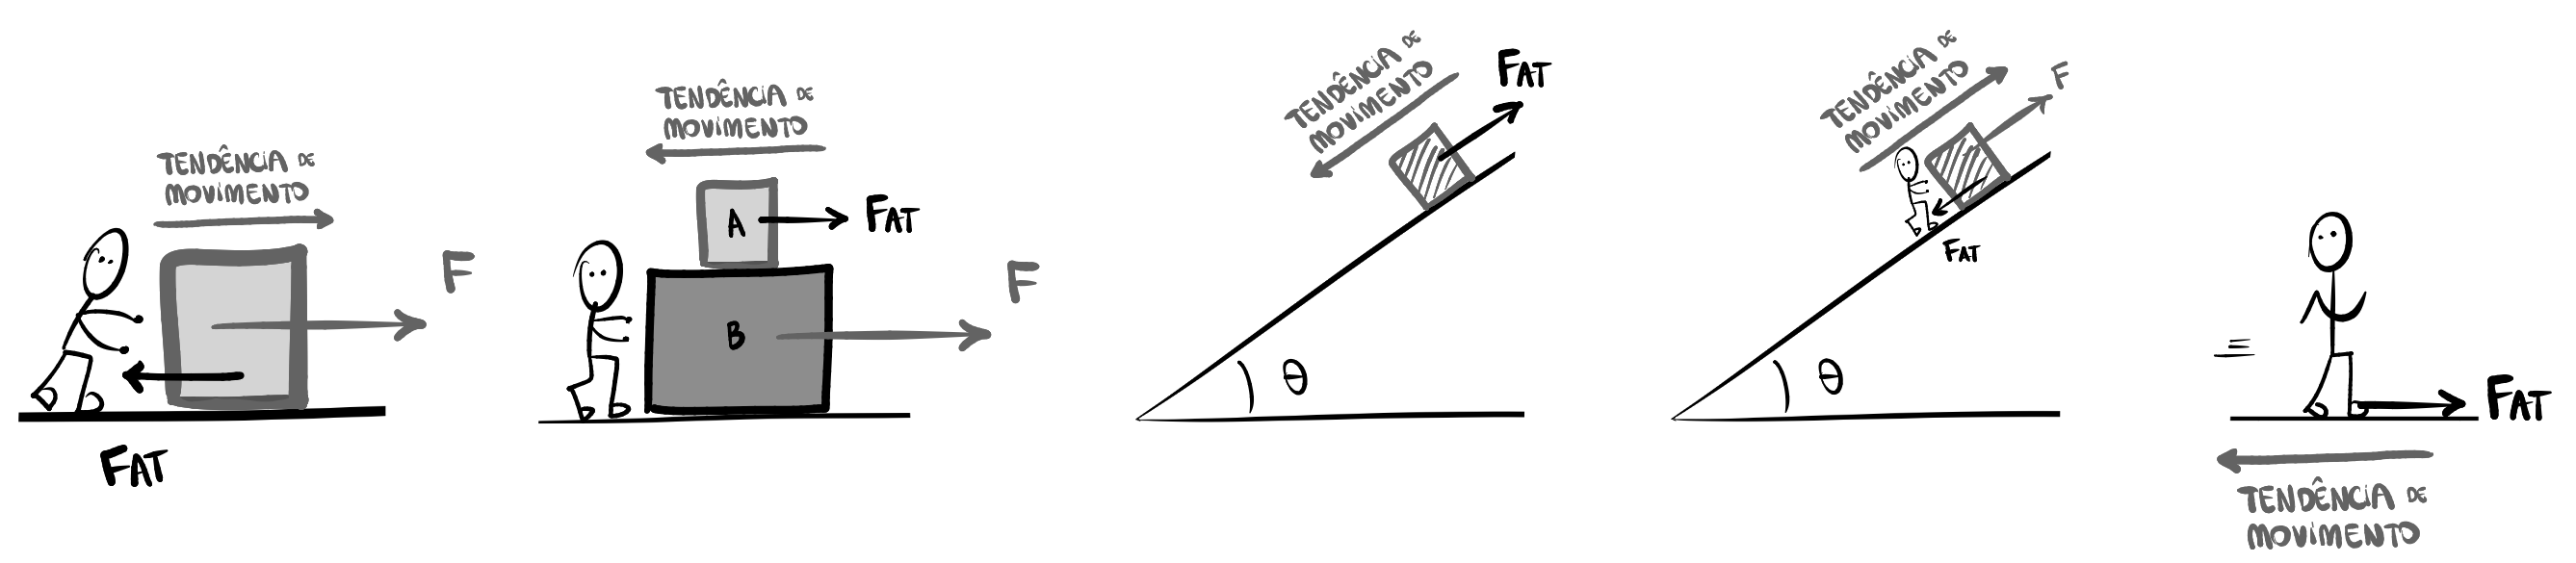
\includegraphics[width=1.0\linewidth]{imagensdinamicanewton/fatcontratendenciamov.png}};
  \end{scope}
\end{tikzpicture}
\captionof{figure}{A força de atrito é sempre paralela à superfície de contato entre os corpos e sempre se opõe à tendência de movimento.}
\label{fig_mec_fatcontratendenciamov}
} 
\vspace{0.3cm}

Já a quarta situação ilustra um contexto semelhante, porém agora um menino está empurrando o bloco com uma força tal que ele está quase começando a se mover plano acima. Assim, identificamos que a tendência de movimento do bloco é subir plano acima e o atrito, portanto, ao contrariar tal tendência de movimento, atua plano abaixo. Veja que curioso: na mesma situação -- um bloco sob um plano inclinado -- o atrito pode atuar plano acima ou plano abaixo. Tudo irá depender de qual é a tendência de movimento do bloco.

A última situação ilustra um exemplo cotidiano: o ato de andar. Ao dar um passo, fazemos um movimento de ``empurrar o chão para trás.'' A tendência, portanto, é que nosso pé escorregue para trás\footnote{Faça esse movimento sob uma casca de banana ou uma pista de gelo e constate por si só}, logo, o atrito, contrariando a tendência de movimento, atua para frente. Perceba, portanto, que neste caso o atrito atua a favor do movimento. Alguns leitores podem se surpreender com isso em um primeiro problema, mas não há nada de estranho: a força de atrito sempre se opõe à tendência de movimento, e não ao movimento em si. Portanto, não há nada de incoerente em uma situação na qual o atrito atue na mesma direção e sentido que o movimento -- veremos diversas situações como essa, inclusive.\footnote{Com isso, destaca-se que o atrito, portanto, pode tanto acelerar quanto desacelerar um corpo.}

Neste último caso, é o atrito que possibilita que o indivíduo caminhe, e é por isso que em uma superfície com pouco atrito (como uma pista de gelo) é muito difícil caminhar.




Em terceiro e último lugar, tratemos sobre o módulo da força de atrito. É exatamente isso que a Equação \eqref{eq_newton_fatestatico} se propõe a calcular. Na verdade ela se propõe a calcular o módulo da força de atrito estático \textbf{máximo}. Como veremos em breve, a força de atrito estático possui módulo variável, admitindo um valor máximo, que é aquele dado pela Equação \eqref{eq_newton_fatestatico}.

Tal equação é obtida por meio de experimentos, mas podemos compreendê-la com facilidade à luz de alguns conceitos que já construímos. Lembre-se da origem da força de atrito: ela está relacionada às irregularidades e rugosidades dos materiais, que fazem com eles fiquem ``fincados'' um no outro. Ora, quanto mais comprimido o bloco da Figura \ref{fig_mec_fatorigem} estiver contra o solo, mais ``fincado'' no solo ele estará e, consequentemente, maior será a força de atrito. Aqui, lembramos o leitor quem é o ente responsável por medir o quão comprimidas duas superfícies estão uma contra a outra: a força normal. 

A força normal é justamente definida como sendo a força de compressão entre duas superfícies em contato, sendo perpendicular a tal superfície de contato. Logo, é por isso que ela aparece na Equação \eqref{eq_newton_fatestatico}: a força de atrito é diretamente proporcional à compressão entre as superfícies: a força normal.

O termo $\mu_e$ é o chamado coeficiente de atrito estático, e é o termo que está relacionado ao quanto às superfícies em questão conseguem se acoplar. Trata-se de uma grandeza adimensional, em geral com valor entre 0 e 1, e é um valor obtido experimentalmente.

Digamos, por exemplo, que, por meio de experimentos, identifica-se que o coeficiente de atrito estático entre a madeira e o concreto é $\mu_e = 0.6.$ Se polirmos bem tais superfícies e, quem sabe, a lubrificarmos, conseguiremos diminuir o atrito, de modo que o coeficiente de atrito estático agora seria, digamos, $\mu_e = 0.3.$ Perceba, portanto, que tal coeficiente mede o quão bem as duas superfícies irão se acoplar: se polirmos as superfícies e diminuirmos suas irregularidades, o coeficiente de atrito diminui. Na chuva, como a estrada fica mais escorregadia, o coeficiente de atrito entre os pneus e o asfalto é menor do que no caso em que o asfalto está seco, por isso a estrada fica mais perigosa.


\secgfe{Onde é usada}

Como a Equação \eqref{eq_newton_fatestatico} calcula o valor da força de atrito estático máximo, isto é, o maior valor que a força de atrito pode assumir, ela é usada em geral em problemas nos quais um corpo se encontra na \textbf{iminência de se mover.} Ou seja, o corpo está sendo segurado pela força de atrito, mas está quase rompendo sua situação de equilíbrio: isso quer dizer que o atrito estático está assumindo o maior valor que pode. Daí em e diante ele não será capaz de segurar mais o bloco em equilíbrio.

\vspace{0.3cm}
{
\centering
\begin{tikzpicture}
  \begin{scope}[blend mode=multiply]
    \node {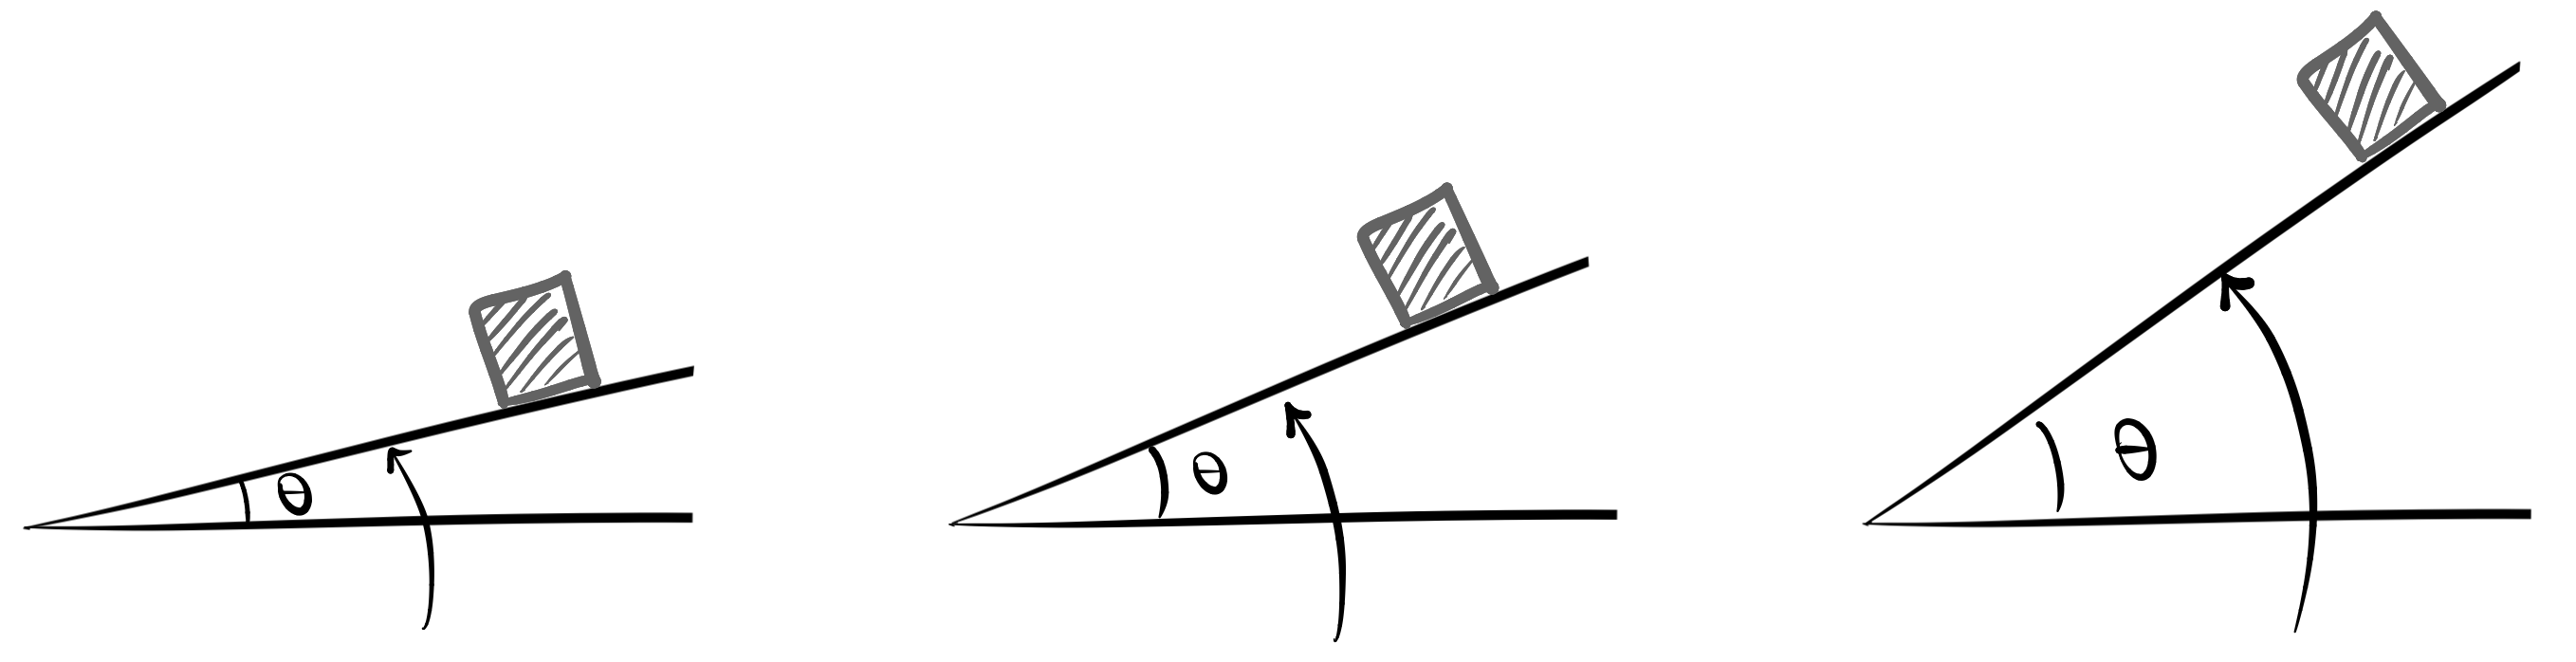
\includegraphics[width=0.8\linewidth]{imagensdinamicanewton/angulodeatrito1.png}};
  \end{scope}
\end{tikzpicture}
\captionof{figure}{}
\label{fig_mec_anguloatrito01}
} 

Para ilustrar isso, considere o experimento da Figura \ref{fig_mec_anguloatrito01}, em que um bloco está em equilíbrio sob um plano inclinado. O experimento consiste em ir aumentando gradativamente a inclinação do plano, até que o bloco se encontre na iminência de escorregar. Neste ponto, teremos inclinado tanto o plano de modo que o atrito está no seu limite: ele quase não consegue mais segurar o bloco em repouso. Essa é a situação em que a força de atrito estático assume seu valor máximo, que é justamente o contexto da Equação \eqref{eq_newton_fatestatico}.

\vspace{0.3cm}
{
\centering
\begin{tikzpicture}
  \begin{scope}[blend mode=multiply]
    \node {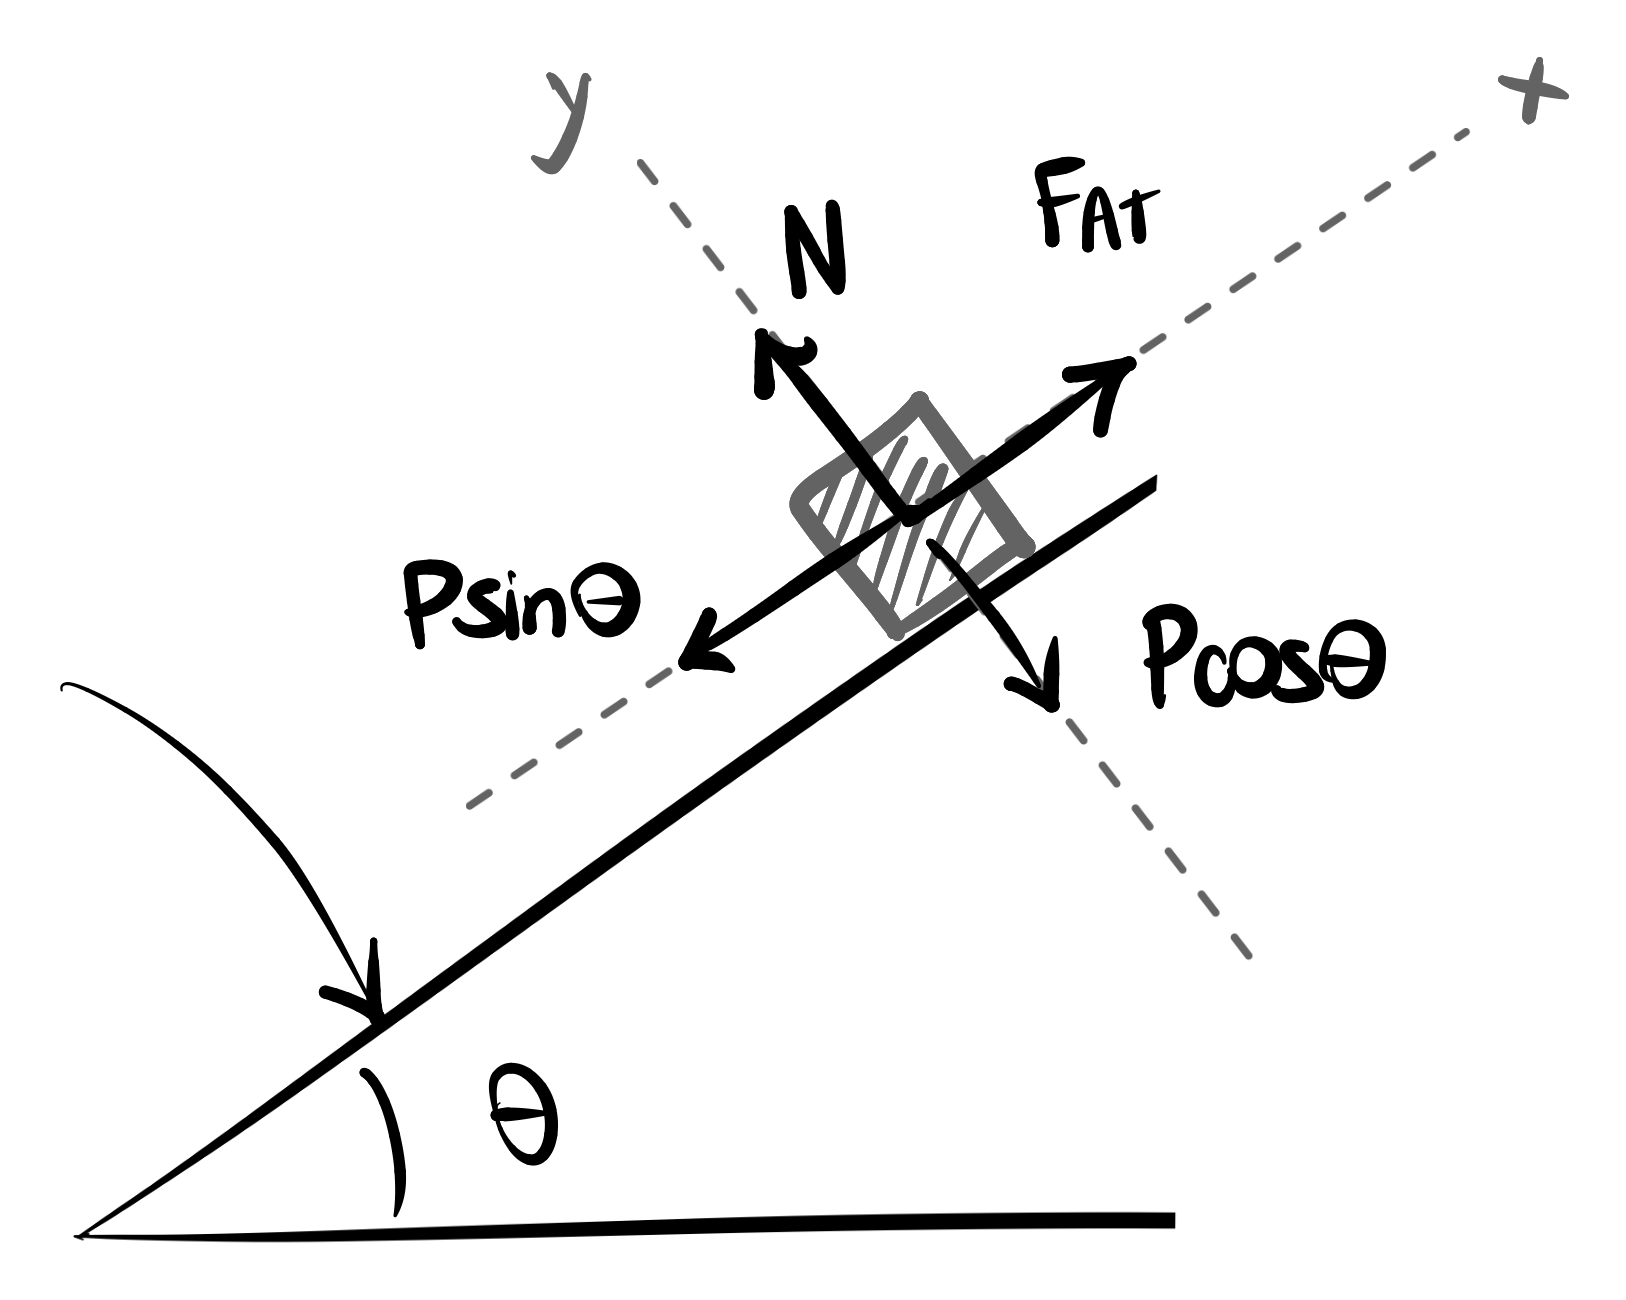
\includegraphics[width=0.3\linewidth]{imagensdinamicanewton/angulodeatrito2.png}};
  \end{scope}
\end{tikzpicture}
\captionof{figure}{}
\label{fig_mec_anguloatrito02}
} 
\vspace{0.3cm}

Essa situação está representada na última imagem da figura. O diagrama de forças de tal situação está representado na Figura \ref{fig_mec_anguloatrito02}, em que a força peso já foi representada decomposta nos eixos tangencial e normal, exatamente como feito para construir a Equação \eqref{eq_dinamicanewtoniana_gsintheta}. Do equilíbrio do bloco temos:


 \[
 \vec{F}_R = 0
\quad \xrightarrow{\text{projeção nos eixos}}
\quad
\begin{cases}
F_x = 0 \implies P \sin \theta = F_{\text{AT}_{\text{MAX}}} \\
F_y = 0 \implies P \cos \theta = N
\end{cases}
\] 

Usando a Equação \eqref{eq_newton_fatestatico} e as duas relações acima teremos:

$$ F_{\text{AT}_{\text{MAX}}} = \mu_e N \implies P \sin \theta = \mu_e P \cos \theta \implies \boxed{\mu_e = \tan \theta.} $$

O ângulo $\theta$ dado pela expressão acima é chamado de \textbf{ângulo de atrito:} sua tangente fornece justamente o coeficiente de atrito entre as superfícies do plano e do bloco.



Tal experimento é usado justamente para se determinar o coeficiente de atrito estático entre duas dadas superfícies. Por meio do cálculo da tangente do ângulo de atrito -- e o ângulo de inclinação do plano que deixa o bloco na iminência de movimento -- obtém-se o coeficiente de atrito estático.

\secgfe{Erros comuns}

O erro mais comum ao usar a Equação \eqref{eq_newton_fatestatico} é na sua interpretação: tal equação não fornece o valor da força de atrito estático, mas sim o da \textbf{força de atrito estático máximo.} Observe a Figura \ref{fig_mec_fatestaticovariavel} para entender essa diferença. 

Ao tentar empurrar o bloco, o menino começa fazendo uma força horizontal $F=20$N. Ele constata que o bloco, que estava inicialmente parado, permanece parado. Logo, a resultante das forças que nele atua permanece sendo nula, de onde conclui-se que o atrito estático respondeu com uma força cujo módulo vale, também, $20$N. 

Ao aumentar a força do empurrão para tentar tirar o bloco do lugar o menino faz uma força de $50$N, tão logo isso acontece ele constata que tal esforço foi insuficiente: o bloco continua em equilíbrio estático. Logo, conclui-se que o atrito estático respondeu com uma força cujo módulo vale, também, $50$N. E por aí vaí: ao empurrar o bloco com uma força de 55N o atrito responde com 55N, mantendo o bloco em repouso. Isso ocorre para diversos valores de força: o atrito sempre consegue igualar a força feita pelo menino, mantendo o bloco em repouso. Quer dizer, isso ocorre...até certo ponto.


\vspace{0.3cm}
{
\centering
\begin{tikzpicture}
  \begin{scope}[blend mode=multiply]
    \node {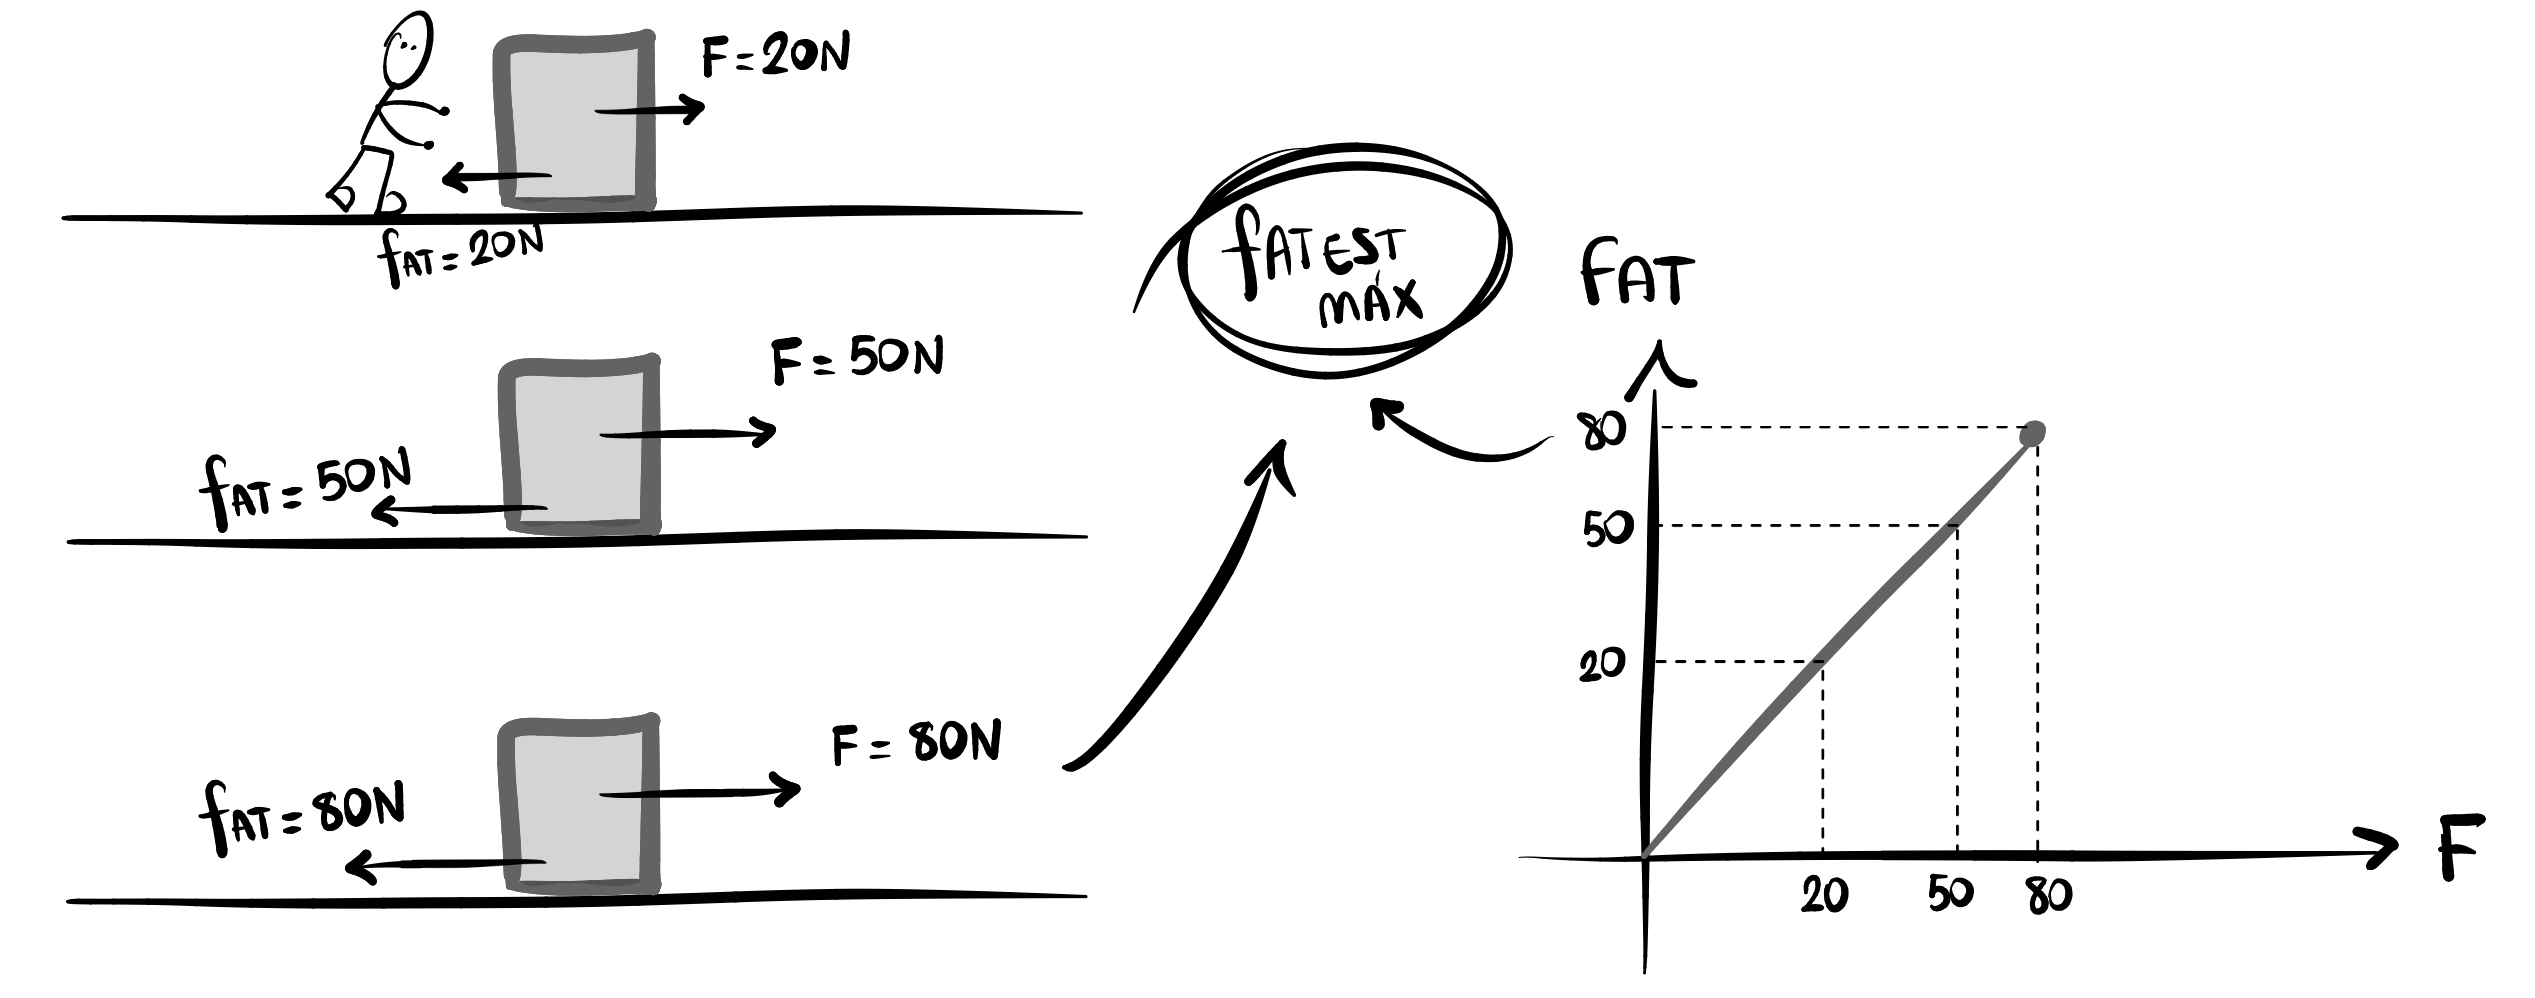
\includegraphics[width=0.8\linewidth]{imagensdinamicanewton/fatestaticovariavel.png}};
  \end{scope}
\end{tikzpicture}
\captionof{figure}{A força de atrito estático possui módulo variável, se igualando à força que a opõe, até um valor máximo.}
\label{fig_mec_fatestaticovariavel}
} 
\vspace{0.3cm}

Ao fazer uma força de $80$N o menino constata que está quase obtendo êxito em sua empreitada: o bloco está quase movendo, mais um cabelímetro\footnote{Um cabelímetro corresponde, aproximadamente, à espessura de um fio de
cabelo humano --- algo em torno de $70\,\mu$m, a depender da hidratação do autor
no dia da medição. Trata-se de uma unidade não reconhecida pelo Sistema Internacional
de Unidades, pelo Bureau Internacional de Pesos e Medidas, nem pela vizinha do autor,
que consultada a respeito manifestou indiferença. Sua principal vantagem em relação
ao micrômetro é fonética: ninguém nunca precisou soletrar cabelímetro duas vezes.} de força deve ser suficiente para tirá-lo do lugar. Essa condição é justamente a de iminência de movimento: o bloco está quase rompendo o equilíbrio estático, o atrito está quase deixando de ser capaz de mantê-lo em repouso. A essa força de atrito damos o nome de \textbf{força de atrito estático máxima,} e é ela que a Equação \eqref{eq_newton_fatestatico} se propõe a calcular.

Perceba, portanto, que a força de atrito estático tem módulo variável, como indica o próprio gráfico da Figura \ref{fig_mec_fatestaticovariavel}, que plota os dados da situação do menino empurrando o bloco. Porém, ela admite um valor máximo -- que corresponde à situação limite em que o repouso entre o bloco e a superfície do chão será mantido. Ao empurrar o bloco com uma força que seja um milésimo maior do que $80$N o bloco romperá seu equilíbrio e começará a se mover: o menino logrou êxito em sua tarefa. 

Daí em diante, ao começar a se mover, o atrito que atuará será o cinético, dado pela Equação \eqref{eq_newton_fatcinetico}, e será estudado na sequência.

Assim, caso o leitor prefira, é possível ler a Equação \eqref{eq_newton_fatestatico} como uma desigualdade: ela impõe um limite superior para a força de atrito estático, isto é:

$$ F_{AT} \leq \mu_{e} N. $$

O gráfico da Figura \ref{fig_mec_fatestaticovariavel} deixa isso evidente: a força de atrito estático pode assumir quaisquer valores, desde que sejam menores (ou igual) a $\mu_e N,$ que é o seu valor máximo.

\secgfe{Observações}

Acredito que cabem duas observações importantes a respeito da Equação \eqref{eq_newton_fatestatico}. A primeira delas é sobre o coeficiente de atrito $\mu_e$:

\begin{enumerate}
    \item ele é uma grandeza adimensional: é uma razão entre duas forças, a força de atrito e a força normal, e, portanto, não possui unidade de medida.

    \item  o coeficiente de atrito não é uma propriedade intrínseca do corpo, é algo que depende das duas superfícies que estão em contato. O coeficiente de atrito entre uma caixa de madeira e uma superfície de metal será, em geral, diferente do coeficiente de atrito entre a mesma caixa de madeira uma superfície de madeira, por exemplo.
\end{enumerate}


A segunda observação é sobre o movimento relativo. Ao ler a Equação \eqref{eq_newton_fatestatico}, por se tratar do atrito estático, o leitor pode ser levado a crer que tal equação se aplica só se o bloco estiver parado. Isso até está correto...contudo, o que significa estar parado? Como vimos na construção da Equação \eqref{mecanica_eq_velocidaderelativa}, um corpo parado em um referencial pode muito bem -- e em geral estará -- estar se movendo em relação a outro.

Dito isso, o termo estático que caracteriza tal atrito está relacionado ao movimento relativo entre as duas superfícies que estão em contato no contexto. Se um bloco está sob uma superfície horizontal, o atrito atuante será estático caso a superfície do bloco não se mova \textbf{em relação ao chão} (ela pode muito bem estar se movendo em relação a algum outro observador). Considere, por exemplo, a situação da Figura \ref{fig_mec_atritoestaticomovendo1}.

\vspace{0.3cm}
{
\centering
\begin{tikzpicture}
  \begin{scope}[blend mode=multiply]
    \node {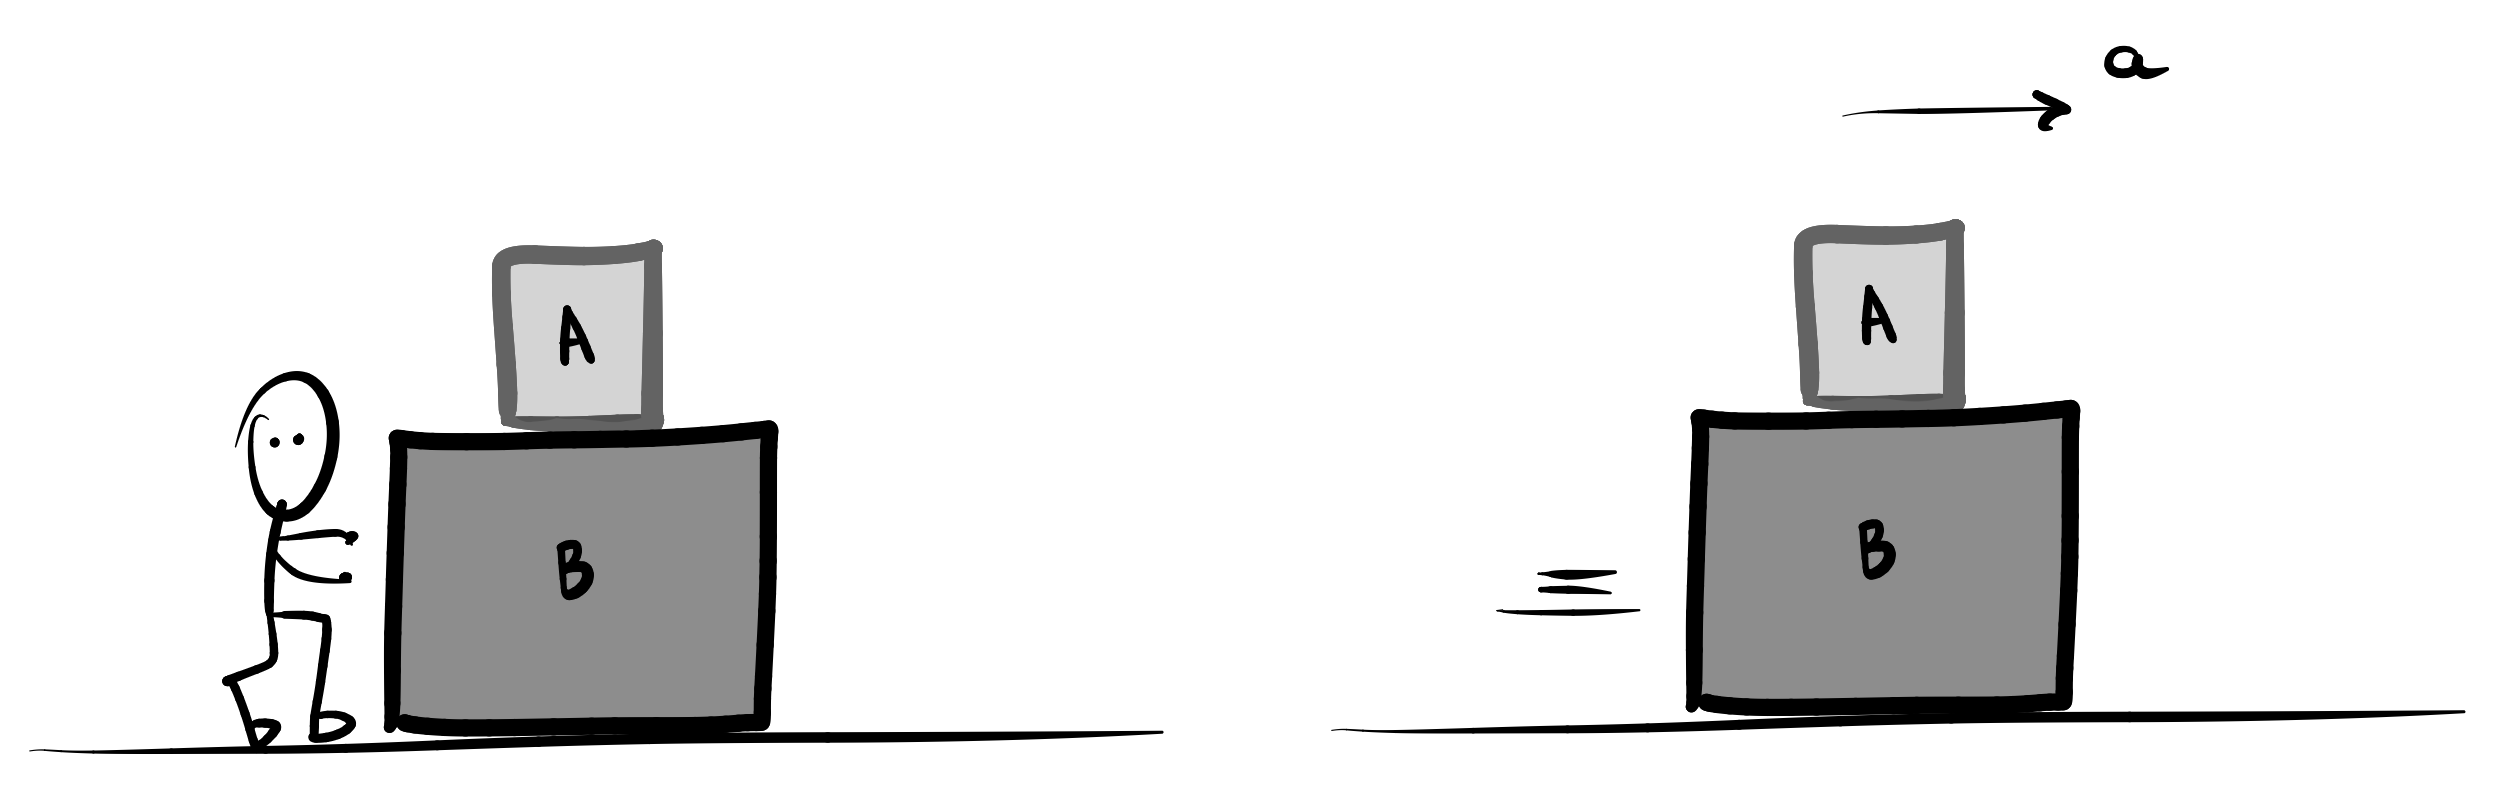
\includegraphics[width=0.7\linewidth]{imagensdinamicanewton/atritoestaticomovendo1.png}};
  \end{scope}
\end{tikzpicture}
\captionof{figure}{Quando os dois blocos aceleram juntos, sem que $A$ escorregue em relação a $B,$ então eles possuem exatamente a mesma aceleração e $A$ está em repouso em relação a B.}
\label{fig_mec_atritoestaticomovendo1}
} 
\vspace{0.3cm}

A situação mostra um pequeno bloco, de massa $m$, apoiado em cima de um outro bloco maior, de massa $M.$ Este, por sua vez, está apoiado no chão. Um indivíduo empurra o bloco de baixo e consegue imprimir uma aceleração $a$ no sistema, que se move de tal sorte que o bloco de cima não se move em relação ao bloco debaixo.

Não seria espantoso que um espírito ainda não calejado na solução de uma grande diversidade de problemas de física imaginasse, com certa confiança prematura, que, como os blocos se movem, o atrito que atua entre eles não poderia ser estático.

Isso certamente está errado pois, como bem lembramos, o adjetivo estático em questão se refere à superfície de contato entre os corpos. Se observarmos bem, o contexto do problema nos diz que os blocos se movem juntos, sem que um escorregue em relação ao outro. Isso quer dizer que eles se movem -- em relação à Terra -- exatamente com a mesma aceleração e, portanto, estão em repouso um em relação ao outro.




Poderíamos, inclusive, computar qual deve ser a máxima aceleração $a$ a se imprimir neste sistema tal que essa situação seja possível. Para isso, considere que o coeficiente de atrito estático entre os blocos $A$ e $B$ é $\mu_e$. A Figura \ref{fig_mec_atritoestaticomovendo2} mostra o diagrama de forças nos dois blocos. 

Sobre as forças no bloco $A$ temos: 

\begin{enumerate}
    \item  A força $N_{BA}$ é a normal feita pelo bloco $B$ no bloco $A$ -- sua reação é $N_{AB}$, de mesmo módulo, e atua no bloco B.
     \item  A força $F_{AT_{BA}}$ é a força de atrito feita pelo bloco $B$ no bloco $A$: como, ao empurrar o bloco $B$ para direita, a sua tendência é se mover para a direita, enquanto o bloco $A$ ficaria parado, vemos que a tendência de $A$ seria escorregar para a esquerda em relação a $B.$ A força de atrito, contrariando essa tendência de movimento, se manifesta para a direita. Sua reação é $F_{AT_{AB}}$ e atua no bloco B. 
     \item A força peso $P=mg$, vertical para baixo.
\end{enumerate}

\vspace{0.3cm}
{
\centering
\begin{tikzpicture}
  \begin{scope}[blend mode=multiply]
    \node {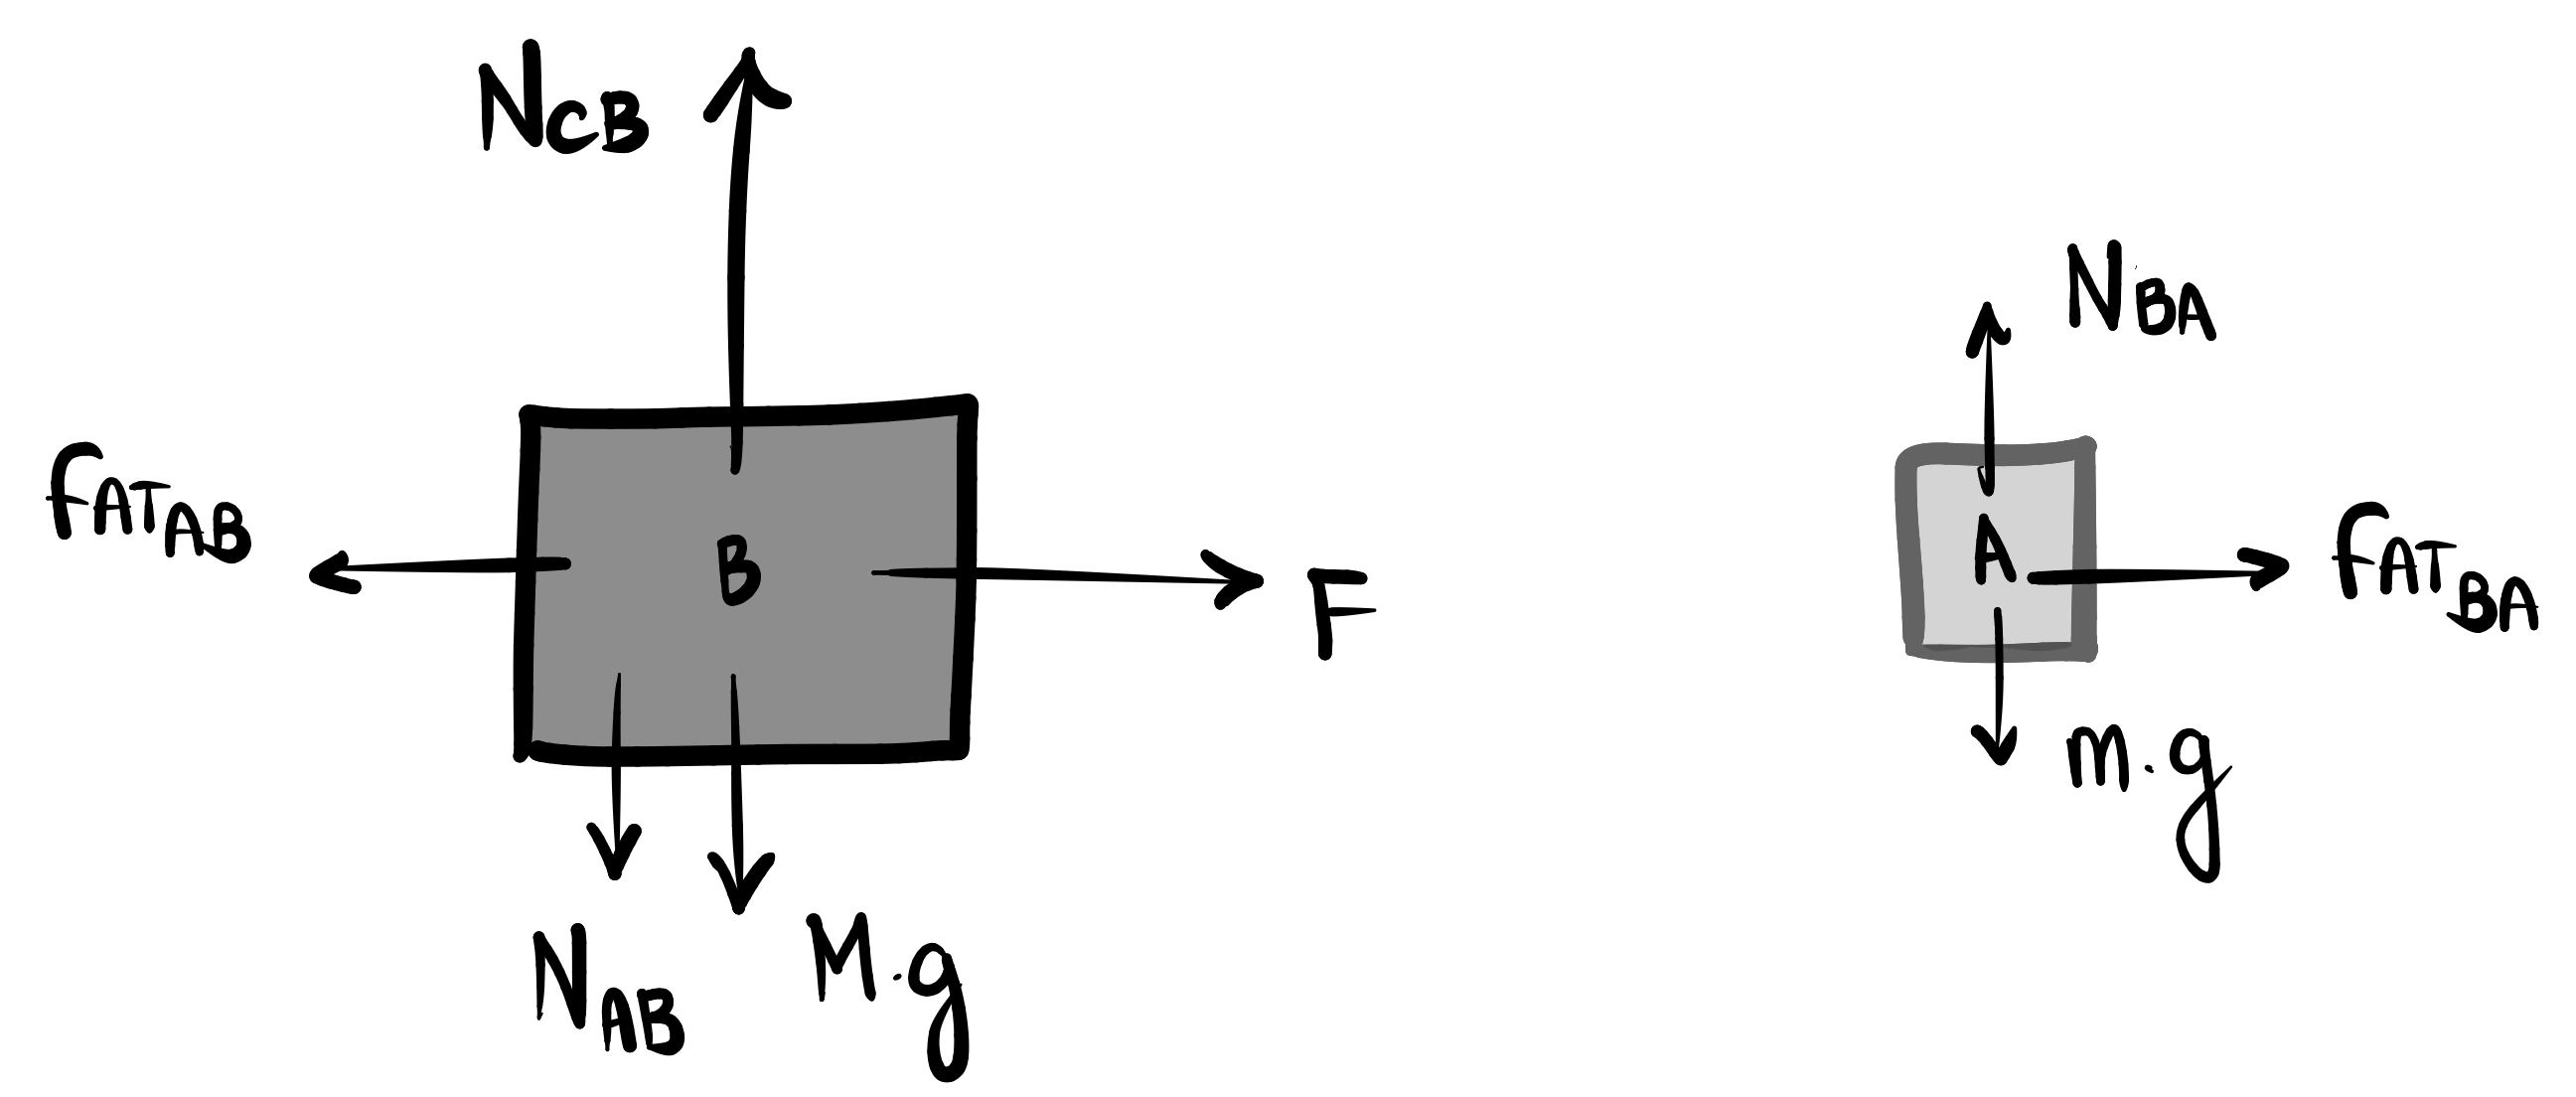
\includegraphics[width=0.6\linewidth]{imagensdinamicanewton/atritoestaticomovendo2.png}};
  \end{scope}
\end{tikzpicture}
\captionof{figure}{Análise das forças que atuam nos blocos que se movem com a mesma aceleração horizontal $a.$}
\label{fig_mec_atritoestaticomovendo2}
} 
\vspace{0.3cm}

Como o bloquinho não se move na vertical, há equilíbrio nessa direção:

$$ F_{Ry} = 0 \implies N_{BA} = mg.$$

Já na horizontal a resultante das forças tem que ser capaz de gerar no bloquinho a mesma aceleração $a$ para a direita que o bloco maior possui, para que eles estejam em repouso relativo:

$$ F_{Rx} = ma \implies F_{AT_{AB}} = ma.$$

Usando as duas equações acima na desigualdade $F_{AT} \leq \mu_e N$ temos

$$ ma \leq \mu_e mg \implies \boxed{a \leq \mu_e g, }$$

\noindent ou seja, o maior valor possível de aceleração para que tal situação seja possível é $a_\text{max}= \mu_e g.$

Para acelerações superiores a essa o atrito estático não conseguirá segurar o bloquinho em repouso em relação ao bloco maior e ele começará a escorregar para a esquerda em relação a tal bloco. Note como tal relação faz sentido: 

\begin{enumerate}
    \item [(i)] a aceleração máxima é proporcional a $\mu_e$. Isso quer dizer que, quanto maior o coeficiente de atrito, maior pode ser a aceleração máxima que o sistema pode ter de modo que os blocos não escorreguem um em relação ao outro. Isso faz total sentido, haja vista que é o próprio atrito quem está impedindo que haja movimento relativo entre os blocos, e $\mu_e$ é justamente o número que mede o quão acoplados os blocos estão.

    \item [(ii)] além disso, a aceleração máxima também é proporcional à gravidade. Isso ocorre porque, quanto mais intensa for a gravidade, maior será o ``\textit{acoplamento}'' entre os dois blocos, uma vez que maior será a força (peso) que puxa um bloco contra o outro (ou seja, a normal será maior). Em um local de menor gravidade os blocos estão menos ``\textit{grudados}'' um com o outro e, portanto, a aceleração máxima que o sistema pode ter para que os blocos permaneçam em repouso relativo é menor.
\end{enumerate}







Por fim, representamos também na Figura \ref{fig_mec_atritoestaticomovendo2}, a título de deixar completa a análise, as forças no bloco $B.$ Elas são desnecessárias para a análise deste problema, mas, para o leitor mais curioso, são elas: $N_{CB}$ é a normal trocada entre o bloco $B$ e o chão. Sua reação tem o mesmo módulo e atua no chão. $F$ seria a força feita pelo menino no bloco, $Mg$ é o peso do bloco e as demais forças já foram discutidas.

\vspace{0.3cm}

\begin{exemplo}[Nível I]\label{exemplo_newton_fatestatico01}

Um bloco de massa $m$ é comprimido contra uma parede vertical, como mostra a Figura \ref{fig_mec_fatestaticoex011} por uma força $F.$ O atrito entre a parede vertical e o bloco é tal que o coeficiente de atrito vale $\mu.$ 

\vspace{0.3cm}
{
\centering
\begin{tikzpicture}
  \begin{scope}[blend mode=multiply]
    \node {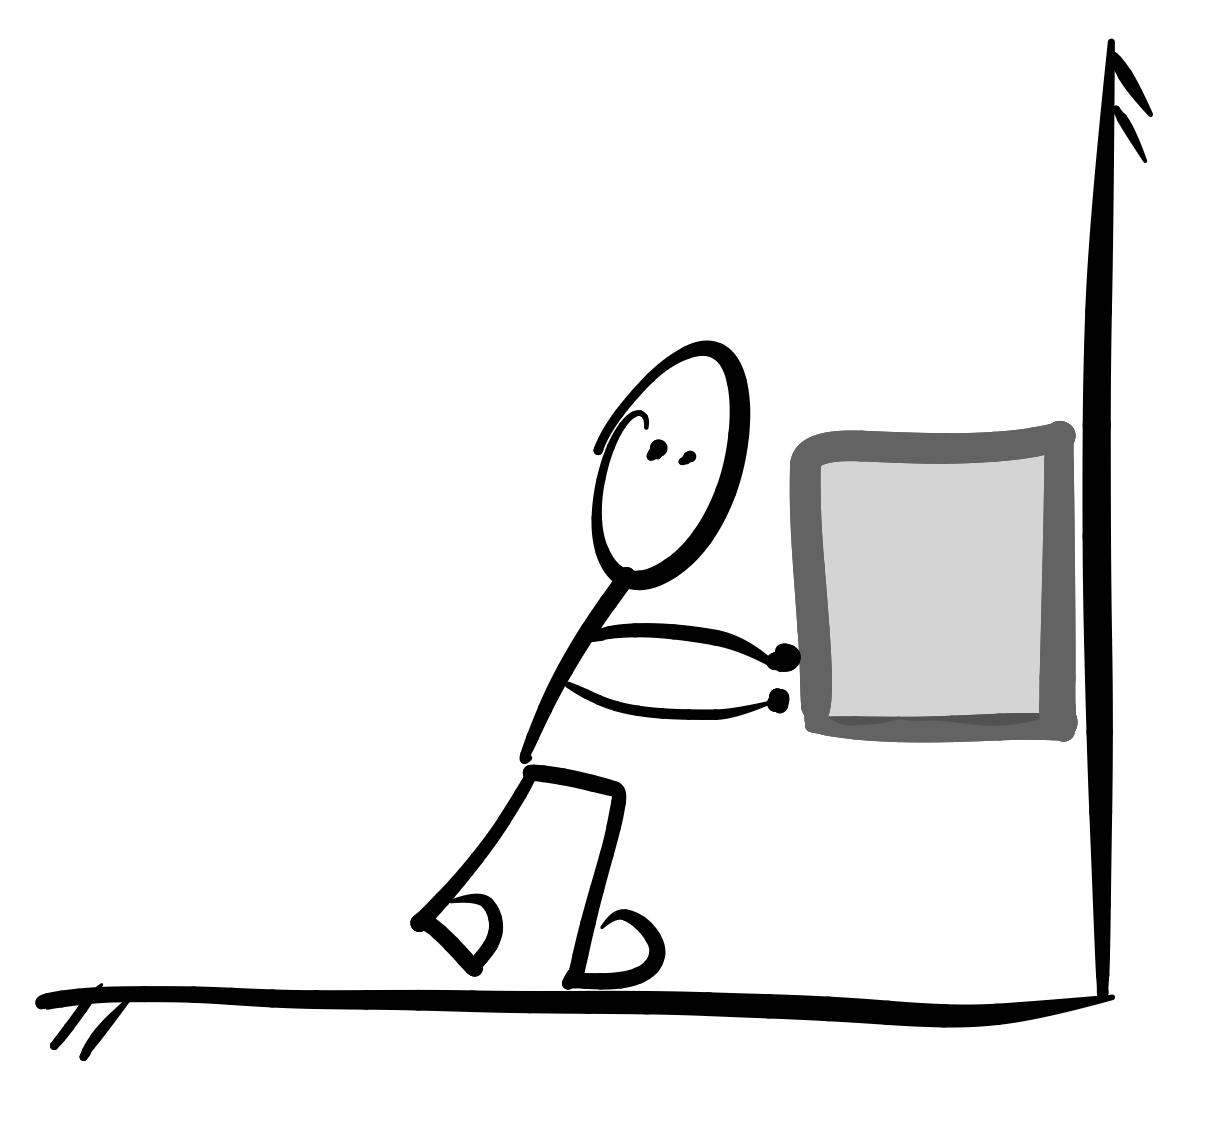
\includegraphics[width=0.25\linewidth]{imagensdinamicanewton/fatestaticoex011.png}};
  \end{scope}
\end{tikzpicture}
\captionof{figure}{}
\label{fig_mec_fatestaticoex011}
} 
\vspace{0.3cm}



Se a gravidade local vale $g$, calcule a menor força $F$ que deve ser feita no bloco para que ele fique em equilíbrio quando

\begin{itemize}
    \item [a)] $m=2$ kg e $\mu_e = 0.5.$
    \item [b)] $m=10$ kg e $\mu_e=0.5.$
    \item [c)] $m=10$ kg e $\mu_e=0.8.$
    \item [d)] $m$ e $\mu$ quaisquer.
\end{itemize}


\resolucao

Como queremos o bloco em equilíbrio, para as situações dos quatro itens trabalharemos no regime de atrito estático, e o diagrama de forças no bloco será aquele da Figura \ref{fig_mec_fatestaticoex012}. 

O menino faz uma força $F,$ horizontal para a direita, comprimindo o bloco contra a parede. Com isso, o bloco empurra a parede para a direita com uma força normal $N$, e, pela Terceira Lei de Newton, a parede faz uma força $N$ para a esquerda no bloco. A figura também representa seu peso $P=mg,$ que atua verticalmente para baixo. Como a tendência do bloco é escorregar parede abaixo, o atrito, contrariando tal tendência, atua para cima.

\vspace{0.3cm}
{
\centering
\begin{tikzpicture}
  \begin{scope}[blend mode=multiply]
    \node {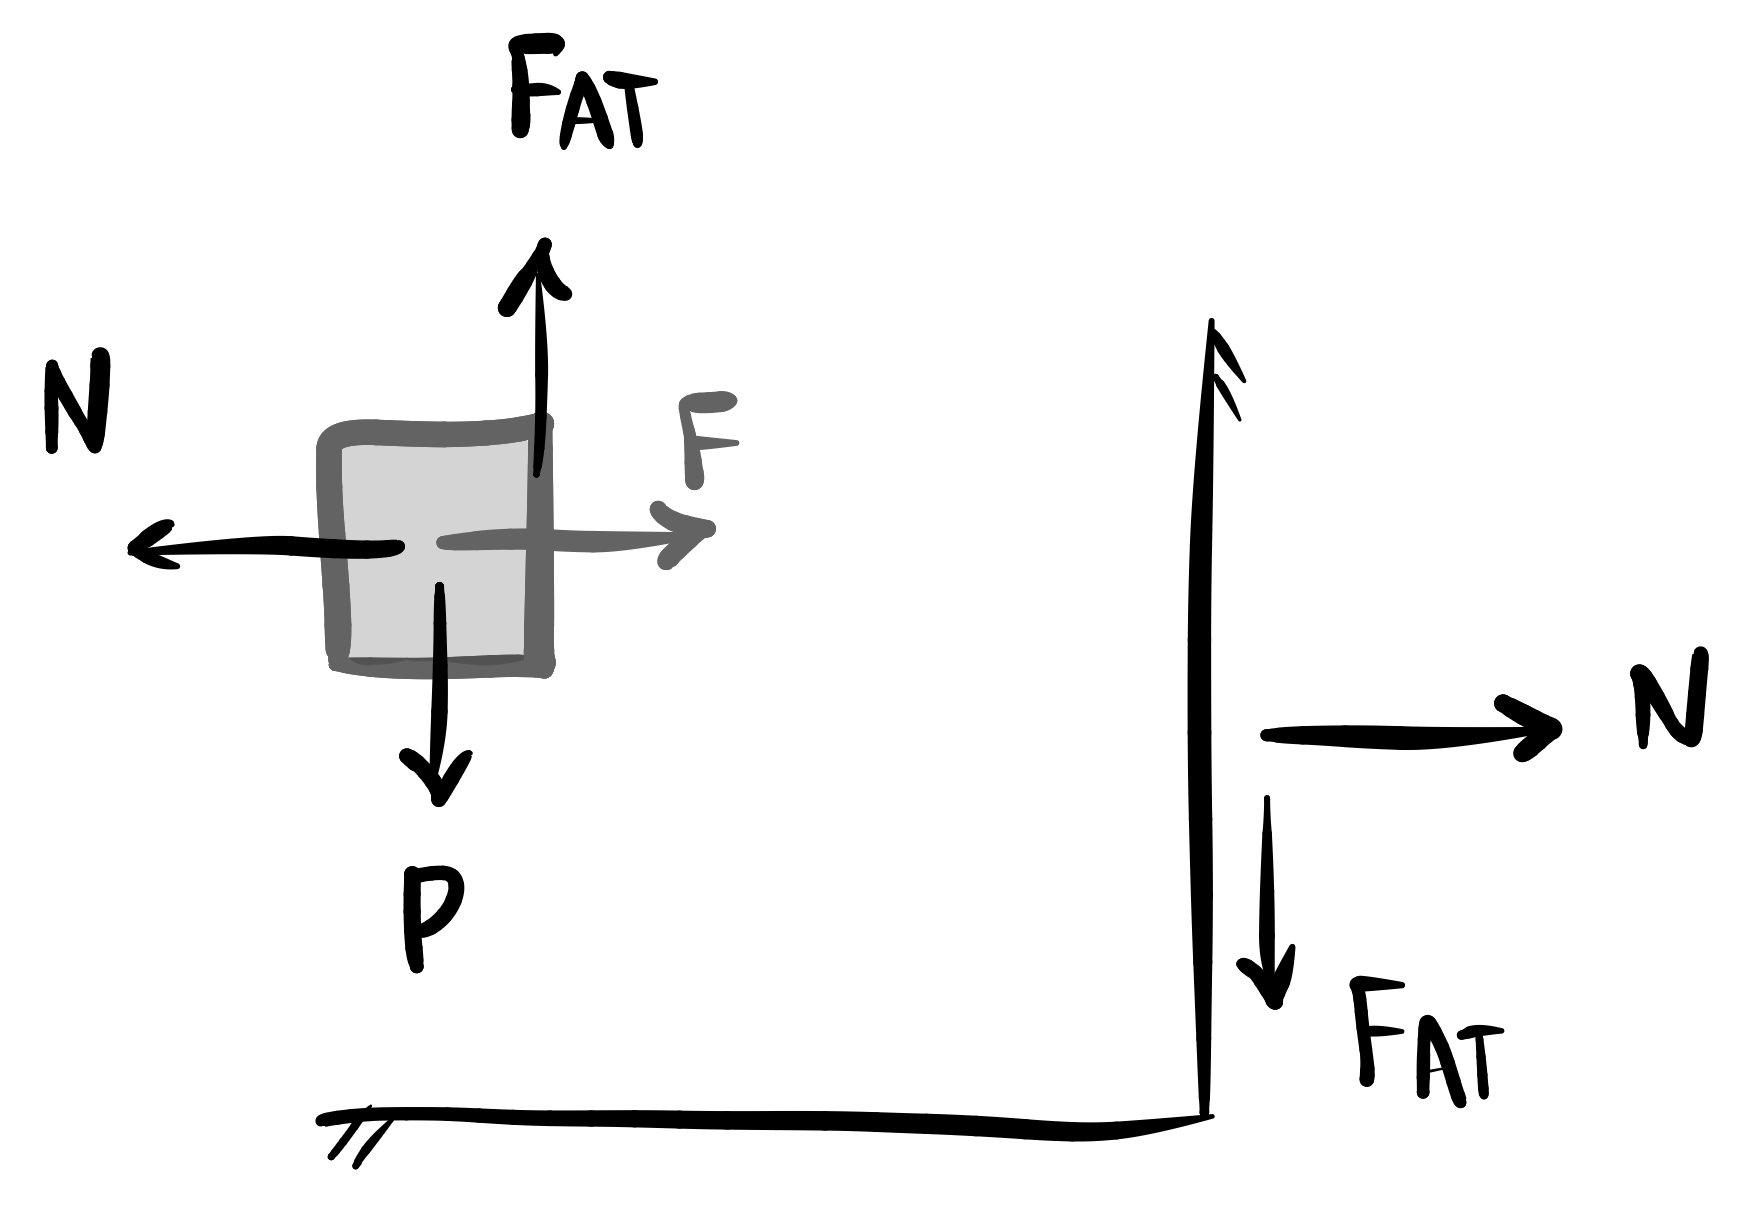
\includegraphics[width=0.3\linewidth]{imagensdinamicanewton/fatestaticoex012.png}};
  \end{scope}
\end{tikzpicture}
\captionof{figure}{Diagrama de forças no bloco e reações na parede.}
\label{fig_mec_fatestaticoex012}
} 
\vspace{0.3cm}

Vamos analisar agora cada situação:


\begin{itemize}
    \item [a)] $m=2$ kg e $\mu = 0.5.$

    Neste caso o peso é $P=mg = 20$N. Na horizontal as forças vão se anular, haja vista o equilíbrio do bloco. Logo, teremos que $N=F.$

    Sabemos que $F_{\text{AT}} \leq \mu_e N$, logo:


    $$ F_{\text{AT}} \leq \mu_e F \implies F \geq \dfrac{F_{\text{AT}}}{\mu_e},  $$


   \noindent contudo, sabemos também que precisamos ter -- do equilíbrio vertical do bloco -- $F_\text{AT}=P=20$N, logo

   $$  F \geq \dfrac{F_{\text{AT}}}{\mu_e} \implies F \geq \dfrac{20}{0.5} \implies \boxed{F \geq 40 \text{ N.}} $$

   Ou seja, a menor força $F$ com que se deve empurrar o bloco contra a parede para que ele não escorregue e fique em equilíbrio é de 40N.
    
    \item [b)] $m=10$ kg e $\mu=0.5.$


    O raciocínio aqui é idêntico ao anterior, só mudando o valor do peso $P$ do bloco, que trocaremos de 20N para 100N:

    $$  F \geq \dfrac{F_{\text{AT}}}{\mu_e} \implies F \geq \dfrac{100}{0.5} \implies \boxed{F \geq 200 \text{ N.}} $$

    Ou seja, a menor força $F$ com que se deve empurrar o bloco contra a parede para que ele não escorregue e fique em equiíbrio é de 200N. Como temos o mesmo coeficiente de atrito e um bloco mais pesado, é natural esperar que tenhamos que comprimi-lo com mais intensidade contra a parede para mantê-lo em equilíbrio. \footnote{Perceba a física do problema: já intui-se que, para manter um bloco mais pesado em repouso dessa forma será necessário comprimi-lo com ainda mais intensidade contra a parede vertical. De fato isso ocorre, porque quanto maior é a intensidade com que se empurra o bloco contra a parede (força $F),$ maior é a compressão do bloco contra a parede (força normal $N$ e, como sabemos, o atrito entre duas superfícies é proporcional ao quanto elas estão comprimidas uma contra a outra -- força normal). Assim, quanto mais intenso for a força $F$ que comprime o bloco na parede, maior será o atrito capaz de segurar o bloco de escorregar para baixo.}
    
    \item [c)] $m=10$ kg e $\mu=0.8.$

     O raciocínio aqui é idêntico ao anterior, só mudando o valor do coeficiente de atrito, que foi usado apenas no último passo do cálculo:

    $$  F \geq \dfrac{F_{\text{AT}}}{\mu_e} \implies F \geq \dfrac{100}{0.8} \implies \boxed{F \geq 125 \text{ N.}} $$

    
      Ou seja, a menor força $F$ com que se deve empurrar o bloco contra a parede para que ele não escorregue e fique em equiíbrio é de 125N. Como o coeficiente de atrito é maior, a normal também pode ser menor para que se gere o mesmo atrito capaz de sustentar o peso do bloco.
    
    \item [d)] $m$ e $\mu$ quaisquer.

      Usando que $F_{\text{AT}} = P=mg$ e a desigualdade $ F \geq \dfrac{F_{\text{AT}}}{\mu_e} $, chegamos em

      $$ F \geq \dfrac{mg}{\mu_e}. $$


       Ou seja, quanto maior o valor de massa $m$ maior é a força $F$ horizontal necessária para gerar atrito suficiente de modo que o bloco fique em repouso, como esperávamos. Além disso, quanto maior o coeficiente de atrito estático $\mu_e,$ menor é o valor de tal força, como também era esperado.
    
\end{itemize}





\end{exemplo}


\vspace{0.3cm}


\begin{exemplo}[Nível II]\label{exemplo_newton_fatestatico02}

Considere um trem e um bloco de massa $m$, colocado na sua dianteira. Se a gravidade é vertical e seu módulo vale $g$ e o coeficiente de atrito estático entre o bloco e o vagão vale $\mu,$ qual é a menor aceleração $a$ que o trem deve ter para que ele consiga se mover sem que o bloco escorregue em relação a ele?

\vspace{0.3cm}
{
\centering
\begin{tikzpicture}
  \begin{scope}[blend mode=multiply]
    \node {\includegraphics[width=0.6\linewidth]{imagensdinamicanewton/fatvagaoetrem1.png}};
  \end{scope}
\end{tikzpicture}
\captionof{figure}{}
\label{fig_mec_fatvagaoetrem1}
} 


\resolucao

Avaliemos as forças no bloco de massa $m$. Temos o seu peso, atuando verticalmente para baixo. A normal $N$ de compressão entre o bloco e a parede vertical do vagão, sempre perpendicular à superfície de contato. E, temos também a força de atrito $F_{\text{AT}}$, que atua para cima, uma vez que a tendência do bloco é escorregar para baixo (por conta da gravidade).

\vspace{0.3cm}
{
\centering
\begin{tikzpicture}
  \begin{scope}[blend mode=multiply]
    \node {\includegraphics[width=0.6\linewidth]{imagensdinamicanewton/fatvagaoetrem2.png}};
  \end{scope}
\end{tikzpicture}
\captionof{figure}{Diagrama de forças da situação.}
\label{fig_mec_fatvagaoetrem2}
} 
\vspace{0.3cm}

Se o bloco não se move em relação ao vagão isso significa que

\begin{enumerate}
    \item [(i)] O bloco não se move na vertical, uma vez que o vagão não possui movimento vertical. Logo, as forças no bloco se equilibram na vertical: $F_{\text{AT}}=P=mg.$

    \item [(ii)] O bloco compartilha exatamente do mesmo movimento que o vagão na horizontal, isto é, ele se move horizontalmente com a mesma aceleração $a$ do vagão:

    $$ F_{\text{Rx}} = ma \implies N = ma.$$

    Assim, garantimos que o bloco não se move em relação ao vagão.
\end{enumerate}

Inserindo os dois resultados acima na desigualdade $F_{\text{AT}} \leq \mu_e N$ somos levados a

 $$ mg \leq \mu_e ma \implies \boxed{a \geq \dfrac{g}{\mu_e} .}$$

 Ou seja, a menor aceleração a ser imprimida no vagão de modo que a caixa fique \textit{grudada} nele e não escorregue é exatamente igual a $a = \sfrac{g}{\mu_e.}$ \footnote{Note que não é simples executar tal façanha, uma vez que para a quase totalidade dos casos teremos $0 < \mu_e < 1$. Logo, a aceleração horizontal que o vagão precisaria ter seria, em geral, maior do que a da gravidade. No caso em que $\mu_e = 0.5,$ por exemplo, seria necessário imprimir no vagão uma aceleração horizontal igual a $\sfrac{g}{0.5} = 2g$, ou seja, o dobro da aceleração da gravidade, o que é uma aceleração bastante alta. A título de comparação, a aceleração máxima de um carro comum gira em torno de 2 m/s$^2$ e 4 m/s$^2$.}

\end{exemplo}


\vspace{0.3cm}

\begin{exemplo}[Nível III]\label{exemplo_newton_fatestatico03}

A caixa de massa $M$ está apoiada sobre o solo, como mostra a Figura \ref{fig_mec_fatestaticoex03}. Sendo $\mu$ o coeficiente de atrito estático entre tais superfícies e $g$ a aceleração da gravidade, mostre que a menor força $F$ capaz de mover a caixa é aquela para o qual $\phi = \arctan (\mu).$


\vspace{0.3cm}
{
\centering
\begin{tikzpicture}
  \begin{scope}[blend mode=multiply]
    \node {\includegraphics[width=0.3\linewidth]{imagensdinamicanewton/fatestaticoex03.png}};
  \end{scope}
\end{tikzpicture}
\captionof{figure}{}
\label{fig_mec_fatestaticoex03}
} 
\vspace{0.3cm}


\resolucao


O equilíbrio de forças exige que 

$$ F_\text{R} = 0 \begin{cases}
    F_{\text{R}_x} = 0 \implies  F \cos \phi = F_\text{AT} \\
    F_{\text{R}_y} = 0 \implies  F \sin \phi + N = Mg \implies N= Mg - F \sin \phi 
\end{cases}$$

Se a caixa está quase se movendo, então estamos na condição de \emph{iminência de movimento,} e o atrito é o estático máximo:

$$ F_\text{AT} = \mu N \implies F \cos \phi =  \mu Mg - \mu F \sin \phi, $$

\noindent ou seja:

$$ F (\cos \phi + \mu \sin \phi) = \mu Mg \implies F = \dfrac{\mu Mg}{(\cos \phi + \mu \sin \phi).}$$

Procuramos encontrar a \emph{menor} força $F$ possível. Ora, note que $\mu$, $M$ e $g$ -- os termos que compõem o numerador da expressão acima -- são constantes. Logo, $F$ assume valores diferentes por conta dos diferentes ângulos $\phi$ com os quais ela pode ser feita, ou seja, temos uma força $F(\phi).$ Desse modo, quanto \emph{maior} for o denominador, menor será o valor de tal força. Assim, nosso problema se reduz a \emph{maximizar} o valor da expressão

$$ f(\phi) = \cos \phi + \mu \sin \phi.$$

Tal expressão pode ser reescrita como

$$ f(\phi) = \sqrt {\mu^2 +1} \left( \dfrac{1}{\sqrt {\mu^2 +1}}\cos \phi + \sin \phi \dfrac{\mu}{\sqrt {\mu^2 +1}} \right).$$

Note, contudo, pelo triângulo abaixo, que
$$ \sin \alpha = \dfrac{1}{\sqrt {\mu^2 +1}} \quad \text{ e } \quad \cos \alpha = \dfrac{\mu}{\sqrt {\mu^2 +1}}, $$

\noindent em que $\alpha$ é um ângulo fixo, dependente do fator $\mu$, dado por $\alpha = \arctan (\mu^{-1})$. Assim, a expressão de $f(\phi)$ pode ser reescrita como

$$ f(\phi) = \sqrt {\mu^2 +1}  \left( \sin \alpha \cos \phi + \sin \phi \cos \alpha    \right) \implies f(\phi) = \sqrt {\mu^2 +1} \sin (\phi + \alpha).$$

\vspace{0.3cm}

\begin{center}
    

\begin{tikzpicture}[scale=2]
    % Pontos (catetos com comprimentos próximos)
    \coordinate (A) at (0,0);
    \coordinate (B) at (1.2,0);
    \coordinate (C) at (1.2,1);

    % Triângulo
    \draw[thick] (A) -- (B) -- (C) -- cycle;

    % Ângulo reto em B
    \draw[thick] (1.05,0) -- (1.05,0.15) -- (1.2,0.15);

    % Ângulo alpha em A
    \draw[thick] (0.35,0) arc[start angle=0,end angle=40,radius=0.35];

    % Rótulos dos lados
    \node[below] at (0.6,0) {$\mu$};
    \node[right] at (1.2,0.5) {$1$};
    \node[above left] at (0.6,0.5) {$\sqrt{\mu^2+1}$};

    % Rótulo do ângulo alpha
    \node at (0.5,0.18) {$\alpha$};
\end{tikzpicture}


\end{center}






Ora, como dito, o ângulo $\alpha$ é um ângulo fixo, determinado de forma única pelo parâmetro $\mu.$ De toda forma, ainda que não o fosse, o fato é que $\sin (\phi+\alpha),$ quaisquer que sejam os valores de $\phi$ e $\alpha,$ é sempre uma expressão cujo máximo valor é 1:

$$ -1 \leq \sin (\phi+\alpha) \leq 1.$$

Desse modo, multiplicando a desigualdade por $\sqrt {\mu^2 +1}$, teremos:

$$ - \sqrt {\mu^2 +1} \leq f(\phi) \leq \sqrt {\mu^2 +1},$$

\noindent de onde vemos que o valor \emph{máximo} de $f(\phi)$ é $\sqrt {\mu^2 +1}$, o que ocorre quando o seno é um:

$$ \sin (\phi + \alpha) = 1 \implies \phi + \alpha = \dfrac{\pi}{2} \implies \phi = \dfrac{\pi}{2} - \alpha.$$

Logo, tem-se

$$ \tan (\phi) = \tan \left(\dfrac{\pi}{2} - \alpha \right) = \dfrac{1}{\tan (\alpha)} = \mu, $$

\noindent ou seja, $\phi = \arctan (\mu),$ como queríamos demonstrar.

Munidos do ângulo que fornece a força mínima, de $\tan \phi = \mu$ extraímos que $\sin \phi = \mu/\sqrt{1+\mu^2}$ e $\cos \phi = 1/\sqrt{1+\mu^2}$, de modo que a força mínima é


$$F (\phi)= \dfrac{\mu Mg}{(\cos \phi + \mu \sin \phi)} \implies \boxed{F_\text{MIN} = \dfrac{ Mg \mu\sqrt{1+\mu^2}}{1+\mu^2}.}$$


\end{exemplo}








\begin{secnivel}[Força de Atrito Cinético]{I}{Força de Atrito Cinético}
  
  \eqLdois{exp}{eq_newton_fatcinetico}{F_{\text{AT}_\text{C} }= \mu_{c} N}

\end{secnivel}






\secgfe{De onde vem}

Considere a situação da Figura \ref{fig_mec_fatestaticovariavel}. Constatamos que a força de $80$N era o maior valor de força que o atrito estático poderia fazer, mantendo, assim, o bloco em situação de equilíbrio estático. O que aconteceria se continuássemos a imprimir no bloco uma força $F$ maior que $80$N? Ora, naturalmente, ele entraria em movimento, e o atrito estático deixaria de existir.



O atrito, contudo, que possui origem nas imperfeições, rugosidades e saliências da estrutura da matéria, continuaria existindo, só mudaria de regime: a força de atrito que atua quando há movimento relativo entre as superfícies é o atrito cinético. O seu módulo, direção, sentido e sua origem são exatamente os mesmos daqueles discutido no desenvolvimento da Equação \eqref{eq_newton_fatestatico}.

Note que a estrutura da Equação \eqref{eq_newton_fatcinetico} é exatamente a mesma da Equação \eqref{eq_newton_fatestatico}, de modo que é natural compreendê-la à luz da discussão feita sobre o atrito estático. O que muda aqui são, essencialmente, duas coisas:

\begin{enumerate}
    \item [(i)] O coeficiente de atrito cinético, $\mu_c$, é, em geral, diferente do coeficiente de atrito estático. Experimentos mostram que 

    $$ \mu_e \geq \mu_c,$$

    \noindent ou seja, a força de atrito estático máxima é maior do que a força de atrito cinético. Isso é razoável de se compreender, uma vez que, no repouso, há maior intertravamento microscópico entre as superfícies. Já ao iniciar o movimento, essas ``\textit{ligações}'' são rompidas, fazendo com que o efeito do atrito seja menor.

    \item [(ii)] A força de atrito cinético é constante, e seu módulo é dado pela Equação \eqref{eq_newton_fatcinetico}. Diferente do atrito estático, que tem módulo variável e admite um valor máximo, o atrito cinético possui módulo constante. 
    
    Isso está indicado no gráfico da Figura \ref{fig_mec_fatcineticografico}: ao fazer sob o bloco uma força maior do que o atrito estático consegue igualar para mantê-lo em equilíbrio, o bloco começa a se mover. Tão logo isso ocorre, o atrito entra em regime cinético, de modo que seu valor cai (porque $\mu_e \geq \mu_c)$ e fica constante. No caso, para $40$N, mas tal valor é ilustrativo -- não há necessidade alguma da força de atrito cinético ser exatamente metade da força de atrito estático máxima.
\end{enumerate}



{
\centering
\begin{tikzpicture}
  \begin{scope}[blend mode=multiply]
    \node {\includegraphics[width=0.8\linewidth]{imagensdinamicanewton/fatcineticografico.png}};
  \end{scope}
\end{tikzpicture}
\captionof{figure}{O regime de atrito cinético e estático.}
\label{fig_mec_fatcineticografico}
} 
\vspace{0.3cm}




\secgfe{Onde é usada}

Basicamente em todo contexto em que dois corpos em contato possuem suas superfícies de contato em movimento relativo. 

Uma aplicação extremamente elegante da Física no cotidiano é o sistema de freios ABS (\textit{Anti-lock Braking System}). Para compreendê-lo corretamente, precisamos antes esclarecer uma ideia que costuma confundir muitos estudantes: \textit{por que o atrito entre o pneu e o solo é estático, se o carro está em movimento?}

Pois é. O leitor desatento poderia imaginar que, uma vez que o carro se move em relação ao chão, o atrito entre o solo e os pneus do carro seria o cinético. Mas, em geral, é o estático -- desde que não haja deslizamento (derrapagem).


Quando um carro se desloca com as rodas rolando sem deslizar, cada ponto do pneu descreve um movimento circular em torno do eixo da roda. No entanto, o ponto específico do pneu que está em contato com o solo possui, naquele instante, velocidade nula em relação ao chão. É como se o ponto do pneu em contato com o chão estivesse momentaneamente em repouso e toda a roda girasse em torno daquele ponto. \\



Logo, se o ponto do pneu em contato com o chão está em repouso instantâneo -- ou seja, é um rolamento sem deslizamento --, não há movimento relativo entre o pneu e o solo e, portanto, o atrito que atua é o estático.

Mas o que acontece quando a roda trava? Se o motorista freia bruscamente e a roda trava, ela para de girar. O carro continua avançando por inércia, mas agora o ponto de contato do pneu passa a deslizar sobre o asfalto: o carro começa a derrapar.

Nesse momento há movimento relativo entre as superfícies, de modo que o atrito deixa de ser estático e passa a atuar o \textbf{atrito cinético}. E aqui surge um ponto crucial da Física que já levantamos
\[
\mu_e > \mu_c,
\]

\noindent ou seja, o coeficiente de atrito estático é maior que o cinético. Isso significa que, quando a roda trava, a força de atrito disponível diminui -- entra no regime cinético. A frenagem fica menos eficiente, a distância de frenagem aumenta e o motorista perde controle direcional. 

Este seria o funcionamento de um carro sem freios ABS, e está ilustrado no primeiro gráfico da Figura \ref{fig_mec_fatcABS}, já conhecido por nós, em que a força $F$ aqui representaria a força com que o motorista pressiona os freios, que é o que vai gerar a compressão do disco de freio contra a roda do carro.

No carro sem freio ABS, inicialmente, a força de atrito ($F_{\text{AT}}$) cresce proporcionalmente à força aplicada ($F$). Ela se ajusta exatamente ao valor necessário para impedir o deslizamento. No gráfico, isso corresponde à reta crescente até o valor máximo (por exemplo, $80\,\text{N}$). Esse ponto representa o \textbf{atrito estático máximo}.

Se a força aplicada ultrapassa esse limite, ocorre o escorregamento. A força de atrito sofre uma queda abrupta para um valor menor. No gráfico, essa queda aparece como a passagem do ponto superior (por exemplo, $80\,\text{N}$) para um patamar inferior (por exemplo, $40\,\text{N}$). Esse patamar é aproximadamente constante, característica do atrito cinético.

\vspace{0.3cm}
{
\centering
\begin{tikzpicture}
  \begin{scope}[blend mode=multiply]
    \node {\includegraphics[width=0.8\linewidth]{imagensdinamicanewton/fatABS.png}};
  \end{scope}
\end{tikzpicture}
\captionof{figure}{O carro sem freio ABS (primeira imagem) e com freio ABS (segunda imagem).}
\label{fig_mec_fatcABS}
} 
\vspace{0.3cm}







Já o sistema de freios ABS impede que a roda permaneça travada. Sensores monitoram continuamente a rotação das rodas e modulam a pressão do freio diversas vezes por segundo. O sistema permite que a força atinja valores próximos ao máximo estático e, antes que o deslizamento se estabeleça completamente, reduz momentaneamente a força aplicada, voltando em seguida a aumentá-la. Esse ciclo se repete rapidamente.

No gráfico, isso aparece como pequenas oscilações próximas ao valor máximo do atrito estático. O sistema mantém o funcionamento na região de maior aderência possível, escolhendo sempre o atrito estático no lugar do cinético, haja vista que $\mu_e \geq \mu_c.$


O ABS, portanto, não cria mais atrito. Ele apenas impede que o sistema entre no regime menos eficiente. Em termos físicos, ele mantém o contato pneu-solo operando próximo do atrito estático máximo em vez de permitir que a situação evolua para o regime de atrito cinético. Essa diferença -- que pode parecer apenas um detalhe de coeficientes -- é suficiente para reduzir significativamente a distância de frenagem e preservar a dirigibilidade.



% {
% \centering
% \includegraphics[width=0.7\linewidth]{imagensdinamicanewton/fatABS disco de freio.png}
% \captionof{figure}{A força de compressão do disco de freio.}
% \label{fig_mec_fatABS disco de freio}
% } 
% \vspace{0.3cm}








\secgfe{Erros comuns}

O erro mais comum aqui é confundir os tipos de atrito, e considerar, por exemplo, que a força de atrito cinético possui módulo variável. Portanto, cabe lembrar ao leitor: se há movimento relativo entre as superfícies, o atrito atuante será o cinético, cujo módulo é sempre constante e dado pela Equação \eqref{eq_newton_fatcinetico}. 

Tal valor independe da velocidade com que o bloco se move, da sua área de contato com o chão, etc.


\secgfe{Observações}

Algumas observações merecem ser pontuadas. A primeira delas se refere ao fato de que a força de atrito não depende da área de contato. Este é talvez o resultado mais contraintuitivo da teoria do atrito, e foi enunciado por Guillaume Amontons em 1699 — quase oitenta anos
antes de Coulomb sistematizar a teoria.

Um bloco com face larga em contato com o chão experimenta
\emph{a mesma} força de atrito que o mesmo bloco apoiado sobre sua
face estreita, desde que a força normal seja igual nos dois casos.
A explicação microscópica é a seguinte: uma área maior distribui o
peso por mais pontos de contato, reduzindo a pressão em cada um;
uma área menor concentra o peso em menos pontos, aumentando a pressão
local.
Os dois efeitos se compensam exatamente, e o atrito total permanece
o mesmo. É por isso que a fórmula $F_\text{AT} = \mu_c N$ não contém nenhum
termo de área.

Outra observação é sobre o fato de que a força de atrito não depende (aproximadamente) da velocidade.
Dentro de uma faixa razoável de velocidades — que abrange praticamente
todas as situações do Ensino Médio e da engenharia cotidiana —,
$\mu_c$ é constante.
Um bloco deslizando a $1\ \text{m/s}$ experimenta a mesma força de
atrito que o mesmo bloco deslizando a $10\ \text{m/s}$, sobre a mesma
superfície, com a mesma força normal.
Essa independência da velocidade é o terceiro pilar da lei de Coulomb
do atrito e justifica o uso de um único coeficiente $\mu_c$ em todos
os problemas de deslizamento.
As situações em que essa aproximação falha — superfícies lubrificadas,
velocidades muito altas, materiais muito macios como borracha —
chamamos de regime de atrito viscoso ou atrito de Stribeck,
e o estudo delas pertence à tribologia, a ciência das superfícies
em contato.

A tabela abaixo reúne valores representativos para pares de materiais
comuns.
Todos são adimensionais e valem para superfícies secas e limpas,
a menos que indicado.

\begin{center}
\begin{tabular}{lc}
\hline
\textbf{Par de materiais} & $\boldsymbol{\mu_c}$ \textbf{aproximado} \\
\hline
Borracha sobre asfalto seco & $0{,}7$ \\
Aço sobre aço               & $0{,}4$ a $0{,}6$ \\
Madeira sobre madeira       & $0{,}2$ a $0{,}5$ \\
Gelo sobre gelo             & $0{,}03$ \\
Teflon sobre aço            & $0{,}04$ \\
\hline
\end{tabular}
\end{center}


\vspace{0.3cm}

\begin{exemplo}[Nível I]\label{exemplo_newton_fatcinetico01}

Considere a situação da Figura \ref{fig_mec_fatcineticografico}, em que o bloco de massa $m=4$kg se move com velocidade $v_0=12$ m/s no instante inicial, sem nenhuma força o empurrando no sentido do seu movimento. Se a superfície de contato entre o bloco e o solo é horizontal, e os coeficientes de atrito são $\mu_e=0.6$ e $\mu_c = 0.3,$ calcule a distância percorrida pelo bloco até que ele pare.

\resolucao

Se o bloco se move com velocidade $v_0=12$ m/s já sabemos, de antemão, que há movimento relativo entre as superfícies em questão (bloco e chão), de modo que o atrito que atua é o atrito cinético. A Figura \ref{fig_mec_fatcineticoex01} mostram as forças que atuam no bloco.


\vspace{0.3cm}
{
\centering
\begin{tikzpicture}
  \begin{scope}[blend mode=multiply]
    \node {\includegraphics[width=0.4\linewidth]{imagensdinamicanewton/fatcineticoex01.png}};
  \end{scope}
\end{tikzpicture}
\captionof{figure}{}
\label{fig_mec_fatcineticoex01}
} 
\vspace{0.3cm}


Na vertical há equilíbrio, logo, temos

$$ F_{Ry}=0 \implies N = P=mg.$$

Na horizontal, pela Segunda lei de Newton, teremos

$$ F_{Rx} = ma_x \implies F_{AT_{C}} =ma_x,$$

\noindent e, pela Equação \eqref{eq_newton_fatcinetico}, teremos

$$ F_{AT_{C}} =ma_x \implies \mu_c mg = m a_x \implies a_x = \mu_c g = 0.3 \cdot 10 \implies \boxed{a_x = 3 \text{m/s}^2.} $$

Logo, o bloco se move em um MUV, com velocidade inicial $v_0=12$ e uma desaceleração $a=3 \text{m/s}^2.$ Podemos, portanto, usar a Equação de Torricelli para resolver o problema:

$$ \cancelto{0}{v^2} = v_0^2 - 2 a \Delta s \implies \Delta s = \dfrac{v_0^2}{2a} = \dfrac{12^2}{2 \cdot 3} \implies \boxed{\Delta s = 24 \text{ m}.} $$

\end{exemplo}


\vspace{0.3cm}

\begin{exemplo}[Nível II]\label{exemplo_newton_fatcinetico02}

Um bloco de $4{,}0\ \text{kg}$ repousa sobre um plano inclinado de
$30°$. Os coeficientes de atrito estático e cinético entre o bloco
e o plano valem $\mu_e = 0{,}60$ e $\mu_c = 0{,}40$. Determine se
o bloco desce espontaneamente e, caso desça, calcule sua aceleração.
Use $g = 10\ \text{m/s}^2$.


\resolucao


No plano inclinado, a força que tende a provocar o deslizamento é a componente do peso ao longo do plano. A pergunta ``o bloco se move?'' torna-se: ``a componente do
peso ao longo do plano supera o atrito estático máximo?''

A força normal é:
\[
  N = mg\cos 30^\circ = 4{,}0 \cdot 10 \cdot \frac{\sqrt{3}}{2}
  \approx 34{,}6\ \text{N}.
\]
A componente do peso ao longo do plano (para baixo) é:
\[
  P_{//} = mg\,\sin  30^\circ = 4{,}0 \cdot 10 \cdot 0{,}50
  = 20\ \text{N}.
\]
O atrito estático máximo (que se oporia ao deslizamento, portanto
para cima do plano) é:
\[
  F_{\text{AT}_{MAX}} = \mu_e N = 0{,}60 \cdot 34{,}6
  \approx 20{,}8\ \text{N}.
\]

Como $P_{//} = 20 <20{,}8\
\text{N}$, o atrito estático consegue segurar o bloco.
O bloco permanece em repouso sobre o plano — e a força de atrito
que efetivamente atua é $20\ \text{N}$ (igual e oposta a
$P_{//}$), não o valor máximo de $20{,}8\ \text{N}$.

Se o coeficiente estático fosse ligeiramente menor — digamos
$\mu_e = 0{,}55$, dando $F_{\text{AT}_{MAX}} = 19\ \text{N}$ —,
o peso ao longo do plano venceria o atrito estático máximo e o bloco deslizaria.
Nesse caso, a aceleração seria calculada com $\mu_c$:
\[
  a = g\left(\sin 30^\circ - \mu_c\cos 30^\circ \right)
  = 10\!\left(0{,}50 - 0{,}40\cdot\frac{\sqrt{3}}{2}\right)
  \approx 10\,(0{,}50 - 0{,}35)
  = 1{,}5\ \text{m/s}^2.
\]

Perceba que o atrito cinético só é convocado \emph{depois} de
confirmado que o objeto desliza. O diagnóstico correto — estático ou cinético? — é sempre o primeiro passo, e ele depende de comparar a força motriz com
$F_{\text{AT}_{MAX}} = \mu_e N$, não com $\mu_c N$.


\end{exemplo}


\vspace{0.3cm}



\begin{exemplo}[Nível III (ITA - 1997)]\label{exemplo_newton_fatcinetico03}




Um antigo vaso chinês está a uma distância $d$ da extremidade de um forro, sobre uma mesa fixa ao solo. Essa extremidade, por sua vez, encontra-se a uma distância $D$ de uma das bordas da mesa, como mostra a figura. Você apostou que consegue puxar o forro da mesa com uma aceleração $a$, de tal forma que o vaso não caia da mesa. 

\vspace{0.3cm}
{
\centering
\begin{tikzpicture}
  \begin{scope}[blend mode=multiply]
    \node {\includegraphics[width=0.4\linewidth]{imagensdinamicanewton/vaso chines.png}};
  \end{scope}
\end{tikzpicture}
\captionof{figure}{}
\label{fig_mec_vasochinesITA}
} 
\vspace{0.3cm}

Considere que ambos os coeficientes de atrito, cinético e estático, entre o vaso e o forro tenham valor $\mu$, e que o vaso pare ao tocar a mesa. Você ganhará a aposta se a intensidade da aceleração $a$ estiver dentro da faixa:

\begin{enumerate}
\item [a)] $a < \dfrac{d\,\mu\,g}{D}$
\item [b)] $a > \dfrac{d\,\mu\,g}{D}$
\item [c)] $a > \mu g$
\item [d)] $a > \dfrac{D\,\mu\,g}{d}$
\item [e)] $a > \dfrac{D\,\mu\,g}{D-d}$
\end{enumerate}


\resolucao


Considerando um sistema de coordenadas orientado para a direita com origem na extremidade esquerda do forro, a função de posição para a extremidade esquerda do forro é

$$s_f = \dfrac{1}{2}at^2.$$

A extremidade esquerda do forro alcança a borda da mesa (ou seja, o forro é totalmente retirado da mesa) em $s=D.$ Chamemos de $t_1$ o instante em que isso ocorre:

$$ s_f = \dfrac{1}{2}at^2 = D \implies t_1 = \sqrt{\dfrac{2D}{a}}. $$

Venceremos a aposta caso o vaso demore mais tempo para alcançar essa mesma posição -- o que significa que conseguimos puxar o forro totalmente antes do vaso alcançar a borda. 

\medskip

O vaso, que escorrega ao longo do forro, está em regime de atrito cinético (coeficiente $\mu$). Sendo a normal igual ao seu peso (equilíbrio de forças na vertical), a força de atrito é

$$F_{\text{AT}_{CIN}} = \mu N = \mu mg,$$

\noindent de modo que aceleração do vaso $a'$ é, portanto:
$$F_{\text{AT}_{CIN}} = ma' \implies ma' = \mu m g \implies  a' = \mu g.$$ 
 
A função horária da posição para o vaso é

$$s_v= d+\dfrac{1}{2} \mu gt^2,$$

\noindent e ele alcança a posição $s=D$ no instante $t_2$ dado por


$$s_v= d+\dfrac{1}{2} \mu gt^2 = D \implies t_2 = \sqrt{\dfrac{2(D-d)}{\mu g}}. $$

Como dito, precisamos que $t_2 > t_1,$ ou seja, o vaso leva mais tempo para alcançar a borda da mesa do que o forro:

$$ \sqrt{\dfrac{2(D-d)}{\mu g}} > \sqrt{\dfrac{2D}{a}},$$

\noindent o que nos leva a

$$ \boxed{a > \dfrac{\mu g D}{D-d} \implies \text{ letra E.}}$$

\end{exemplo}




\begin{secnivel}[Força de Resistência do Ar]{II}{Força de Resistência do Ar}
  
  \eqLdois{exp}{eq_newton_forcaresistenciaar}{F_{\text{RAR}}=\dfrac{1}{2}C\rho Av^2}

\end{secnivel}




Essa equação representa a força de resistência que um corpo sente ao se deslocar através de um fluido\footnote{Fluidos podem ser gases ou líquidos. Desse modo, o que estudaremos aqui não valerá apenas para o ar -- apesar de este ser o caso mais comum de se estudar. Vale para um submarino se movendo em um oceano, por exemplo. A resistência que ele sentiria ao seu movimento seria de mesma natureza daquela que estudaremos aqui. A força, neste caso, receberia o nome de força de arrasto.} de densidade $\rho.$ Em tal equação $v$ é a velocidade com que o corpo se move \footnote{Como veremos em alguns exemplos, a força de arrasto pode ser proporcional à velocidade ou ao quadrado da velocidade. Dizemos, no primeiro caso, que temos um regime linear e, no segundo, um regime quadrático. De modo geral é possível ter a força dependendo das duas potências, isto é, $F_{\text{RAR}
}(v) = av + bv^2$, em que $a$ e $b$ são constantes. Contudo, para o tratamento que aqui faremos, a expressão da Equação \eqref{eq_newton_forcaresistenciaar} será suficiente para que consigamos extrair o caráter qualitativo a respeito do movimento de um corpo sob ação da força de arrasto.},  $A$ é a sua área de seção transversal e $C$ é o chamado coeficiente de arrasto.




\secgfe{De onde vem}


Quando um corpo se move através de um fluido --- seja o ar, seja a água --- as moléculas desse fluido estão, do ponto de vista do corpo, vindo em sua direção. O corpo precisa continuamente afastá-las, empurrá-las para os lados, abrir caminho. Esse trabalho coletivo de deslocar o fluido tem um custo: o fluido reage empurrando o corpo de volta, na direção oposta ao movimento. É essa reação do meio que chamamos de força de resistência, ou arrasto.

A intensidade dessa força depende, intuitivamente, de quatro coisas: de quão denso é o fluido, de quão grande é a ``silhueta'' que o corpo apresenta ao escoamento, de quão rápido ele se move e de quão aerodinâmico é  seu formato. A Equação \eqref{eq_newton_forcaresistenciaar} é uma relação obtida experimentalmente e sintetiza essas quatro intuições. Vejamos cada um em detalhes.

\subsubsection*{Os fatores da equação}

A \textit{densidade} $\rho$ entra porque fluidos mais densos opõem mais resistência. Nadar em água exige esforço incomparavelmente maior do que caminhar no ar à mesma velocidade, e o fator $\approx 800$ entre as densidades da água e do ar explica boa parte disso. Mais massa por volume significa mais matéria a ser deslocada a cada instante.

A \textit{área de seção transversal} $A$ entra porque um corpo de frente larga intercepta mais fluido do que um perfil estreito. Um caminhão e uma bicicleta percorrendo a mesma estrada à mesma velocidade sentem resistências muito diferentes --- e a diferença de área frontal é o principal culpado.

A \textit{velocidade} $v$ aparece ao quadrado na forma que usamos, embora valha registrar que isso não é universal: em regimes de escoamento muito lento --- gotas microscópicas sedimentando, objetos em fluidos muito viscosos --- a resistência cresce linearmente com $v$. Para as velocidades do cotidiano e do ensino médio, contudo, o regime quadrático é o relevante. De toda forma, como veremos, nosso interesse nessa equação no contexto do ensino médio é essencialmente qualitativo --- ela serve menos para calcular do que para entender como cada fator influencia o arrasto. A dependência exata em $v$ importa pouco nesse horizonte. Contudo, é evidente que, quanto maior for a velocidade de um corpo, mais intensos serão os choques que ele sofrerá contra as moléculas do fluido, de modo que mais intensa será a força de resistência sentida por ele.

O \textit{coeficiente de arrasto} $C$ é o ingrediente que encapsula tudo aquilo que a forma do objeto e as complexidades do escoamento determinam e que não pode ser calculado a partir de primeiros princípios. Vamos discutir melhor o seu significado na seção \emph{Observações} sobre esta equação.

O fator $\sfrac{1}{2}$, por fim, é uma convenção, cuja razão de ser envolve detalhes técnicos que fogem do escopo deste livro.






\secgfe{Onde é usada}

A Equação \eqref{eq_newton_forcaresistenciaar} dificilmente será usada de forma direta no contexto do Ensino Médio. Isso porque uma força que depende da velocidade gera um problema matemático um tanto quanto complexo. Perceba que a força é o que faz variar a velocidade $v$, isto é, ela gera aceleração. Porém, a força $F_{\text{RAR}}$ depende também do valor da velocidade $v$, ou seja, a força afeta a velocidade (gerando aceleração), porém, a alteração da velocidade irá afetar o próprio valor da força. Sendo assim, a ação da força sob o corpo irá gerar um efeito que fará a própria força mudar de valor.

Isso é o que gera toda a complexidade em tratar, matematicamente, de uma força como essa. Seria preciso o conhecimento da solução de equações diferenciais para aplicar de forma direta a Equação \eqref{eq_newton_forcaresistenciaar}, o que foge do escopo do Ensino Médio. Sendo assim, o mais interessante é sabermos extrair informações qualitativas a respeito do que tal equação implica em alguns contextos, como veremos em breve.


\secgfe{Erros comuns}

São poucos os problemas em que levaremos em consideração a resistência do ar. Porém, nesses poucos casos, o erro mais comum é o estudante não perceber que força de resistência do ar pode variar por diversos motivos, sendo o mais comum deles:

\begin{enumerate}
    \item [(i)] a variação da velocidade $v$ da partícula: se a velocidade aumentar, a força de resistência do ar será maior; se ela diminuir, a força de resistência do ar será menor.

    \item [(ii)] a variação da área superficial frontal $A$ do corpo.
\end{enumerate}

Considere, por exemplo, a situação de uma pedra, abandonada do repouso em queda livre, em que há resistência do ar.

Ora, como a pedra começa do repouso, temos que $v_0=0,$ de modo que a força de resistência do ar $F_{\text{RAR}}$ é, inicialmente, nulo. Contudo, à medida que a pedra é acelerada pela gravidade, ela começa a ganhar velocidade, de modo que, pela Equação \eqref{eq_newton_forcaresistenciaar}, começa a surgir uma força de resistência do ar. A Figura \ref{fig_mec_frarqueda1} ilustra tal situação: a partícula parte do repouso, situação na qual a força resultante que atua sob ela é igual ao seu peso.

\vspace{0.3cm}
{
\centering
\begin{tikzpicture}
  \begin{scope}[blend mode=multiply]
    \node {\includegraphics[width=0.25\linewidth]{imagensdinamicanewton/frarqueda1.png}};
  \end{scope}
\end{tikzpicture}
\captionof{figure}{}
\label{fig_mec_frarqueda1}
} 
\vspace{0.3cm}

À medida que ela começa a ganhar velocidade, começa a surgir a força de resistência do ar, que se opõe ao seu movimento. Tal força, contudo, começa pequena, de modo que a força resultante continua para baixo, ou seja, a partícula continua em movimento acelerado. Contudo, quanto mais sua velocidade aumenta, maior se torna a força de resistência do ar, de modo que a força resultante vai diminuindo -- a partícula vai ganhando cada vez menos velocidade. Em certo momento, a força de resistência do ar cresceu a ponto de se igualar ao peso: neste ponto, a força resultante é zero. Sendo assim, a partícula começa a se mover em movimento uniforme -- a velocidade sendo constante faz com que a força de resistência do ar seja, também, constante, como diz a Equação \eqref{eq_newton_forcaresistenciaar} -- trata-se de uma condição de \emph{equilíbrio dinâmico.} 




Dizemos que neste ponto a partícula atingiu a \emph{velocidade terminal} $v_{\text{T}}:$ a partir daqui ela não acelera mais, haja vista que a força de resistência do ar se tornou capaz de anular o peso. Daqui em diante o movimento passa a ser uniforme. É possível, com facilidade, computar o valor da velocidade terminal. É aquele para o qual a força resultante é zero:

$$ F_{\text{R}} =0 \implies F_{\text{RAR}}= P \implies \dfrac{1}{2}C\rho Av_{\text{T}}^2 = mg \implies \boxed{v_{\text{T}}= \sqrt{\dfrac{2mg}{C \rho A}}.}$$

Tal valor de velocidade é representado pela linha pontilhada do segundo gráfico da Figura \ref{fig_mec_frarqueda2}: a velocidade começa nula e aumenta exponencialmente\footnote{A explicação de por que a curva é exatamente uma exponencial envolve a parte matemática mais complicada anteriormente citada,} até atingir a velocidade terminal.

A primeira imagem do gráfico mostra também o que ocorre com a força resultante sob a partícula: ela começa sendo exatamente igual ao seu peso, diminuindo também exponencialmente até zerar, ponto no qual a partícula atinge a velocidade terminal.


\vspace{0.3cm}
{
\centering
\begin{tikzpicture}
  \begin{scope}[blend mode=multiply]
    \node {\includegraphics[width=0.8\linewidth]{imagensdinamicanewton/frarqueda2.png}};
  \end{scope}
\end{tikzpicture}
\captionof{figure}{Gráficos da força resultante $F_{\text{R}}$ e da velocidade $v$ da partícula em função do tempo.}
\label{fig_mec_frarqueda2}
} 
\vspace{0.3cm}



\secgfe{Observações}

É possível que se tenha dois corpos de mesma área da seção transversal $A$, imersos em um mesmo fluido de densidade $\rho$ e se movendo a uma mesma velocidade $v$, porém, ainda assim, sofrendo diferentes forças de resistência do ar. Tal situação está representada na Figura \ref{fig_mec_arrastoar}.

\vspace{0.4cm}
{
\centering
\begin{tikzpicture}
  \begin{scope}[blend mode=multiply]
    \node {\includegraphics[width=0.35\linewidth]{imagensdinamicanewton/arrastoar.png}};
  \end{scope}
\end{tikzpicture}
\captionof{figure}{A aerodinâmica dos corpos influencia na força de arrasto.}
\label{fig_mec_arrastoar}
} 
\vspace{0.3cm}

Note que, apesar da área seção transversal ser a mesma -- o que significa que a parte frontal dos dois corpos irá esbarrar com mesma quantidade de ar -- e de terem a mesma velocidade -- o que quer dizer que o choque dos dois corpos com as partículas do ar terá a mesma intensidade -- existe um formato geométrico em que o ar consegue \textit{escorregar} com mais facilidade através do corpo, o que fará a força de resistência ser menor. Dizemos que a aerodinâmica de tal corpo é melhor: trata-se de um formato geométrico que possibilita que o ar escoe com menos resistência através do corpo. 

Tal característica é representada pelo coeficiente de arrasto $C$ na Equação \eqref{eq_newton_forcaresistenciaar}. 


\vspace{0.3cm}


\begin{exemplo}[Nível I (UFRS)]\label{exemplo_newton_frarex01}

Selecione a alternativa que preenche corretamente as lacunas do texto abaixo, 
na ordem em que elas aparecem. \\

Na sua queda em direção ao solo, uma gota de chuva sofre o efeito da resistência do ar. 
Essa força de atrito é contrária ao movimento e aumenta com a velocidade da gota. 
No trecho inicial da queda, quando a velocidade da gota é pequena e a resistência 
do ar também, a gota está animada de um movimento \underline{\hspace{1cm}}. 
Em um instante posterior, a resultante das forças exercidas sobre a gota torna-se nula. 
Esse equilíbrio de forças ocorre quando a velocidade da gota atinge o valor que torna 
a força de resistência do ar igual, em módulo, \underline{\hspace{2cm}} da gota. 
A partir desse instante, a gota \underline{\hspace{2cm}}.

\begin{enumerate}
\item [a)] acelerado – ao peso – cai com velocidade constante
\item [b)] uniforme – à aceleração – cai com velocidade decrescente
\item [c)] acelerado – ao peso – pára de cair
\item [d)] uniforme – à aceleração – pára de cair
\end{enumerate}


\resolucao

O contexto aqui é idêntico ao da pedra em queda, cujos gráficos estão representados na Figura \ref{fig_mec_frarqueda2}. Como vimos, o movimento é inicialmente \textbf{acelerado}, até que a força de resistência cresce o suficiente a ponto de \textbf{igualar ao peso} da gota, situação na qual o movimento passa a ser com \textbf{velocidade} constante, ou seja, um movimento uniforme.

Desse modo a resposta é a alternativa $(a).$

\end{exemplo}


\vspace{0.3cm}


\begin{exemplo}[Nível II (ENEM - 2013)]\label{exemplo_newton_frarex02}

Em um dia sem vento, ao saltar de um avião, um paraquedista cai verticalmente 
até atingir a velocidade limite. No instante em que o paraquedas é aberto 
(instante $T_A$), ocorre a diminuição de sua velocidade de queda. Algum tempo 
após a abertura do paraquedas, ele passa a ter velocidade de queda constante, 
o que possibilita sua aterrissagem em segurança.

Que gráfico representa a força resultante sobre o paraquedista, durante o seu 
movimento de queda?



\begin{tabular}{r m{5.5cm} r m{5.5cm}}

  a) &
  \begin{tikzpicture}[scale=0.41]
    \draw[->] (-0.3, 0) -- (5.5, 0) node[right] {\small Tempo};
    \draw[->] (0, -3.2) -- (0, 4.2) node[above, align=center] {\small Força\\\small resultante};
    \node[below left] at (0,0) {$0$};
    \draw[thick] plot[smooth] coordinates {
      (0.12,4.0)(0.3,3.1)(0.6,2.2)(1.0,1.4)
      (1.5,0.75)(2.0,0.35)(2.5,0.12)(2.85,0.02)};
    \draw[thick] plot[smooth] coordinates {
      (3.15,-3.0)(3.4,-1.8)(3.7,-1.0)(4.1,-0.5)
      (4.5,-0.22)(5.0,-0.08)(5.3,-0.03)};
    \draw[densely dotted, thick] (3.0,-3.2) -- (3.0,3.5);
    \node[below right] at (2.0,0) {$T_A$};
  \end{tikzpicture}

  & b) &

  \begin{tikzpicture}[scale=0.41]
    \draw[->] (-0.3, 0) -- (5.5, 0) node[right] {\small Tempo};
    \draw[->] (0, -3.2) -- (0, 4.2) node[above, align=center] {\small Força\\\small resultante};
    \node[below left] at (0,0) {$0$};
    \draw[thick] (0, 0)
      .. controls (0.06, 3.86) and (1.5, 3.86) .. (2.6, 3.8);
    \draw[thick] (2.6, 3.8)
      .. controls (2.8, 2.5) and (3.2, 1.2) .. (3.7, 0.5)
      .. controls (4.06, 0.1) and (4.4, 0.02) .. (4.9, 0.01);
    \draw[densely dotted, thick] (2.6, -3.2) -- (2.6, 3.8);
    \node[below] at (2.6, 0) {$T_A$};
  \end{tikzpicture} \\[6pt]

  c) &
  \begin{tikzpicture}[scale=0.41]
    \draw[->] (-0.3, 0) -- (5.5, 0) node[right] {\small Tempo};
    \draw[->] (0, -0.3) -- (0, 4.2) node[above, align=center] {\small Força\\\small resultante};
    \node[below left] at (0,0) {$0$};
    \draw[thick] (0, 4.1)
      .. controls (0.3, 0.02) and (1.8, 0.02) .. (3.0, 0.03)
      .. controls (3.8, 0.02) and (4.5, 0.01) .. (5.2, 0.005);
    \draw[densely dotted, thick] (3.0, 0) -- (3.0, 3.8);
    \node[below] at (3.0, 0) {$T_A$};
  \end{tikzpicture}

  & d) &

  \begin{tikzpicture}[scale=0.41]
    \draw[->] (-0.3, 0) -- (5.5, 0) node[right] {\small Tempo};
    \draw[->] (0, -0.3) -- (0, 4.2) node[above, align=center] {\small Força\\\small resultante};
    \node[below left] at (0,0) {$0$};
    \draw[thick] (0, 0)
      .. controls (0.05, 0) and (0.2, 1.7) .. (0.7, 2.8)
      .. controls (1.1, 3.5) and (1.7, 3.9) .. (2.5, 3.95)
      .. controls (3.2, 3.98) and (4.2, 3.99) .. (5.2, 3.99);
    \draw[densely dotted, thick] (2.5, 0) -- (2.5, 3.95);
    \node[below] at (2.5, 0) {$T_A$};
  \end{tikzpicture} \\[6pt]

  \multicolumn{4}{c}{e) \quad
 \begin{tikzpicture}[scale=0.41]
    \draw[->] (-0.3, 0) -- (5.5, 0) node[right] {\small Tempo};
    \draw[->] (0, -0.3) -- (0, 4.2) node[above, align=center] {\small Força\\\small resultante};
    \node[below left] at (0,0) {$0$};
    \draw[thick] (0, 0)
      .. controls (0.05, 0) and (0.2, 1.7) .. (0.7, 2.8)
      .. controls (1.1, 3.5) and (1.7, 3.9) .. (2.5, 3.95)
      .. controls (3.2, 3.98) and (4.2, 3.99) .. (5.2, 3.99);
    \draw[densely dotted, thick] (2.5, 0) -- (2.5, 3.95);
    \node[below] at (2.5, 0) {$T_A$};
  \end{tikzpicture}} \\




\end{tabular} 


\resolucao


A primeira parte do gráfico -- a queda até que se alcance a velocidade terminal -- já foi estudada por nós no movimento de queda da pedra, e o gráfico da força resultante por tempo aparece na primeira imagem da Figura \ref{fig_mec_frarqueda2}. Assim, as únicas alternativas cujo gráfico da primeira parte coincidem com aquele da Figura \ref{fig_mec_frarqueda2} são as letras $(a)$ e $(c)$.

\medskip

Vejamos o que ocorre a partir do instante $T_A,$ quando o indivíduo abre o paraquedas. O que acontece é que agora nós aumentamos o fator $A$ na Equação \eqref{eq_newton_forcaresistenciaar}: a área da seção frontal ficou maior, o que faz aumentar a força de resistência do ar haja vista que agora a colisão é contra um número muito maior de partículas de ar. A Figura \ref{fig_mec_paraquedas} ilustra isso.

\vspace{0.3cm}
{
\centering
\begin{tikzpicture}
  \begin{scope}[blend mode=multiply]
    \node {\includegraphics[width=0.35\linewidth]{imagensdinamicanewton/paraquedas.png}};
  \end{scope}
\end{tikzpicture}
\captionof{figure}{Abrir o paraquedas aumenta a área de colisão contra as partículas, aumentando a força de arrasto.}
\label{fig_mec_paraquedas}
} 
\vspace{0.3cm}

Assim, a partir de agora a força resultante se dirige para cima, uma vez que $F_{\text{RAR}}>P.$ Com isso, ela troca de sinal: se a força resultante inicialmente era positiva, para baixo, então uma força para cima deve ter sinal contrário, sendo, portanto, negativa. A partir deste instante o indivíduo começa a desacelerar. 

\medskip

Contudo, como sua velocidade diminui, a força de resistência do ar também irá diminuir, de modo que um processo análogo ao inicial irá acontecer: ela vai diminuindo até se igualar, novamente, ao peso. Neste caso, alcança-se uma nova velocidade terminal $v_T$, menor do que aquela primeira, de modo que o paraquedista pode pousar em segurança no solo.

\medskip

Desse modo, a segunda parte do gráfico de força, a partir de $T_A$, é análoga à primeira, trocando apenas de sinal: na primeira parte a força resultante começa para baixo e diminui até igualar ao peso. Na segunda, ela começa para cima e também diminui até igualar o peso. Como elas possuem sentidos contrários, os sinais também devem sê-lo, de modo que a resposta correta é a alternativa $(a).$

\end{exemplo}


\vspace{0.3cm}



\begin{exemplo}[Nível III]\label{exemplo_newton_frarex03}

Uma pedra de massa $m$ é solta em repouso do alto de um prédio e começa a cair sob a ação da força gravitacional e da força de resistência do ar, cujo módulo é dado por $|F_{\text{ar}}| = k\,|v|$, onde $v$ é a velocidade da pedra e $k$ é uma constante positiva. Sua velocidade, após um intervalo de tempo hipotético $t$, será:

\begin{enumerate}

\item [a)] $v = gt - k$

\item [b)] $v = \dfrac{mg}{k}\, e^{-\frac{k}{m}t}$

\item [c)] $v = \dfrac{mg}{k}\left(1 + e^{\frac{k}{m}t}\right)$

\item [d)] $v = \dfrac{mg}{k}\left(1 - e^{-\frac{k}{m}t}\right)$

\item [e)] $v = \dfrac{mg}{k}\left(1 + e^{-\frac{k}{m}t}\right)$

\end{enumerate}


\resolucao

Encontrar exatamente o formato da equação que descreve a velocidade é uma tarefa que exigiria o uso de ferramentas matemáticas mais sofisticadas do aquelas que se vê no Ensino Médio. Contudo, é possível respondermos a questão apenas com base no entendimento profundo do movimento que a pedra descreverá. \\

Note que este é, novamente, o mesmo problema que exploramos anteriormente, cujos gráficos estão representados na Figura \ref{fig_mec_frarqueda2}. Nós sabemos de duas informações importantes a respeito da velocidade, como o próprio gráfico de tal figura ilustra:

\begin{enumerate}
    \item [(i)] ela começa valendo zero em $t=0$, uma vez que é abandonada do repouso. Logo, qualquer que seja a expressão da velocidade em função do tempo $v(t),$ é preciso ter $v(0)=0.$

    \item [(ii)] a velocidade passa a ficar constante depois de um certo intervalo de tempo. Tal valor de velocidade -- a velocidade terminal $v_T$ -- é aquele para o qual a resistência do ar se iguala ao peso:

    $$ F_{\text{RAR}}=P \implies kv_{T} = mg \implies v_{T} = \dfrac{mg}{k}.$$

    Ou seja, sabemos que para um intervalo de tempo grande, isto é, se $t \to \infty,$ o valor da velocidade retornado pela função $v(t)$ deve ser igual a $\sfrac{mg}{k},$ ou seja:

    $$ t \to \infty \implies v(t) \to \dfrac{mg}{k}.$$
    
    \end{enumerate}

Assim, sabendo qual é o comportamento da velocidade nos extremos do intervalo de tempo -- em $t=0$ e em $t \to \infty$ -- será possível chegarmos à alternativa correta. Sobre o primeiro item, vemos que a alternativa $(a)$ fornece $v=-k$ em $t=0,$ o que está errado.

Para as demais alternativas o termo exponencial se tornará $1$ em $t=0$ -- haja vista que $a^0=1$ para todo $a \neq 0$ --, de modo que a alternativa $(b)$ diz que a velocidade da partícula no instante inicial é $\sfrac{mg}{k}$ e as alternativa $(c)$ e $(e)$ dizem que tal velocidade é $\sfrac{2mg}{k}.$ Portanto, a única alternativa condizente com o fato de que $v(0)=0$ -- isto é, a pedra é abandonada do repouso -- é a alternativa $(d),$ o que já nos possibilitaria marcá-la como a resposta correta. \\

Note, além disso, que quando $t \to \infty$, como tal expressão contém uma exponencial decrescente, o termo exponencial vai a zero quando $t$ cresce, de modo que a velocidade da partícula para valores grandes de $t$ se reduz para

$$ v(t \to \infty) = \dfrac{mg}{k} \left(1 - \cancelto{0}{e^{-\frac{k}{m}t}}\right) = \dfrac{mg}{k},$$

\noindent ou seja, a velocidade é igual à velocidade terminal $v_T,$ como esperado.

A única outra alternativa que também é condizente com este fato é alternativa $(e).$


\end{exemplo}


\vspace{0.3cm}



\begin{secnivel}[Força Resultante Centrípeta]{I}{Força Resultante Centrípeta}

  \eqLdois{dem}{eq_newton_forcacentripeta}{F_{\text{R}_\text{CPT}}=\dfrac{mv^2}{R}}

\end{secnivel}







\secgfe{De onde vem}

A Equação \eqref{eq_newton_forcacentripeta} não é, a bem da verdade, uma nova equação. Ela é simplesmente a Equação \eqref{cinvet_eq_aceleracaocentripeta} inserida na Equação \eqref{eq_dinamica1_segundaleinewton}, ou seja, trata-se da Segunda Lei de Newton aplicada na direção centrípeta, isto é:

$$ F_\text{R}=ma \implies F_{\text{R}_\text{CPT}}=ma_{_\text{CPT}} \implies F_{\text{R}_\text{CPT}}=m \dfrac{v^2}{R}. $$

Como, ao longo de um movimento circular, podemos usar a velocidade linear $v$ ou a velocidade angular $\omega$ para fazer a descrição cinemática, é possível reescrever a Equação \eqref{eq_newton_forcacentripeta} em termos da velocidade angular $\omega.$ Para isso, usamos a Equação \eqref{cinvet_eq_velangularelinear} e somos levados a

$$ F_{\text{R}_\text{CPT}}=m \dfrac{v^2}{R} \implies F_{\text{R}_\text{CPT}}=m \dfrac{(\omega R)^2}{R} \implies \boxed{F_{\text{R}_\text{CPT}}=m \omega^2R,}$$

\noindent que é exatamente a Equação \eqref{eq_newton_forcacentripeta}, porém escrita em termos da velocidade angular $\omega$ no lugar da velocidade linear $v$.


\secgfe{Onde é usada}

Como já vimos no estudo da Equação \eqref{cinvet_eq_aceleracaocentripeta}, na análise da dinâmica de qualquer movimento que faça algum tipo de curva, sempre existirá uma aceleração -- responsável por variar a direção do vetor velocidade e, portanto, responsável por permitir com que o corpo faça curva -- que aponta para o centro de curvatura do movimento, chamada de aceleração centrípeta. 

Contudo, qualquer aceleração é sempre um efeito gerado por uma resultante de forças, como indica a Equação \eqref{eq_dinamica1_segundaleinewton}. Logo, para haver uma aceleração que aponta para o centro de curvatura -- aceleração centrípeta -- é preciso haver uma resultante de forças que aponta para o centro de curvatura: é o que chamamos de força resultante centrípeta, $F_{\text{R}_\text{CPT}}$. 

Sendo assim, no estudo da dinâmica de absolutamente qualquer movimento curvilíneo, a Equação \eqref{eq_newton_forcacentripeta} será útil: ela computa qual deve ser o valor da força resultante que aponta para o centro, capaz de gerar a aceleração centrípeta necessária para que o corpo execute aquela curva.

Como mostra a primeira imagem da Figura \ref{fig_mec_newtonfcpt01}, se um corpo estiver se movendo com uma aceleração $\vec{a}$ ao longo do plano inclinado, a Equação \eqref{eq_dinamica1_segundaleinewton} nos diz que deve existir uma resultante de forças $\vec F_{\text{R}}$ que aponta na mesma direção e sentido de tal aceleração, sendo responsável por gerá-la.


\vspace{0.3cm}
{
\centering
\begin{tikzpicture}
  \begin{scope}[blend mode=multiply]
    \node {\includegraphics[width=0.8\linewidth]{imagensdinamicanewton/newtonforcacpt1.png}};
  \end{scope}
\end{tikzpicture}
\captionof{figure}{Qualquer aceleração -- centrípeta ou tangencial -- é gerada por uma força resultante, como diz a Segunda Lei de Newton.}
\label{fig_mec_newtonfcpt01}
} 
\vspace{0.3cm}

O mesmo vale para a situação da segunda imagem, que mostra um corpo descrevendo um movimento ao longo de um arco de circunferência. Por ser um movimento curvo, deve sempre haver uma aceleração centrípeta $\vec a_\text{c}$ apontando para o centro de curvatura $C$ do movimento. Logo, a Equação \eqref{eq_dinamica1_segundaleinewton} nos diz que deve existir uma resultante de forças $\vec F_{\text{R}_{\text{C}}}$ que aponta na mesma direção e sentido de tal aceleração -- ou seja, para o centro -- sendo responsável por gerá-la, como mostra a última imagem da figura.

% Assim, em todo movimento que faça curva haverá uma resultante de forças apontando para o centro, responsável por gerar a aceleração centrípeta. A Equação \eqref{eq_newton_forcacentripeta} calcula justamente quanto deve valer tal força resultante na direção do centro.



\secgfe{Erros comuns}

O erro mais comum é o estudante pensar que a Equação \eqref{eq_newton_forcacentripeta} define ou cria um novo tipo de força, a chamada \textit{força centrípeta.} Isso seria o mesmo que dizer que a Equação \eqref{eq_dinamica1_segundaleinewton} define (ou cria) um novo tipo de força: a força resultante $F_{\text{R}}$, o que não ocorre.


Considere, novamente, as duas situações da Figura \ref{fig_mec_newtonfcpt01}. Na primeira delas temos um corpo acelerando plano abaixo. Quais seriam as forças que atuam em tal corpo? A primeira imagem da Figura \ref{fig_mec_newtonfcpt02} mostra tal diagrama de forças: existe a força peso, trocada entre a caixa e a terra, e as forças de atrito e normal, trocadas entre a caixa e o plano.

\vspace{0.3cm}
{
\centering
\begin{tikzpicture}
  \begin{scope}[blend mode=multiply]
    \node {\includegraphics[width=0.6\linewidth]{imagensdinamicanewton/newtonforcacpt2.png}};
  \end{scope}
\end{tikzpicture}
\captionof{figure}{Forças criam acelerações. Assim, o cálculo de $F_{\text{R}} =ma$ não cria uma nova força $F_{\text{R}},$ apenas calcula o valor da resultante das forças necessária para gerar a aceleração $a$ no corpo.}
\label{fig_mec_newtonfcpt02}
} 
\vspace{0.3cm}

Perceba que não existe uma quarta força $F_{\text{R}},$ chamada força resultante. Esta é, na verdade, a resultante das três forças que atuam na caixa. Forças sempre exigem agentes que as executem: a força peso é exercida pelo campo gravitacional da Terra, a força normal é uma força de reação à compressão exercida pelo plano sob a caixa e a força de atrito é uma força de resistência à tendência de movimento, exercida também pelo plano sob a caixa.

Se quiséssemos desenhar uma quarta força, chamada força resultante, eu perguntaria ao leitor: \textit{quem seria o agente que exerce tal força?} Perceba que não haveria nenhum, o que mostra que não existe um novo ente chamado ``\textit{força resultante}.'' Ela é apenas a resultante vetorial das forças que conhecemos e, no caso do plano inclinado, tal resultante deve apontar na direção do plano, sendo responsável por gerar a aceleração do bloco nessa direção.



O mesmo ocorre para a situação da segunda imagem da Figura \ref{fig_mec_newtonfcpt01}: não existe um agente responsável por fazer uma força centrípeta que aponta na direção do centro. O que existem são as forças que conhecemos: força de tração, força normal, força elástica, força peso, força de atrito, etc. E é a resultante dessas forças que devem ter uma componente na direção do centro, responsável por gerar a aceleração centrípeta. 

A segunda imagem da Figura \ref{fig_mec_newtonfcpt02} mostra essa situação: as forças que atuam na bolinha em movimento circular são a tração -- exercida pelo fio -- e a força peso -- exercida pela Terra --, e é a resultante dessas duas que deve dar uma componente que aponta para o centro, sendo, portanto, responsável por gerar a aceleração centrípeta.

Note, assim, que a Equação \eqref{eq_newton_forcacentripeta} não define nem cria um novo tipo de força que aponta para o centro -- a tal \textit{força centrípeta}. Esta última sequer existe: o que existe são as forças que já conhecemos, e elas devem se somar e se cancelar de modo a sobrar uma componente que aponte para o centro -- a resultante das forças na direção centrípeta (ou força resultante centrípeta).




\secgfe{Observações}

Até aqui ficou claro para o leitor que, se existe uma aceleração, deve haver uma resultante de forças apontando para a mesma direção e sentido de tal aceleração, responsável por gerá-la. A imagem da Figura \ref{fig_mec_fcptpendulosimplesanalise1} evidencia este fato: em um movimento curvilíneo\footnote{O movimento não precisa ser circular: qualquer que seja o tipo de curva será exigido aceleração centrípeta para realizar tal movimento.}, sempre haverá uma aceleração $a_c$ apontando para o centro $O$, de modo que sempre teremos uma resultante de forças $F_{\text{R}_{\text{C}}}$ apontando para o centro, responsável por gerar tal aceleração.

Contudo, apesar de isso estar correto, a força resultante total que atua no corpo não aponta necessariamente para o centro em todos os pontos, como a Figura \ref{fig_mec_fcptpendulosimplesanalise1} leva a crer.

\vspace{0.3cm}
{
\centering
\begin{tikzpicture}
  \begin{scope}[blend mode=multiply]
    \node {\includegraphics[width=0.6\linewidth]{imagensdinamicanewton/fcptpendulosimplesanalise1.png}};
  \end{scope}
\end{tikzpicture}
\captionof{figure}{A aceleração exige uma força que a cause.}
\label{fig_mec_fcptpendulosimplesanalise1}
} 
\vspace{0.3cm}


Para compreendermos isso é importante que o leitor tenha estudado e compreendido todos os detalhes do desenvolvimento e significado das Equações \eqref{eq_dinamica1_segundaleinewton} e \eqref{cinvet_eq_aceleracaocentripeta}. A análise da dinâmica das forças no pêndulo em qualquer instante é feita na Figura \ref{fig_mec_fcptpendulosimplesanalise2}. Para um ponto qualquer do movimento do pêndulo, sempre teremos apenas duas forças atuando: o seu peso, dirigido verticalmente para baixo, e a tração no fio, que atua ao longo da direção do fio. 

\vspace{0.3cm}
{
\centering
\begin{tikzpicture}
  \begin{scope}[blend mode=multiply]
    \node {\includegraphics[width=0.8\linewidth]{imagensdinamicanewton/fcptpendulosimplesanalise2.png}};
  \end{scope}
\end{tikzpicture}
\captionof{figure}{As forças sempre serão decompostas no eixo centrípeto e tangencial.}
\label{fig_mec_fcptpendulosimplesanalise2}
} 
\vspace{0.3cm}

Como já sabemos, os eixos de decomposição das forças sempre serão aquele paralelo à velocidade (eixo tangencial) e o perpendicular a ele (eixo centrípeto, neste caso). Assim, estando a tração ao longo de um desses eixos (eixo centrípeto) é necessário decompor apenas a força peso, que possui componente na direção tangencial e centrípeta. Avaliemos separadamente cada uma dessas direções.

\begin{enumerate}
    \item [(i)] O peso possui uma componente tangencial $P_{\text{T}}=P \sin \theta$, que é responsável por gerar a aceleração tangencial $a_{\text{T}}$:

    $$F_{\text{R}_{\text{T}}} = m a_{\text{T}} \implies mg \sin \theta =  m a_{\text{T}} \implies  \boxed{ a_{\text{T}} = g \sin \theta,} $$
    
    
    \noindent ou seja, a aceleração tangencial é exatamente como aquela em um plano inclinado, que faz o pêndulo acelerar plano abaixo na descida ou desacelerar na subida.
    
    A Figura \ref{fig_mec_fcptpendulotangencial} mostra essa análise: na descida, de $A$ até $C$, é como se o pêndulo fosse descendo ao longo de planos inclinados de inclinações cada vez menores, até atingir a inclinação zero no ponto mais baixo da trajetória (ponto $C$), no qual a aceleração tangencial seria zero -- a bolinha seguiria em MRU na horizontal se a tração, neste ponto, não fosse maior que o peso, o que a obriga a subir. 

\vspace{0.3cm}
{
\centering
\begin{tikzpicture}
  \begin{scope}[blend mode=multiply]
    \node {\includegraphics[width=0.9\linewidth]{imagensdinamicanewton/fcptpendulotangencial.png}};
  \end{scope}
\end{tikzpicture}
\captionof{figure}{A análise das forças na direção tangencial.}
\label{fig_mec_fcptpendulotangencial}
} 
\vspace{0.3cm}
    
    Assim, na subida, de $C$ até $E,$ é como se a bolinha subisse ao longo de planos inclinados de inclinações cada vez maiores, desacelerando até parar momentaneamente no ponto $E.$ Neste ponto, é como se ela fosse abandonada de um plano inclinado de inclinação $\theta_E,$ o que a faria acelerar plano abaixo, descrevendo o mesmo movimento da ida, porém agora descendo e acelerando de $E$ até $C$ e depois subindo em movimento desacelerado de $C$ até $A,$ ponto em que a velocidade zera e a bolinha inverteria novamente o sentido do seu movimento.





Essa é a análise da resultante das forças na direção tangencial -- e, portanto, da componente tangencial da aceleração -- da bolinha ao longo de seu movimento.

    \item [(ii)] O peso possui também uma componente centrípeta $P_{\text{C}}=P \cos \theta$, que aponta para fora do centro da curva. É a resultante das forças nessa direção que gera a aceleração centrípeta:

    \begin{align}
         F_{\text{R}_\text{CPT}} &= F_{\text{DENTRO}} - F_{\text{FORA}}  \nonumber \\
                                 &= T - P \cos \theta, \nonumber
    \end{align}
 \noindent e, pela Equação \eqref{eq_newton_forcacentripeta}, teremos

 $$ \boxed{F_{\text{R}_\text{CPT}}=T - P \cos \theta = \dfrac{mv^2}{R}.}$$

 A resultante na direção centrípeta sempre seguirá essa premissa: será a resultante de todas as forças que apontam para dentro, ou seja, para o centro da curva ($F_{\text{DENTRO}}$) subtraída da resultante de todas as forças que apontam para fora do centro da curva ($F_{\text{FORA}}$). 
 
 
 \vspace{0.3cm}
 {
\centering
\begin{tikzpicture}
  \begin{scope}[blend mode=multiply]
    \node {\includegraphics[width=0.9\linewidth]{imagensdinamicanewton/fcptpendulocentripeto.png}};
  \end{scope}
\end{tikzpicture}
\captionof{figure}{A análise das forças na direção centrípeta.}
\label{fig_mec_fcptpendulocentripeto}
} 
\vspace{0.3cm}
 
 
 A Figura \ref{fig_mec_fcptpendulocentripeto} mostra a análise da resultante na direção centrípeta -- dada pela equação em destaque acima -- para os diferentes pontos do movimento do pêndulo:

 \begin{enumerate}
     \item [A)] Neste ponto extremo a velocidade da partícula é zero -- é o ponto de inversão do sentido de seu movimento -- de modo que a resultante centrípeta é

     $$ F_{\text{R}_\text{CPT}}= T_{\text{A}} - P \cos \theta_{\text{A}} = \dfrac{m \cancelto{0}{v^2}}{R} =0 \implies \boxed{ T_{\text{A}} = P \cos \theta_{\text{A,}}}$$
     
     \noindent ou seja, as forças se anulam na direção centrípeta: neste ponto a aceleração centrípeta (e, portanto, a força resultante na direção centrípeta) são nulas.

     \item[B)] Neste ponto, como temos $v \neq 0,$ a aceleração centrípeta não será nula, de modo que a força centrípeta também não poderá sê-lo: a força que aponta para o centro ($T$) deve ser maior que a força que aponta para fora $(P \cos \theta_{\text{B}})$:

      $$ F_{\text{R}_\text{CPT}}=T_{\text{B}} - P \cos \theta_{\text{B}} = \dfrac{m v_B^2}{R} > 0 \implies \boxed{ T_{\text{B}} > P \cos \theta_{\text{B,}}}$$

     \noindent ou seja, neste caso existe uma resultante de forças que aponta para o centro da curva.

     \item[C)] Neste ponto -- o ponto mais baixo da trajetória -- também temos $v \neq 0,$ de modo que a aceleração centrípeta não será nula,e a força centrípeta também não poderá sê-lo: a força que aponta para o centro ($T$) deve ser maior que a força que aponta para fora $(P), $ de modo que teremos \footnote{Neste caso o ângulo $\theta_{\text{C}}$ entre o fio e a vertical é zero, de modo que $\cos \theta_{\text{C}}=1$ e ficamos com $P \cos \theta_{\text{C}} = P \cos 0 = P.$ }:

      $$ F_{\text{R}_\text{CPT}}=T_{\text{C}} - P = \dfrac{m v_C^2}{R} > 0 \implies \boxed{ T_{\text{C}} > P.}$$

      Perceba que essa é a situação em que a tração no fio é máxima. Isso porque a velocidade $v_C$ da bolinha é máxima aqui (ela irá começar a subir e, portanto, desacelerar a partir deste ponto), o que exige mais força resultante na direção do centro, uma vez que tal resultante é proporcional ao quadrado da velocidade, como mostra a Equação \eqref{eq_newton_forcacentripeta}. Além disso, neste ponto, as forças que apontam para fora da curva ($F_{\text{FORA}}$) também são máximas: o peso inteiro -- e não apenas uma componente dele -- está apontando para fora da curva. Assim, a força que aponta para o centro (tração $T)$ deve ser ainda maior para superar tal força.

      Este é o ponto, portanto, em que há maior chance do fio se romper: é o ponto onde se exige mais tração do fio.

     \item [D)] Essa situação é análoga ao ponto $B:$ como temos $v \neq 0,$ a aceleração centrípeta não será nula, de modo que a força centrípeta também não poderá sê-lo. A força que aponta para o centro ($T$) deve ser maior que a força que aponta para fora $(P \cos \theta_{\text{D}})$:

      $$ F_{\text{R}_\text{CPT}}=T_{\text{D}} - P \cos \theta_{\text{D}} = \dfrac{m v_D^2}{R} > 0 \implies \boxed{ T_{\text{D}} > P \cos \theta_{\text{D,}}}$$

     \noindent ou seja, neste caso existe uma resultante de forças que aponta para o centro da curva.


     \item [E)] Essa situação é análoga ao ponto $A$: a velocidade aqui é zero -- é o ponto de inversão do sentido de seu movimento -- de modo que a resultante centrípeta é

     $$ F_{\text{R}_\text{CPT}}=T_{\text{E}} - P \cos \theta_{\text{E}} = \dfrac{m \cancelto{0}{v^2}}{R} =0 \implies \boxed{ T_{\text{E}} = P \cos \theta_{\text{E,}}}$$
     
     \noindent ou seja, as forças se anulam na direção centrípeta: neste ponto a aceleração centrípeta (e, portanto, a força resultante na direção centrípeta) são nulas.

 \end{enumerate}
 
A segunda imagem da Figura \ref{fig_mec_fcptpendulocentripeto} destaca as nossas conclusões: a força resultante na direção centrípeta é nula nos extremos $A$ e $E$ e não nula nos demais pontos da trajetória.  

\end{enumerate}



Sobrepondo as imagens das Figuras \ref{fig_mec_fcptpendulotangencial} e \ref{fig_mec_fcptpendulocentripeto}, ou seja, sobrepondo o efeito das forças resultantes nas direções tangencial e centrípeta, respectivamente, teremos uma visão clara de como é a força resultante total que atua na partícula em cada ponto de sua trajetória. 

\vspace{0.3cm}
 {
\centering
\begin{tikzpicture}
  \begin{scope}[blend mode=multiply]
    \node {\includegraphics[width=1.0\linewidth]{imagensdinamicanewton/fcptpendulosimplesanalise3.png}};
  \end{scope}
\end{tikzpicture}
\captionof{figure}{A aceleração total e a força resultante total -- sobreposição das direções tangencial e centrípeta -- no movimento do pêndulo simples.}
\label{fig_mec_fcptpendulosimplesanalise3}
} 
\vspace{0.3cm}


A Figura \ref{fig_mec_fcptpendulosimplesanalise3} mostra tal efeito: nos pontos extremos $A$ e $E$ -- nos quais a velocidade é zero -- a força resultante é puramente tangencial, e é ela que faz com que a bolinha deixe de ter velocidade zero e passe a acelerar. No ponto $C$ -- o ponto de velocidade máxima -- a força resultante é puramente centrípeta, enquanto nos demais pontos intermediários a força resultante será uma sobreposição das componentes tangencial e centrípeta.





\vspace{0.3cm}

\begin{exemplo}[Nível I (Pêndulo Simples)]\label{exemplo_newton_frcptex01}

Para o caso do pêndulo simples de massa $m=2$kg, em um ponto em que sua velocidade vale $v=10$m/s e o fio faz um ângulo $\theta=60^\circ$ com a vertical, encontre o valor da tração no fio. O comprimento do fio é $L=4$m.


\resolucao

Como mostra a Figura \ref{fig_mec_fcptpendulosimplesanalise2}, a força resultante na direção centrípeta será

\begin{align}
         F_{\text{R}_\text{CPT}} &= F_{\text{DENTRO}} - F_{\text{FORA}}  \nonumber \\
                                 &= T - P \cos \theta \nonumber \\
                                 &= \dfrac{mv^2}{R}. \nonumber
\end{align}

Logo, para tal ponto, teremos (o raio $R$ é igual ao comprimento $L$ do fio):

$$   T = P \cos \theta + \dfrac{mv^2}{R} = 20 \cdot \dfrac{1}{2}+ \dfrac{2 \cdot 10^2}{4} \implies \boxed{T = 60 \text{ N.}}$$


\end{exemplo}

\vspace{0.3cm}

\begin{exemplo}[Nível II (Pêndulo Cônico)]\label{exemplo_newton_frcptex02}

Considere o pêndulo cônico representado na Figura \ref{fig_mec_penduloconico1}, que gira em torno do eixo vertical que passa pelo ponto O, mantendo sempre sua rotação ao longo de um mesmo plano horizontal.

\vspace{0.3cm}
 {
\centering
\begin{tikzpicture}
  \begin{scope}[blend mode=multiply]
    \node {\includegraphics[width=0.35\linewidth]{imagensdinamicanewton/penduloconico2.png}};
  \end{scope}
\end{tikzpicture}
\captionof{figure}{}
\label{fig_mec_penduloconico1}
} 
\vspace{0.3cm}

Se a gravidade local vale $g$, mostre que o período $T$ do pêndulo é dado por $T= 2 \pi \sqrt{\sfrac{H}{g}},$ em que $H$ é a altura do plano de movimento da massa até o teto.

\resolucao

As forças que atuam na bolinha são a tração $T$ no fio e o seu peso $P=mg,$ como indica o primeiro desenho da Figura \ref{fig_mec_penduloconico2}. Tracemos o eixo horizontal que passa pela bolinha e também pelo centro $O$ da circunferência de sua trajetória. Sabemos que deve haver uma resultante de forças nessa direção, apontando para o centro $O,$ responsável por gerar a aceleração centrípeta $a_c.$

O outro eixo será perpendicular a este, e, portanto, será vertical. Ao decompor a tração teremos uma componente vertical $T \cos \theta$ e uma componente horizontal -- na direção centrípeta -- dada por $T \sin \theta$.

\vspace{0.3cm}
 {
\centering
\begin{tikzpicture}
  \begin{scope}[blend mode=multiply]
    \node {\includegraphics[width=0.85\linewidth]{imagensdinamicanewton/penduloconico1.png}};
  \end{scope}
\end{tikzpicture}
\captionof{figure}{}
\label{fig_mec_penduloconico2}
} 
\vspace{0.3cm}

Como o pêndulo gira sempre se mantendo no mesmo plano horizontal sabemos que a resultante das forças na vertical é nula -- a bolinha não possui aceleração nessa direção --, isto é:

$$ F_{\text{R}_{\text{y}}} = 0 \implies T \cos \theta = P \implies \boxed{T \cos \theta =  mg.} $$

Na direção horizontal (centrípeta) a resultante das forças deve gerar a aceleração centrípeta:

$$ F_{\text{R}_\text{CPT}} = m a_{\text{}_\text{CPT}} \implies \boxed{T \sin \theta = m \dfrac{v^2}{R}.}$$

Dividindo as duas equações obtidas acima membro a membro somos levados a

$$ \dfrac{\cancel T \sin \theta}{\cancel T \cos \theta} = \dfrac{\dfrac{\cancel mv^2}{R}}{\cancel mg} \implies \tan \theta = \dfrac{v^2}{Rg}. $$

Note que, pelo triângulo retângulo destacado na terceira imagem da Figura \ref{fig_mec_penduloconico2}, tem-se

$$ \tan \theta = \dfrac{R}{H},$$

\noindent o que, na relação anterior, fornece

$$ \tan \theta = \dfrac{v^2}{Rg} = \dfrac{R}{H} \implies v^2 = \dfrac{gR^2}{H}.$$

Note que tal valor é constante: $R$ e $H$ são parâmetros geométricos constantes e $g$ é a aceleração da gravidade -- também constante. Logo, o movimento em questão é um MCU: a velocidade, em módulo, é constante. Assim, podemos escrever que

$$ v = \dfrac{d}{t} = \dfrac{2 \pi R}{T} \implies v^2 = \dfrac{4 \pi^2 R^2}{T^2},$$

\noindent o que, na relação anterior, fornece

$$ v^2 = \dfrac{gR^2}{H} =  \dfrac{4 \pi^2 R^2}{T^2}\implies T^2 = 4 \pi^2 \dfrac{H}{g} \implies \boxed{T = 2 \pi \sqrt{ \dfrac{H}{g}}.} $$

Este é um resultado interessante: o período de oscilação do pêndulo cônico não depende do valor da massa $m$ amarrado em seu extremo -- assim como no pêndulo simples --, além de não depender do tamanho ou inclinação do fio, dependendo exclusivamente da altura $H$ entre o ponto no qual o fio é fixado e o plano horizontal de rotação da bolinha.


\end{exemplo}

\vspace{0.3cm}



\begin{exemplo}[Nível III (ITA - 1992)]\label{exemplo_newton_frcptex03}


Um aro metálico circular e duas esferas são acoplados conforme ilustra abaixo. As esferas dispõem de um furo diametral que lhes permite circular pelo aro. O aro começa a girar, a partir do repouso, em torno do diâmetro vertical $EE'$, que passa entre as esferas, até atingir uma velocidade angular constante $\omega$. 


\begin{center}
\begin{tikzpicture}[scale=0.8]

% círculo principal
\draw[thick] (0,0) circle (2);

% diâmetro vertical
\draw[dashed] (0,-2.6) -- (0,2.8);

% diâmetro horizontal
\draw[dashed] (-2.5,0) -- (2.5,0);

% eixo superior
\draw[->, thick] (0,2) -- (0,3);
\node at (0.35,2.7) {$E$};
\node at (0.35,-2.55) {$E'$};

% seta de rotação
\draw[->] (-0.7,2.4) arc[start angle=180,end angle=90,x radius=0.7,y radius=0.35];
\node at (-1.0,2.35) {$\omega$};

% pequeno aro superior
\draw (0,2.3) ellipse (0.45 and 0.12);

% raio indicado
\draw[thick,->] (0,0) -- (1.41,1.41);
\node at (0.55,0.9) {$R$};

% esferas
\fill (-0.18,-2) circle (0.12);
\fill (0.18,-2) circle (0.12);

\node at (-0.35,-1.7) {$m$};
\node at (0.35,-1.7) {$m$};

\end{tikzpicture}
\end{center}





Sendo $R$ o raio do aro, $m$ a massa de cada esfera e desprezando-se os atritos, pode afirmar que:


\begin{enumerate}
    \item [a)]as esferas permanecem na parte inferior do aro, porque esta é a posição de mínima energia potencial.

    \item [b)]as esferas permanecem a distâncias $r$ de $EE'$ tal que, se $2\theta$ for o ângulo central cujo vértice é o centro do aro e cujos lados passam pelo centro das esferas, na posição de equilíbrio estável, então $\tan \theta = \omega^2 r/g$ estando as esferas abaixo do diâmetro horizontal do aro.

    \item [c)]as esferas permanecem a distâncias $r$ de $EE'$ tal que, se $2\theta$ for o ângulo central cujo vértice é o centro do aro e cujos lados passam pelos centros das esferas, na posição de equilíbrio estável, então $\tan \theta = \omega^2 r/g$ estando as esferas acima do diâmetro horizontal do aro.

    \item [d)]As alternativas b) e c) anteriores estão corretas.

    \item [e)]A posição de maior estabilidade ocorre quando as esferas estão nos extremos de um mesmo diâmetro.
\end{enumerate}


\resolucao

A Figura \ref{fig_mec_fcptnivel3exremplo} mostra a situação do problema: a esfera estará a uma certa altura e girando em uma circunferência de raio $r$. As forças que atuam em cada esfera são o seu peso $P$ e a normal $N$ que a superfície do aro faz, que, por ser perpendicular à superfície de contato, aponta para o centro $C$ do aro.

\vspace{0.3cm}
 {
\centering
\begin{tikzpicture}
  \begin{scope}[blend mode=multiply]
    \node {\includegraphics[width=0.85\linewidth]{imagensdinamicanewton/fcptnivel3exremplo.png}};
  \end{scope}
\end{tikzpicture}
\captionof{figure}{}
\label{fig_mec_fcptnivel3exremplo}
} 
\vspace{0.3cm}

Faremos a análise das forças para a esfera da esquerda -- para a da direita é totalmente análogo, por simetria. Deve haver uma força resultante horizontal apontado para o centro $O$ da circunferência de raio $r$: essa é a resultante centrípeta. Assim, faremos a decomposição das forças nos eixos horizontal (centrípeto) e no eixo perpendicular a este, sendo, portanto, o eixo vertical.

Na direção vertical teremos equilíbrio, dado que a esfera gira na circunferência de raio $r$ contida em um plano horizontal fixo:

$$ F_{\text{R}_{\text{y}}} = 0 \implies N_{\text{y}} = P \implies \boxed{N \cos \theta = mg.} $$

Na direção horizontal teremos a resultante centrípeta:

$$ F_{\text{R}_\text{CPT}} = m a_{\text{}_\text{CPT}} \implies N_\text{x} = m \omega^2r \implies \boxed{N \sin \theta = m \omega^2r.} $$

Dividindo as duas últimas equações obtidas, membro a membro, somos levados a

$$ \dfrac{\cancel N \sin \theta}{\cancel N \cos \theta} = \dfrac{\cancel m \omega^2 r}{\cancel m g} \implies \tan \theta = \dfrac{\omega^2r}{g}, $$

\noindent de modo que o gabarito é a letra $(b).$

Note que, para $\omega$ muito grande as bolinhas tendem a ficar na posição bem próxima dos extremos de um diâmetro, isto é:

$$ \omega \to \infty \implies \theta \to \dfrac{\pi}{2},$$

\noindent logo, vemos que as bolinhas sempre ficam abaixo do diâmetro horizontal do aro, tendendo para as posições nos extremos de tal diâmetro no limite em que $ \omega \to \infty.$



\end{exemplo}



\begin{secnivel}[Velocidade mínima no loop]{I}{Velocidade mínima para completar o loop}
  
  \eqLdois{dem}{eq_newton_velocidadeloop}{v \geq \sqrt{Rg}}

\end{secnivel}







\secgfe{De onde vem}

A Equação \eqref{eq_newton_velocidadeloop} fornece o valor da menor velocidade $v$ que um corpo deve ter para completar, sem cair, um loop circular de raio $R,$ em uma região de campo gravitacional $g$.

Tal valor refere-se ao ponto mais alto do loop: o corpo precisar ter uma velocidade pelo menos igual a $\sqrt{Rg}$ no ponto mais alto, quando estiver totalmente de cabeça para baixo, a fim de completar o loop. A Figura \ref{fig_mec_fcptloop} ilustra a situação em questão.

As duas forças que atuarão na partícula ao longo de seu movimento serão o peso -- sempre verticalmente para baixo -- e a normal entre a partícula e a superfície do loop, que é sempre perpendicular à superfície de contato e, portanto, aponta para o centro da circunferência. Sabemos que, por estar em um movimento circular, em todos os pontos deve haver uma força resultante apontando para o centro, responsável por gerar a aceleração centrípeta.

\vspace{0.3cm}
 {
\centering
\begin{tikzpicture}
  \begin{scope}[blend mode=multiply]
    \node {\includegraphics[width=0.85\linewidth]{imagensdinamicanewton/fcptloop.png}};
  \end{scope}
\end{tikzpicture}
\captionof{figure}{Dinâmica das forças no loop circular.}
\label{fig_mec_fcptloop}
} 
\vspace{0.3cm}

A força resultante centrípeta será dada, em todas as situações, por

$$ F_{\text{R}_\text{CPT}} = F_{\text{DENTRO}} - F_{\text{FORA}} = \dfrac{mv^2}{R}.$$

Equacionando isso para cada um dos pontos teremos:

\begin{enumerate}
    \item [(i)] Ponto mais baixo da trajetória (ponto $A)$:

    $$ F_{\text{R}_\text{CPT}} = F_{\text{DENTRO}} - F_{\text{FORA}} = N_{\text{A}} - mg =\dfrac{mv^2}{R} \implies \boxed{N_{\text{A}} = mg + \dfrac{mv^2_{\text{A}}}{R}.} $$

    \item [(ii)] Pontos $B$ ou $D:$

    $$ F_{\text{R}_\text{CPT}} = F_{\text{DENTRO}} - F_{\text{FORA}} = N_{\text{}} = \dfrac{mv^2}{R} \text{ } \begin{cases}
N_{\text{B}} = \dfrac{mv_B^2}{R} \\[8pt]
N_{\text{D}} = \dfrac{mv_D^2}{R}
\end{cases} $$

\item [(iii)] Ponto $C$, o ponto mais alto da trajetória:

 $$ F_{\text{R}_\text{CPT}} = F_{\text{DENTRO}} - F_{\text{FORA}} = N_{\text{C}} + mg =\dfrac{mv^2}{R} \implies \boxed{N_{\text{C}} =  \dfrac{mv^2_{\text{C}}}{R} - mg .} $$

 Esse é o nosso ponto crítico: o ponto no qual a partícula tem maior chance de cair. Perceba que o peso e a normal se somam, puxando a partícula para baixo. No caso limite -- em que a partícula tem, no ponto $C$, a velocidade mínima para conseguir completar o loop -- ela estará quase caindo, o que significa que a normal -- que é uma força de contato -- entre a superfície do loop e a partícula será quase zero (a partícula está quase perdendo o contato com o assoalho), logo, em tal situação limite, teríamos:

 $$  N_{\text{C}} = \dfrac{mv^2_{\text{C}}}{R} - mg \approx 0 \implies \dfrac{mv^2_{\text{C}}}{R} = mg \implies  v^2_{\text{C}} = Rg \implies \boxed{v_{\text{C}} = \sqrt{Rg}.}$$

 Tal valor é a \textbf{velocidade mínima} que a partícula deve possuir em $C$ para conseguir completar o loop -- em tal situação a partícula estará na iminência de perder o contato e começar a cair, de modo que o mais seguro é ter velocidades superiores a essa, por isso a Equação \eqref{eq_newton_velocidadeloop} representa uma desigualdade.
    
\end{enumerate}



\secgfe{Onde é usada}

O uso de tal equação é necessário para o dimensionamento de montanhas-russas que fazem loop, ou o clássico globo da morte dos circos, em que um motociclista entra em uma esfera e completa o loop de moto.



\secgfe{Erros comuns}

O erro mais comum aqui é o estudante se ater a memorizar a Equação \eqref{eq_newton_velocidadeloop} sem entender o que de fato está por trás dela. O fato mais relevante aqui é compreender todos os passos no desenvolvimento de tal equação: o diagrama de forças, a condição de iminência de perder o contato com o assoalho (normal tender a zero) e o equacionamento da resultante centrípeta. Saber construir todos os passos desse raciocínio é a parte importante e o trabalho a ser feito -- memorizar a fórmula se torna dispensável para quem o sabe.



\secgfe{Observações}

Talvez o leitor ache estranho, em um primeiro momento, o fato de que, no ponto de altura máxima, existem duas forças puxando a partícula diretamente para baixo e, ainda assim, a partícula não cai. Acontece que ela cai -- só não como o leitor espera. Observe a Figura \ref{fig_mec_loopobs1} que mostra dois corpos sob a ação do campo gravitacional. O da direita é abandonado do repouso, e cai em linha reta, enquanto o da esquerda possui uma velocidade inicial. 

Se formos avaliar no ponto mais alto da trajetória do primeiro corpo, as forças que nele atuam são exatamente iguais às forças que atuam no corpo que foi abandonado: apenas o seu peso, que atua na vertical, dirigido para baixo. Ora, se é assim, porque a primeira partícula não cai a partir do seu ponto de altura máxima? Acontece que ela cai, contudo, por já ter uma velocidade inicial (para a horizontal, no caso) ela não cai simplesmente em linha reta, como a bolinha da direita: ela cai enquanto continua se movendo para a direita, por conta de sua velocidade. Assim, ao longo de tal queda, a partícula descreverá uma trajetória parabólica.

\vspace{0.3cm}
 {
\centering
\begin{tikzpicture}
  \begin{scope}[blend mode=multiply]
    \node {\includegraphics[width=0.6\linewidth]{imagensdinamicanewton/loopobs1.png}};
  \end{scope}
\end{tikzpicture}
\captionof{figure}{Dois corpos caindo sob a ação da gravidade: um possui trajetória parabólica e o outro trajetória retilínea.}
\label{fig_mec_loopobs1}
} 
\vspace{0.3cm}

Logo, é preciso haver uma certa harmonia entre cair (ação da gravidade) e mover-se na direção perpendicular à de queda (ação inercial por conta da velocidade do corpo) a fim de que o corpo descreva exatamente a trajetória da parábola em questão. Algo parecido ocorre com a partícula no loop, no ponto mais alto de sua trajetória, como tenta ilustrar a Figura \ref{fig_mec_loopobs2}.

Em tal figura, tentamos mostrar que a partícula que descreve o loop (circunferência), no seu ponto mais alto, tem um movimento semelhante ao da partícula no movimento parabólico: ela cai, porém não cai em linha reta, uma vez que, por ter a velocidade exata da Equação \eqref{eq_newton_velocidadeloop}, ela consegue achar o exato equilíbrio entre cair e se mover horizontalmente, de modo a permanecer na trajetória circular, assim como a partícula da Figura \ref{fig_mec_loopobs1} consegue fazê-lo para se manter na trajetória parabólica.

\vspace{0.3cm}
 {
\centering
\begin{tikzpicture}
  \begin{scope}[blend mode=multiply]
    \node {\includegraphics[width=0.4\linewidth]{imagensdinamicanewton/loopobs2.png}};
  \end{scope}
\end{tikzpicture}
\captionof{figure}{O movimento do loop é semelhante ao movimento parabólico do projétil.}
\label{fig_mec_loopobs2}
} 
\vspace{0.3cm}

O intuito desta seção, como dito, é trazer um pouco mais de intuição ao leitor e tentar sanar, quem sabe, algumas dúvidas que possam ter surgido. Iremos discorrer com muito mais profundidade sobre este assunto no estudo da Equação \eqref{eq_gravitacao_velocidadeorbital}. Esbarraremos por lá em um problema bem semelhante a este: se a Terra é atraída pelo sol pela força gravitacional, por que ela não cai no sol?

\vspace{0.3cm}

\begin{exemplo}[Nível I]\label{exemplo_newton_vloopex01}

Qual é a menor velocidade que uma partícula deve ter a fim de completar um loop de raio $R=3.6$m sem cair? A gravidade local vale $g=10$ m/s$^2$.

\resolucao

A solução consiste na aplicação direta da Equação \eqref{eq_newton_velocidadeloop}. Não recomendo, contudo, que o leitor faça uso tão imediato desse atalho sem antes ter deduzido a referida equação algumas vezes — cinco serão suficientes para formar caráter matemático. O autor já atravessou esse purgatório algébrico, razão pela qual se permite, aqui, certa economia de esforços. 

Indo às vias de fato, teremos:

$$ v_{\text{MIN}} = \sqrt{Rg} = \sqrt{3.6 \cdot 10} \implies \boxed{v_{\text{MIN}} =6 \text{ m/s}.} $$


É importante notar que essa é a menor velocidade necessária de se ter no ponto mais alto da trajetória. É possível entrar no loop com este valor de velocidade e mantê-lo constante ao longo de todo o movimento, o que possibilitaria concluir com sucesso a tarefa. De outro modo, é possível também entrar no loop com uma velocidade maior ou menor do que $6$ m/s, e ir ajustando a velocidade -- diminuindo ou aumentando -- de modo a chegar no ponto de altura máxima com tal valor de velocidade.

\end{exemplo}


\vspace{0.3cm}



\begin{exemplo}[Nível II]\label{exemplo_newton_vloopex02}

Um engenheiro de segurança projeta o loop de uma montanha-russa de raio $R = 10\,\text{m}$.
Para garantir que os passageiros sintam contato com o assento mesmo no ponto mais
alto --- e não flutuem como astronautas ---, ele exige que o carro passe pelo topo com
velocidade igual ao \emph{dobro} da velocidade mínima: $v_{\text{topo}} = 2\,v_\text{min}$.
A massa total do carro com passageiros é $m = 500\,\text{kg}$.
 
Calcule a força normal que a pista exerce sobre o carro no topo do loop nessa condição.

\resolucao
 
Calculamos primeiro $v_\text{min}$:
%
\[
    v_\text{min} = \sqrt{Rg} = \sqrt{10 \cdot 10} = 10\,\text{m/s.}
\]
%
Logo, $v_{\text{topo}} = 2 \cdot 10 = 20\,\text{m/s}$.
Aplicando a Segunda Lei de Newton na direção centrípeta no topo do loop ---
onde $N$ e $P$ apontam ambos para o centro da circunferência:
%
\[
    N + mg \;=\; \frac{m\,v_{\text{topo}}^{2}}{R}
           \;=\; \frac{500 \cdot 400}{10}
           \;=\; 20\,000\,\text{N.}
\]
%
Isolando $N$:
%
\[
    N \;=\; 20\,000 - mg
      \;=\; 20\,000 - 500 \cdot 10
      \;=\; 20\,000 - 5\,000
      \;=\; \boxed{15\,000\,\text{N.}}
\]
 
Observe que $N = 3\,mg$.
De fato, é possível mostrar que, para $v_{\text{topo}} = n\,v_\text{min}$, a normal no topo é
sempre $N = (n^{2} - 1)\,mg$ --- resultado que o leitor pode verificar
algebricamente por si mesmo, substituindo $v = n\sqrt{Rg}$ na equação centrípeta
acima.
A exigência do engenheiro de duplicar a velocidade mínima multiplica a força normal
por um fator de três em relação ao peso --- o que impõe requisitos estruturais
consideráveis à pista e ao trilho.




\end{exemplo}

\vspace{0.3cm}




\begin{exemplo}[Nível III]\label{exemplo_newton_vloopex02}

Uma bola é chutada horizontalmente com velocidade $v_0$ a partir do topo de um hemisfério de raio $R$. Determine a menor velocidade $v_0$ para que a bola nunca mais toque o hemisfério após o lançamento.


\resolucao

Faremos duas soluções para este problema: uma dinâmica e a outra, cinemática.


\sepsolucao{Solução I \,---\, Dinâmica: Condição de Desprendimento}

A Figura \ref{fig_mec_loopobs2} já ilustra, de certo modo, parte da nossa situação. A trajetória do corpo lançado será uma parábola -- pontilhada na figura em questão -- e, no ponto mais alto do hemisfério, a parábola é tangente a ele. No nosso caso, a trajetória seria apenas a metade direita da parábola: do ponto de lançamento da bola em diante.

\medskip

Contudo, por simetria temporal --- as leis de Newton
não distinguem passado de futuro --- essa parábola pode ser lida por completo, considerando sua metade esquerda, como sendo a trajetória de uma bola lançada do solo que atinge o topo do hemisfério no pico
de sua trajetória, passando por ele. Nesse ponto de altura máxima a bola tem velocidade puramente horizontal $v_0$
e move-se em uma trajetória que, instantaneamente, é circular de raio $R$. A resultante centrípeta aponta para baixo, em direção ao centro da esfera:

$$ mg - N = \frac{mv_0^2}{R} \implies N = m\!\left(g - \frac{v_0^2}{R}\right). $$

Se $N > 0$: o hemisfério empurra a bola para cima --- ela \textit{está} pressionando
a superfície e a parábola penetra no hemisfério. Se $N = 0$: a bola é lançada do solo e passa exatamente
\textit{beijando} o topo, sem pressionar. Se $N < 0$: a superfície precisaria puxar
a bola, o que é impossível --- a parábola já não alcança o hemisfério. O limiar é:

$$ N = 0 \implies \boxed{v_{0,\min} = \sqrt{gR}.} $$

Resta verificar que, com $v_0 = \sqrt{gR}$, a parábola não reencontra o hemisfério
nos flancos. Com essa velocidade, a parábola tem raio de curvatura $R$ exatamente
no topo --- igual ao do hemisfério. Mas a curvatura da parábola decresce para os
lados, como mostra a própria Figura \ref{fig_mec_loopobs2}, enquanto a do hemisfério permanece $R$: as duas curvas se tangenciam no topo
e divergem imediatamente após. Os flancos não oferecem perigo.

\sepsolucao{Solução II \,---\, Cinemática: decomposição do lançamento}

Com origem no centro da base, a trajetória a partir do topo $(0,R)$ é

$$ x = v_0 t, \qquad y = R - \tfrac{1}{2}gt^2. $$

A condição $x^2 + y^2 \geq R^2$ para todo $t > 0$ expande para

$$ t^2\!\left(v_0^2 - gR + \tfrac{1}{4}g^2t^2\right) \geq 0. $$

Para $t > 0$ o mínimo da expressão entre parênteses ocorre em $t = 0$, valendo
$v_0^2 - gR$. Basta então $v_0^2 \geq gR$:

$$ \boxed{v_{0,\min} = \sqrt{gR}.} $$

A Solução~I diz o porquê: abaixo de $\sqrt{gR}$ a parábola penetra o hemisfério
no topo; exatamente em $\sqrt{gR}$ ela o beija e diverge. A Solução~II confirma
algebricamente que a parábola fica fora para toda a trajetória.

\end{exemplo}
\vspace{0.3cm}




\begin{secnivel}[Velocidade mínima para fazer curva]{II}{Velocidade mínima para fazer uma curva em uma estrada horizontal}
  
  \eqLdois{dem}{eq_newton_velocidademinimaparacurva}{v = \sqrt{\mu_e Rg}}

\end{secnivel}






\secgfe{De onde vem}

Considere um carro se movendo em um plano horizontal, com velocidade de módulo constante, realizando uma curva de raio $R.$ O coeficiente de atrito estático entre os pneus e o solo é igual a $\mu_e$ e a gravidade local vale $g.$

A primeira imagem da Figura \ref{fig_mec_fcptcurva01} mostra qual é a tendência de movimento do carro, caso não houvesse uma resultante de forças apontando para o centro. Note que, por inércia, a tendência do carro é se mover em linha reta, em movimento uniforme. Assim, ele tende a se mover para aonde aponta sua velocidade -- na direção da tangente -- e, caso não houvesse nenhuma resultante de forças apontando para o centro, ele se moveria em linha reta da posição $A$ para a posição $B$, em um intervalo, digamos, de $1$ segundo.

\vspace{0.3cm}
 {
\centering
\begin{tikzpicture}
  \begin{scope}[blend mode=multiply]
    \node {\includegraphics[width=0.9\linewidth]{imagensdinamicanewton/fcptcurva1.png}};
  \end{scope}
\end{tikzpicture}
\captionof{figure}{Análise da dinâmica de um carro em curva em um plano horizontal.}
\label{fig_mec_fcptcurva01}
} 
\vspace{0.3cm}



Neste mesmo intervalo de tempo, na trajetória curvilínea, o carro se moveria de $A$ para $C$. É fácil perceber que a diferença entre a posição do carro na trajetória curva (ponto $C)$ e a posição que o carro estaria caso não houvesse forças alterando seu movimento (ponto $B)$: o carro tende a sair para fora da curva. Assim, a força de atrito, que contraria essa tendência de movimento, atuaria apontando para o centro da curva: é ela que atuará como resultante centrípeta.

Fazendo a análise das forças que atuam no carro vemos que, pelo plano de movimento ser horizontal, as forças se anulam na vertical:

$$ F_{\text{R}_{\text{y}}} = 0 \implies N = P=mg.$$

Já na direção radial temos a força de atrito atuando como resultante centrípeta:

$$ F_{\text{R}_{\text{CPT}}} = F_{\text{AT}} = \dfrac{mv^2}{R}.$$

Usando a Equação \eqref{eq_newton_fatestatico} podemos escrever a desigualdade

$$ F_{\text{AT}_\text{EST}} \leq \mu_e N$$

\noindent e, pelas duas equações anteriores, temos

$$  \dfrac{mv^2}{R} \leq \mu_emg \implies v^2 \leq \mu_e R g \implies \boxed{v \leq \sqrt{\mu_e R g },}  $$

\noindent ou seja, a velocidade máxima que o carro pode ter na curva para não derrapar (não romper o regime de atrito estático e entrar no regime de atrito cinético) é aquela para a qual a força de atrito está no seu limite: o atrito é o estático máximo. Tal velocidade é aquela para qual temos uma igualdade na desigualdade acima, ou seja

$$ v_{\text{max}} =\sqrt{\mu_e R g }, $$

\noindent como queríamos demonstrar.


\secgfe{Onde é usada}


A Equação \eqref{eq_newton_velocidademinimaparacurva} é, na verdade, apenas uma aplicação das leis de Newton para movimentos curvilíneos. Perceba que ela foi obtida exatamente pela aplicação direta das Equações\eqref{eq_newton_fatestatico} e \eqref{eq_newton_forcacentripeta}.

Assim, tal equação é usada, de forma explícita, apenas no contexto de se computar a máxima velocidade com que um carro pode fazer uma curva em um plano horizontal. Contudo, o raciocínio para construí-la possui diversas aplicações, e é em sua construção que o leitor deve se atentar -- e não em apenas memorizar a equação em si.



\secgfe{Erros comuns}

Uma confusão comum aqui é o aluno pensar que, pelo fato do carro estar em movimento, o atrito que atua é o cinético, o que causa uma certa incoerência com o fato do coeficiente de atrito que aparece na Equação \eqref{eq_newton_velocidademinimaparacurva} ser o estático.

Acontece que este raciocínio está equivocado: o atrito que atua no carro, caso ele se mova sem derrapar, é o atrito estático. Isso porque, apesar de o carro estar em movimento, no movimento sem derrapagem o ponto do pneu em contato com o solo fica momentaneamente em repouso. Com isso, não há movimento relativo entre as superfícies (o ponto do pneu em contato com a estrada e a estrada) de modo que o atrito que atua é o estático.

Essa discussão foi feita no estudo da Equação \eqref{eq_newton_fatcinetico}, durante a exposição sobre o funcionamento do freio ABS. Recomendamos ao leitor que ficou com essa dúvida que revisite tal seção para clarear este conceito.




\secgfe{Observações}

Uma análise rápida da Equação \eqref{eq_newton_velocidademinimaparacurva} nos permite concluir que

\begin{enumerate}
    \item [(i)] em curvas muito fechadas (pequeno raio $R$ de curvatura) a velocidade máxima com que se pode entrar nelas é menor. 

    A velocidade máxima na curva é diretamente proporcional à raiz quadrada do raio de curvatura $R$. Isso faz com que, em curvas fechadas, seja necessário maior força centrípeta, o que exigiria mais atrito. É por isso que nas estradas sempre há avisos quando se está aproximando de uma curva fechada: é importante diminuir a velocidade nesses trechos a fim de que não corra risco do carro derrapar (o atrito estático atingir o máximo, rompendo o regime de atrito estático para cinético) ou sair da curva.

    \item [(ii)] em dias chuvosos ou em caso de óleo na pista a maior velocidade com que se pode fazer a curva também diminui. Isso porque a Equação \eqref{eq_newton_velocidademinimaparacurva} indica que a velocidade máxima na curva é diretamente proporcional ao coeficiente de atrito estático $\mu_e$ entre os pneus e o asfalto. Contudo, se o asfalto estiver molhado ou com óleo na pista teremos uma superfície mais lisa/escorregadia, o que faz o coeficiente de atrito diminuir e, consequentemente, diminui-se a máxima velocidade que se pode ter para fazer tal curva.
\end{enumerate}




\vspace{0.3cm}


\begin{exemplo}[Nível I]\label{exemplo_newton_velocidademinimacurvahorizontalex01}

Um carro entra em uma curva, em uma pista horizontal, de raio $R=180$ m. Se ele entra com velocidade $v=120$ km/h e o coeficiente de atrito estático entre os pneus e o solo vale $\mu_e=0.5,$ é possível que ele realize a curva em segurança?

\resolucao

A Equação \eqref{eq_newton_velocidademinimaparacurva} nos diz que a máxima velocidade que esse carro pode ter para realizar a curva sem derrapar é

$$ v=\sqrt{\mu_e R g} = \sqrt{0.5 \cdot 180 \cdot 10} = 30 \text{m/s} = 108 \text{ km/h},$$

\noindent ou seja, para velocidades maiores que 108 km/h a força centrípeta exigida seria maior do que aquela que o atrito estático máximo consegue oferecer, entrando em regime de atrito cinético e causando derrapagem. Logo, para qualquer valor de velocidade acima de 108 km/h o carro não fará a curva em segurança, incorrendo em derrapagens pela ação do atrito cinético, que é o caso do contexto proposto para a velocidade de 120 km/h.

\end{exemplo}


\vspace{0.3cm}


\begin{exemplo}[Nível II]\label{exemplo_newton_velocidademinimacurvahorizontalex02}

Considere uma pista circular, inclinada de ângulo $\theta$ em relação à horizontal, como mostra a Figura \ref{fig_mec_fcptcurva02}.

 \vspace{0.3cm}
 {
\centering
\begin{tikzpicture}
  \begin{scope}[blend mode=multiply]
    \node {\includegraphics[width=0.35\linewidth]{imagensdinamicanewton/fcptcurva2.png}};
  \end{scope}
\end{tikzpicture}
\captionof{figure}{}
\label{fig_mec_fcptcurva02}
} 
\vspace{0.3cm}



Se o atrito entre o bloco e a pista é desprezível, qual é a velocidade que o bloco deve ter para conseguir descrever a circunferência de raio $R?$ 

\resolucao

Este não é exatamente o problema que originou a Equação \eqref{eq_newton_velocidademinimaparacurva}. Perceba que, neste caso, existem duas diferenças em relação àquele contexto: o solo não é horizontal e, além disso, lá havia atrito, e aqui o atrito é desprezível.

\medskip

A Figura \ref{fig_mec_fcptcurva03} mostra o diagrama das forças que atuam no bloco: o peso e a normal. Como sabemos, é preciso haver uma resultante de forças apontando para o centro da trajetória circular da caixa, de modo que o eixo centrípeto será horizontal. Assim, decomporemos as forças nos eixos vertical e horizontal, de modo que o peso ficará como está e quem será decomposta será a força normal, como mostra a segunda imagem da figura.

\vspace{0.3cm}
 {
\centering
\begin{tikzpicture}
  \begin{scope}[blend mode=multiply]
    \node {\includegraphics[width=0.8\linewidth]{imagensdinamicanewton/fcptcurva3.png}};
  \end{scope}
\end{tikzpicture}
\captionof{figure}{}
\label{fig_mec_fcptcurva03}
} 
\vspace{0.3cm}

Na vertical há equilíbrio, uma vez que a trajetória circular fica sempre no mesmo plano horizontal:

$$ F_{\text{R}_{\text{y}}} = 0 \implies N \cos \theta = P=mg.$$

Já na direção radial temos a componente horizontal da normal atuando como resultante centrípeta:

$$ F_{\text{R}_{\text{CPT}}} = N \sin \theta = \dfrac{mv^2}{R}.$$

Dividindo, membro a membro, as duas equações acima, teremos

$$ \dfrac{\cancel N \sin \theta}{\cancel N \cos \theta} = \dfrac{\dfrac{\cancel mv^2}{R}}{\cancel mg} \implies v^2 = Rg \tan \theta \implies \boxed{v=\sqrt{Rg \tan \theta}.}$$

Tal relação é o análogo da Equação \eqref{eq_newton_velocidademinimaparacurva}, porém para o caso em que o atrito é desprezível. Ou seja, mesmo sem atrito, é possível com que o objeto execute uma curva. Isso só ocorre por conta da inclinação do solo, que faz surgir uma componente horizontal da normal que é quem faz papel de resultante centrípeta. Perceba que, para um solo horizontal, isto é, para $\theta = 0,$ a equação acima diz que a velocidade da caixa é nula:

$$ \theta = 0 \implies \tan \theta = 0 \implies \boxed{v =0.}$$

Ou seja, em um solo horizontal -- que é a situação do desenvolvimento da Equação \eqref{eq_newton_velocidademinimaparacurva} -- é impossível fazer curva sem atrito.



\end{exemplo}


\vspace{0.3cm}


\begin{exemplo}[Nível III]\label{exemplo_newton_velocidademinimacurvahorizontalex03}

Considere a mesma situação do exemplo anterior, porém agora existe atrito entre o bloco e o plano, sendo o coeficiente de atrito estático igual a $\mu_e.$

Qual é o intervalo de possíveis valores de velocidade do bloco para que ele esteja descrevendo a circunferência de raio $R$ sem escorregar em relação ao plano?

\resolucao

A análise é semelhante àquela do exemplo anterior, com o único detalhe de que agora temos uma força a mais a considerar: a força de atrito. Neste caso, há duas situações a se considerar: aquela em que a velocidade é a menor possível para que a caixa não escorregue e aquela em que a velocidade é a maior possível. 

\medskip

Consideremos a primeira situação, representada na Figura \ref{fig_mec_fatefcptvmin}. Note que, se a caixa tem a menor velocidade possível, sua tendência é escorregar plano abaixo (considere a situação limite em que $v=0$: a caixa tende a escorregar ao longo do plano para baixo). Neste caso, o atrito, contrariando a tendência de movimento, irá atuar na direção do plano, porém para cima.

\vspace{0.3cm}
 {
\centering
\begin{tikzpicture}
  \begin{scope}[blend mode=multiply]
    \node {\includegraphics[width=0.9\linewidth]{imagensdinamicanewton/fatefcptvmin.png}};
  \end{scope}
\end{tikzpicture}
\captionof{figure}{Situação de velocidade mínima.}
\label{fig_mec_fatefcptvmin}
} 
\vspace{0.3cm}

A segunda imagem da figura já mostra as forças decompostas, e o equacionamento seguirá o mesmo princípio daquele  do exemplo anterior. Ou seja, na vertical há equilíbrio, uma vez que a trajetória circular fica sempre no mesmo plano horizontal:

$$ F_{\text{R}_{\text{y}}} = 0 \implies N \cos \theta + F_{\text{AT}} \sin \theta =mg.$$

Já na direção radial teremos:

$$ F_{\text{R}_{\text{CPT}}} = N \sin \theta - F_{\text{AT}} \cos \theta = \dfrac{mv^2}{R}.$$

Considerando que estamos na situação limite -- isto é, o atrito é o estático máximo -- teremos que $F_{\text{AT}}=\mu_e N$, o que, nas equações acima, fornece

$$
\begin{cases}
N \cos \theta + \mu_e N \sin \theta  = mg \\

N \sin \theta - \mu_e N \cos \theta = \dfrac{mv^2}{R},

\end{cases}
$$

\noindent e, dividindo as equações acima membro a membro, teremos

$$ \dfrac{\cancel N \left( \sin \theta - \mu_e \cos \theta\right)}{\cancel N \left( \cos \theta + \mu_e \sin \theta \right) } = \dfrac{\dfrac{\cancel mv^2}{R}}{\cancel mg},$$
\

\noindent e, dividindo o numerador e o denominador por $\cos\theta$ do lado esquerdo, teremos

$$ \boxed{ v_{\text{min}} = \sqrt{Rg} \sqrt{ \left( \dfrac{\tan \theta - \mu_e}{1 + \mu_e \tan \theta}\right)}.} $$

Ou seja, na situação em que a tendência do bloco é de escorregar plano abaixo -- e, portanto, ele teria a menor velocidade possível para estar em tal movimento -- essa será a sua velocidade. 

\medskip

Já na situação de velocidade máxima a tendência do bloco é subir plano acima (ser lançado para fora da pista), de modo que o atrito, contrariando a tendência de movimento, atua na direção do plano, porém para baixo. A Figura \ref{fig_mec_fatefcptvmax} ilustra essa situação. A única diferença aqui, portanto, é o sentido da força de atrito, que fica invertido.

\vspace{0.3cm}
 {
\centering
\begin{tikzpicture}
  \begin{scope}[blend mode=multiply]
    \node {\includegraphics[width=0.9\linewidth]{imagensdinamicanewton/fatefcptvmax.png}};
  \end{scope}
\end{tikzpicture}
\captionof{figure}{Situação de velocidade máxima.}
\label{fig_mec_fatefcptvmax}
} 
\vspace{0.3cm}

Aplicando, portanto, o mesmo raciocínio do  caso anterior, isto é, escrevendo que

$$ \begin{cases}
    F_{\text{R}_{\text{y}}} = 0 \\
    F_{\text{R}_{\text{CPT}}} =\dfrac{mv^2}{R},
\end{cases}$$

\noindent somos levados a

$$ \boxed{ v_{\text{max}} = \sqrt{Rg} \sqrt{ \left( \dfrac{\tan \theta + \mu_e}{1 - \mu_e \tan \theta}\right)}.} $$

Assim, a velocidade $v$ da caixa para que ela execute a rotação sem escorregar em relação ao plano é tal que

$$ \sqrt{Rg} \sqrt{ \left( \dfrac{\tan \theta - \mu_e}{1 + \mu_e \tan \theta}\right)} \leq v \leq \sqrt{Rg} \sqrt{ \left( \dfrac{\tan \theta + \mu_e}{1 - \mu_e \tan \theta}\right)}. $$


\end{exemplo}





\newpage

\section{Impulso e Momento Linear}


A partir de agora vamos começar a trabalhar com algumas grandezas e equações que constituem, em última instância, apenas uma forma de se reescrever as leis de Newton. 

Essas novas grandezas -- impulso e momento linear -- substituirão as forças e a velocidade, possibilitando reescrever a Segunda Lei de Newton em termos dessas novas grandezas, o que é feito no chamado Teorema do Impulso, expresso na Equação \eqref{eq_newton_teoremaimpulso}.

O que será feito nessa seção, portanto, não constitui exatamente um conteúdo novo: trata-se apenas das próprias leis de Newton reescritas em termos de uma nova linguagem. Tentaremos deixar isso sempre claro ao longo do desenvolvimento de cada equação a fim de que o leitor tenha clareza de como essas duas linguagens se relacionam. 







\begin{secnivel}[Momento Linear]{I}{Momento Linear}
  
  \eqLdois{def}{eq_newton_momentolinear}{\vec p := m \vec v.}

\end{secnivel}






\secgfe{De onde vem}

O momento linear $\vec p$ de uma partícula (ou quantidade de movimento, representado por $\vec Q$ em algumas literaturas) é definido como sendo o produto da massa $m$ da partícula pela sua velocidade $\vec v.$

Note, de imediato, que o momento linear é uma grandeza vetorial: ele é o produto do vetor velocidade $\vec v$ por um escalar\footnote{Lembre-se: um escalar é apenas um número real. É uma grandeza que não possui direção e sentido, apenas valor numérico (módulo).} (a massa $m,$ no caso). Sendo tal escalar sempre positivo, o momento linear $\vec p$ de uma partícula é um vetor que aponta na mesma direção e sentido do vetor velocidade dessa partícula, como mostra a Figura \ref{fig_newton_momentolinear01}. Em tal figura peço ao leitor a gentileza de não confundir o momento linear $\vec p$ com o peso $\vec P$ da partícula. Tratam-se de duas grandezas que não possuem relação alguma, exceto por guardarem a coincidência de serem representadas pela mesma letra.



\vspace{0.3cm}
{
\centering
\begin{tikzpicture}
  \begin{scope}[blend mode=multiply]
    \node {\includegraphics[width=0.8\linewidth]{imagensdinamicanewton/momentolinear01.png}};
  \end{scope}
\end{tikzpicture}
\captionof{figure}{O momento linear $\vec p$ é sempre paralelo e aponta no mesmo sentido da velocidade $\vec v$ da partícula.}
\label{fig_newton_momentolinear01}
} 
\vspace{0.3cm}

Perceba, portanto, que a quantidade de movimento de um corpo só será constante em dois casos: caso ele esteja em repouso ou em MRU. Estas são as únicas situações, como vimos no desenvolvimento da Equação \eqref{eq_dinamica1_segundaleinewton}, em que o vetor velocidade é constante: ele não muda em módulo, direção nem em sentido. Em qualquer movimento que faça curva, como o vetor $\vec v$ varia -- ao menos em direção --, o momento linear $\vec p$ também irá variar. A essa altura o leitor poderia se perguntar

\begin{center}
    \textit{Qual é a razão de se criar uma nova grandeza para descrever o movimento de um corpo, se já temos a velocidade?}
\end{center}

Para respondê-la, observe a situação da Figura \ref{fig_newton_momentolinear05}, que mostra um carro e um ônibus que estão prestes a colidir contra uma parede de concreto. Considere que a massa do carro é de 600kg e a do ônibus é de 6.000kg. Em qual dos dois casos a parede de concreto precisará realizar mais força a fim de parar o veículo?

\vspace{0.3cm}
{
\centering
\begin{tikzpicture}
  \begin{scope}[blend mode=multiply]
    \node {\includegraphics[width=0.7\linewidth]{imagensdinamicanewton/momentolinear05.png}};
  \end{scope}
\end{tikzpicture}
\captionof{figure}{O momento linear $\vec p$ carrega uma informação a mais que a velocidade $\vec v:$ a inércia do corpo.}
\label{fig_newton_momentolinear05}
} 
\vspace{0.3cm}

Note que os dois possuem a mesma velocidade, mas certamente o leitor haverá de concordar -- apenas por intuição, por ora -- que, a fim de parar o ônibus, a parede deverá exercer mais força, ainda que este se mova com a mesma velocidade que o carro.

Ora, veja, portanto, que o conceito de velocidade não captura completamente toda a informação a respeito do movimento de um corpo. Isso ocorre porque dois objetos que possuem a mesma velocidade -- como o carro e o ônibus -- podem possuir inércias diferentes. Como sabemos, a inércia é o que medirá o quão fácil ou difícil será alterar o estado de movimento daquele corpo e, como vimos no desenvolvimento da Equação \eqref{eq_dinamica1_segundaleinewton}, a inércia é medida pela massa de um corpo.

A ideia aqui é que nem a velocidade nem a massa, isoladamente, são suficientes para descrever o “estado de movimento” de um corpo. Um caminhão muito massivo se deslocando lentamente pode ser muito mais difícil de parar do que uma bola de tênis em alta velocidade — mas, ao mesmo tempo, uma bala extremamente rápida também oferece enorme resistência à mudança de movimento. Há, portanto, algo mais profundo acontecendo: uma combinação entre “quão pesado” é o corpo e “quão rápido” ele se move.


Desse modo, ao definir o momento linear (ou quantidade de movimento) de um corpo por meio do produto da massa pela velocidade, conseguimos construir uma grandeza que mensure essas duas características em uma única medida. O momento linear, portanto, constitui uma nova grandeza física que consegue, de forma simples, quantificar o movimento levando em conta tanto a inércia (massa) quanto a velocidade. E é por isso que é mais difícil parar o ônibus da Figura \ref{fig_newton_momentolinear05} do que o carro: apesar de terem a mesma velocidade, o ônibus possui maior \textit{quantidade de movimento} (momento linear) e, como veremos, a força necessária para parar um objeto estará relacionada ao quão rápido o momento linear varia, e não com a velocidade isoladamente. Isso é evidenciado pela Equação \eqref{eq_newton_teoremaimpulso}.\footnote{Caso o leitor tenha se indagado a respeito do dano causado à parede ou aos veículos nas colisões da situação da Figura \ref{fig_newton_momentolinear05}, cabe destacar que isso estará relacionado à energia cinética dos corpos, grandeza que definiremos mais adiante em nosso estudo.}




\secgfe{Onde é usada}

Como veremos mais adiante, o conceito de momento linear e impulso serão bastante utilizados em problemas que envolvam colisões. Isso ficará mais claro no desenvolvimento da Equação \eqref{eq_newton_convervacaomomentolinear}.



\secgfe{Erros comuns}

O erro mais comum aqui certamente é o de ignorar o caráter vetorial do momento linear. Considere, por exemplo, o problema se calcular a variação do momento linear da bolinha de massa $m=3$ kg representada na Figura \ref{fig_newton_momentolinear02}. Tal bolinha se aproxima de uma parede a uma velocidade de $5$ m/s, colidindo contra a parede e invertendo o sentido do seu movimento, porém mantendo o mesmo valor de velocidade.

O leitor mais ingênuo computaria que, antes da colisão, o momento da partícula é 
$$p_0=mv_0 = 3 \cdot 5 = 15 \text{kg} \cdot \text{m/s}. $$
Após a colisão, o momento final da partícula seria 
$$p_f=mv_f = 3 \cdot 5 = 15 \text{kg} \cdot \text{m/s},$$

\noindent de modo que a variação do momento foi nula:


$$ \Delta p = p_f - p_0 = 15 - 15 = 0.$$

Tal raciocínio (e consequentemente o resultado) está, contudo, errado.

\vspace{0.3cm}
{
\centering
\begin{tikzpicture}
  \begin{scope}[blend mode=multiply]
    \node {\includegraphics[width=0.25\linewidth]{imagensdinamicanewton/momentolinear02.png}};
  \end{scope}
\end{tikzpicture}
\captionof{figure}{O momento linear é uma grandeza vetorial.}
\label{fig_newton_momentolinear02}
} 
\vspace{0.3cm}

Isso porque, sendo o momento linear uma grandeza vetorial, ele herda todas as características vetoriais do vetor velocidade $v.$ Sendo assim, temos que atribuir sinais distintos a velocidades em sentidos opostos, uma vez que trata-se de uma grandeza vetorial. Logo, adotando o sentido positivo como sendo para a direita, a velocidade inicial é, na verdade, $v_0=-5$ m/s, de modo que o momento inicial é 
$$p_0=mv_0 = 3 \cdot (-5) = -15 \text{kg} \cdot \text{m/s}. $$
A velocidade final, apontando para a direita (sentido adotado como positivo) é $v_f=+5$ m/s, de modo que o momento final é 
$$p_f=mv_f = 3 \cdot 5 = 15 \text{kg} \cdot \text{m/s},$$

\noindent e a variação do momento é, portanto


$$ \Delta p = p_f - p_0 = 15 - (-15) = 30 \text{kg} \cdot \text{m/s}.$$

Caso o leitor prefira interpretar de forma puramente vetorial tal resultado, note que o vetor $\vec p_0$ tem módulo igual a $15 \text{kg} \cdot \text{m/s}$ e aponta para a esquerda, enquanto que o vetor $\vec p_f$ tem módulo igual a $15 \text{kg} \cdot \text{m/s}$ e aponta para a direita, como mostra a Figura \ref{fig_newton_momentolinear03}. Assim, o vetor $-\vec p_0$ aponta no sentido oposto de $\vec p_0,$ ou seja, para a direita. 

Logo, como o que queremos computar é 

$$ \Delta \vec p = \vec p_f - \vec p_0,$$

\noindent teremos os dois vetores ($\vec p_f$ e $-\vec p_0)$ na mesma direção e sentido, de modo que o vetor resultante $ \Delta \vec p = \vec p_f +(- \vec p_0)$ terá módulo igual a $15+15 =30 \text{kg} \cdot \text{m/s}. $

\vspace{0.3cm}
{
\centering
\begin{tikzpicture}
  \begin{scope}[blend mode=multiply]
    \node {\includegraphics[width=0.65\linewidth]{imagensdinamicanewton/momentolinear03.png}};
  \end{scope}
\end{tikzpicture}
\captionof{figure}{A variação do momento linear interpretada de forma vetorial.}
\label{fig_newton_momentolinear03}
} 
\vspace{0.3cm}


\secgfe{Observações}

A unidade de medida no S.I. de velocidade é o m/s, enquanto a unidade de medida de massa é o kg. Assim, a unidade de medida padrão para momento linear é

$$ [p] = [m] \cdot [v] = \text{kg} \cdot \text{m/s},$$

\noindent que é lido exatamente dessa forma, sem receber um nome especial: quilograma metro por segundo.


Um corpo de massa $m=10$ kg se movendo a uma velocidade $v=2$ m/s possui, portanto, um momento linear 

$$ p = mv = 10 \text{kg} \cdot 2 \text{m/s} = 20 \text{kg} \cdot \text{m/s},$$

\noindent que é lido como vinte quilogramas metro por segundo.


\vspace{0.3cm}


\begin{exemplo}[Nível I]\label{exemplo_newton_momentumex01}

Dois carros trafegam na mesma direção e sentido. O carro A tem massa
$1200\,\text{kg}$ e velocidade $20\,\text{m/s}$; o carro B tem massa
$400\,\text{kg}$ e velocidade $80\,\text{m/s}$. Qual tem o maior momento linear?

\resolucao

Os momentos lineares de cada carro são:

$$p_A = 1200\cdot 20 = 24\,000\,\text{kg·m/s}, \qquad
  p_B = 400\cdot 80 = 32\,000\,\text{kg·m/s}.$$

O carro B tem maior momento linear. O carro mais leve tem mais momento: a
velocidade quatro vezes maior mais que compensa a massa três vezes menor.
O momento linear não é determinado pela massa isoladamente, nem pela
velocidade isoladamente --- mas pelo produto de ambas.

\end{exemplo}


\vspace{0.3cm}




\begin{exemplo}[Nível II]\label{exemplo_newton_momentumex02}

Ronaldinho Gaúcho -- o bruxo -- bate uma falta em um importante jogo de futebol, chutando a bola com velocidade inicial de $40$ m/s. Se a massa da bola é de 500g e ela bate no travessão, saindo em uma direção perpendicular a da direção inicial de movimento, com uma velocidade de $30$ m/s, calcule o módulo da variação da momento linear da bola antes e depois de bater na trave.

\resolucao

O momento inicial da bola tem módulo igual a $p_0= 0.5 \text{kg} \cdot 40 \text{m/s}  = 20\text{kg} \cdot \text{m/s}$, enquanto que o momento final tem módulo dado por  $p_f= 0.5 \text{kg} \cdot 30 \text{m/s}  = 15\text{kg} \cdot \text{m/s}$.

A Figura \ref{fig_newton_momentolinear04} ilustra o aspecto vetorial do momento. O que queremos é

$$ \Delta \vec p = \vec p_f - \vec p_0 = \vec p = \vec p_f + (- \vec p_0), $$

\noindent de modo que vamos somar o vetor $\vec p_f$ com o vetor $(- \vec p_0)$, o que aparece ilustrado na parte direita da figura.

{
\centering
\begin{tikzpicture}
  \begin{scope}[blend mode=multiply]
    \node {\includegraphics[width=0.8\linewidth]{imagensdinamicanewton/momentolinear04.png}};
  \end{scope}
\end{tikzpicture}
\captionof{figure}{A variação do momento linear em um caso bidimensional.}
\label{fig_newton_momentolinear04}
} 
\vspace{0.3cm}

Podemos obter o valor de $|\Delta \vec p|$ por meio do Teorema de Pitágoras no triângulo retângulo da figura:

$$ |\Delta \vec p |^2 = |\vec p_f |^2 + |- \vec p_0 |^2 = 15^2 + 20^2 = 625 \implies \boxed{|\Delta \vec p | = 25 \text{kg} \cdot \text{m/s}.} $$

\end{exemplo}

\vspace{0.3cm}




\begin{exemplo}[Nível III]\label{exemplo_newton_momentumex03}

Dois blocos de massas $m_1 = 2\,\text{kg}$ e $m_2 = 8\,\text{kg}$ estão
conectados por um fio ideal que passa por uma polia ideal presa no teto. O sistema é
liberado do repouso e percorre $d = 0{,}75\,\text{m}$. Determine:

\begin{enumerate}
     \item [a)] a velocidade do sistema;
     \item [b)] o momento linear de cada bloco;
     \item [c)] o momento linear total do sistema.
\end{enumerate}


\resolucao

A força resultante sobre o sistema é $(m_2 - m_1)g$, agindo sobre a massa total
$m_1+m_2$. A aceleração é

$$ a = \frac{(m_2-m_1)\,g}{m_1+m_2} = \frac{6\cdot10}{10} = 6\,\text{m/s}^2. $$

Após percorrer $d = 0{,}75\,\text{m}$ a partir do repouso:

$$ v^2 = 2ad = 2\cdot6\cdot0{,}75 = 9 \implies v = 3\,\text{m/s}. $$

Os momentos individuais têm o mesmo módulo mas sentidos opostos ---
$m_1$ sobe, $m_2$ desce:

$$ p_1 = 2\cdot 3= 6\,\text{kg·m/s}\ (\uparrow), \qquad
   p_2 = 8\cdot 3= 24\,\text{kg·m/s}\ (\downarrow). $$

O momento total do sistema é a soma vetorial:

$$ |\vec{p}_{\,\text{total}} |= p_2 - p_1 = 24 - 6 = \boxed{18\,\text{kg·m/s}\ (\downarrow).} $$

O momento total do sistema não é $(m_1+m_2)v$, mas $(m_2-m_1)v$. Como os
blocos se movem em sentidos opostos, seus momentos se subtraem vetorialmente. Somar os módulos seria ignorar que momento linear é uma grandeza vetorial.



\end{exemplo}

\vspace{0.3cm}






\begin{secnivel}[Impulso]{I}{Impulso}
  
  \eqLdois{def}{eq_newton_impulso}{\vec{I} := \vec F \cdot \Delta t}

\end{secnivel}







\secgfe{De onde vem}

A partir da Segunda Lei de Newton é possível construir o que vem a ser o impulso de uma força:

\begin{equation}
    \vec F = m \vec a \implies \vec F = m \dfrac{\Delta \vec v}{\Delta t} \implies \vec F \cdot \Delta t = m \Delta \vec v.
    \label{eq_newton_impulsointermediario}
\end{equation}



Perceba que aquilo que definimos como o impulso da força $\vec F$ é justamente o lado esquerdo da última equação: o produto da força $\vec F$ pelo intervalo de tempo $\Delta t$ ao longo do qual a força atua no corpo.

No desenvolvimento da Segunda Lei de Newton, nós destacamos o fato de que a força era proporcional à variação do movimento (velocidade) de um corpo. Contudo, o tanto que uma força consegue afetar o movimento de um corpo não é medido integralmente apenas pela força em si. Perceba que uma força de $100$N atuando em um objeto por $10$s irá gerar um efeito diferente de uma força dos mesmos $100$N, porém atuando por apenas 1s.

Assim, o efeito total de uma força -- o que vai gerar a variação de movimento de um corpo -- é igual ao produto da força pelo intervalo de tempo ao longo do qual a força atua. A isso dá-se o nome de impulso, como evidencia a Equação \eqref{eq_newton_impulso}.


Considere a imagem da Figura \ref{fig_newton_impulsoqdm01}. Perceba que, ao multiplicar a força $\vec F$ que empurra a caixa pelo tempo $\Delta t$ ao longo do qual tal força atua, teremos uma grandeza que conseguirá capturar todos os aspectos que irão afetar a mudança de movimento gerada na caixa: quanto maior for o intervalo de tempo $\Delta t$ ao longo do qual a força atua, maior será a mudança de movimento gerada por essa força na caixa. 


\vspace{0.3cm}
{
\centering
\begin{tikzpicture}
  \begin{scope}[blend mode=multiply]
    \node {\includegraphics[width=0.5\linewidth]{imagensdinamicanewton/impulsoqdm01.png}};
  \end{scope}
\end{tikzpicture}
\captionof{figure}{O impulso de uma força $\vec F.$}
\label{fig_newton_impulsoqdm01}
} 
\vspace{0.3cm}




Ao mesmo tempo, quanto maior for o valor da força $\vec F$ em si, maior será a mudança de movimento gerada na caixa. Sendo assim, o impulso consegue armazenar as duas grandezas que influenciam na mudança de movimento da caixa: a força que a empurra e o intervalo de tempo ao longo do qual tal força atua.


\secgfe{Onde é usada}

O conceito de impulso pode ser usado em quaisquer problemas de dinâmica. Na verdade, é possível resolver qualquer problema de dinâmica usando apenas os conceitos de força e aceleração, como já fizemos. Contudo, é possível também resolvê-los usando a linguagem de impulso e momento linear, como veremos. Essa última linguagem será mais útil e interessante de se usar em problemas que envolvam colisões de corpos, como ficará claro em breve.

Considere, por exemplo, a situação em que se tem uma caixa de massa $m=5$ kg, em repouso sobre um solo horizontal sem atrito, como na situação da Figura \ref{fig_newton_impulsoqdm01}. Se uma força horizontal $F=20$N começa a acelerá-la, qual é a velocidade final da caixa após $3$ segundos?

Perceba que temos dois caminhos para resolver este problema. 


\begin{enumerate}
    \item Leis de Newton e Cinemática.

    Aqui, usamos a Segunda Lei de Newton para encontrar a aceleração da caixa:

    $$ F_{\text{R}} = ma \implies 20 = 5a \implies a = 4 \text{m/s}^2. $$

    Agora, munidos da aceleração, e em se tratar de um MUV, podemos usar a Equação \eqref{mecanica_eq_muvfuncaovelocidade} para computar sua velocidade:

    $$ v= \cancelto{0}{v_0} + at \implies v(t) = 4t \implies v(3) = 12 \text{ m/s.} $$

     \item O conceito de impulso.

     Podemos computar inicialmente o impulso gerado pela força $\vec F:$

     $$I = F \cdot \Delta t \implies I = 20 \text{N} \cdot 3 \text{s} = 60 \text{N}\cdot \text{s}.$$

     Da última relação da Equação \eqref{eq_newton_impulsointermediario}, temos:


     $$ I = m \Delta v \implies 60 \text{N}\cdot \text{s} = 5 \text{kg} \cdot \Delta v \implies \Delta v = 12 \text{m/s}, $$
     
    \noindent ou seja, por meio do impulso foi possível computar a variação total de movimento gerado na caixa: ela foi de 12 m/s. Como a caixa começou do repouso, isso implica que sua velocidade final será exatamente de 12 m/s, concordando com o cálculo anteriormente feito.
     
\end{enumerate}

Por ora, parece que estamos criando algo um tanto quanto desnecessário: apenas uma forma de complicar as coisas que já sabíamos. Contudo, no desenvolvimento da Equação \eqref{eq_newton_convervacaomomentolinear}, veremos algumas vantagens em trabalhar com a linguagem do impulso e momento linear.

\secgfe{Erros comuns}

O erro mais comum aqui é ignorar o caráter vetorial do impulso. A própria Equação \eqref{eq_newton_impulso} deixa evidente que o impulso é uma grandeza vetorial, que aponta na mesma direção e sentido que a força $\vec F.$

Assim, da mesma forma que forças em sentidos opostas geram acelerações em sentidos opostos -- que possuirão sinais diferentes --, essas mesmas forças em direções opostas gerarão impulsos em direções opostas, que levarão, portanto, sinais distintos: um será positivo e o outro negativo.


\secgfe{Observações}

Cabem duas observações importantes aqui sobre a Equação \eqref{eq_newton_impulso}. A primeira, mais simples, é sobre sua unidade de medida que, no S.I, será

$$ [I] = [F][\Delta t] = \text{N}\cdot \text{s},$$

\noindent que não recebe um nome especial e é lido dessa forma mesmo: newton vezes segundo.

A segunda observação é que a Equação \eqref{eq_newton_impulso} só se propõe a calcular o impulso de uma força constante. Afinal de contas, caso a força varie o tempo inteiro, qual valor de $F$ colocaríamos em tal equação?

Pois bem. No caso de uma força variável, o impulso é computado pela área abaixo do gráfico de \textbf{Força vs Tempo}, como ilustra a Figura \ref{fig_newton_impulsoqdmgraficofvst1} e como pode ser entendido em mais detalhes no Apêndice \ref{apendice_areagraficovxt}.


\vspace{0.3cm}
{
\centering
\begin{tikzpicture}
  \begin{scope}[blend mode=multiply]
    \node {\includegraphics[width=0.3\linewidth]{imagensdinamicanewton/impulsograficofvst2.png}};
  \end{scope}
\end{tikzpicture}
\captionof{figure}{O impulso que a força $F$ gera na partícula que sofre a atuação de tal força é, entre os instantes $t_1$ e $t_2,$ dado pela área abaixo da curva $F(t)$ entre tais instantes.}
\label{fig_newton_impulsoqdmgraficofvst1}
} 
\vspace{0.3cm}



\vspace{0.3cm}


\begin{exemplo}[Nível I]\label{exemplo_newton_impulso}

Considere um tenista que bate com sua raquete em uma bola de tênis. Se a força exercida pelo tenista é de $F=200$N e o tempo de contato da bola com a raquete é de $0.02$ segundos, calcule o impulso que tal força gera na bolinha.

\resolucao

O impulso pode ser calculado de forma imediata pela aplicação da Equação \eqref{eq_newton_impulso}:

$$ I = F \Delta t = 200\text{N} \cdot 0.02s = 4 \text{N}\cdot \text{s}. $$

\end{exemplo}


\vspace{0.3cm}




\begin{exemplo}[Nível II]\label{exemplo_newton_impulso}

Uma força $F$ atua em uma partícula de massa $m=2$ kg. A força $F$ varia no tempo, sendo tal variação representada pelo gráfico da Figura \ref{fig_newton_impulsoqdmgraficofvst2}, em que a curva da força ao longo do tempo é uma semi-circunferência.

\vspace{0.3cm}
{
\centering
\begin{tikzpicture}
  \begin{scope}[blend mode=multiply]
    \node {\includegraphics[width=0.3\linewidth]{imagensdinamicanewton/impulsograficofvst1.png}};
  \end{scope}
\end{tikzpicture}
\captionof{figure}{}
\label{fig_newton_impulsoqdmgraficofvst2}
} 
\vspace{0.3cm}

Calcule a variação de velocidade gerada na partícula ao longo trecho inteiro de movimento devido à ação de tal força.

\resolucao

Podemos calcular o impulso pela área abaixo do gráfico da Figura \ref{fig_newton_impulsoqdmgraficofvst2}. Sendo o raio da semicircunferência igual a 10, temos

$$ I = \dfrac{1}{2} \pi R^2 = 50 \pi \text{ N}\cdot \text{s}. $$

Ao mesmo tempo, pela última relação da Equação \eqref{eq_newton_impulsointermediario}, temos que

$$ I = m \Delta v \implies 50 \pi \text{ N}\cdot \text{s} = 2 \text{kg} \cdot \Delta v \implies \boxed{\Delta v =25 \pi \text{ m/s} \approx 78 \text{ m/s}.} $$

\end{exemplo}

\vspace{0.3cm}











\begin{secnivel}[Teorema do Impulso]{I}{Teorema do Impulso}
  
  \eqLdois{dem}{eq_newton_teoremaimpulso}{\vec I = \Delta \vec p.}

\end{secnivel}







\secgfe{De onde vem}

A Equação \eqref{eq_newton_teoremaimpulso} é pura e simplesmente a Segunda Lei de Newton, porém escrita em termos das novas grandezas que definimos: impulso e momento linear. É fácil mostrar isso, como segue:

$$\vec F = m \vec a \implies \vec F = m \dfrac{\Delta \vec v}{\Delta t} \implies  \vec F \cdot \Delta t = m \Delta \vec v.$$



Note, na última relação acima, que o lado esquerdo é justamente o impulso $\vec I$ da força $\vec F,$ dado pela Equação \eqref{eq_newton_impulso}. Já o lado direito representa a variação do momento linear da partícula:

\begin{align}
    \Delta \vec p &=\vec p_f - \vec p_0 \nonumber \\
    &= m \vec v_f - m \vec v_0  \nonumber \\
     &= m(\vec v_f - \vec v_0)  \nonumber \\
      &= m \Delta \vec v.  \nonumber
\end{align}



% $$ \Delta \vec p = \vec p_f - \vec p_0 = m \vec v_f - m \vec v_0 = m(\vec v_f - \vec v_0) = m \Delta \vec v.$$

Assim, temos

\begin{align}
    \vec F \cdot \Delta t &= m \Delta \vec v \nonumber \\
    \vec I &= \Delta \vec p, \nonumber
\end{align}

\noindent como queríamos demonstrar.


\secgfe{Onde é usada}

Como a Equação \eqref{eq_newton_teoremaimpulso} é exatamente a Segunda Lei de Newton, ela pode ser usada para resolver quaisquer problemas que antes resolvíamos usando a Equação \eqref{eq_dinamica1_segundaleinewton}.  É importante destacar que a Equação \eqref{eq_newton_teoremaimpulso} não possui absolutamente nenhum conteúdo ou informação a mais que a Segunda Lei de Newton: trata-se exatamente do mesmo conteúdo físico, porém reescrito em termos das novas grandezas.

Assim, qualquer problema de dinâmica que pode ser resolvido por meio da Segunda Lei de Newton pode, também, ser resolvido por meio do Teorema do Impulso. Contudo, será mais comum usarmos a última opção em problemas sobre colisões, e o principal motivo para tal ficará evidente no desenvolvimento da Equação \eqref{eq_newton_convervacaomomentolinear}.


\secgfe{Erros comuns}

Um erro comum é o estudante acabar confundindo impulso com força. Lembre-se de que a força é algo local, que atua na partícula em cada instante de tempo. Já o impulso mede o efeito da força acumulado ao longo do tempo: tal efeito é causar a variação do momento da partícula -- é exatamente isso que diz a Equação \eqref{eq_newton_teoremaimpulso}.


Para além disso, os erros mais comuns aqui são os mesmos cometidos nas Equações \eqref{eq_newton_momentolinear} e \eqref{eq_newton_impulso}: ignorar o caráter vetorial das grandezas impulso e momento linear.


\secgfe{Observações}

A Equação \eqref{eq_newton_teoremaimpulso} nos diz que, para gerar uma mesma variação de movimento (momento linear) em um corpo, isto, é, para produzir um mesmo $\Delta \vec p,$ podemos fazê-lo de duas formas diferentes:

\begin{enumerate}
    \item [(i)] usando uma força $F$ intensa em um curto intervalo de tempo $\Delta t,$ que geraria um impulso

     $$ I = F \cdot \Delta t;$$

     \item [(ii)] ou usando uma força, digamos, 10 vezes menor, $\sfrac{F}{10}$, durante um intervalo de tempo 10 vezes maior, isto é, $10 \Delta t:$

     $$ I' = F'\Delta t'=  \dfrac{F}{\cancel {10}} \cdot \cancel {10} \Delta t = F \Delta t = I.$$

     Ou seja, nos dois casos, gera-se o mesmo impulso e, como diz a Equação \eqref{eq_newton_teoremaimpulso}, sendo o impulso o agente responsável pela variação do momento linear, nos dois casos produz-se a mesma variação de momento.
\end{enumerate}

Em outras palavras, uma força muito intensa aplicada durante um intervalo extremamente curto pode produzir exatamente o mesmo efeito que uma força bem menor aplicada por um tempo maior. O que realmente importa é o produto entre força e tempo -- o impulso.

Isso aparece de forma clara em diversas situações do cotidiano. Em um acidente de carro, por exemplo, o airbag não “reduz” necessariamente o impulso total envolvido na colisão, mas o distribui ao longo de um intervalo de tempo maior. Ao inflar, ele faz com que o corpo do passageiro demore mais para parar, diminuindo a intensidade da força média sofrida pelo fato de fazê-la atuar em um maior intervalo de tempo. Assim, com o airbag, apesar de você sofrer a mesma variação de movimento total (você terminará em repouso após a colisão com ou sem airbags), você sente uma força menor desacelerando-o, o que torna mais suave o impacto, que ficou diluído no tempo.

O mesmo princípio está presente em amortecedores de veículos, que evitam impactos bruscos ao prolongar o tempo de interação com o solo, e também nos esportes: ao receber uma bola de basquete, um jogador experiente recua as mãos, “acompanhando” o movimento. Com isso, ele aumenta o tempo de contato e reduz a força sentida, mesmo realizando a mesma variação de movimento da bola.


\vspace{0.3cm}


\begin{exemplo}[Nível I]\label{exemplo_newton_teoremaimpulsoex01}

Considere a situação da Figura \ref{fig_newton_momentolinear02}, em que temos a bola de massa $3$kg colidindo contra a parede. Mediu-se o tempo de colisão da bola com a parede, que foi de $200$ms. Qual foi a força média exercida pela parede sob a bola?

\resolucao

Podemos resolver esse problema de duas formas, as quais detalharemos aqui, a fim de tornar claro para o leitor as suas diferenças.

\begin{enumerate}
    \item [(i)] Solução pelo Teorema do Impulso

    Vamos adotar agora um sistema de referência orientado para a esquerda, isto é, velocidades, acelerações, forças e quaisquer outras grandezas vetoriais serão positivas quando orientadas para a esquerda.

    O momento linear inicial da partícula é $p_0=mv_0= 3 \cdot 5=  15 \text{kg} \cdot \text{m/s}.$ O seu momento linear após a colisão é $p_f=mv_f= 3 \cdot (-5)=  -15 \text{kg} \cdot \text{m/s},$ de modo que a variação do momento é

    $$ \Delta p = p_f - p_0 = -15 - 15 = -30 \text{kg} \cdot \text{m/s}.$$

    Assim, por meio do Teorema do Impulso, temos

$$  I = F \Delta t = \Delta p \implies F \cdot 0.2 = -30 \text{kg} \cdot \text{m/s} \implies \boxed{F = -150 \text{N}}. $$

Note que usamos o tempo de colisão $\Delta t = 200$ ms = $200 \cdot 10^{-3}$ s = $ 0.2$s. Segundo nossa convenção, uma força negativa é uma força orientada para a direita, o que está condizente com o esperado: no colisão a parede ``empurra'' a bolinha para a direita. Assim, a força média\footnote{Dizemos força média porque nada nos garante que, ao longo dos dois décimos de segundo durante a colisão, a força não varie. Ela pode, mesmo em um intervalo de tempo muito curto, ser variável. O cálculo que fizemos calcula o valor da força média neste intervalo: uma força que, caso se mantivesse constante durante os mesmos dois décimos de segundo, geraria o mesmo efeito.} feita pela parede na bolinha é de 150N, orientada para a direita.
    


    \item [(ii)] Solução pela Segunda Lei de Newton

    Para resolver o problema usando a Segunda Lei de Newton começamos computando a aceleração média que a bolinha sofre durante a colisão, mantendo o mesmo referencial em que o sentido positivo é para a esquerda:

    $$ a = \dfrac{\Delta v}{\Delta t} = \dfrac{v_f-v_0}{200 \text{ms}} = \dfrac{-5-5}{0.2 \text{s}} =-50 \text{m/s}^2,$$

    \noindent em que o sinal negativo indica sua orientação: para a direita, como esperado.

    Agora, munidos da aceleração, é fácil computar a força necessária para gerá-la: é o que faz a Segunda Lei de Newton, que nos fornece

    $$ F = ma = 3 \text{kg} \cdot (-50\text{m/s}^2) = -150 \text{N},$$

    \noindent em que o sinal, novamente, indica apenas o sentido da força de acordo com a nossa orientação adotada. Como era esperado, chegamos exatamente no mesmo resultado.
    
\end{enumerate}


\end{exemplo}


\vspace{0.3cm}


\begin{exemplo}[Nível II]\label{exemplo_newton_teoremaimpulsoex02}

Em um jogo de sinuca, após uma tacada, uma das bolas, que se move inicialmente com velocidade de $30$ m/s, colide com uma das paredes da mesa, como ilustrado na Figura \ref{fig_newton_impulsoteoremacolisao2d01}.

\vspace{0.3cm}
{
\centering
\begin{tikzpicture}
  \begin{scope}[blend mode=multiply]
    \node {\includegraphics[width=0.5\linewidth]{imagensdinamicanewton/teoremaimpulsocolisao2d1.png}};
  \end{scope}
\end{tikzpicture}
\captionof{figure}{}
\label{fig_newton_impulsoteoremacolisao2d01}
} 
\vspace{0.3cm}

Após a colisão, a bola sai com uma velocidade de módulo igual a $10\sqrt 3$ m/s, porém em uma direção distinta, como mostra a figura. Se o tempo de colisão foi de 100ms e a massa da bola em questão é de 100g, pede-se responder:


\begin{enumerate}
    \item [a)] o módulo da força média feita pela parede na bola durante a colisão.

    \item [b)] houve atrito durante o choque?
\end{enumerate}


\resolucao

\begin{enumerate}
    \item [a)] O módulo do momento linear da bolinha é, antes e depois da colisão, dado por:

\begin{align}
    p_0 & = mv_0 = 0.1 \text{kg} \cdot 30 \text{m/s} = 3 \text{kg} \cdot \text{m/s} \nonumber \\
    p_f & = mv_f =  0.1 \text{kg} \cdot 10\sqrt 3 \text{m/s} = \sqrt 3 \text{kg} \cdot \text{m/s}. \nonumber
\end{align}

A Figura \ref{fig_newton_impulsoteoremacolisao2d02} mostra a disposição geométrica dos vetores $\vec p_f$ e $-\vec p_0$ para o cálculo do módulo do impulso $\vec{I}$, que é dado, pela Equação \eqref{eq_newton_teoremaimpulso}, pela variação do momento linear:

$$ \vec I = \Delta \vec p = \vec p_f - \vec p_0.$$


{
\centering
\begin{tikzpicture}
  \begin{scope}[blend mode=multiply]
    \node {\includegraphics[width=0.75\linewidth]{imagensdinamicanewton/teoremaimpulsocolisao2d2.png}};
  \end{scope}
\end{tikzpicture}
\captionof{figure}{}
\label{fig_newton_impulsoteoremacolisao2d02}
} 
\vspace{0.3cm}

Como os vetores $\vec p_0$ e $\vec p_f$ são perpendiculares, o triângulo no lado direito da Figura \ref{fig_newton_impulsoteoremacolisao2d02} é retângulo, de modo que vale o Teorema de Pitágoras:

$$ I^2 = p_0^2 + p_f^2 = 3^2+ \sqrt 3^2 = 12 \implies I = 2 \sqrt 3 \text{N} \cdot \text{s}.$$

Assim, pela definição de impulso feita na Equação \eqref{eq_newton_impulso}, tem-se

$$ I = F \Delta t \implies 2 \sqrt 3 \text{N} \cdot \text{s} = F \cdot 0.1 \text{s} \implies \boxed{F = 20 \sqrt 3  \text{N} \approx 35 \text{N,} }  $$

\noindent de modo que a força média feita pela mesa sob a bolinha, durante o curto intervalo do choque, é de aproximadamente 35N.



    \item [b)] Sabemos que as forças trocadas entre duas superfícies podem ser de dois tipos: forças de compressão (força normal), que são perpendiculares à superfície de contato; ou forças tangenciais (força de atrito), que são paralelas à superfície de contato. Sendo assim, para avaliar o tipo de força que atuou durante o contato, basta avaliar suas componentes: haverá atrito caso a força computada no item anterior tenha alguma componente tangencial, isto é, paralela à superfície de contato.

    Note, no desenho da esquerda Figura \ref{fig_newton_impulsoteoremacolisao2d02}, que o ângulo entre o vetor $\vec p_0$ e a direção perpendicular à parede da mesa (linha pontilhada vertical) é de $30^\circ$. Avaliando agora o triângulo no lado direto da figura, vemos que o ângulo entre o vetor $\vec p _0$ e a direção do impulso (e, consequentemente, a direção da força $\vec F$ feita pela mesa na bolinha) é o ângulo $\theta$ tal que
    $$ \tan \theta = \dfrac{p_f}{p_0} = \dfrac{\sqrt 3}{3} \implies \theta = 30^\circ.$$

    Ou seja, o ângulo entre o vetor $\vec p _0$ e a força $\vec F$ é o mesmo ângulo entre o vetor $\vec p _0$ e a direção normal; logo, conclui-se que a força $\vec F$ é paralela à direção normal. Não havendo componentes da força de contato paralelas à superfície, não houve atrito. O impulso aponta na direção normal à parede (perpendicular à superfície de contato), confirmando que a força exercida pela mesa foi 100\% normal.
    
\end{enumerate}


\end{exemplo}


\vspace{0.3cm}









\begin{secnivel}[Conservação do Momento Linear]{I}{Lei da Conservação do Momento Linear}
  
Em um sistema isolado de forças externas, vale que


\eqLdois{dem}{eq_newton_convervacaomomentolinear}{\Delta \vec p_{\text{sistema}} = \vec 0.}

\end{secnivel}







\secgfe{De onde vem}

Tal equação, na verdade, é a principal razão de termos definido as grandezas impulso e momento linear. Ela diz que o momento linear de um sistema isolado de forças externas se conserva, ou seja, ele não varia: é uma grandeza que se preserva.

É importante entender, primeiro, o que são forças internas e externas a um certo sistema. Tal tarefa exige que determinemos, primeiro, quais são as partículas do nosso sistema.

Considere, por exemplo, a situação da Figura \ref{fig_newton_conservacaoqdm01}, que mostra dois carros que irão colidir. Neste caso, nosso sistema é composto pelos carros $A$ e $B$: desejamos estudar como a interação (colisão) irá afetar o movimento de cada um deles, e como eles se moverão logo em seguida.


\vspace{0.3cm}
{
\centering
\begin{tikzpicture}
  \begin{scope}[blend mode=multiply]
    \node {\includegraphics[width=0.5\linewidth]{imagensdinamicanewton/conservacaoqdm01.png}};
  \end{scope}
\end{tikzpicture}
\captionof{figure}{Ao estudar o movimento das partículas $A$ e $B$ o sistema em questão é aquele composto por tais partículas.}
\label{fig_newton_conservacaoqdm01}
} 
\vspace{0.3cm}



Munidos da informação do item acima, dizemos que uma força é interna a um sistema quando ela é feita por um elemento de tal sistema. Ou seja, ainda na situação da Figura \ref{fig_newton_conservacaoqdm01}, note que teremos diversas forças. Classifiquemo-las:

\begin{enumerate}
    \item [(i)] Forças Externas

São aquelas realizadas por agentes externos ao sistema, ou seja, por qualquer agente que não seja o carro $A$ ou $B$. Entre elas estão:
          \begin{enumerate}
          
              \item Atrito: serão forças realizadas pelo solo (agente externo) nos carros (elementos internos do nosso sistema).
              \item Força normal: são forças também realizadas pelo solo (agente externo) nos carros (elementos internos do nosso sistema).
              \item Forças peso: são forças realizadas pela Terra (agente externo) nos carros (elementos internos do nosso sistema).
              \item Força de resistência do ar: são forças realizadas pelas partículas de ar (agente externo) nos carros (elementos internos do nosso sistema).
          \end{enumerate}

        \item [(ii)] Forças Internas

         Serão aquelas forças feitas por elementos do sistema em elementos do sistema. Ou seja, no caso de uma colisão, o carro $A$ baterá no $B$ e, pela Terceira Lei de Newton, o carro $B$ baterá com a mesma força em $A$. Esse par de forças é interno ao sistema dos corpos $A$ e $B$. A Figura \ref{fig_newton_conservacaoqdm02} ilustra tal situação.

\vspace{0.3cm}
{
\centering
\begin{tikzpicture}
  \begin{scope}[blend mode=multiply]
    \node {\includegraphics[width=0.5\linewidth]{imagensdinamicanewton/conservacaoqdm02.png}};
  \end{scope}
\end{tikzpicture}
\captionof{figure}{As forças internas ao sistema composto pelas partículas $A$ e $B$ são aquelas feitas por partículas internas ao sistema em partículas do próprio sistema. }
\label{fig_newton_conservacaoqdm02}
} 
\vspace{0.3cm}


         Considere, por exemplo, um sistema de três partículas $A$, $B$ e $C.$ As forças internas a tal sistema seriam, por exemplo, as forças trocadas entre $A$ e $B;$ entre $A$ e $C$ e entre $B$ e $C$. Cada uma dessas virá aos pares, pela Terceira lei de Newton: das forças trocadas entre $A$ e $B$ teremos $F_{\text{AB}}$, a força de $A$ em $B,$ e $F_{\text{BA}},$ a reação, que é a força de $B$ em $A.$
 
        
\end{enumerate}

Sendo assim, a Equação \eqref{eq_newton_convervacaomomentolinear} diz que, na ausência de forças externas, o momento linear total de um sistema é conservado. O momento linear total de um sistema é, naturalmente, a soma dos momentos lineares de todas as partículas do sistema, como mostra a Figura \ref{fig_newton_conservacaoqdm03}. Matematicamente, se um certo sistema é composto pela partículas $1,2,3, \dots,n$, então o momento linear total do sistema é 

$$ \vec p_{\text{sistema}} = \vec p_1 + \vec p_2 + \vec p_3 + \dots + \vec p_n,$$

\noindent em que $\vec p_i$ representa o momento linear da i-ésima partícula do sistema.

\vspace{0.3cm}
{
\centering
\begin{tikzpicture}
  \begin{scope}[blend mode=multiply]
    \node {\includegraphics[width=0.9\linewidth]{imagensdinamicanewton/conservacaoqdm03.png}};
  \end{scope}
\end{tikzpicture}
\captionof{figure}{O momento linear total $\vec p_\text{s}$ de um sistema é uma grandeza vetorial obtida pela soma vetorial dos momentos lineares das partículas que compõem o sistema.}
\label{fig_newton_conservacaoqdm03}
} 
\vspace{0.3cm}

Vamos agora entender a razão pela qual a Equação \eqref{eq_newton_convervacaomomentolinear} é válida -- e qual é o seu significado físico. Considere a situação da Figura \ref{fig_newton_conservacaoqdm04}, que mostra duas partículas, $A$ e $B,$ que compõem o nosso sistema. Seus momentos inicialmente são $ p_{\text{A}}$ e $p_{\text{B}}$. As partículas colidem, trocando uma força $F$, que é a mesma em módulo e direção, apenas tendo o sentido oposto, como diz a Terceira Lei de Newton. A imagem do meio dessa figura destaca isso, representando o momento exato da colisão.

\vspace{0.3cm}
{
\centering
\begin{tikzpicture}
  \begin{scope}[blend mode=multiply]
    \node {\includegraphics[width=0.9\linewidth]{imagensdinamicanewton/conservacaoqdm04.png}};
  \end{scope}
\end{tikzpicture}
\captionof{figure}{A colisão entre duas partículas $A$ e $B.$}
\label{fig_newton_conservacaoqdm04}
} 
\vspace{0.3cm}

Após o choque, os momentos finais das partículas são $ p_{\text{A}}'$ e $p_{\text{B}}'$. Note que, durante o choque, os impulsos trocados pelas partículas são iguais e opostos: elas trocam forças iguais durante o mesmo intervalo de tempo $\Delta t$ (tempo de duração do choque). Assim, sendo o impulso igual à variação do momento linear, como diz a Equação \eqref{eq_newton_teoremaimpulso}, o que a partícula $B$ ganha de momento linear é exatamente igual ao que a partícula $A$ perde, haja vista que elas trocam impulsos iguais e contrários.

\vspace{0.3cm}
{
\centering
\begin{tikzpicture}
  \begin{scope}[blend mode=multiply]
    \node {\includegraphics[width=0.9\linewidth]{imagensdinamicanewton/conservacaoqdm05.png}};
  \end{scope}
\end{tikzpicture}
\captionof{figure}{A lei de conservação do momento é uma consequência direta da Terceira Lei de Newton.}
\label{fig_newton_conservacaoqdm05}
} 
\vspace{0.3cm}

A Figura \ref{fig_newton_conservacaoqdm05} ilustra essa situação. Perceba que o efeito final é o de que o momento total do sistema ($A+B)$ ficou inalterado: a quantidade de momento que uma partícula ganha é exatamente igual ao que a outra partícula perde. Sendo assim, chegamos ao conteúdo da Equação \eqref{eq_newton_convervacaomomentolinear}: sob a ação de forças internas, o momento linear total de um sistema é conservado.

Note que isso é consequência direta da Terceira Lei de Newton: as forças, pela Terceira Lei de Newton, sempre virão aos pares. Sendo tais forças sempre internas ao sistema, tais pares estarão sempre dentro do sistema. Assim, toda força -- dentro do sistema -- terá uma outra igual e contrária, que gerará um impulso igual e contrário. Sendo o impulso total do sistema igual a zero, pela Equação \eqref{eq_newton_teoremaimpulso}, o momento não irá variar -- há apenas troca de momentos lineares pelas partículas internas ao sistema, mantendo constante o valor total do momento.

Para o leitor com maior afinidade analítica, podemos escrever isso de modo matemático. Considere o momento da colisão na situação da Figura \ref{fig_newton_conservacaoqdm05}. Durante o choque, as partículas trocam as forças $F$, que, vetorialmente, satisfazem, pela Terceira Lei de Newton, $\vec F_{\text{AB}} = - \vec F_{\text{BA}},$ e, se as partículas interagem por tal força ao longo de um tempo $\Delta t$, temos:

\begin{align}
    \vec F_{\text{AB}} &= - \vec F_{\text{BA}} \nonumber \\
    \vec F_{\text{AB}} \Delta t &= - \vec F_{\text{BA}}\Delta t \nonumber \\
    \vec I_{\text{AB}}  &= - \vec I_{\text{BA}} \nonumber \\
    \Delta \vec p_{\text{B}} &= -  \Delta \vec p_{\text{A}}, \nonumber
\end{align}

\noindent de onde conclui-se que o momento total do sistema não varia: $\Delta \vec p_{\text{S}}  =  \Delta (\vec p_{\text{A}}+\vec p_{\text{B}}) = \Delta \vec p_{\text{A}} + \Delta \vec p_{\text{B}} = 0. $

Note que, no desenvolvimento acima, usamos na terceira linha a definição de impulso, dada pela Equação \eqref{eq_newton_impulso}, além da Equação \eqref{eq_newton_teoremaimpulso} na linha seguinte, para dizer que o impulso que $B$ sente é igual à variação do seu momento linear, o mesmo valendo para $A.$ 

De forma ainda mais detalhada, logo após o choque os momentos das partículas $A$ e $B$ são

\begin{align}
    p_A'= p_A - F\Delta t \nonumber \\
    p_B'= p_B + F\Delta t \nonumber 
\end{align}

\noindent de modo que, ao somar as duas equações acima, teremos

$$ p_A' + p_B'  = p_A + p_B \implies \boxed{\Delta p_\text{SISTEMA} =0.} $$

\secgfe{Onde é usada}

Como já ficou claro no próprio contexto usado para construir a Equação \eqref{eq_newton_convervacaomomentolinear}: a conservação do momento linear será muito importante no estudo das colisões. 

% Isso porque, como mostra a Figura \ref{fig_newton_qdmcolisao001}, em que estuda-se o sistema composto pelas partículas $A$ e $B,$ ainda que hajam forças externas ao sistema, em uma colisão elas seram pouco relevantes.

Em uma análise rigorosa, o momento linear total de um sistema não é, em geral, conservado na presença de forças externas. De fato, a Segunda Lei de Newton aplicada ao sistema como um todo estabelece que a taxa de variação do momento linear total é igual à resultante das forças externas que atuam sobre ele. No entanto, ao estudarmos colisões, é comum afirmar que o momento linear total se conserva, independente das forças externas existirem ou não -- e essa afirmação, embora pareça contraditória à primeira vista, apoia-se em uma característica essencial desses fenômenos: a sua curta duração.

Uma colisão ocorre em um intervalo de tempo extremamente pequeno. Durante esse intervalo, as forças de interação entre os corpos envolvidos -- isto é, as forças internas ao sistema -- atingem valores muito elevados, sendo responsáveis por mudanças significativas nas velocidades das partículas. Em contraste, as forças externas, como o peso ou eventuais forças de atrito, mantêm intensidades comparativamente modestas e atuam ao longo do mesmo intervalo de tempo, que é muito curto.

Para compreender o efeito dessas forças sobre o momento linear, é fundamental considerar o conceito de impulso. A variação do momento linear de um sistema é dada pelo impulso da força resultante externa, isto é, pelo produto da força externa pelo intervalo de tempo durante o qual ela atua. Ainda que a força externa não seja nula, o tempo de duração da colisão é tão pequeno que o impulso associado a ela se torna desprezível quando comparado às trocas de momento promovidas pelas forças internas.

Assim, durante a colisão, as forças internas -- que ocorrem em pares de ação e reação, conforme a Terceira Lei de Newton -- produzem variações de momento iguais e opostas entre os corpos, cancelando-se mutuamente quando se considera o sistema como um todo. Já as forças externas, embora presentes, não têm tempo suficiente para provocar uma variação significativa no momento total.

\vspace{0.3cm}
{
\centering
\begin{tikzpicture}
  \begin{scope}[blend mode=multiply]
    \node {\includegraphics[width=0.8\linewidth]{imagensdinamicanewton/qdmcolisao001.png}};
  \end{scope}
\end{tikzpicture}
\captionof{figure}{Situação logo antes, durante e logo depois da colisão.}
\label{fig_newton_qdmcolisao001o}
} 
\vspace{0.3cm}


Dessa forma, pode-se concluir que, entre os instantes imediatamente anterior e imediatamente posterior à colisão, como ilustra a Figura \ref{fig_newton_conservacaoqdm05}, o momento linear total do sistema permanece praticamente constante.\footnote{Note que trata-se, portanto, de uma conservação aproximada, cuja validade decorre do fato de que o impulso das forças externas, durante o breve intervalo da colisão, é desprezível diante das intensas interações internas.} Assim, em qualquer tipo de colisão o momento linear -- imediatamente antes do choque e imediatamente após o choque -- será conservado, e este será um fato extremamente importante para estudarmos colisões.





Considere, por exemplo, a situação da Figura \ref{fig_newton_qdmcolisao001}, que trata da colisão de dois corpos $A$ e $B$, que se movem em um solo horizontal sem atrito. Fornecem-nos a velocidade de um deles após a colisão, e pede-se a velocidade do outro.

\vspace{0.3cm}
{
\centering
\begin{tikzpicture}
  \begin{scope}[blend mode=multiply]
    \node {\includegraphics[width=0.6\linewidth]{imagensdinamicanewton/qdmcolisao01.png}};
  \end{scope}
\end{tikzpicture}
\captionof{figure}{Colisão entre duas partículas $A$ e $B$.}
\label{fig_newton_qdmcolisao001}
} 
\vspace{0.3cm}

Sabemos que imediatamente antes da colisão e imediatamente após ela o momento linear total do sistema é conservado, e podemos resolver o problema usando a Equação \eqref{eq_newton_convervacaomomentolinear}. O momento linear total do sistema logo antes da colisão é

$$ p_0 = m_Av_A + m_Bv_B = 3m \cdot 4 - 2m\cdot 2 = 8m, $$

\noindent em que arbitramos o sentido para a direita como sendo positivo. Após a colisão, o momento linear total do sistema é 

$$ p_f = m_Av_A' + m_Bv_B' = 3mv_A' + 2m \cdot 1 = m(3v_A'+2). $$

Usando a Equação \eqref{eq_newton_convervacaomomentolinear}, teremos que

$$ p_0 = p_f \implies 8 \cancel m =  \cancel m(3v_A'+2)\implies \boxed{v_A'= 3 \text{ m/s} ,}$$

\noindent e, como a velocidade saiu com sinal positivo, isso quer dizer que a bolinha $A$ se move, após o choque, para a direita, com velocidade de $3$ m/s.


\secgfe{Erros comuns}

Um erro bastante comum é o estudante confundir forças internas com forças externas. Sendo assim, certifique-se de ter compreendido bem a diferença entre as duas. Na seção seguinte, sobre \textbf{Observações}, trabalharemos com ainda mais detalhes essas diferenças.

Outro erro comum é não se atentar ao caráter vetorial da Equação \eqref{eq_newton_convervacaomomentolinear}. Tal equação diz respeito à conservação do momento linear, que é uma grandeza vetorial. Assim, tal como fazíamos com forças, é comum decompor o movimento em duas direções ortogonais independentes. Assim, ao analisar o movimento em $y$ e em $x$, podemos constatar que existem forças externas em $y$, de modo que o momento linear naquela direção não se conserva; contudo, podem não haver forças externas em $x$, de modo que o momento linear nessa direção se conservaria. Isto é, matematicamente, teríamos:

$$ \vec p \text{ não se conserva} \begin{cases}
      \vec p_\text{x} \text{ se conserva}   \\
      \vec p_\text{y} \text{ não se conserva}   \\
\end{cases}$$

Ou seja, o momento linear como um todo não se conserva (já que uma das suas componentes, a vertical, varia); porém, o momento linear em uma certa direção é conservado. Considere, por exemplo, a situação da Figura \ref{fig_newton_qdmsistemaisolado01}. Ela mostra uma pequena esfera de massa $m$, lançada horizontalmente para cair na caçapa do carrinho de massa $M,$ que se encontra inicialmente em repouso.

Note que, sendo o sistema as massas $m$ e $M$, existem forças externas atuando, como a normal e o peso. Contudo, essas forças externas compartilham a característica de serem todas verticais. Logo, analisando as direções perpendiculares de forma independente, conclui-se que o momento linear na vertical \textbf{não é conservado,} haja vista que a força peso gera um impulso externo, que faz a massa $m$ ganhar momento linear na vertical, como mostram as imagens da Figura \ref{fig_newton_qdmsistemaisolado01}.

\vspace{0.3cm}
{
\centering
\begin{tikzpicture}
  \begin{scope}[blend mode=multiply]
    \node {\includegraphics[width=0.35\linewidth]{imagensdinamicanewton/sistemaisoladohorizontal2.png}};
  \end{scope}
\end{tikzpicture}
\captionof{figure}{O sistema composto pelas massas $m$ e $M$ é isolado de forças externas na horizontal.}
\label{fig_newton_qdmsistemaisolado01}
} 
\vspace{0.3cm}


Contudo, na horizontal não existe nenhuma força externa (estamos desprezando a resistência do ar), de modo que, ao longo da queda da bolinha, a velocidade (e, portanto, o momento) horizontal sempre se mantém constante. Quando a bolinha cai na caçapa do carrinho de massa $M$, perceba que ela irá ``empurrar'' o carrinho para a frente com uma força $F$, porém o carrinho, reagindo, empurra a bolinha para trás com uma força de mesma intensidade. Ou seja, as forças horizontais que surgem são internas ao sistema: a bolinha injetará momento linear no carrinho, exatamente o mesmo tanto de momento linear que ela perderá. 


\vspace{0.3cm}
{
\centering
\begin{tikzpicture}
  \begin{scope}[blend mode=multiply]
    \node {\includegraphics[width=1.0\linewidth]{imagensdinamicanewton/sistemaisoladohorizontal1.png}};
  \end{scope}
\end{tikzpicture}
\captionof{figure}{O momento linear do sistema se conserva na horizontal, uma vez que as forças externas atuam apenas na vertical.}
\label{fig_newton_qdmsistemaisolado02}
} 
\vspace{0.3cm}



A Figura \ref{fig_newton_qdmsistemaisolado02} ilustra essa situação, mostrando as situações antes da colisão, durante a colisão e após a colisão. Assim, equacionando a conservação do momento linear na horizontal antes e após a colisão, teremos:

$$ p_{0x} = p_{fx} \implies mv_0 = mv + Mv \implies \boxed{v = \dfrac{mv_0}{(m+M)}.}$$

Ou seja, partindo da premissa de que a bolinha ``gruda'' na caçapa do carrinho e passa a se mover horizontalmente junto dele, os dois compartilharão da mesma velocidade $v$, de modo que o momento linear do sistema na horizontal após a colisão é $mv+Mv.$ Assim, sabendo os valores das massas e da velocidade inicial da bolinha, a expressão acima nos permitiria encontrar o valor da velocidade $v$ com que o sistema bolinha + carrinho se moveria após o choque.

Perceba que, ainda que haja forças externas (o peso, neste caso), foi possível desenvolver o problema usando a conservação do momento linear, uma vez que notamos haver uma direção em que o sistema estava isolado, de modo que poderíamos usar a conservação de $\vec p$ naquela direção.


\secgfe{Observações}

Faremos aqui uma breve releitura da Segunda Lei de Newton, tópico que pode ser pulado em uma primeira leitura.

Como diz a Equação \eqref{eq_newton_teoremaimpulso}, sabemos que $ \vec I =\Delta \vec p$, e, pela definição de impulso, isso se escreve como $\vec F_\text{R} \Delta t = \Delta \vec p,$ o que pode ser escrito como

\begin{equation}
    \vec F_{\text{R}} = \dfrac{\Delta \vec p}{\Delta t},
    \label{eq_newton_forcavariamomento}
\end{equation}


\noindent ou seja, a força resultante $\vec F_{\text{R}}$ é responsável por variar o momento linear de uma partícula. Perceba que a relação acima é simplesmente a Segunda Lei de Newton, porém escrita em termos do momento linear. Caso façamos $\vec p = m \vec v$, seremos levados a

$$  \vec F_{\text{R}} = \dfrac{\Delta   \vec p}{\Delta t} = \dfrac{\Delta  (m \vec v)}{\Delta t} = m  \dfrac{\Delta \vec v}{\Delta t} = m \vec a,$$

\noindent como se esperava.

Considere agora um sistema de $N$ partículas, cujos momentos são $\vec p_{1}, \vec p_{2}, \vec p_{3}, \dots ,\vec p_{N}$. Considere que o sistema está isolado de forças externas, ou seja, as únicas forças que atuam no sistema são de interações entre elas. Logo, para cada força $\vec F_{\text{KJ}}$ que a partícula $K$ exerce sob a partícula $J$, existe sua reação $\vec F_{\text{JK}}= -\vec F_{\text{KJ}}$, que é a força feita por $J$ em $K.$

Escrevendo a Equação \eqref{eq_newton_teoremaimpulso} para cada uma das partículas, teríamos as equações\footnote{Perceba que o tempo de interação entre a partícula $A$ e a partícula $B$ é, necessariamente, o mesmo tempo de interação entre a partícula $B$ e a partícula $A$, por se tratar, essencialmente, da mesma interação. Logo, o intervalo de tempo $\Delta t$ nas duas primeiras equações em \eqref{eq_newton_desenvolvimentoconservacao} deve certamente ser o mesmo. Contudo, o intervalo de tempo da terceira linha não precisa ser o mesmo que aquele das duas primeiras; precisaria ser o mesmo apenas do intervalo de tempo da quarta linha, uma vez que trata-se da mesma interação: de $C$ com $D.$ De todo modo, como veremos, tais intervalos de tempo estarão sempre multiplicados por zero, de modo que serão pouco relevantes para a nossa análise.}



\begin{equation}
\begin{aligned}
\vec{I}_1 &= \vec{F}_{AB}\Delta t = \Delta \vec{p}_1 \nonumber \\
\vec{I}_2 &= \vec{F}_{BA}\Delta t = \Delta \vec{p}_2 \nonumber \\
\vec{I}_3 &= \vec{F}_{CD}\Delta t = \Delta \vec{p}_3 \nonumber \\
\vec{I}_4 &= \vec{F}_{DC}\Delta t = \Delta \vec{p}_4 \nonumber\\
          &\vdots \nonumber \\
\vec{I}_{(N-1)} &= \vec{F}_{PQ}\Delta t = \Delta \vec{p}_{(N-1)} \nonumber\\
\vec{I}_N &= \vec{F}_{QP}\Delta t = \Delta \vec{p}_N \nonumber
\end{aligned}
\label{eq_newton_desenvolvimentoconservacao}
\end{equation}


Somando todas elas, teremos:\footnote{Teríamos, na verdade, vários pares a mais a serem formados, como, por exemplo, da força $\vec F_{\text{AC}}$ de interação entre $A$ e $C$, ou da força $\vec F_{\text{DN}}$, da interação entre a partícula $D$ e a partícula $N$. Contudo, cada uma dessas possuiria um elemento inverso associado dentro do sistema, isto é, ter-se-ia a força $\vec F_{\text{CA}} = - \vec F_{\text{AC}}$, que seria a força de $C$ em $A$; e também a força $\vec F_{\text{ND}} = - \vec F_{\text{DN}}$, feita pela partícula $N$ sob a partícula $D$. Sendo assim, ao somar todas as equações essas forças sempre se cancelariam duas a duas, como ocorreu na versão simplificada que fizemos.}

\begin{align}
     \Delta (\vec p_1 + \vec p_2 +  \dots +\vec p_M + \vec p_N) &= \underbrace{(\vec F_{\text{AB}} + \vec F_{\text{BA}})}_{\text{zero}}  \Delta t + \underbrace{(\vec F_{\text{CD}} + \vec F_{\text{DC}})}_{\text{zero}} \Delta t+ \dots + \underbrace{(\vec F_{\text{PQ}} + \vec F_{\text{QP}})}_{\text{zero}} \Delta t \nonumber \\
     &= 0. \nonumber
\end{align}


Essa seria uma outra forma de mostrarmos a validade da Equação \eqref{eq_newton_convervacaomomentolinear}. Contudo, queremos nos ater a um outro aspecto. Perceba que do lado esquerdo da equação acima temos a variação total de momento do sistema, isto é, temos $\Delta \vec p_{\text{SISTEMA}} =  \Delta \vec p_1 +  \Delta \vec p_2 + \dots +  \Delta \vec p_N,$ enquanto que do lado direito temos a resultante das forças atuando sob o sistema, que, sendo apenas forças internas, se anulam duas a duas, resultando em zero, que é a condição que garante a conservação do momento linear do sistema.

Contudo, caso houvesse também forças externas atuando no sistema, essas não se anulariam -- uma vez que sua reação estaria em uma partícula fora do sistema, o que não entraria na soma das forças sob partículas pertencentes ao sistema. Logo, do lado direito da equação sobraria, ao invés de zero, o somatório das forças externas que atuam no sistema. De forma matemática, caso o leitor prefira, teríamos.

\begin{equation}
    \sum \vec F_{\text{EXTERNAS}} = \dfrac{\Delta \vec p_{\text{SISTEMA}}}{\Delta t} .
    \label{eq_newton_segundaleisistemaparticulas}
\end{equation}

Essa seria uma certa adaptação da Segunda Lei de Newton aplicada a sistemas de partículas: o somatório das forças externas ao sistema é responsável por variar o momento linear do sistema. Naturalmente, se tivermos $ \sum \vec F_{\text{EXTERNAS}} = 0,$ teríamos um sistema isolado, e a Equação \eqref{eq_newton_segundaleisistemaparticulas} se reduziria para a Equação \eqref{eq_newton_convervacaomomentolinear}: a lei de conservação do momento linear.

Considere, por exemplo, as duas situações dos patinadores de rua da Figura \ref{fig_newton_qdmpatins}. Do lado esquerdo temos um indivíduo que empurra a parede com uma certa força $F$ e, pela Terceira Lei de Newton, toma uma força $F$ da parede, para a esquerda. Sendo o menino sob os patins o nosso sistema, a força $F$ em questão é uma \textbf{força externa ao sistema}, de modo que, pela Equação \eqref{eq_newton_segundaleisistemaparticulas}, o momento linear do sistema (menino sob os patins) irá variar: ele ganha momento para a esquerda, justamente por conta do impulso gerado pela força $F$ feita sob ele pela parede. 

\vspace{0.3cm}
{
\centering
\begin{tikzpicture}
  \begin{scope}[blend mode=multiply]
    \node {\includegraphics[width=0.8\linewidth]{imagensdinamicanewton/conservacaoqdmpatins.png}};
  \end{scope}
\end{tikzpicture}
\captionof{figure}{Sistema não isolado vs sistema isolado.}
\label{fig_newton_qdmpatins}
} 
\vspace{0.3cm}

Já no lado direito da figura temos uma situação com dois indivíduos, digamos $A$ e $B,$ parados sob os seus patins. O indivíduo $A$, então, empurra o indivíduo $B$ com uma força $F$. Pela Terceira Lei de Newton, $B$ faz uma força igual e contrária em $A$. Sendo o sistema formado pelos indivíduos $A$ e $B$, esse par de forças é interno ao sistema, de modo que, pela Equação \eqref{eq_newton_segundaleisistemaparticulas}, sem ação de forças externas, o momento linear do sistema deve ser conservado. 

Assim, um indivíduo se move para um lado com exatamente o mesmo momento que o outro indivíduo adquire para o outro, de modo a manter o momento linear do sistema igual a zero. Poderíamos, caso quiséssemos, computar inclusive a relação que tais velocidades devem satisfazer, exigindo que o momento linear total se conserve:

$$ p_0 = p_f \implies 0 = m_Av_A + m_Bv_B \implies v_B = -\dfrac{m_A}{m_B} v_A,$$

\noindent em que o sinal negativo indica que $v_B$ possui sentido contrário ao de $v_A,$ como esperado. Assim, sabendo as massas dos indivíduos e uma das velocidades, seria possível determinar a outra.

Note, portanto, que na situação à esquerda da Figura \ref{fig_newton_qdmpatins} o momento linear do sistema varia: ele era zero e passa a adquirir um valor não nulo, apontando para a esquerda. Isso se dá porque forças externas atuaram no sistema -- a força feita pela parede (agente externo) no menino.

Já na situação da direita, o momento linear do sistema não varia: apesar de os indivíduos $A$ e $B,$ que compõem o sistema, adquirirem velocidades, isso se dá de tal modo que o momento que um adquire é igual e contrário ao que o outro adquire, o que faz o momento linear total do sistema continuar sendo nulo, uma vez que trata-se de uma grandeza vetorial. Assim, a Equação \eqref{eq_newton_convervacaomomentolinear} é satisfeita, como esperado, uma vez que apenas forças internas atuaram em tal sistema.



\vspace{0.3cm}


\begin{exemplo}[Nível I]\label{exemplo_newton_conservacaomomentolinearex01}

Duas bolinhas de massa $m_A=1$ kg e $m_B =5$ kg se encontram dispostas como na Figura \ref{fig_newton_qdmcolisao001o} (p. \pageref{fig_newton_qdmcolisao001o}). As duas, contudo, se movem inicialmente para a direita, com velocidades $v_A = 5$ m/s e $v_B = 1$ m/s.

Após a colisão, a bolinha $B$ se move com velocidade de $3$ m/s para a direita. Qual é a velocidade da segunda bolinha após o choque?

\resolucao

Convencionado que o sentido positivo é para a direita, teremos, para o momento linear total antes do choque:

$$ p_0 = m_Av_A + m_Bv_B = 1 \cdot 5 + 5 \cdot 1 = 10 \text{ kg m/s}.$$

Para o momento linear do sistema após o choque teremos

$$  p_f = m_Av_A' + m_Bv_B' = 1 \cdot v_A'+ 5 \cdot 3 = (v_A'+ 15). $$

Da conservação do momento linear do sistema, segue que $p_0 = p_f$, ou seja:

$$ v_A'+ 15 = 10 \implies  \boxed{v_A' = -5 \text{m/s} ,}$$

\noindent em que o sinal negativo quer dizer que a bolinha $A$ recua para a esquerda após o choque.

\end{exemplo}


\vspace{0.3cm}


\begin{exemplo}[Nível II]\label{exemplo_newton_conservacaomomentolinearex02}

Duas partículas de mesma massa sofrem uma colisão. Inicialmente uma delas se move com velocidade $v,$ enquanto a outra está parada.

{
\centering
\begin{tikzpicture}
  \begin{scope}[blend mode=multiply]
    \node {\includegraphics[width=0.6\linewidth]{imagensdinamicanewton/colisao2dqdm1.png}};
  \end{scope}
\end{tikzpicture}
\captionof{figure}{Colisão bidimensional entre duas partículas $A$ e $B$.}
\label{fig_newton_qdmcolisao2d01}
} 
\vspace{0.3cm}

Após o choque as duas partículas saem em direções distintas, como mostra a Figura \ref{fig_newton_qdmcolisao2d01}. Encontre a velocidade da partícula $B,$ sabendo que a velocidade da partícula $A$ após o choque é $\sfrac{v\sqrt 3}{2}.$

\resolucao

Temos agora um problema bidimensional, de modo que não será possível tratar as velocidades (e momentos lineares) como escalares, apenas atribuindo sinais distintos para direções distintas. Podemos decompor as velocidades nas direções vertical, $y,$ e horizontal, $x,$ e escrever duas equações de conservação:

\begin{align}
    \Delta p_{\text{x}} &= 0 \implies p_{\text{$0$x}} = p_{\text{$f$x}} \nonumber \\
    \Delta p_{\text{y}} &= 0 \implies p_{\text{$0$y}} = p_{\text{$f$y}} \nonumber 
\end{align}

Ou, podemos também escrever uma única equação, de forma vetorial:

$$ \vec p_0 = \vec p_f \implies m \vec v =  m \vec v_A' + m \vec v_B',$$

\noindent de onde segue que $$ \vec v =  \vec v_A' +  \vec v_B'.$$ A Figura \ref{fig_newton_qdmcolisao2d02} ilustra geometricamente tal equação: a soma vetorial de $\vec v_A'$ e $\vec v_B'$ deve resultar na direção horizontal, sendo exatamente igual ao vetor velocidade inicial da partícula $A$, isto é, o vetor $\vec v.$ Como as partículas saem em direções perpendiculares (o ângulo reto foi dado na Figura \ref{fig_newton_qdmcolisao2d01}), segue que os vetores $\vec v_A'$ e $\vec v_B'$ são, portanto, perpendiculares.

\vspace{0.3cm}
{
\centering
\begin{tikzpicture}
  \begin{scope}[blend mode=multiply]
    \node {\includegraphics[width=0.8\linewidth]{imagensdinamicanewton/colisao2dqdm2.png}};
  \end{scope}
\end{tikzpicture}
\captionof{figure}{Análise vetorial das velocidades na colisão bidimensional entre duas partículas $A$ e $B$.}
\label{fig_newton_qdmcolisao2d02}
} 
\vspace{0.3cm}

Na última imagem da Figura \ref{fig_newton_qdmcolisao2d02} convertemos o problema para o campo puramente geométrico: temos um triângulo retângulo de lados $v$ e $\sfrac{v\sqrt 3}{2}$, e procuramos encontrar seu terceiro lado, $v_B',$ o que pode ser feito pelo Teorema de Pitágoras:

$$ v^2 = \left( \dfrac{v\sqrt 3}{2} \right)^2+ (v_B')^2 \implies \boxed{v_B'= \dfrac{v}{2} .}$$


\end{exemplo}

\vspace{0.3cm}

\begin{exemplo}[Nível III (ITA - 1998)]\label{exemplo_newton_conservacaomomentolinearex03}

As massas $m_1 = 3{,}0\,\text{kg}$ e $m_2 = 1{,}0\,\text{kg}$ foram fixadas nas extremidades de uma haste homogênea, de massa desprezível e 40 cm de comprimento. Este sistema foi colocado verticalmente sobre uma superfície plana, perfeitamente lisa, conforme mostra a figura, e abandonado. A massa $m_1$ colidirá com a superfície a uma distância $x$ do ponto $P$ dada por:

\begin{center}
\begin{tikzpicture}[scale=1.0]

    % parâmetros
    \def\rdois{0.18}
    \def\rum{0.30}

    % chão
    \draw[thick] (-1.4,0) -- (1.4,0);
    \foreach \x in {-1.3,-1.1,...,1.3}
        \draw[thick] (\x,0) -- (\x+0.15,-0.15);

    % ponto P
    \node at (0,-0.35) {$P$};

    % massa inferior m2 tangenciando o chão
    \draw[fill={}, thick] (0,\rdois) circle (\rdois);
    \node[right] at (0.22,\rdois) {$m_2$};

    % haste
    \draw[thick] (0,2*\rdois) -- (0,2.55);

    % massa superior m1
    \draw[fill={}, thick] (0,2.85) circle (\rum);
    \node[right] at (0.35,2.85) {$m_1$};

    % indicação do comprimento
    \node[right] at (0.22,1.55) {$40\ \text{cm}$};

\end{tikzpicture}
\end{center}


\begin{enumerate}
    \item [a)] $x = 0$ (no ponto $P$)
    \item [b)] $x = 10\,\text{cm}$
    \item [c)] $x = 20\,\text{cm}$
    \item [d)] $x = 30\,\text{cm}$
    \item [e)] $x = 40\,\text{cm}$
\end{enumerate}


\resolucao

Note que, na horizontal, não há nenhuma força externa ao sistema das massas $m_1$ e $m_2$ -- a única força externa é o peso, que é vertical. Sendo assim, quando as massas começarem a se movimentar, elas poderão ganhar momento linear na vertical, mas não na horizontal. Logo, temos um sistema isolado na horizontal, direção na qual haverá conservação do momento linear.

Assim, ao começar a girar, se a massa $m_1$ começar a se mover para a esquerda, a massa $m_2$ deverá começar a se mover para a direita, com o mesmo momento, haja vista que o momento inicial (na horizontal) era nulo. A primeira imagem da Figura \ref{fig_newton_qdmita} mostra isso. Matematicamente, teríamos, para a horizontal:

$$ p_{0x} = p_{fx} \implies 0 = m_1v_1 + m_2 v_2 \implies v_2 = - \dfrac{m_1}{m_2}v_1,$$

\noindent em que o sinal negativo indica apenas que as massas se movem em sentido contrários, como esperado. Escrevendo a relação acima apenas em valor absoluto, e usando a definição de velocidade, temos

$$ \dfrac{\Delta x_2}{ \cancel{\Delta t}} = \dfrac{m_1}{m_2} \dfrac{\Delta x_1}{ \cancel{\Delta t}} \implies \Delta x_2 = \dfrac{m_1}{m_2} \Delta x_1 \implies \boxed{\Delta x_2 = 3 \Delta x_1.} $$



{
\centering
\begin{tikzpicture}
  \begin{scope}[blend mode=multiply]
    \node {\includegraphics[width=0.35\linewidth]{imagensdinamicanewton/qdmita.png}};
  \end{scope}
\end{tikzpicture}
\captionof{figure}{}

\label{fig_newton_qdmita}
} 
\vspace{0.3cm}


Isso quer dizer que o deslocamento horizontal da massa $m_2$ deve ser o triplo daquele sofrido pela massa $m_1$ -- há de ser assim por conta da conservação do momento linear na horizontal. Logo, como mostra a imagem debaixo da Figura \ref{fig_newton_qdmita}, é preciso que $\Delta x_1 + \Delta x_2 = L = 40$ cm, logo:

$$ \Delta x_1 + 3 \Delta x_1 = 40 \implies \boxed{\Delta x_1 = 10 \text{ cm} \implies \text{ letra B.}}$$


\end{exemplo}


\vspace{0.3cm}














\newpage

\section{Equilíbrio de Corpo Extenso}







\begin{secnivel}[Torque de uma força]{I}{Torque de uma força}

  \eqLdois{def}{eq_newton_torque}{%
    \tau = F_{\perp} \cdot d \quad\text{ou}\quad
    \tau = F \cdot d \cdot \sin\theta
  }
\end{secnivel}


% \eqLdois{def}{eq_newton_torque}{$\tau$ = F_{\perp} \cdot d \quad \text{ ou } \quad  $\tau$ = F \cdot d \cdot \sin $\theta$}

 % Dizemos que uma força produz torque em relação a um ponto $O$
 %  quando ela tende a provocar uma rotação em torno desse ponto.





\secgfe{De onde vem}

A Equação \eqref{eq_newton_torque} calcula o torque gerado por uma força $F$ em relação a um certo ponto que dista $d$ do ponto de aplicação de tal força. 

O torque de uma força é definido como uma grandeza que mede a capacidade que uma força tem de produzir rotação. Considere a situação de uma barra, pivotada na parede no ponto $O$ e tendo, portanto, liberdade para girar em torno deste ponto. 

{
\centering
\begin{tikzpicture}
  \begin{scope}[blend mode=multiply]
    \node {\includegraphics[width=1.0\linewidth]{imagensdinamicarotacao/torquedefinicao.png}};
  \end{scope}
\end{tikzpicture}
\captionof{figure}{Forças perpendiculares à barra produzem rotação, forças paralelas não.}

\label{fig_dinamicarotacao_torquedefinicao}
} 
\vspace{0.3cm}



É fácil ver que na situação da primeira imagem a força $F$ aplicada não irá gerar rotação em torno do ponto $O$ -- o leitor pode fazer o experimento por si só e atestar isso: segure, em cima de uma mesa, a extremidade uma caneta; ao tentar puxar a outra extremidade o sistema continua parado. Conclui-se, portanto, que forças paralelas à barra não geram torque (rotação)\footnote{Forças paralelas a barra são responsáveis por deformar a barra -- comprimi-la ou esticá-la --, mas não geram rotação.}.

Já no segundo caso o leitor pode verificar que a barra começaria a girar em torno do ponto $O,$ ou seja, forças perpendiculares à barra geram torque.

A terceira imagem ilustra um caso intermediário: a força $F$ aplicada não está totalmente alinhada com a direção da barra, mas também não está integralmente na direção perpendicular à barra. Neste caso, o protocolo seria decompor a força, que teria uma componente paralela à barra, $F_{//}$, que não produz torque. A outra componente, perpendicular à barra, $F_\perp,$ é a responsável por gerar o torque. 


{
\centering
\begin{tikzpicture}
  \begin{scope}[blend mode=multiply]
    \node {\includegraphics[width=0.75\linewidth]{imagensdinamicarotacao/torquedefinicao02.png}};
  \end{scope}
\end{tikzpicture}
\captionof{figure}{Quanto maior a distância em relação ao ponto $O,$ mais fácil é de gerar rotação.}
\label{fig_dinamicarotacao_torquedefinicao02}
} 
\vspace{0.3cm}

A Figura \ref{fig_dinamicarotacao_torquedefinicao02} mostra um outro experimento, que pode ser facilmente realizado pelo leitor. É fácil perceber que, quanto mais afastado for o ponto de aplicação da força em relação ao ponto fixo (também chamado de pivô), isto é, quanto maior for a distância $d$ (também chamada de braço de alavanca), mais fácil é para que a força produza rotação. É possível, por exemplo, gerar a mesma rotação usando metade da força, caso se use o dobro do braço de alavanca.

Sendo assim, vemos que a rotação que uma força produz é proporcional à componente da força perpendicular à barra, isto é, $F_\perp$, e também ao braço de alavanca $d$ -- a distância do ponto de aplicação da força até o ponto em relação ao qual estamos tomando os torques. Desse modo, é natural definir o torque de uma força pela Equação \eqref{eq_newton_torque}: o torque e definido como sendo o produto dessas duas grandezas, $F_\perp$ e $d.$

A segunda forma de se escrever a Equação \eqref{eq_newton_torque} já considera o vetor $F$ decomposto. O ângulo $\theta,$ neste caso, é o ângulo entre a força $F$ e a direção da barra, como mostra a Figura \ref{fig_dinamicarotacao_torqueangulo}, em que uma trigonometria simples nos mostra que 

$$ \sin \theta = \dfrac{F_\perp}{F} \implies \boxed{F_\perp = F \sin \theta,} $$

\noindent de modo que o torque fica sendo $\tau = F_\perp \cdot d = F \sin \theta \cdot  d, $ como mostra a Equação \eqref{eq_newton_torque}.


{
\centering
\begin{tikzpicture}
  \begin{scope}[blend mode=multiply]
    \node {\includegraphics[width=0.4\linewidth]{imagensdinamicarotacao/torqueangulo.png}};
  \end{scope}
\end{tikzpicture}
\captionof{figure}{Decomposição da força $F$ para avaliar a componente responsável pela rotação, $F_\perp.$.}
\label{fig_dinamicarotacao_torqueangulo}
} 
\vspace{0.3cm}




\secgfe{Onde é usada}

O conceito de torque será usado em quaisquer problemas que envolvam a dinâmica de corpos rígidos e extensos, mais especificamente, o seu equilíbrio, no contexto do Ensino Médio. Note que, para uma partícula, a condição descrita pela Equação \eqref{eq_newton_equilibriof=0} é suficiente para garantir que tal partícula está em equilíbrio, isto é, em repouso ou em MRU.

\vspace{0.3cm}
{
\centering
\begin{tikzpicture}
  \begin{scope}[blend mode=multiply]
    \node {\includegraphics[width=0.6\linewidth]{imagensdinamicarotacao/torque01.png}};
  \end{scope}
\end{tikzpicture}
\captionof{figure}{A condição $F_{\text{R}}=0$ não garante o equilíbrio para corpos extensos.}

\label{fig_dinamicarotacao_torque01}
} 
\vspace{0.3cm}

Considere, contudo, as situações da Figura \ref{fig_dinamicarotacao_torque01}. Nas três situações a condição da Equação \eqref{eq_newton_equilibriof=0} é satisfeita, isto é, temos que $F_{\text{R}}=0.$ Contudo, apenas na primeira delas há, de fato, uma situação de equilíbrio. Nas duas outras situações a barra estará girando, ainda que, nos dois casos, tenha-se $F_{\text{R}}=0.$ Ou seja, a força resultante é zero mas o corpo não está parado, nem em MRU: ele estará girando -- cada vez mais rápido, inclusive.

Tudo isso ocorre porque a condição de equilíbrio proposta na Equação \eqref{eq_newton_equilibriof=0} é válida para uma partícula, ou seja, um corpo pontual, de dimensões desprezíveis. Note que um ponto só possui três tipos de movimentos possíveis: transladar para cima (ou para baixo), para a direita (ou esquerda) e para frente (ou para trás). Como um ponto não pode rotacionar -- apenas transladar -- quando garantimos que $F_{\text{R}}=0$ estamos garantindo, automaticamente, o seu equilíbrio.

Já para um corpo extenso, ele pode girar em torno de vários pontos. Logo, a condição $F_{\text{R}}=0$ garante que ele não estará transladando de forma acelerada, mas não garante que ele não estará girando. Dessa forma, precisamos ampliar a condição de equilíbrio expressa na Equação \eqref{eq_newton_equilibriof=0} para abranger os corpos extensos. Para tal, é preciso garantir, além do equilíbrio de translação, o equilíbrio de rotação; ou seja:

\begin{equation}
     \boxed{\tau_\text{R} = 0.}
    \label{eq_newton_torque=zero}
\end{equation}

Dessa maneira, para que um corpo extenso (de dimensões não desprezíveis) esteja parado, é preciso satisfazer as duas condições:


$$ \text{Equilíbrio de Translação: } \boxed{F_{\text{R}}=0}  \quad  \text{ e } \quad \text{Equilíbrio de Rotação: } \boxed{\tau_\text{R} = 0}$$

Considere o problema da Figura \ref{fig_dinamicarotacao_torque02}, que mostra uma barra de comprimento $L$ e massa desprezível, apoiada sob o seu centro. Em uma extremidade coloca-se uma caixa $A$, de massa $m$. Entre o ponto médio da barra e a outra extremidade, coloca-se outra caixa $B.$ Qual deve ser sua massa para que a barra fique em equilíbrio?

\vspace{0.3cm}
{
\centering
\begin{tikzpicture}
  \begin{scope}[blend mode=multiply]
    \node {\includegraphics[width=0.6\linewidth]{imagensdinamicarotacao/torque021.png}};
  \end{scope}
\end{tikzpicture}
\captionof{figure}{Barra de massa desprezível apoiada sob o seu centro.}
\label{fig_dinamicarotacao_torque02}
} 
\vspace{0.3cm}

A Figura \ref{fig_dinamicarotacao_torque03} mostra o diagrama de forças sob a barra: nas posições das caixas a barra sofrerá forças normais, verticais para baixo, iguais ao peso de cada caixa\footnote{De forma rigorosa, a força que a barra sente não é o peso da caixa: este atua na caixa. Contudo, por estar apoiada na barra, a caixa sente uma força normal, feita pela barra. Como o sistema todo está em equilíbrio, a normal na caixa é igual ao seu peso. Pela Terceira Lei de Newton, a caixa devolve uma força normal $N$, vertical e para baixo, na barra. Tal força, em módulo, é igual ao peso da caixa.}, enquanto que, no centro, por estar sendo comprimida contra o apoio, a barra empurrará o apoio para baixo, que reagirá, fazendo uma força normal $N,$ igual e contrária na barra.


\vspace{0.3cm}
{
\centering
\begin{tikzpicture}
  \begin{scope}[blend mode=multiply]
    \node {\includegraphics[width=0.6\linewidth]{imagensdinamicarotacao/torque022.png}};
  \end{scope}
\end{tikzpicture}
\captionof{figure}{Diagrama de forças e torques sob a barra.}
\label{fig_dinamicarotacao_torque03}
} 
\vspace{0.3cm}


É fácil ver que, em relação ao ponto de apoio, a caixa $A$, devido ao seu peso, tende a girar a barra no sentido anti-horário, enquanto que a caixa $B$, por conta de seu peso, tende a girar a barra no sentido horário. Perfeito: só precisamos que tais torques se equilibrem.\footnote{A normal feita pelo apoio na barra não gera torque porque sua distância $d$ até o ponto em relação ao qual estamos tomando os torques é zero, isto é, a força atua no próprio ponto tomado como referência para se calcular os torques. Logo, usando a Equação \eqref{eq_newton_torque}, vemos que o torque de tal força é nulo. Este é um princípio importante: todas as forças que atuarem no próprio pivô (ponto em relação ao qual estamos calculando os torques) não produzirão torque.} Logo, exigimos que:

$$ \tau_\text{R} = 0 \implies \tau_\text{A} = \tau_\text{B} \implies P_\text{A} \cdot \dfrac{L}{2} = P_\text{B} \cdot \dfrac{L}{4} \implies P_\text{B} = 2 P_\text{A},$$

\noindent ou seja, para que haja equilíbrio de rotação é preciso que a massa da caixa $B$ seja o dobro da massa da caixa $A.$ Logo, sendo $m_\text{A}=m$, teremos que $\boxed{m_\text{B} = 2m.}$

Note que este é um resultado razoável, que poderia ter sido obtido até sem desenvolver os cálculos. Sendo o torque proporcional à força e ao braço de alavanca $d$, para que duas forças diferentes (os pesos das caixas $A$ e $B,$ no caso) produzam o mesmo torque, é preciso que o produto de $F$ por $d$ das duas sejam iguais. Logo, a caixa que estiver na metade da distância $d$ (caixa $B)$ precisará exercer o dobro de força para compensar isto, a fim de gerar o mesmo torque. Logo, concluiríamos que a caixa $B$ precisaria ter o dobro de peso da caixa $A$ e, portanto, o dobro de massa. Razoável, não?

Perceba que seria possível, inclusive, computarmos o valor da normal que o apoio exerce na barra, exigindo que se satisfação a outra condição de equilíbrio, isto é, que 

$$ F_\text{R} = 0 \implies N = P_\text{A} + P_\text{B} \implies N = 3mg.$$

O leitor consegue compreender, intuitivamente, a razão de ser este o valor da força normal?


\secgfe{Erros comuns}

Um erro bastante comum é o estudante se confundir na decomposição e acabar não pegando a componente perpendicular de força, que é a que gera o torque. Como mostra a primeira notação da Equação \eqref{eq_newton_torque}, o importante é que estudante compreenda que é a componente de força $F_\perp$, perpendicular à barra, que irá produzir rotação.

Uma outra confusão comum é quando o estudante não percebe que o cálculo do torque pressupõe a escolha de um ponto de referência em relação ao qual computamos o torque. Considere, por exemplo, a situação da Figura \ref{fig_dinamicarotacao_torque02}. Parece natural que o ``correto'' é tomarmos os torques em relação ao ponto de apoio, porque a barra tende a girar em torno dele. Contudo, tal ponto é completamente arbitrário: é possível provar que, se os torques se anulam em relação a um ponto, eles se anulam em relação a qualquer outro ponto -- ainda que tal ponto sequer pertença ao corpo rígido em questão. Desse modo, para garantir o equilíbrio de rotação, basta que os torque se anulem em relação a um ponto qualquer.

Ainda na mesma situação, suponha que tenhamos escolhido o ponto da extremidade esquerda, aonde se encontra a massa $A$, para computar os torques. Neste caso, o torque devido ao peso da massa $A$ seria nulo; o torque devido à normal, no ponto de apoio, tenderia a girar a barra no sentido anti-horário; e o torque devido ao peso da massa $B$ tenderia a girá-la no sentido horário. Equilibrando esses dois últimos teríamos

$$ \tau_{\text{R}_{A}} = 0 \implies N \dfrac{L}{2} = P_\text{B} \left(\dfrac{L}{2} + \dfrac{L}{4}  \right)\implies N = \dfrac{3P_\text{B}}{2},$$

\noindent e, usando o resultado prévio de que $P_B=2mg$, chegamos que $N=3mg,$ que é exatamente o resultado que havíamos obtido no desenvolvimento deste caso, exigindo que $F_\text{R}=0.$

Note que as distâncias tomadas, na equação $F_\perp \cdot d,$ são as distâncias, neste caso, até o ponto $A$, que é o ponto de referência para o cálculo dos torques. A notação $\tau_{\text{R}_{A}} $ indica isso: estamos calculando o torque resultante em relação ao ponto $A.$

Desse modo, é importante deixar claro que, para garantir que um corpo esteja em equilíbrio de rotação, isto é, que o torque resultante seja zero, o ponto em relação ao qual tomamos os torques é arbitrário. É mais comum tomarmos como ponto de referência o ponto em torno do qual o corpo aparentemente tende a girar. Contudo, nem sempre isso é claro, como no caso da Figura \ref{fig_dinamicarotacao_torque2apoios}, em que podem haver dois ou mais apoios e não está exatamente claro em relação a qual ponto a barra poderá estar na iminência de girar.

\vspace{0.3cm}
{
\centering
\begin{tikzpicture}
  \begin{scope}[blend mode=multiply]
    \node {\includegraphics[width=0.7\linewidth]{imagensdinamicarotacao/torque2apoios.png}};
  \end{scope}
\end{tikzpicture}
\captionof{figure}{Barra com mais de um apoio.}
\label{fig_dinamicarotacao_torque2apoios}
} 
\vspace{0.3cm}

Assim, em situações como a da Figura \ref{fig_dinamicarotacao_torque2apoios}, para garantir o equilíbrio de rotação basta exigir que o torque se anule em relação a um certo ponto: pode ser o apoio $A$, o apoio $B$ ou outro ponto qualquer.

Uma outra situação que vale mencionar aqui é sobre barras que possuam peso. No contexto da Figura \ref{fig_dinamicarotacao_torque02} pontuamos que a barra tinha massa desprezível. Contudo, nem sempre isso acontece. 

Quando a barra tiver massa, consideraremos que a sua força peso atua em um único ponto, o seu \textit{centro de massa},\footnote{Um estudo mais detalhado e profundo sobre o centro de massa será feito no desenvolvimento da Equação \eqref{eq_newtonrotacao_posicaocentrodemassa}.} que é o ponto no qual podemos imaginar que toda a massa do corpo está concentrada. Tal ponto, para corpos homogêneos, isto é, corpos cuja distribuição de massa seja uniforme, coincide com o seu centro geométrico. Assim, para situações como as das Figuras \ref{fig_dinamicarotacao_torque02} ou \ref{fig_dinamicarotacao_torque2apoios}, caso as barras também possuam massa, consideraremos sua força peso atuando no seu centro geométrico: o meio da barra. 

Dito isso, é um erro bem comum entre os estudantes acabar esquecendo de colocar o peso da barra no diagrama de forças (nas situações em que a barra tem peso, claro), ou então colocar o seu peso em situações na qual a massa da barra é desprezível (a qual consideramos como sendo nula).


\secgfe{Observações}

Uma observação interessante é que, ao invés de decompor a força, tomando sua componente perpendicular à barra, é possível decompor a distância -- o braço de alavanca -- e obter o mesmo resultado do torque. Em alguns momentos será mais interessante proceder no cálculo por este caminho.

{
\centering
\begin{tikzpicture}
  \begin{scope}[blend mode=multiply]
    \node {\includegraphics[width=0.8\linewidth]{imagensdinamicarotacao/torquedecompordistancia.png}};
  \end{scope}
\end{tikzpicture}
\captionof{figure}{O torque pode ser calculado decompondo a força ou a distância.}
\label{fig_dinamicarotacao_torque04}
} 
\vspace{0.3cm}

Observe a Figura \ref{fig_dinamicarotacao_torque04}. Do lado esquerdo temos a forma já apresentada para se computar o torque: dada uma força $F$, pegamos sua componente perpendicular à barra, no caso, a componente $F_{\perp} = F \sin \theta,$ e multiplicamos tal componente pela distância $d$ do ponto de aplicação da força $F$ até o ponto em relação ao qual estamos tomando os torques (ponto $O,$ no caso). 

Do lado direito da figura temos a construção que nos permite computar o torque da força $F$ em relação ao ponto $O$ de uma maneira alternativa. Neste caso, a força $F$ não é decomposta, ela fica exatamente como está. Traçamos a \textit{linha de ação da força $F$,} isto é, prolongamos o segmento de reta do vetor $\vec F.$ Feito isso, tomamos a distância da linha de ação da força $F$ até o ponto em relação ao qual estamos tomando os torques. Tal distância está representada por $d_{\perp}$ na figura. 

Feito isso, o torque da força $F$ em relação ao ponto $O$ será dado pelo produto da força $F$ (da forma como está, sem ser decomposta) pela distância $d_{\perp}$ da linha de ação da sua força até o ponto $O$, isto é:

$$ \tau = F \cdot d_{\perp} .$$

Isso pode ser provado por meio da aplicação da definição de seno no triângulo retângulo destacado do lado direito da Figura \ref{fig_dinamicarotacao_torque04}, de onde temos

$$ \sin \theta = \dfrac{d_{\perp}}{d} \implies d_{\perp} = d \sin \theta,$$

\noindent o que nos leva, na relação anterior, a 

$$ \tau = F \cdot d_{\perp} = F d \sin \theta,$$

\noindent que concorda com a Equação \eqref{eq_newton_torque}. Desse modo, estamos visualizando duas formas de interpretar tal equação:


$$\tau = \underbrace{(F \sin \theta)}_{\substack{\text{força} \\ \text{perpendicular}}} \cdot d \quad = \quad F \cdot \underbrace{(d \sin \theta)}_{\substack{\text{distância} \\ \text{perpendicular}}}$$

Na primeira situação, a distância é mantida fixa, e toma-se a componente da força perpendicular a tal distância. Já na segunda, a força é mantida fixa, e toma-se a distância de tal força (da sua linha de ação, no caso) até o ponto em relação ao qual calcula-se os torques.

A fim de trazer clareza uma situação em que é mais útil decompor distâncias do que forças, considere a situação em que uma escada homogênea de massa $m = 20$ kg e comprimento $L=20$ metros está apoiada em uma parede vertical, fazendo um ângulo de $30^\circ$ com a horizontal. Um pedreiro de massa $M=80$ kg sobe pela escada e para quando está a $\sfrac{3}{5}$ do comprimento dela\footnote{Estamos considerando que não existe atrito entre a escada e a parede vertical.}. 


{
\centering
\begin{tikzpicture}
  \begin{scope}[blend mode=multiply]
    \node {\includegraphics[width=0.4\linewidth]{imagensdinamicarotacao/torqueescada.png}};
  \end{scope}
\end{tikzpicture}
\captionof{figure}{Forças e torques em uma escada.}
\label{fig_dinamicarotacao_torqueescada}
} 
\vspace{0.3cm}


Considere o problema de calcular o valor da força de atrito que o piso exerce sob a base da escada nessa situação, considerando que o sistema está em equilíbrio. A Figura \ref{fig_dinamicarotacao_torqueescada} mostra o diagrama de forças na escada. O pedreiro subiu $\sfrac{3}{5}$ da escada, o que, para 20 metros, equivale a 12 metros de subida. 

Tomando os torques em relação ao ponto $O$, as forças $N_1$ e $F_\text{AT}$, feitas pelo chão sob a barra, não gerarão torque. Os torques devido aos pesos, neste caso, tendem a girar a barra no sentido horário, enquanto o torque da normal $N_2$ feita pela parede na barra tende a girá-la no sentido anti-horário. Equacionando o equilíbrio, teremos

$$ \tau_{\text{R}_\text{O}} = 0 \implies N_2 \cdot h = 200 \cdot \overline{OA} + 800 \cdot \overline{OB}.$$

Note que, neste caso, para computar os torques, optamos por não decompor as forças. Deixamos elas como estavam, e as multiplicamos pelas respectivas distâncias de suas linhas de ação ao ponto em relação ao qual tomamos os torques. Essas distâncias podem ser relacionadas por trigonometria simples ($h$ é a distância do ponto de apoio da barra na parede vertical até o chão), como segue:

$$ \cos 30^\circ = \dfrac{\overline{OA}}{10} \implies \boxed{\overline{OA}= 5\sqrt 3.} \quad \text{ e } \quad \cos 30^\circ = \dfrac{\overline{OB}}{12} \implies \boxed{\overline{OB}= 6\sqrt 3.}$$

Usando agora o seno no triângulo retângulo maior, temos


$$ \sin 30^\circ = \dfrac{h}{20} \implies \boxed{h = 10.}$$

Assim, usando tais valores na equação de equilíbrio dos torques, teremos

$$  N_2 \cdot 10 = 200 \cdot 5 \sqrt 3 + 800 \cdot 6 \sqrt 3 \implies \boxed{N_2 =580 \sqrt 3 \text{ N.} }$$

Impondo agora o equilíbrio de forças, teremos

$$ \vec F_\text{R} = 0 \begin{cases}
    F_\text{x} = 0 \implies F_\text{AT} = N_2 \implies \boxed{F_\text{AT} =580 \sqrt 3 \text{ N.} }  \\   
    \rule{0pt}{1.5em} F_\text{y} = 0 \implies N_1 = 200 + 800 \implies \boxed{N_1 = 1.000 \text{ N} ,}\\
\end{cases}$$

\noindent de modo que foi possível encontrar todas as forças que atuam na barra: o atrito e as duas normais feitas pelo chão e pela parede.

\vspace{0.3cm}


\begin{exemplo}[Nível I]\label{exemplo_newton_torqueex01}

A Figura \ref{fig_dinamicarotacao_torqueexemplo01} mostra uma balança de gangorra, de massa desprezível, e com o apoio fixado em seu centro. As crianças possuem massas $m_\text{A}=35$ kg e $m_{\text{B}} = 50$ kg, o comprimento da barra da gangorra é de 10 metros. Nessa situação, a balança está em equilíbrio?

\vspace{0.3cm}
{
\centering
\begin{tikzpicture}
  \begin{scope}[blend mode=multiply]
    \node {\includegraphics[width=0.6\linewidth]{imagensdinamicarotacao/torqueexemplo011.png}};
  \end{scope}
\end{tikzpicture}
\captionof{figure}{}
\label{fig_dinamicarotacao_torqueexemplo01}
} 
\vspace{0.3cm}

\resolucao

A Figura \ref{fig_dinamicarotacao_torqueexemplo012} mostra o diagrama de forças atuando na barra (lembre-se que a força normal -- trocada entre o menino e a barra -- é sempre perpendicular à superfície de contato)\footnote{A rigor, a força normal seria igual à componente $P_y=P \cos \theta$ do peso de cada garoto, exatamente como um plano inclinado. Contudo, sendo $\theta$ o mesmo ângulo, o cosseno irá aparecer tanto para a força trocada entre o garoto $A$ e a barra quanto para o garoto $B$ e a barra, de modo que ele cancelaria na hora que igualássemos os torques.}. 

\vspace{0.3cm}
{
\centering
\begin{tikzpicture}
  \begin{scope}[blend mode=multiply]
    \node {\includegraphics[width=0.6\linewidth]{imagensdinamicarotacao/torqueexemplo012.png}};
  \end{scope}
\end{tikzpicture}
\captionof{figure}{}
\label{fig_dinamicarotacao_torqueexemplo012}
} 
\vspace{0.3cm}

Vemos que, devido ao peso do menino $A$, existe um torque, em relação ao centro da barra, que vale $\tau_\text{A} = 350 \cdot 5 = 1.750 \text{ N $\cdot$ m},$ no sentido anti-horário. Adotando tal sentido como negativo, teríamos na verdade  $\tau_\text{A} = -1.750 \text{ N $\cdot$ m}.$


Já o torque gerado devido à criança $B$ tende a girar a barra no sentido horário, sendo, portanto, positivo na nossa convenção. Tal torque vale  $\tau_\text{B} = 500 \cdot 3 = 1.500 \text{ N $\cdot$ m},$ de modo que o torque resultante em relação ao centro da barra é

$$ \tau_\text{R} = \tau_\text{A} + \tau_\text{B} = -1.750 + 1500 = -250 \text{ N $\cdot$ m}, $$

\noindent ou seja, como $\tau_\text{R} \neq 0$, a barra não está em equilíbrio. Sendo o torque resultante negativo, sabemos que ela gira no sentido anti-horário, ou seja, o torque gerado devido ao peso do menino $A$ -- mesmo este sendo mais leve que o $B$ -- é maior. Isso ocorre porque, apesar de ser mais leve, a criança $A$ está afastada o suficiente do centro da barra de modo a compensar seu menor peso e, ainda assim, gerar um torque superior, por ter um braço de alavanca maior.

\end{exemplo}


\vspace{0.3cm}



\begin{exemplo}[Nível II]\label{exemplo_newton_torqueex02}

Considere a situação da Figura \ref{fig_dinamicarotacao_torque2apoios}, em que massa da esquerda vale $m=5$ kg e está a 2 metros da extremidade esquerda da barra. A massa da direita vale $m= 2$ kg e está a 2 metros da extremidade direita da barra.

Se a barra é homogênea, possui um comprimento de 10 metros e massa de 3 kg, calcule as forças de contato que os apoios fazem na barra.


\resolucao

A Figura \ref{fig_dinamicarotacao_torque2apoiosexemplo} mostra o diagrama das forças que atuam na barra. Tomando os torques em relação ao ponto $A,$ vemos a única força que irá gerar um torque no sentido anti-horário será a normal no apoio $B,$ todas as outras gerarão torques no sentido horário. Equacionado o equilíbrio, teremos:

$$\tau_{\text{R}_{A}} = 0 \implies N_\text{B} \cdot 10 = 20 \cdot 8 + 30 \cdot 5 +50 \cdot 2 \implies \boxed{N_\text{B} = 41 \text{ N}.} $$


\vspace{0.3cm}
{
\centering
\begin{tikzpicture}
  \begin{scope}[blend mode=multiply]
    \node {\includegraphics[width=0.7\linewidth]{imagensdinamicarotacao/torqueexemplo2apoios.png}};
  \end{scope}
\end{tikzpicture}
\captionof{figure}{}
\label{fig_dinamicarotacao_torque2apoiosexemplo}
} 
\vspace{0.3cm}

Impondo agora a condição de equilíbrio de translação, isto é, a barra não acelera verticalmente, teremos

$$ F_{\text{R}_{y}} = 0 \implies N_\text{A} + N_\text{B} = 50 + 30 + 20 \implies N_\text{A} + 41 = 100 \implies \boxed{N_\text{A} = 59 \text{ N}.} $$

Fica a reflexão para leitor: por qual motivo a normal no apoio esquerdo é maior do que no direito? Poderíamos prever isso, antes mesmo de fazer os cálculos? Além disso, refaça o exercício, do zero, tomando como pivô o ponto $B,$ depois tomando como pivô o centro da barra. Os resultados concordaram?

\end{exemplo}

\vspace{0.3cm}


\begin{exemplo}[Nível III - (ITA 2009)]\label{exemplo_newton_torqueex03}




Chapas retangulares rígidas, iguais e homogêneas, são sobrepostas e deslocadas entre si, formando um conjunto que se apoia parcialmente na borda de uma calçada. A figura ilustra esse conjunto com $n$ chapas, bem como a distância $D$ alcançada pela sua parte suspensa.

\vspace{0.3cm}

\begin{center}
\begin{tikzpicture}[scale=0.6]

    % Parâmetros
    \def\L{6.0}
    \def\h{0.28}
    \def\dx{0.7}
    \def\n{6}
    \def\xedge{3.5} % borda da calçada

    % Superfície horizontal à esquerda
    \draw[thick] (-2.8,0) -- (\xedge,0);

    % Hachuras da superfície horizontal
    \foreach \x in {-2.6,-2.2,-1.8,-1.4,-1.0,-0.6,-0.2,0.2,0.6,1.0,1.4,1.8,2.2,2.6,3.0} {
        \draw[thin] (\x,0) -- ++(-0.15,-0.35);
    }

    % Face vertical da calçada
    \draw[thick] (\xedge,0) -- (\xedge,-2.3);

    % Hachuras da face vertical
    \foreach \y in {-0.2,-0.6,-1.0,-1.4,-1.8,-2.2} {
        \draw[thin] (\xedge,\y) -- ++(-0.22,-0.18);
    }

    % Chapas empilhadas
    \foreach \i in {0,1,2,3,4,5} {
        \pgfmathsetmacro{\xstart}{0.4+\i*\dx}
        \pgfmathsetmacro{\ystart}{\i*\h}
        \draw[thick, fill=gray!10] (\xstart,\ystart) rectangle ++(\L,\h);
    }

    % Linha tracejada vertical na extremidade direita
    \draw[densely dotted, thick] ({0.4+5*\dx+\L},0) -- ({0.4+5*\dx+\L},2.25);

    % Cota L
    \draw[thin] ({0.4+5*\dx},2.0) -- ({0.4+5*\dx},2.35);
    \draw[thin] ({0.4+5*\dx+\L},2.0) -- ({0.4+5*\dx+\L},2.35);
    \draw[thin] ({0.4+5*\dx},2.2) -- ({0.4+5*\dx+\L},2.2);
    \node at ({0.4+5*\dx+\L/2},2.55) {$L$};

    % Cota D
    \draw[thin] (\xedge,-1.5) -- ({0.4+5*\dx+\L},-1.5);
    \draw[thin] (\xedge,0.1) -- (\xedge,-1.65);
    \draw[thin] ({0.4+5*\dx+\L},0.1) -- ({0.4+5*\dx+\L},-1.65);
    \node at ({(\xedge+0.4+5*\dx+\L)/2},-1.95) {$D$};

\end{tikzpicture}
\end{center}

\vspace{0.3cm}

Desenvolva uma fórmula geral da máxima distância $D$ possível de modo que o conjunto ainda se mantenha em equilíbrio. A seguir, calcule essa distância $D$ em função do comprimento $L$ de cada chapa, para $n = 6$ unidades.


\resolucao

Considere as barras $1,2,3, \dots, n$ sendo contadas a partir da barra superior. Sejam $x_1,x_2,x_3, \dots x_n$ as distâncias que cada barra avança em relação à extremidade da barra debaixo, como ilustra a Figura \ref{fig_dinamicarotacao_itaexemplotorquepilhadebarras1}. A distância pedida é o somatório desses avanços, isto é:

$$ D = x_1 + x_2 + x_3 + \dots + x_n = \sum_{k=1}^n x_k.$$



\vspace{0.3cm}
{
\centering
\begin{tikzpicture}
  \begin{scope}[blend mode=multiply]
    \node {\includegraphics[width=0.6\linewidth]{imagensdinamicarotacao/itaexemplotorquepilhadebarras1.png}};
  \end{scope}
\end{tikzpicture}
\captionof{figure}{}
\label{fig_dinamicarotacao_itaexemplotorquepilhadebarras1}
} 
\vspace{0.3cm}


Avaliemos inicialmente o contato entre as barras 1 e 2, como mostra a Figura \ref{fig_dinamicarotacao_itaexemplotorquepilhadebarras2}. Consideremos que a barra 1 está na iminência de tombamento, ou seja, se empurrada um pouquinho a mais para direita ela tombaria. Logo, seu contato com a barra debaixo está todo concentrado na extremidade da barra 2, com o seu centro de massa exatamente neste ponto de contato.


\vspace{0.3cm}
{
\centering
\begin{tikzpicture}
  \begin{scope}[blend mode=multiply]
    \node {\includegraphics[width=0.45\linewidth]{imagensdinamicarotacao/itaexemplotorquepilhadebarras2.png}};
  \end{scope}
\end{tikzpicture}
\captionof{figure}{Forças nas barras 1 e 2.}
\label{fig_dinamicarotacao_itaexemplotorquepilhadebarras2}
} 
\vspace{0.3cm}

Se o centro de massa da barra 1 estiver à direita da extremidade da barra 2 então ela tombaria. Considerando o centro de massa exatamente alinhado com a extremidade estamos na situação limite. Logo, neste caso, teremos

$$ \boxed{ x_1 = \dfrac{L}{2}.}$$

Naturalmente temos, do equilíbrio da barra $1,$ que $N_1 = P.$ Avaliando agora as forças na barra 2, teremos agora 3 forças atuando nela: a normal $N_1$ trocada com a barra 1, seu peso $P$ e a normal $N_2$ trocada com a barra 3. A Figura \ref{fig_dinamicarotacao_itaexemplotorquepilhadebarras3} mostra esse diagrama de forças. 


\vspace{0.3cm}
{
\centering
\begin{tikzpicture}
  \begin{scope}[blend mode=multiply]
    \node {\includegraphics[width=0.45\linewidth]{imagensdinamicarotacao/itaexemplotorquepilhadebarras3.png}};
  \end{scope}
\end{tikzpicture}
\captionof{figure}{Forças nas barras 2 e 3.}
\label{fig_dinamicarotacao_itaexemplotorquepilhadebarras3}
} 
\vspace{0.3cm}

Quando consideramos a normal $N_2$ atuando exatamente no ponto alinhado com a extremidade da barra debaixo estamos dizendo que a barra de cima está na iminência de tombar: sua extremidade esquerda está praticamente levantada, estando o contato concentrado em um único ponto -- a extremidade da barra debaixo. Assim, estando na iminência de tombar, estaremos considerando o caso limite. Do equilíbrio de torques da barra 2 (em relação ao ponto em que atua a força $N_2$) teremos:

$$ \tau_R = 0 \implies N_1 \cdot x_2 = P \cdot \left( \dfrac{L}{2} - x_2 \right) \implies  \cancel P \cdot x_2 = \cancel P \cdot \left( \dfrac{L}{2} - x_2 \right) \implies \boxed{x_2= \dfrac{L}{4}.}   $$

Naturalmente, do equilíbrio de forças na barra 2, teremos $N_2 = P + N_1 =2P.$
\medskip
Considerando agora as forças na barra 3, observe a Figura \ref{fig_dinamicarotacao_itaexemplotorquepilhadebarras4}. 

\vspace{0.3cm}
{
\centering
\begin{tikzpicture}
  \begin{scope}[blend mode=multiply]
    \node {\includegraphics[width=0.45\linewidth]{imagensdinamicarotacao/itaexemplotorquepilhadebarras4.png}};
  \end{scope}
\end{tikzpicture}
\captionof{figure}{Forças nas barras 3 e 4.}
\label{fig_dinamicarotacao_itaexemplotorquepilhadebarras4}
} 
\vspace{0.3cm}

Pelo mesmo argumento, na iminência de tombamento a barra 3 estará com o contato todo concentrando na extremidade da barra 4 -- ponto de aplicação da força normal $N_3.$ Do equilíbrio de torques da barra 3 em relação a tal ponto teremos:

$$ \tau_R = 0 \implies N_2 \cdot x_3 = P \cdot \left( \dfrac{L}{2} - x_3 \right) \implies  2\cancel P \cdot x_3 = \cancel P \cdot \left( \dfrac{L}{2} - x_3 \right) \implies \boxed{x_3= \dfrac{L}{6}.}   $$

Do equilíbrio de forças da barra $3$, temos $N_3 = P + N_2 = 3P.$ Note, portanto, que a força de contato entre as barras -- a normal $N$ -- vai aumentando de $P$ a cada degrau que descemos. Como é ela quem gera o torque no sentido de tombar a barra, é por isso que o avanço $x_k$ de cada barra fica cada vez menor à medida que descemos: o torque $N_{k-1} \cdot x_{k}$ que tende a girar a barra no sentido horário ficaria infinitamente grande caso $x_k$ não diminuísse.

Ora, a essa altura o leitor já deve ter identificado o padrão:

$$x_n = \dfrac{L}{2n},$$

\noindent de modo que a máxima distância $D$ pedida é

$$ D =  x_1 + x_2 + x_3 + \dots + x_n = \dfrac{L}{2} + \dfrac{L}{4} + \dfrac{L}{6} + \dots + \dfrac{L}{2n} = \sum_{k=1}^n \dfrac{L}{2k}. $$

Para o leitor mais analítico, segue a demonstração formal. Generalizando o que fizemos, para a $k-$ésima barra o equilíbrio de torques seria:

$$ N_{k-1} \cdot x_k  = P \left( \dfrac{L}{2} - x_k \right), $$

\noindent em que $N_{k-1} = (k-1)P,$ como o leitor pode verificar para as três primeiras barras. Assim, ter-se-á

$$ (k-1) \cancel P \cdot x_k  = \cancel P \left( \dfrac{L}{2} - x_k \right) \implies \boxed{x_k = \dfrac{L}{2k},} $$

\noindent de modo que a distância $D$ pedida é

$$ \boxed{D =  \sum_{k=1}^n x_k =  \sum_{k=1}^n \dfrac{L}{2k}.} $$

Para $6$ barras teremos

$$ D_6 =  \sum_{k=1}^6 \dfrac{L}{2k} =  \dfrac{L}{2} + \dfrac{L}{4} + \dfrac{L}{6} +  \dfrac{L}{8} + \dfrac{L}{10} + \dfrac{L}{12}  = \dfrac{49L}{40} .$$

\end{exemplo}







% começa com a equação:




\begin{secnivel}[Posição do Centro de Massa]{II}{Posição do Centro de Massa}


\eqLdois{def}{eq_newtonrotacao_posicaocentrodemassa}{x_\text{CM} = \dfrac{m_1 x_1+ m_2 x_2 + \dots m_n x_n }{m_1 + m_2 + \dots + m_n}}

\end{secnivel}



\secgfe{De onde vem}

A Equação \eqref{eq_newtonrotacao_posicaocentrodemassa} determina a posição $x_\text{CM}$ do centro de massa de um sistema de $n$ partículas de massas $m_1, m_2, m_3, \dots, m_n$, localizadas, respectivamente, nas posições $x_1, x_2, x_3, \dots, x_n$ ao longo de um certo eixo $x$ adotado.

Antes de tudo, é preciso compreender o que é exatamente o centro de massa de um corpo extenso (ou de um sistema de partículas). Considere, para tal, a Figura \ref{fig_rotacao_POSICAOCENTROMASSA1}, que mostra duas massas conectadas por uma haste de massa desprezível. Assim, toda a massa do corpo está localizada nos dois extremos. 

\vspace{0.3cm}
{
\centering
\begin{tikzpicture}
  \begin{scope}[blend mode=multiply]
    \node {\includegraphics[width=0.8\linewidth]{imagensdinamicarotacao/POSICAOCENTROMASSA1.png}};
  \end{scope}
\end{tikzpicture}
\captionof{figure}{Haltere com duas massas em cada lado, conectadas por uma haste de massa desprezível.}
\label{fig_rotacao_POSICAOCENTROMASSA1}
}
\vspace{0.3cm}

Em qual ponto deveríamos colocar um apoio a fim de manter tal corpo em equilíbrio? Ora, para que o corpo fique em equilíbrio, primeiramente, de rotação, é necessário que o torque resultante seja nulo. Como na direita temos quatro vezes menos massa, o seu peso será quatro vezes menor, de modo que ela precisará de um braço de alavanca quatro vezes maior para gerar o mesmo torque, isto é:

$$ \tau_\text{R} = 0 \implies (4mg) \cdot x = (mg) \cdot 4x,$$

\noindent em que o primeiro membro da equação representa o torque referente ao peso da massa $4m$ em relação ao ponto de apoio e o segundo termo representa o torque referente ao peso da massa $m$ em relação ao mesmo ponto.





Desse modo, conseguimos localizar tal ponto, como mostra a segunda imagem da Figura \ref{fig_rotacao_POSICAOCENTROMASSA1}: ele é tal que sua distância até a massa da esquerda é quatro vezes menor do que sua distância até a massa da direita.

Este ponto é o que se chama de centro de massa da barra: o ponto em relação ao qual o torque total é nulo. Neste caso, poderíamos inclusive imaginar que toda a massa da barra está concentrada neste ponto, como mostra a Figura \ref{fig_rotacao_POSICAOCENTROMASSA2}, e a força peso, portanto, atua apenas ali. Perceba, do lado esquerdo de tal imagem, que aquela é de fato a configuração correta e precisa a respeito das forças que atuam no corpo. Contudo, como ao colocar um apoio sobre o centro de massa o sistema permanece em equilíbrio, caso toda a massa estivesse concentrada ali, a força peso atuaria exclusivamente ali e a dinâmica dos torques seria exatamente a mesma. 

\vspace{0.3cm}
{
\centering
\begin{tikzpicture}
  \begin{scope}[blend mode=multiply]
    \node {\includegraphics[width=0.8\linewidth]{imagensdinamicarotacao/POSICAOCENTROMASSA2.png}};
  \end{scope}
\end{tikzpicture}
\captionof{figure}{Duas situações que são idênticas do ponto de vista da dinâmica dos torques.}

\label{fig_rotacao_POSICAOCENTROMASSA2}
} 
\vspace{0.3cm}


Assim, o que a Figura \ref{fig_rotacao_POSICAOCENTROMASSA2} se propõe a representar é o seguinte fato: as duas configurações de forças são idênticas do ponto de vista do torque\footnote{Tire a prova: escolha qualquer ponto ao longo da barra e tome os torques em relação a tal ponto para as duas configurações da figura.}, de modo que, considerar que tem-se duas massas nos extremos e levar em conta seus pesos, ou considerar que toda a massa está concentrada no centro de massa e o peso inteiro do objeto atua ali, dá na mesma. 

Desse modo, usando apenas a intuição, é fácil perceber que o centro de massa dessa barra com massas nos extremos ficaria exatamente no seu ponto médio caso as massas fossem iguais: é o ponto no qual poderíamos segurar o sistema sem que ele tombasse (rotacionasse). A Figura \ref{fig_rotacao_cmsimetria} ilustra esse caso e alguns outros em que se destaca a posição do centro de massa: para um disco circular homogêneo (distribuição uniforme de massa) o centro de massa também coincide com seu centro geométrico, uma vez que um diâmetro sempre dividirá o círculo em dois pedaços simétricos, de igual massa.


\vspace{0.3cm}
{
\centering
\begin{tikzpicture}
  \begin{scope}[blend mode=multiply]
    \node {\includegraphics[width=0.9\linewidth]{imagensdinamicarotacao/centrodemassasimetria.png}};
  \end{scope}
\end{tikzpicture}
\captionof{figure}{Posição do centro de massa para alguns objetos específicos.}

\label{fig_rotacao_cmsimetria}
} 
\vspace{0.3cm}

O triângulo, sendo equilátero, terá o seu centro de massa coincidindo com o seu centro geométrico. No caso de um triângulo qualquer, o centro de massa é o baricentro, que é o ponto de encontro das medianas. Tal palavra tem uma etimologia que remonta exatamente ao centro de massa, \textit{báros = }peso e \textit{kéntron} = centro; ou seja, o baricentro é o centro do peso: o ponto em que todo o peso do sistema se concentra.

De modo mais genérico, podemos aplicar toda essa intuição desenvolvida sobre o centro de massa para encontrar uma equação algébrica que nos permita localizá-lo. Isso será feito a partir da Figura \ref{fig_rotacao_POSICAOCENTROMASSA3}, que é análoga àquela da Figura \ref{fig_rotacao_POSICAOCENTROMASSA2}, porém para duas massas genéricas $m_1$ e $m_2.$

\vspace{0.3cm}
{
\centering
\begin{tikzpicture}
  \begin{scope}[blend mode=multiply]
    \node {\includegraphics[width=0.45\linewidth]{imagensdinamicarotacao/POSICAOCENTROMASSA3.png}};
  \end{scope}
\end{tikzpicture}
\captionof{figure}{Construindo uma equação que permita localizar o centro de massa.}

\label{fig_rotacao_POSICAOCENTROMASSA3}
} 
\vspace{0.3cm}

Como vimos, a posição $x_\text{CM}$ é aquela que faz com que os torques dos pesos das massas dos extremos se anule, ou seja:

$$ \tau_R = 0 \implies m_1g_1(x_\text{CM}-x_1) = m_2g_2 (x_2 - x_\text{CM} ).$$

Note que pode ocorrer da gravidade ser diferente nos pontos $1$ e $2,$ de tal modo que a relação acima, ao ser desenvolvida, nos forneceria na verdade a posição do \emph{centro de gravidade do corpo}. Contudo, de modo geral, a gravidade é uniforme ao longo da superfície da Terra, de modo que $g_1=g_2=g$ para quase todos os casos. Assim, o centro de gravidade e o centro de massa coincidem:

$$ m_1 \cancel {g_1}(x_\text{CM}-x_1) = m_2 \cancel {g_2}(x_2 - x_\text{CM} ), $$

\noindent o que, desenvolvendo, nos leva a

$$ x_\text{CM} = \dfrac{m_1 x_1 + m_2x_2}{m_1 + m_2}, $$

\noindent que é exatamente o que diz a Equação \eqref{eq_newtonrotacao_posicaocentrodemassa}, porém para um sistema de $n$ massas.

Perceba que o cálculo da posição do centro de massa é uma média ponderada das posições de cada partícula, em que os pesos dessa média são as massas das partículas. Assim, quanto mais massiva for uma partícula, mais ela tende a ``puxar'' o centro de massa para mais próximo de si. 

Nesse sentido, objetos simétricos e homogêneos, como o disco circular da Figura \ref{fig_rotacao_cmsimetria}, possuirão sempre o centro de massa coincidindo com seu centro geométrico: não existe nenhuma parte do corpo com maior concentração de massa. Para qualquer lado que você olhe sempre haverá uma igual quantidade de massa, de modo que o centro de massa deve coincidir com o centro geométrico. Perceba que isso não ocorre na situação da Figura \ref{fig_rotacao_POSICAOCENTROMASSA1}: como há quatro vezes mais massa de um lado do que do outro, o centro de massa fica muito mais próximo desse lado do que do outro -- não coincidindo, portanto, com o centro da barra.




\secgfe{Onde é usada}

A Equação \eqref{eq_newtonrotacao_posicaocentrodemassa} serve para calcular a posição do centro de massa de um sistema discreto de $n$ partículas pontuais, alinhadas ao longo de uma certa dimensão. Podemos, por exemplo, aplicar tal equação para a barra da Figura \ref{fig_rotacao_POSICAOCENTROMASSA1}. Escolhamos, por exemplo, como origem, a posição da massa da esquerda, a qual designaremos por $m_1$, e um eixo $x$ orientado para a direita. Neste caso, sendo $L$ o comprimento da barra, teremos

$$ x_\text{CM} = \dfrac{m_1 \cancelto{0}{x_1} + m_2x_2}{m_1 + m_2}  = \dfrac{mL}{4m + m} = \dfrac{L}{5},$$

\noindent ou seja, se dividirmos a barra em 5 pedaços iguais, de tamanhos $x$, teremos $L=5x$ e o centro de massa estará exatamente a uma distância $\sfrac{L}{5}=x$ da massa da esquerda, exatamente como havíamos previsto de forma intuitiva, e como mostra a Figura \ref{fig_rotacao_POSICAOCENTROMASSA1}.

Perceba que a posição do centro de massa é um ponto específico, porém as suas coordenadas vão depender da escolha do referencial (da origem, no caso). Ou seja, para a mesma situação da Figura \ref{fig_rotacao_POSICAOCENTROMASSA1}, caso adotássemos como referencial um eixo $x$ orientado para a direita, mas com origem na massa da direita, teríamos:

$$ x_\text{CM} = \dfrac{m_1 x_1 + m_2 \cancelto{0}{x_2}}{m_1 + m_2}  = \dfrac{4m(-L)}{4m + m} = -\dfrac{4L}{5},$$

\noindent ou seja, se dividirmos a barra em 5 pedaços iguais, de tamanhos $x$, teremos $L=5x$, e o centro de massa estará exatamente a uma distância $\sfrac{4L}{5}=4x$, para a esquerda, da massa da direita. Perceba que isso representa exatamente a mesma posição calculada anteriormente, apenas usando um sistema de referência diferente. Desse modo, o centro de massa é um ponto físico do espaço que não muda, porém suas coordenadas dependem da escolha da origem e da orientação do eixo $x.$


\secgfe{Erros comuns}

A Equação \eqref{eq_newtonrotacao_posicaocentrodemassa} serve para um sistema de partículas alinhadas ao longo da mesma direção, exatamente como nos casos vistos, de uma barra horizontal com massas amarradas em seus extremos. Para um objeto (ou um sistema de partículas) bidimensional, teríamos que usar duas vezes tal equação, para computar a coordenada horizontal $x_\text{CM}$ do centro de massa e sua coordenada vertical $y_\text{CM}$, dada exatamente pela mesma expressão, porém agora considerando as posições verticais $y_i$ das partículas:

$$ \boxed{y_\text{CM} = \dfrac{m_1 y_1+ m_2 y_2 + \dots m_n y_n }{m_1 + m_2 + \dots + m_n} .} $$

Assim, para corpos bidimensionais, é necessário separar as direções vertical e horizontal e aplicar duas vezes a equação para localizar as coordenadas $y$ e $x$ do centro de massa. Considere, por exemplo, um objeto em forma de $L$, composto por duas barras rígidas de tamanho $2a,$ conectadas em um ângulo reto. Se as duas barras são homogêneas, sendo $m$ suas massas, os seus centros de massa coincidem com o seu centro geométrico.

\vspace{0.3cm}
{
\centering
\begin{tikzpicture}
  \begin{scope}[blend mode=multiply]
    \node {\includegraphics[width=0.75\linewidth]{imagensdinamicarotacao/centrodemassa2dbarral.png}};
  \end{scope}
\end{tikzpicture}
\captionof{figure}{Centro de massa do frame em $L$ composto por duas barras homogêneas de tamanho $2a$.}

\label{fig_rotacao_barraemlcm}
} 
\vspace{0.3cm}


Assim, a barra $1$, horizontal, possui as coordenadas do seu centro de massa dadas por $(x_1 , y_1) = (a,0)$; enquanto a barra $2,$ vertical, possui seu centro de massa na posição $(x_2 , y_2) = (0,a).$ Desse modo, o centro de massa da barra em $L$ (sistema compostos pelas barras $1$ e $2$) tem posições dadas por

\begin{align}
    x_\text{CM} & = \dfrac{m_1 x_1 + m_2x_2}{m_1 + m_2} = \dfrac{m \cdot a + m \cdot 0}{m+m} = \dfrac{a}{2} \nonumber \\
     y_\text{CM} & = \dfrac{m_1 y_1 + m_2y_2}{m_1 + m_2} =  \dfrac{m \cdot 0 + m \cdot a}{m+m} = \dfrac{a}{2}, \nonumber
\end{align}

\noindent ou seja, a posição do centro de massa é dada pelas coordenadas $(x_\text{CM} \text{ , } y_\text{CM}) = (\sfrac{a}{2} \text{ , } \sfrac{a}{2}  )$, como mostra a segunda imagem da Figura \ref{fig_rotacao_barraemlcm}. Duas coisas são importantes de se notar neste resultado:

\begin{enumerate}
    \item O centro de massa é um ponto que não pertence ao objeto. 

    Como mostra a segunda imagem da Figura \ref{fig_rotacao_barraemlcm}, o centro de massa da barra em $L$ é um ponto que está fora da barra. Isso pode parecer estranho em um primeiro momento, mas é razoável: o centro de massa é computado por meio de uma média ponderada das posições das partículas, e médias ponderadas não precisam coincidir com nenhum dos valores que as compõem. A média de dois números pode estar entre eles sem ser nenhum deles. 

    O centro de massa, portanto, é um ponto matemático, abstrato: não precisa ser um ponto material do objeto. O fato do C.M. ser um ponto externo ao corpo significa, fisicamente, que não existe nenhum ponto material pertencente à barra tal que, ao colocar um apoio na barra sob aquele ponto, ela fique em equilíbrio. Seriam necessários dois ou mais pontos de apoio para manter tal objeto em equilíbrio.


   \item O centro de massa, neste caso, pertence à bissetriz dos quadrantes pares -- a reta $y=x$.

   Isso ocorre pelo fato de o corpo ser simétrico em relação a tal reta. Se você dobrar a figura sobre essa reta, os dois braços se sobrepõem exatamente. O CM de qualquer figura\footnote{Qualquer figura homogênea, isto é, com distribuição uniforme de massa.} com um eixo de simetria $\ell$ precisa estar sobre esse eixo.
   
   Existe uma forma de ver isso que dispensa contas completamente, apoiada em dois fatos: (i)~o CM é único -- para um dado sistema de massas, existe exatamente um CM, sem ambiguidade;\footnote{Para o leitor mais analítico, isso por ser compreendido pelo fato de que a Equação \eqref{eq_newtonrotacao_posicaocentrodemassa} é linear em $x$, fornecendo, portanto, um único valor possível para $x_\text{CM}.$} (ii)~a figura é invariante pela reflexão em torno do eixo $\ell$ -- a distribuição de massa é idêntica antes e depois dessa operação. Suponha, por absurdo, que o CM esteja num ponto $G$ fora de $\ell$. Ao refletir toda a figura, a distribuição de massa não muda, logo o CM da figura refletida deve continuar sendo $G$. Mas geometricamente a reflexão leva $G$ a um ponto $G' \neq G$, simétrico de $G$ em relação a $\ell$ — de modo que a figura refletida teria CM em $G'$. Note que temos uma contradição: a mesma figura não pode ter dois CMs distintos. A única saída é $G = G'$, o que ocorre se e somente se $G$ estiver sobre $\ell$.


    
\end{enumerate}

\secgfe{Observações}

Cabem aqui duas observações relevantes, que faremos no seu devido lugar.

\subsubsection{Velocidade do Centro de Massa}

Na Equação \eqref{eq_newtonrotacao_posicaocentrodemassa}, o denominador é simplesmente a massa total $M_\text{T}$ do sistema, de modo que tal equação pode ser escrita como

$$ x_\text{CM} = \dfrac{m_1x_1 + m_2x_2 + \dots + m_nx_n}{M_\text{T}}.$$

Se quisermos falar de variações de posições ao invés de apenas posições específicas, poderíamos reescrever a equação acima na forma 

$$ \Delta x_\text{CM} = \dfrac{m_1 \Delta x_1 + m_2 \Delta x_2 + \dots + m_n \Delta x_n}{M_\text{T}},$$

\noindent e, dividindo os dois lados da equação acima por $\Delta t$ -- que seria o intervalo de tempo necessário para que ocorrer os deslocamentos $\Delta x$ -- teremos

$$ \dfrac{\Delta x_\text{CM}}{\Delta t} = \dfrac{m_1 \dfrac{\Delta x_1}{\Delta t} + m_2 \dfrac{\Delta x_2}{\Delta t} + \dots + m_n \dfrac{\Delta x_n}{\Delta t}}{M_\text{T}},$$

\noindent ou seja:

$$  v_\text{CM} = \dfrac{m_1 v_1 + m_2 v_2 + \dots + m_n v_n}{M_\text{T}},$$

\noindent em que $v_1, v_2, \dots v_n$ são as velocidades de cada uma das partículas, e $v_\text{CM}$ é a velocidade do centro de massa do sistema. A expressão acima ainda pode ser reescrita como 

$$  M_\text{T} \cdot v_\text{CM} =  m_1 v_1 + m_2 v_2 + \dots + m_n v_n. $$ 

Contudo, perceba que o lado direito é simplesmente o momento linear total do sistema, isto é, $p_\text{sistema} = m_1v_1 + m_2v_2 + \dots m_nv_n.$ Logo, veja que, considerando toda a massa do sistema concentrada no seu centro de massa, podemos computar o momento linear total do sistema simplesmente fazendo $p=mv$, usando a massa total do sistema e a velocidade do centro de massa:


$$ p_\text{sistema}=  M_\text{T} \cdot v_\text{CM}. $$

Porém, como já vimos no estudo da Equação \eqref{eq_newton_convervacaomomentolinear}, o momento linear de um sistema não se altera sob a ação de forças internas. Desse modo, podemos dizer, pela equação acima, que a velocidade do centro de massa de um sistema não se altera pela ação de forças internas.


\vspace{0.3cm}
{
\centering
\begin{tikzpicture}
  \begin{scope}[blend mode=multiply]
    \node {\includegraphics[width=0.50\linewidth]{imagensdinamicarotacao/POSICAOCENTROMASSA4.png}};
  \end{scope}
\end{tikzpicture}
\captionof{figure}{A velocidade do centro de massa não muda sob a ação de forças internas.}

\label{fig_rotacao_POSICAOCENTROMASSA4}
} 
\vspace{0.3cm}

Assim, como mostra a Figura \ref{fig_rotacao_POSICAOCENTROMASSA4}, se um certo corpo segue uma trajetória parabólica e, no ponto de altura máxima, ele explode, se fragmentando em dois pedaços, tais pedaços vão se mover de tal modo que o centro de massa continue descrevendo exatamente a mesma parábola: forças internas (da explosão) não alteram a velocidade do centro de massa de um sistema.


\subsubsection{Estabilidade e Centro de Massa}

Observe a Figura \ref{fig_rotacao_estabilidadecentrodemassa1}, que mostra uma barra homogênea em cima de uma mesa. Ao deslocar a barra para a direita, a partir de quando a barra irá tombar? Ora, como mostra a figura, tão logo o seu centro de massa passar da extremidade da mesa ela irá tombar: nessa situação a força peso passa a gerar um torque no sentido horário em relação à extremidade da mesa.

\vspace{0.3cm}
{
\centering
\begin{tikzpicture}
  \begin{scope}[blend mode=multiply]
    \node {\includegraphics[width=0.9\linewidth]{imagensdinamicarotacao/estabilidadecentrodemassa1.png}};
  \end{scope}
\end{tikzpicture}
\captionof{figure}{A barra tomba para fora da mesa tão logo a linha vertical que passa pelo seu centro de massa passar pela extremidade da mesa.}

\label{fig_rotacao_estabilidadecentrodemassa1}
} 
\vspace{0.3cm}


Isso introduz uma interessante discussão: qual é a relação entre a posição do centro de massa e a estabilidade de uma posição de equilíbrio? Observe a Figura \ref{fig_rotacao_estabilidadecentrodemassa2}, que mostra uma caixa homogênea, inicialmente em equilíbrio. Vamos girá-la, a partir do ponto $O,$ no sentido anti-horário. Como o leitor pode ver, para as duas primeiras posições de giro, o equilíbrio é \emph{estável:} a linha vertical que passa pelo centro de massa está à direita do ponto $O,$, de modo que o torque do peso tende a girar a caixa no sentido horário, trazendo-a de volta à sua posição de equilíbrio.


\vspace{0.3cm}
{
\centering
\begin{tikzpicture}
  \begin{scope}[blend mode=multiply]
    \node {\includegraphics[width=0.95\linewidth]{imagensdinamicarotacao/estabilidadecentrodemassa2.png}};
  \end{scope}
\end{tikzpicture}
\captionof{figure}{Quanto mais baixo for o centro de massa mais estável é o equilíbrio.}

\label{fig_rotacao_estabilidadecentrodemassa2}
} 
\vspace{0.3cm}


Já na última situação da Figura \ref{fig_rotacao_estabilidadecentrodemassa2} nós tombamos tanto a caixa que agora a linha vertical que passa pelo centro de massa está à esquerda do ponto $O,$ de modo que o torque do peso tende a girar a caixa no sentido anti-horário, fazendo a caixa tombar, agora, neste sentido.

A Figura \ref{fig_rotacao_estabilidadecentrodemassa3} mostra melhor esse contraste. Temos agora uma caixa não homogênea, com o centro de massa bem alto. A imagem do meio mostra uma pequena rotação feita em relação ao ponto $O,$ no sentido anti-horário, na caixa. Nessa posição, a linha vertical que passa pelo centro de massa está à direita do ponto $O,$ de modo que o torque do peso tende a girar a caixa no sentido horário, trazendo-a de volta à sua posição de equilíbrio.




\vspace{0.3cm}
{
\centering
\begin{tikzpicture}
  \begin{scope}[blend mode=multiply]
    \node {\includegraphics[width=0.7\linewidth]{imagensdinamicarotacao/estabilidadecentrodemassa3.png}};
  \end{scope}
\end{tikzpicture}
\captionof{figure}{Quanto mais alto for o centro de massa mais instável é o equilíbrio.}

\label{fig_rotacao_estabilidadecentrodemassa3}
} 
\vspace{0.3cm}

Contudo, ao girar a caixa nesse sentido só um pouco a mais, como mostra a última imagem da figura, o seu centro de massa já troca de posição em relação ao ponto $O:$ agora a linha vertical que passa pelo centro de massa está à esquerda do ponto $O,$ de modo que o torque do peso tende a girar a caixa no sentido anti-horário, fazendo a caixa tombar, agora, neste sentido.

Dizemos que corpos com centro de massa mais altos possuem equilíbrio mais \emph{instáveis}: pequenas perturbações fazem com que o torque do peso tenda a tombá-los. Já corpos com centro de massa mais baixos, como o da Figura \ref{fig_rotacao_estabilidadecentrodemassa2}, são mais \emph{estáveis:} sob perturbações o torque do peso tende a trazê-los de volta para a posição de equilíbrio. 




\vspace{0.3cm}

\begin{exemplo}[Nível II]\label{exemplo_dinamicarotacao_centrodemassaex01}

Mostre que o centro de massa de um triângulo qualquer está no ponto de encontro das suas medianas -- o seu baricentro $G$.

\resolucao

Vamos começar modelando o triângulo homogêneo como uma coleção de faixas muito finas, paralelas ao lado $BC$. O centro de massa de cada faixa (um segmento homogêneo) está no seu ponto médio. O lugar geométrico dos pontos médios de todas essas faixas é exatamente a mediana $\overline{AP}$, onde $P$ é o ponto médio de $\overline{BC}$. Pela propriedade do CM, o centro de massa do triângulo deve, portanto, estar sobre a mediana $\overline{AP}$.


\vspace{0.3cm}
{
\centering
\begin{tikzpicture}
  \begin{scope}[blend mode=multiply]
    \node {\includegraphics[width=0.85\linewidth]{imagensdinamicarotacao/centromassatriangulo.png}};
  \end{scope}
\end{tikzpicture}
\captionof{figure}{O centro de massa de um triângulo qualquer.}

\label{fig_rotacao_centromassatriangulo}
} 
\vspace{0.3cm}



O mesmo argumento, aplicado a faixas paralelas a $\overline{AC}$ e a $\overline{AB}$, mostra que o CM deve estar igualmente sobre as medianas $\overline{BQ}$ e $\overline{CS}$, em que $Q$ e $S$ são os pontos médios de $\overline{AC}$ e $\overline{AB},$ respectivamente. Como as três medianas de um triângulo concorrem num único ponto (seu baricentro $G$), e o CM deve pertencer simultaneamente às três, conclui-se que o centro de massa coincide com o ponto de encontro das medianas -- o baricentro. 

\end{exemplo}







\vspace{0.3cm}



\begin{exemplo}[Nível III (ITA 2015)]\label{exemplo_dinamicarotacao_centrodemassaex02}

Uma chapa metálica homogênea quadrada de $100\ \text{cm}^2$ de área, situada no plano $xy$ de um sistema de referência, com um dos lados no eixo $x$, tem o vértice inferior esquerdo na origem. Dela, retira-se uma porção circular de $5{,}00\ \text{cm}$ de diâmetro com o centro posicionado em $x = 2{,}50\ \text{cm}$ e $y = 5{,}00\ \text{cm}$.

Determine as coordenadas do centro de massa da chapa restante.

\begin{enumerate}
    \item[(a)] $(x_C, y_C) = (6{,}51,\ 5{,}00)\ \text{cm}$
    \item[(b)] $(x_C, y_C) = (5{,}61,\ 5{,}00)\ \text{cm}$
    \item[(c)] $(x_C, y_C) = (5{,}00,\ 5{,}61)\ \text{cm}$
    \item[(d)] $(x_C, y_C) = (5{,}00,\ 6{,}51)\ \text{cm}$
    \item[(e)] $(x_C, y_C) = (5{,}00,\ 5{,}00)\ \text{cm}$
\end{enumerate}

\resolucao

A Figura \ref{fig_rotacao_centrodemassaitaexemplo3} ilustra a situação. Seja $A$ o disco circular, $B$ a chapa com o furo e $C$ a chapa plana completa. Queremos encontrar o centro de massa do objeto $B$, ou seja, queremos as coordenadas $(x_B\text{ , }y_B)$ do seu centro de massa.

Observando a imagem do meio da Figura \ref{fig_rotacao_centrodemassaitaexemplo3}, vemos que a chapa com o furo se trata de uma figura simétrica em relação à reta $y=5$ cm. Assim, é evidente que a posição vertical do centro de massa deve estar sob tal reta, ou seja, $y_B = 5$ cm. 


\vspace{0.3cm}
{
\centering
\begin{tikzpicture}
  \begin{scope}[blend mode=multiply]
    \node {\includegraphics[width=0.9\linewidth]{imagensdinamicarotacao/centrodemassaitaexemplo3.png}};
  \end{scope}
\end{tikzpicture}
\captionof{figure}{}

\label{fig_rotacao_centrodemassaitaexemplo3}
} 
\vspace{0.3cm}

Para obter a coordenada horizontal do centro de massa, observe que o corpo $C$ é formado pelos corpos $A$ e $B$ sobrepostos, ou seja, podemos escrever, pela Equação \eqref{eq_newtonrotacao_posicaocentrodemassa}, que

$$ x_\text{C} = \dfrac{m_\text{A} x_\text{A} + m_\text{B} x_\text{B} }{m_\text{A} + m_\text{B}}.$$

Para o corpo $A$ temos $x_A = 2.5$ cm, e sua massa será proporcional à sua área, ou seja, $m_A = \sigma \pi 2.5^2.$ Para o corpo $B$ teremos $m_B = \sigma (10^2 - \pi 2.5^2)$; e para o corpo $C$ temos $x_c = 5$. Assim, na equação acima, teremos


$$ 5 = \dfrac{\cancel\sigma \pi 2.5^2 \cdot 2.5 + \cancel \sigma (10^2 - \pi 2.5^2) x_\text{B} }{\cancel \sigma 10^2},$$

\noindent o que, desenvolvendo, nos leva a $x_B \approx 5.61 $. Desse modo, as coordenadas do centro de massa do objeto $B$ (placa furada) são

$$ \boxed{ (x_B\text{ , }y_B) = (5.61 \text{ , } 5.00) \implies \text{ letra B. }}$$




\end{exemplo}

\vspace{0.3cm}


\begin{exemplo}[Nível III]\label{exemplo_dinamicarotacao_centrodemassaex03}

Ao longo de uma reta são distribuídos, em intervalos iguais a $d$, pontos materiais de massas
$m$, $m/2$, $m/4$, $m/8$, \ldots\,. Determinar o centro de massa do sistema.

\begin{enumerate}
    \item[a)] A posição do centro de massa coincide com a de $m$
    \item[b)] A posição do centro de massa coincide com a de $m/2$
    \item[c)] A posição do centro de massa coincide com a de $m/4$
    \item[d)] O centro de massa equidista de $m/2$ e $m/4$
    \item[e)] O centro de massa equidista de $m$ e $m/2$
\end{enumerate}


\resolucao

Considere um eixo horizontal $x$, tal que sua origem coincida com a posição da primeira partícula, de massa $m$. A posição do centro de massa é dada, pela Equação \eqref{eq_newtonrotacao_posicaocentrodemassa}, por


$$ x_\text{CM} = \dfrac{m \cancelto{0}{x_1}+ (\sfrac{m}{2}) \cdot d + (\sfrac{m}{4}) \cdot 2d +  (\sfrac{m}{8}) \cdot 3d + \dots  }{m + \sfrac{m}{2} + \sfrac{m}{4} + \sfrac{m}{8} + \dots }$$

\noindent o que pode ser simplificado para

$$ x_\text{CM} = \left( \dfrac{\sfrac{1}{2} + \sfrac{2}{4} + \sfrac{3}{8} + \sfrac{4}{16} + \dots }{1 + \sfrac{1}{2} +  \sfrac{1}{4} +  \sfrac{1}{8} + \dots }  \right) \cdot d .$$

O denominador é a soma dos infinitos termos da progressão geométrica de razão $q = \sfrac{1}{2}$ e termo inicial $a_1=1,$ cuja soma é conhecida, e vale

$$ S_{\infty} = \dfrac{a_1}{1-q} = \dfrac{1}{1-\sfrac{1}{2}} = 2.$$

O numerador consiste na soma 

\begin{equation}
    \sum_{n=1}^{\infty} \dfrac{n}{2^n},
    \label{eq_centrodemassa_exemplo}
\end{equation}


\noindent que será simplificada como se segue. Considere, de modo genérico, a soma de $nx^n,$ isto é:

$$ S =  \sum_{n=1}^{\infty} nx^n  = 0 + x + 2x^2 + 3x^3+4x^4 + \dots$$

Multiplicando os dois lados por $x$, teremos

$$ xS = x^2 + 2x^3 + 3x^4 + 4x^5 + \dots$$

\noindent e, subtraindo $xS$ de $S$, ficamos com

$$   S - xS = x + x^2 + x^3+ x^4 +  \dots $$

Note que o lado direito é uma progressão geométrica infinita, de razão $q=x$ e termo inicial $a_1=x$. Se $q=x$ for tal que $0<x<1,$ então a soma dos infinitos termos converge, sendo dada por

$$ S'= \dfrac{a_1}{1-q} = \dfrac{x}{1-x}.$$

Logo, teremos 

$$ S-xS = S(1-x) = \dfrac{x}{1-x} \implies \boxed{S =  \sum_{n=1}^{\infty} nx^n =\dfrac{x}{(1-x)^2} \text{ para } 0<x<1.}$$

Perceba que o nosso denominador, dado pela soma expressa na Equação \eqref{eq_centrodemassa_exemplo}, é exatamente desse tipo, com $x=\sfrac{1}{2},$ ou seja, teremos  

$$  \sum_{n=1}^{\infty} \dfrac{n}{2^n} = \dfrac{\sfrac{1}{2}}{(1-\sfrac{1}{2})^2} = 2.$$

Assim, a posição do centro de massa é

$$ x_\text{CM} = \left( \dfrac{\sfrac{1}{2} + \sfrac{2}{4} + \sfrac{3}{8} + \sfrac{4}{16} + \dots }{1 + \sfrac{1}{2} +  \sfrac{1}{4} +  \sfrac{1}{8} + \dots }  \right) \cdot d  = \dfrac{2}{2} \cdot d = d,$$

\noindent ou seja, o centro de massa coincide com a posição da segunda partícula, de massa $m/2$, o que nos dá como resposta a letra B.

\end{exemplo}



\vspace{0.3cm}


















\begin{secnivel}[Teorema das 3 Forças]{III}{Teorema das 3 Forças}
 

  \eqLdois{dem}{eq_newtonrotacao_terorema3forcas}{\vec F_1 + \vec F_2 + \vec F_3 = 0 \implies \text{forças paralelas}.}
  

\end{secnivel}







\secgfe{De onde vem}

A Equação \eqref{eq_newtonrotacao_terorema3forcas} diz que, se um corpo está em equilíbrio sob a ação exclusiva de três forças, $\vec F_1, \vec F_2$ e $\vec F_3$, então essas três forças são paralelas ou concorrentes, isto é, a linha de ação dessas três forças se cruza em algum ponto.

Que um corpo extenso sob a ação de três forças pode estar em equilíbrio caso as três forças sejam paralelas não é novidade alguma. Já resolvemos alguns problemas assim no estudo da Equação \eqref{eq_newton_torque}, como o da própria situação da Figura \ref{fig_dinamicarotacao_torque03}. A novidade aqui é o fato de que, se não for o caso de serem paralelas, as três forças devem necessariamente ser concorrentes. 

Para provar isso, considere o corpo extenso da Figura \ref{fig_dinamicarotacao_teorema3forcas}. Suponha que duas das forças, digamos, $F_1$ e $F_2,$ concorram em um ponto $P.$\footnote{Caso elas não concorressem em nenhum ponto, então elas seriam paralelas. Logo, pelo teorema, a terceira força $F_3$ deveria ser paralela às duas primeiras, que é o caso já conhecido por nós.} Seja força $F_3$ atuando em um outro ponto qualquer. Como o corpo está em equilíbrio, isto quer dizer que $F_\text{R} = 0,$ isto é, $\vec F_1 + \vec F_2 + \vec F_3 = 0.$ 


\vspace{0.3cm}
{
\centering
\begin{tikzpicture}
  \begin{scope}[blend mode=multiply]
    \node {\includegraphics[width=0.7\linewidth]{imagensdinamicarotacao/teorema3forcas.png}};
  \end{scope}
\end{tikzpicture}
\captionof{figure}{Se um corpo extenso está em equilíbrio sob a ação de 3 forças não paralelas elas devem ser concorrentes em um mesmo ponto.}
\label{fig_dinamicarotacao_teorema3forcas}
} 
\vspace{0.3cm}


Além disso, para garantir o equilíbrio de rotação, é preciso que $\tau_\text{R} = 0.$ Tomando os torques em relação ao ponto $P$ vemos que as forças $F_1$ e $F_2$ não gerarão torques, uma vez que elas passam por $P$, ou seja, a distância da sua linha de ação ao ponto $P$ é zero. Assim, é preciso que o torque de $F_3$ em relação a $P$ seja nulo, isto é

$$ \tau_{\text{3}} = F_3 \cdot d = 0 \implies d=0, $$

\noindent ou seja, a distância da linha de ação da força $F_3$ até $P$ deve, também, ser nula, o que prova que as três forças são concorrentes em $P.$ 





\secgfe{Onde é usada}

Em problemas nos quais precisa-se garantir o equilíbrio de um corpo extenso que está sob a ação de exatamente três forças. 

Considere, por exemplo, a situação da primeira imagem da Figura \ref{fig_dinamicarotacao_teorema3forcasporta}, em que lhe é informado como é a força que atua na dobradiça inferior de uma porta, e pergunta-se como é o vetor força na dobradiça superior.



\vspace{0.3cm}
{
\centering
\begin{tikzpicture}
  \begin{scope}[blend mode=multiply]
    \node {\includegraphics[width=0.6\linewidth]{imagensdinamicarotacao/porta3forcas.png}};
  \end{scope}
\end{tikzpicture}
\captionof{figure}{O teorema das 3 forças nos permite entender para aonde atua a força na dobradiça superior.}
\label{fig_dinamicarotacao_teorema3forcasporta}
} 
\vspace{0.3cm}


Ora, só existem 3 forças atuando na porta: o seu peso e as duas forças que as dobradiças exercem. Como mostra a imagem do meio da figura, o peso e a força na dobradiça inferior já concorrem em um ponto. Assim, se a porta está em equilíbrio, a força na dobradiça superior deve ser tal que sua linha de ação passe por aquele ponto, como mostra a terceira imagem da figura. 

Note que, dada uma direção, a força possui dois sentidos possíveis para os quais pode apontar. O leitor consegue perceber o motivo da força na dobradiça $F_B$ ter exatamente aquele sentido indicado na terceira imagem da Figura \ref{fig_dinamicarotacao_teorema3forcasporta}, e não o sentido contrário?



\secgfe{Erros comuns}

O erro mais comum aqui é o aluno tentar aplicar tal conceito para um corpo que \textbf{não está em equilíbrio,} ou para um corpo no qual atuam mais do que três forças.

É importante ressaltar, portanto, que tal teorema vale, como demonstramos, para corpos em equilíbrio sob a ação de três -- e apenas três -- forças.



\secgfe{Observações}

É interessante observar que, ao obrigar as 3 forças a serem concorrentes, o leitor estará impondo, geometricamente, a condição de equilíbrio de rotação. Retorne à demonstração da Equação \eqref{eq_newtonrotacao_terorema3forcas} e certifique-se de que isso está claro.

Assim, ao resolver um problema de equilíbrio neste contexto, ao impor que as 3 forças são concorrentes, o leitor não precisará escrever que $\tau_\text{R}=0.$ Satisfazer tal condição é análogo a exigir que as 3 forças sejam concorrentes. Sendo assim, a grande vantagem do teorema em questão é trocar um trabalho algébrico (escrever a equação de equilíbrio dos torques) por um trabalho geométrico (impor que os três vetores são concorrentes). Como veremos, em muitos casos essa será uma boa troca e simplificará os cálculos, uma vez que restará apenas exigir que $F_\text{R}=0$ para garantir o equilíbrio total do corpo.


\vspace{0.3cm}


\begin{exemplo}[Nível I]\label{exemplo_dinamicarotacao_teorema3forcasex02}

Considere uma barra homogênea de 6 kg de massa, amarrada por um fio ideal e presa, por um apoio, a uma parede vertical. A Figura \ref{fig_dinamicarotacao_teo3forcasex11} mostra a situação. Se a barra está disposta horizontalmente e se encontra em equilíbrio, qual é o valor da força feita pelo apoio sob a barra? (Considere $\sin \theta = 0.6$ e $\cos \theta = 0.8).$


\vspace{0.3cm}
{
\centering
\begin{tikzpicture}
  \begin{scope}[blend mode=multiply]
    \node {\includegraphics[width=0.3\linewidth]{imagensdinamicarotacao/teo3forcasex11.png}};
  \end{scope}
\end{tikzpicture}
\captionof{figure}{}
\label{fig_dinamicarotacao_teo3forcasex11}
} 
\vspace{0.3cm}


\resolucao

A título de clarear a diferença entre os dois métodos, façamos tal exercício das duas formas que conhecemos.

\begin{enumerate}
    \item Resolvendo da forma tradicional.

    Neste caso, faremos os diagramas das forças e imporemos as condições de equilíbrio, isto é, que as forças se anulam e que os torques se anulam. A Figura \ref{fig_dinamicarotacao_teo3forcasex12} mostra, na primeira imagem, as forças peso e tração que atuam na barra.

\vspace{0.3cm}
{
\centering
\begin{tikzpicture}
  \begin{scope}[blend mode=multiply]
    \node {\includegraphics[width=0.75\linewidth]{imagensdinamicarotacao/teo3forcasex12.png}};
  \end{scope}
\end{tikzpicture}
\captionof{figure}{}
\label{fig_dinamicarotacao_teo3forcasex12}
} 
\vspace{0.3cm}

Como não sabemos nada sobre o apoio, sua força de reação pode ser horizontal, vertical, ou oblíqua. Considerando o caso geral, a reação $R$ seria oblíqua, tendo componentes $R_x$ e $R_y.$ Decompondo as forças e impondo as condições de equilíbrio, teremos

$$ \sum F_x = 0 \implies \boxed{R_x = T \sin \theta} \quad \text{ e } \quad \sum F_y = 0 \implies \boxed{R_y = T \cos \theta.} $$

Impondo o equilíbrio de rotação e tomando os torques em relação ao ponto de apoio, teremos:

$$ \tau_{\text{R}_{A}} = 0 \implies 60 \cdot \dfrac{L}{2} = T \sin \theta \cdot L \implies T \sin \theta = 30, $$

\noindent e, como $\sin \theta = 0.6,$ segue que $T = 50$ N. Assim, voltando às equações obtidas do equilíbrio de forças, teremos

$$ R_x = T \sin \theta = 50 \cdot 0.6 \implies \boxed{R_x = 30 \text{ N}}  \text{ | }  R_y = T \cos \theta = 50 \cdot 0.8 \implies \boxed{R_y = 40 \text{ N.}}$$

Assim, pelo Teorema de Pitágoras, teremos que força $R$ do apoio na barra é $R^2 = R_x^2 + R^2_y = 30^2 + 40^2,$ ou seja, $\boxed{R = 50 \text{ N.}}$

\item Pelo teorema das 3 forças.

Neste caso, começamos desenhando as duas forças das quais temos conhecimento: o peso da barra, que atua no seu centro geométrico, e a tração $T$ feita pelo fio, que atua na direção do fio. Isso é o que aparece na primeira imagem da Figura \ref{fig_dinamicarotacao_teo3forcasex13}. Note que essas duas forças já concorrem em um certo ponto. Logo, sabemos que a terceira força deverá, certamente, passar por tal ponto. 

\vspace{0.3cm}
{
\centering
\begin{tikzpicture}
  \begin{scope}[blend mode=multiply]
    \node {\includegraphics[width=0.75\linewidth]{imagensdinamicarotacao/teo3forcasex13.png}};
  \end{scope}
\end{tikzpicture}
\captionof{figure}{}
\label{fig_dinamicarotacao_teo3forcasex13}
} 
\vspace{0.3cm}

A segunda imagem da figura nos permite obter tal força: traçamos a reta que conecta o ponto de apoio ao ponto no qual as duas outras forças concorrem e a nossa terceira força deve estar nessa direção. Note, contudo, que o triângulo formado pelo fio, pela barra e pela direção da terceira força é isósceles: a sua altura é também mediana, haja vista a homogeneidade da barra. Assim, concluí-se que os ângulos de sua base são iguais. Portanto, por simetria, a força $R$ deve ser exatamente igual à força $T$: $R = T.$

Com isso, para computar a reação $R$ do apoio na barra basta, por exemplo, escrever uma única equação:

$$  F_y = 0 \implies R \sin \theta + T \sin \theta = 60,$$

\noindent em que somamos as componentes verticais de $R$ e $T$, que devem ser anuladas pelo peso da barra. Contudo, sendo $T=R,$ teremos 

$$  R \sin \theta + R \sin \theta = 60 \implies R \sin \theta = 30 \implies R \cdot 0.6 = 30 \implies \boxed{R=50 \text{ N}.}$$

Note que é uma solução algebricamente mais simples: foi preciso impor apenas uma condição de equilíbrio, isto é, que as forças se anulam na vertical. A condição de equilíbrio dos torques é satisfeita uma vez que impomos a condição geométrica das forças concorrem no mesmo ponto -- ela é a versão geométrica da equação de equilíbrio de torques. O anulamento das forças na horizontal é satisfeito de forma imediata uma vez que $R=T$ e que as duas forças são simétricas, isto é, fazem o mesmo ângulo com a barra. Logo, teremos que $T_x=R_x$, e as forças se anulam na horizontal.

    
\end{enumerate}




\end{exemplo}

\vspace{0.3cm}


\begin{exemplo}[Nível II]\label{exemplo_dinamicarotacao_teorema3forcasex02}

Uma barra homogênea de comprimento $\overline{BC}=2\,\text{m}$, se encontra em equilíbrio devido a uma corda de comprimento $\overline{AB}=\sqrt{7}\,\text{m}$ como está representado na figura abaixo. Despreze os atritos, qual é o valor do ângulo $\theta$ formado entre a parede e a barra $\overline{BC}$?

\vspace{0.3cm}

\begin{center}
\begin{tikzpicture}[scale=0.8, line cap=round, line join=round]

    % Pontos
    \coordinate (A) at (0,3.2);
    \coordinate (C) at (0,1.8);
    \coordinate (D) at (0,0.5);   % ponto auxiliar abaixo de C, na parede
    \coordinate (B) at (4.0,0.2);

    % Parede
    \draw[black, line width=0.9pt] (0,-0.8) -- (0,4.4);

    % Fio
    \draw[gray, line width=0.5pt] (A) -- (B);

    % Barra
    \draw[black!70, line width=1.6pt] (C) -- (B);

    % Rótulos
    \node[above right=0.04cm] at (A) {$A$};
    \node[above right=0.04cm] at (C) {$C$};
    \node[right=0.12cm] at (B) {$B$};

    % Ângulo theta
    \draw (C)+(270:0.55) arc[start angle=270,end angle=337,radius=0.55];
    \node at ($(C)+(304:0.9)$) {$\theta$};

\end{tikzpicture}
\end{center}


\resolucao

Inicialmente representamos o peso da barra, no seu centro geométrico, de modo que $\overline{OB} = \overline{OC} = 1 $ m; e a tração no fio. Pelo Teorema das 3 Forças, a terceira força -- aquela que a parede faz na barra -- deve passar por tal ponto. Sabemos que tal força é horizontal, porque, como não há atrito, não haverá componente tangencial de força entre a parede e a barra.


\vspace{0.3cm}
{
\centering
\begin{tikzpicture}
  \begin{scope}[blend mode=multiply]
    \node {\includegraphics[width=0.7\linewidth]{imagensdinamicarotacao/torqueexemplo02.png}};
  \end{scope}
\end{tikzpicture}
\captionof{figure}{}
\label{fig_dinamicarotacao_torqueexemplo02}
} 
\vspace{0.3cm}

Na segunda imagem da Figura \ref{fig_dinamicarotacao_torqueexemplo02} representamos as três forças concorrendo em $P.$ Perceba, pelo triângulo $OQC$, que 

$$\sin\theta = \dfrac{\overline{QC}}{1} \implies \overline{QC} = \sin \theta.$$ 

Como a reta que passa por $P,$ $O$ e $Q$ corta a barra no seu ponto médio, ela também passará pelo segmento $\overline{RQ}$ em seu ponto médio, ou seja, $\overline{RQ}=\overline{BP} =\overline{QC} = \sin \theta.$ O mesmo vale para o segmento $\overline{AC},$ que será dividido ao meio por tal reta, de modo que $\overline{AP} = \sfrac{\sqrt 7}{2}$.

No triângulo $BRC$ vemos que 

$$ \cos \theta = \dfrac{\overline{BR}}{2} \implies \overline{BR} = 2 \cos \theta.$$

Note, contudo, que o triângulo $ABP$ é congruente ao triângulo $PQC$. Isso ocorre porque eles possuem dois ângulos em comum: o ângulo reto e o ângulo $C\hat PQ = P \hat A C.$ Logo, o terceiro ângulo também há de ser igual, e eles são congruentes. Contudo, como $\overline{BP}=\overline{QC} = \sin \theta,$ a razão de semelhança é 1, e os triângulo são congruentes. Logo, temos $\overline{AB} = \overline{PQ}=\overline{BR}= 2\cos \theta.$

Logo, o problema se resolve pelo Teorema de Pitágoras no triângulo $APB:$

$$ \overline{AP}^2 = \overline{BP}^2 + \overline{AB}^2 \implies \left( \dfrac{\sqrt 7}{2}\right)^2 = \sin^2\theta + (2 \cos \theta)^2.$$

Desenvolvendo e usando que $\sin^2 \theta + \cos^2 \theta =1,$ chegamos que 

$$ \dfrac{7}{4} = 1 + 3 \cos^2 \theta \implies \cos^2 \theta = \dfrac{1}{4} \implies \cos \theta = \dfrac{1}{2},$$

\noindent de onde segue que $\boxed{\theta = 60^\circ.}$


\end{exemplo}

\vspace{0.3cm}


\begin{exemplo}[Nível III - (ITA - 2013)]\label{exemplo_dinamicarotacao_teorema3forcasex03}

Duas partículas, de massas $m$ e $M$, estão respectivamente fixadas nas extremidades de uma barra de comprimento $L$ e massa desprezível. Tal sistema é então apoiado no interior de uma casca hemisférica de raio $r$, de modo a se ter equilíbrio estático com $m$ posicionado na borda $P$ da casca e $M$, num ponto $Q$, conforme mostra a figura. Desconsiderando forças de atrito, a razão $m/M$ entre as massas é igual a

\vspace{0.5cm}

\begin{center}
\begin{tikzpicture}[scale=0.8, line cap=round, line join=round]

    % Parâmetros
    \def\r{3.0}
    \def\angQ{320} % ponto Q na semicircunferência
    \coordinate (O) at (0,0);
    \coordinate (P) at (-\r,0);
    \coordinate (R) at (\r,0);
    \coordinate (Q) at ({\r*cos(\angQ)},{\r*sin(\angQ)});

    % Casca hemisférica
    \draw[line width=1.6pt] (P) arc[start angle=180,end angle=360,radius=\r];

    % Diâmetro tracejado
    \draw[dashed] (P) -- (R);

    % Barra
    \draw[thin] (P) -- (Q);

    % Pontos
    \fill (P) circle (2.4pt);
    \fill (Q) circle (2.4pt);
    \fill (O) circle (2.0pt);

    % Rótulos
    \node[above=3pt] at (P) {$m$};
    \node[left=6pt] at (P) {$P$};
    \node[above=4pt] at (O) {$O$};
    \node[above=4pt] at ($(O)!0.55!(R)$) {$r$};
    \node[right=5pt] at (Q) {$Q$};
    \node[above=4pt] at (Q) {$M$};

    % Rótulo L sobre a barra
    \node at ($(P)!0.48!(Q)+(0,-0.35)$) {$L$};

\end{tikzpicture}
\end{center}

\vspace{0.4cm}

\begin{enumerate}
    \item[(a)] $\dfrac{L^2-2r^2}{2r^2}$
    
    \item[(b)] $\dfrac{2L^2-3r^2}{2r^2}$
    
    \item[(c)] $\dfrac{L^2-2r^2}{r^2-L^2}$
    
    \item[(d)] $\dfrac{2L^2-3r^2}{r^2-L^2}$
    
    \item[(e)] $\dfrac{3L^2-2r^2}{L^2-2r^2}$
\end{enumerate}


\resolucao

Este é um problema que se resolve de forma extremamente elegante usando o Teorema das 3 Forças. Para tal, consideraremos a barra como um corpo único, com o seu peso total $P=(m+M)g$ atuando no seu centro de massa. Considerando como origem a posição da massa $m$, e sendo o eixo $x$ orientado ao longo da barra, a posição do centro de massa é 

$$ x_\text{CM} = \dfrac{m \cancelto{0}{x_1} + Mx_2}{m+M} = \dfrac{ML}{m+M}.$$

Dado isso, apenas três forças atuarão na barra: as normais feitas pelo hemisfério nos pontos $P \text{ e } Q$ e o seu peso total, atuando no seu centro de massa, localizado no ponto $C$, conforme pode-se ver na primeira imagem da Figura \ref{fig_dinamicarotacao_ita2013teorema3forcas}. 

\vspace{0.3cm}
{
\centering
\begin{tikzpicture}
  \begin{scope}[blend mode=multiply]
    \node {\includegraphics[width=0.75\linewidth]{imagensdinamicarotacao/ita2013teorema3forcas.png}};
  \end{scope}
\end{tikzpicture}
\captionof{figure}{}
\label{fig_dinamicarotacao_ita2013teorema3forcas}
} 
\vspace{0.3cm}

As três forças já foram desenhadas de modo a concorrem em $O,$ o que já garante o equilíbrio de rotação. Observando a primeira imagem da figura, vemos que $\overline{PC} = x_\text{CM}.$ Pela definição de cosseno no triângulo $POC$ tem-se

$$ \cos \theta = \dfrac{\overline{PO}}{\overline{PC}} = \dfrac{r}{\dfrac{ML}{m+M}}.$$

Note que o triângulo $POQ$ é isósceles, haja vista que $\overline{PO} = \overline{QO}=r.$ Assim, os ângulos da sua base são iguais. A imagem da direita destaca esse triângulo, em que, também usando a definição de cosseno, vemos que

$$ \cos \theta = \dfrac{\dfrac{L}{2}}{r} = \dfrac{L}{2r}.$$

Igualando as duas últimas expressões que fornecem $\cos \theta,$ somos levados a

$$ \dfrac{r}{\dfrac{ML}{m+M}} = \dfrac{L}{2r} \implies \dfrac{m+M}{M} = \dfrac{L^2}{2r^2} \implies \dfrac{m}{M} + 1 =  \dfrac{L^2}{2r^2} \implies \boxed{\dfrac{m}{M} = \dfrac{L^2-2r^2}{2r^2}  \text{ (letra A)}.}$$


\end{exemplo}


\vspace{0.3cm}








\begin{secnivel}[Momento angular]{III}{Momento angular}
 

  \eqLdois{def}{eq_momento_angular}{L = mvr \sin \theta}
  

\end{secnivel}


%  O momento angular de uma partícula de massa $m$, velocidade $v$ e distância $r$ em relação ao ponto $O$ é:
% em que $\theta$ é o ângulo entre o vetor velocidade $\vec v$ e o vetor posição $\vec r.$

\secgfe{De onde vem}


A Segunda Lei de Newton, na versão expressa pela Equação \eqref{eq_newton_segundaleisistemaparticulas}, diz que a força resultante tem o papel de alterar o momento linear de um corpo (ou sistema de corpos):

\begin{equation}
     F_\text{R} = \dfrac{\Delta p}{\Delta t}.
    \label{eq_rotacao_segundaleinewtonoriginal}
\end{equation}

Já vimos que existe uma grandeza associada a uma força $F$ responsável por medir a capacidade que tal força tem de produzir rotação em torno de um certo ponto. Tal grandeza é o torque $\tau,$ definido pela Equação \eqref{eq_newton_torque}. Será que existe algo análogo à Segunda Lei de Newton expressa na Equação \eqref{eq_rotacao_segundaleinewtonoriginal}, porém para grandezas rotacionais?

A resposta é sim, e isso acabará desaguando em uma nova grandeza. Considere, por exemplo, a situação da Figura \ref{fig_gravitacao_momentoangulardefinicao1}, que mostra duas partículas de mesma massa $m$ e velocidade $v$, girando em torno de um centro $O,$ porém uma delas em uma circunferência com o dobro do raio da primeira. Qual das duas partículas possui maior inércia rotacional? Isto é, qual delas é mais difícil de parar, mudar de trajetória ou fazer girar mais depressa -- ou seja, qual possui maior tendência de permanecer em seu estado de movimento rotacional?

\vspace{0.3cm}
{
\centering
\begin{tikzpicture}
  \begin{scope}[blend mode=multiply]
    \node {\includegraphics[width=0.5\linewidth]{imagensgravitacao/momentoangulardefinicao1.png}};
  \end{scope}
\end{tikzpicture}
\captionof{figure}{A inércia de rotação.}
\label{fig_gravitacao_momentoangulardefinicao1}
} 
\vspace{0.3cm}

Perceba que, para fazer qualquer uma das duas partículas aumentar a velocidade em uma certa quantidade, tendo elas a mesma massa, será necessária a mesma aceleração $a$, o que exigirá exatamente a mesma força $F$ atuando ao longo do mesmo intervalo de tempo. Contudo, esse é um raciocínio voltado para grandezas lineares, e queremos pensar nas grandezas angulares (rotacionais). Note que a mesma força $F$, tangencial, realizada sobre a partícula $A,$ de órbita com raio $2r$, irá gerar o dobro do torque $\tau$ do que a mesma força aplicada na partícula $B,$ de órbita circular de raio $r$:

$$ \tau_\text{A} = F \cdot (2r) = 2 (F \cdot r) = 2 \tau_\text{B}.$$
 
Logo, para fazer a partícula $A$ girar mais depressa (ou mais devagar) é necessário o dobro de torque para alterar seu ``movimento rotacional.'' Mas o que seria essa ``quantidade de movimento rotacional,'' ou ``momento linear de rotação?'' Seria a grandeza que varia sob a ação de torques. Partindo da Equação \eqref{eq_rotacao_segundaleinewtonoriginal} e multiplicando por $r$ dos dois lados,\footnote{A grandeza $r$ aqui seria o raio de rotação, ou seja, o nosso braço de alavanca: a distância do ponto de aplicação da força até o ponto em relação ao qual tomam-se os torques, que vem a ser o centro de rotação no caso da Figura \ref{fig_gravitacao_momentoangulardefinicao1}.} teremos:

$$ F_\text{R} \cdot r = \dfrac{\Delta p}{\Delta t} \cdot r  \implies \tau_\text{R} = \dfrac{\Delta (p \cdot r)}{\Delta t},$$

\noindent ou seja, essa espécie de ``Segunda Lei de Newton rotacional'' diz que, tal como o efeito da força é variar o momento linear $p,$ o efeito do torque é variar o momento angular $L=p\cdot r.$ Desse modo, podemos enxergar o momento angular como sendo o análogo do momento linear, porém para rotações.

Assim, a equação final acima se escreverá

$$ \tau_\text{R} = \dfrac{\Delta L}{\Delta t},$$

\noindent isto é, o efeito resultante dos torques externos é variar o momento angular $L$ da partícula. Logo, em um sistema ou contexto em que o torque externo é nulo, o momento angular $L$ é uma grandeza que se conserva.

Note que, neste sentido, o momento angular $L$ ficou sendo simplesmente o produto do momento linear $p$ pelo braço de alavanca $r$, isto é, $L= p \cdot r = mvr,$ uma espécie de ``momento linear rotacional.'' Contudo, este será o caso apenas quando a velocidade $v$ for perpendicular ao raio de rotação $r,$ como foram os casos da Figura \ref{fig_gravitacao_momentoangulardefinicao1}.

De modo geral, a velocidade pode não ser perpendicular a tal raio, como seria o caso de uma órbita elíptica de um satélite sob a ação do campo gravitacional. Neste caso, como mostra a Figura \ref{fig_gravitacao_momentoangulardefinicao2}, o ângulo entre a direção de $r$ e o vetor velocidade $v$ é $\theta.$ Como queremos computar a ``quantidade de movimento rotacional,'' decompomos a velocidade $v$ e pegamos sua componente $v_\perp,$ isto é, sua componente perpendicular ao braço de alavanca $r,$ que seria a componente da força responsável por uma rotação pura em torno do ponto em relação ao qual tomamos os torques (ponto no qual se encontra a massa central, no caso gravitacional).


\vspace{0.3cm}
{
\centering
\begin{tikzpicture}
  \begin{scope}[blend mode=multiply]
    \node {\includegraphics[width=1.0\linewidth]{imagensgravitacao/momentoangulardefinicao2.png}};
  \end{scope}
\end{tikzpicture}
\captionof{figure}{O momento angular $L$ é dado pelo produto da componente de velocidade rotacional $v_\perp = v \sin \theta$ pelo braço de alavanca $r.$}
\label{fig_gravitacao_momentoangulardefinicao2}
} 
\vspace{0.3cm}


Assim, o momento angular $L$ é, tal como no caso do torque, o produto da componente rotacional do momento linear,, isto é, $p_\perp = mv_\perp = mv \sin \theta,$ pelo braço de alavanca $r,$ que se expressa na Equação \eqref{eq_momento_angular}.


\secgfe{Onde é usada}

Os casos mais comuns de aplicação do conceito e do cálculo de momento angular são situações em que tal grandeza se conserva. As mais comuns serão aquelas em que o torque externo é nulo, o que sempre acontece quando um corpo está sob ação de uma força central, como a força gravitacional.

Um caso bastante comum de aplicação é o da órbita elíptica de um corpo em torno de outro, sob a ação do campo gravitacional. A Figura \ref{fig_gravitacao_forcacentral} mostra essa situação.

\vspace{0.3cm}
{
\centering
\begin{tikzpicture}
  \begin{scope}[blend mode=multiply]
    \node {\includegraphics[width=0.6\linewidth]{imagensgravitacao/momentoangularforcacentral.png}};
  \end{scope}
\end{tikzpicture}
\captionof{figure}{O vetor momento angular $\vec L.$}
\label{fig_gravitacao_forcacentral}
} 
\vspace{0.3cm}

Imagine que o satélite em órbita está preso, por uma haste, ao planeta ao redor do qual ele está orbitando. Neste caso, a força gravitacional -- que sempre aponta na direção que une os planetas -- será sempre paralela à haste, de modo que $F_\perp = 0$, isto é, a componente da força perpendicular à barra (que é a componente responsável por gerar torque) é nula, e, portanto, pela Equação \eqref{eq_newton_torque}, seu torque é nulo.

Este é um fato geral: sempre que um corpo está sob a ação de uma força central (e a gravidade é uma força desse tipo)\footnote{Uma força é central quando, em qualquer posição do objeto, ela aponta diretamente para um ponto fixo (que seria o ``centro'') ou diretamente para longe dele.} o torque resultante é nulo e a momento angular, portanto, se conserva.

\secgfe{Erros comuns}

O erro mais comum é o estudante esquecer do termo $\sin \theta$ na Equação \eqref{eq_momento_angular}. Em muitos casos a velocidade $\vec v$ será perpendicular ao vetor posição $\vec r$, de modo que o ângulo $\theta$ será reto, fazendo com que seu seno seja a unidade. Assim, em vários contextos a equação se reduzirá a $L= mvr=pr,$ que representa de fato um ``momento linear'' rotacional, haja vista que estamos apenas multiplicando o momento linear $p=mv$ pelo raio de rotação $r.$

Contudo, é importante notar que o cálculo do momento angular não é este, de modo geral. Deve-se usar a Equação \eqref{eq_momento_angular} e sempre levar em conta o ângulo $\theta$ entre a velocidade $\vec v$ da partícula e o seu vetor posição $\vec r.$

\secgfe{Observações}

O momento angular é, na verdade, uma grandeza vetorial. Tal vetor é sempre perpendicular ao vetor velocidade e ao vetor posição da partícula, de modo que ele é perpendicular ao plano de movimento da partícula,\footnote{Quando tomamos como referência para os torques um ponto que está contido no plano de movimento.} como mostra a Figura \ref{fig_gravitacao_vetorL}.

\vspace{0.3cm}
{
\centering
\begin{tikzpicture}
  \begin{scope}[blend mode=multiply]
    \node {\includegraphics[width=0.5\linewidth]{imagensgravitacao/momentoangularvetor.png}};
  \end{scope}
\end{tikzpicture}
\captionof{figure}{O vetor momento angular $\vec L.$}
\label{fig_gravitacao_vetorL}
} 
\vspace{0.3cm}

Contudo, o seu caráter vetorial pode ser deixado de lado em um primeiro momento, haja vista que, para ser obtido, exigiria o conhecimento da operação de multiplicação de vetores, tema que foge do escopo do livro\footnote{O próprio torque $\tau$ também é, em sua natureza, um vetor, mas suprimos seu caráter vetorial na discussão deste livro.}.


\vspace{0.3cm}

\begin{exemplo}[Nível III]\label{exemplo_rotacao_momentoangularex01}



Uma partícula de massa $m$ move-se em trajetória circular de raio $r$ com velocidade $v$. Em certo instante, o raio da trajetória é reduzido lentamente até $r/2$, sem aplicação de torque externo.

Determine a nova velocidade da partícula.

\resolucao

Como não há torque externo, o momento angular da partícula em relação ao centro da trajetória conserva-se. Inicialmente, tem-se

\[
L_i = mrv.
\]


Ao final do processo, o raio passa a ser $r_f = \sfrac{r}{2}.$ Seja $v_f$ a nova velocidade da partícula. Então,

\[
L_f = m\left(\frac{r}{2}\right)v_f.
\]


Como $L_i=L_f$, segue que

\[
mrv = m\left(\frac{r}{2}\right)v_f.
\]


Logo,

\[
\boxed{v_f = 2v.}
\]







\end{exemplo}


\vspace{0.3cm}



\begin{exemplo}[Nível III]\label{exemplo_rotacao_momentoangularex02}

Prove, a partir da segunda lei de Kepler, que o momento angular é uma grandeza conservada em uma órbita sob ação da força gravitacional.

\resolucao

A segunda lei de Kepler diz que, se um satélite está orbitando um certo planeta de massa $M,$ como mostra a Figura \ref{fig_gravitacao_2ndkeplerslaw}, a linha imaginária que une o satélite ao planeta varre áreas iguais em tempos iguais.



\vspace{0.3cm}
{
\centering
\begin{tikzpicture}
  \begin{scope}[blend mode=multiply]
    \node {\includegraphics[width=0.7\linewidth]{imagensgravitacao/momentoangularsegundaleikepler.png}};
  \end{scope}
\end{tikzpicture}
\captionof{figure}{A segunda lei de Kepler, matematicamente, é equivalente à conservação do módulo do momento angular.}
\label{fig_gravitacao_2ndkeplerslaw}
} 
\vspace{0.3cm}

Considere dois instantes do movimento do satélite, separados pelo intervalo temporal $\Delta t.$ A distância que o satélite percorre entre um instante e outro é $d=v \Delta t$. Sendo $\Delta \theta$ o deslocamento angular entre tais posições, teremos que a área varrida pelo vetor posição $\vec r$ foi de\footnote{Estamos assumindo que o triângulo em questão é isósceles de lados iguais a $r$, haja vista que, para um intervalo de tempo pequeno $\Delta t$, o lado de tamanho $v\Delta t$ é bem pequeno, de modo que os dois outros lados diferem de um valor infinitesimal.}

$$ A = \dfrac{ab \sin \theta}{2} = \dfrac{r\cdot r \cdot \sin (\Delta \theta)}{2} \approx \dfrac{r^2 \Delta \theta}{2} = \dfrac{r^2}{2} \cdot \dfrac{v\Delta t}{r} = \dfrac{vr \Delta t}{2}.$$


Aqui usamos o fato de que o ângulo $\Delta \theta$ é muito pequeno,\footnote{Partimos dessa premissa quando afirmamos que a distância percorrida entre os dois pontos é dada por $d=v \Delta t$. Isso só valeria se a velocidade fosse constante, o que é uma verdade caso o intervalo de tempo (e consequentemente o ângulo de abertura $\Delta \theta$) entre as duas posições seja tão curto de modo que praticamente não houve tempo da velocidade variar.}, de modo que vale a aproximação para ângulos pequenos $\sin x \approx x,$ para $x$ em radianos. Na sequência usamos a definição de tal ângulo em radianos: ele é a razão entre o comprimento do arco de circunferência que ele enxerga pelo raio de curvatura, isto é, $\Delta \theta = \sfrac{v\Delta t}{r}$.

Assim, dividindo os dois membros da equação por $\Delta t,$ chegamos em

$$ \dfrac{A}{\Delta t} = \dfrac{mvr}{2m} = \dfrac{L}{2m}.$$

Note que a segunda lei de Kepler afirma que o lado esquerdo da equação acima é constante: a velocidade areolar $v_A=\sfrac{A}{\Delta t}$ com que a linha imaginária que une o planeta ao satélite varre áreas é constante. Ou, em outras palavras, ela varre áreas iguais em tempos iguais. Assim, o lado direito da equação também deve sê-lo, de modo que conclui-se que o momento angular $L$ do satélite em órbita é constante.

É possível, portanto, demonstrar a conservação do momento angular usando a segunda lei de Kepler -- esta é, na verdade, a própria lei de conservação do momento angular, porém expressa de um modo em que isso não é tão evidente.

\end{exemplo}



\vspace{0.3cm}















% !TeX spellcheck = pt_BR

\chapter{Dinâmica - Descrição Escalar}

\section*{O que é}

Vamos agora dar início a uma nova formulação da dinâmica -- do estudo das causas do movimento dos corpos. Contudo, construiremos agora uma linguagem 100\% escalar: trabalho e energia, os conceitos chave que criaremos para fazer essa descrição serão grandezas escalares, e não vetoriais.

Até aqui, a linguagem que utilizamos para descrever o movimento dos corpos foi
inteiramente \textit{vetorial}. Toda vez que desejávamos entender por que um objeto
se move como se move, recorríamos às Leis de Newton: identificávamos todas as forças
que agiam sobre ele, computávamos a resultante e concluíamos que
$\vec{F}_{\text{R}} = m\vec{a}$. Essa é uma linguagem poderosa, elegante e --- ao
menos nos casos que estudamos --- completamente suficiente para resolver qualquer
problema de dinâmica do Ensino Médio.

\begin{center}
    \emph{Por que, então, precisaríamos de uma segunda linguagem?}
\end{center}
 

 
A resposta honesta é: em muitos casos, não precisamos. Os problemas que veremos nas
primeiras páginas deste capítulo poderiam, sem exceção, ser resolvidos pelas Leis de
Newton. O leitor verá isso de forma explícita nos exemplos resolvidos, onde
apresentaremos as duas soluções lado a lado. Não é questão de necessidade --- é
questão de \textit{conveniência} e, mais do que isso, de \textit{alcance}. A
formulação escalar, baseada nos conceitos de trabalho e energia, revela aspectos da
dinâmica que a abordagem vetorial não ilumina com a mesma clareza, e resolve com
elegância situações onde a abordagem vetorial exigiria um esforço considerável.
 
Para compreender o que está em jogo, vale a pena considerar a natureza de cada
abordagem com mais cuidado.
 
\subsubsection*{A formulação vetorial}
 
A grande virtude da formulação newtoniana é a sua \textit{localidade}: ela descreve
o que acontece em cada instante, em cada ponto do espaço. Dado o estado do sistema
num instante $t$ --- posições e velocidades de todas as partículas ---, as leis de
Newton nos permitem calcular como esse estado evolui no instante seguinte. 
 
Essa virtude tem um preço. Para utilizá-la, é preciso conhecer todas as forças em
cada instante, que garantem que o objeto siga uma determinada trajetória. É preciso,
também, lidar com a natureza vetorial das grandezas em questão: decompor forças em
componentes, verificar sinais, cuidar de direções. Quando a trajetória é curvilínea,
quando as forças variam ao longo do percurso ou quando o problema envolve múltiplos
corpos interagindo, o aparato vetorial pode se tornar consideravelmente trabalhoso.
 
\subsubsection*{A formulação escalar: uma linguagem do início e do fim}
 
A formulação de trabalho e energia tem uma natureza diferente: ela é uma linguagem
do \textit{início e do fim}. Em vez de perguntar ``quais forças agem agora?'', ela
pergunta ``quanto a energia do sistema mudou entre o estado inicial e o estado
final?''. Não é necessário conhecer os detalhes do percurso, das forças e suas direções ou
da trajetória específica --- basta conhecer os estados nos extremos. Em muitos
problemas práticos, isso é exatamente o que se deseja saber, como veremos. E isso só pode ser feito porque existe -- como será discutido em breve -- uma \emph{lei de conservação}: a grandeza \emph{energia}, que será definida por nós, é um número que, sob certas condições, é sempre o mesmo, independente do que aconteça no sistema. Sendo assim, no meio de diversas mudanças de velocidade, de posição, de aceleração, ter em mente uma quantidade que nunca muda será o principal fato que nos ateremos para explorar o estudo desses sistemas.
 
A formulação escalar tem, em contrapartida, suas próprias limitações. Ela não fornece
informações sobre o que acontece \textit{durante} o percurso: não nos diz a posição
ou a velocidade em instantes intermediários, não indica a direção do movimento em
cada ponto, não revela as forças de contato que agem ao longo da trajetória. Quando
essas informações são necessárias, a formulação newtoniana é insubstituível.
 
As duas linguagens são, portanto, complementares: cada uma ilumina aspectos que a
outra deixa na sombra.
 
\subsubsection*{Uma disputa histórica de dois séculos}
 
O desenvolvimento histórico dessas duas formulações é, ele mesmo, uma história digna
de ser contada, pois revela como a física não avança em linha reta, mas por disputas,
mal-entendidos e, eventualmente, reconciliações.
 
Isaac Newton publicou os \textit{Principia Mathematica} em 1687, estabelecendo a
mecânica vetorial como a linguagem fundamental da dinâmica. Para Newton e seus
contemporâneos, a grandeza que mediava a ação de uma força sobre um corpo era a
\textit{quantidade de movimento} --- o que hoje chamamos de momento linear,
$\vec{p} = m\vec{v}$. Uma força era ``eficaz'' na medida em que modificava essa
quantidade.
 
Poucos anos antes, em 1686, Gottfried Wilhelm Leibniz havia proposto uma visão
diferente. Em um artigo de título provocativo --- \textit{Brevis demonstratio erroris
memorabilis Cartesii}, ou seja, ``Breve demonstração de um memorável erro de
Descartes'' ---, Leibniz argumentava que a grandeza fundamental não era $mv$, mas
sim $mv^2$, que ele chamou de \textit{vis viva} (``força viva'').

A disputa entre os partidários de $mv$ (os cartesianos e newtonianos) e os da
$mv^2$ (os leibnizianos) durou quase cinquenta anos e envolveu alguns dos maiores
intelectos da Europa. Em retrospecto, ambos os lados estavam certos: $mv$ é a
grandeza relevante quando se estuda a troca de movimento entre corpos (colisões,
impulsos), enquanto $mv^2$ é a grandeza relevante quando se estuda a capacidade de
um corpo de realizar trabalho contra uma força.\footnote{O leitor em breve entenderá isso. Inclusive, após terminar a leitura e estudo completo dessa seção, recomenda-se retornar e ler novamente esse texto introdutório. O autor acredita que o mesmo texto, sob a óptica de quem já estudou nos mínimos detalhes todo o tema, terá outra dimensão.} A controvérsia era, em grande medida,
um conflito de perguntas diferentes sendo respondidas com respostas diferentes --- e
tratadas, equivocadamente, como incompatíveis.\footnote{A reconciliação formal entre
as duas perspectivas foi gradual. Em 1743, d'Alembert argumentou que a disputa era
``apenas uma questão de palavras''. A unificação conceitual plena, com a formulação
do princípio da conservação da energia, viria apenas no século XIX.}
 
 
A consolidação final da formulação energética da mecânica, com o enunciado do
princípio de conservação da energia, ocorreu entre 1840 e 1850, com os trabalhos
independentes de Julius Robert von Mayer, James Prescott Joule e Hermann von
Helmholtz. Esse princípio --- que a energia total de um sistema isolado não pode ser
criada nem destruída, apenas transformada --- é hoje reconhecido como uma das leis
mais fundamentais e universais de toda a física, válida da mecânica clássica à teoria
quântica de campos.
 
\subsubsection*{O que faremos neste capítulo}
 
Neste capítulo, construiremos a formulação escalar da dinâmica a partir do zero. O
ponto de partida é a definição de \textit{trabalho} (Equação~\ref{eq_energia_trabalho}): a
medida de quanto uma força contribui para o deslocamento de um objeto. Em seguida, introduziremos o conceito de \textit{energia cinética}: o que os antigos chamavam de força viva (\textit{vis viva}), o termo do movimento associado a $mv^2$ (Equação \ref{eq_energia_energiacinetica}). A partir daí,
veremos que o trabalho total sobre uma partícula é exatamente igual à variação de
sua \textit{energia cinética} (Equação~\ref{eq_energia_teoremaenergiacinetica}) --- esse é o Teorema da Energia
Cinética, o elo que conecta e justifica a criação dos dois conceitos anteriores. Introduziremos, em seguida, o
conceito de \textit{energia potencial} --- gravitacional (Equação~\ref{eq_energia_potencialgravitacional}) e 
elástica (Equação~\ref{eq_energia_potencialelastica}) --- e culminaremos com o \textit{Princípio de
Conservação da Energia Mecânica} (Equação~\ref{eq_energia_conservacaodaenergiamecanica}), a ferramenta mais poderosa desta seção. Por fim, definiremos e exploraremos o conceito de potência (Equação \ref{eq_energia_potencia}), que é fundamental no estudo e análise de sistemas energéticos.
 
Em todo o caminho, manteremos um olho sobre a formulação newtoniana: os exemplos
resolvidos mostrarão, repetidamente, que as duas linguagens chegam ao mesmo resultado
--- como não poderia ser diferente, pois descrevem a mesma realidade física. O que
vai mudando, gradualmente, é a percepção do leitor de \textit{quando} cada uma é
mais conveniente. Essa percepção é, em si, uma habilidade valiosa que buscaremos desenvolver ao longo das próximas conversas.












\begin{secnivel}[Trabalho]{I}{Trabalho}
 

  \eqLdois{def}{eq_energia_trabalho}{W := F_{//} \cdot d}
  
\end{secnivel}







\secgfe{De onde vem}

O leitor que chega até aqui já conhece bem a linguagem vetorial da dinâmica:
forças, acelerações, Leis de Newton. Sabe que uma força resultante não nula produz
aceleração, e que essa aceleração modifica a velocidade do objeto ao longo do tempo.
É uma linguagem poderosa, mas que carrega consigo uma certa complexidade: ela é
vetorial, depende do tempo, e exige que se conheça, a cada instante, a força que age
sobre o sistema.
 
Surge então, naturalmente, uma pergunta: \textit{existe uma forma mais simples ---
escalar --- de descrever como o movimento de um objeto foi alterado por uma força?}
 
A resposta é sim, e o conceito que viabiliza essa nova linguagem é o de
\textbf{trabalho}.
 
Imagine que você empurra um objeto com uma força constante $\vec{F}$ e ele se
desloca de uma distância $d$. A pergunta central é: \emph{qual aspecto dessa situação é
fisicamente relevante para descrever o efeito que a força produziu no movimento?} A
resposta é bastante intuitiva: quanto maior a força e quanto maior o
deslocamento, maior o \emph{efeito produzido}. Uma força enorme aplicada em um deslocamento
ínfimo pode produzir o mesmo efeito que uma força modesta aplicada em um deslocamento
grande. O que importa, portanto, é o \textit{produto} das duas grandezas.


\vspace{0.3cm}
{
\centering
\includegraphics[width=0.6\linewidth]{imagensenergia/trabalhodefinicao3.png}
\captionof{figure}{O efeito da força $F$ sobre o movimento da caixa ao longo do deslocamento $d$ é tão mais intenso quanto maior for o produto $F \cdot d$.}
\label{fig_energia_trabalhodefinicao3}
} 
\vspace{0.3cm}

Sendo assim, é razoável que o leitor concorde que o \emph{efeito gerado sobre o movimento da caixa}\footnote{O que estamos chamando aqui de efeito em breve ganhará um nome mais adequado. Está relacionado à energia injetada na caixa por aquela força. Por enquanto, o leitor pode compreender isto como sendo o \emph{efeito sob o movimento da caixa}, ou seja, quanto maior for o produto $F \cdot d,$ mais velocidade essa caixa ganha devido à ação de tal força.} será tão maior quanto maior for o produto $F \cdot d,$ como mostra a Figura \ref{fig_energia_trabalhodefinicao3}.


 
Há, contudo, uma sutileza geométrica que não pode ser ignorada. Suponha que a
força aplicada seja oblíqua em relação ao deslocamento, como ilustrado na
Figura~\ref{fig_energia_trabalhodefinicao2}. 


\vspace{0.3cm}
{
\centering
\includegraphics[width=0.5\linewidth]{imagensenergia/trabalhodefinicao2.png}
\captionof{figure}{Uma força oblíqua atuando sobre a caixa possui dois tipos de componentes: $F_{//} $ e $F_{\perp}$.}
\label{fig_energia_trabalhodefinicao2}
} 
\vspace{0.3cm}


A Figura \ref{fig_energia_trabalhodefinicao1} mostra separadamente o mesmo movimento, sob o efeito isolado de cada uma dessas componentes da força $F$. Note, pela primeira imagem, que a componente de força $F_{//}$ é aquela paralela à direção do movimento. É ela, portanto, quem possui a capacidade de alterar a magnitude do movimento -- fazer com que a caixa aumente ou diminua a sua velocidade. 


\vspace{0.3cm}
{
\centering
\includegraphics[width=0.8\linewidth]{imagensenergia/trabalhodefinicao1.png}
\captionof{figure}{Apenas a componente da força paralela ao deslocamento é capaz de alterar a magnitude do movimento (velocidade) da partícula.}
\label{fig_energia_trabalhodefinicao1}
} 
\vspace{0.3cm}


A componente $F_{\perp}$, sendo perpendicular à velocidade (e, portanto, perpendicular à direção de movimento) não tem capacidade de alterar a magnitude do movimento. Ela poderia, no máximo -- usando a linguagem de forças -- alterar a direção do movimento, caso agisse como resultante centrípeta. Lembre-se que, neste caso, ela produziria a aceleração centrípeta, responsável por alterar exclusivamente a direção da velocidade, mas não o seu módulo.

Sendo, portanto, apenas a componente de força $F_{//},$ paralela ao deslocamento, responsável por produzir tal deslocamento, dizemos que o \emph{efeito} total de tal força sobre o deslocamento da partícula é, na verdade, o produto $F_{//} \cdot d.$ A esse produto, que vínhamos chamando de \emph{efeito da força sobre o deslocamento,} chamamos de \textit{trabalho da força $F$.} Dizemos que a força $F$ realizou um trabalho sobre a caixa, ao longo do deslocamento $d.$ 

Note que isso é exatamente o que diz a Equação \eqref{eq_energia_trabalho}. A Figura \ref{fig_energia_trabalhodefinicao2} indica o triângulo de vetores decompostos, de onde podemos extrair que $F_{//} = F \cos \theta,$ de onde poderíamos escrever que 

$$ W = F_{//} \cdot d \implies W = F \cdot \cos \theta \cdot d, $$

\noindent que é a mesma equação, porém em um formato mais comum de ser encontrada nos livros de Física. Convido o leitor a notar três casos especiais que merecem atenção imediata:
 
\begin{itemize}
    \item [(i)] Se $\theta = 0^\circ$: a força é paralela ao deslocamento, $\cos 0^\circ = 1$, e o
    trabalho é máximo: $W = Fd$. É exatamente a situação da Figura \ref{fig_energia_trabalhodefinicao3}. Dizemos, nesse caso, que a força \emph{injeta} energia no sistema.
 
    \item [(ii)] Se $\theta = 90^\circ$: a força é perpendicular ao deslocamento,
    $\cos 90^\circ = 0$, e o trabalho é nulo: $W = 0$. Esse é o caso, por exemplo, da
    força normal e da força centrípeta --- ambas perpendiculares ao movimento, ambas
    sem realizar trabalho. Seria exatamente a mesma situação da segunda imagem da Figura \ref{fig_energia_trabalhodefinicao1}: uma força puramente perpendicular à $\vec v.$
 
    \item [(iii)] Se $90^\circ < \theta \leq 180^\circ$: o cosseno é negativo, e o trabalho é
    negativo. Isso ocorre quando a força se opõe ao deslocamento, como no caso da
    força de atrito ou da força de resistência do ar. Dizemos, nesse caso, que a
    força \textit{retira} energia do sistema, daí o seu sinal negativo.
\end{itemize}



 
A unidade de trabalho no SI é o \textbf{joule} (J), em homenagem ao físico inglês
James Prescott Joule (1818--1889), um dos fundadores do estudo da termodinâmica.
Portanto, segue que $1\,\text{J} = 1\,\text{N}\cdot\text{m}$. Essa é a unidade fundamental de energia -- como veremos em breve, trabalho é energia. É a forma sob a qual, através de uma força, podemos imprimir ou retirar energia de um sistema.

Note que o trabalho é, portanto, um número real --- uma grandeza \textbf{escalar}
---, ainda que seja construído a partir de duas grandezas vetoriais (a velocidade da partícula e a força que nela atua). O trabalho não aponta para lugar nenhum. Ele já é construído com base nas componentes de forças que apontam na direção do deslocamento.

A essa altura, pode parecer não ter sentido nenhum construir essa grandeza, mas, como veremos em breve, o trabalho será o meio pelo qual conseguiremos retirar ou adicionar \emph{energia} em um sistema. Essa própria grandeza -- a tal da energia -- será detalhada e estudada nas próximas equações.



\secgfe{Onde é usada}


O conceito de trabalho -- o alicerce da formulação escalar da dinâmica -- será central em todo o estudo daqui em diante. Todas as demais equações dessa seção envolverão, de forma explícita ou implícita, o conceito de trabalho.

O conceito de energia potencial -- que dá origem ao teorema da conservação da energia mecânica -- é construído com base na definição de trabalho. A forma específica com que definiremos energia cinética, na Equação \eqref{eq_energia_energiacinetica}, será feita daquela maneira por conta do conceito de trabalho, como ficará claro no desenvolvimento da Equação \eqref{eq_energia_teoremaenergiacinetica}, que relaciona essas duas grandezas no teorema da energia cinética.

Assim, o conceito de trabalho é central em toda a formulação escalar da dinâmica: ele é o alicerce sob o qual construiremos os demais conceitos e equações. Seria o análogo do conceito de força na formulação newtoniana: as forças são o alicerce -- o agente fundamental responsável por gerar a aceleração, que varia o movimento do corpo. Na formulação dinâmica, o \emph{trabalho de uma força} é quem ocupa este lugar: será ele o responsável pela variação da magnitude do movimento, como veremos em breve.





\secgfe{Erros comuns}

O erro mais comum é apenas multiplicar a força $F$ pelo deslocamento $d$ para computar o trabalho, fazendo $W= F\cdot d$, enquanto na verdade é preciso pegar a componente $F_{//}$ da força paralela à direção do deslocamento $d$: $W= F_{//} \cdot d.$ A diferença é sutil, mas muda tudo.

Considere, por exemplo, a situação da Figura \ref{fig_energia_trabalhoerroscomuns1}, que mostra um bloco que se desloca horizontalmente ao longo de uma superfície. Sendo sua massa $m=3$ kg, qual é o valor do trabalho da força normal quando o bloco se desloca por 10 metros?

\vspace{0.3cm}
{
\centering
\includegraphics[width=0.55\linewidth]{imagensenergia/trabalhoerroscomuns1.png}
\captionof{figure}{Forças perpendiculares à direção de deslocamento não realizam trabalho.}
\label{fig_energia_trabalhoerroscomuns1}
} 
\vspace{0.3cm}


Ora, a normal é igual ao peso, haja vista que o bloco está em equilíbrio na vertical, logo, $N=P=mg=30$N. Assim, o trabalho da força normal que o solo faz sob o bloco seria

$$ W_\text{N} = N \cdot d = 30 \cdot 10 = 300 \text{ J.}$$

Isso, contudo, está errado. Veja que a componente da força normal (que é vertical) na direção do deslocamento (que é horizontal) é nula, isto é, $N_{//} = 0.$ A força normal, portanto, não realiza trabalho: $W_\text{N} = 0.$

Sempre que uma força é perpendicular à velocidade do corpo (e, portanto, perpendicular à direção de deslocamento) ela não irá realizar trabalho, haja vista que $F_{//} = 0:$ a força não possui componente paralela à direção do deslocamento (que é a direção do vetor velocidade $\vec v$ da partícula), haja vista que ela é perpendicular a tal direção. Assim, o trabalho da tração quando o bloco vai da posição $A$ até a posição $B$ no movimento pendular da Figura \ref{fig_energia_trabalhoerroscomuns2} é, também, nulo: a tração é sempre perpendicular à velocidade, de modo que $T_{//} = 0.$


\vspace{0.3cm}
{
\centering
\includegraphics[width=0.35\linewidth]{imagensenergia/trabalhoerroscomuns2.png}
\captionof{figure}{O trabalho da tração.}
\label{fig_energia_trabalhoerroscomuns2}
} 
\vspace{0.3cm}



\secgfe{Observações}


A Equação~\eqref{eq_energia_trabalho} foi construída sob a hipótese de que a força é
constante ao longo do deslocamento. Mas o leitor já conhece, ao menos, uma força
que não satisfaz essa condição: a força elástica de uma mola, dada pela Lei de
Hooke, $F = kx$, cresce linearmente com a deformação e, portanto, \textit{muda de
valor a cada ponto} do percurso. Como calcular o trabalho nesse caso?
 
O caminho não é difícil, mas exige uma mudança de perspectiva. Considere a situação
da Figura~\ref{fig_energia_trabalhoforcaelastica}: a mola é comprimida de $x_0$ e, ao ser solta,
empurra um bloco da posição $x = x_0$ até a posição natural $x = 0$. À medida que o
bloco se move, a força que a mola exerce sobre ele diminui --- de $kx_0$ no início
a zero no final. Não podemos, portanto, multiplicar ``a força'' pelo deslocamento:
\textit{não há uma única força} ao longo do percurso.

 O leitor já conhece essa situação, é a mesma discutida no Apêndice \ref{apendice_areagraficovxt}: neste caso, o trabalho é computado pela área abaixo do gráfico da força pelo deslocamento.

\vspace{0.3cm}
{
\centering
\includegraphics[width=0.5\linewidth]{imagensenergia/trabalhoforcaelastica.png}
\captionof{figure}{O trabalho da força elástica.}
\label{fig_energia_trabalhoforcaelastica}
} 
\vspace{0.3cm}


 
Para a força elástica $F(x) = kx$, o gráfico $F \times x$ é uma reta que parte da
origem, como mostra a Figura \ref{fig_energia_trabalhoforcaelastica}. A área sob essa reta, de $x = 0$ até $x = x_0$, é um triângulo de base $x_0$ e altura $kx_0$:
%
\begin{equation*}
    W_{\text{elást}} = \frac{1}{2} \cdot x_0 \cdot kx_0 = \frac{1}{2}kx_0^2.
\end{equation*}
%
Esse resultado --- que o leitor encontrará novamente na Equação~\eqref{eq_energia_potencialelastica},
ao estudar a energia potencial elástica --- não poderia ser obtido simplesmente
por $W = F \cdot d$, pois não existe um valor único de $F$ ao longo do percurso. Assim, quando a mola puxa a caixa de $x_0$ até $x=0$ -- seu comprimento natural -- a quantidade de energia (o trabalho feito pela mola) que ela injeta na caixa é igual a $\sfrac{kx_0^2}{2}.$
 
A mesma lógica se aplica a qualquer força variável paralela à direção do deslocamento: seu trabalho, ao deslocar um corpo de $x_1$ até $x_2,$ será igual à área abaixo do gráfico $F(x)$, entre $x_1$ e $x_2.$
 
% Há uma observação final que merece destaque: quando a força é negativa em um certo
% intervalo (ou seja, aponta em sentido contrário ao deslocamento), a ``área'' sob a
% curva nesses trechos é \textit{negativa} --- geometricamente, a curva fica abaixo
% do eixo $x$. O trabalho total é, então, a \textbf{área algébrica}: soma das áreas
% positivas com as áreas negativas, levantando em conta seus sinais. É por esse motivo, aliás, que o trabalho do
% atrito é negativo: seu gráfico $F \times x$ é uma reta horizontal \textit{abaixo}
% do eixo, e sua área é, portanto, negativa por definição.




\vspace{0.3cm}

\begin{exemplo}[Nível I]\label{exemplo_energia_trabalhoex01}


Um operário empurra uma caixa ao longo de um corredor horizontal liso, aplicando
uma força horizontal constante de $80\,\text{N}$ por uma distância de $5\,\text{m}$.
Qual é o trabalho realizado por essa força?

\resolucao

A força aplicada é horizontal e o deslocamento também é horizontal, de modo que o
ângulo entre eles é $\theta = 0°$. Aplicando diretamente a definição de trabalho:
%
\begin{equation*}
    W = F\cos\theta \cdot d = 80 \cdot \cos 0° \cdot 5 = 80 \cdot 1 \cdot 5
    = \boxed{400\,\text{J}.}
\end{equation*}
 
Note que a massa da caixa não foi necessária para o cálculo --- ela seria relevante
se precisássemos calcular a aceleração produzida pela força, mas o trabalho depende
apenas da força, do deslocamento e do ângulo entre eles: ele representa o quanto de energia foi injetada na caixa, o que a faz ganhar mais movimento. Quanto de velocidade esse ganho de energia representa será algo que discutiremos nas próximas seções.

\end{exemplo}


\vspace{0.3cm}





\begin{exemplo}[Nível II]\label{exemplo_energia_trabalhoex02}

Um bloco de $4\,\text{kg}$ é puxado a partir do repouso ao longo de uma superfície
horizontal rugosa por uma força $F = 30\,\text{N}$ que faz um ângulo de $37^\circ$ com a
horizontal. O coeficiente de atrito cinético entre o bloco e a superfície é
$\mu_c = 0{,}25$. Calcule o trabalho realizado por cada força que age sobre o bloco
ao longo de um deslocamento de $6\,\text{m}$, e determine o trabalho total.
Adote $g = 10\,\text{m/s}^2$, $\cos 37^\circ = 0{,}8$ e $\sin 37^\circ = 0{,}6$.

\resolucao

O primeiro passo é identificar todas as forças que atuam sobre o bloco: o peso
$\vec{P}$, a normal $\vec{N}$, a força aplicada $\vec{F}$ e a força de atrito
$\vec{F}_\text{AT}$. 



\vspace{0.3cm}
{
\centering
\includegraphics[width=0.4\linewidth]{imagensenergia/trabalhoexemplonivel2.png}
\captionof{figure}{}
\label{fig_energia_trabalhoexemplonivel2}
} 
\vspace{0.3cm}



A Figura \ref{fig_energia_trabalhoexemplonivel2} ilustra o diagrama de forças. Avaliemos cada uma delas separadamente. \\
 
\textbf{Peso e normal:} Ambos são perpendiculares ao deslocamento horizontal

($\theta = 90^\circ$), portanto:
%
\begin{equation*}
    W_P = 0 \qquad \text{e} \qquad W_N = 0.
\end{equation*}
 
\textbf{Força aplicada:} a componente paralela ao deslocamento é
$F_{//} = F\cos 37^\circ = 30 \cdot 0{,}8 = 24\,\text{N}$. Logo:
%
\begin{equation*}
    W_F = F\cos 37^\circ \cdot d = 24 \cdot 6 = 144\,\text{J}.
\end{equation*}
 
\textbf{Força de atrito:} para calculá-la, precisamos da normal. O equilíbrio
vertical do bloco exige que $F_{\text{R}_y}=0,$ ou seja:
%
\begin{equation*}
    N + F\sin 37^\circ = mg \implies N = mg - F\sin 37^\circ = 40 - 30 \cdot 0{,}6
    = 40 - 18 = 22\,\text{N}.
\end{equation*}
%
Note que a componente vertical da força aplicada \textit{reduz} a normal,
diminuindo assim o atrito. A força de atrito cinético é:
%
\begin{equation*}
    F_\text{AT} = \mu_c N = 0{,}25 \cdot 22 = 5{,}5\,\text{N},
\end{equation*}
%
e seu trabalho, sendo ela oposta ao movimento ($\theta = 180^\circ$), é:
%
\begin{equation*}
    W_{\text{F}_{AT}} = -F_\text{AT} \cdot d = -5{,}5 \cdot 6 = -33\,\text{J}.
\end{equation*}
 
\textbf{Trabalho total:}
%
\begin{equation*}
    W_{\text{total}} = W_F + W_{\text{F}_{AT}} + W_P + W_N = 144 + (-33) + 0 + 0
    = \boxed{111\,\text{J}.}
\end{equation*}

Isso representa a \emph{energia total} que foi injetada no sistema: 144J foram injetados, 33J dissipados, e o resultado líquido foram $111$J de energia que a caixa ganhou -- o que se converteu em um aumento do seu movimento (sua velocidade). Note que somar os trabalhos é tarefa simples: é simplesmente somar números. Não é necessário se preocupar com direção, ângulos e decomposições -- essa é a vantagem de se trabalhar com grandezas escalares em relação às vetoriais.

\end{exemplo}


\vspace{0.3cm}





\begin{exemplo}[Nível III]\label{exemplo_energia_trabalhoex03}

Uma caixa de massa $m$ é empurrada para cima ao longo de um plano inclinado de
ângulo $\alpha$ e comprimento $L$, com coeficiente de atrito cinético $\mu_c$.
A força aplicada é paralela ao plano. Ao chegar ao topo, a caixa é abandonada e
desliza de volta até a base. Determine:
\begin{enumerate}
    \item [a)] O trabalho total realizado pelo atrito ao longo do percurso completo
    (subida + descida).
    \item [b)] O trabalho total realizado pelo peso ao longo do percurso completo.
    \item [c)] Para que valores de $\mu_c$ a caixa \emph{não} retorna espontaneamente
    após ser abandonada no topo?
\end{enumerate}

\resolucao

\textit{a)} Trabalho do atrito.
 
A força de atrito cinético tem módulo $F_\text{AT} = \mu_c mg\cos\alpha$ em qualquer ponto
do percurso. O que muda entre a subida e a descida é a \textit{direção} do atrito
--- ele sempre se opõe ao movimento. Assim, o vetor $F_\text{AT}$ faz sempre $180^\circ$ com a velocidade $\vec v,$ e, portanto, em ambos os trechos o atrito realiza trabalho
\textit{negativo}:
%
\begin{align*}
    W_{F_{AT},\,\text{subida}}  &= -\mu_c mg\cos\alpha \cdot L, \\
    W_{F_{AT},\,\text{descida}} &= -\mu_c mg\cos\alpha \cdot L.
\end{align*}
 
O trabalho total do atrito no percurso completo é, portanto:
%
\begin{equation*}
     \boxed{W_{F_{AT}} =-2\mu_c mgL\cos\alpha.}
\end{equation*}
 
O sinal é sempre negativo, independentemente do sentido do movimento: o atrito é
uma força dissipativa e \textit{sempre} retira energia do sistema. \\
 
\textit{b)} Trabalho do peso:
 
O peso realiza trabalho negativo na subida (a componente $P_{//} = P \sin \alpha$ se opõe à velocidade neste trecho, ou seja, $\theta = 180^\circ$) e positivo na descida (a componente $P_{//} = P \sin \alpha$ está na mesma direção e sentido de $\vec v$ neste trecho, ou seja, $\theta = 0^\circ$):
%
\begin{align*}
    W_{P,\,\text{subida}}  &= -(mg \sin\alpha )L, \\
    W_{P,\,\text{descida}} &= + (mg \sin\alpha)L.
\end{align*}
 
O trabalho total do peso é:
%
\begin{equation*}
    \boxed{W_P = -mgL\sin\alpha + mgL\sin\alpha = 0.}
\end{equation*}
 
Em breve veremos que forças desse tipo são chamadas de \textit{conservativas}: o trabalho que realiza em um percurso de
ida e volta é sempre nulo, independentemente do caminho percorrido. Voltaremos a
esse conceito ao estudar a energia potencial gravitacional -- o peso será uma força deste tipo. \\
 
\textit{c)} Condição para que a caixa não retorne:
 
Para que a caixa não deslize de volta ao ser abandonada no topo, o atrito estático
deve ser capaz de equilibrar a componente do peso ao longo do plano. Usando
$\mu_e \approx \mu_c$, a condição é:
%
\begin{equation*}
    mg\sin\alpha \leq \mu_c\, mg\cos\alpha \implies \boxed{\mu_c \geq \tan\alpha,}
\end{equation*}

\noindent exatamente aquela construída no desenvolvimento da Equação \eqref{eq_dinamicanewtoniana_gsintheta}. Para planos com inclinação $\alpha$, é necessário que o coeficiente de atrito seja
ao menos igual a $\tan\alpha$ para que a caixa permaneça parada no topo.



\end{exemplo}


\vspace{0.3cm}











\begin{secnivel}[Energia Cinética]{I}{Energia Cinética}
 

  \eqLdois{def}{eq_energia_energiacinetica}{E_\text{C} := \dfrac{1}{2}mv^2}
  
\end{secnivel}







\secgfe{De onde vem}

Quando este que vos escreve iniciou seus estudos de Física, ainda adolescente, durante o ensino médio, foi tomado por uma terrível sensação: a de que o tempo inteiro os físicos inventavam grandezas, davam nomes estranhos e criavam complicadas fórmulas matemáticas para os tais conceitos inventados, sem nenhum tipo de razão clara aparente. A fim de não causar sensação semelhante ao leitor, essa subseção será, talvez, mais longa que o habitual. Mas trará um pouco de história de modo a deixar o mais evidente, claro e intuitivo que se possa a razão de criar a grandeza dada pela Equação \eqref{eq_energia_energiacinetica}. Se o autor há de lograr êxito nessa empreitada, deixo para julgamento do leitor, ao fim da seção. Vamos aos fatos.

\subsubsection*{O problema}

Um objeto em movimento possui algo que um objeto em repouso não possui. Isso é óbvio -- o que não é óbvio é como medir esse ``algo'' com precisão.
 
Vamos formular a pergunta de maneira mais precisa: \emph{quando um corpo em movimento
colide contra uma parede e para, que grandeza física determina o estrago causado?}
 
Estamos perguntando, em outras palavras: qual é a medida correta do ``potencial
destrutivo'' de um objeto em movimento? Essa pergunta foi o
epicentro de uma das maiores controvérsias da história da física, que envolveu os maiores
nomes do século XVII e XVIII, e sua resposta é precisamente o que chamamos hoje de
energia cinética.
 
As duas candidatas naturais à resposta eram:
 
\begin{itemize}
    \item [(i)] A grandeza $mv$ -- proposta pelo francês Descartes, que a chamava de
          \textit{quantidade de movimento}. É exatamente aquilo que estudamos na Equação \eqref{eq_newton_momentolinear}.
    \item [(ii)] A grandeza $mv^2$ -- proposta pelo alemão Leibniz, que a chamava de
          \textit{vis viva} (força viva).
\end{itemize}
 
\noindent Ambas dependem da massa e da velocidade. Qual das duas mede o estrago?
E por quê?
 
%-------------------------------------------------------------
\subsubsection*{O experimento da argila}
 
Por volta de 1722, o físico holandês Willem Jacob \mbox{'s~Gravesande} realizou um
experimento que, com o benefício do tempo, parece conclusivo. Ele deixava cair bolas de
bronze de diferentes massas e de diferentes alturas sobre uma placa de argila mole,
e media a profundidade da marca deixada por cada bola.
 
A pergunta experimental era precisa: se dobrarmos a velocidade de impacto, a marca
na argila dobra, quadruplica, ou segue outra lei?
 
O leitor poderia tentar responder antes de prosseguir. Se a grandeza relevante fosse
$mv$, dobrar a velocidade dobraria $mv$ e, esperaríamos, dobraria o estrago. Se fosse
$mv^2$, dobrar a velocidade quadruplicaria $mv^2$ e, esperaríamos, quadruplicaria
o estrago.\footnote{É natural que, quanto maior fosse a massa $m$ de um corpo, maior seria o estrago para uma mesma velocidade de impacto, razão pela qual a massa $m$ aparece nas duas expressões.}
 
Os dados obtidos foram inequívocos: \textit{a profundidade da marca era
proporcional ao quadrado da velocidade}, não à velocidade. Ao dobrar a velocidade de
impacto, a marca na argila quadruplicava. Ao triplicar a velocidade, a marca tornava-se
nove vezes mais profunda. O estrago seguia $v^2$, não $v$. Leibniz tinha razão, e Descartes estava errado (ao menos nesse aspecto).
 
Mas como Gravesande controlava a velocidade das bolas? Afinal, é difícil
lançar uma bola com velocidade exatamente conhecida. A solução foi elegante: ele não
lançava as bolas horizontalmente — ele as \textit{deixava cair de alturas variadas}.
Galileu já havia demonstrado (e o leitor conhece este problema) que a velocidade
adquirida em queda livre a partir do repouso satisfaz:
 
\[
    v^2 = 2gh \implies h = \frac{v^2}{2g}
\]
 
\noindent Portanto, a altura de queda é proporcional ao quadrado da velocidade
de impacto. Ao variar a altura, Gravesande variava $v^2$ de forma controlada
e conhecida.
 
O resultado observado foi:
 
\[
    \text{profundidade da marca} \;\propto\; h \;\propto\; v^2
\]
 
\noindent A grandeza que determina o estrago, portanto, é $mv^2$, não $mv$.
 
%-------------------------------------------------------------
\subsubsection*{Por que $mv$ falha: o argumento das bolas gêmeas}
 
Existe uma forma ainda mais direta de ver por que $mv$ não pode ser a medida certa do
``potencial destrutivo''. Considere o seguinte experimento mental.
 
Temos duas bolas, $A$ e $B$. A bola $A$ tem massa $4m$ e velocidade $v$. A bola $B$ tem massa $m$
e velocidade $4v$. As duas têm exatamente o mesmo momento linear:
 
\[
    p_A = 4m \cdot v = 4mv \qquad \text{ e } \qquad p_B = m \cdot 4v = 4mv.
\]
 
\noindent Se $mv$ fosse a medida do estrago, as duas bolas deveriam causar marcas
idênticas na argila. Mas lançá-las mentalmente contra uma parede basta para sentir que
algo está errado: a bola $B$, quatro vezes mais rápida, deve ser muito mais ``perigosa''
do que a bola $A$, quatro vezes mais lenta e pesada.\footnote{Imagine uma bala de revólver -- alta velocidade e pequena massa -- colidindo contra uma parede de concreto versus uma bola de boliche -- baixa velocidade e alta massa -- colidindo contra a mesma parede: qual delas causaria maior estrago?}
 
Os dados de Gravesande confirmam essa intuição:
 
\[
    E_{c,A} = \frac{4m \cdot v^2}{2} = 2mv^2
    \qquad
    E_{c,B} = \frac{m \cdot (4v)^2}{2} = 8mv^2
\]
 
\noindent A bola~B tem \textbf{quatro vezes} mais energia cinética que a bola~A,
apesar de terem o mesmo momento linear. Ela causa marcas quatro vezes mais profundas.
O momento linear não captura isso; a energia cinética, proporcional ao produto $mv^2,$ sim.
 
%-------------------------------------------------------------
\subsubsection*{O argumento da distância de frenagem}
 
Existe uma terceira forma de ver a mesma coisa, sem argila nem experimentos de queda —
usando apenas a física do freio.
 
Suponha que uma força de frenagem constante $F$ age sobre um carro de massa $m$ em
movimento, até pará-lo completamente. A distância percorrida até a parada é a
\textit{distância de frenagem} $d$. Pela Equação de Torricelli,
com $v_f = 0$:
 
\[
    0 = v^2 - 2\,\frac{F}{m}\,d
    \implies
    d = \frac{mv^2}{2F} \implies d = \dfrac{\dfrac{mv^2}{2}}{F}.
\]
 
\noindent A distância de frenagem é proporcional a $\dfrac{mv^2}{2}$ -- e não a $mv$.
Isso tem consequências importantes:
 
\begin{itemize}
    \item [(i)] Um carro a 60\,km/h tem distância de frenagem $d$.
    \item [(ii)] O mesmo carro a 120\,km/h (velocidade dobrada) tem distância de frenagem $4d$.
\end{itemize}
 
Dobrar a velocidade não dobra a distância de frenagem, mas sim quadruplica-a. A grandeza que determina o quão difícil é parar um objeto --
e, portanto, o quão grande é o impacto se ele não for parado a tempo -- é
$\frac{mv^2}{2}$, não $mv$.
 
Certa ocasião este que vos escreve viu uma campanha publicitária de segurança, feita pelo governo, alertando que ``\emph{dobrar a velocidade dobra o perigo}''. Essa afirmação é, do ponto de vista da Física, bastante otimista:
dobrar a velocidade quadruplica a energia cinética, quadruplica a distância de frenagem,
e quadruplica, em primeira aproximação, a severidade do impacto. O perigo cresce com o quadrado da velocidade, e não com a velocidade em si: trata-se do valor de $mv^2$, e não de $mv.$
 
%-------------------------------------------------------------
\subsubsection*{A guerra de cem anos: $mv$ contra $mv^2$}
 
Os três argumentos acima — a argila, as bolas gêmeas, a distância de frenagem —
parecem suficientes para encerrar a questão. Mas não foi bem assim.
 
A disputa entre $mv$ e $mv^2$ durou quase um século e dividiu a Europa intelectual. Para entendê-la, precisamos compreender por que Descartes não
estava simplesmente errado: ele estava medindo outra coisa.
 
\medskip

René Descartes argumentou que Deus havia criado o universo com uma quantidade total
de movimento que se conservava. Para ele, a grandeza conservada era $mv$ — e ele não
estava de todo errado. Em colisões entre objetos, o momento linear total \textit{se
conserva}. Isso é uma lei da natureza, verdadeira e universal (como vimos na
Equação \ref{eq_newton_convervacaomomentolinear}). O que Descartes errou foi achar que $mv$ era a única grandeza relevante para o movimento.
 
\medskip

Em 1686, Gottfried Wilhelm Leibniz publicou um texto — a \textit{Brevis
demonstratio erroris memorabilis Cartesii} (Breve demonstração de um erro memorável
de Descartes) — no qual usou exatamente o argumento da queda livre. Galileu já havia
estabelecido que um objeto em queda livre a partir do repouso adquire velocidade $v$
ao percorrer altura $h$, com $h \propto v^2$. Leibniz argumentou: a altura $h$ que
um objeto pode atingir mede o seu ``efeito'' — o quanto ele pode \textit{fazer}.
E esse efeito é proporcional a $v^2$, não a $v$.
 
Dois objetos que sobem até a mesma altura têm o mesmo ``efeito'' — independentemente
de suas massas e velocidades individuais. A grandeza que é igual nesse caso é $mv^2$,
não $mv$.
 
O argumento é mais sutil do que parece. Leibniz está dizendo: a medida correta da
capacidade de um corpo de \textit{produzir efeitos mecânicos} é $mv^2$. E os
experimentos de Gravesande — realizados décadas depois — confirmaram isso
diretamente.
 
\medskip

A querela rapidamente extrapolou os dois protagonistas e mobilizou uma geração inteira
de físicos e filósofos. Do lado cartesiano: matemáticos e filósofos franceses,
defensores da herança de Descartes. Do lado de Leibniz: os irmãos Bernoulli,
Christian Wolff, e a tradição alemã e suíça. A disputa tinha também uma dimensão política: a rivalidade entre Newton e Leibniz
sobre a invenção do Cálculo envenenava todos os debates da época. Matemáticos ingleses,
leais a Newton, tendiam a se alinhar com os cartesianos. Matemáticos continentais
tendiam ao lado de Leibniz. 
 
\medskip

Nenhum personagem dessa história merece mais destaque do que Gabrielle Émilie
Le Tonnelier de Breteuil, Marquesa du Châtelet — matemática e física francesa do
século~XVIII. Ela era fluente em latim, inglês e italiano; havia traduzido os
\textit{Principia} de Newton para o francês (tradução que permanece canônica até hoje);
e havia estudado profundamente tanto os cartesianos quanto Leibniz.
 
Du Châtelet ficou convencida de que Leibniz estava certo. Para provar
experimentalmente, ela analisou com rigor os experimentos de Gravesande
com as bolas de argila: a profundidade da marca era proporcional à altura de queda,
que era proporcional a $v^2$ — confirmando que a grandeza relevante era $mv^2$,
não $mv$.
 
Em sua obra monumental \textit{Institutions de Physique} (1740), ela sintetizou Newton
e Leibniz de uma forma que a maioria dos físicos da época era incapaz de fazer. Ela não
apenas defendeu a vis viva — ela explicou por que $mv$ e $mv^2$ não eram
concorrentes, mas medidas de coisas distintas.
 
Du Châtelet raramente recebe o crédito que merece. Em muitos livros, a história pula
de Leibniz diretamente para d'Alembert — como se o debate tivesse se resolvido sozinho.
Ela foi, na prática, a figura central que o consolidou com base experimental e
conceitual rigorosa.
 
\medskip

Em 1743, o matemático francês Jean le Rond d'Alembert declarou que a disputa era uma \textit{questão
de definição}, não de física. Ambos os lados tinham razão — cada um media uma grandeza
diferente, e ambas eram úteis e reais:
 
\begin{itemize}
    \item $mv$ é o \textbf{momento linear} — uma grandeza vetorial, sempre conservada
    em sistemas isolados de forças externas.
    \item $mv^2$ é a \textbf{vis viva} — uma grandeza escalar, conservada em colisões
    elásticas, que mede a capacidade do objeto de produzir efeitos mecânicos.
\end{itemize}
 
\noindent Cem anos de polêmica dissolvidos em um parágrafo. 
 
\medskip

Note que Leibniz usava $mv^2$ — sem o fator $\sfrac{1}{2}$. Esse fator entrou no
século~XIX, quando se formalizou o conceito de \textit{trabalho}
como $W = F \cdot d$. Para que a equação demonstrável que conecta trabalho e energia
cinética -- a Equação \eqref{eq_energia_teoremaenergiacinetica} -- tivesse a forma mais limpa possível, sem coeficientes
adicionais, convencionou-se definir $E_c := \sfrac{mv^2}{2}$ em vez de $mv^2$. Por fim, o nome \textbf{energia cinética} — do grego \textit{kin\={e}tikos}, relativo ao
movimento -- foi cunhado por William Thomson (Lord Kelvin) em 1849, substituindo
definitivamente o arcaico ``vis viva''.


Dado todo o contexto histórico do surgimento do conceito de Energia Cinética, espero que o leitor se sinta mais confortável em receber a definição feita pela Equação \eqref{eq_energia_energiacinetica}. Por fim, cabe comentar o caráter \emph{escalar} de tal grandeza: apesar da velocidade $\vec v$ ser um vetor, o que entra no cálculo da energia cinética é apenas o \emph{módulo} de tal vetor. Assim, uma partícula com velocidade de módulo $10$ m/s possui uma certa energia cinética, que é a mesma independente para aonde aponte o vetor velocidade. A energia cinética, portanto, não possui direção e sentido: ela é representada apenas por um número -- trata-se, portanto, de uma grandeza escalar.



\secgfe{Onde é usada}



Definir energia cinética seria um exercício vazio se ela não aparecesse em lugar
nenhum além da própria definição. Mas o leitor que avançar pelos capítulos seguintes
vai perceber algo curioso: a grandeza $\frac{mv^2}{2}$, que acabamos de nomear, já
estava presente em problemas que resolvemos antes sem chamá-la por esse nome. Ela
estava escondida nas equações de Torricelli, nas colisões, nas análises de queda
livre. 
 
Vejamos dois contextos importantes, já conhecidos pelo leitor, em que a grandeza aparece e faz diferença.
 
%-------------------------------------------------------------
\medskip
\subsubsection{Contexto 1: A queda livre.}
\medskip
 
Considere uma pedra de massa $m$ lançada verticalmente para cima com velocidade
inicial $v_0$. Qual é a altura máxima que ela atinge? O leitor já resolveu esse problema pela Equação de Torricelli:
 
\[
    0 = v_0^2 - 2g h_{\max}
    \implies
    h_{\max} = \frac{v_0^2}{2g}
\]
 
Mas observe o que essa expressão diz à luz da energia cinética. Multiplicando
numerador e denominador por $m$:
 
\[
    h_{\max} = \frac{mv_0^2}{2mg} = \dfrac{\dfrac{mv^2}{2}}{mg} = \frac{E_{\text{C}_0}}{mg}
\]
 
A altura máxima é exatamente igual à energia cinética inicial $E_{\text{C}_0}$ dividida pelo peso $mg$ da pedra.
Ou, reorganizando:
 
\[
    E_{\text{C}_0} = m g h_{\max}.
\]

Veremos, em breve, sob a ótica de novos conceitos, que a equação acima representa uma \emph{conversão} de energia: a energia de um certo tipo (energia cinética, associada ao movimento e medida por $mv^2/2$) foi convertida em uma energia de outro tipo, associada à altura $h$, à massa $m$ da pedra e ao valor da gravidade $g$ (chamaremos, em breve, tal energia de potencial gravitacional, computada por $mgh.)$ Note que isso representa o trabalho da força peso: $W_\text{P} = P \cdot d = (mg) \cdot h$.
 
Isso não é coincidência. É o embrião do Princípio de Conservação de Energia
Mecânica, que estudaremos formalmente na Equação \eqref{eq_energia_conservacaodaenergiamecanica}. Por enquanto, vale registrar:
a energia cinética de uma pedra em movimento é numericamente igual ao trabalho que
a gravidade precisaria fazer para levá-la da velocidade inicial $v_0$ até o repouso (ou o contrário).


 
%-------------------------------------------------------------
\medskip
\subsubsection{Contexto 2: Colisões.}
\medskip

Considere, por exemplo, a situação da Figura \ref{fig_energia_colisaoenergia}, que mostra duas partículas de mesma massa, se movendo de modo a sofrerem uma colisão frontal. Quais são as velocidades das partículas após a colisão?



\vspace{0.3cm}
{
\centering
\includegraphics[width=0.7\linewidth]{imagensenergia/colisaoenergia.png}
\captionof{figure}{Colisão elástica entre duas partículas de massas iguais.}
\label{fig_energia_colisaoenergia}
} 
\vspace{0.3cm}

Assumindo que o sentido positivo é para a direita, teremos, da conservação do momento linear:

$$ p_0 = p_f \implies 4m + (-2m) = mv_A + mv_B \implies \boxed{v_A + v_B = 2.}$$

Note, portanto, que é impossível resolver o problema apenas com a conservação do momento linear: tem-se duas incógnitas -- $v_A$ e $v_B$ -- mas apenas uma equação. Se nos for informado, contudo, que trata-se de uma \emph{colisão elástica}, isto é, um tipo específico de colisão no qual a \emph{energia cinética} se conserva, seremos munidos de uma nova equação que nos permitirá relacionar as incógnitas $v_A$ e $v_B$:

$$ E_{\text{C}_0} =  E_{\text{C}_f} \implies \dfrac{1}{2}m4^2 + \dfrac{1}{2}m2^2 = \dfrac{1}{2}mv_A^2 + \dfrac{1}{2}mv_B^2 \implies \boxed{v_A^2 + v_B^2 = 20.}$$

Ora, temos agora duas equações relacionando as incógnitas. Isolando $v_B$ na primeira, temos $v_B = (2 - v_A),$ o que, na segunda, nos leva a

$$ v_A^2 + (2-v_A)^2 = 20, $$

\noindent que, desenvolvendo o produto notável, nos leva a equação do segundo grau $v_A^2 - 2 v_A -8 = 0,$ cujas soluções são $v_A = 4 $ m/s ou $v_A = -2$ m/s. Para cada uma dessas, encontra-se o respectivo valor de $v_B,$ dado por $v_B = (2 - v_A),$ de modo que as soluções são:

$$ v_A = -2 \text{ m/s} \text{ e } v_B = 4 \text{ m/s} \quad \text{ ou } \quad   v_A = 4 \text{ m/s} \text{ e } v_B = -2 \text{ m/s}.$$

A segunda situação representa, na verdade, a situação inicial, de modo que ela é descartada: após o choque certamente as partículas não se moverão com as mesmas velocidades. Sendo assim, após a colisão vemos que a partícula $A$ se moverá com velocidade de 2 m/s para a esquerda -- exatamente a mesma velocidade que a partícula $B$ tinha, antes da colisão -- enquanto que a partícula $B$ se moverá com velocidade de 4 m/s para a direita -- exatamente a mesma velocidade que a partícula $A$ tinha, antes da colisão. Desse modo, as \textbf{partículas -- de mesma massa, ao sofrerem uma colisão elástica -- trocam de vetor velocidade após o choque.} Este é um resultado importante que terá consequências relevantes. O segundo exemplo dessa seção irá explorar uma delas.





\secgfe{Erros comuns}



Um erro bastante comum é confundir os conceitos -- e as proporcionalidades da velocidade -- do momento linear com a energia cinética.

É o erro mais frequente em questões de colisão -- e tem uma ironia histórica por trás. Como já dito, durante cem anos, os próprios físicos cometeram versões desse erro.
 
% \medskip
% \begin{center}
% \begin{tabular}{llll}
% \hline
% \textbf{Grandeza} & \textbf{Fórmula} & \textbf{Tipo} & \textbf{Conserva-se quando\ldots}\\
% \hline
% Momento linear   & $p = mv$                   & Vetor   & Sistema isolado — sempre\\
% Energia cinética & $E_c = \dfrac{mv^2}{2}$    & Escalar & Colisão elástica apenas\\
% \hline
% \end{tabular}
% \end{center}
% \medskip
 
Um exemplo concreto: dois objetos de mesma massa colidem frontalmente com velocidades
iguais e opostas, e grudam. O momento total antes é zero — e permanece zero depois
(os objetos ficam em repouso). A energia cinética antes era
$2 \cdot \frac{mv^2}{2} = mv^2$; depois é zero. Toda ela foi convertida em calor e deformação. Momento conservado; energia cinética não. O aluno que confunde as duas grandezas vai tentar ``conservar'' a errada e obter resultado incorreto.
 
Outro aspecto importante é sobre a proporcionalidade: dobrar a velocidade não faz dobrar a energia cinética.
 
Como $E_c \propto v^2$, dobrar a velocidade \textbf{quadruplica} a energia cinética:
 
\[
    v \;\to\; 2v
    \implies
    E_c' = \frac{m(2v)^2}{2} = 4\cdot\frac{mv^2}{2} = 4E_c.
\]
 
O experimento de Gravesande mostrava isso diretamente na argila: dobrar a velocidade de impacto deixava uma marca quatro vezes mais profunda, não duas vezes. O mesmo vale para freios: um carro a 120\,km/h não precisa do dobro da distância de
frenagem de um carro a 60\,km/h -- precisa de quatro vezes aquela distância.





\secgfe{Observações}




Duas observações são relevantes de serem pontuadas neste momento. A primeira é sobre a unidade de medida da energia cinética, a qual pode ser facilmente desenvolvida:

$$ [E_\text{C}] = \text{kg} \cdot \left( \dfrac{m}{s} \right)^2 = \text{kg} \cdot \text{m}^2/\text{s}^2 = (\text{kg} \cdot \text{m}/\text{s}^2) \cdot \text{m} = [F] \cdot [d] = \text{J (Joule),}$$


\noindent ou seja, como esperado, a energia cinética tem unidade de energia -- a mesma do trabalho --, o Joule (J).

Outra observação é sobre uma forma de escrever a energia cinética em termos do momento linear $p.$ Como dito, as duas grandezas -- momento linear e energia cinética --, apesar de semelhantes, não medem exatamente a mesma coisa. Podemos, inclusive, relacioná-las, partindo da definição de momento:

$$ p = mv \implies v = \dfrac{p}{m},$$

\noindent o que, na definição de energia cinética, implica

$$ E_\text{C} = \dfrac{1}{2} mv^2 = \dfrac{1}{2} \cancel m \dfrac{p^2}{m^\cancel 2} \implies \boxed{E_\text{C} = \dfrac{p^2}{2m}.}$$


Note que, como o momento linear $p$ cresce linearmente com a velocidade $v$, e como a energia cinética cresce quadraticamente com $v,$ isso implica que a energia cinética cresce com o quadrado do momento linear $p,$ como mostra a relação acima.




\vspace{0.3cm}

\begin{exemplo}[Nível I]\label{exemplo_energia_ecineticaex01}

Uma bola de futebol de 450\,g é chutada e atinge velocidade de 72\,km/h.
Qual é sua energia cinética?
 

\resolucao

Convertendo para unidades do SI:
 
\[
    m = 450\,\text{g} = 0{,}450\,\text{kg},
    \qquad
    v = 72\,\frac{\text{km}}{\text{h}} = 20\,\text{m/s}.
\]
 
Aplicando a definição:
 
\[
    E_c = \frac{mv^2}{2}
        = \frac{0{,}450 \cdot 20^2}{2}
        = \frac{0{,}450 \cdot 400}{2}
        = \frac{180}{2}
        = 90\,\text{J}.
\]
 
 
\medskip
Para contextualizar: 90\,J é aproximadamente a energia necessária para erguer uma
laranja (150\,g) até a altura de um prédio de 20 andares (60\,m). Tudo isso armazenado
numa bola de futebol depois de um chute.

\end{exemplo}


\vspace{0.3cm}





\begin{exemplo}[Nível II - Colisões e Energia.] \label{exemplo_energia_ecineticaex02}

Mostre que, em uma colisão elástica -- isto é, uma colisão em que a energia cinética se conserva -- entre duas partículas de massas iguais, as massas trocarão de vetor velocidade após a colisão.

Aplique isso para o pêndulo de Newton: colisão entre sucessivas bolinhas de mesma massa, uma ao lado da outra.

\resolucao

Sejam $v_1$ e $v_2$ as velocidades das duas partículas
(massa $m$ cada) antes da colisão, e $v_1'$ e $v_2'$ após.
As conservações do momento linear e da energia cinética exigem, respectivamente, que

\[
    mv_1 + mv_2 = mv_1' + mv_2'
    \implies
    v_1 + v_2 = v_1' + v_2' \implies \boxed{(v_1 - v_1') = (v_2' - v_2).}
    \tag{I}
\]

\[
    \frac{1}{2}mv_1^2 + \frac{1}{2}mv_2^2
    = \frac{1}{2}mv_1'^2 + \frac{1}{2}mv_2'^2
    \implies
    v_1^2 + v_2^2 = v_1'^2 + v_2'^2,
\]

\noindent em que a última relação pode ser escrita, usando a diferença de quadrados, como


\[
    v_1^2 - v_1'^2 = v_2'^2 - v_2^2
    \implies
    \boxed{(v_1 - v_1')(v_1 + v_1') = (v_2' - v_2)(v_2' + v_2).}
    \tag{II}
\]

\noindent Dividindo (II) por (I), membro a membro:\footnote{O fator $v_1 - v_1' = v_2' - v_2 \neq 0$.}

\[
    v_1 + v_1' = v_2' + v_2
    \tag{III}
\]

\noindent O sistema formado por (I) e (III) é linear:

\[
    \begin{cases}
        v_1 + v_2 = v_1' + v_2'\\[4pt]
        v_1 + v_1' = v_2 + v_2'
    \end{cases}
\]

\noindent Subtraindo a primeira da segunda:

\[
    v_2 - v_1' = v_1' - v_2
    \implies
    \boxed{v_1' = v_2.} 
\]

\noindent Substituindo em (I):

\[
    \boxed{v_2' = v_1.}
\]

\noindent ou seja, as duas partículas \textbf{trocam exatamente suas
velocidades} após a colisão elástica, como queríamos demonstrar.
\medskip
\hline
\medskip
\noindent\textbf{Aplicação ao pêndulo de Newton}

\medskip

No pêndulo de Newton, várias bolinhas idênticas de massa
$m$ estão em contato numa fila, como mostra a Figura \ref{fig_energia_pendulonewton1}.


\vspace{0.3cm}
{
\centering
\includegraphics[width=0.25\linewidth]{imagensenergia/pendulonewton1.png}
\captionof{figure}{O pêndulo de Newton.}
\label{fig_energia_pendulonewton1}
} 
\vspace{0.3cm}

Considere a situação em que puxa-se duas bolinhas para a esquerda, abandonando-as, como mostra a Figura \ref{fig_energia_pendulonewton2}. A imagem do meio mostra as duas bolinhas se aproximando, com velocidade $v_0$ cada, das demais bolinhas do sistema, que se encontram paradas. Seria possível, após as colisões, que apenas uma única bolinha saísse do lado direito, com o dobro da velocidade?




\vspace{0.3cm}
{
\centering
\includegraphics[width=0.8\linewidth]{imagensenergia/pendulonewton2.png}
\captionof{figure}{O pêndulo de Newton: uma situação em que o momento se conserva.}
\label{fig_energia_pendulonewton2}
} 
\vspace{0.3cm}

Ora, essa seria uma configuração em que o momento linear se conservaria, haja vista que 

$$ p_0 = mv_0 + mv_0 = 2mv_0 \quad \text{ e } \quad p_f = m(2v_0) = 2mv_0.$$ 

Logo, a princípio, seria perfeitamente possível com que a situação da Figura \ref{fig_energia_pendulonewton2} ocorresse -- do ponto de vista da lei de conservação do momento linear. Contudo, avaliemos o que ocorre com a energia:

$$ E_{\text{C}_i} = \dfrac{1}{2}mv_0^2 + \dfrac{1}{2}mv_0^2 = mv_0^2 \quad \text{ e } \quad  E_{\text{C}_f} = \dfrac{1}{2}m(2v_0)^2 = 2mv_0^2,$$

\noindent ou seja, a energia cinética do sistema teria dobrado após o choque! Conforme veremos mais adiante -- e tomando emprestado uma citação de Lavoisier -- \emph{na natureza nada se cria, nada se perde, tudo se transforma,} é impossível que se crie energia cinética em um choque como este. No caso, trata-se de um sistema de bolinhas que colidem sem perda de energia,\footnote{Pense no que significa ``perder energia'' numa colisão: ela vai para algum lugar -- calor, som, deformação permanente. O calor exigiria que as moléculas na região de contato ficassem agitadas após o choque; o som exigiria que as bolinhas vibrassem visivelmente; a deformação exigiria que elas saíssem amassadas. Encoste o dedo nas bolinhas após centenas de choques: elas não estão quentes. Ouça: o som da colisão é seco e brevíssimo. Examine a superfície: nenhum amassado. As bolinhas -- normalmente de aço -- são de um material tão rígido que a região de contato se comprime e se recupera em microssegundos, devolvendo ao movimento quase toda a energia que havia armazenado -- exatamente como uma mola perfeita faria. Não é que a energia ``não possa se perder'' por princípio: é que em um sistema como esse ela simplesmente não encontra mecanismo eficiente para escapar.} de modo que a configuração final, para ser fisicamente possível, precisa também satisfazer a conservação da energia mecânica. Note que, na situação em que saíssem duas bolinhas do lado direito, com a mesma velocidade $v_0$ com as outras duas bolinhas chegarão, as duas leis de conservação -- obviamente -- seriam satisfeitas:


$$ p_0 = mv_0 + mv_0 = 2mv_0 \quad \text{ e } \quad p_f =  mv_0 + mv_0 = 2mv_0,$$ 

\noindent e, para a energia cinética, teríamos 

$$ E_{\text{C}_i} = \dfrac{1}{2}mv_0^2 + \dfrac{1}{2}mv_0^2 = mv_0^2 \quad \text{ e } \quad  E_{\text{C}_f} =  \dfrac{1}{2}mv_0^2 + \dfrac{1}{2}mv_0^2 = mv_0^2,$$

\noindent ou seja, a energia também se conservaria. \\

Este é um belo resultado: ao puxar $3$ bolinhas de um lado, após as colisões, sairão exatamente 3 bolinhas do outro lado, com a mesma velocidade. Por mais que a configuração em que saísse apenas uma bolinha com o triplo da velocidade respeitasse a conservação do momento linear ($p_0= 3mv_0 = m(3v_0) = p_f$), isso violaria a conservação da energia cinética: teríamos criado energia cinética. O jeito de respeitar os dois princípios é saindo, do outro lado, exatamente o mesmo número de bolinhas, com exatamente a mesma velocidade.\\

Concentrar o momento de três partículas em apenas uma cria energia. Isso não é coincidência — é uma
consequência direta de $v^2$ crescer mais rápido que $v$. Se
você concentra as três velocidades $v_0$ de cada partícula da esquerda em uma única partícula, que sairá pela direita com velocidade $3v_0$, o momento se conserva linearmente -- mas a energia aumenta pelo fator $3$, porque o quadrado de $3v_0$ é nove vezes
maior que o quadrado de $v_0$, e dividir a massa por 3 (temos apenas uma partícula saindo do lado direito, e não três) só ameniza um terço deste aumento.

\medskip
Generalizando: considere a situação da Figura \ref{fig_energia_pendulonewton3}, em que puxamos $n$ bolinhas do lado esquerdo, que chegam para colidir, digamos, com uma velocidade $v_0$ com as demais. Suponha que saíam, do lado direito, $m$ bolinhas, todas com uma certa velocidade $v_f,$ após todos os choques. Cada bolinha tem massa $M$\footnote{Atenção: não confundir $M,$ que é a massa de cada bolinha, com $m$, que o número de bolinhas que se movem para a direita após o choque.}.

\vspace{0.3cm}
{
\centering
\includegraphics[width=0.8\linewidth]{imagensenergia/pendulonewton3.png}
\captionof{figure}{O pêndulo de Newton: caso geral.}
\label{fig_energia_pendulonewton3}
} 
\vspace{0.3cm}

O momento linear total inicial é $p_0 = n \cdot(Mv_0)$ e o momento linear total final é $p_f = m(Mv_f)$. A lei da conservação do momento exige que

$$ p_0 = p_f \implies n \cdot(\cancel Mv_0) = m(\cancel Mv_f) \implies \boxed{n v_0 = m v_f.} $$

A conservação da energia cinética exige que

$$  E_{\text{C}_i} =   E_{\text{C}_f} \implies n \cdot\dfrac{1}{2} M v_0^2 = m \cdot\dfrac{1}{2} M v_f^2 \implies \boxed{nv_0^2 = mv_f^2.} $$

Dividindo as duas relações acima, membro a membro, teremos

$$ \dfrac{nv_0^2}{n v_0} = \dfrac{mv_f^2}{m v_f} \implies  \boxed {v_0 = v_f,}$$

\noindent ou seja, a velocidade de cada uma das $m$ bolinhas que saem do lado direito deve ser exatamente igual à velocidade das $n$ bolinhas que chegaram do lado esquerdo. Além disso, substituindo tal resultado em qualquer uma das duas relações que o originaram, produz:

$$ n \cancel{v_0} = m \cancel{v_f} \implies \boxed{n=m,}$$

\noindent ou seja, a quantidade de bolinhas que saem do lado direito é exatamente igual à quantidade de bolinhas que chegaram pelo lado esquerdo. Há de ser assim para que se respeitem os dois princípios de conservação: da energia e do momento linear. É por isso que a situação da Figura \ref{fig_energia_pendulonewton2} não é fisicamente possível: ela só respeita um desses princípios -- o da conservação do momento linear. Naquela situação, ao puxar duas bolinhas de um lado, teriam que sair exatamente duas do outro, com a mesma velocidade. Assim é o funcionamento do pêndulo de Newton.

\end{exemplo}


\vspace{0.3cm}





\begin{exemplo}[Nível III]\label{exemplo_energia_ecineticaex03}

Uma bala de massa $m$ é disparada horizontalmente com velocidade
$v_0$ contra um bloco $B,$ de massa $3m$, em repouso sobre uma
superfície horizontal sem atrito. A bala se aloja no bloco $B$.
O conjunto (bala\,+\,$B$) desliza e colide elasticamente com um
terceiro bloco $C$, de massa $2m$, também em repouso.

\begin{enumerate}
    \item [a)]Determine a velocidade $V$ do conjunto (bala\,+\,$B$)
    imediatamente após a primeira colisão, e a fração da energia
    cinética inicial da bala que foi dissipada.

    \item [b)] Determine as velocidades do conjunto (bala\,+\,$B$) e
    do bloco $C$ após a colisão elástica.


\end{enumerate}

\resolucao

\noindent\textit{a)} Pela conservação do momento linear na primeira colisão, teremos:

\[
    mv_0 = (m + 3m)V = 4mV
    \implies
    \boxed{V = \frac{v_0}{4}}
\]

\noindent A fração da energia cinética inicial dissipada na colisão:

\[
    \frac{\Delta E}{E_0}
    = \frac{\dfrac{1}{2}mv_0^2 - \dfrac{1}{2}(4m)V^2}{\dfrac{1}{2}mv_0^2}
    = 1 - \frac{4m \cdot v_0^2/16}{mv_0^2}
    = 1 - \frac{1}{4}
    = \boxed{\frac{3}{4} = 75\%.}
\]


\medskip
\noindent\textit{b)} O conjunto (bala\,+\,$B$), de massa $4m$, move-se com
velocidade $V = v_0/4$ e colide com o bloco $C$ (massa $2m$, em
repouso). Chamemos de $v_{AB}'$ e $v_C'$ as velocidades após
a colisão. As duas leis de conservação fornecem:

\medskip
\noindent\textbf{Conservação do momento linear:}

\[
    4m\cdot\frac{v_0}{4} + 2m\cdot 0
    = 4m\,v_{AB}' + 2m\,v_C'
\]

\[
    mv_0 = 4m\,v_{AB}' + 2m\,v_C'
    \implies
    v_0 = 4\,v_{AB}' + 2\,v_C'
    \tag{I}
\]

\noindent\textbf{Conservação da energia cinética:}

\[
    \frac{1}{2}(4m)\left(\frac{v_0}{4}\right)^{\!2}
    =
    \frac{1}{2}(4m)\,v_{AB}'^{\,2} + \frac{1}{2}(2m)\,v_C'^{\,2}
\]

\[
    \frac{mv_0^2}{8}
    = 2m\,v_{AB}'^{\,2} + m\,v_C'^{\,2}
    \implies
    \frac{v_0^2}{8} = 2\,v_{AB}'^{\,2} + v_C'^{\,2}
    \tag{II}
\]


\medskip
\noindent De (I): $v_C' = \dfrac{v_0 - 4\,v_{AB}'}{2}$.
Substituindo em (II):

\[
    \frac{v_0^2}{8}
    = 2\,v_{AB}'^{\,2}
    + \left(\frac{v_0 - 4\,v_{AB}'}{2}\right)^{\!2}
    = 2\,v_{AB}'^{\,2}
    + \frac{v_0^2 - 8\,v_0\,v_{AB}' + 16\,v_{AB}'^{\,2}}{4}
\]

\noindent Multiplicando tudo por 8 e manipulando, somos levados a 

\[
  48\,v_{AB}'^{\,2} - 16\,v_0\,v_{AB}' + v_0^2 =0,
\]

\noindent em que as duas raízes são:

\[
    v_{AB}' = \frac{24v_0}{96} = \frac{v_0}{4}
    \qquad\text{ou}\qquad
    v_{AB}' = \frac{8v_0}{96} = \frac{v_0}{12}
\]

\noindent A raiz $v_{AB}' = v_0/4$ corresponde à situação
\textit{antes} da colisão — o sistema não interagiu — e deve
ser descartada. A solução física é:

\[
    \boxed{v_{AB}' = \frac{v_0}{12}}.
\]

\noindent E, voltando a (I):

\[
    v_C' = \frac{v_0 - 4\cdot\dfrac{v_0}{12}}{2}
         = \frac{v_0 - \dfrac{v_0}{3}}{2}
         = \frac{\dfrac{2v_0}{3}}{2}
         = \boxed{\frac{v_0}{3}.}
\]

\medskip
\noindent\textbf{Verificação das quantidades conservadas:}

\[
    p_f = 4m\cdot\frac{v_0}{12} + 2m\cdot\frac{v_0}{3}
        = \frac{mv_0}{3} + \frac{2mv_0}{3} = mv_0 = p_i
    \quad\checkmark
\]

\[
    E_f = \frac{1}{2}(4m)\!\left(\frac{v_0}{12}\right)^{\!2}
        + \frac{1}{2}(2m)\!\left(\frac{v_0}{3}\right)^{\!2}
        = \frac{mv_0^2}{72} + \frac{mv_0^2}{9}
        = \frac{mv_0^2}{8} = E_i
    \quad\checkmark
\]

\medskip
O surgimento de duas raízes na resolução da equação quadrática
é esperado: sempre que se resolve um sistema com uma equação
linear (momento) e uma quadrática (energia), obtém-se duas
soluções. Uma delas é sempre a situação trivial
``antes da colisão'' — matematicamente válida, mas fisicamente
descartável. A solução física é sempre a outra raiz.
Este é um padrão que o leitor encontrará repetidamente em
problemas de colisão elástica.



\end{exemplo}


\vspace{0.3cm}
















\begin{secnivel}[Teorema da Energia Cinética]{I}{Teorema da Energia Cinética}
 

  \eqLdois{dem}{eq_energia_teoremaenergiacinetica}{W = \Delta E_\text{C}}
  
\end{secnivel}







\secgfe{De onde vem}

A Equação \eqref{eq_energia_teoremaenergiacinetica} diz que o trabalho de uma força é a forma pela qual se injeta (ou se retira) energia cinética de um sistema. O trabalho da força resultante $W$ é, justamente, igual à variação da energia cinética sofrida pela partícula.

Vamos verificar isso para o caso de um movimento já conhecido por nós -- o Movimento Uniformemente Variado. Considere, por exemplo, a situação da Figura \ref{fig_mec_torricelli02} (p. \pageref{fig_mec_torricelli02}), que mostra um carro com velocidade inicial $v_0$ sendo empurrado por uma força constante $F.$ Tal força imprimirá no carro uma aceleração dada por $a=F/m$, o que aumentará sua velocidade até o valor $v$ após um deslocamento $d$.

Ora, já é imediato notar que a aplicação de uma força ao longo de um deslocamento -- a realização de um trabalho por essa força -- alterou a energia cinética da partícula, haja vista que sua velocidade aumentou. Podemos relacionar essas grandezas cinemáticas por meio da Equação de Torricelli:

$$ v^2 = v_0^2 + 2ad,$$

\noindent que, multiplicando ambos os lados pela massa $m$ da partícula, nos leva a

$$ mv^2 = mv_0^2 + 2\cdot \underbrace{ma}_{F_R} \cdot d,$$

\noindent e, dividindo ambos os lados por 2, teremos:

$$ \dfrac{mv^2}{2} = \dfrac{mv_0^2}{2} + F\cdot d, $$

\noindent ou seja, vemos que o trabalho foi o responsável por variar a energia cinética do sistema:

$$ W = F \cdot d = \dfrac{mv^2}{2} - \dfrac{mv_0^2}{2} = \Delta E_c, $$

\noindent como atesta a Equação \eqref{eq_energia_teoremaenergiacinetica}.


Nós provamos a validade da Equação \eqref{eq_energia_teoremaenergiacinetica} para o caso de um Movimento Uniformemente Variado, por ser uma situação conhecida pelo leitor. Tal equação, contudo, vale de forma geral, para absolutamente qualquer tipo de movimento. Ela atesta, portanto, um princípio geral: o trabalho é o meio pelo qual consegue-se, através de uma força, injetar ou retirar energia cinética de um sistema. Em outros volumes estudaremos diferentes processos de transferência de energia nos quais o trabalho, novamente, estará presente.

Demonstrar a validade de tal equação para o caso geral, em que ela valha para absolutamente qualquer tipo de movimento, é tarefa que exige conhecimentos matemáticos mais avançados, como o uso do Cálculo Integral e Diferencial. Para não dizer que o leitor há de se contentar com o que tem, há uma breve digressão de forma simplificada sobre como podemos provar isso para o caso geral no Apêndice \ref{apendice-teoremaenergiacinetica}.

\secgfe{Onde é usada}

Este teorema pode ser usado diretamente para resolver problemas de dinâmica, como veremos em alguns exemplos. Contudo, este não é o motivo pelo qual enunciamos e estudamos tal teorema, haja vista que esses problemas que serão resolvidos por ele também poderiam, sem dificuldade, serem resolvidos usando apenas as leis de Newton. Deixaremos isso claro nos exemplos resolvidos.

O real motivo de enunciarmos o teorema dado pela Equação \eqref{eq_energia_teoremaenergiacinetica} é porque ele será um passo intermediário para construir o teorema mais importante dessa seção -- e, este sim, terá uma extensão de aplicabilidade que superará o que pode ser feito apenas com as leis de Newton, como veremos mais adiante. Trata-se do Princípio da Conservação da Energia, enunciado pela Equação \eqref{eq_energia_conservacaodaenergiamecanica}.



\secgfe{Erros comuns}

Vale pontuar alguns erros simples que costumam ser recorrentes entre os principiantes neste conteúdo:

\begin{enumerate}
    \item [(i)] Um estudante analisa um bloco sendo puxado por uma corda com força $F$ enquanto o
atrito age na direção oposta. Ele aplica o Teorema da Energia Cinética usando apenas o
trabalho da força $F$, ignorando o atrito, e obtém uma velocidade final maior do que a real.

O equívoco está em confundir o trabalho de \emph{uma} força com o trabalho da
\emph{resultante}. O teorema é preciso: $W = \Delta E_c$, em que $W$ é o
trabalho realizado pela \emph{soma vetorial} de todas as forças -- a força resultante que atua sobre a partícula.\footnote{Na verdade, é possível sempre tomar dois caminhos: achar a resultante das forças $\vec F_R$ e calcular o seu trabalho, que seria o trabalho total $W$ feito sobre a partícula. Ou, então, pode-se calcular o trabalho feito por cada força individual e, depois, somar algebricamente todos eles, o que dará o mesmo resultado: o trabalho total $W$ feito sobre a partícula.} Ao ignorar o atrito, o
estudante calculou $W_\text{F}$, o trabalho realizado apenas pela força $F$, e não $W$, o trabalho total, realizado pela resultante das forças. O correto seria:
%
\begin{equation*}
    W = W_\text{F} + W_\text{FAT},
\end{equation*}
%

Somente após somar todos os trabalhos é que o teorema pode ser aplicado.


    \item [(ii)] Em um problema onde um objeto desce um plano inclinado sem atrito, o estudante
calcula $W = F_\text{R} \cdot d$, usando $d$ como o comprimento do plano, mas
substitui $F_\text{R} = mg$ (o peso total), sem decompor.

O erro é aplicar a força \emph{total} em uma direção diferente do deslocamento. O peso age
verticalmente, mas o deslocamento é ao longo do plano. O trabalho de uma força é
$W = F \cdot d \cdot \cos\theta$, onde $\theta$ é o ângulo entre a força e o
deslocamento. No plano inclinado de ângulo $\alpha$, o trabalho do peso é:
%
\begin{equation*}
    W_\text{P} = mg \cdot d \cdot \sin\,\alpha,
\end{equation*}
%

O trabalho da força normal é nulo, pois ela é perpendicular ao movimento em todos os pontos da trajetória.
\end{enumerate}




\secgfe{Observações}

Como o trabalho envolve o produto da força pelo deslocamento da partícula ao longo da direção da força, já havíamos pontuado que forças centrípetas -- perpendiculares à direção de deslocamento e, portanto, com componente nula na direção do deslocamento -- não realizam trabalho. Agora, a Equação \eqref{eq_energia_teoremaenergiacinetica} nos permite compreender por qual razão, sob a ação exclusivamente de uma força desse tipo, a partícula deve se mover com velocidade constante.



\vspace{0.3cm}
{
\centering
\includegraphics[width=0.35\linewidth]{imagensenergia/teoremaenergiacineticacentripeta.png}
\captionof{figure}{Forças centrípetas não alteram a energia cinética da partícula, haja vista que não realizam trabalho.}
\label{fig_energia_teoremaenergiacineticacentripeta}
} 
\vspace{0.3cm}

Sendo o trabalho o agente responsável por variar a energia cinética de uma partícula, se o trabalho de uma certa força é nulo, a energia cinética -- e, portanto, a velocidade -- de tal partícula deve ficar inalterada. 

Nós já sabíamos que as forças que apontam para o centro geram a aceleração centrípeta, e que esta é responsável unicamente por variar a direção do vetor velocidade, deixando seu módulo inalterado. O que muda aqui é a forma, a linguagem como se explica este mesmo fato, já conhecido por nós.




\vspace{0.3cm}

\begin{exemplo}[Nível I]\label{exemplo_energia_teoremaenergiacinetica01}

Um carrinho de supermercado de massa $15\,\text{kg}$ está em repouso.
Uma criança empurra o carrinho com uma força horizontal constante de
$30\,\text{N}$ por uma distância de $2\,\text{m}$ ao longo de um corredor
liso (sem atrito). Qual é a velocidade do carrinho ao final do percurso?

\resolucao

Como já discutimos, os conceitos de trabalho e energia cinética constituem apenas uma nova linguagem para descrever a dinâmica, isto é, explicar porque os corpos se movem como se movem. Sendo assim, em diversos problemas deste tema o leitor terá, muitas vezes, dois caminhos possíveis: resolver usando a linguagem vetorial, da forças e acelerações (leis de Newton), ou resolver usando a linguagem escalar, de trabalho e energia. Façamos das duas formas para deixar isso claro ao leitor.
\bigskip

\textbf{Solução 01: Leis de Newton} \\

Como não há atrito e a força aplicada é horizontal, ela é a única força na
direção do movimento. Pela Segunda Lei de Newton:
%
\begin{equation*}
    F = ma \implies a = \frac{F}{m} = \frac{30}{15} = 2\,\text{m/s}^2.
\end{equation*}
%
O carrinho parte do repouso ($v_0 = 0$). Usando a equação de Torricelli:
%
\begin{equation*}
    v^2 = v_0^2 + 2a\Delta s = 0 + 2 \cdot 2 \cdot 2 = 8\,\text{m}^2/\text{s}^2
    \implies \boxed{v = 2\sqrt{2} \text{ m/s}.}
\end{equation*}

\bigskip
\textbf{Solução 02: Trabalho e Energia} \\

O trabalho realizado pela força resultante (única força horizontal) é:
%
\begin{equation*}
    W = F \cdot \Delta s = 30 \cdot 2 = 60\,\text{J}.
\end{equation*}
%
Pelo Teorema da Energia Cinética, com $v_0 = 0$:
%
\begin{equation*}
    W = \frac{1}{2}mv^2 - \frac{1}{2}mv_0^2
    \implies 60 = \frac{1}{2} \cdot 15 \cdot v^2
    \implies v^2 = 8\,\text{m}^2/\text{s}^2
    \implies \boxed{v = 2\sqrt{2} \text{ m/s}.}
\end{equation*}
%
Ambos os caminhos chegam ao mesmo resultado --- como deve ser. O método
da energia, contudo, dispensa o cálculo explícito da aceleração, o que o
torna especialmente eficiente quando as forças envolvidas são oblíquas ou
variáveis, como veremos mais adiante.


\end{exemplo}


\vspace{0.3cm}





\begin{exemplo}[Nível II]\label{exemplo_energia_teoremaenergiacinetica02}

Uma bala de $10\,\text{g}$ viaja a $400\,\text{m/s}$ e penetra em uma placa
de madeira, saindo pelo outro lado com velocidade de $100\,\text{m/s}$.
Sabendo que a espessura da placa é de $5\,\text{cm}$, determine a força
média de resistência exercida pela madeira sobre a bala.


\resolucao

Façamos a solução pelos dois caminhos conhecidos como no exemplo anterior.

\bigskip

\textbf{Solução 01: Leis de Newton} \\

Convertemos as grandezas para o SI\@: $m = 0{,}010\,\text{kg}$,
$v_0 = 400\,\text{m/s}$, $v = 100\,\text{m/s}$, $\Delta s = 0{,}05\,\text{m}$.

A aceleração (negativa, pois a força é contrária ao movimento) é obtida
pela equação de Torricelli:
%
\begin{equation*}
    v^2 = v_0^2 + 2a\Delta s
    \implies a = \frac{v^2 - v_0^2}{2\,\Delta s}
    = \frac{(100)^2 - (400)^2}{2 \cdot 0{,}05}
    = -1\,500\,000\,\text{m/s}^2.
\end{equation*}
%
Pela Segunda Lei de Newton:
%
\begin{equation*}
    F_\text{R} = m\,a = 0{,}010 \cdot (-1\,500\,000)
    = \boxed{-15\,000\,\text{N} = -15\,\text{kN},}
\end{equation*}

\noindent em que o sinal negativo indica que a força aponta no sentido contrário ao da velocidade inicial $v_0,$ como esperado.



\bigskip
\textbf{Solução 02: Trabalho e Energia} \\

O trabalho realizado pela força de resistência (oposta ao movimento) é, pelo Teorema da Energia Cinética:
%
\begin{align*}
    W &= \frac{1}{2}mv^2 - \frac{1}{2}mv_0^2 \\[4pt]
               &= \frac{1}{2}(0{,}010)(100)^2
                  - \frac{1}{2}(0{,}010)(400)^2 \\[4pt]
               &= 50 - 800 = -750\,\text{J}.
\end{align*}
%
Da definição de trabalho, $W = F_\text{R}\cdot\Delta s$, teremos:
%
\begin{equation*}
    -750 = F_\text{R} \cdot 0{,}05
    \implies \boxed{F_\text{R} = -15\,000\,\text{N} = -15\,\text{kN}.}
\end{equation*}
%
Esse resultado ilustra com clareza por que materiais densos são eficazes
como blindagem: em deslocamentos muito pequenos, forças enormes são geradas
para absorver a energia cinética do projétil. Note que o resultado final foi o mesmo pelos dois caminhos, como esperado.


\end{exemplo}


\vspace{0.3cm}





\begin{exemplo}[Nível III]\label{exemplo_energia_teoremaenergiacinetica03}

Um bloco de massa $m$ desliza sobre uma superfície horizontal cujo
coeficiente de atrito cinético \emph{não é constante}, mas varia com a
posição segundo a lei
%
\begin{equation*}
    \mu(x) = \mu_0\!\left(1 + \frac{x}{L}\right),
\end{equation*}
%
onde $\mu_0$ e $L$ são constantes conhecidas. O bloco parte de $x = 0$
com velocidade $v_0$. Determine a velocidade do bloco em $x = L$ e a
condição sobre $v_0$ para que ele de fato alcance essa posição.

\resolucao

O primeiro passo é escrever a força de atrito em função da posição.
Como a superfície é horizontal, a normal é $N = mg$ em todo ponto, e
portanto, a força de atrito $f(x)$ em cada posição $x$ será dada por
%
\begin{equation*}
    f(x) = \mu N = \mu(x)\,mg = \mu_0 mg\!\left(1 + \frac{x}{L}\right).
\end{equation*}
%
Trata-se de uma função \emph{linear} de $x$: em $x = 0$ vale
$f(0) = \mu_0 mg$, e em $x = L$ vale $f(L) = 2\mu_0 mg$. O gráfico
$f \times x$ é, portanto, um segmento de reta que sobe de
$\mu_0 mg$ até $2\mu_0 mg$ ao longo do intervalo $[0, L]$, como
ilustrado abaixo.

\bigskip

% --- Gráfico f(x) ---
\begin{center}
\begin{tikzpicture}[>=stealth, scale=1.0]

  % Eixos
  \draw[->] (-0.2, 0) -- (4.5, 0) node[right] {$x$};
  \draw[->] (0, -0.2) -- (0, 3.8) node[above] {$f(x)$};

  % Coordenadas do trapézio
  % x=0  -> y = mu0*mg  (representado por 1.4)
  % x=L  -> y = 2*mu0*mg (representado por 2.8)
  % L representado por 3.6

  \def\xL{3.6}
  \def\yA{1.4}   % f(0) = mu0*mg
  \def\yB{2.8}   % f(L) = 2*mu0*mg

  % Área hachurada (trapézio)
  \fill[gray!25] (0,0) -- (0,\yA) -- (\xL,\yB) -- (\xL,0) -- cycle;

  % Linha da força
  \draw[thick] (0,\yA) -- (\xL,\yB);

  % Lados do trapézio
  \draw[dashed] (0,\yA)   -- (0,0);
  \draw[dashed] (\xL,\yB) -- (\xL,0);

  % Marcas no eixo x
  \draw (\xL, 0.06) -- (\xL, -0.06) node[below] {$L$};
  \draw (0.06, 0)   -- (-0.06, 0)   node[left]  {$0$};

  % Marcas no eixo y
  \draw (0.06, \yA) -- (-0.06, \yA) node[left] {$\mu_0 mg$};
  \draw (0.06, \yB) -- (-0.06, \yB) node[left] {$2\mu_0 mg$};

  % Rótulo da área
  \node at ({0.55*\xL}, {0.45*\yB}) {$\mathcal{A}$};

\end{tikzpicture}
\end{center}

\bigskip

\noindent O trabalho de uma força variável é a área sob a curva
$f \times x$. No caso do atrito, a força é
sempre oposta ao deslocamento, de modo que seu trabalho é o
\emph{negativo} dessa área.

A região hachurada no gráfico é um \textit{trapézio} de bases paralelas
$f(0) = \mu_0 mg$ e $f(L) = 2\mu_0 mg$, e altura (na direção de $x$)
igual a $L$. Sua área é:
%
\begin{equation*}
    \mathcal{A} = \frac{f(0) + f(L)}{2}\cdot L
    = \frac{\mu_0 mg + 2\mu_0 mg}{2}\cdot L
    = \frac{3\mu_0 mg}{2}\cdot L.
\end{equation*}
%
Portanto, o trabalho do atrito ao longo de $[0,\, L]$ é:
%
\begin{equation*}
    W_\text{FAT} = -\mathcal{A} = -\frac{3\mu_0 mgL}{2}.
\end{equation*}
%
Nenhuma outra força realiza trabalho: a normal e o peso são
perpendiculares ao movimento. Logo, o trabalho total é $W = W_\text{FAT} $.

Pelo Teorema da Energia Cinética:
%
\begin{equation*}
    W = \frac{1}{2}mv^2 - \frac{1}{2}mv_0^2
    \implies
    -\frac{3\mu_0 mgL}{2} = \frac{1}{2}mv^2 - \frac{1}{2}mv_0^2.
\end{equation*}
%
Dividindo tudo por $\tfrac{1}{2}m$ e isolando $v^2$:
%
\begin{equation*}
    v^2 = v_0^2 - 3\mu_0 gL
    \implies
    \boxed{v = \sqrt{v_0^2 - 3\mu_0 gL}.}
\end{equation*}
%
Para que o bloco de fato alcance $x = L$ com velocidade real,
é necessário que $v^2 \geq 0$:
%
\begin{equation*}
    \boxed{v_0 \;\geq\; \sqrt{3\mu_0 gL}.}
\end{equation*}
%
Se $v_0 = \sqrt{3\mu_0 gL}$, o bloco chega exatamente parado em
$x = L$. Se $v_0 < \sqrt{3\mu_0 gL}$, ele para antes desse ponto.
\bigskip

Dois resultados merecem atenção. Primeiro, a massa $m$ cancelou-se
inteiramente na expressão de $v$ --- assim como na queda livre, isso
não é coincidência: tanto o atrito quanto a inércia escalam com $m$,
de modo que a dinâmica é a mesma para qualquer massa. 
\bigskip

Segundo, e mais sutil: a velocidade em $x = L$ não depende de \emph{como} o coeficiente
varia ao longo do trajeto, mas apenas da área total sob a curva
$\mu(x)$ --- ou seja, do \emph{trabalho acumulado} pelo atrito. Um
coeficiente que cresce suavemente como $\mu_0(1+x/L)$ e um que cresce
abruptamente de outra forma, mas com a mesma área, produziriam
exatamente a mesma velocidade final. O método energético captura esse
fato de forma natural e direta, algo que a abordagem pela Segunda Lei
tornaria consideravelmente mais trabalhoso.


\end{exemplo}









\begin{secnivel}[Energia Potencial Gravitacional]{I}{Energia Potencial Gravitacional}
 

  \eqLdois{dem}{eq_energia_potencialgravitacional}{E_\text{PG} = mgh}
  
\end{secnivel}








\secgfe{De onde vem}

Até este ponto do livro, o conceito de energia que o leitor conhece bem
é a energia cinética, a energia associada
ao movimento. O Teorema da Energia Cinética, discutido na seção anterior,
estabelece que o trabalho total realizado sobre um corpo é igual à
variação de sua energia cinética:

\[
  W = \Delta E_c.
\]

\noindent Esta é uma afirmação importante: o trabalho --- uma grandeza que
envolve força e deslocamento --- está completamente conectado a uma
mudança no estado de movimento do corpo. Mas o leitor atento poderia,
aqui, fazer uma pergunta astuta: \emph{e quando o corpo está em
repouso, mas claramente é ``capaz'' de se mover --- uma pedra no alto de
um morro, uma flecha em um arco tensionado --- onde está a energia
armazenada?}

Esta é exatamente a pergunta que motivou, na história da Física, a
criação do conceito de \textit{energia potencial}. E a resposta começa
não com uma definição, mas com uma observação sobre o trabalho da
gravidade. Vejamos como isso ocorre.


Considere uma bolinha de massa $m$, abandonada do repouso em quatro rampas diferentes, cujas inclinações com a horizontal valem $\theta_1, \theta_2, \theta_3, \text{ e } \theta_4.$ Nos quatro casos, contudo, o desnível vertical $h$ sofrido pela bolinha ao longo de sua queda é sempre o mesmo. A Figura \ref{fig_energia_trabalhopesoconservativo4} ilustra tal experimento.



\vspace{0.3cm}
{
\centering
\includegraphics[width=1.0\linewidth]{imagensenergia/trabalhopesoconservativo4.png}
\captionof{figure}{Qual é a velocidade com que a bolinha chega ao final de cada rampa?}
\label{fig_energia_trabalhopesoconservativo4}
} 
\vspace{0.3cm}


Ora, façamos o cálculo para um caso específico, digamos, para o ângulo de inclinação $\theta_2.$ Até aqui, sabemos que o trabalho da força peso será responsável por variar a energia cinética da bolinha. Assim, para determinar sua velocidade final (que está associada à sua energia cinética final) basta descobrir, portanto, o trabalho da força peso ao longo de cada percurso. Ora, como já sabemos do estudo do plano inclinado, feito no desenvolvimento da Equação \eqref{eq_dinamicanewtoniana_gsintheta}, a componente da força responsável por acelerar a bolinha (e, portanto, por aumentar sua energia cinética) é a componente $P \sin \theta_2,$ como mostra a Figura \ref{fig_energia_trabalhopesoconservativo3}.

\vspace{0.3cm}
{
\centering
\includegraphics[width=0.3\linewidth]{imagensenergia/trabalhopesoconservativo3.png}
\captionof{figure}{Calculando o trabalho ao longo do deslocamento pela rampa 2.}
\label{fig_energia_trabalhopesoconservativo3}
} 
\vspace{0.3cm}

Assim, como a normal não realiza trabalho, o trabalho total será exclusivamente devido à força gravitacional (o peso), que é dado por:

$$ W_P = P_{//} \cdot d = P \sin \theta_2 \cdot d_2 = mg\sin \theta_2 \cdot d_2,$$

\noindent e, pela definição de seno no triângulo retângulo, tem-se $\sin \theta_2 = h/d_2$, de onde segue que

$$  W_P =  mg \cdot \dfrac{h}{\cancel {d_2}} \cdot \cancel {d_2} = mgh.$$

O que ocorreu acima é bem sutil, e vale ser destrinchado. Note que o trabalho acabou não dependendo do deslocamento $d$ que a bola sofre ao longo da rampa: ele cancelou. Assim, para qualquer ângulo $\theta_i$ das rampas da Figura \ref{fig_energia_trabalhopesoconservativo4} o trabalho será exatamente o mesmo: ele depende apenas de $m,$ $g$ e do desnível $h$ sofrido pela bolinha.

O que aconteceu, em mais detalhes, foi o seguinte: sendo o trabalho da força peso dado pelo produto $W_P = P_{//} \cdot d,$ à medida que a rampa fica menos inclinada o deslocamento $d$ ao longo da rampa que a bolinha precisa ter para cair o mesmo tanto $h$ aumenta substancialmente -- é o caso da rampa de inclinação $\theta_4.$ Contudo, a componente do peso que realiza trabalho, $P_{//} = P \sin \theta,$ diminui muito à medida que se diminui a inclinação da rampa, haja vista que o seno diminui quando o ângulo diminui. O que acontece é que esses dois efeitos ocorrem de forma exata a se compensarem: o deslocamento ao longo da rampa aumenta, dado por:\footnote{Como $\sin \theta$ é um número entre 0 e 1, dividir por tal fator faz o número aumentar.}

$$ \sin \theta = \dfrac{h}{d} \implies d = \dfrac{h}{\sin \theta},$$

\noindent ou seja, o fator de aumento do deslocamento $d$ é justamente o inverso do fator de diminuição da componente do peso que realiza trabalho: $\sin \theta.$ É por isso que, para qualquer rampa, o trabalho será sempre o mesmo: a inclinação $\theta$ da rampa desaparece no cálculo do trabalho:

$$ W_P = P_{//} \cdot d = \underbrace{(P \cdot \cancel{\sin \theta})}_{P_{//}} \cdot \underbrace{\left(\dfrac{h}{\cancel{\sin \theta}} \right)}_{d}  = P \cdot h = mgh.$$

Com isso, como $W_P=W$, isto é, o trabalho total é igual ao trabalho da força peso neste contexto, pelo teorema da energia cinética, teremos

$$ W = \Delta E_C = \dfrac{1}{2}mv^2 - \dfrac{1}{2}m0^2\implies mgh = \dfrac{1}{2}mv^2 \implies \boxed{v=\sqrt{2gh},}$$

\noindent e a bola, nos quatro casos da Figura \ref{fig_energia_trabalhopesoconservativo4}, chega ao fim de cada rampa com a mesma velocidade.

O resultado que construímos parece interessante demais para pararmos por aqui. O que vimos foi que o trabalho da força peso \emph{independe do caminho tomado} (pelo menos para rampas retilíneas): ele depende apenas do desnível $h$ entre os dois pontos em questão, não importando se os dois pontos são conectados por uma rampa de maior ou de menor inclinação. Será que isso valeria para qualquer outro tipo de rampa?

Considere, por exemplo, a rampa da Figura \ref{fig_energia_trabalhopesoconservativo2}, formada por uma curva de formato qualquer. Ora, podemos compor tal curva exatamente pelos mesmos planos inclinados de inclinações $\theta_1, \theta_2, \theta_3, \text{ e } \theta_4$ da Figura \ref{fig_energia_trabalhopesoconservativo4}. A segunda imagem da Figura \ref{fig_energia_trabalhopesoconservativo2} mostra essa situação. 


\vspace{0.3cm}
{
\centering
\includegraphics[width=0.9\linewidth]{imagensenergia/trabalhopesoconservativo2.png}
\captionof{figure}{Trabalho do peso ao longo de uma rampa qualquer.}
\label{fig_energia_trabalhopesoconservativo2}
} 
\vspace{0.3cm}


Sendo assim, já sabemos que o trabalho do peso em cada \emph{pedaço da rampa} (que está sendo interpretada como formada por vários planos inclinados) é dado por $W_i=mgh_i,$ em que $h_i$ é o desnível vertical sofrido pela bolinha ao escorregar o plano inclinado. 

\vspace{0.3cm}
{
\centering
\includegraphics[width=0.9\linewidth]{imagensenergia/trabalhopesoconservativo6.png}
\captionof{figure}{Um rampa de formato qualquer pode ser interpretada como composta por uma sucessão de planos inclinados cujas inclinações variam ponto a ponto.}
\label{fig_energia_trabalhopesoconservativo6}
} 
\vspace{0.3cm}



Assim, os trabalhos da força peso em cada trecho seriam:

\begin{align}
    \text{A $\rightarrow$ P} &: W_1 = mgh_1 \nonumber \\
    \text{P $\rightarrow$ Q} &: W_2 = mgh_2 \nonumber \\
    \text{Q $\rightarrow$ R} &: W_3 = mgh_3 \nonumber \\
    \text{R $\rightarrow$ S} &: W_4 = mgh_4 \nonumber \\
     \text{S $\rightarrow$ B} &: W_5 = mgh_5 \nonumber,
\end{align}

\noindent em que, no último trecho S $\rightarrow$ B, o desnível $h_5$ é tão pequeno que sequer foi possível representá-lo na Figura \ref{fig_energia_trabalhopesoconservativo6}.

Ora, somando todas essas equações teremos o trabalho total realizado pela força peso no deslocamento da bolinha do ponto inicial $A$ até o ponto final $B:$

$$W_P = W_1 + W_2 + \dots +W_5 = mg(h_1+h_2 + \dots +h_5) = mgh,$$

\noindent uma vez que o desnível vertical total $h$ de $A$ até $B$ é igual à soma dos desníveis verticais em cada trecho: $h = h_1 + h_2 + \dots +h_5. $

Talvez o leitor pense que isso é só uma aproximação, haja vista que a curva não é exatamente composta pelas 5 rampas em questão. Contudo, podemos segmentar e dividir a curva em quantos trechos retilíneos quanto quisermos, como mostra a Figura \ref{fig_energia_trabalhopesoconservativo1}, para 10 planos inclinados diferentes sendo usados para compor a curva. 



\vspace{0.3cm}
{
\centering
\includegraphics[width=0.6\linewidth]{imagensenergia/trabalhopesoconservativo1.png}
\captionof{figure}{Uma rampa de formato qualquer pode ser interpretada como formada por uma composição de vários planos inclinados.}
\label{fig_energia_trabalhopesoconservativo1}
} 
\vspace{0.3cm}




O leitor há de se convencer, observando essa figura, do segundo tópico abaixo, que concluirá a nossa argumentação:

\begin{enumerate}
    \item [(i)] O trabalho da força peso ao longo de um deslocamento quando um corpo desce por uma rampa retilínea qualquer é sempre o mesmo, dado por $W_P=mgh,$ dependendo apenas do desnível vertical $h$ dos pontos inicial e final do movimento, e não da inclinação $\theta$ da rampa. Isso já foi provado por nós.

    \item [(ii)] Uma curva de um formato qualquer pode ser interpretada como composta por pequenas rampas retilíneas (pequenos planos inclinados), de onde concluí-se que o trabalho da força peso ao longo do deslocamento por uma curva qualquer depende, como no caso dos planos inclinados, apenas do desnível vertical $h$ entre os pontos inicial e final do movimento, sendo dado, portanto, por $W_P = mgh.$
\end{enumerate}




\emph{Eureka}! A conclusão que chegamos aqui é digna de se sair correndo pelado nas ruas, gritando Eureka, como a história conta ter sido feito por Arquimedes ao descobrir, durante um banho em sua banheira, a lei do empuxo.\footnote{O leitor verá essa história no desenvolvimento da Equação \eqref{eq_fluidos_empuxo}. Até lá, recomenda-se seguir os estudos vestido.}
O que acabamos de descobrir é que \textit{o trabalho da força peso independe do caminho tomado: essa força, sendo vertical, depende apenas do desnível vertical $h$ dos pontos extremos do deslocamento da partícula.} Isso é um feito tão raro que merece um nome específico: forças que satisfazem essa condição são chamadas de \emph{forças conservativas.}\footnote{O atrito cinético, por outro lado, é o exemplo de força
não-conservativa --- também chamada dissipativa. O
trabalho do atrito depende sim do caminho: um percurso mais longo
implica mais atrito, mais trabalho dissipado. Num percurso fechado, o
trabalho do atrito não é zero --- ele é negativo, e seu módulo cresce
com o comprimento do trajeto. É precisamente por isso que o atrito
``destrói'' energia cinética ao convertê-la em calor.} Como mostra a Figura \ref{fig_energia_forcaconservatica}, o trabalho de uma força conservativa (como o peso) quando uma partícula se desloca entre os pontos $A$ e $B$ é sempre o mesmo: ele independe do caminho, dependendo apenas dos pontos inicial e final. 

\vspace{0.3cm}
{
\centering
\includegraphics[width=0.4\linewidth]{imagensenergia/forcaconservatica.png}
\captionof{figure}{O trabalho de uma força conservativa depende apenas dos pontos inicial e final, $A$ e $B,$ e não do caminho.}
\label{fig_energia_forcaconservatica}
} 
\vspace{0.3cm}

No caso do peso, especificamente, o trabalho depende do desnível vertical $h$ entre os pontos finais $A$ e $B:$ $h=h_A-h_B.$ Para o caso da Figura \ref{fig_energia_forcaconservatica}, o trabalho do peso é o mesmo quer a bolinha escorregue por qualquer uma das cinco rampas.


Dessa forma, para computar o trabalho de uma força que satisfaz tal condição, há um caminho mais fácil do que aplicar diretamente o cálculo da definição de trabalho, dada pela Equação \eqref{eq_energia_trabalho}. Como nós vimos, para uma força conservativa, basta computar o trabalho para um caminho qualquer entre $A$ e $B$, e o trabalho da força em qualquer outro caminho que conecta esses dois pontos é sempre o mesmo. 

Note que, para os diferentes caminhos da Figura \ref{fig_energia_forcaconservatica}, o tempo que a bolinha levará para escorregar de $A$ até $B$ será diferente em cada caminho; a distância percorrida também é específica de cada caminho; as forças, acelerações e velocidades em cada ponto serão também únicas para cada caminho. Assim, o fato de existir uma grandeza -- o trabalho da força peso -- que é exatamente o mesmo independente da trajetória é algo bem peculiar que merece destaque. Este será o ponto principal que permitirá uma formulação alternativa da dinâmica que seja mais simples. 

Assim, para a força peso, podemos definir uma função chamada de \emph{energia potencial gravitacional}, dada por $E_P=mgh$, em que $h$ é o nível em que a massa $m$ se encontra em relação a alguma referência. Esse nível de referência é arbitrário, mas normalmente escolhemos como sendo o solo -- o nível mais baixo no contexto do problema. 



\vspace{0.3cm}
{
\centering
\includegraphics[width=0.4\linewidth]{imagensenergia/definicaoepot1.png}
\captionof{figure}{Cálculo da energia potencial de uma partícula nos pontos $A$ e $B$.}
\label{fig_energia_definicaoepot1}
} 
\vspace{0.3cm}

No caso da Figura \ref{fig_energia_definicaoepot1}, para uma massa $m = 1$kg, teríamos:

\begin{align}
    E_{\text{P}_A} &= mgh_A = 1 \cdot 10 \cdot 5 = 50 \text{J} \nonumber \\
    E_{\text{P}_B} &= mgh_B = 1 \cdot 10 \cdot 2 = 20 \text{J}, \nonumber 
\end{align}

\noindent e, como sabemos, o trabalho da força peso quando a bolinha se desloca de $A$ até $B$ depende do desnível $\Delta h$ entre esses dois pontos, sendo dado por:

$$ W_P = mg \Delta h = mg (h_A - h_B) =  mgh_A -  mgh_B = E_{\text{P}_A} - E_{\text{P}_B} = -(E_{\text{P}_B} - E_{\text{P}_A}) = -\Delta E_P.$$

Ou seja, o trabalho é calculado através da \emph{variação da energia potencial}. No exemplo da Figura \ref{fig_energia_definicaoepot1}, teríamos

$$W_P = -\Delta E_P = -(20-50) = -(-30) = 30 \text{ J.}  $$

Essa relação é tão importante que merece um destaque a parte:


\begin{equation}
    \boxed{ W = -\Delta E_\text{P}}
    \label{eq_energia_trabalhoevariacaoenergiapotencial}
\end{equation}

A Equação \eqref{eq_energia_trabalhoevariacaoenergiapotencial} vale para qualquer força conservativa. Cada força conservativa possui uma energia potencial associada a ela, e o trabalho que essa força conservativa realiza quando uma partícula se desloca de um ponto inicial $i$ até um ponto final $f$ não depende do caminho entre esses pontos, mas apenas dos pontos inicial e final, de modo que o trabalho pode ser computado apenas sabendo o valor da energia potencial nesses extremos: $W = -\Delta E_P = -(E_{\text{P}_f} - E_{\text{P}_i}).$

Talvez o sinal negativo na Equação \eqref{eq_energia_trabalhoevariacaoenergiapotencial} possa incomodar o leitor em um primeiro momento. Por ora, retifico-o de que é isso mesmo: não há nenhum tipo de erro. A energia potencial é \emph{definida} de modo a satisfazer tal equação. O leitor entenderá as profundas consequências desse sinal negativo no estudo da Equação \eqref{eq_energia_conservacaodaenergiamecanica}.

Continuando na situação da Figura \ref{fig_energia_definicaoepot1}, ao conectar os pontos $A$ e $B$ por uma rampa qualquer, o trabalho da força peso será sempre de $30$ joules quando a partícula vai de $A$ até $B$.


\vspace{0.3cm}
{
\centering
\includegraphics[width=0.9\linewidth]{imagensenergia/definicaoepot2.png}
\captionof{figure}{A velocidade final da partícula em $B$, sob ação de uma força conservativa, independe do caminho tomado.}
\label{fig_energia_definicaoepot2}
} 
\vspace{0.3cm}

Assim, pelo Teorema da Energia Cinética, como $W= \Delta E_C,$ teríamos que, saindo do repouso, a velocidade final em $B$ das bolinhas que percorrem os dois trechos da Figura \ref{fig_energia_definicaoepot2} seriam exatamente as mesmas, sendo dadas por:

$$ W = 30 = \Delta E_C \implies 30 = \dfrac{1}{2}mv_B^2 - \dfrac{1}{2}m \cancelto{0}{v_A^2} \implies 30 = \dfrac{1}{2} \cdot 1 \cdot v_B^2,$$

\noindent de onde segue que $v_B = \sqrt{60} \approx 7.74$ m/s.

Note que, até pouco tempo atrás, seria impossível que o leitor resolvesse este problema. Com as leis de Newton precisaríamos conhecer o formato específico das rampas da Figura \ref{fig_energia_definicaoepot2}, avaliar e decompor as forças em cada ponto para encontrar as acelerações e, com isso, compreender como a velocidade muda. A grande riqueza do conceito de força conservativa é justamente \emph{ignorar por completo o meio do caminho.} Como o trabalho de tal força depende apenas do ponto inicial e final, o formato específico da rampa é irrelevante, e toda a física do meio do caminho pode ser ignorada -- desde que apenas forças conservativas atuem  na partícula.

Essa foi uma seção um pouco maior do que o habitual, uma vez que estávamos definindo o conceito de força conservativa e de energia potencial, sendo a força peso (e a energia potencial gravitacional, associada a ela) o primeiro exemplo com o qual esbarramos. Tal conceito, portanto, é extremamente rico e nos possibilitará resolver vários problemas ignorando o meio do caminho e olhando apenas para os pontos inicial e final do movimento.


As demais forças conservativas com as quais o leitor terá contato a nível de Ensino Médio são a força gravitacional, a força elástica (que será estudada na próxima seção) e a força elétrica (que será estudada no Volume III dessa coleção).

Por fim, vale destacar a razão do nome de batismo dado a este conceito: \emph{energia potencial}. O nome não é arbitrário. A palavra \emph{potencial} vem do latim
\textit{potentia} --- capacidade, poder, aptidão para agir. Uma pedra
no alto de um morro não está em movimento, mas possui a \emph{capacidade}
de se mover: basta que seja liberada para que a gravidade se encarregue
de converter essa aptidão latente em velocidade real. A energia potencial
gravitacional mede exatamente isso --- não o que o corpo \emph{está
fazendo}, mas o que ele \emph{pode fazer} graças à sua posição no campo
gravitacional. É, portanto, uma energia de configuração: ela não reside
no movimento do objeto, mas na relação entre ele e a Terra. Quando o
objeto cai, essa capacidade se concretiza.

Assim, quando fazemos o cálculo da Figura \ref{fig_energia_definicaoepot1} e dizemos que a energia potencial da bolinha na posição $A$ (em relação ao solo) é de 50 joules, isso significa dizer que, naquela posição, a bolinha tem um \emph{potencial de adquirir 50 J de energia cinética}: caso abandonada, a bolinha aceleraria sob a ação da gravidade, realizando aquele seu potencial e adquirindo movimento, atingindo o solo com exatamente 50 joules de energia cinética.


\secgfe{Onde é usada}


A energia potencial gravitacional não é apenas uma ferramenta de
cálculo: ela é a linguagem com que a natureza contabiliza o trabalho
que a gravidade ainda está ``para fazer''. Suas aplicações permeiam
desde os problemas mais elementares do Ensino Médio até algumas das
maiores obras de engenharia já construídas pela humanidade.

O exemplo mais grandioso talvez seja o das usinas hidrelétricas. Uma
usina desse tipo é, em sua essência, uma máquina de converter energia
potencial gravitacional em energia elétrica. A água represada a uma
altura $h$ acima das turbinas possui energia potencial $E_p = mgh$;
ao ser liberada, ela desce, converte essa energia em cinética, e as
turbinas a transformam em eletricidade. A potência gerada depende
diretamente da vazão --- a massa de água que passa por segundo --- e
da chamada \emph{queda bruta}, que nada mais é do que a diferença de
altura entre o nível do reservatório e o das turbinas. Itaipu opera
com uma queda de aproximadamente \SI{120}{m}; Tucuruí, com cerca de
\SI{72}{m}. Essa diferença de altura mede, diretamente, a capacidade da usina produzir energia elétrica.

Uma extensão engenhosa do mesmo princípio é o chamado
\emph{bombeamento hidráulico reversível}, hoje uma das formas mais
eficientes de armazenar energia em larga escala. Quando há excesso
de eletricidade na rede --- durante a madrugada, por exemplo, quando
a demanda cai --- bombas elevam água de um reservatório inferior para
um superior, convertendo energia elétrica em potencial gravitacional.
Quando a demanda sobe, a água desce e o processo se inverte. O sistema
funciona como uma bateria gigantesca, e $E_p = mgh$ é exatamente a
fórmula que determina quanta energia pode ser armazenada em função da
massa d'água e da altura entre os dois reservatórios.

Descendo à escala humana, encontramos o pêndulo simples --- um dos
sistemas mais estudados na história da física e, durante séculos,
o coração dos relógios mecânicos. O pêndulo é um conversor cíclico
entre $E_p$ e $E_c$: no ponto mais alto de sua oscilação, toda a energia
é potencial; no ponto mais baixo, toda é cinética. Esse intercâmbio
periódico e regular foi reconhecido por Huygens em 1656 como um
mecanismo natural de medir o tempo, e os relógios de pêndulo que ele
inventou dominaram a relojoaria por mais de dois séculos. Toda a
análise quantitativa do pêndulo passa pela relação $E_p = mgh$, onde
$h$ é a altura do ponto de soltura em relação ao ponto mais baixo.

Na engenharia, a variação de energia potencial comparece sempre que
uma carga precisa ser elevada ou abaixada: guindastes, elevadores,
guinchos, planos inclinados de mineração. Quando um guincho eleva uma
carga de massa $m$ de uma altura $h_i$ até $h_f$, o trabalho mínimo
necessário é $\Delta E_p = mg(h_f - h_i)$, independentemente do
caminho percorrido --- consequência direta da propriedade conservativa
da força gravitacional que discutimos na seção anterior. Qualquer trabalho
adicional além desse mínimo é dissipado por atrito ou ineficiências
do mecanismo.

Dentro do próprio livro, $E_p$ reaparece como um dos dois pilares da
energia mecânica total, $E_m = E_c + E_p$, que estudaremos em uma seção
futura. Toda a análise de sistemas conservativos --- quedas livres,
montanhas-russas, projéteis, sistemas de polias --- depende desta
grandeza como parcela central da equação de conservação. 

% \medskip
% \noindent\textbf{Usinas hidrelétricas:} uma usina hidrelétrica é, em
% sua essência, uma máquina de converter energia potencial gravitacional
% em energia elétrica. A água represada a uma altura $h$ acima das
% turbinas possui energia potencial $E_p = mgh$; ao ser liberada, ela
% desce, converte essa energia em cinética, e as turbinas a convertem
% em energia elétrica. A potência gerada depende diretamente da vazão
% (massa de água por segundo) e da altura de queda --- chamada de
% \emph{queda bruta}. Itaipu, por exemplo, opera com uma queda de
% aproximadamente \SI{120}{m}; a usina de Tucuruí, com cerca de
% \SI{72}{m}. A diferença de altura não é um detalhe arquitetônico: ela
% é o reservatório de onde toda a energia elétrica gerada provém.

% \medskip
% \noindent\textbf{Armazenamento de energia por bombeamento:} uma das
% formas mais eficientes de armazenar energia em larga escala é o
% chamado \emph{bombeamento hidráulico reversível}: quando há excesso de
% energia elétrica na rede (por exemplo, durante a madrugada, quando a
% demanda é baixa), bombas elevam água de um reservatório inferior para
% um superior, convertendo energia elétrica em potencial gravitacional.
% Quando a demanda aumenta, a água desce e o ciclo se inverte. O
% sistema funciona como uma bateria gigantesca --- e $E_p = mgh$ é
% exatamente a fórmula que determina quanta energia pode ser armazenada.

% \medskip
% \noindent\textbf{Pêndulos e relógios mecânicos:} o pêndulo simples é
% um conversor cíclico entre $E_p$ e $E_c$: no ponto mais alto da
% oscilação, toda a energia é potencial; no ponto mais baixo, toda é
% cinética. Esse intercâmbio periódico é a base de funcionamento dos
% relógios de pêndulo, inventados por Huygens em 1656, que dominaram
% a medição do tempo por mais de dois séculos.

% \medskip
% \noindent\textbf{Planos inclinados e sistemas de polias:} toda a
% análise energética de rampas, elevadores, guinchos e sistemas de
% polias --- tão presentes em engenharia civil e mecânica --- passa
% pela variação de $E_p$. Quando um guincho eleva uma carga de massa
% $m$ de uma altura $h_i$ até $h_f$, o trabalho mínimo necessário é
% exatamente $\Delta E_p = mg(h_f - h_i)$, independentemente do caminho
% percorrido.

% \medskip
% \noindent\textbf{Conservação da energia mecânica:}
% $E_p$ é um dos dois termos que compõem a energia mecânica total,
% $E_m = E_c + E_p$. Toda a análise de sistemas conservativos ---
% quedas livres, montanhas-russas ideais, pêndulos, lançamentos
% oblíquos --- depende desta grandeza como parcela central da equação. Veremos isso em mais detalhes na Equação \eqref{eq_energia_conservacaodaenergiamecanica}.

% \medskip
% \noindent\textbf{Gravitação Universal}: para grandes
% alturas, onde $g$ não pode ser considerado constante, a expressão
% $mgh$ é substituída pela energia potencial gravitacional universal, dada pela Equação \eqref{eq_newton_energiapotencialgravitacional}. A fórmula simples é o caso-limite desta
% expressão para variações de altura próximas à superfície terrestre.
% O mesmo conceito --- energia armazenada na configuração do sistema
% gravitacional --- governa a física dos satélites, das órbitas
% planetárias e da velocidade de escape.





\secgfe{Erros comuns}


Considere a situação da Figura \ref{fig_energia_variacaoepot1}, em que uma bola de massa $m=5$kg é abandonada em um campo gravitacional uniforme $g$, percorrendo uma distância $\Delta h = 3$m. Considere o problema de se computar o trabalho da força peso ao longo deste deslocamento. 

Ora, o leitor simplesmente computa $W = -\Delta E_p = -mg \Delta h = -5 \cdot 10 \cdot (-3) = 150 $J, o que está perfeitamente correto.\footnote{Perceba que $\Delta h<0$ uma vez que a altura final é menor que a inicial. Assim, a rigor, teríamos $\Delta h = -3$m, o que ``\emph{corrige}'' (ou melhor, compensa) o sinal negativo que existe na definição da energia potencial, fazendo com que o resultado final seja positivo, como esperado.}

\vspace{0.3cm}
{
\centering
\includegraphics[width=0.2\linewidth]{imagensenergia/variacaoepot1.png}
\captionof{figure}{Bola abandonada em um campo gravitacional uniforme.}
\label{fig_energia_variacaoepot1}
} 
\vspace{0.3cm}

 A confusão começa a surgir na hora de se adotar o nível de referência. Para tanto, considere a Figura \ref{fig_energia_variacaoepot2}, que mostra exatamente a mesma situação da Figura \ref{fig_energia_variacaoepot1}, porém com diferentes níveis de referência para o cálculo da energia potencial gravitacional.



\vspace{0.3cm}
{
\centering
\includegraphics[width=0.9\linewidth]{imagensenergia/variacaoepot2.png}
\captionof{figure}{Adoção de diferentes níveis de referência para o cálculo da energia potencial gravitacional.}
\label{fig_energia_variacaoepot2}
} 
\vspace{0.3cm}

Seja $A$ a posição inicial do corpo e $B$ a sua posição após cair os três metros. Computemos a variação de energia potencial usando os diferentes níveis de referência da Figura \ref{fig_energia_variacaoepot2}:

\begin{enumerate}
    \item [(i)] Nível de referência ($h=0)$ na posição final da bolinha. Neste caso, as energias potenciais são:

    \begin{align}
        E_{\text{P}_A} &= mgh_A = 5 \cdot 10 \cdot 3 = 150 \text{J} \nonumber \\
          E_{\text{P}_B} &= mgh_B = 5 \cdot 10 \cdot 0 = 0 \text{J}, \nonumber 
    \end{align}

\noindent de modo que o trabalho da força peso ao longo desse deslocamento é:

$$ W = -\Delta E_P = -(0-150) = 150 \text{J,}$$

\noindent concordando com o valor esperado.
    

    \item [(ii)] Nível de referência ($h=0)$ no solo, que está 1 m abaixo da posição final da bolinha.  Neste caso, as energias potenciais são:

    \begin{align}
        E_{\text{P}_A} &= mgh_A = 5 \cdot 10 \cdot 4 = 200 \text{J} \nonumber \\
          E_{\text{P}_B} &= mgh_B = 5 \cdot 10 \cdot 1 = 50 \text{J}, \nonumber 
    \end{align}

\noindent de modo que o trabalho da força peso ao longo desse deslocamento é:

$$ W = -\Delta E_P = -(50-200) = -(-150) =150 \text{J,}$$

\noindent concordando com o valor esperado.

    \item [(iii)]   Nível de referência ($h=0)$ na posição inicial da bolinha. 

 Neste caso, as energias potenciais são:

    \begin{align}
        E_{\text{P}_A} &= mgh_A = 5 \cdot 10 \cdot 0 = 0 \text{J} \nonumber \\
          E_{\text{P}_B} &= mgh_B = 5 \cdot 10 \cdot (-3) = -150 \text{J}, \nonumber 
    \end{align}

\noindent de modo que o trabalho da força peso ao longo desse deslocamento é:

$$ W = -\Delta E_P = - (-150-0) = 150 \text{J,}$$

\noindent concordando com o valor esperado. Note, neste caso, que estando o ponto $B$ abaixo do ponto de referência em que $h=0$, sua altura é negativa (a altura $h$ cresce para cima e diminui para baixo, naturalmente).
    
\end{enumerate}

Nos três casos as energias potenciais nos pontos $A$ e $B$ tiveram valores distintos, contudo, a diferença entre elas -- que é a grandeza física relevante, que equivale ao trabalho do peso, pela Equação \eqref{eq_energia_trabalhoevariacaoenergiapotencial} -- deu sempre o mesmo valor. Assim, um erro comum é o leitor achar que o valor da energia potencial de um objeto em um ponto específico tem alguma importância. De fato, não tem. A energia potencial, por si só, não possui nenhum significado físico: é um valor arbitrário que depende de uma escolha arbitrária de referência, como ficou claro neste exemplo.\footnote{Inclusive, lanço um desafio ao leitor: medir a energia potencial de algum objeto em um ponto específico. Após pensar um pouco você verá que tal tarefa é impossível: é possível \emph{calcular} o valor da energia potencial de um objeto em um certo ponto, mas não é possível \emph{medir} a sua energia naquele ponto. Só é possível medir a \emph{diferença} de energia potencial, o que é feito, justamente, por meio da medida da velocidade do corpo, uma vez que a variação de energia potencial está associada ao trabalho do peso, que, por sua vez, está associado à variação de energia cinética do corpo. Isso mostra que o conceito de energia potencial é, em sua natureza, inerentemente abstrato. Somente a variação de energia potencial é concreta, pode ser medida e tem significado físico. Fica como reflexão para o leitor pensar sobre a diferença entre se \emph{calcular} uma grandeza e se \emph{medir} tal grandeza.}

Já a diferença de energia potencial será sempre a mesma, independente do sistema de referência adotado. Essa é a grandeza fisicamente relevante, e é por isso que o trabalho do peso está associado à \emph{variação da energia potencial}, e não à energia potencial em si. Assim, algum leitor poderia estranhar o fato de termos obtido energias potenciais negativas ou nulas em alguns casos acima. Contudo, lembre-se: a energia potencial de em ponto específico pode ter absolutamente qualquer valor (positivo, negativo ou zero) a depender do sistema de referência escolhido. O que tem importância, sempre, é a apenas a  \emph{variação da energia potencial}, e esta será sempre a mesma, para qualquer sistema de referência.



\secgfe{Observações}

Algumas observações merecem ser pontuadas a respeito da Equação \eqref{eq_energia_potencialgravitacional}:

\begin{enumerate}
    
    \item [(i)] Validade da expressão.

    Esta expressão é válida
  apenas quando $g$ pode ser considerado constante --- condição que se
  satisfaz para alturas muito menores que o raio da Terra
  ($R_T \approx \SI{6400}{km}$).
  
  O campo gravitacional $g$ varia com a distância ao centro da Terra, dado pela Equação \eqref{eq_newton_campogravitacional}. Assim, para satélites, foguetes, ou objetos
  em órbita, é necessário usar a expressão da gravitação universal para o cálculo da energia potencial gravitacional, dado pela Equação \eqref{eq_newton_energiapotencialgravitacional}. Durante o desenvolvimento dessa última equação, nós mostramos que, para $r$ próximo de $R_T$ com pequenas
  variações $\Delta r \ll R_T$, essa expressão se reduz a $mgh$ com o
  referencial na superfície.


    \item [(ii)] $E_p$ é uma propriedade do sistema que interage gravitacionalmente, não de um objeto isolado. Tecnicamente, a energia potencial gravitacional pertence ao sistema
  \emph{objeto + Terra}, não ao objeto isolado. É a interação entre os
  dois que armazena energia. Dados dois corpos massivos, ao abandoná-los, eles tendem a se aproximar um do outro, devido à interação gravitacional. Assim, ao começarem a se mover um em direção ao outro, eles ganham energia cinética, e isso só é possível porque havia energia potencial acumulada no sistema: uma energia com potencial de se converter em movimento.

No caso da Terra, como sua massa é muito maior do que a de qualquer corpo na sua superfície, ela praticamente não se move, de modo que podemos considerar que ela está parada e a energia potencial (e, portanto, a sua eventual conversão em energia cinética) é apenas do corpo em questão, e não do sistema corpo + Terra.
  
  



    \item [(iii)]  O termo ``energia potencial''
  foi introduzido pelo físico escocês William Rankine em 1853. Antes
  dele, Leibniz (no século XVII) já havia intuído a existência de uma
  forma de energia associada à posição, que ele chamava de
  \textit{vis mortua} (``força morta''), em oposição à \textit{vis
  viva} (``força viva'', proporcional a $mv^2$), precursora da energia
  cinética. Havia, portanto, uma intuição correta de que existiam duas
  ``moedas'' distintas com as quais a natureza realizava seus
  intercâmbios --- mas foi necessário mais de um século para que a
  linguagem matemática precisasse essa intuição.\footnote{O leitor
  curioso encontrará uma narrativa envolvente dessa história em
  \textit{The Mechanical Universe}, de Steven Frautschi et al., e
  em \textit{A História da Física}, de Isaac Asimov.}
    
\end{enumerate}




\vspace{0.3cm}

\begin{exemplo}[Nível I]\label{exemplo_energia_potencialgravitacionalex01}

Um livro de \SI{0{,}5}{kg} repousa sobre uma prateleira localizada a
\SI{1{,}2}{m} acima do chão. Adote $g = \SI{10}{m/s^2}$ e o chão como
referencial ($h = 0$). Calcule a energia potencial
gravitacional do livro.


\resolucao

A aplicação é direta: o livro está a uma altura
$h = \SI{1{,}2}{m}$ do referencial escolhido. Portanto:

\[
  E_p = mgh = 0.5 \cdot 10 \cdot 1.2 = \SI{6.0}{J}.
\]

Isso quer dizer que você gastaria exatamente $\SI{6{,}0}{J}$ de energia para erguer o livro do chão e colocá-lo sobre a prateleira. Quer dizer também que, se o livro cair, ele colide com o chão com uma energia total de $\SI{6{,}0}{J}$, que é o que irá ditar o impacto sofrido pelo chão por tal colisão.

\end{exemplo}

\vspace{0.3cm}





\begin{exemplo}[Nível II]\label{exemplo_energia_potencialgravitacionalex02}

Dois blocos idênticos, cada um de massa $m = \SI{2{,}0}{kg}$, são
soltos do repouso no topo de dois planos inclinados sem atrito de
mesma altura $h = \SI{5{,}0}{m}$, porém com ângulos diferentes:
$\theta_A = 30^\circ$ e $\theta_B = 60^\circ$. Adote $g = \SI{10}{m/s^2}$.

\begin{enumerate}
  \item  [a)]Qual é a velocidade de cada bloco ao chegar à base do
  respectivo plano?
  \item  [b)] O que o resultado nos diz sobre o papel do ângulo de
  inclinação num sistema sem atrito?
\end{enumerate}

\resolucao

\textit{a)} A única força que realiza trabalho sobre cada bloco é o peso (a normal
é perpendicular ao deslocamento e, portanto, não contribui). Como o peso é uma força conservativa, já sabemos que o ângulo de inclinação do plano e até mesmo o formato da rampa são irrelevantes. O tanto de energia cinética que o bloco irá ganhar estará associado ao trabalho da força peso ao longo do deslocamento, o qual, como construímos, independe do caminho. Depende apenas do desnível vertical $h$ entre os pontos inicial e final. Sendo este o mesmo, para os dois casos, o trabalho da força peso ao longo dos dois deslocamentos será o mesmo e, pelo Teorema da Energia Cinética, a variação da energia cinética dos blocos também o será. Matematizando isso, teremos:

\begin{align}
    W = - \Delta E_p &= \Delta E_c \nonumber \\
         -mg(h_f-h_0) &= \dfrac{1}{2}mv^2 - \dfrac{1}{2}m \cancel{v_0^2} \nonumber \\
        \cancel mgh &=  \dfrac{1}{2} \cancel mv^2, \nonumber
\end{align}
 
\noindent de onde segue que $v= \sqrt{2gh}$ nos dois casos. Note que, neste caso, adotamos $h=0$ no solo, ou seja, $h_f=0$, de modo que a variação da energia potencial ficou sendo 

$$ W = - \Delta E_p = -mg( \cancelto{0}{h_f}-h_0) = mgh_0 = mgh.$$ 

Assim, observando que o desnível entre as posições inicial e final é $h,$ poderíamos apenas ter escrito:

$$ mgh = \dfrac{1}{2}mv^2.$$

Essa última relação é bem mais limpa e deixa evidente o que ocorreu: a perda de energia potencial, $mgh,$ se converteu em energia associada ao movimento, a energia cinética $\frac{mv^2}{2}.$



\medskip




\textit{b)} O ângulo de inclinação não influencia a velocidade final num
plano inclinado sem atrito. Isso é uma consequência direta da
independência de caminho do trabalho do peso: a única grandeza que
importa é a variação de altura, $\Delta h = h_f - h_i$. O bloco no
plano de $30^\circ$ percorre um caminho mais longo, mas a componente do peso
ao longo desse caminho é menor; os dois efeitos se compensam
exatamente, e a velocidade final é a mesma. O leitor que se lembrar
dos experimentos de Galileu no plano inclinado reconhecerá aqui o eco
de uma descoberta que custou décadas de trabalho ao físico italiano.

\end{exemplo}


\vspace{0.3cm}





\begin{exemplo}[Nível III]\label{exemplo_energia_potencialgravitacionalex03}

Dois blocos de massas $m_1$ e $m_2$
estão ligados por um fio ideal que passa por uma polia ideal (sem massa,
sem atrito). O sistema é solto do repouso. Adote $g = \SI{10}{m/s^2}$.
Após $m_1$ descer $h$, determine a velocidade de ambos os blocos.

\resolucao

Vamos aqui aplicar o Teorema da Energia Cinética ao \emph{sistema inteiro} --- os dois blocos
simultaneamente --- em vez de tratar cada um isoladamente.

\vspace{0.3cm}
{
\centering
\includegraphics[width=0.3\linewidth]{imagensenergia/atwoodenergia.png}
\captionof{figure}{Análise energética da Máquina de Atwood.}
\label{fig_energia_atwoodenergia}
} 
\vspace{0.3cm}

Como o fio é inextensível, quando $m_1$ desce uma distância $h$,
$m_2$ sobe a mesma distância $h$, e ambos adquirem a mesma rapidez
$v$. A tração $T$ no fio realiza trabalhos sobre os dois blocos em
sentidos opostos:
\begin{align}
    W_{T,1} &= -T h \quad (\text{tração para cima, bloco desce}) \nonumber \\
    W_{T,2} &= +T h \quad (\text{tração para cima, bloco sobe}) \nonumber
\end{align}


\noindent Somando:

\[
  W_{T,1} + W_{T,2} = -Th + Th = 0.
\]

\noindent e os trabalhos das trações se cancelam. O único trabalho líquido sobre o
sistema é o do peso de cada bloco:

\[
  W_{P,1} = m_1 g h \quad (m_1 \text{ desce } h)
  \qquad \text{ e } \qquad
  W_{P,2} = -m_2 g h \quad (m_2 \text{ sobe } h).
\]

Perceba que, na descida, o peso está a favor do movimento, de modo que o trabalho é positivo ($\theta = 0^\circ \implies \cos \theta = 1$). Já na subida, o peso se opõe ao movimento, de modo que o trabalho é negativo ($\theta = 180^\circ \implies \cos \theta = -1$). O trabalho total da força peso neste sistema é, portanto:

$$ W = m_1gh - m_2gh = (m_1 - m_2)gh.$$


A variação de energia cinética do sistema (ambos partem do repouso) é:

\[
  \Delta E_c = \tfrac{1}{2}(m_1 + m_2)\,v^2.
\]

Aplicando o Teorema da Energia Cinética, teremos

\[
  W = \Delta E_c \implies(m_1 - m_2)gh = \tfrac{1}{2}(m_1 + m_2)\,v^2 \implies \boxed{v = \sqrt{\frac{2(m_1 - m_2)\,g\,h}{m_1 + m_2}}.}
\]



\noindent O resultado supõe $m_1 > m_2$, condição necessária para que
o sistema de fato se mova com $m_1$ descendo. Observe que $v$ cresce
com a diferença $m_1 - m_2$ e decresce com a soma $m_1 + m_2$ ---
o numerador mede o ``desequilíbrio'' gravitacional que impulsiona o
sistema; o denominador mede a inércia total que resiste à aceleração.
Tratar o sistema como um todo eliminou a necessidade de calcular $T$:
forças internas nunca aparecem no trabalho total do sistema,
princípio que reaparecerá em outros contextos.


\end{exemplo}


\vspace{0.3cm}





\begin{secnivel}[Energia Potencial Elástica]{I}{Energia Potencial Elástica}
 

  \eqLdois{dem}{eq_energia_potencialelastica}{E_\text{PE} = \dfrac{1}{2}kx^2}
  
\end{secnivel}





\secgfe{De onde vem}

Já calculamos o trabalho feito pela força elástica na seção em que definimos o trabalho -- convidamos o leitor a retornar ao cálculo feito com base na Figura \ref{fig_energia_trabalhoforcaelastica}. O resultado que obtivemos é que o trabalho feito pela força elástica ao levar a mola de um comprimento com deformação $x$ até o seu comprimento natural foi igual a $\sfrac{kx^2}{2}.$


Como a mola termina no seu comprimento natural, sua energia potencial elástica nessa posição é, naturalmente, zero. Logo, a variação de energia potencial elástica naquela situação é 

$$\Delta E_\text{P} = E_\text{P,f} - E_\text{P,i} = 0 - E_\text{P,i} = - E_\text{P,i},$$

\noindent em que $E_\text{P,i}$ é a energia potencial elástica inicial da mola, quando ela está no comprimento $x.$ Usando a Equação \eqref{eq_energia_trabalhoevariacaoenergiapotencial}, que define o conceito de energia potencial, somos levados a

 $$ W = -\Delta E_\text{P} \implies \dfrac{1}{2}kx^2 = - (- E_\text{P,i}) \implies E_\text{P,i} = \dfrac{1}{2}kx^2, $$

\noindent que é exatamente o que diz a Equação \eqref{eq_energia_potencialelastica}: quando deformada (comprimida ou esticada) de um tanto $x$, a energia potencial armazenada na mola é igual a $\sfrac{kx^2}{2}.$




\secgfe{Onde é usada}

A Equação \eqref{eq_energia_potencialelastica} aparece em qualquer situação em que uma mola (ou qualquer elemento
elástico) faça parte do sistema energético de um problema. Mas o leitor seria ingênuo em imaginar que isso se
restringe aos blocos e molas dos livros didáticos de Física. Molas estão em toda parte, frequentemente
disfarçadas.

A suspensão de um automóvel é, em essência, uma mola: ao passar por um buraco, a roda
comprime a mola e converte a energia do impacto em $E_\text{PE}$, que é então dissipada
gradualmente pelo amortecedor. O solado de um tênis de corrida de alta performance funciona
da mesma forma --- comprime ao tocar o solo e devolve parte da energia ao corredor no
passo seguinte, reduzindo o esforço muscular. O arco de um arqueiro armazena $E_\text{PE}$ ao
ser tensionado e a transfere integralmente à flecha ao ser solto: $\frac{1}{2}kx^2 =
\frac{1}{2}mv^2$. O trampolim, o estilingue e a catapulta de brinquedo operam pelo mesmo
princípio.

% Mais importante para o que vem a seguir: a Equação \eqref{eq_energia_potencialelastica} é um dos três termos da Lei
% de Conservação da Energia Mecânica, dada pela Equação \ref{}. Em qualquer sistema onde molas e
% gravidade atuem conjuntamente, a energia total se conserva entre as três formas:
% %
% \begin{equation*}
%     E_C + E_{PG} + E_{PE} = \text{constante},
% \end{equation*}
% %
% e é exatamente a Equação~(5.5) que quantifica a parcela elástica dessa soma. Veremos isso em mais detalhes em breve.





\secgfe{Erros comuns}

O erro mais comum é o leitor confundir a força elástica, dada por $F=kx$ -- a lei de Hooke --, com a energia potencial elástica, dada pela Equação \eqref{eq_energia_potencialelastica}. A primeira se refere à força feita por uma mola: ela é diretamente proporcional à deformação $x$ da mola. A segunda se refere ao trabalho que essa força realiza -- a energia que fica acumulada na mola -- quando se comprime a mola do seu estado natural até o estado de deformação $x.$

Outro erro comum é considerar o valor de $x$ como sendo o comprimento da mola, e não sua deformação. Considere, por exemplo, uma mola de comprimento natural $\ell_0 = 50 $cm e constante elástica $k=100$ N/m. Ao ser esticada até que seu comprimento seja $\ell= 60$cm, qual é a energia potencial elástica armazenada na mola?

É comum que o leitor considere o valor de $x$, na Equação \eqref{eq_energia_potencialelastica}, como sendo o valor do comprimento atual da mola, isto é, $x=60$cm. O valor de $x,$ contudo, é o quanto a mola está deformada, que neste caso vale $x=\Delta \ell = \ell - \ell_0 = 60 - 50 = 10 \text{cm} = 0.1 \text{m}$. Logo, a energia potencial elástica da mola nessa situação seria de 

$$ E_\text{PE} = \dfrac{1}{2} \cdot 100 \cdot (0.1)^2 = 0.5 \text{ J}.$$


\secgfe{Observações}

A Equação \eqref{eq_energia_potencialelastica} é simétrica em $x$: $E_\text{PE}(x) = E_\text{PE}(-x)$. Isso reflete o fato de
que a mola armazena a mesma quantidade de energia ao ser comprimida ou estendida de uma
mesma magnitude.  Naturalmente, em $x=0$ é o ponto de energia potencial nula:  $E_p = \frac{1}{2}k 0^2 = 0.$



% No gráfico $E_\text{PE} \times x$, isso se manifesta como uma parábola com
% vértice em $x = 0$ --- a posição de equilíbrio, onde a energia potencial é mínima (e nula,
% por convenção). A Figura \ref{} ilustra tal gráfico.



Tal escolha de referência --- $E_\text{P} = 0$ quando $x = 0$ --- é a mais natural, mas não
é obrigatória. Assim como na energia potencial gravitacional escolhemos livremente o nível
de referência $h = 0$, poderíamos em princípio definir $E_{PE} = 0$ em qualquer posição.
O que nunca muda, e é por isso fisicamente relevante, é a \textit{variação} de energia
potencial $\Delta E_\text{PE}$ entre dois estados --- não o valor absoluto de $E_\text{PE}$ em um
único estado.

Por fim, convém comparar as duas energias potenciais que o leitor agora conhece:
%

\begin{align}
      E_\text{PG} &= mgh \qquad \text{(linear em } h\text{)} \nonumber \\
      E_\text{PE} &= \tfrac{1}{2}kx^2 \qquad \text{(quadrática em } x\text{)} \nonumber
\end{align}


% É interessante notar o contraste. A força gravitacional (peso) é constante na superfície da Terra: $P = mg$,
% independentemente da altura. O gráfico $F \times h$ é um retângulo, cuja área --- o trabalho
% --- é $mgh$. Já a força elástica cresce linearmente com a deformação: $F = kx$. O gráfico
% $F \times x$ é um triângulo, cuja área é $\frac{1}{2}kx^2$. A forma da energia potencial é,
% em cada caso, a área sob o respectivo gráfico da força --- um resultado que unifica as duas
% equações num mesmo raciocínio geométrico.

A força gravitacional (o peso do corpo) é dado por $P = mg$. Trata-se de uma força \textit{constante}: não importa se o corpo está a 1~m ou a 10~m do chão, a força gravitacional que age sobre ele é a mesma. Ao elevarmos o corpo de
uma altura $h$, trabalhamos sempre contra a mesma força $mg$, de modo que o trabalho
realizado cresce proporcionalmente à altura: dobramos a altura, dobramos o trabalho,
dobramos a energia armazenada. Daí o comportamento linear: $E_\text{PG} \propto h$.

Já a força elástica, dada por $F = kx$, por sua vez, é uma força \textit{variável}: quanto mais
deformamos a mola, maior é a força que ela nos impõe. Ao comprimir a mola de $x_0$,
não trabalhamos contra uma força constante --- trabalhamos contra uma força que começa
em zero e vai crescendo até $kx_0$. No início, a mola quase não resiste; no final, ela
resiste com força máxima. O trabalho acumulado ao longo desse processo não é simplesmente
$F \cdot x_0$ (pois não há uma única força $F$), mas sim $\frac{1}{2}kx_0^2$. Portanto, ao dobrar a altura $h$, a energia potencial gravitacional dobra; mas ao dobrar a deformação $x$ da mola, a energia potencial elástica quadruplica. O fator quadrático na Equação \eqref{eq_energia_potencialelastica} captura o fato de que a força elástica aumenta com a deformação, mostrando que é mais difícil empurrar a mola quanto mais deformada ela está e, portanto, a energia potencial armazenada na mola cresce em uma taxa mais acelerada do que no caso gravitacional.


Esse raciocínio é geral: a forma da energia potencial associada a qualquer força
conservativa $F(x)$ é sempre a área sob o gráfico dessa força. Para uma força constante, essa área é um retângulo, e a energia é linear na posição. Para uma força linear (como a elástica), essa área é um triângulo, e a energia
é quadrática. Para forças mais complexas, surgem expressões mais elaboradas ---
mas o princípio é sempre o mesmo: \textit{a forma da energia potencial dependerá de como varia a força}.


\vspace{0.3cm}

\begin{exemplo}[Nível I]\label{exemplo_energia_potencialelasticaex01}

Duas molas, $A$ e $B$, têm constantes elásticas $k_A = 200\ \text{N/m}$ e
$k_B = 800\ \text{N/m}$. Ambas são comprimidas da mesma deformação $x = 5\ \text{cm}$.
Qual das duas armazena mais energia, e por quê?

\resolucao

Calculando $E_{PE}$ para cada mola:
%
\begin{align*}
    E_\text{PE,A} &= \frac{1}{2} \cdot 200 \cdot (0{,}05)^2 = 0{,}25\ \text{J}, \\
    E_\text{PE,B} &= \frac{1}{2} \cdot 800 \cdot (0{,}05)^2 = 1{,}00\ \text{J}.
\end{align*}

A mola $B$ armazena quatro vezes mais energia, pois sua constante $k$ é quatro
vezes maior. Como a deformação é a mesma nas duas, a energia é diretamente
proporcional a $k$: uma mola mais rígida resiste mais ao longo de toda a
compressão e, portanto, acumula mais energia para a mesma deformação.


\end{exemplo}


\vspace{0.3cm}





\begin{exemplo}[Nível II]\label{exemplo_energia_potencialelasticaex02}

Um bloco de massa $m = 0{,}4\ \text{kg}$ é lançado sobre uma superfície
horizontal sem atrito e comprime uma mola de constante $k = 1000\ \text{N/m}$ de
$x_0 = 8\ \text{cm}$. Qual era a velocidade do bloco no instante em que tocou a mola?

\resolucao

No instante do contato, o bloco possui energia cinética
$E_\text{C} = \frac{1}{2}mv^2$ e a mola está relaxada ($E_\text{PE} = 0$). Na compressão máxima,
o bloco para ($E_\text{C} = 0$) e toda a energia cinética foi convertida em $E_\text{PE}$. Pelo
Teorema da Energia Cinética, o trabalho total realizado sobre o bloco ao longo do
percurso de comprimento $x_0$ é:
%
\begin{equation*}
    W_{\text{elást}} = \Delta E_\text{C} \implies
    -\frac{1}{2}kx_0^2 = 0 - \frac{1}{2}mv^2 \implies
    v = x_0\sqrt{\frac{k}{m}},
\end{equation*}

\noindent que, substituindo os valores, nos leva a $v= 4$ m/s.

Pela simetria do problema --- superfície lisa, mola ideal --- o bloco sairá da mola
com exatamente a mesma velocidade de $4{,}0\ \text{m/s}$, porém no sentido contrário.

\end{exemplo}


\vspace{0.3cm}





\begin{exemplo}[Nível III]\label{exemplo_energia_potencialelasticaex03}

Um bloco de massa $m = 1\ \text{kg}$ é lançado com velocidade $v_0 = 4\ \text{m/s}$
sobre uma superfície horizontal sem atrito em direção a uma mola de constante
$k = 200\ \text{N/m}$ fixada a uma parede. A mola está inicialmente relaxada. Determine: 

\begin{itemize}
    \item [a)] a compressão máxima $x_0$;

    \item [b)] a velocidade do bloco quando a mola estiver comprimida de exatamente $x_0/2$.
\end{itemize}

\resolucao

\textit{a)} Na compressão máxima, o bloco está momentaneamente em repouso: $v = 0$.
Pelo Teorema da Energia Cinética, o trabalho realizado pela força elástica ao longo
do percurso de comprimento $x_0$ é:
%
\begin{equation*}
    W_{\text{elást}} = \Delta E_C \implies
    -\frac{1}{2}kx_0^2 = 0 - \frac{1}{2}mv_0^2,
\end{equation*}

\noindent de onde segue que

$$ x_0 = v_0\sqrt{\frac{m}{k}} = 4 \cdot \sqrt{\frac{1}{200}}
    \approx \frac{4}{14{,}14} \approx 0{,}283\ \text{m} \approx 28{,}3\ \text{cm}.$$

\textit{b)} Agora aplicamos o Teorema da Energia Cinética ao percurso que vai do
instante inicial (mola relaxada, velocidade $v_0$) até o instante em que a compressão
é $x_0/2$ (velocidade $v$, desconhecida). O trabalho da força elástica ao longo desse
percurso é:
%
\begin{equation*}
    W_{\text{elást}} = -\frac{1}{2}k\left(\frac{x_0}{2}\right)^2
    = -\frac{1}{2} \cdot 200 \cdot \left(\dfrac{0,2830}{2} \right)^2 \approx -2{,}0\ \text{J}.
\end{equation*}

Pelo Teorema da Energia Cinética:
%
\begin{equation*}
    -2{,}0 = \frac{1}{2} \cdot 1 \cdot v^2 - \frac{1}{2} \cdot 1 \cdot 16
    \implies v^2 = 16 - 4{,}0 = 12{,}0
    \implies v \approx 3{,}46\ \text{m/s}.
\end{equation*}

O resultado merece uma observação: quando a mola está comprimida à metade ($x_0/2$),
o bloco ainda possui $3/4$ da energia cinética inicial --- não metade. Isso ocorre
porque $E_\text{PE} \propto x^2$: comprimir a mola à metade da deformação máxima armazena
apenas $1/4$ da energia máxima, deixando os outros $3/4$ como energia cinética. A
mola resiste de forma crescente --- devagar no início, cada vez mais depressa ao
final ---  e é exatamente por isso que a Equação \eqref{eq_energia_potencialelastica} leva um expoente quadrático.
\end{exemplo}













\begin{secnivel}[Conservação da Energia Mecânica]{I}{Lei de Conservação da Energia Mecânica}


  \eqLdois{dem}{eq_energia_conservacaodaenergiamecanica}{\Delta E_\text{M} =0}
  
\end{secnivel}

A Equação \eqref{eq_energia_conservacaodaenergiamecanica} diz que, sob a ação exclusivamente de forças conservativas, a energia mecânica $E_\text{M}$ de um sistema se conserva, isto é, ela não varia.





\secgfe{De onde vem}

Enfim, chegamos aonde queríamos: o princípio mais importante de todo o capítulo -- e a razão de termos construído tudo o que foi feito até aqui.

Depois de todo o laborioso trabalho de construção feito até aqui, demonstrar a Equação \eqref{eq_energia_conservacaodaenergiamecanica} é quase automático. Nós definimos a energia mecânica $E_\text{M}$ de uma partícula (ou de um sistema de partículas) como sendo a soma da sua energia cinética com suas energias potenciais:

$$ E_\text{M} = E_\text{C}  + E_\text{P},$$

\noindent em que, no termo $E_P$ entra todos os tipos de energias potenciais envolvidas no contexto: energia potencial gravitacional, potencial elástica, potencial elétrica.

Logo, aplicando a variação, teríamos

$$ \Delta E_\text{M} = \Delta E_\text{C}  + \Delta E_\text{P}.$$

Contudo, o Teorema da Energia Cinética nos diz que $\Delta E_\text{C}=W,$ em que $W$ é o trabalho da resultante das forças que atuam na partícula. Já a definição de energia potencial, dada pela Equação \eqref{eq_energia_trabalhoevariacaoenergiapotencial}, nos diz que $W_\text{FC} = - \Delta E_\text{P},$ em que $W_\text{FC}$ representa o trabalho das forças conservativas. Se atuarem apenas forças conservativas no corpo, então o trabalho total será oriundo apenas de forças conservativas, isto é: $W = W_\text{FC} $ e, desse modo, teríamos  

$$W = \Delta E_\text{C} = -\Delta E_\text{P} \implies \Delta E_\text{C} + \Delta E_\text{P} = 0,$$

\noindent ou seja, a variação da energia mecânica $E_\text{M} = E_\text{C}  + E_\text{P}$ é nula, como constata a Equação \eqref{eq_energia_conservacaodaenergiamecanica}.

Considere, a título de ilustração, a situação da Figura \ref{fig_energia_conservacaodaenergia}, em que uma bola é abandonada \emph{do repouso} em cima de uma rampa. Atritos e resistência do ar são desprezíveis. Tomando como nível zero de energia potencial gravitacional ($h=0)$ sendo o solo, digamos que a bolinha tem massa $m= 2$kg e é abandonada da altura inicial $h_0 = 6$m. Desse modo, sua energia mecânica inicial é

$$ E_\text{M} =  E_\text{P} +  E_\text{C} = mg h_0 + \dfrac{m\cancelto{0}{v^2}}{2} = 2 \cdot 10 \cdot 6 = 120 \text{ J.}$$

O que a Equação \eqref{eq_energia_conservacaodaenergiamecanica} diz é que, havendo apenas forças conservativas realizando trabalho, o valor da energia mecânica da partícula será, em qualquer instante, os mesmos 120 J.


\vspace{0.3cm}
{
\centering
\includegraphics[width=0.5\linewidth]{imagensenergia/conservacaodaenergia.png}
\captionof{figure}{Bola escorregando na rampa sem atrito.}
\label{fig_energia_conservacaodaenergia}
} 
\vspace{0.3cm}

Sendo assim, é possível usar esta constante para interpretar e estudar o movimento. Na posição inicial a energia é puramente potencial gravitacional. Já na posição $B$ a partícula caiu um pouco, de modo que perdeu um pouco de energia potencial gravitacional. Porém, para satisfazer a Equação \eqref{eq_energia_conservacaodaenergiamecanica}, ela precisa ter ganhado exatamente o mesmo tanto de energia cinética. 

A tabela abaixo destaca os valores de energia potencial, cinética e mecânica (em joules) para os diferentes estágios do movimento. Note que o que ocorre é apenas um processo de \emph{conversão} de um tipo de energia (potencial) em outro (cinética), haja vista que a soma das duas é sempre constante. Nos pontos $E$ e $F$ a partícula atingiu o nível zero de energia potencial: agora ela é zero, e toda a energia foi convertida em cinética.

\[
\begin{array}{c|c|c|c}
\hline
\text{Posição} & E_c & E_p & E_m = E_p + E_c \\
\hline
A & 0   & 120 & 120 \\
\hline
B & 20  & 100 & 120 \\
\hline
C & 70  & 50  & 120 \\
\hline
D & 100 & 20  & 120 \\
\hline
E & 120 & 0   & 120 \\
\hline
F & 120 & 0   & 120 \\
\hline
\end{array}
\]


Note que, ao fazer uma variação entre dois pontos quaisquer de um tipo de energia, ela será exatamente compensada pela variação do outro tipo de energia. Por exemplo, avaliando entre os pontos $A$ e $D$, teríamos:

\begin{align}
    \Delta E_C &= 100 - 0 = 100 \text{J} \nonumber \\
    \Delta E_P &= 120 - 20 = -100 \text{J}, \nonumber 
\end{align}


\noindent de modo que o ganho de energia cinética (+100) é exatamente igual à perda de energia potencial (-100), o que é o equilíbrio exato necessário para que a energia mecânica se conserve. É por isso que a Equação \eqref{eq_energia_trabalhoevariacaoenergiapotencial} -- que define o conceito de energia potencial -- possui um sinal negativo: a variação da energia potencial terá sempre o sinal contrário da variação da energia cinética, uma vez que quando uma aumenta a outra diminui, e vice-versa.

Avaliando, por exemplo, entre os pontos $D$ (considerado aqui como ponto inicial) e $B$ (considerado aqui como ponto final), teríamos:

\begin{align}
    \Delta E_C &= 20 - 100 = -80 \text{J} \nonumber \\
    \Delta E_P &= 100 - 20 = 80 \text{J}, \nonumber 
\end{align}

\noindent e, novamente, a diminuição de energia cinética é exatamente igual -- em módulo -- ao aumento da energia potencial, sendo o sinal oposto o responsável pelo significado de que o aumento de uma energia é compensado pela diminuição da outra, de modo que suas variações terão sempre sinais contrários, o que faz com que sua soma dê sempre zero.

\secgfe{Onde é usada}

A Equação \eqref{eq_energia_conservacaodaenergiamecanica} é, sem exagero, a ferramenta mais poderosa desta seção --- e uma
das mais versáteis de toda a mecânica. Ela transforma em problemas
elementares situações que seriam intratáveis pela análise por leis de Newton.

Para ilustrar isso, veja o exemplo do lançamento do projétil. Considere uma pedra de massa $m = 0{,}3$
kg lançada de uma altura $h = 10$ m com velocidade $v_0 = 8$ m/s, em um ângulo
qualquer com a horizontal. Pergunta: qual é a velocidade da pedra quando ela estiver
a $h' = 5$ m do solo? Pela Segunda Lei de Newton, seria necessário decompor $v_0$ em
componentes horizontal e vertical, tratar as duas direções com equações separadas e
depois recombinar --- e o resultado dependeria do ângulo de lançamento. Pela
conservação da energia, basta escrever um único balanço entre a posição inicial e a
posição final, isto é a, a conservação da energia mecânica: $E_{\text{M}_i} = E_{\text{M}_f}.$ Abrindo esse cálculo, teremos:

\begin{align}
    E_{\text{C}_i} + E_{\text{P}_i} &=  E_{\text{C}_f} + E_{\text{P}_f} \nonumber \\
     \frac{1}{2} \cancel mv_0^2 + \cancel mgh &= \frac{1}{2} \cancel mv^2 + \cancel mgh'. \nonumber
\end{align}
%

Desenvolvendo, teremos

\begin{equation*}
    \frac{1}{2}v^2 = \frac{1}{2}v_0^2 + g(h - h')
    = \frac{1}{2}(64) + 10 \cdot (10 - 5) = 32 + 50 = 82\ \text{J/kg}
\end{equation*}
%
\begin{equation*}
    v = \sqrt{2 \cdot 82} \approx 12{,}8\ \text{m/s.}
\end{equation*}

Três observações merecem destaque. Primeiro: a massa cancelou --- o resultado
independe de $m$. Segundo: o ângulo de lançamento não apareceu em lugar algum ---
qualquer ângulo que produza $v_0 = 8$ m/s leva ao mesmo resultado, o que seria
completamente obscuro na abordagem vetorial. Terceiro: a posição intermediária entre
$h$ e $h'$ --- a trajetória percorrida, os valores de velocidade ao longo do caminho
--- foi completamente irrelevante para o cálculo.

Além do projétil, a Equação \eqref{eq_energia_conservacaodaenergiamecanica} é o instrumento central em toda situação em que haja troca entre as formas de energia mecânica: pêndulos, montanhas-russas, blocos
em planos inclinados, sistemas mola-bloco, saltos, etc.
Em todos esses casos, o que muda é apenas quais parcelas de $E_M$ são relevantes
em cada instante --- mas a soma se conserva\footnote{Na mecânica quântica, descobriu-se que partículas minúsculas --- como elétrons --- simplesmente não possuem uma trajetória bem definida. Não é uma limitação dos nossos instrumentos: a natureza, nessa escala, recusa-se a fornecer uma. E sem trajetória, a segunda lei de Newton perde completamente o sentido --- afinal, $\vec{F} = m\vec{a}$ é uma equação \textit{sobre o movimento}, sobre como a posição muda instante a instante. A energia, porém, sobrevive à reviravolta. Perguntar ``quanta energia esse sistema possui?'' continua sendo uma pergunta perfeitamente legítima --- mesmo quando ``onde está essa partícula agora?'' já não é. Não por acaso, a equação fundamental da mecânica quântica, proposta por Schrödinger em 1926, é inteiramente construída ao redor da energia do sistema, e não das forças que atual nele. Newton saiu; a energia ficou. Eis mais um aspecto que revela a riqueza e profundidade da descrição escalar da dinâmica: a física quântica é toda escrita em termos dessa formulação.}.



\secgfe{Erros comuns}

Os principais erros aqui são:

\begin{enumerate}
    \item [(i)] Usar a Equação \eqref{eq_energia_conservacaodaenergiamecanica} quando atuam forças dissipativas.

    Neste caso, a energia mecânica não se conserva, e isso precisa ser levado em consideração. Considere, por exemplo, um bloco de \SI{2{,}0}{kg}, que é abandonado do repouso
no topo de uma rampa e desliza até o chão, descendo uma altura de
\SI{4{,}0}{m}. Ao longo do percurso, a força de atrito realiza um
trabalho de módulo \SI{24}{J} sobre o bloco.  Qual é a velocidade do bloco ao chegar à base da rampa?

O primeiro impulso de muitos estudantes é aplicar a lei de conservação
da energia mecânica --- e aqui está exatamente o ponto que este exemplo
quer iluminar: \emph{ela não vale quando há atrito}.

A conservação da energia mecânica

\[
  E_{\text{M}_i} = E_{\text{M}_f}
\]

\noindent só é válida quando \emph{todas} as forças que atuam sobre o
sistema são conservativas (força peso, elástica, elétrica) ou, caso haja outras forças, elas sejam do tipo que não realizam trabalho (tração, normal). Já o atrito cinético é
uma força dissipativa: ele realiza trabalho, mas não é conservativo. Ele converte parte da energia mecânica em energia
térmica --- em calor, perceptível no aquecimento das superfícies em
contato. Essa energia não desaparece do universo, mas escapa do sistema
mecânico de forma irrecuperável.

A equação correta, portanto, é a seguinte: a energia mecânica
\emph{inicial} é igual à energia mecânica \emph{final} mais a energia
dissipada pelo atrito:

\begin{equation}
  \boxed{E_{\text{M}_i} = E_{\text{M}_f} + |W_{\text{Fat}}|} \nonumber
\end{equation}

\noindent A parcela $|W_{\text{Fat}}|$ representa justamente o quanto
de energia mecânica foi ``roubado'' pelo atrito e entregue ao ambiente
na forma de calor. O leitor pode imaginar a equação acima como um
balanço financeiro: a quantia inicial menos o que foi gasto é igual à
quantia que sobrou.

Desenvolvendo, vemos que o bloco parte do repouso ($v_i = 0$) numa altura
$h = \SI{4{,}0}{m}$, e chega à base, que tomamos como referência de
energia potencial ($h_f = 0$). Portanto:

\[
  E_{\text{M}_i} = E_{\text{P}_i} + E_{\text{C}_i}  = mgh + 0 = 2 \cdot 10 \cdot 4
  = \SI{80}{J}.
\]

\[
  E_{\text{M}_f} = E_{\text{P}_f} + E_{\text{C}_f}  = 0 + \dfrac{1}{2}mv_f^2
  = \dfrac{1}{2} \cdot 2 \cdot \,v_f^2 = v_f^2 \;\text{(em joules).}
\]

Substituindo na equação de balanço:

\[
  E_{\text{M}_i} = E_{\text{M}_f} + |W_{\text{Fat}}| \implies 80 = v_f^2 + 24,
\]

\noindent de onde segue que 

 $$v_f = \sqrt{56} \approx \SI{7{,}5}{m/s}.$$


Note que, sem o atrito, a velocidade seria $v_f = \sqrt{80}
\approx \SI{8{,}9}{m/s}$. O atrito custou ao bloco 
\SI{24}{J}, reduzindo a velocidade
final. Esse contraste é uma boa verificação qualitativa: o resultado
com atrito \emph{deve} ser sempre menor do que o resultado sem atrito,
e o leitor deve suspeitar de qualquer conta que inverta essa ordem.

De forma mais analítica e para um caso geral, podemos escrever -- pelo Teorema da Energia Cinética -- que

$$ W_{\text{F}_R} = \Delta E_C \implies W_{\text{F}_{C}} + W_{\text{F}_{NC}} = \Delta E_C,  $$

\noindent em que quebramos o trabalho da força resultante $W_{\text{F}_R}$ em duas parcelas: o trabalho das forças conservativas, $W_{\text{F}_{C}}$, e o trabalho das forças não conservativas, $W_{\text{F}_{NC}}$. Ora, pela definição de energia potencial, sabemos que $W_{\text{F}_{C}} = - \Delta E_P,$ o que, na relação acima, produz:

$$ -\Delta E_P + W_{\text{F}_{NC}} = \Delta E_C,  $$

\noindent ou seja:

$$ \Delta E_C + \Delta E_P = W_{\text{F}_{NC}} \implies \boxed{\Delta E_M = W_{\text{F}_{NC}}.} $$

Essa pode ser vista como uma versão \emph{estendida} da Equação \eqref{eq_energia_conservacaodaenergiamecanica}: se o sistema está sob a ação exclusiva de forças conservativas\footnote{Ou, ainda que haja forças não conservativas, essas não realizem trabalho líquido.}, então $W_{\text{F}_{NC}} =0$ e a equação se reduz à lei de conservação da energia mecânica: $\Delta E_M = 0.$

Contudo, caso forças não conservativas atuem no sistema e realizem trabalho, a relação acima evidencia que o papel dessas forças é, justamente, variar a energia mecânica do sistema, como foi no caso da força de atrito.


    \item [(ii)] Trocar o referencial de energia potencial no meio da
conta.

Numa questão com rampa, o aluno define o chão como
nível de referência ($h = 0$) no estado inicial. Ao escrever o estado
final, esquece essa escolha e passa a medir a altura a partir de outro
ponto --- a base da rampa, o topo, ou qualquer outro que pareça mais
conveniente naquele momento.

A energia potencial gravitacional
$E_p = mgh$ só faz sentido \emph{em relação a um referencial fixo}.
O valor absoluto de $E_p$ não tem significado físico isolado; o que
importa é a \emph{diferença} $\Delta E_p$. Se o referencial muda no
meio do problema, essa diferença é calculada entre duas grandezas que
não se referem ao mesmo zero, e o resultado é simplesmente incorreto.

Portanto, escolha o referencial \emph{antes} de escrever
qualquer equação e mantenha-o até o fim. A escolha em si é livre ---
pode ser o chão, o ponto mais baixo da trajetória, qualquer nível
horizontal fixo --- mas deve ser \emph{única e explícita}. 

 \item [(iii)] Concluir que ``energia se conserva'' implica ``velocidade
se conserva''.

Um projétil é lançado e o aluno, sabendo que a
energia mecânica se conserva ao longo da trajetória (sem atrito),
conclui que a velocidade no ponto mais alto é a mesma que na largada.

Conservar energia mecânica significa que a
\emph{soma} $E_c + E_p$ permanece constante --- não cada parcela
individualmente. À medida que o projétil sobe, $E_p = mgh$ aumenta, e
portanto $E_c = \frac{1}{2}mv^2$ diminui: o projétil \emph{desacelera}.
Energia e velocidade são grandezas distintas; conservar a primeira não
congela a segunda.

Em qualquer ponto da trajetória, use

\[
  \tfrac{1}{2}mv_i^2 + mgh_i = \tfrac{1}{2}mv_f^2 + mgh_f
\]

\noindent para calcular a velocidade \emph{naquele ponto específico},
sempre considerando a altura correspondente. A velocidade só seria a
mesma em dois pontos distintos se esses pontos estivessem exatamente
à mesma altura --- o leitor consegue ver isso?

\item [(iv)] Tentar usar trabalho e energia para resolver problemas que envolvem informações temporais.

Como o leitor pode verificar, os conceitos de energia cinética, trabalho, energia potencial ou energia mecânica são conceitos que \emph{não trazem informações temporais}. A conservação da energia mecânica garante que, sob certas condições, um certo número -- a energia mecânica de uma partícula ou de um sistema -- é sempre o mesmo ao longo do processo. Porém, não diz nada sobre quanto de energia é cinética ou potencial em cada instante de tempo. É uma linguagem de conservação, não uma descrição temporal. Assim, problemas em que o objetivo é computar o tempo que leva para um processo ocorrer não podem ser resolvidos por essa linguagem -- eles devem ser abordados usando a \emph{descrição vetorial da dinâmica}: as Leis de Newton.

É comum, portanto, que algum leitor insista em tentar resolver problemas deste tipo por meio de trabalho e energia -- o que não é possível, como espero ter ficado claro com esta conversa.


\end{enumerate}




\secgfe{Observações}

% Essa seção será um breve digressão sobre a razão de termos construído todos os conceitos existentes neste capítulo. Caso o leitor esteja convencido e confortável com tudo o que foi feito até aqui -- e suas razões de fazê-lo --, sua leitura pode ser pulada, sem nenhum medo de se perder qualquer aspecto novo do conteúdo. Contudo, ao leitor mais curioso, essa seção deixará evidente qual é a principal diferença entre a formulação vetorial e a formulação escalar da dinâmica, além de deixar claro por qual razão criamos todos esses conceitos de trabalho-energia.
Esta seção é uma dessas pausas em que o autor, desconfiado de si mesmo, volta-se ao leitor e pergunta, quase em voz baixa: \emph{“Sabeis bem por que viemos até aqui?”}

Se o leitor, firme e satisfeito, já se sente em boa companhia com os conceitos apresentados — e, sobretudo, com as razões que os trouxeram à existência —, pode avançar sem peso na consciência. Não perderá fio algum da meada. Vá, pois, como cavaleiro seguro de seu caminho.

Mas, se há nele uma curiosidade mais inquieta — dessas que não se contentam com o resultado, mas exigem o porquê das coisas —, então que permaneça. Esta breve digressão lhe revelará, com alguma clareza, a diferença capital entre duas maneiras de contar a mesma história da dinâmica: a formulação vetorial, direta e fiel às forças, e a formulação escalar, mais econômica, quase astuta, que olha só para o estado inicial e final de um sistema, ignorando por completo o que se passa na \emph{travessia.}

Nessa digressão, deixaremos claro que não erguemos esses conceitos de trabalho e energia por capricho ou gosto de abstração, mas como quem forja uma nova ferramenta: para facilitar um certo trabalho, ou, pelo menos, para economizar \emph{energia} em sua execução.

Veja as duas situações da Figura \ref{fig_energia_newtonvsleibniz1}. Nas duas, solta-se uma bola de massa $m$, do repouso, de uma altura $h$ do solo. O problema é -- desprezando os atritos -- encontrar a velocidade da bola ao terminar de descer a rampa. Na primeira imagem temos um plano inclinado. Neste caso, as leis de Newton nos permitiriam resolver com facilidade do problema: a Equação \eqref{eq_dinamicanewtoniana_gsintheta} nos fornece a aceleração da massa no plano inclinado, que, sendo constante, nos possibilita usar as equações do MUV. Pela Equação de Torricelli, teríamos:

$$ v^2 = \cancelto{0}{v_0^2} + 2 a d \implies v^2 = 2 \cdot g \sin \theta \cdot d,$$

\noindent e, como $\sin \theta = \sfrac{h}{d},$ teremos

$$ v^2 = 2 \cdot g \cdot \dfrac{h}{\cancel d} \cdot \cancel d \implies \boxed{v = \sqrt {2gh},}$$

\noindent de modo que a solução sai de forma simples: conhecendo a altura $h$ em que a bola foi abandonada no plano e a aceleração da gravidade $g$, obtêm-se a velocidade $v$ com que a bola chega no solo.

\vspace{0.3cm}
{
\centering
\includegraphics[width=0.9\linewidth]{imagensenergia/newtonvsleibniz1.png}
\captionof{figure}{Duas situações muito parecidas mas cujas soluções são muito diferentes.}
\label{fig_energia_newtonvsleibniz1}
} 
\vspace{0.3cm}


É claro que tal solução poderia ter sido feita -- talvez até de forma mais enxuta -- usando o conceito de conservação da energia mecânica: toda a energia cinética $\sfrac{mv^2}{2}$ adquirida pela bolinha é oriunda da perda de energia potencial $mgh$, de modo que a conservação da energia exige que 

$$ \dfrac{1}{2}mv^2 = mgh \implies \boxed{v = \sqrt{2gh},} $$

\noindent fornecendo o mesmo resultado, como esperado. Alguns poderiam alegar que a segunda solução é mais direta e mais sucinta do que a primeira, mas isso dificilmente justificaria termos feito tudo o que fizemos até aqui -- definir novas grandezas como trabalho, energia, construir dois novos teoremas (o da energia cinética e o da conservação da energia) --, para resolver um problema cuja solução já éramos capazes de construir. 

A verdadeira vantagem e a única razão de tudo o que fizemos até aqui neste capítulo é conseguir resolver um problema como o da segunda imagem da Figura \ref{fig_energia_newtonvsleibniz2}. Note que, a princípio, ele parece muito com o problema anterior: abandona-se uma bolinha, do repouso, de uma mesma altura $h$ em relação ao chão, sob a ação da mesma gravidade $g.$ A única diferença, agora, é o formato da rampa: não temos mais um plano, retilíneo, de inclinação $\theta$ constante. A nova rampa é uma curva qualquer.

\vspace{0.3cm}
{
\centering
\includegraphics[width=0.9\linewidth]{imagensenergia/newtonvsleibniz2.png}
\captionof{figure}{Análise da dinâmica dos movimentos ponto a ponto.}
\label{fig_energia_newtonvsleibniz2}
} 
\vspace{0.3cm}

Neste caso, resolver pelas leis de Newton seria um trabalho de enorme complexidade operacional: poderíamos imaginar que a rampa, curva, é formado por uma sequência de vários planos inclinados de inclinações $\theta_1, \theta_2, \dots , \theta_n.$ Contudo, isso implicaria que a aceleração da bolinha seria diferente em cada estágio do seu movimento: a aceleração é mais intensa onde a inclinação da curva é mais acentuada, como em $\theta_1,$ e menos intensa aonde ela é menos acentuada, como em $\theta_2,$ representados na imagem da direita da Figura \ref{fig_energia_newtonvsleibniz2}: a bolinha acelera com mais intensidade no início da descida e com menos intensidade no final.

Dessa forma, teríamos um problema extremamente complexo: uma aceleração $g \sin \theta $ variável, haja vista que o ângulo $\theta$ varia o tempo inteiro. Não poderíamos aplicar nossas equações do MUV, uma vez que essas só se aplicam para movimentos com aceleração constante. Teríamos que construir outros tipos de equações\footnote{Isso até é possível, porém exige o uso de ferramentas matemáticas mais sofisticadas do Cálculo Integral e Diferencial.}, além de conhecer o formato geométrico exato da rampa, para saber qual é sua inclinação exata $\theta$ em cada ponto.

Note, portanto, que atacar o problema pela descrição vetorial da dinâmica -- as Leis de Newton — acarretaria complexidades justamente pelo fato de que tal raciocínio exigiria analisar ponto a ponto a dinâmica das forças que atuam na partícula, e, como visto, essas forças mudam ao longo da trajetória de um jeito nada trivial. Já a análise de trabalho e energia ignora todo o meio do caminho e exige que se tenha informações da partícula em apenas dois pontos de sua trajetória:

\begin{enumerate}
    \item [(i)] O ponto inicial, em que sua velocidade é $v_0$ e sua energia cinética, portanto, é nula. Em tal ponto a energia potencial da bola, em relação ao solo, é $E_\text{P}=mgh.$

    \item [(ii)] O ponto final, em que a energia potencial agora é nula, e toda a energia se tornou cinética.
\end{enumerate}

Com isso, a conservação da energia nos leva exatamente à mesma equação de quando resolvemos o problema para o plano inclinado:

$$ \dfrac{1}{2}mv^2 = mgh \implies \boxed{v = \sqrt{2gh}.} $$

A grande vantagem da descrição dinâmica do trabalho-energia é justamente essa: podemos olhar apenas para o início e o fim do movimento, sem nos preocuparmos com as complexas nuances que podem existir no meio do caminho. Essa é a beleza das forças conservativas: o trabalho que elas realizam independe da trajetória, de modo que é possível olhar apenas para o estado inicial e final do movimento, ignorando completamente tudo o que ocorre no meio do caminho.

Com isso, computar a velocidade final da bolinha após escorregar por qualquer uma das rampas da Figura \ref{fig_energia_newtonvsleibniz3} se torna resolver exatamente o mesmo problema -- se usarmos a teoria e os conceitos de trabalho e energia. Todas chegam no solo com exatamente a mesma velocidade: $v=\sqrt{2gh}.$ Contudo, usando as leis de Newton, os problemas são radicalmente diferentes, se tornando cada vez mais complexos, e não é possível sabermos -- por tal teoria -- que a resposta final seria a mesma em todos os casos.

\vspace{0.3cm}
{
\centering
\includegraphics[width=0.9\linewidth]{imagensenergia/newtonvsleibniz3.png}
\captionof{figure}{Três problemas aparentemente distintos, mas com a mesma solução.}
\label{fig_energia_newtonvsleibniz3}
} 
\vspace{0.3cm}

Assim, espero que tal digressão tenha uma outra serventia ao leitor, além de satisfazer sua curiosidade: deixar claro em quais contextos é mais interessante se usar leis de Newton (a descrição vetorial da dinâmica) e em quais contextos é melhor usar trabalho e energia (a descrição escalar da dinâmica). Quando o meio do caminho é simples -- e o problema se reduz a um MUV -- tanto faz fazer por um método ou por outro, como é o caso da primeira situação da Figura \ref{fig_energia_newtonvsleibniz1}. Já quando o meio do caminho é complicado e incorreria em um movimento com aceleração variável -- coisa que o leitor sequer tem maturidade e matemática suficiente para encarar -- é melhor usar trabalho e energia, em que se ignora o meio do caminho.




Por fim, cabe aqui um breve contraste entre a descrição vetorial (leis de Newton) da dinâmica e a descrição escalar (trabalho e energia). Note que cada uma delas parte de uma grandeza fundamental que \emph{mede} o movimento, construindo a respectiva grandeza que gera sua \emph{variação,} o que se sintetiza em um teorema (teorema do impulso no caso newtoniano e teorema da energia cinética no caso escalar). Por fim, nas duas descrições existe uma grandeza que se conserva -- o que é o centro de cada teoria, usado para estudar a evolução dos movimentos. A tabela abaixo mostra essa relação. O leitor deve tirar algum tempo para refletir sobre ela e comparar as semelhanças fundamentais entre as duas descrições.




\begin{table}[h!]
\centering
\renewcommand{\arraystretch}{2.2}
\begin{tabular}{>{\RaggedRight\arraybackslash}p{3.2cm} | >{\centering\arraybackslash}p{3.8cm} | >{\centering\arraybackslash}p{3.8cm}}
\noalign{\hrule height 1.5pt}
\rule{0pt}{2.8ex}\textbf{Grandeza} & \textbf{Descrição Vetorial} & \textbf{Descrição Escalar} \\[0.3ex]
\noalign{\hrule height 1.5pt}
\small\textsc{que mensura o movimento}
    & $\vec{p} = m\vec{v}$
    & $E_c = \dfrac{1}{2}mv^2$ \\
\hline
\small\textsc{que mensura a variação do movimento}
    & $\vec{I} = \vec{F}\,\Delta t$
    & $W = F_{//} \cdot d$ \\
\hline
\small\textsc{relação entre as duas}
    & $\vec{I} = \Delta\vec{p}$
    & $W = \Delta E_c$ \\
\hline
\small\textsc{lei de conservação}
    & \parbox[c]{4.1cm}{\centering \rule{0pt}{2.8ex}$\Delta\vec{p} = \vec{0}$ \\[4pt]
      \small(sob a ação de\\[-2pt]forças internas)\vspace{4pt}}
    & \parbox[c]{4.1cm}{\centering \rule{0pt}{2.8ex}$\Delta E_\text{M} = 0$ \\[4pt]
      \small(sob a ação de\\[-2pt]forças conservativas)\vspace{4pt}} \\
\noalign{\hrule height 1.5pt}
\end{tabular}
\end{table}


% Note como nossas duas grandes teorias se propõem a fazer algo bem parecido: estudar como o movimento varia. Uma, contudo, usa como base grandezas vetoriais, enquanto a outra usa grandezas escalares. Os resultados, como vimos, se somam: uma teoria ilumina a sombra da outra, gerando análises que se complementam.







\vspace{0.3cm}

\begin{exemplo}[Nível I]\label{exemplo_energia_conservacaoenergiamecanica01}

Um pêndulo simples de comprimento $L = 1{,}25\ \text{m}$ é deslocado de sua posição
de equilíbrio até que o fio forme um ângulo $\theta = 60^\circ$ com a vertical, e então
solto do repouso. Qual é a velocidade do pêndulo ao passar pelo ponto mais baixo de
sua trajetória? 


\resolucao

A altura $h$ do ponto em que a massa é abandonada em relação ao ponto mais baixo é obtida pela diferença entre o comprimento do fio e sua projeção vertical:
%
\begin{equation*}
    h = L - L\cos\theta = L(1 - \cos\theta) = 1{,}25 \cdot (1 - 0{,}5)
    = 0{,}625\ \text{m}.
\end{equation*}

\vspace{0.3cm}
{
\centering
\includegraphics[width=0.30\linewidth]{imagensenergia/consenergiaex01.png}
\captionof{figure}{Conservação da energia mecânica no movimento pendular.}
\label{fig_energia_consenergiaex01}
} 
\vspace{0.3cm}

Tomando o ponto mais baixo como nível de referência e aplicando a conservação da
energia entre a posição em que a massa é abandonada (repouso, altura $h$) e o ponto mais baixo
(velocidade $v$ máxima, altura zero):
%
\begin{equation*}
    mgh = \frac{1}{2}mv^2
    \implies v = \sqrt{2gh} = \sqrt{2 \cdot 10 \cdot 0{,}625} = \sqrt{12{,}5}
    \approx 3{,}5\ \text{m/s}.
\end{equation*}

Pela Segunda Lei de Newton, esse mesmo resultado exigiria escrever as equações do
movimento circular com força resultante centrípeta variável ao longo da trajetória
curva --- um problema que, no Ensino Médio, não é tratável de forma elementar. A
conservação da energia o resolve em duas linhas, sem que seja necessário conhecer
nada sobre a trajetória entre os dois pontos.


\end{exemplo}


\vspace{0.3cm}





\begin{exemplo}[Nível II]\label{exemplo_energia_conservacaoenergiamecanica02}

Um bloco de massa $m = 2\ \text{kg}$ é solto do repouso no topo de uma rampa
circular sem atrito de raio $R = 0{,}8\ \text{m}$. No fundo da rampa, o bloco
comprime uma mola horizontal de constante $k = 2500\ \text{N/m}$ fixada a uma
parede. Determine a compressão máxima $x_0$ da mola. Adote $g = 10\ \text{m/s}^2$ e despreze os atritos.




\resolucao

Identificamos três estados relevantes: (A) bloco no topo da
rampa, em repouso, à altura $R$, mola relaxada; (B) bloco no fundo da rampa, em
movimento, à altura zero, mola ainda relaxada; (C) compressão máxima, bloco em
repouso, à altura zero, mola comprimida de $x_0$.

\vspace{0.3cm}
{
\centering
\includegraphics[width=0.5\linewidth]{imagensenergia/consenergiaex02.png}
\captionof{figure}{Conservação da energia mecânica no movimento pendular.}
\label{fig_energia_consenergiaex02}
} 
\vspace{0.3cm}

Poderíamos aplicar a conservação da energia em duas etapas (A)$\to$(B) e depois
(B)$\to$(C). Mas como a energia mecânica se conserva ao longo de \textit{todo} o
processo, podemos ir diretamente de (A) a (C), pulando o estado intermediário (B)
inteiramente, isto é: $E_{\text{M}_{A}} =E_{\text{M}_{C}},$ o que se escreve como:

\begin{align}
    E_{\text{M}_{A}} &=E_{\text{M}_{C}} \nonumber \\
     \underbrace{mgR}_{\substack{E_{PG} \text{ no topo}}} + \underbrace{0}_{E_C}
    + \underbrace{0}_{E_{PE}}
    &=
    \underbrace{0}_{E_{PG}} + \underbrace{0}_{E_C \text{ (repouso)}}
    + \underbrace{\frac{1}{2}kx_0^2}_{E_{PE} \text{ final}}. \nonumber
\end{align}

Isso resulta em

\begin{equation*}
    mgR = \frac{1}{2}kx_0^2
    \implies x_0 = \sqrt{\frac{2mgR}{k}}
    = \sqrt{\frac{2 \cdot 2 \cdot 10 \cdot 0{,}8}{2500}}
    \approx 0{,}113\ \text{m} \approx 11{,}3\ \text{cm}.
\end{equation*}

% \begin{figure}[H]
% \centering
% \begin{tikzpicture}[scale=1.0]

%     % --- Parede ---
%     \fill[pattern=north east lines] (5.0,-1.0) rectangle (5.4, 1.2);
%     \draw[thick] (5.0,-1.0) -- (5.0, 1.2);

%     % --- Mola COMPRIMIDA (mais curta) ---
%     \draw[decoration={coil, coil aspect=0.4, segment length=4pt, amplitude=4pt,
%           pre=lineto, pre length=3pt, post=lineto, post length=3pt},
%           decorate, thick] (3.85,0) -- (5.0,0);
%     % bloco encostado na mola
%     \fill[gray!50] (3.15,-0.3) rectangle (3.85, 0.3);
%     \node at (3.5, 0) {$m$};

%     % --- Chão horizontal ---
%     \draw[thick] (0,-0.3) -- (5.0,-0.3);
%     \fill[pattern=north east lines] (0,-0.6) rectangle (5.0,-0.3);

%     % --- Rampa circular ---
%     \draw[thick] plot[domain=180:270, samples=60]
%         ({-0.8*cos(\x)}, {0.5 + 0.8*sin(\x)});
%     \draw[thick] (-0.8, 0.5) -- (-0.8, 1.8);
%     \fill[pattern=north east lines] (-1.1, 0.5) rectangle (-0.8, 1.8);

%     % --- x0 comprimido ---
%     \draw[<->, >=stealth, red] (3.85, -0.65) -- (5.0, -0.65);
%     \node[below, red] at (4.42, -0.65) {$x_0$};
%     \draw[dashed, red] (3.85,-0.3) -- (3.85,-0.65);
%     \draw[dashed, red] (5.0,-0.3)  -- (5.0,-0.65);

%     % posição natural da mola (tracejada)
%     \draw[dashed, gray] (3.3,-0.3) -- (3.3, 0.5);
%     \node[above, gray] at (3.3, 0.5) {\tiny pos. natural};

%     \node[above] at (4.42, 0.2) {\small $k$};

% \end{tikzpicture}
% \caption{Estado de compressão máxima: o bloco está em repouso e toda a energia
% gravitacional inicial foi convertida em energia potencial elástica.}
% \end{figure}

A energia passou por três formas distintas ao longo do processo: gravitacional no
topo da rampa, cinética no fundo e elástica na compressão máxima. Em nenhum momento
precisamos calcular a velocidade no fundo da rampa --- ela foi um estado
intermediário que a conservação da energia nos permitiu ignorar por completo. Poderíamos ter equacionado direto a conversão de energia potencial gravitacional em elástica, isto é:

$$ mgh \to \dfrac{1}{2}kx^2 \implies mgR = \dfrac{1}{2}kx_0^2,$$

\noindent que foi justamente o resultado final que chegamos.

\end{exemplo}


\vspace{0.3cm}


\begin{exemplo}[Nível III (ITA - 2013)]\label{exemplo_energia_conservacaoenergiamecanica03}

Uma corda, de massa desprezível, tem fixada em cada uma de suas extremidades, $F$ e $G$, uma partícula de massa $m$. 
Esse sistema encontra-se em equilíbrio apoiado numa superfície cilíndrica sem atrito, de raio $r$, abrangendo um ângulo de $90^\circ$ e simetricamente disposto em relação ao ápice $P$ do cilindro, conforme mostra a figura. 
Se a corda for levemente deslocada e começa a escorregar no sentido anti-horário, o ângulo $\theta=\widehat{FOP}$ em que a partícula na extremidade $F$ perde contato com a superfície é tal que

\begin{center}
\begin{tikzpicture}[scale=0.65]
    % parâmetros
    \def\R{2.2}
    \coordinate (O) at (0,0);
    \coordinate (P) at (90:\R);
    \coordinate (F) at (135:\R);
    \coordinate (G) at (45:\R);

    % cilindro
    \draw[thick] (O) circle (\R);

    % chão
    \draw[thick] (-2.8,-\R) -- (2.8,-\R);

    % corda
    \draw[very thick] (135:\R) arc[start angle=135,end angle=45,radius=\R];

    % raios tracejados
    \draw[dashed] (O) -- (F);
    \draw[dashed] (O) -- (P);
    \draw[dashed] (O) -- (G);
    \draw[dashed] (O) -- (\R,0);

    % marcas de ângulo
    \draw (0,0.7) arc[start angle=90,end angle=135,radius=0.7];
    \draw (0,0.7) arc[start angle=90,end angle=45,radius=0.7];

    % partículas
    \fill (F) circle (2.2pt);
    \fill (G) circle (2.2pt);

    % centro
    \fill (O) circle (1.8pt);

    % rótulos
    \node[above] at (P) {$P$};
    \node[left] at (F) {$F$};
    \node[right] at (G) {$G$};
    \node[below] at (O) {$O$};
    % \node[left] at ($(F)+(-0.25,-0.2)$) {$m$};
    % \node[right] at ($(G)+(0.25,-0.2)$) {$m$};
    \node at (-0.55,1.15) {$45^\circ$};
    \node at (0.55,1.15) {$45^\circ$};
    % \node at (-1.1,-1.15) {$r$};
\end{tikzpicture}
\end{center}

\begin{enumerate}
    \item [a)] $2\cos\theta = 1$.
    \item [b)] $2\cos\theta - \sin\theta = \sqrt{2}$.
    \item [c)] $2\sin\theta + \cos\theta = \sqrt{2}$.
    \item [d)] $2\cos\theta + \sin\theta = \sqrt{2}$.
    \item [e)] $2\cos\theta + \sin\theta = \dfrac{\sqrt{2}}{2}$.
\end{enumerate}

\resolucao

\vspace{0.3cm}
{
\centering
\includegraphics[width=1.0\linewidth]{imagensenergia/conservacaoenergiaitanivel3.png}
\captionof{figure}{}
\label{fig_energia_conservacaoenergiaitanivel3}
} 
\vspace{0.3cm}

A partir da primeira imagem da Figura \ref{fig_energia_conservacaoenergiaitanivel3} podemos calcular a energia mecânica inicial do sistema das duas partículas. Tomando como referência o diâmetro horizontal para o cálculo de energia potencial, a energia mecânica inicial do sistema é

$$ E_{\text{M}_i} = E_\text{P} + \cancelto{0}{E_\text{C}} = mg h_0 + mg h_0 = 2mgh_0,$$

\noindent em que $h_0$ é dado por $\sin (\sfrac{\pi}{4}) = \sfrac{\sqrt 2}{2} = \sfrac{h_0}{r},$ ou seja, $h_0 = r\sqrt 2/2,$ de modo que a energia mecânica inicial do sistema é 

\begin{equation}
     E_{\text{M}_i} = mgr \sqrt 2.
     \label{eq_consenergia_exemplo03emi}
\end{equation}

A segunda imagem da Figura \ref{fig_energia_conservacaoenergiaitanivel3} ilustra a situação em que a massa $F$ está perdendo o contato com o hemisfério. Nessa situação a energia mecânica final do sistema é


   $$ E_{\text{M}_f} = E_\text{P} + E_\text{C} = mg h_1 + mg h_2 + \dfrac{1}{2}mv^2 +  \dfrac{1}{2}mv^2,$$ 

\noindent em que $h_1=r \cos \theta$ e $h_2 = r \cos \alpha = r \cos (\sfrac{\pi}{2} - \theta) = r \sin \theta$ são facilmente obtidos pelos triângulos retângulos destacados. Note que o ângulo de abertura $\theta=F\widehat{O}P$ entre as duas partículas se mantém sempre reto: o sistema desliza como se fosse um corpo rígido. Sendo assim, o ângulo $\alpha$ é o complementar de $\theta$ e as partículas se movem sempre com a mesma velocidade $v.$ Assim, a energia mecânica final do sistema é

\begin{equation}
     E_{\text{M}_f}= mg r \cos \theta + mg r \sin \theta + mv^2.
     \label{eq_consenergia_exemplo03emf}
\end{equation}

As únicas forças que atuam nas partículas são o peso -- que é conservativo --, a normal -- que não realiza trabalho -- e a tração, porém pensando no sistema como um todo, tratam-se de forças internas que se anulam: o trabalho da tração no bloco $F$ é igual a menos o trabalho da tração no bloco $G$. Logo, somente forças conservativas realizam trabalho líquido (o peso)\footnote{Lembre-se: para aplicar o teorema de conservação da energia mecânica, em princípio, forças não-conservativas podem até atuar, o importante e imprescindível é que elas não realizem trabalho líquido.}, de modo que a conservação da energia exige que $E_{\text{M}_i}= E_{\text{M}_f},$ o que, pelas Equações \eqref{eq_consenergia_exemplo03emi} e \eqref{eq_consenergia_exemplo03emf}, se escreve como:

$$ \cancel mgr \sqrt 2 = \cancel mg r \cos \theta + \cancel mg r \sin \theta + \cancel mv^2.   $$

A terceira imagem da Figura \ref{fig_energia_conservacaoenergiaitanivel3} mostra a dinâmica das forças atuando na partícula $F$ na iminência de perder o contato: a normal (força de contato) é quase zero e apenas a componente $mg \cos \theta$ atua como resultante centrípeta:

$$ mg \cos \theta = \dfrac{mv^2}{r} \implies v^2 = rg \cos \theta, $$

\noindent o que, na relação anterior, produz

$$ gr \sqrt 2 = g r \cos \theta + g r \sin \theta + rg\cos \theta, $$

\noindent de modo que o ângulo $\theta$ deve satisfazer a equação

$$ \boxed{2 \cos \theta + \sin \theta = \sqrt 2 \implies \text{ letra D.}}$$

\end{exemplo}
\vspace{0.3cm}



% \begin{exemplo}[Nível III (ITA - 2010)]\label{exemplo_energia_conservacaoenergiamecanica03}

% Um pequeno bloco desliza sobre uma rampa e logo em seguida por um ``loop'' circular de raio $R$, onde há um rasgo de comprimento de arco $2R\varphi$, como ilustrado na figura. Sendo $g$ a aceleração da gravidade e desconsiderando qualquer atrito, obtenha a expressão para a altura inicial em que o bloco deve ser solto de forma a vencer o rasgo e continuar em contato com o restante da pista.
% \vspace{1cm}



% \begin{center}
% \begin{tikzpicture}[scale=0.6,line cap=round,line join=round]

% % parâmetros
%     %----------------------------
%     \def\R{2.0}          % raio do loop
%     \def\phi{28}         % semiabertura angular do rasgo
%     \def\th{-48}         % ponto de tangência da rampa com o círculo
%     \def\Lback{0.0}      % quanto prolongar "para trás" a rampa
%     \def\Lfwd{5.0}       % comprimento da rampa para cima

%     %----------------------------
%     % pontos principais
%     %----------------------------
%     \coordinate (O) at (0,\R);      % centro do círculo
%     \coordinate (B) at (0,0);       % ponto mais baixo do círculo

% % ponto de tangência
% \coordinate (T) at ($(O)+(\th:\R)$);

% % topo da rampa
% \coordinate (RampTop) at ($(T)+({\th+90}:8.2)$);
% \draw[thick] (T) -- (RampTop);

% % bloco sobre a rampa
% \coordinate (BlockC) at ($(T)+({\th+90}:7.2)$);
% \begin{scope}[shift={(BlockC)}, rotate={\th+90}]
%     \draw[fill=gray!20,thick] (-0.18,-0.18) rectangle (0.18,0.18);
% \end{scope}
%     % ponto de tangência da rampa no círculo
%     % \coordinate (T) at ($(O)+(\th:\R)$);

%     % % direção tangente no ponto T
%     % % raio faz angulo th; tangente faz th+90
%     % \coordinate (RampTop) at ($(T)+({\th+90}:\Lfwd)$);

%     % % posição do bloco sobre a rampa
%     % \coordinate (BlockC) at ($(T)+({\th+90}:7.0)$);

%     % base da seta da altura
%     \coordinate (Hbase) at (7.2,0);
%     \coordinate (Htop)  at ($(Hbase |- BlockC)$);

%     %----------------------------
%     % chão
%     %----------------------------
%     \draw[thick] (-3.2,0) -- (7.2,0);

%     %----------------------------
%     % loop com rasgo superior
%     %----------------------------
%     \draw[thick]
%         ($(O)+(90+\phi:\R)$)
%         arc[start angle=90+\phi,end angle=450-\phi,radius=\R];

%     % linhas tracejadas do rasgo
%     \draw[densely dashed] (O) -- ($(O)+(90+\phi:\R)$);
%     \draw[densely dashed] (O) -- ($(O)+(90:\R)$);
%     \draw[densely dashed] (O) -- ($(O)+(90-\phi:\R)$);

%     %----------------------------
%     % marcação do ângulo phi
%     %----------------------------
%     \draw[->] ($(O)+(90:0.58)$) arc[start angle=90,end angle=90+\phi,radius=0.58];
%     \node at ($(O)+(104:0.95)$) {$\varphi$};

%     %----------------------------
%     % rampa tangente ao círculo
%     %----------------------------
%     \draw[thick] (T) -- (RampTop);

%     % bloco
%     \begin{scope}[shift={(BlockC)}, rotate={\th+90}]
%         \draw[fill=gray!20,thick] (-0.18,-0.18) rectangle (0.18,0.18);
%     \end{scope}

%     %----------------------------
%     % altura h até o bloco
%     %----------------------------
%     \draw[thick,<->] (Hbase) -- (Htop);
%     \node[right] at ($(Hbase)!0.5!(Htop)$) {$h$};

%     %----------------------------
%     % rótulo R
%     %----------------------------
%     % \node at ($(O)+(-28:1.35)$) {$R$};
   
% \end{tikzpicture}
% \end{center}

% \resolucao


% \end{exemplo}
% \vspace{0.3cm}











\begin{secnivel}[Potência Mecânica]{I}{Potência Mecânica}
 

  \eqLdois{def}{eq_energia_potencia}{P := \dfrac{E}{\Delta t}}
  
\end{secnivel}







\secgfe{De onde vem}



Imagine dois operários que precisam transportar uma caixa de 50\,kg do térreo até o segundo andar de um armazém — que representa uma elevação vertical de 4\,m. Ambos chegam lá. Ambos realizaram exatamente o mesmo trabalho contra a gravidade:

\[
W = mgh = 50 \cdot 10 \cdot 4 = 2000\ \text{J}
\]

O trabalho é idêntico. A energia transferida é idêntica. E, no entanto, o primeiro operário levou 8 segundos e o segundo levou 2 minutos, ofegante e parando a cada degrau.

O leitor sente que há algo diferente nessas duas situações — algo que as grandezas \textit{trabalho} ou \textit{energia} não capturam. O primeiro operário tem um ritmo de transferência de energia muito maior que o segundo. Mas como podemos medir isso?

Note que é exatamente para isso que definimos na Equação \eqref{eq_energia_potencia}: a taxa à qual a energia é transferida ou transformada. Essa equação não descreve uma lei da natureza nem é derivada de outras grandezas -- ela dá nome a algo que a física precisava nomear: a rapidez com que a energia é transferida ou transformada. 

Potência não é o quanto de energia foi transferido. Potência é o \textit{quanto, por segundo}. A Equação \eqref{eq_energia_potencia} vem de uma necessidade semelhante àquela que tínhamos quando definimos a Equação \eqref{mecanica_eq_velocidademedia}: de medir o quão rápido algum processo ocorre.

Lá, o processo em questão era o movimento de um corpo. Aqui, é o processo de transferência de energia. Perceba, portanto, que a \eqref{eq_energia_potencia} mede justamente a \emph{velocidade} com que uma certa quantidade de energia $E$ é transferida em um processo que leva um intervalo de tempo $\Delta t$ para ocorrer.

A unidade no SI de potência é, em homenagem à James Watt -- cuja história em breve conheceremos -- o Watt (W). Ou seja:

$$ 1 \text{ W} =  \dfrac{1 \text{ J}}{\text{ s}}.$$

% O leitor poderia perguntar: por que dividimos energia pelo tempo? Por que não multiplicamos, ou elevamos ao quadrado? A resposta é a mesma de sempre nas definições: porque essa é a combinação que \textit{funciona} -- a que descreve o que queremos descrever de forma linear e intuitiva. Se dobrarmos a energia transferida no mesmo tempo, a potência dobra. Se transferirmos a mesma energia em metade do tempo, a potência dobra. Esse comportamento é exatamente a razão $E/\Delta t$ -- não $E^2/\Delta t$ ou $\sqrt{E/\Delta t}$.

% Existe também uma coerência estrutural com outras definições que o leitor já conhece. Velocidade média foi definida como $\Delta s / \Delta t$ -- deslocamento por tempo. Aceleração média, $\Delta v / \Delta t$ -- variação de velocidade por tempo. Potência segue o mesmo padrão: $E / \Delta t$ — energia por tempo. Há uma gramática na física, e potência fala a mesma língua.


\secgfe{Onde é usada}

O conceito de potência é usado em praticamente qualquer contexto no qual haja interesse em se medir o quão rápido a energia é consumida/transferida para um corpo.

Ao ligar a luz da sua casa, você tem o interesse em saber quanto de energia você consumirá (e, portanto, quanto irá gastar) para cada minuto ou hora que a lâmpada fica ligada. Por isso, ao comprar uma lâmpada, virá informado em sua caixa qual é a sua potência: 24W, 36W ou qualquer que seja o valor.

O seu chuveiro também vem com essa informação: 5.500W de potência máxima. Isso quer dizer que ele consumirá 5.500 joules de energia elétrica para cada segundo que estiver ligado. Aparelhos de ar condicionado, geladeiras, fogão e praticamente qualquer outro dispositivo elétrico terá uma potência associada a ele. Quanto maior for essa potência, mais energia tal dispositivo consumirá por unidade de tempo -- e mais caro será a sua conta de luz.

Diversas equações da física envolvem, portanto, a potência. Desde a termodinâmica, para o cálculo de potência de máquinas térmicas, como motores, ou de refrigeradores, como uma geladeira; até à elétrica, no cálculo de potências em resistores e dispositivos elétricos como uma lâmpada, um chuveiro ou uma televisão.

\secgfe{Erros comuns}

O erro mais comum é acabar confundindo potência com energia. Isso acontece, talvez, por um uso equivocado desses termos no cotidiano, em que é comum dizerem que uma lâmpada ``tem 60 watts de energia'' ou que um carro ``tem muita energia''. Ambas as frases estão erradas.

Uma lâmpada de 60\,W transfere 60 joules de energia por segundo. Ela não ``tem'' 60\,J —
ela gasta 60\,J a cada segundo que permanece acesa. Energia é o que foi transferido;
potência é o ritmo de transferência.




O kWh, por exemplo, gera uma confusão comum. O  quilowatt-hora (kWh) é uma unidade de energia -- aquela que mede o seu consumo energético na conta de luz -- não de potência:

\[
1\ \text{kWh} = 1000\ \text{W} \cdot 3600\ \text{s} = 3{,}6 \cdot 10^{6}\ \text{J} = 3{,}6\ \text{MJ}
\]

O kWh, portanto, é simplesmente uma unidade de energia conveniente para escalas domésticas. Dizer ``gastei 150\,kWh esse mês'' é o mesmo que dizer ``foram transferidos $150 \cdot 3{,}6$\,MJ de energia elétrica para o interior da minha casa nesse mês.'' A potência da sua residência
em determinado instante seria kWh dividido pelas horas -- ou seja, kW.

Portanto, lembre-se: potência se mede em watts (W); energia se mede em joules (J) ou kWh.
Se o problema pede quanto um aparelho vai gastar em 2 horas, a resposta é uma energia --
não uma potência. Se pede com qual rapidez ele transfere energia, é uma potência\footnote{O leitor pode pegar a conta de luz da sua casa e verificar que o que se paga mensalmente é justamente os kWh -- a energia consumida.}.



\secgfe{Observações}

No final do século XVIII, o engenheiro escocês James Watt tinha um problema. Ele havia aprimorado radicalmente a máquina a vapor -- tornando-a mais eficiente, mais confiável, mais econômica em combustível. Mas seus potenciais compradores, os donos de minas de carvão e fábricas têxteis do norte da Inglaterra, não entendiam de física. Eles entendiam de cavalos.

Os cavalos eram a principal tecnologia de tração da época. Cada mineradora sabia exatamente quantos cavalos precisava para bombear água de suas minas, içar carvão, mover moinhos. A pergunta natural que faziam a Watt era sempre a mesma: \textit{``quantos cavalos a sua máquina substitui?''}

Era uma pergunta de potência -- embora ninguém usasse essa palavra ainda. Um cavalo é eficiente em uma tarefa quando consegue puxar um carrinho cheio de carvão, da mina até um galpão, em, digamos, 120 segundos. Se ele fizer a mesma tarefa -- o mesmo gasto energético -- em 30 minutos, seria completamente ineficiente. Perceba, portanto, que ao comparar o desempenho de uma máquina a vapor com um cavalo, o que procuramos saber é quanto de energia, por unidade de tempo, essa máquina consegue entregar. 

\vspace{0.3cm}
{
\centering
\includegraphics[width=0.5\linewidth]{imagensenergia/cavalovapor.png}
\captionof{figure}{O cálculo da potência de um cavalo: o \emph{cavalo-vapor.}}
\label{fig_energia_cavalovapor}
} 
\vspace{0.3cm}


Para responder essa pergunta, Watt precisava \textit{medir} a potência de um cavalo. O relato mais difundido é que ele realizou experimentos com cavalos de mina e observou que um cavalo típico conseguia elevar um peso de 550 libras a uma altura de 1 pé em 1 segundo, de forma sustentada. Convertendo para o SI, 1 pé $ \approx 0.3048$m; $550$lb $\approx 249.5$kg; de modo que a potência de 1 cavalo seria de

$$ P = \dfrac{E}{\Delta t} = \dfrac{W}{\Delta t} = \dfrac{F \cdot d}{\Delta t} =  \dfrac{2.445,1 \text{N} \cdot 0.3048 \text{m}}{1 \text{ s}} \approx \dfrac{746\text{ J}}{\text{s}} = \boxed{746 \text{ W} = 1 \text{ HP.}} $$



A unidade HP é o \emph{cavalo-vapor} (\emph{horse-power}), e uma potência de 1 cavalo vapor é exatamente igual à potência de um cavalo: ele entrega 746J de trabalho em 1 segundo.

Com esse número em mãos, Watt podia finalmente responder: \textit{``minha máquina Modelo~A equivale a 20 cavalos.''} O comprador entendia imediatamente o que estava comprando.

Um outro conceito que pode ser útil é o de \emph{rendimento,} representado pela letra $\eta$, e definido como a razão entre a potência útil e a potência total de uma máquina:

$$ \boxed{\eta = \dfrac{P_\text{ÚTIL}}{P_\text{TOTAL}}.}$$

O cálculo do rendimento está associado justamente ao fato de que, em qualquer processo, sempre há perdas. Assim, se um cavalo consegue imprimir uma potência, digamos, de $1000$ W, ao transferir essa energia -- por cordas, polias e sistemas desse tipo -- um pouco de energia sempre se perde no meio do caminho, de modo que a \emph{potência útil} final, ou seja, a potência que realmente é utilizada para realizar algum trabalho, é sempre menor do que isso. Digamos que ela seja de 900 W, de modo que, neste caso, o rendimento é de

$$ \eta = \dfrac{900\text{ W}}{1000 \text{ W}} = 90 \%.$$

Perceba que o rendimento se trata de um número adimensional. Note que uma máquina ter um rendimento maior do que a outra não necessariamente significa que ela seja melhor. Imagine uma máquina $A$ com potência total de 100 W e rendimento de 80\%, e uma outra máquina $B$, com potência total de $500 $ W e rendimento de 60\%. A máquina $A$ consegue entregar uma potência útil de 

$$ P_\text{A} = \eta \cdot P_\text{TOTAL} = 0.8 \cdot 100 = 80 \text{ W,}$$

\noindent enquanto a máquina $B$ entrega uma potência útil de

$$ P_\text{B} = \eta \cdot P_\text{TOTAL} = 0.6 \cdot 500 = 300 \text{ W.}$$

Se você precisa realizar uma tarefa que consuma 300 joules de energia por segundo, a máquina $B$ será a ideal entre as duas, ainda que ela \emph{desperdice} mais energia do que a máquina $A$: no final do dia ela consegue entregar uma potência útil maior.


\vspace{0.3cm}

\begin{exemplo}[Nível I]\label{exemplo_energia_potenciaex01}

Um elevador eleva uma carga de 300\,kg a uma altura de 10\,m em 15\,s,
em movimento uniforme. Qual é a potência desenvolvida pelo motor?
Adote $g = 10\ \text{m/s}^2$.

\resolucao

Em movimento uniforme, a força do motor iguala o peso da carga:
\[
F = P = mg = 300 \cdot 10 = 3000\ \text{N}
\]
O trabalho realizado pelo motor contra a gravidade:
\[
W = F \cdot d = 3000 \cdot 10 = 30\,000\ \text{J}
\]
A potência média é, portanto:
\[
P = \frac{W}{\Delta t} = \frac{30\,000}{15} = 2000\ \text{W} = 2\ \text{kW}.
\]

\medskip
\noindent Vale notar: 2\,kW é menos de 3\,CV. Um motor de motocicleta -- das mais simples --
tem mais potência que esse elevador. Isso ocorre por escolha: elevadores comerciais
são lentos por segurança e economia, não por falta de motor disponível.

\end{exemplo}


\vspace{0.3cm}





\begin{exemplo}[Nível II]\label{exemplo_energia_potenciaex02}

Considere um elevador, com 600 kg de massa e 5 passageiros, de 80 kg cada, subindo com velocidade constante.

\begin{enumerate}
    \item [a)] Mostre que a potência mecânica exercida pelo motor do elevador pode ser computada por $P=F\cdot v,$ em que $v$ é a velocidade do elevador e $F$ e força de tração nos cabos gerada pelo motor.

    \item [b)] Se o elevador sobe $12$m em 10 segundos, calcule a potência útil do motor.

    \item [c)] Sendo o rendimento do motor de 60\%, calcule sua potência real.
\end{enumerate}



\resolucao



\noindent\textit{a)} Em movimento uniforme, a força de tração $F$ nos cabos
equilibra o peso total do sistema. O trabalho realizado pelo motor ao longo
de um deslocamento $d$ é:
\[
    W = F \cdot d
\]
Dividindo ambos os lados pelo intervalo de tempo $\Delta t$ necessário para
percorrer $d$:
\[
    \frac{W}{\Delta t} = F \cdot \frac{d}{\Delta t}
\]
O lado esquerdo é, por definição, a potência média $P$. O lado direito contém
$d/\Delta t$, que é a velocidade $v$ do elevador. Portanto:
\[
    \boxed{P = F \cdot v.}
\]

\medskip
\noindent\textit{b)} A massa total do sistema é:
\[
    m = 600 + 5 \cdot 80 = 600 + 400 = 1000\ \text{kg}
\]
Em velocidade constante, a força de tração iguala o peso total:
\[
    F = mg = 1000 \cdot 10 = 10\,000\ \text{N}
\]
A velocidade de subida é:
\[
    v = \frac{d}{\Delta t} = \frac{12}{10} = 1.2\ \text{m/s}
\]
Portanto, a potência útil do motor é:
\[
    P_{\text{útil}} = F \cdot v = 10\,000 \cdot 1.2 = 12\,000\ \text{W}
    = 12\ \text{kW}.
\]

\medskip
\noindent\textit{c)} O rendimento $\eta$ relaciona a potência útil à potência real
(total fornecida pelo motor):
\[
    \eta = \frac{P_{\text{útil}}}{P_{\text{real}}}
    \implies
    P_{\text{real}} = \frac{P_{\text{útil}}}{\eta}
    = \frac{12 \text{ kW}}{0{,}60}
   = 20 \text{ kW}.
\]
Os outros 40\% da potência real — 8\,kW — são dissipados como
calor no motor, no sistema de cabos e nos mecanismos de transmissão.



\end{exemplo}
\vspace{0.3cm}





\begin{exemplo}[Nível III]\label{exemplo_energia_potenciaex03}
Uma pedra de massa $m$ é largada do repouso a uma altura $H$ acima do solo.
Considere apenas a força gravitacional ($g$ constante, sem resistência do ar).

\begin{enumerate}
    \item [a)] Determine a potência instantânea desenvolvida pela gravidade em
    função do tempo $t$.

    \item [b)] Determine a potência média da gravidade ao longo de toda a queda.

   
\end{enumerate}

\resolucao

\noindent\textit{a)} A força gravitacional é $F = mg$ (constante, dirigida para baixo).
A velocidade do objeto no instante $t$, partindo do repouso, é $v(t) = gt$.
Aplicando $P = Fv$:
\[
    P_{\text{inst}}(t) = mg \cdot gt = mg^2 t
\]
A potência instantânea da gravidade cresce \textit{linearmente} com o tempo:
ela é nula no instante inicial (objeto em repouso) e aumenta continuamente
durante toda a queda.

\medskip
\noindent\textit{b)} O trabalho total realizado pela gravidade ao longo da queda de
altura $H$ é:
\[
    W = mgH
\]
O tempo de queda $t_f$ é obtido de $H = \dfrac{1}{2}g t_f^2$:
\[
    t_f = \sqrt{\frac{2H}{g}}
\]
A potência média é, então:
\[
    \bar{P}
    = \frac{W}{t_f}
    = \frac{mgH}{\sqrt{2H/g}}
    = \frac{mgH\sqrt{g}}{\sqrt{2H}}
    = mg\sqrt{\frac{gH}{2}}
\]


\end{exemplo}




\paginailustracaoato{imagens_artes/ato3.png}

\part{Aplicações}
\epigrafeato{%
  Passo agora a demonstrar o sistema do mundo.%
}{Isaac Newton, \emph{Philosophiæ Naturalis Principia Mathematica},
  Livro III, 1687}


% !TeX spellcheck = pt_BR

\chapter*{Introdução ao ato final}
\addcontentsline{toc}{chapter}{Introdução ao ato final}

 
Ao longo das partes anteriores, desenvolvemos duas linguagens
distintas para descrever e compreender o movimento dos corpos.
A primeira, construída na Parte~I, foi a Cinemática: aprendemos a
\emph{descrever} movimentos, tanto na linguagem escalar ---
adequada para movimentos em uma dimensão --- quanto na linguagem
vetorial, necessária para tratar movimentos em duas ou três
dimensões. A segunda linguagem foi construída na Parte~II, a
Dinâmica: primeiro na sua formulação vetorial, baseada nas Leis
de Newton e na noção de força como causa da variação do movimento;
depois na sua formulação escalar, baseada nos conceitos de trabalho
e energia, capaz de responder perguntas sobre os estados inicial e
final de um sistema sem que precisemos conhecer todos os detalhes
do percurso.
 
Essas duas formulações da dinâmica não são concorrentes: são
complementares. Como já discutimos, cada uma ilumina aspectos que
a outra deixa na sombra. A formulação newtoniana é insubstituível
quando precisamos conhecer as forças instantâneas, as trajetórias e
o que ocorre ao longo do caminho. A formulação energética é
imbatível quando queremos comparar estados extremos de um sistema
sem nos preocupar com o que aconteceu entre eles.
 
% ---------------------------------------------------------------
%  TEXTO DO PARALELO ESCALAR / VETORIAL
%  (integrado na abertura da Parte III)
% ---------------------------------------------------------------
 
Vale, antes de prosseguir, dar um passo atrás e contemplar a
arquitetura que construímos ao longo deste volume --- porque ela
carrega, por si só, uma lição sobre a estrutura da mecânica
clássica.
 
A Parte~I, a Cinemática, se divide em dois blocos que o leitor
já conhece bem: a \textbf{Cinemática Escalar} (Capítulo~1) e a
\textbf{Cinemática Vetorial} (Capítulos~2 e~3). Começamos pelo
escalar --- movimentos em uma dimensão, tratados algebricamente
--- porque ele é mais simples, e porque o caráter vetorial de
grandezas como velocidade e aceleração pode, nesse contexto, ser
substituído por uma simples atribuição de sinais. Só quando
precisamos descrever movimentos que \emph{viram} --- trajetórias
curvas, movimentos em duas ou três dimensões --- somos forçados a
recorrer aos vetores.
 
A Parte~II, a Dinâmica, repete a dualidade, mas em ordem
invertida: começamos pela \textbf{Dinâmica Vetorial} (Capítulo~4)
--- as Leis de Newton, forças, acelerações, momento linear --- e
só então desenvolvemos a \textbf{Dinâmica Escalar} (Capítulo~5)
--- trabalho, energia, potência, conservação. A ordem se inverte
porque a lógica agora é outra: para entender o que \emph{causa} o
movimento, precisamos das forças --- e forças são vetores. A
formulação energética, que dispensa as direções e os percursos,
só se torna inteligível depois que a formulação vetorial está bem
estabelecida, porque é dela que emerge.
 

 
 
% ---------------------------------------------------------------
%  RETOMADA E ANÚNCIO DOS CAPÍTULOS
% ---------------------------------------------------------------
 
Chegamos agora à Parte~III munidos dessas linguagens. Poderíamos
chamá-la de \emph{síntese}, mas o nome escolhido ---
\emph{Aplicações} --- carrega um sentido mais preciso. Não se trata
de tópicos menores, apêndices da teoria ``real''. Os problemas
desta parte são, em vários aspectos, os mais ricos e exigentes de
todo o volume. Chamamo-los de aplicações no sentido em que o
próprio Newton usou a palavra ao abrir o terceiro livro dos
\emph{Principia}: ``passo agora a demonstrar o sistema do
mundo''.\footnote{Newton, I. \textit{Philosophiæ Naturalis
Principia Mathematica}, Livro~III (\textit{De Mundi Systemate}),
1687.} Assim como Newton reservou seus dois primeiros livros para
construir a teoria e o terceiro para aplicá-la aos céus,
reservamos nossas duas primeiras partes para construir as linguagens
da mecânica e esta para aplicá-las a dois domínios que, juntos,
cobrem uma extensão extraordinária da realidade física.
 
O primeiro é a \textbf{gravitação} --- o problema que, literalmente,
motivou Newton a escrever os \emph{Principia}. A gravitação é o
terreno em que as duas linguagens se mostram mais complementares:
a vetorial é indispensável para tratar forças gravitacionais e
acelerações centrípetas; a escalar é a ferramenta natural para
tratar energia orbital e velocidade de escape. Quem só sabe usar
uma das duas vai conseguir resolver metade dos problemas.
 
O segundo é a \textbf{dinâmica dos fluidos} --- o estudo do
comportamento de líquidos e gases, em repouso e em movimento.
Aqui as ferramentas conceituais que desenvolvemos serão postas à
prova de uma forma nova: os fluidos não são corpos pontuais nem
rígidos, e o tratamento adequado exige que saibamos transitar entre
pressão (grandeza escalar, distribuída por área) e força (grandeza
vetorial, localizada).
 
O terceiro ato é, portanto, o momento em que a mecânica deixa de ser
um conjunto de técnicas e se torna uma forma de ver o mundo.
% !TeX spellcheck = pt_BR

\chapter{Gravitação}

Existe uma ironia histórica no fato de o capítulo de gravitação
aparecer aqui, nesta parte chamada de ``aplicações''. Porque, a bem
da verdade, a situação é o inverso: não foi que Newton inventou a
mecânica e depois a aplicou aos planetas. Foi que o problema dos
planetas \emph{forçou} Newton a inventar a mecânica. A gravitação
não é uma aplicação da Física Clássica --- ela é a sua razão de ser.
 
A história começa, como tantas na ciência, com dados e sem teoria.
Johannes Kepler, no início do século~XVII, passou anos debruçado
sobre as observações meticulosas de Tycho Brahe --- o maior
astrônomo do mundo pré-telescópio --- e delas extraiu três leis
que descrevem com precisão extraordinária o movimento dos planetas
ao redor do Sol. As leis de Kepler são um triunfo da indução:
padrões matematicamente precisos extraídos de medições, sem que
Kepler soubesse, de fato, \emph{por que} os planetas obedeciam
a esses padrões. Ele tinha a descrição; faltava a explicação. Veremos um pouco mais dessa história já no estudo da Equação \eqref{eq_gravitacao_terceiraleikepler}.
 
Newton chegou meio século depois com a explicação. Mas Newton fez
mais do que apenas explicar as leis de Kepler: ele mostrou que a
mesma força responsável por fazer a maçã cair de uma árvore era a
responsável por manter a Lua em órbita. Essa foi, talvez, a maior
unificação conceitual da história da ciência antes de Maxwell e
Einstein: o mesmo fenômeno, obedecendo à mesma equação matemática,
governava tanto a matéria mais próxima quanto os corpos mais
distantes do universo. O céu e a Terra, que desde Aristóteles eram
regidos por leis diferentes, passaram a ser vistos como partes de
um mesmo sistema físico.
 
Neste capítulo, faremos o percurso dessa história. Começaremos
pela Terceira Lei de Kepler --- uma lei experimental, fruto de
observação ---,  que será o nosso ponto de partida empírico. Em
seguida, veremos a Lei da Gravitação Universal de Newton, que
explica de onde Kepler veio e unifica os dois mundos. A partir
daí, as equações que seguem --- velocidade orbital, campo
gravitacional, energia potencial gravitacional, velocidade de
escape e energia total de uma órbita --- são todas derivadas dessa
lei fundamental, e constituem um dos edifícios teóricos mais
coerentes e belos que a Física já construiu.
 
O leitor vai notar que, ao longo deste capítulo, precisaremos das
\emph{duas linguagens da dinâmica}. Para calcular a velocidade com
que um satélite orbita a Terra, usaremos a linguagem vetorial: a
força gravitacional fornece a força centrípeta necessária para o
movimento circular. Para calcular a velocidade mínima com que um
foguete deve ser lançado a fim de escapar para sempre do campo
gravitacional terrestre, usaremos a linguagem escalar: a condição
é que a energia total do sistema seja nula. Essa alternância não
é coincidência --- é a gravitação nos mostrando que nenhuma das
duas linguagens é suficiente, por si só, para contar toda a história.
 
Vale deixar uma advertência final antes de começarmos. Newton
passou anos derivando e verificando a Lei da Gravitação Universal.
Quando os \emph{Principia} foram publicados, em 1687, ele a havia
demonstrado rigorosamente a partir das leis do movimento. E mesmo
assim, ao ser perguntado sobre o que \emph{era}, de fato, a
gravidade --- o que a causava, qual era o mecanismo físico por
trás da atração entre massas ---, Newton respondeu com uma das
frases mais honestas da história da ciência: \textit{hypotheses
non fingo} --- não forjo hipóteses.\footnote{Newton, I.
\textit{Philosophiæ Naturalis Principia Mathematica}, Escólio
Geral, 3ª~edição, 1726.} Ele sabia \emph{como} a gravidade agia.
Não sabia \emph{por quê}. E essa pergunta, de certa forma, só
seria respondida duzentos anos depois, por Einstein. Mas essa é
uma outra história --- e pertence a um outro livro.
 





















\section{Leis de Kepler e Gravitação}





\begin{secnivel}[Terceira Lei de Kepler]{I}{Terceira Lei de Kepler}
  
  \eqLdois{exp}{eq_gravitacao_terceiraleikepler}{ \dfrac{T^2}{R^3} = \text{ constante}}

\end{secnivel}


\secgfe{De onde vem}

A Terceira Lei de Kepler diz respeito a corpos que estejam orbitando em torno de um mesmo astro. Ela expressa uma condição que deve ser satisfeita pelo período de translação $T$ desses corpos (tempo para que eles completem uma volta em torno do astro central) e o raio médio de suas órbitas $R.$ A lei diz que, para todos esses corpos -- desde que estejam orbitando em torno do mesmo astro -- o quadrado do seu período dividido pelo cubo do seu raio médio dará sempre o mesmo valor.

No caso de órbitas circulares, o raio médio em questão será o próprio raio $R$ da circunferência. Para órbitas elípticas, o raio médio será igual ao semieixo maior $a$ da elipse, como mostra a Figura \ref{fig_gravitacao_3ndkeplerslaw}.



\vspace{0.3cm}
{
\centering
\includegraphics[width=0.7\linewidth]{imagensgravitacao/terceiraleikepler.png}
\captionof{figure}{Na terceira lei de Kepler, em caso de órbitas elípticas, o raio médio da órbita $R$ é igual ao semieixo maior $a$ da elipse.}
\label{fig_gravitacao_3ndkeplerslaw}
} 
\vspace{0.3cm}





Considere, por exemplo, o caso do sistema solar. Como a Terra e Marte estão orbitando em torno do mesmo astro\footnote{A Terra e Marte também interagem gravitacionalmente entre si, como veremos em breve. Contudo, como a massa do Sol é muito maior do que a daqueles dois planetas, a interação relevante para determinar o movimento deles se dá exclusivamente pela interação de cada um deles com o Sol.} -- o Sol --, podemos escrever que

$$\dfrac{T_T^2}{R_T^3} = \dfrac{T^2_M}{R^3_M},  $$

\noindent em que $T_T$ e $R_T$ representam o período de translação da Terra em torno do Sol e o raio da órbita da Terra em torno do Sol, o mesmo valendo para $T_M$ e $R_M$, que representam as respectivas grandezas para Marte.

Para entender de onde vem a Terceira Lei de Kepler, é preciso conhecer dois personagens
que, sem jamais terem trabalhado bem juntos em vida, produziram juntos, em morte, uma das
maiores descobertas da história da ciência.
 
O primeiro é \textit{Tycho Brahe} (1546--1601), astrônomo dinamarquês, famoso por usar
um nariz de prata --- o original fora perdido em um duelo acadêmico na juventude. Tycho
era, sem exagero, o maior observador astronômico do mundo pré-telescópio. Durante
décadas, a partir de seu observatório na ilha de Hven, ele mediu com precisão sem
precedentes as posições dos planetas no céu noite após noite, construindo o mais completo
e exato conjunto de dados astronômicos que a humanidade já havia reunido. Tycho sabia que
seus dados valiam ouro. Sabia também --- e isso o atormentava --- que não conseguia
construir com eles uma teoria coerente do sistema solar. Ele morreu em 1601 sem resolver
o quebra-cabeça, mas deixou os dados.
 
O segundo personagem é \textit{Johannes Kepler} (1571--1630), alemão, assistente de
Tycho nos últimos meses de vida do dinamarquês, e herdeiro legal dos dados. Kepler era o
oposto de Tycho: míope, fraco, propenso a doenças, filho de família pobre --- mas
matematicamente brilhante e com uma teimosia intelectual sobre-humana. Onde Tycho via
números, Kepler via padrões. Onde Tycho desistia, Kepler calculava de novo.
 
Kepler levou quase uma década debruçado sobre os dados de Tycho antes de anunciar suas
duas primeiras leis, em 1609: os planetas percorrem \textit{elipses} com o Sol em um dos
focos (Primeira Lei), e a linha que une o planeta ao Sol varre \textit{áreas iguais em
tempos iguais} (Segunda Lei). Foram dez anos de cálculos manuais. Dez anos. Em seguida,
Kepler passou mais uma década buscando uma terceira regularidade nos dados --- uma que
conectasse os períodos dos planetas às suas distâncias do Sol. E em 1619, no livro
\textit{Harmonices Mundi}, ele anunciou o que havia encontrado.\footnote{O título
\textit{Harmonices Mundi} --- ``As Harmonias do Mundo'' --- revela a motivação filosófica
de Kepler: ele acreditava que os planetas se moviam em proporções análogas às harmonias
musicais, que existia um padrão matemático por trás do movimento dos corpos do sistema solar.}
 
 
O leitor poderia indagar: como Kepler chegou à forma $T^2 \propto R^3$? Por que não
$T \propto R^2$, ou $T^3 \propto R^4$, ou qualquer outra combinação de potências?
 
A resposta é: porque ele tentou muitas combinações, e apenas uma funcionou para todos
os planetas simultaneamente. Kepler estava, em certo sentido, fazendo o que hoje
chamaríamos de ajuste de modelo --- procurando a relação matemática que melhor
descrevesse os dados. Mas ele não tinha computadores nem gráficos logarítmicos
automatizados. Tinha paciência, papel e uma convicção quase mística de que o cosmos
obedecia a proporções harmônicas.
 
A tabela abaixo mostra os dados que Kepler tinha à disposição, com os períodos e
distâncias médias dos seis planetas então conhecidos. Tomemos a Terra como referência,
com $T_\oplus = 1$\,ano e $R_\oplus = 1$\,UA (unidade astronômica):\footnote{A unidade
astronômica (UA) é definida como a distância média da Terra ao Sol, aproximadamente
$1{,}496 \cdot 10^{11}$\,m. É uma unidade conveniente para o sistema solar porque, ao
expressarmos distâncias em UA e períodos em anos terrestres, a constante $T^2/R^3$ vale
exatamente 1 para qualquer planeta do sistema solar.}
 


\vspace{0.8em}
\begin{center}
\setlength{\tabcolsep}{1.4em}
\renewcommand{\arraystretch}{1.45}
\setlength{\arrayrulewidth}{0.35pt}   % linhas internas finas
\begin{tabular}{@{\hspace{0.6em}}lrrrrr@{\hspace{0.6em}}}
  \hline
  \noalign{\vspace{2pt}}
  \textbf{Planeta} & $T$ (anos) & $R$ (UA) & $T^2$ & $R^3$ & $T^2/R^3$ \\
  \noalign{\vspace{2pt}}
  \hline
  \noalign{\vspace{1pt}}
  Mercúrio & $0{,}241$ & $0{,}387$ & $0{,}058$ & $0{,}058$ & $1{,}00$ \\ \hline
  Vênus    & $0{,}615$ & $0{,}723$ & $0{,}378$ & $0{,}378$ & $1{,}00$ \\ \hline
  Terra    & $1{,}000$ & $1{,}000$ & $1{,}000$ & $1{,}000$ & $1{,}00$ \\ \hline
  Marte    & $1{,}881$ & $1{,}524$ & $3{,}538$ & $3{,}540$ & $1{,}00$ \\ \hline
  Júpiter  & $11{,}86$ & $5{,}203$ & $140{,}7$ & $140{,}8$ & $1{,}00$ \\ \hline
  Saturno  & $29{,}46$ & $9{,}537$ & $868$     & $867$     & $1{,}00$ \\
  \noalign{\vspace{1pt}}
  \hline
\end{tabular}
\end{center}
\vspace{0.8em}



 
A razão $T^2/R^3$ é a mesma para todos os planetas. Não aproximadamente --- \textit{exatamente},
dentro dos erros de medição. O cosmos, de fato, obedecia a uma proporção. Kepler ficou
eufórico.
 
Mas note o que está \textit{ausente} nessa descoberta: Kepler não fazia a menor ideia de
\textit{por que} essa relação existia. Ele sabia \textit{que} $T^2/R^3$ era constante;
não sabia \textit{o quê} essa constante representava, nem o que a causava. Ela era, para
ele, uma harmonia cósmica --- bela, verdadeira e misteriosa. A explicação viria apenas
60 anos depois, com Newton.
 





\secgfe{Onde é usada}

 A Equação \eqref{eq_gravitacao_terceiraleikepler} é usada em contextos de gravitação, nos quais deseja-se descobrir o período de translação $T$ de um certo planeta, ou qual é a sua distância média $R$ até o astro em torno do qual ele está orbitando.



\secgfe{Erros comuns}

Os erros mais comuns quanto à aplicação da Equação \eqref{eq_gravitacao_terceiraleikepler} costumam ser em relação às unidades de medida. Considere, por exemplo, a situação em que se descobre um novo planeta $P$ do sistema solar, cujo período de translação em torno do Sol é de 36 meses terrestres. Deseja-se obter qual é a distância média $R_P$ de tal planeta ao Sol. Aplicando a Equação \eqref{eq_gravitacao_terceiraleikepler}, teremos

$$ \dfrac{T_T^2}{R_T^3} = \dfrac{T^2_P}{R^3_P},  $$

\noindent o que é válido, já que a Terra e tal planeta estão orbitando em torno do mesmo astro: o Sol. 

Agora, o valor do período de translação da Terra é conhecido, e a relação acima valerá quaisquer que sejam as unidades de medida usadas -- desde que se utilize a mesma dos dois lados. Logo, é fácil ver que usar o período em meses acarretará maiores dificuldades matemáticas: para a Terra teremos 12 meses, e para o planeta $P$ serão 36 meses. Tais números serão elevados ao quadrado e, posteriormente, teremos que extrair suas raízes cúbicas. Como os números são grandes, isso implicará dificuldades computacionais e, possivelmente, erros de cálculo ao longo do processo.

É mais fácil usar, portanto, o período em anos terrestres, de modo que $T_T = 1$ e $T_P=3$. Logo, a terceira lei de Kepler fica sendo:

$$ \dfrac{1^2}{R_T^3} = \dfrac{3^2}{R^3_P} \implies  R^3_P = 9  R_T^3 \implies R_P = \sqrt[3]{9} R_T \implies \boxed{R_P \approx 2.08R_T.}  $$

Ou seja, o raio da órbita $R_P$ de tal planeta em torno do Sol é aproximadamente o dobro do raio da órbita da Terra $R_T$ em torno do Sol.

Esse resultado teria sido obtido quaisquer que fossem as unidades de medida que escolhêssemos para o período: meses, dias, anos, horas, segundos ou qualquer outra. O importante é apenas que a mesma unidade que foi usada para um planeta seja usada para o outro. Desse modo, é sempre possível escolher uma unidade de medida em que os cálculos se simplifiquem, haja vista que os números ficarão menores.


\secgfe{Observações}



É importante notar que a Terceira Lei de Kepler tem um caráter cinemático: ela só explica como os planetas se movem, por exemplo, em torno do Sol. Eles se movem de tal modo que a razão entre os quadrados dos tempos que eles levam para completar uma órbita e os cubos dos raios de suas órbitas fornece sempre o mesmo valor. Perceba que esse é um fato cinemático: descreve-se um padrão matemático que o movimento deve respeitar, sem se preocupar com o que causa tais movimentos. 

A Lei da Gravitação Universal de Newton, expressa na Equação \eqref{eq_gravitacao_leigravitacaouniversal}, já é uma descrição dinâmica: ela diz qual é o tipo de força que gera o movimento que respeita a relação dada pela Equação \eqref{eq_gravitacao_terceiraleikepler}. Historicamente, as três leis de Kepler vieram antes de Newton, e foram leis obtidas a partir da análise de dados experimentais. Kepler notou, dadas as observações a respeito do movimento dos astros, que os planetas se movem de acordo com certos padrões, padrões esses que ele sintetizou em três leis sobre o movimento planetário.

A teoria newtoniana da gravitação veio a fim de explicar -- ou seja, trata-se de uma descrição dinâmica -- por que os planetas se moviam exatamente daquela forma. Ou seja, podemos entender a teoria da gravitação de Newton como uma teoria construída a partir das três leis de Kepler, de modo que, naturalmente, podemos demonstrar as três leis usando tal teoria, uma vez que as duas coisas contêm, de certo modo, o mesmo conteúdo físico.


% Conforme é discuto na construção da Equação \eqref{eq_gravitacao_leigravitacaouniversal}, a lei da Gravitação Universal é uma consequência da Terceira Lei de Kepler. Ou seja, podemos entender qual é o aspecto da força gravitacional com base na Terceira Lei de Kepler, ou, como fazemos lá, é possível demonstrar a Terceira Lei de Kepler com base na Lei da Gravitação Universal.


\vspace{0.3cm}

\begin{exemplo}[Nível I]\label{exemplo_gravitacao_keplerex01}

Dois satélites artificiais $S_1$ e $S_2$ orbitam a Terra com raios orbitais $r$ e $4r$, respectivamente (medidos a partir do centro da Terra). Sabe-se que $S_1$ tem período de 90 minutos. Qual é o período de $S_2$, em minutos?


\resolucao

Como os dois satélites estão orbitando o mesmo corpo (Terra), vale a terceira lei de Kepler, isto é:



$$ \dfrac{T_1^2}{R_1^3} = \dfrac{T^2_2}{R^3_2} \implies  \dfrac{T_1^2}{r^3} = \dfrac{T^2_2}{(4r)^3} \implies T_2^2 =  4^3 T_1^2 = 2^6 T_1^2,$$


\noindent de onde segue que $T_2 = 2^3 T_1 = 8T_1.$ Como o período de translação do satélite $S_1$ é $T_1 = 90$ min, segue que 

$$ \boxed{T_2 = 8 T_1 = 8 \cdot 90 = 720 \text{ minutos.}}$$

Observe que, para evitar de elevar 90 ao quadrado e depois extrair sua raiz cúbica, carregamos o período $T_1$ de $S_1$ de forma literal para, apenas no último passo, substituirmos o seu valor.

\end{exemplo}



\vspace{0.3cm}



\begin{exemplo}[Nível II]\label{exemplo_gravitacao_keplerex02}

Um cometa altamente excêntrico tem período orbital de 27 anos em torno do Sol. Usando a Terra como referência, qual é o valor do semieixo maior de sua órbita, em UA?

Considere que 1 UA (Unidade Astronômica) é igual à distância média entre a Terra e o Sol.


\resolucao

Assumindo que tal cometa está orbitando o Sol, podemos escrever que 

$$ \dfrac{T_T^2}{R_T^3} = \dfrac{T^2_C}{R^3_C} \implies  \dfrac{1^2}{(1\text{ UA)}^3} = \dfrac{27^2}{R^3_C} \implies R_C^3=  3^6 (1\text{ UA)}^3,$$

\noindent de onde segue que $R_C= 9 \text{ UA.}$

\end{exemplo}



\vspace{0.3cm}



\begin{exemplo}[Nível III - Órbita de Transferência de Hohmann]\label{exemplo_gravitacao_keplerex03}


Para elevar um satélite de uma órbita circular de raio $r_A$ para uma
órbita circular maior de raio $r_B$, engenheiros utilizam a
\textit{órbita de transferência de Hohmann}: um único impulso lança o
satélite numa elipse que tangencia internamente as duas órbitas,
como mostra a figura abaixo.

\begin{center}
\begin{tikzpicture}[scale=0.6, line cap=round, line join=round]

    % Parâmetros
    \def\rA{1.55}
    \def\rB{3.35}
    \pgfmathsetmacro{\a}{(\rA+\rB)/2}      % semi-eixo maior
    \pgfmathsetmacro{\c}{(\rB-\rA)/2}      % distância centro-foco
    \pgfmathsetmacro{\b}{sqrt(\a*\a-\c*\c)}% semi-eixo menor

    % Terra no foco
    \coordinate (O) at (0,0);

    % Centro da elipse
    \coordinate (C) at (-\c,0);

    % Pontos extremos
    \coordinate (A) at (\rA,0);
    \coordinate (B) at (-\rB,0);

    % Órbitas circulares
    \draw (O) circle (\rA);
    \draw (O) circle (\rB);

    % Elipse de transferência
    \draw (C) ellipse ({\a} and {\b});

    % Diâmetro horizontal
    \draw (B) -- (A);

    % Terra
    \fill (O) circle (1.1pt);

    % Vetores velocidade
    % \draw[->] (A) -- ++(0,0.95);
    % \node[right] at ($(A)+(0,0.95)$) {$v_A$};

    % \draw[->] (B) -- ++(0,-0.95);
    % \node[left] at ($(B)+(0,-0.95)$) {$v_B$};

    % Rótulos dos pontos
    \node[right] at (A) {$A$};
    \node[left] at (B) {$B$};

    % Rótulo r_A
    \node[below] at ($(O)!0.57!(A)$) {$r_A$};

    % Rótulo r_B deslocado para não cruzar a órbita interna
    \node[above] at ($(B)!0.23!(O)$) {$r_B$};

\end{tikzpicture}
\end{center}

O corpo central (Terra) está no ponto focal da elipse. O satélite parte
do ponto~$A$ — onde a elipse toca a órbita interna (\textit{perigeu})
— e chega ao ponto~$B$ — onde a elipse toca a órbita externa
(\textit{apogeu}) — percorrendo exatamente metade da elipse.

\medskip

Sabendo que $r_B = 3\,r_A$ e que o período do satélite na órbita
interna é $T_A$, qual é o tempo de viagem de $A$ até $B$?


\medskip

\begin{enumerate}
  \item [a)] $\dfrac{1}{2}T_A$
  \item [b)]$\dfrac{\sqrt{3}}{2}T_A.$
  \item [c)]$\sqrt{2}T_A.$
  \item [d)]$2\sqrt{2}T_A.$ 
  \item [e)]$3\sqrt{3}T_A.$ 
\end{enumerate}

\resolucao

A elipse tangencia as duas órbitas circulares: seu periélio está em
$r_A$ e seu afélio em $r_B = 3r_A$. Por definição geométrica da elipse,
o semieixo maior $a$ é a semissoma dos raios extremos:
%
\begin{equation}
  a \;=\; \frac{r_A + r_B}{2} \;=\; \frac{r_A + 3r_A}{2} \;=\; 2r_A. \nonumber
  \label{eq:semieixo-hoh}
\end{equation}


Tanto a órbita interna quanto a elipse de transferência têm o mesmo
corpo central, portanto a constante $T^2/R^3$ é a mesma para ambas.
Usando a órbita interna como referência:
%
\begin{equation}
  \frac{T_{\text{trans}}^2}{T_A^2}
  \;=\; \frac{a^3}{r_A^3}
  \;=\; \frac{(2r_A)^3}{r_A^3}
  \;=\; 8
  \;\;\Longrightarrow\;\;
  T_{\text{trans}} \;=\; 2\sqrt{2}\;T_A. \nonumber
  \label{eq:periodo-hoh}
\end{equation}

O satélite percorre apenas o semiarco da elipse — do periélio~$A$
ao afélio~$B$ —, o que corresponde a exatamente metade do período
de transferência:
%
\begin{equation}
  \boxed{t_{A \to B} 
  \;=\; \frac{T_{\text{trans}}}{2}
  \;=\; \frac{2\sqrt{2}}{2}\,T_A
  \;=\; \sqrt{2}\;T_A \implies \text{ letra C.}} \nonumber
  \label{eq:tempo-hoh}
\end{equation}



\end{exemplo}










\begin{secnivel}[Lei da Gravitação Universal]{I}{Lei da Gravitação Universal}
  
  \eqLdois{exp}{eq_gravitacao_leigravitacaouniversal}{F = G\dfrac{Mm}{r^2}}

\end{secnivel}




\secgfe{De onde vem}

Imagine que você está em 1666, numa fazenda em Woolsthorpe, na
Inglaterra. A peste bubônica fechou a Universidade de Cambridge -- e
Isaac Newton, com 23 anos, foi mandado para casa. Pandemia, lockdown. Não havia muito para
fazer. E foi exatamente daí que nasceu uma das maiores ideias da história da humanidade.


%Transportar esse trecho para a parte da velocidade orbital!!!!

% A história da maçã é, provavelmente, um mito. Mas a pergunta que Newton
% se fez é real e poderosa: \textit{se a Terra puxa a maçã para baixo,
% será que ela também puxa a Lua?} E se puxa, por que a Lua não cai?

% Ela cai. Só que ela também se move para o lado --- e quando você combina
% queda com movimento lateral, o resultado é uma órbita. Newton percebeu
% isso com uma elegância rara: a Lua está em queda livre permanente em
% torno da Terra. O que muda em relação à maçã não é a natureza da força
% --- é a distância.

% Newton sabia, graças aos dados astronômicos de Tycho Brahe e às leis de
% Kepler (especialmente a Terceira Lei, $T^2 \propto R^3$), que os
% planetas mais distantes do Sol se movem mais devagar. Usando a expressão
% da aceleração centrípeta $a_c = v^2/R$, e a relação de Kepler para
% deduzir como a velocidade orbital varia com a distância, ele chegou a
% uma conclusão: \textbf{a força gravitacional entre dois corpos diminui
% com o quadrado da distância entre eles}. Essa dependência em $1/r^2$
% ficou conhecida como a ``lei do inverso do quadrado'' --- e ela aparece
% com surpreendente frequência na natureza (como veremos futuramente na
% lei de Coulomb para forças elétricas).

% Mas a distância não é o único fator. Intuitivamente --- e confirmado
% pelas leis de Newton --- a força também deve depender das massas
% envolvidas. Pela Terceira Lei, a força que a Terra exerce sobre a maçã
% é igual e oposta à que a maçã exerce sobre a Terra. Logo, a força deve
% ser proporcional às duas massas simultaneamente.

% A constante $G$ é o fator de proporcionalidade universal: ela foi
% medida experimentalmente, pela primeira vez, por Henry Cavendish em
% 1798 --- mais de cem anos depois da morte de Newton --- com um
% experimento engenhoso usando uma balança de torção com esferas de
% chumbo. 

% Assim nasce a lei:

% \[
%     F = G\frac{m_1 m_2}{r^2}
% \]

% Não é uma equação derivada de princípios mais fundamentais --- ela foi
% induzida da observação da natureza e consagrada por sua capacidade
% preditiva extraordinária.

% Podemos, contudo, construir e ver como surge a dependência do inverso do quadrado da distância, partindo da Terceira Lei de Kepler, a Equação \eqref{eq_gravitacao_terceiraleikepler}. Considere, para tanto, um planeta de massa $m$, que está em uma órbita circular de raio $r$, em torno de uma estrela de massa $M$. A Figura \ref{} ilustra tal situação.

% FIGURA


% Sabemos que a força gravitacional atuará como resultante centrípeta, isto é

% $$  F_G = F_{\text{R}_{CPT}}  \implies  F_G =\dfrac{mv^2}{r}. $$

% O que queremos aqui é justamente estudar e entender o aspecto da força gravitacional $F_G.$ Sendo o movimento circular uniforme, o valor da velocidade será constante, de modo que podemos escrever que

% $$ v= \dfrac{d}{t} = \dfrac{2 \pi r}{T} \implies v^2 = \dfrac{4 \pi^2 r^2}{T^2},$$

% \noindent o que, na relação anterior, fornece

% $$ F_G =\dfrac{mv^2}{r} = \dfrac{m}{r} \cdot \dfrac{4 \pi^2 r^2}{T^2},$$

% \noindent e, pela Terceira Lei de Kepler, como $T^2 = k r^3,$ teremos

% $$ F_G =\dfrac{m}{r} \cdot \dfrac{4 \pi^2 r^2}{kr^3} \implies F_G = \left(\dfrac{4 \pi^2 m}{k} \right)\dfrac{1}{r^2},$$

% \noindent ou seja, sendo $\pi, k$ e $m$ valores definidos, vemos que a força de atração gravitacional $F_G$ é inversamente proporcional ao quadrado da distância $r$ entre os corpos.


% Reescrever a secção, partindo do fio a ser costurado:
% 1) Porque deve haver uma força de atração
% 2) Sendo a gravidade uma força atrativa (centripeta), como deve ser seu aspecto?
% 3) Constrói-se a dependência em r^2, e sobre a massa m na jogada.
% 4) Pela terceira lei de newton, por simetria, a força deve depender de M, de modo que ela depende, portanto, do produto das massas
% 5) F \prop Mm/r^2, de modo que tem-se a lei da gravitação universal.


A construção da Lei da Gravitação Universal se deu mais ou menos de acordo com esses passos:

\begin{enumerate}
    \item [(i)] A força que mantém os planetas em órbita é a mesma que faz a maçã cair.


    Que os objetos na superfície da Terra eram atraídos em direção ao chão já era de conhecimento da humanidade muito antes de Newton. A genialidade deste esteve em perceber que a mesma força que faz a maçã cair é a que mantém os planetas em órbita, e que o próprio movimento orbital é, em certa medida, uma queda. A Figura \ref{fig_gravitacao_orbitar=cair1} mostra essa composição de movimentos: um corpo tende a se mover, como diz a Primeira Lei de Newton, com velocidade constante ao longo de uma linha reta, exatamente na direção em que aponta a sua velocidade -- por inércia. Contudo, devido à ação gravitacional do planeta, esse corpo terá sua trajetória perturbada, por ser atraído em direção ao planeta. 



\vspace{0.3cm}
{
\centering
\includegraphics[width=0.4\linewidth]{imagensgravitacao/orbitar=cair1.png}
\captionof{figure}{O movimento orbital é a composição de dois efeitos: a tendência de sair pela direção da tangente, na direção em que aponta a velocidade, em linha reta; com a atração em direção ao centro.}
\label{fig_gravitacao_orbitar=cair1}
} 
\vspace{0.3cm}


Desse modo, podemos enxergar o movimento de tal satélite como sendo, em cada instante, uma composição desses dois movimentos: a tendência de sair pela tangente, por inércia, na direção em que aponta a sua velocidade (caso não houvesse nenhuma força o corpo simplesmente se moveria em MRU ao longo dessa direção), com uma queda em direção ao planeta, proporcionada pela força de atração gravitacional. Compondo mais alguns trechos desse movimento, como mostra a Figura \ref{fig_gravitacao_orbitar=cair2}, conseguimos construir uma visão melhor dessa composição -- a tendência de sair pela tangente com uma pequena queda em direção à linha que une os corpos.

\vspace{0.3cm}
{
\centering
\includegraphics[width=0.5\linewidth]{imagensgravitacao/orbitar=cair3.png}
\captionof{figure}{A composição da tendência de sair pela tangente -- por inércia, em MRU -- com uma queda em direção ao centro.}
\label{fig_gravitacao_orbitar=cair2}
} 
\vspace{0.3cm}




Por fim, a Figura \ref{fig_gravitacao_orbitar=cair3} mostra o ciclo completo: se houver uma harmonia exata -- que será computada pela Equação \eqref{eq_gravitacao_velocidadeorbital} -- entre a velocidade do planeta (que representa sua tendência de sair pela tangente e se mover em linha reta) com o campo gravitacional do planeta central (que representa a tendência do primeiro planeta cair e colidir contra o segundo) é possível construir exatamente um movimento orbital.

\vspace{0.3cm}
{
\centering
\includegraphics[width=0.5\linewidth]{imagensgravitacao/orbitar=cair2.png}
\captionof{figure}{O movimento orbital é uma queda.}
\label{fig_gravitacao_orbitar=cair3}
} 
\vspace{0.3cm}
    
Assim, a mesma força que atrai a maçã em direção ao centro da Terra e faz ela cair -- sua força peso -- é a que mantém os planetas em órbita -- a força de atração gravitacional. A queda livre e o movimento orbital são duas manifestações de um mesmo fenômeno.
    

    \item [(ii)] Sendo a gravidade uma força atrativa, a Terceira Lei de Kepler exige que essa força dependa do inverso do quadrado da distância, ou seja, $F \propto 1/r^2$.

Considere um planeta de massa $m$, que está em uma órbita circular de raio $r$, em torno de uma estrela de massa $M$. A Figura \ref{fig_gravitacao_deducaogravitacao} ilustra tal situação.


\vspace{0.3cm}
{
\centering
\includegraphics[width=0.3\linewidth]{imagensgravitacao/gravitacaodeducao.png}
\captionof{figure}{A força $F_G$ que mantém o planeta em órbita deve ser atrativa, atuando como resultante centrípeta.}
\label{fig_gravitacao_deducaogravitacao}
} 
\vspace{0.3cm}


Sabemos que a força gravitacional, que é atrativa, atuará como resultante centrípeta, isto é

$$  F_G = F_{\text{R}_{CPT}}  \implies  F_G =\dfrac{mv^2}{r}. $$

O que queremos aqui é justamente estudar e entender o aspecto da força gravitacional $F_G.$ Sendo o movimento circular uniforme, o valor da velocidade será constante, de modo que podemos escrever que

$$ v= \dfrac{d}{t} = \dfrac{2 \pi r}{T} \implies v^2 = \dfrac{4 \pi^2 r^2}{T^2},$$

\noindent o que, na relação anterior, fornece

$$ F_G =\dfrac{mv^2}{r} = \dfrac{m}{r} \cdot \dfrac{4 \pi^2 r^2}{T^2},$$

\noindent e, pela Terceira Lei de Kepler, como $T^2 = k r^3,$ teremos

$$ F_G =\dfrac{m}{r} \cdot \dfrac{4 \pi^2 r^2}{kr^3} \implies F_G = \left(\dfrac{4 \pi^2 m}{k} \right)\dfrac{1}{r^2},$$

\noindent ou seja, sendo $\pi, k$ e $m$ valores definidos, vemos que a força de atração gravitacional $F_G$ deve ser inversamente proporcional ao quadrado da distância $r$ entre os corpos, a fim de ser compatível com a Terceira Lei de Kepler.
     

    \item[(iii)] Pela Terceira Lei de Newton, a força deve depender do produto das massas.

    Ora, se a força que atua no planeta $m$, devido à ação de $M$, é proporcional à sua massa $m,$ como mostra a expressão anterior, pela Terceira Lei de Newton sabemos que o planeta de massa $m$ faz uma força igual e contrária em $M$. Contudo, por simetria, a força em $M$ deve, também, ser proporcional à sua própria massa $M$. 

    Desse modo, concluímos que a força gravitacional $F_G$ deve ser proporcional ao produto das massas dos corpos que interagem, isto é:

    $$ F \propto (Mm).$$

    \item [(iv)] Por fim, basta uma constante para ajustar a equação.

    Até então concluímos que 

    $$ F_G \propto \dfrac{Mm}{r^2},$$

    \noindent de modo que basta inserirmos uma constante para que tal relação de proporcionalidade se torne uma equação. A constante em questão é a constante de gravitação universal $G$, que produz, por fim, a Equação \eqref{eq_gravitacao_leigravitacaouniversal}.

    Newton publicou sua Lei da Gravitação Universal em 1687, mas ele mesmo morreu sem saber exatamente qual seria o valor da constante $G$. Veja que determinar o valor de tal constante não é exatamente simples. Para medir $G$, você precisaria medir a força gravitacional entre dois objetos em um laboratório. Conhecendo a força, suas massas e sua distância, a Equação \eqref{eq_gravitacao_leigravitacaouniversal} nos permitiria obter o valor de $G:$

    $$ G = \dfrac{F_G \cdot r^2}{Mm}.$$
    
    
    Mas a gravidade é absurdamente fraca, conforme pontuaremos posteriormente -- uma pedra não é atraída para outra pedra ao lado dela de forma perceptível. Só planetas e estrelas têm massa suficiente para exercer forças que sentimos.

A solução veio de um inglês excêntrico e recluso chamado Henry Cavendish. Ele adaptou um aparato já existente -- uma balança de torção -- e conduziu um experimento de precisão extraordinária em seu laboratório particular. O dispositivo consistia em uma barra horizontal suspensa por um fio fino, com duas pequenas esferas de chumbo nas extremidades. Cavendish então aproximava duas grandes esferas de chumbo dessas pequenas, como mostra a Figura \ref{fig_gravitacao_balancatorcao}.


\vspace{0.3cm}
{
\centering
\includegraphics[width=0.3\linewidth]{imagensgravitacao/balancatorcao.png}
\captionof{figure}{Esboço da balança de torção usada por Cavendish.}
\label{fig_gravitacao_balancatorcao}
} 
\vspace{0.3cm}



A atração gravitacional, por menor que fosse, torcia levemente o fio. Medindo o ângulo de torção -- usando um telescópio de fora do cômodo para não perturbar o ar -- ele calculava a força. O experimento durou meses. Cavendish se recusava a entrar no cômodo durante as medições, tamanha era a sensibilidade do aparato. Qualquer corrente de ar ou variação de temperatura arruinava tudo.
O resultado? Ele obteve um valor para G de aproximadamente $6.74 × 10^{-11} \text{N} \cdot \text{m}^2/\text{kg}^2$ -- notavelmente próximo do valor aceito hoje, que é $6.674 × 10^{-11} \text{N} \cdot \text{m}^2/\text{kg}^2$.\footnote{Curiosamente, Cavendish não pensava que estava ``medindo $G$''. Para ele, o objetivo era ``pesar a Terra'' -- determinar a densidade média do nosso planeta. $G$ era um subproduto do cálculo. A mentalidade da época ainda não havia abstraído a constante como uma quantidade fundamental independente.}

\end{enumerate}









\secgfe{Onde é usada}

A Equação \eqref{eq_gravitacao_leigravitacaouniversal} nos diz como calcular a força $F$ de interação gravitacional entre duas massas $M$ e $m,$ separadas por uma distância $r$. 

Em praticamente todo contexto que envolva gravitação, tal equação será aplicada. As próximas quatro ou cinco equações que estudaremos na sequência serão, em certa medida, apenas uma aplicação da Equação \eqref{eq_gravitacao_leigravitacaouniversal}. Desde o cálculo de órbitas, de qual é a velocidade com que um satélite deve ser lançado até o cálculo de energias que envolvam a gravidade, todos eles passarão, em alguma parte, pelo uso da Equação \eqref{eq_gravitacao_leigravitacaouniversal}.




\secgfe{Erros comuns}

Os erros mais comuns se dividem em dois tipos:

\begin{enumerate}
    \item [(i)] Confundir $r$ com a altura em relação à superfície.

O erro clássico: um problema informa que um satélite orbita a Terra a 400\,km de
altura. O leitor usa $r= 400$ km na Equação \eqref{eq_gravitacao_leigravitacaouniversal}. O valor de $r$ na Lei
da Gravitação é a \textbf{distância entre os centros de massa} dos dois
corpos — não a altitude acima da superfície. Para um satélite em órbita terrestre, o correto é usar $r = R + h = 6.400 + 400  = 6.800$ km, em que $R=6.400$ km é o raio da Terra, como mostra a Figura \ref{fig_gravitacao_leigravitacaouniversal}. Usar apenas $h$ subestima brutalmente a distância real e produz um
resultado errado.

\vspace{0.3cm}
{
\centering
\includegraphics[width=0.3\linewidth]{imagensgravitacao/newtonleigravitacao.png}
\captionof{figure}{A distância $r$ entre corpos extensos é tomada em relação aos seus centros.}
\label{fig_gravitacao_leigravitacaouniversal}
} 
\vspace{0.3cm}

    \item [(ii)] Dobrar a distância e esperar que a força caia pela metade.
    
A força gravitacional segue uma lei do inverso do quadrado. Se a distância dobra, a força não cai pela metade — ela cai para \textbf{um quarto}. Esse erro é consequência de não internalizar o expoente~2 no
denominador. Ao triplicar a distância a força irá cair pelo fator $3^2=9$, ficando nove vezes menor. Ao quadriplicar a distância a força fica $4^2=16$ vezes menor, e por aí vai. A força, portanto, não é inversamente proporcional à distância, mas sim inversamente proporcional ao quadrado da distância.
    
\end{enumerate}



\secgfe{Observações}

Uma primeira observação é quanto à constante de gravitação $G$ ter um valor muito pequeno: $G= 6.67 \cdot 10^{-11} \text{N}\cdot\text{m}^2 \cdot \text{kg}^{-2}.$ Isso faz com que a força de atração gravitacional seja uma \textit{força fraca}, isto é, para que ela seja relevante é preciso que os valores das massas sejam muito grandes, do contrário, ela é praticamente irrelevante.

Considere, por exemplo, a força de atração entre dois indivíduos de $75$ quilogramas de massa, separados por apenas 1 metro. A força de atração gravitacional entre eles seria

$$ F= \dfrac{GMm}{r^2} = \dfrac{6.67 \cdot 10^{-11} \text{N}\cdot\text{m}^2 \cdot \text{kg}^{-2} \cdot 75 \text{ kg}  \cdot 75 \text{ kg}}{(1 \text{ m)}^2} \implies F = 3.75 \cdot 10^{-7} \text{ N},$$

\noindent ou seja, uma força de $0.000000375$ N. Para efeitos comparativos, o peso de um grão de areia é uma força maior do que isso. E é por isso que você nunca se sentiu atraído gravitacionalmente por ninguém -- exceto pela Terra.

Portanto, a força gravitacional, apesar de se manifestar em quaisquer corpos massivos, só será de fato relevante para corpos que tenham realmente muita massa, como uma estrela ou um planeta, haja vista que é preciso enormes valores de $M$ e $m$, posto o pequeno valor da constante de gravitação universal $G.$

Uma segunda observação interessante é sobre a relação entre a Terceira Lei de Kepler e a Lei da Gravitação Universal. Conforme discutido, a Lei da Gravitação de Newton foi modelada como sendo a força de atração entre corpos massivos que gerasse movimentos compatíveis com aqueles observados por Kepler, e registrado em suas leis.  Para ilustrar essa relação podemos, por exemplo, demonstrar a Terceira Lei de Kepler usando a Lei da Gravitação Universal, que pode ser feito como se segue.

Considere um satélite de massa $m$ em uma órbita circular, em torno de um planeta de massa $M.$ A força gravitacional atua como resultante centrípeta, o que se escreve como

$$ F_\text{G} = F_\text{CPT} \implies \dfrac{GMm}{r^2} = \dfrac{mv^2}{r} \implies v^2 = \dfrac{GM}{r}.$$

Sendo a órbita circular, $r$ é constante, de modo que a velocidade $v$ também o é. O movimento, portanto, trata-se de um MCU, de modo que é possível escrever

$$ v = \dfrac{d}{t} = \dfrac{2 \pi r}{T},$$

\noindent o que, na relação anterior, produz

$$ \left(  \dfrac{2 \pi r}{T}  \right)^2 = \dfrac{GM}{r} \implies \boxed{\dfrac{T^2}{r^3} = \dfrac{4 \pi^2}{GM}.}$$

Ou seja, a razão entre o quadrado do período $T$ e o cubo do raio da órbita $r$ é uma constante que depende exclusivamente da massa $M$ em torno do qual o satélite está orbitando. Sendo assim, para quaisquer satélites que orbitem o mesmo planeta tal valor será sempre o mesmo, como diz a Terceira Lei de Kepler.

\vspace{0.3cm}


\begin{exemplo}[Nível I]\label{exemplo_gravitacao_leigravitacaouniversalex01}

Um objeto de 5 kg está na superfície de um planeta esférico, chamado Terra, cuja massa é $M = 6.0 \cdot 10^{24}$ kg e cujo raio é $R = 6.4 \cdot 10^{6}$ m. Calcule a força gravitacional que o planeta exerce sobre o objeto.
Dado: $G = 6.67 \cdot 10^{-11}$ N{\cdot}m²/kg².

\resolucao

\[
  F = G\frac{Mm}{R^2}
    = 6.67 \cdot 10^{-11} \cdot
      \frac{6.0 \cdot 10^{24} \cdot 5.0}{(6.4 \cdot 10^{6})^2}
\]

\[
  F = 6.67 \cdot 10^{-11} \cdot
      \frac{3.0 \cdot 10^{25}}{4.096 \cdot 10^{13}}
    \approx {48.9\ \text{N}}
\]

Note que esse é exatamente o peso do objeto na Terra ($P = mg = 5 \cdot 9.8 = 49$ N), o que nos mostra que o valor da aceleração da gravidade $g$ seria dado pela expressão $g = GM/R^2$. Exploraremos este fato na definição de campo gravitacional, no estudo da Equação \eqref{eq_newton_campogravitacional}.

\end{exemplo}



\vspace{0.3cm}



\begin{exemplo}[Nível II]\label{exemplo_gravitacao_leigravitacaouniversalex02}


A figura representa dois planetas, de massas $m_1$ e $m_2$, cujos centros estão separados por uma distância $D$, muito maior que os raios dos planetas.

\begin{center}
\begin{tikzpicture}[scale=0.7]

    % Planeta esquerdo
    \draw[thick] (0,0) circle (0.45);
    % \draw[thick] (-0.15,0) -- (0.15,0);
    % \draw[thick] (0,-0.12) -- (0,0.12);
    \node at (0,0.75) {$m_1$};

    % Planeta direito
    \draw[thick] (6,0) circle (0.45);
    % \draw[thick] (5.85,0) -- (6.15,0);
    % \draw[thick] (6,-0.12) -- (6,0.12);
    \node at (6,0.75) {$m_2$};

    % Linha tracejada entre centros
    \draw[dashed] (0,0) -- (6,0);

    % Ponto P
    \fill (2,0) circle (1.5pt);
    \node at (2,0.5) {P};

    % Distância D
    \node at (3,-0.38) {$D$};

    % Referência do ponto a D/3 de m1 (opcional visual)
    % Se quiser marcar explicitamente:
    % \draw[<->] (0,-0.8) -- (2,-0.8);
    % \node at (1,-1.05) {$D/3$};

   

\end{tikzpicture}
\end{center}

Sabendo que é nula a força gravitacional sobre uma terceira massa colocada no ponto $P$, a uma distância $\sfrac{D}{3}$ de $m_1$, encontre a razão $m_1/m_2$ entre as massas dos planetas.



\resolucao

Seja $m$ o valor da massa que será colocada no ponto $P.$ A força de atração $F_1,$ feita sobre o planeta de massa $m_1$ sob tal corpo, deve ser anulada pela força $F_2,$ feita sobre o planeta de massa $m_2$ sob tal corpo. Usando a Equação \eqref{eq_gravitacao_leigravitacaouniversal}, teremos:

$$ F_1 = F_2 \implies \dfrac{Gm_1 \cancel m}{\left( \dfrac{D}{3} \right)^2} = \dfrac{Gm_2 \cancel m}{\left( \dfrac{2D}{3} \right)^2} \implies \dfrac{9m_1}{1} =  \dfrac{9m_2}{4} \implies \boxed{\dfrac{m_1}{m_2} = \dfrac{1}{4}.} $$

Interpretando o resultado: como a massa $m_1$ está duas vezes mais próxima de $P$ do que $m_2,$ tendo metade da distância, a força seria $2^2 = 4$ vezes maior. Contudo, para gerar a mesma força, basta ter quatro vezes menos massa para que esses efeitos se anulem, e é por isso que a massa $m_1$ é quatro vezes menor do que $m_2.$



\end{exemplo}



\vspace{0.3cm}



\begin{exemplo}[Nível III (ITA - 2018)]\label{exemplo_gravitacao_leigravitacaouniversalex03}

Quatro corpos pontuais, cada qual de massa $m$, atraem-se mutuamente devido à interação gravitacional. Tais corpos encontram-se nos vértices de um quadrado de lado $L$ girando em torno de seu centro com velocidade angular constante. Sendo $G$ a constante de gravitação universal, o período dessa rotação é dado por:

\begin{itemize}
    \item[(a)] $2\pi \sqrt{\frac{L^3}{Gm} \left(\frac{4 - \sqrt{2}}{2}\right)}$
    
    \item[(b)] $\frac{4\pi}{3} \sqrt{\frac{\sqrt{2} \, L^3}{3Gm}}$
    
    \item[(c)] $\sqrt{\frac{L^3}{Gm} \left(\frac{4 + \sqrt{2}}{7}\right)}$
    
    \item[(d)] $2\pi \sqrt{\frac{L^3}{Gm} \left(\frac{4 - \sqrt{2}}{7}\right)}$
    
    \item[(e)] $\sqrt{\frac{L^3}{Gm} \left(\frac{4 + \sqrt{2}}{2}\right)}$
\end{itemize}


\resolucao

Avaliando a força em uma única massa, teremos:

$$ F_1=F_2 = F= \dfrac{Gm^2}{L^2} \quad \text{ e } \quad F_3 = \dfrac{Gm^2}{(L\sqrt 2)^2} = \dfrac{Gm^2}{2L^2}.$$

\vspace{0.3cm}
{
\centering
\includegraphics[width=0.35\linewidth]{imagensgravitacao/gravitacaoitaexemplonivel3.png}
\captionof{figure}{}
\label{fig_gravitacao_leigravitacaouniversal2}
} 
\vspace{0.3cm}


Fazendo a força resultante, teremos a resultante entre $F_1$ e $F_2$ sendo dadas pelo Teorema de Pitágoras, valendo $F\sqrt 2,$ e apontando exatamente na direção da diagonal do quadrado, que é a direção de $F_3.$ Logo, a força resultante é

$$ F_\text{R} = F_3 + F\sqrt 2 = \dfrac{Gm^2}{2L^2} + \dfrac{\sqrt 2Gm^2}{L^2} = \dfrac{Gm^2}{2L^2} (1 + 2\sqrt 2).$$

Tal força atua como resultante centrípeta, de modo que 

$$ F_{\text{R}_{CPT}} = m\omega^2r = m\omega^2 L \dfrac{\sqrt 2}{2} = \dfrac{Gm^2}{2L^2} (1 + 2\sqrt 2),$$

\noindent de onde vem que $\omega = \sqrt{\dfrac{Gm}{\sqrt2L^3} (1 + 2\sqrt 2)}, $ e, usando $\omega = \sfrac{2 \pi}{T}$, teremos

$$ \boxed{T = 2 \pi \sqrt{\dfrac{L^3}{Gm} \left(  \dfrac{4- \sqrt 2}{7}\right) \implies \text{ letra D} .}}$$


\end{exemplo}












\begin{secnivel}[Velocidade Orbital]{II}{Velocidade Orbital de um Satélite}
 

  \eqLdois{dem}{eq_gravitacao_velocidadeorbital}{v_o = \sqrt{\dfrac{GM}{(R+h)}}}
  
\end{secnivel}




\secgfe{De onde vem}

Como discutido no desenvolvimento da Equação \eqref{eq_gravitacao_leigravitacaouniversal}, o movimento orbital e a queda livre são diferentes manifestações de um mesmo fenômeno. A Figura \ref{fig_gravitacao_experimentobaladecanhao} nos permite enxergar isso com clareza, em um experimento mental realizado por Newton, conhecido como experimento da bala de canhão. Os desenhos de tal figura são tal e qual foram feitos por Newton, e o argumento construído por ele se dá como se segue.

Imagine que estamos no topo de uma montanha, com um canhão, e iremos fazer alguns disparos. Como é de se esperar, devido à atração gravitacional da Terra, a bala de canhão cairá enquanto avança horizontalmente, até eventualmente colidir com a superfície da Terra. Se aumentarmos sua velocidade de lançamento, como mostra a segunda e terceira imagem, a bala avançará mais enquanto cai, colidindo com a superfície da Terra em um ponto mais distante. 



\vspace{0.3cm}
{
\centering
\includegraphics[width=1.0\linewidth]{imagensgravitacao/experimentobaladecanhao.png}
\captionof{figure}{O experimento da bala de canhão de Newton.}
\label{fig_gravitacao_experimentobaladecanhao}
} 
\vspace{0.3cm}

O argumento do Newton é que se ajustarmos e aumentarmos o suficiente essa velocidade a bala irá cair...porém conseguirá completar uma volta antes de colidir com a superfície da Terra. Nesse caso, ela entrou em órbita: a velocidade é aquela exata para que a bala caia, porém sem nunca colidir com a superfície terrestre. É o que aparece ilustrado na última imagem da Figura \ref{fig_gravitacao_experimentobaladecanhao}.


Sendo assim, é preciso que haja uma certa harmonia -- um equilíbrio exato -- entre a velocidade de lançamento do satélite e o campo gravitacional do planeta, a fim de que seja possível o movimento orbital. Para uma velocidade pequena demais o satélite irá cair e colidir com a superfície do planeta em algum ponto. Se a velocidade for alta demais será possível que o satélite escape do campo gravitacional do planeta e nunca mais volte -- isso será calculado pela Equação \eqref{eq_newton_velocidadeescape}. Buscamos a velocidade exata que o satélite deve ter para ficar entre essas duas situações: confinado pelo campo gravitacional do planeta, porém caindo sem nunca colidir contra sua superfície. Neste caso -- em uma queda livre eterna -- dizemos que o satélite entrou em órbita.

Para calcular o valor exato de tal velocidade, considere um satélite de massa $m$ orbitando um planeta de massa $M$ e raio $R.$ Assumindo que se trata de uma órbita circular de altitude $h$ (distância até a superfície da terra), o satélite estará descrevendo uma circunferência de raio $r=(R+h)$ em torno do centro do planeta esférico, como mostra a Figura \ref{fig_gravitacao_velocidadeorbitalimagem}.


\vspace{0.3cm}
{
\centering
\includegraphics[width=0.3\linewidth]{imagensgravitacao/velocidadeorbitalimagem.png}
\captionof{figure}{Satélite na órbita de raio $r=R+h.$}
\label{fig_gravitacao_velocidadeorbitalimagem}
} 
\vspace{0.3cm}


A força de atração gravitacional -- perpendicular à velocidade do satélite e apontando para o centro da trajetória -- é a nossa força resultante centrípeta. Desse modo, usando as Equações \eqref{eq_gravitacao_leigravitacaouniversal} e \eqref{eq_newton_forcacentripeta}, temos

$$ F_G = F_{\text{R}_{CPT}} \implies \dfrac{GM \cancel m}{r^ 2} = \dfrac{\cancel mv_0^2}{ r}, $$

\noindent de onde já notamos que a velocidade $v_0$ que o satélite deve ter para se manter em tal órbita não depende de sua massa $m$: satélites de quaisquer massas precisarão exatamente da mesma velocidade $v_0$ para se manterem em tal órbita. Desenvolvendo, teremos

$$ \dfrac{GM }{r^ \cancel2} = \dfrac{v_0^2}{ \cancel r} \implies v_0 = \sqrt{\dfrac{GM}{r}} = \sqrt{\dfrac{GM}{R+h}},$$
 
\noindent como diz a Equação \eqref{eq_gravitacao_velocidadeorbital}.

Perceba que a Equação \eqref{eq_gravitacao_velocidadeorbital} é condizente com o esperado: quanto maior for o valor da massa $M$ do planeta, maior deverá ser o valor da velocidade do satélite para se manter naquela órbita. Isso ocorre porque um planeta mais massivo possui uma atração gravitacional mais intensa, de modo que a tendência do satélite cair (e colidir contra superfície do planeta) é maior, de tal sorte que será necessária uma velocidade maior a fim de que ele consiga escapar disso: continuar caindo, porém sem nunca colidir com a superfície do planeta -- isso é entrar em órbita.\footnote{Uma curiosidade: é exatamente por isso que astronautas não sentem o próprio peso. Muitos pensam que astronautas, em um satélite, estão em um ponto de gravidade zero, e por isso ficam flutuando. Mas isso está errado. O valor da gravidade na estação espacial internacional (ISS) é apenas 10\% inferior da gravidade na superfície da Terra. O que acontece é que a ISS, por estar orbitando a Terra, está em uma queda livre eterna, e, um corpo em queda livre, não sente o próprio peso. Se imagine caindo, no meio do espaço: você sentiria o próprio peso? Ou teria a sensação de estar flutuando...? Essa, para Einstein, foi a ideia mais linda que ele já teve.}




\secgfe{Onde é usada}

A Equação \eqref{eq_gravitacao_velocidadeorbital} é usada para computar a velocidade de satélites que executam órbitas circulares em torno de um certo astro devido à ação da força gravitacional exercida por tal astro.


\secgfe{Erros comuns}

O erro mais comum aqui seria o de confundir o raio do planeta $R$ com o raio da órbita do satélite $r$. Se o satélite orbitar tangenciando a superfície da terra, bem próximo dessa, ou seja, com $ h \approx 0,$ essas duas grandezas serão praticamente iguais:

$$ r = R + \cancelto{0}{h} \implies r \approx R.$$

Contudo, quanto maior for a distância $h$ do satélite em relação à superfície da terra, as duas grandezas começam a se diferenciar. Portanto, note que aquilo que entra no denominador da Equação \eqref{eq_gravitacao_velocidadeorbital} é o raio da órbita do satélite $r=R+h,$ e não o raio $R$ do planeta em torno do qual ele orbita.

\secgfe{Observações}


É importante que o estudante note que o processo de construção da Equação \eqref{eq_gravitacao_velocidadeorbital} é exatamente o mesmo para se construir as Equações \eqref{eq_newton_velocidadeloop} ou \eqref{eq_newton_velocidademinimaparacurva}: trata-se apenas de identificar a resultante das forças na direção do centro -- no caso, a força gravitacional -- e usar a Segunda Lei de Newton:

$$ F_{R_{\text{CPT}}} = m a_{\text{CPT}} = m \dfrac{v^2}{R}.$$

Ou seja, tudo o que se precisa saber é como computar a força gravitacional, a Segunda Lei de Newton e a Equação \eqref{cinvet_eq_aceleracaocentripeta}, que fornece a aceleração centrípeta. Sendo assim, é importante que o leitor compreenda a construção da Equação \eqref{eq_gravitacao_velocidadeorbital} e saiba fazê-la ao invés de escolher o cômodo, fácil e ineficaz caminho de apenas memorizá-la.



Por fim, para tirar a limpo com o leitor um último fato, retornemos à história de um corpo que cai sem nunca colidir contra a superfície da Terra -- que é o que designamos como movimento orbital. Perceba que isso só é possível em um planeta que não seja plano. Para compreender isso, considere que faremos um lançamento horizontal de um certo corpo a partir de uma certa altitude em relação à superfície do planeta -- como no experimento da bala de canhão de Newton. A Figura \ref{fig_gravitacao_terraplana} ilustra isso.



\vspace{0.3cm}
{
\centering
\includegraphics[width=0.8\linewidth]{imagensgravitacao/terraplana.png}
\captionof{figure}{O movimento de queda, composto com uma velocidade tangencial, para planetas de diferentes curvaturas.}
\label{fig_gravitacao_terraplana}
} 
\vspace{0.3cm}



Para uma Terra plana, como mostra a primeira imagem, o destino é inequívoco: o corpo que está caindo invariavelmente haverá de colidir com a superfície do planeta. Contudo, para uma Terra que não seja plana, é possível que, ao longo da queda, caso ela se dê acompanhando a curvatura da Terra, o corpo consiga cair eternamente, sem nunca colidir com a superfície do planeta. Portanto, o movimento orbital, neste sentido, só é possível em um planeta que não seja plano -- caso o leitor estivesse em dúvida sobre seu formato, eis um bom argumento para convencê-lo.



\vspace{0.3cm}

\begin{exemplo}[Nível I]\label{exemplo_gravitacao_velocidadeorbitalex01}

Um satélite geoestacionário é aquele que está parado em relação à Terra. Encontre qual é a altitude em que este satélite deve estar para estar em tal órbita.

Considere que a massa da Terra é $M=6 \cdot 10^{24}$ kg e seu raio é $R=6.400$ km.

\resolucao

Se o satélite fica parado em relação à Terra, isso significa que ele gira exatamente junto da Terra, ou seja, possui a mesma velocidade angular $\omega$ da Terra:

$$ \omega = \dfrac{2 \pi}{T} = \dfrac{2 \pi}{24 \cdot 3600 \text{ seg}} \approx \dfrac{1}{14.400} \text{s}^{-1}.$$

Assim, usando as Equações \eqref{eq_gravitacao_velocidadeorbital} e \eqref{cinvet_eq_velangularelinear}, segue que

$$ \sqrt{\dfrac{GM}{r}} = \omega r \implies r^3 = \dfrac{GM}{\omega^2}.$$

Assim, substituindo os valores, teremos

$$ r^3 = \dfrac{6 \cdot 10^{24}  \cdot 6.6 \cdot 10^{-11}}{\left( \dfrac{1}{14.400} \right)^2} \approx 82 \cdot 10^{21}.$$

Extraindo a raiz cúbica, teremos $r \approx 4.34 \cdot 10^{7}$m = $43.400$ km. Logo, a altitude $h$ do satélite é tal que 
$$r=R+h \implies h = r-R = 43.400 - 6400 \approx \boxed{37.000 \text{ km}.} $$


\end{exemplo}

\vspace{0.3cm}

\begin{exemplo}[Nível II]\label{exemplo_gravitacao_velocidadeorbitalex02}

Dois satélites, $A$ e $B,$ estão orbitando um mesmo planeta. Se a velocidade orbital de $A$ é o dobro da de $B,$ e se a altitude de $B$ é igual a $4R$, qual é a distância de $A$ até a superfície da Terra?

\resolucao

Usando a Equação \eqref{eq_gravitacao_velocidadeorbital}, segue que

$$ \dfrac{v_A}{v_B} = \dfrac{\sqrt{\dfrac{GM}{(R+h_A)}}}{\sqrt{\dfrac{GM}{(R+h_B)}}} = 2.$$

Simplificando alguns termos e quadrando dos dois lados, teremos

$$ \dfrac{R+h_B}{R+h_A} = 4 \implies  R + h_B = 4R + 4h_A \implies h_B - 4h_A = 3R. $$

Como $h_B = 4R$, segue da relação acima que $\boxed{h_A = R/4.}$


\end{exemplo}

\vspace{0.3cm}

\begin{exemplo}[Nível III]\label{exemplo_gravitacao_velocidadeorbitalex03}


Dois satélites descrevem órbitas circulares ao redor da Terra. O satélite A está a uma altura $h$ da superfície, enquanto o satélite B está a uma altura $3h$.

Sabendo que $h \ll R$, onde $R$ é o raio da Terra, a razão entre as velocidades orbitais de $A$ e $B$ pode ser melhor aproximada por:

\begin{enumerate}
    \item [a)] $1 + \dfrac{h}{R}$
    \item [b)] $1 + \dfrac{h}{2R}$
    \item [c)] $1 + \dfrac{3h}{2R}$
    \item [d)] $1 + \dfrac{2h}{3R}$
    \item [e)] $1 - \dfrac{3h}{2R}$
\end{enumerate}


\resolucao

O formato das expressões nas alternativas já nos convida a lembrar da aproximação binomial, que diz que

$$ (1+x)^n \approx 1 +nx \quad \text{ se } \quad x<<1.$$

Neste caso, temos a expressão

$$ \sqrt{\dfrac{GM}{R+h}},$$

\noindent com $h<<R.$ Vamos tentar escrever a expressão em termos de $\sfrac{h}{R},$ uma vez que 

$$h<<R \implies \sfrac{h}{R} << 1,$$ 

\noindent que é a condição da aproximação binomial. Façamos isso fatorando o termo $R$ no denominador:

$$ \sqrt{\dfrac{GM}{R+h}} = \sqrt{\dfrac{GM}{R \left(1+ \dfrac{h}{R} \right)}} = \sqrt{\dfrac{GM}{R}} \left( 1+ \dfrac{h}{R}\right)^{-1/2}. $$

Note que temos, no termo final entre parênteses, justamente o formato exigido pela aproximação binomial: $(1+x)^n,$ em que $x=\sfrac{h}{R}<<1.$ Logo, teremos

$$ \left( 1+ \dfrac{h}{R}\right)^{-1/2} \approx 1 -\dfrac{h}{2R}.$$ 

Assim, a velocidade orbital, usando tal aproximação, pode ser expressa como

$$ v_o =  \sqrt{\dfrac{GM}{R}} \left( 1 -\dfrac{h}{2R} \right). $$

Desse modo, fazendo a razão entre $v_A$ e $v_B$ teremos

$$ \dfrac{v_A}{v_B} = \dfrac{ \sqrt{\dfrac{GM}{R}} \left( 1 -\dfrac{h}{2R} \right)}{ \sqrt{\dfrac{GM}{R}} \left( 1 -\dfrac{3h}{2R} \right)} = \dfrac{\left( 1 -\dfrac{h}{2R} \right)}{\left( 1 -\dfrac{3h}{2R} \right)} = \left( 1 -\dfrac{h}{2R} \right) \cdot \left( 1 -\dfrac{3h}{2R} \right)^{-1}.$$

Perceba que podemos usar novamente a aproximação binomial para o segundo termo, fazendo que

$$ \left( 1 -\dfrac{3h}{2R} \right)^{-1} \approx 1 + \dfrac{3h}{2R},$$

\noindent de modo que somos levados a

$$ \dfrac{v_A}{v_B} = \left( 1 -\dfrac{h}{2R} \right) \cdot \left( 1 +\dfrac{3h}{2R} \right) = 1 + \dfrac{3h}{2R}- \dfrac{h}{2R}  - \dfrac{3}{4} \left( \dfrac{h}{R} \right)^2 = 1 + \dfrac{h}{R} - \dfrac{3}{4} \left( \dfrac{h}{R} \right)^2,$$

\noindent e, como $\sfrac{h}{R} << 1,$ temos que o termo quadrático $(\sfrac{h}{R})^2$ será desprezível em comparação com termos da ordem de $\sfrac{h}{R}.$ Desprezando o último termo na equação acima, teremos

$$ \boxed{\dfrac{v_A}{v_B}  \approx 1 + \dfrac{h}{R} \implies \text{letra A.}} $$

\end{exemplo}






\begin{secnivel}[Campo Gravitacional]{I}{Campo Gravitacional}
 

 \eqLdois{def}{eq_newton_campogravitacional}{g = \dfrac{GM}{r^2}}
  
\end{secnivel}





\secgfe{De onde vem}

Considere um certo planeta de massa $M$. Em um ponto exterior a tal planeta, a uma distância $r$ do seu centro, vamos colocar corpos de diferentes massas e avaliar qual é a força gravitacional que eles sentem. A Figura \ref{fig_gravitacao_campogravitacional1} ilustra tal situação.


\vspace{0.3cm}
{
\centering
\includegraphics[width=0.4\linewidth]{imagensgravitacao/campogravitacional1.png}
\captionof{figure}{A força gravitacional sentida por uma certa massa $m$ é diretamente proporcional ao valor da sua massa.}
\label{fig_gravitacao_campogravitacional1}
} 
\vspace{0.3cm}

Como a própria Equação \eqref{eq_gravitacao_leigravitacaouniversal} evidencia, a força gravitacional sentida pelo corpo de massa $m$ é um valor diretamente proporcional à sua massa. Assim, ao fazer o cálculo usando tal expressão, para uma massa de $1$ kg, digamos que encontramos que o valor da força é de $20$N. É imediato que, para uma partícula que possua o dobro de massa, no caso, $2$ kg, a força gravitacional sentida por ela devido à massa $M$ será duas vezes maior, isto é, de $40$ N.

Caso a partícula tenha massa $m=3$ kg, a força gravitacional seria três vezes maior, valendo $60$N, como mostra a imagem. Perceba, portanto, que o valor da força gravitacional sentida por uma partícula em um certo ponto $P$, distante $r$ da partícula de massa $M$, depende de quem é a partícula colocada ali. Mais especificamente, depende do valor da sua massa $m.$


O conceito de campo gravitacional é criado justamente para representar uma propriedade do espaço que independe do valor de massa ali colocado. É fácil ver que a razão entre a força gravitacional sentida pela partícula de massa $m$ e a sua massa é uma constante, ou seja:

$$ \dfrac{20 \text{ N}}{1 \text{ kg}} =  \dfrac{40 \text{ N}}{2 \text{ kg}} = \dfrac{60 \text{ N}}{3 \text{ kg}}.$$

Ou seja, o valor de $20\text{N}/\text{kg}$ é um número fixo, que independe do valor da massa colocada ali. Qualquer que seja a massa $m$ colocada em tal ponto, ela sentirá uma força de $20$ N para cada quilograma de massa que tiver. Tal valor, portanto, é uma propriedade mais geral daquele ponto do espaço. Chamamos tal valor de campo gravitacional $g$ do planeta $M$ no ponto $P.$ Note, como mostra a Figura \ref{fig_gravitacao_campogravitacional2}, que o campo gravitacional $g$ criado pela massa $M$ no ponto $P$ é uma propriedade daquele ponto do espaço e independe de ter ou não alguma partícula ali. Ele representa a força por unidade de massa que qualquer partícula massiva colocada ali irá sentir.



\vspace{0.3cm}
{
\centering
\includegraphics[width=0.4\linewidth]{imagensgravitacao/campogravitacional2.png}
\captionof{figure}{O campo gravitacional $g$ criado pela massa $M$ no ponto $P$ é um valor que depende apenas daquele ponto, e não da massa que será inserida ali.}
\label{fig_gravitacao_campogravitacional2}
} 
\vspace{0.3cm}


É exatamente por isso que Galileu tinha razão ao afirmar que todos os corpos caem com a mesma aceleração: porque $g$ não depende de $m$. A Segunda Lei de Newton diz que $F = ma$, logo $a = F/m = g$. A aceleração da queda livre é o próprio campo gravitacional local -- que é independente da massa do corpo.


O valor do campo gravitacional $g$, como vimos, é obtido pela razão entre a força gravitacional sentida por uma partícula de massa $m$ naquele ponto -- o que é dado pela Equação \eqref{eq_gravitacao_leigravitacaouniversal} -- e a sua própria massa $m$, isto é:

$$ g = \dfrac{F}{m} = \dfrac{\dfrac{GM\cancel m}{r^2}}{\cancel m} = \dfrac{GM}{r^2},$$

\noindent como expressa a Equação \eqref{eq_newton_campogravitacional}\footnote{Tal equação, portanto, fornece o valor do campo gravitacional $g$ de um planeta esférico, de massa $M$, em pontos que estão a uma distância $r$ do seu centro, desde que $r>R,$ em que $R$ é o raio do planeta.}.


Perceba que o valor do campo gravitacional $g$ em um certo ponto depende apenas da massa $M$ que cria aquele campo e da distância $r$ do ponto até a massa $M$ em questão. Dito isso, para uma mesma massa $M$, todos os pontos que estiverem a uma mesma distância $r$ dela terão o mesmo valor do campo gravitacional. Ou seja, todos os pontos que estiverem na superfície de uma esfera -- que é a superfície que contém todos os pontos que estão a uma distância $r$ de um certo dado ponto, o centro da esfera -- possuirão o mesmo campo gravitacional.

Além disso, esferas distintas terão campos distintos, que dependerão da sua distância $r$ até o centro do planeta que cria o campo gravitacional: quanto mais próximos do planeta, maior é o valor do campo gravitacional $g$, como expressa a Equação \eqref{eq_newton_campogravitacional}. Tal situação está ilustrada na Figura \ref{fig_gravitacao_campogravitacional3}.



\vspace{0.3cm}
{
\centering
\includegraphics[width=0.6\linewidth]{imagensgravitacao/campogravitacional3.png}
\captionof{figure}{O campo gravitacional $g$ é inversamente proporcional ao quadrado da distância $r$.}
\label{fig_gravitacao_campogravitacional3}
} 
\vspace{0.3cm}

Uma propriedade geométrica do campo gravitacional pode ser observada na Figura \ref{fig_gravitacao_campogravitacional3}: quanto maior for a \emph{densidade de linhas de campo}, isto é, quanto mais próximas as linhas de campo estiverem (imagem da direita), mais intenso é o campo gravitacional. Quanto mais afastadas elas estiverem (imagem da esquerda), menos intenso é o campo gravitacional naquela região.




\secgfe{Onde é usada}

A Equação \eqref{eq_newton_campogravitacional} é usada para calcular o campo gravitacional de um planeta esférico de massa $M$ em um ponto que dista $r$ do centro de tal planeta (desde que tal ponto seja externo ao planeta). Em particular, se usamos $r=R$, teremos o campo gravitacional na superfície do planeta. Para a Terra, isso significa usar os valores da sua massa e do seu raio, que fornecem

$$ g = \dfrac{GM}{R^2} = \dfrac{6.67 \cdot 10^{-11} \cdot 6 \cdot 10^{24}}{(6.4 \cdot 10^{6})^2} \approx 9.8 \text{ m/s}^2,$$

\noindent um valor conhecido por nós; porém, agora podemos computá-lo diretamente usando as propriedades da Terra -- sua massa e seu raio -- que é, afinal de contas, o agente responsável por criar tal campo gravitacional.


\secgfe{Erros comuns}

O erro mais comum aqui é o leitor confundir a Equação \eqref{eq_newton_campogravitacional} com a Equação \eqref{eq_gravitacao_leigravitacaouniversal}. Portanto, para que fique bem claro: o campo gravitacional $g$, dado pela expressão da Equação \eqref{eq_newton_campogravitacional}, mede uma propriedade de um certo ponto do espaço. Não é necessário ter nenhum corpo material em tal ponto para que o campo gravitacional exista. 

Dessa forma, quando falamos do campo gravitacional de um certo corpo massivo criado em um dado ponto do espaço, estamos falando de uma \textbf{propriedade daquele ponto do espaço gerada por um único objeto}: o corpo de massa $M$ que cria tal campo.

Já a Equação \eqref{eq_gravitacao_leigravitacaouniversal} se refere à força de interação gravitacional entre duas partículas de massa $M$ e $m$. Note que, para tal equação, é necessário que se tenham dois corpos para que haja a interação entre eles. Podemos enxergar tal expressão como sendo a interação entre o campo gravitacional $g$, criado pelo corpo de massa $M$, e dado pela Equação \eqref{eq_newton_campogravitacional}, com o corpo de massa $m$, colocado em tal ponto. Assim, usando a Equação \eqref{eq_dinamicanewton_peso=mg}, a força de interação $F$ entre os corpos é

$$ F = P = mg = m  \cdot \underbrace{\left(  \dfrac{GM}{r^2}\right)}_{\text{campo g}}= \dfrac{GMm}{r^2},$$

\noindent que é justamente a expressão da força gravitacional dada pela Lei da Gravitação Universal de Newton. Ou seja, a massa $M$ cria o campo gravitacional $g$ no ponto $P$ e, ao inserir em tal ponto um partícula de massa $m$, ela interage com o campo gravitacional gerando uma força gravitacional $F$, dada pela Equação \eqref{eq_gravitacao_leigravitacaouniversal}. É fundamental, portanto, compreender a diferença entre $g$ -- o campo gravitacional -- e $F_g$, a força gravitacional.




\secgfe{Observações}

Analisando as unidades de medida, vemos que 

$$ [g] = \dfrac{[G] \cdot [M]}{[r]^{2}}   = \dfrac{(\text{N} \cdot \text{m}^2 \cdot \text{kg}^{-2}) \cdot \text{kg} }{\text{m}^{2} } = \dfrac{\text{N}}{\text{kg}} = \dfrac{[F]}{[m]} = [a] = \text{m/s}^2,$$

\noindent ou seja, a unidade do campo gravitacional $g$ é unidade de aceleração, como esperávamos. Como esse campo é definido como sendo a força gravitacional por unidade de massa, a Segunda Lei de Newton nos diz que

$$ F = ma \implies a = \dfrac{F}{m},$$

\noindent ou seja, a unidade de medida de força dividida por massa é aceleração. Logo, a Equação \eqref{eq_newton_campogravitacional} permite-nos computar justamente quanto vale a aceleração da gravidade gerada por um certo planeta de massa $M$ em um ponto exterior a ele, distando $r$ do seu centro. Tal valor de aceleração de gravidade é justamente aquele que usávamos para resolver problemas de Cinemática, porém, agora, temos substância suficiente para computá-lo e entender de onde ele vem.





\vspace{0.3cm}

\begin{exemplo}[Nível I]\label{exemplo_gravitacao_campogravitacionalex01}

A Terra possui uma massa cerca de 100 vezes superior à da lua, e um raio que é 4 vezes maior. Ao abandonar, do repouso, um objeto de 32 metros de altura em relação ao solo, na lua, quanto tempo ele leva para chegar até o chão?

\resolucao

A gravidade na superfície da lua é dada pela Equação \eqref{eq_newton_campogravitacional}, em que $M_L$ e $r_L$ representam a massa e o raio da esfera lunar, respectivamente: 

$$ g_L = \dfrac{GM_L}{r_L^2} = \dfrac{G \dfrac{M_T}{100}}{\left( \dfrac{r_T}{4} \right)^2} =  \underbrace{\dfrac{GM_T}{r_T}}_{\substack{\text{gravidade} \\ \text{na Terra}}}  \cdot \dfrac{16}{100} = 16\% \cdot g_T, $$

\noindent de onde obtemos, usando $g_T\approx 10 \text{ m/s}^2$ para o valor da gravidade na superfície da Terra, que $g_L \approx 1.6 \text{m/s}^2.$ Assim, sendo tal valor constante, a queda de um corpo do repouso é um MUV, de modo que podemos escrever

$$ \Delta s = \cancelto{0}{v_0}t + \dfrac{1}{2}gt^2 \implies 32 = \dfrac{1}{2} 1.6t^2 \implies \boxed{ t \approx 6.32 \text{ segundos.}}$$


\end{exemplo}


\vspace{0.3cm}


\begin{exemplo}[Nível II]\label{exemplo_gravitacao_campogravitacionalex02}

Satélites de observação climática são posicionados em órbitas onde o campo gravitacional
terrestre vale exatamente $\frac{1}{9}$ do valor na superfície. A que altitude $h$ acima da Terra esses
satélites operam? Expresse a resposta em termos do raio da Terra $R_T$.

\resolucao

O campo a uma altitude $h$ é $g(h) = \dfrac{GM_T}{(R_T + h)^2}$. Queremos $g(h) = \dfrac{g_T}{9}$:

$$\frac{GM_T}{(R_T + h)^2} = \frac{1}{9} \cdot \frac{GM_T}{R_T^2}$$

Simplificando termos comuns e reorganizando:

$$(R_T + h)^2 = 9\,R_T^2 \implies R_T + h = 3R_T \implies \boxed{h = 2R_T.}$$





\end{exemplo}



\vspace{0.3cm}


\begin{exemplo}[Nível III]\label{exemplo_gravitacao_campogravitacionalex03}

Considere um planeta esférico de densidade uniforme $\rho$ e raio $R$ qualquer. Um satélite é colocado em órbita circular rasante --- isto é, orbita rente à superfície do planeta, com altitude desprezível.

\begin{enumerate}
    \item [a)] Demonstre que o período orbital $T$ desse satélite não depende
do raio do planeta e encontre $T$ em função apenas de $G$ e $\rho$.

\item[b)] Calcule $T$ para um planeta com a densidade média da Terra,
$\rho_T \approx 5.5 \cdot 10^3\ \text{kg/m}^3$.
Use $G = 6.67 \cdot 10^{-11} \text{N{$\cdot$}m}^2/\text{kg}^2$.

\end{enumerate}

\resolucao

\begin{enumerate}
    \item [a)] Para uma órbita circular, a força gravitacional é a resultante centrípeta:

$$mg = \frac{mv^2}{R} \implies v = \sqrt{gR}$$

O período é $T = \dfrac{2\pi R}{v} = \dfrac{2\pi R}{\sqrt{gR}} = 2\pi\sqrt{\dfrac{R}{g}}$.

A massa do planeta é $M = \dfrac{4}{3}\pi R^3 \rho$, logo:

$$g = \frac{GM}{R^2} = \frac{G \cdot \frac{4}{3}\pi R^3 \rho}{R^2} = \frac{4\pi G \rho R}{3}$$

Substituindo em $T$:

$$T = 2\pi\sqrt{\frac{\cancel R}{\dfrac{4\pi G\rho \cancel R}{3}}} = 2\pi\sqrt{\frac{3}{4\pi G\rho}}
= \sqrt{\frac{3\pi}{G\rho}}$$

Note que o raio $R$ cancelou completamente. O período depende apenas da densidade do
planeta -- não depende de forma específica de sua massa nem de seu raio. Dois planetas de densidades iguais -- mesmo que um seja do tamanho de uma lua e outro do tamanho de Júpiter --- têm satélites rasantes com o mesmo período orbital.

    \item[b)] Numericamente:

$$T = \sqrt{\frac{3\pi}{6.67 \cdot 10^{-11} \cdot 5.5 \cdot 10^3}}
= \sqrt{\frac{9.42}{3.67 \cdot 10^{-7}}}
\approx 5070\ \text{s} .$$

Assim, qualquer satélite rasante sobre a Terra orbita com um período de aproximadamente 84 minutos. 

    
\end{enumerate}

\end{exemplo}



\vspace{0.3cm}




\begin{secnivel}[Energia Potencial Gravitacional]{II}{Energia Potencial Gravitacional}
 

\eqLdois{dem}{eq_newton_energiapotencialgravitacional}{E = -\dfrac{GMm}{r}}
  
\end{secnivel}




\secgfe{De onde vem}

A Equação \eqref{eq_newton_energiapotencialgravitacional} fornece qual é a energia potencial gravitacional de um corpo de massa $m$, ao ser colocado em um ponto que dista $r$ de um outro corpo de massa $M.$ 

Essa é, talvez, uma das poucas equações deste livro que são demonstráveis, mas que exigem uma matemática um pouco mais avançada para que a demonstração seja realizada. O leitor cético haverá, portanto, de se contentar com a intuição e a digressão que faremos a seguir, com a mais sincera das intenções.


Já é conhecida a energia potencial gravitacional na forma
$E_p = mgh$. Ela é simples, útil porém limitada. Ela pressupõe que a
aceleração gravitacional $g$ é constante, o que é uma boa aproximação
perto da superfície terrestre, mas deixa de ser válida quando o corpo
se afasta significativamente do planeta, como mostra a Equação \eqref{eq_newton_campogravitacional}: ao variar $r$, o campo gravitacional $g$ também varia. Para um satélite, um foguete
interplanetário ou qualquer problema onde a distância ao centro da Terra
varia de forma relevante, precisamos de uma expressão mais geral.

Antes de chegar à equação, porém, há uma escolha a fazer --- e ela é
mais importante do que parece. Acontece que a energia potencial sempre depende da escolha de uma referência -- o ponto a partir do qual medimos a energia. Tal ponto de referência é aquele que nós declaramos, por convenção, como sendo o ponto no qual a energia potencial é zero. Na equação $E_p = mgh$, a escolha implícita é o chão --- ou qualquer superfície que o problema defina como $h = 0$.
Isso é tão arbitrário quanto escolher a origem de um sistema de
coordenadas: o que importa, na prática, é a \textit{variação} de
energia potencial, não seu valor em um ponto isolado.

Para a gravitação universal, a escolha natural é o \textbf{infinito}:
declaramos $E_p = 0$ quando o corpo está infinitamente distante do
planeta, onde a força gravitacional é, na prática, inexistente. Essa
convenção é adotada universalmente -- e ela tem uma consequência
inevitável que o leitor deve antecipar e conseguir perceber mesmo sem ter visto a Equação \eqref{eq_newton_energiapotencialgravitacional}.

A força gravitacional é sempre atrativa. Isso significa que, ao trazer
um corpo do infinito até uma distância $r$ qualquer, a gravidade realiza
trabalho positivo sobre ele -- ela o puxa, acelera, deposita energia
cinética. Mas energia não surge do nada: esse ganho de energia cinética
precisa ser compensado por uma queda na energia potencial. Como
começamos com $E_p = 0$ no infinito e a energia potencial só pode ter
diminuído desde então, ela necessariamente assume um valor
\textbf{negativo} em qualquer ponto a uma distância finita do planeta -- e é daí que vem o sinal negativo da Equação \eqref{eq_newton_energiapotencialgravitacional}.

Uma analogia pode ajudar a sedimentar essa ideia. Imagine que estar no infinito é como alguém sem dinheiro, mas também sem dívidas: saldo zero. A gravidade funciona como um banco que oferece um empréstimo compulsório: à medida que você
se aproxima do planeta, ela deposita energia cinética na sua conta. Mas
esse dinheiro veio de algum lugar -- saiu da sua conta de energia
potencial, que agora está negativa, em débito. Quanto mais perto você
chega, maior o débito. \footnote{Para ``quitar'' esse débito e voltar ao infinito
com saldo zero, você precisaria devolver exatamente aquela energia
cinética. Isso é, literalmente, o conceito de velocidade de escape: a
velocidade para a qual $E_c + E_p = 0$, como veremos no desenvolvimento da Equação \eqref{eq_newton_velocidadeescape}.}

Com essa intuição estabelecida, a forma da expressão se torna quase
inevitável. Sabemos que $E_p$ deve ser zero no infinito, negativa em
qualquer $r$ finito, e que seu módulo deve crescer conforme $r$
diminui -- obedecendo à mesma dependência da força gravitacional, que
cai com $r^2$. Computando o trabalho da força gravitacional $F = GMm/r^2$ ao longo do caminho do infinito
até $r$ -- o que é feito rigorosamente em cursos de Cálculo --, o resultado é justamente

\[
    E_p = -\frac{GMm}{r}.
\]

Uma motivação que nos permitirá compreender a estrutura dessa expressão será dada em breve. Note, portanto, que o fato de tal equação ter um sinal negativo -- o que pode incomodar o leitor a princípio — não é um acidente nem um defeito da teoria. Ela é uma consequência matemática de termos escolhido o ponto de referência -- o zero da energia potencial -- no infinito.


\secgfe{Onde é usada}

A Equação \eqref{eq_newton_energiapotencialgravitacional} é usada em diversos contextos de gravitação, como no cálculo da velocidade de escape de um planeta, o que é feito na Equação \eqref{eq_newton_velocidadeescape}, ou da energia mecânica orbital total de um satélite, como fazemos na Equação \eqref{eq_newton_energiaorbitaltotal}.

De modo geral, em qualquer sistema sob a ação exclusiva da força gravitacional, no qual, portanto, a energia mecânica se conservará, a Equação \eqref{eq_newton_energiapotencialgravitacional} será útil, como veremos no desenvolvimento das próximas equações.


\secgfe{Erros comuns}

O erro mais comum é, certamente, confundir a Equação \eqref{eq_newton_energiapotencialgravitacional} com a Equação \eqref{eq_gravitacao_leigravitacaouniversal}. De fato, elas são muito parecidas. Tirando o sinal negativo, a única coisa que muda é apenas o expoente do denominador: na força gravitacional temos $r^2$, enquanto na energia potencial temos apenas $r.$ Perceba que isso já muda tudo, porque, analisando as unidades de medida, vemos que 

$$ \left[\dfrac{GMm}{r^2} \right ] = \dfrac{(\text{N} \cdot \text{m}^2 \cdot \text{kg}^{-2}) \cdot (\text{kg})\cdot (\text{kg})}{\text{m}^2} = \text{N}, $$
\noindent ou seja, temos de fato unidade de força, que se mede em Newtons (N). Já a unidade de medida da Equação \eqref{eq_newton_energiapotencialgravitacional} é

$$ \left[\dfrac{GMm}{r} \right ] = \dfrac{(\text{ N} \cdot \text{m}^2 \cdot \text{kg}^{-2}) \cdot (\text{kg})\cdot (\text{kg})}{\text{m}} = \text{N} \cdot \text{m} = \text{Joule (J)}, $$
\noindent ou seja, a unidade de medida da expressão $\sfrac{GMm}{r}$ é o Joule, unidade de medida de energia, como era esperado.

Desse modo, na dúvida, avalie as unidades de medida e você terá clareza de qual expressão calcula a força gravitacional e qual calcula a energia potencial gravitacional.




\secgfe{Observações}

Como dito, demonstrar a Equação \eqref{eq_newton_energiapotencialgravitacional} envolve o uso de ferramentas mais avançadas, como o Cálculo Integral, o que foge do escopo deste livro. Contudo, podemos atestar sua validade, mostrando que tal equação é condizente com outra, mais simples, que conhecemos. Considere, por exemplo, um corpo de massa $m$, que está bem próximo da superfície da Terra, digamos, no alto de um certo prédio. A distância de tal corpo à superfície da Terra nessa situação é $r_1.$

Considere que a pedra é lançada verticalmente para cima, alcançando uma altura máxima de tal modo que sua nova distância até o centro da terra é $r_2.$ Seja $\Delta h = r_2 - r_1$ o deslocamento vertical sofrido pela pedra. A Figura \ref{fig_newtongravitacao_energiapotencial} mostra uma representação dessa situação. Naturalmente, como as duas altitudes são muito próximas da superfície da terra, teremos $r_1 \approx r_2 \approx R,$ em que $R$ é o raio da Terra.

\vspace{0.3cm}
{
\centering
\includegraphics[width=0.25\linewidth]{imagensgravitacao/energiapotencialgravitacional.png}
\captionof{figure}{Duas altitudes bem próximas da superfície da terra, de tal modo que $r_1 \approx r_2 \approx R$.}
\label{fig_newtongravitacao_energiapotencial}
} 
\vspace{0.3cm}

A variação da energia potencial gravitacional sofrida pela pedra neste deslocamento é

$$ \Delta E_P = E_2 - E_1 = -\dfrac{GMm}{r_ 2} - \left(-\dfrac{GMm}{r_1}  \right) = GMm \left( \dfrac{1}{r_1} - \dfrac{1}{r_2} \right) = \dfrac{GMm}{r_1r_2} \left(  r_2 - r_1\right).  $$

Note que o termo entre parênteses é justamente o deslocamento vertical da pedra: $\Delta h = (r_2 - r_1).$ Além do mais, note que o denominador de tal expressão é $r_1\cdot r_2 \approx R^2,$ de tal modo que 

$$  \Delta E_P =  \dfrac{GMm}{R^2} \Delta h = m \cdot  \underbrace{\tikz[baseline=(X.base)] 
\node[draw, dashed, inner sep=2pt] (X) {$\dfrac{GM}{R^2}$};}_{\text{campo g}} \cdot \Delta h = mg \Delta h.$$




Note que o valor $GM/R^2$ representa justamente o valor da aceleração da gravidade na superfície da Terra, de modo que a equação final reduz para o que esperávamos: a variação de energia potencial -- para pontos suficientemente próximos da superfície da Terra -- é dada por $\Delta E_P =  mg \Delta h,$ dependendo, portanto, apenas do desnível vertical $\Delta h$ entre os pontos.

Isso não é uma demonstração da Equação \eqref{eq_newton_energiapotencialgravitacional}. Na verdade, nós partimos de tal equação e demonstramos uma outra, talvez mais familiar ao leitor. Isso talvez seja uma boa evidência da validade da Equação \eqref{eq_newton_energiapotencialgravitacional}: ela é condizente com outra equação que conhecíamos, se reduzindo a ela para casos em que o corpo está próximo da superfície do planeta. 

Isso talvez deixe o leitor um pouco mais confortável -- e também ajude a compreender a relação entre essas diferentes formas de se computar a energia potencial. A Equação \eqref{eq_newton_energiapotencialgravitacional} é a relação geral, porém, ela só precisa ser usada em contextos planetários, em que a distância do corpo à superfície do planeta é relevante. Para corpos na superfície da Terra podemos usar tranquilamente a Equação \eqref{eq_energia_potencialgravitacional}, como demonstrado.



\vspace{0.3cm}



\begin{exemplo}[Nível II]\label{exemplo_gravitacao_energiapotencialgravitacionalex02}
Um satélite de comunicações de massa $m = 2{,}0 \cdot 10^3$ kg é transferido de uma órbita circular baixa de raio $r_1 = 6{,}6 \cdot 10^6$ m para a órbita geoestacionária de raio $r_2 = 4{,}2 \cdot 10^7$ m. Calcule a variação de energia potencial gravitacional nessa transferência.
Dados: $M_T = 6{,}0 \cdot 10^{24}$ kg, $G = 6{,}67 \cdot 10^{-11}$ N{\cdot}m²/kg².

\resolucao

A variação de energia potencial é $\Delta E_p = E_{p,2} - E_{p,1}$.
Calculando cada termo separadamente:

\[
  E_{p,1} = -\frac{GM_T m}{r_1}
          = -\frac{6{,}67\cdot10^{-11} \cdot 6{,}0\cdot10^{24}
                   \cdot 2{,}0\cdot10^3}
                  {6{,}6\cdot10^6}
          \approx -1{,}21\cdot10^{11}\ \text{J}
\]

\[
  E_{p,2} = -\frac{GM_T m}{r_2}
          = -\frac{6{,}67\cdot10^{-11} \cdot 6{,}0\cdot10^{24}
                   \cdot 2{,}0\cdot10^3}
                  {4{,}2\cdot10^7}
          \approx -1{,}90\cdot10^{10}\ \text{J}
\]

\[
  \Delta E_p = E_{p,2} - E_{p,1}
             = -1{,}90\cdot10^{10} - \left(-1{,}21\cdot10^{11}\right)
             \approx \boxed{+1{,}02\cdot10^{11}\ \text{J}}
\]

O resultado positivo significa que o satélite \textit{ganhou} energia
potencial ao subir para a órbita mais alta --- ele saiu de um ponto
mais negativo para um menos negativo, ou seja, subiu no ``buraco''
gravitacional. Essa energia teve que ser fornecida pelos propulsores. Note que essa diferença de energia potencial foi positiva, o que indica que os propulsores tiveram que realizar trabalho, injetando energia no satélite.


\end{exemplo}



\vspace{0.3cm}






\begin{exemplo}[Nível III]\label{exemplo_gravitacao_energiapotencialgravitacionalex03}

Em um sistema binário isolado, duas estrelas de massas $M$ e
$2M$ orbitam o centro de massa comum em órbitas circulares, mantendo
sempre a separação $d$ entre seus centros. Um asteroide de massa
$m \ll M$ gira junto das estrelas, de modo que ele fica em repouso sobre a linha que une as duas, a
uma distância $x$ da estrela de massa $M$.

\begin{enumerate}

  \item[a)] Determine a posição do centro de massa do sistema binário
  (estrela $M$ na origem, estrela $2M$ em $x = d$). Calcule os raios
  orbitais $r_1$ e $r_2$ de cada estrela em torno do CM.

  \item[b)] Mostre que, para que as duas estrelas mantenham órbitas
  circulares com a mesma velocidade angular $\omega$, a força
  gravitacional mútua deve fornecer a força centrípeta de cada uma
  --- e derive a expressão de $\omega$ em função de $G$, $M$ e $d$.

  \item[c)] Determine o ponto $x^*$ sobre a linha entre as estrelas onde 
a força gravitacional resultante sobre o asteroide é nula (ignore a 
contribuição centrípeta do movimento orbital do asteroide).

  \item[d)] Mostre que o equilíbrio em $x^*$ é instável analisando o
  comportamento da força resultante para um pequeno deslocamento
  $\delta$ na direção de $2M$.

  \item[e)] Calcule a energia potencial gravitacional do asteroide em
  $x^*$, em função de $G$, $M$, $m$ e $d$. Mostre que esse ponto é
  um máximo de $E_p$ ao longo da linha, e conecte esse resultado com
  a instabilidade encontrada em (d).

  \item[f)] Por fim, compare $|x^* - x_{CM}|$ com os raios orbitais
  $r_1$ e $r_2$. O ponto de equilíbrio $x^*$ está mais próximo de
  qual estrela? Está dentro ou fora da órbita da estrela menos
  massiva? Interprete fisicamente.

\end{enumerate}



\resolucao

\begin{enumerate}

  \item[a)] Com a estrela $M$ na origem e $2M$ em $x = d$, a posição do centro de massa se dá pela Equação \eqref{eq_newtonrotacao_posicaocentrodemassa}:
  %
  \[
    x_{CM} = \frac{M \cdot 0 + 2M \cdot d}{M + 2M} = \frac{2d}{3}
  \]
  %
  Os raios orbitais são as distâncias de cada estrela ao CM:
  %
  \[
    r_1 = x_{CM} - 0 = \frac{2d}{3},
    \qquad
    r_2 = d - x_{CM} = \frac{d}{3}
  \]
  %
  A estrela menos massiva ($M$) orbita mais longe do CM; a mais
  massiva ($2M$) orbita mais perto --- resultado geral: em um sistema
  binário, massa e raio orbital são inversamente proporcionais.

  \item[b)] Para a estrela $M$, a força gravitacional fornece a resultante
  centrípeta:
  %
  \[
    \frac{GM(2M)}{d^2} = M\omega^2 r_1 = M\omega^2 \cdot \frac{2d}{3}
    \implies
    \omega^2 = \frac{2GM}{d^2} \cdot \frac{3}{2d} = \frac{3GM}{d^3}
  \]
  %
  Verificando para $2M$: 
  
  $$ \dfrac{2GM^2}{d^2} = 2M\omega^2 r_2 ,$$
  
  que fornece $\omega^2 = 3GM/d^3$ --- consistente. Portanto:
  %
  \[
    \boxed{\omega = \sqrt{\frac{3GM}{d^3}}}
  \]
  %
  Esse é o análogo da Terceira Lei de Kepler para o sistema binário:
  $\omega^2 \propto (M_1 + M_2)/d^3$.

  \item[c)] No ponto $x^*$, as atrações das duas estrelas sobre o
  asteroide se cancelam:
  %
  \[
    \frac{GMm}{(x^*)^2} = \frac{2GMm}{(d - x^*)^2}
    \implies
    \frac{(d-x^*)^2}{(x^*)^2} = 2
    \implies
    \frac{d - x^*}{x^*} = \sqrt{2}
  \]
  %
  \[
    \boxed{x^* = \frac{d}{1+\sqrt{2}} = d\!\left(\sqrt{2}-1\right).}
  \]

  \item[d)] Para um deslocamento $\delta > 0$ em direção a $2M$,
  a nova posição é $x^* + \delta$. A força resultante sobre o
  asteroide:
  %
  \[
    F = \frac{GMm}{(x^*+\delta)^2} - \frac{2GMm}{(d-x^*-\delta)^2}
  \]
  %
  O primeiro termo diminui (denominador maior); o segundo aumenta
  (denominador menor). O resultado líquido aponta na direção de
  $2M$ --- mesma direção do deslocamento. A força não é restauradora:
  o equilíbrio é instável.

  \item[e)] A energia potencial em $x^*$:
  %
  \[
    E_p(x^*) = -\frac{GMm}{x^*} - \frac{2GMm}{d - x^*}
  \]
  %
  Substituindo $x^* = d(\sqrt{2}-1)$, portanto
  $d - x^* = d(2 - \sqrt{2})$ e racionalizando, teremos

  \[
    E_p(x^*)
    = -\frac{GMm}{d}\!\left[(\sqrt{2}+1) + (2+\sqrt{2})\right]
    = -\frac{GMm}{d}\!\left(3 + 2\sqrt{2}\right)
  \]
  %
  Nas vizinhanças de $x^*$, a proximidade de qualquer uma das
  estrelas torna $E_p$ muito mais negativa --- portanto $x^*$ é um
  \textbf{máximo} de $E_p$ ao longo da linha. Máximo de energia
  potencial significa mínimo de estabilidade: qualquer deslocamento
  libera energia cinética e afasta o asteroide do ponto de
  equilíbrio, em coerência com a análise de forças de~(d).

  \item[f)] O ponto de equilíbrio está em
  $x^* \approx 0{,}414\,d$ e o CM em $x_{CM} = 2d/3 \approx
  0{,}667\,d$. A distância entre eles:
  %
  \[
    |x^* - x_{CM}|
    = \left|d(\sqrt{2}-1) - \frac{2d}{3}\right|
    = d\left|\sqrt{2} - \frac{5}{3}\right|
    \approx 0{,}253\,d
  \]
  %
  Como $r_1 = 2d/3 \approx 0{,}667\,d$, temos
  $|x^* - x_{CM}| < r_1$: o ponto de equilíbrio está
  \textbf{dentro} da órbita da estrela menos massiva, entre ela
  e o CM.

  Fisicamente, isso faz sentido: $x^*$ é o ponto onde a atração
  da estrela próxima ($M$, à esquerda) e a da estrela distante e
  mais massiva ($2M$, à direita) se equilibram. Como $2M$ é mais
  forte mas está mais longe, o equilíbrio se desloca para perto
  de $M$ --- mas não tanto a ponto de sair da região entre as
  duas estrelas. O asteroide nesse ponto está, por assim dizer,
  no cume energético entre dois poços gravitacionais: qualquer
  perturbação o lança irreversivelmente em direção a um dos dois.

\end{enumerate}

\end{exemplo}









\begin{secnivel}[Velocidade de Escape]{II}{Velocidade de Escape}
 

\eqLdois{dem}{eq_newton_velocidadeescape}{v_\text{E} = \sqrt{\dfrac{2GM}{R}}}
  
\end{secnivel}


\secgfe{De onde vem}

A velocidade de escape de um corpo equivale a menor velocidade com a qual ele deve ser lançado da superfície de um planeta esférico de massa $M$ e raio $R$ a fim de que ele consiga escapar do campo gravitacional de tal planeta. Na Equação \eqref{eq_newton_velocidadeescape}, $G$ é a constante de gravitação universal.

Quando dizemos que ele conseguirá escapar da gravidade de tal planeta, significa que ele não executará uma órbita fechada, no caso, circular ou elíptica. Ele possui velocidade suficiente para se desprender do campo gravitacional e entrar em uma trajetória que não é orbital: ele conseguirá se afastar infinitamente do planeta.

Sendo assim, o corpo, ao estar infinitamente longe, ainda terá alguma velocidade, ainda que seja totalmente desacelerado pelo planeta. Equacionando a conservação da energia mecânica do corpo no ponto em que ele foi lançado (na superfície do planeta) e quando ele está infinitamente longe dele, teremos:

\begin{align}
    E_{\text{M}_\text{SUPERFÍCIE}} &=  E_{\text{M}_{\infty}} \nonumber \\
    \dfrac{1}{2}mv_\text{E}^2 + \left( - \dfrac{GMm}{R}\right) &= \dfrac{1}{2}m v_{\infty}^2, \nonumber 
\end{align}

\noindent em que $v_{\infty}$ representa o valor de velocidade com que este corpo chega ``no infinito.'' Note que, no infinito, a influência do campo gravitacional do planeta é desprezível, de modo que a energia potencial gravitacional entre o corpo e o planeta é nula -- essa é a razão de não haver este termo no segundo membro da equação.

Logo, teremos, desenvolvendo:

$$ \dfrac{1}{2}mv_\text{E}^2  - \dfrac{GMm}{R} = \dfrac{1}{2}m v_{\infty}^2  \implies  v_\text{E}^2 = \dfrac{2GM}{R} + v_{\infty}^2. $$

Note que existem infinitos valores de velocidade que este corpo pode ter ao chegar no infinito, todos eles dependendo, naturalmente, do valor da velocidade $v_\text{E}$ com que o corpo foi lançado na superfície do planeta. Quanto maior a velocidade com que este corpo for lançado, maior será o valor de velocidade que ``sobrará'' ao corpo quando ele chegar no infinito. Sendo assim, no caso de considerarmos a \textbf{menor velocidade} com que o corpo deve ser lançado, ele chegará no infinito quase parando: ele tinha exatamente a velocidade suficiente para escapar do campo gravitacional, sendo praticamente totalmente desacelerado pela gravidade do planeta ao longo da sua trajetória.

Assim, a menor velocidade com que o corpo é lançado é aquela para a qual $ v_{\infty}\approx 0,$ ou seja:

$$ v_\text{E}^2 = \dfrac{2GM}{R} + \cancelto{0}{v_{\infty}^2} \implies \boxed{v_\text{E} = \sqrt{\dfrac{2GM}{R}},} $$

\noindent como expressa a Equação \eqref{eq_newton_velocidadeescape}.

\secgfe{Onde é usada} 

O contexto aqui é direto e sem muita margem para dúvida: a Equação \eqref{eq_newton_velocidadeescape} se aplica no contexto de gravitação, especificamente para computar a velocidade que um corpo deve ter, sendo lançado da superfície do planeta de raio $R,$ para fugir do campo gravitacional daquele planeta.

Quaisquer velocidades superiores àquela, naturalmente, farão o corpo se desprender do campo gravitacional do planeta e se afastar infinitamente dele.

\secgfe{Erros comuns}


É comum que o aluno confunda as Equações \eqref{eq_gravitacao_velocidadeorbital} e \eqref{eq_newton_velocidadeescape}. Contudo, apesar das expressões serem bem semelhantes, tratam-se de duas velocidades completamente diferentes. A primeira se trata da velocidade $v_o$ que um corpo deve ter para estar confinado no campo gravitacional do planeta de massa $M$, executando a órbita de raio $r=R+h.$ Já a segunda se trata da menor velocidade que este mesmo corpo deve ter para ser lançado para fora do planeta e nunca mais voltar: ele terá velocidade suficiente para não ficar preso em uma órbita e escapar do campo gravitacional deste planeta.

É interessante notar que a velocidade de escape não é tão maior assim do que a velocidade orbital. Considerando um satélite que orbita tangenciando a superfície da terra, teremos, na Equação \eqref{eq_gravitacao_velocidadeorbital}, $h \approx 0.$ Desse modo, a razão entre a velocidade $v_\text{E}$ com que o corpo deve ser lançado da superfície deste planeta para nunca mais voltar e a velocidade $v_o$ que ele deve ter para orbitar tangenciando a superfície do planeta é

$$ \dfrac{v_\text{E}}{v_o} = \dfrac{\sqrt{ \dfrac{2GM}{R}}}{\sqrt{\dfrac{GM}{R}}} = \sqrt 2 \approx 1.41.$$

Ou seja, para escapar da gravidade do planeta, basta uma velocidade 41\% maior do que a necessária para permanecer em órbita na mesma altitude. Para o caso do planeta Terra, a velocidade de escape é

$$ v_\text{E} = \sqrt{\dfrac{2GM}{R}} = \sqrt{\dfrac{2 \cdot 6.67 \cdot 10^{-11} \cdot 6 \cdot 10^{24}}{6400 \cdot 10^3}} \approx 11.200  \text{ m/s} =  \boxed{40.000 \text{ km/h.}} $$



\secgfe{Observações}

% Falar da trajetória gravitacaoconicas
% + desenho mostrando a elipse virando parábola.

Há uma pergunta aparentemente simples, mas cuja resposta envolve complexos desdobramentos matemáticos: quando um objeto é lançado com a velocidade de escape, que forma tem a sua
trajetória?
 
 
A resposta é uma \textit{parábola}. E para entender por que, precisamos fazer um
pequeno desvio pela geometria.
 

Imagine um cone duplo --- dois cones com o mesmo vértice, abertos para direções
opostas, como uma ampulheta de arestas retas. Agora imagine um plano cortando esse
cone em diferentes ângulos, como na Figura \ref{fig_gravitacao_gravitacaoconicas}. Dependendo da inclinação do corte, a interseção do plano
com o cone produz curvas radicalmente diferentes:
 
\begin{itemize}
  \item Um corte \textit{fechado} (quase horizontal) produz uma \textit{elipse} ---
    ou, no caso extremo de ser perfeitamente horizontal, um círculo.
  \item Um corte \textit{paralelo a uma das arestas} do cone produz uma
    \textit{parábola}.
  \item Um corte \textit{mais inclinado ainda}, que atravessa os dois cones, produz
    uma \textit{hipérbole}.
\end{itemize}

\vspace{0.3cm}
{
\centering
\includegraphics[width=0.6\linewidth]{imagensgravitacao/gravitacaoconicas.png}
\captionof{figure}{Parábola, circunferência, elipse e hipérbole: as respectivas secções cônicas.}
\label{fig_gravitacao_gravitacaoconicas}
} 
\vspace{0.3cm}
 
Essas quatro curvas --- círculo, elipse, parábola, hipérbole --- são chamadas de
\textit{cônicas}, e os geômetras gregos as estudavam com paixão há mais de dois mil
anos, muito antes de qualquer ideia de gravitação.
 
A conexão entre elas veio com Newton. No \textit{Principia Mathematica} (1687), Newton
demonstrou algo que nenhum grego poderia ter imaginado: \textit{toda trajetória
gravitacional é uma cônica, com o corpo central em um dos focos.} Não algumas
trajetórias --- todas. Planetas em órbita, cometas de passagem, foguetes lançados da
Terra, asteroides capturados pelo Sol: sem exceção, cada um deles percorre uma elipse,
uma parábola ou uma hipérbole.\footnote{A demonstração de Newton é um dos resultados
mais belos de toda a física matemática. Ela conecta a lei do inverso do quadrado da
distância --- $F \propto 1/r^2$ --- à geometria das cônicas, resultado que os gregos
desenvolveram por razões puramente estéticas dois milênios antes. Que a natureza usasse
exatamente essas curvas não era óbvio para ninguém até Newton.}
 
O que determina qual cônica um objeto percorre? A resposta é a velocidade de
lançamento. Imagine que você está na superfície de um planeta sem atmosfera e lança um
objeto horizontalmente, aumentando progressivamente a velocidade:
 
Com velocidade baixa, o objeto segue uma trajetória que, levando em conta a curvatura
do planeta, é uma \textit{elipse} tão excêntrica que intersecta o chão. Sua impressão é de que essa trajetória é parabólica, como mostra a primeira imagem da Figura \ref{fig_gravitacao_gravitacaotrajetoriasconicas}. Contudo, essa impressão se dá porque, olhando bem de perto, uma parábola parece muito com uma elipse. Na verdade qualquer curva pode ser aproximada, em primeira instância, por uma parábola, olhando suficientemente de perto. A segunda imagem da figura evidencia isso, enquanto a terceira imagem destaca o que ocorre de fato: a trajetória que achamos ser parabólica é na verdade elíptica, com o centro da Terra em um dos focos dessa elipse.



\vspace{0.3cm}
{
\centering
\includegraphics[width=0.75\linewidth]{imagensgravitacao/gravitacaotrajetoriasconicas.png}
\captionof{figure}{Toda curva é, olhando de muito perto, uma parábola.}
\label{fig_gravitacao_gravitacaotrajetoriasconicas}
} 
\vspace{0.3cm}


Aumentando a velocidade, a elipse se alonga. Com a velocidade orbital certa, ela se fecha
perfeitamente ao redor do planeta --- o objeto entra em \textit{órbita circular}. Com
velocidades entre a orbital e a de escape, as órbitas são \textit{elipses mais abertas}.
 
Quando a velocidade atinge exatamente $v_e$, algo muda qualitativamente: a elipse se
abre tanto que nunca mais fecha. A trajetória se torna uma \textit{parábola} --- uma
curva que, diferentemente da elipse, não retorna jamais ao ponto de partida. Portanto, sempre que um objeto for lançado \emph{exatamente} com a velocidade de escape, sua trajetória será parabólica.
 
Com velocidade superior a $v_e$, a trajetória é uma \textit{hipérbole}: o objeto
escapa com energia sobrando, e passa pelo campo gravitacional do planeta como um
viajante que atravessa uma cidade sem parar.
 






\vspace{0.3cm}



\begin{exemplo}[Nível II (ITA 1991)]\label{exemplo_gravitacao_velocidadedeescapeex02}

Considere um planeta cuja massa é o triplo da massa da Terra e seu raio, o dobro do raio da Terra. Determine a relação entre a velocidade de escape deste planeta e a da Terra $(v_P/v_T)$ e a relação entre a aceleração gravitacional na superfície do planeta e a da Terra $(g_P/g_T)$.

\vspace{0.5cm}

\begin{enumerate}
    \item[(a)] $\dfrac{v_P}{v_T}=\sqrt{\dfrac{3}{4}} \;\text{e}\; \dfrac{g_P}{g_T}=\dfrac{3}{4}$
    
    \item[(b)] $\dfrac{v_P}{v_T}=\sqrt{\dfrac{3}{2}} \;\text{e}\; \dfrac{g_P}{g_T}=\dfrac{3}{4}$
    
    \item[(c)] $\dfrac{v_P}{v_T}=\sqrt{\dfrac{3}{2}} \;\text{e}\; \dfrac{g_P}{g_T}=\dfrac{3}{2}$
    
    \item[(d)] $\dfrac{v_P}{v_T}=\dfrac{3}{2} \;\text{e}\; \dfrac{g_P}{g_T}=\dfrac{3}{4}$
    
    \item[(e)] n.d.a.
\end{enumerate}

\resolucao

A relação entre as acelerações gravitacionais são dadas pela Equação \eqref{eq_newton_campogravitacional}:

$$ \dfrac{g_P}{g_T} = \dfrac{\dfrac{G(3M_T)}{(2R_T)^2}}{\dfrac{GM_T}{R_T^2}} = \dfrac{3}{4}.$$

Já a razão entre as velocidades de escape é

$$ \dfrac{v_P}{v_T} = \dfrac{\sqrt{\dfrac{2G(3M_T)}{2R_T}}}{\sqrt{\dfrac{2GM_T}{R_T}}} = \sqrt{\dfrac{3}{2}},$$

\noindent de modo que a resposta é a alternativa B.


\end{exemplo}





\vspace{0.3cm}




\begin{exemplo}[Nível III]\label{exemplo_gravitacao_velocidadedeescapeex03}

Dado um planeta esférico de raio $R$ e de massa $M$, de quanto deveríamos comprimi-lo a fim de que ele se torne um buraco negro?


\resolucao

Um buraco negro é um corpo para o qual $v_\text{E} > c,$ em que $c$ é a velocidade da luz. Ou seja, nem mesmo a luz -- que se move na maior velocidade que existe no universo -- é capaz de escapar do campo gravitacional de tal corpo, a partir de sua superfície. Usando a Equação \eqref{eq_newton_velocidadeescape}, teremos

$$ v_\text{E} > c \implies \sqrt{\dfrac{2GM}{R}} > c \implies \dfrac{2GM}{R}> c^2 \implies \boxed{R < \dfrac{2GM}{c^2}.} $$

Ou seja, toda a massa $M$ do planeta deve estar condensada em uma esfera de raio $r<r_s$ tal que 

$$ r_s = \dfrac{2GM}{c^2},$$

\noindent conhecido como raio de Schwarzschild. 

% Assim, considerando o caso limite, em que toda a massa do planeta será condensada em uma esfera de raio $r=r_s,$ a razão entre o raio inicial do planeta e o seu novo raio, para que ele se torne um buraco negro, é 

% $$ \dfrac{R}{r_s} = \dfrac{R}{ \dfrac{2GM}{c^2}}.$$

A título de exemplo, usando a massa da Terra, o seu raio de Schwarzschild dado pela equação acima seria de apenas 9 milímetros. Isso mesmo, seria necessário condensar toda a massa da Terra em uma esfera do tamanho de uma bola de gude para que o campo gravitacional fosse tão intenso a ponto de que nem a luz seria capaz de escapar quando passasse tangenciando a sua superfície: isso é um buraco negro.

\end{exemplo}


\vspace{0.3cm}
















\begin{secnivel}[Energia Orbital Total]{III}{Energia Orbital Total}
 

\eqLdois{dem}{eq_newton_energiaorbitaltotal}{E = -\dfrac{GMm}{2a}}
  
\end{secnivel}


\secgfe{De onde vem}

A Equação \eqref{eq_newton_energiaorbitaltotal} fornece qual é a energia mecânica total (a soma da energia cinética com a potencial gravitacional) de um satélite de massa $m$ que está orbitando um astro de massa $M$, em uma órbita elíptica de eixo maior $2a$. Em tal equação $G$ é a constante de gravitação universal.

\vspace{0.3cm}
{
\centering
\includegraphics[width=0.6\linewidth]{imagensgravitacao/energiaorbitaltotalgravitacao.png}
\captionof{figure}{Satélite em órbita elíptica e conservação do momento angular.}
\label{fig_gravitacao_energiaorbitaltotalgravitacao}
} 
\vspace{0.3cm}


Em um movimento sob a ação da força gravitacional o momento angular da partícula é conservado, conforme discutido no desenvolvimento da Equação \eqref{eq_momento_angular}. Desse modo, podemos escolher dois pontos específicos, digamos o ponto $A$, no qual a partícula está o mais afastada possível da massa $M$ (afélio), e o ponto $P,$ no qual a partícula está o mais próxima possível da massa $M$. A Figura \ref{fig_gravitacao_energiaorbitaltotalgravitacao} mostra esses dois pontos, em que $c$ é a distância focal e $a$ é o semi-eixo maior da elipse.

Podemos escrever, para cada um deles, a expressão para a energia mecânica total da partícula em cada um desses pontos -- que terá o mesmo valor, tendo em vista que força gravitacional é conservativa:

\begin{align}
    E &=  \dfrac{1}{2}mv_\text{A}^2 + \left( - \dfrac{GMm}{a+c} \right) \nonumber \\
    E &=  \dfrac{1}{2}mv_\text{P}^2 + \left( - \dfrac{GMm}{a-c} \right). \nonumber
\end{align}

De tais relações, podemos isolar as velocidades e dividir uma equação pela outra, o que nos leva a

$$ \dfrac{v_\text{A}^2}{v_\text{P}^2} = \dfrac{E + \dfrac{GMm}{a+c} }{E + \dfrac{GMm}{a-c}}.$$



A segunda lei de Kepler é equivalente a exigir que o momento angular $L$ da partícula se conserve sob a ação da força gravitacional.\footnote{Revisite o estudo da Equação \eqref{eq_momento_angular} caso não tenha compreendido essa afirmação.} Sendo assim, usando a Equação \eqref{eq_momento_angular} e impondo tal condição, teremos, para os pontos $A$ e $P$:

\begin{align}
    L_\text{A} &=  L_\text{P} \nonumber \\
    mv_\text{A}r_\text{A} \sin \left( \dfrac{\pi}{2} \right) &=   mv_\text{P}r_\text{P} \sin \left( \dfrac{\pi}{2} \right) \nonumber \\
    v_\text{A} (a+c) & = v_\text{P} (a-c), \nonumber
\end{align}

\noindent de onde segue que a razão entre as velocidades $v_\text{A}$ e $v_\text{P}$ é $\sfrac{(a-c)}{(a+c),}$ o que, na equação obtida das expressões da energia total, nos leva a


$$ \dfrac{(a-c)^2}{(a+c)^2} = \dfrac{E + \dfrac{GMm}{a+c} }{E + \dfrac{GMm}{a-c}}.$$

Isolando a energia total $E$ na expressão acima chega-se na Equação \eqref{eq_newton_energiaorbitaltotal}.



% Considere que tal satélite está em um ponto qualquer de sua órbita, distando $r$ da massa $M$. Neste caso, sua energia mecânica em tal ponto arbitrário é

% $$ E = \dfrac{1}{2}mv^2 + \left( - \dfrac{GMm}{r} \right),$$

% \noindent em que $v$ é a velocidade do satélite nesse ponto.


\secgfe{Onde é usada}

Em problemas de gravitação nos quais um corpo está confinado em um órbita elíptica (ou circular)\footnote{Em caso de uma órbita circular de raio $R,$ usamos $2a=2R$ na Equação \eqref{eq_newton_energiaorbitaltotal}, o que é bem razoável: o eixo maior de uma circunferência é o seu diâmetro.} em torno de outro. 

Considere por exemplo que é conhecido o eixo maior $2a$ da órbita elíptica de um satélite de massa $m$ em torno de um planeta de massa $M.$ Neste caso, considere o problema de encontrar em quais pontos de sua órbita ele possui uma dada velocidade $v$. Ora, para qualquer ponto de sua órbita no qual ele esteja a uma distância $r$ do planeta de massa $M$, sua energia total será

$$ E = \dfrac{1}{2}mv^2 + \left( - \dfrac{GMm}{r} \right). $$

Contudo, pela Equação \eqref{eq_newton_energiaorbitaltotal}, sabemos que em qualquer ponto que computarmos sua energia mecânica ela deve dar sempre $\sfrac{-GMm}{(2a)}$, de tal modo que

$$ E = \dfrac{1}{2}mv^2 + \left( - \dfrac{GMm}{r} \right) = -\dfrac{GMm}{2a}. $$

Da expressão acima podemos obter $v(r)$ ou $r(v),$ isto é, funções que forneçam a velocidade do satélite em termos da sua posição $r,$ ou sua inversa. No caso em questão, poderíamos isolar $r$ e obter que

$$ r(v) = \frac{2GM}{v^2 + \frac{GM}{a}}, $$

\noindent ou seja, dado um valor de $v$, podemos descobrir qual é a posição do satélite $r$ em relação ao planeta de massa $M$ na qual ele possui aquela velocidade.


\secgfe{Erros comuns}

A Equação \eqref{eq_newton_energiaorbitaltotal} pressupõe que a força gravitacional é a única que atua no satélite. Assim, caso o satélite ligue algum sistema de propulsão, sua energia cinética irá aumentar (ou diminuir) devido a uma força que não é gravitacional, o que fará variar a sua energia mecânica total (e, consequentemente, afetar a sua órbita). 

É preciso ter cuidado, portanto, para garantir que o satélite está se movendo exclusivamente sob a ação da força gravitacional a fim de aplicar a Equação \eqref{eq_newton_energiaorbitaltotal}.


\secgfe{Observações}


Perceba que, em qualquer ponto da órbita do satélite, sua energia mecânica total será a soma de um termo positivo e um termo negativo:

$$ E = \underbrace{ E_\text{CINÉTICA}}_{\text{positiva}} +  \underbrace{ E_\text{POTENCIAL}}_{\text{negativa}}.$$

Sendo assim, todos os estados que resultarem em uma energia total negativa são aqueles nos quais o termo de energia potencial é predominante: a energia potencial é maior (em módulo) do que a energia cinética. Isso faz com que o satélite esteja confinado naquele campo gravitacional, e as órbitas de energia total negativa são, portanto, fechadas, representando um estado em que o satélite está ``aprisionado.''

Desse modo, é natural que a energia total de um satélite em uma órbita elíptica, que é o que expressa a Equação \eqref{eq_newton_energiaorbitaltotal}, seja negativa. 

O primeiro estado em que o satélite estaria ``livre'' seria aquele no qual $E=0,$ ou seja, há energia cinética suficiente para igualar à energia potencial, de modo que o satélite consegue escapar daquele campo gravitacional e não fica confinado. A trajetória resultante desse estado é parabólica, e trata-se exatamente da situação descrita pela Equação \eqref{eq_newton_velocidadeescape}.

\vspace{0.3cm}

\begin{exemplo}[Nível III (ITA - 2015)]\label{exemplo_gravitacao_velocidadedeescapeex03}

Uma nave espacial segue inicialmente uma trajetória circular de raio $r_A$ em torno da Terra. Para que a nave percorra uma nova órbita também circular, de raio $r_B > r_A$, é necessário por razões de economia fazer com que ela percorra antes uma trajetória semielíptica, denominada órbita de transferência de Hohmann, mostrada na figura.

\vspace{0.3cm}

\begin{center}
\begin{tikzpicture}[scale=0.6, line cap=round, line join=round]

    % Parâmetros
    \def\rA{1.55}
    \def\rB{3.35}
    \pgfmathsetmacro{\a}{(\rA+\rB)/2}      % semi-eixo maior
    \pgfmathsetmacro{\c}{(\rB-\rA)/2}      % distância centro-foco
    \pgfmathsetmacro{\b}{sqrt(\a*\a-\c*\c)}% semi-eixo menor

    % Terra no foco
    \coordinate (O) at (0,0);

    % Centro da elipse
    \coordinate (C) at (-\c,0);

    % Pontos extremos
    \coordinate (A) at (\rA,0);
    \coordinate (B) at (-\rB,0);

    % Órbitas circulares
    \draw (O) circle (\rA);
    \draw (O) circle (\rB);

    % Elipse de transferência
    \draw (C) ellipse ({\a} and {\b});

    % Diâmetro horizontal
    \draw (B) -- (A);

    % Terra
    \fill (O) circle (1.1pt);

    % Vetores velocidade
    \draw[->] (A) -- ++(0,0.95);
    \node[right] at ($(A)+(0,0.95)$) {$v_A$};

    \draw[->] (B) -- ++(0,-0.95);
    \node[left] at ($(B)+(0,-0.95)$) {$v_B$};

    % Rótulos dos pontos
    \node[right] at (A) {$A$};
    \node[left] at (B) {$B$};

    % Rótulo r_A
    \node[below] at ($(O)!0.57!(A)$) {$r_A$};

    % Rótulo r_B deslocado para não cruzar a órbita interna
    \node[above] at ($(B)!0.23!(O)$) {$r_B$};

\end{tikzpicture}
\end{center}

\vspace{0.3cm}

Para tanto, são fornecidos à nave dois impulsos, a saber: no ponto $A$, ao iniciar sua órbita de transferência, e, no ponto $B$, ao iniciar sua outra órbita circular.

Sendo $M$ a massa da Terra; $G$, a constante de gravitação universal; $m$ e $v$, respectivamente, a massa e a velocidade da nave; e constante a grandeza $mrv$ na órbita elíptica, pede-se a energia necessária para a transferência de órbita da nave no ponto $B$.


\resolucao

Na transferência de Hohmann, a nave percorre uma elipse cujo semieixo maior vale

\[
a=\frac{r_A+r_B}{2}.
\]

Logo, a energia mecânica total da nave nessa órbita é

\[
E_{\text{el}}=-\frac{GMm}{2a}
=-\frac{GMm}{r_A+r_B}.
\]


A órbita final é circular, de raio $r_B$. Para uma órbita circular, o semieixo maior é o próprio raio, de modo que

\[
E_{\text{circ}}=-\frac{GMm}{2r_B}.
\]


No ponto $B$, a nave recebe um impulso para deixar a órbita elíptica e passar à órbita circular. Assim, a energia fornecida é a variação da energia mecânica total:

\[
\Delta E=E_{\text{circ}}-E_{\text{el}}.
\]

Substituindo as expressões obtidas:

\[
\Delta E
=-\frac{GMm}{2r_B}-\left(-\frac{GMm}{r_A+r_B}\right),
\]

ou seja, a energia que deve ser fornecida à nave no ponto $B$ é

\[
\boxed{
\Delta E=\frac{GMm(r_B-r_A)}{2r_B(r_A+r_B)}.
}
\]


\end{exemplo}


\vspace{0.3cm}






\begin{exemplo}[Nível III (ITA 2020)]\label{exemplo_gravitacao_velocidadedeescapeex04}

Um satélite artificial viaja em direção a um planeta ao longo de uma trajetória parabólica. A uma distância $d$ desse corpo celeste, propulsores são acionados de modo a, a partir daquele instante, mudar o módulo da velocidade do satélite de $v_p$ para $v_e$ e também a sua trajetória, que passa a ser elíptica em torno do planeta, com semieixo maior $a$. Sendo a massa do satélite desproporcionalmente menor que a do planeta, a razão $v_e/v_p$ é dada por

\vspace{0.2cm}

\begin{enumerate}
    \item[A)] $\sqrt{\dfrac{d}{a}-\dfrac{1}{2}}$.
    
    \item[B)] $\sqrt{\dfrac{d}{2a}}$.
    
    \item[C)] $\sqrt{1-\dfrac{d}{2a}}$.
    
    \item[D)] $\sqrt{1+\dfrac{d}{2a}}$.
    
    \item[E)] $\sqrt{1-\dfrac{d}{a}}$.
    
\end{enumerate}

\resolucao

Como vimos no desenvolvimento da Equação \eqref{eq_newton_velocidadeescape}, a trajetória parabólica implica que o satélite estava se movendo com a velocidade de escape, isto é, com energia mecânica total nula. Logo:

$$ E = \dfrac{1}{2}mv_p^2 - \dfrac{GMm}{d} = 0 \implies v_p = \sqrt{\dfrac{2GM}{d}}.$$

Ao ingressar na órbita elíptica de semieixo maior $a$, o satélite possuirá energia mecânica total dada pela Equação \eqref{eq_newton_energiaorbitaltotal}, de modo que podemos escrever sua energia total neste ponto como

$$ E = \dfrac{1}{2}mv_e^2 - \dfrac{GMm}{d} = - \dfrac{GMm}{2a} \implies v_e = \sqrt {2GM \left(\dfrac{1}{d} - \dfrac{1}{2a} \right)}.$$

Assim, a razão entre tais velocidades é

$$ \dfrac{v_e}{v_p} = \dfrac{\sqrt {2GM \left(\dfrac{1}{d} - \dfrac{1}{2a} \right)}}{\sqrt{\dfrac{2GM}{d}}} \implies \boxed{\dfrac{v_e}{v_p} = \sqrt{1 - \dfrac{d}{2a}} \implies \text{letra C.}}$$

\end{exemplo}

\vspace{0.3cm}


\begin{exemplo}[Nível III (ITA 2018)]\label{exemplo_gravitacao_velocidadedeescapeex05}

Uma estação espacial, \textit{Kepler}, estuda um exoplaneta cujo satélite natural tem órbita elíptica de semieixo maior $a_0$ e período $T_0$, sendo $d = 32a_0$ a distância entre a estação e o exoplaneta. Um objeto que se desprende de \textit{Kepler} é atraído gravitacionalmente pelo exoplaneta e inicia um movimento de queda livre a partir do repouso em relação a este. Desprezando a rotação do exoplaneta, a interação gravitacional entre o satélite e o objeto, bem como as dimensões de todos os corpos envolvidos, calcule em função de $T_0$ o tempo de queda do objeto.

\resolucao

O ponto de partida é reconhecer a natureza geométrica do movimento. O
objeto parte do repouso a uma distância $32a_0$ do exoplaneta e cai
radialmente em direção a ele -- o que, à primeira vista, parece
completamente diferente de uma órbita. A virada está em perceber que
\emph{qualquer} queda radial a partir do repouso é o caso limite de uma
órbita elíptica de excentricidade $e \to 1$: à medida que $e$ cresce, a
elipse vai se achatando até degenerar em um segmento de reta. O corpo
``orbita'' partindo do ponto mais afastado do exoplaneta, caindo até o foco (o exoplaneta) e
voltando. Isso nos autoriza a aplicar diretamente a
Terceira Lei de Kepler.

\medskip 

Assim, a trajetória retilínea do objeto em queda é uma elipse degenerada de semieixo menor $b=0$ e semieixo maior $2a=32a_0$, ou seja, $a = 16a_0.$

A constante
$k = T^2 / a^3$ é a mesma para qualquer órbita em torno do mesmo corpo
central -- inclusive a elipse degenerada. Comparando o satélite natural
(semieixo $a_0$, período $T_0$) com o objeto em queda (semieixo
$16a_0$, período $T_{0B}$):

$$\frac{T_0^2}{a_0^3} = \frac{T_{0B}^2}{\left(16a_0\right)^3}
\;\Longrightarrow\;
T_{0B}^2 = T_0^2 \cdot \frac{(16a_0)^3}{a_0^3} = 16^3\, T_0^2.$$

Extraindo a raiz:

$$T_{0B} = \sqrt{16^3}\, T_0 = \left(\sqrt{16}\right)^3 T_0
= 4^3\, T_0 = 64\, T_0.$$

\medskip 

O período $T_{0B}$ corresponde à
``órbita'' completa -- ida e volta ao longo do segmento. O tempo de
queda é apenas o trecho de ida, ou seja, exatamente metade do período:

$$t_\text{queda} = \frac{T_{0B}}{2} = \frac{64\,T_0}{2} =
\boxed{32\,T_0.}$$

\end{exemplo}
% !TeX spellcheck = pt_BR


\chapter{Dinâmica dos Fluidos}

\lettrine{A}{té} aqui, toda a nossa física foi a física dos \textit{sólidos}: blocos, esferas,
cordas, molas, planetas. Objetos com forma definida, que se movem como um todo, que
empurram e são empurrados em pontos precisos. A Segunda Lei de Newton funcionou bem
para tudo isso --- bastava identificar as forças, traçar o diagrama de forças
e resolver. Os fluidos quebram esse conforto.
 
Um fluido --- seja um líquido, seja um gás --- não tem forma própria: ele toma a
forma do recipiente que o contém. Ele não transmite forças apenas em pontos isolados:
ele as distribui por toda a superfície com que está em contato. Ele não pode ser
tratado como uma partícula puntual, porque o que acontece num ponto depende do que
acontece em todos os pontos ao redor. Em resumo: os fluidos são, por natureza, uma
coisa \textit{contínua}, e a física de coisas contínuas exige novas ferramentas
conceituais.
 
A principal delas é o conceito de \textbf{pressão} --- uma grandeza que mede não
uma força, mas uma força distribuída por área. Com ela em mãos, poderemos enunciar
três dos resultados mais belos e práticos da Física Clássica: a \textbf{Lei de
Stevin}, que descreve como a pressão varia com a profundidade em um fluido em
repouso; o \textbf{Princípio de Pascal}, que revela como uma variação de pressão se
propaga instantaneamente por todo o fluido; e o \textbf{Empuxo}, a força que faz
objetos flutuarem --- ou afundarem.
 
Uma observação antes de começar: neste capítulo, usaremos as duas linguagens da
dinâmica que desenvolvemos até aqui. A pressão e a Lei de Stevin serão tratadas de
forma predominantemente \textit{escalar} --- o que simplifica muito os cálculos, pois
a pressão, no contexto aqui apresentado, é apenas um número, não um vetor. Já o empuxo é uma \textit{força}, com magnitude
e direção bem definidas --- e voltaremos à linguagem vetorial para tratá-lo
corretamente. Essa alternância não é inconsistência: é o fluido nos ensinando que,
às vezes, a escolha da linguagem certa é metade da solução.

\section{Hidrostática}

\lettrine{A}{} \textbf{hidrostática} é o estudo dos fluidos em repouso. O nome vem do grego:
\textit{hydro}, água, e \textit{statikos}, que está parado. Ela não se pergunta para
onde o fluido vai, nem com que velocidade ele escoa --- essas são questões da
hidrodinâmica, que virão depois. A hidrostática se pergunta algo anterior e mais
simples: o que acontece quando o fluido \textit{não se move}? Que forças ele exerce
sobre as superfícies com que está em contato? Como essas forças dependem da
profundidade, da densidade e da geometria do recipiente?

A resposta a essas perguntas tem consequências que vão muito além de piscinas e
submarinos. É a hidrostática que explica por que barragens são construídas mais
espessas na base do que no topo, por que nossos ouvidos doem quando mergulhamos
fundo, e por que um navio de aço --- material várias vezes mais denso que a água ---
consegue flutuar. Três fórmulas carregam o essencial dessa teoria: a pressão, a Lei
de Stevin e o empuxo. É com elas que trabalharemos a seguir.



\begin{secnivel}[Pressão]{I}{Pressão}
 

  \eqLdois{def}{eq_fluidos_pressao}{P := \dfrac{F_\perp}{A}}
  
\end{secnivel}







\secgfe{De onde vem}


Essa é uma equação que não foi descoberta experimentalmente nem demonstrada matematicamente -- ela foi inventada. Mais precisamente, foi acordada. Alguém, em algum momento da história da Física, precisou encontrar uma forma de comparar a intensidade com que forças atuam sobre superfícies, e percebeu que falar apenas na força não era suficiente.

Pense no seguinte: se eu disser que uma caixa apoia uma força de 100 N sobre o chão, você consegue imaginar o efeito disso? Provavelmente não — porque o efeito depende também de quanto chão está suportando essa força. Uma mesa de quatro pernas de 1 cm² cada distribui o peso de forma completamente diferente de uma mesa com quatro pernas de 50 cm² cada. A força pode ser idêntica, mas a intensidade localizada com que ela age sobre a superfície é radicalmente diferente.

Foi para capturar exatamente esse ``efeito por unidade de área'' que os físicos definiram pressão como sendo a razão entre a componente $F_\perp$ da força que é perpendicular à área e a própria área $A$, como diz a Equação \eqref{eq_fluidos_pressao}. 

\vspace{0.3cm}
{
\centering
\begin{tikzpicture}
  \begin{scope}[blend mode=multiply]
    \node {\includegraphics[width=0.6\linewidth]{imagensfluidos/definicaopressao.png}};
  \end{scope}
\end{tikzpicture}
\captionof{figure}{Uma mesma força $F$ da martelada aplicada em uma área menor -- no prego -- irá gerar um pressão muito maior.}
\label{fig_fluidos_definicaopressao}
} 
\vspace{0.3cm}




 A escolha de dividir pela área é intuitiva: quanto menor a área, mais concentrada fica a força, e maior é o efeito local: uma alta pressão pode perfurar uma parede, como mostra a Figura \ref{fig_fluidos_definicaopressao}. Já a mesma força, feita em uma área maior, digamos, um pino de boliche, gera uma pressão bem menor, e inviabiliza a perfuração, por exemplo.









\secgfe{Onde é usada}


A definição de pressão é a porta de entrada para o estudo dos fluidos. Em todas as equações desse capítulo o conceito de pressão irá aparecer, direta ou indiretamente.
 
% \begin{itemize}
%     \item \textbf{Lei de Stevin}, representada na Equação \eqref{eq_fluidos_leidestevin}: a pressão em um ponto submerso é calculada
%     somando a pressão na superfície à pressão exercida pela coluna de
%     líquido acima. Sem entender o que é pressão, é impossível construir ou compreender a Lei de Stevin.
 
%     \item \textbf{Princípio de Pascal}, representada na Equação \eqref{eq_fluidos_pascal}: que
%     afirma que uma variação de pressão aplicada a um fluido confinado
%     se transmite integralmente a todos os pontos~--- o coração da
%     prensa hidráulica.
 
%     \item \textbf{Empuxo} (seção \ref{sec:empuxo}): resultado da
%     diferença de pressão entre a face inferior e superior de um objeto
%     submerso. A força líquida que emerge dessa diferença é o que
%     chamamos de empuxo.
 
%     \item \textbf{Equação de Bernoulli} (seção \ref{sec:bernoulli}):
%     onde pressão, velocidade e altura de um fluido em movimento estão
%     relacionadas numa lei de conservação de energia.
% \end{itemize}
 
Fora da estudo dos fluidos, a pressão reaparece em \textbf{Termodinâmica} na lei dos gases ideais ($PV = nRT$), onde ela
é variável de estado fundamental. Em outros contextos, é comum encontrar problemas que combinam fluidos com equilíbrio estático~--- situações em que a condição $\sum \vec{F} = \vec{0}$ precisa ser aplicada a superfícies submetidas a pressões distintas.
 
No mundo real, a pressão está por toda parte: nos pneus de automóveis (pressão manométrica), nos equipamentos de mergulho, na meteorologia (pressão atmosférica e frentes de ar), nos freios hidráulicos, nas seringas e no funcionamento do coração humano.




\secgfe{Erros comuns}

Pontuaremos aqui as principais fontes de erros na aplicação da Equação \eqref{eq_fluidos_pressao}:

\begin{enumerate}
    \item [(i)] Usar a força total em vez da componente perpendicular à
superfície


Neste momento, convidamos o leitor a revisitar a Figura \ref{fig_dinamicanewton_planoinclinado03}, apresentada no contexto do estudo sobre a aceleração ao longo de um plano inclinado. Se um objeto de peso $P$ repousa sobre uma tal plano inclinado, de ângulo
$\theta$ com a horizontal, um erro comum é que o estudante calcule a pressão sobre a rampa
como $\mathcal{P} = P / A$, usando o peso total do bloco.\footnote{Usamos aqui uma grafia diferente para a pressão $\mathcal{P}$ apenas para não ser confundida com o peso $P$, que é a força geradora dessa pressão.}
 
O erro está em ignorar que pressão é definida como sendo a componente da
força \textbf{normal} (perpendicular) à superfície. O peso aponta
verticalmente para baixo, mas a superfície da rampa está inclinada.
A componente normal do peso sobre a rampa é $N=P_\perp = P\cos\theta$, como o leitor pode ver na Figura \ref{fig_dinamicanewton_planoinclinado03} (p. \pageref{fig_dinamicanewton_planoinclinado03}). Portanto, a pressão correta é
%
\begin{equation*}
    \mathcal{P}_{\text{rampa}} = \frac{P\cos\theta}{A}
\end{equation*}
%

 
% ---
 \item [(ii)] Esquecer de converter unidades de área.
 
Um erro comum é pegar uma área em cm$^2$ e substituir diretamente na Equação \eqref{eq_fluidos_pressao}, obtendo um resultado em
$\text{N}/\text{cm}^2$ sem perceber.
 
No SI, a unidade de pressão é o pascal (Pa): 

$$\SI{1}{Pa} = \dfrac{1 \text{N}}{\text{m}^2}.$$ 

Sendo assim, toda área deve estar em m$^2$ antes de aplicar a equação. 


Um outro erro comum é dividir por $10^2$ para converter cm$^2$ para m$^2.$ Este é o fator que converte cm em m -- as medidas lineares, e não as medidas quadráticas. De cm$^2$ para m$^2$ é preciso dividir por $(10^2)^2 = 10^4,$ como mostra a relação:

$$ 1 \text{cm} = 10^{-2} \text{m} \xrightarrow{\text{ elevando ao quadrado }} \boxed{1 \text{cm}^2 = 10^{-4} \text{m}^2.}$$

\end{enumerate}


Uma outra unidade comum de pressão é a de atm (atmosferas), definida de modo a ser unitária a pressão atmosférica na superfície da Terra, no nível do mar. Sendo assim, a pressão de 1 atm é igual à pressão exercida pela coluna de ar quando se está no nível do mar, e a conversão entre essas duas escalas é dada por

$$ \boxed{1 \text{ atm} \approx 1 \cdot 10^5 \text{ Pa.}}$$


\secgfe{Observações}

A pressão, apesar de ser definida com base em uma força -- que é uma grandeza vetorial -- trata-se de uma grandeza escalar. 


Embora a força que a origina seja vetorial, a pressão em si é uma grandeza escalar -- ela tem magnitude, mas não direção. Isso é possível porque a direção já foi incorporada na definição: é sempre a componente perpendicular à superfície considerada. Desse modo, a pressão em um ponto medirá a razão, naquele ponto, entre a componente da força perpendicular a uma superfície e a área da superfície em si. Tal valor não depende da orientação de tal superfície -- e é por isso que, em um ponto de um fluido, por exemplo, a pressão atua em todas as direções -- conforme veremos em breve.


\vspace{0.3cm}



\begin{exemplo}[Nível I]\label{exemplo_fluidos_pressaoex01}

Uma bailarina de massa $m=55$ kg executa um \emph{relevé} e apoia todo o seu peso na ponta de uma única sapatilha de ponta. A área de contato da ponta com o piso é de aproximadamente $A = \SI{1}{\centi\metre\squared}$. Calcule a pressão exercida sobre
o piso e compare com a pressão atmosférica $\mathcal{P}_{atm} \approx \SI{e5}{\pascal}$.
Adote $g = \SI{10}{\metre\per\second\squared}$.

\resolucao

O peso da bailarina concentra-se inteiramente na área $A$,
perpendicular ao piso horizontal. Pela definição de pressão:
 
\begin{equation}
    \mathcal{P} = \frac{F}{A} = \frac{mg}{A}
    \label{eq:pressao_bailarina} 
\end{equation}
 
Antes de substituir, convertemos a área para \si{\metre\squared}:
 
\begin{equation*}
    A = \SI{1}{\centi\metre\squared} = \SI{e-4}{\metre\squared}
\end{equation*}
 
Substituindo em \eqref{eq:pressao_bailarina}:
 
\begin{equation*}
    \mathcal{P} = \frac{55 \cdot 10}{10^{-4}}
    = \boxed{\SI{5{,}5e6}{\pascal} = \SI{5{,}5}{\mega\pascal}}
\end{equation*}
 
Comparando com a pressão atmosférica:
 
\begin{equation*}
    \frac{\mathcal{P}}{\mathcal{P}_{atm}}
    = \frac{5{,}5 \cdot 10^6}{10^5} = 55.
\end{equation*}
 
A pressão na ponta do sapatilha é \textbf{55 vezes} a pressão
atmosférica~--- resultado que rivaliza com equipamentos industriais
de médio porte. Uma força completamente ordinária, distribuída sobre
uma área extraordinariamente pequena, produz esse efeito. O assoalho
de madeira agradece quando a bailarina apoia os dois pés no solo.

\end{exemplo}






\vspace{0.3cm}






\begin{exemplo}[Nível II]\label{exemplo_fluidos_pressaoex02}

Um cilindro maciço homogêneo de raio $R$, altura $H$ e densidade $\rho$ está de pé sobre uma superfície horizontal.
 
\begin{enumerate}
    \item [a)] Expresse a pressão $\mathcal{P}$ que o cilindro exerce
          sobre a superfície em função de $\rho$, $H$ e $g$.
          O resultado deve surpreender o leitor.
    \item [b)] Dois cilindros idênticos são empilhados (um sobre o outro).
          Expresse a pressão na base do conjunto.
    \item [c)] Generalize: para uma pilha de $n$ cilindros idênticos,
          qual é a pressão na base?

\end{enumerate}

\resolucao

\textit{a)} A massa do cilindro é $m = \rho V = \rho \pi R^2 H$.
A área da base é $A = \pi R^2$. Portanto:
 
\begin{equation}
    \mathcal{P} = \frac{mg}{A}
               = \frac{\rho \pi R^2 H \cdot g}{\pi R^2}
               = \boxed{\rho g H}
    \label{eq:pressao_cilindro}
\end{equation}
 
O raio $R$ cancela completamente. A pressão que um cilindro
homogêneo exerce sobre sua base depende \textbf{apenas da sua
densidade e da sua altura}~--- não do seu raio, não da sua massa,
não da sua área de base. Um cilindro de alumínio fino como um
lápis e outro largo como uma coluna exercem a mesma pressão na
base, desde que tenham a mesma altura e a mesma densidade. Esse
resultado, que pode parecer contra-intuitivo à primeira vista,
é na verdade uma consequência direta e elegante da definição
$\mathcal{P} = F/A$: massa e área crescem juntos~--- ambos
proporcionais a $R^2$~--- e a razão entre eles independe de $R$. \\
 
\textit{b)} Com dois cilindros empilhados, a altura total é $2H$
e a base continua com área $\pi R^2$. Pelo resultado anterior, como a pressão depende apenas da densidade e da altura, teremos
 
\begin{equation*}
    \mathcal{P}_2 = \rho g (2H) = 2\,\rho g H,
\end{equation*}
 
\noindent ou seja, a pressão dobra. Cada cilindro adicionado contribui com a mesma parcela $\rho g H$. \\
 
\textit{c)} Para $n$ cilindros idênticos empilhados:
 
\begin{equation}
    \boxed{\mathcal{P}_n = n\,\rho g H.}
    \label{eq:pressao_n_cilindros}
\end{equation}
 
O leitor atento reconhecerá aqui o embrião da Lei de Stevin, dada pela Equação \eqref{eq_fluidos_leidestevin}, que será o nosso próximo objeto de estudo. A pressão cresce linearmente com a
``altura'' da coluna de material acima do ponto considerado. A transição de um sólido para um fluido não
altera esse resultado, conforme veremos em breve.
 
 

\end{exemplo}

\vspace{0.3cm}




\begin{exemplo}[Nível III]\label{exemplo_fluidos_pressaoex03}

Dois blocos homogêneos são empilhados sobre uma mesa horizontal. O
bloco inferior tem massa $M$ e base retangular de área $A$. O bloco
superior tem massa $m$ e base retangular de área $a$, com $a < A$.
O bloco superior está centrado sobre o inferior.
 
\begin{enumerate}
    \item [a)] Expresse a pressão $\mathcal{P}_1$ que o bloco superior
          exerce sobre o bloco inferior.
    \item [b)] Expresse a pressão $\mathcal{P}_2$ que o bloco inferior
          exerce sobre a mesa.
    \item [c)] Determine a condição sobre $m$, $M$, $a$ e $A$ para que
          $\mathcal{P}_1 > \mathcal{P}_2$~--- isto é, para que a
          pressão entre os dois blocos seja maior do que a pressão
          do conjunto sobre a mesa.
\end{enumerate}
 

\resolucao

\textit{a)} O único peso que age sobre o bloco inferior através da
interface de área $a$ é o peso do bloco superior, logo:
 
\begin{equation}
    \mathcal{P}_1 = \frac{mg}{a}
    \label{eq:p1_empilhados}
\end{equation}
 
\textit{b)} O bloco inferior apoia sobre a mesa o peso do sistema
completo, distribuído sobre sua própria base de área $A$:
 
\begin{equation}
    \mathcal{P}_2 = \frac{(M + m)\,g}{A}
    \label{eq:p2_empilhados}
\end{equation}
 
\textit{c)} Impondo $\mathcal{P}_1 > \mathcal{P}_2$ e usando
\eqref{eq:p1_empilhados} e \eqref{eq:p2_empilhados}:
 
\begin{equation*}
    \frac{mg}{a} > \frac{(M + m)\,g}{A}
\end{equation*}
 
Cancelando $g > 0$ e desenvolvendo, teremos:
 
\begin{equation*}
    mA > (M + m)\,a
    \implies
    mA > Ma + ma
    \implies
    m(A - a) > Ma
\end{equation*}
 
Portanto a condição é:
 
\begin{equation}
    \boxed{\frac{m}{M} > \frac{a}{A - a}}
    \label{eq:condicao_empilhados}
\end{equation}
 
O membro direito de \eqref{eq:condicao_empilhados}
é a razão entre a área de contato entre os blocos ($a$) e a área
``livre'' da base do bloco inferior ($A - a$). Convém analisar tal expressão em casos extremos, que tornam o significado físico mais intuitivo. \\

\textbf{Caso 1: base superior muito pequena ($a \ll A$)} \\
Quando $a$ é muito menor que $A$, o denominador $A - a \approx A$,
e a condição se torna $m/M > a/A \approx 0$. Ela é satisfeita para
qualquer par de massas positivas. Faz sentido: o bloco superior
concentra todo o seu peso numa interface minúscula de área $a$,
gerando uma pressão $\mathcal{P}_1 = mg/a$ muito alta. A mesa, por
outro lado, sustenta os dois blocos espalhados sobre a área grande
$A$, diluindo $\mathcal{P}_2$. Nesse regime, $\mathcal{P}_1 >
\mathcal{P}_2$ quase inevitavelmente. \\
 
\textbf{Caso 2: base superior quase igual à inferior ($a \to A$).} \\
Agora $A - a \to 0$, e o membro direito $a/(A - a) \to \infty$.
A condição nunca é satisfeita, independentemente de quão maior
seja $m$ em relação a $M$. Faz sentido: se os dois blocos têm bases
iguais, a interface entre eles tem a mesma área que a base sobre a
mesa~--- mas carrega apenas o peso $mg$, enquanto a mesa carrega
$mg + Mg$. A pressão na mesa é necessariamente maior.\\
 
\textbf{Caso intermediário: quando as pressões se igualam.} \\
A igualdade $m/M = a/(A - a)$ marca exatamente o ponto em que
$\mathcal{P}_1 = \mathcal{P}_2$. Por exemplo, se $a = A/2$ (bloco
superior ocupa metade da base inferior), a condição de igualdade
exige $m/M = 1$, ou seja, $m = M$. Se o bloco de cima for mais
pesado que o de baixo, a pressão na interface supera a pressão na
mesa; se for mais leve, ocorre o contrário. \\
 
Em suma, a condição \eqref{eq:condicao_empilhados}
é um balanço entre dois efeitos opostos: a concentração de carga
causada pela área pequena $a$ (que eleva $\mathcal{P}_1$) e a
diluição de carga causada pela área grande $A$ (que abaixa
$\mathcal{P}_2$). O que determina qual efeito vence não é a massa
isolada nem a área isolada~--- é a razão entre elas, comparada
simultaneamente para os dois blocos.
 


\end{exemplo}

\vspace{0.3cm}






\begin{secnivel}[Lei de Stevin]{I}{Lei de Stevin}
 

  \eqLdois{dem}{eq_fluidos_leidestevin}{\Delta p =\rho g\Delta h }
  
\end{secnivel}






\secgfe{De onde vem}

A Equação \eqref{eq_fluidos_leidestevin} serve para calcular a diferença de pressão $\Delta p$ entre dois pontos de um fluido de densidade $\rho$, separados por um desnível vertical $\Delta h$, em uma região do espaço em que a gravidade é $g.$

Considere, para tanto, um aquário preenchido com um fluido de densidade $\rho$, em equilíbrio hidrostático. Imagine que façamos um recorte para analisar uma certa porção cilíndrica deste fluido, de altura $\Delta h$, como mostra a Figura \ref{fig_fluidos_stevinproof}.



\vspace{0.3cm}
{
\centering
\begin{tikzpicture}
  \begin{scope}[blend mode=multiply]
    \node {\includegraphics[width=0.9\linewidth]{imagensfluidos/stevinproof.png}};
  \end{scope}
\end{tikzpicture}
\captionof{figure}{Porção cilíndrica de fluido em equilíbrio hidrostático.}
\label{fig_fluidos_stevinproof}
} 
\vspace{0.3cm}

Ora, como se trata de hidrostática, qualquer porção do fluido -- e o fluido como um todo -- está em equilíbrio, o que vale, em particular, para o pequeno cilindro destacado.

A segunda imagem da figura mostra a distribuição de pressões no cilindro ao longo de seu comprimento: ele é pressionado de todos os lados. Por simetria, as pressões horizontais deverão se anular -- é isso que garantirá o equilíbrio da porção cilíndrica de fluido na horizontal, isto é, que $\sum F_x = 0.$ Em um primeiro momento, o leitor poderia pensar também que a pressão em $A$ deveria ser igual à pressão em $B,$ para que haja equilíbrio na vertical. Contudo, ao longo dessa direção, há uma força a mais: o peso dessa porção de fluido.

A última imagem mostra o diagrama de forças na vertical que atua neste cilindro: ele é empurrado para baixo com uma força $F_A$ (devido à pressão $P_A$ em sua face superior); além disso, há também sua força peso, que o puxa para baixo. Para anular essas duas, só restou a força vertical $F_B$, devido à pressão $P_B$ na face inferior do cilindro. Dessa análise qualitativa já podemos concluir que $P_B > P_A,$ isto é, nos pontos de maior profundidade a pressão deve ser maior -- porque ela deve gerar uma força capaz de sustentar tanto a pressão que empurra o cilindro para baixo quanto seu próprio peso.

Escrevendo isso de forma matemática, teremos (não confundir o peso $P$ do cilindro com alguma pressão):

$$ \sum F_y = 0 \implies F_B = F_A + P \implies P_B \cdot A = P_A \cdot A + mg, $$

\noindent em que $A$ é a área da base do cilindro, ao longo da qual a pressão atua. Usamos, com isso, a definição de pressão dada pela Equação \eqref{eq_fluidos_pressao}. Sendo $\rho$ a densidade do fluido, podemos escrever para a porção cilíndrica de fluido:

$$ \rho = \dfrac{m}{V} = \dfrac{m}{A\cdot \Delta h} \implies m = \rho \cdot A \cdot \Delta h,$$

\noindent de modo que a equação anterior se torna

$$ P_B \cdot \cancel A = P_A \cdot \cancel A+  \rho \cdot \cancel A \cdot \Delta  h \cdot g,$$

\noindent e, como o fator área simplifica em todos os termos, ficamos com 

$$ P_B = P_A + \rho g \Delta h,$$

\noindent ou seja, a pressão em um ponto $B,$ de maior profundidade, é maior do que a pressão em um ponto $A,$ em um nível acima, como previsto. Ela é maior exatamente de $\rho g h,$ de modo que poderíamos escrever a relação acima como

$$ P_B - P_A = \Delta p = \rho g \Delta h,$$

\noindent que vem a ser exatamente a forma como apresentamos a Equação \eqref{eq_fluidos_leidestevin}. 

Perceba, portanto, que pressão extra gerada no ponto $B$, devido ao peso da coluna de fluido que está acima de $B$, depende exclusivamente da altura de fluido acima de tal ponto -- é isso que significa a simplificação do fator área no desenvolvimento de tal equação.

O fato de a área se simplificar é tão importante que merece um destaque a parte. Considere a Figura \ref{fig_fluidos_leistevinarnold}, que mostra dois indivíduos, de mesma altura, no fundo do mar. Um deles possui a cabeça mais achatada, no formato de uma bola de futebol americano. 


\vspace{0.3cm}
{
\centering
\begin{tikzpicture}
  \begin{scope}[blend mode=multiply]
    \node {\includegraphics[width=0.8\linewidth]{imagensfluidos/leistevinarnold.png}};
  \end{scope}
\end{tikzpicture}
\captionof{figure}{A pressão sob a cabeça dos dois indivíduos é a mesma, ainda que o peso da coluna de água sob a cabeça deles seja diferente.}
\label{fig_fluidos_leistevinarnold}
} 
\vspace{0.3cm}

Em um primeiro momento, como mostra a segunda imagem, poderíamos pensar que a pressão da coluna de água sob a cabeça do indivíduo de cabeça achatada é maior: a coluna de água sob sua cabeça, apesar de ter a mesma altura, possui maior área, de modo que o volume é maior. Isso está correto: o peso da coluna de água sob a cabeça de tal indivíduo é, de fato, maior do que o peso da coluna de água sob a cabeça do indivíduo cuja calota craniana é regular. Isso quer dizer que a força que comprime a cabeça do indivíduo de crânio achatado é maior do que a daquele outro indivíduo de cabeça regular, e até aqui está tudo certo.

O erro comum é achar que, por isso, a pressão sobre a cabeça dos indivíduos é diferente, mas elas acabam sendo iguais. Isso porque a pressão mede a força por unidade de área, e o peso da coluna de água sob a crânio do indivíduo de cabeça achatada é maior justamente porque a área da base de tal coluna é maior. Ou seja, digamos que o indivíduo de crânio normal tenha uma área $A$ da seção transversal de sua cabeça. Seja $F$ a força peso da coluna de água sob a sua cabeça.

Se o nosso camarada de cabeça achatada tiver uma área de seção transversal craniana três vezes maior, isto é, $3A,$ isso implicará que a coluna de água sob a sua cabeça terá o triplo do peso, ou seja, a força que o comprime será $3F.$ Fazendo a razão entre essas duas, o fator $3$ desaparece -- é isso que significa o fator área simplificar no nosso desenvolvimento -- de modo que as pressões sob as duas cabeças são iguais:

$$ P_1 = \dfrac{F}{A} \quad \text{ e } \quad P_2 = \dfrac{\cancel 3F}{\cancel 3A} =  \dfrac{F}{A} = P_1 .$$

Ou seja, pontos que estejam a um mesmo nível de profundidade $h$ suportarão a mesma pressão, independente da área de contato do objeto imerso nesse ponto.





\secgfe{Onde é usada}



Tal equação se aplica para entender o tipo de pressão que, por exemplo, um submarino estará submetido, o que é necessário na hora de projetar sua estrutura. Considerando a densidade da água como sendo $\rho= 1$g/cm$^3$ = $10^3$ kg/m$^3$, podemos calcular, por exemplo, a pressão gerada por uma coluna de 10 metros de água:

$$ P = \rho g h = 10^3 \cdot 10 \cdot 10 = 1 \cdot 10^5 \text{ Pa} \approx 1 \text{ atm.}$$

Este talvez seja um fato conhecido pelo leitor: a cada 10 metros de imersão no mar a pressão aumenta de 1 atm: esse é um resultado que segue diretamente da aplicação da Equação \eqref{eq_fluidos_leidestevin}. Um submarino militar costuma navegar a profundidades de 400 metros, o que implica ter que sustentar uma pressão de 40 atm devido ao peso da coluna de água que está acima dele. Note que essa é uma pressão 40 vezes superior à pressão sentida na atmosfera, no nível do mar, de modo que precisa ser levada em consideração ao projetar a estrutura e a rigidez de um submarino.

Tal equação também se aplica em contextos residenciais: estando a caixa d'água no topo de um prédio, os apartamentos mais baixos (os primeiros andares) terão acesso a uma maior pressão da água nos chuveiros e torneiras, haja vista que a coluna de água é mais alta sob esses andares.

Um outro contexto de importante aplicação para se medir o nível de água em reservatórios é o dos vasos comunicantes. Considere, por exemplo, um sistema de dois vasos de diferentes formatos geométricos que são preenchidos pelo mesmo fluido, podendo se comunicar na parte inferior, como mostra a Figura \ref{fig_fluidos_vasoscomunicantes}.

\vspace{0.3cm}
{
\centering
\begin{tikzpicture}
  \begin{scope}[blend mode=multiply]
    \node {\includegraphics[width=0.8\linewidth]{imagensfluidos/vasoscomunicantes.png}};
  \end{scope}
\end{tikzpicture}
\captionof{figure}{Princípio dos vasos comunicantes.}
\label{fig_fluidos_vasoscomunicantes}
} 
\vspace{0.3cm}


Suponha que, na situação de equilíbrio estático, o sistema fique como aparece na primeira imagem. Ora, neste caso, sabemos que a pressão $P_A$ no ponto $A$, dada por $P_A = \rho g h_{A}$, será maior do que a pressão no fundo do vaso $B$, dada por $P_B = \rho g h_{B}$.\footnote{Sendo o mesmo fluido e submetidos à mesma gravidade $g$, a pressão em $A$ é maior que em $B$ haja vista que $h_A > h_B.$} Logo, como mostra a segunda imagem, o fato de existir uma diferença de pressão significa que o sistema não está em equilíbrio: a pressão abaixo do vaso $A,$ empurrando o fluido para baixo, é maior do que a pressão abaixo do vaso $B$, que também empurra o fluido para baixo. 

Desse modo, a diferença de pressão gera um fluxo de fluido -- a situação, portanto, não é de hidrostática -- até que se alcance o equilíbrio, o que ocorrerá justamente quando não houver diferença de pressão, ou seja, quando os níveis de fluido nos dois vasos for exatamente o mesmo, de modo a não haver diferença de pressão no fundos dos recipientes. A última imagem mostra esta configuração de equilíbrio.

Um sistema como esse pode ser usado para aferir o nível de água em um reservatório. O medidor de nível mais simples possível é um tubo transparente conectado lateralmente a um reservatório opaco. O líquido sobe no tubo até a mesma altura que no reservatório -- vasos comunicantes em sua forma mais pura -- o que nos permite saber o nível de água dentro do reservatório sem precisar vê-lo por dentro, diretamente.




\secgfe{Erros comuns}

O erro mais comum é fazer uma confusão em relação às unidades de medida. Lembre-se que, para obter a pressão em unidades do SI, isto é, em Pascal (Pa), é preciso que a densidade $\rho$ seja expressa em kg/m$^3$, a gravidade $g$ em m/s$^2$ e o desnível $\Delta h$ em metros. 

Além disso, um erro de principiante é considerar a altura em relação ao fundo, e não ao nível superior da água. Ou seja, na situação da Figura \ref{fig_fluidos_stevinerro}, seria usar o valor de 1m como $\Delta h,$ enquanto o correto é o valor de 3m. Lembre que a pressão é relativa ao peso da coluna de líquido que está \textbf{acima} daquele ponto, de modo que o desnível vertical considerado é sempre em relação à superfície do líquido.


\vspace{0.3cm}
{
\centering
\begin{tikzpicture}
  \begin{scope}[blend mode=multiply]
    \node {\includegraphics[width=0.3\linewidth]{imagensfluidos/stevinerro.png}};
  \end{scope}
\end{tikzpicture}
\captionof{figure}{A pressão em um ponto é devido à coluna de líquido que está acima desse ponto, e não abaixo dele.}
\label{fig_fluidos_stevinerro}
} 
\vspace{0.3cm}



Um erro bastante comum também é o de considerar que dois pontos em um mesmo nível de um fluido em repouso sempre terão a mesma pressão. Isso só é verdade para um \emph{mesmo líquido}: como a pressão é $P = \rho g h,$ se $\rho$ é o mesmo -- mesmo fluido -- então, dado um mesmo $h$ -- mesmo nível -- a pressão deve ser igual (dado que $g$ é o mesmo nos dois pontos). Contudo, se tivermos fluidos diferentes, serão necessárias alturas diferentes $h$ de colunas destes fluidos para gerar a mesma pressão $P$, haja vista que suas densidades $\rho$ serão diferentes.

Dado dois fluidos $A$ e $B,$ de densidades $\rho_A$ e $\rho_B,$, é possível, inclusive, computar a razão entre as alturas das colunas desses fluidos que geram a mesma pressão:

$$ P_A = P_B \implies \rho_A \cancel g h_A = \rho_B \cancel g h_B \implies \boxed{ \dfrac{h_A}{h_B} = \dfrac{\rho_B}{\rho_A}.}  $$

Note que:

\begin{itemize}
    \item [(i)] $ \rho_A = \rho_B \implies h_A = h_B$. 

    Ou seja, se o fluido é o mesmo (mesma densidade), dois pontos de mesma pressão estão no mesmo nível: $h_A=h_B.$ Ou, caso o leitor prefira, dois pontos em um mesmo nível -- mesmo $h$ -- suportam a mesma pressão.

     \item [(ii)] Fluidos mais densos exigem uma coluna de líquido de altura menor para gerar a mesma pressão. A expressão mostra que a razão entre as alturas é o inverso da razão entre as densidades: um fluido duas vezes mais denso precisa de metade da altura de coluna para gerar a mesma pressão que um fluido que tenha metade da sua densidade:

\[
P=
\underbrace{(2\rho)\cdot g \cdot h}_{\substack{\text{densidade }2\rho\\ \text{altura }h}}
=
\underbrace{\rho\cdot g \cdot(2 h)}_{\substack{\text{densidade }\rho\\ \text{altura }2h}}
\]


\end{itemize}

O segundo exemplo dessa seção trata justamente deste caso.




\secgfe{Observações}

A  Equação \eqref{eq_fluidos_leidestevin} calcula a diferença de pressão em um fluido qualquer de densidade constante $\rho$.
 Fluidos são tanto líquidos como gases, porém a equação em questão é particularmente útil para o cálculo de pressão em líquidos, haja vista que, para gases, como sua densidade é muito pequena, a diferença de pressão entre dois pontos próximos é praticamente nula. Considere, por exemplo, dois pontos afastados verticalmente de 10 metros na superfície da Terra. Se tais pontos estão dentro de um aquário com água, a diferença de pressão entre eles será

 $$ \Delta p = \rho_{H_2 O} \cdot g \cdot \Delta h  = 10^3 \text{ kg/m}^3 \cdot 10 \text{m/s}^2 \cdot 10 \text{m} = 1 \cdot 10^5 \text{ Pa} \approx 1 \text{ atm.}$$

 Já se os dois pontos em questão estiverem imersos no ar atmosférico, a diferença de pressão entre eles será de 

 $$ \Delta p = \rho_\text{AR} \cdot g \cdot \Delta h  = 1.2 \text{ kg/m}^3 \cdot 10 \text{m/s}^2 \cdot 10 \text{m} = 1.2 \cdot 10^2 \text{ Pa} \approx 0.0012 \text{ atm.}$$

 Ou seja, no caso do ar, a diferença de pressão entre os mesmos dois pontos é cerca de mil vezes menor. Se estivermos em um local no qual a pressão atmosférica é de $1$ atm, a diferença de pressão acima representa uma variação de apenas 0.12\%, de modo que é razoável supor que, para gases, a sua pressão é aproximadamente constante e a Equação \eqref{eq_fluidos_leidestevin} não se aplica.\footnote{É importante ficar claro que, em teoria, a equação se aplica sim. Contudo, como vimos, ao aplicá-la, os valores de diferença de pressão gerados são desprezíveis.}

 É claro que, para valores de $\Delta h$ muito altos, como por exemplo da ordem de 1 km, ou de algumas dezenas de quilômetros, a Equação \eqref{eq_fluidos_leidestevin} forneceria uma diferença de pressão significativa para gases: mesmo estes tendo uma densidade muito baixa, um alto desnível $\Delta h$ pode compensar isso, gerando variações relevantes de pressão. Contudo, ao variar muito a altitude, isto é, para $\Delta h$ da ordem de algumas dezenas de quilômetros, a densidade do ar também varia significativamente, de modo que a Equação \eqref{eq_fluidos_leidestevin} não pode ser aplicada. Tal equação parte da premissa que a densidade $\rho$ do fluido é constante.


\vspace{0.3cm}



\begin{exemplo}[Nível I]\label{exemplo_fluidos_stevinex01}

Uma piscina está preenchida com água até uma altura $h = \SI{2}{\metre}$.
A pressão na superfície é a atmosférica, $P_0 = \SI{e5}{\pascal}$.
Calcule a pressão absoluta no fundo da piscina. Adote
$\rho_{\!agua} = \SI{e3}{\kilo\gram\per\metre\cubed}$ e
$g = \SI{10}{\metre\per\second\squared}$.

\resolucao

Aplicando diretamente a Lei de Stevin, com $h$ medido a partir da
superfície livre até o fundo:
 
\begin{equation*}
    P = P_0 + \rho g h
    = 10^5 + 10^3 \cdot 10 \cdot 2
    = 10^5 + 2 \cdot 10^4
\end{equation*}
 
\begin{equation*}
    \boxed{P = 1{,}2 \cdot 10^5\,\si{\pascal} = 1{,}2\,\text{atm.}}
\end{equation*}
 
A coluna de água de \SI{2}{\metre} acrescenta apenas $0{,}2\,\text{atm}$
à pressão atmosférica~--- uma parcela modesta. Isso ajuda a entender
por que nadar em piscinas razoavelmente fundas não é desconfortável:
a pressão extra sobre os tímpanos equivale a apenas um quinto de uma
atmosfera.

\end{exemplo}


\vspace{0.3cm}






\begin{exemplo}[Nível II]\label{exemplo_fluidos_stevinex02}

Um tubo em~U contém, no lado esquerdo, uma coluna de mercúrio de densidade
$\rho_{m}$ e altura $h_1$ acima da interface mercúrio-água. O lado direito contém apenas água de densidade $\rho_{a}$, como mostra a Figura \ref{fig_fluidos_tuboU1}.

\vspace{0.3cm}
{
\centering
\begin{tikzpicture}
  \begin{scope}[blend mode=multiply]
    \node {\includegraphics[width=0.3\linewidth]{imagensfluidos/tuboU1.png}};
  \end{scope}
\end{tikzpicture}
\captionof{figure}{}
\label{fig_fluidos_tuboU1}
} 
\vspace{0.3cm}


Calcule a densidade $\rho_m$ do mercúrio.
Adote $g$ como a aceleração da gravidade local e
$\rho_a = 1 \text{ g/cm}^3$,
$h_1 = \SI{5}{\centi\metre}$ e $h_2 = \SI{68}{\centi\metre}.$

\resolucao

Quando misturamos dois líquidos imiscíveis em um tubo em $U,$ como na situação da Figura \ref{fig_fluidos_tuboU1}, temos em mão um experimento que nos permite, por exemplo, determinar a densidade de um desses líquidos, apenas medindo os parâmetros $h_1$ e $h_2,$ desde que conhecida a densidade do outro líquido, como veremos.

O raciocínio executado aqui é análogo ao que fizemos na situação da Figura \ref{fig_fluidos_vasoscomunicantes}, sobre os vasos comunicantes. 



\vspace{0.3cm}
{
\centering
\begin{tikzpicture}
  \begin{scope}[blend mode=multiply]
    \node {\includegraphics[width=0.7\linewidth]{imagensfluidos/tuboU2.png}};
  \end{scope}
\end{tikzpicture}
\captionof{figure}{O equilíbrio mecânico dos fluidos exige que a pressão no fundo de cada braço seja a mesma: $P_A=P_B.$}
\label{fig_fluidos_tuboU2}
} 
\vspace{0.3cm}


Como mostra a primeira Figura \ref{fig_fluidos_tuboU2}, se o sistema está em equilíbrio, então não pode haver diferença de pressão no fundo do recipiente, isto, é, precisamos que $P_A = P_B.$ Se os tubos estão abertos para a atmosfera, que possui uma pressão local $P_0,$ então segue que

$$ P_A = P_B \implies \cancel {P_0 } + \rho_m gh_1+  \cancel {\rho_m gy } = \cancel {P_0 } + \rho_agh_2 + \cancel {\rho_m gy }, $$

\noindent ou seja isso exige que 

\begin{equation}
    \rho_m gh_1 =\rho_agh_2.
    \label{eq_fluidos_tuboU}
\end{equation}


Observando a segunda imagem da Figura \ref{fig_fluidos_tuboU2}, isso diz que $P_C = P_D.$ Perceba que tal equação é bastante natural e poderia ter sido escrita diretamente, uma vez que, para exigir que a pressão seja a mesma no fundo dos braços, ou seja, em $A$ e $B$, a pressão atmosférica $P_0$ será irrelevante, uma vez que ela atua igualmente dos dois lados -- é por isso que tal termo se cancela na equação. 

Além disso, a pressão devido à coluna de mercúrio de altura $y$ também é pouco relevante, uma vez que ela também atua igualmente dos dois lados -- também é por isso que tal termo se cancela. Assim, para garantir a igualdade de pressões em $A$ e $B$ basta garantir que a coluna de mercúrio acima da superfície de interface mercúrio-água (a coluna de altura $h_1$) exerça a mesma pressão que a coluna de água acima de tal interface, isto é, a coluna de água de altura $h_2.$



Naturalmente, sendo menos densa que o mercúrio, a água precisará de uma maior altura para exercer a mesma pressão, e é por isso que o tubo fica em equilíbrio com níveis diferentes dos dois lados: fluidos de densidades diferentes precisarão de alturas diferentes de suas colunas para gerarem a mesma pressão. Desenvolvendo a Equação \eqref{eq_fluidos_tuboU} teremos:

$$ \rho_m = \dfrac{h_2}{h_1} \rho_a = \dfrac{68}{5} \cdot 1 \text{ g/cm}^3 \implies \boxed{\rho_m =13.6 \text{ g/cm}^3.} $$

 


\end{exemplo}


\vspace{0.3cm}






\begin{exemplo}[Nível III]\label{exemplo_fluidos_stevinex03}


Uma barragem retém água de densidade $\rho$ até uma altura $H$ acima
de sua base. A parede da barragem é vertical, plana e tem largura $L$
(perpendicular ao plano do problema). A pressão na superfície da água
é $P_0$.
 
\begin{enumerate}
    \item [a)] Expresse a pressão $P(y)$ num
          ponto a altura $y$ medida a partir da \textit{base} da
          barragem.
    \item [b)] Mostre que a estimativa da força total usando a pressão no
          ponto médio $y = H/2$ coincide com o resultado exato.
          Explique por que isso ocorre.
    \item [c)]  Analise dois casos limites: $P_0 \to 0$ (superfície sob
          vácuo) e $\rho \to 0$ (fluido sem peso). Interprete
          fisicamente cada um.
    \item [d)] Determine a razão $F_{\rho}/F_{P_0}$ entre a parcela da
          força devida ao peso do fluido e a parcela devida à pressão
          de superfície. Para qual valor de $H$ essas parcelas se
          igualam?
\end{enumerate}
 
Adote $g$ como a aceleração da gravidade local.
 

\resolucao



\textit{a)} Um ponto a altura $y$ da base está a profundidade
$h = H - y$ abaixo da superfície livre da água. Pela Lei de Stevin:
 
\begin{equation}
    \boxed{P(y) = P_0 + \rho g (H - y)}
    \label{eq:pressao_parede}
\end{equation}
 
A pressão é máxima na base ($y = 0$):
$P(0) = P_0 + \rho g H$, e mínima na superfície ($y = H$):
$P(H) = P_0$. A variação é \textbf{linear} em $y$.

\medskip
 
\textit{b)} A pressão no ponto médio $y = H/2$ é:
 
\begin{equation*}
    P\!\left(\tfrac{H}{2}\right)
    = P_0 + \rho g\!\left(H - \tfrac{H}{2}\right)
    = P_0 + \tfrac{\rho g H}{2}
\end{equation*}
 
A estimativa da força usando essa pressão média sobre a área total da parede lateral
$A = H L$ é:
 
\begin{equation}
    F_{est} = P\!\left(\tfrac{H}{2}\right) \cdot A
            = \left(P_0 + \frac{\rho g H}{2}\right) H L
            = \left(P_0 H + \frac{\rho g H^2}{2}\right) L
    \label{eq:F_estimativa}
\end{equation}

Como $P(y)$ é \textbf{linear} em $y$~--- conforme \eqref{eq:pressao_parede}~---
o valor médio da função coincide exatamente com seu valor no ponto
central do intervalo. Trata-se de propriedade elementar de funções
afins, que pode ser visualizada na Figura \ref{fig_fluidos_pressaoforcamedia}.

\vspace{0.3cm}
{
\centering
\begin{tikzpicture}
  \begin{scope}[blend mode=multiply]
    \node {\includegraphics[width=0.95\linewidth]{imagensfluidos/pressaoforcamedia.png}};
  \end{scope}
\end{tikzpicture}
\captionof{figure}{}
\label{fig_fluidos_pressaoforcamedia}
} 
\vspace{0.3cm}

Como a função varia de forma linear em $y$, pontos equidistantes de um ponto médio $M$ possuem variações que se compensam: um ponto $P$ que está 10 cm acima do ponto médio $M$ possui menos pressão do que o ponto $M;$ porém um ponto $Q$ que está 10 cm abaixo do ponto médio $M$ possui mais pressão do que o ponto $M,$ e exatamente o mesmo tanto a mais (por ser linear) do que o ponto $P$ possui de pressão a menos. Assim, essas variações se compensam e a pressão gerada por $P$ e $Q,$ juntos, fica sendo exatamente igual à pressão do seu ponto médio $M$.

Desse modo, para computar a força total que a água exerce na parede lateral da barreira, podemos considerar, como mostra a última imagem da Figura \ref{fig_fluidos_pressaoforcamedia}, que a pressão em toda a parede lateral é constante, e igual à pressão do seu ponto médio. Assim, aplicando $F=P_M \cdot A,$ em que $P_M$ é a pressão do ponto médio, obtém-se o resultado exato da força exercida pela água em tal parede.
 

 \medskip

 
\textit{c)} Analisando os casos limites de \eqref{eq:F_estimativa}:
 
\textbf{Caso $P_0 \to 0$ (superfície sob vácuo):}
 
\begin{equation*}
    F\big|_{P_0 = 0} = \frac{\rho g H^2}{2}\,L
\end{equation*}
 
Resta apenas a contribuição do peso do fluido. Fisicamente: se não
há pressão atmosférica pressionando a superfície, a única origem de
pressão sobre a parede é a própria coluna de água acima de cada ponto.
Na base, essa pressão é $\rho g H$; na superfície, é zero. A força
resultante é a área do triângulo formado pelo perfil de pressão:
base $\rho g H$, altura $H$, área $\rho g H^2 / 2$~--- multiplicada
por $L$.
 
\textbf{Caso $\rho \to 0$ (fluido sem peso):}
 
\begin{equation*}
    F\big|_{\rho = 0} = P_0\,H\,L
\end{equation*}
 
A pressão sobre a parede é uniforme e igual a $P_0$ em todos os
pontos. A força é simplesmente pressão vezes área~--- o caso mais
elementar de $\mathcal{P} = F/A$. 

\medskip
 
\textit{d)} As duas parcelas de \eqref{eq:F_estimativa} são:
 
\begin{equation*}
    F_{P_0} = P_0\,H\,L
    \qquad \text{e} \qquad
    F_{\rho} = \frac{\rho g H^2}{2}\,L
\end{equation*}
 
A razão entre elas:
 
\begin{equation}
    \frac{F_{\rho}}{F_{P_0}}
    = \frac{\rho g H^2 / 2}{P_0 H}
    = \frac{\rho g H}{2 P_0}
    \label{eq:razao_parcelas}
\end{equation}
 
As parcelas se igualam quando $F_{\rho}/F_{P_0} = 1$:
 
\begin{equation}
    \frac{\rho g H^*}{2 P_0} = 1
    \implies
    \boxed{H^* = \frac{2 P_0}{\rho g}}
    \label{eq:H_estrela}
\end{equation}
 
Para água ($\rho = \SI{e3}{\kilo\gram\per\metre\cubed}$) e
$P_0 = \SI{e5}{\pascal}$:
 
\begin{equation*}
    H^* = \frac{2 \cdot 10^5}{10^3 \cdot 10} = \SI{20}{\metre}
\end{equation*}
 
Para barragens com $H < \SI{20}{\metre}$, a pressão atmosférica domina
a força sobre a parede. Para $H > \SI{20}{\metre}$, o peso do fluido
passa a dominar~--- e como $F_\rho \propto H^2$, esse domínio cresce
rapidamente com a altura. É por essa razão que grandes barragens
exigem fundações e estruturas de contenção radicalmente mais robustas
do que barragens de menor porte: a força cresce quadraticamente, não
linearmente, com a altura da coluna de água.

\end{exemplo}

\vspace{0.3cm}








\begin{secnivel}[Empuxo]{I}{Empuxo}
  
  \eqLdois{dem}{eq_fluidos_empuxo}{E = \rho V_{\text{D}}g}

\end{secnivel}







\secgfe{De onde vem}

Antes de qualquer equação, vamos a uma bela história. Arquimedes de Siracusa, matemático e filósofo do século III a.C., recebeu do rei Hierão II uma missão delicada: verificar se a coroa real era de ouro puro ou se o ourives havia misturado prata na liga. O problema era claro — a coroa tinha a massa certa —, mas seria ela integralmente feita de ouro? Segundo a lenda, a resposta veio na banheira. Ao entrar na água, Arquimedes percebeu que seu corpo deslocava um volume de água e que o fluido, de alguma forma, ``empurrava'' para cima. Correu pelas ruas nu, gritando \textit{Eureka!} A física que ele intuiu naquele momento, porém, exige que a matematizemos com cuidado.
 
Para entender de onde vem o empuxo, o leitor precisa ter bem firme o que aprendemos na seção sobre a Equação \eqref{eq_fluidos_leidestevin}: a pressão em um fluido em equilíbrio cresce com a profundidade. É exatamente essa variação de pressão que vai originar a força de empuxo.

Considere a Figura \ref{fig_fluidos_empuxo01}. A primeira imagem mostra, em linha pontilhada, uma certa porção de líquido que vamos analisar. Todo o líquido do aquário está em equilíbrio, e possui densidade $\rho.$


\vspace{0.3cm}
{
\centering
\begin{tikzpicture}
  \begin{scope}[blend mode=multiply]
    \node {\includegraphics[width=0.95\linewidth]{imagensfluidos/empuxodemonstracao1.png}};
  \end{scope}
\end{tikzpicture}
\captionof{figure}{Um corpo imerso em um fluido sente uma força verticalmente para cima igual ao peso do fluido deslocado por ele.}
\label{fig_fluidos_empuxo01}
} 
\vspace{0.3cm}


A segunda imagem mostra a distribuição de pressão ao longo dessa porção de líquido: quanto maior a profundidade, maior é a pressão. Isso faz com que a pressão embaixo seja maior do que a pressão em cima, gerando uma diferença de pressão responsável por gerar uma força de sustentação $E,$ verticalmente para cima, como mostra a terceira imagem da figura. No caso, como a porção de líquido em questão está em equilíbrio -- lembre-se, estamos em situação de hidrostática -- a força resultante deve ser nula, de tal modo que o empuxo deve ser exatamente igual ao seu peso:

$$ E = P_\text{LIQ} \implies E = m_\text{LIQ}g.$$

E, sendo $\rho = m/V,$ podemos escrever que

\begin{equation}
     E = \rho V_\text{LIQ}g, 
     \label{eq_fluido_manipulacaoempuxo}
\end{equation}

\noindent em que $V$ é o volume da porção de líquido em questão. 


Agora, note que, ao inserir um objeto -- digamos, uma pedra -- que possui exatamente o mesmo formato geométrico e ocupa exatamente o mesmo volume da tal porção de líquido analisada, duas coisas importantes ocorrem:

\begin{enumerate}
    \item [(i)] O nível da água no recipiente sobe. Isso ocorre porque a região do espaço antes ocupada pelo fluido agora é ocupada pela pedra. Desse modo, ao inserir um objeto em um fluido, tal objeto \emph{desloca} um volume de fluido exatamente igual ao seu próprio volume que foi submerso, haja vista que dois corpos não podem ocupar o mesmo lugar do espaço simultaneamente.

    É isso que permitiu que Arquimedes compreendesse o material da coroa do rei: materiais de diferentes densidades (prata e ouro, no caso) irão ocupar volumes diferentes para uma mesma massa, de modo que deslocarão quantidades diferentes de fluidos ao serem imersos.


    \item [(ii)] Tendo a pedra exatamente o mesmo volume e formato geométrico da porção de fluido analisada, é fácil notar que a distribuição de pressão externa fica inalterada. Ou seja, a distribuição de pressão da segunda imagem da Figura \ref{fig_fluidos_empuxo01} se mantém quando a pedra é inserida, haja vista que o fluido ``não sabe'' se o que tem naquele volume do espaço é uma pedra ou o próprio fluido -- a distribuição de pressões é algo externo a tal volume, que depende do líquido em seu entorno, e não do corpo em si que ocupa aquele volume. A quarta imagem da figura destaca isso.

    Sendo assim, a pedra sentirá uma força de sustentação vertical, para cima, cujo módulo é exatamente igual ao peso da quantidade de líquido deslocado por ela. A tal força damos o nome de empuxo, e isso está representado na última imagem da Figura \ref{fig_fluidos_empuxo01}.\footnote{Na última imagem note que $P$ é o peso da pedra, o qual não precisa ser igual ao empuxo $E.$ Caso ele seja, a pedra ficaria flutuando, em equilíbrio, em tal posição. Se o peso da pedra for maior, ela afundaria a partir de tal posição e, caso fosse menor, ela subiria e ficaria em equilíbrio na superfície do fluido, com parte do seu volume submerso. Veremos, em breve, que esses fatos estão relacionados com a densidade da pedra em relação à densidade do fluido.}
    
    
    Como visto, ele é exatamente igual ao peso da quantidade de fluido \textbf{deslocado} por um objeto imerso na água. Desse modo, para que não se confunda o volume do corpo imerso com o volume do líquido que foi deslocado, colocamos o subíndice $D$ no volume $V$ na Equação \eqref{eq_fluido_manipulacaoempuxo}, de modo que somos levados exatamente à Equação \eqref{eq_fluidos_empuxo}: $E= \rho V_D g,$ em que $\rho$ é a densidade do fluido, $V_D$ é o volume de fluido deslocado e $g$ é a aceleração da gravidade.

    Esse detalhe do volume deslocado é muito importante, haja vista que um mesmo corpo, a depender de como ele está imerso no fluido, poderá sentir diferentes empuxos. A Figura \ref{fig_fluidos_empuxo02} mostra isso: tem-se a mesma bola, nas três situações, porém em cada uma delas a quantidade do seu volume imersa é diferente. Em cada situação, portanto, o empuxo terá um valor diferente. O valor numérico $V_D$ a ser inserido na \eqref{eq_fluidos_empuxo} será igual ao volume da bola que está dentro d'água, que se encontra hachurado nas figuras. O empuxo será mínimo na primeira situação e máximo na última.

\vspace{0.3cm}
{
\centering
\begin{tikzpicture}
  \begin{scope}[blend mode=multiply]
    \node {\includegraphics[width=0.5\linewidth]{imagensfluidos/empuxodemonstracao3.png}};
  \end{scope}
\end{tikzpicture}
\captionof{figure}{O empuxo está relacionado ao volume submerso do corpo: ele é exatamente igual ao peso do líquido que ocupava tal volume.}
\label{fig_fluidos_empuxo02}
} 
\vspace{0.3cm}


\end{enumerate}


É por isso que temos a sensação de que os objetos ficam mais leves dentro d'água: você não precisa sustentar todo o seu peso, haja vista que o empuxo já faz uma parcela dessa força. Como mostra a última imagem da Figura \ref{fig_fluidos_empuxo01}, a força vertical $F$ necessária para manter em equilíbrio o objeto é tal que 

$$ F_\text{R} = 0 \implies E + F = P \implies F = P - E.$$


A isso damos o nome de \emph{peso aparente:} a diferença entre o peso real do objeto e o empuxo que ele sente. Essa é exatamente a força extra que alguém teria que fazer para sustentar tal objeto, de modo que tem-se a impressão de que ele é mais leve. Considere um objeto de massa $m=$1kg, de modo que seu peso é $P=10$ N. Assuma que ele está imerso em um fluido de tal modo que $E=4$ N. Você precisa fazer apenas $(10-4)=6$ N de força vertical para cima para sustentar tal objeto, o que equivale ao peso de um objeto de $600$g, e não de $1$kg, como de fato é o caso. Sua impressão é que o objeto ficou mais leve -- este é o conceito de \emph{peso aparente.}

\secgfe{Onde é usada}


O empuxo é extremamente importante para garantir que corpos imersos em um fluido estejam em equilíbrio. Um navio, por exemplo, possui um alto volume que deve ficar submerso -- chamado de calado -- de tal modo que o empuxo consiga equilibrar o peso do navio. Assim, é preciso aplicar a Equação \eqref{eq_fluidos_empuxo} para descobrir qual é o exato volume $V_D$ do calado a fim de gerar um empuxo que consiga equilibrar o peso do navio para que ele não afunde.

\vspace{0.3cm}
{
\centering
\begin{tikzpicture}
  \begin{scope}[blend mode=multiply]
    \node {\includegraphics[width=0.35\linewidth]{imagensfluidos/empuxonavio.png}};
  \end{scope}
\end{tikzpicture}
\captionof{figure}{O calado é a região do navio que fica imersa dentro d'água.}
\label{fig_fluidos_empuxonavio}
} 
\vspace{0.3cm}

Ainda nesse contexto, é a densidade relativa de um corpo em relação à densidade do fluido que determina se ele irá afundar ou flutuar em tal fluido, abandonado em repouso naquela posição. Considere, por exemplo, a situação da terceira imagem da Figura \ref{fig_fluidos_empuxo02}, em que temos um corpo totalmente submerso em um certo fluido. Temos, a partir de tal configuração, três situações possíveis:

\begin{enumerate}
    \item [(i)] O corpo afunda.

    Para isso, é necessário que seu peso seja maior que o empuxo, ou seja: 

    $$ P > E \implies m \cancel g > \rho_{LIQ} V \cancel g  \implies \rho \cancel V > \rho_{LIQ} \cancel V  \implies \boxed{\rho > \rho_{LIQ},}$$

    \noindent ou seja, o corpo irá afundar caso ele seja mais denso do que o líquido. Nesse desenvolvimento usamos que $\rho$ é a densidade do corpo, e, de $\rho = m/V,$ escrevemos que $m= \rho V.$ Note que, como o corpo está totalmente submerso, o volume de líquido deslocado é igual ao seu volume, isto é, $V_D = V.$

      \item [(ii)] O corpo fica em equilíbrio nessa posição.

    Para isso, é necessário que seu peso seja exatamente igual ao empuxo, ou seja: 

    $$ P = E \implies m \cancel g = \rho_{LIQ} V \cancel g  \implies \rho \cancel V = \rho_{LIQ} \cancel V  \implies \boxed{\rho = \rho_{LIQ},}$$

    \noindent ou seja, o corpo irá ficar em equilíbrio totalmente imerso no fluido, flutuando exatamente naquela posição, caso ele tenha exatamente a mesma densidade que o líquido.


        \item [(iii)] O corpo irá acelerar para cima, subindo ao longo do fluido.

    Para isso, é necessário que seu peso seja menor que o empuxo, ou seja: 

    $$ P < E \implies m \cancel g < \rho_{LIQ} V \cancel g  \implies \rho \cancel V < \rho_{LIQ} \cancel V  \implies \boxed{\rho < \rho_{LIQ},}$$

    \noindent ou seja, o corpo precisa ser menos denso que o fluido. Neste caso ele iria acelerar para cima, ficando em equilíbrio com seu volume parcialmente imerso no fluido, como na situação da primeira imagem da Figura \ref{fig_fluidos_empuxo02}, por exemplo.
\end{enumerate}









\secgfe{Erros comuns}

Um erro bastante comum é confundir uma consequência da Equação \eqref{eq_fluidos_leidestevin} e aplicar ela no empuxo. Considere, por exemplo, a situação da primeira imagem da Figura \ref{fig_fluidos_empuxo03}, que mostra duas pedras idênticas totalmente imersas em um certo fluido. Em qual das duas o empuxo é maior?

\vspace{0.3cm}
{
\centering
\begin{tikzpicture}
  \begin{scope}[blend mode=multiply]
    \node {\includegraphics[width=0.8\linewidth]{imagensfluidos/empuxodemonstracao2.png}};
  \end{scope}
\end{tikzpicture}
\captionof{figure}{O empuxo não depende da profundidade.}
\label{fig_fluidos_empuxo03}
} 
\vspace{0.3cm}

O leitor poderia pensar que o empuxo seria maior na pedra da direita, que está mais no fundo, haja vista que a pressão é maior quanto maior for a profundidade, como diz a Equação \eqref{eq_fluidos_leidestevin}. Este último fato até está correto, já a conclusão de que isso implica no empuxo sob a pedra da direita ser maior é equivocada. Isso porque o empuxo está relacionado, como mostra a segunda imagem da Figura \ref{fig_fluidos_empuxo01}, à \textit{diferença de pressão}, e não à pressão em si. Desse modo, a pressão na pedra que está mais no fundo de fato é maior: mas ela é maior tanto em cima dela, empurrando-a para baixo; quanto em baixo, empurrando-a para cima. Isso aparece na segunda imagem da Figura \ref{fig_fluidos_empuxo03}.

Desse modo, a diferença de pressão acaba sendo a mesma, haja vista que ela depende apenas da altura $\Delta h$ da pedra, dada por $\Delta p = \rho g \Delta h,$ como sabemos. Assim, as duas pedras sentirão exatamente o mesmo empuxo, como mostra a terceira imagem da figura. O empuxo, portanto, não depende da profundidade. Como a própria equação \eqref{eq_fluidos_empuxo} destaca, do ponto de vista do objeto que foi inserido no fluido, o empuxo depende exclusivamente do volume de líquido deslocado $V_D$, não dependendo do formato geométrico específico do corpo ou de qual é a profundidade na qual ele se encontra.





\secgfe{Observações}

Até então, tudo o que falamos -- sobre a definição de empuxo e como calculá-lo -- está relacionado ao que chamamos de \emph{empuxo arquimediano.} Considere, contudo, a situação da Figura \ref{fig_fluidos_empuxonaoarquimediano}, que mostra uma caixa cúbica, de aresta $a$, mais densa do que o fluido e que, portanto, afundou, ficando em equilíbrio no fundo do aquário. Veremos que o cálculo -- e o próprio conceito -- do empuxo será diferente nessa situação.


\vspace{0.3cm}
{
\centering
\begin{tikzpicture}
  \begin{scope}[blend mode=multiply]
    \node {\includegraphics[width=0.75\linewidth]{imagensfluidos/empuxonaoaruimediano.png}};
  \end{scope}
\end{tikzpicture}
\captionof{figure}{O empuxo não arquimediano.}
\label{fig_fluidos_empuxonaoarquimediano}
} 
\vspace{0.3cm}

Avaliemos como são as pressões que o bloco sente: ele é comprimido para baixo devido à pressão do peso da coluna de fluido acima dele. Além disso, ele sente pressões nas suas laterais -- efeitos que se anulam, por simetria. Note, contudo, que por estar pregado no fundo do aquário, não existe a pressão do fluido embaixo do bloco, empurrando ele para cima, e responsável por gerar o empuxo conforme havíamos estudado.

Nessa situação, portanto, o empuxo, como mostra a terceira imagem da figura, será vertical para baixo: é a força do peso da coluna de fluido acima da caixa. Chamamos esse empuxo de \emph{não arquimediano.} 

Neste caso, sendo $h$ a altura da coluna de fluido acima do bloco, ela teria um volume total $V = a^2h$, em que $a$ é a aresta do cubo, e um peso $P = mg = \rho V g = \rho a^2hg.$ Assim, o empuxo sentido pela caixa seria uma força de compressão vertical e para baixo, cujo módulo é $E = \rho a^2hg, $ em que $\rho$ é a densidade do fluido.





\vspace{0.3cm}


\begin{exemplo}[Nível I]\label{exemplo_fluidos_empuxoex01}

Uma peça de madeira tem volume $500\text{ cm}^3$ e massa $400\text{ g}$. Ela é colocada sobre água parada. A peça flutua ou afunda? Se flutuar, qual fração do volume fica submersa?

\resolucao

Antes de qualquer conta, calculemos a densidade da madeira:
 
\begin{equation*}
    \rho_\text{mad} = \frac{m}{V} = \frac{0{,}4}{5\cdot 10^{-4}} = 800\ \text{kg/m}^3.
\end{equation*}
 
Como $\rho_\text{mad} = 800\ \text{kg/m}^3 < \rho_\text{água} = 1\,000\ \text{kg/m}^3$, a peça \textit{flutua}. Para encontrar a fração submersa, impomos o equilíbrio entre empuxo e peso:
 
\begin{equation*}
    E = P \implies \rho_\text{água} \cdot V_\text{sub} \cdot g = m \cdot g
\end{equation*}
 
\begin{equation*}
    V_\text{sub} = \frac{m}{\rho_\text{água}} = \frac{0{,}4}{1\,000} = 4 \cdot 10^{-4}\ \text{m}^3
\end{equation*}
 
A fração submersa é:
 
\begin{equation*}
    \frac{V_\text{sub}}{V_\text{obj}} = \frac{4\cdot10^{-4}}{5\cdot10^{-4}} = \frac{4}{5} = \boxed{80\%.}
\end{equation*}
 
Oitenta por cento da madeira ficam abaixo da linha d'água. Poderíamos ter chegado ao mesmo resultado pela razão entre as densidades $\rho_\text{obj}/\rho_\text{liq} = 800/1\,000 = 0{,}8$.

\end{exemplo}




\vspace{0.3cm}


\begin{exemplo}[Nível II]\label{exemplo_fluidos_empuxoex02}

Uma coroa suspeita tem massa $m = 500\ \text{g}$. Pendurada por um fio dentro de água, a balança de mola registra um peso aparente de $4{,}55\ \text{N}$. Sabendo que $\rho_\text{ouro} = 19\,300\ \text{kg/m}^3$ e $\rho_\text{prata} = 10\,500\ \text{kg/m}^3$, determine a densidade da coroa e avalie se ela é de ouro puro.
 
 
\medskip

\resolucao

O peso real da coroa no ar é $P_\text{ar} = mg = 5\ \text{N}$. Quando a coroa é submersa, a balança deixa de medir seu peso real e passa a medir o chamado \textit{peso aparente}: a resultante do peso real para baixo e do empuxo para cima. O empuxo é, portanto, a diferença entre os dois registros:
 
\begin{equation*}
    E = P_\text{ar} - P_\text{ap} = 5{,}00 - 4{,}55 = 0{,}45\ \text{N}
\end{equation*}
 
Com o valor do empuxo, extraímos o volume da coroa:
 
\begin{equation*}
    E = \rho_\text{água}\cdot V\cdot g
    \implies
    V = \frac{E}{\rho_\text{água}\cdot g} = \frac{0{,}45}{1\,000\cdot 10} = 4{,}5\cdot10^{-5}\ \text{m}^3
\end{equation*}
 
A densidade da coroa é, então:
 
\begin{equation*}
    \rho_\text{coroa} = \frac{m}{V} = \frac{0{,}5}{4{,}5\cdot10^{-5}} \approx \boxed{11.111\ \text{kg/m}^3}
\end{equation*}
 
A coroa \textbf{não} é de ouro puro ($\rho_\text{ouro} = 19\,300\ \text{kg/m}^3$). Sua densidade está entre a do ouro e a da prata — exatamente o resultado que Arquimedes apresentou ao rei Hierão: uma liga adulterada com prata ocupa mais volume por quilograma e, por isso, desloca mais água do que deslocaria se fosse ouro maciço. O método é elegante justamente por ser bastante simples.

\end{exemplo}




\vspace{0.3cm}


\begin{exemplo}[Nível III (ITA - 2014)]\label{exemplo_fluidos_empuxoex03}

Uma esfera de massa $m$ tampa um buraco circular de raio $r$ no fundo de um recipiente cheio de água de massa específica $\rho$. Baixando-se lentamente o nível da água, num dado momento a esfera se desprende do fundo do recipiente. Assinale a alternativa que expressa a altura $h$ do nível de água para que isto aconteça, sabendo que o topo da esfera, a uma altura $a$ do fundo do recipiente, permanece sempre coberto de água.

\vspace{0.5cm}

\begin{center}
\begin{tikzpicture}[scale=0.65]

 % dimensões principais
    \def\H{4.6}         % altura do recipiente
    \def\W{8.8}         % largura do recipiente
    \def\hwater{3.8}    % nível da água

    % esfera
    \def\R{0.95}
    \def\cx{5.0}
    \def\cy{0.70}       % tangente ao fundo y=0

    % furo
    \def\holeL{4.35}
    \def\holeR{5.65}

    % paredes do recipiente
    \draw[thick] (0,0) -- (0,\H);
    \draw[thick] (\W,0) -- (\W,\H);

    % fundo com abertura
    \draw[thick] (0,0) -- (\holeL,0);
    \draw[thick] (\holeR,0) -- (\W,0);

    % região da água
    \fill[gray!25] (0,0) rectangle (\W,\hwater);

    % "recorte" da esfera para ela aparecer sobre a água
    \fill[white] (\cx,\cy) circle (\R);
    \draw[thick] (\cx,\cy) circle (\R);

    % redesenha partes visíveis do recipiente
    \draw[thick] (0,\hwater) -- (\W,\hwater);
    \draw[thick] (0,0) -- (\holeL,0);
    \draw[thick] (\holeR,0) -- (\W,0);
    \draw[thick] (0,0) -- (0,\H);
    \draw[thick] (\W,0) -- (\W,\H);

    % cota h
    \draw[<->] (-0.85,0) -- (-0.85,\hwater);
    \node[left] at (-0.85,0.5*\hwater) {$h$};

    % cota a
    \draw[<->] (\cx+\R+0.8,0) -- (\cx+\R+0.8,2*\R);
    \node[right] at (\cx+\R+0.8,\R) {$a$};

    % cota 2r
    \draw (\holeL,-0.45) -- (\holeL,-0.9);
    \draw (\holeR,-0.45) -- (\holeR,-0.9);
    \draw[<->] (\holeL,-0.75) -- (\holeR,-0.75);
    \node[below] at ({(\holeL+\holeR)/2},-0.78) {$2r$};

\end{tikzpicture}
\end{center}


\vspace{0.5cm}

\begin{enumerate}
    \item [a)] $ \dfrac{m}{\rho\pi a^2}$
    \item [b)] $ \dfrac{m}{\rho\pi r^2}$
    \item [c)] $ \dfrac{a(3r^2+a^2)}{6r^2}$
    \item [d)] $ \dfrac{a}{2}-\dfrac{m}{\rho\pi r^2}$
    \item [e)] $ \dfrac{a(3r^2+a^2)}{6r^2}-\dfrac{m}{\rho\pi r^2}$
\end{enumerate}


\resolucao


A primeira imagem da Figura \ref{fig_fluidos_empuxonaoarquiita2014} ilustra a situação. No caso, se a bola está na iminência de descolar do fundo da piscina, a normal é nula, e temos que $E=P.$

O peso da bola é $P=mg$, já o seu empuxo, contudo, não é simplesmente $E= \rho V_Dg.$ Isso porque, como mostra a segunda imagem da figura, a parte debaixo da bola não está em contato com o fluido, de modo que é preciso descontar essa parcela de força na hora de computar um empuxo -- é um caso de empuxo não arquimediano. Ou seja, aquela pressão desenhada na segunda imagem não produz força. A pressão, no caso, seria $\rho gh$ no fundo do recipiente, distribuída na área $A=\pi r^2,$ o que geraria uma força $F= P \cdot A = \rho gh \pi r^2.$ 


\vspace{0.3cm}
{
\centering
\begin{tikzpicture}
  \begin{scope}[blend mode=multiply]
    \node {\includegraphics[width=0.65\linewidth]{imagensfluidos/empuxonaoarquiita2014.png}};
  \end{scope}
\end{tikzpicture}
\captionof{figure}{}
\label{fig_fluidos_empuxonaoarquiita2014}
} 
\vspace{0.3cm}


Assim, o empuxo que a bola sente, descontando a parcela que não atua, pelo fato do fundo da bola não estar em contato com o fluido, é:

$$ E = \rho V_D g - F =   \rho V_D g - \rho gh \pi r^2,$$

\noindent em que $V_D$ é o volume da bola imersa na água. Note que a expressão acima mostra porque, ao diminuir o nível $h$ da piscina, o empuxo \emph{aumenta:} a parcela subtraída cresce com $h$, de modo que diminuir $h$ diminui o tamanho da parcela subtraída, aumentando, portanto, o valor de $E.$ Assim, é possível diminuir o nível da água até que o empuxo se iguale com o peso da bolinha, permitindo que ela se desprenda do fundo, justamente como queremos. 

O volume de uma calota esférica -- que é volume da bola submerso -- é dado por

$$ V_D = \dfrac{\pi a}{6}(3r^2+a^2),$$

\noindent de modo que, na relação anterior, teremos:

$$ E = P \implies   \rho V_D g - \rho gh \pi r^2 = mg \implies   \rho \dfrac{\pi a}{6}(3r^2+a^2) \cancel  g - \rho \cancel gh \pi r^2 = m \cancel g, $$

\noindent de onde tiramos a altura $h$ em questão:

$$ \boxed{h = \dfrac{a}{6r^2}(3r^2+ a^2) - \dfrac{m}{\rho \pi r^2} \implies \text{letra E}.}$$





\end{exemplo}


\vspace{0.3cm}






\begin{secnivel}[Princípio de Pascal]{I}{Princípio de Pascal}
  
  \eqLdois{exp}{eq_fluidos_pascal}{\dfrac{F_1}{F_2} = \dfrac{A_1}{A_2}.}

\end{secnivel}





\secgfe{De onde vem}

Blaise Pascal nasceu em 1623, numa França que ainda se assombrava com as ideias de seu compatriota Descartes. Matemático prodígio -- autor, aos dezesseis anos, de um tratado de geometria projetiva que Descartes se recusou a acreditar que havia sido escrito por um adolescente --, Pascal dedicou parte de sua vida adulta ao estudo dos fluidos. O resultado mais duradouro dessa dedicação ficou conhecido como o Princípio de Pascal, enunciado em seu \textit{Traité de l'équilibre des liqueurs} (1663, publicado postumamente): uma pressão exercida sobre um fluido em repouso e confinado se transmite integralmente, sem perda, a todos os pontos desse fluido e às paredes do recipiente que o contém.


Imagine um recipiente fechado, completamente preenchido por um líquido incompressível, como o da Figura \ref{fig_fluidos_pascal}. Sobre esse líquido, aplica-se uma força $F_1$ em uma pequena área $A_1$ -- digamos, um êmbolo estreito do lado esquerdo. O que acontece com o restante do fluido?


\vspace{0.3cm}
{
\centering
\begin{tikzpicture}
  \begin{scope}[blend mode=multiply]
    \node {\includegraphics[width=0.75\linewidth]{imagensfluidos/pascal.png}};
  \end{scope}
\end{tikzpicture}
\captionof{figure}{O princípio de Pascal e os sistemas hidráulicos.}
\label{fig_fluidos_pascal}
} 
\vspace{0.3cm}




A observação experimental de Pascal -- e de muitos que o precederam, como Galileu e Torricelli -- é que a \emph{variação de pressão} gerada naquele ponto se propaga em todas as direções, com o mesmo valor, até cada centímetro quadrado das paredes e de qualquer outro êmbolo que exista no sistema. Se, do lado direito, há um segundo êmbolo de área $A_2$, a pressão que chega até ele é idêntica à que foi criada no primeiro:

\begin{equation}
   P_1 =  P_2
\end{equation}

Substituindo a definição de pressão em cada lado:

\begin{equation}
    \frac{F_1}{A_1} = \frac{F_2}{A_2},
\end{equation}

\noindent que pode ser reescrita no formato da Equação \eqref{eq_fluidos_pascal}. Perceba que, quanto maior for a área $A_2,$ maior terá que ser a força $F_2$ de modo que a razão entre elas forneça sempre o mesmo valor que $F_1/A_1$. Desse modo, podemos criar um sistema multiplicador de forças, semelhante ao que é feito com polias móveis, como vimos na Equação \eqref{eq_newton_poliamovel}.

Note que tal equação não é derivada matematicamente de um princípio mais profundo; ela é uma \textbf{lei experimental}, destilada da observação de que fluidos incompressíveis confinados se comportam dessa forma. A matemática aqui apenas organiza a observação de que a variação de pressão se transmite de forma integral a todos os pontos do fluido.

Mas por que o fluido transmite a pressão igualmente em todas as direções? A resposta está na própria natureza dos líquidos: ao contrário dos sólidos, cujas moléculas estão fixas em posições cristalinas, as moléculas de um líquido estão livres para se mover. Quando uma força comprime uma pequena região do fluido, as moléculas ali perturbadas empurram as vizinhas em todas as direções -- para cima, para baixo, para os lados -- que empurram as suas vizinhas, e assim por diante. O fluido age, em linguagem moderna, como um \textit{transmissor isotrópico de pressão}: não privilegia nenhuma direção.

% É importante notar que o Princípio de Pascal, nessa formulação ``pura'', ignora a variação de pressão com a profundidade que estudamos pela Lei de Stevin. Isso é razoável quando as dimensões do sistema são pequenas o suficiente para que a diferença de altura entre os êmbolos seja desprezível. Quando as alturas importam, o princípio deve ser combinado com a Lei de Stevin -- e voltaremos a isso nas Observações.

Sobre como este fato foi obtido experimentalmente, é interessante conhecer o experimento do barril de Pascal. O cientista tomou um barril de madeira robusto -- do tipo usado para armazenar vinho, com aduelas reforçadas por arcos de ferro -- e o encheu completamente com água. No topo do barril, inseriu um tubo fino e longo, de alguns milímetros de diâmetro interno, que se estendia verticalmente por cerca de dez metros de altura (alguns relatos históricos falam em um tubo fixado à fachada de um edifício). O barril foi hermeticamente vedado ao redor do tubo.


\vspace{0.3cm}
{
\centering
\begin{tikzpicture}
  \begin{scope}[blend mode=multiply]
    \node {\includegraphics[width=0.25\linewidth]{imagensfluidos/pascalbarril.png}};
  \end{scope}
\end{tikzpicture}
\captionof{figure}{O experimento do barril de Pascal.}
\label{fig_fluidos_pascalbarril}
} 
\vspace{0.3cm}




O experimento era, em aparência, despretensioso. Pascal subiu ao andar superior com um pequeno jarro d'água e despejou uma quantidade modesta pelo topo do tubo. O volume adicionado era ínfimo -- algumas centenas de mililitros, no máximo. Mas a coluna de água de dez metros de altura gerou, na base do tubo, uma pressão de aproximadamente $1 \cdot 10^5 \text{ Pa} \approx 1 \text{ atm,}$ conforme já calculamos usando a Equação \eqref{eq_fluidos_leidestevin}. Esta pressão, transmitida integralmente a toda a superfície interna do barril, produziu uma força de vários milhares de newtons sobre as aduelas. O barril se estilhaçou.

A demonstração era clara: a força que destruiu o barril não vinha do jarro de água, cujo peso era irrisório. Vinha da pressão, amplificada pela grande área interna do recipiente. Pascal havia demonstrado, em público e de forma irrefutável, que a variação de pressão se transmite integralmente em todas as direções em um fluido confinado.

% O experimento é registrado no \emph{Traité de l'équilibre des liqueurs}, publicado postumamente em 1663, um ano após a morte de Pascal aos 39 anos. O texto original descreve o raciocínio com precisão notável para a época, sem dispor das ferramentas matemáticas que Euler e Cauchy desenvolveriam um século depois. Pascal operava com geometria e com uma intuição física de rara acuidade — e o barril estilhaçado foi seu argumento mais eloquente.



\secgfe{Onde é usada}

A Equação \eqref{eq_fluidos_pascal} é o coração dos sistemas hidráulicos. O sistema da Figura \ref{fig_fluidos_pascal} é exatamente o de um macaco hidráulico, presente em oficinas mecânicas. No êmbolo de maior área, $A_2,$ no caso, coloca-se um carro. Digamos que a sua massa é de 600 kg e a área de tal êmbolo é $A_2 = 9$m$^2$. Do lado esquerdo, tem-se um êmbolo de área $A_1 = 100 $ cm$^2$. Qual é a força $F_1$ que um mecânico deve fazer em tal êmbolo para erguer o carro?

Pela Equação \eqref{eq_fluidos_pascal}, teremos:

$$ \dfrac{F_1}{F_2} = \dfrac{A_1}{A_2} \implies \dfrac{F_1}{6.000 \text{ N}} = \dfrac{100 \text{ cm}^2}{90.000 \text{ cm}^2} 
\implies  \boxed{F_1 \approx 6.67\text{ N},} $$

\noindent ou seja, com uma força muito pequena é possível erguer objetos extremamente pesados. Esse é o princípio fundamental por trás de mecanismos hidráulicos. O mesmo ocorre em freios hidráulicos, presentes em carros modernos. Neles, a força do pé do motorista sobre o pedal é transmitida pelo fluido de freio até as pastilhas, que exercem força sobre os discos de cada roda. A geometria do sistema é projetada para que a força resultante nos freios seja muitas vezes maior que a força aplicada ao pedal. Prensas hidráulicas industriais também usam este princípio.



\secgfe{Erros comuns}

A Equação \eqref{eq_fluidos_pascal} é bem simples, não deixando muito espaço para erros. Cabe comentar aqui um erro -- mais de matemática do que de física, diga-se de passagem -- que acaba sendo recorrente entre os estudantes menos atentos.

Considere, como na situação da Figura \ref{fig_fluidos_pascal}, que temos dois êmbolos cilíndricos, de raios $r_1 = 2$m e $r_2 = 6$m. Qual é a razão entre as forças $F_2$ e $F_1?$

Em um primeiro momento, é comum que o leitor perceba que $r_2/r_1 = 6/2 = 3$ e, sendo o raio do êmbolo 2 o triplo do raio do êmbolo 1, conclui-se que a força $F_2$ em tal êmbolo será o triplo da força $F_1$ no primeiro êmbolo, isto é, $F_2 = 3F_1.$ 

O erro aqui consiste em ignorar que a razão entre as forças é igual à razão entre as \textbf{áreas} dos êmbolos e, para um êmbolo de área de seção transversal circular, sua área é $A= \pi r^2$. Ou seja, a razão entre as forças seria:

$$ \dfrac{F_1}{F_2} = \dfrac{A_1}{A_2} \implies  \dfrac{F_1}{F_2} = \dfrac{\cancel\pi r_1^2}{\cancel \pi r_2^2} \implies \boxed{ \dfrac{F_1}{F_2} =\left( \dfrac{r_1}{r_2} \right)^2 ,}$$

\noindent isto é, razão entre as forças não é igual à razão entre os raios, mas sim igual ao quadrado da razão entre os raios. Neste caso, $F_2/F_1 = 3^2 = 9.$

\secgfe{Observações}

Em um primeiro momento, tal como no estudo da polia móvel, o leitor pode estranhar um sistema multiplicador de forças. Isso, contudo, é perfeitamente possível -- não viola nenhuma lei da Física. Averiguemos isso. Considere a Figura \ref{fig_fluidos_pascalconservationofenergy}, em que aplicar-se-á uma força $F_1$ no êmbolo de área $A_1$, ao longo da distância $\Delta x_1.$ Isso irá gerar uma força $F_2$ no êmbolo de área $A_2,$ e um deslocamento $\Delta x_2$ de tal êmbolo.

\vspace{0.3cm}
{
\centering
\begin{tikzpicture}
  \begin{scope}[blend mode=multiply]
    \node {\includegraphics[width=0.5\linewidth]{imagensfluidos/pascalconservationofenergy.png}};
  \end{scope}
\end{tikzpicture}
\captionof{figure}{O sistema hidráulico e a conservação da energia.}
\label{fig_fluidos_pascalconservationofenergy}
} 
\vspace{0.3cm}


O volume líquido $A_1 \Delta x_1$ deslocado do lado esquerdo deve ser o mesmo que aparece do lado direito, isto é:

$$ A_1 \Delta x_1 = A_2 \Delta x_2,$$

\noindent ou seja, teremos

$$ \dfrac{A_1}{A_2}  = \dfrac{\Delta x_2}{\Delta x_1}.$$

Contudo, pelo princípio de Pascal, podemos escrever

$$ \dfrac{A_1}{A_2}  =  \dfrac{F_1}{F_2} =  \dfrac{\Delta x_2}{\Delta x_1} \implies F_1 \Delta x_1 = F_2 \Delta x_2 ,$$

\noindent ou seja, o trabalho $W_1 =F_1 \Delta x_1 $ impresso pela força $F_1$ de um lado deve ser exatamente igual ao trabalho $W_2 =F_2 \Delta x_2 $ da força $F_2$ empurrando o êmbolo do outro lado, o que garante a conservação da energia. Logo, vemos que o Princípio de Pascal, não violando a lei de conservação da energia, é um mecanismo fisicamente possível de multiplicar forças, tal e qual a polia móvel.

O preço que se paga, como naquele caso, é o de fazer deslocamentos maiores. Se o sistema multiplica a força por 10 e deseja-se erguer um objeto pesado de $\Delta x_2 =1 $m  de altura, seria preciso empurrar o êmbolo no lado de menor área de $\Delta x_1 = 10$m a fim de que isso fosse possível, haja vista que $F_1 \Delta x_1 = F_2 \Delta x_2.$




\vspace{0.3cm}

\begin{exemplo}[Nível I]\label{exemplo_fluidos_pascalex01}


Um sistema hidráulico industrial possui dois êmbolos circulares. O
êmbolo de entrada tem raio $r_1 = 3\ \text{cm}$ e o de saída tem raio
$r_2 = 15\ \text{cm}$. Uma força $F_1 = 400\ \text{N}$ é aplicada sobre
o êmbolo menor. Considerando os êmbolos à mesma altura e o fluido
incompressível, quanto vale a força exercida pelo êmbolo maior?

\resolucao

A área de um êmbolo circular de raio $r$ é $A = \pi r^2$. A razão entre
as áreas dos dois êmbolos é, portanto:

\begin{equation}
    \frac{A_2}{A_1} \nonumber
    = \frac{\pi r_2^2}{\pi r_1^2}
    = \left(\frac{r_2}{r_1}\right)^{\!2}
    = \left(\frac{15}{3}\right)^{\!2}
    = 5^2
    = 25
\end{equation}

Pelo Princípio de Pascal:

\begin{equation}
    \frac{F_1}{A_1} = \frac{F_2}{A_2} \nonumber
    \implies
    F_2 = F_1 \cdot \frac{A_2}{A_1} = 400 \cdot 25
    = 10.000\ \text{N}.
\end{equation}

\end{exemplo}

\vspace{0.3cm}






\begin{exemplo}[Nível II]\label{exemplo_fluidos_pascalex02}

Um sistema hidráulico tem êmbolo de entrada com área $A_1 = 10\ \text{cm}^2$
e êmbolo de saída com área $A_2 = 80\ \text{cm}^2$, ambos à mesma altura.
Uma caixa de massa $m = 48\ \text{kg}$ repousa sobre o êmbolo de saída.
O êmbolo de entrada é empurrado $d_1 = 80\ \text{cm}$ para baixo em um
único golpe. Considere $g = 10\ \text{m/s}^2$ e o fluido incompressível.
Quanto vale o trabalho realizado pelo sistema sobre a caixa durante esse deslocamento?


\resolucao


A força que o êmbolo de saída deve exercer sobre a caixa para que ela seja erguida deve ser pelo menos igual ao  seu peso:
\begin{equation}
    F_2 = mg = 48 \cdot 10 = 480\ \text{N} \nonumber 
\end{equation}


Como o fluido é incompressível, o volume varrido pelos dois êmbolos é
igual:
\begin{equation}
    A_1\, d_1 = A_2\, d_2 \nonumber 
    \implies
    d_2 = d_1 \cdot \frac{A_1}{A_2}
        = 80 \cdot \frac{10}{80}
        = 10\ \text{cm}
        = 0{,}10\ \text{m}
\end{equation}

O trabalho sob a caixa, portanto, pode ser computado por
\begin{equation}
    W = F_2 \cdot d_2 = 480 \cdot 0{,}10 = 48\ \text{J}. \nonumber 
\end{equation}

Verificando pela energia injetada na entrada, a força aplicada ao êmbolo de entrada segue do Princípio de Pascal:
\begin{equation}
    F_1 = F_2 \cdot \frac{A_1}{A_2} = 480 \cdot \frac{10}{80} = 60\ \text{N} \nonumber 
\end{equation}

O trabalho de entrada é $W = F_1 \cdot d_1 = 60 \cdot 0{,}80 = 48\ \text{J}$. Os dois resultados coincidem, confirmando a conservação de energia, como esperado.

\end{exemplo}



\vspace{0.3cm}







\begin{exemplo}[Nível III]\label{exemplo_fluidos_pascalex03}

Dois êmbolos de áreas $A_1$ (inferior) e $A_2$ (superior) estão
conectados por um fluido de densidade $\rho$. A diferença de altura entre
eles é $h$ ($A_2$ está acima de $A_1$). Uma força $F_1$ é aplicada sobre
o êmbolo inferior. Expresse a força $F_2$ exercida pelo êmbolo superior
em função de $F_1$, $A_1$, $A_2$, $\rho$, $g$ e $h$.


\resolucao

A pressão produzida pelo êmbolo inferior sobre o fluido é:
\begin{equation}
    P_1 = \frac{F_1}{A_1} \nonumber
\end{equation}

Como o êmbolo superior está a uma altura $h$ acima do inferior, a pressão
que o fluido exerce \emph{sobre ele} é menor do que $P_1$. Pela Lei de
Stevin, a pressão decresce com a altura segundo $\rho g h$ por metro
ascendido. Portanto:
\begin{equation}
    P_2 = P_1 - \rho g h = \frac{F_1}{A_1} - \rho g h \nonumber
\end{equation} 

A força resultante sobre o êmbolo superior é pressão vezes área:
\begin{equation}
    \boxed{F_2 = P_2 \cdot A_2 = A_2\!\left(\frac{F_1}{A_1} - \rho g h\right)} \nonumber
\end{equation}

Note que $F_2 < F_1 \cdot A_2/A_1$: a diferença de altura \emph{reduz}
a força disponível no êmbolo superior, pois parte da energia da pressão
aplicada é consumida para sustentar a coluna de fluido de altura $h$.
Apenas quando $h = 0$ a expressão se reduz ao Pascal puro,
$F_2 = F_1 A_2/A_1$.


\end{exemplo}



\vspace{0.3cm}









% \section{Hidrodinâmica}





% \begin{secnivel}{I}{Vazão}
  
%   \eqLdois{def}{eq_fluidos_hidrodinamicavazao}{\phi = \dfrac{\Delta V}{\Delta t}}

% \end{secnivel}







% \secgfe{De onde vem}



% \secgfe{Onde é usada}



% \secgfe{Erros comuns}




% \secgfe{Observações}



% \vspace{0.3cm}


% \begin{exemplo}[Nível I]\label{exemplo_fluidos_hidrodinamicavazaoex01}


% \resolucao


% \end{exemplo}




% \vspace{0.3cm}


% \begin{exemplo}[Nível II]\label{exemplo_fluidos_hidrodinamicavazaoex02}


% \resolucao


% \end{exemplo}


% \vspace{0.3cm}










% \begin{secnivel}{II}{Equação da Continuidade}
  
%   \eqLdois{dem}{eq_fluidos_hidrodinamicacontinuidade}{A_1v_1=A_2v_2}

% \end{secnivel}










% \secgfe{De onde vem}



% \secgfe{Onde é usada}



% \secgfe{Erros comuns}




% \secgfe{Observações}



% \vspace{0.3cm}


% \begin{exemplo}[Nível I]\label{exemplo_fluidos_hidrodinamicacontinuidadeex01}


% \resolucao


% \end{exemplo}


% \vspace{0.3cm}




% \begin{exemplo}[Nível II]\label{exemplo_fluidos_hidrodinamicacontinuidadeex02}


% \resolucao


% \end{exemplo}




% \vspace{0.3cm}





% \begin{exemplo}[Nível III]\label{exemplo_fluidos_hidrodinamicacontinuidadeex03}


% \resolucao


% \end{exemplo}




% \vspace{0.3cm}









% \begin{secnivel}{III}{Equação de Bernoulli}
  
%   \eqLdois{dem}{eq_fluidos_hidrodinamicabernoulli}{P_1 + \rho gh_1 + \dfrac{1}{2}\rho v_1^2 = P_2 + \rho gh_2 + \dfrac{1}{2}\rho v_2^2}

% \end{secnivel}









% \secgfe{De onde vem}



% \secgfe{Onde é usada}



% \secgfe{Erros comuns}




% \secgfe{Observações}


% \vspace{0.3cm}


% \begin{exemplo}[Nível III]\label{exemplo_fluidos_hidrodinamicabernoulliex01}

% Princípio de bernoulli

% \resolucao


% \end{exemplo}

% \vspace{0.3cm}






% \begin{exemplo}[Nível III]\label{exemplo_fluidos_hidrodinamicabernoulliex02}


% tubo de pitot

% \resolucao


% \end{exemplo}


% \vspace{0.3cm}


% \begin{exemplo}[Nível III]\label{exemplo_fluidos_hidrodinamicabernoulliex03}


% tubo de venturi

% \resolucao


% \end{exemplo}









\clearpage
\appendix
\renewcommand{\thechapter}{\Alph{chapter}}

% !TeX spellcheck = pt_BR

\chapter{Sobre a fronteira entre as equações experimentais e demonstráveis} \label{apendice-eqs-exp-vs-dem}



À primeira vista, a diferença entre uma equação experimental e uma
demonstrável parece totalmente óbvia, e até mesmo definitiva. Uma equação experimental, como mostramos, nasce
de medições: o cientista observa o mundo, identifica padrões e os sintetiza
em linguagem matemática. Uma equação demonstrável, por outro lado, nasce de deduções: por meio da matemática, partindo de princípios já estabelecidos e, por desenvolvimento
lógico, chega-se a uma nova conclusão. A fronteira entre as duas, contudo,
é menos nítida do que parece --- e entender por que é assim mostra algo
profundo não apenas sobre a Física, mas sobre a própria natureza do
conhecimento científico. O autor já deixa de sobreaviso que este se trata de um apêndice um tanto filosófico e busca justificar para o leitor mais curioso algumas nuances sobre os tipos de equações físicas e a classificação usada pelo autor nessa obra. Avisos feitos, sigamos para a nossa reflexão.


\section*{A teoria que explica o experimento}

Considere o seguinte cenário: um cientista realiza experimentos
meticulosos, coleta dados durante anos e, ao final, sintetiza tudo em uma
equação que descreve fielmente o que observou. Trata-se,
inequivocamente, de uma equação experimental. Décadas depois, outro
cientista constrói uma teoria mais ampla --- uma estrutura de princípios
e definições --- e demonstra que aquela equação experimental é uma
consequência lógica necessária dessa teoria. O que era experimental
torna-se, agora, demonstrável.

O que aconteceu com o estatuto epistemológico\footnote{A epistemologia é o ramo da filosofia, também conhecido como Teoria do Conhecimento, que estuda a natureza, origem, métodos e limites do conhecimento humano. Ela investiga como adquirimos saberes, o que torna uma crença verdadeira e justificável, e diferencia o conhecimento científico do senso comum. O aviso foi dado de que essa era uma discussão um tanto quanto filosófica.} da equação? Ela mudou de
tipo? Ou ela sempre foi as duas coisas ao mesmo tempo, dependendo apenas
do ponto de vista de quem a olha? A resposta honesta é: depende do
referencial histórico e teórico que se adota. Assim como o movimento, o tipo de categoria que uma equação assume na nossa classificação é, em alguma medida, relativo. Uma equação não carrega
seu tipo inscrito na tinta -- ele é, em certa medida, relativo ao
estado do conhecimento disponível.



Não é preciso ir longe para encontrar o melhor exemplo dessa
ambiguidade: ele está no capítulo de Gravitação deste livro. Johannes Kepler, no início do século~XVII, passou anos debruçado sobre
as observações astronômicas de Tycho Brahe e delas extraiu três leis que
descrevem com extraordinária precisão o movimento dos planetas. A
Terceira Lei,

$$ \frac{T^2}{R^3} = \text{constante}, $$

é um resultado empírico puro: Kepler não sabia por que os planetas
obedeciam a essa relação. Ele tinha a descrição; faltava a explicação. 
É por isso que a classificamos, neste livro, como \textbf{Experimental} no seu estudo --- trata-se da Equação \eqref{eq_gravitacao_terceiraleikepler}.

Isaac Newton chegou meio século depois com a explicação. Ao postular a
Lei da Gravitação Universal e combiná-la com a Segunda Lei de Newton e a
condição de movimento circular uniforme, obteve-se a Terceira Lei de
Kepler como consequência algébrica direta, como fizemos no estudo da Equação \eqref{eq_gravitacao_leigravitacaouniversal}.

O que Kepler havia extraído de tabelas de observação, Newton demonstrou --- partindo de outra lei --- em algumas linhas de álgebra. A Terceira Lei de Kepler é, portanto,
simultaneamente experimental --- no sentido histórico, no sentido de
como ela foi obtida pela primeira vez --- e demonstrável --- no sentido
lógico, dentro da teoria newtoniana.

Há ainda um detalhe a mais nessa história, o qual foi discutido por nós no capítulo de gravitação, mas merece que venha à tona neste momento. A própria teoria de Newton
foi \textit{construída} para ser compatível com as leis de Kepler. A
dependência $1/r^2$ da força gravitacional não foi obtida ao acaso: ela foi deduzida a partir da Terceira Lei de Kepler,
usando o argumento centrípeto, como mostramos. Newton não descobriu a gravitação e
depois verificou que ela explicava as leis de Kepler. Ele construiu a gravitação
\textit{de modo que} ela explicasse Kepler.\footnote{De bandeja, a teoria acabou explicando vários outros aspectos do movimento planetário que transcendiam o que as leis de Kepler eram capazes de prever.} Isso cria uma circularidade
lógica: a lei experimental de Kepler é usada para
construir a teoria de Newton, que por sua vez, é capaz de demonstrar a lei de Kepler.
As duas equações carregam, em certo sentido, o mesmo conteúdo físico
--- apenas empacotado de formas diferentes.


\section*{Organizando o caos por meio da razão}

Há uma forma de enxergar essa relação entre experimento e teoria que vai
além da Física e toca a filosofia do conhecimento. Em sua
\textit{Crítica da Razão Pura}, Kant argumenta que o mundo em si --- o
mundo tal como ele é, independentemente de nós --- é, em certa medida,
caótico e informe. O que fazemos, como sujeitos racionais, é
\textit{impor ordem} a esse caos: nossa razão projeta sobre a
experiência bruta categorias, estruturas e princípios que tornam o mundo
inteligível.

Guardadas as devidas proporções e sem forçar uma leitura kantiana
estrita da Física, essa ideia captura algo verdadeiro sobre o que Newton
fez com as observações de Kepler. Os dados brutos de Tycho Brahe e as leis
indutivas de Kepler eram, em certo sentido, o caos: padrões numéricos
precisos, mas sem explicação, sem estrutura unificadora, sem razão de
ser. Newton impôs ordem sobre esse caos ao construir uma teoria --- um
sistema lógico de princípios --- que não apenas descrevia os padrões, mas os
tornava \textit{necessários}. Dentro da teoria newtoniana, os planetas
\textit{têm que} obedecer à Terceira Lei de Kepler: não é uma
coincidência, é uma consequência.

Toda grande teoria física faz isso: ela substitui um conjunto de fatos
experimentais dispersos por uma estrutura lógica unificada da qual esses
fatos emergem como conclusões inevitáveis --- meras consequências. O experimento revela
\textit{o que} acontece; a teoria explica \textit{por que} não poderia
ser diferente. E quando a teoria chega, as equações experimentais que a
motivaram ganham um novo estatuto: elas se tornam demonstráveis, sem
deixar de terem sido experimentais.


\section*{A categoria oculta no livro: os princípios fundamentais}

Por fim, cabe um comentário sobre um quarto tipo de equação que a classificação do GFE, deliberadamente, não nomeia --- mas que o leitor atento certamente já percebeu.

Considere as Leis de Newton. A Primeira Lei não é uma definição: ela não
cria nenhum conceito novo. Tampouco é experimental no sentido de ter
sido extraída de dados: nenhum experimento pode confirmar diretamente
que um corpo \textit{sem força alguma} se move em linha reta com
velocidade constante, pois é impossível eliminar completamente todas as
forças em um experimento real, como vimos no experimento dos planos inclinados de Galileu: a conclusão é um \emph{passo diante do abismo,} uma \emph{abstração.} Assim, tal conteúdo certamente não é demonstrável: não existe nenhum princípio mais fundamental dentro da mecânica newtoniana a partir
do qual ela se derive. Ela é, simplesmente, um \textit{postulado} --- um
axioma do sistema teórico, aceito como ponto de partida porque o
edifício que se constrói sobre ele funciona extraordinariamente bem.

O mesmo vale para a Terceira Lei de Newton. A ação e a reação não se
deduzem das outras duas leis: trata-se de um princípio independente, adicionado
ao sistema porque a natureza, ao que tudo indica, assim se comporta. E
vale, em certa medida, para a própria Segunda Lei: classificamo-la neste
livro como \textbf{Definição} --- e essa é uma posição defensável, pois
ela define operacionalmente o conceito de força. Mas há quem argumente,
com razão, que $F = ma$ é menos uma definição livre e mais um postulado
estrutural: a afirmação de que existe uma grandeza chamada força,
mensurável independentemente de seus efeitos, que se relaciona com massa
e aceleração precisamente dessa forma. A distinção é sutil, mas existe.

Esse quarto tipo de equação poderia ser chamado de \textbf{Princípio} --- ou Axioma, ou Postulado. Ele se distingue das Definições porque não é
arbitrário: não poderíamos escolher que $F = m^2a$ e construir uma
mecânica igualmente coerente\footnote{É fácil de perceber isso: se a equação fundamental da dinâmica (Segunda Lei de Newton) fosse $F=m^2a,$ um corpo caindo sob a ação da gravidade (força peso) teria como força resultante $F_R = P =mg$, ou seja,  $  m^{2} a =  mg$, e a aceleração de corpos em queda seria dada por $a=g/m,$ de modo que ela dependeria da massa do corpo em queda, contradizendo os fatos experimentais.}. Distingue-se das Experimentais porque não
emerge diretamente de um experimento identificável. E distingue-se das
Demonstráveis porque não se deriva de nada mais fundamental --- ele
\textit{é} o mais fundamental.


Por que o GFE não criou essa quarta categoria? Por uma razão pedagógica. A distinção entre Definição, Experimental e Demonstrável já é
suficientemente não trivial para um primeiro contato --- ela exige que
o leitor pense sobre a origem de cada equação --- dentro do contexto histórico em que ela surge --- algo que
a maioria dos livros didáticos simplesmente ignora. Acrescentar uma
quarta categoria, cujas fronteiras com as demais são ainda mais sutis e
filosóficas, arriscaria sobrecarregar o leitor no momento em que ele
ainda está aprendendo a usar o sistema. A opção foi simplificar: as
Leis de Newton foram absorvidas nas categorias que o autor julgou serem as mais próximas --- a
Segunda como Definição, as demais como Experimentais --- e a riqueza
epistemológica completa foi relegada a este apêndice, que o leitor mais
curioso, espera-se, encontrará no momento certo.



\section*{A escolha metodológica deste livro}

Diante de toda essa ambiguidade, cabe destacar uma escolha que foi feita na composição dessa obra. A opção adotada foi a
seguinte: classificar cada equação de acordo com o seu estatuto
\textit{no momento em que ela aparece no texto}, segundo o
desenvolvimento cronológico e lógico escolhido.

A Terceira Lei de Kepler aparece \textit{antes} da Lei da Gravitação
Universal. No momento em que é apresentada, não há nenhuma teoria
disponível para demonstrá-la --- ela é, naquele ponto da narrativa,
genuinamente experimental. Por isso, é classificada como Experimental.
Que ela possa ser demonstrada a partir da gravitação newtoniana é uma
informação que o leitor só terá algumas páginas depois, e está
explicitada na seção de Observações da equação gravitacional.

O autor acredita que essa escolha tem uma importante virtude pedagógica: ela preserva a ordem
histórica e epistêmica do descobrimento. Apresentar a Terceira Lei de
Kepler como demonstrável, logo de saída, seria um anacronismo --- seria
contar o final da história antes do começo. O leitor que acompanha o
texto na ordem cronológica vivencia, em miniatura, o mesmo arco
intelectual que a humanidade percorreu: primeiro a observação bruta,
depois a teoria que a unifica e a explica. Primeiro o \emph{caos} de Kepler;
depois a \emph{ordem} de Newton.

O leitor maduro deve ter em mente que os três tipos de classificações das equações do GFE ---
Definição, Experimental e Demonstrável --- são ferramentas pedagógicas,
não categorias ontológicas absolutas. Elas organizam o conhecimento de
uma forma que o autor julgou mais clara e honesta; não pretendem ser a
última palavra sobre a natureza das equações físicas. O que elas
pretendem, isso sim, é que o leitor nunca perca de vista a pergunta
mais importante de todas: \textit{de onde vem o direito de escrever
essa equação?} Ou seja, de onde surgem as \emph{fórmulas} e por que elas fazem sentido? Às vezes, a resposta é: \textit{medimos}. Às vezes, é:
\textit{deduzimos}. Às vezes, é: \textit{postulamos, e o mundo
concordou}. Às vezes, é: \textit{medimos, e então construímos uma teoria
que tornou a medição necessária}. Essa última resposta é, talvez, a
mais bela das quatro --- e é exatamente ela que descreve o que Kepler
e Newton fizeram juntos, ainda que separados um do outro por meio século.
% !TeX spellcheck = pt_BR

\chapter{A área abaixo do gráfico $v$ por $t.$} \label{apendice_areagraficovxt}



A ideia de se calcular a área abaixo de certos gráficos aparecerá ao longo deste livro em três contextos distintos: ao calcular a distância percorrida por um corpo de velocidade variável; ao calcular o impulso de uma força que muda com o tempo; e ao computar o trabalho realizado por uma força que varia com a posição. Vejamos como o conceito da área é relevante nesses contextos.


\section*{Equações que exigem constância}

Considere a primeira definição que fizemos de velocidade escalar média: $v = d/\Delta t.$ Para um corpo que se move com velocidade \textit{constante} $v$ durante um intervalo de tempo $\Delta t$, a distância percorrida é simplesmente

$$ d = v \cdot \Delta t. $$

No gráfico de $v$ por $t$, a velocidade constante corresponde a uma linha horizontal. A distância $d = v \cdot \Delta t$ é a área do retângulo de altura $v$ e largura $\Delta t$ abaixo dessa linha, como ilustra a Figura~\ref{fig_apendice_area_constante}.



\vspace{0.3cm}
{
\centering
\begin{tikzpicture}
  \begin{scope}[blend mode=multiply]
    \node {\includegraphics[width=0.35\linewidth]{imagensapendices/areagrafico01.png}};
  \end{scope}
\end{tikzpicture}
\captionof{figure}{Velocidade constante: a distância é exatamente a área do retângulo.}
\label{fig_apendice_area_constante}
} 
\vspace{0.3cm}





Até aqui, tudo simples. O problema começa quando a velocidade não é constante. Na vida real, os corpos raramente se movem com velocidade constante. Um carro que acelera, uma bola que cai, um atleta correndo --- em todos esses casos, $v$ muda a cada instante. Nessa situação, a equação $d = v \cdot \Delta t$ não faz mais sentido diretamente: qual valor de $v$ usaríamos? O do início? O do fim? A média? Nenhum desses é exato: precisamos de outro caminho.


A solução é analisar o movimento fatiando o tempo. A ideia central é esta: mesmo que a velocidade varie durante um certo intervalo de tempo longo, em um intervalo de tempo \textit{muito pequeno} $\Delta t_i$ ela mal muda --- é como se fosse constante naquele instante. E se for aproximadamente constante, podemos usar $d \approx v \cdot \Delta t$:

$$ \Delta d_i \approx v_i \cdot \Delta t_i. $$

Ou seja, naquele intervalo de tempo $\Delta t_i$ muito pequeno --- que é um subintervalo dentro do intervalo de tempo maior $\Delta t$ ao longo do qual o corpo se move ---, o intervalo é mesmo tão pequeno que a velocidade quase não muda, de modo que a distância percorrida $\Delta d_i$ pode ser computada pela relação acima.

Contudo, note que, geometricamente, $v_i \cdot \Delta t_i$ é a área de um retângulo fino: altura $v_i$, largura $\Delta t_i$, como mostra a primeira imagem da Figura~\ref{fig_apendice_area_fatias}.


\vspace{0.3cm}
{
\centering
\begin{tikzpicture}
  \begin{scope}[blend mode=multiply]
    \node {\includegraphics[width=0.95\linewidth]{imagensapendices/areagrafico02.png}};
  \end{scope}
\end{tikzpicture}
\captionof{figure}{Da esquerda para a direita: uma fatia isolada com altura $v_i$ e largura $\Delta t_i$; a soma de todas as fatias (aproximação da área); no limite de fatias infinitamente finas, a área exata corresponde à distância total percorrida.}
\label{fig_apendice_area_fatias}
} 
\vspace{0.3cm}


Assim, se para o intervalo de tempo bem curto $\Delta t_i$ a distância percorrida seria a área do retângulo da primeira imagem da Figura \ref{fig_apendice_area_fatias}, podemos dividir o intervalo de tempo total de movimento $\Delta t$ em vários intervalos $\Delta t_i$ muito pequenos, de modo que, nestes intervalos, a velocidade praticamente não mude e seja possível aplicar $\Delta d_i = v_i \Delta t_i.$ Isso é o que aparece na segunda imagem da figura.

Assim, se os intervalos todos forem suficientemente pequenos, a soma das áreas dos retângulos fornecerá a área abaixo do gráfico, como mostra a terceira imagem da figura. Isto é, a distância total percorrida é a soma das contribuições de todas as fatias:

$$ d \;=\; \sum_i \Delta d_i \;\approx\; \sum_i v_i \cdot \Delta t_i. $$

Cada termo $v_i \cdot \Delta t_i$ é a área de um retângulo fino. A soma de todos eles preenche, de forma aproximada, a região entre a curva e o eixo do tempo. Quanto mais finas as fatias --- quanto menor cada $\Delta t_i$ --- menor o erro cometido ao tratar $v$ como constante em cada uma. No limite em que as fatias se tornam infinitamente finas, a aproximação se torna exata:

$$  d \;=\; \text{área sob a curva } v(t). $$

\begin{quote}
A distância percorrida por um corpo --- mesmo que sua velocidade varie
arbitrariamente --- é sempre igual à área da região delimitada pelo gráfico
$v(t)$, pelo eixo do tempo e pelas verticais nos instantes inicial e final.
\end{quote}

O ponto fundamental que vale destacar: a equação $d = v \cdot \Delta t$ só era válida para velocidade constante. O argumento das fatias não criou uma equação nova --- ele estendeu a validade da equação original a um domínio mais amplo, ao transformar \textit{``constante''} em \textit{``localmente constante em cada fatia infinitesimal''}. É assim que a Física expande seus instrumentos sem precisar reescrevê-los do zero.

Uma pergunta interessante seria:

\begin{center}
    \textit{O argumento vale quando a grandeza é negativa?}
\end{center}



Sim --- com uma ressalva. Se $v < 0$ em algum trecho (o corpo se move no sentido negativo), os retângulos nesse trecho têm altura negativa, e sua área contribui negativamente para a soma. O resultado é o \textit{deslocamento} --- que pode ser menor do que a distância total percorrida. A área \textit{algébrica} sob a curva fornece o deslocamento; a soma dos módulos das áreas em cada trecho fornece a distância total percorrida.


\section*{O mesmo argumento em diferentes contextos}

A lógica desenvolvida acima não depende de nenhuma propriedade especial da velocidade. O argumento é geral: sempre que tivermos uma equação $Y = X \cdot Z$ válida para $X$ constante, a área sob o gráfico de $X$ em função de $Z$ fornece o valor de $Y$ mesmo quando $X$ varia.

\textbf{Força $\times$ Tempo $\rightarrow$ Impulso.} A equação $I = F \cdot \Delta t$ é estritamente válida apenas para força constante. Quando $F$ varia com o tempo, o mesmo argumento das fatias se aplica: em cada fatia $\Delta t_i$, a força é aproximadamente constante e contribui com $F_i \cdot \Delta t_i$ para o impulso total. A soma de todas as contribuições é a área sob o gráfico $F(t)$.

\textbf{Força $\times$ Deslocamento $\rightarrow$ Trabalho.} A equação $W = F \cdot d$ vale para força constante paralela ao deslocamento. Quando $F$ varia com a posição --- como na força elástica $F = kx$ --- o fatiamento se aplica ao longo do deslocamento. A área sob o gráfico $F(x)$ fornece o trabalho total. 


\vspace{0.3cm}
{
\centering
\begin{tikzpicture}
  \begin{scope}[blend mode=multiply]
    \node {\includegraphics[width=0.75\linewidth]{imagensapendices/areagrafico03.png}};
  \end{scope}
\end{tikzpicture}
\captionof{figure}{O mesmo argumento aplicado a outros gráficos: a área sob $F(t)$ é o impulso; a área sob $F(x)$ é o trabalho.}
\label{fig_apendice_area_aplicacoes}
} 
\vspace{0.3cm}


Nos três casos --- $v(t)$, $F(t)$, $F(x)$ --- o mesmo argumento fornece o mesmo resultado: a área sob o gráfico é o produto acumulado das duas grandezas envolvidas, mesmo quando uma delas varie. A área é a linguagem da variação.
% !TeX spellcheck = pt_BR


\chapter{A demonstração geral do Teorema da Energia Cinética} \label{apendice-teoremaenergiacinetica}



No texto principal, demonstramos o Teorema Trabalho-Energia --- ou Teorema da Energia Cinética (Equação \ref{eq_energia_teoremaenergiacinetica}) --- para o caso em
que a força resultante é constante, que acarretava um MUV. O resultado foi:

$$ W = F \cdot d = ma \cdot d = m \cdot \frac{v^2 - v_0^2}{2} = \Delta E_c. $$

A demonstração usou a Equação de Torricelli $v^2 = v_0^2 + 2ad$, que só vale para aceleração constante. Quando a força varia ao longo do deslocamento, essa equação não
pode ser usada diretamente --- e surge a pergunta natural: o teorema ainda
vale?

A resposta é sim. E a demonstração usa exatamente o mesmo argumento de
fatiamento do Apêndice~\ref{apendice_areagraficovxt}, com uma surpresa
algébrica no meio.


A estratégia é aplicar o resultado já conhecido a cada fatia. Dividimos o deslocamento total em $n$ fatias muito pequenas, de comprimento
$\Delta x_i$ cada. Em cada fatia, a força mal varia --- é como se fosse
constante. Sendo constante naquela fatia, a aceleração também o é:
$a_i = F_i/m$. E sendo a aceleração constante em cada fatia, podemos usar
a equação do MUV localmente:

$$ v_{i+1}^2 = v_i^2 + 2\,a_i\,\Delta x_i
   \;\;\Longrightarrow\;\;
   a_i\,\Delta x_i = \frac{v_{i+1}^2 - v_i^2}{2}, $$

   \noindent em que $v_i$ é a velocidade inicial, no início do deslocamento, e $v_{i+1}$ é a velocidade final após percorrer a fatia de comprimento $\Delta x_i.$

O trabalho realizado pela força nessa fatia é

$$ \Delta W_i = F_i \cdot \Delta x_i = m\,a_i\,\Delta x_i
   = \frac{m}{2}\!\left(v_{i+1}^2 - v_i^2\right). $$


Note que $\Delta W_i = F_i \Delta x_i$ é a área de um retângulo de altura $F_i$ e largura $\Delta x_i$, como mostra a primeira imagem da Figura \ref{fig_apendice_area_teoremaEc}. Assim, ao fatiar os deslocamentos, o trabalho em cada trecho é a área do retângulo abaixo da curva no gráfico de $F$ por $x$, de modo que o trabalho total é a área total abaixo do gráfico, como mostram as duas outras imagens da figura.

A equação anterior mostra que cada fatia contribui com um trabalho igual a uma diferença de velocidades ao quadrado, multiplicada
por $m/2$. Até aqui, nenhuma surpresa. A surpresa vem quando somamos tudo.



\vspace{0.3cm}
{
\centering
\includegraphics[width=0.95\linewidth]{imagensapendices/teoremaenergiacinetica.png}
\captionof{figure}{A força $F$ varia ao longo do deslocamento $x$. Em cada fatia a velocidade muda de $v_i$ para $v_{i+1}$ e o trabalho nesse trecho vale $\Delta W_i = F_i \Delta x_i = \frac{m}{2} (v_{i+1}^2 - v_{i}^2)$. }
\label{fig_apendice_area_teoremaEc}
} 
\vspace{0.3cm}





O trabalho total da força ao longo do deslocamento é a soma de todas as contribuições (soma das áreas dos retângulos):

$$ W = \sum_{i=1}^{n} \Delta W_i
     = \frac{m}{2}\sum_{i=1}^{n}\!\left(v_{i+1}^2 - v_i^2\right). $$

Escrevendo os termos um a um:

$$ W = \frac{m}{2}\Big[
    \left(v_1^2 - v_0^2\right)
  + \left(v_2^2 - v_1^2\right)
  + \left(v_3^2 - v_2^2\right)
  + \cdots
  + \left(v_n^2 - v_{n-1}^2\right)
  \Big]. $$

Observe que $v_1^2$ aparece com sinal positivo no primeiro parênteses e com sinal
negativo no segundo; $v_2^2$ aparece positivo no segundo e negativo no
terceiro; e assim por diante. Todos os termos intermediários se cancelam.
Sobram apenas o primeiro e o último:

$$  W = \frac{m}{2}\!\left(v_n^2 - v_0^2\right)
      = \frac{1}{2}mv_n^2 - \frac{1}{2}mv_0^2. $$


Assim, o Teorema da Energia Cinética vale para qualquer força, constante ou variável:
$$ W = \Delta E_c = E_{c_\text{FINAL}} - E_{c_\text{INICIAL}}. $$



Cabe destacar aqui alguns pontos. A prova tem dois momentos distintos. O primeiro é o argumento das fatias ---
o mesmo do Apêndice~\ref{apendice_areagraficovxt}: em cada intervalo pequeno,
a força é localmente constante, então o resultado já demonstrado para o MUV
se aplica. Até aqui, tudo é aproximado.

O segundo movimento é puramente algébrico, e é exato: a soma telescópica.
Cada velocidade intermediária $v_i$ aparece exatamente duas vezes na soma
--- uma com sinal positivo e uma com sinal negativo --- e portanto some.
O resultado final depende apenas de $v_0$ e $v_n$; todo o caminho percorrido
entre eles, com toda a complexidade da variação de $F$, desaparece.

Isso é uma primeira e poderosa antecipação de por que os métodos energéticos
são tão úteis na mecânica: eles ignoram os detalhes intermediários e enxergam
apenas o estado inicial e o estado final, como já destacamos anteriormente. Uma força que varia de forma
arbitrariamente complicada ao longo de uma trajetória tem um único número
associado a ela --- o trabalho --- e esse número determina completamente a
variação de energia cinética do corpo. O caminho some; o resultado fica.

% !TeX spellcheck = pt_BR

\chapter{Sobre as ilustrações} \label{apendice-ilustrações}

Este livro foi dividido em três Atos, nos quais o autor enxergou que toda a trama se dividia. Cada um deles se abre com uma ilustração. Cada imagem foi concebida para
carregar, em linguagem visual, o mesmo argumento que o texto desenvolve
em linguagem matemática. São gravuras no estilo das ilustrações
científicas dos séculos XVII e XVIII --- época em que a Física ainda
precisava justificar a si mesma ao mundo.

O leitor que chega até este apêndice já percorreu os três Atos. Talvez,
ao reler agora as descrições abaixo, encontre nas imagens um significado
que na primeira vez ainda não estava disponível. É, afinal, o mesmo
mecanismo que governa toda boa compreensão: o que se vê depende
inteiramente do que já se sabe.


\section*{Primeiro Ato --- Cinemática}
% ─────────────────────────────────────────────────────────────────────



\begin{center}
    \textit{De Motu Projectilium} \\[0.2cm]
    {\small Sobre o movimento dos projéteis --- e sobre aprender a ver antes de aprender a explicar}
\end{center}

\bigskip

Há uma cena que gosto de imaginar. Ela se passa no século XVII, e um homem senta diante de um canhão disparado. Não
foge. Não se cobre. Ele \textit{observa}. Acompanha, com os olhos e com
a mente, o arco silencioso que a bala descreve no ar --- sobe, curva,
cai --- e se pergunta, talvez pela primeira vez na história, com rigor
matemático: \textit{qual é a forma exata dessa curva?}

O homem é Galileu Galilei, e a resposta que ele encontra muda o mundo.

A curva é uma parábola. Não aproximadamente --- exatamente. E Galileu a
obtém por um raciocínio que, ainda hoje, é um modelo de clareza
intelectual: o movimento do projétil, percebe ele, é na verdade
\textit{dois} movimentos sobrepostos e independentes. Na direção
horizontal, o projétil avança com velocidade constante --- nenhuma força
age sobre ele nessa direção, então nada o desacelera. Na direção
vertical, ele cai como qualquer corpo em queda livre --- acelerado pela
gravidade, percorrendo distâncias que crescem com o quadrado do tempo,
como as proporções dos números ímpares que ele mesmo havia descoberto
anos antes.

Dois movimentos simples. Combinados, produzem a elegância da parábola.

\begin{equation*}
    x = v_0\, t \qquad\qquad y = v_0\, t - \frac{1}{2}g t^2
\end{equation*}

O que a ilustração deste Primeiro Ato captura é precisamente esse
momento. Galileu está de costas para nós.
Não vemos seu rosto, não precisamos. O que ele vê é o que importa: as
posições sucessivas da bala, suspensas no ar como fantasmas de instantes
passados, traçando um arco que a geometria reconhece mesmo antes de a
física o explicar.

Sobre a mesa, o \textit{Discorsi e Dimostrazioni Matematiche} --- a obra
de 1638 na qual Galileu publica, já velho e cego, o resultado de décadas
de observação. Uma das principais referências usadas para construir o fio narrativo do primeiro ato desta obra. O compasso e a tinta ao lado: as ferramentas de quem mede
antes de concluir. A esfera armilar, que representa o cosmos antigo,
assiste em silêncio à inauguração de um novo modo de pensar.

E é esse novo modo que define o Primeiro Ato deste livro.

Antes de perguntar \textit{por que} os corpos se movem, é preciso
aprender a \textit{descrever} como eles se movem. Essa é a Cinemática
--- a linguagem do movimento puro, anterior às forças, anterior às
causas. Uma linguagem de posições, velocidades, trajetórias. Uma
linguagem que Galileu estava inventando naquele instante, olhando para
uma bala de canhão com a paciência de quem sabe que a natureza tem uma
resposta e está disposto a esperá-la.

A parábola que a bala traça no ar é descrita pelas mesmas equações que o leitor viu nas páginas deste Ato --- equações que Galileu estudou.
Ele não as escreveu exatamente assim --- essa notação veio depois. Mas o
pensamento é o mesmo: \textit{observar primeiro, medir e concluir
apenas quando a matemática permitir.}

Este Ato começa onde toda a Física começa --- com um homem olhando para
o mundo e tentando, com honestidade e rigor, dizer o que viu.







\section*{Segundo Ato --- Dinâmica}
% ─────────────────────────────────────────────────────────────────────

\begin{center}
    \textit{De Vi Invisibili} \\[0.2cm]
    {\small Sobre a força que não se vê --- e sobre aprender a explicar
    o que antes apenas se descrevia}
\end{center}

\bigskip

Há uma pergunta que Galileu não respondeu. Ele aprendeu a descrever o movimento com precisão extraordinária:
sabia dizer onde um corpo estaria, quão rápido iria, qual curva
desenharia no ar. Mas havia uma pergunta que ele deixou em aberto ---
talvez deliberadamente, talvez porque soubesse que ainda não era hora
de respondê-la:

\begin{center}
    \textit{Por que os corpos se movem como se movem?}
\end{center}

A resposta viria cinquenta anos depois, nas mãos de um homem sentado
à luz de uma vela, diante de uma folha em branco e de um universo
que ainda não sabia que estava prestes a ser explicado.

O homem é Isaac Newton, e a cena da ilustração deste Segundo Ato
captura o instante preciso dessa explicação. Sobre a mesa, o
\textit{Philosophiæ Naturalis Principia Mathematica} --- talvez o
livro mais importante já escrito em linguagem científica --- aberto
na página em que Newton demonstra algo que, até então, ninguém havia
sequer suspeitado: que a força que derruba uma maçã e a força que
mantém a Lua em órbita são \textit{a mesma força.}

O diagrama na página direita do livro mostra um canhão no topo de
uma montanha altíssima, acima da atmosfera. À medida que a
velocidade inicial do projétil aumenta --- $V_1, V_2, V_3, V_4$ ---
a trajetória deixa de ser uma parábola e começa a curvar em torno da
Terra. No limite, o projétil nunca chega ao chão: ele entra em órbita. A Lua,
percebe Newton, é exatamente isso --- um projétil que cai sem jamais
atingir o solo, porque a Terra curva sob seus pés na mesma taxa em
que ele desce.

Pela janela, a maçã pende do galho. O arco pontilhado a conecta à
Lua no céu noturno. Não é ornamento: é o argumento. A mesma
equação --- a mesma força, decaindo com o quadrado da distância ---
governa os dois movimentos. Um único princípio, dois fenômenos que
pareciam não ter nada em comum.

Mas o centro da ilustração não é o livro, nem a janela. É a folha
solta sobre a mesa, onde uma mão escreve, com tinta e compasso, o
diagrama de forças sobre uma esfera --- setas apontando para todos
os lados, convergindo para o centro --- e, abaixo, três símbolos que
mudariam a história:

\begin{equation*}
    \vec{F} = m\vec{a}.
\end{equation*}

Essa equação é o coração do Segundo Ato. Ela diz que a força não é
a causa do movimento --- como Aristóteles pensou e como se acreditou por dois mil
anos --- mas a causa da \textit{variação} do movimento. Um corpo em
repouso não precisa de força para permanecer em repouso. Um corpo em
movimento não precisa de força para continuar se movendo. O que
exige força é a mudança: acelerar, desacelerar, curvar.

É uma ruptura silenciosa. Não há drama na equação, nenhum anjo
descendo do céu, nenhuma revelação mística. Há apenas um homem, uma
vela, e a paciência de quem refaz os cálculos até que a natureza
concorde.

Esse é o espírito do Segundo Ato: aprender não apenas a descrever o
movimento, mas a \textit{explicá-lo.} A perguntar não só \textit{como,}
mas \textit{por quê.} A encontrar, por trás da trajetória que Galileu
mediu com tanto cuidado, a causa invisível que a produz.

A força não se vê. Mas seus efeitos, agora, têm nome e equação.




\section*{Terceiro Ato --- Aplicações}
% ─────────────────────────────────────────────────────────────────────
\begin{center}
    \textit{Harmonia Universi} \\[0.2cm]
    {\small Sobre a lei que governa planetas e navios --- e sobre o momento
    em que a teoria encontra o mundo}
\end{center}

\bigskip

Há uma pergunta que só pode ser feita depois. Não no início, quando ainda estamos aprendendo a linguagem. Não no
meio, quando ainda estamos construindo a teoria. Só no fim --- quando
a linguagem já foi aprendida e a teoria já está de pé --- é que se
pode olhar para o mundo com olhos novos e perguntar:

\begin{center}
    \textit{Isso aqui também obedece às mesmas leis?}
\end{center}

A resposta, invariavelmente, é sim. E é essa resposta que define o
Terceiro Ato.

A ilustração não tem personagem. Não há nenhum homem de costas
observando, nenhuma mão escrevendo à luz de vela. O que há é o
próprio mundo --- o cosmos acima e o oceano abaixo --- funcionando
em silêncio, sem precisar de testemunha. A Física, a essa altura,
já não depende de ninguém para existir. Ela simplesmente é.

No alto da imagem, o Sol irradia luz e, ao mesmo tempo, gravidade.
Os planetas se curvam ao seu redor em elipses que Kepler mediu e
Newton explicou. Saturno com seus anéis, Júpiter com sua massa
imensa, e ao fundo a faixa da Via Láctea lembrando que esse sistema
solar é apenas um ponto em uma escala ainda maior. No canto, um
cometa risca o céu --- o mesmo cometa que Halley, usando as equações
de Newton, ousou prever que voltaria. E voltou.


No centro, um navio. Ele não sabe que está provando um teorema.
Simplesmente flutua --- porque o peso do fluido deslocado pelo seu
casco é exatamente igual ao seu próprio peso, como Arquimedes
percebeu duzentos anos antes de Cristo numa banheira em Siracusa.
Abaixo da linha d'água, as linhas de pressão se irradiam para fora
e para baixo, em espelho perfeito das órbitas acima. A mesma
geometria, dois domínios completamente diferentes.


E nas rochas em primeiro plano, gravada como se sempre tivesse estado
ali, a equação que une os dois mundos:

\begin{equation*}
    F = G\,\frac{m_1 m_2}{r^2}
\end{equation*}

É a Lei da Gravitação Universal de Newton --- a mesma que curva os
planetas em órbita e a mesma que puxa o casco do navio em direção
ao fundo do mar, sendo contrariada, milímetro a milímetro, pela
pressão do fluido que o envolve. Não são duas forças diferentes.
É uma só, manifestando-se em escalas e contextos que Galileu e Newton
jamais imaginaram que um dia seriam explicados pela mesma sentença
matemática.

Esse é o privilégio do Terceiro Ato: chegar ao ponto em que a teoria
para de ser teoria e começa a ser realidade. Em que as equações que
você aprendeu a derivar no Primeiro Ato e a entender no Segundo Ato
revelam, de repente, que sempre estiveram ali --- nos planetas, nos
oceanos, nos navios, nos cometas que riscam o céu e voltam pontualmente,
como se soubessem que alguém os estava esperando.

A Física não descreve o mundo. Ela \textit{é} o mundo, escrito em
uma linguagem que levou séculos para ser decifrada --- e que você,
ao chegar até aqui, aprendeu a ler.




\fechamentodolivro

\nocite{*}
\bibliographystyle{apalike}
\bibliography{references}

\end{document}





